% The next three lines enable
% 1) search in acrobat reader using unicode search strings
% 2) copy and paste of unicode text from acrobat reader
\input glyphtounicode.tex
\input glyphtounicode-cmr.tex
\pdfgentounicode=1

\documentclass[11pt,oneside]{book}
\usepackage[a4paper]{geometry}
\usepackage[utf8]{inputenc}
\usepackage[russian]{babel}
\usepackage{xcolor}
\usepackage{pdfcolparallel}
\usepackage{graphicx}
\graphicspath{{img/},{img/tall/},{img/wide/},{uzory/},{target/header/}}

\usepackage{wrapfig}
\usepackage{fancyhdr}
\usepackage{indentfirst}
\usepackage{lettrine}
\usepackage{truncate}
\usepackage{shorttoc}
\usepackage{multicol}
\usepackage{ragged2e}

% http://ru.wikipedia.org/wiki/%D0%9A%D0%B8%D0%BD%D0%BE%D0%B2%D0%B0%D1%80%D1%8C_%28%D1%86%D0%B2%D0%B5%D1%82%29
%\definecolor{kinovar}{cmyk}{0, 0.71, 0.77, 0.11}
\definecolor{kinovar}{RGB}{227, 66, 52}

\newcommand\myheadingcolor{\color{kinovar}}
\newcommand\mychaptercolor{\color{kinovar}}
\newcommand\myframecolor{\color{kinovar}}

\usepackage{tocloft}
\tocloftpagestyle{empty}
% fill with dots after chapter titles
\renewcommand{\cftchapleader}{\cftdotfill{\cftdotsep}}
% centered TOC title
\renewcommand{\cfttoctitlefont}{\hfill\Huge\bfseries\mychaptercolor}
\renewcommand{\cftaftertoctitle}{\hfill}
\renewcommand{\cftpartpresnum}{\S\ }

\makeatletter
\renewcommand{\@pnumwidth}{3em} \renewcommand{\@tocrmarg}{4em}
\makeatother

%\usepackage{pscyr}
%\usepackage{paratype}
\usepackage{PTSerif}
\usepackage{calc,layouts}
\usepackage{eso-pic}
\usepackage{pifont}
\usepackage{ifpdf}
%\usepackage{etoolbox}

\pagestyle{fancy}
\lhead{} \chead{\myheadingcolor\textbf{\rightmark}} \rhead{}
%\renewcommand{\headrulewidth}{0.4pt}
%\renewcommand{\headrule}{{\myheadingcolor%
%\hrule width\headwidth height\headrulewidth \vskip-\headrulewidth}}

\lfoot{} \cfoot{---~\thepage~---} \rfoot{}

\newcommand{\wb}[2]{\fontsize{#1}{#2}\usefont{U}{webo}{xl}{n}}

% What follows has been elaborated starting from an original
% post of Piet van Oostrum <piet@cs.uu.nl> on comp.text.tex .
%
% A4 pages are 210 mm wide and 297 mm high, i.e. about 595
% bp wide and 842 bp high.  Allowing a 1 in (72 bp) white
% margin on all sides (predefined inside TeX), that accounts
% for a decoration border 451 bp wide and 698 bp high.  If
% we want to use WeboMints characters in square cells with
% 12 bp side, we need 37 cells (2 angles and 35 border) in
% the X direction, for a total of 37*12 = 444 bp; and 58
% cells in the Y direction, for a total of 58*12 = 696 bp.
% The two white sides have a real dimension of (595-444)/2 =
% 75 and (842-696)/2 = 73 bp's.

%\fancyhf{}
%\pagestyle{fancy}
\newcommand\myborderding{\myframecolor\ding{68}}
\newcommand\mycornerding{\myframecolor\ding{107}}
\newcommand{\fancypageframe}{%
\renewcommand{\headrulewidth}{0pt}
\setlength{\unitlength}{1bp}

\fancyhead[HL]{\wb{15bp}{15bp}%         Offset (48,-16), found
  \begin{picture}(0,0)(25,-32)%           by trial and error.
    \put(0,0){\mycornerding}%                       Upper left corner
    \multiput(12,0)(12,0){37}{\myborderding}%       Upper border
    \put(456,0){\mycornerding}%                     Upper right corner
    \multiput(0,-12)(0,-12){56}{\myborderding}%     Left border
    \put(0,-684){\mycornerding}%                    Lower left corner
    \multiput(12,-684)(12,0){37}{\myborderding}%    Lower border
    \multiput(456,-12)(0,-12){56}{\myborderding}%   Right border
    \put(456,-684){\mycornerding}%                  Lower right corner
\end{picture}}}

\fancypageframe

\fancypagestyle{plain}{%
\fancyhf{} % clear all header and footer fields
\fancyfoot[C]{ ---~\thepage~--- } % except the center
\renewcommand{\headrulewidth}{0pt}
\renewcommand{\footrulewidth}{0pt}
\fancypageframe}

\renewcommand\sectionmark[1]{}
\newcommand{\partornament}{cross}
\newcommand{\ornament}{uzor_begin_10}
\newcommand{\ornamentending}{uzor_end_3}

% calculate header offset from text body
\normalsize
\setlength\headheight{2\baselineskip}
\newlength\headoff
\addtolength\headoff{\headheight}
\addtolength\headoff{\headsep}
\addtolength\headoff{18pt}

% position chapter and toc headings higher
\makeatletter
\def\@part[#1]#2{%
    \ifnum \c@secnumdepth >-2\relax
      \refstepcounter{part}%
      \addcontentsline{toc}{part}{\thepart\hspace{1em}#1}%
    \else
      \addcontentsline{toc}{part}{#1}%
    \fi
    %\addtocontents{toc}{\protect\mbox{}\protect\hrulefill\par}
    \markboth{}{}%
    \thispagestyle{empty}
    {\centering
     \interlinepenalty \@M
     \normalfont
     %~ \ifnum \c@secnumdepth >-2\relax
       %~ \huge\bfseries \partname\nobreakspace\thepart
       %~ \par
       %~ \vskip 20\p@
     %~ \fi
     \includegraphics[width=\textwidth]{\partornament}
     \par
     \vskip 20\p@
     \Huge \bfseries #2\par}%
    \@endpart}


\def\@makechapterhead#1{%
  {\parindent \z@ \raggedright \normalfont
    \ifnum \c@secnumdepth >\m@ne
        \LARGE\bfseries \@chapapp\space \thechapter
        \par\nobreak
        \vskip 20\p@
    \fi
    \interlinepenalty\@M
    \LARGE \bfseries \centering \mychaptercolor #1\par\nobreak
    \vskip 20\p@
  }}
\def\@makeschapterhead#1{%
  {\parindent \z@ \raggedright
    \vspace*{-\headoff}
    \includegraphics[width=\textwidth]{\ornament}
    \normalfont
    \interlinepenalty\@M
    \vskip 15\p@
    \huge \bfseries \centering \mychaptercolor  #1\par\nobreak
    \vskip 10\p@
  }}

\renewcommand\section{\@startsection {section}{1}{\z@}%
                                   {-3.5ex \@plus -1ex \@minus -.2ex}%
                                   {2.3ex \@plus.2ex}%
                                   {\normalfont\Large\bfseries\myheadingcolor\centering}}


\makeatother

\title{Полный православный молитвослов на всякую потребу}
\author{www.molitvoslov.org}
%\raggedbottom
% widow/orphane control
\widowpenalty=2000
\clubpenalty=2000
\setcounter{secnumdepth}{-2}
\righthyphenmin=2

\newcommand{\mychapter}[1]{
    \cleardoublepage
    \phantomsection
    \addcontentsline{toc}{chapter}{#1}
    \chapter*{#1}
    \markright{#1}
}

\newcommand{\mychapterz}[2]{
    \cleardoublepage
    \phantomsection
    \addcontentsline{toc}{chapter}{#1}
    \chapter*{#2}
    \markright{#1}
}

\setlength\intextsep{0pt}

\newcommand{\myfig}[2][0.41]{
    \begin{wrapfigure}{l}{0pt}
    \includegraphics[width=#1\textwidth]{#2}
    \end{wrapfigure}
}

\newcommand{\myfigh}[3][0.41]{
    \begin{wrapfigure}[#3]{l}{0pt}
    \includegraphics[width=#1\textwidth]{#2}
    \end{wrapfigure}
}

\newcommand{\myfigr}[2][0.41]{
    \begin{wrapfigure}{r}{0pt}
    \includegraphics[width=#1\textwidth]{#2}
    \end{wrapfigure}
}

\newcommand{\myfigrh}[3][0.41]{
    \begin{wrapfigure}[#3]{r}{0pt}
    \includegraphics[width=#1\textwidth]{#2}
    \end{wrapfigure}
}

% was 0.7
\newcommand{\myfigure}[2][0.95]{
    \begin{center}
    \includegraphics[width=#1\columnwidth]{#2}
    \end{center}
}

\newcommand{\mypart}[1]{
\part{#1}
\markright{#1}
}

\newenvironment{mymulticols}[1][]{\begin{multicols}{2}[#1]}{\end{multicols}}

% the idea of identity environment is to provide a mechanism
% to assign some id to the element it surrounds. Its main use is
% with htlatex configs
\newcommand\myid{}
\newenvironment{identity}[1]{}{}

% Here's the command with two optional
% arguments -- hight of the raisebox and width
% of the ornament. The main command has one optional
% argument and it relays to another command also with
% an optional argument.
%
%\newcommand{\mychapterending}[1][2.5]{%
%    \def\ArgI{{#1}}% first argument
%    \mychapterendingRelay
%}
%\newcommand{\mychapterendingRelay}[1][0.4]{% second argument
%    {\nopagebreak\centering%
%        \raisebox{0pt}[\ArgI\baselineskip][0pt]{%
%            \includegraphics[width=#1\textwidth]{\ornamentending}}\par}%
%}

\newcommand{\mychapterending}[1][0.35]{% second argument
    \vfill
    {\nopagebreak\centering%
        \includegraphics[width=#1\textwidth]{\ornamentending}\par}%
    \vfill
}

\usepackage{microtype}
\UseMicrotypeSet[protrusion]{basictext}
%~ \SetProtrusion
%~ {
%~ encoding = T2A,
%~ family = *
%~ }
%~ {
%~ « = {600,      },
%~ » = {    ,  600},
%~ „ = {1000,     },
%~ “ = {    , 1000},
%~ ( = {600,      },
%~ ) = {    ,  600},
%~ ! = {    , 1000},
%~ ? = {    ,  600},
%~ : = {    , 1000},
%~ ; = {    , 1000},
%~ . = {    , 1000},
%~ - = {    , 800},
%~ %— = {    ,  500},
%~ %– = {    ,  500},
%~ {,}= {    , 1000}
%~ }
%~ \DeclareMicrotypeSet{t2atext}{encoding=T2A}
%~ \UseMicrotypeSet{t2atext}

\usepackage[unicode=true]{hyperref}
\hypersetup{pdftex, colorlinks=true, linkcolor=black, citecolor=black,
filecolor=black, urlcolor=blue, pdftitle={Полный православный молитвослов на всякую потребу}, pdfauthor={www.molitvoslov.org},
pdfsubject=, pdfkeywords={Православие,церковь,молитва,молитвослов,канон,акафист,правило,святой,вера,исцеление}}

\sloppy

\newcommand\longpage[1][1]{\enlargethispage{#1\baselineskip}}
\newcommand\shortpage[1][1]{\enlargethispage{-#1\baselineskip}}

% save the value of current parindent to be used
% later in minipage environments
\newlength\myparindent
\setlength\myparindent{\parindent}
\newcommand\noparindent{\setlength\parindent{0pt}}
\newcommand\restoreparindent{\setlength\parindent{\myparindent}}

\long\def\symbolfootnote[#1]#2{\begingroup%
\def\thefootnote{\fnsymbol{footnote}}\footnote[#1]{#2}\endgroup}

\setlength\footskip{6\baselineskip}

% Make more compact lists
\setlength\itemsep{2pt}

\makeatletter
\newcommand\mysubtitle{\@startsection{subsubsection}{3}{\z@}%
                                     {-1.0ex\@plus -1ex \@minus -.2ex}%
                                     {1.0ex \@plus .2ex}%
                                     {\normalfont\normalsize\bfseries\centering\myheadingcolor}}
\makeatother

\newcommand\mysubsection[1]{%
  \subsubsection*{\centering\myheadingcolor #1}}

\newcommand\myparagraph[1]{%
{\centering\myheadingcolor\bfseries #1\par}}

% sectioning for dictionary
\newcommand\bukva[1]{
    \section*{#1}
}
\newcommand{\bukvaending}{}
\newcommand\myemph[1]{{\small\myheadingcolor #1}}
\newcommand{\firstletter}[1]{#1}%{\myheadingcolor #1}}

\newcommand{\minicolumns}[2]{
  \medskip
  \ParallelLText{#1}
  \ParallelRText{#2}
  \ParallelPar
}

\newcommand{\myparsep}[1][0.3]{%
  \nointerlineskip \vspace{0.7\baselineskip}%
  \hspace{\fill}\rule{#1\linewidth}{0.7pt}\hspace{\fill}
  \par\nointerlineskip \vspace{0.7\baselineskip}
}

\newcommand{\mybibleref}[1]{%
  \myemph{\footnotesize #1}%
}

\newcommand\pripev[2][Припев:]{\mysmall{\myemph{#1} #2}}
\newcommand\irmos[1]{\pripev[Ирм\'{о}с:]{#1}}
\newcommand\Bogorodichen[1]{\myemph{Богородичен:} #1}
\newcommand\slavan{Сл\'{а}ва Отц\'{у} и С\'{ы}ну и Свят\'{о}му Д\'{у}ху.}
\newcommand\slava{\mysmall{\slavan}}
\newcommand\inynen{И н\'{ы}не и пр\'{и}сно и во в\'{е}ки век\'{о}в. Ам\'{и}нь.}
\newcommand\inyne{\mysmall{\inynen}}
\newcommand\slavainynen{Сл\'{а}ва Отц\'{у} и С\'{ы}ну и Свят\'{о}му Д\'{у}ху, и н\'{ы}не и пр\'{и}сно и во в\'{е}ки век\'{о}в. Ам\'{и}нь.}
\newcommand\slavainyne{\mysmall{\slavainynen}}

\newcommand{\pripevc}[1]{\mysmall{ \centerline{#1} \nopagebreak}}
\newcommand{\pripevmskipc}[1]{\medskip\pripevc{#1}}
\newcommand{\pripevpomiluj}{\pripevmskipc{\pripev{\firstletter{П}омилуй мя, Боже, помилуй мя.}}}
\newcommand{\slavac}{\pripevmskipc{\slavan}}
\newcommand{\inynec}{\pripevmskipc{\inynen}}

\newcommand{\TsariuNebesnyj}{%
Цар\'{ю} Неб\'{е}сный, Ут\'{е}шителю, Д\'{у}ше \'{и}стины, \'{И}же везд\'{е} сый и вся исполн\'{я}яй, Сокр\'{о}вище благ\'{и}х и ж\'{и}зни Под\'{а}телю, приид\'{и} и всел\'{и}ся в ны, и оч\'{и}сти ны от вс\'{я}кия скв\'{е}рны, и спас\'{и}, Бл\'{а}же, д\'{у}ши н\'{а}ша.}

\newcommand{\TrisviatoePoOtcheNash}{%
Свят\'{ы}й Б\'{о}же, Свят\'{ы}й Кр\'{е}пкий, Свят\'{ы}й Безсм\'{е}ртный, пом\'{и}луй нас. \myemph{(Tрижды)}

Сл\'{а}ва Отц\'{у} и С\'{ы}ну и Свят\'{о}му Д\'{у}ху, и н\'{ы}не и пр\'{и}сно и во в\'{е}ки век\'{о}в. Ам\'{и}нь.

Пресвят\'{а}я Тр\'{о}ице, пом\'{и}луй нас; Г\'{о}споди, оч\'{и}сти грех\'{и} н\'{а}ша; Влад\'{ы}ко, прост\'{и} беззак\'{о}ния н\'{а}ша; Свят\'{ы}й, посет\'{и} и исцел\'{и} н\'{е}мощи н\'{а}ша, \'{и}мене Твоег\'{о} р\'{а}ди.

Г\'{о}споди, пом\'{и}луй. \myemph{(Трижды)}

Сл\'{а}ва Отц\'{у} и С\'{ы}ну и Свят\'{о}му Д\'{у}ху, и н\'{ы}не и пр\'{и}сно и во в\'{е}ки век\'{о}в. Ам\'{и}нь.

\'{О}тче наш, \'{И}же ес\'{и} на небес\'{е}х! Да свят\'{и}тся \'{и}мя Тво\'{е}, да при\'{и}дет Ц\'{а}рствие Тво\'{е}, да б\'{у}дет в\'{о}ля Тво\'{я}, \'{я}ко на небес\'{и} и на земл\'{и}. Хлеб наш нас\'{у}щный даждь нам днесь; и ост\'{а}ви нам д\'{о}лги н\'{а}ша, \'{я}коже и мы оставл\'{я}ем должник\'{о}м н\'{а}шим; и не введ\'{и} нас во искуш\'{е}ние, но изб\'{а}ви нас от лук\'{а}ваго.
}

\newcommand{\priiditepoklonimsia}{%
Приид\'{и}те, поклон\'{и}мся Цар\'{е}ви н\'{а}\-ше\-му Б\'{о}гу. \myemph{(Поклон)}

Приид\'{и}те, поклон\'{и}мся и припад\'{е}м Христ\'{у}, Цар\'{е}ви н\'{а}шему Б\'{о}гу. \myemph{(Поклон)}

Приид\'{и}те, поклон\'{и}мся и припад\'{е}м Самом\'{у} Христ\'{у}, Цар\'{е}ви и Б\'{о}гу н\'{а}шему. \myemph{(Поклон)}}


\newcommand{\PsalmFifty}{%
Пом\'{и}луй мя, Б\'{о}же, по вел\'{и}цей м\'{и}лости Тво\'{е}й, и по мн\'{о}жеству щедр\'{о}т Тво\'{и}х оч\'{и}сти беззак\'{о}ние мо\'{е}. Наип\'{а}че ом\'{ы}й мя от беззак\'{о}ния моег\'{о}, и от грех\'{а} моег\'{о} оч\'{и}сти мя; яко беззак\'{о}ние мо\'{е} аз зн\'{а}ю, и грех мой пр\'{е}до мн\'{о}ю есть в\'{ы}ну. Теб\'{е} Ед\'{и}ному согреш\'{и}х и лук\'{а}вое пред Тоб\'{о}ю сотвор\'{и}х, \'{я}ко да оправд\'{и}шися во словес\'{е}х Тво\'{и}х, и побед\'{и}ши внегд\'{а} суд\'{и}ти Ти. Се бо, в беззак\'{о}ниих зач\'{а}т есмь, и во грес\'{е}х род\'{и} мя м\'{а}ти мо\'{я}. Се бо, \'{и}стину возлюб\'{и}л ес\'{и}; безв\'{е}стная и т\'{а}йная прем\'{у}дрости Твое\'{я} яв\'{и}л ми ес\'{и}. Окроп\'{и}ши мя исс\'{о}пом, и оч\'{и}щуся; ом\'{ы}еши мя, и п\'{а}че сн\'{е}га убел\'{ю}ся. Сл\'{у}ху моем\'{у} д\'{а}си р\'{а}дость и вес\'{е}лие; возр\'{а}дуются к\'{о}сти смир\'{е}нныя. Отврат\'{и} лиц\'{е} Тво\'{е} от грех мо\'{и}х и вся беззак\'{о}ния мо\'{я} оч\'{и}сти. С\'{е}рдце ч\'{и}сто соз\'{и}жди во мне, Б\'{о}же, и дух прав обнов\'{и} во утр\'{о}бе мо\'{е}й. Не отв\'{е}ржи мен\'{е} от лиц\'{а} Твоег\'{о} и Д\'{у}ха Твоег\'{о} Свят\'{а}го не отым\'{и} от мен\'{е}. Возд\'{а}ждь ми р\'{а}дость спас\'{е}ния Тво\'{е}го и Д\'{у}хом влад\'{ы}чним утверд\'{и} мя. Науч\'{у} беззак\'{о}ныя пут\'{е}м Тво\'{и}м, и нечест\'{и}вии к Теб\'{е} обрат\'{я}тся. Изб\'{а}ви мя от кров\'{е}й, Б\'{о}же, Б\'{о}же спас\'{е}ния моег\'{о}; возр\'{а}дуется яз\'{ы}к мой пр\'{а}вде Тво\'{е}й. Г\'{о}споди, устн\'{е} мои отв\'{е}рзеши, и уст\'{а} мо\'{я} возвест\'{я}т хвал\'{у} Тво\'{ю}. \'{Я}ко \'{а}ще бы восхот\'{е}л ес\'{и} ж\'{е}ртвы, дал бых \'{у}бо: всесожж\'{е}ния не благовол\'{и}ши. Ж\'{е}ртва Б\'{о}гу дух сокруш\'{е}н; с\'{е}рдце сокруш\'{е}нно и смир\'{е}нно Бог не уничиж\'{и}т. Ублаж\'{и}, Г\'{о}споди, благовол\'{е}нием Тво\'{и}м Си\'{о}на, и да соз\'{и}ждутся ст\'{е}ны Иерусал\'{и}мския. Тогд\'{а} благовол\'{и}ши ж\'{е}ртву пр\'{а}вды, вознош\'{е}ние и всесожег\'{а}емая; тогд\'{а} возлож\'{а}т на oлт\'{а}рь Твой тельц\'{ы}.\par}

\newcommand{\PsalmNinety}{%
Жив\'{ы}й в п\'{о}мощи В\'{ы}шняго, в кр\'{о}ве Б\'{о}га Неб\'{е}снаго водвор\'{и}тся. Реч\'{е}т Г\'{о}сподеви: Заст\'{у}пник мой ес\'{и} и Приб\'{е}жище мо\'{е}, Бог мой, и упов\'{а}ю на Нег\'{о}. \'{Я}ко Той изб\'{а}вит тя от с\'{е}ти л\'{о}вчи и от словес\'{е} мят\'{е}жна, плещм\'{а} Сво\'{и}ма осен\'{и}т тя, и под крил\'{е} Ег\'{о} над\'{е}ешися: ор\'{у}жием об\'{ы}дет тя \'{и}стина Ег\'{о}. Не убо\'{и}шися от стр\'{а}ха нощн\'{а}го, от стрел\'{ы} лет\'{я}щия во дни, от в\'{е}щи во тме преход\'{я}щия, от ср\'{я}ща и б\'{е}са пол\'{у}деннаго. Пад\'{е}т от стран\'{ы} твое\'{я} т\'{ы}сяща, и тма одесн\'{у}ю теб\'{е}, к теб\'{е} же не прибл\'{и}жится, об\'{а}че оч\'{и}ма тво\'{и}ма см\'{о}триши, и возда\'{я}ние гр\'{е}шников \'{у}зриши. \'{Я}ко Ты, Г\'{о}споди, упов\'{а}ние мо\'{е}, В\'{ы}шняго полож\'{и}л ес\'{и} приб\'{е}жище тво\'{е}. Не при\'{и}дет к теб\'{е} зло и р\'{а}на не прибл\'{и}жится телес\'{и} твоем\'{у}, \'{я}ко \'{А}нгелом Сво\'{и}м запов\'{е}сть о теб\'{е}, сохран\'{и}ти тя во всех пут\'{е}х тво\'{и}х. На рук\'{а}х в\'{о}змут тя, да не когд\'{а} преткн\'{е}ши о к\'{а}мень н\'{о}гу тво\'{ю}, на \'{а}спида и васил\'{и}ска наст\'{у}пиши, и попер\'{е}ши льва и зм\'{и}я. \'{Я}ко на Мя упов\'{а} и изб\'{а}влю \'{и}, покр\'{ы}ю \'{и}, \'{я}ко позн\'{а} \'{и}мя Мо\'{е}. Воззов\'{е}т ко Мне и усл\'{ы}шу eг\'{о}, с ним есмь в ск\'{о}рби, изм\'{у} eг\'{о}, и просл\'{а}влю eг\'{о}, долгот\'{о}ю дний исп\'{о}лню eг\'{о}, и явл\'{ю} eм\'{у} спас\'{е}ние Мо\'{е}.\par}

\newcommand{\Predstatelstvo}{%
Предст\'{а}тельство христи\'{а}н непост\'{ы}дное, ход\'{а}тайство ко Творц\'{у} непрел\'{о}жное, не пр\'{е}зри гр\'{е}шных мол\'{е}ний гл\'{а}сы, но предвар\'{и}, \'{я}ко Благ\'{а}я, на п\'{о}мощь нас, в\'{е}рно зов\'{у}щих Ти: ускор\'{и} на мол\'{и}тву, и потщ\'{и}ся на умол\'{е}ние, предст\'{а}тельствующи пр\'{и}сно, Богор\'{о}дице, чт\'{у}щих Тя.}

\newcommand{\Chestneyshuyu}{%
Дост\'{о}йно \'{е}сть \'{я}ко во\'{и}стинну бла\-ж\'{и}\-ти Тя, Богор\'{о}дицу, Присноблаж\'{е}нную и Пренепор\'{о}чную и М\'{а}терь Б\'{о}га н\'{а}шего. Честн\'{е}йшую Херув\'{и}м и сл\'{а}внейшую без сравн\'{е}ния Сераф\'{и}м, без истл\'{е}ния Б\'{о}га Сл\'{о}ва р\'{о}ждшую, с\'{у}щую Богор\'{о}дицу Тя велич\'{а}ем.}

\newcommand{\MolitvamiSviatyhOtecNashih}{%
Мол\'{и}твами свят\'{ы}х от\'{е}ц н\'{а}ших, Г\'{о}споди Иис\'{у}се Христ\'{е}, Б\'{о}же наш, пом\'{и}луй нас. Ам\'{и}нь.}

\newcommand{\LMolitvamiSviatyhOtecNashih}{%
\lettrine{М}{}ол\'{и}твами свят\'{ы}х от\'{е}ц н\'{а}ших, Г\'{о}споди Иис\'{у}се Христ\'{е}, Б\'{о}же наш, пом\'{и}луй нас. Ам\'{и}нь.}

\newcommand{\tolkopoblagosloveniyu}{%
{\centering\myemph{\normalfont Читаются только по благословению духовника}\par}}

\newcommand{\tolkosviashennikom}{%
{\centering\myemph{\normalfont Молитва читается священником}\par}}

\newcommand{\SymbolOfFaith}{%
В\'{е}рую во ед\'{и}наго Б\'{о}га Отц\'{а}, Вседерж\'{и}теля, Творц\'{а} н\'{е}бу и земл\'{и}, в\'{и}димым же всем и нев\'{и}димым.
И во ед\'{и}наго Г\'{о}спода Иис\'{у}са Христ\'{а}, С\'{ы}на Б\'{о}жия, Единор\'{о}днаго, \'{И}же от Отц\'{а} рожд\'{е}ннаго пр\'{е}жде всех век; Св\'{е}та от Св\'{е}та, Б\'{о}га \'{и}стинна от Б\'{о}га \'{и}стинна, рожд\'{е}нна, несотвор\'{е}нна, единос\'{у}щна Отц\'{у}, \'{И}мже вся б\'{ы}ша.
Нас р\'{а}ди челов\'{е}к и н\'{а}шего р\'{а}ди спас\'{е}ния сш\'{е}дшаго с неб\'{е}с и воплот\'{и}вшагося от Д\'{у}ха Св\'{я}та и Мар\'{и}и Д\'{е}вы и вочелов\'{е}чшася.
Расп\'{я}таго же за ны при Понт\'{и}йстем Пил\'{а}те, и страд\'{а}вша, и погреб\'{е}нна.
И воскр\'{е}сшаго в тр\'{е}тий день по Пис\'{а}нием.
И возш\'{е}дшаго на небес\'{а}, и сед\'{я}ща одесн\'{у}ю Отц\'{а}.
И п\'{а}ки гряд\'{у}щаго со сл\'{а}вою суд\'{и}ти жив\'{ы}м и м\'{е}ртвым, Ег\'{о}же Ц\'{а}рствию не б\'{у}дет конц\'{а}.
И в Д\'{у}ха Свят\'{а}го, Г\'{о}спода, Животвор\'{я}щаго, \'{И}же от Отц\'{а} исход\'{я}щаго, \'{И}же со Отц\'{е}м и С\'{ы}ном споклан\'{я}ема и ссл\'{а}вима, глаг\'{о}лавшаго прор\'{о}ки.
Во ед\'{и}ну Свят\'{у}ю, Соб\'{о}рную и Ап\'{о}стольскую Ц\'{е}рковь.
Испов\'{е}дую ед\'{и}но крещ\'{е}ние во оставл\'{е}ние грех\'{о}в.
Ч\'{а}ю воскрес\'{е}ния м\'{е}ртвых, и ж\'{и}зни б\'{у}дущаго в\'{е}ка. Ам\'{и}нь.}

\newcommand{\TroparPomilujNas}{Пом\'{и}луй нас, Г\'{о}споди, пом\'{и}луй нас; вс\'{я}каго бо отв\'{е}та недоум\'{е}юще, си\'{ю} Ти мол\'{и}тву \'{я}ко Влад\'{ы}це гр\'{е}шнии прин\'{о}сим: пом\'{и}луй нас.

\slavan

Г\'{о}споди, пом\'{и}луй нас, на Тя бо упов\'{а}хом; не прогн\'{е}вайся на ны зел\'{о}, ниж\'{е} помян\'{и} беззак\'{о}ний н\'{а}ших, но пр\'{и}зри и н\'{ы}не \'{я}ко благоутр\'{о}бен, и изб\'{а}ви ны от враг н\'{а}ших; Ты бо ес\'{и} Бог наш, и мы л\'{ю}дие Тво\'{и}, вс\'{и} дел\'{а} р\'{у}ку Тво\'{е}ю, и \'{и}мя Тво\'{е} призыв\'{а}ем.

\inynen

Милос\'{е}рдия дв\'{е}ри отв\'{е}рзи нам, благослов\'{е}нная Богор\'{о}дице, над\'{е}ющиися на Тя да не пог\'{и}бнем, но да изб\'{а}вимся Тоб\'{о}ю от бед: Ты бо ес\'{и} спас\'{е}ние р\'{о}да христи\'{а}нскаго.}





\begin{document}

%\maketitle

\begin{titlepage}
  \AddToShipoutPicture*{
     \put(0,0){%
       \hfill\includegraphics[width=\paperwidth]{\jobname_a4}\hfill
       %{\color{blue}\rule{\paperwidth}{1cm}}
       }
   }
    \begin{flushright}
    \vspace*{5in}
    \bfseries
    \sffamily


    %{\centering \large от 2011-05-03 \\ версия 0.1}
    \end{flushright}
\end{titlepage}

\newpage
\thispagestyle{empty}
\input{\jobname-announce}

\newlength\savebeforepartskip
\setlength\savebeforepartskip{\cftbeforepartskip}
\setlength\cftbeforepartskip{3pt}
\clearpage
\renewcommand{\ornament}{uzor_psaltyr}
\shorttableofcontents{Краткое оглавление}{-1}
\thispagestyle{empty}\longpage[6]{}\mychapterending
%~ \nopagebreak\medskip\begin{center}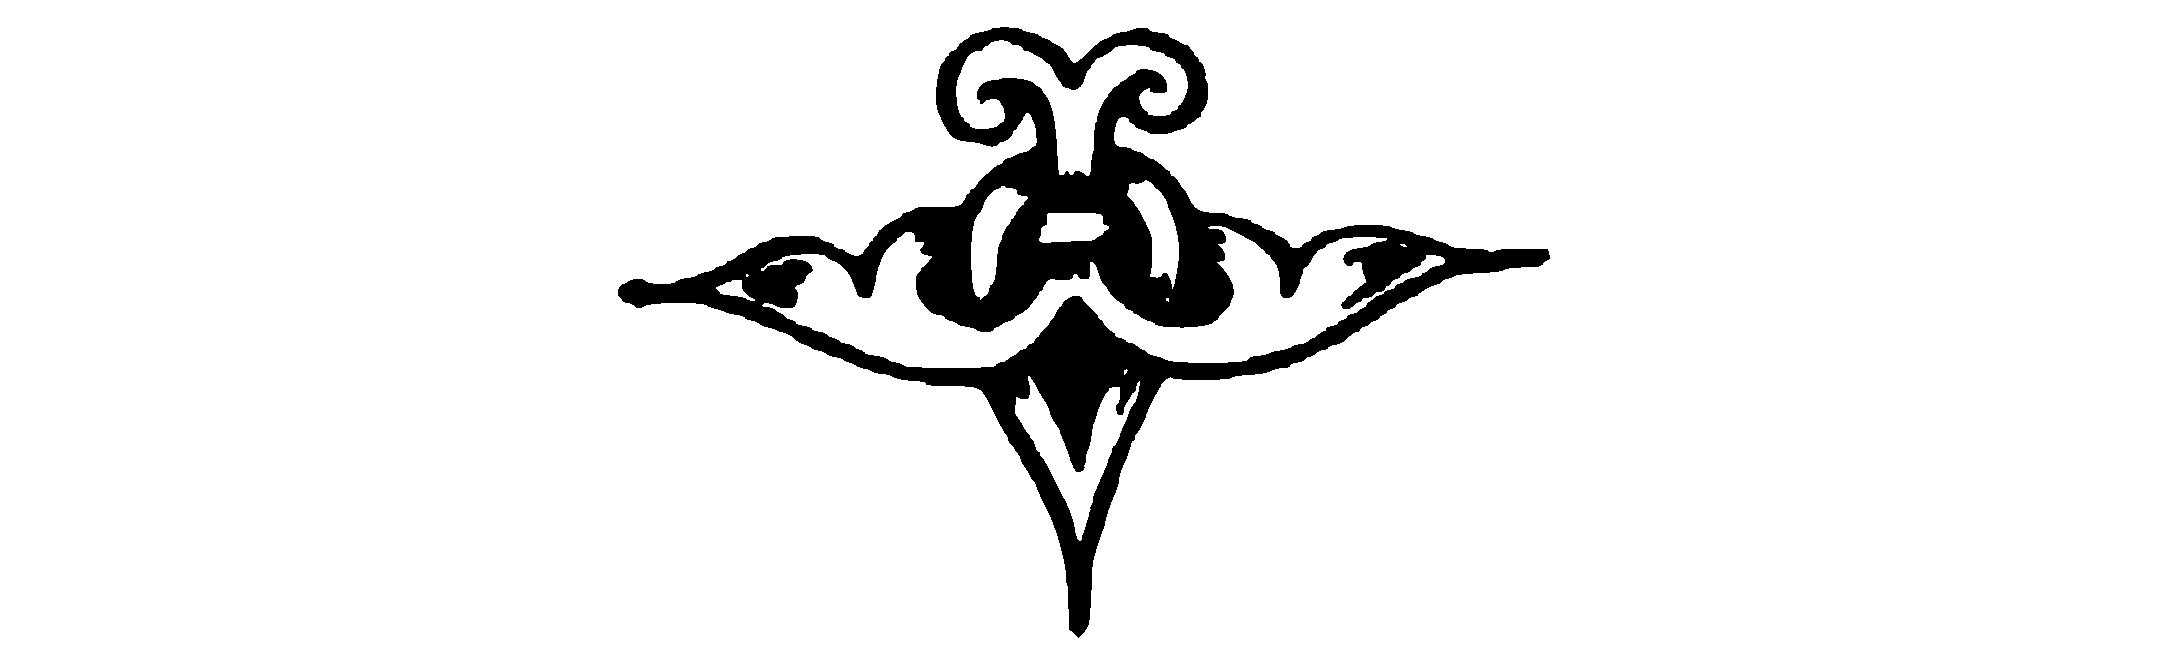
\includegraphics[width=0.20\textwidth]{uzor_end_2}\end{center}

\clearpage
\renewcommand{\ornament}{uzor_begin_2}
{\noparindent
\vspace*{-\headoff}
\includegraphics[width=\textwidth]{\ornament}}
\setlength\cftbeforepartskip{\savebeforepartskip}
\addtolength\cftbeforechapskip{-5pt}

% redefine empty pagestyle to include frame
\fancypagestyle{empty}{%
\fancyhf{} % clear all header and footer fields
\renewcommand{\headrulewidth}{0pt}
\renewcommand{\footrulewidth}{0pt}
\fancypageframe}

\vspace*{-5\baselineskip}
\tableofcontents\mychapterending

% set empty pagestyle back to defaults
\fancypagestyle{empty}{%
\fancyhf{} % clear all header and footer fields
\renewcommand{\headrulewidth}{0pt}
\renewcommand{\footrulewidth}{0pt}
}

\renewcommand{\ornament}{uzor_begin_10}





\mypart{О МОЛИТВЕ}\label{_o-molitve}
%http://www.molitvoslov.org/o-molitve



\mychapter{Как должно молиться в церкви}
%http://www.molitvoslov.org/text149.htm 

\begin{mymulticols}

\emph{ Православные христиане приняли от Святых Отец и исполняют во всем мире следующие обычаи:} 



1. Войдя в храм и осеняя себя крестным знамением, творят три малых поклона, произнося:

\begin{quote}{

«Создавый мя, Господи, помилуй». 

«Боже, милостив буди мне грешному». 

«Без числа согреших, Господи, прости мя».

}
\end{quote}


2. Затем, поклонившись направо и налево, стоят на месте и слушают псалмы и молитвы, читаемые в церкви, но не говорят про себя иных, собственных молитв, и не читают их по книжкам отдельно от церковного пения, ибо таких осуждает св. апостол Павел, как удаляющихся от церковного собрания (Евр. 10. 25). 



3. Поклоны малые и великие должно творить не по своему произволению, а по установлению св. апостолов и св. отец. Именно: при чтении Трисвятого («Святый Боже»), «Приидите, поклонимся» и троекратного «аллилуиа» трижды осенить себя крестным знамением, совершая малые поклоны; так же и при чтении «Сподоби, Господи», а равно и в начале великого славословия («Слава в вышних Богу») и после слов священника: «Слава Тебе, Христе Боже, упование наше». После каждого возгласа священника, а также при чтении чтецом «Честнейшую Херувим» осенять себя крестным знамением и творить малый поклон. 



Во дни будничные творить земные поклоны на литургии:

%\renewcommand{\theenumi}{\Asbuk{enumi}}

\begin{enumerate}

\item[а)] при начале пения «Достойно и праведно»; 

\item[б)] когда оканчивается молитва «Тебе поем»; 

\item[в)] в конце молитвы «Достойно есть» или Задостойника;

\item[г)] в начале молитвы «Отче наш»;

\item[д)] при изнесении св. Даров для причастия;

\item[е)] и при словах «Всегда, ныне и присно». 


\end{enumerate}


Hа утрени или всенощной, когда возглашается: «Богородицу и Матерь Света в песнех возвеличим». 



Во дни воскресные, а также от дня св. Пасхи до вечера дня св. Троицы, а равно от дня Рождества Христова по день Крещения, также в день Преображения и Воздвижения святые апостолы \emph{ воспретили} вовсе преклонять колена и творить \emph{ земные} поклоны, как о том свидетельствует св. Василий Великий в послании к блаженному Амфилохию. То же самое утвердили и Вселенские соборы I и VI; ибо воскресные и прочие Господские праздники содержат воспоминание о нашем примирении с Богом, по слову Апостола: «Уже неси раб, но сын» (Гал. 4, 7); cынам же не подобает рабское поклонение творити. 



4. Православным христианам не свойственно стоять на коленях, поднявши голову, но при словах священника: «Паки и паки, преклонше колена» и проч. повергаться ниц на землю; обычай же становиться на колени по собственному произволению, складывать руки и бить себя в грудь воспринят от западных еретиков, а в Православной Церкви недопускается. Православные христиане, согласно Уставу церковному, в \emph{ положенное} время творят земные поклоны, повергаясь ниц и снова становясь на ноги. 



5. Когда в церкви осеняют народ крестом или Евангелием, образом или Чашей, то все крестятся, преклоняя главу, а когда осеняют свечами или благословляют рукой, или кадят к предстоящим, то православным христианам не должно креститься, а только наклонить голову; лишь в Светлую седмицу Пасхи, когда кадит священник с Kрестом в руке, то все крестятся и говорят: «Воистину воскресе». Так должно различать поклонение пред святыней и пред людьми, хотя и в священном сане. 



6. Принимая благословение священника или епископа, христиане целуют его десницу, но не крестятся перед этим. Не должно целовать у духовных лиц левую руку, ибо сие свойственно только иудеям, но \emph{ правую}, через которую передается благословение. 



7. Крестное же знамение, по учению cвятых oтец, должно совершать так: сложив троеперстно правую руку, возлагать ее на лоб, на чрево, на правое плечо и на левое, и потом уже, положив на себя крест, наклоняться; o тех же, которые знаменуют себя всей пятерней или кланяются, не окончив еще креста, или машут рукой по воздуху или по груди своей, сказано в Златоусте: «Тому неистовому маханию беси радуются». Напротив, крестное знамение, совершаемое истово с верою и благоговением, устрашает бесов, утишает греховные страсти и привлекает Божественную благодать. 

\end{mymulticols}


\mychapterending

\mychapter{Правила о поклонах и крестном знамении}
%http://www.molitvoslov.org/text148.htm 

\begin{mymulticols}

\mysubtitle{Креститься \emph{ без поклонов:}}

\begin{enumerate}

\item В середине шестопсалмия на «аллилуиа» три раза. 

\item В начале «Верую». 

\item На отпусте «Христос, истинный Бог наш». 

\item В начале чтения Священного Писания: Евангелия, Апостола и паремий. 

\end{enumerate}

\mysubtitle{Креститься \emph{ с поясным поклоном:}}

\begin{enumerate}

\item При входе в храм и при выходе из него "--- три раза. 

\item При каждом прошении ектении после пения «Господи, помилуй», «Подай, Господи», «Тебе, Господи». 

\item При возгласе священнослужителя, воздающего славу Святой Троице. 

\item При возгласах «Приимите, ядите», «Пийте от нея вси», «Твоя от Твоих». 

\item При словах «Честнейшую Херувим». 

\item При каждом словe «поклонимся», «поклонение», «припадем». 

\item Во время слов «Аллилуиа», «Святый Боже» и «Приидите, поклонимся» и при возгласе «Слава Тебе, Христе Боже», перед отпустом "--- по три раза. 

\item На каноне на 1-й и 9-й песни при первом взывании к Господу, Божией Матери или святым.

\item После каждой стихиры (причем, крестится тот клирос, который оканчивает петь).

\item На литии после каждого из первых трех прошений ектении "--- по 3 поклона, после двух остальных "--- по одному.

\end{enumerate}

\mysubtitle{Креститься \emph{ с земным поклоном:}}

\begin{enumerate}
\item В пост при входе в храм и при выходе из него "--- 3 раза. 

\item В пост после каждого припева к песне Богородицы «Тя величаем». 

\item В начале пения «Достойно и праведно есть». 

\item После «Тебе поем». 

\item После «Достойно есть» или Задостойника. 

\item При возгласе: «И сподоби нас, Владыко». 

\item При выносе Святых Даров, при словах «Со страхом Божиим и верою приступите», и второй раз "--- при словах «Всегда, ныне и присно». 

\item В Великий пост, на Великом повечерии, при пении «Пресвятая Владычице» "--- на каждом стихе; при пении «Богородице Дево, радуйся» и проч. на великопостной вечерне совершаются три поклона. 

\item В пост, при молитве «Господи и Владыко живота моего». 

\itemВ пост при заключительном пении: «Помяни мя, Господи, егда приидеши во Царствии Твоем». Всего 3 земных поклона.

\end{enumerate}




\mysubtitle{Поясной поклон \emph{ без крестного знамения}}

\begin{enumerate}

\item При словах священника «Мир всем»

\item «Благословение Господне на вас»,

\item «Благодать Господа нашего Иисуса Христа», 

\item «И да будут милости Великаго Бога» и

\item При словах диакона «И во веки веков» (после возгласа священника «Яко свят еси, Боже наш» перед пением Трисвятого). 


\end{enumerate}





\mysubtitle{Креститься не положено}


\begin{enumerate}


\item Во время псалмов.

\item Вообще во время пения.

\item Во время ектений тому клиросу, который поет ектенийные припевы

\item Креститься и класть поклоны нужно по окончании пения, а никак не про последних словах.


\end{enumerate}






\mysubtitle{Не допускается земных поклонов:}






Во дни воскресные, в дни от Рождества Христова до Крещения, от Пасхи до Пятидесятницы, в праздник Преображения и Воздвижения (в сей день три земных поклона Кресту). Поклоны прекращаются от вечернего входа под праздник до «Сподоби, Господи» на вечерне в самый день праздника.

\end{mymulticols}

\mychapterending

\mychapter{Поучение святителя Игнатия Брянчанинова о молитвенном правиле}
%http://www.molitvoslov.org/text147.htm 

\begin{mymulticols}

Войдя в комнату твою, и, затворив дверь твою, помолись Отцу твоему, Который втайне; и Отец твой, видящий тайное, воздаст тебе явно… (Мф. 6, 6).

Господь, заповедавший уединенную молитву, очень часто Сам, во время Своего земного странствования, как повествует Евангелие, пребывал в ней. Он не имел где главу подклонить: и потому часто заменяли для него безмолвную, спокойную келлию безмолвные вершины гор и тенистые виноградники.

Темнота ночи закрывает предметы от любопытных взоров, тишина безмолвия не развлекает слуха. В безмолвии и ночью можно молиться внимательнее. Господь избирал для молитвы Своей преимущественное уединение и ночь, избирал их с тем, чтобы мы не только повиновались Его заповеди о молитве, но и следовали Его примеру. Для Самого Господа нужна ли была молитва? Пребывая, как человек, с нами на Земле, Он, как Бог, неразлучно был с Отцом и Духом, имел с Ними единую Божественную волю и Божественную власть.

«Войдя в комнату твою, и, затворив дверь твою, помолись Отцу твоему, Который втайне». Пусть о молитве твоей не знает никто: ни друг твой, ни родственник, ни само тщеславие, сожительствующее сердцу твоему и подстрекающее высказать кому-нибудь о молитвенном подвиге твоем, намекнуть о нем.

Затвори двери келлии твоей от людей приходящих для пустословия, для похищения у тебя молитвы; затвори двери ума от посторонних помышлений, которые предстанут, чтобы отвлечь тебя от молитвы; затвори двери сердца от ощущений греховных, которые будут покушаться смутить и осквернить тебя, и помолись.

Не дерзни приносить Богу многоглагольных и красноречивых молитв, тобой сочиненных, как бы они не казались тебе сильны и трогательны: они "--- произведение падшего разума и, будучи жертвой оскверненной, не могут быть приняты на духовный жертвенник Божий. А ты, любуясь изящными выражениями сочиненных тобою молитв и признавая утонченное действие тщеславия и сладострастия за утешение совести, и даже благодати, увлечешься далеко от молитвы; увлечешься далеко от молитвы в то самое время, когда тебе будет представляться, что ты молишься обильно и уже достиг некоторой степени богоугождения.

Душа, начинающая путь Божий, погружена в глубокое неведение всего Божественного и духовного, хотя бы она была и богата мудростию этого мира. По причине неведения она не знает, как и сколько надо ей молиться. Для вспомоществования младенчествующей душе Святая Церковь установила молитвенные правила.

Молитвенное правило есть собрание нескольких молитв, сочиненных Боговдохновенными святыми отцами, приспособленное к известному обстоятельству и времени.

Цель правила "--- доставить душе недостающее ей количество молитвенных мыслей и чувств, притом мыслей и чувств правильных, святых, истинно богоугодных. Такими мыслями и чувствами наполнены благодатные молитвы святых отцов.

Для молитвенного упражнения утром имеется особое собрание молитв, называемое утренними молитвами, или утренним правилом; для ночного моления пред отшествием ко сну "--- другое собрание молитв, именуемое молитвами на сон грядущим, или вечерним правилом. Особенное собрание молитв прочитывается готовящимися ко причащению Святых Христовых Таин и называется правилом ко Святому Причащению. Посвятившие большую часть своего времени благочестивым упражнениям (монахи) прочитывают около третьего часа пополудни особенное собрание молитв, называемое ежедневным, или иноческим правилом. Иные прочитывают ежедневно по нескольку кафизм, по нескольку глав из Нового Завета, полагают несколько поклонов "--- все это называется правилом.

Правило! Какое точное название, заимствованное из самого действия, производимого на человека молитвами, называемым правилом! Молитвенное правило направляет правильно и свято душу, научает ее поклоняться Богу Духом и Истиною (Ин. 4, 23), между тем как душа, будучи предоставлена самой себе, не могла бы идти правильно путем молитвы. По причине своего повреждения и омрачения грехом,она совращалась бы непрестанно в стороны, нередко в пропасти, то в рассеянность, то в мечтательность, то в различные пустые и обманчивые призраки высоких молитвенных состояний, сочиняемых ее тщеславием и сластолюбием.

Молитвенные правила удерживают молящегося в спасительном расположении смирения и покаяния, научая его непрестанному самоосуждению, питая его умилением, укрепляя надеждой на Всеблагого и Всемилосердого Бога, увеселяя миром Христовым, любовию к Богу и ближним.

Как возвышенны и глубоки молитвы ко Святому Причащению! Какое превосходное приготовление они доставляют приступающему к Святым Христовым Тайнам! Они убирают и украшают дом души чудными помышлениями и ощущениями, столь благоугодными Господу. Величественно изображено и объяснено в этих молитвах величайшее из Таинств христианских; в противоположность этой высоте живо и верно исчислены недостатки человека, показаны его немощь и недостоинство. Из них сияет, как солнце с неба, непостижимая благость Бога, по причине которой Он благоволит тесно соединяться с человеком, несмотря на ничтожность человека.

Утренние молитвы так и дышат бодростью, свежестью утра: увидевший свет чувственного солнца и свет земного дня научается желать зрения высшего, духовного Света и Дня бесконечного, производимых Солнцем Правды "--- Христом.

Краткое успокоение сном во время ночи "--- образ положительного сна во мраке могилы. И напоминают нам молитвы на сон грядущим о нашем переселении в вечность, обозревают всю нашу деятельность в течение дня, научают приносить Богу исповедание соделанных согрешений и покаяние в них.

Молитвенное чтение акафиста Сладчайшему Иисусу, кроме собственного своего достоинства, служит превосходным приготовлением к упражнению Молитвой Иисусовой, которая читается так: «Господи Иисусе Христе, Сыне Божий, помилуй мя, грешнаго». Эта молитва составляет почти единственно упражнение преуспевших подвижников, достигших (христианской) простоты и чистоты, для которых всякое многомышление и многословие служат обременительным развлечением. Акафист показывает, какими мыслями может быть сопровождаема Молитва Иисусова, представляющаяся для новоначальных крайне сухой. Он (акафист) изображает только прошение грешника о помиловании Господом Иисусом Христом, но этому прошению даны разноообразные формы, сообразно младенчественности ума новоначальных. Так младенцам дают пищу, предварительно размягченную.

В акафисте Божией Матери воспето воплощение Бога Слова и величие Божией Матери, Которую за рождение Ею вочеловечившегося Бога «ублажают все роды» (Лк. 1, 48). Как бы на большой картине бесчисленными дивными чертами, красками, оттенками изображено в акафисте великое Таинство вочеловечения Бога Слова. Удачным освещением оживляется всякая картина "--- и необыкновенным светом благодати озарен акафист Божией Матери. Свет этот действует сугубо: им просвещается ум, он него сердце исполняется радости и извещения. Непостижимое приемлется как вполне постигнутое, по чудному действию, производимому (словами акафиста) на ум и сердце.

Многие благоговейные христиане, особенно иноки, совершают очень продолжительное вечернее правило, пользуясь тишиной и мраком ночи. К молитвам на сон грядущим они присоединяют чтение кафизм, чтение Евангелия, Апостола, чтение акафистов и поклоны с Молитвой Иисусовой… рабы Христовы плачут в тишине своих келлий, изливая усердные молитвы пред Господом… В веселии и бодрости духа, в сознании и ощущении необыкновенной способности к богомыслию и ко всем благим делам встречают рабы Божии тот день, которому предшествующую ночь они провели в молитвенном подвиге.

Господь повергался на колени во время молитвы Своей "--- и ты не должен пренебрегать коленопреклонениями, если имеешь достаточно сил для совершения их. Поклонением до лица земли, по объяснению отцов, изображается наше падение, а восстанием с земли "--- наше искупление (Слова св. Феолипта. Добротолюбие, ч.2). Пред началом вечернего правила особенно полезно положить посильное число поклонов, чтобы приготовиться к усердному и внимательному чтению правила.

При совершении правила и поклонов никак нельзя спешить; надо совершать и правила, и поклоны с возможной неспешностью и вниманием. Лучше меньше прочитать молитв и меньше положить поклонов, но со вниманием, чем много и без внимания.

Избери себе правило, соответствующее силам. Сказанное Господом о субботе, что она для человека, а не человек для нее (Мк. 2, 27), можно и нужно отнести ко всем благочестивым подвигам, а также и к молитвенному правилу. Молитвенное правило "--- для человека, а не человек "--- для правила: оно должно способствовать к достижению человеком духовного преуспеяния, а не служить бременем неудобоносимым (тягостной обязанностью), сокрушающим телесные силы и смущающим душу. Тем более оно не должно служить поводом к гордостному и пагубному самомнению, к пагубному осуждению и унижению ближних.

Благоразумно избранное молитвенное правило, соответственно силам и роду жизни, является большим подспорьем для подвизающегося о своем спасении. Совершение его в положенные часы обращается в навык (от постоянства), в необходимую естественную потребность. Стяжавший этот блаженный навык, как только приближается к обычному месту совершения правила, так душа его уже исполняется молитвенным настроением: он не успел еще произнести ни одного слова из читаемых им молитв, а уже сердце наполняется умилением, и весь ум углубляется во внутренюю клеть (сердце).

«Предпочитаю,"--- сказал великий отец Матой,"--- непродолжительное правило, но постоянно исполняемое, продолжительному, но в скором времени оставляемому». А такую участь всегда имеют молитвенные правила, несоразмерные силам: при первом порыве горячности подвижник выполняет их, некоторое время, конечно, обращая больше внимания на количество, чем на качество, потом изнеможение, производимое подвигом, превосходящим силы, постепенно принуждает его сокращать и сокращать правило.

Часто подвижники, безрассудно установившие для себя обременительное правило, переходят от многотрудного правила к оставлению всякого правила. По оставлении правила, и даже при одном сокращении его, непремено нападает на подвижника смущение. От смущения он начинает чувствовать душевное расстройство. От расстройства рождается уныние. Усилившись, оно производит расслабление и исступление, а от действия их безрассудный подвижник предается праздной, рассеянной жизни, с равнодушием впадает в самые тяжкие согрешения.

Избрав для себя соразмерное силам и душевной потребности молитвенное правило, старайся тщательно и постоянно исполнять его: это нужно для поддержания нравственных сил души твоей, как нужно для поддержания телесных сил ежедневное, в известые часы, достаточное употребление здоровой пищи.

«Не за оставление псалмов осудит нас Бог в день Суда Своего,"--- говорит святой Исаак Сирин,"--- не за оставление молитвы, но за последующий оставлению их вход в нас бесов. Бесы, когда найдут место, войдут и затворят двери очей наших, тогда исполняют нами, их орудиями, насильственно и нечисто, с лютейшим отмщением, все воспрещенное Богом. И по причине оставления малого (правила), за которое (мы) сподобляемся заступления Христова, мы делаемся подвластными (бесам), как написано некоторым премудрым отцом: ,,Непокоряющий воли своей Богу, подчинится сопернику своему``. Эти (правила), кажущиеся тебе малыми, соделаются для тебя стенами против старающихся пленить нас. Совершение этих (правил) внутри келлии премудро установлено учредителями Церковного Устава, по откровению свыше, для хранения жития нашего» (Исаак Сирин, Слово 71).

Великие отцы, пребывавшие от обильного действия благодати Божией в непрестанной молитве, не оставляли и правил своих, которые навыкли они совершать в известные часы нощеденствия (ночных и дневных молитв). Многие доказательства этого видим в их житиях: преподобный Антоний Великий, совершая правило девятого часа "--- церковный девятый час соответствует третьему часу пополудни,"--- сподобился Божественного откровения; когда Преподобный Сергий Радонежский занимался молитвенным чтением акафиста Божией Матери, явилась ему Пресвятая Дева в сопровождении апостолов Петра и Иоанна.

Возлюбленные! Покорим свою свободу правилу: оно, лишив нас свободы пагубной, свяжет нас только для того, чтоб доставить нам свободу духовную, свободу во Христе. Цепи сначала покажутся тягостными, потом сделаются драгоценными для связанного ими. Все святые Божии приняли на себя и несли благое иго молитвенного правила; подражанием им и мы последуем в этом случае Господу нашему Иисусу Христу, Который вочеловечившись и указав нам Собой образ поведения, действовал так, как действовал Отец Его (Ин. 5, 19), говорил то, что заповедал Ему Отец (Ин. 12, 49), имел целью исполнить во всем волю Отца (Ин. 5, 30). Воля Отца и Сына и Святаго Духа "--- одна. По отношению к людям она заключается в спасении людей.

Всесвятая Троице, Боже наш! Слава Тебе! Аминь.

\bigskip

{\itshape (Епископ Игнатий Брянчанинов. Сочинения. Аскетические опыты.
СПб., 1865 т.2, с. 181--191. Публикуется в сокращении.)}

\end{mymulticols} 


\mychapterending

\mychapter{Чин келейного чтения канонов и акафистов}
%http://www.molitvoslov.org/text894.htm 


\begin{mymulticols}



\myemph{Перед началом всякого правила и по окончании его кладутся следующие поклоны (земные или поясные), кои называются седмипоклонный начал.}




Боже, милостив буди мне грешному. \myemph{(Поклон)} 

Боже, очисти мя грешнаго и помилуй мя. \myemph{(Поклон)}




Создавый мя, Господи, помилуй мя. \myemph{(Поклон)}




Без числа согреших, Господи,прости мя. \myemph{(Поклон)}




Владычица моя, Пресвятая Богородице, спаси мя грешнаго. \myemph{(Поклон)}




Ангеле, хранителю мой, от всякого зла сохрани мя. \myemph{(Поклон)}




Святой апостоле (\myemph{или} мучениче, \myemph{или} преподобный отче), \myemph{имя}) моли Бога о мне. \myemph{(Поклон)}







\mysubtitle{Также:} \MolitvamiSviatyhOtecNashih

Слава Тебе, Боже наш, слава Тебе.

\TsariuNebesnyj

\TrisviatoePoOtcheNash

\mysubtitle{Псалом 50-й:}

\PsalmFifty

\mysubtitle{Символ веры}

\SymbolOfFaith

\myemph{И чти каноны c акафисты.}


\myemph{Посем:} \Chestneyshuyu \myemph{(Поклон)}

\TrisviatoePoOtcheNash

\mysubtitle{Тропари:}

\TroparPomilujNas

\myemph{И молитвы на сон грядущим.} 

\myemph{Готовящимся ко св. Причащению нужно обязательно вечером прочитать три канона: Спасителю, Божией Матери и Ангелу-хранителю, и акафист Спасителю и Божией Матери. Желающие же ежедневно выполнять это вечернее правило и получают от этого великую духовную пользу.}

\end{mymulticols}

\mychapterending

\mychapterz{О молитве Иисусовой}{\vspace{-0.5\baselineskip}О молитве Иисусовой}
%http://www.molitvoslov.org/text146.htm 

\vspace{-\baselineskip}

\begin{mymulticols}

\myemph{Иисусова молитва творится с благословения и под контролем духовника.}

У апостола Павла в первом послании к Солунянам (5, 16) сказано: «непрестанно молитесь». Как же это непрестанно молиться? "--- Часто творить молитву Иисусову: «Господи Иисусе Христе, Сыне Божий, помилуй мя». Если кто навыкнет этому призыванию, тот будет ощущать великое утешение и потребность всегда творить эту молитву и она как бы сама собой в нем будет твориться. 

Хотя вначале враг рода человеческого будет мешать в этом, наводить большую тяготу, лень, скуку, одолевающий сон, но, преодолевши все это, с помощью Божией, получишь покой душе твоей, духовную радость, расположение к людям, умиротворение помыслов, благодарение Богу. 

В самом имени Иисуса Христа заключается великая благодатная сила. 

Многие святые и праведные люди советуют как можно чаще, почти непрерывно, творить молитву Иисусову. 

Св. Иоанн Златоуст говорит: «Должно всякому, если он, пьет ли, сидит ли, служит ли, путешествует ли, или другое что делает, непрестанно вопить: ,,Господи, Иисусе Христе, Сыне Божий, помилуй мя``, да имя Господа Иисуса Христа, сходя в глубину сердечную, смирит змия пагубного, душу же спасет и оживотворит». 

Преподобный Серафим Саровский: «,,Господи Иисусе Христе, Сыне Божий, помилуй мя грешного``: в этом да будет все твое внимание и обучение. Ходя, сидя, делая и в церкви до богослужения стоя, входя и выходя, сие непрестанно держи в устах и в сердце твоем. С призыванием имени Божия таким образом ты найдешь покой, достигнешь чистоты духовной и телесной и вселится в тебя Святый Дух, Источник всех благ, и управит он тебя в святыне, во всяком благочестии и чистоте». 

Епископ Феофан Затворник: «Чтобы удобнее навыкнуть памятованию о Боге, для этого для христиан ревностных есть особый прием, именно "--- непрестанно повторять коротенькую "--- слова в два-три "--- молитовку. Большей частью это есть: ,,Господи, помилуй! "--- Господи, Иисусе Христе, помилуй мя грешнаго (или грешную)``. Если вы этого еще не сделали, так вот слышьте, и если так не делали, так начинайте делать с этих пор». 

«Истинно решивший служить Господу Богу должен упражняться в памяти Божией и непрестанной молитве Иисусу Христу, говоря умом: ,,Господи, Иисусе Христе, Сыне Божий, помилуй мя грешнаго``. Таковым упражнением, при охранении себя от рассеяния и при соблюдении мира совести, можно приблизиться к Богу и соединиться с Ним. Ибо, по словам св. Исаака Сирина, без непрестанной молитвы мы приблизиться к Богу не можем» (Преп. Серафим Саровский). 

О. Иоанн Кронштадский также часто советовал творить молитву Иисусову.

\end{mymulticols}

\mychapterending

\mychapter{О даровании молитвы}
%http://www.molitvoslov.org/text145.htm 






Научи мя, Господи, усердно молиться Тебе со вниманием и любовию, без которых молитва не бывает услышана! Да не будет у меня небрежной молитвы во грех мне!




\mychapterending

\mychapter{Молитва человека, страдающего рассеянием, невниманием, нерадением в молитве}
%http://www.molitvoslov.org/text144.htm 






Рассеянный ум мой собери, Господи, и оледеневшее сердце очисти, яко Петру даяй мне покаяние, яко мытарю "--- воздыхание, и яко блуднице "--- слезы, да велиим гласом зову Ти, Боже, спаси мя, яко Един Благоутробен и Человеколюбец. 




\mychapterending

\mychapter{Молитва Оптинских старцев о даровании молитвы Иисусовой}
%http://www.molitvoslov.org/text137.htm 

\begin{mymulticols}

Господи Иисусе Христе, Сыне Божий! Имени Твоему покланяются ангели и человецы, Твоего имени трепещут адские силы, Твое имя верное оружие на прогнание супостата, Твое имя попаляет грехи и страсти, Твое имя подает силу в подвигах, собирает воедино рассеянный ум и, во исполнении заповедей Твоих, обогащает добродетелями, Твое имя творит чудеса и соединяет нас с Тобою, дарует мир и радость о Духе Святом, а в жизни будущей "--- Царство Небесное. Сего ради я, недостойный раб Твой, молюся Тебе: прожени от нас неведение духовное, просвети познанием Божественной истины и научи нас незаблудно, во смирении, внимательно, с чувством покаяннаго сокрушения, устами, умом и сердцем творить непрестанно молитву сию: \textbf{«Господи Иисусе Христе, Сыне Божий, помилуй мя, грешнаго»}. Ты бо рекл еси, Господи, пречистыми устами Твоими: «Аще что просите во имя Мое, Аз сотворю». Се, молитвами Пречистыя Матери Твоея, святителя Иоасафа Белградскаго, святителя Николая Мирликийскаго, преподобнаго Серафима Саровскаго и всех преподобных отец наших о даровании прошу молитвы Иисусовой, молитвы Пресвятаго и Всемогущаго Имени Твоего. Услыши мя, обещавый услышать всех призывающих Тя во истине. Твое бо есть еже миловати и спасати, и даровати просимое молящемуся во славу Твою со Отцем и Святым Духом. Аминь. 


\end{mymulticols}



{\centering\myemph{(Если молитва прочитана невнимательно, прочитать еще раз.)}\par}


\mychapterending

\mychapter{Правило преподобного Серафима Саровского для мирян}
%http://www.molitvoslov.org/text132.htm 

\begin{mymulticols}

Молитву преподобный Серафим Саровский считал для жизни столь же необходимой, как воздух. Он просил и требовал от своих духовных детей, чтобы они непрестанно молились, и заповедал им молитвенное правило, оставшееся под именем «Правила отца Серафима». 

Пробудившись от сна и ставши на избранном месте, всякий должен оградить себя крестным знамением и, став на избранном месте, читать ту спасительную молитву, которую людям передал Сам Господь, то есть «Отче наш» (трижды), потом «Богородице Дево, радуйся» (трижды), и, наконец, единожды Символ веры. Совершив это утреннее правило, всякий христианин пусть отходит на свое дело и, занимаясь дома или находясь в пути, должен читать тихо про себя: «Господи Иисусе Христе, Сыне Божий, помилуй мя грешнаго». Если же окружают люди, то, занимаясь делом, говорить только умом: «Господи, помилуй», и так продолжать до самого обеда. Перед обедом совершить утреннее правило. 

После обеда, исполняя свое дело, всякий должен читать тихо: «Пресвятая Богородице, спаси мя грешнаго», что продолжать до самой ночи. 

Когда же случится проводить время в уединении, нужно читать: «Господи Иисусе Христе, Богородицею помилуй мя грешнаго», а ложась спать на ночь, всякий христианин должен повторить утреннее правило, и после него с крестным знамением засыпать. При этом св. старец говорил, указывая на опыт св. отeц, что, если христианин будет держаться этого малого правила, как спасительного якоря среди волн мирской суеты, со смирением исполняя его, то может достигнуть высокой меры духовной, ибо эти молитвы суть основание христианства: первая "--- как слово Самого Господа и поставленная Им в образец всех молитв, вторая принесена с неба Архангелом как приветствие Пресвятой Деве, Матери Господа. Последняя же заключает все догматы веры. 

Имеющий время пусть читает Евангелие, Апостол, другие молитвы, акафисты, каноны. Если же кому-то невозможно выполнять и это правило "--- слуге, подневольному человеку "--- то мудрый старец советовал выполнять это правило и лежа, и при ходьбе, и при деле, помня слова Писания: «Всяк, иже призовет имя Господне, спасется». 

\end{mymulticols}


\mychapterending

\mychapter{О молитве. Св.Иоанн Златоуст}
%http://www.molitvoslov.org/text152.htm 

\begin{mymulticols}

Молитва имеет два вида: первый "--- славословие со смиренномудрием, а второй, низший "--- прошение. Посему, молясь, не вдруг приступай к прошению… Начиная молитву, оставь себя самого, жену, детей, расстанься с землей, минуй небо, оставь всякую тварь видимую и невидимую, и начни славословием все Сотворившего; и когда будешь славословить, не блуждай умом туда и сюда, не баснословь по-язычески, но выбирай слова из Святых Писаний… Когда же кончишь славословие… тогда начни со смиренномудрием и говори: недостоин я, Господи, говорить пред Тобою, потому что я весьма грешен,"--- более всех грешников грешен я. Так молись со страхом и смиренномудрием. Когда же совершишь обе эти части славословия и смиренномудрия, тогда проси уже, чего ты должен просить, то есть не богатства, не славы земной, не здравия телесного, потому что Он Сам знает, что полезно каждому; но, как поверено тебе, проси Царствия Божия.


\bigskip\emph{Свт. Иоанн Златоуст}

\end{mymulticols}



\mychapterending

\mychapter{О Храмовой молитве}
%http://www.molitvoslov.org/text151.htm 

\begin{mymulticols}

В общих церковных богослужениях не исключается, конечно, частная молитва, но главное внимание молящихся все же должно быть сосредоточено на совершающемся богослужении. Молитва в храме "--- молитва соборная; в ней участвуют и клирики, и миряне, т.~е. вся земная Церковь. Поэтому и сила молитвеннаго духа в такой молитве сильнее, чем в частной домашней молитве. В наших храмовых богослужениях каждый найдет моления о том, что ему именно нужно, а кроме того, приносятся еще моления о всех ближних, о властях предержащих, о всей Церкви, благодарения, славословия Господу за Его милости, как учит ап.Павел: «Итак прежде всего прошу совершать молитвы, прошения, моления, благодарения за всех человеков, за царей и за всех начальствующих, дабы проводит нам жизнь тихую и безмятежную во всяком благочестии и чистоте» (Тим.II, 1--2). Все это есть в нашем богослужении, требуется лишь внимание ума и сердца со стороны молящихся и толковое чтение и пение со стороны клира. Разумное и сердечное участие в храмовом богослужении "--- самая действенная, самая живая жизнь в Церкви "--- этом таинственном Теле Христовом (I Кор. 12,27). В самом деле: вот мы все "--- клирики и миряне "--- составляющие Церковь видимую, земную; вот "--- видимые образы невидимо присутствующей Церкви прославленной, невидимой, во главе с Царицей неба и земли "--- Пречистой Богоматерью; все сонмы ангелов и святых. А на св. Престоле в алтаре воистину "--- в Своей Плоти и Крови "--- восседает Сам Глава всей Церкви, Пастыреначальник Господь Иисус Христос.

Перед лицем такого высочайшаго собора "--- с каким благоговением и трепетом должны стоять мы! С каким вниманием и страхом должны клирики совершать свое служение! И как-то странно в этом таинственном и связанном собрании Церкви видимой и невидимой взывать ко Господу со своими личными нуждами. Только очень уже большая, невыносимая тогу может заставить сделать это. А то хочется забыть себя, свою суетную жизнь и безраздельно слиться в священном трепете с ликованием невидимых, но чувствуемых каждой верующей душой, сонмов святых и ангелов, «Всякое ныне житейское отложим попечение» "--- взывает к нам на литургии невидимый сонм херувимов, предстоящих огненному Престолу Господа славы, Господа силы!..

Да и нужно отложить все! Нужно все силы ума и сердца направить на то, чтобы войти в жизнь, в ликование Церкви. А для этого нужно ясно сознавать смысл и цель каждаго движения. Маловеры упрекают Православие в том, что оно все ушло в обрядность. Но если сердцем и умом уметь следить за ходом богослужения, связывая тексты с действиями, тот открывается такая дивная, несказуемая жизнь, которую можно только переживать, но о которой нельзя говорить; это частица того, о чем ап. Павел писал: «Но вы приступили к горе Сиону и ко граду Бога живаго, к небесному Иерусалиму и тьмам Ангелов. К торжествующему собору и Церкви первенцев, написанных на небесах, и к Судии всех Богу, и к духам праведников, достигших совершества, и к ходатаю новаго завета Иисуса» (Евр.XII, 22--24), и еще: не видел того глаз, не слышало того ухо, и не приходило то на сердце человеку, что приготовил Бог любящим Его» (1 Кор. 11, 9). Поэтому справедливо утверждение, что храм "--- рай на земле.

\bigskip

{\itshape Сер.Л. "--- Лит. оч. "--- № 35, 1930

«Приходская жизнь», декабрь 1980}

\end{mymulticols}


\mychapterending

%/content/soderzhanie



\bfseries Смотреть весь раздел &rarr;\normalfont{} 



\mypart{МОЛИТВЫ}\label{_content_molitvi}
%http://www.molitvoslov.org/content/molitvi

\mychapter{Молитва Господня. Отче наш}\begin{mymulticols}

%http://www.molitvoslov.org/node/37

\myfigure{Spasnatrone}

Отче наш, Иже еси на небесех! Да святится имя Твое, да приидет Царствие Твое, да будет воля Твоя, яко на небеси и на земли. Хлеб наш насущный даждь нам днесь; и остави нам долги наша, якоже и мы оставляем должником нашим; и не введи нас во искушение, но избави нас от лукаваго.

Отче наш, сущий на небесах! да святится имя Твое; да приидет Царствие Твое; да будет воля Твоя и на земле, как на небе; хлеб наш насущный дай нам на сей день; и прости нам долги наши, как и мы прощаем должникам нашим; и не введи нас в искушение, но избавь нас от лукавого. Ибо Твое есть Царство и сила и слава во веки. Аминь. (Матф. 6:9--13)


\end{mymulticols}

\mychapterending


\mychapter{Иисусова молитва}
%http://www.molitvoslov.org/text596.htm

\myfigure[0.5]{456}

{\centering Господи Иисусе Христе, Сыне Божий, помилуй мя, грешнаго.\par}

\mychapterending


\mychapter{Благодарение за всякое благодеяние Божие}\begin{mymulticols}
%http://www.molitvoslov.org/text889.htm

\myfigure{777}

\mysubtitle{Тропарь, глас 4-й}

Благодарни суще недостойнии раби Твои, Господи, о Твоих великих благодеяниих на нас бывших, славяще Тя хвалим, благословим, благодарим, поем и величаем Твое благоутробие, и рабски любовию вопием Ти: Благодетелю Спасе наш, слава Тебе.

\mysubtitle{Кондак, глас 3-й}

Твоих благодеяний и даров туне, яко раби непотребнии, сподобльшеся, Владыко, к Тебе усердно притекающе, благодарение по силе приносим, и Тебе яко Благодетеля и Творца славяще, вопием: слава Тебе, Боже Всещедрый.

\slavainynen

\Bogorodichen{Богородице, христианом Помощнице, Твое предстательство стяжавше раби Твои, благодарно Тебе вопием: радуйся, Пречистая Богородице Дево, и от всех нас бед Твоими молитвами всегда избави, Едина вскоре предстательствующая.}

\end{mymulticols}

\mychapterending


\mychapter{Молитвы утренние}\begin{mymulticols}
%http://www.molitvoslov.org/text893.htm

\myfigure{795}

\footnote{Напечатанное \emph{курсивом} (\myemph{пояснения} и \textbf{названия молитв}) не читается во время молитвы.}\myemph{  Востав от сна, прежде всякого другого дела, стань благоговейно, представляя себя пред Всевидящим Богом, и, совершая крестное знамение, произнеси:}

Во имя Отца, и Сына, и Святаго Духа, Аминь.

\medskip\myemph{ Затем немного подожди, пока все чувства твои не придут в тишину и мысли твои не оставят все земное, и тогда произноси следующие молитвы, без поспешности и со вниманием сердечным:}

\mysubtitle{Молитва мытаря \myemph{(Евангелие от Луки, глава 18, стих 13)}}

Боже, милостив буди мне грешному. \myemph{ (Поклон)}

\mysubtitle{Молитва предначинательная}

Господи Иисусе Христе, Сыне Божий, молитв ради Пречистыя Твоея Матере и всех святых, помилуй нас. Аминь.

Слава Тебе, Боже наш, слава Тебе.

\mysubtitle{Молитва Святому Духу}

Царю Небесный, Утешителю, Душе истины, Иже везде сый и вся исполняяй, Сокровище благих и жизни Подателю, прииди и вселися в ны, и очисти ны от всякия скверны, и спаси, Блаже, души наша\footnote{От Пасхи до Вознесения вместо этой молитвы читается тропарь: «Христос воскресе из мертвых, смертию смерть поправ, и сущим во гробех живот даровав». \myemph{(Трижды)} От Вознесения до Троицы начинаем молитвы со «Святый Боже…», опуская все предшествующие.

Это замечание относится и к молитвам на сон грядущим.
}.

\mysubtitle{Трисвятое}

Святый Боже, Святый Крепкий, Святый Безсмертный, помилуй нас. \myemph{ (Читается трижды, с крестным знамением и поясным поклоном.) }

Слава Отцу и Сыну и Святому Духу, и ныне и присно и во веки веков. Аминь.

\mysubtitle{Молитва ко Пресвятой Троице}

Пресвятая Троице, помилуй нас; Господи, очисти грехи наша; Владыко, прости беззакония наша; Святый, посети и исцели немощи наша, имене Твоего ради.

Господи, помилуй. \myemph{ (Трижды)}.

Слава Отцу и Сыну и Святому Духу, и ныне и присно и во веки веков. Аминь\footnote{Когда написано «Слава», «И ныне», надо читать полностью: «Слава Отцу и Сыну и Святому Духу», «И ныне и присно и во веки веков. Аминь»}.

\mysubtitle{Молитва Господня}

Отче наш, Иже еси на небесех! Да святится имя Твое, да приидет Царствие Твое, да будет воля Твоя, яко на небеси и на земли. Хлеб наш насущный даждь нам днесь; и остави нам долги наша, якоже и мы оставляем должником нашим; и не введи нас во искушение, но избави нас от лукаваго.

\mysubtitle{Тропари Троичные}

Воставше от сна, припадаем Ти, Блаже, и ангельскую песнь вопием Ти, Сильне: Свят, Свят, Свят еси, Боже, Богородицею помилуй нас.

\slavan

 От одра и сна воздвигл мя еси, Господи, ум мой просвети и сердце, и устне мои отверзи, во еже пети Тя, Святая Троице: Свят, Свят, Свят еси, Боже, Богородицею помилуй нас.

\inynen

 Внезапно Судия приидет, и коегождо деяния обнажатся, но страхом зовем\footnote{В церковнославянском языке нет звука ё, а поэтому надо читать «зовем», а не «зовём», «твое», а не «твоё», «мое», а не «моё» и т.~д.} в полунощи: Свят, Свят, Свят еси, Боже, Богородицею помилуй нас.

Господи, помилуй. \myemph{ (12 раз)}

\mysubtitle{Молитва ко Пресвятой Троице}

От сна востав, благодарю Тя, Святая Троице, яко многия ради Твоея благости и долготерпения не прогневался еси на мя, лениваго и грешнаго, ниже погубил мя еси со беззаконьми моими; но человеколюбствовал еси обычно и в нечаянии лежащаго воздвигл мя еси, во еже утреневати и славословити державу Твою. И ныне просвети мои очи мысленныя, отверзи моя уста поучатися словесем Твоим, и разумети заповеди Твоя, и творити волю Твою, и пети Тя во исповедании сердечнем, и воспевати всесвятое имя Твое, Отца и Сына и Святаго Духа, ныне и присно и во веки веков. Аминь.

Приидите, поклонимся Цареви нашему Богу. \myemph{ (Поклон)}

Приидите, поклонимся и припадем Христу, Цареви нашему Богу. \myemph{ (Поклон)}

Приидите, поклонимся и припадем Самому Христу, Цареви и Богу нашему. \myemph{ (Поклон)}

\mysubtitle{Псалом 50}

\PsalmFifty

\mysubtitle{Символ веры}

\SymbolOfFaith
  
\mysubtitle{Молитва первая, святого Макария Великого}

Боже, очисти мя грешнаго, яко николиже сотворих благое пред Тобою; но избави мя от лукаваго, и да будет во мне воля Твоя, да неосужденно отверзу уста моя недостойная и восхвалю имя Твое святое, Отца и Сына и Святаго Духа, ныне и присно и во веки веков Аминь.

\mysubtitle{ Молитва вторая, того же святого}

От сна востав, полунощную песнь приношу Ти, Спасе, и припадая вопию Ти: не даждь ми уснути во греховней смерти, но ущедри мя, распныйся волею, и лежащаго мя в лености ускорив возстави, и спаси мя в предстоянии и молитве, и по сне нощнем возсияй ми день безгрешен, Христе Боже, и спаси мя.

\mysubtitle{Молитва третья, того же святого}

К Тебе, Владыко Человеколюбче, от сна востав прибегаю, и на дела Твоя подвизаюся милосердием Твоим, и молюся Тебе: помози ми на всякое время, во всякой вещи, и избави мя от всякия мирския злыя вещи и диавольскаго поспешения, и спаси мя, и введи в Царство Твое вечное. Ты бо еси мой Сотворитель и всякому благу Промысленник и Податель, о Тебе же все упование мое, и Тебе славу возсылаю, ныне и присно и во веки веков. Аминь.

\mysubtitle{Молитва четвертая, того же святого}

Господи, Иже многою Твоею благостию и великими щедротами Твоими дал еси мне, рабу Твоему, мимошедшее время нощи сея без напасти прейти от всякаго зла противна; Ты Сам, Владыко, всяческих Творче, сподоби мя истинным Твоим светом и просвещенным сердцем творити волю Твою, ныне и присно и во веки веков. Аминь.

\mysubtitle{Молитва пятая, святого Василия Великого}

Господи Вседержителю, Боже сил и всякия плоти, в вышних живый и на смиренныя призираяй, сердца же и утробы испытуяй и сокровенная человеков яве предведый, Безначальный и Присносущный Свете, у Него же несть пременение, или преложения осенение; Сам, Безсмертный Царю, приими моления наша, яже в настоящее время, на множество Твоих щедрот дерзающе, от скверных к Тебе устен творим, и остави нам прегрешения наша, яже делом, и словом, и мыслию, ведением, или неведением согрешенная нами; и очисти ны от всякия скверны плоти и духа. И даруй нам бодренным сердцем и трезвенною мыслию всю настоящаго жития нощь прейти, ожидающим пришествия светлаго и явленнаго дне Единороднаго Твоего Сына, Господа и Бога и Спаса нашего Иисуса Христа, в оньже со славою Судия всех приидет, комуждо отдати по делом его; да не падше и обленившеся, но бодрствующе и воздвижени в делание обрящемся готови, в радость и Божественный чертог славы Его совнидем, идеже празднующих глас непрестанный, и неизреченная сладость зрящих Твоего лица доброту неизреченную. Ты бо еси истинный Свет, просвещаяй и освящаяй всяческая, и Тя поет вся тварь во веки веков. Аминь.

\mysubtitle{Молитва шестая, того же святого}

Тя благословим, вышний Боже и Господи милости, творящаго присно с нами великая же и неизследованная, славная же и ужасная, ихже несть числа, подавшаго нам сон во упокоение немощи нашея, и ослабление трудов многотрудныя плоти. Благодарим Тя, якo не погубил еси нас со беззаконьми нашими, но человеколюбствовал еси обычно, и в нечаянии лежащия ны воздвигл еси, во еже славословити державу Твою. Темже молим безмерную Твою благость, просвети наша мысли, очеса, и ум наш от тяжкаго сна лености возстави: отверзи наша уста, и исполни я Твоего хваления, яко да возможем непоколеблемо пети же и исповедатися Тебе, во всех, и от всех славимому Богу, Безначальному Отцу, со Единородным Твоим Сыном, и Всесвятым и Благим и Животворящим Твоим Духом, ныне и присно и во веки веков. Аминь.

\mysubtitle{Молитва седьмая, ко Пресвятой Богородице}

Воспеваю благодать Твою, Владычице, молю Тя, ум мой облагодати. Ступати право мя настави, путем Христовых заповедей. Бдети к песни укрепи, уныния сон отгоняющи. Связана пленицами грехопадений, мольбами Твоими разреши, Богоневесто. В нощи мя и во дни сохраняй, борющих враг избавляющи мя. Жизнодателя Бога рождшая, умерщвлена мя страстьми оживи. Яже Свет невечерний рождшая, душу мою ослепшую просвети. О дивная Владычня палато, дом Духа Божественна мене сотвори. Врача рождшая, уврачуй души моея многолетныя страсти. Волнующася житейскою бурею, ко стези мя покаяния направи. Избави мя огня вечнующаго, и червия же злаго, и тартара. Да мя не явиши бесом радование, иже многим грехом повинника. Нова сотвори мя, обетшавшаго нечувственными, Пренепорочная, согрешении. Странна муки всякия покажи мя, и всех Владыку умоли. Небесная ми улучити веселия, со всеми святыми, сподоби. Пресвятая Дево, услыши глас непотребнаго раба Твоего. Струю давай мне слезам, Пречистая, души моея скверну очищающи. Стенания от сердца приношу Ти непрестанно, усердствуй, Владычице. Молебную службу мою приими, и Богу благоутробному принеси. Превышшая Ангел, мирскаго мя превышша слития сотвори. Светоносная Сене небесная, духовную благодать во мне направи. Руце воздею и устне к похвалению, осквернены скверною, Всенепорочная. Душетленных мя пакостей избави, Христа прилежно умоляющи; Емуже честь и поклонение подобает, ныне и присно и во веки веков. Аминь.

\mysubtitle{Молитва восьмая, ко Господу нашему Иисусу Христу}

Многомилостиве и Всемилостиве Боже мой, Господи Иисусе Христе, многия ради любве сшел и воплотился еси, яко да спасеши всех. И паки, Спасе, спаси мя по благодати, молю Тя; аще бо от дел спасеши мя, несть се благодать, и дар, но долг паче. Ей, многий в щедротах и неизреченный в милости! Веруяй бо в Мя, рекл еси, о Христе мой, жив будет и не узрит смерти во веки. Аще убо вера, яже в Тя, спасает отчаянныя, се верую, спаси мя, яко Бог мой еси Ты и Создатель. Вера же вместо дел да вменится мне, Боже мой, не обрящеши бо дел отнюд оправдающих мя. Но та вера моя да довлеет вместо всех, та да отвещает, та да оправдит мя, та да покажет мя причастника славы Твоея вечныя. Да не убо похитит мя сатана, и похвалится, Слове, еже отторгнути мя от Твоей руки и ограды; но или хощу, спаси мя, или не хощу, Христе Спасе мой, предвари скоро, скоро погибох: Ты бо еси Бог мой от чрева матере моея. Сподоби мя, Господи, ныне возлюбити Тя, якоже возлюбих иногда той самый грех; и паки поработати Тебе без лености тощно, якоже поработах прежде сатане льстивому. Наипаче же поработаю Тебе, Господу и Богу моему Иисусу Христу, во вся дни живота моего, ныне и присно и во веки веков. Аминь.

\mysubtitle{Молитва девятая, к Ангелу хранителю}

Святый Ангеле, предстояй окаянной моей души и страстной моей жизни, не остави мене грешнаго, ниже отступи от мене за невоздержание мое. Не даждь места лукавому демону обладати мною, насильством смертнаго сего телесе; укрепи бедствующую и худую мою руку и настави мя на путь спасения. Ей, святый Ангеле Божий, хранителю и покровителю окаянныя моея души и тела, вся мне прости, еликими тя оскорбих во вся дни живота моего, и аще что согреших в прешедшую нощь сию, покрый мя в настоящий день, и сохрани мя от всякаго искушения противнаго, да ни в коем гресе прогневаю Бога, и молися за мя ко Господу, да утвердит мя в страсе Своем, и достойна покажет мя раба Своея благости. Аминь.

\mysubtitle{Молитва десятая, ко Пресвятой Богородице}

Пресвятая Владычице моя Богородице, святыми Твоими и всесильными мольбами отжени от мене, смиреннаго и окаяннаго раба Твоего, уныние, забвение, неразумие, нерадение, и вся скверная, лукавая и хульная помышления от окаяннаго моего сердца и от помраченнаго ума моего; и погаси пламень страстей моих, яко нищ есмь и окаянен. И избави мя от многих и лютых воспоминаний и предприятий, и от всех действ злых свободи мя. Яко благословена еси от всех родов, и славится пречестное имя Твое во веки веков. Аминь.

\mysubtitle{Молитвенное призывание святого, имя которого носишь}

Моли Бога о мне, святый угодниче Божий \myemph{ (имя)}, яко аз усердно к тебе прибегаю, скорому помощнику и молитвеннику о душе моей.

\mysubtitle{Песнь Пресвятой Богородице}

Богородице Дево, радуйся, Благодатная Марие, Господь с Тобою; благословена Ты в женах и благословен плод чрева Твоего, яко Спаса родила еси душ наших.

\mysubtitle{Тропарь Кресту и молитва за отечество}

Спаси, Господи, люди Твоя, и благослови достояние Твое, победы православным христианом на сопротивныя даруя, и Твое сохраняя Крестом Твоим жительство.

\mysubtitle{Молитва о живых}

Спаси, Господи, и помилуй отца моего духовнаго \myemph{ (имя)}, родителей моих \myemph{ (имена)}, сродников \myemph{ (имена)}, начальников, наставников, благодетелей \myemph{ (имена их)} и всех православных христиан.

\mysubtitle{Молитва о усопших}

Упокой, Господи, души усопших раб Твоих: родителей моих, сродников, благодетелей \myemph{(имена их)}, и всех православных христиан, и прости им вся согрешения вольная и невольная, и даруй им Царствие Небесное.

\myemph{ Если можешь, читай вместо кратких молитв о живых и усопших этот помянник:}

\mysubtitle{О живых}

Помяни, Господи Иисусе Христе, Боже наш, милости и щедроты Твоя от века сущия, ихже ради и вочеловечился еси, и распятие и смерть, спасения ради право в Тя верующих, претерпети изволил еси; и воскрес из мертвых, вознеслся еси на небеса и седиши одесную Бога Отца, и призираеши на смиренныя мольбы всем сердцем призывающих Тя: приклони ухо Твое, и услыши смиренное моление мене, непотребнаго раба Твоего, в воню благоухания духовнаго, Тебе за вся люди Твоя приносящаго. И в первых помяни Церковь Твою Святую, Соборную и Апостольскую, юже снабдел еси честною Твоею Кровию, и утверди, и укрепи, и разшири, умножи, умири, и непреобориму адовыми враты во веки сохрани; раздирания Церквей утиши, шатания языческая угаси, и ересей востания скоро разори и искорени, и в ничтоже силою Святаго Твоего Духа обрати. \myemph{ (Поклон)}

Спаси, Господи, и помилуй Богом хранимую страну нашу, власти и воинство ея, огради миром державу их, и покори под нозе Православных всякаго врага и супостата, и глаголи мирная и благая в сердцах их о Церкви Твоей Святей, и о всех людех Твоих: да тихое и безмолвное житие поживем во правоверии, и во всяком благочестии и чистоте. \myemph{ (Поклон)}

Спаси, Господи, и помилуй Великаго Господина и Отца нашего Святейшего Патриарха Кирилла, преосвященныя митрополиты, архиепископы и епископы православныя, иереи же и диаконы, и весь причет церковный, яже поставил еси пасти словесное Твое стадо, и молитвами их помилуй и спаси мя грешнаго. \myemph{ (Поклон)}

Спаси, Господи, и помилуй отца моего духовнаго \myemph{ (имя его)}, и святыми его молитвами прости моя согрешения. \myemph{ (Поклон)}

Спаси, Господи, и помилуй родители моя \myemph{ (имена их)}, братию и сестры, и сродники моя по плоти, и вся ближния рода моего, и други, и даруй им мирная Твоя и премирная благая. \myemph{ (Поклон)}

Спаси, Господи, и помилуй по множеству щедрот Твоих вся священноиноки, иноки же и инокини, и вся в девстве же и благоговении и постничестве живущия в монастырех, в пустынях, в пещерах, горах, столпех, затворех, разселинах каменных, островех же морских, и на всяком месте владычествия Твоего правоверно живущия, и благочестно служащия Ти, и молящияся Тебе: облегчи им тяготу, и утеши их скорбь, и к подвигу о Тебе силу и крепость им подаждь, и молитвами их даруй ми оставление грехов. \myemph{ (Поклон)}

Спаси, Господи, и помилуй старцы и юныя, нищия и сироты и вдовицы, и сущия в болезни и в печалех, бедах же и скорбех, обстояниих и пленениих, темницах же и заточениих, изряднее же в гонениих, Тебе ради и веры православныя, от язык безбожных, от отступник и от еретиков, сущия рабы Твоя, и помяни я, посети, укрепи, утеши, и вскоре силою Твоею ослабу, свободу и избаву им подаждь. \myemph{ (Поклон) }

Спаси, Господи, и помилуй благотворящия нам, милующия и питающия нас, давшия нам милостыни, и заповедавшия нам недостойным молитися о них, и упокоевающия нас, и сотвори милость Твою с ними, даруя им вся, яже ко спасению прошения, и вечных благ восприятие. \myemph{ (Поклон)}

Спаси, Господи, и помилуй посланныя в службу, путешествующия, отцы и братию нашу, и вся православныя христианы. \myemph{ (Поклон)}

Спаси, Господи, и помилуй ихже аз безумием моим соблазних, и от пути спасительнаго отвратих, к делом злым и неподобным приведох; Божественным Твоим Промыслом к пути спасения паки возврати. \myemph{ (Поклон) }

Спаси, Господи, и помилуй ненавидящия и обидящия мя, и творящия ми напасти, и не остави их погибнути мене ради, грешнаго. \myemph{ (Поклон)}

Отступившия от православныя веры и погибельными ересьми ослепленныя, светом Твоего познания просвети и Святей Твоей Апостольстей Соборней Церкви причти. \myemph{ (Поклон) }

\mysubtitle{О усопших}

Помяни, Господи, от жития сего отшедшия правоверныя цари и царицы, благоверныя князи и княгини, святейшия патриархи, преосвященныя митрополиты, архиепископы и епископы православныя, во иерейстем же и в причте церковнем, и монашестем чине Тебе послужившия, и в вечных Твоих селениих со святыми упокой. \myemph{ (Поклон.)}

Помяни, Господи, души усопших рабов Твоих, родителей моих \myemph{ (имена их)}, и всех сродников по плоти; и прости их вся согрешения вольная и невольная, даруя им Царствие и причастие вечных Твоих благих и Твоея безконечныя и блаженныя жизни наслаждение. \myemph{ (Поклон) }

Помяни, Господи, и вся в надежди воскресения и жизни вечныя усопшия, отцы и братию нашу, и сестры, и зде лежащия и повсюду, православныя христианы, и со святыми Твоими, идеже присещает свет лица Твоего, всели, и нас помилуй, яко Благ и Человеколюбец. Аминь. \myemph{ (Поклон) }

Подаждь, Господи, оставление грехов всем прежде отшедшим в вере и надежди воскресения, отцем, братиям и сестрам нашим и сотвори им вечную память. \myemph{ (Трижды)}

\mysubtitle{Окончание молитв}

Достойно есть яко воистину блажити Тя Богородицу, Присноблаженную и Пренепорочную и Матерь Бога нашего. Честнейшую Херувим и славнейшую без сравнения Серафим, без истления Бога Слова рождшую, сущую Богородицу Тя величаем\footnote{От Пасхи до Вознесения вместо этой молитвы читается припев и ирмос 9-й песни пасхального канона:

«Ангел вопияше Благодатней: Чистая Дево, радуйся! И паки реку: радуйся! Твой Сын воскресе тридневен от гроба и мертвыя воздвигнувый; людие, веселитеся! Светися, светися, новый Иерусалиме, слава бо Господня на тебе возсия. Ликуй ныне и веселися, Сионе. Ты же, Чистая, красуйся, Богородице, о востании Рождества Твоего».

Это замечание относится и к вечерним молитвам. }.

\slavainynen

 Господи, помилуй. \myemph{ (Трижды)}

Господи, Иисусе Христе, Сыне Божий, молитв ради Пречистыя Твоея Матере, преподобных и богоносных отец наших и всех святых помилуй нас. Аминь.

\end{mymulticols}

\mychapterending


\mychapter{Молитвы на сон грядущим}\begin{mymulticols}
%http://www.molitvoslov.org/text2.htm

\myfigure{1_1}

Во имя Отца, и Сына, и Святаго Духа. Аминь.

Господи Иисусе Христе, Сыне Божий, молитв ради Пречистыя Твоея Матере, преподобных и богоносных отец наших и всех святых, помилуй нас. Аминь.

Слава Тебе, Боже наш, слава Тебе.

Царю Небесный, Утешителю, Душе истины, Иже везде сый и вся исполняяй, Сокровище благих и жизни Подателю, прииди и вселися в ны, и очисти ны от всякия скверны, и спаси, Блаже, души наша.

Святый Боже, Святый Крепкий, Святый Безсмертный, помилуй нас.\myemph{  (Трижды)}

Слава Отцу и Сыну и Святому Духу, и ныне и присно и во веки веков. Аминь.

Пресвятая Троице, помилуй нас; Господи, очисти грехи наша; Владыко, прости беззакония наша; Святый, посети и исцели немощи наша, имене Твоего ради.

Господи, помилуй. \myemph{ (Трижды)}

Слава Отцу и Сыну и Святому Духу, и ныне и присно и во веки веков. Аминь.

Отче наш, Иже еси на небесех! Да святится имя Твое, да приидет Царствие Твое, да будет воля Твоя, яко на небеси и на земли. Хлеб наш насущный даждь нам днесь; и остави нам долги наша, якоже и мы оставляем должником нашим; и не введи нас во искушение, но избави нас от лукаваго.

\mysubtitle{Тропари}

\TroparPomilujNas

Господи, помилуй. \myemph{ (12 раз)}

\mysubtitle{Молитва 1-я, святого Макария Великого, к Богу Отцу}

Боже вечный и Царю всякаго создания, сподобивый мя даже в час сей доспети, прости ми грехи, яже сотворих в сей день делом, словом и помышлением, и очисти, Господи, смиренную мою душу от всякия скверны плоти и духа. И даждь ми, Господи, в нощи сей сон прейти в мире, да востав от смиреннаго ми ложа, благоугожду пресвятому имени Твоему, во вся дни живота моего, и поперу борющия мя враги плотския и безплотныя. И избави мя, Господи, от помышлений суетных, оскверняющих мя, и похотей лукавых. Яко Твое есть царство, и сила и слава, Отца и Сына и Святаго Духа, ныне и присно и во веки веков. Аминь.

\mysubtitle{Молитва 2-я, святого Антиоха, ко Господу нашему Иисусу Христу}

Вседержителю, Слово Отчее, Сам совершен сый, Иисусе Христе, многаго ради милосердия Твоего никогдаже отлучайся мене, раба Твоего, но всегда во мне почивай. Иисусе, добрый Пастырю Твоих овец, не предаждь мене крамоле змиине, и желанию сатанину не остави мене, яко семя тли во мне есть. Ты убо, Господи Боже покланяемый, Царю Святый, Иисусе Христе, спяща мя сохрани немерцающим светом, Духом Твоим Святым, Имже освятил еси Твоя ученики. Даждь, Господи, и мне, недостойному рабу Твоему, спасение Твое на ложи моем: просвети ум мой светом разума святаго Евангелия Твоего, душу любовию Креста Твоего, сердце чистотою словесе Твоего, тело мое Твоею страстию безстрастною, мысль мою Твоим смирением сохрани, и воздвигни мя во время подобно на Твое славословие. Яко препрославлен еси со Безначальным Твоим Отцем и с Пресвятым Духом во веки. Аминь.

\mysubtitle{Молитва 3-я, ко Пресвятому Духу}

Господи, Царю Небесный, Утешителю, Душе истины, умилосердися и помилуй мя грешнаго раба Твоего, и отпусти ми недостойному, и прости вся, елика Ти согреших днесь яко человек, паче же и не яко человек, но и горее скота, вольныя моя грехи и невольныя, ведомыя и неведомыя: яже от юности и науки злы, и яже суть от нагльства и уныния. Аще именем Твоим кляхся, или похулих е в помышлении моем; или кого укорих; или оклеветах кого гневом моим, или опечалих, или о чем прогневахся; или солгах, или безгодно спах, или нищ прииде ко мне, и презрех его; или брата моего опечалих, или свадих, или кого осудих; или развеличахся, или разгордехся, или разгневахся; или стоящу ми на молитве, ум мой о лукавствии мира сего подвижеся, или развращение помыслих; или объядохся, или опихся, или без ума смеяхся; или лукавое помыслих, или доброту чуждую видев, и тою уязвлен бых сердцем; или неподобная глаголах, или греху брата моего посмеяхся, моя же суть безчисленная согрешения; или о молитве не радих, или ино что содеях лукавое, не помню, та бо вся и больша сих содеях. Помилуй мя, Творче мой Владыко, унылаго и недостойнаго раба Твоего, и остави ми, и отпусти, и прости мя, яко Благ и Человеколюбец, да с миром лягу, усну и почию, блудный, грешный и окаянный аз, и поклонюся, и воспою, и прославлю пречестное имя Твое, со Отцем, и Единородным Его Сыном, ныне и присно и во веки. Аминь.

\mysubtitle{Молитва 4-я, святого Макария Великого}

Что Ти принесу, или что Ти воздам, великодаровитый Безсмертный Царю, щедре и человеколюбче Господи, яко ленящася мене на Твое угождение, и ничтоже благо сотворша, привел еси на конец мимошедшаго дне сего, обращение и спасение души моей строя? Милостив ми буди грешному и обнаженному всякаго дела блага, возстави падшую мою душу, осквернившуюся в безмерных согрешениих, и отыми от мене весь помысл лукавый видимаго сего жития. Прости моя согрешения, едине Безгрешне, яже Ти согреших в сей день, ведением и неведением, словом, и делом, и помышлением, и всеми моими чувствы. Ты Сам, покрывая, сохрани мя от всякаго сопротивнаго обстояния Божественною Твоею властию, и неизреченным человеколюбием, и силою. Очисти, Боже, очисти множество грехов моих. Благоволи, Господи, избавити мя от сети лукаваго, и спаси страстную мою душу, и осени мя светом лица Твоего, егда приидеши во славе, и неосужденна ныне сном уснути сотвори, и без мечтания, и несмущен помысл раба Твоего соблюди, и всю сатанину детель отжени от мене, и просвети ми разумныя очи сердечныя, да не усну в смерть. И посли ми Ангела мирна, хранителя и наставника души и телу моему, да избавит мя от враг моих; да востав со одра моего, принесу Ти благодарственныя мольбы. Ей, Господи, услыши мя грешнаго и убогаго раба Твоего, изволением и совестию; даруй ми воставшу словесем Твоим поучитися, и уныние бесовское далече от мене отгнано быти сотвори Твоими Ангелы; да благословлю имя Твое святое, и прославлю, и славлю Пречистую Богородицу Марию, Юже дал еси нам грешным заступление, и приими Сию молящуюся за ны; вем бо, яко подражает Твое человеколюбие, и молящися не престает. Тоя заступлением, и Честнаго Креста знамением, и всех святых Твоих ради, убогую душу мою соблюди, Иисусе Христе Боже наш, яко Свят еси, и препрославлен во веки. Аминь.

\mysubtitle{Молитва 5-я}

Господи Боже наш, еже согреших во дни сем словом, делом и помышлением, яко Благ и Человеколюбец прости ми. Мирен сон и безмятежен даруй ми. Ангела Твоего хранителя посли, покрывающа и соблюдающа мя от всякаго зла, яко Ты еси хранитель душам и телесем нашим, и Тебе славу возсылаем, Отцу и Сыну и Святому Духу, ныне и присно и во веки веков. Аминь.

\mysubtitle{Молитва 6-я}

Господи Боже наш, в Негоже веровахом, и Егоже имя паче всякаго имене призываем, даждь нам, ко сну отходящим, ослабу души и телу, и соблюди нас от всякаго мечтания, и темныя сласти кроме; устави стремление страстей, угаси разжжения востания телеснаго. Даждь нам целомудренно пожити делы и словесы; да добродетельное жительство восприемлюще, обетованных не отпадем благих Твоих, яко благословен еси во веки. Аминь.

\mysubtitle{Молитва 7-я, святого Иоанна Златоуста (24 молитвы, по числу часов дня и ночи)}

Господи, не лиши мене небесных Твоих благ.

Господи, избави мя вечных мук.

Господи, умом ли или помышлением, словом или делом согреших, прости мя.

Господи, избави мя всякаго неведения и забвения, и малодушия, и окамененнаго нечувствия.

Господи, избави мя от всякаго искушения.

Господи, просвети мое сердце, еже помрачи лукавое похотение.

Господи, аз яко человек согреших, Ты же яко Бог щедр, помилуй мя, видя немощь души моея.

Господи, посли благодать Твою в помощь мне, да прославлю имя Твое святое.

Господи Иисусе Христе, напиши мя раба Твоего в книзе животней и даруй ми конец благий.

Господи, Боже мой, аще и ничтоже благо сотворих пред Тобою, но даждь ми по благодати Твоей положити начало благое.

Господи, окропи в сердце моем росу благодати Твоея.

Господи небесе и земли, помяни мя грешнаго раба Твоего, студнаго и нечистаго, во Царствии Твоем. Аминь.

Господи, в покаянии приими мя.

Господи, не остави мене.

Господи, не введи мене в напасть.

Господи, даждь ми мысль благу.

Господи, даждь ми слезы и память смертную, и умиление.

Господи, даждь ми помысл исповедания грехов моих.

Господи, даждь ми смирение, целомудрие и послушание.

Господи, даждь ми терпение, великодушие и кротость.

Господи, всели в мя корень благих, страх Твой в сердце мое.

Господи, сподоби мя любити Тя от всея души моея и помышления и творити во всем волю Твою.

Господи, покрый мя от человек некоторых, и бесов, и страстей, и от всякия иныя неподобныя вещи.

Господи, веси, яко твориши, якоже Ты волиши, да будет воля Твоя и во мне грешнем, яко благословен еси во веки. Аминь.

\mysubtitle{Молитва 8-я, ко Господу нашему Иисусу Христу}

Господи Иисусе Христе, Сыне Божий, ради честнейшия Матере Твоея, и безплотных Твоих Ангел, Пророка же и Предтечи и Крестителя Твоего, богоглаголивых же апостол, светлых и добропобедных мученик, преподобных и богоносных отец, и всех святых молитвами, избави мя настоящаго обстояния бесовскаго. Ей, Господи мой и Творче, не хотяй смерти грешнаго, но якоже обратитися и живу быти ему, даждь и мне обращение окаянному и недостойному; изми мя от уст пагубнаго змия, зияющаго пожрети мя и свести во ад жива. Ей, Господи мой, утешение мое, Иже мене ради окаяннаго в тленную плоть оболкийся, исторгни мя от окаянства, и утешение подаждь души моей окаянней. Всади в сердце мое творити Твоя повеления, и оставити лукавая деяния, и получити блаженства Твоя: на Тя бо, Господи, уповах, спаси мя.

\mysubtitle{Молитва 9-я, ко Пресвятой Богородице, Петра Студийского}

К Тебе Пречистей Божией Матери аз окаянный припадая молюся: веси, Царице, яко безпрестани согрешаю и прогневляю Сына Твоего и Бога моего, и многажды аще каюся, лож пред Богом обретаюся, и каюся трепеща: неужели Господь поразит мя, и по часе паки таяжде творю; ведущи сия, Владычице моя Госпоже Богородице, молю, да помилуеши, да укрепиши, и благая творити да подаси ми. Веси бо, Владычице моя Богородице, яко отнюд имам в ненависти злая моя дела, и всею мыслию люблю закон Бога моего; но не вем, Госпоже Пречистая, откуду яже ненавижду, та и люблю, а благая преступаю. Не попущай, Пречистая, воли моей совершатися, не угодна бо есть, но да будет воля Сына Твоего и Бога моего: да мя спасет, и вразумит, и подаст благодать Святаго Духа, да бых аз отселе престал сквернодейства, и прочее пожил бых в повелении Сына Твоего, Емуже подобает всякая слава, честь и держава, со Безначальным Его Отцем, и Пресвятым и Благим и Животворящим Его Духом, ныне и присно, и во веки веков. Aминь.

\mysubtitle{Молитва 10-я, ко Пресвятой Богородице}

Благаго Царя благая Мати, Пречистая и Благословенная Богородице Марие, милость Сына Твоего и Бога нашего излей на страстную мою душу и Твоими молитвами настави мя на деяния благая, да прочее время живота моего без порока прейду и Тобою рай да обрящу, Богородице Дево, едина Чистая и Благословенная.

\mysubtitle{Молитва 11-я, ко святому Ангелу хранителю}

Ангеле Христов, хранителю мой святый и покровителю души и тела моего, вся ми прости, елика согреших во днешний день, и от всякаго лукавствия противнаго ми врага избави мя, да ни в коемже гресе прогневаю Бога моего; но моли за мя грешнаго и недостойнаго раба, яко да достойна мя покажеши благости и милости Всесвятыя Троицы и Матере Господа моего Иисуса Христа и всех святых. Аминь.

\mysubtitle{Кондак Богородице}

Взбранной Воеводе победительная, яко избавльшеся от злых, благодарственная восписуем Ти раби Твои, Богородице, но яко имущая державу непобедимую, от всяких нас бед свободи, да зовем Ти; радуйся, Невесто Неневестная.

Преславная Приснодево, Мати Христа Бога, принеси нашу молитву Сыну Твоему и Богу нашему, да спасет Тобою души наша.

Все упование мое на Тя возлагаю, Мати Божия, сохрани мя под кровом Твоим.

Богородице Дево, не презри мене, грешнаго, требующа Твоея помощи и Твоего заступления, на Тя бо упова душа моя, и помилуй мя.

\mysubtitle{Молитва святого Иоанникия}

Упование мое Отец, прибежище мое Сын, покров мой Дух Святый: Троице Святая, слава Тебе.

\Chestneyshuyu

Слава Отцу и Сыну и Святому Духу, и ныне и присно и во веки веков. Аминь.

Господи, помилуй. \myemph{ (Трижды)}

Господи Иисусе Христе, Сыне Божий, молитв ради Пречистыя Твоея Матере, преподобных и богоносных отец наших и всех святых, помилуй нас. Аминь.

\mysubtitle{Молитва святого Иоанна Дамаскина}

Владыко Человеколюбче, неужели мне одр сей гроб будет, или еще окаянную мою душу просветиши днем? Се ми гроб предлежит, се ми смерть предстоит. Суда Твоего, Господи, боюся и муки безконечныя, злое же творя не престаю: Тебе Господа Бога моего всегда прогневляю, и Пречистую Твою Матерь, и вся Небесныя силы, и святаго Ангела хранителя моего. Вем убо, Господи, яко недостоин есмь человеколюбия Твоего, но достоин есмь всякаго осуждения и муки. Но, Господи, или хощу, или не хощу, спаси мя. Аще бо праведника спасеши, ничтоже велие; и аще чистаго помилуеши, ничтоже дивно: достойни бо суть милости Твоея. Но на мне грешнем удиви милость Твою: о сем яви человеколюбие Твое, да не одолеет моя злоба Твоей неизглаголанней благости и милосердию: и якоже хощеши, устрой о мне вещь.

Просвети очи мои, Христе Боже, да не когда усну в смерть, да не когда речет враг мой: укрепихся на него.

\slavan

 Заступник души моея буди, Боже, яко посреде хожду сетей многих; избави мя от них и спаси мя, Блаже, яко Человеколюбец.

\inynen

 Преславную Божию Матерь, и святых Ангел Святейшую, немолчно воспоим сердцем и усты, Богородицу сию исповедающе, яко воистинну рождшую нам Бога воплощенна, и молящуюся непрестанно о душах наших.

\mysubtitle{Знаменуй себя крестом и говори молитву Честному Кресту:}

Да воскреснет Бог, и расточатся врази Его, и да бежат от лица Его ненавидящии Его. Яко исчезает дым, да исчезнут; яко тает воск от лица огня, тако да погибнут беси от лица любящих Бога и знаменующихся крестным знамением, и в веселии глаголющих: радуйся, Пречестный и Животворящий Кресте Господень, прогоняяй бесы силою на тебе пропятаго Господа нашего Иисуса Христа, во ад сшедшаго и поправшего силу диаволю, и даровавшаго нам тебе Крест Свой Честный на прогнание всякаго супостата. О, Пречестный и Животворящий Кресте Господень! Помогай ми со Святою Госпожею Девою Богородицею и со всеми святыми во веки. Аминь.

\myemph{ Или кратко:}

Огради мя, Господи, силою Честнаго и Животворящаго Твоего Креста, и сохрани мя от всякаго зла.

\mysubtitle{Молитва}

Ослаби, остави, прости, Боже, прегрешения наша, вольная и невольная, яже в слове и в деле, яже в ведении и не в ведении, яже во дни и в нощи, яже во уме и в помышлении: вся нам прости, яко Благ и Человеколюбец.

\mysubtitle{Молитва}

Ненавидящих и обидящих нас прости, Господи Человеколюбче. Благотворящим благосотвори. Братиям и сродником нашим даруй яже ко спасению прошения и жизнь вечную. В немощех сущия посети и исцеление даруй. Иже на мори управи. Путешествующим спутешествуй. Православным христианом споб\'{о}рствуй. Служащим и милующим нас грехов оставление даруй. Заповедавших нам недостойным молитися о них помилуй по велицей Твоей милости. Помяни, Господи, прежде усопших отец и братий наших и упокой их, идеже присещает свет лица Твоего. Помяни, Господи, братий наших плененных и избави я от всякаго обстояния. Помяни, Господи, плодоносящих и доброделающих во святых Твоих церквах, и даждь им яже ко спасению прошения и жизнь вечную. Помяни, Господи, и нас, смиренных и грешных и недостойных раб Твоих, и просвети наш ум светом разума Твоего, и настави нас на стезю заповедей Твоих, молитвами Пречистыя Владычицы нашея Богородицы и Приснодевы Марии и всех Твоих святых: яко благословен еси во веки веков. Аминь.

\mysubtitle{Исповедание грехов повседневное}

Исповедаю Тебе Господу Богу моему и Творцу, во Святей Троице Единому, славимому и покланяемому, Отцу и Сыну и Святому Духу, вся моя грехи, яже содеях во вся дни живота моего, и на всякий час, и в настоящее время, и в прешедшия дни и нощи, делом, словом, помышлением, объядением, пиянством, тайноядением, празднословием, унынием, леностию, прекословием, непослушанием, оклеветанием, осуждением, небрежением, самолюбием, многостяжанием, хищением, неправдоглаголанием, скверноприбытчеством, мшелоимством, ревнованием, завистию, гневом, памятозлобием, ненавистию, лихоимством и всеми моими чувствы: зрением, слухом, обонянием, вкусом, осязанием и прочими моими грехи, душевными вкупе и телесными, имиже Тебе Бога моего и Творца прогневах, и ближняго моего онеправдовах: о сих жалея, винна себе Тебе Богу моему представляю, и имею волю каятися: точию, Господи Боже мой, помози ми, со слезами смиренно молю Тя: прешедшая же согрешения моя милосердием Твоим прости ми, и разреши от всех сих, яже изглаголах пред Тобою, яко Благ и Человеколюбец.

\mysubtitle{\myemph{ Когда отходишь ко сну, произноси:}}

В руце Твои, Господи Иисусе Христе, Боже мой, предаю дух мой: Ты же мя благослови, Ты мя помилуй и живот вечный даруй ми. Аминь.

\end{mymulticols}

\mychapterending


\mychapter{Канон покаянный ко Господу нашему Иисусу Христу}\begin{mymulticols}
%http://www.molitvoslov.org/text3.htm 

\myfigure{748}

\mysubtitle{Глас 6-й, Песнь 1}

\irmos{Яко по суху пешешествовав Израиль, по бездне стопами, гонителя фараона видя потопляема, Богу победную песнь поим, вопияше.}

\pripev{Помилуй мя, Боже, помилуй мя.}

Ныне приступих аз грешный и обремененный к Тебе, Владыце и Богу моему; не смею же взирати на небо, токмо молюся, глаголя: даждь ми, Господи, ум, да плачуся дел моих горько.

\pripev{Помилуй мя, Боже, помилуй мя.}

О, горе мне грешному! Паче всех человек окаянен есмь, покаяния несть во мне; даждь ми, Господи, слезы, да плачуся дел моих горько.

\slava

Безумне, окаянне человече, в лености время губиши; помысли житие твое, и обратися ко Господу Богу, и плачися о делех твоих горько.

\inyne

Мати Божия Пречистая, воззри на мя грешного, и от сети диаволи избави мя, и на путь покаяния настави мя, да плачуся дел моих горько.

\mysubtitle{Песнь 3}

\irmos{Несть свят, якоже Ты, Господи Боже мой, вознесый рог верных Твоих, Блаже, и утвердивый нас на камени исповедания Твоего.}

\pripev{Помилуй мя, Боже, помилуй мя.}

Внегда поставлени будут престоли на судищи страшнем, тогда всех человек дела обличатся; горе тамо будет грешным, в муку отсылаемым; и то ведущи, душе моя, покайся от злых дел твоих.

\pripev{Помилуй мя, Боже, помилуй мя.}

Праведницы возрадуются, а грешнии восплачутся, тогда никтоже возможет помощи нам, но дела наша осудят нас, темже прежде конца покайся от злых дел твоих.

\slava

Увы мне великогрешному, иже делы и мысльми осквернився, ни капли слез имею от жестосердия; ныне возникни от земли, душе моя, и покайся от злых дел твоих.

\inyne

Се, взывает, Госпоже, Сын Твой, и поучает нас на доброе, аз же грешный добра всегда бегаю; но Ты, Милостивая, помилуй мя, да покаюся от злых моих дел.

\mysubtitle{Седален, глас 6-й}

Помышляю день страшный и плачуся деяний моих лукавых: како отвещаю Безсмертному Царю, или коим дерзновением воззрю на Судию, блудный аз? Благоутробный Отче, Сыне Единородный и Душе Святый, помилуй мя.

Слава Отцу и Сыну и Святому Духу. И ныне и присно и во веки веков. Аминь.

\Bogorodichen{Связан многими ныне пленицами грехов и содержим лютыми страстьми и бедами, к Тебе прибегаю, моему спасению, и вопию: помози ми, Дево, Мати Божия.}

\mysubtitle{Песнь 4}

\irmos{Христос моя сила, Бог и Господь, честная Церковь боголепно поет, взывающи от смысла чиста, о Господе празднующи.}

\pripev{Помилуй мя, Боже, помилуй мя.}

Широк путь зде и угодный сласти творити, но горько будет в последний день, егда душа от тела разлучатися будет: блюдися от сих, человече, Царствия ради Божия.

\pripev{Помилуй мя, Боже, помилуй мя.}

Почто убогаго обидиши, мзду наемничу удержуеши, брата твоего не любиши, блуд и гордость гониши? Остави убо сия, душе моя, и покайся Царствия ради Божия.

\slava

О, безумный человече, доколе углебаеши, яко пчела, собирающи богатство твое? Вскоре бо погибнет, яко прах и пепел: но более взыщи Царствия Божия.

\inyne

Госпоже Богородице, помилуй мя грешного, и в добродетели укрепи, и соблюди мя, да наглая смерть не похитит мя неготоваго, и доведи мя, Дево, Царствия Божия.

\mysubtitle{Песнь 5}

\irmos{Божиим светом Твоим, Блаже, утренюющих Ти души любовию озари, молюся, Тя ведети, Слове Божий, истиннаго Бога, от мрака греховнаго взывающа.}

\pripev{Помилуй мя, Боже, помилуй мя.}

Воспомяни, окаянный человече, како лжам, клеветам, разбою, немощем, лютым зверем, грехов ради порабощен еси; душе моя грешная, того ли восхотела еси?

\pripev{Помилуй мя, Боже, помилуй мя.}

Трепещут ми уди, всеми бо сотворих вину: очима взираяй, ушима слышай, языком злая глаголяй, всего себе геенне предаяй; душе моя грешная, сего ли восхотела еси?

\slava

Блудника и разбойника кающася приял еси, Спасе, аз же един леностию греховною отягчихся и злым делом поработихся, душе моя грешная, сего ли восхотела еси?

\inyne

Дивная и скорая помощнице всем человеком, Мати Божия, помози мне недостойному, душа бо моя грешная того восхоте.

\mysubtitle{Песнь 6}

\irmos{Житейское море, воздвизаемое зря напастей бурею, к тихому пристанищу Твоему притек, вопию Ти: возведи от тли живот мой, Многомилостиве.}

\pripev{Помилуй мя, Боже, помилуй мя.}

Житие на земли блудно пожих и душу во тьму предах, ныне убо молю Тя, Милостивый Владыко: свободи мя от работы сея вражия, и даждь ми разум творити волю Твою.

\pripev{Помилуй мя, Боже, помилуй мя.}

Кто творит таковая, якоже аз? Якоже бо свиния лежит в калу, тако и аз греху служу. Но Ты, Господи, исторгни мя от гнуса сего и даждь ми сердце творити заповеди Твоя.

\slava

Воспряни, окаянный человече, к Богу, воспомянув своя согрешения, припадая ко Творцу, слезя и стеня; Той же, яко милосерд, даст ти ум знати волю Свою.

\inyne

Богородице Дево, от видимаго и невидимаго зла сохрани мя, Пречистая, и приими молитвы моя, и донеси я Сыну Твоему, да даст ми ум творити волю Его.

\mysubtitle{Кондак}

Душе моя, почто грехами богатееши, почто волю диаволю твориши, в чесом надежду полагаеши? Престани от сих и обратися к Богу с плачем, зовущи: милосерде Господи, помилуй мя грешнаго.

\mysubtitle{Икос}

Помысли, душе моя, горький час смерти и страшный суд Творца твоего и Бога: Ангели бо грознии поймут тя, душе, и в вечный огнь введут: убо прежде смерти покайся, вопиющи: Господи, помилуй мя грешнаго.

\mysubtitle{Песнь 7}

\irmos{Росодательну убо пещь содела Ангел преподобным отроком, халдеи же опаляющее веление Божие, мучителя увеща вопити: благословен еси, Боже отец наших.}

\pripev{Помилуй мя, Боже, помилуй мя.}

Не надейся, душе моя, на тленное богатство и на неправедное собрание, вся бо сия не веси кому оставиши, но возопий: помилуй мя, Христе Боже, недостойнаго.

\pripev{Помилуй мя, Боже, помилуй мя.}

Не уповай, душе моя, на телесное здравие и на скоромимоходящую красоту, видиши бо, яко сильнии и младии умирают; но возопий: помилуй мя, Христе Боже, недостойнаго.

\slava

Воспомяни, душе моя, вечное житие, Царство Небесное, уготованное святым, и тьму кромешную и гнев Божий злым, и возопий: помилуй мя, Христе Боже, недостойнаго.

\inyne

Припади, душе моя, к Божией Матери и помолися Той, есть бо скорая помощница кающимся, умолит Сына Христа Бога, и помилует мя недостойнаго.

\mysubtitle{Песнь 8}

\irmos{Из пламене преподобным росу источил еси и праведнаго жертву водою попалил еси: вся бо твориши, Христе, токмо еже хотети. Тя превозносим во вся веки.}

\pripev{Помилуй мя, Боже, помилуй мя.}

Како не имам плакатися, егда помышляю смерть, видех бо во гробе лежаща брата моего, безславна и безобразна? Что убо чаю, и на что надеюся? Токмо даждь ми, Господи, прежде конца покаяние. \myemph{ (Дважды)}

\slava

Верую, яко приидеши судити живых и мертвых, и вси во своем чину станут, старии и младии, владыки и князи, девы и священницы; где обрящуся аз? Сего ради вопию: даждь ми, Господи, прежде конца покаяние.

\inyne

Пречистая Богородице, приими недостойную молитву мою и сохрани мя от наглыя смерти, и даруй ми прежде конца покаяние.

\mysubtitle{Песнь 9}

\irmos{Бога человеком невозможно видети, на Негоже не смеют чини Ангельстии взирати; Тобою же, Всечистая, явися человеком Слово Воплощенно, Егоже величающе, с небесными вои Тя ублажаем.}

\pripev{Помилуй мя, Боже, помилуй мя.}

Ныне к вам прибегаю, Ангели, Архангели и вся небесныя силы, у Престола Божия стоящии, молитеся ко Творцу своему, да избавит душу мою от муки вечныя.

\pripev{Помилуй мя, Боже, помилуй мя.}

Ныне плачуся к вам, святии патриарси, царие и пророцы, апостоли и святителие и вси избраннии Христовы: помозите ми на суде, да спасет душу мою от силы вражия.

\slava

Ныне к вам воздежу руце, святии мученицы, пустынницы, девственницы, праведницы и вси святии, молящиися ко Господу за весь мир, да помилует мя в час смерти моея.

\inyne

Мати Божия, помози ми, на Тя сильне надеющемуся, умоли Сына Своего, да поставит мя недостойнаго одесную Себе, егда сядет судяй живых и мертвых, аминь.

\mysubtitle{Молитва}

Господи Иисусе Христе, Сыне Божий, помилуй мя грешнаго.

Владыко Христе Боже, Иже страстьми Своими страсти моя исцеливый и язвами Своими язвы моя уврачевавый, даруй мне, много Тебе прегрешившему, слезы умиления; сраствори моему телу от обоняния Животворящаго Тела Твоего, и наслади душу мою Твоею Честною Кровию от горести, еюже мя сопротивник напои; возвыси мой ум к Тебе, долу поникший, и возведи от пропасти погибели: яко не имам покаяния, не имам умиления, не имам слезы утешительныя, возводящия чада ко своему наследию. Омрачихся умом в житейских страстех, не могу воззрети к Тебе в болезни, не могу согретися слезами, яже к Тебе любве. Но, Владыко Господи Иисусе Христе, сокровище благих, даруй мне покаяние всецелое и сердце люботрудное во взыскание Твое, даруй мне благодать Твою и обнови во мне зраки Твоего образа. Оставих Тя, не остави мене; изыди на взыскание мое, возведи к пажити Твоей и сопричти мя овцам избраннаго Твоего стада, воспитай мя с ними от злака Божественных Твоих Таинств, молитвами Пречистыя Твоея Матере и всех святых Твоих. Аминь.

\end{mymulticols}

\mychapterending


\mychapter{Канон молебный ко Пресвятой Богородице}\begin{mymulticols}
%http://www.molitvoslov.org/text4.htm 

\myfigure{3}

\mysubtitle{Поемый во всякой скорби душевной и обстоянии.}

\mysubtitle{Tворение Феостирикта монаха.}

\mysubtitle{Тропaрь Богородице, глас 4-й}

К Богородице прилежно ныне притецем, грешнии и смиреннии, и припадем, в покаянии зовуще из глубины души: Владычице, помози, на ны милосердовавши, потщися, погибaем от множества прегрешений, не отврати Твоя рабы тщи, Тя бо и едину надежду имамы. \myemph{ (Дважды)}

Слава Отцу и Сыну и Святому Духу. И ныне и присно и во веки веков. Аминь.

Не умолчим никогда, Богородице, силы Твоя глаголати, недостойнии: aще бо Ты не бы предстояла молящи, кто бы нас избaвил от толиких бед, кто же бы сохранил до ныне свободны? Не отступим, Владычице, от Тебе: Твоя бо рабы спасaеши присно от всяких лютых.

\mysubtitle{Псалом 50}

\PsalmFifty

\mysubtitle{Канон ко Пресвятой Богородице, глас 8-й}

\mysubtitle{Песнь 1}

\irmos{Воду прошед яко сушу, и египетскаго зла избежaв, изрaильтянин вопияше: избaвителю и Богу нашему поим.}

\pripev{Пресвятая Богородице, спаси нас.}

Многими содержимь напaстьми, к Тебе прибегаю, спасения иский: о, Мaти Слова и Дево, от тяжких и лютых мя спаси.

\pripev{Пресвятая Богородице, спаси нас.}

Страстей мя смущaют прилози, многаго уныния исполнити мою душу; умири, Отроковице, тишиною Сына и Бога Твоего, Всенепорочная.

\slava

Спaса рождшую Тя и Бога, молю, Дево, избaвитися ми лютых: к Тебе бо ныне прибегaя, простирaю и душу и помышление.

\inyne

Недугующа телом и душею, посещения Божественнаго и промышления от Тебе сподоби, едина Богомaти, яко благая, Благaго же Родительница.

\mysubtitle{Песнь 3}

\irmos{Небеснаго круга Верхотворче, Господи, и Церкве Зиждителю, Ты мене утверди в любви Твоей, желaний крaю, верных утверждение, едине Человеколюбче.}

\pripev{Пресвятая Богородице, спаси нас.}

Предстaтельство и покров жизни моея полагaю Тя, Богородительнице Дево: Ты мя окорми ко пристaнищу Твоему, благих виновна; верных утверждение, едина Всепетая.

\pripev{Пресвятая Богородице, спаси нас.}

Молю, Дево, душевное смущение и печали моея бурю разорити: Ты бо, Богоневестная, начальника тишины Христа родилa еси, едина Пречистая.

\slava

Благодетеля рождши добрых виновнаго, благодеяния богатство всем источи, вся бо можеши, яко сильнаго в крепости Христа рождши, Богоблаженная.

\inyne

Лютыми недуги и болезненными страстьми истязaему, Дево, Ты ми помози: исцелений бо неоскудное Тя знаю сокровище, Пренепорочная, неиждивaемое.

Спаси от бед рабы Твоя, Богородице, яко вси по Бозе к Тебе прибегaем, яко нерушимей стене и предстaтельству.

Призри благосердием, всепетая Богородице, на мое лютое телесе озлобление, и исцели души моея болезнь.

\mysubtitle{Тропарь, глас 2-й}

Моление теплое и стенa необоримая, милости источниче, мирови прибежище, прилежно вопием Ти: Богородице Владычице, предвари, и от бед избaви нас, едина вскоре предстaтельствующая.

\mysubtitle{Песнь 4}

\irmos{Услышах, Господи, смотрения Твоего тaинство, разумех дела Твоя и прослaвих Твое Божество.}

\pripev{Пресвятая Богородице, спаси нас.}

Страстей моих смущение, кормчию рождшая Господа, и бурю утиши моих прегрешений, Богоневестная.

\pripev{Пресвятая Богородице, спаси нас.}

Милосердия Твоего бездну призывaющу подaждь ми, яже Благосердаго рождшая и Спaса всех поющих Тя.

\pripev{Пресвятая Богородице, спаси нас.}

Наслаждaющеся, Пречистая, Твоих даровaний, благодaрственное воспевaем пение, ведуще Тя Богомaтерь.

\slava

На одре болезни моея и немощи низлежaщу ми, яко Благолюбива, помози, Богородице, едина Приснодево.

\inyne

Надежду и утверждение и спасения стену недвижиму имуще Тя, Всепетая, неудобства всякаго избавляемся.

\mysubtitle{Песнь 5}

\irmos{Просвети нас повелении Твоими, Господи, и мышцею Твоею высокою Твой мир подaждь нам, Человеколюбче.}

\pripev{Пресвятая Богородице, спаси нас.}

Исполни, Чистая, веселия сердце мое, Твою нетленную дающи радость, веселия рождшая виновнаго.

\pripev{Пресвятая Богородице, спаси нас.}

Избaви нас от бед, Богородице чистая, вечное рождши избавление, и мир, всяк ум преимущий.

\slava

Разреши мглу прегрешений моих, Богоневесто, просвещением Твоея светлости, Свет рождшая Божественный и превечный.

\inyne

Исцели, Чистая, души моея неможение, посещения Твоего сподобльшая, и здрaвие молитвами Твоими подaждь ми.

\mysubtitle{Песнь 6}

\irmos{Молитву пролию ко Господу, и Тому возвещу печали моя, яко зол душа моя исполнися, и живот мой аду приближися, и молюся яко Иона: от тли, Боже, возведи мя.}

\pripev{Пресвятая Богородице, спаси нас.}

Смерти и тли яко спасл есть, Сам Ся издaв смерти, тлением и смертию мое естество, ято бывшее, Дево, моли Господа и Сына Твоего, врагов злодействия мя избaвити.

\pripev{Пресвятая Богородице, спаси нас.}

Предстaтельницу Тя живота вем и хранительницу тверду, Дево, и напaстей решaщу молвы, и налоги бесов отгоняющу; и молюся всегда, от тли страстей моих избaвити мя.

\slava

Яко стену прибежища стяжaхом, и душ всесовершенное спасение, и прострaнство в скорбех, Отроковице, и просвещением Твоим присно рaдуемся: о, Владычице, и ныне нас от страстей и бед спаси.

\inyne

На одре ныне немощствуяй лежу, и несть исцеления плоти моей: но, Бога и Спaса миру и Избaвителя недугов рождшая, Тебе молюся, Благой: от тли недуг возстaви мя.

\mysubtitle{Кондaк, глас 6-й}

Предстaтельство христиан непостыдное, ходaтайство ко Творцу непреложное, не презри грешных молений глaсы, но предвари, яко Благaя, на помощь нас, верно зовущих Ти; ускори на молитву, и потщися на умоление, предстaтельствующи присно, Богородице, чтущих Тя.

\mysubtitle{Другой кондaк, глас тот же}

 Не имамы иныя помощи, не имамы иныя надежды, разве Тебе, Пречистая Дево. Ты нам помози, на Тебе надеемся, и Тобою хвaлимся, Твои бо есмы рабы, да не постыдимся.

\mysubtitle{Стихира, глас тот же}

Не ввери мя человеческому предстaтельству, Пресвятая Владычице, но приими моление раба Твоего: скорбь бо обдержит мя, терпети не могу демонскаго стреляния, покрова не имам, ниже где прибегну, окаянный, всегда побеждaемь, и утешения не имам, разве Тебе, Владычице мира, уповaние и предстaтельство верных, не презри моление мое, полезно сотвори.

\mysubtitle{Песнь 7}

\irmos{От Иудеи дошедше отроцы, в Вавилоне иногдa, верою Троическою плaмень пещный попрaша, поюще: отцев Боже, благословен еси.}

\pripev{Пресвятая Богородице, спаси нас.}

Наше спасение якоже восхотел еси, Спaсе, устроити, во утробу Девыя вселился еси, Юже миру предстaтельницу показал еси: отец наших Боже, благословен еси.

\pripev{Пресвятая Богородице, спаси нас.}

Волителя милости, Егоже родилa еси, Мaти чистая, умоли избaвитися от прегрешений и душевных скверн верою зовущим: отец наших Боже, благословен еси.

\slava

Сокровище спасения и Источник нетления, Тя рождшую, и столп утверждения, и дверь покаяния, зовущим показал еси: отец наших Боже, благословен еси.

\inyne

Телесныя слабости и душевныя недуги, Богородительнице, любовию приступaющих к крову Твоему, Дево, исцелити сподоби, Спaса Христа нам рождшая.

\mysubtitle{Песнь 8}

\irmos{Царя Небеснаго, Егоже поют вои aнгельстии, хвалите и превозносите во вся веки.}

\pripev{Пресвятая Богородице, спаси нас.}

Помощи яже от Тебе требующия не презри, Дево, поющия и превозносящия Тя во веки.

\pripev{Пресвятая Богородице, спаси нас.}

Неможение души моея исцеляеши и телесныя болезни, Дево, да Тя прослaвлю, Чистая, во веки.

\slava

Исцелений богатство изливaеши верно поющим Тя, Дево, и превозносящим неизреченное Твое рождество.

\inyne

Напaстей Ты прилоги отгоняеши и страстей находы, Дево: темже Тя поем во вся веки.

\mysubtitle{Песнь 9}

\irmos{Воистинну Богородицу Тя исповедуем, спасеннии Тобою, Дево чистая, с безплотными лики Тя величaюще.}

\pripev{Пресвятая Богородице, спаси нас.}

Тока слез моих не отвратися, Яже от всякаго лица всяку слезу отъемшаго, Дево, Христа рождшая.

\pripev{Пресвятая Богородице, спаси нас.}

Радости мое сердце исполни, Дево, Яже радости приемшая исполнение, греховную печаль потребляющи.

\pripev{Пресвятая Богородице, спаси нас.}

Пристaнище и предстaтельство к Тебе прибегaющих буди, Дево, и стена нерушимая, прибежище же и покров и веселие.

\slava

Света Твоего зарями просвети, Дево, мрак неведения отгоняющи, благоверно Богородицу Тя исповедающих.

\inyne

На месте озлобления немощи смирившагося, Дево, исцели, из нездрaвия во здрaвие претворяющи.

\mysubtitle{Стихиры, глас 2-й}

Высшую небес и чистшую светлостей солнечных, избaвльшую нас от клятвы, Владычицу мира песньми почтим.

От многих моих грехов немощствует тело, немощствует и душа моя; к Тебе прибегaю, Благодaтней, надеждо ненадежных, Ты ми помози.

Владычице и Мaти Избaвителя, приими моление недостойных раб Твоих, да ходaтайствуеши к Рождшемуся от Тебе; о, Владычице мира, буди Ходaтаица!

Поем прилежно Тебе песнь ныне, всепетой Богородице, рaдостно: со Предтечею и всеми святыми моли, Богородице, еже ущедрити ны.

Вся aнгелов воинства, Предтече Господень, апостолов двоенадесятице, святии вси с Богородицею, сотворите молитву, во еже спастися нам.

\mysubtitle{Молитвы ко Пресвятой Богородице}

Пресвятая Богородице, спаси мя.

Царице моя преблагaя, надеждо моя Богородице, приятелище сирых и странных предстaтельнице, скорбящих рaдосте, обидимых покровительнице! Зриши мою беду, зриши мою скорбь, помози ми яко немощну, окорми мя яко стрaнна. Обиду мою веси, разреши ту, яко волиши: яко не имам иныя помощи разве Тебе, ни иныя предстaтельницы, ни благия утешительницы, токмо Тебе, о Богомaти, яко да сохраниши мя и покрыеши во веки веков. Аминь.

К кому возопию, Владычице? К кому прибегну в горести моей, aще не к Тебе, Царице Небесная? Кто плач мой и воздыхaние мое приимет, aще не Ты, Пренепорочная, надеждо христиан и прибежище нам, грешным? Кто пaче Тебе в напaстех защитит? Услыши убо стенaние мое, и приклони ухо Твое ко мне, Владычице Мaти Бога моего, и не презри мене, требующаго Твоея помощи, и не отрини мене, грешнаго. Вразуми и научи мя, Царице Небесная; не отступи от мене, раба Твоего, Владычице, за роптaние мое, но буди мне Мaти и заступница. Вручaю себе милостивому покрову Твоему: приведи мя, грешнаго, к тихой и безмятежной жизни, да плaчуся о гресех моих. К кому бо прибегну повинный аз, aще не к Тебе, уповaнию и прибежищу грешных, надеждою на неизреченную милость Твою и щедроты Твоя окриляемь? О, Владычице Царице Небесная! Ты мне уповaние и прибежище, покров и заступление и помощь. Царице моя преблагaя и скорая заступнице! Покрый Твоим ходaтайством моя прегрешения, защити мене от враг видимых и невидимых; умягчи сердца злых человек, возстающих на мя. О, Мaти Господа моего Творцa! Ты еси корень девства и неувядaемый цвет чистоты. О, Богородительнице! Ты подaждь ми помощь немощствующему плотскими страстьми и болезнующему сердцем, едино бо Твое и с Тобою Твоего Сына и Бога нашего имам заступление; и Твоим пречудным заступлением да избaвлюся от всякия беды и напaсти, о пренепорочная и преслaвная Божия Мaти Марие. Темже со уповaнием глаголю и вопию: радуйся, благодaтная, радуйся, обрaдованная; радуйся, преблагословенная, Господь с Тобою.

\end{mymulticols}

\mychapterending


\mychapter{Канон Ангелу Хранителю}\begin{mymulticols}
%http://www.molitvoslov.org/text5.htm

\myfigure{8}

\mysubtitle{Тропарь, глас 6-й}

Ангеле Божий, хранителю мой святый, живот мой соблюди во страсе Христа Бога, ум мой утверди во истиннем пути, и к любви горней уязви душу мою, да тобою направляемь, получу от Христа Бога велию милость.

Слава Отцу и Сыну и Святому Духу. И ныне и присно и во веки веков. Аминь.

\mysubtitle{Богородичен}

Святая Владычице, Христа Бога нашего Мати, яко всех Творца недоуменно рождшая, моли благость Его всегда, со хранителем моим ангелом, спасти душу мою, страстьми одержимую, и оставление грехов даровати ми.

\mysubtitle{Канон, глас 8-й}

\mysubtitle{Песнь 1}

\irmos{Поим Господеви, проведшему люди Своя сквозе Чермное море, яко един славно прославися.}

\pripev[Иисусу:]{Господи Иисусе Христе Боже мой, помилуй мя.}

Песнь воспети и восхвалити, Спасе, Твоего раба достойно сподоби, безплотному Aнгелу, наставнику и хранителю моему.

\pripev{Святый Aнгеле Божий, хранителю мой, моли Бога о мне.}

Един аз в неразумии и в лености ныне лежу, наставниче мой и хранителю, не остави мене, погибающа.

\slava

Ум мой твоею молитвою направи, творити ми Божия повеления, да получу от Бога отдание грехов, и ненавидети ми злых настави мя, молюся ти.

\inyne

Молися, Девице, о мне, рабе Твоем, ко Благодателю, со хранителем моим Aнгелом, и настави мя творити заповеди Сына Твоего и Творца моего.

\mysubtitle{Песнь 3}

\irmos{Ты еси утверждение притекающих к Тебе, Господи, Ты еси свет омраченных, и поет Тя дух мой.}

\pripev{Святый Aнгеле Божий, хранителю мой, моли Бога о мне.}

Все помышление мое и душу мою к тебе возложих, хранителю мой; ты от всякия мя напасти вражия избави.

\pripev{Святый Aнгеле Божий, хранителю мой, моли Бога о мне.}

Враг попирает мя, и озлобляет, и поучает всегда творити своя хотения; но ты, наставниче мой, не остави мене погибающа.

\slava

Пети песнь со благодарением и усердием Творцу и Богу даждь ми, и тебе, благому Aнгелу хранителю моему: избавителю мой, изми мя от враг озлобляющих мя.

\inyne

Исцели, Пречистая, моя многонедужныя струпы, яже в души, прожени враги, иже присно борются со мною.

\mysubtitle{Седален, глас 2-й}

От любве душевныя вопию ти, хранителю моея души, всесвятый мой Aнгеле: покрый мя и соблюди от лукаваго ловления всегда, и к жизни настави небесней, вразумляя и просвещая и укрепляя мя.

Слава Отцу и Сыну и Святому Духу. И ныне и присно и во веки веков. Аминь.

\mysubtitle{Богородичен:}

Богородице безневестная Пречистая, Яже без семени рождши всех Владыку, Того со Aнгелом хранителем моим моли, избавити ми ся всякаго недоумения, и дати умиление и свет души моей и согрешением очищение, Яже едина вскоре заступающи.

\mysubtitle{Песнь 4}

\irmos{Услышах, Господи, смотрения Твоего таинство, разумех дела Твоя, и прославих Твое Божество.}

\pripev{Святый Aнгеле Божий, хранителю мой, моли Бога о мне.}

Моли Человеколюбца Бога ты, хранителю мой, и не остави мене, но присно в мире житие мое соблюди и подаждь ми спасение необоримое.

\pripev{Святый Aнгеле Божий, хранителю мой, моли Бога о мне.}

Яко заступника и хранителя животу моему прием тя от Бога, Aнгеле, молю тя, святый, от всяких мя бед свободи.

\slava

Мою скверность твоею святынею очисти, хранителю мой, и от части шуия да отлучен буду молитвами твоими и причастник славы явлюся.

\inyne

Недоумение предлежит ми от обышедших мя зол, Пречистая, но избави мя от них скоро: к Тебе бо единей прибегох.

\mysubtitle{Песнь 5}

\irmos{Утренююще вопием Ти: Господи, спаси ны; Ты бо еси Бог наш, разве Тебе иного не вемы.}

\pripev{Святый Aнгеле Божий, хранителю мой, моли Бога о мне.}

Яко имея дерзновение к Богу, хранителю мой святый, Сего умоли от оскорбляющих мя зол избавити.

\pripev{Святый Aнгеле Божий, хранителю мой, моли Бога о мне.}

Свете светлый, светло просвети душу мою, наставниче мой и хранителю, от Бога данный ми Aнгеле.

\slava

Спяща мя зле тяготою греховною, яко бдяща сохрани, Aнгеле Божий, и возстави мя на славословие молением твоим.

\inyne

Марие, Госпоже Богородице безневестная, надеждо верных, вражия возношения низложи, поющия же Тя возвесели.

\newpage\mysubtitle{Песнь 6}

\irmos{Ризу ми подаждь светлу, одеяйся светом яко ризою, многомилостиве Христе Боже наш.}

\pripev{Святый Aнгеле Божий, хранителю мой, моли Бога о мне.}

Всяких мя напастей свободи, и от печалей спаси, молюся ти, святый Aнгеле, данный ми от Бога, хранителю мой добрый.

\pripev{Святый Aнгеле Божий, хранителю мой, моли Бога о мне.}

Освети ум мой, блаже, и просвети мя, молюся ти, святый Aнгеле, и мыслити ми полезная всегда настави мя.

\slava

Устави сердце мое от настоящаго мятежа, и бдети укрепи мя во благих, хранителю мой, и настави мя чудно к тишине животней.

\inyne

Слово Божие в Тя вселися, Богородице, и человеком Тя показа небесную лествицу; Тобою бо к нам Вышний сошел есть.

\mysubtitle{Кондак, глас 4-й}

Явися мне милосерд, святый Aнгеле Господень, хранителю мой, и не отлучайся от мене, сквернаго, но просвети мя светом неприкосновенным и сотвори мя достойна Царствия Небеснаго.

\mysubtitle{Икос}

Уничиженную душу мою многими соблазны, ты, святый предстателю, неизреченныя славы небесныя сподоби, и певец с лики безплотных сил Божиих, помилуй мя и сохрани, и помыслы добрыми душу мою просвети, да твоею славою, Aнгеле мой, обогащуся, и низложи зломыслящия мне враги, и сотвори мя достойна Царствия Небеснаго.

\mysubtitle{Песнь 7}

\irmos{От Иудеи дошедше отроцы, в Вавилоне иногда, верою Троическою пламень пещный попраша, поюще: отцев Боже, благословен еси.}

\pripev{Святый Aнгеле Божий, хранителю мой, моли Бога о мне.}

Милостив буди ми, и умоли Бога, Господень Aнгеле, имею бо тя заступника во всем животе моем, наставника же и хранителя, от Бога дарованнаго ми во веки.

\pripev{Святый Aнгеле Божий, хранителю мой, моли Бога о мне.}

Не остави в путь шествующия души моея окаянныя убити разбойником, святый Aнгеле, яже ти от Бога предана бысть непорочне; но настави ю на путь покаяния.

\slava

Всю посрамлену душу мою привожду от лукавых ми помысл и дел: но предвари, наставниче мой, и исцеление ми подаждь благих помысл, уклоняти ми ся всегда на правыя стези.

\inyne

Премудрости исполни всех и крепости Божественныя, Ипостасная Премудросте Вышняго, Богородицы ради, верою вопиющих: отец наших Боже, благословен еси.

\mysubtitle{Песнь 8}

\irmos{Царя Небеснаго, Егоже поют вои ангельстии, хвалите и превозносите во вся веки.}

\pripev{Святый Aнгеле Божий, хранителю мой, моли Бога о мне.}

От Бога посланный, утверди живот мой, раба твоего, преблагий Aнгеле, и не остави мене во веки.

\pripev{Святый Aнгеле Божий, хранителю мой, моли Бога о мне.}

Ангела тя суща блага, души моея наставника и хранителя, преблаженне, воспеваю во веки.

\slava

Буди ми покров и забрало в день испытания всех человек, воньже огнем искушаются дела благая же и злая.

\inyne

Буди ми помощница и тишина, Богородице Приснодево, рабу Твоему, и не остави мене лишена быти Твоего владычества.

\mysubtitle{Песнь 9}

\irmos{Воистинну Богородицу Тя исповедуем, спасеннии Тобою, Дево чистая, с безплотными лики Тя величающе.}

\pripev[Иисусу:]{Господи Иисусе Христе Боже мой, помилуй мя.}

Помилуй мя, едине Спасе мой, яко милостив еси и милосерд, и праведных ликов сотвори мя причастника.

\pripev{Святый Aнгеле Божий, хранителю мой, моли Бога о мне.}

Мыслити ми присно и творити, Господень Aнгеле, благая и полезная даруй, яко сильна яви в немощи и непорочна.

\slava

Яко имея дерзновение к Царю Небесному, Того моли, с прочими безплотными, помиловати мя, окаяннаго.

\inyne

Много дерзновение имущи, Дево, к Воплощшемуся из Тебе, преложи мя от уз и разрешение ми подаждь и спасение, молитвами Твоими.

\mysubtitle{Молитва к Aнгелу Xранителю}

Святый Aнгеле Божий, хранителю мой, моли Бога о мне.

Ангеле Христов святый, к тебе припадая молюся, хранителю мой святый, приданный мне на соблюдение души и телу моему грешному от святаго крещения, аз же своею леностию и своим злым обычаем прогневах твою пречистую светлость и отгнах тя от себе всеми студными делы: лжами, клеветами, завистию, осуждением, презорством, непокорством, братоненавидением, и злопомнением, сребролюбием, прелюбодеянием, яростию, скупостию, объядением без сытости и опивством, многоглаголанием, злыми помыслы и лукавыми, гордым обычаем и блудным возбешением, имый самохотение на всякое плотское вожделение. О, злое мое произволение, егоже и скоти безсловеснии не творят! Да како возможеши воззрети на мя, или приступити ко мне, аки псу смердящему? Которыма очима, ангеле Христов, воззриши на мя, оплетшася зле во гнусных делех? Да како уже возмогу отпущения просити горьким и злым моим и лукавым деянием, в няже впадаю по вся дни и нощи и на всяк час? Но молюся ти припадая, хранителю мой святый, умилосердися на мя грешнаго и недостойнаго раба твоего \myemph{ (имя)}, буди ми помощник и заступник на злаго моего сопротивника, святыми твоими молитвами, и Царствия Божия причастника мя сотвори со всеми святыми, всегда, и ныне и присно и во веки веков. Аминь.

\end{mymulticols}

\mychapterending


\mychapter{Последование ко Святому Причащению}\begin{mymulticols}
%http://www.molitvoslov.org/text207.htm

\myfigure{132}

\MolitvamiSviatyhOtecNashih

\TsariuNebesnyj

\TrisviatoePoOtcheNash

Господи, помилуй.\myemph{  (12раз)}

\priiditepoklonimsia

\mysubtitle{Псалом 22}

Господь пасет мя, и ничтоже мя лишит. На месте злачне, тамо всели мя, на воде покойне воспита мя. Душу мою обрати, настави мя на стези правды, имене ради Своего. Аще бо и пойду посреде сени смертныя, не убоюся зла, яко Ты со мною еси, жезл Твой и палица Твоя, та мя утешиста. Уготовал еси предо мною трапезу сопротив стужающим мне, умастил еси елеом главу мою, и чаша Твоя упоявающи мя, яко державна. И милость Твоя поженет мя вся дни живота моего, и еже вселити ми ся в дом Господень, в долготу дний.

\mysubtitle{Псалом 23}

Господня земля, и исполнение ея, вселенная, и вси живущии на ней. Той на морях основал ю есть, и на реках уготовал ю есть. Кто взыдет на гору Господню? Или кто станет на месте святем Его? Неповинен рукама и чист сердцем, иже не прият всуе душу свою, и не клятся лестию искреннему своему. Сей приимет благословение от Господа, и милостыню от Бога, Спаса своего. Сей род ищущих Господа, ищущих лице Бога Иаковля. Возмите врата князи ваша, и возмитеся врата вечная; и внидет Царь Славы. Кто есть сей Царь Славы? Господь крепок и силен, Господь силен в брани. Возмите врата князи ваша, и возмитеся врата вечная, и внидет Царь Славы. Кто есть сей Царь Славы? Господь сил, Той есть Царь Славы.

\mysubtitle{Псалом 115}

Веровах, темже возглаголах, аз же смирихся зело. Аз же рех во изступлении моем: всяк человек ложь. Что воздам Господеви о всех, яже воздаде ми? Чашу спасения прииму, и имя Господне призову, молитвы моя Господеви воздам пред всеми людьми Его. Честна пред Господем смерть преподобных Его. О, Господи, аз раб Твой, аз раб Твой и сын рабыни Твоея; растерзал еси узы моя. Тебе пожру жертву хвалы, и во имя Господне призову. Молитвы моя Господеви воздам пред всеми людьми Его, во дворех дому Господня, посреди тебе, Иерусалиме.

Слава Отцу и Сыну и Святому Духу, и ныне и присно и во веки веков. Аминь.

Аллилуия. \myemph{ (Трижды с тремя поклонами)}

\mysubtitle{Тропари, глас 8-й}

Беззакония моя презри, Господи, от Девы рождейся, и сердце мое очисти, храм то творя пречистому Твоему Телу и Крови, ниже отрини мене от Твоего лица, без числа имеяй велию милость.

\slava

Во причастие святынь Твоих како дерзну [вниду], недостойный? Аше бо дерзну к Тебе приступити с достойными, хитон мя обличает, яко несть вечерний, и осуждение исходатайствую многогрешной души моей. Очисти, Господи, скверну души моея, и спаси мя, яко Человеколюбец.

\inyne

Многая множества моих, Богородице, прегрешений, к Тебе прибегох, Чистая, спасения требуя: посети немощствующую мою душу, и моли Сына Твоего и Бога нашего, дати ми оставление, яже содеях лютых, Едина благословенная.

\mysubtitle{[Во Святую же Четыредесятницу:}

Егда славнии ученицы на умовении вечери просвещахуся, тогда Иуда злочестивый сребролюбием недуговав омрачашеся, и беззаконным судиям Тебе праведнаго Судию предает. Виждь, имений рачителю, сих ради удавление употребивша: бежи несытыя души, Учителю таковая дерзнувшия. Иже о всех благий Господи, слава Тебе. ]

\mysubtitle{Псалом 50}

\PsalmFifty

\mysubtitle{Канон, глас 2-й}

\mysubtitle{Песнь 1}

\irmos{Грядите людие, поим песнь Христу Богу, раздельшему море, и наставльшему люди, яже изведе из работы египетския, яко прославися.}

\pripev{Сердце чисто созижди во мне, Боже, и дух прав обнови во утробе моей.}

Хлеб живота вечнующаго да будет ми Тело Твое Святое, благоутробне Господи, и Честная Кровь, и недуг многообразных исцеление.

\pripev{Не отвержи мене от лица Твоего, и Духа Твоего Святаго не отыми от мене.}

Осквернен делы безместными окаянный, Твоего Пречистаго Тела и Божественныя Крове недостоин есмь, Христе, причащения, егоже мя сподоби.

\pripev{Пресвятая Богородице, спаси нас.}

\Bogorodichen{Земле благая, благословенная Богоневесто, клас прозябшая неоранный и спасительный миру, сподоби мя сей ядуща спастися.}

\mysubtitle{Песнь 3}

\irmos{На камени мя веры утвердив, разширил еси уста моя на враги моя. Возвесели бо ся дух мой, внегда пети: несть свят, якоже Бог наш, и несть праведен паче Тебе, Господи.}

\pripev{Сердце чисто созижди во мне, Боже, и дух прав обнови во утробе моей.}

Слезныя ми подаждь, Христе, капли, скверну сердца моего очищающия: яко да благою совестию очищен, верою прихожду и страхом, Владыко, ко причащению Божественных Даров Твоих.

\pripev{Не отвержи мене от лица Твоего, и Духа Твоего Святаго не отыми от мене.}

Во оставление да будет ми прегрешений Пречистое Тело Твое, и Божественная Кровь, Духа же Святаго общение, и в жизнь вечную, Человеколюбче, и страстей и скорбей отчуждение.

\pripev{Пресвятая Богородице, спаси нас.}

\Bogorodichen{Хлеба животнаго Tрапеза Пресвятая, свыше милости ради сшедшаго, и мирови новый живот дающаго, и мене ныне сподоби недостойнаго, со страхом вкусити сего, и живу быти.}

\mysubtitle{Песнь 4}

\irmos{Пришел еси от Девы, не ходатай, ни Ангел, но Сам, Господи, воплощься, и спася еси всего мя человека. Тем зову Ти: слава силе Твоей, Господи.}

\pripev{Сердце чисто созижди во мне, Боже, и дух прав обнови во утробе моей.}

Восхотел еси, нас ради воплощься, Многомилостиве, заклан быти яко овча, грех ради человеческих: темже молю Тя, и моя очисти согрешения.

\pripev{Не отвержи мене от лица Твоего, и Духа Твоего Святаго не отыми от мене.}

Исцели души моея язвы, Господи, и всего освяти: и сподоби, Владыко, яко да причащуся тайныя Твоея Божественныя вечери, окаянный.

\pripev{Пресвятая Богородице, спаси нас.}

\Bogorodichen{Умилостиви и мне сущаго от утробы Твоея, Владычице, и соблюди мя нескверна раба Твоего и непорочна, яко да прием умнаго бисера, освящуся.}

\mysubtitle{Песнь 5}

\irmos{Света Подателю и веков Творче, Господи, во свете Твоих повелений настави нас; разве бо Тебе иного бога не знаем.}

\pripev{Сердце чисто созижди во мне, Боже, и дух прав обнови во утробе моей.}

Якоже предрекл еси, Христе, да будет убо худому рабу Твоему, и во мне пребуди, якоже обещался еси: се бо Тело Твое ям Божественное, и пию Кровь Твою.

\pripev{Не отвержи мене от лица Твоего, и Духа Твоего Святаго не отыми от мене.}

Слове Божий и Боже, угль Тела Твоего да будет мне помраченному в просвещение, и очищение оскверненной души моей Кровь Твоя.

\pripev{Пресвятая Богородице, спаси нас.}

\Bogorodichen{Марие, Мати Божия, благоухания честное селение, Твоими молитвами сосуд мя избранный соделай, яко да освящений причащуся Сына Твоего.}

\mysubtitle{Песнь 6}

\irmos{В бездне греховней валяяся, неизследную милосердия Твоего призываю бездну: от тли, Боже, мя возведи.}

\pripev{Сердце чисто созижди во мне, Боже, и дух прав обнови во утробе моей.}

Ум, душу и сердце освяти, Спасе, и тело мое, и сподоби неосужденно, Владыко, к страшным Тайнам приступити.

\pripev{Не отвержи мене от лица Твоего, и Духа Твоего Святаго не отыми от мене.}

Да бых устранился от страстей, и Твоея благодати имел бы приложение, живота же утверждение, причащением Святых, Христе, Таин Твоих.

\pripev{Пресвятая Богородице, спаси нас.}

\Bogorodichen{Божие, Боже, Слово Святое, всего мя освяти, ныне приходящаго к Божественным Твоим Тайнам, Святыя Матере Твоея мольбами.}

\mysubtitle{Кондак, глас 2-й}

Хлеб, Христе, взяти не презри мя, Тело Твое, и Божественную Твою ныне Кровь, пречистых, Владыко, и страшных Твоих Таин причаститися окаяннаго, да не будет ми в суд, да будет же ми в живот вечный и безсмертный.

\mysubtitle{Песнь 7}

\irmos{Телу златому премудрыя дети не послужиша, и в пламень сами поидоша, и боги их обругаша, среди пламене возопиша, и ороси я Ангел: услышася уже уст ваших молитва.}

\pripev{Сердце чисто созижди во мне, Боже, и дух прав обнови во утробе моей.}

Источник благих, причащение, Христе, безсмертных Твоих ныне Таинств да будет ми свет, и живот, и безстрастие, и к преспеянию же и умножению добродетели Божественнейшия ходатайственно, едине Блаже, яко да славлю Тя.

\pripev{Не отвержи мене от лица Твоего, и Духа Твоего Святаго не отыми от мене.}

Да избавлюся от страстей, и врагов, и нужды, и всякия скорби, трепетом и любовию со благоговением, Человеколюбче, приступаяй ныне к Твоим безсмертным и Божественным Тайнам, и пети Тебе сподоби: благословен еси, Господи, Боже отец наших.

\pripev{Пресвятая Богородице, спаси нас.}

\Bogorodichen{Спаса Христа рождшая паче ума, Богоблагодатная, молю Тя ныне, раб Твой, Чистую нечистый: хотящаго мя ныне к пречистым Тайнам приступити, очисти всего от скверны плоти и духа.}

\mysubtitle{Песнь 8}

\irmos{В пещь огненную ко отроком еврейским снизшедшаго, и пламень в росу преложшаго Бога, пойте дела яко Господа, и превозносите во вся веки.}

\pripev{Сердце чисто созижди во мне, Боже, и дух прав обнови во утробе моей.}

Небесных, и страшных, и святых Твоих, Христе, ныне Таин, и Божественныя Твоея и тайныя вечери общника быти и мене сподоби отчаяннаго, Боже, Спасе мой.

\pripev{Не отвержи мене от лица Твоего, и Духа Твоего Святаго не отыми от мене.}

Под Твое прибег благоутробие, Блаже, со страхом зову Ти: во мне пребуди, Спасе, и аз, якоже рекл еси, в Тебе; се бо дерзая на милость Твою, ям Тело Твое, и пию Кровь Твою.

\pripev{Пресвятая Троице, Боже наш, слава Тебе.}

\myemph{ Троичен:} Трепещу, приемля огнь, да не опалюся яко воск и яко трава; oле страшнаго таинства! oле благоутробия Божия! Како Божественнаго Тела и Крове брение причащаюся, и нетленен сотворяюся?

\mysubtitle{Песнь 9}

\irmos{Безначальна Родителя Сын, Бог и Господь, воплощся от Девы нам явися, омраченная просветити, собрати расточенная: тем всепетую Богородицу величаем.}

\pripev{Сердце чисто созижди во мне, Боже, и дух прав обнови во утробе моей.}

Христос есть, вкусите и видите: Господь нас ради, по нам бо древле бывый, единою Себе принес, яко приношение Отцу Своему, присно закалается, освящаяй причащающияся.

\pripev{Не отвержи мене от лица Твоего, и Духа Твоего Святаго не отыми от мене.}

Душею и телом да освящуся, Владыко, да просвещуся, да спасуся, да буду дом Твой причащением священных Таин, живущаго Тя имея в себе со Отцем и Духом, Благодетелю Многомилостиве.

\pripev{Воздаждь ми радость спасения Твоего и Духом Владычним утверди мя.}

Якоже огнь да будет ми, и яко свет, Тело Твое и Кровь, Спасе мой, пречестная, опаляя греховное вещество, сжигая же страстей терние, и всего мя просвещая, покланятися Божеству Твоему.

\pripev{Пресвятая Богородице, спаси нас.}

\Bogorodichen{Бог воплотися от чистых кровей Твоих; темже всякий род поет Тя, Владычице, умная же множества славят, яко Тобою яве узреша всеми Владычествующаго, осуществовавшагося человечеством.}

\mysubtitle{Далее}

Достойно есть яко воистину блажити Тя Богородицу, Присноблаженную и Пренепорочную и Матерь Бога нашего. Честнейшую Херувим и славнейшую без сравнения Серафим, без истления Бога Слова рождшую, сущую Богородицу Тя величаем.

Святый Боже, Святый Крепкий, Святый Безсмертный, помилуй нас. \myemph{ (Tрижды)}

Слава Отцу и Сыну и Святому Духу, и ныне и присно и во веки веков. Аминь.

Пресвятая Троице, помилуй нас; Господи, очисти грехи наша; Владыко, прости беззакония наша; Святый, посети и исцели немощи наша, имене Твоего ради.

Господи, помилуй. \myemph{ (Трижды)}

Слава Отцу и Сыну и Святому Духу, и ныне и присно и во веки веков. Аминь.

Отче наш, Иже еси на небесех! Да святится имя Твое, да приидет Царствие Твое, да будет воля Твоя, яко на небеси и на земли. Хлеб наш насущный даждь нам днесь; и остави нам долги наша, якоже и мы оставляем должником нашим; и не введи нас во искушение, но избави нас от лукаваго.

\myemph{ Если неделя, тропарь воскресный по гласу. Если же нет, настоящие тропари, глас 6-й:}

Помилуй нас, Господи, помилуй нас; всякаго бо ответа недоумеюще, сию Ти молитву, яко Владыце, грешнии приносим: помилуй нас.

\slava

Господи, помилуй нас, на Тя бо уповахом; не прогневайся на ны зело, ниже помяни беззаконий наших, но призри и ныне яко благоутробен, и избави ны от враг наших. Ты бо еси Бог наш, и мы людие Твои, вси дела руку Твоею, и имя Твое призываем.

\inyne

Милосердия двери отверзи нам, благословенная Богородице, надеющиися на Тя да не погибнем, но да избавимся Тобою от бед: Ты бо еси спасение рода христианскаго.

Господи, помилуй. \myemph{ (40 раз) И поклоны, сколько хочешь.}

\myemph{ И стихи:}

Хотя ясти, человече, Тело Владычне,

Страхом приступи, да не опалишися: огнь бо есть.

Божественную же пия Кровь ко общению,

Первее примирися тя опечалившим.

Таже дерзая, таинственное брашно яждь.

Прежде причастия страшныя жертвы,

Животворящаго Тела Владычня,

Сим помолися образом со трепетом:

\mysubtitle{Молитва 1-я, Василия Великого}

Владыко Господи Иисусе Христе, Боже наш, Источниче жизни и безсмертия, всея твари видимыя и невидимыя Содетелю, безначальнаго Отца соприсносущный Сыне и собезначальный, премногия ради благости в последния дни в плоть оболкийся, и распныйся, и погребыйся за ны неблагодарныя и злонравныя, и Твоею Кровию обновивый растлевшее грехом естество наше, Сам, Безсмертный Царю, приими и мое грешнаго покаяние, и приклони ухо Твое мне, и услыши глаголы моя. Согреших бо, Господи, согреших на небо и пред Тобою, и несмь достоин воззрети на высоту славы Твоея: прогневах бо Твою благость, Твоя заповеди преступив, и не послушав Твоих повелений. Но Ты, Господи, незлобив сый, долготерпелив же и многомилостив, не предал еси мя погибнути со беззаконьми моими, моего всячески ожидая обращения. Ты бо рекл еси, Человеколюбче, пророком Твоим: яко хотением не хощу смерти грешника, но еже обратится и живу быти ему. Не хощеши бо, Владыко, создания Твоею руку погубити, ниже благоволиши о погибели человечестей, но хощеши всем спастися, и в разум истины приити. Темже и аз, аще и недостоин есмь небесе и земли, и сея привременныя жизни, всего себе повинув греху, и сластем поработив, и Твой осквернив образ; но творение и создание Твое быв, не отчаяваю своего спасения окаянный, на Твое же безмерное благоутробие дерзая, прихожду. Приими убо и мене, Человеколюбче Господи, якоже блудницу, яко разбойника, яко мытаря и яко блуднаго, и возми мое тяжкое бремя грехов, грех вземляй мира, и немощи человеческия исцеляяй, труждающияся и обремененныя к Себе призываяй и упокоеваяй, не пришедый призвати праведныя, но грешныя на покаяние. И очисти мя от всякия скверны плоти и духа, и научи мя совершати святыню во страсе Твоем: яко да чистым сведением совести моея, святынь Твоих часть приемля, соединюся святому Телу Твоему и Крови, и имею Тебе во мне живуща и пребывающа, со Отцем, и Святым Твоим Духом. Ей, Господи Иисусе Христе, Боже мой, и да не в суд ми будет причастие пречистых и животворящих Таин Твоих, ниже да немощен буду душею же и телом, от еже недостойне тем причащатися, но даждь ми, даже до конечнаго моего издыхания, неосужденно восприимати часть святынь Твоих, в Духа Святаго общение, в напутие живота вечнаго, и во благоприятен ответ на Страшнем судищи Твоем: яко да и аз со всеми избранными Твоими общник буду нетленных Твоих благ, яже уготовал еси любящим Тя, Господи, в нихже препрославлен еси во веки. Аминь.

\mysubtitle{Молитва 2-я , святого Иоанна Златоустого}

Господи Боже мой, вем, яко несмь достоин, ниже доволен, да под кров внидеши храма души моея, занеже весь пуст и пался есть, и не имаши во мне места достойна еже главу подклонити: но якоже с высоты нас ради смирил еси Себе, смирися и ныне смирению моему; и якоже восприял еси в вертепе и в яслех безсловесных возлещи, сице восприими и в яслех безсловесныя моея души, и во оскверненное мое тело внити. И якоже не неудостоил еси внити, и свечеряти со грешники в дому Симона прокаженнаго, тако изволи внити и в дом смиренныя моея души, прокаженныя и грешныя; и якоже не отринул еси подобную мне блудницу и грешную, пришедшую и прикоснувшуюся Тебе, сице умилосердися и о мне грешнем, приходящем и прикасающем Ти ся; и якоже не возгнушался еси скверных ея уст и нечистых, целующих Тя, ниже моих возгнушайся сквернших оныя уст и нечистших, ниже мерзких моих и нечистых устен, и сквернаго и нечистейшаго моего языка. Но да будет ми угль пресвятаго Твоего Тела, и честныя Твоея Крове, во освящение и просвещение и здравие смиренней моей души и телу, во облегчение тяжестей многих моих согрешений, в соблюдение от всякаго диавольскаго действа, во отгнание и возбранение злаго моего и лукаваго обычая, во умерщвление страстей, в снабдение заповедей Твоих, в приложение Божественныя Твоея благодати, и Твоего Царствия присвоение. Не бо яко презираяй прихожду к Тебе, Христе Боже, но яко дерзая на неизреченную Твою благость, и да не на мнозе удаляяйся общения Твоего, от мысленнаго волка звероуловлен буду. Темже молюся Тебе: яко един сый Свят, Владыко, освяти мою душу и тело, ум и сердце, чревеса и утробы, и всего мя обнови, и вкорени страх Твой во удесех моих, и освящение Твое неотъемлемо от мене сотвори; и буди ми помощник и заступник, окормляя в мире живот мой, сподобляя мя и одесную Тебе предстояния со святыми Твоими, молитвами и моленьми Пречистыя Твоея Матере, невещественных Твоих служителей и пречистых сил, и всех святых, от века Тебе благоугодивших. Аминь.

\mysubtitle{Молитва 3-я, Симеона Метафраста}

Едине чистый и нетленный Господи, за неизреченную милость человеколюбия наше все восприемый смешение, от чистых и девственных кровей паче естества рождшия Тя, Духа Божественнаго нашествием, и благоволением Отца присносущнаго, Христе Иисусе, премудросте Божия, и мире, и сило; Твоим восприятием животворящая и спасительная страдания восприемый, крест, гвоздия, копие, смерть, умертви моя душетленныя страсти телесныя. Погребением Твоим адова пленивый царствия, погреби моя благими помыслы лукавая советования, и лукавствия духи разори. Тридневным Твоим и живоносным воскресением падшаго праотца возставивый, возстави мя грехом поползшагося, образы мне покаяния предлагая. Преславным Твоим вознесением плотское обоживый восприятие, и сие десным Отца седением почтый, сподоби мя причастием святых Твоих Таин десную часть спасаемых получити. Снитием Утешителя Твоего Духа сосуды честны священныя Твоя ученики соделавый, приятелище и мене покажи Того пришествия. Хотяй паки прийти судити вселенней правдою, благоволи и мне усрести Тя на облацех, Судию и Создателя моего, со всеми святыми Твоими: да безконечно славословлю и воспеваю Тя, со безначальным Твоим Отцем, и Пресвятым и Благим и Животворящим Твоим Духом, ныне и присно, и во веки веков. Аминь.

\mysubtitle{Молитва 4-я, святого Иоанна Дамаскина}

Владыко Господи Иисусе Христе, Боже наш, едине имеяй власть человеком оставляти грехи, яко благ и Человеколюбец презри моя вся в ведении и не в ведении прегрешения, и сподоби мя неосужденно причаститися Божественных, и преславных, и пречистых, и животворящих Твоих Таин, не в тяжесть, ни в муку, ни в приложение грехов, но во очищение, и освящение, и обручение будущаго Живота и царствия, в стену и помощь, и в возражение сопротивных, во истребление многих моих согрешений. Ты бо еси Бог милости, и щедрот, и человеколюбия, и Тебе славу возсылаем, со Отцем, и Святым Духом, ныне и присно, и во веки веков. Аминь.

\mysubtitle{Молитва 5-я, святого Василия Великого}

Вем, Господи, яко недостойне причащаюся пречистаго Твоего Тела и честныя Твоея Крове, и повинен есмь, и суд себе ям и пию, не разсуждая Тела и Крове Тебе Христа и Бога моего, но на щедроты Твоя дерзая прихожду к Тебе рекшему: ядый Мою плоть, и пияй Мою кровь, во Мне пребывает, и Аз в нем. Умилосердися убо, Господи, и не обличи мя грешнаго, но сотвори со мною по милости Твоей; и да будут ми святая сия во исцеление, и очищение, и просвещение, и сохранение, и спасение, и во освящение души и тела; во отгнание всякаго мечтания, и лукаваго деяния, и действа диавольскаго, мысленнe во удесех моих действуемаго, в дерзновение и любовь, яже к Тебе; во исправление жития и утверждение, в возращение добродетели и совершенства; во исполнение заповедей, в Духа Святаго общение, в напутие живота вечнаго, во ответ благоприятен на Страшнем судищи Твоем: не в суд или во осуждение.

\mysubtitle{Молитва 6-я,святого Симеона Нового Богослова}

От скверных устен, от мерзкаго сердца, от нечистаго языка, от души осквернены, приими моление, Христе мой, и не презри моих ни словес, ниже образов, ниже безстудия. Даждь ми дерзновенно глаголати, яже хощу, Христе мой, паче же и научи мя, что ми подобает творити и глаголати. Согреших паче блудницы, яже уведе, где обитаеши, миро купивши, прииде дерзостне помазати Твои нозе, Бога моего, Владыки и Христа моего. Якоже ону не отринул еси пришедшую от сердца, ниже мене возгнушайся, Слове: Твои же ми подаждь нозе, и держати и целовати, и струями слезными, яко многоценным миром, сия дерзостно помазати. Омый мя слезами моими, очисти мя ими, Слове. Остави и прегрешения моя, и прощение ми подаждь. Веси зол множество, веси и струпы моя, и язвы зриши моя, но и веру веси, и произволение зриши, и воздыхание слышиши. Не таится Тебе, Боже мой, Творче мой, Избавителю мой, ниже капля слезная, ниже капли часть некая. Несоделанное мое видесте очи Твои, в книзе же Твоей и еще несодеянная написана Тебе суть. Виждь смирение мое, виждь труд мой елик, и грехи вся остави ми, Боже всяческих: да чистым сердцем, притрепетною мыслию, и душею сокрушенною, нескверных Твоих причащуся и пресвятых Таин, имиже оживляется и обожается всяк ядый же и пияй чистым сердцем; Ты бо рекл еси, Владыко мой: всяк ядый Мою Плоть, и пияй Мою Кровь, во Мне убо сей пребывает, в немже и Аз есмь. Истинно слово всяко Владыки и Бога моего: божественных бо причащаяйся и боготворящих благодатей, не убо есмь един, но с Тобою, Христе мой, Светом трисолнечным, просвещающим мир. Да убо не един пребуду кроме Тебе Живодавца, дыхания моего, живота моего, радования моего, спасения миру. Сего ради к Тебе приступих, якоже зриши, со слезами, и душею сокрушенною избавления моих прегрешений прошу прияти ми, и Твоих живодательных и непорочных Таинств причаститися неосужденно, да пребудеши, якоже рекл еси, со мною треокаянным: да не кроме обрет мя Твоея благодати, прелестник восхитит мя льстивне, и прельстив отведет боготворящих Твоих словес. Сего ради к Тебе припадаю, и тепле вопию Ти: якоже блуднаго приял еси, и блудницу пришедшую, тако приими мя блуднаго и сквернаго, Щедре. Душею сокрушенною, ныне бо к Тебе приходя, вем, Спасе, яко иный, якоже аз, не прегреши Тебе, ниже содея деяния, яже аз содеях. Но сие паки вем, яко не величество прегрешений, ни грехов множество превосходит Бога моего многое долготерпение, и человеколюбие крайнее; но милостию сострастия тепле кающияся, и чистиши, и светлиши, и света твориши причастники, общники Божества Твоего соделоваяй независтно, и странное и Ангелом, и человеческим мыслем, беседуеши им многажды, якоже другом Твоим истинным. Сия дерзостна творят мя, сия вперяют мя, Христе мой. И дерзая Твоим богатым к нам благодеянием, радуяся вкупе и трепеща, огневи причащаюся трава сый, и странно чудо, орошаем неопально, якоже убо купина древле неопальне горящи. Ныне благодарною мыслию, благодарным же сердцем, благодарными удесы моими, души и тела моего, покланяюся и величаю, и славословлю Тя, Боже мой, яко благословенна суща, ныне же и во веки.

\mysubtitle{Молитва 7-я, святого Иоанна Златоустого}

Боже, ослаби, остави, прости ми согрешения моя, елика Ти согреших, аще словом, аще делом, аще помышлением, волею или неволею, разумом или неразумием, вся ми прости яко благ и Человеколюбец, и молитвами Пречистыя Твоея Матере, умных Твоих служителей и святых сил, и всех святых от века Тебе благоугодивших, неосужденно благоволи прияти ми святое и пречистое Твое Тело и честную Кровь, во исцеление души же и тела, и во очищение лукавых моих помышлений. Яко Твое есть царство и сила и слава, со Отцем и Святым Духом, ныне и присно, и во веки веков. Аминь.

\mysubtitle{Его же, 8-я}

Несмь доволен, Владыко Господи, да внидеши под кров души моея; но понеже хощеши Ты, яко Человеколюбец, жити во мне, дерзая приступаю; повелеваеши, да отверзу двери, яже Ты един создал еси, и внидеши со человеколюбием якоже еси, внидеши и просвещаеши помраченный мой помысл. Верую, яко сие сотвориши: не бо блудницу, со слезами пришедшую к Тебе, отгнал еси; ниже мытаря отвергл еси покаявшася; ниже разбойника, познавша Царство Твое, отгнал еси; ниже гонителя покаявшася оставил еси, еже бе: но от покаяния Тебе пришедшия вся, в лице Твоих другов вчинил еси, Един сый благословенный всегда, ныне и в безконечныя веки. Аминь.

\mysubtitle{Его же, 9-я}

Господи Иисусе Христе Боже мой, ослаби, остави, очисти и прости ми грешному, и непотребному, и недостойному рабу Твоему, прегрешения, и согрешения, и грехопадения моя, елика Ти от юности моея, даже до настоящего дне и часа согреших: аще в разуме и в неразумии, аще в словесех или делех, или помышлениих и мыслех, и начинаниих, и всех моих чувствах. И молитвами безсеменно рождшия Тя Пречистыя и Приснодевы Марии, Матере Твоея, единыя непостыдныя надежды и предстательства и спасения моего, сподоби мя неосужденно причаститися пречистых, безсмертных, животворящих и страшных Твоих Таинств, во оставление грехов и в жизнь вечную: во освящение, и просвещение, крепость, исцеление, и здравие души же и тела, и в потребление и всесовершенное погубление лукавых моих помыслов, и помышлений, и предприятий, и нощных мечтаний, темных и лукавых духов; яко Твое есть царство, и сила, и слава, и честь, и поклонение, со Отцем и Святым Твоим Духом, ныне и присно, и во веки веков. Аминь.

\mysubtitle{Молитва 10-я, святого Иоанна Дамаскина}

Пред дверьми храма Твоего предстою, и лютых помышлений не отступаю; но Ты, Христе Боже, мытаря оправдивый, и хананею помиловавый, и разбойнику рая двери отверзый, отверзи ми утробы человеколюбия Твоего и приими мя приходяща и прикасающася Тебе, яко блудницу, и кровоточивую: ова убо края ризы Твоея коснувшися, удобь исцеление прият, ова же пречистеи Твои нозе удержавши, разрешение грехов понесе. Аз же, окаянный, все Твое Тело дерзая восприяти, да не опален буду; но приими мя, якоже оныя, и просвети моя душевныя чувства, попаляя моя греховныя вины, молитвами безсеменно Рождшия Тя, и Небесных сил; яко благословен еси во веки веков. Аминь.

\mysubtitle{Молитва святого Иоанна Златоустого}

Верую, Господи, и исповедую, яко Ты еси воистинну Христос, Сын Бога живаго, пришедый в мир грешныя спасти, от нихже первый есмь аз. Еще верую, яко сие есть самое пречистое Тело Твое, и сия самая есть честная Кровь Твоя. Молюся убо Тебе: помилуй мя, и прости ми прегрешения моя, вольная и невольная, яже словом, яже делом, яже ведением и неведением, и сподоби мя неосужденно причаститися пречистых Твоих Таинств, во оставление грехов, и в жизнь вечную. Аминь.

\mysubtitle{Приходя же причаститься, произноси мысленно эти стихи Метафраста:}

Се приступаю к Божественному Причащению.

Содетелю, да не опалиши мя приобщением:

Огнь бо еси, недостойныя попаляяй.

Но убо очисти мя от всякия скверны.

\mysubtitle{Затем:}

Вечери Твоея тайныя днесь, Сыне Божий, причастника мя приими; не бо врагом Твоим тайну повем, ни лобзания Ти дам, яко Иуда, но яко разбойник исповедаю Тя: помяни мя, Господи, во Царствии Твоем.

\mysubtitle{И стихи:}

Боготворящую Кровь ужаснися, человече, зря:

Огнь бо есть, недостойныя попаляяй.

Божественное Тело и обожает мя и питает:

Обожает дух, ум же питает странно.

\mysubtitle{Потом тропари:}

Усладил мя еси любовию, Христе, и изменил мя еси Божественным Твоим рачением; но попали огнем невещественным грехи моя, и насытитися еже в Тебе наслаждения сподоби: да ликуя возвеличаю, Блаже, два пришествия Твоя.

Во светлостех Святых Твоих како вниду недостойный? Аще бо дерзну совнити в чертог, одежда мя обличает, яко несть брачна, и связан извержен буду от Ангелов. Очисти, Господи, скверну души моея, и спаси мя, яко Человеколюбец.

\mysubtitle{Также молитву:}

Владыко Человеколюбче, Господи Иисусе Христе Боже мой, да не в суд ми будут Святая сия, за еже недостойну ми быти: но во очищение и освящение души же и тела, и во обручение будущия жизни и царствия. Мне же, еже прилеплятися Богу, благо есть, полагати во Господе упование спасения моего.

\mysubtitle{И еще:}

Вечери Твоея тайныя днесь, Сыне Божий, причастника мя приими; не бо врагом Твоим тайну повем, ни лобзания Ти дам, яко Иуда, но яко разбойник исповедаю Тя: помяни мя, Господи, во Царствии Твоем.

\end{mymulticols}

\myparsep[0.25]

\medskip Желающий причаститься должен достойно приготовится к этому святому таинству. Приготовление это (в церковной практике оно называется говением) продолжается несколько дней и касается как телесной, так и духовной жизни человека. Телу предписывается воздержание, т.~е. телесная чистота (воздержание от супружеских отношений) и ограничение в пищи (пост). В дни поста исключается пища животного происхождения "--- мясо, молоко, яйца и, про строгом посте, рыба. Хлеб, овощи, фрукты употребляются в умеренном количестве. Ум не должен рассеиваться по мелочам житейским и развлекаться.

В дни говения надлежит посещать богослужения в храме, если позволят обстоятельства, и более прилежно выполнять домашнее молитвенное правило: кто читает обычно не все утренние и вечерние молитвы, пусть читает все полностью, кто не читает каноны, пусть в эти дни читает хотя бы по одному канону. Накануне причащения надо быть на вечернем богослужении и прочитать дома, кроме обычных молитв на сон грядущим, канон покаянный, канон Богородице и Ангелу хранителю. Каноны читают или один за другим полностью, или соединяя таким образом: читается ирмос первой песни покаянного канона («Яко по суху петешествовав Израиль, по бездне стопами, гонителя фараона видя потопляема, Богу победную песнь поим, вопияше») и тропари, затем тропари первой песни канона Богородице («Многими содержимь напaстьми, к Тебе прибегаю, спасения иский: о, Мaти Слова и Дево, от тяжких и лютых мя спаси»), опуская ирмос «Воду прошед…», и тропари канона Ангелу хранителю, тоже без ирмоса («Поим Господеви, проведшему люди Своя сквозе Чермное море, яко един славно прославися»). Так же читают и следующие песни. Тропари перед каноном Богородице и Ангелу хранителю, а также стихиры после канона Богородице в таком случае опускаются.

Читается также канон ко причащению и, кто пожелает,"--- акафист Иисусу Сладчайшему. После полуночи уже не едят и не пьют, ибо принято приступать к Таинству Причащения натощак. Утром прочитываются утренние молитвы и все последование ко Святому Причащению, кроме канона, прочитанного накануне.

Перед причащением необходима исповедь "--- вечером ли, или утром, перед литургией.

\mychapterending

\mychapter{Акафист Иисусу Сладчайшему}\begin{mymulticols}
%http://www.molitvoslov.org/text11.htm

\myfigure{B-2757_01-IV}

\mysubtitle{Кондак 1}

Возбранный  Воеводо и Господи, ада победителю, яко избавлься от вечныя смерти, похвальная восписую Ти, создание и раб Твой; но, яко имеяй милосердие неизреченное, от всяких мя бед свободи, зовуща: Иисусе, Сыне Божий, помилуй мя.

\mysubtitle{Икос 1}


Ангелов
Творче и Господи cил, отверзи ми недоуменный ум и язык на похвалу пречистаго Твоего имене, якоже глухому и гугнивому древле слух и язык отверзл еси, и, глаголаше зовый таковая: Иисусе пречудный, aнгелов удивление; Иисусе пресильный, прародителей избавление. Иисусе пресладкий, патриархов величание; Иисусе преславный, царей укрепление. Иисусе прелюбимый, пророков исполнение; Иисусе предивный, мучеников крепосте. Иисусе претихий, монахов радосте; Иисусе премилостивый,
пресвитеров сладосте. Иисусе премилосердый, постников воздержание; Иисусе пресладостный, преподобных радование. Иисусе пречестный, девственных целомудрие; Иисусе предвечный, грешников спасение. Иисусе, Сыне Божий, помилуй мя.

\mysubtitle{Кондак 2}

Видя
вдовицу зельне плачущу, Господи, якоже бо тогда умилосердився, сына ея на погребение несома воскресил еси; сице и о мне умилосердися, Человеколюбче, и грехми умерщвленную мою душу воскреси, зовущую: Аллилуиа.

\mysubtitle{Икос 2}

Разум
неуразуменный разумети Филипп ища, Господи, покажи нам Отца, глаголаше; Ты же к нему: толикое время сый со Мною, не познал ли еси, яко Отец во Мне, и Аз во Отце есмь? Темже, Неизследованне, со страхом зову Ти: Иисусе, Боже предвечный; Иисусе, Царю пресильный. Иисусе, Владыко долготерпеливый; Иисусе, Спасе премилостивый. Иисусе, хранителю мой преблагий; Иисусе, очисти грехи моя. Иисусе, отыми беззакония моя; Иисусе, отпусти неправды моя. Иисусе, надеждо моя, не остави мене; Иисусе, помощниче мой, не отрини мене. Иисусе, Создателю мой, не забуди
мене; Иисусе, Пастырю мой, не погуби мене. Иисусе, Сыне Божий, помилуй мя.

\mysubtitle{Кондак 3}

Силою
свыше апостолы облекий, Иисусе, во Иерусалиме седящия, облецы и мене, обнаженнаго от всякаго благотворения, теплотою Духа Святаго Твоего и даждь ми с любвью пети Тебе: Аллилуиа.

\mysubtitle{Икос 3}

Имеяй
богатство милосердия, мытари и грешники, и неверныя призвал еси, Иисусе; не презри и мене ныне, подобнаго им, но, яко многоценное миро, приими песнь сию: Иисусе, сило непобедимая; Иисусе, милосте
безконечная. Иисусе, красото пресветлая; Иисусе, любы неизреченная. Иисусе, Сыне Бога Живаго; Иисусе, помилуй мя грешнаго. Иисусе, услыши мя в беззакониих зачатаго; Иисусе, очисти мя во гресех рожденнаго. Иисусе, научи мя непотребнаго; Иисусе, освети мя темнаго. Иисусе, очисти мя сквернаго; Иисусе, возведи мя блуднаго. Иисусе, Сыне Божий, помилуй мя.

\mysubtitle{Кондак 4}

Бурю
внутрь имеяй помышлений сумнительных, Петр утопаше; узрев же во плоти Тя суща, Иисусе, и по водам ходяща, позна Тя Бога истиннаго и, руку спасения получив, рече: Аллилуиа.

\mysubtitle{Икос 4}

Слыша
слепый мимоходяща Тя, Господи, путем вопияше: Иисусе, Сыне Давидов, помилуй мя! И, призвав, отверзл еси очи его. Просвети убо милостию Твоею очи мысленныя сердца и мене, вопиюща Ти и глаголюща: Иисусе, вышних Создателю; Иисусе, нижних Искупителю. Иисусе, преисподних потребителю; Иисусе, всея твари украсителю. Иисусе, души моея утешителю; Иисусе, ума моего просветителю. Иисусе, сердца моего веселие; Иисусе, тела моего здравие. Иисусе, Спасе мой, спаси мя; Иисусе, свете мой, просвети мя. Иисусе, муки всякия избави мя; Иисусе, спаси мя, недостойнаго. Иисусе, Сыне Божий, помилуй мя.

\mysubtitle{Кондак 5}

Боготочною
Кровию якоже искупил еси нас древле от законныя клятвы, Иисусе, сице изми нас от сети, еюже змий запят ны страстьми плотскими, и блудным наваждением, и злым унынием, вопиющия Ти: Аллилуиа.

\mysubtitle{Икос 5}

Видевше
отроцы еврейстии во образе человечестем Создавшаго рукою человека, и Владыку разумевше Его, потщашася ветвьми угодити Ему, осанна вопиюще. Мы же песнь приносим Ти, глаголюще: Иисусе, Боже истинный; Иисусе, Сыне Давидов. Иисусе, Царю преславный; Иисусе, Агнче непорочный. Иисусе, Пастырю предивный; Иисусе, хранителю во младости моей. Иисусе, кормителю во юности моей; Иисусе, похвало в старости моей. Иисусе, надежде в смерти моей; Иисусе, животе по смерти моей. Иисусе, утешение мое на суде Твоем; Иисусе, желание мое, не посрами мене тогда. Иисусе, Сыне Божий, помилуй мя.

\mysubtitle{Кондак 6}

Проповедник
богоносных вещание и глаголы исполняя, Иисусе, на земли явлься и с человеки Невместимый пожил еси, и болезни наша подъял еси, отнюдуже ранами Твоими мы исцелевше, пети навыкохом: Аллилуиа.

\mysubtitle{Икос 6}

Возсия
вселенней просвещение истины Твоея, и отгнася лесть бесовская: идоли бо, Спасе наш, не терпяще Твоея крепости, падоша. Мы же, спасение получивше, вопием Ти: Иисусе, истино, лесть отгонящая; Иисусе, свете, превышший всех светлостей. Иисусе, Царю, премогаяй всех крепости; Иисусе, Боже, пребываяй в милости. Иисусе, Хлебе Животный, насыти мя алчущаго; Иисусе, источниче разума, напой мя жаждущаго. Иисусе, одеждо веселия, одей мя тленнаго; Иисусе, покрове радости, покрый мя недостойнаго. Иисусе, подателю просящим, даждь мне плач за грехи моя; Иисусе, обретение ищущим, обрящи душу мою. Иисусе, отверзителю толкущим, отверзи сердце мое окаянное; Иисусе, Искупителю грешных, очисти беззакония моя. Иисусе, Сыне Божий, помилуй мя.

\mysubtitle{Кондак 7}

Хотя
сокровенную тайну от века открыти, яко овча на заколение веден был еси, Иисусе, и яко агнец прямо стригущаго его безгласен, и яко Бог из мертвых воскресл еси, и со славою на небеса вознеслся еси, и нас совоздвигл еси, зовущих: Аллилуиа.

\mysubtitle{Икос 7}

Дивную
показа тварь, явлейся Творец нам: без семене от Девы воплотися, из гроба, печати не рушив, воскресе, и ко апостолом, дверем затворенным, с плотию вниде. Темже чудящеся, воспоим: Иисусе, Слове необыменный; Иисусе, Слове несоглядаемый. Иисусе, сило непостижимая; Иисусе,
мудросте недомыслимая. Иисусе, Божество неописанное; Иисусе, господство неисчетное. Иисусе, царство непобедимое; Иисусе, владычество безконечное. Иисусе, крепосте высочайшая; Иисусе, власте вечная. Иисусе, Творче мой, ущедри мя; Иисусе, Спасе мой, спаси мя. Иисусе, Сыне Божий, помилуй мя.

\mysubtitle{Кондак 8}

Странно
Бога вочеловечшася видяще, устранимся суетнаго мира и ум на Божественная возложим. Сего бо ради Бог на землю сниде, да нас на небеса возведет, вопиющих Ему: Аллилуиа.

\mysubtitle{Икос 8}

Весь
бе в нижних, и вышних никакоже отступи Неисчетный, егда волею нас ради пострада, и смертию Своею нашу смерть умертви, и воскресением живот дарова поющим: Иисусе, сладосте сердечная; Иисусе, крепосте телесная. Иисусе, светлосте душевная; Иисусе, быстрото умная. Иисусе, радосте совестная; Иисусе, надеждо известная. Иисусе, памяте предвечная; Иисусе, похвало высокая. Иисусе, славо моя превознесенная; Иисусе, желание мое, не отрини мене. Иисусе, Пастырю мой, взыщи мене; Иисусе, Спасе мой, спаси мене. Иисусе, Сыне Божий, помилуй мя.

\mysubtitle{Кондак 9}

Все
естество ангельское безпрестани славит пресвятое имя Твое, Иисусе, на небеси: Свят, Свят, Свят, вопиюще; мы же, грешнии на земли бренными устнами вопием: Аллилуиа.

\mysubtitle{Икос 9}

Ветия
многовещанны, якоже рыбы безгласныя видим о Тебе, Иисусе, Спасе наш: недоумеют бо глаголати, како Бог непреложний и человек совершенный пребываеши? Мы же таинству дивящеся, вопием верно: Иисусе, Боже предвечный; Иисусе, Царю царствующих. Иисусе, Владыко владеющих; Иисусе, Судие живых и мертвых. Иисусе, надеждо ненадежных; Иисусе, утешение плачущих. Иисусе, славо нищих; Иисусе, не осуди мя по делом моим. Иисусе, очисти мя по милости Твоей; Иисусе, отжени от мене уныние. Иисусе, просвети моя мысли сердечныя; Иисусе, даждь ми память смертную. Иисусе, Сыне Божий, помилуй мя.

\mysubtitle{Кондак 10}

Спасти
хотя мир, Восточе востоком, к темному западу "--- естеству нашему пришед, смирился еси до смерти; темже превознесеся имя Твое паче всякаго имене, и от всех колен небесных и земных слышиши: Аллилуиа.

\mysubtitle{Икос 10}

Царю
Превечный, Утешителю, Христе истинный, очисти ны от всякия скверны, якоже очистил еси десять прокаженных, и исцели ны, якоже исцелил еси сребролюбивую душу Закхеа мытаря, да вопием Ти, во умилении зовуще: Иисусе, сокровище нетленное; Иисусе, богатство неистощимое. Иисусе, пище крепкая; Иисусе, питие неисчерпаемое. Иисусе, нищих одеяние; Иисусе, вдов заступление. Иисусе, сирых защитниче; Иисусе, труждающихся помоще. Иисусе, странных наставниче; Иисусе, плавающих кормчий. Иисусе, бурных отишие; Иисусе Боже, воздвигни мя падшаго. Иисусе, Сыне Божий, помилуй мя.

\mysubtitle{Кондак 11}

Пение
всеумиленное приношу Ти недостойный, вопию Ти яко хананеа: Иисусе, помилуй мя; не дщерь бо, но плоть имам страстьми люте бесящуюся и яростию палимую, и исцеление даждь вопиющу Ти: Аллилуиа.

\mysubtitle{Икос 11}

Светоподательна
светильника сущим во тьме неразумия, прежде гоняй Тя Павел, богоразумнаго гласа силу внуши и душевную быстроту уясни; сице и мене темныя зеницы душевныя просвети, зовуща: Иисусе, Царю мой прекрепкий; Иисусе, Боже мой пресильный. Иисусе, Господи мой пребезсмертный; Иисусе, Создателю мой преславный. Иисусе, Наставниче мой предобрый; Иисусе, Пастырю мой прещедрый. Иисусе, Владыко мой премилостивый; Иисусе, Спасе мой премилосердый. Иисусе, просвети моя чувствия, потемненныя страстьми; Иисусе, исцели мое тело, острупленное грехми. Иисусе, очисти мой ум от помыслов суетных; Иисусе, сохрани сердце мое от похотей лукавых. Иисусе, Сыне Божий, помилуй мя.

\mysubtitle{Кондак 12}

Благодать
подаждь ми, всех долгов решителю, Иисусе, и приими мя кающася, якоже приял еси Петра, отвергшагося Тебе, и призови мя унывающаго, якоже древле Павла, гоняща Тя, и услыши мя, вопиюща Ти: Аллилуиа.

\mysubtitle{Икос 12}

Поюще
Твое вочеловечение, восхваляем Тя вси, и веруем со Фомою, яко Господь и Бог еси, седяй со Отцем и хотяй судити живым и мертвым. Тогда убо сподоби мя деснаго стояния, вопиющаго: Иисусе, Царю предвечный, помилуй мя; Иисусе, цвете благовонный, облагоухай мя. Иисусе, теплото любимая, огрей мя; Иисусе, храме предвечный, покрый мя. Иисусе, одеждо светлая, украси мя; Иисусе, бисере честный, осияй мя. Иисусе, каменю драгий, просвети мя; Иисусе, солнце правды, освети мя. Иисусе, свете святый, облистай мя; Иисусе, болезни душевныя и телесныя избави мя. Иисусе, из руки сопротивныя изми мя; Иисусе, огня неугасимаго и прочих вечных мук свободи мя. Иисусе, Сыне Божий, помилуй мя.

\mysubtitle{Кондак 13}

О,
пресладкий и всещедрый Иисусе! Приими ныне малое моление сие наше, якоже приял еси вдовицы две лепте, и сохрани достояние Твое от враг видимых и невидимых, от нашествия иноплеменних, от недуга и глада, от всякия скорби и смертоносныя раны, и грядущия изми муки всех, вопиющих Ти: Аллилуиа, aллилуиа, aллилуиа.

\mysubtitle{(Kондак читается трижды)}

\mysubtitle{Икос 1}

Ангелов
Творче и Господи cил, отверзи ми недоуменный ум и язык на похвалу пречистаго Твоего имене, якоже глухому и гугнивому древле слух и язык отверзл еси, и, глаголаше зовый таковая: Иисусе пречудный, aнгелов удивление; Иисусе пресильный, прародителей избавление. Иисусе пресладкий, патриархов величание; Иисусе преславный, царей укрепление. Иисусе прелюбимый, пророков исполнение; Иисусе предивный, мучеников крепосте. Иисусе претихий, монахов радосте; Иисусе премилостивый, пресвитеров сладосте. Иисусе премилосердый, постников воздержание; Иисусе пресладостный, преподобных радование. Иисусе пречестный, девственных целомудрие; Иисусе предвечный, грешников спасение. Иисусе, Сыне Божий, помилуй мя.

\mysubtitle{Кондак 1}

Возбранный
Воеводо и Господи, ада победителю, яко избавлься от вечныя смерти, похвальная восписую Ти, создание и раб Твой; но, яко имеяй милосердие неизреченное, от всяких мя бед свободи, зовуща: Иисусе, Сыне Божий, помилуй мя.

\mysubtitle{Молитва}

Владыко
Господи Иисусе Христе Боже мой, иже неизреченнаго ради Твоего человеколюбия на конец веков во плоть оболкийся от Приснодевы Марии, славлю о мне Твое спасительное промышление, раб Твой, Владыко;
песнословлю Тя, яко Тебе ради Отца познах; благословлю Тя, Егоже ради и Дух Святый в мир прииде; покланяюся Твоей по плоти Пречистой Матери, таковей страшней тайне послужившей; восхваляю Твоя Ангельская ликостояния, яко воспеватели и служители Твоего величествия; ублажаю Предтечу Иоанна, Тебе крестившаго, Господи; почитаю и провозвестившия Тя пророки, прославляю апостолы Твоя святыя; торжествую же и мученики, священники же Твоя славлю; покланяюся преподобным Твоим, и вся Твоя праведники пестунствую. Таковаго и толикаго многаго и неизреченнаго лика Божественнаго в молитву привожду Тебе, всещедрому Богу, раб Твой, и сего ради прошу моим согрешением прощения, еже даруй ми всех Твоих ради святых, изряднее же святых Твоих щедрот, яко благословен еси во веки. Аминь.


\end{mymulticols}

\mychapterending


\mychapter{Акафист Пресвятой Богородице}\begin{mymulticols}
%http://www.molitvoslov.org/text13.htm

\myfigure{5_0}

\mysubtitle{Кондак 1}

Взбранной Воеводе победительная, яко избавльшеся от злых, благодарственная восписуем Ти раби Твои, Богородице; но яко имущая державу непобедимую, от всяких нас бед свободи, да зовем Ти: радуйся, Невесто Неневестная.

\mysubtitle{Икос 1}

Ангел предстатель с небесе послан бысть рещи Богородице: радуйся, и со безплотным гласом воплощаема Тя зря, Господи, ужасашеся и стояше, зовый к Ней таковая: Радуйся, Еюже рaдocть возсияет; радуйся, Еюже клятва изчезнет. Радуйся, падшаго Адама воззвание; радуйся, слез Евиных избавление. Радуйся, высото неудобовосходимая человеческими помыслы; радуйся, глубино неудобозримая и ангельскима очима. Радуйся, яко еси Царево седалище; радуйся, яко носиши Носящаго вся. Радуйся, Звездо, являющая Солнце; радуйся, утробо Божественнаго воплощения. Радуйся, Еюже обновляется тварь; радуйся, Еюже покланяемся Творцу. Радуйся, Невесто Неневестная.

\mysubtitle{Кондак 2}

Видящи Святая Себе в чистоте, глаголет Гавриилу дерзостно: преславное твоего гласа неудобоприятельно души Моей является: безсеменнаго бо зачатия рождество како глаголеши, зовый: Аллилуиа.

\mysubtitle{Икос 2}

Разум недоразумеваемый разумети Дева ищущи, возопи к служащему: из боку чисту, Сыну како есть родитися мощно, рцы Ми? К Нейже он рече со страхом, обаче зовый сице: Радуйся, совета неизреченнаго Таиннице; радуйся, молчания просящих веро. Радуйся, чудес Христовых начало; радуйся, велений Его главизно. Радуйся, лествице небесная, Еюже сниде Бог; радуйся, мосте, преводяй сущих от земли на небо. Радуйся, Ангелов многословущее чудо; радуйся, бесов многоплачевное поражение. Радуйся, Свет неизреченно родившая; радуйся, еже како, ни единаго же научившая. Радуйся, премудрых превосходящая разум; радуйся, верных озаряющая смыслы. Радуйся, Невесто Неневестная.

\mysubtitle{Кондак 3}

Сила Вышняго осени тогда к зачатию Браконеискусную, и благоплодная Тоя ложесна, яко село показа сладкое, всем хотящим жати спасение, всегда пети сице: Аллилуиа.

\mysubtitle{Икос 3}

Имущи Богоприятную Дева утробу, востече ко Елисавети: младенец же оноя абие познав Сея целование, радовашеся, и играньми яко песньми вопияше к Богородице: Радуйся, отрасли неувядаемыя розго; радуйся, Плода безсмертнаго стяжание. Радуйся, Делателя делающая Человеколюбца; радуйся, Садителя жизни нашея рождшая. Радуйся, ниво, растящая гобзование щедрот; радуйся, трапезо, носящая обилие очищения. Радуйся, яко рай пищный процветаеши; радуйся, яко пристанище душам готовиши. Радуйся, приятное молитвы кадило; радуйся, всего мира очищение. Радуйся, Божие к смертным благоволение; радуйся, смертных к Богу дерзновение. Радуйся, Невесто Неневестная.

\mysubtitle{Кондак 4}

Бурю внутрь имея помышлений сумнительных, целомудренный Иосиф смятеся, к Тебе зря небрачней, и бракоокрадованную помышляя, Непорочная; уведев же Твое зачатие от Духа Свята, рече: Аллилуиа.

\mysubtitle{Икос 4}

Слышаша пастырие Ангелов поющих плотское Христово пришествие, и текше яко к Пастырю видят Сего яко агнца непорочна, во чреве Мариине упасшася, Юже поюще реша: Радуйся, Агнца и Пастыря Мати; радуйся, дворе словесных овец. Радуйся, невидимых врагов мучение; радуйся, райских дверей отверзение. Радуйся, яко небесная срадуются земным; радуйся, яко земная сликовствуют небесным. Радуйся, апостолов немолчная уста; радуйся, страстотерпцев непобедимая дерзосте. Радуйся, твердое веры утверждение; радуйся, светлое благодати познание. Радуйся, Еюже обнажися ад; радуйся, Еюже облекохомся славою. Радуйся, Невесто Неневестная.

\mysubtitle{Кондак 5}

Боготечную звезду узревше волсви, тоя последоваша зари, и яко светильник держаще ю, тою испытаху крепкаго Царя, и достигше Непостижимаго, возрадовашася, Ему вопиюще: Аллилуиа.

\mysubtitle{Икос 5}

Видеша отроцы халдейстии на руку Девичу Создавшаго руками человеки, и Владыку разумевающе Его, аще и рабий прият зрак, потщашася дарми послужити Ему, и возопити Благословенней: Радуйся, Звезды незаходимыя Мати; радуйся, заре таинственнаго дне. Радуйся, прелести пещь угасившая; радуйся, Троицы таинники просвещающая. Радуйся, мучителя безчеловечнаго изметающая от начальства; радуйся, Господа Человеколюбца показавшая Христа. Радуйся, варварскаго избавляющая служения; радуйся, тимения изымающая дел. Радуйся, огня поклонение угасившая; радуйся, пламене страстей изменяющая. Радуйся, верных наставнице целомудрия; радуйся, всех родов веселие. Радуйся, Невесто Неневестная.

\mysubtitle{Кондак 6}

Проповедницы богоноснии, бывше волсви, возвратишася в Вавилон, скончавше Твое пророчество, и проповедавше Тя Христа всем, оставиша Ирода яко буесловна, не ведуща пети: Аллилуиа.

\mysubtitle{Икос 6}

Возсиявый во Египте просвещение истины, отгнал еси лжи тьму: идоли бо его, Спасе, не терпяще Твоея крепости, падоша, сих же избавльшиися вопияху к Богородице: Радуйся, исправление человеков; радуйся, низпадение бесов. Радуйся, прелести державу поправшая; радуйся, идольскую лесть обличившая. Радуйся, море, потопившее фараона мысленнаго; радуйся, каменю, напоивший жаждущия жизни. Радуйся, огненный столпе, наставляяй сущия во тьме; радуйся, покрове миру, ширший облака. Радуйся, пище, манны приемнице; радуйся, сладости святыя служительнице. Радуйся, земле обетования; радуйся, из неяже течет мед и млеко. Радуйся, Невесто Неневестная.

\mysubtitle{Кондак 7}

Хотящу Симеону от нынешняго века преставитися прелестнаго, вдался еси яко младенец тому, но познался еси ему и Бог совершенный. Темже удивися Твоей неизреченней премудрости, зовый: Аллилуиа.

\mysubtitle{Икос 7}

Новую показа тварь, явлься Зиждитель нам от Него бывшим, из безсеменныя прозяб утробы, и сохранив Ю, якоже бе, нетленну, да чудо видяще, воспоем Ю, вопиюще: Радуйся, цвете нетления; радуйся, венче воздержания. Радуйся, воскресения образ облистающая; радуйся, ангельское житие являющая. Радуйся, древо светлоплодовитое, от негоже питаются вернии; радуйся, древо благосеннолиственное, имже покрываются мнози. Радуйся, во чреве носящая Избавителя плененным; радуйся, рождшая Наставника заблудшим. Радуйся, Судии праведнаго умоление; радуйся, многих согрешений прощение. Радуйся, одеждо нагих дерзновения; радуйся, любы, всякое желание побеждающая. Радуйся, Невесто Неневестная.

\mysubtitle{Кондак 8}

Странное рождество видевше, устранимся мира, ум на небеса преложше: сего бо ради высокий Бог на земли явися смиренный человек, хотяй привлещи к высоте Тому вопиющия: Аллилуиа.

\mysubtitle{Икос 8}

Весь бе в нижних и вышних никакоже отступи неописанное Слово: снизхождение бо Божественное, не прехождение же местное бысть, и рождество от Девы Богоприятныя, слышащия сия: Радуйся, Бога невместимаго вместилище; радуйся, честнаго таинства двери. Радуйся, неверных сумнительное слышание; радуйся, верных известная похвало. Радуйся, колеснице пресвятая Сущаго на Херувимех; радуйся, селение преславное Сущаго на Серафимех. Радуйся, противная в тожде собравшая; радуйся, девство и рождество сочетавшая. Радуйся, Еюже разрешися преступление; радуйся, Еюже отверзеся рай. Радуйся, ключу Царствия Христова; радуйся, надеждо благ вечных. Радуйся, Невесто Неневестная.

\mysubtitle{Кондак 9}

Всякое естество ангельское удивися великому Твоего вочеловечения делу; неприступнаго бо яко Бога, зряще всем приступнаго Человека, нам убо спребывающа, слышаща же от всех: Аллилуиа.

\mysubtitle{Икос 9}

Ветия многовещанныя, яко рыбы безгласныя видим о Тебе, Богородице, недоумевают бо глаголати, еже како и Дева пребываеши, и родити возмогла еси. Мы же, таинству дивящеся, верно вопием: Радуйся, премудрости Божия приятелище, радуйся, промышления Его сокровище. Радуйся, любомудрыя немудрыя являющая; радуйся, хитрословесныя безсловесныя обличающая. Радуйся, яко обуяша лютии взыскателе; радуйся, яко увядоша баснотворцы. Радуйся, афинейская плетения растерзающая; радуйся, рыбарския мрежи исполняющая. Радуйся, из глубины неведения извлачающая; радуйся, многи в разуме просвещающая. Радуйся, кораблю хотящих спастися; радуйся, пристанище житейских плаваний. Радуйся, Невесто Неневестная.

\mysubtitle{Кондак 10}

Спасти хотя мир, Иже всех Украситель, к сему самообетован прииде, и Пастырь сый, яко Бог, нас ради явися по нам человек: подобным бо подобное призвав, яко Бог слышит: Аллилуиа.

\mysubtitle{Икос 10}

Стена еси девам, Богородице Дево, и всем к Тебе прибегающим: ибо небесе и земли Творец устрои Тя, Пречистая, вселься во утробе Твоей, и вся приглашати Тебе научи: Радуйся, столпе девства; радуйся, дверь спасения. Радуйся, начальнице мысленнаго наздания; радуйся, подательнице Божественныя благости. Радуйся, Ты бо обновила еси зачатыя студно; радуйся, Ты бо наказала еси окраденныя умом. Радуйся, тлителя смыслов упраждняющая; радуйся, Сеятеля чистоты рождшая. Радуйся, чертоже безсеменнаго уневещения; радуйся, верных Господеви сочетавшая. Радуйся, добрая младопитательнице девам; радуйся, невестокрасительнице душ святых. Радуйся, Невесто Неневестная.

\mysubtitle{Кондак 11}

Пение всякое побеждается, спростретися тщащееся ко множеству многих щедрот Твоих: равночисленныя бо песка песни аще приносим Ти, Царю Святый, ничтоже совершаем достойно, яже дал еси нам, Тебе вопиющим: Аллилуиа.

\mysubtitle{Икос 11}

Светоприемную свещу, сущим во тьме явльшуюся, зрим Святую Деву, невещественный бо вжигающи огнь, наставляет к разуму Божественному вся, зарею ум просвещающая, званием же почитаемая, сими: Радуйся, луче умнаго Солнца; радуйся, светило незаходимаго Света. Радуйся, молние, души просвещающая; радуйся, яко гром враги устрашающая. Радуйся, яко многосветлое возсияваеши просвещение; радуйся, яко многотекущую источаеши реку. Радуйся, купели живописующая образ; радуйся, греховную отъемлющая скверну. Радуйся, бане, омывающая совесть; радуйся, чаше, черплющая рaдocть. Радуйся, обоняние Христова благоухания; радуйся, животе тайнаго веселия. Радуйся, Невесто Неневестная.

\mysubtitle{Кондак 12}

Благодать дати восхотев, долгов древних, всех долгов Решитель человеком, прииде Собою ко отшедшим Того благодати, и раздрав рукописание, слышит от всех сице: Аллилуиа.

\mysubtitle{Икос 12}

Поюще Твое Рождество, хвалим Тя вси, яко одушевленный храм, Богородице: во Твоей бо вселився утробе содержай вся рукою Господь, освяти, прослави и научи вопити Тебе всех: Радуйся, селение Бога и Слова; радуйся, святая святых большая. Радуйся, ковчеже, позлащенный Духом; радуйся, сокровище живота неистощимое. Радуйся, честный венче людей благочестивых; радуйся, честная похвало иереев благоговейных. Радуйся, церкве непоколебимый столпе; радуйся, Царствия нерушимая стено. Радуйся, Еюже воздвижутся победы; радуйся, Еюже низпадают врази. Радуйся, тела моего врачевание; радуйся, души моея спасение. Радуйся, Невесто Неневестная.

\mysubtitle{Кондак 13}

О, Всепетая Мати, рождшая всех святых Святейшее Слово! Нынешнее приемши приношение, от всякия избави напасти всех, и будущия изми муки, о Тебе вопиющих: Аллилуиа, aллилуиа, aллилуиа.

\myemph{ (Kондак читается трижды)}

\mysubtitle{Икос 1}

Ангел предстатель с небесе послан бысть рещи Богородице: радуйся, и со безплотным гласом воплощаема Тя зря, Господи, ужасашеся и стояше, зовый к Ней таковая: Радуйся, Еюже рaдocть возсияет; радуйся, Еюже клятва изчезнет. Радуйся, падшаго Адама воззвание; радуйся, слез Евиных избавление. Радуйся, высото неудобовосходимая человеческими помыслы; радуйся, глубино неудобозримая и ангельскима очима. Радуйся, яко еси Царево седалище; радуйся, яко носиши Носящаго вся. Радуйся, Звездо, являющая Солнце; радуйся, утробо Божественнаго воплощения. Радуйся, Еюже обновляется тварь; радуйся, Еюже покланяемся Творцу. Радуйся, Невесто Неневестная.

\mysubtitle{Кондак 1}

Взбранной Воеводе победительная, яко избавльшеся от злых, благодарственная восписуем Ти раби Твои, Богородице; но яко имущая державу непобедимую, от всяких нас бед свободи, да зовем Ти: радуйся, Невесто Неневестная.

\mysubtitle{Молитвы}

О, Пресвятая Госпоже Владычице Богородице, вышши еси всех Ангел и Архангел, и всея твари честнейши, помощнице еси обидимых, ненадеющихся надеяние, убогих заступнице, печальных утешение, алчущих кормительнице, нагих одеяние, больных исцеление, грешных спасение, христиан всех поможение и заступление. О, Всемилостивая Госпоже, Дево Богородице Владычице, милостию Твоею спаси и помилуй святейшия патриархи православныя, преосвященныя митрополиты, архиепископы и епископы и весь священнический и иноческий чин, и вся православныя христианы ризою Твоею честною защити; и умоли, Госпоже, из Тебе без семене воплотившагося Христа Бога нашего, да препояшет нас силою Своею свыше, на невидимыя и видимыя враги наша. О, Всемилостивая Госпоже Владычице Богородице! Воздвигни нас из глубины греховныя и избави нас от глада, губительства, от труса и потопа, от огня и меча, от нахождения иноплеменных и междоусобныя брани, и от напрасныя смерти, и от нападения вражия, и от тлетворных ветр, и от смертоносныя язвы, и от всякаго зла. Подаждь, Госпоже, мир и здравие рабом Твоим, всем православным христианом, и просвети им ум, и очи сердечнии, еже ко спасению; и сподоби ны, грешныя рабы Твоя, Царствия Сына Твоего, Христа Бога нашего; яко держава Его благословена и препрославлена, со Безначальным Его Отцем, и с Пресвятым, и Благим, и Животворящим Его Духом, ныне и присно, и во веки веков. Аминь.

О, Пресвятая Дево Мати Господа, Царице Небесе и земли! Вонми многоболезненному воздыханию души нашея, призри с высоты святыя Твоея на нас, с верою и любовию покланяющихся пречистому образу Твоему. Се бо грехми погружаемии и скорбьми обуреваемии, взирая на Твой образ, яко живей Ти сущей с нами, приносим смиренныя моления наша. Не имамы бо ни иныя помощи, ни инаго предстательства, ни утешения, токмо Тебе, о, Мати всех скорбящих и обремененных. Помози нам немощным, утоли скорбь нашу, настави на путь правый нас, заблуждающих, уврачуй и спаси безнадежных, даруй нам прочее время живота нашего в мире и тишине проводити, подаждь христианскую кончину, и на страшнем суде Сына Твоего явися нам милосердая Заступница, да всегда поем, величаем и славим Тя, яко благую Заступницу рода христианскаго, со всеми угодившими Богу. Аминь.


\end{mymulticols}

\mychapterending


\mychapter{Благодарственные молитвы по Святом Причащении}\begin{mymulticols}
%http://www.molitvoslov.org/text206.htm

Слава Тебе, Боже. Слава Тебе, Боже. Слава Тебе, Боже.

\mysubtitle{Благодарственная молитва, 1-я}

Благодарю Тя, Господи, Боже мой, яко не отринул мя еси грешнаго, но общника мя быти святынь Твоих сподобил еси. Благодарю Тя, яко мене недостойнаго причаститися Пречистых Твоих и Небесных Даров сподобил еси. Но Владыко Человеколюбче, нас ради умерый же и воскресый, и даровавый нам страшная сия и животворящая Таинства во благодеяние и освящение душ и телес наших, даждь быти сим и мне во исцеление души же и тела, во отгнание всякаго сопротивнаго, в просвещение очию сердца моего, в мир душевных моих сил, в веру непостыдну, в любовь нелицемерну, во исполнение премудрости, в соблюдение заповедей Твоих, в приложение Божественныя Твоея благодати и Твоего Царствия присвоение; да во святыни Твоей теми сохраняемь, Твою благодать поминаю всегда, и не к тому себе живу, но Тебе, нашему Владыце и Благодетелю; и тако сего жития исшед о надежди живота вечнаго, в присносущный достигну покой, идеже празднующих глас непрестанный, и безконечная сладость, зрящих Твоего лица доброту неизреченную. Ты бо еси истинное желание, и неизреченное веселие любящих Тя, Христе Боже наш, и Тя поет вся тварь во веки. Аминь.

\mysubtitle{Молитва 2-я, святого Василия Великого}

Владыко Христе Боже, Царю веков, и Содетелю всех, Благодарю Тя о всех, яже ми подал благих, и о причащении пречистых и животворящих Твоих Таинств. Молю убо Тя, Блаже и Человеколюбче: сохрани мя под кровом Твоим, и в сени крилу Твоею; и даруй ми чистою совестию, даже до последняго моего издыхания, достойно причащатися святынь Твоих, во оставление грехов, и в жизнь вечную. Ты бо еси хлеб животный, источник святыни, Податель благих, и Тебе славу возсылаем, со Отцем и Святым Духом, ныне и присно, и во веки веков. Аминь.

\mysubtitle{Молитва 3-я, Симеона Метафраста}

Давый пищу мне плоть Твою волею, огнь сый и опаляяй недостойныя, да не опалиши мене, Содетелю мой; паче же пройди во уды моя, во вся составы, во утробу, в сердце. Попали терние всех моих прегрешений. Душу очисти, освяти помышления. Составы утверди с костьми вкупе. Чувств просвети простую пятерицу. Всего мя спригвозди страху Твоему. Присно покрый, соблюди же, и сохрани мя от всякаго дела и слова душетленнаго. Очисти и омый, и украси мя; удобри, вразуми, и просвети мя. Покажи мя Твое селение единаго Духа, и не ктому селение греха. Да яко Твоего дому, входом причащения, яко огня мене бежит всяк злодей, всяка страсть. Молитвенники Тебе приношу вся святыя, чиноначалия же безплотных, Предтечу Твоего, премудрыя Апостолы, к сим же Твою нескверную чистую Матерь, ихже мольбы Благоутробне приими, Христе мой, и сыном света соделай Твоего служителя. Ты бо еси освящение и единый наших, Блаже, душ и светлость; и Тебе лепоподобно, яко Богу и Владыце, славу вси возсылаем на всяк день.

\mysubtitle{Молитва 4-я}

Тело Твое Святое, Господи, Иисусе Христе, Боже наш, да будет ми в живот вечный, и Кровь Твоя Честная во оставление грехов: буди же ми благодарение сие в радость, здравие и веселие; в страшное же и второе пришествие Твое сподоби мя грешнаго стати одесную славы Твоея, молитвами Пречистыя Твоея Матере, и всех святых.

\mysubtitle{Молитва 5-я, ко Пресвятой Богородице}

Пресвятая Владычице Богородице, свете помраченныя моея души, надеждо, покрове, прибежище, утешение, радование мое, благодарю Тя, яко сподобила мя еси недостойнаго, причастника быти Пречистаго Тела и Честныя Крове Сына Твоего. Но Рождшая истинный Свет, просвети моя умныя очи сердца; Яже Источник безсмертия рождшая, оживотвори мя умерщвленнаго грехом; Яже милостиваго Бога любоблагоутробная Мати, помилуй мя, и даждь ми умиление и сокрушение в сердце моем, и смирение в мыслех моих, и воззвание в пленениих помышлений моих; и сподоби мя до последняго издыхания, неосужденно приимати пречистых Таин освящение, во исцеление души же и тела. И подаждь ми слезы покаяния и исповедания, во еже пети и славити Тя во вся дни живота моего, яко благословенна и препрoславленна еси во веки. Аминь.

Ныне отпущаеши раба Твоего, Владыко, по глаголу Твоему, с миром: яко видеста очи мои спасение Твое, еже еси уготовал пред лицем всех людей, свет во откровение языков и славу людей Твоих, Израиля.

Святый Боже, Святый Крепкий, Святый Безсмертный, помилуй нас. \myemph{ (Tрижды)}

Слава Отцу и Сыну и Святому Духу, и ныне и присно и во веки веков. Аминь.

Пресвятая Троице, помилуй нас; Господи, очисти грехи наша; Владыко, прости беззакония наша; Святый, посети и исцели немощи наша, имене Твоего ради.

Господи, помилуй. \myemph{ (Tрижды)}

Слава Отцу и Сыну и Святому Духу, и ныне и присно и во веки веков. Аминь.

Отче наш, Иже еси на небесех! Да святится имя Твое, да приидет Царствие Твое, да будет воля Твоя, яко на небеси и на земли. Хлеб наш насущный даждь нам днесь; и остави нам долги наша, якоже и мы оставляем должником нашим; и не введи нас во искушение, но избави нас от лукаваго.

\mysubtitle{Тропарь св. Иоанну Златоустому, глас 8-й:}

Уст твоих, якоже светлость огня, возсиявши благодать, вселенную просвети: не сребролюбия мирови сокровища сниска, высоту нам смиренномудрия показа, но твоими словесы наказуя, отче Иоанне Златоусте, моли Слова Христа Бога спастися душам нашим.

\mysubtitle{Кондак, глас 6-й:}

\slava

От небес приял еси Божественную благодать, и твоими устнама вся учиши покланятися в Троице единому Богу, Иоанне Златоусте, всеблаженне преподобне, достойно хвалим тя: еси бо наставник, яко божественная являя.

\inyne

\Bogorodichen{Предстательство христиан непостыдное, ходатайство ко Творцу непреложное, не презри грешных молений гласы, но предвари, яко Благая, на помощь нас, верно зовущих Ти: ускори на молитву, и потщися на умоление, предстательствующи присно, Богородице, чтущих Тя.}

\myemph{ Если совершалась литургия святого Василия Великого, читай}

\mysubtitle{Тропарь Василию Великому, глас 1-й:}

Во всю землю изыде вещание твое, яко приемшую слово твое, имже боголепно научил еси, естество сущих уяснил еси, человеческия обычаи украсил еси, царское священие, отче преподобне, моли Христа Бога, спастися душам нашим.

\vspace{-\baselineskip}\mysubtitle{Кондак, глас 4-й:}

\slava

Явился еси основание непоколебимое церкве, подая всем некрадомое господство человеком, запечатлея твоими веленьми, небоявленне Василие преподобне.

\inyne

\Bogorodichen{Предстательство христиан непостыдное, ходатайство ко Творцу непреложное, не презри грешных молений гласы, но предвари, яко Благая, на помощь нас, верно зовущих Ти: ускори на молитву, и потщися на умоление, предстательствующи присно, Богородице, чтущих Тя.}

\myemph{ Если совершалась Литургия Преждеосвященных Даров, читай}

\mysubtitle{Тропарь святому Григорию Двоеслову, глас 4-й:}

Иже от Бога свыше божественную благодать восприем, славне Григорие, и Того силою укрепляемь, евангельски шествовати изволил еси, отонудуже у Христа возмездие трудов приял еси всеблаженне: Егоже моли, да спасет души наша.

\vspace{-\baselineskip}\mysubtitle{Кондак, глас 3-й:}

\slava

{\smallПодобоначальник показался еси Начальника пастырем Христа, иноков чреды, отче Григорие, ко ограде небесней наставляя, и оттуду научил еси стадо Христово заповедем Его: ныне же с ними радуешися, и ликуеши в небесных кровех.}

\inyne

\Bogorodichen{Предстательство христиан непостыдное, ходатайство ко Творцу непреложное, не презри грешных молений гласы, но предвари, яко Благая, на помощь нас, верно зовущих Ти: ускори на молитву, и потщися на умоление, предстательствующи присно, Богородице, чтущих Тя.}

Господи, помилуй. \myemph{ (12 раз)}

Слава Отцу и Сыну и Святому Духу, и ныне и присно и во веки веков. Аминь.

Честнейшую херувим и славнейшую без сравнения Серафим, без истления Бога Слова рождшую, сущую Богородицу Тя величаем.

\myemph{После Причащения да пребывает каждый в чистоте, воздержании и немногословии, чтобы достойно сохранить в себе принятого Христа.}

\end{mymulticols}

\mychapterending

\mychapter{Символ веры}\begin{mymulticols}
%http://www.molitvoslov.org/content/Simvol-very 
 
\SymbolOfFaith

\end{mymulticols}

\mychapterending





\mypart{БОЖЕСТВЕННАЯ ЛИТУРГИЯ}\label{_content_Liturgiya}
%http://www.molitvoslov.org/content/Liturgiya

\mychapter{О Литургии}

В разделе \textbf{БОЖЕСТВЕННАЯ ЛИТУРГИЯ} приведены песнопения Божественных литургий святителей Иоанна Златоуста и Василия Великого. Избранные песнопения литургии Преждеосвященных Даров помещены в главе «Песнопения из служб Триоди постной».

Литургия святителя Иоанна Златоуста совершается в Православной Церкви в течении всего года, кроме Великого Поста, когда она совершается по субботам, в Благовещение Пресвятой Богородицы и в Неделю ваий.

Литургия святителя Василия Великого совершается 10 раз в году: в воскресные дни Великого поста, в Великие четверг и субботу, в день памяти святителя Василия Великого (1 января), в Рождественский и Крещенский сочельники (если же эти дни выпадают на субботу или воскресенье, то совершается в самые праздники Рождества Христова и Крещения Господня).

Литургия состоит из трех частей: проскомидии, литургии оглашенных и литургии верных.

\mychapter{Проском\'{и}дия}
%http://www.molitvoslov.org/content/Proskomidiya 

До чтения третьего и шестого часов, или во время чтения их, в алтаре совершаются священнодействия \textbf{проском\'{и}дии}, через которые из принесенных хлеба и вина приготовляется вещество для Св. Евхаристии и при этом совершается предварительное поминовение членов Церкви Христовой "--- небесной и земной.

От древнего обычая приносить в храм хлеб и вино для таинства Св. Евхаристии первая часть литургии и называется проском\'{и}дией "--- приношением.

\mychapterending

\mychapter{Литургия оглашенных}
%http://www.molitvoslov.org/text906.htm 

Вторая часть литургии называется \textbf{литургией оглашенных}. Такое название эта часть службы получила от содержания в ее составе молитвословий, песнопений, священнодействий и поучений, имеющих учительный, огласительный характер. В древней Церкви во время ее совершения могли присутствовать, вместе с верными, и оглашенные, т.~е. лица, готовящиеся ко Св. Крещению, а также кающиеся, отлученные от Св. Причастия.

\begin{mymulticols}

\myemph{Диакон:} Благослови, владыко.

\myemph{Иерей:} Благословено Царство Отца и Сына и Святаго Духа, ныне и присно и во веки веков. 

\myemph{Хор:} Аминь.

\mysubtitle{Великая ектения}

\myemph{Диакон:} Миром Господу помолимся. 

\myemph{Хор:} Господи, помилуй.

\myemph{Диакон:} О свышнем мире и спасении душ наших, Господу помолимся. 

\myemph{Хор:} Господи, помилуй.

\myemph{Диакон:} О мире всего мира, благостоянии Святых Божиих Церквей и соединении всех, Господу помолимся.

\myemph{Хор:} Господи, помилуй.

\myemph{Диакон:} О святем храме сем и с верою, благоговением и страхом Божиим входящих в онь, Господу помолимся. 

\myemph{Хор:} Господи, помилуй.

\myemph{Диакон:} О Великом Господине и Отце нашем Святейшем Патриархе Кирилле, и о Господине нашем Преосвященнейшем митрополите ( \myemph{или:} архиепископе, \myemph{или:} епископе) \myemph{(имярек)}, честнем пресвитерстве, во Христе диаконстве, о всем причте и людех, Господу помолимся. 

\myemph{Хор:} Господи, помилуй.

\myemph{Диакон:} О Богохранимей стране нашей, властех и воинстве ея, Господу помолимся.

\myemph{Хор:} Господи, помилуй.

\myemph{Диакон:} О граде сем ( \myemph{или:} o веси сей, \myemph{если в монастыре, то:} о святей обители сей), всяком граде, стране и верою живущих в них, Господу помолимся. 

\myemph{Хор:} Господи, помилуй.

\myemph{Диакон:} О благорастворении воздухов, о изобилии плодов земных и временех мирных, Господу помолимся.

\myemph{Хор:} Господи, помилуй.

\myemph{Диакон:} О плавающих, путешествующих, недугующих, страждущих, плененных и о спасении их, Господу помолимся. 

\myemph{Хор:} Господи, помилуй.

\myemph{Диакон:} О избавитися нам от всякия скорби, гнева и нужды, Господу помолимся. 

\myemph{Хор:} Господи, помилуй.

\myemph{Диакон:} Заступи, спаси, помилуй и сохрани нас, Боже, Твоею благодатию. 

\myemph{Хор:} Господи, помилуй.

\myemph{Диакон:} Пресвятую, Пречистую, Преблагословенную, Славную Владычицу нашу Богородицу и Приснодеву Марию, со всеми святыми помянувше, сами себе, и друг друга, и весь живот наш Христу Богу предадим. 

\myemph{Хор:} Тебе, Господи. 

\myemph{Иерей:} Яко подобает Тебе всякая слава, честь и поклонение, Отцу и Сыну и Святому Духу, ныне и присно и во веки веков. 

\myemph{Хор:} Аминь.

\mysubtitle{Антифоны}

\myemph{Антифоны на литургии бывают трех родов: праздничные, изобразительные и вседневные (будничные). Какие из них поются, определяется на каждый день церковным Уставом. Праздничные антифоны поются в праздники Господни, за исключением Сретения (праздничные антифоны в Неделю ваий, на Пасху, на Вознесение и в День Святой Троицы приведены в главе «Песнопения из служб Триоди цветной»).}

\myemph{Вседневные антифоны положено петь в будни. Чаще всего в воскресные и праздничные дни, поются антифоны изобразительные (псалмы 102, 145 и Блаженны "--- Мф. 5, 3-12)}

\mysubtitle{Первый антифон} 

\myemph{Хор 1-й:} Благослови, душе моя, Господа. Благословен еси, Господи. Благослови, душе моя, Господа, и вся внутренняя моя Имя святое Его. 

\myemph{Хор 2-й:} Благослови, душе моя, Господа, и не забывай всех воздаяний Его. 

\myemph{Хор 1-й:} Очищающаго вся беззакония твоя, исцеляющаго вся недуги твоя. 

\myemph{Хор 2-й:} Избавляющаго от истления живот твой, венчающаго тя милостию и щедротами. 

\myemph{Хор 1-й:} Исполняющаго во благих желание твое: обновится, яко орля, юность твоя. 

\myemph{Хор 2-й:} Творяй милостыни Господь, и судьбу всем обидимым. 

\myemph{Хор 1-й:} Сказа пути Своя Моисеови, сыновом Израилевым хотения Своя. 

\myemph{Хор 2-й:} Щедр и милостив Господь, долготерпелив и многомилостив.

\myemph{Хор 1-й:} Не до конца прогневается, ниже в век враждует. 

\myemph{Хор 2-й:} Не по беззаконием нашим сотворил есть нам, ниже по грехом нашим воздал есть нам. 

\myemph{Хор 1-й:} Яко по высоте небесней от земли, утвердил есть Господь милость Свою на боящихся Его. 

\myemph{Хор 2-й:} Елико отстоят востоцы от запад, удалил есть от нас беззакония наша. 

\myemph{Хор 1-й:} Якоже щедрит отец сыны, ущедри Господь боящихся Его. 

\myemph{Хор 2-й:} Яко Той позна создание наше, помяну, яко персть есмы. 

\myemph{Хор 1-й:} Человек, яко трава дние его, яко цвет сельный, тако оцветет. 

\myemph{Хор 2-й:} Яко дух пройде в нем, и не будет, и не познает ктому места своего. 

\myemph{Хор 1-й:} Милость же Господня от века и до века на боящихся Его. 

\myemph{Хор 2-й:} И правда Его на сынех сынов, хранящих завет Его, и помнящих заповеди Его творити я. 

\myemph{Хор 1-й:} Господь на небеси уготова Престол Свой, и Царство Его всеми обладает. 

\myemph{Хор 2-й:} Благословите Господа, ангели Его, сильнии крепостию, творящии слово Его, услышати глас словес Его. 

\myemph{Хор 1-й:} Благословите Господа, вся силы Его, слуги Его, творящии волю Его. 

\myemph{Хор 2-й:} Благословите Господа, вся дела Его, на всяком месте владычества Его. 

\myemph{Хор 1-й:} Слава Отцу и Сыну и Святому Духу. 

\myemph{Хор 2-й:} И ныне и присно и во веки веков. Аминь. 

\myemph{Хор 1-й:} Благослови, душе моя, Господа, и вся внутренняя моя, имя святое Его. Благословен еси, Господи.

\mysubtitle{Ектения малая} 

\myemph{Диакон:} Паки и паки миром Господу помолимся. 

\myemph{Хор:} Господи, помилуй. 

\myemph{Диакон:} Заступи, спаси, помилуй и сохрани нас, Боже, Твоею благодатию. 

\myemph{Хор:} Господи, помилуй. 

\myemph{Диакон:} Пресвятую, Пречистую, Преблагословенную, Славную Владычицу нашу Богородицу и Приснодеву Марию, со всеми святыми помянувше, сами себе, и друг друга, и весь живот наш Христу Богу предадим. 

\myemph{Хор:} Тебе, Господи. 

\myemph{Иерей:} Яко Твоя держава, и Твое есть Царство, и сила, и слава, Отца и Сына и Святаго Духа, ныне и присно и во веки веков. 

\myemph{Хор:} Аминь. 

\mysubtitle{Второй антифон} 

\myemph{Во время второго антифона зажигается пономарская свеча. Алтарник берёт свечу во время «Единородный Сыне…» и становится с ней на горнем месте.}

\myemph{Хор:} Слава Отцу, и Сыну, и Святому Духу. 

\myemph{Хор 1-й:} Хвали, душе моя, Господа. Восхвалю Господа в животе моем, пою Богу моему, дондеже есмь. 

\myemph{Хор 2-й:} Не надейтеся на князи, на сыны человеческия, в них же несть спасения. 

\myemph{Хор 1-й:} Изыдет дух его, и возвратится в землю свою: в той день погибнут вся помышления его. 

\myemph{Хор 2-й:} Блажен, емуже Бог Иаковль помощник его, упование его на Господа Бога своего. 

\myemph{Хор 1-й:} Сотворшаго небо и землю, море и вся, яже в них. 

\myemph{Хор 2-й:} Хранящаго истину в век, творящаго суд обидимым, дающаго пищу алчущим. 

\myemph{Хор 1-й:} Господь решит окованныя, Господь умудряет слепцы. 

\myemph{Хор 2-й:} Господь возводит низверженныя, Господь любит праведники. 

\myemph{Хор 1-й:} Господь хранит пришельцы, сира и вдову приимет, и путь грешных погубит. 

\myemph{Хор 2-й:} Воцарится Господь во век, Бог твой, Сионе, в род и род. И ныне и присно и во веки веков. Аминь. 

\myemph{Хор:} И ныне и присно и во веки веков. Аминь. 

\mysubtitle{Песнь Господу Иисусу Христу} 

\myemph{Хор:} Единородный Сыне и Слове Божий, Безсмертен Сый, и изволивый спасения нашего ради воплотитися от Святыя Богородицы и Приснодевы Марии, непреложно вочеловечивыйся; распныйся же, Христе Боже, смертию смерть поправый, един Сый Святыя Троицы, спрославляемый Отцу и Святому Духу, спаси нас. 

\mysubtitle{Ектения малая} 

\myemph{Диакон:} Паки и паки миром Господу помолимся. 

\myemph{Хор:} Господи, помилуй. 

\myemph{Диакон:} Заступи, спаси, помилуй и сохрани нас, Боже, Твоею благодатию. 

\myemph{Хор:} Господи, помилуй. 

\myemph{Диакон:} Пресвятую, Пречистую, Преблагословенную, Славную Владычицу нашу Богородицу и Приснодеву Марию, со всеми святыми помянувше, сами себе, и друг друга, и весь живот наш Христу Богу предадим.

\myemph{Хор:} Тебе, Господи. 

\myemph{Иерей:} Яко Твоя держава, и Твое есть Царство, и сила, и слава, Отца и Сына и Святаго Духа, ныне и присно и во веки веков. 

\myemph{Хор:} Аминь.

\mysubtitle{Третий антифон; Блаженны} 

\myemph{«Блаженны» положено петь с тропарями, назначенными в этот день церковным Уставом: особыми тропарями на «Блаженных», или тропарями из песней утреннего канон празднику или святому.}

\myemph{Хор 1-й:} Во Царствии Твоем помяни нас, Господи, егда приидеши во Царствии Твоем. 

\myemph{Хор 2-й, стих 12-й:} Блажени нищий духом, яко тех есть Царство Небесное. 

\myemph{Хор 1-й:} Блажени плачущии, яко тии утешатся.

\myemph{Хор 2-й, стих 10-й:} Блажени кротции, яко тии наследят землю. 

\myemph{Хор 1-й:} Блажени алчущии и жаждущии правды, яко тии насытятся.

\myemph{Хор 2-й, стих 8-й:} Блажени милостивии, яко тии помиловани будут. 

\myemph{Хор 1-й:} Блажени чистии сердцем, яко тии Бога узрят.

\myemph{Хор 2-й, стих 6-й:} Блажени миротворцы, яко тии сынове Божии нарекутся. 

\myemph{Хор 1-й:} Блажени изгнани правды ради, яко тех есть Царство Небесное.

\myemph{Хор 2-й, стих 4-й:} Блажени есте, егда поносят вам, и изженут, и рекут всяк зол глагол на вы, лжуще Мене ради. 

\myemph{Хор 1-й:} Радуйтеся и веселитеся, яко мзда ваша многа на небесех. 

\myemph{Хор:} Слава Отцу и Сыну и Святому Духу. 

\myemph{Хор:} И ныне и присно и во веки веков. Аминь. 

\mysubtitle{Антифоны вседневные (будничные)} 

\myparagraph{Антифон 1-й}

\myemph{Хор 1-й:} Благо есть исповедатися Господеви. Молитвами Богородицы, Спасе, спаси нас. 

\myemph{Хор 2-й:} Благо есть исповедатися Господеви, и пети имени Твоему, Вышний. Молитвами Богородицы, Спасе, спаси нас. 

\myemph{Хор 1-й:} Возвещати заутра милость Твою, и истину Твою на всяку нощь. Молитвами Богородицы, Спасе, спаси нас. 

\myemph{Хор 2-й:} Яко прав Господь Бог наш, и несть неправды в Нем. Молитвами Богородицы, Спасе, спаси нас.

\myemph{Хор 1-й:} Слава Отцу и Сыну и Святому Духу: Молитвами Богородицы, Спасе, спаси нас.

\myemph{Хор 2-й:} И ныне и присно и во веки веков. Аминь. Молитвами Богородицы, Спасе, спаси нас.

\myparagraph{Антифон 2-й}

\myemph{Хор 1-й:} Господь воцарися, в лепоту облечеся. Молитвами святых Твоих, Спасе, спаси нас. 

\myemph{Хор 2-й:} Господь воцарися, в лепоту облечеся, облечеся Господь в силу, и препоясася. Молитвами святых Твоих, Спасе, спаси нас.

\myemph{Хор 1-й:} Ибо утверди вселенную, яже не подвижится. Молитвами святых Твоих, Спасе, спаси нас.

\myemph{Хор 2-й:} Свидения Твоя уверишася зело: дому Твоему подобает святыня, Господи, в долготу дний. Молитвами святых Твоих, Спасе, спаси нас.

\myemph{Хор:} Слава Отцу и Сыну и Святому Духу. 

\myemph{Хор:} И ныне и присно и во веки веков. Аминь. 

\myparagraph{ Песнь Господу Иисусу Христу}

\myemph{Хор:} Единородный Сыне и Слове Божий, Безсмертен Сый, и изволивый спасения нашего ради воплотитися от Святыя Богородицы и Приснодевы Марии, непреложно вочеловечивыйся; распныйся же, Христе Боже, смертию смерть поправый, един Сый Святыя Троицы, спрославляемый Отцу и Святому Духу, спаси нас. 

\myparagraph{Антифон 3-й}

\myemph{Хор 1-й:} Приидите возрадуемся Господеви, воскликнем Богу Спасителю нашему. Спаси ны, Сыне Божий, во святых дивен сый, поющия Ти: аллилуиа. 

\myemph{Хор 2-й:} Предварим лице Его во исповедании, и во псалмех воскликнем Ему: Спаси ны, Сыне Божий, во святых дивен сый, поющия Ти: аллилуиа. 

\myemph{Хор 1-й:} Яко Бог Велий Господь, и Царь Велий по всей земли. Спаси ны, Сыне Божий, во святых дивен сый, поющия Ти: аллилуиа. 

\myemph{Хор 2-й:} Яко в руце Его вси концы земли, и высоты гор Того суть. Спаси ны, Сыне Божий, во святых дивен сый, поющия Ти: аллилуиа. 

\myemph{Хор 1-й:} Яко Того есть море, и Той сотвори е, и сушу руце Его создаете. Спаси ны, Сыне Божий, во святых дивен сый, поющия Ти: аллилуиа. 

\mysubtitle{Вход с Евангелием} 

\myemph{Вход с Евангелием. Дьякон заходит в алтарь, открывает Царские врата, вместе со священником крестится и целует престол и берёт евангелие, алтарник в этот момент крестится с ними синхронно, кланяется, горнему месту, священнику и в момент перехода священника от престола к горнему месту идёт к северным вратам. Когда священник с диаконом тоже направятся к вратам, открывает дверь и по амвону проходит до царских врат, затем сворачивает к аналою и становится перед ним спиной к народу, когда священник зайдёт в алтарь, алтарник заходит через южные врата. В алтаре понамарь проходит до горнего места, крестится, кланяется горнему месту, священнику и проходит, чтобы поставить свечу на место.}

\myemph{Диакон:} Премудрость, пр\'{о}сти.

\myemph{Хор:} Приидите, поклонимся и припадем ко Христу. Спаси Сыне Божий, воскресый из мертвых, поющия Ти: аллилуиа.

\myemph{[B таком виде это песнопение поется во все обычные воскресенья, на Пасху и все дни пасхальной седмицы. Вместо слов «воскресый из мертвых» в будни поется «во святых Дивен сын», а на праздники "--- по смыслу праздника, как указано в Церковном уставе: на Рождество "--- «рождейся от Девы»; на Крещение "--- «во Иордане крестивыйся»; на Вознесение "--- «вознесыйся ко славе» в Пятидесятницу и в День Святого Духа "--- «Спаси ны. Утешителю Благий»; на Преображение "--- «преобразивыйся на горе»; на Воздвижение "--- «плотию распныйся»; в Неделю ваий "--- «возседый на жребя». В праздники Богородицы "--- «молитвами Богородицы». Праздничные входные стихи поются и в дни попразднства, до отдания.]}

\mysubtitle{Тропари и кондаки «по входе»} 

\myemph{Хор поет тропари и кондаки «по входе», назначенные в этот день церковным Уставом (воскресные тропари и кондаки приведены в главе «Песнопения из служб воскресных», дневные "--- в главе «Песнопения из служб будничных», общие ликам святых "--- в главе «Песнопения из служб общих ликам святых», праздничные "--- в главе «Песнопения из служб праздничных»).}

\myemph{Иерей:} Яко Свят еси, Боже наш, и Тебе славу возсылаем, Отцу и Сыну и Святому Духу, ныне и присно.

\myemph{Диакон:} И во веки веков.

\myemph{Хор:} Аминь.

\mysubtitle{Трисвятое} 

\myemph{[В праздники Рождества Христова, Богоявления, в Лазареву и Великую субботы, во все дни пасхальной седмицы и в период Пятидесятницы вместо Трисвятого поется: «Елицы во Христа крестистеся, во Христа облекостеся. Аллилуя». В праздник Воздвижения Креста Господня и в Неделю крестопоклонную поется: «Кресту Твоему поклоняемся Владыко, и Святое Воскресение Твое славим»]}

\myemph{Хор:} Святый Боже, Святый Крепкий, Святый Безсмертный, помилуй нас. \myemph{(Трижды)}

\myemph{Хор:} Слава Отцу и Сыну и Святому Духу, и ныне и присно и во веки веков. Аминь.

\myemph{Хор:} Святый Безсмертный, помилуй нас.

\myemph{Хор:} Святый Боже, Святый Крепкий, Святый Бессмертный, помилуй нас.

\mysubtitle{Прокимен} 

\myemph{Дьякону подаётся кадило}

\myemph{Диакон:} Вонмем.

\myemph{Иерей:} Мир всем.

\myemph{Чтец Апостола:} И духови твоему. Прокимен. Псалом Давидов, глас..

\myemph{[В Богородичные праздники: «Прокимен, песнь Богородицы: Величит душа Моя Господа и возрадовася дух Мой о Бозе Спасе Моем».]}

\myemph{Произносится один или два прокимна, назначенные в этот день на литургии церковным Уставом (воскресные прокимны со своими стихами приведены в главе «Песнопения из служб воскресных восьми гласов», дневные (будничные) "--- в главе «Песнопения из служб будничных», из служб Триодей постной и цветной "--- в главах «Песнопения из служб Триоди постной» и «Песнопения из служб Триоди цветной».}

\myemph{Чтец произносит Прокимен, называя глас его, хор поет прокимен, чтец произносит стих, хор повторяет прокимен, чтец произносит первую половину прокимна, хор поет вторую половину его. Когда Устав назначает два прокимна, первый поется дважды, т.~е. чтец: прокимен, хор: прокимен, чтец: стих, хор: прокимен, затем чтец произносит второй прокимен, и хор поет его один раз.}

\mysubtitle{Прокимны и аллилуиарии воскресные на литургии}

\myemph{Глас 1-й:} Буди, Господи, милость Твоя на нас, якоже уповахом на Тя.

\myemph{Стих:} Радуйтеся, праведнии, о Господе, правым подобает похвала.

\myemph{Аллилуиа:} Бог даяй отмщение мне и покоривый люди под мя.

\myemph{Стих:} Величай спасения царева и творяй милость Христу Своему Давиду и семени его до века.

\myemph{Глас 2-й:} Крепость моя и пение мое Господь. и бысть мне во спасение.

\myemph{Стих:} Наказуя наказа мя Господь, смерти же не предаде мя.

\myemph{Аллилуиа:} Услышит тя Господь в день печали, защитит тя имя Бога Иаковля.

\myemph{Стих:} Господи, спаси царя и услыши ны, в оньже аще день призовем Тя.

\myemph{Глас 3-й:} Пойте Богу нашему, пойте пойте Цареви нашему, пойте.

\myemph{Стих:} Вси языцы, восплещите руками, воскликните Богу гласом радования.

\myemph{Аллилуиа:} На Тя, Господи, уповах, да не постыжуся во век.

\myemph{Стих:} Буди ми в Бога Защитителя и в дом прибежища, еже спасти мя.

\myemph{Глас 4-й:} Яко возвеличишася дела Твоя, Господи, вся премудростию сотворил еси.

\myemph{Стих:} Благослови, душе моя, Господа, Господи Боже мой, возвеличился еси зело.

\myemph{Аллилуиа:} Наляцы и успевай и царствуй, истины ради и кротости, и правды.

\myemph{Стих:} Возлюбил еси правду и возненавидел еси беззконие.

\myemph{Глас 5-й:} Ты, Господи, сохраниши ны и соблюдеши ны от рода сего и во век.

\myemph{Стих:} Спаси мя, Господи, яко оскуде преподобный.

\myemph{Аллилуиа:} Милости Твоя, Господи, во век воспою, в род и род возвещу истину Твою усты моими.

\myemph{Стих:} Зане рекл еси: в век милость созиждется, на небесех уготовится истина Твоя.

\myemph{Глас 6-п:} Спаси, Господи, люди Твоя и благослови достояние Твое.

\myemph{Стих:} К Тебе, Господи, воззову, Боже мой, да не премолчиши от мене.

\myemph{Аллилуиа:} Живый в помощи Вышняго, в крове Бога Небеснаго водворится.

\myemph{Стих:} Речет Господеви: Заступник мой еси и Прибежище мое, Бог мой, и уповаю на Него.

\myemph{Глас 7-й:} Господь крепость людем Своим даст Господь благословит люди Своя миром.

\myemph{Стих:} Принесите Господеви сынове Божии, принесите Господеви сыны овни,

\myemph{Аллилуиа:} Благо есть исповедатися Господеви и пети Имени Твоему, Вышний.

\myemph{Стих:} Возвещати заутра милость Твою, и истину Твою на всяку нощь.

\myemph{Глас 8-й:} Помолитеся и воздадите Господеви Богу нашему.

\myemph{Стих:} Ведом во Иудеи Бог, во Израили велие Имя Его.

\myemph{Аллилуиа:} Приидите, возрадуемся Господеви, воскликнем Богу Спасителю нашему.

\myemph{Стих:} Предварим лице Его во исповедании, и во псалмех воскликнем Ему.

\mysubtitle{Прокимны и аллилуиарии дневные (будничные)}

\myemph{В понедельник, гл. 4-й:} Творяй ангелы Своя духи, и слуги Своя пламень огненный.

\myemph{Стих:} Благослови, душе моя. Господа, Господи Боже мой, возвеличился еси зело.

\myemph{Аллилуиа, гл. 5-й:} Хвалите Господа, вси ангели Его, хвалите Его, вся силы Его.

\myemph{Стих:} Яко Той рече, и быша; Той повеле, и создашася.

\myemph{Во вторник, гл. 7-й:} Возвеселится праведник о Господе и уповает на Него.

\myemph{Стих:} Услыши, Боже, глас мой, внегда молитися ми к Тебе.

\myemph{Аллилуиа, гл. 4-й:} Праведник яко финикс процветет, яко кедр, иже в Ливане, умножится

\myemph{Стих:} Насаждени в дому Господни, во дворех Бога нашего процветут.

\myemph{В среду, гл. 3-й:} Величит душа Моя Господа, и возрадовася дух Мой о Бозе Спасе Моем

\myemph{Стих:} Яко призре на смирение рабы Своея, се бо отныне ублажат Мя вси роди.

\myemph{Аллилуиа, гл. 8-й:} Слыши, Дщи, и виждь, и приклони ухо Твое.

\myemph{Стих:} Лицу Твоему помолятся богатии людстии.

\myemph{В четверг, гл. 8-й:} Во всю землю изыде вещание их, и в концы вселенныя глаголы их.

\myemph{Стих:} Небеса поведают славу Божию, творение же руку Его возвещает твердь.

\myemph{Аллилуиа, гл. 1-й;} Исповедят небеса чудеса, Господи, ибо истину Твою в Церкви святых

\myemph{Стих:} Бог прославляем в совете святых.

\myemph{В пятницу, гл. 7-й:} Возносите Господа Бога нашего, и покланяйтеся подножию ногу Его, яко свято есть.

\myemph{Стих:} Господь воцарися, да гневаются людие.

\myemph{Аллилуиа, гл. 1-й:} Помяни сонм Твой, егоже стяжал еси исперва.

\myemph{Стих:} Бог же Царь наш прежде века, содела спасение посреди земли. 

\myemph{В субботу, гл. 8-й:} Веселитеся о Господе, и радуйтеся, праведнии.

\myemph{Стих:} Блажени, ихже оставишася беззакония и ихже прикрышася греси.

\myemph{Заупокойный, гл. 6-й:} Души их во благих водворятся.

\myemph{Аллилуиа, гл. 4-й:} Воззваша праведнии, и Господь услыша их, и от всех скорбей их избави их.

\myemph{Стих:} Многи скорби праведным, и от всех их избавит я Господь.

\myemph{Стих:} Блажени, яже избрал и приял еси, Господи, и память их в род и род.

\myemph{Диакон:} Премудрость.

\myemph{Чтец:} Деяний святых апостол чтение. \myemph{Или:} Соборнаго послания Петрова \myemph{[или:} Иоаннова\myemph{, причем не принято говорить, какое это послание "--- первое, или второе, или третье}] чтение. \myemph{Или:} К римляном [К коринфяном; К галатом; К Тимофею\myemph{и т.п.}] послания святаго апостола Павла чтение.

\myemph{Диакон:} Вонмем.

\mysubtitle{Чтение Апостола} 

\myemph{Во время чтения апостола, ставится аналой на амвоне для Евангелия. Когда чтение закончится, иерей говорит чтецу:} Мир ти.

\myemph{Чтец:} И духови твоему.

\mysubtitle{Аллилуиа} 

\myemph{Диакон:} Премудрость.

\myemph{Чтец:} Аллилуиа, глас… \myemph{Если прислуживает один алтарник, то выносится пономарская свеча и ставится перед аналоем (с Евангелием), если два алтарника то во время пения аллилуя вдвоём подходят на горнее место со свечами, синхронно крестятся, кланяются горнему месту, священнику, друг другу, и выходят на амвон северными и южными вратами, до чтения евангелия стоят лицом к иконостасу, не кланяясь и не крестясь, в начале чтения поворачиваются лицом к евангелию, по окончанию кланяются иконам и заходят теми же вратами в алтарь, также крестятся и кланяются на горнем месте и проходят, чтобы поставить свечи на место. Не забудьте убрать аналой.}

\myemph{Хор поет «Аллилуиа» "--- трижды на указанный глас, чтец произносит первый стих аллилуиария, хор: «Аллилуиа», чтец произносит второй стих аллилуиария, хор поет в третий раз «Аллилуиа». В богослужебных книгах перед первым стихом аллилуария пишется «Аллилуиа, глас…», а перед вторым "--- «Стих» (воскресные аллилуиарии приведены в главе «Песнопения из служб воскресных восьми гласов», дневные (будничные) "--- в главе «Песнопения из служб будничных», аллилуиарии из служб Триодей постной и цветной "--- в главах «Песнопения из служб Триоди постной» и «Песнопения из служб Триоди цветной».)} 

\myemph{Диакон:} Благослови, владыко, благовестителя святаго апостола и евангелиста \myemph{(имя евангелиста)}.

\myemph{Иерей, благословляя его, произносит:} Бог, молитвами святаго, славнаго, всехвальнаго апостола и евангелиста \myemph{(имярек)}, да даст тебе глагол, благовествующему силою многою, во исполнение Евангелиа Возлюбленнаго Сына Своего, Господа нашего Иисуса Христа.

\myemph{Диакон:} Аминь.

\myemph{Иерей:} Премудрость, пр\'{о}сти, услышим святаго Евангелиа. Мир всем.

\myemph{Хор:} И духови твоему.

\myemph{Диакон:} От \myemph{(имя)} святаго Евангелиа чтение.

\myemph{Хор}: Слава Тебе, Господи, слава Тебе.

\myemph{Иерей:} Вонмем.

\mysubtitle{Чтение Евангелия}

\myemph{Читается Евангелие. Церковный Устав назначает определенные евангельские чтения на каждый день (евангельские чтения Пресвятой Богородице о общие ликам святых приведены в главе «Песнопения из служб общих ликам святых»).}

\myemph{По окончании чтения хор:} Слава Тебе, Господи, слава Тебе.

\myemph{Выносятся записки о здравии и о упокоении.}

\mysubtitle{Ектения сугубая}

\myemph{Диакон:} Рцем вси от всея души, и от всего помышления нашего рцем.

\myemph{Хор:} Господи, помилуй.

\myemph{Диакон:} Господи Вседержителю, Боже отец наших, молим Ти ся, услыши и помилуй.

\myemph{Хор:} Господи, помилуй.

\myemph{Диакон:} Помилуй нас, Боже, по велицей милости Твоей, молим Ти ся, услыши и помилуй.

\myemph{Хор:} Господи, помилуй. \myemph{(Трижды)} 

\myemph{Диакон:} Еще молимся о Великом Господине и Отце нашем Святейшем Патриархе \myemph{(имярек)}, и о Господине нашем Преосвященнейшем митрополите \myemph{(или:} архиепископе, \myemph{или:} епископе \myemph{) (имярек)}, и всей во Христе братии нашей. 

\myemph{Хор:} Господи, помилуй. \myemph{(Трижды)} 

\myemph{Диакон:} Еще молимся о Богохранимей стране нашей, властех и воинстве ея, да тихое и безмолвное житие поживем во всяком благочестии и чистоте. 

\myemph{Хор:} Господи, помилуй. \myemph{(Трижды)} 

\myemph{Диакон:} Еще молимся о братиях наших, священицех, священномонасех и всем во Христе братстве нашем.

\myemph{Хор:} Господи, помилуй. \myemph{(Трижды)} 

\myemph{Диакон:} Еще молимся о блаженных и приснопамятных создателех святаго храма сего \myemph{(если в монастыре:} святыя обители сея), и о всех преждепочивших отцех и братиях, зде лежащих и повсюду, православных. 

\myemph{Хор:} Господи, помилуй. \myemph{(Трижды)} 

\myemph{Диакон:} Еще молимся о милости, жизни, мире, здравии, спасении, посещении, прощении и оставлении грехов рабов Божиих, братии святаго храма сего ( \myemph{если в монастыре:} святыя обители сея). 

\myemph{Хор:} Господи, помилуй. \myemph{(Трижды)} 

\myemph{Диакон:} Еще молимся о плодоносящих и добродеющих во святем и всечестнем храме сем, труждающихся, поющих и предстоящих людех, ожидающих от Тебе великия и богатыя милости.

\myemph{Хор:} Господи, помилуй. \myemph{(Трижды)} 

\myemph{Иерей:} Яко Милостив и Человеколюбец Бог еси, и Тебе славу возсылаем, Отцу и Сыну и Святому Духу, ныне и присно и во веки веков.

\myemph{Хор}: Аминь.

\mysubtitle{Ектения заупокойная} 

\myemph{[В некоторые дни церковного года (кроме двунадесятых и храмовых праздников) за сугубой ектенией читается следующая ектения об усопших, при открытых царских вратах и с кадильницей:]}

\myemph{Диакон:} Помилуй нас, Боже, по велицей милости Твоей, молим Ти ся, услыши и помилуй.

\myemph{Хор:} Господи помилуй. \myemph{(трижды)}. 

\myemph{Диакон:} Еще молимся о упокоении душ усопших рабов Божиих \myemph{(имена)} и о еже проститися им всякому прегрешению, вольному же и невольному.

\myemph{Хор:} Господи помилуй. \myemph{(трижды)}. 

\myemph{Диакон:} Яко да Господь Бог учинит души их, идеже праведнии упокояются.

\myemph{Хор:} Господи помилуй. \myemph{(трижды)}. 

\myemph{Диакон:} Милости Божия, Царства Небеснаго и оставления грехов их у Христа, Безсмертнаго Царя и Бога нашего, просим.

\myemph{Хор:} Подай, Господи.

\myemph{Диакон:} Господу помолимся.

\myemph{Хор:} Господи, помилуй.

\myemph{Иерей:} Яко Ты еси воскресение, и живот, и покой усопших раб Твоих \myemph{(имена рек)}, Христе Боже наш, и Тебе славу возсылаем, со Безначальным Твоим Отцем и Пресвятым и Благим и Животворящим Твоим Духом, ныне и присно и во веки веков.

\myemph{Хор}: Аминь. \myemph{Царские врата закрываются.}

\mysubtitle{Ектения об оглашенных} 

\myemph{Диакон:} Помолитеся, оглашеннии, Господеви.

\myemph{Хор:} Господи, помилуй.

\myemph{Диакон:} Вернии, о оглашенных помолимся, да Господь помилует их.

\myemph{Хор:} Господи, помилуй.

\myemph{Диакон:} Огласит их словом истины.

\myemph{Хор:} Господи, помилуй.

\myemph{Диакон:} Открыет им Евангелие правды.

\myemph{Хор:} Господи, помилуй.

\myemph{Диакон:} Соединит их Святей Своей, Соборней и Апостольстей Церкви.

\myemph{Хор:} Господи, помилуй.

\myemph{Диакон:} Спаси, помилуй, заступи и сохрани их, Боже, Твоею благодатию.

\myemph{Хор:} Господи, помилуй.

\myemph{Диакон:} Оглашеннии, главы ваша Господеви приклоните.

\myemph{Хор:} Тебе, Господи.

\myemph{Иерей:} Да и тии с нами славят пречестное и великолепое Имя Твое, Отца и Сына и Святаго Духа, ныне и присно и во веки веков.

\myemph{Хор:} Аминь.

\myemph{Диакон:} Елицы оглашеннии, изыдите, оглашеннии, изыдите; елицы оглашеннии, изыдите. Да никто от оглашенных, елицы вернии, паки и паки миром Господу помолимся.

\myemph{Хор:} Господи, помилуй.

\myemph{Возглашением диакона: «Оглашеннии, изыдите…» заканчивается вторая часть литургии.}

\end{mymulticols}

\mychapterending

\mychapter{Литургия верных}
%http://www.molitvoslov.org/node/456 

\textbf{Литургия верных} "--- третья, самая важная часть литургии, на которой Св. Дары, приготовленные на проскомидии, силою и действием Святого Духа пресуществляются в Тело и Кровь Христовы и возносятся в спасительную для людей жертву Богу Отцу, а затем преподаются верующим для причащения. Эта часть литургии получила название оттого, что присутствовать при ее совершении и приступать к причащению Св. Тайн могут только верные, то есть лица, принявшие православную веру через Св. Крещение и оставшиеся верными обетам, данным при Св. Крещении.

На литургии верных воспоминаются страдания Господа Иисуса Христа, Его смерть, погребение, Воскресение, Вознесение на небо, седение одесную Бога Отца и второе славное пришествие на землю.

В состав этой части литургии входят важнейшие священнодействия:

\begin{enumerate}

\item Перенесение Честных Даров с жертвенника на престол, приготовление верующих молитвенному участию при совершении Бескровной Жертвы.

\item Самое совершение Таинства, с молитвенным воспоминанием членов Церкви Небесной и земной. 

\item Приготовление к причащению и причащение священнослужителей и мирян.

\item Благодарение за причащение и благословение на исход из храма (отпуст).

\end{enumerate}

\begin{mymulticols}

\mysubtitle{Ектении}

\myemph{Диакон от лица верных произносит две ектении:}

\myemph{Диакон:} Заступи, спаси, помилуй и сохрани нас, Боже, Твоею благодатию.

\myemph{Хор:} Господи, помилуй.

\myemph{Диакон:} Премудрость.

\myemph{Иерей:} Яко подобает Тебе всякая слава, честь и поклонение, Отцу и Сыну и Святому Духу, ныне и присно и во веки веков.

\myemph{Хор:} Аминь.

\myemph{Готовится кадило, зажигаются понамарская свеча.}

\myemph{Диакон:} Паки и паки миром Господу помолимся.

\myemph{Хор:} Господи, помилуй.

\myemph{Диакон:} О свышнем мире и спасении душ наших Господу помолимся. 

\myemph{Хор:} Господи, помилуй.

\myemph{Диакон:} О мире всего мира, благостоянии святых Божиих Церквей и соединении всех Господу помолимся. 

\myemph{Хор:} Господи, помилуй.

\myemph{Диакон:} О святем храме сем и с верою, благоговением и страхом Божиим входящих в онь Господу помолимся. 

\myemph{Хор:} Господи, помилуй.

\myemph{Диакон:} О избавитися нам от всякия скорби, гнева и нужды Господу помолимся. 

\myemph{Хор:} Господи, помилуй.

\myemph{Диакон:} Заступи, спаси, помилуй и сохрани нас, Боже, Твоею благодатию. 

\myemph{Диакон:} Премудрость. 

\myemph{Иерей:} Яко да под державою Твоею всегда храними, Тебе славу возсылаем, Отцу и Сыну и Святому Духу, ныне и присно и во веки веков. 

\myemph{(отверзаются царские врата.)}

\myemph{Подаётся кадило. Алтарник становится на горнем месте так, чтобы не мешать каждению. Когда каждение закончится и дьякон зайдёт в алтарь, синхронно крестится и кланяется со священнослужителями, на третий раз кланяется как обычно (горнее место, священник) и проходит к северным вратам. По сигналу священника открывает дверь и выходит как обычно к аналою. Стоит перед аналоем до тех пор пока не закроются Царские врата. По обычаю заходит в Алтарь}. 

\myemph{Хор:} Аминь, \myemph{и поет Херувимскую песнь} 

\mysubtitle{Херувимская песнь} 

Иже Херувимы тайно образующе и Животворящей Троице Трисвятую песнь припевающе, всякое ныне житейское отложим попечение… 

\mysubtitle{ Великий вход} 

\myemph{Диакон и иерей, взяв Святые Дары, выходят из алтаря на солею.}

\myemph{Диакон:} Великаго Господина и Отца нашего \myemph{(имярек),} Святейшаго Патриарха Московскаго и всея Руси, и Господина нашего Преосвященнейшаго \myemph{(имя епархиального архиерея),} да помянет Господь Бог во Царствии Своем, всегда, ныне и присно и во веки веков.

\myemph{Иерей:} Вас и всех православных христиан да помянет Господь Бог во Царствии Своем, всегда, ныне и присно и во веки веков.

\myemph{Хор:} Аминь. Яко да Царя всех подымем, ангельскими невидимо дароносима чинми. Аллилуиа, аллилуиа, аллилуиа.

\myemph{[ Вместо Херувимской на литургии в Великий четверг поется} «Вечери Твоея Тайныя…», \myemph{а в Великую субботу "---} «Да молчит всякая плоть…» \myemph{(эти песнопения приведены в главе «Песнопения из служб Триоди постной»).]}

\myemph{Режутся просфоры для причастников}. 

\mysubtitle{Просительная ектения} 

\myemph{Диакон:} Исполним молитву нашу Господеви. 

\myemph{Хор:} Господи, помилуй.

\myemph{Диакон:} О предложенных честных Дарех Господу помолимся. 

\myemph{Хор:} Господи, помилуй.

\myemph{Диакон:} О святем храме сем и с верою, благоговением и страхом Божиим входящих в онь Господу помолимся. 

\myemph{Хор:} Господи, помилуй.

\myemph{Диакон:} О избавитися нам от всякия скорби, гнева и нужды Господу помолимся. 

\myemph{Хор:} Господи, помилуй.

\myemph{Диакон:} Заступи, спаси, помилуй и сохрани нас, Боже, Твоею благодатию. 

\myemph{Хор:} Господи, помилуй.

\myemph{Диакон:} Дне всего совершенна, свята, мирна и безгрешна у Господа просим. 

\myemph{Хор:} Подай, Господи. 

\myemph{Диакон:} Ангела мирна, верна наставника, хранителя душ и телес наших у Господа просим. 

\myemph{Хор:} Подай, Господи. 

\myemph{Диакон:} Прощения и оставления грехов и прегрешений наших у Господа просим. 

\myemph{Хор:} Подай, Господи. 

\myemph{Диакон:} Добрых и полезных душам нашим и мира мирови у Господа просим. 

\myemph{Хор:} Подай, Господи. 

\myemph{Диакон:} Прочее время живота нашего в мире и покаянии скончати, у Господа просим. 

\myemph{Хор:} Подай, Господи. 

\myemph{Диакон:} Христианския кончины живота нашего, безболезнены, непостыдны, мирны, и добраго ответа на Страшном Судищи Христове просим. 

\myemph{Хор:} Подай, Господи. 

\myemph{Диакон:} Пресвятую, Пречистую, Преблагословенную, Славную Владычицу нашу Богородицу и Приснодеву Марию, со всеми святыми помянувше, сами себе и друг друга, и весь живот наш Христу Богу предадим.

\myemph{Хор:} Тебе, Господи.

\myemph{Иерей:} Щедротами Единороднаго Сына Твоего, с Нимже благословен еси, со Пресвятым и Благим и Животворящим Твоим Духом, ныне и присно, и во реки веков.

\myemph{Хор:} Аминь.

\myemph{Иерей:} Мир всем.

\myemph{Хор:} И духови твоему.

\myemph{Диакон:} Возлюбим друг друга, да единомыслием исповемы.

\myemph{Хор:} Отца и Сына и Святаго Духа, Троицу Единосущую и Нераздельную.

\myemph{Диакон:} Двери, двери, премудростию вонмем. \myemph{(Открывается завеса царских врат.)}

\myemph{Ставится кипятиться чайник.} 

\mysubtitle{ Символ веры} 

\myemph{Хор (или все молящиеся):}

\begin{enumerate}

\item Верую во Единаго Бога Отца Вседержителя, Творца небу и земли, видимым же всем и невидимым. 

\item И во Единаго Господа Иисуса Христа, Сына Божия, Единороднаго, Иже от Отца рожденнаго прежде всех век. Света от Света, Бога истинна от Бога истинна, рожденна, несотворенна, единосущна Отцу, Имже вся быша.

\item Нас ради, человек, и нашего ради спасения сшедшаго с Небес, и воплотившагося от Духа Свята и Марии Девы, и вочеловечшася.

\item Распятаго же за ны при Понтийстем Пилате, и страдавша, и погребенна.

\item И воскресшаго в третий день по Писанием.

\item И восшедшаго на Небеса, и седяща одесную Отца.

\item И паки грядущаго со славою судити живым и мертвым, Его же Царствию не будет конца.

\item И в Духа Святаго, Господа Животворящаго, Иже от Отца исходящаго, Иже со Отцем и Сыном споклоняема и сславима, глаголавшаго пророки.

\item Во едину Святую Соборную и Апостольскую Церковь.

\item Исповедую едино Крещение во оставление грехов.

\item Чаю воскресения мертвых,

\item и жизни будущаго века. Аминь. 

\end{enumerate}

\mysubtitle{ Евхаристический канон.} 

\myemph{Диакон:} Станем добре, станем со страхом, вонмем, Святое Возношение в мире приносити.

\myemph{Хор:} Милость мира, Жертву хваления. 

\myemph{Иерей:} Благодать Господа нашего Иисуса Христа, и любы Бога и Отца, и причастие Святаго Духа, буди со всеми вами.

\myemph{Хор:} И со духом твоим. 

\myemph{Иерей:} Горе имеим сердца. 

\myemph{Хор:} Имамы ко Господу. 

\myemph{Иерей:} Благодарим Господа. 

\myemph{Хор:} Достойно и праведно есть покланятися Отцу и Сыну и Святому Духу, Троице Единосущной и Нераздельней.

\myemph{Иерей:} Победную песнь поюще, вопиюще, взывающе и глаголюще:

\myemph{Хор:} Свят, Свят, Свят Господь Саваоф, исполнь Небо и земля славы Твоея; осанна в вышних, благословен Грядый во Имя Господне, осанна в вышних.

\myemph{Иерей:} Приимите, ядите, Сие есть Тело Мое, еже за вы ломимое во оставление грехов.

\myemph{Хор:} Аминь.

\myemph{Иерей:} Пийте от нея вси, сия есть Кровь Моя Новаго Завета, яже за вы и за многи изливаемая во оставление грехов.

\myemph{Хор:} Аминь. 

\myemph{(На литургии св. Василия Великого последние возгласа иерея начинаются словами: «Даде святым Своим учеником и апостолом, рек:».)}

\myemph{Иерей:} Твоя от Твоих Тебе приносяще о всех и за вся. \myemph{Готовится кадило}.

\myemph{Хор:} Тебе поем, Тебе благословим, Тебе благодарим, Господи, и молим Ти ся. Боже наш. \myemph{Подаётся кадило во время «Тебе поем…», после слов священника в алтаре «Приложив Духом Твоим Святым. Аминь. Аминь. Аминь.»}

\myemph{Иерей:} Изрядно о Пресвятей, Пречистей, Преблагословенней, Славней Владычице нашей Богородице и Приснодеве Марии.

\myemph{Хор:} Достойно есть, яко воистинну блажити Тя, Богородицу, Присноблаженную и Пренепорочную и Матерь Бога нашего. Честнейшую Херувим и Славнейшую без сравнения Серафим, без истления Бога Слова рождшую, сущую Богородицу Тя величаем. 

\myemph{[В двунадесятые праздники и их попразднства вместо «Достойно…» поется припев и ирмос 9-й песни праздничного канона, так называемый «задостойник». В Великий четверг поется ирмос 9-й песни «Странствия Владычня…», в Великую субботу "--- «Не рыдай Мене, Мати…», в Неделю ваий "--- «Бог Господь…» (эти песнопения приведены в главах «Песнопения из служб Триоди постной» и «Песнопения из служб Триоди цветной»).}

\myemph{Если же литургия св. Василия Великого, вместо «Достойно…» поем:} 

О Тебе радуется, Благодатная, всякая тварь, ангельский собор и человеческий род, освященный храме и раю словесный, девственная похвало, из Неяже Бог воплотися и Младенец бысть, прежде век сый Бог наш; ложесна бо Твоя престол сотвори и чрево Твое пространнее небес содела. О Тебе радуется, Благодатная, всякая тварь, слава Тебе. \myemph{]}

\myemph{Иерей:} В первых помяни Господи, Великаго Господина и Отца нашего \myemph{(имярек),} Святейшаго Патриарха Московскаго и всея Руси, и Господина нашего Преосвященнейшаго \myemph{(имя епархиального епископа)}, ихже даруй святым Твоим Церквам в мире, целых, честных, здравых, долгоденствующих, право правящих слово Твоей истины. 

\myemph{Хор:} И всех и вся.

\myemph{Иерей:} И даждь нам единеми усты и единем сердцем славити и воспевати Пречестное и Великолепное Имя Твое, Отца и Сына и Святаго Духа, ныне и присно и во веки веков. 

\myemph{Хор:} Аминь.

\myemph{Иерей:} И да будут милости Великаго Бога и Спаса нашего Иисуса Христа со всеми вами.

\myemph{Хор:} И со духом твоим.

\myemph{Готовится чаша для теплоты и плат для причастия}. 

\mysubtitle{ Ектения просительная} 

\myemph{Диакон:} Вся святыя помянувше, паки и паки миром Господу помолимся. 

\myemph{Хор:} Господи, помилуй.

\myemph{Диакон:} О принесенных и освященных Честных Дарех, Господу помолимся. 

\myemph{Хор:} Господи, помилуй.

\myemph{Диакон:} Яко да Человеколюбец Бог наш, приемь я во святый, и пренебесный, и мысленный Свой Жертвенник, в воню благоухания духовнаго, возниспослет нам Божественную благодать и дар Святаго Духа, помолимся. 

\myemph{Хор:} Господи, помилуй.

\myemph{Диакон:} О избавится нам от всякия скорби, гнева и нужды, Господу помолимся. 

\myemph{Хор:} Господи, помилуй.

\myemph{Диакон:} Заступи, спаси, помилуй и сохрани нас, Твоею благодатию. 

\myemph{Хор:} Господи, помилуй.

\myemph{Диакон:} Дне всего совершенна, свята, мирна и безгрешна, у Господа просим. 

\myemph{Хор:} Подай, Господи.

\myemph{Диакон:} Ангела мирна, верна наставника, хранителя душ и телес наших, у Господа просим. 

\myemph{Хор:} Подай, Господи.

\myemph{Диакон:} Прощения и оставления грехов и прегрешений наших, у Господа просим. 

\myemph{Хор:} Подай, Господи.

\myemph{Диакон:} Добрых и полезных душам нашим и мира мирови, у Господа просим. 

\myemph{Хор:} Подай, Господи.

\myemph{Диакон:} Прочее время живота нашего в мире и покаянии скончати, у Господа просим. 

\myemph{Хор:} Подай, Господи.

\myemph{Диакон:} Христианския кончины живота нашего, безболезнены, непостыдны, мирны, и добраго ответа на Страшнем Судищи Христове, просим. 

\myemph{Хор:} Подай, Господи.

\myemph{Диакон:} Соединение веры и причастие Святаго Духа испросивше, сами себе, и друг друга, и весь живот наш Христу Богу предадим. 

\myemph{Хор:} Тебе, Господи. 

\myemph{Иерей:} И сподоби нас, Владыко, со дерзновением, неосужденно смети призывати Тебе, Небеснаго Бога Отца, и глаголати: 

\mysubtitle{ Отче наш} 

\myemph{Хор (или все молящиеся):} Отче наш, Иже еси на Небесех! Да святится Имя Твое, да приидет Царствие Твое, да будет воля Твоя, яко на небеси и на земли. Хлеб наш насущный даждь нам днесь, и остави нам долги наша, якоже и мы оставляем должником нашим; и не введи нас во искушение, но избави нас от лукаваго. 

\myemph{Иерей:} Яко Твое есть Царство, и сила, и слава. Отца и Сына и Святаго Духа, ныне и присно и во веки веков. 

\myemph{Хор:} Аминь. 

\myemph{Иерей:} Мир всем. 

\myemph{Хор:} И духови твоему.

\myemph{Диакон:} Главы ваша Господеви приклоните.

\myemph{Хор:} Тебе, Господи.

\myemph{Иерей:} Благодатию, и щедротами, и человеколюбием Единороднаго Сына Твоего, с Нимже благословен еси, со Пресвятым и Благим и Животворящим Твоим Духом, ныне и присно и во веки веков. 

\myemph{Хор:} Аминь.

\myemph{(Закрываются царские врата и завеса)}

\myemph{Диакон:} Вонмем. 

\myemph{Подносится теплота.}

\myemph{Иерей:} Святая святым. 

\myemph{Хор:} Един Свят, един Господь Иисус Христос, во славу Бога Отца. Аминь. 

\mysubtitle{ Причащение священнослужителей} 

\myemph{В алтаре причащаются священнослужители.} 

\myemph{Хор поет назначенный в этот день церковным Уставом причастен "--- стих, оканчивающихся троекратным «Аллилуиа». Причастнов может быть назначено два, однако «Аллилуия» поется только после второго.}

\mysubtitle{ Причастны} 

\myemph{Во время причастных выносится понамарская свеча и ставится перед Царскими вратами. Затем выносятся запивка и просфоры для причастников.}

\myemph{В воскресенье:} Хвалите Господа с небес, хвалите Его в вышних. Аллилуиа, аллилуиа, аллилуиа. 

\myemph{В понедельник:} Творяй ангелы Своя духи, и слуги Своя пламень огненный. 

\myemph{Во вторник:} В память вечную будет праведник, от слуха зла не убоится. 

\myemph{В среду:} Чашу спасения прииму и Имя Господне призову. 

\myemph{В четверг:} Во всю землю изыде вещание их, и в концы вселенныя глаголы их. 

\myemph{В пятницу:} Спасение соделал еси посреде земли, Боже. 

\myemph{В субботу:} Радуйтеся, праведнии, о Господе, правым подобает похвала. 

\myemph{Заупокойный:} Блажени, яже избрал и приял еси, Господи, и память их в род и род. 

\myemph{В праздники Богородицы:} Чашу спасения прииму и Имя Господне призову. 

\myemph{В праздники апостолов:} Во всю землю изыде вещание их, и в концы вселенныя глаголы их. 

\myemph{В дни памяти святых:} В память вечную будет праведник, от слуха зла не убоится. 

\myemph{Забирается свеча}.

\myemph{Открываются царские врата. Диакон, вынося Святую Чашу, возглашает:} Со страхом Божиим и верою приступите! 

\myemph{(Передает Чашу иерею.)} 

\myemph{Хор:} Благословен Грядый во Имя Господне, Бог Господь и явися нам.

\myemph{[В пасхальную седмицу вместо этого поется «Христос воскресе…».]}

\myemph{Иерей (и с ним все, желающие причаститься):} Верую, Господи, и исповедую, яко Ты еси воистину Христос, Сын Бога живаго, пришедый в мир грешныя спасти, от них же первый есмь аз. Еще верую, яко Cие есть самое Пречистое Тело Твое, и сия есть самая Честная Кровь Твоя. Молюся убо Тебе: помилуй мя, и прости ми прегрешения моя, вольная и невольная, яже словом, яже делом, яже ведением и неведением, и сподоби мя неосужденно причаститися Пречистых Твоих таинств, во оставление грехов, и в Жизнь Вечную. Аминь.

Вечери Твоея Тайныя днесь, Сыне Божий, причастника мя приими; не бо врагом Твом тайну повем, ми лобзания Ти дам, яко Ииуда, на яко разбойник исповедаю Тя: помяни мя, Господи, во Царствии Твом.

Да не в суд или во осуждение будет мне причащение Святых Таин, Господи, но во исцеление души и тела. Аминь.

\mysubtitle{Причащение мирян}

\myemph{Причащая мирян, иерей говорит:} Причащается раб Божий \myemph{(имя)} Честнаго и Святаго Тела и Крове Господа и Бога и Спаса нашего Иисуса Христа, во оставление грехов своих и в Жизнь Вечную. 

\myemph{Хор (во время причащения)}: Тело Христово приимите, Источника безсмертнаго вкусите.

\myemph{[В Великий четверг вместо этого поется «Вечери Твоея тайныя…» (это песнопение приведено в главе «Песнопения из служб Триоди постной»); в пасхальную седмицу "--- «Христос воскресе…».]}

\myemph{Иерей:} Спаси, Боже, люди Твоя и благослови достояние Твое.

\myemph{Подносится кадило в алтаре.} 

\myemph{Хор:} Видехом Свет истинный, прияхом Духа Небеснаго, обретохом веру истинную, Нераздельней Троице покланяемся: Та бо нас спасла есть.

\myemph{[Вместо «Видехом свет истинный…» от Пасхи до отдания поется «Христос воскресе…»; от Вознесения до отдания "--- тропарь Вознесения (эти песнопения приведены в главе «Песнопения из служб Триоди цветной»); в Троицкую родительскую субботу "--- «Глубиною мудрости…» (этот тропарь приведен в главе «Песнопения из служб Триоди цветной», в службе мясопустной родительской субботы).]}

\myemph{Иерей:} Всегда, ныне и присно и во веки веков.

\myemph{Хор:} Аминь. Да исполнятся уста наша хваления Твоего, Господи, яко да поем славу Твою, яко сподобил еси нас причаститися Святым Твоим, Божественным, Безсмертным и Животворящим Тайнам; соблюди нас во Твоей святыни, весь день поучатися правде Твоей. Аллилуиа, аллилуиа, аллилуиа. 

\myemph{[В Великий четверг вместо «Да исполнятся…» поется «Вечери Твоея тайныя…» (это песнопение приведено в главе «Песнопения из служб Триоди постной»); в пасхальную седмицу "--- «Христос воскресе…».]}

\mysubtitle{Ектения} 

\myemph{Диакон:} Пр\'{о}сти приимше Божественных, Святых, Пречистых, Безсмертных, Небесных и Животворящих, Страшных Христовых Тайн, достойно благодарим Господа. 

\myemph{Хор:} Господи, помилуй. 

\myemph{Диакон:} Заступи, спаси, помилуй и сохрани нас, Боже, Твоею благодатию. 

\myemph{Хор:} Господи, помилуй. 

\myemph{Диакон:} День весь совершен, свят, мирен и безгрешен испросивше, сами себе, и друг друга, и весь живот наш Христу Богу предадим. 

\myemph{Хор:} Тебе, Господи. 

\myemph{Иерей:} Яко Ты еси Освящение наше, и Тебе славу возсылаем, Отцу и Сыну и Святому Духу, ныне и присно и во веки веков,

\myemph{Хор:} Аминь.

\myemph{Иерей:} С миром изыдем.

\myemph{Хор:} О имени Господни. 

\myemph{Диакон:} Господу помолимся.

\myemph{Хор:} Господи, помилуй. 

\mysubtitle{Молитва заамвонная} 

\myemph{Иерей (стоя пред амвоном):} Благословляяй благословящия Тя, Господи, и освящаяй на Тя уповающия, спаси люди Твоя и благослови достояние Твое, исполнение Церкве Твоея сохрани, освяти любящия благолепие дому Твоему. Ты тех возпрослави Божественною Твоею силою и не остави нас, уповающих на Тя. Мир мирови Твоему даруй, Церквам Твоим, священником, воинству и всем людем Твоим. Яко всякое даяние благо и всяк дар совершен свыше есть, сходяй от Тебе, Отца Светов. И Тебе славу, и благодарение, и поклонение возсылаем, Отцу и Сыну и Святому Духу, ныне и присно, и во веки веков. 

\myemph{Хор:} Аминь. Буди Имя Господне благословено отныне и до века. \myemph{(Tрижды)}

\myemph{[На пасхальной седмице вместо этого поется «Христос воскресе…».]}

\mysubtitle{ Псалом 33} 

\myemph{Хор:} Благословлю Господа на всякое время, выну хвала Его во устех моих. О Господе похвалится душа моя. Да услышат кротции, и возвеселятся. Возвеличите Господа со мною, и вознесем Имя Его вкупе. Взысках Господа, и услыша мя, и от всех скорбей моих избави мя. Приступите к Нему и просветитеся, и лица ваша не постыдятся. Сей нищий воззва, и Господь услыша и, и от всех скорбей его спасе и. Ополчится ангел Господень окрест боящихся Его, и избавит их. Вкусите, и видите, яко благ Господь; блажен муж, иже уповает Нань. Бойтеся Господа вси святии Его, яко несть лишения боящимся Его. Богатии обнищаша и взалкаша: взыскающии же Господа не лишатся всякаго блага. Приидийте, чада, послушайте мене, страху Господню научу вас. Кто есть человек хотяй живот, любяй дни видети благи? Удержи язык твой от зла, и устне твои, еже не глаголати льсти. Уклонися от зла, и сотвори благо, взыщи мира, и пожени и. Очи Господни на праведныя и уши Его в молитву их. Лице же Господне на творящия злая, еже потребити от земли память их. Воззваша праведнии, и Господь услыша их, и от всех скорбей их избави их. Близ Господь сокрушенных сердцем, и смиренныя духом спасет. Многи скорби праведным, и от всех их избавит я Господь. Хранит Господь вся кости их, ни едина от них сокрушится. Смерть грешников люта, и ненавидящии праведнаго прегрешат. Избавит Господь души раб Своих, и не прегрешат вси уповающий на Него.

\myemph{[На пасхальной седмице вместо этого поется «Христос воскресе…».]}

\myemph{Иерей:} Благословение Господне на вас. Того благодатию и человеколюбием, всегда, ныне и присно и во веки веков.

\myemph{Хор:} Аминь.

\myemph{Иерей:} Слава Тебе, Христе Боже, Упование наше, слава Тебе.

\myemph{[На Пасху, в пасхальную седмицу и в отдание Пасхи вместо «Слава Тебе, Христе Боже…» священнослужители поют «Христос воскресе из мертвых, смертию смерть поправ», а хор заканчивает: «и сущим во гробех живот даровав».} 

\myemph{От Недели о Фоме до отдания Пасхи священник произносит: «Слава Тебе, Христе Боже, Упование наше, Слава Тебе», а хор поет «Христос воскресе…» (Трижды).]}

\myemph{Хор:} Слава Отцу и Сыну и Святому Духу. И ныне и присно и во веки веков. Аминь. 

\myemph{Хор:} Господи, помилуй \myemph{(Трижды).}

\myemph{Хор:} Благослови. 

\mysubtitle{ Отпуст} 

\myemph{Иерей произносит отпуст. В воскресенье:} Воскресый из мертвых, Христос, истинный Бог наш, молитвами Пречистыя Своея Матере, святых славных и всехвальных Апостол, иже во святых отца нашего Иоанна, архиепископа Константина града, Златоустаго ( \myemph{или:} св. Василия Великаго, архиепископа Кесарии Каппадокийския), и святаго \myemph{(храма и святого, которого память в этот день),} святых и праведных Богоотец Иоакима и Анны и всех святых, помилует и спасет нас, яко Благ и Человеколюбец.

\mysubtitle{ Многолетие} 

\myemph{Хор:} Великаго Господина и Отца нашего \myemph{(имярек)}, Святейшаго Патриарха Московскаго и всея Руси, и Господина нашего Преосвященнейшаго \myemph{(имя)} митрополита ( \myemph{или:} архиепископа, \myemph{или:} епископа) \myemph{(епархиальный титул его),} богохранимую державу нашу Российскую, настоятеля, братию и прихожан святаго храма сего и вся православныя христианы, Господи, сохрани их на многая лета.

\myemph{По обычаю, перед отпустом священник берет крест с престола и после отпуста, осенив крестом народ и сам поцеловав крест, дает его для целования молящимся, а чтец читает благодарственные молитвы; затем священник опять осеняет крестом народ и возвращается в алтарь, причем царские врата и завеса закрываются.}

\myemph{Алтарники убираются в алтаре, чистят кадило и готовятся к вечернему Богослужению.}

\end{mymulticols}

\mychapterending




\mypart{ЧАСЫ ТРЕТИЙ И ШЕСТОЙ}
%/content/chasi-tretiy-shestoy



\bfseries Смотреть весь раздел &rarr;\normalfont{} 

\mychapter{Час Третий}
%/text909.htm



\itshape Иерей:\normalfont{} Благословен Бог наш, всегда, ныне и присно, и во веки веков.


\itshape Чтец:\normalfont{} Аминь. Слава Тебе, Боже наш, слава Тебе.


Царю Небесный, Утешителю, Душе истины, Иже везде сый и вся исполняяй, Сокровище благих и жизни Подателю: прииди и вселися в ны, и очисти ны от всякия скверны, и спаси, Блаже, души наша.


Святый Боже, Святый Крепкий, Святый Безсмертный, помилуй нас.\itshape (Трижды)\normalfont{}


Слава Отцу, и Сыну, и Святому Духу, и ныне и присно, и во веки веков. Аминь.


Пресвятая Троице, помилуй нас; Господи, очисти грехи наша; Владыко, прости беззакония наша; Святый, посети и исцели немощи наша, имени Твоего ради.


Господи, помилуй. \itshape (Трижды)\normalfont{}


Слава Отцу, и Сыну, и Святому Духу, и ныне и присно, и во веки веков. Аминь.


Отче наш, Иже еси на небесех! Да святится имя Твое, да приидет Царствие Твое, да будет воля Твоя, яко на небеси и на земли. Хлеб наш насущный даждь нам днесь; и остави нам долги наша, якоже и мы оставляем должником нашим; и не введи нас во искушение, но избави нас от лукаваго.


\itshape Иерей:\normalfont{} Яко Твое есть Царство, и Сила, и Слава, Отца, и Сына, и Святаго Духа, ныне и присно, и во веки веков.


\itshape Чтец:\normalfont{} Аминь. Господи, помилуй \itshape (12)\normalfont{}. Слава Отцу, и Сыну, и Святому Духу, и ныне и присно, и во веки веков. Аминь.


Приидите, поклонимся Цареви нашему Богу.


Приидите, поклонимся и припадем Христу, Цареви нашему Богу.


Приидите, поклонимся и припадем Самому Христу, Цареви и Богу нашему.





\bfseries Псалом 16\normalfont{}


Услыши, Господи, правду мою, вонми молению моему, внуши молитву мою не во устнах льстивых. От Лица Твоего судьба моя изыдет, очи мои да видита правоты. Искусил еси сердце мое, посетил еси нощию, искусил мя еси, и не обретеся во мне неправда. Яко да не возглаголют уста моя дел человеческих, за словеса устен Твоих аз сохраних пути жестоки. Соверши стопы моя во стезях Твоих, да не подвижутся стопы моя. Аз воззвах, яко услышал мя еси, Боже, приклони ухо Твое мне и услыши глаголы моя. Удиви милости Твоя, спасаяй уповаюшия на Тя от противящихся деснице Твоей. Сохрани мя, Господи, яко зеницу ока; в крове крилу Твоею покрыеши мя, от лица нечестивых, острастших мя. Врази мои душу мою одержаша, тук свой затвориша; уста их глаголаша гордыню. Изгонящии мя ныне обыдоша мя, очи свои возложиша уклонити на землю. Объяша мя яко лев готов на лов, и яко скимен, обитаяй в тайных. Воскресни, Господи, предвари я, и запни им: избави душу мою от нечестиваго, оружие Твое от враг руки Твоея. Господи, от малых от земли, раздели я в животе их, и сокровенных Твоих исполнися чрево их. Насытишася сынов, и оставиши останки младенцем своим. Аз же правдою явлюся лицу Твоему, насыщуся, внегда явити ми ся славе Твоей.





\bfseries Псалом 24\normalfont{}


К Тебе, Господи, воздвигох душу мою. Боже мой, на Тя уповах, да не постыжуся во век, ниже да посмеют ми ся врази мои. Ибо вся терпящии Тя не постыдятся. Да постыдятся беззаконнующии вотще. Пути Твои, Господи, скажи ми, и стезям Твоим научи мя. Настави мя на истину Твою, и научи мя; яко Ты еси Бог, Спас мой, и Тебе терпех весь день. Помяни щедроты Твоя, Господи, и милости Твоя, яко отвека суть. Грех юности моея и неведения моего не помяни; по милости Твоей помяни мя Ты, ради благости Твоея, Господи. Благ и прав Господь, сего ради законоположит согрешающим на пути. Наставит кроткия на суд, научит кроткия путем Своим. Вся путие Господни милость и истина, взыскающим завета Его и свидения Его. Ради имене Твоего, Господи, и очисти грех мой, мног бо есть. Кто есть человек, бояйся Господа? Законоположит ему на пути, его же изволи. Душа его во благих водворится, и семя его наследит землю. Держава Господь боящихся Его, и завет Его явит им. Очи мои выну ко Господу, яко Той исторгнет от сети нозе мои. Призри на мя и помилуй мя, яко единород и нищ есмь аз. Скорби сердца моего умножишася, от нужд моих изведи мя. Виждь смирение мое и труд мой, и остави вся грехи моя. Виждь враги моя, яко умножишася, и ненавидением неправедным возненавидеша мя. Сохрани душу мою, и избави мя, да не постыжуся, яко уповах на Тя. Незлобивии и правии прилепляхуся мне, яко потерпех Тя, Господи. Избави, Боже, Израиля от всех скорбей его.





\bfseries Псалом 50\normalfont{}


Помилуй мя, Боже, по велицей милости Твоей, и по множеству щедрот Твоих очисти беззаконие мое. Наипаче омый мя от беззакония моего, и от греха моего очисти мя; яко беззаконие мое аз знаю, и грех мой предо мною есть выну. Тебе Единому согреших и лукавое пред Тобою сотворих, яко да оправдишися во словесех Твоих, и победиши внегда судити Ти. Се бо, в беззакониих зачат есмь, и во гресех роди мя мати моя. Се бо, истину возлюбил еси; безвестная и тайная премудрости Твоея явил ми еси. Окропиши мя иссопом, и очищуся; омыеши мя, и паче снега убелюся. Слуху моему даси радость и веселие; возрадуются кости смиренныя. Отврати лице Твое от грех моих и вся беззакония моя очисти. Сердце чисто созижди во мне, Боже, и дух прав обнови во утробе моей. Не отвержи мене от лица Твоего и Духа Твоего Святаго не отыми от мене. Воздаждь ми радость спасения Твоего и Духом владычним утверди мя. Научу беззаконыя путем Твоим, и нечестивии к Тебе обратятся. Избави мя от кровей, Боже, Боже спасения моего; возрадуется язык мой правде Твоей. Господи, устне мои отверзеши, и уста моя возвестят хвалу Твою. Яко аще бы восхотел еси жертвы, дал бых убо: всесожжения не благоволиши. Жертва Богу дух сокрушен; сердце сокрушенно и смиренно Бог не уничижит. Ублажи, Господи, благоволением Твоим Сиона, и да созиждутся стены Иерусалимския. Тогда благоволиши жертву правды, возношение и всесожегаемая; тогда возложат на oлтарь Твой тельцы.


Слава Отцу, и Сыну, и Святому Духу, и ныне и присно, и во веки веков. Аминь.


Аллилуиа, аллилуиа, аллилуиа, слава Тебе Боже. \itshape (Трижды)\normalfont{}


Господи, помилуй. \itshape (Трижды)\normalfont{}


Слава Отцу, и Сыну, и Святому Духу:





\bfseries Тропарь дня\normalfont{}


\itshape (О чтении тропарей на часах см. выше в последовании 9-го часа)\normalfont{}


И ныне и присно, и во веки веков. Аминь.


Богородице, Ты еси лоза истинная, возрастившая нам плод живота, Тебе молимся: молися, Владычице, со святыми апостолы, помиловати души наша.


\itshape [Если Великий пост "--- настоящий тропарь, глас 6:\normalfont{}


Господи, Иже Пресвятаго Твоего Духа в третий час апостолом Твоим ниспославый, Того, Благий, не отыми от нас, но обнови нас, молящих Ти ся.


Стих 1: Сердце чисто созижди во мне, Боже, и дух прав обнови во утробе моей.


Стих 2: Не отвержи мене от лица Твоего и Духа Твоего Святаго не отыми от мене.


Слава Отцу и Сыну и Святому Духу. И ныне и присно и во веки веков. Аминь.


\itshape Богородичен:\normalfont{} Богородице, Ты еси лоза истинная, возрастившая нам плод живота, Тебе молимся: молися, Владычице, со святыми апостолы, помиловати души наша.\itshape ]\normalfont{}


Господь Бог благословен, благословен Господь день дне, поспешит нам Бог спасений наших; Бог наш, Бог спасати.


Святый Боже, Святый Крепкий, Святый Безсмертный, помилуй нас.\itshape (Трижды)\normalfont{}


Слава Отцу, и Сыну, и Святому Духу, и ныне и присно, и во веки веков. Аминь.


Пресвятая Троице, помилуй нас; Господи, очисти грехи наша; Владыко, прости беззакония наша; Святый, посети и исцели немощи наша, имене Твоего ради.


Господи, помилуй. \itshape (Трижды)\normalfont{}


Слава Отцу, и Сыну, и Святому Духу, и ныне и присно, и во веки веков. Аминь.


Отче наш, Иже еси на небесех. Да святится имя Твое; да приидет Царствие Твое; да будет воля Твоя, яко на небеси и на земли. Хлеб наш насущный даждь нам днесь. И остави нам долги наша, якоже и мы оставляем должником нашим. И не введи нас во искушение, но избави нас от лукаваго.


\itshape Иерей:\normalfont{} Яко Твое есть Царство, и сила, и слава, Отца, и Сына, и Святаго Духа, ныне и присно, и во веки веков.


\itshape Чтец:\normalfont{} Аминь.





\bfseries Кондак праздника\normalfont{}


\itshape (О чтении кондаков на часах см. выше в последовании 9-го часа)\normalfont{}


\itshape [Если пост, или нет кондака, читаем эти тропари, глас 8-й:\normalfont{}


Благословен еси, Христе Боже наш, Иже премудры ловцы явлей, низпослав им Духа Святаго, и теми уловлей вселенную. Человеколюбче, слава Тебе.


Слава Отцу и Сыну и Святому Духу.


Скорое и известное даждь утешение рабом Твоим, Иисусе, внегда унывати духом нашим, не разлучайся от душ наших в скорбех, не удаляйся от мыслей наших во обстояниих, но присно нас предвари, приближися нам, приближися везде Сый, якоже со Апостолы Твоими всегда еси, сице и Тебе желающым соедини Себе, Щедре, да совокуплени Тебе поем и славословим Всесвятаго Духа Твоего.


И ныне и присно и во веки веков. Аминь.


Надежда, и предстательство и прибежище христиан, необоримая стена, изнемогающим пристанище небурное Ты еси, Богородице Пречистая; но яко мiр спасающая непрестаннною Твоею молитвою, помяни нас, Дево Всепетая.\itshape ]\normalfont{}


Господи, помилуй. \itshape (40 раз)\normalfont{}


Иже на всякое время и на всякий час, на небеси и на земли поклоняемый и славимый, Христе Боже, долготерпеливе, многомилостиве, многоблагоутробне, Иже праведныя любяй, и грешныя милуяй, Иже вся зовый ко спасению обещания ради будущих благ, Сам, Господи, приими и наша в час сей молитвы, и исправи живот наш к заповедем Твоим, души наша освяти, телеса очисти, помышления исправи, мысли очисти, и избави нас от всякия скорби, зол и болезней, огради нас святыми Твоими ангелы, да ополчением их соблюдаеми и наставляеми, достигнем в соединение веры и в разум неприступныя Твоея славы, яко благословен еси во веки веков. Аминь.


Господи, помилуй. \itshape (Трижды)\normalfont{}


Слава Отцу, и Сыну, и Святому Духу, и ныне и присно, и во веки веков. Аминь.


Честнейшую херувим и славнейшую без сравнения Серафим, без истления Бога Слова рождшую, сущую Богородицу, Тя величаем.


Именем Господним, благослови отче.


\itshape Иерей:\normalfont{} Молитвами святых отец наших, Господи Иисусе Христе, Сыне Божий, помилуй нас.


\itshape Чтец:\normalfont{} Аминь.





\bfseries Молитва святого Мардария\normalfont{}


Владыко Боже, Отче Вседержителю, Господи Сыне Единородный, Иисусе Христе, и Святый Душе, Едино Божество, едина сила, помилуй мя грешнаго, и имиже веси судьбами спаси мя недостойного раба Твоего; яко благословен еси во веки веков. Аминь.




\mychapterending

\mychapter{Час Шестой}
%/text910.htm



\itshape Чтец:\normalfont{} Приидите, поклонимся Цареви нашему Богу.


Приидите, поклонимся и припадем Христу, Цареви нашему Богу.


Приидите, поклонимся и припадем Самому Христу, Цареви и Богу нашему.





\bfseries Псалом 53\normalfont{}


Боже, во имя Твое спаси мя, и в силе Твоей суди ми. Боже, услыши молитву мою, внуши глаголы уст моих. Яко чуждии восташа на мя, и крепцыи взыскаша душу мою, и не предложиша Бога пред собою. Се бо Бог помогает ми, и Господь Заступник души моей. Отвратит злая врагом моим, истиною Твоею потреби их. Волею пожру Тебе, исповемся имени Твоему, Господи, яко благо, яко от всякия печали избавил мя еси, и на враги моя воззре око мое.





\bfseries Псалом 54\normalfont{}


Внуши, Боже, молитву мою и не презри моления моего. Вонми ми и услыши мя; возскорбех печалию моею, и смятохся от гласа вражия и от стужения грешнича, яко уклониша на мя беззаконие, и во гневе враждоваху ми. Сердце мое смятеся во мне, и боязнь смерти нападе на мя. Страх и трепет прииде на мя, и покры мя тьма. И рех: кто даст ми криле, яко голубине, и полещу и почию? Се, удалихся, бегая, и подворихся в пустыни. Чаях Бога, спасающаго мя от малодушия и от бури. Потопи, Господи, и раздели языки их, яко видех беззаконие и пререкание во граде. Днем и нощию обыдет и по стенам его; беззаконие и труд посреде его, и неправда; и не оскуде от стогн его лихва и лесть. Яко аще бы враг поносил ми, претерпел бых убо; и аще бы ненавидяй мя на мя велеречевал, укрылбыхся от него. Ты же, человече равнодушне, владыко мой и знаемый мой; иже купно наслаждался еси со мною брашен, в дому Божии ходихом единомышлением. Да приидет же смерть на ня, и да снидут во ад живи; яко лукавство в жилищах их, посреде их. Аз к Богу воззвах, и Господь услыша мя. Вечер и заутра, и полудне повем и возвещу, и услышит глас мой. Избавит миром душу мою от приближающихся мне; яко бо мнозе бяху со мною. Услышит Бог и смирит я, Сый прежде век; несть бо им изменения, яко не убояшася Бога. Простре руку Свою на воздаяние, оскверниша завет Его. Разделишася от гнева лица Его, и приближишася сердца их; умякнуша словеса их паче елеа, и та суть стрелы. Возверзи на Господа печаль твою, и Той тя препитает, не даст в век молвы праведнику. Ты же, Боже, низведеши я в студенец истления. Мужие кровей и льсти не преполовят дней своих. Аз же, Господи, уповаю на Тя.





\bfseries Псалом 90\normalfont{}


Живый в помощи Вышняго, в крове Бога Небеснаго водворится. Речет Господеви: Заступник мой еси и Прибежище мое, Бог мой и уповаю на Него. Яко Той избавит тя от сети ловчи и от словесе мятежна, плещма Своима осенит тя и под криле Его надеешися: оружием обыдет тя истина Его. Не убоишися от страха нощнаго, от стрелы летящия во дни, oт веши во тьме преходящия, от сряща и беса полуденнаго. Падет от страны твоея тысяща, и тьма одесную тебе, к тебе же не приближится: oбаче очима Твоима смотриши, и воздаяние грешников узриши. Яко Ты, Господи, упование мое, Вышняго положил еси прибежище твое. Не приидет к тебе зло, и рана не приближится телеси твоему. Яко ангелом Своим заповесть о тебе, сохранити тя во всех путех твоих. На руках возмут тя, да не когда преткнеши о камень ногу твою. На аспида и василиска наступиши, и попереши льва и змия. Яко на Мя упова, и избавлю и; покрыю и, яко позна имя Мое. Воззовет ко Мне, и услышу его; с ним есмь в скорби, изму его и прославлю его; долготою дней исполню его, и явлю ему спасение Мое.


Слава Отцу, и Сыну, и Святому Духу, и ныне и присно, и во веки веков. Аминь.


Аллилуиа, аллилуиа, аллилуиа, слава Тебе Боже. \itshape (Трижды)\normalfont{}


Господи, помилуй. \itshape (Трижды)\normalfont{}


Слава Отцу, и Сыну, и Святому Духу:





\bfseries Тропарь дня\normalfont{}


\itshape (О чтении тропарей на часах см. выше в последовании 9-го часа)\normalfont{}


И ныне и присно, и во веки веков. Аминь.


\itshape Богородичен:\normalfont{} Яко не имамы дерзновения за премногия грехи наша, Ты Иже от Тебе рождшагося моли, Богородице Дево: много бо может моление Матернее ко благосердию Владыки; не презри грешных мольбы, Всечистая, яко милостив есть, и спасати Mогий, Иже и страдати о нас изволивый.


\itshape [Если Великий пост "--- настоящий тропарь, глас 2:\normalfont{}


Иже в шестый день же и час на кресте пригвождей в раи дерзновенный Адамов грех, и согрешений наших рукописание раздери, Христе Боже, и спаси нас.


Стих 1: Внуши, Боже, молитву мою, и не презри моления моего.


Стих 2: Аз к Богу воззвах, и Господь услыша мя.


Слава Отцу, и Сыну, и Святому Духу, и ныне и присно, и во веки веков. Аминь.


\itshape Богородичен:\normalfont{} Яко не имамы дерзновения за премногия грехи наша, Ты Иже от Тебе рождшагося моли, Богородице Дево: много бо может моление Матернее ко благосердию Владыки; не презри грешных мольбы, Всечистая, яко милостив есть, и спасати Mогий, Иже и страдати о нас изволивый.]


Скоро да предварят ны щедроты Твоя Господи, яко обнищахом зело; помози нам, Боже Спасе наш, славы ради имене Твоего, Господи, избави нас, и очисти грехи наша, имене ради Твоего.


Святый Боже, Святый Крепкий, Святый Безсмертный, помилуй нас.\itshape (Трижды)\normalfont{}


Слава Отцу, и Сыну, и Святому Духу, и ныне и присно, и по веки веков. Аминь.


Пресвятая Троице, помилуй нас; Господи, очисти грехи наша; Владыко, прости беззакония наша; Святый, посети и исцели немощи наша, имене Твоего ради.


Господи, помилуй. \itshape (Трижды)\normalfont{}


Слава Отцу, и Сыну, и Святому Духу, и ныне и присно, и во веки веков. Аминь.


Отче наш, Иже еси на небесех. Да святится имя Твое; да приидет Царствие Твое; да будет воля Твоя, яко на небеси и на земли. Хлеб наш насущный даждь нам днесь. И остави нам долги наша, якоже и мы оставляем должником нашим. И не введи нас во искушение, но избави нас от лукаваго.


\itshape Иерей:\normalfont{} Яко Твое есть Царство, и сила, и слава, Отца, и Сына, и Святаго Духа, ныне и присно, и во веки веков.


\itshape Чтец:\normalfont{} Аминь.





\bfseries Кондак праздника\normalfont{}


\itshape (О чтении кондаков на часах см. выше в последовании 9-го часа)\normalfont{}


\itshape [Если Великий пост "--- тропари, глас 2:\normalfont{}


Спасение соделал еси посреде земли, Христе Боже, на Кресте пречистеи руце Твои распростерл еси, собирая вся языки, зовущия: Господи, слава тебе.


Слава Отцу, и Сыну, и Святому Духу:


Пречистому Твоему образу покланяемся, Благий, просяще прощения прегрешений наших, Христе Боже, волею бо благоволил еси плотию взыти на Крест, да избавиши, яже создал еси, от работы вражия; тем благодарственно вопием Ти: радости исполнил еси вся, Спасе наш, пришедый спасти мир.


И ныне и присно, и во веки веков. Аминь.


\itshape В понедельник, вторник и четверг "--- Богородичен:\normalfont{}


Милосердия сущия источник, милости сподоби нас, Богородице, призри на люди согрешившия, яви яко присно силу Твою; на Тя бо уповающе, радуйся вопием Ти, якоже иногда Гавриил, безплотных архистратиг.


\itshape В среду и пятницу "--- Крестобогородичен:\normalfont{}


Препрославлена еси, Богородице Дево, поем Тя; Крестом бо Сына Твоего низложися ад, и смерть умертвися, умерщвленнии востахом, и живота сподобихомся, рай восприяхом древнее наслаждение. Тем благодаряще, славословим яко державного Христа Бога нашего, и единого Милостиваго.]


Господи, помилуй. \itshape (40 раз)\normalfont{}


Иже на всякое время и на всякий час, на небеси и на земли поклоняемый и славимый, Христе Боже, долготерпеливе, многомилостиве, многоблагоутробне, Иже праведныя любяй, и грешныя милуяй, Иже вся зовый ко спасению обещания ради будущих благ, Сам, Господи, приими и наша в час сей молитвы, и исправи живот наш к заповедем Твоим, души наша освяти, телеса очисти, помышления исправи, мысли очисти, и избави нас от всякия скорби, зол и болезней, огради нас святыми Твоими ангелы, да ополчением их соблюдаеми и наставляеми, достигнем в соединение веры и в разум неприступныя Твоея славы, яко благословен еси во веки веков. Аминь.


Господи, помилуй. \itshape (Трижды)\normalfont{}


Слава Отцу, и Сыну, и Святому Духу, и ныне и присно, и во веки веков. Аминь.


Честнейшую херувим и славнейшую без сравнения Серафим, без истления Бога Слова рождшую, сущую Богородицу, Тя величаем.


Именем Господним, благослови отче.


\itshape Иерей:\normalfont{} Молитвами святых отец наших, Господи Иисусе Христе, Сыне Божий, помилуй нас.


\itshape Чтец:\normalfont{} Аминь.





\bfseries Молитва св. Василия Великого\normalfont{}


Боже и Господи сил и всея твари Содетелю, Иже за милосердие безприкладныя милости Твоея Единороднаго Сына Твоего, Господа нашего Иисуса Христа, низпославый на спасение рода нашего, и честным Его Крестом рукописание грех наших растерзавый, и победивый тем начала и власти тьмы; Сам, Владыко Человеколюбче, приими и нас грешных благодарственныя сия и молебныя молитвы, и избави нас от всякаго всегубительнаго и мрачнаго прегрешения, и всех озлобити нас ищущих, видимых и невидимых враг. Пригвозди страху Твоему плоти наша, и не уклони сердец наших в словеса или помышления лукавствия; но любовию Твоею уязви души наша, да к Тебе всегда взирающе, и еже от Тебе светом наставляеми, Тебе непреступнаго и присносущнаго зряще Cвета, непрестанное Тебе исповедание и благодарение возсылаем, Безначальному Отцу со Единородным Твоим Сыном, и Всесвятым и Благим, и Животворящим Твоим Духом, ныне и присно и во веки веков. Аминь.




\mychapterending



\mypart{ПЕСНОПЕНИЯ ИЗ СЛУЖБ ТРИОДИ ЦВЕТНОЙ}
%http://www.molitvoslov.org/content/pesnopeniya-izsluzhb-triodi-cvetnoy

\bfseries Смотреть весь раздел &rarr;\normalfont{} 

\mychapter{Пасхальный канон, глас 1-й}
%http://www.molitvoslov.org/text901.htm 
 





\bfseries Песнь 1\normalfont{}


\itshape Ирмо́с:\normalfont{} Воскресения день, просветимся людие: Пасха, Господня Пасха! От смерти бо к жизни, и от земли к Небеси, Христос Бог нас преведе, победную поющия.


\itshape Припев:\normalfont{} Христос воскресе из мертвых.


Очистим чувствия, и узрим неприступным светом воскресения Христа блистающася, и радуйтеся рекуща ясно да услышим, победную поюще.


\itshape Припев:\normalfont{} Христос воскресе из мертвых.


Небеса убо достойно да веселятся, земля же да радуется, да празднует же мир, видимый же весь и невидимый: Христос бо воста, веселие вечное.


\itshape Богородичны[∗]:


(Поемыя со второго дня Пасхи то отдания)\normalfont{}


\itshape Припев:\normalfont{} Пресвятая Богородице, спаси нас.


Умерщвления предел сломила еси, вечную жизнь рождшая Христа, из гроба возсиявшаго днесь, Дево всенепорочная, и мир просветившаго.


\itshape Припев:\normalfont{} Пресвятая Богородице, спаси нас.


Воскресшаго видевши Сына Твоего и Бога, радуйся со апостолы, Богоблагодатная чистая: и еже радуйся первее, яко всех радости вина, восприяла еси, Богомати всенепорочная.





\bfseries Песнь 3\normalfont{}


\itshape Ирмо́с:\normalfont{} Приидите, пиво пием новое, не от камене неплодна чудодеемое, но нетления источник, из гроба одождивша Христа, в Немже утверждаемся.


Христос воскресе из мертвых.


Ныне вся исполнишася света, Небо же и земля и преисподняя: да празднует убо вся тварь востание Христово, в Немже утверждается.


Христос воскресе из мертвых.


Вчера спогребохся Тебе, Христе, совостаю днесь воскресшу Тебе, сраспинахся Тебе вчера, Сам мя спрослави, Спасе, во Царствии Твоем.


\itshape Богородичны:

\normalfont{}


Пресвятая Богородице, спаси нас.


На нетленную жизнь прихожду днесь, благостию Рождшагося из Тебе, Чистая, и всем концем свет облиставшаго.


Пресвятая Богородице, спаси нас.


Бога, Егоже родила еси плотию, из мертвых, якоже рече, воставша видевши, Чистая, ликуй, и Сего яко Бога, Пречистая, возвеличай.





\bfseries Ипакои, глас 4-й:\normalfont{}


Предварившия утро яже о Марии, и обретшия камень отвален от гроба, слышаху от Ангела: во свете присносущнем Сущаго, с мертвыми что ищете, яко человека? Видите гробныя пелены, тецыте, и миру проповедите, яко воста Господь, умертвивый смерть, яко есть Сын Бога, спасающаго род человеческий.





\bfseries Песнь 4\normalfont{}


\itshape Ирмо́с:\normalfont{} На божественней стражи, богоглаголивый Аввакум да станет с нами и покажет светоносна ангела, ясно глаголюща: днесь спасение миру, яко воскресе Христос, яко всесилен.


Христос воскресе из мертвых.


Мужеский убо пол, яко разверзый девственную утробу, явися Христос: яко человек же, Агнец наречеся: непорочен же, яко невкусен скверны, наша Пасха, и яко Бог истинен совершен речеся.


Христос воскресе из мертвых.


Яко единолетный агнец, благословенный нам венец Христос, волею за всех заклан бысть, Пасха чистительная, и паки из гроба красное правды нам возсия Солнце.


Христос воскресе из мертвых.


Богоотец убо Давид, пред сенным ковчегом скакаше играя, людие же Божии святии, образов сбытие зряще, веселимся божественне, яко воскресе Христос, яко всесилен.


\itshape Богородичны:

\normalfont{}


Пресвятая Богородице, спаси нас.


Создавый Адама, Твоего праотца, Чистая, зиждется от Тебе, и смертное жилище разори Своею смертию днесь, и озари вся божественными блистаньми воскресения.


Пресвятая Богородице, спаси нас.


Егоже родила еси Христа, прекрасно из мертвых возсиявша, Чистая, зрящи, добрая и непорочная в женах и красная, днесь во спасение всех, со апостолы радующися, Того прославляй.





\bfseries Песнь 5\normalfont{}


\itshape Ирмо́с:\normalfont{} Утренюем утреннюю глубоку, и вместо мира песнь принесем Владыце, и Христа узрим, Правды Солнце, всем жизнь возсияюща.


Христос воскресе из мертвых.


Безмерное Твое благоутробие адовыми узами содержимии зряще, к свету идяху Христе, веселыми ногами, Пасху хваляще вечную.


Христос воскресе из мертвых.


Приступим, свещеноснии, исходящу Христу из гроба яко жениху, и спразднуим любопразднственными чинми Пасху Божию спасительную.


\itshape Богородичны:

\normalfont{}


Пресвятая Богородице, спаси нас.


Просвещается божественными лучами и живоносными воскресения Сына Твоего, Богомати Пречистая, и радости исполняется благочестивых собрание.


Пресвятая Богородице, спаси нас.


Не разверзл еси врата девства в воплощении, гроба не разрушил еси печатей, Царю создания: отонудуже воскресшаго Тя зрящи, Мати радовашеся.





\bfseries Песнь 6\normalfont{}


\itshape Ирмо́с:\normalfont{} Снизшел еси в преисподняя земли и сокрушил еси вереи вечныя, содержащия связанныя Христе, и тридневен, яко от кита Иона, воскресл еси от гроба.


Христос воскресе из мертвых.


Сохранив цела знамения, Христе, воскресл еси от гроба, ключи Девы невредивый в рождестве Твоем, и отверзл еси нам райския двери.


Христос воскресе из мертвых.


Спасе мой, живое же и нежертвенное заколение, яко Бог Сам Себе волею привед Отцу, совоскресил еси всероднаго Адама, воскрес от гроба.


\itshape Богородичны:

\normalfont{}


Пресвятая Богородице, спаси нас.


Возведеся древле держимое смертию и тлением, Воплотившимся от Твоего пречистаго чрева, к нетленней и присносущней жизни, Богородице Дево.


Пресвятая Богородице, спаси нас.


Сниде в преисподняя земли, в ложесна Твоя, Чистая, cшедый, и вселивыйся и воплотивыйся паче ума, и воздвиже с Собою Адама, воскрес от гроба.





\bfseries Кондак, глас 8-й\normalfont{}


Аще и во гроб снизшел еси, Безсмертне, но адову разрушил еси силу, и воскресл еси яко победитель, Христе Боже, женам мироносицам вещавый: радуйтеся, и Твоим апостолом мир даруяй, падшим подаяй воскресение.





\bfseries Икос\normalfont{}


Еже прежде солнца, Солнце зашедшее иногда во гроб, предвариша ко утру, ищущия яко дне мироносицы девы, и друга ко друзей вопияху: О другини! приидите, вонями помажем тело живоносное и погребенное, плоть Воскресившаго падшаго Адама, лежащую во гробе. Идем, потщимся якоже волсви, и поклонимся, и принесем мира яко дары, не в пеленах, но в плащанице Обвитому, и плачим, и возопиим: о Владыко, востани, падшим подаяй воскресение.


Воскресение Христово видевше, поклонимся Святому Господу Иисусу, Единому безгрешному, Кресту Твоему покланяемся, Христе, и святое воскресение Твое поем и славим: Ты бо еси Бог наш, разве Тебе иного не знаем, имя Твое именуем. Приидите вси вернии, поклонимся святому Христову воскресению: се, бо прииде Крестом радость всему миру. Всегда благословяще Господа, поем воскресение Его: распятие бо претерпев, смертию смерть разруши. \itshape (Трижды)\normalfont{}


Воскрес Иисус от гроба, якоже прорече, даде нам живот вечный и велию милость. \itshape (Трижды)\normalfont{}





\bfseries Песнь 7\normalfont{}


\itshape Ирмо́с:\normalfont{} Отроки от пещи избавивый, быв человек, страждет яко смертен, и страстию смертное в нетления облачит благолепие, Един благословен отцев Бог, и препрославлен.


Христос воскресе из мертвых.


Жены с миры богомудрыя в след Тебе течаху: Егоже яко мертва со слезами искаху, поклонишася радующияся Живому Богу, и Пасху тайную Твоим, Христе, учеником благовестиша.


Христос воскресе из мертвых.


Смерти празднуем умерщвление, адово разрушение, иного жития вечнаго начало, и играюще поем Виновнаго, единаго благословеннаго отцев Бога и препрославленнаго.


Христос воскресе из мертвых.


Яко воистинну священная и всепразднственная, сия спасительная нощь, и светозарная, светоноснаго дне, востания сущи провозвестница: в нейже безлетный Свет из гроба плотски всем возсия.


\itshape Богородичны:

\normalfont{}


Пресвятая Богородице, спаси нас.


Умертвив Сын Твой смерть, Всенепорочная, днесь, всем смертным пребывающий живот во веки веков дарова, Един благословенный отцев Бог и препрославленный.


Пресвятая Богородице, спаси нас.


Всем царствуяй созданием, быв человек, вселися в Твою, Богоблагодатная, утробу, и распятие претерпев и смерть, воскресе боголепно, совозставив нас яко всесилен.





\bfseries Песнь 8\normalfont{}


\itshape Ирмо́с:\normalfont{} Сей нареченный и святый день, един суббот Царь и Господь, праздников праздник, и торжество есть торжеств: в оньже благословим Христа во веки.


Христос воскресе из мертвых.


Приидите, новаго винограда рождения, божественнаго веселия, в нарочитом дни воскресения, Царствия Христова приобщимся, поюще Его яко Бога во веки.


Христос воскресе из мертвых.


Возведи окрест очи твои, Сионе, и виждь: се бо приидоша к тебе, яко богосветлая светила, от запада, и севера, и моря, и востока чада твоя, в тебе благословящая Христа во веки.


\itshape Троичен:\normalfont{} Пресвятая Троице Боже наш, слава Тебе.


Отче Вседержителю, и Слове, и Душе, треми соединяемое во ипостасех Естество, Пресущественне и Пребожественне, в Тя крестихомся, и Тя благословим во вся веки.


\itshape Богородичны:

\normalfont{}


Пресвятая Богородице, спаси нас.


Прииде Тобою в мир Господь, Дево Богородице, и чрево адово расторг, смертным нам воскресение дарова: темже благословим Его во веки.


Пресвятая Богородице, спаси нас.


Всю низложив смерти державу Сын Твой, Дево, Своим воскресением, яко Бог крепкий совознесе нас и обожи: темже воспеваем Его во веки.





\bfseries Песнь 9\normalfont{}


\itshape Припев:\normalfont{} Величит душа моя воскресшаго тридневно от гроба Христа Жизнодавца.


\itshape Ирмо́с:\normalfont{} Светися, светися, новый Иерусалиме: слава бо Господня на тебе возсия, ликуй ныне, и веселися, Сионе! Ты же, Чистая, красуйся, Богородице, о востании Рождества Твоего.


\itshape Припев:\normalfont{} Христос новая Пасха, жертва живая, Агнец Божий, вземляй грехи мира.


О, божественнаго! О, любезнаго! О, сладчайшаго Твоего гласа! С нами бо неложно обещался еси быти, до скончания века, Христе, Егоже вернии, утверждение надежды имуще, радуемся.


\itshape Припев:\normalfont{} Ангел вопияше Благодатней: чистая Дево, радуйся, и паки реку, радуйся! Твой Сын воскресе тридневен от гроба, и мертвыя воздвигнувый, людие, веселитеся.


О, Пасха велия и священнейшая, Христе! О мудросте, и Слове Божий, и Cило! Подавай нам истее Тебе причащатися, в невечернем дни Царствия Твоего.


\itshape Богородичны:

\normalfont{}


Пресвятая Богородице, спаси нас.


Согласно, Дево, Тебе блажим вернии: радуйся, двере Господня, радуйся граде одушевленный; радуйся, Еяже ради нам ныне возсия свет из Тебе Рожденнаго из мертвых воскресения.


Пресвятая Богородице, спаси нас.


Веселися и радуйся, божественная двере Света: зашедый бо Иисус во гроб, возсия, просияв солнца светлее, и верныя вся озарив, богорадованная Владычице.





\bfseries Ексапостиларий самогласен\normalfont{}


Плотию уснув, яко мертв, Царю и Господи, тридневен воскресл еси, Адама воздвиг от тли, и упразднив смерть: Пасха нетления, мира спасение. \itshape (Трижды)\normalfont{}





\bfseries Стихиры Пасхи, глас 5-й:\normalfont{}


\itshape Стих:\normalfont{} Да воскреснет Бог, и расточатся врази Его.


Пасха священная нам днесь показася: Пасха нова святая, Пасха таинственная, Пасха всечестная, Пасха Христос Избавитель: Пасха непорочная, Пасха великая, Пасха верных, Пасха, двери райския нам отверзающая, Пасха всех освящающая верных.


\itshape Стих:\normalfont{} Яко исчезает дым, да исчезнут.


Приидите от видения жены благовестницы, и Сиону рцыте: приими от нас радости благовещения Воскресения Христова; красуйся, ликуй и радуйся, Иерусалиме, Царя Христа узрев из гроба, яко жениха происходяща.


\itshape Стих:\normalfont{} Тако да погибнут грешницы от лица Божия, а праведницы да возвеселятся.


Мироносицы жены, утру глубоку, представша гробу Живодавца, обретоша Ангела, на камени седяща, и той провещав им, сице глаголаше: что ищете живаго с мертвыми? Что плачете Нетленнаго во тли? Шедше проповедите учеником Его.


\itshape Стих:\normalfont{} Сей день, егоже сотвори Господь, возрадуемся и возвеселимся в онь.


Пасха красная, Пасха, Господня Пасха! Пасха всечестная нам возсия. Пасха! Радостию друг друга обымем. О Пасха! Избавление скорби, ибо из гроба днесь яко от чертога возсияв Христос, жены радости исполни, глаголя: проповедите апостолом.


Слава Отцу и Сыну и Святому Духу. И ныне и присно и во веки веков. Аминь.


Воскресения день, и просветимся торжеством, и друг друга обымем. Рцем, братие, и ненавидящим нас, простим вся воскресением, и тако возопиим: Христос воскресе из мертвых, смертию смерть поправ, и сущим во гробех живот даровав.





\bfseries Примечания\normalfont{}


[*]Припев к ним: «Пресвятая Богородице, спаси нас», или «Слава...», «И ныне...»


\mychapterending

\mychapter{Во Святую и Великую неделю Пасхи}
%http://www.molitvoslov.org/text900.htm 
 





\bfseries Стихира в начале утрени, глас 6-й\normalfont{}


Воскресение Твое, Христе Спасе, Ангели поют на небесех, и нас на земли сподоби чистым сердцем Тебе славити.





\bfseries Тропарь, глас 5-й:\normalfont{}


Христос воскресе из мертвых, смертию смерть поправ, и сущим во гробех живот даровав.





\mychapterending

\mychapter{Часы святой Пасхи}
%http://www.molitvoslov.org/text902.htm 
 


\itshape Это последование бывает во всю Светлую седмицу вместо повечерия и полунощницы, а также вместо утренних и вечерних молитв.\normalfont{}


\itshape Аще иерей:\normalfont{} Благословен Бог наш:


\itshape Мирский же глаголет:\normalfont{} Молитвами святых отец наших, Господи Иисусе Христе, Боже наш, помилуй нас. Аминь.


Христос воскресе из мертвых, смертию смерть поправ, и сущим во гробех живот даровав. \itshape (Трижды)\normalfont{}


Воскресение Христово видевше, поклонимся святому Господу Иисусу, Единому безгрешному. Кресту Твоему покланяемся, Христе, и святое воскресение Твое поем и славим: Ты бо еси Бог наш, разве Тебе иного не знаем, имя Твое именуем. Приидите вси вернии, поклонимся святому Христову воскресению: се бо прииде Крестом радость всему миру. Всегда благословяще Господа, поем воскресение Его: распятие бо претерпев, смертию смерть разруши. \itshape (Трижды)\normalfont{}





\bfseries Ипакои, глас 8-й\normalfont{}


Предварившия утро яже о Марии, и обретшия камень отвален от гроба, слышаху от ангела: во свете присносущнем Сущаго, с мертвыми что ищете яко человека? Видите гробныя пелены, тецыте и миру проповедите, яко воста Господь, умертвивый смерть, яко есть Сын Бога, спасающаго род человеческий.





\bfseries Кондак, глас 8-й\normalfont{}


Аще и во гроб снизшел еси, Безсмертне, но адову разрушил еси силу, и воскресл еси яко победитель, Христе Боже, женам мироносицам вещавый: радуйтеся, и Твоим апостолом мир даруяй, падшим подаяй воскресение.





\bfseries Тропари, глас 8-й\normalfont{}


Во гробе плотски, во аде же с душею яко Бог, в раи же с разбойником, и на престоле был еси, Христе, со Отцем и Духом, вся исполняяй, Неописанный.


Слава Отцу и Сыну и Святому Духу.


Яко живоносец, яко рая краснейший, воистинну и чертога всякаго царскаго показася светлейший, Христе, гроб Твой, источник нашего воскресения.


И ныне и присно и во веки веков. Аминь.


Вышняго освященное Божественное селение, радуйся: Тобою бо дадеся радость, Богородице, зовущим: благословенна Ты в женах еси, всенепорочная Владычице.


Господи, помилуй. \itshape (40 раз)\normalfont{}


Слава Отцу и Сыну и Святому Духу, и ныне и присно, и во веки веков, аминь.


Честнейшую херувим и славнейшую без сравнения серафим, без истления Бога Слова рождшую, сущую Богородицу Тя величаем.


Именем Господним благослови, отче.


\itshape Иерей:\normalfont{} Молитвами святых отец наших, Господи Иисусе Христе, Боже наш, помилуй нас. Аминь.


\itshape И глаголем тропарь:\normalfont{} Христос воскресе из мертвых: \itshape (Трижды)\normalfont{} \itshape Слава, и ныне:\normalfont{} Господи, помилуй. \itshape (Трижды)\normalfont{} Благослови. \itshape И отпуст от иерея.\normalfont{}


\itshape Мирский же глаголет:\normalfont{} Господи Иисусе Христе, Сыне Божий, молитв ради Пречистыя Твоея Матере, преподобных и богоносных отец наших и всех святых, помилуй нас. Аминь.




\mychapterending



\mypart{ВЕЛИКИЙ КАНОН (ТВОРЕНИЕ СВЯТОГО АНДРЕЯ КРИТСКОГО)}
%/content/velikiy-kanon



\bfseries Смотреть весь раздел &rarr;\normalfont{} 

\mychapter{В начале Великопостного пути — Великий Канон св. Андрея Критского}
%/content/v-nachale-velikopostnogo-puti



\myfig{img/300px-Andreas_cretensis_0_1.jpg}

Первая седмица Великого Поста с древних времен
называется «зарей воздержания» и «неделей
чистой». В эту неделю Церковь убеждает своих чад
выйти из того греховного состояния, в которое
невоздержанием наших прародителей ниспал весь
род человеческий, утратив райское блаженство, и
которое каждый из нас умножает сам своими
грехами, "--- выйти путем веры, молитвы, смирения и
Богоугодного поста. \itshape Се время покаяния, говорит
Церковь, се день спасительный, пощения вход: душе,
бодрствуй, и страстей входа затвори, ко Господу
взирающе\normalfont{}  (из первой песни трипеснца на
утрени понедельника первой седмицы Великого
Поста).


Подобно ветхозаветной церкви, которая особенно
святила первый и последний день некоторых
великих праздников, православные христиане,
приготовленные и воодушевленные матерними
внушениями своей Церкви, издревле, согласно ее
уставу, с особенным усердием и строгостью
проводят первую и последнюю седмицу Великого
Поста.


На первой седмице совершаются особенно
продолжительные богослужения и подвиг телесного
воздержания значительно более строгий, чем в
последующие дни Святой Четыредесятницы. В первые
четыре дня Великого Поста великое повечерие
совершается с чтением Великого Покаянного
Канона преп. Андрея Критского, который как бы
задает «тон», определяет всю последующую
тональность, «мелодию» Великого Поста. На первой
седмице Поста Канон делится на четыре части.
Дивное творение св. Андрея Критского полностью
предлагается нашему вниманию и в четверг (точнее
в среду вечером) пятой седмицы Св.
Четыредесятницы для того, чтобы мы, видя
приближающееся окончание Поста, не разленились к
духовным подвигам, не сделались небрежными, не
забылись и не перестали во всем строго следить за
собой.


Каждый стих Великого Канона сопровождается
псаломским припевом \itshape Помилуй мя, Боже, помилуй
мя!\normalfont{} К канону присоединяется несколько тропарей
в честь самого автора "--- св. Андрея и преп. Марии
Египетской. Еще при жизни св. Андрея
Иерусалимская Церковь ввела у себя в
употребление Великий Канон. Отправляясь в 680 году
на Шестой Вселенский Собор в Константинополь, св.
Андрей принес туда и сделал известным свое
великое творение и житие преп. Марии Египетской,
написанное его соотечественником и учителем
патриархом Иерусалимским Софронием. Житие
египетской подвижницы читается совместно с
Великим Каноном на утрени в среду пятой седмицы
Великого Поста.


Из всех молитвословий Великого Поста, больше
всех других поражает душу Великий Канон. Великий
Канон "--- это чудо церковной гимнографии, это
тексты удивительной силы и поэтической красоты.
Канон составлен в 7-м веке св. Андреем,
Архиепископом Критским, составившим также много
других канонов, которые Церковь использует в
течение всего богослужебного года. Церковь
именовала этот канон великим, не столько из-за
его объема (в нем 250 тропарей или стихов), сколько
по его внутреннему достоинству и силе. 


Великий канон представляет собой беседу
кающегося с собственной душой. Вот как он
начинается:


\itshape Откуда начну плакати окаянного моего жития
деяний? Кое ли положу начало, Христе, нынешнему
рыданию? Но яко благоутробен даждь ми
прегрешений оставление \normalfont{}"--- с чего же начать мне
каяться, ведь это так трудно. 


Затем следует чудный тропарь:


\itshape Гряди, окаянная душе, с плотию твоею. Зиждителю
всех исповеждься и останися прочее преждняго
безсловесия, и принеси Богу в покаянии слезы. \normalfont{}


Удивительные слова, тут и христианская
антропология, и аскетика: плоть тоже должна
участвовать в покаянии, как неотъемлемая часть
человеческого естества. 


Своего апогея эта беседа с душой, постоянные
уговоры ее, призывы покаяться, достигают в
кондаке, который поется после 6-й песни Канона: 


\itshape 
Душе моя, душе моя, востани, что спиши? Конец
приближается, и имаши смутитися; воспряни убо, да
пощадит тя Христос Бог, везде сый, и вся
исполняяй.\normalfont{}


Эти слова произносит, обращаясь к себе, великий
светильник Церкви, тот, к кому самому применимо
было бы выражение, употребленное им относительно
преп. Марии Египетской, которая действительно
была «ангел во плоти». И вот он так к себе
обратился, упрекая себя за то, что душа его спит.
Если он видел себя таким, то какими должны видеть
себя мы? Погруженные уже не только в беспробудный
духовный сон, но в какое-то омертвение…


Когда мы внимаем словам кондака из канона
святителя Андрея Критского, нужно спросить себя:
что мне делать? Если бы человек как должно
исполнял Божий закон, его жизнь была бы заполнена
совсем другим содержанием. Вот для того Церковь и
предлагает нам этот глубокий, проникновенный
великопостный покаянный канон, чтобы мы
заглянули поглубже в свою душу и посмотрели бы,
что там. А душа-то спит… В этом и горе наше и беда
наша. 


В замечательной молитве преп. Ефрема Сирина,
которую мы повторяем в продолжение всего
Великого Поста, говорится: \itshape Господи Царю, даруй
ми зрети моя прегрешения!\normalfont{} "--- Я их не вижу, душа
моя заснула, задремала и я этих грехов, как
должно, даже и не вижу. Как же я буду каяться в них!
И вот потому нужно в дни Великого Поста побольше
сосредотачиваться на себе, оценивая свою жизнь и
ее содержание евангельской мерой, а не
какой-нибудь другой. 


К основным особенностям Великого канона
относится очень широкое использование образов и
сюжетов из Священного Писания, как Ветхого, так и
Нового Завета. Жаль, что мы плохо знакомы со
Святой Библией. Многим из нас имена людей,
упомянутых в Великом Каноне, ничего не говорят,
потому что мы плохо знаем Библию. 


А между тем Библия "--- это не только история
израильского народа, но и грандиозная летопись
души человеческой "--- души, которая падала и
вставала перед лицом Бога, которая согрешала и
каялась. Если мы посмотрим на жизнь людей, о
которых говорится в Библии, то увидим, что каждый
из них представлен не столько как исторический
персонаж, не столько как личность, совершившая те
или иные дела, сколько как человек, предстоящий
перед лицом Живого Бога. Исторические и иные
заслуги человека отходят на второй план,
остается то, что всего важнее: сохранил человек
верность Богу или нет. Если мы будем читать
Библию и Великий Канон под таким углом зрения, то
увидим, что многое из того, что говорится о
древних праведниках и грешниках, является не чем
иным, как летописью нашей души, наших падений и
восстаний, наших грехов и покаяния.


Один церковный писатель по этому поводу очень
кстати замечает: «Если в наши дни столь многие
находят его (Великий Канон) скучным и не
относящимся к нашей жизни, это происходит оттого,
что вера их не питается из источника Священного
Писания, которое для Отцов Церкви было \itshape именно\normalfont{}
источником их веры. Мы должны вновь научиться
воспринимать мир таким, каким он открывается нам
в Библии, научиться жить в этом библейском мире; и
нет лучшего способа научиться этому, как именно
через церковное богослужение, которое не только
передает нам библейское учение, но и открывает
нам библейский образ жизни» (Протопр. Александр
Шмеман, «Великий Пост», стр. 97).


Итак, в Великом Каноне перед нами проходит в
лицах и событиях вся ветхозаветная и
новозаветная история. Автор указывает на
грехопадение прародителей и растление
первобытного мира, на добродетели Ноя и
нераскаянность и ожесточение жителей Содома и
Гоморры, воскрешает перед нами память
благочестивых патриархов и доблестных мужей:
Моисея, Иисуса Навина, Гедеона и Иефая,
представляет нашему взору благочестие царя
Давида, его падение и умиленное покаяние,
указывает на нечестие Ахава и Иезавели и на
великие образцы покаяния "--- неневитян, Манассию,
блудницу и благоразумного разбойника, и в
особенности на Марию Египетскую, неоднократно
останавливает читателя у Креста и Гроба Господня
"--- везде поучая покаянию, смирению, молитве,
самоотвержению. На этих примерах постоянно
происходит увещание души "--- вспомни этого
праведника, он так угодил Богу, вспомни и этого
праведника, он так угодил "--- ты ничего подобного
не сделала. 


Об одних перснонажах Библии говорится в
положительном смысле, о других в отрицательном,
кому-то нужно подражать, а кому-то нет. 


\itshape Колесничник Илия, колесницею добродетелей
вшед, яко на Небеса, ношашеся превыше иногда от
земных. Сего убо, душе моя, восход помышляй\normalfont{} "---
помышляй, душа моя, о восхождении ветхозаветных
праведников. 


\itshape Гиезиев подражала еси, окаянная, разум скверный
всегда, душе, егоже сребролюбие отложи поне на
старость, бегай геенскаго огня, отступивши злых
твоих\normalfont{} "--- хотя бы в старости отринь сребролюбие
Гиезии, душа, и оставив свои злодеяния, избегай
геенского огня. 


Как видите, тексты довольно трудные, поэтому к
восприятию Великого канона необходимо заранее
готовиться. 


В заключительной песни первого дня после всех
воспоминаний следуют тропари удивительной силы: 


\itshape Закон изнеможе, празднует Евангелие, писание же
все в тебе небрежено бысть, пророцы изнемогоша, и
все праведное слово: струпи твои, о душе,
умножишася, не сущу врачу исцеляющему тя\normalfont{} "---
нечего вспоминать из Ветхого Завета, все
бесполезно. Буду приводить тебе примеры из
Нового Завета, может быть, тогда ты покаешься: 


\itshape Новаго привожду ти писания указания, вводящая
тя, душе, ко умилению: праведным убо поревнуй,
грешных же отвращайся, и умилостиви Христа
молитвами же и пощеньми и чистотою и говением. \normalfont{}


Наконец, духовный писатель, представив все
ветхозаветное, восходит к Жизнодавцу, Спасителю
душ наших, восклицая, как разбойник: \itshape Помяни мя!\normalfont{},
взывая, как мытарь: \itshape Боже милостив буди мне
грешному!\normalfont{}, подражая в неотступности Хананеянке
и слепцам на распутии: \itshape Помилуй мя, сыне Давидов!\normalfont{},
источая слезы, вместо мира, на главу и ноги
Христа, подобно блуднице, и горько плача над
собою, как Марфа и Мария над Лазарем. 


Далее в Каноне подчеркивается, что самые
страшные грешники покаялись и придут в Царство
Небесное прежде нас: \itshape Христос вочеловечися,
призвав к покаянию разбойники и блудницы: душе,
покайся, дверь отверзеся Царствия уже, и
предвосхищают о фарисее и мытарии и прелюбодеи
кающиися.\normalfont{} 


Когда же, в некоем духовном ужасе, следуя издали
за чудесами Спасителя и умиляясь над каждым
подвигом Его земной жизни, автор Канона доходит
до страшного заколения Христа, "--- силы сердца его
оскудевает и, вместе со всей тварью, он умолкает
на трепещущей Голгофе, в последний раз
воскликнув: \itshape Судие мой и ведче мой, хотяй паки
приити со ангелы, судити миру всему, милостивным
твоим оком тогда, видев мя пощади и ущедри мя,
Иисусе, паче всякого естества человеча
согрешивша.\normalfont{}


Великий канон, всеми средствами подвигая нас к
покаянию, в последних тропарях как бы открывает
нам свою «методику»: как я с тобой беседовал,
душа, и праведников ветхозаветных тебе
напоминал, и новозаветные образы тебе в пример
приводил, и все напрасно: \itshape ихже не поревновала
еси, душе, ни деянием, ни житию: но горе тебе,
внегда будеши судитися\normalfont{} "--- горе тебе, когда
предстанешь на суд! 


Вслушиваясь в слова Великого Канона,
всматриваясь в историю жизни людей, бежавших от
Бога, но настигнутых Им, людей, которые
оказывались в безднах, но которых Бог выводил
оттуда, подумаем о том, как Бог выводит каждого из
нас из бездны греха и отчаяния для того, чтобы мы
принесли Ему плоды покаяния.


Не нужно думать, что покаяние заключается в том,
чтобы копаться в собственных грехах, заниматься
самобичеванием, стараться выявить в себе как
можно больше злого и темного. Истинное покаяние
"--- это когда мы обращаемся от тьмы к свету, от
греха к праведности; когда мы понимаем, что
прежняя наша жизнь была недостойна высокого
призвания, когда перед лицом Бога мы сознаем, как
ничтожны мы сами, и сознаем, что единственная
наша надежда "--- Сам Бог. Истинное покаяние "--- это
когда перед лицом Бога, по слову Апостола Петра
«призвавшего нас из тьмы в чудный Свой свет» (1
Пет. 2: 9), мы понимаем, что жизнь дана нам для того,
чтобы стать детьми Божиими, чтобы приобщиться к
Божественному свету. Истинное покаяние "--- то,
которое выражается не столько в словах, но и в
делах, в готовности прийти на помощь людям, в
открытости по отношению к ближним, а не в
обращенности на себя. Истинное покаяние "--- это
когда мы понимаем, что, хотя и не в наших силах
стать настоящими христианами, Бог в силах
сделать нас таковыми. Как говорится в Великом
Каноне, \itshape идеже бо хощет Бог, побеждается
естества чин\normalfont{}. Другими словами там, где Бог
хочет, происходят сверхъестественные события:
Савл становится Павлом, Иона изводится из чрева
кита, Моисей проходит через море по суше, умерший
Лазарь воскресает, Мария Египетская из блудницы
превращается в великую праведницу. Ибо, по словам
Спасителя, «человекам это невозможно, Богу же все
возможно» (Мф. 19: 26). 


©Протоиерей Виктор Потапов


февраль 2001 г.


www.stjohndc.org



\mychapterending

\mychapter{Весь Канон целиком на церковнославянском языке (pdf)}
%/content/Ves-Kanon-tselikom-na-tserkovnoslayavyanskom-yazyke-pdf



\myfig{img/300px-Andreas_cretensis_0.jpg}

\mychapterending

\mychapter{В понедельник первой седмицы Великого поста}
%/text571.htm







\bfseries Песнь 1\normalfont{}


\itshape Ирмо́с:\normalfont{}


Помощник и Покровитель бысть мне во спасение, Сей мой Бог, и прославлю Его, Бог Отца моего, и вознесу Его: славно бо прославися.


\itshape Помощник и Покровитель явился мне ко спасению, Он Бог мой, и прославлю Его, Бога отца моего, и превознесу Его, ибо Он торжественно прославился. Исх. 15:1–2\normalfont{}


\itshape Припев:\normalfont{} Помилуй мя, Боже, помилуй мя.


Откуду начну плакати окаяннаго моего жития деяний? кое ли положу начало, Христе, нынешнему рыданию? но, яко благоутробен, даждь ми прегрешений оставление.


\itshape С чего начну я оплакивать деяния злосчастной моей жизни? Какое начало положу, Христе, я нынешнему моему сетованию? Но Ты, как милосердный, даруй мне оставление прегрешений.\normalfont{}


\itshape Припев:\normalfont{} Помилуй мя, Боже, помилуй мя.


Гряди, окаянная душе, с плотию твоею, Зиждителю всех исповеждься и останися прочее преждняго безсловесия, и принеси Богу в покаянии слезы.


\itshape Прииди, несчастная душа, с плотию своею, исповедайся Создателю всего, воздержись, наконец, от прежнего безрассудства и с раскаянием принеси Богу слезы.\normalfont{}


\itshape Припев:\normalfont{} Помилуй мя, Боже, помилуй мя.


Первозданнаго Адама преступлению поревновав, познах себе обнажена от Бога и присносущнаго Царствия и сладости, грех ради моих.


\itshape Подражая в преступлении первозданному Адаму, я сознаю себя лишенным Бога, вечного Царства и блаженства за мои грехи. Быт. 3:6–7\normalfont{}


\itshape Припев:\normalfont{} Помилуй мя, Боже, помилуй мя.


Увы мне, окаянная душе, что уподобилася еси первей Еве? видела бо еси зле, и уязвилася еси горце, и коснулася еси древа, и вкусила еси дерзостно безсловесныя снеди.


\itshape Горе мне, моя несчастная душа, для чего ты уподобилась первосозданной Еве? Не с добром ты посмотрела и уязвилась жестоко, прикоснулась к дереву и дерзостно вкусила бессмысленного плода. Быт. 3:6\normalfont{}


\itshape Припев:\normalfont{} Помилуй мя, Боже, помилуй мя.


Вместо Евы чувственныя мысленная ми бысть Ева, во плоти страстный помысл, показуяй сладкая и вкушаяй присно горькаго напоения.


\itshape Вместо чувственной Евы восстала во мне Ева мысленная "--- плотский страстный помысел, обольщающий приятным, но при вкушении всегда напояющий горечью.\normalfont{}


\itshape Припев:\normalfont{} Помилуй мя, Боже, помилуй мя.


Достойно из Едема изгнан бысть, яко не сохранив едину Твою, Спасе, заповедь Адам: аз же что постражду, отметая всегда животная Твоя словеса.


\itshape Достойно был изгнан из Едема Адам, как не сохранивший одной Твоей заповеди, Спаситель. Что же должен претерпеть я, всегда отвергающий Твои животворные повеления?\normalfont{}


Слава Отцу и Сыну и Святому Духу.


Пресущная Тро́ице, во Еди́нице покланяемая, возьми бремя от мене тяжкое греховное и, яко благоутробна, даждь ми слезы умиления.


\itshape Пресущественная Троица, Которой мы поклоняемся в одном Существе, сними с меня тяжкое бремя греховное и по Своему милосердию, даруй мне слезы умиления.\normalfont{}


И ныне и присно и во веки веков. Аминь.


Богородице, Надежде и Предстательство Тебе поющих, возьми бремя от мене тяжкое греховное, и, яко Владычица Чистая, кающася приими мя.


\itshape Богородице, надежда и защита воспевающих Тебя, сними с меня тяжкое бремя греховное и, как Владычица Чистая, приими меня кающегося.\normalfont{}





\bfseries Песнь 2\normalfont{}


\itshape Ирмо́с:\normalfont{}


Вонми, Небо, и возглаголю, и воспою Христа, от Девы плотию пришедшаго.


\itshape Внемли, небо, я буду возвещать и воспевать Христа, пришедшего во плоти от Девы.\normalfont{}


\itshape Припев:\normalfont{} Помилуй мя, Боже, помилуй мя.


Вонми, Небо, и возглаголю, земле, внушай глас, кающийся к Богу и воспевающий Его.


\itshape Внемли, небо, я буду возвещать: земля, услышь голос, кающийся Богу и прославляющий Его.\normalfont{}


\itshape Припев:\normalfont{} Помилуй мя, Боже, помилуй мя.


Вонми ми, Боже, Спасе мой, милостивым Твоим оком и приими мое теплое исповедание.


\itshape Воззри на меня Боже, Спаситель мой, милостивым Твоим оком и прими мою пламенную исповедь.\normalfont{}


\itshape Припев:\normalfont{} Помилуй мя, Боже, помилуй мя.


Согреших паче всех человек, един согреших Тебе; но ущедри, яко Бог, Спасе, творение Твое.


\itshape Согрешил я более всех людей, один я согрешил пред Тобою; но, как Бог, сжалься, Спаситель, над Твоим созданием. 1 Тим. 1:15\normalfont{}


\itshape Припев:\normalfont{} Помилуй мя, Боже, помилуй мя.


Вообразив моих страстей безобразие, любосластными стремленьми погубих ума красоту.


\itshape Отобразив в себе безобразие моих страстей, сластолюбивыми стремлениями исказил я красоту ума.\normalfont{}


\itshape Припев:\normalfont{} Помилуй мя, Боже, помилуй мя.


Буря мя злых обдержит, благоутробне Господи; но яко Петру и мне руку простри.


\itshape Буря зла окружает меня, Милосердный Господи, но, как Петру, и мне Ты простри руку. Мф. 14:31\normalfont{}


\itshape Припев:\normalfont{} Помилуй мя, Боже, помилуй мя.


Оскверних плоти моея ризу и окалях, еже по образу, Спасе, и по подобию.


\itshape Осквернил я одежду плоти моей и очернил в себе, Спаситель, то, что было создано по Твоему образу и подобию.\normalfont{}


\itshape Припев:\normalfont{} Помилуй мя, Боже, помилуй мя.


Омрачих душевную красоту страстей сластьми и всячески весь ум персть сотворих.


\itshape Помрачил я красоту души страстными удовольствиями и весь ум совершенно превратил в прах.\normalfont{}


\itshape Припев:\normalfont{} Помилуй мя, Боже, помилуй мя.


Раздрах ныне одежду мою первую, юже ми изтка Зиждитель из начала, и оттуду лежу наг.


\itshape Разодрал я первую одежду мою, которую вначале соткал мне Создатель, и оттого лежу обнаженным.\normalfont{}


\itshape Припев:\normalfont{} Помилуй мя, Боже, помилуй мя.


Облекохся в раздранную ризу, юже изтка ми змий советом, и стыждуся.


\itshape Облекся я в разодранную одежду, которую соткал мне змий коварством, и стыжусь. Быт. 3:21\normalfont{}


\itshape Припев:\normalfont{} Помилуй мя, Боже, помилуй мя.


Слезы блудницы, Щедре, и аз предлагаю, очисти мя, Спасе, благоутробием Твоим.


\itshape Как блудница, и я проливаю слезы, Милосердный; смилуйся надо мною, Спаситель, по благоснисхождению Твоему. Лк. 7:38\normalfont{}


\itshape Припев:\normalfont{} Помилуй мя, Боже, помилуй мя.


Воззрех на садовную красоту и прельстихся умом: и оттуду лежу наг и срамляюся.


\itshape Взглянул я на красоту дерева и прельстился в уме; оттого лежу обнаженным и стыжусь.\normalfont{}


\itshape Припев:\normalfont{} Помилуй мя, Боже, помилуй мя.


Делаша на хребте моем вси начальницы страстей, продолжающе на мя беззаконие их.


\itshape На хребте моем пахали все вожди страстей, проводя вдоль по мне беззаконие свое. Пс. 128:3\normalfont{}


Слава Отцу и Сыну и Святому Духу.


Единаго Тя в Триех Лицех, Бога всех пою, Отца и Сына и Духа Святаго.


\itshape Воспеваю Тебя, Единого в трех Лицах, Бога всех, Отца, Сына и Святого Духа.\normalfont{}


И ныне и присно и во веки веков. Аминь.


Пречистая Богородице Дево, Едина Всепетая, моли прилежно, во еже спастися нам.


\itshape Пречистая Богородица Дева, Ты Одна, всеми воспеваемая, усердно моли о нашем спасении.\normalfont{}





\bfseries Песнь 3\normalfont{}


\itshape Ирмо́с:\normalfont{}


На недвижимом, Христе, камени заповедей Твоих утверди мое помышление.


\itshape На неподвижном камне заповедей Твоих, Христе, утверди мое помышление.\normalfont{}


\itshape Припев:\normalfont{} Помилуй мя, Боже, помилуй мя.


Огнь от Господа иногда Господь одождив, землю содомскую прежде попали.


\itshape Пролив дождем огонь от Господа, Господь попалил некогда землю содомлян. Быт. 19:24\normalfont{}


\itshape Припев:\normalfont{} Помилуй мя, Боже, помилуй мя.


На горе спасайся, душе, якоже Лот оный, и в Сигор угонзай.


\itshape Спасайся на горе, душа, как праведный Лот и спеши укрыться в Сигор. Быт. 19:22–23\normalfont{}


\itshape Припев:\normalfont{} Помилуй мя, Боже, помилуй мя.


Бегай запаления, о душе, бегай содомскаго горения, бегай тления Божественнаго пламене.


\itshape Беги, душа, от пламени, беги от горящего Содома, беги от истребления Божественным огнем.\normalfont{}


\itshape Припев:\normalfont{} Помилуй мя, Боже, помилуй мя.


Согреших Тебе един аз, согреших паче всех, Христе Спасе, да не презриши мене.


\itshape Согрешил я один пред Тобою, согрешил более всех, Христос Спаситель "--- не презирай меня.\normalfont{}


\itshape Припев:\normalfont{} Помилуй мя, Боже, помилуй мя.


Ты еси Пастырь добрый, взыщи мене, агнца, и заблуждшаго да не презриши мене.


\itshape Ты "--- Пастырь Добрый, отыщи меня "--- агнца, и не презирай меня, заблудившегося. Ин. 10:11–14\normalfont{}


\itshape Припев:\normalfont{} Помилуй мя, Боже, помилуй мя.


Ты еси сладкий Иисусе, Ты еси Создателю мой, в Тебе, Спасе, оправдаюся.


\itshape Ты "--- вожделенный Иисус; Ты "--- Создатель мой, Спаситель, Тобою я оправдаюсь.\normalfont{}


\itshape Припев:\normalfont{} Помилуй мя, Боже, помилуй мя.


Исповедаюся Тебе, Спасе, согреших, согреших Ти; но ослаби, остави ми, яко благоутробен.


\itshape Исповедуюсь Тебе, Спаситель; согрешил я, согрешил пред Тобою, но отпусти, прости меня, как Милосердный.\normalfont{}


Слава Отцу и Сыну и Святому Духу.


О Тро́ице Еди́нице Боже, спаси нас от прелести, и искушений, и обстояний.


\itshape О, Троица, Единица, Боже, спаси нас от обольщений, от искушений и опасностей.\normalfont{}


И ныне и присно и во веки веков. Аминь.


Радуйся, Богоприятная утробо, радуйся, престоле Господень, радуйся, Мати Жизни нашея.


\itshape Радуйся, чрево, вместившее Бога; радуйся, Престол Господень; радуйся, Матерь Жизни нашей.\normalfont{}





\bfseries Песнь 4\normalfont{}


\itshape Ирмо́с:\normalfont{}


Услыша пророк пришествие Твое, Господи, и убояся, яко хощеши от Девы родитися и человеком явитися, и глаголаше: услышах слух Твой и убояхся, слава силе Твоей, Господи.


\itshape Услышал пророк о пришествии Твоем, Господи, и устрашился, что Тебе угодно родиться от Девы и явиться людям, и сказал: услышал я весть о Тебе и устрашился; слава силе Твоей, Господи.\normalfont{}


\itshape Припев:\normalfont{} Помилуй мя, Боже, помилуй мя.


Дел Твоих да не презриши, создания Твоего да не оставиши, Правосуде. Аще и един согреших, яко человек, паче всякаго человека, Человеколюбче; но имаши, яко Господь всех, власть оставляти грехи.


\itshape Не презри творений Твоих, не оставь создания Твоего, Праведный Судия, ибо хотя я, как человек, один согрешил более всякого человека, но Ты, Человеколюбец, как Господь всего мира, имеешь власть отпускать грехи. Мф. 9:6; Мк. 2:10\normalfont{}


\itshape Припев:\normalfont{} Помилуй мя, Боже, помилуй мя.


Приближается, душе, конец, приближается, и нерадиши, ни готовишися, время сокращается: востани, близ при дверех Судия есть. Яко соние, яко цвет, время жития течет: что всуе мятемся?


\itshape Конец приближается, душа, приближается, и ты не заботишься, не готовишься; время сокращается "--- восстань: Судия уже близко "--- при дверях; время жизни проходит, как сновиденье, как цвет. Для чего мы напрасно суетимся? Мф. 24:33; Мк. 13:29; Лк. 21:31\normalfont{}


\itshape Припев:\normalfont{} Помилуй мя, Боже, помилуй мя.


Воспряни, о душе моя, деяния твоя, яже соделала еси, помышляй, и сия пред лице твое принеси, и капли испусти слез твоих; рцы со дерзновением деяния и помышления Христу и оправдайся.


\itshape Пробудись, душа моя, размысли о делах своих, которые ты сделала, представь их пред своими очами, и пролей капли слез твоих, безбоязненно открой Христу дела и помышления твои и оправдайся.\normalfont{}


\itshape Припев:\normalfont{} Помилуй мя, Боже, помилуй мя.


Не бысть в житии греха, ни деяния, ни злобы, еяже аз, Спасе, не согреших, умом, и словом, и произволением, и предложением, и мыслию, и деянием согрешив, яко ин никтоже когда.


\itshape Нет в жизни ни греха, ни деяния, ни зла, в которых я не был бы виновен, Спаситель, умом, и словом, и произволением, согрешив и намерением, и мыслью, и делом так, как никто другой никогда.\normalfont{}


\itshape Припев:\normalfont{} Помилуй мя, Боже, помилуй мя.


Отсюду и осужден бых, отсюду препрен бых аз, окаянный, от своея совести, еяже ничтоже в мире нужнейше: Судие, Избавителю мой и Ведче, пощади, и избави, и спаси мя, раба Твоего.


\itshape Потому и обвиняюсь, потому и осуждаюсь я, несчастный, своею совестью, строже которой нет ничего в мире; Судия, Искупитель мой и Испытатель, пощади, избавь и спаси меня, раба Твоего.\normalfont{}


\itshape Припев:\normalfont{} Помилуй мя, Боже, помилуй мя.


Лествица, юже виде древле великий в патриарсех, указание есть, душе моя, деятельнаго восхождения, разумнаго возшествия: аще хощеши убо деянием, и разумом, и зрением пожити, обновися.


\itshape Лестница, которую в древности видел великий из патриархов, служит указанием, душа моя, на восхождение делами, на возвышение разумом; поэтому, если хочешь жить в деятельности и в разумении и созерцании, то обновляйся. Быт. 28:12\normalfont{}


\itshape Припев:\normalfont{} Помилуй мя, Боже, помилуй мя.


Зной дневный претерпе лишения ради патриарх и мраз нощный понесе, на всяк день снабдения творя, пасый, труждаяйся, работаяй, да две жене сочетает.


\itshape Патриарх по нужде терпел дневной зной и переносил ночной холод, ежедневно сокращая время, пася стада, трудясь и служа, чтобы получить себе две жены. Быт. 31:7, Быт. 31:40\normalfont{}


\itshape Припев:\normalfont{} Помилуй мя, Боже, помилуй мя.


Жены ми две разумей, деяние же и разум в зрении, Лию убо деяние, яко многочадную, Рахиль же разум, яко многотрудную; ибо кроме трудов ни деяние, ни зрение, душе, исправится.


\itshape Под двумя женами понимай деятельность и разумение в созерцании: под Лиею, как многочадною, "--- деятельность, а под Рахилью, как полученной через многие труды, "--- разумение, ибо без трудов, душа, ни деятельность, ни созерцание не усовершенствуются.\normalfont{}


Слава Отцу и Сыну и Святому Духу.


Нераздельное Существом, Неслитное Лицы богословлю Тя, Троическое Едино Божество, яко Единоцарственное и Сопрестольное, вопию Ти песнь великую, в вышних трегубо песнословимую.


\itshape Нераздельным по существу, неслиянным по Лицам богословски исповедую Тебя, Троичное Единое Божество, Соцарственное и Сопрестольное; возглашаю Тебе великую песнь, в небесных обителях троекратно воспеваемую. Ис. 6:1–3\normalfont{}


И ныне и присно и во веки веков. Аминь.


И раждаеши, и девствуеши, и пребываеши обоюду естеством Дева, Рождейся обновляет законы естества, утроба же раждает нераждающая. Бог идеже хощет, побеждается естества чин: творит бо, елика хощет.


\itshape И рождаешь Ты, и остаешься Девою, в обоих случаях сохраняя по естеству девство. Рожденный Тобою обновляет закон природы, а девственное чрево рождает; когда пожелает Бог, то нарушается порядок природы, ибо Он творит, что хочет.\normalfont{}





\bfseries Песнь 5\normalfont{}


\itshape Ирмо́с:\normalfont{}


От нощи утренююща, Человеколюбче, просвети, молюся, и настави и мене на повеления Твоя, и научи мя, Спасе, творити волю Твою.


\itshape От ночи бодрствующего, просвети меня, молю, Человеколюбец, путеводи меня в повелениях Твоих и научи меня, Спаситель, исполнять Твою волю. Пс. 62:2; Пс. 118:35\normalfont{}


\itshape Припев:\normalfont{} Помилуй мя, Боже, помилуй мя.


В нощи житие мое преидох присно, тьма бо бысть, и глубока мне мгла, нощь греха, но яко дне сына, Спасе, покажи мя.


\itshape Жизнь свою я постоянно проводил в ночи, ибо мраком и глубокою мглою была для меня ночь греха; но покажи меня сыном дня, Спаситель. Еф. 5:8\normalfont{}


\itshape Припев:\normalfont{} Помилуй мя, Боже, помилуй мя.


Рувима подражая, окаянный аз, содеях беззаконный и законопреступный совет на Бога Вышняго, осквернив ложе мое, яко отчее он.


\itshape Подобно Рувиму я, несчастный, совершил преступное и беззаконное дело пред Всевышним Богом, осквернив ложе мое, как тот "--- отчее. Быт. 35:22; Быт. 49:3–4\normalfont{}


\itshape Припев:\normalfont{} Помилуй мя, Боже, помилуй мя.


Исповедаюся Тебе, Христе Царю: согреших, согреших, яко прежде Иосифа братия продавшии, чистоты плод и целомудрия.


\itshape Исповедаюсь Тебе, Христос-Царь: согрешил я, согрешил, как некогда братья, продавшие Иосифа, "--- плод чистоты и целомудрия. Быт. 37:28\normalfont{}


\itshape Припев:\normalfont{} Помилуй мя, Боже, помилуй мя.


От сродников праведная душа связася, продася в работу сладкий, во образ Господень: ты же вся, душе, продалася еси злыми твоими.


\itshape Сродниками предана была душа праведная; возлюбленный продан в рабство, прообразуя Господа; ты же, душа, сама всю продала себя своим порокам.\normalfont{}


\itshape Припев:\normalfont{} Помилуй мя, Боже, помилуй мя.


Иосифа праведнаго и целомудреннаго ума подражай, окаянная и неискусная душе, и не оскверняйся безсловесными стремленьми, присно беззаконнующи.


\itshape Подражай праведному Иосифу и уму его целомудренному, несчастная и невоздержанная душа, не оскверняйся и не беззаконствуй всегда безрассудными стремлениями.\normalfont{}


\itshape Припев:\normalfont{} Помилуй мя, Боже, помилуй мя.


Аще и в рове поживе иногда Иосиф, Владыко Господи, но во образ погребения и востания Твоего: аз же что Тебе когда сицевое принесу?


\itshape Владыко Господи, Иосиф был некогда во рву, но в прообраз Твоего погребения и воскресения; принесу ли когда-либо что подобное Тебе я?\normalfont{}


Слава Отцу и Сыну и Святому Духу.


Тя, Тро́ице, славим Единаго Бога: Свят, Свят, Свят еси, Отче, Сыне и Душе, Про́стое Существо, Еди́нице присно покланяемая.


\itshape Тебя, Пресвятая Троица, прославляем за Единого Бога: Свят, Свят, Свят Ты, Отец, Сын и Дух "--- простая Сущность, Единица вечно поклоняемая.\normalfont{}


И ныне и присно и во веки веков. Аминь.


Из Тебе облечеся в мое смешение, нетленная, безмужная Мати Дево, Бог, создавый веки, и соедини Себе человеческое естество.


\itshape В Тебе, нетленная, не познавшая мужа Матерь-Дево, сотворивший мир Бог облекся в мой состав и соединил с Собою человеческую природу.\normalfont{}





\bfseries Песнь 6\normalfont{}


\itshape Ирмо́с:\normalfont{}


Возопих всем сердцем моим к щедрому Богу, и услыша мя от ада преисподняго, и возведе от тли живот мой.


\itshape От всего сердца моего я воззвал к милосердному Богу, и Он услышал меня из ада преисподнего и воззвал жизнь мою от погибели.\normalfont{}


\itshape Припев:\normalfont{} Помилуй мя, Боже, помилуй мя.


Слезы, Спасе, очию моею и из глубины воздыхания чисте приношу, вопиющу сердцу: Боже, согреших Ти, очисти мя.


\itshape Искренно приношу Тебе, Спаситель, слезы очей моих и воздыхания из глубины сердца, взывающего: Боже, согрешил я пред Тобою, умилосердись надо мною.\normalfont{}


\itshape Припев:\normalfont{} Помилуй мя, Боже, помилуй мя.


Уклонилася еси, душе, от Господа твоего, якоже Дафан и Авирон, но пощади, воззови из ада преисподняго, да не пропасть земная тебе покрыет.


\itshape Уклонилась ты, душа, от Господа своего, как Дафан и Авирон, но воззови из ада преисподнего: пощади!, чтобы пропасть земная не поглотила тебя. Чис. 16:32\normalfont{}


\itshape Припев:\normalfont{} Помилуй мя, Боже, помилуй мя.


Яко юница, душе, разсвирепевшая, уподобилася еси Ефрему, яко серна от тенет сохрани житие, вперивши деянием ум и зрением.


\itshape Рассвирепев, как телица, ты, душа, уподобилась Ефрему, но как серна спасай от тенет свою жизнь, окрылив ум деятельностью и созерцанием. Иер. 31:18; Ос. 10:11\normalfont{}


\itshape Припев:\normalfont{} Помилуй мя, Боже, помилуй мя.


Рука нас Моисеова да уверит, душе, како может Бог прокаженное житие убелити и очистити, и не отчайся сама себе, аще и прокаженна еси.


\itshape Моисеева рука да убедит нас, душа, как Бог может убелить и очистить прокаженную жизнь, и не отчаивайся сама за себя, хотя ты и поражена проказою. Исх. 4:6–7\normalfont{}


Слава Отцу и Сыну и Святому Духу.


Тро́ица есмь Про́ста, Нераздельна, раздельна Личне, и Еди́ница есмь естеством соединена, Отец глаголет, и Сын, и Божественный Дух.


\itshape Я "--- Троица несоставная, нераздельная, раздельная в лицах, и Единица, соединенная по существу; свидетельствует Отец, Сын и Божественный Дух.\normalfont{}


И ныне и присно и во веки веков. Аминь.


Утроба Твоя Бога нам роди, воображена по нам: Егоже, яко Создателя всех, моли, Богородице, да молитвами Твоими оправдимся.


\itshape Чрево Твое родило нам Бога, принявшего наш образ; Его, как Создателя всего мира, моли, Богородица, чтобы по молитвам Твоим нам оправдаться.\normalfont{}





\bfseries Кондак, глас 6:\normalfont{}


Душе моя, душе моя, востани, что спиши? конец приближается, и имаши смутитися: воспряни убо, да пощадит тя Христос Бог, везде сый и вся исполняяй.


\itshape Душа моя, душа моя, восстань, что ты спишь? Конец приближается, и ты смутишься; пробудись же, чтобы пощадил тебя Христос Бог, Вездесущий и все наполняющий.\normalfont{}





\bfseries Песнь 7\normalfont{}


\itshape Ирмо́с:\normalfont{}


Согрешихом, беззаконновахом, неправдовахом пред Тобою, ниже соблюдохом, ниже сотворихом, якоже заповедал еси нам; но не предаждь нас до конца, отцев Боже.


\itshape Мы согрешили, жили беззаконно, неправо поступали пред Тобою, не сохранили, не исполнили, что Ты заповедал нам; но не оставь нас до конца, Боже отцов. Дан. 9:5–6\normalfont{}


\itshape Припев:\normalfont{} Помилуй мя, Боже, помилуй мя.


Согреших, беззаконновах и отвергох заповедь Твою, яко во гресех произведохся, и приложих язвам струпы себе; но Сам мя помилуй, яко благоутробен, отцев Боже.


\itshape Я согрешил, жил в беззакониях и нарушил заповедь Твою, ибо я рожден в грехах и к язвам своим приложил еще раны, но Сам Ты помилуй меня, как Милосердный Боже отцов.\normalfont{}


\itshape Припев:\normalfont{} Помилуй мя, Боже, помилуй мя.


Тайная сердца моего исповедах Тебе, Судии моему, виждь мое смирение, виждь и скорбь мою, и вонми суду моему ныне, и Сам мя помилуй, яко благоутробен, отцев Боже.


\itshape Тайны сердца моего я открыл пред Тобою, Судьей моим; воззри на смирение мое, воззри и на скорбь мою, обрати внимание на мое ныне осуждение и Сам помилуй меня, как Милосердный, Боже отцов. Пс. 37:19; Пс. 24:18; Пс. 34:23\normalfont{}


\itshape Припев:\normalfont{} Помилуй мя, Боже, помилуй мя.


Саул иногда, яко погуби отца своего, душе, ослята, внезапу царство обрете к прослутию; но блюди, не забывай себе, скотския похоти твоя произволивши паче Царства Христова.


\itshape Саул, некогда потеряв ослиц своего отца, неожиданно с известием о них получил царство; душа, не забывайся, предпочитая свои скотские стремления Христову Царству. 1 Цар. 9:1–27; 1 Цар. 10:1\normalfont{}


\itshape Припев:\normalfont{} Помилуй мя, Боже, помилуй мя.


Давид иногда Богоотец, аще и согреши сугубо, душе моя, стрелою убо устрелен быв прелюбодейства, копием же пленен быв убийства томлением; но ты сама тяжчайшими делы недугуеши, самохотными стремленьми.


\itshape Если богоотец Давид некогда и вдвойне согрешил, будучи уязвлен стрелою прелюбодеяния, сражен был копьем мщения за убийства; но ты, душа моя, сама страдаешь более тяжко, нежели этими делами, произвольными стремлениями. 2 Цар. 11:14–15\normalfont{}


\itshape Припев:\normalfont{} Помилуй мя, Боже, помилуй мя.


Совокупи убо Давид иногда беззаконию беззаконие, убийству же любодейство растворив, покаяние сугубое показа абие; но сама ты, лукавнейшая душе, соделала еси, не покаявшися Богу.


\itshape Давид некогда присовокупил беззаконие к беззаконию, ибо с убийством соединил прелюбодеяние, но скоро принес и усиленное покаяние, а ты, коварнейшая душа, совершив бОльшие грехи, не раскаялась пред Богом.\normalfont{}


\itshape Припев:\normalfont{} Помилуй мя, Боже, помилуй мя.


Давид иногда вообрази, списав яко на иконе песнь, еюже деяние обличает, еже содея, зовый: помилуй мя, Тебе бо единому согреших всех Богу, Сам очисти мя.


\itshape Давид некогда, изображая как бы на картине, начертал песнь, которой обличает совершенный им проступок, взывая: помилуй мя, ибо согрешил я пред Тобою, Одним, Богом всех; Сам очисти меня. Пс. 50:3–6\normalfont{}


Слава Отцу и Сыну и Святому Духу.


Тро́ице Про́стая, Нераздельная, Единосущная и Естество Едино, Светове и Свет, и Свята Три, и Едино Свято поется Бог Тро́ица; но воспой, прослави Живот и Животы, душе, всех Бога.


\itshape Троица простая, нераздельная, единосущная, и одно Божество, Светы и Свет, три Святы и одно лицо Свято, Бог-Троица, воспеваемая в песнопениях; воспой же и ты, душа, прославь Жизнь и Жизни "--- Бога всех.\normalfont{}


И ныне и присно и во веки веков. Аминь.


Поем Тя, благословим Тя, покланяемся Ти, Богородительнице, яко Нераздельныя Тро́ицы породила еси Единаго Христа Бога, и Сама отверзла еси нам, сущим на земли, Небесная.


\itshape Воспеваем Тебя, благословляем Тебя, поклоняемся Тебе, Богородительница, ибо Ты родила Одного из Нераздельной Троицы, Христа Бога, и Сама открыла для нас, живущих на земле, небесные обители.\normalfont{}





\bfseries Песнь 8\normalfont{}


\itshape Ирмо́с:\normalfont{}


Егоже воинства Небесная славят, и трепещут херувими и серафими, всяко дыхание и тварь, пойте, благословите и превозносите во вся веки.


\itshape Кого прославляют воинства небесные и пред Кем трепещут Херувимы и Серафимы, Того, все существа и творения, воспевайте, благословляйте и превозносите во все века.\normalfont{}


\itshape Припев:\normalfont{} Помилуй мя, Боже, помилуй мя.


Согрешивша, Спасе, помилуй, воздвигни мой ум ко обращению, приими мя кающагося, ущедри вопиюща: согреших Ти, спаси, беззаконновах, помилуй мя.


\itshape Помилуй меня, грешника, Спаситель, пробуди мой ум к обращению, приими кающегося, умилосердись над взывающим: я согрешил пред Тобою, спаси; я жил в беззакониях, помилуй меня.\normalfont{}


\itshape Припев:\normalfont{} Помилуй мя, Боже, помилуй мя.


Колесничник Илия колесницею добродетелей вшед, яко на небеса, ношашеся превыше иногда от земных: сего убо, душе моя, восход помышляй.


\itshape Везомый на колеснице Илия, взойдя на колесницу добродетелей, некогда вознесся как бы на небеса, превыше всего земного; помышляй, душа моя, об его восходе. 4 Цар. 2:11\normalfont{}


\itshape Припев:\normalfont{} Помилуй мя, Боже, помилуй мя.


Елиссей иногда прием милоть Илиину, прият сугубую благодать от Бога; ты же, о душе моя, сея не причастилася еси благодати за невоздержание.


\itshape Некогда Елисей, приняв милоть (плащ) Илии, получил сугубую благодать от Господа; но ты, душа моя, не получила этой благодати за невоздержание. 4 Цар. 2:9,4 Цар. 12–13\normalfont{}


\itshape Припев:\normalfont{} Помилуй мя, Боже, помилуй мя.


Иорданова струя первее милотию Илииною Елиссеем ста сюду и сюду; ты же, о душе моя, сея не причастилася еси благодати за невоздержание.


\itshape Елисея милотию Илии некогда разделил поток Иордана на ту и другую сторону; но ты, душа моя, не получила этой благодати за невоздержание. 4 Цар. 2:14\normalfont{}


\itshape Припев:\normalfont{} Помилуй мя, Боже, помилуй мя.


Соманитида иногда праведнаго учреди, о душе, нравом благим; ты же не ввела еси в дом ни странна, ни путника. Темже чертога изринешися вон, рыдающи.


\itshape Соманитянка некогда угостила праведника с добрым усердием; а ты, душа, не приняла в свой дом ни странника, ни пришельца; за то будешь извержена вон из брачного чертога с рыданием. 4 Цар. 4:8\normalfont{}


\itshape Припев:\normalfont{} Помилуй мя, Боже, помилуй мя.


Гиезиев подражала еси, окаянная, разум скверный всегда, душе, егоже сребролюбие отложи поне на старость; бегай геенскаго огня, отступивши злых твоих.


\itshape Ты, несчастная душа, непрестанно подражала нечистому нраву Гиезия; хотя в старости отвергни его сребролюбие и, оставив свои злодеяния, избегни огня геенского. 4 Цар. 5:20–27\normalfont{}


Слава Отцу и Сыну и Святому Духу.


Безначальне Отче, Сыне Собезначальне, Утешителю Благий, Душе Правый, Слова Божия Родителю, Отца Безначальна Слове, Душе Живый и Зиждяй, Тро́ице Еди́нице, помилуй мя.


\itshape Безначальный Отче, Собезначальный Сын, Утешитель Благий, Дух Правый, Родитель Слова Божия, Безначальное Слово Отца, Дух, Животворящий и Созидающий, Троица Единая, помилуй меня.\normalfont{}


И ныне и присно и во веки веков. Аминь.


Яко от оброщения червленицы, Пречистая, умная багряница Еммануилева внутрь во чреве Твоем плоть исткася. Темже Богородицу воистинну Тя почитаем.


\itshape Мысленная порфира "--- плоть Еммануила соткалась внутри Твоего чрева, Пречистая, как бы из вещества пурпурного; потому мы почитаем Тебя, Истинную Богородицу.\normalfont{}





\bfseries Песнь 9\normalfont{}


\itshape Ирмо́с:\normalfont{}


Безсеменнаго зачатия Рождество несказанное, Матере безмужныя нетленен Плод, Божие бо Рождение обновляет естества. Темже Тя вси роди, яко Богоневестную Матерь, православно величаем.


\itshape Рождество от бессеменного зачатия неизъяснимо, безмужной Матери нетленен Плод, ибо рождение Бога обновляет природу. Поэтому Тебя, как Богоневесту-Матерь мы, все роды, православно величаем.\normalfont{}


\itshape Припев:\normalfont{} Помилуй мя, Боже, помилуй мя.


Ум острупися, тело оболезнися, недугует дух, слово изнеможе, житие умертвися, конец при дверех. Темже, моя окаянная душе, что сотвориши, егда приидет Судия испытати твоя.


\itshape Ум изранился, тело расслабилось, дух болезнует, слово потеряло силу, жизнь замерла, конец при дверях. Что же сделаешь ты, несчастная душа, когда придет Судия исследовать дела твои?\normalfont{}


\itshape Припев:\normalfont{} Помилуй мя, Боже, помилуй мя.


Моисеово приведох ти, душе, миробытие, и от того все заветное Писание, поведающее тебе праведныя и неправедныя: от нихже вторыя, о душе, подражала еси, а не первыя, в Бога согрешивши.


\itshape Я воспроизвел пред тобою, душа, сказание Моисея о бытии мира и затем все Заветное Писание, повествующее о праведных и неправедных; из них ты, душа, подражала последним, а не первым, согрешая пред Богом.\normalfont{}


\itshape Припев:\normalfont{} Помилуй мя, Боже, помилуй мя.


Закон изнеможе, празднует Евангелие, Писание же все в тебе небрежено бысть, пророцы изнемогоша и все праведное слово; струпи твои, о душе, умножишася, не сущу врачу, исцеляющему тя.


\itshape Ослабел закон, не воздействует Евангелие, пренебрежено все Писание тобою, пророки и всякое слово праведника потеряли силу; язвы твои, душа, умножились, без Врача, исцеляющего тебя.\normalfont{}


\itshape Припев:\normalfont{} Помилуй мя, Боже, помилуй мя.


Новаго привожду ти Писания указания, вводящая тя, душе, ко умилению: праведным убо поревнуй, грешных же отвращайся и умилостиви Христа молитвами же, и пощеньми, и чистотою, и говением.


\itshape Из Новозаветного Писания привожу тебе примеры, душа, возбуждающие в тебе умиление; так подражай праведным и отвращайся примера грешных и умилостивляй Христа молитвою, постом, чистотою и непорочностью.\normalfont{}


\itshape Припев:\normalfont{} Помилуй мя, Боже, помилуй мя.


Христос вочеловечися, призвав к покаянию разбойники и блудницы; душе, покайся, дверь отверзеся Царствия уже, и предвосхищают е фарисее и мытари и прелюбодеи кающиися.


\itshape Христос, сделавшись человеком, призвал к покаянию разбойников и блудниц; покайся, душа, дверь Царства уже открылась, и прежде тебя входят в нее кающиеся фарисеи, мытари и прелюбодеи. Мф. 11:12; Мф. 21:31; Лк. 16:16\normalfont{}


\itshape Припев:\normalfont{} Помилуй мя, Боже, помилуй мя.


Христос вочеловечися, плоти приобщився ми, и вся елика суть естества хотением исполни греха кроме, подобие тебе, о душе, и образ предпоказуя Своего снисхождения.


\itshape Христос, сделался человеком, приобщившись ко мне плотию, и добровольно испытал все, что свойственно природе, за исключением греха, показывая тебе, душа, пример и образец Своего снисхождения.\normalfont{}


\itshape Припев:\normalfont{} Помилуй мя, Боже, помилуй мя.


Христос волхвы спасе, пастыри созва, младенец множества показа мученики, старцы прослави и старыя вдовицы, ихже не поревновала еси, душе, ни деянием, ни житию, но горе тебе, внегда будеши судитися.


\itshape Христос спас волхвов, призвал к Себе пастухов, множество младенцев сделал мучениками, прославил старца и престарелую вдовицу[1]; их деяниям и жизни ты не подражала, душа, но горе тебе, когда будешь судима! Мф. 2:1, 16; Лк. 2:4–8 и след.; Лк. 2:25–26 и след.; Лк. 2:36–38\normalfont{}


\itshape Припев:\normalfont{} Помилуй мя, Боже, помилуй мя.


Постився Господь дний четыредесять в пустыни, последи взалка, показуя человеческое; душе, да не разленишися, аще тебе приложится враг, молитвою же и постом от ног твоих да отразится.


\itshape Господь, постившись сорок дней в пустыне, наконец взалкал, обнаруживая в Себе человеческую природу. Не унывай, душа, если враг устремится на тебя, но да отразится он от ног твоих молитвами и постом. Исх. 34:28; Мф. 4:2; Лк. 4:2; Мк. 1:13\normalfont{}


Слава Отцу и Сыну и Святому Духу.


Отца прославим, Сына превознесем, Божественному Духу верно поклонимся, Тро́ице Нераздельней, Еди́нице по существу, яко Свету и Светом, и Животу и Животом, животворящему и просвещающему концы.


\itshape Прославим Отца, превознесем Сына, с верою поклонимся Божественному Духу, Нераздельной Троице, Единой по существу, как Свету и Светам, Жизни и Жизням, животворящему и просвещающему пределы вселенной.\normalfont{}


И ныне и присно и во веки веков. Аминь.


Град Твой сохраняй, Богородительнице Пречистая, в Тебе бо сей верно царствуяй, в Тебе и утверждается, и Тобою побеждаяй, побеждает всякое искушение, и пленяет ратники, и проходит послушание.


\itshape Сохраняй град Свой, Пречистая Богородительница. Под Твоею защитою он царствует с верою, и от Тебя получает крепость, и при Твоем содействии неотразимо побеждает всякое бедствие, берет в плен врагов и держит их в подчинении.\normalfont{}


\itshape Припев:\normalfont{} Преподобне отче Андрее, моли Бога о нас.


Андрее честный и отче треблаженнейший, пастырю Критский, не престай моляся о воспевающих тя: да избавимся вси гнева и скорби, и тления, и прегрешений безмерных, чтущии твою память верно.


\itshape Андрей досточтимый, отец преблаженный, пастырь Критский, не переставай молиться за воспевающих тебя, чтобы избавиться от гнева, скорби, погибели и бесчисленных прегрешений нам всем, искренно почитающим память твою.\normalfont{}


\itshape Таже оба лика вкупе поют Ирмо́с:\normalfont{}


Безсеменнаго зачатия Рождество несказанное, Матере безмужныя нетленен Плод, Божие бо Рождение обновляет естества. Темже Тя вси роди, яко Богоневестную Матерь, православно величаем.


\itshape Рождество от бессеменного зачатия неизъяснимо, безмужной Матери нетленен Плод, ибо рождение Бога обновляет природу. Поэтому Тебя, как Богоневесту-Матерь мы, все роды, православно величаем.\normalfont{}


________________


[1]Здесь имеются в виду Симеон Богоприимец и Анна-пророчица.


\mychapterending

\mychapter{Во вторник первой седмицы Великого Поста}
%/text572.htm







\bfseries Песнь 1\normalfont{}


\itshape Ирмо́с:\normalfont{}


Помощник и Покровитель бысть мне во спасение, Сей мой Бог, и прославлю Его, Бог отца моего, и вознесу Его: славно бо прославися.


\itshape Помощник и Покровитель явился мне ко спасению, Он Бог мой, и прославлю Его, Бога отца моего, и превознесу Его, ибо Он торжественно прославился. Исх. 15:1–2\normalfont{}


\itshape Припев:\normalfont{} Помилуй мя, Боже, помилуй мя.


Каиново прешед убийство, произволением бых убийца совести душевней, оживив плоть и воевав на ню лукавыми моими деяньми.


\itshape Превзойдя Каиново убийство, сознательным произволением, через оживление греховной плоти, я сделался убийцею души, вооружившись против нее злыми моими делами. Быт. 4:8\normalfont{}


\itshape Припев:\normalfont{} Помилуй мя, Боже, помилуй мя.


Авелеве, Иисусе, не уподобихся правде, дара Тебе приятна не принесох когда, ни деяния божественна, ни жертвы чистыя, ни жития непорочнаго.


\itshape Авелевой праведности, Иисусе, я не подражал, никогда не приносил Тебе приятных даров, ни дел богоугодных, ни жертвы чистой, ни жизни непорочной. Быт. 4:4\normalfont{}


\itshape Припев:\normalfont{} Помилуй мя, Боже, помилуй мя.


Яко Каин и мы, душе окаянная, всех Содетелю деяния скверная, и жертву порочную, и непотребное житие принесохом вкупе: темже и осудихомся.


\itshape Как Каин, так и мы, несчастная душа, принесли Создателю всего жертву порочную "--- дела нечестивые и жизнь невоздержанную: поэтому мы и осуждены. Быт. 4:3–5\normalfont{}


\itshape Припев:\normalfont{} Помилуй мя, Боже, помилуй мя.


Брение Здатель живосоздав, вложил еси мне плоть и кости, и дыхание, и жизнь; но, о Творче мой, Избавителю мой и Судие, кающася приими мя.


\itshape Оживотворивший земной прах, Скудельник, Ты даровал мне плоть и кости, дыхание и жизнь; но, Творец мой, Искупитель мой и Судия, приими меня кающегося! Быт. 2:7\normalfont{}


\itshape Припев:\normalfont{} Помилуй мя, Боже, помилуй мя.


Извещаю Ти, Спасе, грехи, яже содеях, и души и тела моего язвы, яже внутрь убийственнии помыслы разбойнически на мя возложиша.


\itshape Пред Тобою, Спаситель, открываю грехи, сделанные мною, и раны души и тела моего, которые разбойнически нанесли мне внутренние убийственные помыслы. Лк. 10:30\normalfont{}


\itshape Припев:\normalfont{} Помилуй мя, Боже, помилуй мя.


Аще и согреших, Спасе, но вем, яко Человеколюбец еси, наказуеши милостивно и милосердствуеши тепле: слезяща зриши и притекаеши, яко отец, призывая блуднаго.


\itshape Хотя я и согрешил, Спаситель, но знаю, что Ты человеколюбив; наказываешь с состраданием и милуешь с любовью, взираешь на плачущего и спешишь, как Отец, призвать блудного. Лк. 15:20\normalfont{}


Слава Отцу и Сыну и Святому Духу.


Пресущная Тро́ице, во Еди́нице покланяемая, возьми бремя от мене тяжкое греховное и, яко благоутробна, даждь ми слезы умиления.


\itshape Пресущественная Троица, Которой мы поклоняемся как Единому существу, сними с меня тяжелое бремя греховное и, как Милосердная, даруй мне слезы умиления.\normalfont{}


И ныне и присно и во веки веков. Аминь.


Богородице, Надежде и Предстательство Тебе поющих, возьми бремя от мене тяжкое греховное и, яко Владычица Чистая, кающася приими мя.


\itshape Богородице, Надежда и Помощь всем воспевающих Тебя, сними с меня тяжелое бремя греховное и, как Владычица Непорочная, прими меня кающегося.\normalfont{}





\bfseries Песнь 2\normalfont{}


\itshape Ирмо́с:\normalfont{}


Вонми, Небо, и возглаголю, и воспою Христа, от Девы плотию пришедшаго.


\itshape Внемли, небо, я буду возвещать и воспевать Христа, пришедшего во плоти от Девы.\normalfont{}


\itshape Припев:\normalfont{} Помилуй мя, Боже, помилуй мя.


Сшиваше кожныя ризы грех мне, обнаживый мя первыя боготканныя одежды.


\itshape «Кожаные ризы» сшил мне грех, сняв с меня прежнюю Богом сотканную одежду.\normalfont{}


\itshape Припев:\normalfont{} Помилуй мя, Боже, помилуй мя.


Обложен есмь одеянием студа, якоже листвием смоковным, во обличение моих самовластных страстей.


\itshape Облекся я одеянием стыда, как листьями смоковницы, во обличение самовольных страстей моих. Быт. 3:7\normalfont{}


\itshape Припев:\normalfont{} Помилуй мя, Боже, помилуй мя.


Одеяхся в срамную ризу и окровавленную студно течением страстнаго и любосластнаго живота.


\itshape Оделся я в одежду, постыдно запятнанную и окровавленную нечистотой страстной и сластолюбивой жизни.\normalfont{}


\itshape Припев:\normalfont{} Помилуй мя, Боже, помилуй мя.


Впадох в страстную пагубу и в вещественную тлю, и оттоле до ныне враг мне досаждает.


\itshape Подвергся я мучению страстей и вещественному тлению, и оттого ныне враг угнетает меня.\normalfont{}


\itshape Припев:\normalfont{} Помилуй мя, Боже, помилуй мя.


Любовещное и любоименное житие невоздержанием, Спасе, предпочет ныне, тяжким бременем обложен есмь.


\itshape Предпочтя нестяжательности жизнь, привязанную к земным вещам и любостяжательную, Спаситель, я теперь нахожусь под тяжким бременем.\normalfont{}


\itshape Припев:\normalfont{} Помилуй мя, Боже, помилуй мя.


Украсих плотский образ скверных помышлений различным обложением и осуждаюся.


\itshape Украсил я кумир плоти разноцветным одеянием гнусных помыслов и подвергаюсь осуждению.\normalfont{}


\itshape Припев:\normalfont{} Помилуй мя, Боже, помилуй мя.


Внешним прилежно благоукрашением единем попекохся, внутреннюю презрев Богообразную скинию.


\itshape Усердно заботясь об одном внешнем благолепии, я пренебрег внутренней скинией, устроенной по образу Божию.\normalfont{}


\itshape Припев:\normalfont{} Помилуй мя, Боже, помилуй мя.


Погребох перваго образа доброту, Спасе, страстьми, юже, яко иногда драхму, взыскав, обрящи.


\itshape Засыпал страстями красоту первобытного образа, Спаситель; ее, как некогда драхму, Ты взыщи и найди. Лк. 15:8\normalfont{}


\itshape Припев:\normalfont{} Помилуй мя, Боже, помилуй мя.


Согреших, якоже блудница, вопию Ти: един согреших Тебе, яко миро, приими, Спасе, и моя слезы.


\itshape Согрешил, и, как блудница, взываю к Тебе: один я согрешил пред Тобою, приими, Спаситель, и от меня слезы вместо мира. Лк. 7:37–38\normalfont{}


\itshape Припев:\normalfont{} Помилуй мя, Боже, помилуй мя.


Очисти, якоже мытарь, вопию Ти, Спасе, очисти мя: никтоже бо сущих из Адама, якоже аз, согреших Тебе.


\itshape Умилостивись, как мытарь, взываю к Тебе, Спаситель, смилуйся надо мною: ибо как никто из потомков Адамовых я согрешил пред Тобою. Лк. 18:13\normalfont{}


Слава Отцу и Сыну и Святому Духу.


Единаго Тя в Триех Лицех, Бога всех пою, Отца и Сына и Духа Святаго.


\itshape Воспеваю Тебя, Одного в трех Лицах Бога всех, Отца, Сына и Святого Духа.\normalfont{}


И ныне и присно и во веки веков. Аминь.


Пречистая Богородице Дево, Едина Всепетая, моли прилежно, во еже спастися нам.


\itshape Пречистая Богородице Дево, Ты Одна всеми воспеваемая, усердно моли о нашем спасении.\normalfont{}





\bfseries Песнь 3\normalfont{}


\itshape Ирмо́с:\normalfont{}


Утверди, Господи, на камени заповедей Твоих подвигшееся сердце мое, яко Един Свят еси и Господь.


\itshape Утверди, Господи, на камне Твоих заповедей поколебавшееся сердце мое, ибо Ты один свят и Господь.\normalfont{}


\itshape Припев:\normalfont{} Помилуй мя, Боже, помилуй мя.


Источник живота стяжах Тебе, смерти Низложителя, и вопию Ти от сердца моего прежде конца: согреших, очисти и спаси мя.


\itshape Источник жизни нашел я в Тебе, Разрушитель смерти, и прежде кончины взываю к Тебе от сердца моего: согрешил я, умилостивись, спаси меня.\normalfont{}


\itshape Припев:\normalfont{} Помилуй мя, Боже, помилуй мя.


Согреших, Господи, согреших Тебе, очисти мя: несть бо иже кто согреши в человецех, егоже не превзыдох прегрешеньми.


\itshape Согрешил я, Господи, согрешил пред Тобою, смилуйся надо мною, ибо нет грешника между людьми, которого я не превзошел бы прегрешениями.\normalfont{}


\itshape Припев:\normalfont{} Помилуй мя, Боже, помилуй мя.


При Нои, Спасе, блудствовавшия подражах, онех наследствовах осуждение в потопе погружения.


\itshape Я подражал, Спаситель, развращенным современникам Ноя и наследовал осуждение их на потопление в потопе.


Быт. 6:1–17\normalfont{}


\itshape Припев:\normalfont{} Помилуй мя, Боже, помилуй мя.


Хама онаго, душе, отцеубийца подражавши, срама не покрыла еси искренняго, вспять зря возвратившися.


\itshape Подражая отцеубийце Хаму, ты, душа, не прикрыла срамоты ближнего с лицом, обращенным назад. Быт. 9:22–23\normalfont{}


\itshape Припев:\normalfont{} Помилуй мя, Боже, помилуй мя.


Запаления, якоже Лот, бегай, душе моя, греха: бегай Содомы и Гоморры, бегай пламене всякаго безсловеснаго желания.


\itshape Беги, душа моя, от пламени греха; как Лот; беги от Содома и Гоморры; беги от огня всякого безрассудного пожелания. Быт. 19:15–17\normalfont{}


\itshape Припев:\normalfont{} Помилуй мя, Боже, помилуй мя.


Помилуй, Господи, помилуй мя, вопию Ти, егда приидеши со ангелы Твоими воздати всем по достоянию деяний.


\itshape Помилуй, Господи, взываю к Тебе, помилуй меня, когда придешь с Ангелами Своими воздать всем по достоинству их дел.\normalfont{}


Слава Отцу и Сыну и Святому Духу.


Тро́ице Про́стая, Несозданная, Безначальное Естество, в Тро́ице певаемая Ипостасей, спаси ны, верою покланяющияся державе Твоей.


\itshape Троица несоставная, несозданная, Существо Безначальная, в троичности лиц воспеваемая, спаси нас, с верою поклоняющихся силе Твоей.\normalfont{}


И ныне и присно и во веки веков. Аминь.


От Отца безлетна Сына в лето, Богородительнице, неискусомужно родила еси, странное чудо, пребывши Дева доящи.


\itshape Ты, Богородительница, не испытавши мужа, во времени родила Сына от Отца вне времени и "--- дивное чудо: питая молоком, пребыла Девою.\normalfont{}





\bfseries Песнь 4\normalfont{}


\itshape Ирмо́с:\normalfont{}


Услыша пророк пришествие Твое, Господи, и убояся, яко хощеши от Девы родитися и человеком явитися, и глаголаше: услышах слух Твой и убояхся, слава силе Твоей, Господи.


\itshape Услышал пророк о пришествии Твоем, Господи, и устрашился, что Тебе угодно родиться от Девы и явиться людям, и сказал: услышал я весть о Тебе и устрашился; слава силе Твоей, Господи.\normalfont{}


\itshape Припев:\normalfont{} Помилуй мя, Боже, помилуй мя.


Бди, о душе моя, изрядствуй, якоже древле великий в патриарсех, да стяжеши деяние с разумом, да будеши ум, зряй Бога, и достигнеши незаходящий мрак в видении, и будеши великий купец.


\itshape Бодрствуй, душа моя, будь мужественна, как великий из патриархов, чтобы приобрести себе дело по разуму, чтобы обогатиться умом, видящим Бога, и проникнуть в неприступный мрак в созерцании и получить великое сокровище. Быт. 32:28\normalfont{}


\itshape Припев:\normalfont{} Помилуй мя, Боже, помилуй мя.


Дванадесять патриархов великий в патриарсех детотворив, тайно утверди тебе лествицу деятельнаго, душе моя, восхождения: дети, яко основания, степени, яко восхождения, премудренно подложив.


\itshape Великий из патриархов, родив двенадцать патриархов, таинственно представил тебе, душа моя, лестницу деятельного восхождения, премудро расположив детей как ступени, а свои шаги, как восхождения вверх.\normalfont{}


\itshape Припев:\normalfont{} Помилуй мя, Боже, помилуй мя.


Исава возненавиденнаго подражала еси, душе, отдала еси прелестнику твоему первыя доброты первенство и отеческия молитвы отпала еси, и дважды поползнулася еси, окаянная, деянием и разумом: темже ныне покайся.


\itshape Подражая ненавиденному Исаву, душа, ты отдала соблазнителю своему первенство первоначальной красоты и лишилась отеческого благословения и, несчастная, пала дважды, деятельностью и разумением, поэтому ныне покайся. Быт. 25:32; Быт. 27:37; Мал. 1:2–3\normalfont{}


\itshape Припев:\normalfont{} Помилуй мя, Боже, помилуй мя.


Едом Исав наречеся, крайняго ради женонеистовнаго смешения: невоздержанием бо присно разжигаем и сластьми оскверняем, Едом именовася, еже глаголется разжжение души любогреховныя.


\itshape Исав был назван Едомом за крайнее пристрастие к женолюбию; он непрестанно разжигаясь невоздержанием и оскверняясь любострастием, назван Едомом, что значит "--- «распаление души грехолюбивой». Быт. 25:30\normalfont{}


\itshape Припев:\normalfont{} Помилуй мя, Боже, помилуй мя.


Иова на гноищи слышавши, о душе моя, оправдавшагося, того мужеству не поревновала еси, твердаго не имела еси предложения во всех, яже веси, и имиже искусилася еси, но явилася еси нетерпелива.


\itshape Слышав об Иове, сидевшем на гноище, ты, душа моя, не подражала ему в мужестве, не имела твердой воли во всем, что узнала, что видела, что испытала, но оказалась нетерпеливою. Иов. 1:1–22\normalfont{}


\itshape Припев:\normalfont{} Помилуй мя, Боже, помилуй мя.


Иже первее на престоле, наг ныне на гноище гноен, многий в чадех и славный, безчаден и бездомок напрасно: палату убо гноище и бисерие струпы вменяше.


\itshape Бывший прежде на престоле, теперь "--- на гноище, обнаженный и изъязвленный; имевший многих детей и знаменитый, внезапно стал бездетным и бездомным; гноище считал он своим чертогом и язвы "--- драгоценными камнями. Иов. 2:11–13\normalfont{}


Слава Отцу и Сыну и Святому Духу.


Нераздельное Существом, Неслитное Лицы богословлю Тя, Троическое Едино Божество, яко Единоцарственное и Сопрестольное, вопию Ти песнь великую, в вышних трегубо песнословимую.


\itshape Нераздельным по существу, неслиянным в Лицах богословски исповедую Тебя, Троичное Единое Божество, Соцарственное и Сопрестольное; возглашаю Тебе великую песнь, в небесных обителях троекратно воспеваемую. Ис. 6:1–3\normalfont{}


И ныне и присно и во веки веков. Аминь.


И раждаеши, и девствуеши, и пребываеши обоюду естеством Дева, Рождейся обновляет законы естества, утроба же раждает нераждающая. Бог идеже хощет, побеждается естества чин: творит бо, елика хощет.


\itshape И рождаешь Ты, и остаешься Девою, в обоих случаях сохраняя по естеству девство. Рожденный Тобою обновляет законы природы, а девственное чрево рождает; когда хочет Бог, то нарушается порядок природы, ибо Он творит, что хочет.\normalfont{}





\bfseries Песнь 5\normalfont{}


\itshape Ирмо́с:\normalfont{}


От нощи утренююща, Человеколюбче, просвети, молюся, и настави и мене на повеления Твоя, и научи мя, Спасе, творити волю Твою.


\itshape От ночи бодрствующего, просвети меня, молю, Человеколюбец, путеводи меня в повелениях Твоих и научи меня, Спаситель, исполнять Твою волю. Пс. 62:2; Пс. 118:35\normalfont{}


\itshape Припев:\normalfont{} Помилуй мя, Боже, помилуй мя.


Моисеов слышала еси ковчежец, душе, водами, волнами носим речными, яко в чертозе древле бегающий дела, горькаго совета фараонитска.


\itshape Ты слышала, душа, о корзинке с Моисеем, в древности носимом водами в волнах реки, как в чертоге, избегшем горестного последствия замысла фараонова. Исх. 2:3\normalfont{}


\itshape Припев:\normalfont{} Помилуй мя, Боже, помилуй мя.


Аще бабы слышала еси, убивающия иногда безвозрастное мужеское, душе окаянная, целомудрия деяние, ныне, яко великий Моисей, сси премудрость.


\itshape Если ты слышала, несчастная душа, о повивальных бабках, некогда умерщвлявших новорожденных младенцев мужского пола, то теперь, подобно Моисею, млекопитайся мудростью. Исх. 1:8–22\normalfont{}


\itshape Припев:\normalfont{} Помилуй мя, Боже, помилуй мя.


Яко Моисей великий египтянина, ума, уязвивши, окаянная, не убила еси, душе; и како вселишися, глаголи, в пустыню страстей покаянием.


\itshape Подобно великому Моисею, поразившему египтянина, ты, не умертвила, несчастная душа, гордого ума; как же, скажи, вселишься ты в пустыню от страстей через покаяние? Исх. 2:11–12\normalfont{}


\itshape Припев:\normalfont{} Помилуй мя, Боже, помилуй мя.


В пустыню вселися великий Моисей; гряди убо, подражай того житие, да и в купине Богоявления, душе, в видении будеши.


\itshape Великий Моисей поселился в пустыне; иди и ты, душа, подражай его жизни, чтобы и тебе увидеть в терновом кусте явление Бога. Исх. 3:2–3\normalfont{}


\itshape Припев:\normalfont{} Помилуй мя, Боже, помилуй мя.


Моисеов жезл воображай, душе, ударяющий море и огустевающий глубину, во образ Креста Божественнаго: имже можеши и ты великая совершити.


\itshape Изобрази, душа, Моисеев жезл, поражающий море и огустевающий глубину, в знамение Божественного Креста, которым и ты можешь совершить великое. Исх. 14:21–22\normalfont{}


\itshape Припев:\normalfont{} Помилуй мя, Боже, помилуй мя.


Аарон приношаше огнь Богу непорочный, нелестный; но Офни и Финеес, яко ты, душе, приношаху чуждее Богу, оскверненное житие.


\itshape Аарон приносил Богу огонь чистый, беспримесный, но Офни и Финеес принесли, как ты, душа, отчужденную от Бога нечистую жизнь. 1 Цар. 2:12–13\normalfont{}


Слава Отцу и Сыну и Святому Духу.


Тя, Тро́ице, славим Единаго Бога: Свят, Свят, Свят еси, Отче, Сыне и Душе, Про́стое Существо, Еди́нице присно покланяемая.


\itshape Тебя, Пресвятая Троица, прославляем за Единого Бога: Свят, Свят, Свят Отец, Сын и Дух, Простое Существо, Единица вечно поклоняемая.\normalfont{}


И ныне и присно и во веки веков. Аминь.


Из Тебе облечеся в мое смешение, нетленная, безмужная Мати Дево, Бог, создавый веки, и соедини Себе человеческое естество.


\itshape В Тебе, Нетленная, не познавшая мужа Матерь-Дево, облекся в мой состав сотворивший мир Бог и соединил с Собою человеческую природу.\normalfont{}





\bfseries Песнь 6\normalfont{}


\itshape Ирмо́с:\normalfont{}


Возопих всем сердцем моим к щедрому Богу, и услыша мя от ада преисподняго, и возведе от тли живот мой.


\itshape От всего сердца моего я воззвал к милосердному Богу, и Он услышал меня из ада преисподнего и воззвал жизнь мою от погибели.\normalfont{}


\itshape Припев:\normalfont{} Помилуй мя, Боже, помилуй мя.


Волны, Спасе, прегрешений моих, яко в мори Чермнем возвращающеся, покрыша мя внезапу, яко египтяны иногда и тристаты.


\itshape Волны грехов моих, Спаситель, обратившись, как в Чермном море, внезапно покрыли меня, как некогда египтян и их всадников. Исх. 14:26–28; Исх. 15:4–5\normalfont{}


\itshape Припев:\normalfont{} Помилуй мя, Боже, помилуй мя.


Неразумное, душе, произволение имела еси, яко прежде Израиль: Божественныя бо манны предсудила еси безсловесно любосластное страстей объядение.


\itshape Нерассудителен твой выбор, душа, как у древнего Израиля, ибо ты безрассудно предпочла Божественной манне сластолюбивое пресыщение страстями. Чис. 21:5\normalfont{}


\itshape Припев:\normalfont{} Помилуй мя, Боже, помилуй мя.


Кладенцы, душе, предпочла еси хананейских мыслей паче жилы камене, из негоже премудрости река, яко чаша, проливает токи богословия.


\itshape Колодцы хананейских помыслов ты, душа, предпочла камню с источником, из которого река премудрости, как чаша, изливает струи богословия. Быт. 21:25; Исх. 17:6\normalfont{}


\itshape Припев:\normalfont{} Помилуй мя, Боже, помилуй мя.


Свиная мяса и котлы и египетскую пищу, паче Небесныя, предсудила еси, душе моя, якоже древле неразумнии людие в пустыни.


\itshape Свиное мясо, котлы и египетскую пищу ты предпочла пище небесной, душа моя, как древний безрассудный народ в пустыне. Исх. 16:3\normalfont{}


\itshape Припев:\normalfont{} Помилуй мя, Боже, помилуй мя.


Яко удари Моисей, раб Твой, жезлом камень, образно животворивая ребра Твоя прообразоваше, из нихже вси питие жизни, Спасе, почерпаем.


\itshape Как Моисей, раб Твой, ударив жезлом о камень, таинственно предызобразил животворное ребро Твое, Спаситель, из которого все мы почерпаем питие жизни.\normalfont{}


\itshape Припев:\normalfont{} Помилуй мя, Боже, помилуй мя.


Испытай, душе, и смотряй, якоже Иисус Навин, обетования землю, какова есть, и вселися в ню благозаконием.


\itshape Исследуй, душа, подобно Иисусу Навину, и обозри обещанную землю, какова она, и поселись в ней путем исполнения закона.\normalfont{}


Слава Отцу и Сыну и Святому Духу.


Тро́ица есмь Про́ста, Нераздельна, раздельна Личне и Еди́ница есмь естеством соединена, Отец глаголет, и Сын, и Божественный Дух.


\itshape Я "--- Троица Простая, Нераздельная, раздельная в Лицах и Единица, соединенная по существу; свидетельствует Отец, Сын и Божественный Дух.\normalfont{}


И ныне и присно и во веки веков. Аминь.


Утроба Твоя Бога нам роди, воображена по нам: Егоже, яко Создателя всех, моли, Богородице, да молитвами Твоими оправдимся.


\itshape Чрево Твое родило нам Бога, принявшего наш образ; Его, как Создателя всего мира, моли, Богородица, чтобы по молитвам Твоим нам оправдаться.\normalfont{}


Господи, помилуй. \itshape Трижды.\normalfont{}


Слава Отцу и Сыну и Святому Духу. И ныне и присно и во веки веков. Аминь.





\bfseries Кондак, глас 6:\normalfont{}


Душе моя, душе моя, востани, что спиши? конец приближается, и имаши смутитися: воспряни убо, да пощадит тя Христос Бог, везде сый и вся исполняяй.


\itshape Душа моя, душа моя, восстань, что ты спишь? Конец приближается, и ты смутишься; пробудись же, чтобы пощадил тебя Христос Бог, Вездесущий и все наполняющий.\normalfont{}





\bfseries Песнь 7\normalfont{}


\itshape Ирмо́с:\normalfont{}


Согрешихом, беззаконновахом, неправдовахом пред Тобою, ниже соблюдохом, ниже сотворихом, якоже заповедал еси нам; но не предаждь нас до конца, отцев Боже.


\itshape Мы согрешили, жили беззаконно, неправо поступали пред Тобою, не сохранили, не исполнили, что Ты заповедал нам; но не оставь нас до конца, Боже отцов. Дан. 9:5–6\normalfont{}


\itshape Припев:\normalfont{} Помилуй мя, Боже, помилуй мя.


Кивот яко ношашеся на колеснице, Зан оный, егда превращшуся тельцу, точию коснуся, Божиим искусися гневом; но того дерзновения убежавши, душе, почитай Божественная честне.


\itshape Когда ковчег везли на колеснице, то Оза, когда вол свернул в сторону, лишь только прикоснулся, испытал на себе гнев Божий, но, душа, избегая его дерзости, благоговейно почитай Божественное. 2 Цар. 6:6–7\normalfont{}


\itshape Припев:\normalfont{} Помилуй мя, Боже, помилуй мя.


Слышала еси Авессалома, како на естество воста, познала еси того скверная деяния, имиже оскверни ложе Давида отца; но ты подражала еси того страстная и любосластная стремления.


\itshape Ты слышала об Авессаломе, как он восстал на самую природу, знаешь гнусные его деяния, которыми он обесчестил ложе отца "--- Давида; но ты сама подражала его страстным и сластолюбивым порывам. 2 Цар. 15:1–37; 2 Цар. 16:21\normalfont{}


\itshape Припев:\normalfont{} Помилуй мя, Боже, помилуй мя.


Покорила еси неработное твое достоинство телу твоему, иного бо Ахитофела обретше врага, душе, снизшла еси сего советом; но сия разсыпа Сам Христос, да ты всяко спасешися.


\itshape Свободное свое достоинство ты, душа, подчинила своему телу, ибо, нашедши другого Ахитофела-врага, ты склонилась на его советы, но их рассеял Сам Христос, чтобы ты спасена была. 2 Цар. 16:20–21\normalfont{}


\itshape Припев:\normalfont{} Помилуй мя, Боже, помилуй мя.


Соломон чудный и благодати премудрости исполненный, сей лукавое иногда пред Богом сотворив, отступи от Него; емуже ты проклятым твоим житием, душе, уподобилася еси.


\itshape Чудный Соломон, будучи преисполнен дара премудрости, некогда, сотворив злое пред Богом, отступил от Него; ему ты уподобилась, душа, своей жизнью, достойной проклятия. 3 Цар. 3:12; 3 Цар. 11:4–6\normalfont{}


\itshape Припев:\normalfont{} Помилуй мя, Боже, помилуй мя.


Сластьми влеком страстей своих, оскверняшеся, увы мне, рачитель премудрости, рачитель блудных жен и странен от Бога: егоже ты подражала еси умом, о душе, сладострастьми скверными.


\itshape Увлекшись сластолюбивыми страстями, осквернился, увы, ревнитель премудрости, возлюбив нечестивых женщин и отчуждившись от Бога; ему, душа, ты сама подражала в уме постыдным сладострастием. 3 Цар. 11:6–8\normalfont{}


\itshape Припев:\normalfont{} Помилуй мя, Боже, помилуй мя.


Ровоаму поревновала еси, не послушавшему совета отча, купно же и злейшему рабу Иеровоаму, прежнему отступнику, душе, но бегай подражания и зови Богу: согреших, ущедри мя.


\itshape Ты поревновала, душа, Ровоаму, не послушавшему совета отеческого, и вместе злейшему рабу Иеровоаму, древнему мятежнику; избегай подражание им и взывай к Богу: согрешила я, умилосердись надо мною. 3 Цар. 12:13–14, 3 Цар. 12:20\normalfont{}


Слава Отцу и Сыну и Святому Духу.


Тро́ице Про́стая, Нераздельная, Единосущная и Естество Едино, Светове и Свет, и Свята Три, и Едино Свято поется Бог Тро́ица; но воспой, прослави Живот и Животы, душе, всех Бога.


\itshape Троица Простая, Нераздельная, Единосущная, Единая Естеством, Светы и Свет и Три Святы и Едино (Лицо) Свято, Бог-Троица, воспеваемая в песнопениях; воспой же и ты, душа, прославь Жизнь и Жизни "--- Бога всех.\normalfont{}


И ныне и присно и во веки веков. Аминь.


Поем Тя, благословим Тя, покланяемся Ти, Богородительнице, яко Неразлучныя Тро́ицы породила еси Единаго Христа Бога и Сама отверзла еси нам, сущим на земли, Небесная.


\itshape Воспеваем Тебя, благословляем Тебя, поклоняемся Тебе, Богородительница, ибо Ты родила Единого из Нераздельной Троицы Христа Бога и Сама открыла для нас, живущих на земле, небесные обители.\normalfont{}





\bfseries Песнь 8\normalfont{}


\itshape Ирмо́с:\normalfont{}


Егоже воинства Небесная славят, и трепещут херувими и серафими, всяко дыхание и тварь, пойте, благословите и превозносите во вся веки.


\itshape Кого прославляют воинства небесные и пред Кем трепещут Херувимы и Серафимы, Того, все существа и творения, воспевайте, благословляйте и превозносите во все века.\normalfont{}


\itshape Припев:\normalfont{} Помилуй мя, Боже, помилуй мя.


Ты Озии, душе, поревновавши, сего прокажение в себе стяжала еси сугубо: безместная бо мыслиши, беззаконная же дееши; остави, яже имаши, и притецы к покаянию.


\itshape Соревновав Озии, душа, ты получила себе вдвойне его проказу, ибо помышляешь недолжное и делаешь беззаконное; оставь, что у тебя есть и приступи к покаянию. 4 Цар. 15:5; 2 Пар. 26:19\normalfont{}


\itshape Припев:\normalfont{} Помилуй мя, Боже, помилуй мя.


Ниневитяны, душе, слышала еси кающияся Богу, вретищем и пепелом, сих не подражала еси, но явилася еси злейшая всех, прежде закона и по законе прегрешивших.


\itshape Ты слышала, душа, о ниневитянах, в рубище и пепле каявшихся Богу; им ты не подражала, но оказалась упорнейшею всех, согрешивших до закона и после закона. Иона 3:5\normalfont{}


\itshape Припев:\normalfont{} Помилуй мя, Боже, помилуй мя.


В рове блата слышала еси Иеремию, душе, града Сионя рыданьми вопиюща и слез ищуща: подражай сего плачевное житие и спасешися.


\itshape Ты слышала, душа, как Иеремия, в нечистом рве с рыданиями взывал к городу Сиону и искал слез; подражай плачевной его жизни и спасешься. Иер. 38:6\normalfont{}


\itshape Припев:\normalfont{} Помилуй мя, Боже, помилуй мя.


Иона в Фарсис побеже, проразумев обращение ниневитянов, разуме бо, яко пророк, Божие благоутробие: темже ревноваше пророчеству не солгатися.


\itshape Иона побежал в Фарсис, предвидя обращение ниневитян, ибо он, как пророк, знал милосердие Божие и вместе ревновал, чтобы пророчество не оказалось ложным. Иона 1:3\normalfont{}


\itshape Припев:\normalfont{} Помилуй мя, Боже, помилуй мя.


Даниила в рове слышала еси, како загради уста, о душе, зверей; уведела еси, како отроцы, иже о Азарии, погасиша верою пещи пламень горящий.


\itshape Ты слышала, душа, как Даниил во рве заградил уста зверей; ты узнала, как юноши, бывшие с Азариею, верою угасили разожженный пламень печи. Дан. 14:31; Дан. 3:24\normalfont{}


\itshape Припев:\normalfont{} Помилуй мя, Боже, помилуй мя.


Ветхаго Завета вся приведох ти, душе, к подобию; подражай праведных боголюбивая деяния, избегни же паки лукавых грехов.


\itshape Из Ветхого Завета всех я привел тебе в пример, душа; подражай богоугодным деяниям праведных, и избегай грехов людей порочных.\normalfont{}


Слава Отцу и Сыну и Святому Духу.


Безначальне Отче, Сыне Собезначальне, Утешителю Благий, Душе Правый, Слова Божия Родителю, Отца Безначальна Слове, Душе Живый и Зиждяй, Тро́ице Еди́нице, помилуй мя.


\itshape Безначальный Отче, Собезначальный Сын, Утешитель благий, Дух правды, Родитель Бога Слова, Слово Безначальное Отца, Дух Животворящий и Созидающий, Троица Единая, помилуй меня.\normalfont{}


И ныне и присно и во веки веков. Аминь.


Яко от оброщения червленицы, Пречистая, умная багряница Еммануилева внутрь во чреве Твоем плоть исткася. Темже Богородицу воистинну Тя почитаем.


\itshape Мысленная порфира "--- плоть Еммануила соткалась внутри Твоего чрева, Пречистая, как бы из вещества пурпурного; потому мы почитаем Тебя, Истинную Богородицу.\normalfont{}





\bfseries Песнь 9\normalfont{}


\itshape Ирмо́с:\normalfont{}


Безсеменнаго зачатия Рождество несказанное, Матере безмужныя нетленен Плод, Божие бо Рождение обновляет естества. Темже Тя вси роди, яко Богоневестную Матерь, православно величаем.


\itshape Рождество от бессеменного зачатия неизъяснимо, безмужной Матери нетленен Плод, ибо рождение Бога обновляет природу. Поэтому Тебя, как Богоневесту-Матерь мы, все роды, православно величаем.\normalfont{}


\itshape Припев:\normalfont{} Помилуй мя, Боже, помилуй мя.


Христос искушашеся, диавол искушаше, показуя камение, да хлеби будут, на гору возведе видети вся царствия мира во мгновении; убойся, о душе, ловления, трезвися, молися на всякий час Богу.


\itshape Христос был искушаем; диавол искушал, показывая камни, чтобы они обратились в хлебы; возвел Его на гору, чтобы видеть все царства мира в одно мгновение; бойся, душа, этого обольщения, бодрствуй и ежечасно молись Богу. Мф. 4:1–9; Мк. 1; 12–13; Лк. 4:1–12\normalfont{}


\itshape Припев:\normalfont{} Помилуй мя, Боже, помилуй мя.


Горлица пустыннолюбная, глас вопиющаго возгласи, Христов светильник, проповедуяй покаяние, Ирод беззаконнова со Иродиадою. Зри, душе моя, да не увязнеши в беззаконныя сети, но облобызай покаяние.


\itshape Пустыннолюбивая горлица, голос вопиющего, Христов светильник взывал, проповедуя покаяние, а Ирод беззаконствовал с Иродиадою; смотри, душа моя, чтобы не впасть тебе в сети беззаконных, но возлюби покаяние. Песн. 2:12; Ис. 40:3; Мф. 3:8; Мф. 14:3; Мк. 6:17; Лк. 3:19–20\normalfont{}


\itshape Припев:\normalfont{} Помилуй мя, Боже, помилуй мя.


В пустыню вселися благодати Предтеча, и Иудея вся и Самария, слышавше, течаху и исповедаху грехи своя, крещающеся усердно: ихже ты не подражала еси, душе.


\itshape Предтеча благодати обитал в пустыне и все иудеи и самаряне стекались слушать его и исповедовали грехи свои, с усердием принимая крещение. Но ты, душа, не подражала им. Мф. 3:1–6; Мк. 1:3–6\normalfont{}


\itshape Припев:\normalfont{} Помилуй мя, Боже, помилуй мя.


Брак убо честный и ложе нескверно, обоя бо Христос прежде благослови, плотию ядый и в Кане же на браце воду в вино совершая, и показуя первое чудо, да ты изменишися, о душе.


\itshape Брак честен и ложе непорочно, ибо Христос благословил их некогда, в Кане на браке вкушая пищу плотию и претворяя воду в вино, совершая первое чудо, чтобы ты, душа, изменилась. Евр. 13:4; Ин. 2:1–11\normalfont{}


\itshape Припев:\normalfont{} Помилуй мя, Боже, помилуй мя.


Разслабленнаго стягну Христос, одр вземша, и юношу умерша воздвиже, вдовиче рождение, и сотнича отрока, и самаряныне явися, в дусе службу тебе, душе, предживописа.


\itshape Христос укрепил расслабленного, взявшего постель свою; воскресил умершего юного сына вдовы, исцелил слугу сотника и, открыв Себя самарянке, предначертал тебе, душа, служение Богу духом. Мф. 9:6; Мф. 8:13; Лк. 7:14; Ин. 4:7–24\normalfont{}


\itshape Припев:\normalfont{} Помилуй мя, Боже, помилуй мя.


Кровоточивую исцели прикосновением края ризна Господь, прокаженныя очисти, слепыя и хромыя просветив, исправи, глухия же, и немыя, и ничащия низу исцели словом: да ты спасешися, окаянная душе.


\itshape Господь исцелил кровоточивую через прикосновение к одежде Его, очистил прокаженных, дал прозрение слепым, исправил хромых, глухих, немых и уврачевал словом скорченную, чтобы ты спаслась, несчастная душа. Мф. 9:20; Мф. 11:5; Лк. 13:11–13\normalfont{}


Слава Отцу и Сыну и Святому Духу.


Отца прославим, Сына превознесем, Божественному Духу верно поклонимся, Тро́ице Нераздельней, Еди́нице по существу, яко Свету и Светом, и Животу и Животом, Животворящему и Просвещающему концы.


\itshape Прославим Отца, превознесем Сына, с верою поклонимся Божественному Духу, Нераздельной Троице, Единой по существу, как Свету и Светам, Жизни и Жизням, животворящему и просвещающему пределы вселенной.\normalfont{}


И ныне и присно и во веки веков. Аминь.


Град Твой сохраняй, Богородительнице Пречистая, в Тебе бо сей верно царствуяй, в Тебе и утверждается, и Тобою побеждаяй, побеждает всякое искушение, и пленяет ратники, и проходит послушание.


\itshape Сохраняй град Свой, Пречистая Богородительница. Под Твоею защитою он царствует с верою, и от Тебя получает крепость, и при Твоем содействии неотразимо побеждает всякое бедствие, берет в плен врагов и держит их в подчинении.\normalfont{}


\itshape Припев:\normalfont{} Преподобне отче Андрее, моли Бога о нас.


Андрее честный и отче треблаженнейший, пастырю Критский, не престай моляся о воспевающих тя, да избавимся вси гнева, и скорби, и тления, и прегрешений безмерных, чтущии твою память верно.


\itshape Андрей досточтимый, отец преблаженный, пастырь Критский, не переставай молиться за воспевающих тебя, чтобы избавиться от гнева, скорби, погибели и бесчисленных прегрешений нам всем, искренно почитающим память твою.\normalfont{}


\itshape Таже оба лика вкупе поют Ирмо́с:\normalfont{}


Безсеменнаго зачатия Рождество несказанное, Матере безмужныя нетленен Плод, Божие бо Рождение обновляет естества. Темже Тя вси роди, яко Богоневестную Матерь, православно величаем.


\itshape Рождество от бессеменного зачатия неизъяснимо, безмужной Матери нетленен Плод, ибо рождение Бога обновляет природу. Поэтому Тебя, как Богоневесту-Матерь мы, все роды, православно величаем.\normalfont{}

\mychapterending

\mychapter{В среду первой седмицы Великого Поста}
%/text573.htm







\bfseries Песнь 1\normalfont{}


\itshape Ирмо́с:\normalfont{}


Помощник и Покровитель бысть мне во спасение, Сей мой Бог, и прославлю Его, Бог отца моего, и вознесу Его: славно бо прославися.


\itshape Помощник и Покровитель явился мне ко спасению, Он Бог мой, и прославлю Его, Бога отца моего, и превознесу Его, ибо Он торжественно прославился. Исх. 15:1–2\normalfont{}


\itshape Припев:\normalfont{} Помилуй мя, Боже, помилуй мя.


От юности, Христе, заповеди Твоя преступих, всестрастно небрегий, унынием преидох житие. Темже зову Ти, Спасе: поне на конец спаси мя.


\itshape С юности, Христе, я пренебрегал Твоими заповедями, всю жизнь провел в страстях, беспечности и нерадении. Поэтому и взываю к Тебе, Спаситель: хотя при кончине спаси меня.\normalfont{}


\itshape Припев:\normalfont{} Помилуй мя, Боже, помилуй мя.


Повержена мя, Спасе, пред враты Твоими, поне на старость не отрини мене во ад тща, но прежде конца, яко Человеколюбец, даждь ми прегрешений оставление.


\itshape Поверженного пред вратами Твоими, Спаситель, хотя в старости, не низринь меня в ад, как невоздержанного, но прежде кончины, как Человеколюбец, даруй мне оставление прегрешений.\normalfont{}


\itshape Припев:\normalfont{} Помилуй мя, Боже, помилуй мя.


Богатство мое, Спасе, изнурив в блуде, пуст есмь плодов благочестивых, алчен же зову: Отче щедрот, предварив, Ты мя ущедри.


\itshape Расточив богатство мое в распутстве, Спаситель, я чужд плодов благочестия, но, чувствуя голод, взываю: Отец Милосердный, поспеши и умилосердись надо мною.\normalfont{}


\itshape Припев:\normalfont{} Помилуй мя, Боже, помилуй мя.


В разбойники впадый аз есмь помышленьми моими, весь от них уязвихся ныне и исполнихся ран, но, Сам ми представ, Христе Спасе, исцели.


\itshape По помыслам моим я человек, попавшийся разбойникам; теперь я весь изранен ими, покрыт язвами, но Ты Сам, Христос Спаситель, приди и исцели меня. Лк. 10:30\normalfont{}


\itshape Припев:\normalfont{} Помилуй мя, Боже, помилуй мя.


Священник, мя предвидев, мимо иде, и левит, видя в лютых нага, презре, но из Марии возсиявый Иисусе, Ты, представ, ущедри мя.


\itshape Священник, заметив меня, прошел мимо, и левит, видя меня в беде обнаженного, презрел; но Ты, воссиявший от Марии Иисусе, прииди и умилосердись надо мною. Лк. 10:31–32\normalfont{}


\itshape Припев:\normalfont{} Преподобная мати Марие, моли Бога о нас.


Ты ми даждь светозарную благодать от Божественнаго свыше промышления избежати страстей омрачения и пети усердно Твоего, Марие, жития красная исправления.


\itshape Даруй мне, Мария, ниспосланную тебе свыше Божественным Промыслом светозарную благодать "--- избежать мрака страстей и усердно воспеть прекрасные подвиги твоей жизни.\normalfont{}


Слава Отцу и Сыну и Святому Духу.


Пресущная Тро́ице, во Еди́нице покланяемая, возьми бремя от мене тяжкое греховное и, яко благоутробна, даждь ми слезы умиления.


\itshape Пресущественная Троица, Которой мы поклоняемся как Единому Существу, сними с меня тяжелое бремя греховное и, как Милосердная, даруй мне слезы умиления.\normalfont{}


И ныне и присно и во веки веков. Аминь.


Богородице, Надежде и Предстательство Тебе поющих, возьми бремя от мене тяжкое греховное и, яко Владычица Чистая, кающася приими мя.


\itshape Богородице, Надежда и Помощь всем воспевающих Тебя, сними с меня тяжелое бремя греховное и, как Владычица Непорочная, прими меня кающегося.\normalfont{}





\bfseries Песнь 2\normalfont{}


\itshape Ирмо́с:\normalfont{}


Вонми, Небо, и возглаголю, и воспою Христа, от Девы плотию пришедшаго.


\itshape Внемли, небо, я буду возвещать и воспевать Христа, пришедшего во плоти от Девы.\normalfont{}


\itshape Припев:\normalfont{} Помилуй мя, Боже, помилуй мя.


Поползохся, яко Давид, блудно и осквернихся, но омый и мене, Спасе, слезами.


\itshape От невоздержания, как Давид, я пал и осквернился, но омой и меня, Спаситель, слезами. 2 Цар. 11:4\normalfont{}


\itshape Припев:\normalfont{} Помилуй мя, Боже, помилуй мя.


Ни слез, ниже покаяния имам, ниже умиления. Сам ми сия, Спасе, яко Бог, даруй.


\itshape Ни слез, ни покаяния, ни умиления нет у меня; Сам Ты, Спаситель, как Бог, даруй мне это.\normalfont{}


\itshape Припев:\normalfont{} Помилуй мя, Боже, помилуй мя.


Погубих первозданную доброту и благолепие мое и ныне лежу наг и стыждуся.


\itshape Погубил я первозданную красоту и благообразие мое и теперь лежу обнаженным и стыжусь.\normalfont{}


\itshape Припев:\normalfont{} Помилуй мя, Боже, помилуй мя.


Дверь Твою не затвори мне тогда, Господи, Господи, но отверзи ми сию, кающемуся Тебе.


\itshape Не затвори предо мною теперь дверь Твою, Господи, Господи, но отвори ее для меня, кающегося Тебе. Мф. 7:21–23; Мф. 25:11\normalfont{}


\itshape Припев:\normalfont{} Помилуй мя, Боже, помилуй мя.


Внуши воздыхания души моея и очию моею приими капли, Спасе, и спаси мя.


\itshape Внемли, Спаситель, стенаниям души моей, прими слезы очей моих и спаси меня.\normalfont{}


\itshape Припев:\normalfont{} Помилуй мя, Боже, помилуй мя.


Человеколюбче, хотяй всем спастися, Ты воззови мя и приими, яко благ, кающагося.


\itshape Человеколюбец, желающий всем спасения, Ты призови меня и прими, как Благий, кающегося. 1 Тим. 2:4\normalfont{}


\itshape Припев:\normalfont{} Пресвятая Богородице, спаси нас.


Пречистая Богородице Дево, Едина Всепетая, моли прилежно, во еже спастися нам.


\itshape Пречистая Богородице Дева, Ты Одна, всеми воспеваемая, усердно моли о нашем спасении.\normalfont{}


\itshape Иный Ирмо́с:\normalfont{}


Видите, видите, яко Аз есмь Бог, манну одождивый и воду из камене источивый древле в пустыни людем Моим, десницею единою и крепостию Моею.


\itshape Видите, видите, что Я "--- Бог, в древности ниспославший манну и источивший воду из камня народу Моему в пустыне "--- одним Своим всемогуществом. Исх. 16:14; Исх. 17:6\normalfont{}


\itshape Припев:\normalfont{} Помилуй мя, Боже, помилуй мя.


Видите, видите, яко Аз есмь Бог, внушай, душе моя, Господа вопиюща, и удалися прежняго греха, и бойся, яко неумытнаго и яко Судии и Бога.


\itshape Видите, видите, что Я "--- Бог. Внимай, душа моя, взывающему Господу, оставь прежний грех и убойся как праведного Судию и Бога.\normalfont{}


\itshape Припев:\normalfont{} Помилуй мя, Боже, помилуй мя.


Кому уподобилася еси, многогрешная душе? токмо первому Каину и Ламеху оному, каменовавшая тело злодействы и убившая ум безсловесными стремленьми.


\itshape Кому уподобилась ты, многогрешная душа, как не первому Каину и тому Ламеху, жестоко окаменив тело злодеяниями и убив ум безрассудными стремлениями. Быт. 4:1–26\normalfont{}


\itshape Припев:\normalfont{} Помилуй мя, Боже, помилуй мя.


Вся прежде закона претекши, о душе, Сифу не уподобилася еси, ни Еноса подражала еси, ни Еноха преложением, ни Ноя, но явилася еси убога праведных жизни.


\itshape Имея в виду всех, живших до закона, о душа, не уподобилась ты Сифу, не подражала ни Еносу, ни Еноху через преселение духовное, ни Ною, но оказалась чуждой жизни праведников. Быт. 5:1–32\normalfont{}


\itshape Припев:\normalfont{} Помилуй мя, Боже, помилуй мя.


Едина отверзла еси хляби гнева Бога Твоего, душе моя, и потопила еси всю, якоже землю, плоть, и деяния, и житие, и пребыла еси вне спасительнаго ковчега.


\itshape Ты одна, душа моя, открыла бездны гнева Бога своего и потопила, как землю, всю плоть, и дела, и жизнь, и осталась вне спасительного ковчега. Быт. 7:1–24\normalfont{}


\itshape Припев:\normalfont{} Преподобная мати Марие, моли Бога о нас.


Всем усердием и любовию притекла еси Христу, первый греха путь отвращши, и в пустынях непроходимых питающися, и Того чисте совершающи Божественныя заповеди.


\itshape Оставив прежний путь греха, ты с всем усердием и любовью прибегла ко Христу, живя в непроходимых пустынях и в чистоте исполняя Божественные Его заповеди.\normalfont{}


Слава Отцу и Сыну и Святому Духу.


Безначальная, Несозданная Тро́ице, Нераздельная Еди́нице, кающася мя приими, согрешивша спаси, Твое есмь создание, не презри, но пощади и избави огненнаго мя осуждения.


\itshape Безначальная Несозданная Троица, Нераздельная Единица, прими меня кающегося, спаси согрешившего, я "--- Твое создание, не презри, но пощади и избавь меня от осуждения в огонь.\normalfont{}


И ныне и присно и во веки веков. Аминь.


Пречистая Владычице, Богородительнице, Надеждо к Тебе притекающих и пристанище сущих в бури, Милостиваго и Создателя и Сына Твоего умилостиви и мне молитвами Твоими.


\itshape Пречистая Владычица, Богородительница, Надежда прибегающих к Тебе и пристанище для застигнутых бурей, Твоими молитвами приклони на милость и ко мне Милостивого Творца и Сына Твоего.\normalfont{}





\bfseries Песнь 3\normalfont{}


\itshape Ирмо́с:\normalfont{}


Утверди, Господи, на камени заповедей Твоих подвигшееся сердце мое, яко Един Свят еси и Господь.


\itshape Утверди, Господи, на камне Твоих заповедей поколебавшееся сердце мое, ибо Ты один Свят и Господь.\normalfont{}


\itshape Припев:\normalfont{} Помилуй мя, Боже, помилуй мя.


Благословения Симова не наследовала еси, душе окаянная, ни пространное одержание, якоже Иафеф, имела еси на земли оставления.


\itshape Симова благословения не наследовала ты, несчастная душа, и не получила, подобно Иафету, обширного владения на земле "--- отпущения грехов.\normalfont{}


\itshape Припев:\normalfont{} Помилуй мя, Боже, помилуй мя.


От земли Харран изыди от греха, душе моя, гряди в землю, точащую присноживотное нетление, еже Авраам наследствова.


\itshape Удались, душа моя, от земли Харран "--- от греха; иди в землю, источающую вечно живое нетление, которую наследовал Авраам. Быт. 12:1–7\normalfont{}


\itshape Припев:\normalfont{} Помилуй мя, Боже, помилуй мя.


Авраама слышала еси, душе моя, древле оставльша землю отечества и бывша пришельца, сего произволению подражай.


\itshape Ты слышала, душа моя, как в древности Авраам оставил землю отеческую и сделался странником; подражай его решимости. Быт. 12:1–7\normalfont{}


\itshape Припев:\normalfont{} Помилуй мя, Боже, помилуй мя.


У дуба Мамврийскаго учредив патриарх ангелы, наследствова по старости обетования ловитву.


\itshape Угостив Ангелов под дубом Маврийским, патриарх на старости получил, как добычу, обещанное. Быт. 18:1\normalfont{}


\itshape Припев:\normalfont{} Помилуй мя, Боже, помилуй мя.


Исаака, окаянная душе моя, разумевши новую жертву, тайно всесожженную Господеви, подражай его произволению.


\itshape Зная, бедная душа моя, как Исаак принесен таинственно в новую жертву всесожжения Господу, подражай его решимости. Быт. 22:2\normalfont{}


\itshape Припев:\normalfont{} Помилуй мя, Боже, помилуй мя.


Исмаила слышала еси, трезвися, душе моя, изгнана, яко рабынино отрождение, виждь, да не како подобно что постраждеши, ласкосердствующи.


\itshape Ты слышала, душа моя, что Измаил был изгнан, как рожденный рабыней, бодрствуй, смотри, чтобы и тебе не потерпеть бы чего-либо подобного за сладострастие. Быт. 21:10–11\normalfont{}


\itshape Припев:\normalfont{} Преподобная мати Марие, моли Бога о нас.


Содержим есмь бурею и треволнением согрешений, но сама мя, мати, ныне спаси и к пристанищу Божественнаго покаяния возведи.


\itshape Окружен я, матерь, бурей и сильным волнением согрешений, но ты сама ныне спаси меня и приведи к пристанищу Божественного покаяния.\normalfont{}


\itshape Припев:\normalfont{} Преподобная мати Марие, моли Бога о нас.


Рабское моление и ныне, преподобная, принесши ко благоутробней молитвами твоими Богородице, отверзи ми Божественныя входы.


\itshape Усердное моление и ныне, преподобная, принеся к умилостивленной твоими молитвами Богородице, открой и для меня Божественные входы.\normalfont{}


Слава Отцу и Сыну и Святому Духу.


Тро́ице Про́стая, Несозданная, Безначальное Естество, в Тро́ице певаемая Ипостасей, спаси ны, верою покланяющияся державе Твоей.


\itshape Троица Несоставная, Несозданная, Существо Безначальная, в троичности Лиц воспеваемая, спаси нас, с верою поклоняющихся силе Твоей.\normalfont{}


И ныне и присно и во веки веков. Аминь.


От Отца безлетна Сына в лето, Богородительнице, неискусомужно родила еси, странное чудо, пребывши Дева доящи.


\itshape Ты, Богородительница, не испытавши мужа, во времени родила Сына от Отца вне времени и "--- дивное чудо: питая молоком, пребыла Девою.\normalfont{}





\bfseries Песнь 4\normalfont{}


\itshape Ирмо́с:\normalfont{}


Услыша пророк пришествие Твое, Господи, и убояся, яко хощеши от Девы родитися и человеком явитися, и глаголаше: услышах слух Твой и убояхся, слава силе Твоей, Господи.


\itshape Услышал пророк о пришествии Твоем, Господи, и устрашился, что Тебе угодно родиться от Девы и явиться людям, и сказал: услышал я весть о Тебе и устрашился; слава силе Твоей, Господи.\normalfont{}


\itshape Припев:\normalfont{} Помилуй мя, Боже, помилуй мя.


Тело осквернися, дух окаляся, весь острупихся, но яко врач, Христе, обоя покаянием моим уврачуй, омый, очисти, покажи, Спасе мой, паче снега чистейша.


\itshape Тело мое осквернено, дух грязен, весь я покрыт струпами, но Ты, Христе, как врач, уврачуй и то и другое моим покаянием, омой, очисти, яви меня чище снега, Спаситель мой.\normalfont{}


\itshape Припев:\normalfont{} Помилуй мя, Боже, помилуй мя.


Тело Твое и кровь, распинаемый о всех, положил еси, Слове: тело убо, да мя обновиши, кровь, да омыеши мя. Дух же предал еси, да мя приведеши, Христе, Твоему Родителю.


\itshape Твое тело и Кровь, Слово, Ты принес в жертву за всех при распятии; Тело "--- чтобы воссоздать меня, Кровь "--- чтобы омыть меня, и Дух Ты, Христе, предал, чтобы привести меня к Твоему Отцу.\normalfont{}


\itshape Припев:\normalfont{} Помилуй мя, Боже, помилуй мя.


Соделал еси спасение посреде земли, Щедре, да спасемся. Волею на древе распялся еси, Едем затворенный отверзеся, горняя и дольняя тварь, языцы вси, спасени, покланяются Тебе.


\itshape Посреди земли Ты устроил спасение, Милосердный, чтобы мы спаслись; Ты добровольно распялся на древе; Едем затворенный открылся; Тебе поклоняются небесные и земные и все спасенные Тобою народы. Пс. 73:12\normalfont{}


\itshape Припев:\normalfont{} Помилуй мя, Боже, помилуй мя.


Да будет ми купель кровь из ребр Твоих, вкупе и питие, источившее воду оставления, да обоюду очищаюся, помазуяся и пия, яко помазание и питие, Слове, животочная Твоя словеса.


\itshape Да будет мне омовением Кровь из ребр Твоих и вместе питием, источившая оставление грехов, чтобы мне и тем и другим очищаться, Слове, помазуясь и напояясь животворными Твоими словами, как мазью и питием. Ин. 19:34\normalfont{}


\itshape Припев:\normalfont{} Помилуй мя, Боже, помилуй мя.


Чашу Церковь стяжа, ребра Твоя живоносная, из нихже сугубыя нам источи токи оставления и разума во образ древняго и новаго, двоих вкупе заветов, Спасе наш.


\itshape Церковь приобрела себе Чашу в живоносном ребре Твоем, из которого проистек нам двойной поток оставления грехов и разумения, Спаситель наш, в образ обоих Заветов, Ветхого и Нового.\normalfont{}


\itshape Припев:\normalfont{} Помилуй мя, Боже, помилуй мя.


Наг есмь чертога, наг есмь и брака, купно и вечери; светильник угасе, яко безъелейный, чертог заключися мне спящу, вечеря снедеся, аз же по руку и ногу связан, вон низвержен есмь.


\itshape Я лишен брачного чертога, лишен и брака, и вечери; светильник, как без елея, погас; чертог закрылся во время моего сна, вечеря окончена, а я, связанный по рукам и ногам, извержен вон. Мф. 25:1–13; Лк. 12:35–37; Лк. 13:24–27; Лк. 14:7–24\normalfont{}


Слава Отцу и Сыну и Святому Духу.


Нераздельное Существом, Неслитное Лицы богословлю Тя, Троическое Едино Божество, яко Единоцарственное и Сопрестольное, вопию Ти песнь великую, в вышних трегубо песнословимую.


\itshape Нераздельным по существу, неслиянным в Лицах богословски исповедую Тебя, Троичное Единое Божество, Соцарственное и Сопрестольное; возглашаю Тебе великую песнь, в небесных обителях троекратно воспеваемую. Ис. 6:1–3\normalfont{}


И ныне и присно и во веки веков. Аминь.


И раждаеши, и девствуеши, и пребываеши обоюду естеством Дева, Рождейся обновляет законы естества, утроба же раждает нераждающая. Бог идеже хощет, побеждается естества чин: творит бо, елика хощет.


\itshape И рождаешь Ты, и остаешься Девою, в обоих случаях сохраняя по естеству девство. Рожденный Тобою обновляет законы природы, а девственное чрево рождает; когда хочет Бог, то нарушается порядок природы, ибо Он творит, что хочет.\normalfont{}





\bfseries Песнь 5\normalfont{}


\itshape Ирмо́с:\normalfont{}


От нощи утренююща, Человеколюбче, просвети, молюся, и настави и мене на повеления Твоя, и научи мя, Спасе, творити волю Твою.


\itshape От ночи бодрствующего, просвети меня, молю, Человеколюбец, путеводи меня в повелениях Твоих и научи меня, Спаситель, исполнять Твою волю. Пс. 62:2; Пс. 118:35\normalfont{}


\itshape Припев:\normalfont{} Помилуй мя, Боже, помилуй мя.


Яко тяжкий нравом, фараону горькому бых, Владыко, Ианни и Иамври, душею и телом, и погружен умом, но помози ми.


\itshape По упорству я стал как жестокий нравом фараон, Владыко, по душе и телу я "--- Ианний и Иамврий, и по уму погрязший, но помоги мне. Исх. 7:11; 2 Тим. 3:8\normalfont{}


\itshape Припев:\normalfont{} Помилуй мя, Боже, помилуй мя.


Калом смесихся, окаянный, умом, омый мя, Владыко, банею моих слез, молю Тя, плоти моея одежду убелив, яко снег.


\itshape Загрязнил я, несчастный, свой ум, но омой меня, Владыко, в купели слез моих молю Тебя, и убели, как снег, одежду плоти моей.\normalfont{}


\itshape Припев:\normalfont{} Помилуй мя, Боже, помилуй мя.


Аще испытаю моя дела, Спасе, всякаго человека превозшедша грехами себе зрю, яко разумом мудрствуяй, согреших не неведением.


\itshape Когда исследую свои дела, Спаситель, то вижу, что превзошел я грехами всех людей, ибо я грешил с разумным сознанием, а не по неведению.\normalfont{}


\itshape Припев:\normalfont{} Помилуй мя, Боже, помилуй мя.


Пощади, пощади, Господи, создание Твое, согреших, ослаби ми, яко естеством чистый Сам сый Един, и ин разве Тебе никтоже есть кроме скверны.


\itshape Пощади, Господи, пощади, создание Твое: я согрешил, прости мне, ибо только Ты один чист по природе, и никто, кроме Тебя, не чужд нечистоты.\normalfont{}


\itshape Припев:\normalfont{} Помилуй мя, Боже, помилуй мя.


Мене ради Бог сый, вообразился еси в мя, показал еси чудеса, исцелив прокаженныя и разслабленнаго стягнув, кровоточивыя ток уставил еси, Спасе, прикосновением риз.


\itshape Ради меня, будучи Богом, Ты принял мой образ, Спаситель, и, совершая чудеса, исцелял прокаженных, укреплял расслабленных, остановил кровотечение у кровоточивой прикосновением одежды. Мф. 9:20; Мк. 5:25–27; Лк. 8:43–44\normalfont{}


\itshape Припев:\normalfont{} Преподобная мати Марие, моли Бога о нас.


Струи Иорданския прешедши, обрела еси покой безболезненный, плоти сласти избежавши, еяже и нас изми твоими молитвами, преподобная.


\itshape Ты перешла поток Иорданский и приобрела покой безболезненный, оставив плотское удовольствие, от которого избавь и нас твоими молитвами, преподобная.\normalfont{}


Слава Отцу и Сыну и Святому Духу.


Тя, Тро́ице, славим Единаго Бога: Свят, Свят, Свят еси, Отче, Сыне и Душе, Про́стое Существо, Еди́нице присно покланяемая.


\itshape Тебя, Пресвятая Троица, прославляем за Единого Бога: Свят, Свят, Свят Отец, Сын и Дух, Простое Существо, Единица вечно поклоняемая.\normalfont{}


И ныне и присно и во веки веков. Аминь.


Из Тебе облечеся в мое смешение, нетленная, безмужная Мати Дево, Бог, создавый веки, и соедини Себе человеческое естество.


\itshape В Тебе, Нетленная, не познавшая мужа Матерь-Дево, облекся в мой состав сотворивший мир Бог и соединил с Собою человеческую природу.\normalfont{}





\bfseries Песнь 6\normalfont{}


\itshape Ирмо́с:\normalfont{}


Возопих всем сердцем моим к щедрому Богу, и услыша мя от ада преисподняго, и возведе от тли живот мой.


\itshape От всего сердца моего я воззвал к милосердному Богу, и Он услышал меня из ада преисподнего и воззвал жизнь мою от погибели.\normalfont{}


\itshape Припев:\normalfont{} Помилуй мя, Боже, помилуй мя.


Востани и побори, яко Иисус Амалика, плотския страсти, и гаваониты, лестныя помыслы, присно побеждающи.


\itshape Восстань и побеждай плотские страсти, как Иисус Амалика, всегда побеждая и гаваонитян "--- обольстительные помыслы. Исх. 17:8; Нав. 8:21\normalfont{}


\itshape Припев:\normalfont{} Помилуй мя, Боже, помилуй мя.


Преиди, времене текущее естество, яко прежде ковчег, и земли оныя буди во одержании обетования, душе, Бог повелевает.


\itshape Душа, Бог повелевает: перейди, как некогда ковчег Иордан, текущее по своему существу время и сделайся обладательницею обещанной земли. Нав. 3:17\normalfont{}


\itshape Припев:\normalfont{} Помилуй мя, Боже, помилуй мя.


Яко спасл еси Петра, возопивша, спаси, предварив мя, Спасе, от зверя избави, простер Твою руку, и возведи из глубины греховныя.


\itshape Подобно тому как Ты спас Петра, воззвавшего, поспеши, Спаситель, спасти и меня, избавь меня от чудовища, простерши Свою руку, и выведи из глубины греха. Мф. 14:31\normalfont{}


\itshape Припев:\normalfont{} Помилуй мя, Боже, помилуй мя.


Пристанище Тя вем утишное, Владыко, Владыко Христе, но от незаходимых глубин греха и отчаяния мя, предварив, избави.


\itshape Тихое пристанище вижу в Тебе, Владыка, Владыка Христе, поспеши же избавить меня от непроходимых глубин греха и отчаяния.\normalfont{}


Слава Отцу и Сыну и Святому Духу.


Тро́ица есмь Про́ста, Нераздельна, раздельна Личне, и Еди́ница есмь естеством соединена, Отец глаголет, и Сын, и Божественный Дух.


\itshape Я "--- Троица Несоставная, Нераздельная, раздельная в лицах, и Единица, соединенная по существу; свидетельствует Отец, Сын и Божественный Дух.\normalfont{}


И ныне и присно и во веки веков. Аминь.


Утроба Твоя Бога нам роди, воображена по нам: Егоже, яко Создателя всех, моли, Богородице, да молитвами Твоими оправдимся.


\itshape Чрево Твое родило нам Бога, принявшего наш образ; Его, как Создателя всего мира, моли, Богородица, чтобы по молитвам Твоим нам оправдаться.\normalfont{}


Господи, помилуй. \itshape Трижды.\normalfont{}


Слава Отцу и Сыну и Святому Духу. И ныне и присно и во веки веков. Аминь.


Душе моя, душе моя, востани, что спиши? конец приближается, и имаши смутитися: воспряни убо, да пощадит тя Христос Бог, везде сый и вся исполняяй.


\itshape Душа моя, душа моя, восстань, что ты спишь? Конец приближается, и ты смутишься; пробудись же, чтобы пощадил тебя Христос Бог, Вездесущий и все наполняющий.\normalfont{}





\bfseries Песнь 7\normalfont{}


\itshape Ирмо́с:\normalfont{}


Согрешихом, беззаконновахом, неправдовахом пред Тобою, ниже соблюдохом, ниже сотворихом, якоже заповедал еси нам; но не предаждь нас до конца, отцев Боже.


\itshape Мы согрешили, жили беззаконно, неправо поступали пред Тобою, не сохранили, не исполнили, что Ты заповедал нам; но не оставь нас до конца, Боже отцов. Дан. 9:5–6\normalfont{}


\itshape Припев:\normalfont{} Помилуй мя, Боже, помилуй мя.


Манассиева собрала еси согрешения изволением, поставльши яко мерзости страсти и умноживши, душе, негодования, но того покаянию ревнующи тепле, стяжи умиление.


\itshape Ты, душа, добровольно вместила преступления Манассии, поставив вместо идолов страсти и умножив мерзости; но усердно подражай и его покаянию с чувством умиления. 4 Цар. 21:1–2\normalfont{}


\itshape Припев:\normalfont{} Помилуй мя, Боже, помилуй мя.


Ахаавовым поревновала еси сквернам, душе моя, увы мне, была еси плотских скверн пребывалище и сосуд срамлен страстей, но из глубины твоея воздохни и глаголи Богу грехи твоя.


\itshape Ты подражала Ахаву в мерзостях, душа моя; увы, ты сделалась жилищем плотских нечистот и постыдным сосудом страстей; но воздохни из глубины своей и поведай Богу грехи свои. 3 Цар. 16:30\normalfont{}


\itshape Припев:\normalfont{} Помилуй мя, Боже, помилуй мя.


Заключися тебе небо, душе, и глад Божий постиже тя, егда Илии Фесвитянина, якоже Ахаав, не покорися словесем иногда, но Сараффии уподобився, напитай пророчу душу.


\itshape Заключилось небо для тебя, душа, и голод от Бога послан на тебя, как некогда на Ахава за то, что он не послушал слов Илии Фесфитянина; но ты подражай вдове Сарептской, напитай душу пророка. 3 Цар. 17:8–9\normalfont{}


\itshape Припев:\normalfont{} Помилуй мя, Боже, помилуй мя.


Попали Илия иногда дващи пятьдесят Иезавелиных, егда студныя пророки погуби, во обличение Ахаавово, но бегай подражания двою, душе, и укрепляйся.


\itshape Илия попалил некогда дважды по пятьдесят служителей Иезавели, когда истреблял гнусных пророков ее в обличение Ахава; но ты, душа, избегай подражания обоим им и крепись в воздержании. 4 Цар. 1:10–15\normalfont{}


Слава Отцу и Сыну и Святому Духу.


Тро́ице Про́стая, Нераздельная, Единосущная, и Естество Едино, Светове и Свет, и Свята Три, и Едино Свято поется Бог Тро́ица; но воспой, прослави Живот и Животы, душе, всех Бога.


\itshape Троица Простая, Нераздельная, Единосущная, и Одно Божество, Светы и Свет, Три Святы и Одно Лицо Свято, Бог-Троица, воспеваемая в песнопениях; воспой же и ты, душа, прославь Жизнь и Жизни "--- Бога всех.\normalfont{}


И ныне и присно и во веки веков. Аминь.


Поем Тя, благословим Тя, покланяемся Ти, Богородительнице, яко Нераздельныя Тро́ицы породила еси Единаго Христа Бога и Сама отверзла еси нам, сущим на земли, Небесная.


\itshape Воспеваем Тебя, благословляем Тебя, поклоняемся Тебе, Богородительница, ибо Ты родила Одного из Нераздельной Троицы, Христа Бога, и Сама открыла для нас, живущих на земле, небесные обители.\normalfont{}





\bfseries Песнь 8\normalfont{}


\itshape Ирмо́с:\normalfont{}


Егоже воинства Небесная славят, и трепещут херувими и серафими, всяко дыхание и тварь, пойте, благословите и превозносите во вся веки.


\itshape Кого прославляют воинства небесные и пред Кем трепещут Херувимы и Серафимы, Того, все существа и творения, воспевайте, благословляйте и превозносите во все века.\normalfont{}


\itshape Припев:\normalfont{} Помилуй мя, Боже, помилуй мя.


Правосуде Спасе, помилуй и избави мя огня и прещения, еже имам на суде праведно претерпети; ослаби ми прежде конца добродетелию и покаянием.


\itshape Правосудный Спаситель, помилуй и избавь меня от огня и наказания, которому я должен справедливо подвергнуться на суде; прости меня прежде кончины, дав мне добродетель и покаяние.\normalfont{}


\itshape Припев:\normalfont{} Помилуй мя, Боже, помилуй мя.


Яко разбойник, вопию Ти: помяни мя; яко Петр, плачу горце: ослаби ми, Спасе; зову, яко мытарь, слезю, яко блудница; приими мое рыдание, якоже иногда хананеино.


\itshape Как разбойник взываю к Тебе: вспомни меня; как Петр, горько плачу, Спаситель; как мытарь, издаю вопль: будь милостив ко мне; проливаю слезы, как блудница; прими мое рыдание, как некогда от жены Хананейской. Лк. 7:37–38; Лк. 18:13; Лк. 23:42; Лк. 22:62; Мф. 15:22\normalfont{}


\itshape Припев:\normalfont{} Помилуй мя, Боже, помилуй мя.


Гноение, Спасе, исцели смиренныя моея души, Едине Врачу, пластырь мне наложи, и елей, и вино, дела покаяния, умиление со слезами.


\itshape Один Врач "--- Спаситель, исцели гниение моей смиренной души; приложи мне пластырь, елей и вино "--- дела покаяния, умиление со слезами.\normalfont{}


\itshape Припев:\normalfont{} Помилуй мя, Боже, помилуй мя.


Хананею и аз подражая, помилуй мя, вопию, Сыне Давидов; касаюся края ризы, яко кровоточивая, плачу, яко Марфа и Мария над Лазарем.


\itshape Подражая жене Хананейской, и я взываю к Сыну Давидову: помилуй меня; касаюсь одежды Его, как кровоточивая, плачу, как Марфа и Мария над Лазарем. Мф. 9:20; Мф. 15:22; Ин. 11:33\normalfont{}


Слава Отцу и Сыну и Святому Духу.


Безначальне Отче, Сыне Собезначальне, Утешителю Благий, Душе Правый, Слова Божия Родителю, Отца Безначальна Слове, Душе Живый и Зиждяй, Тро́ице Еди́нице, помилуй мя.


\itshape Безначальный Отче, Собезначальный Сын, Утешитель Благий, Дух Правый, Родитель Слова Божия, Безначальное Слово Отца, Дух, Животворящий и Созидающий, Троица Единая, помилуй меня.\normalfont{}


И ныне и присно и во веки веков. Аминь.


Яко от оброщения червленицы, Пречистая, умная багряница Еммануилева внутрь во чреве Твоем плоть исткася. Темже Богородицу воистинну Тя почитаем.


\itshape Мысленная порфира "--- плоть Еммануила соткалась внутри Твоего чрева. Пречистая, как бы из вещества пурпурного; потому мы почитаем Тебя, Истинную Богородицу.\normalfont{}





\bfseries Песнь 9\normalfont{}


\itshape Ирмо́с:\normalfont{}


Безсеменнаго зачатия Рождество несказанное, Матере безмужныя нетленен Плод, Божие бо Рождение обновляет естества. Темже Тя вси роди, яко Богоневестную Матерь, православно величаем.


\itshape Рождество от бессеменного зачатия неизъяснимо, безмужной Матери нетленен Плод, ибо рождение Бога обновляет природу. Поэтому Тебя, как Богоневесту-Матерь мы, все роды, православно величаем.\normalfont{}


\itshape Припев:\normalfont{} Помилуй мя, Боже, помилуй мя.


Недуги исцеляя, нищим благовествоваше Христос Слово, вредныя уврачева, с мытари ядяше, со грешники беседоваше, Иаировы дщере душу предумершую возврати осязанием руки.


\itshape Врачуя болезни, Христос-Слово, благовествовал нищим, исцелял увечных, вкушал с мытарями, беседовал с грешниками и прикосновением руки возвратил вышедшую из тела душу Иаировой дочери. Мф. 4:23; Мф. 9:10–11; Мк. 5:41–42\normalfont{}


\itshape Припев:\normalfont{} Помилуй мя, Боже, помилуй мя.


Мытарь спасашеся, и блудница целомудрствоваше, и фарисей, хваляся, осуждашеся. Ов убо: очисти мя; ова же: помилуй мя; сей же величашеся вопия: Боже, благодарю Тя, и прочия безумныя глаголы.


\itshape Мытарь спасся и блудница сделалась целомудренною, а гордый фарисей подвергся осуждению, ибо первый взывал: «Будь милостив ко мне»; другая: «Помилуй меня»; а последний тщеславно возглашал: «Боже, благодарю Тебя...» и прочие безумные речи. Лк. 7:46–47; Лк. 18:14\normalfont{}


\itshape Припев:\normalfont{} Помилуй мя, Боже, помилуй мя.


Закхей мытарь бе, но обаче спасашеся, и фарисей Симон соблажняшеся, и блудница приимаше оставительная разрешения от Имущаго крепость оставляти грехи, юже, душе, потщися подражати.


\itshape Закхей был мытарь, однако спасся; Симон фарисей соблазнялся, а блудница получила решительное прощение от Имеющего власть отпускать грехи; спеши, душа, и ты подражать ей. Лк. 7:39; Лк. 19:9; Ин. 8:3–11\normalfont{}


\itshape Припев:\normalfont{} Помилуй мя, Боже, помилуй мя.


Блуднице, о окаянная душе моя, не поревновала еси, яже приимши мира алавастр, со слезами мазаше нозе Спасове, отре же власы, древних согрешений рукописание Раздирающаго ея.


\itshape Бедная душа моя, ты не подражала блуднице, которая, взяв сосуд с миром, мазала со слезами и отирала волосами ноги Спасителя, разорвавшего запись прежних ее прегрешений. Лк. 7:37–38\normalfont{}


\itshape Припев:\normalfont{} Помилуй мя, Боже, помилуй мя.


Грады, имже даде Христос благовестие, душе моя, уведала еси, како прокляти быша. Убойся указания, да не будеши якоже оны, ихже содомляном Владыка уподобив, даже до ада осуди.


\itshape Ты знаешь, душа моя, как прокляты города, которым Христос благовестил Евангелие; страшись этого примера, чтобы и тебе не быть, как они, ибо Владыка, уподобив их содомлянам, присудил их к аду. Лк. 10:12–15\normalfont{}


\itshape Припев:\normalfont{} Помилуй мя, Боже, помилуй мя.


Да не горшая, о душе моя, явишися отчаянием, хананеи веру слышавшая, еяже дщи словом Божиим исцелися; Сыне Давидов, спаси и мене, воззови из глубины сердца, якоже она Христу.


\itshape Не окажись, душа моя, по отчаянию хуже хананеянки, слышавшей о вере, по которой Божиим словом исцелена дочь ее; взывай, как она, Христу из глубины сердца: «Сын Давидов, спаси и меня». Мф. 15:22\normalfont{}


Слава Отцу и Сыну и Святому Духу.


Отца прославим, Сына превознесем, Божественному Духу верно поклонимся, Тро́ице Нераздельней, Еди́нице по Существу, яко Свету и Светом, и Животу и Животом, Животворящему и Просвещающему концы.


\itshape Прославим Отца, превознесем Сына, с верою поклонимся Божественному Духу, Нераздельной Троице, Единой по существу, как Свету и Светам, Жизни и Жизням, Животворящему и Просвещающему пределы вселенной.\normalfont{}


И ныне и присно и во веки веков. Аминь.


Град Твой сохраняй, Богородительнице Пречистая, в Тебе бо сей верно царствуяй, в Тебе и утверждается, и Тобою побеждаяй, побеждает всякое искушение, и пленяет ратники, и проходит послушание.


\itshape Сохраняй град Свой, Пречистая Богородительница. Под Твоею защитою он царствует с верою, и от Тебя получает крепость, и при Твоем содействии неотразимо побеждает всякое бедствие, берет в плен врагов и держит их в подчинении.\normalfont{}


\itshape Припев:\normalfont{} Преподобне отче Андрее, моли Бога о нас.


Андрее честный и отче треблаженнейший, пастырю Критский, не престай моляся о воспевающих тя, да избавимся вси гнева, и скорби, и тления, и прегрешений безмерных, чтущии твою память верно.


\itshape Андрей досточтимый, отец преблаженный, пастырь Критский, не переставай молиться за воспевающих тебя, чтобы избавиться от гнева, скорби, погибели и бесчисленных прегрешений нам всем, искренно почитающим память твою.\normalfont{}


\itshape Таже оба лика вкупе поют Ирмо́с:\normalfont{}


Безсеменнаго зачатия Рождество несказанное, Матере безмужныя нетленен Плод, Божие бо Рождение обновляет естества. Темже Тя вси роди, яко Богоневестную Матерь, православно величаем.


\itshape Рождество от бессеменного зачатия неизъяснимо, безмужной Матери нетленен Плод, ибо рождение Бога обновляет природу. Поэтому Тебя, как Богоневесту-Матерь мы, все роды, православно величаем.\normalfont{}




\mychapterending

\mychapter{В четверг первой седмицы Великого Поста}
%/text574.htm







\bfseries Песнь 1\normalfont{}


\itshape Ирмо́с:\normalfont{}


Помощник и Покровитель бысть мне во спасение, Сей мой Бог, и прославлю Его, Бог отца моего, и вознесу Его: славно бо прославися.


\itshape Помощник и Покровитель явился мне ко спасению, Он Бог мой, и прославлю Его, Бога отца моего, и превознесу Его, ибо Он торжественно прославился. Исх. 15:1–2\normalfont{}


\itshape Припев:\normalfont{} Помилуй мя, Боже, помилуй мя.


Агнче Божий, вземляй грехи всех, возьми бремя от мене тяжкое греховное, и, яко благоутробен, даждь ми слезы умиления.


\itshape Агнец Божий, взявший грехи всех, сними с меня тяжкое бремя греховное и, как Милосердный, даруй мне слезы умиления. Ин. 1:29\normalfont{}


\itshape Припев:\normalfont{} Помилуй мя, Боже, помилуй мя.


Тебе припадаю, Иисусе, согреших Ти, очисти мя, возьми бремя от мене тяжкое греховное и, яко благоутробен, даждь ми слезы умиления.


\itshape К Тебе припадаю, Иисусе, согрешил я пред Тобою, умилосердись надо мною, сними с меня тяжкое бремя греховное и, как Милосердный, даруй мне слезы умиления.\normalfont{}


\itshape Припев:\normalfont{} Помилуй мя, Боже, помилуй мя.


Не вниди со мною в суд, нося моя деяния, словеса изыскуя и исправляя стремления. Но в щедротах Твоих презирая моя лютая, спаси мя, Всесильне.


\itshape Не входи со мною в суд, взвешивая мои дела, исследуя слова и обличая стремления, но по Твоим щедротам презирая мои злодеяния, спаси меня, Всесильный.\normalfont{}


\itshape Припев:\normalfont{} Помилуй мя, Боже, помилуй мя.


Покаяния время, прихожду Ти, Создателю моему: возьми бремя от мене тяжкое греховное и, яко благоутробен, даждь ми слезы умиления.


\itshape Время покаяния: к Тебе прихожу, моему Создателю, сними с меня тяжкое бремя греховное и, как Милосердный, даруй мне слезы умиления.\normalfont{}


\itshape Припев:\normalfont{} Помилуй мя, Боже, помилуй мя.


Богатство душевное иждив грехом, пуст есмь добродетелей благочестивых, гладствуя же зову: милости подателю Господи, спаси мя.


\itshape Расточив в грехе духовное богатство, я чужд святых добродетелей, но, испытывая голод, взываю: Источник милости, Господи, спаси меня.\normalfont{}


\itshape Припев:\normalfont{} Преподобная мати Марие, моли Бога о нас.


Приклоньшися Христовым Божественным законом, к сему приступила еси, сладостей неудержимая стремления оставивши, и всякую добродетель всеблагоговейно, яко едину, исправила еси.


\itshape Покорившись перед Божественными заповедями Христа, ты предалась Ему, оставив необузданные стремления к удовольствиям, и все добродетели, как одну, исполнила со всем благоговением.\normalfont{}


Слава Отцу и Сыну и Святому Духу.


Пресущественная Тро́ице, во Еди́нице покланяемая, возьми бремя от мене тяжкое греховное и, яко благоутробна, даждь ми слезы умиления.


\itshape Пресущественная Троица, Которой мы поклоняемся как Единому Существу, сними с меня тяжелое бремя греховное и, как Милосердная, даруй мне слезы умиления.\normalfont{}


И ныне и присно и во веки веков. Аминь.


Богородице, Надежде и Предстательство Тебе поющих, возьми бремя от мене тяжкое греховное и, яко Владычица Чистая, кающася приими мя.


\itshape Богородице, Надежда и Помощь всем воспевающих Тебя, сними с меня тяжелое бремя греховное и, как Владычица Непорочная, прими меня кающегося.\normalfont{}





\bfseries Песнь 2\normalfont{}


\itshape Ирмо́с:\normalfont{}


Видите, видите, яко Аз есмь Бог, манну одождивый и воду из камене источивый древле в пустыни людем Моим, десницею единою и крепостию Моею.


\itshape Видите, видите, что Я "--- Бог, в древности ниспославший манну и источивший воду из камня народу Моему в пустыне "--- одним Своим всемогуществом. Исх. 16:14; Исх. 17:6\normalfont{}


\itshape Припев:\normalfont{} Помилуй мя, Боже, помилуй мя.


Мужа убих, глаголет, в язву мне и юношу в струп, Ламех, рыдая, вопияше; ты же не трепещеши, о душе моя, окалявши плоть и ум осквернивши.


\itshape Мужа убил я, сказал Ламех, в язву себе, и юношу "--- в рану себе, взывал он, рыдая; ты же, душа моя, не трепещешь, осквернив тело и помрачив ум. Быт. 4:23\normalfont{}


\itshape Припев:\normalfont{} Помилуй мя, Боже, помилуй мя.


Столп умудрила еси создати, о душе, и утверждение водрузити твоими похотьми, аще не бы Зиждитель удержал советы твоя и низвергл на землю ухищрения твоя.


\itshape Ты умудрилась, душа, устроить столп и воздвигнуть твердыню своими вожделениями, но Творец обуздал замыслы твои и поверг на землю твои построения. Быт. 11:3–4\normalfont{}


\itshape Припев:\normalfont{} Помилуй мя, Боже, помилуй мя.


О како поревновах Ламеху, первому убийце, душу, яко мужа, ум, яко юношу, яко брата же моего, тело убив, яко Каин убийца, любосластными стремленьми.


\itshape О, как уподобился я древнему убийце Ламеху, убив душу, как мужа, ум "--- как юношу, и подобно убийце Каину "--- тело мое, как брата, сластолюбивыми стремлениями.\normalfont{}


\itshape Припев:\normalfont{} Помилуй мя, Боже, помилуй мя.


Одожди Господь от Господа огнь иногда на беззаконие гневающее, сожег содомляны; ты же огнь вжегла еси геенский, в немже имаши, о душе, сожещися.


\itshape Господь некогда пролил дождем огонь от Господа, попалив неистовое беззаконие содомлян; ты же, душа, разожгла огонь геенский, в котором должна будешь гореть. Быт. 19:24\normalfont{}


\itshape Припев:\normalfont{} Помилуй мя, Боже, помилуй мя.


Уязвихся, уранихся, се стрелы вражия, уязвившия мою душу и тело; се струпи, гноения, омрачения вопиют, раны самовольных моих страстей.


\itshape Изранен я, изъявлен; вот стрелы врага, пронзившие душу мою и тело; вот раны, язвы и струпы вопиют об ударах самопроизвольных моих страстей.\normalfont{}


\itshape Припев:\normalfont{} Преподобная мати Марие, моли Бога о нас.


Простерла еси руце твои к щедрому Богу, Марие, в бездне зол погружаемая; и якоже Петру человеколюбно руку Божественную простре твое обращение всячески Иский.


\itshape Утопая в бездне зла, ты простерла, Мария, руки свои к Милосердному Богу, и Он, всячески ища твоего обращения, человеколюбиво подал тебе, как Петру, Божественную руку. Мф. 14:31\normalfont{}


Слава Отцу и Сыну и Святому Духу.


Безначальная, Несозданная Тро́ице, Нераздельная Еди́нице, кающася мя приими, согрешивша спаси, Твое есмь создание, не презри, но пощади и избави мя огненнаго осуждения.


\itshape Безначальная Несозданная Троица, Нераздельная Единица, прими меня кающегося, спаси согрешившего, я "--- Твое создание, не презри, но пощади и избавь меня от осуждения в огонь.\normalfont{}


И ныне и присно и во веки веков. Аминь.


Пречистая Владычице, Богородительнице, Надеждо к Тебе притекающих и пристанище сущих в бури, Милостиваго и Создателя и Сына Твоего умилостиви и мне молитвами Твоими.


\itshape Пречистая Владычица, Богородительница, Надежда прибегающих к Тебе и пристанище для застигнутых бурей, Твоими молитвами приклони на милость и ко мне Милостивого Творца и Сына Твоего.\normalfont{}





\bfseries Песнь 3\normalfont{}


\itshape Ирмо́с:\normalfont{}


Утверди, Господи, на камени заповедей Твоих подвигшееся сердце мое, яко Един Свят еси и Господь.


\itshape Утверди, Господи, на камне Твоих заповедей поколебавшееся сердце мое, ибо Ты Один Свят и Господь.\normalfont{}


\itshape Припев:\normalfont{} Помилуй мя, Боже, помилуй мя.


Агаре древле, душе, египтяныне уподобилася еси, поработившися произволением и рождши новаго Исмаила, презорство.


\itshape Древней Агари египтянке уподобилась ты, душа, порабощенная своим произволом и родив нового Измаила "--- дерзость. Быт. 16:16\normalfont{}


\itshape Припев:\normalfont{} Помилуй мя, Боже, помилуй мя.


Иаковлю лествицу разумела еси, душе моя, являемую от земли к Небесем: почто не имела еси восхода тверда, благочестия.


\itshape Ты знаешь, душа моя, о лестнице с земли до небес, показанной Иакову; почему же ты не избрала безопасного восхода "--- благочестия? Быт. 28:12\normalfont{}


\itshape Припев:\normalfont{} Помилуй мя, Боже, помилуй мя.


Священника Божия и царя уединена, Христово подобие в мире жития, в человецех подражай.


\itshape Подражай священнику Божию и царю одинокому Мелхиседеку, образу жизни Христа среди людей в мире. Быт. 14:18; Евр. 7:1–3\normalfont{}


\itshape Припев:\normalfont{} Помилуй мя, Боже, помилуй мя.


Обратися, постени, душе окаянная, прежде даже не приимет конец жития торжество, прежде даже дверь не заключит чертога Господь.


\itshape Обратись и воздыхай, несчастная душа, прежде нежели кончится торжество жизни, прежде чем Господь затворит дверь брачного чертога.\normalfont{}


\itshape Припев:\normalfont{} Помилуй мя, Боже, помилуй мя.


Не буди столп сланый, душе, возвратившися вспять, образ да устрашит тя содомский, горе в Сигор спасайся.


\itshape Не сделайся соляным столпом, душа, обратившись назад, да устрашит тебя пример содомлян; спасайся на гору в Сигор. Быт. 19:19–23; Быт. 19:26\normalfont{}


\itshape Припев:\normalfont{} Помилуй мя, Боже, помилуй мя.


Моления, Владыко, Тебе поющих не отвержи, но ущедри, Человеколюбче, и подаждь верою просящим оставление.


\itshape Не отвергни, Владыко, моления воспевающих Тебя, но умилосердись Человеколюбец, и просящим с верою даруй прощение.\normalfont{}


Слава Отцу и Сыну и Святому Духу.


Тро́ица Про́стая, Несозданная, Безначальное Естество, в Тро́ице певаемая Ипостасей, спаси ны, верою покланяющияся державе Твоей.


\itshape Троица Несоставная, Несозданная, Существо Безначальная, в троичности Лиц воспеваемая, спаси нас, с верою поклоняющихся силе Твоей.\normalfont{}


И ныне и присно и во веки веков. Аминь.


От Отца безлетна Сына в лето, Богородительнице, неискусомужно родила еси, странное чудо, пребывши Дева доящи.


\itshape Ты, Богородительница, не испытавши мужа, во времени родила Сына от Отца вне времени и "--- дивное чудо: питая молоком, пребыла Девою.\normalfont{}





\bfseries Песнь 4\normalfont{}


\itshape Ирмо́с:\normalfont{}


Услыша пророк пришествие Твое, Господи, и убояся, яко хощеши от Девы родитися и человеком явитися, и глаголаше: услышах слух Твой и убояхся, слава силе Твоей, Господи.


\itshape Услышал пророк о пришествии Твоем, Господи, и устрашился, что Тебе угодно родиться от Девы и явиться людям, и сказал: услышал я весть о Тебе и устрашился; слава силе Твоей, Господи.\normalfont{}


\itshape Припев:\normalfont{} Помилуй мя, Боже, помилуй мя.


Время живота моего мало и исполнено болезней и лукавства, но в покаянии мя приими и в разум призови, да не буду стяжание ни брашно чуждему, Спасе, Сам мя ущедри.


\itshape Время жизни моей кратко и исполнено огорчений и пороков, но прими меня в покаянии и призови к познанию истины, чтобы не сделаться мне добычею и пищею врага, Спаситель, умилосердись надо мною. Быт. 47:9\normalfont{}


\itshape Припев:\normalfont{} Помилуй мя, Боже, помилуй мя.


Царским достоинством, венцем и багряницею одеян, многоименный человек и праведный, богатством кипя и стады, внезапу богатства, славы царства, обнищав, лишися.


\itshape Человек, облеченный царским достоинством, венцом и багряницею, много имевший и праведный, изобиловавший богатством и стадами, внезапно обнищав, лишился богатства, славы и царства. Иов. 1:1–22\normalfont{}


\itshape Припев:\normalfont{} Помилуй мя, Боже, помилуй мя.


Аще праведен бяше он и непорочен паче всех, и не убеже ловления льстиваго и сети; ты же, грехолюбива сущи, окаянная душе, что сотвориши, аще чесому от недоведомых случится наити тебе?


\itshape Если он, будучи праведным и безукоризненным более всех, не избежал козней и сетей обольстителя диавола, то что сделаешь, ты, грехолюбивая несчастная душа, если что-нибудь неожиданное постигнет тебя?\normalfont{}


\itshape Припев:\normalfont{} Помилуй мя, Боже, помилуй мя.


Высокоглаголив ныне есмь, жесток же и сердцем, вотще и всуе, да не с фарисеем осудиши мя. Паче же мытарево смирение подаждь ми, Едине Щедре, Правосуде, и сему мя сочисли.


\itshape Высокомерен я ныне на словах, дерзок и в сердце, напрасно и тщетно; не осуди меня с фарисеем, но даруй мне смирение мытаря и к нему причисли, Один Милосердный и Правосудный.\normalfont{}


\itshape Припев:\normalfont{} Помилуй мя, Боже, помилуй мя.


Согреших, досадив сосуду плоти моея, вем, Щедре, но в покаянии мя приими и в разум призови, да не буду стяжание ни брашно чуждему, Спасе, Сам мя ущедри.


\itshape Знаю, Милосердный, согрешил я, осквернив сосуд моей плоти, но прими меня в покаянии и призови к познанию истины, чтобы не сделаться мне добычею и пищею врага; Сам, Ты, Спаситель, умилосердись надо мною.\normalfont{}


\itshape Припев:\normalfont{} Помилуй мя, Боже, помилуй мя.


Самоистукан бых страстьми, душу мою вредя, Щедре, но в покаянии мя приими и в разум призови, да не буду стяжание ни брашно чуждему, Спасе, Сам мя ущедри.


\itshape Истуканом я сделал сам себя, исказив душу свою страстями, Милосердный; но прими меня в покаянии и призови к познанию истины, чтобы не сделаться мне добычею и пищею врага; Сам, Ты, Спаситель, умилосердись надо мною.\normalfont{}


\itshape Припев:\normalfont{} Помилуй мя, Боже, помилуй мя.


Не послушах гласа Твоего, преслушах Писание Твое, Законоположника, но в покаянии мя приими и в разум призови, да не буду стяжание ни брашно чуждему, Спасе, Сам мя ущедри.


\itshape Не послушал я голоса Твоего, нарушил Писание Твое, Законодатель; но прими меня в покаянии и призови к познанию истины, чтобы не сделаться мне добычею и пищею врага; Сам, Ты, Спаситель, умилосердись надо мною.\normalfont{}


\itshape Припев:\normalfont{} Преподобная мати Марие, моли Бога о нас.


Великих безместий во глубину низведшися, неодержима была еси; но востекла еси помыслом лучшим к крайней деяньми яве добродетели преславно, ангельское естество, Марие, удививши.


\itshape Увлекшись в глубину великих пороков, ты, Мария, не погрязла в ней, но высшим помыслом через деятельность явно поднялась до совершенной добродетели, дивно изумив ангельскую природу.\normalfont{}


Слава Отцу и Сыну и Святому Духу.


Нераздельное Существом, Неслитное Лицы богословлю Тя, Троическое Едино Божество, яко Единоцарственное и Сопрестольное, вопию Ти песнь великую, в вышних трегубо песнословимую.


\itshape Нераздельным по существу, неслиянным в Лицах богословски исповедую Тебя, Троичное Единое Божество, Соцарственное и Сопрестольное; возглашаю Тебе великую песнь, в небесных обителях троекратно воспеваемую. Ис. 6:1–3\normalfont{}


И ныне и присно и во веки веков. Аминь.


И раждаеши, и девствуеши, и пребываеши обоюду естеством Дева, Рождейся обновляет законы естества, утроба же раждает нераждающая. Бог идеже хощет, побеждается естества чин: творит бо, елика хощет.


\itshape И рождаешь Ты, и остаешься Девою, в обоих случаях сохраняя по естеству девство. Рожденный Тобою обновляет законы природы, а девственное чрево рождает; когда хочет Бог, то нарушается порядок природы, ибо Он творит, что хочет.\normalfont{}





\bfseries Песнь 5\normalfont{}


\itshape Ирмо́с:\normalfont{}


От нощи утренююща, Человеколюбче, просвети, молюся, и настави и мене на повеления Твоя, и научи мя, Спасе, творити волю Твою.


\itshape От ночи бодрствующего, просвети меня, молю, Человеколюбец, путеводи меня в повелениях Твоих и научи меня, Спаситель, исполнять Твою волю. Пс. 62:2; Пс. 118:35\normalfont{}


\itshape Припев:\normalfont{} Помилуй мя, Боже, помилуй мя.


Низу сничащую подражай, о душе, прииди, припади к ногама Иисусовыма, да тя исправит, и да ходиши право стези Господни.


\itshape Подражай, душа, скорченной жене, приди, припади к ногам Иисуса, чтобы Он исправил тебя и ты могла ходить прямо по стезям Господним. Лк. 13:11–13\normalfont{}


\itshape Припев:\normalfont{} Помилуй мя, Боже, помилуй мя.


Аще и кладязь еси глубокий, Владыко, источи ми воду из пречистых Твоих жил, да, яко самаряныня, не ктому, пияй, жажду: жизни бо струи источаеши.


\itshape Если Ты "--- и глубокий колодец, Владыко, то источи мне струи из пречистых ребр Своих, чтобы я, как самарянка, испив, уже не жаждал, ибо Ты источаешь потоки жизни. Ин. 4:11–15\normalfont{}


\itshape Припев:\normalfont{} Помилуй мя, Боже, помилуй мя.


Силоам да будут ми слезы моя, Владыко Господи, да умыю и аз зеницы сердца, и вижду Тя, умна Света превечна.


\itshape Силоамом да будут мне слезы мои, Владыко Господи, чтобы и мне омыть очи сердца и умственно созерцать Тебя, Предвечный Свет. Ин. 9:7\normalfont{}


\itshape Припев:\normalfont{} Преподобная мати Марие, моли Бога о нас.


Несравненным желанием, всебогатая, древу возжелевши поклонитися животному, сподобилася еси желания, сподоби убо и мене улучити вышния славы.


\itshape С чистой любовию возжелав поклониться Древу Жизни, всеблаженная, ты удостоилась желаемого; удостой же и меня достигнуть высшей славы.\normalfont{}


Слава Отцу и Сыну и Святому Духу.


Тя, Тро́ице, славим Единаго Бога: Свят, Свят, Свят еси, Отче, Сыне и Душе, Про́стое Существо, Еди́нице присно покланяемая.


\itshape Тебя, Пресвятая Троица, прославляем за Единого Бога: Свят, Свят, Свят Отец, Сын и Дух, Простое Существо, Единица вечно поклоняемая.\normalfont{}


И ныне и присно и во веки веков. Аминь.


Из Тебе облечеся в мое смешение, нетленная, безмужная Мати Дево, Бог, создавый веки, и соедини Себе человеческое естество.


\itshape В Тебе, Нетленная, не познавшая мужа Матерь-Дево, облекся в мой состав сотворивший мир Бог и соединил с Собою человеческую природу.\normalfont{}





\bfseries Песнь 6\normalfont{}


\itshape Ирмо́с:\normalfont{}


Возопих всем сердцем моим к щедрому Богу, и услыша мя от ада преисподняго, и возведе от тли живот мой.


\itshape От всего сердца моего я воззвал к милосердному Богу, и Он услышал меня из ада преисподнего и воззвал жизнь мою от погибели.\normalfont{}


\itshape Припев:\normalfont{} Помилуй мя, Боже, помилуй мя.


Аз есмь, Спасе, юже погубил еси древле царскую драхму; но вжег светильник, Предтечу Твоего, Слове, взыщи и обрящи Твой образ.


\itshape Я "--- та драхма с царским изображением, которая с древности потеряна у Тебя, Спаситель, но, засветив светильник "--- Предтечу Своего, Слове, поищи и найди Свой образ.\normalfont{}


\itshape Припев:\normalfont{} Помилуй мя, Боже, помилуй мя.


Востани и побори, яко Иисус Амалика, плотския страсти, и гаваониты, лестныя помыслы, присно побеждающи.


\itshape Восстань и низложи плотские страсти, как Иисус Амалика, всегда побеждая и гаваонитян "--- обольстительные помыслы. Исх. 17:8; Нав. 8:21\normalfont{}


\itshape Припев:\normalfont{} Преподобная мати Марие, моли Бога о нас.


Да страстей пламень угасиши, слез капли источала еси присно, Марие, душею распаляема, ихже благодать подаждь и мне, твоему рабу.


\itshape Чтобы угасить пламень страстей, ты, Мария, пылая душой, непрестанно проливала потоки слез, преизобилие которых даруй и мне, рабу твоему.\normalfont{}


\itshape Припев:\normalfont{} Преподобная мати Марие, моли Бога о нас.


Безстрастие Небесное стяжала еси крайним на земли житием, мати. Темже тебе поющим страстей избавитися молитвами твоими молися.


\itshape Возвышеннейшим образом жизни на земле, ты, матерь, приобрела небесное бесстрастие; поэтому ходатайствуй, чтобы воспевающие тебя избавились от страстей по твоим молитвам.\normalfont{}


Слава Отцу и Сыну и Святому Духу.


Тро́ица есмь Про́ста, Нераздельна, раздельна Личне и Еди́ница есмь естеством соединена, Отец глаголет, и Сын, и Божественный Дух.


\itshape Я "--- Троица Несоставная, Нераздельная, раздельная в Лицах, и Единица, соединенная по существу; свидетельствует Отец, Сын и Божественный Дух.\normalfont{}


И ныне и присно и во веки веков. Аминь.


Утроба Твоя Бога нам роди, воображена по нам: Егоже, яко Создателя всех, моли, Богородице, да Твоими молитвами оправдимся.


\itshape Чрево Твое родило нам Бога, принявшего наш образ; Его, как Создателя всего мира, моли, Богородица, чтобы по молитвам Твоим нам оправдаться.\normalfont{}


Господи, помилуй. \itshape Трижды.\normalfont{}


Слава Отцу и Сыну и Святому Духу. И ныне и присно и во веки веков. Аминь.





\bfseries Кондак, глас 6:\normalfont{}


Душе моя, душе моя, востани, что спиши? конец приближается, и имаши смутитися: воспряни убо, да пощадит тя Христос Бог, везде сый и вся исполняяй.


\itshape Душа моя, душа моя, восстань, что ты спишь? Конец приближается, и ты смутишься; пробудись же, чтобы пощадил тебя Христос Бог, Вездесущий и все наполняющий.\normalfont{}





\bfseries Песнь 7\normalfont{}


\itshape Ирмо́с:\normalfont{}


Согрешихом, беззаконновахом, неправдовахом пред Тобою, ниже соблюдохом, ниже сотворихом, якоже заповедал еси нам; но не предаждь нас до конца, отцев Боже.


\itshape Мы согрешили, жили беззаконно, неправо поступали пред Тобою, не сохранили, не исполнили, что Ты заповедал нам; но не оставь нас до конца, Боже отцов. Дан. 9:5–6\normalfont{}


\itshape Припев:\normalfont{} Помилуй мя, Боже, помилуй мя.


Исчезоша дние мои, яко соние востающаго; темже, яко Езекия, слезю на ложи моем, приложитися мне летом живота. Но кий Исаия предстанет тебе, душе, аще не всех Бог?


\itshape Дни мои прошли как сновидение пробуждающегося; поэтому, подобно Езекии, я плачу на ложе моем, чтобы продлились годы жизни моей; но какой Исаия посетит тебя, душа, если не Бог всех? 4 Цар. 20:3; Ис. 38:2–6\normalfont{}


\itshape Припев:\normalfont{} Помилуй мя, Боже, помилуй мя.


Припадаю Ти и приношу Тебе, якоже слезы, глаголы моя: согреших, яко не согреши блудница, и беззаконновах, яко иный никтоже на земли. Но ущедри, Владыко, творение Твое и воззови мя.


\itshape Припадаю к Тебе и приношу Тебе со слезами слова мои: согрешил я, как не согрешила блудница, и жил в беззакониях, как никто другой на земле; но умилосердись, Владыка, над созданием Своим и восстанови меня.\normalfont{}


\itshape Припев:\normalfont{} Помилуй мя, Боже, помилуй мя.


Погребох образ Твой и растлих заповедь Твою, вся помрачися доброта, и страстьми угасися, Спасе, свеща. Но ущедрив, воздаждь ми, якоже поет Давид, радование.


\itshape Затмил я образ Твой и нарушил заповедь Твою; вся красота помрачилась во мне, и светильник погас от страстей; но умилосердись, Спаситель, и возврати мне, как поет Давид, веселие. Пс. 50:14\normalfont{}


\itshape Припев:\normalfont{} Помилуй мя, Боже, помилуй мя.


Обратися, покайся, открый сокровенная, глаголи Богу, вся ведущему: Ты веси моя тайная, Едине Спасе. Но Сам мя помилуй, якоже поет Давид, по милости Твоей.


\itshape Обратись, покайся, открой сокровенное, скажи Богу Всеведущему: Спаситель, Ты Один знаешь мои тайны, но Сам помилуй меня, как поет Давид, по Твоей милости. Пс. 50:3\normalfont{}


\itshape Припев:\normalfont{} Преподобная мати Марие, моли Бога о нас.


Возопивши к Пречистей Богоматери, первее отринула еси неистовство страстей, нужно стужающих, и посрамила еси врага запеншаго. Но даждь ныне помощь от скорби и мне, рабу твоему.


\itshape Воззвавши к Пречистой Богоматери, ты обуздала неистовство страстей, прежде жестоко свирепствовавших, и посрамила врага-обольстителя; даруй же ныне помощь в скорби и мне, рабу твоему. Пс. 59:13\normalfont{}


\itshape Припев:\normalfont{} Преподобная мати Марие, моли Бога о нас.


Егоже возлюбила еси, Егоже возжелела еси, Егоже ради плоть изнурила еси, преподобная, моли ныне Христа о рабех: яко да милостив быв всем нам, мирное состояние дарует почитающим Его.


\itshape Кого ты возлюбила, Кого избрала, для Кого изнуряла плоть, Преподобная, моли ныне Христа о рабах твоих, чтобы Он по Своей милости ко всем даровал мирное состояние почитающим Его.\normalfont{}


Слава Отцу и Сыну и Святому Духу.


Тро́ице Про́стая, Нераздельная, Единосущная и Естество Едино, Светове и Свет, и Свята Три, и Едино Свято поется Бог Тро́ица; но воспой, прослави Живот и Животы, душе, всех Бога.


\itshape Троица Простая, Нераздельная, Единосущная, и Одно Божество, Светы и Свет, Три Святы и Одно Лицо Свято, Бог-Троица, воспеваемая в песнопениях; воспой же и ты, душа, прославь Жизнь и Жизни "--- Бога всех.\normalfont{}


И ныне и присно и во веки веков. Аминь.


Поем Тя, благословим Тя, покланяемся Ти, Богородительнице, яко Неразлучныя Тро́ицы породила еси Единаго Христа Бога и Сама отверзла еси нам, сущим на земли, Небесная.


\itshape Воспеваем Тебя, благословляем Тебя, поклоняемся Тебе, Богородительница, ибо Ты родила Одного из Нераздельной Троицы, Христа Бога, и Сама открыла для нас, живущих на земле, небесные обители.\normalfont{}





\bfseries Песнь 8\normalfont{}


\itshape Ирмо́с:\normalfont{}


Егоже воинства Небесная славят, и трепещут херувими и серафими, всяко дыхание и тварь, пойте, благословите и превозносите во вся веки.


\itshape Кого прославляют воинства небесные и пред Кем трепещут Херувимы и Серафимы, Того, все существа и творения, воспевайте, благословляйте и превозносите во все века.\normalfont{}


\itshape Припев:\normalfont{} Помилуй мя, Боже, помилуй мя.


Слезную, Спасе, сткляницу яко миро истощавая на главу, зову Ти, якоже блудница, милости ищущая, мольбу приношу и оставление прошу прияти.


\itshape Изливая сосуд слез, как миро на голову, Спаситель, взываю к Тебе, как ищущая милости блудница, приношу моление и прошу о получении мне прощения. Мф. 26:6–7; Мк. 14:3; Лк. 7:37–38\normalfont{}


\itshape Припев:\normalfont{} Помилуй мя, Боже, помилуй мя.


Аще и никтоже, якоже аз, согреши Тебе, но обаче приими и мене, благоутробне Спасе, страхом кающася и любовию зовуща: согреших Тебе Единому, помилуй мя, Милостиве.


\itshape Хотя никто не согрешил пред Тобою, как я, но, Милосердный Спаситель, приими меня, кающегося со страхом и с любовию взывающего: я согрешил пред Тобою Одним, помилуй меня, Милосердный!\normalfont{}


\itshape Припев:\normalfont{} Помилуй мя, Боже, помилуй мя.


Пощади, Спасе, Твое создание и взыщи, яко Пастырь, погибшее, предвари заблуждшаго, восхити от волка, сотвори мя овча на пастве Твоих овец.


\itshape Пощади, Спаситель, создание Свое и, как Пастырь, отыщи потерянного, возврати заблудшего, отними у волка и сделай меня агнцем на пастбище Твоих овец. Пс. 118:176\normalfont{}


\itshape Припев:\normalfont{} Помилуй мя, Боже, помилуй мя.


Егда, Судие, сядеши, яко благоутробен, и покажеши страшную славу Твою, Спасе, о каковый страх тогда, пещи горящей, всем боящимся нестерпимаго судища Твоего.


\itshape Когда Ты, Милосердный, воссядешь, как Судия и откроешь грозное величие Свое, Спаситель, о, какой ужас тогда: печь будет гореть, и все трепетать пред неумолимым судом Твоим. Мф. 25:31; Мф. 25:41; Мф. 25:47\normalfont{}


\itshape Припев:\normalfont{} Преподобная мати Марие, моли Бога о нас.


Света незаходимаго Мати тя просветивши, от омрачения страстей разреши. Темже вшедши в духовную благодать, просвети, Марие, тя верно восхваляющия.


\itshape Матерь незаходимаго Света "--- Христа, просветив тебя, освободила от мрака страстей; поэтому, приняв благодать Духа, просвети, Мария, искренно прославляющих тебя.\normalfont{}


\itshape Припев:\normalfont{} Преподобная мати Марие, моли Бога о нас.


Чудо ново видев, ужасашеся божественный в тебе воистинну, мати, Зосима: ангела бо зряше во плоти и ужасом весь исполняшеся, Христа поя во веки.


\itshape Увидев в тебе, матерь, поистине новое чудо, святой Зосима удивился, ибо он увидел Ангела во плоти, и весь преисполнился изумлением, воспевая Христа вовеки.\normalfont{}


Слава Отцу и Сыну и Святому Духу.


Безначальне Отче, Сыне Собезначальне, Утешителю Благий, Душе Правый, Слова Божия Родителю, Отца Безначальна Слове, Душе Живый и Зиждяй, Тро́ице Еди́нице, помилуй мя.


\itshape Безначальный Отче, Собезначальный Сын, Утешитель Благий, Дух Правый, Родитель Слова Божия, Безначальное Слово Отца, Дух, Животворящий и Созидающий, Троица Единая, помилуй меня.\normalfont{}


И ныне и присно и во веки веков. Аминь.


Яко от оброщения червленицы, Пречистая, умная багряница Еммануилева внутрь во чреве Твоем плоть исткася. Темже Богородицу воистинну Тя почитаем.


\itshape Мысленная порфира "--- плоть Еммануила соткалась внутри Твоего чрева. Пречистая, как бы из вещества пурпурного; потому мы почитаем Тебя, Истинную Богородицу.\normalfont{}





\bfseries Песнь 9\normalfont{}


\itshape Ирмо́с:\normalfont{}


Безсеменнаго зачатия Рождество несказанное, Матере безмужныя нетленен Плод, Божие бо Рождение обновляет естества. Темже Тя вси роди, яко Богоневестную Матерь, православно величаем.


\itshape Рождество от бессеменного зачатия неизъяснимо, безмужной Матери нетленен Плод, ибо рождение Бога обновляет природу. Поэтому Тебя, как Богоневесту-Матерь мы, все роды, православно величаем.\normalfont{}


\itshape Припев:\normalfont{} Помилуй мя, Боже, помилуй мя.


Умилосердися, спаси мя, Сыне Давидов, помилуй, беснующияся словом исцеливый, глас же благоутробный, яко разбойнику, мне рцы: аминь, глаголю тебе, со Мною будеши в раи, егда прииду во славе Моей.


\itshape Умилосердись, спаси и помилуй меня, Сын Давидов, словом исцелявший беснующихся, и скажи, как разбойнику, милостивые слова: истинно говорю тебе, со Мною будешь в раю, когда приду Я в славе Моей. Лк. 23:43\normalfont{}


\itshape Припев:\normalfont{} Помилуй мя, Боже, помилуй мя.


Разбойник оглаголоваше Тя, разбойник богословяше Тя: оба бо на кресте свисяста. Но, о Благоутробне, яко верному разбойнику Твоему, познавшему Тя Бога, и мне отверзи дверь славнаго Царствия Твоего.


\itshape Разбойник поносил Тебя, разбойник же и Богом исповедал Тебя, вися оба на кресте; но, Милосердный, как уверовавшему разбойнику, познавшему в Тебе Бога, открой и мне, дверь славного Твоего Царства.\normalfont{}


\itshape Припев:\normalfont{} Помилуй мя, Боже, помилуй мя.


Тварь содрогашеся, распинаема Тя видящи, горы и камения страхом распадахуся, и земля сотрясашеся, и ад обнажашеся, и соомрачашеся свет во дни, зря Тебе, Иисусе, пригвождена ко Кресту.


\itshape Тварь содрогалась, видя Тебя распинаемым, горы и камни от ужаса распадались и колебалась земля, преисподняя пустела, и свет среди дня помрачался, взирая на Тебя, Иисус, плотию ко кресту пригвожденного. Мф. 27:51–52; Мк. 15:38; Лк. 23:45\normalfont{}


\itshape Припев:\normalfont{} Помилуй мя, Боже, помилуй мя.


Достойных покаяния плодов не истяжи от мене, ибо крепость моя во мне оскуде; сердце мне даруй присно сокрушенное, нищету же духовную: да сия Тебе принесу яко приятную жертву, Едине Спасе.


\itshape Достойных плодов покаяния не требуй от меня, Единый Спаситель, ибо сила моя истощилась во мне; даруй мне всегда сокрушенное сердце и духовную нищету, чтобы я принес их Тебе, как благоприятную жертву.\normalfont{}


\itshape Припев:\normalfont{} Помилуй мя, Боже, помилуй мя.


Судие мой и Ведче мой, хотяй паки приити со ангелы, судити миру всему, милостивным Твоим оком тогда видев мя, пощади и ущедри мя, Иисусе, паче всякаго естества человеча согрешивша.


\itshape Судия мой, знающий меня, когда опять придешь Ты с Ангелами, чтобы судить весь мир, тогда, обратив на меня милостивый взор, пощади, Иисусе, и помилуй меня, согрешившего более всего человеческого рода.\normalfont{}


\itshape Припев:\normalfont{} Преподобная мати Марие, моли Бога о нас.


Удивила еси всех странным житием твоим, ангелов чины и человеков соборы, невещественно поживши и естество прешедши: имже, яко невещественныма ногама вшедши, Марие, Иордан прешла еси.


\itshape Ты удивила необычайною своею жизнью всех, как чины ангельские, так и человеческие сонмы, духовно пожив и превзошедши природу; поэтому, Мария, ты, как бесплотная, шествуя стопами, перешла Иордан.\normalfont{}


\itshape Припев:\normalfont{} Преподобная мати Марие, моли Бога о нас.


Умилостиви Создателя о хвалящих тя, преподобная мати, избавитися озлоблений и скорбей, окрест нападающих: да избавившеся от напастей, возвеличим непрестанно прославльшаго тя Господа.


\itshape Склони Творца на милость к восхваляющим тебя, преподобная матерь, чтобы нам избавиться от огорчений и скорбей, отовсюду нападающих на нас, чтобы, избавившись от искушений, мы непрестанно величали прославившего тебя Господа.\normalfont{}


\itshape Припев:\normalfont{} Преподобне отче Андрее, моли Бога о нас.


Андрее честный и отче треблаженнейший, пастырю Критский, не престай моляся о воспевающих тя: да избавимся вси гнева, и скорби, и тления, и прегрешений безмерных, чтущии твою память верно.


\itshape Андрей досточтимый, отец преблаженный, пастырь Критский, не переставай молиться за воспевающих тебя, чтобы избавиться от гнева, скорби, погибели и бесчисленных прегрешений нам всем, искренно почитающим память твою.\normalfont{}


Слава Отцу и Сыну и Святому Духу.


Отца прославим, Сына превознесем, Божественному Духу верно поклонимся, Тро́ице Нераздельней, Еди́нице по Существу, яко Свету и Светом, и Животу и Животом, Животворящему и Просвещающему концы.


\itshape Прославим Отца, превознесем Сына, с верою поклонимся Божественному Духу, Нераздельной Троице, Единой по существу, как Свету и Светам, Жизни и Жизням, Животворящему и Просвещающему пределы вселенной.\normalfont{}


И ныне и присно и во веки веков. Аминь.


Град Твой сохраняй, Богородительнице Пречистая, в Тебе бо сей верно царствуяй, в Тебе и утверждается, и Тобою побеждаяй, побеждает всякое искушение, и пленяет ратники, и проходит послушание.


\itshape Сохраняй град Свой, Пречистая Богородительница. Под Твоею защитою он царствует с верою, и от Тебя получает крепость, и при Твоем содействии неотразимо побеждает всякое бедствие, берет в плен врагов и держит их в подчинении.\normalfont{}


\itshape Таже оба лика вкупе поют Ирмо́с:\normalfont{}


Безсеменнаго зачатия Рождество несказанное, Матере безмужныя нетленен Плод, Божие бо Рождение обновляет естества. Темже Тя вси роди, яко Богоневестную Матерь, православно величаем.


\itshape Рождество от бессеменного зачатия неизъяснимо, безмужной Матери нетленен Плод, ибо рождение Бога обновляет природу. Поэтому Тебя, как Богоневесту-Матерь мы, все роды, православно величаем.\normalfont{}




\mychapterending

\mychapter{В четверг пятой седмицы Великого Поста}
%/text575.htm







\bfseries Песнь 1\normalfont{}


\itshape Ирмо́с:\normalfont{}


Помощник и Покровитель бысть мне во спасение, Сей мой Бог, и прославлю Его, Бог Отца моего, и вознесу Его: славно бо прославися.


\itshape Помощник и Покровитель явился мне ко спасению, Он Бог мой, и прославлю Его, Бога отца моего, и превознесу Его, ибо Он торжественно прославился. Исх. 15:1–2\normalfont{}


\itshape Припев:\normalfont{} Помилуй мя, Боже, помилуй мя.


Откуду начну плакати окаяннаго моего жития деяний? Кое ли положу начало, Христе, нынешнему рыданию? Но, яко благоутробен, даждь ми прегрешений оставление.


\itshape С чего начну я оплакивать деяния злосчастной моей жизни? Какое начало положу, Христе, я нынешнему моему сетованию? Но Ты, как милосердный, даруй мне оставление прегрешений.\normalfont{}


\itshape Припев:\normalfont{} Помилуй мя, Боже, помилуй мя.


Гряди, окаянная душе, с плотию твоею, Зиждителю всех исповеждься, и останися прочее преждняго безсловесия, и принеси Богу в покаянии слезы.


\itshape Прииди, несчастная душа, с плотию своею, исповедайся Создателю всего, воздержись, наконец, от прежнего безрассудства и с раскаянием принеси Богу слезы.\normalfont{}


\itshape Припев:\normalfont{} Помилуй мя, Боже, помилуй мя.


Первозданнаго Адама преступлению поревновав, познах себе обнажена от Бога и присносущнаго Царствия и сладости, грех ради моих.


\itshape Подражая в преступлении первозданному Адаму, я сознаю себя лишенным Бога, вечного Царства и блаженства за мои грехи. Быт. 3:6–7\normalfont{}


\itshape Припев:\normalfont{} Помилуй мя, Боже, помилуй мя.


Увы мне, окаянная душе, что уподобилася еси первей Еве? Видела бо еси зле, и уязвилася еси горце, и коснулася еси древа, и вкусила еси дерзостно безсловесныя снеди.


\itshape Горе мне, моя несчастная душа, для чего ты уподобилась первосозданной Еве? Не с добром ты посмотрела и уязвилась жестоко, прикоснулась к дереву и дерзостно вкусила бессмысленного плода. Быт. 3:6\normalfont{}


\itshape Припев:\normalfont{} Помилуй мя, Боже, помилуй мя.


Вместо Евы чувственныя, мысленная ми бысть Ева, во плоти страстный помысл, показуяй сладкая и вкушаяй присно горькаго напоения.


\itshape Вместо чувственной Евы восстала во мне Ева мысленная "--- плотский страстный помысел, обольщающий приятным, но при вкушении всегда напояющий горечью.\normalfont{}


\itshape Припев:\normalfont{} Помилуй мя, Боже, помилуй мя.


Достойно из Едема изгнан бысть, яко не сохранив едину Твою, Спасе, заповедь Адам; аз же что постражду, отметая всегда животная Твоя словеса?


\itshape Достойно был изгнан из Едема Адам, как не сохранивший одной Твоей заповеди, Спаситель. Что же должен претерпеть я, всегда отвергающий Твои животворные повеления? Быт. 3:23\normalfont{}


\itshape Припев:\normalfont{} Помилуй мя, Боже, помилуй мя.


Каиново прешед убийство, произволением бых убийца совести душевней, оживив плоть и воевав на ню лукавыми моими деяньми.


\itshape Превзойдя Каиново убийство, сознательным произволением, через оживление греховной плоти, я сделался убийцею души, вооружившись против нее злыми моими делами. Быт. 4:8\normalfont{}


\itshape Припев:\normalfont{} Помилуй мя, Боже, помилуй мя.


Авелеве, Иисусе, не уподобихся правде, дара Тебе приятна не принесох когда, ни деяния Божественна, ни жертвы чистыя, ни жития непорочнаго.


\itshape Авелевой праведности, Иисусе, я не подражал, никогда не приносил Тебе приятных даров, ни дел богоугодных, ни жертвы чистой, ни жизни непорочной. Быт. 4:3–4\normalfont{}


\itshape Припев:\normalfont{} Помилуй мя, Боже, помилуй мя.


Яко Каин и мы, душе окаянная, всех Содетелю деяния скверная, и жертву порочную, и непотребное житие принесохом вкупе: темже и осудихомся.


\itshape Как Каин, так и мы, несчастная душа, принесли Создателю всего жертву порочную "--- дела нечестивые и жизнь невоздержанную: поэтому мы и осуждены. Быт. 4:5\normalfont{}


\itshape Припев:\normalfont{} Помилуй мя, Боже, помилуй мя.


Брение Здатель живосоздав, вложил еси мне плоть и кости, и дыхание, и жизнь; но, о Творче мой, Избавителю мой и Судие, кающася приими мя.


\itshape Оживотворивший земной прах, Скудельник, Ты даровал мне плоть и кости, дыхание и жизнь; но, Творец мой, Искупитель мой и Судия, приими меня кающегося! Быт. 2:7\normalfont{}


\itshape Припев:\normalfont{} Помилуй мя, Боже, помилуй мя.


Извещаю Ти, Спасе, грехи, яже содеях, и души и тела моего язвы, яже внутрь убийственнии помыслы разбойнически на мя возложиша.


\itshape Пред Тобою, Спаситель, открываю грехи, сделанные мною, и раны души и тела моего, которые разбойнически нанесли мне внутренние убийственные помыслы. Лк. 10:30\normalfont{}


\itshape Припев:\normalfont{} Помилуй мя, Боже, помилуй мя.


Аще и согреших, Спасе, но вем, яко Человеколюбец еси, наказуеши милостивно и милосердствуеши тепле, слезяща зриши и притекаеши, яко отец, призывая блуднаго.


\itshape Хотя я и согрешил, Спаситель, но знаю, что Ты человеколюбив; наказываешь с состраданием и милуешь с любовью, взираешь на плачущего и спешишь, как Отец, призвать блудного. Лк. 15:20\normalfont{}


\itshape Припев:\normalfont{} Помилуй мя, Боже, помилуй мя.


Повержена мя, Спасе, пред враты Твоими, поне на старость не отрини мене во ад тща, но прежде конца, яко Человеколюбец, даждь ми прегрешений оставление.


\itshape Поверженного пред вратами Твоими, Спаситель, хотя в старости, не низринь меня в ад, как невоздержанного, но прежде кончины, как Человеколюбец, даруй мне оставление прегрешений.\normalfont{}


\itshape Припев:\normalfont{} Помилуй мя, Боже, помилуй мя.


В разбойники впадый аз есмь помышленьми моими, весь от них уязвихся ныне и исполнихся ран, но, Сам ми представ, Христе Спасе, исцели.


\itshape По помыслам моим я человек, попавшийся разбойникам; теперь я весь изранен ими, покрыт язвами, но Ты Сам, Христос Спаситель, приди и исцели меня. Лк. 10:30\normalfont{}


\itshape Припев:\normalfont{} Помилуй мя, Боже, помилуй мя.


Священник, мя предвидев мимо иде, и левит, видев в лютых нага, презре, но из Марии возсиявый Иисусе, Ты, представ, ущедри мя.


\itshape Священник, заметив меня, прошел мимо, и левит, видя меня в беде обнаженного, презрел; но Ты, воссиявший от Марии Иисусе, прииди и умилосердись надо мною. Лк. 10:31–32\normalfont{}


\itshape Припев:\normalfont{} Помилуй мя, Боже, помилуй мя.


Агнче Божий, вземляй грехи всех, возми бремя от мене тяжкое греховное, и яко благоутробен, даждь ми слезы умиления.


\itshape Агнец Божий, взявший грехи всех, сними с меня тяжкое бремя греховное и, как Милосердный, даруй мне слезы умиления. Ин. 1:29\normalfont{}


\itshape Припев:\normalfont{} Помилуй мя, Боже, помилуй мя.


Покаяния время, прихожду Ти, Создателю моему: возми бремя от мене тяжкое греховное и яко благоутробен, даждь ми слезы умиления.


\itshape Время покаяния: к Тебе прихожу, моему Создателю, сними с меня тяжкое бремя греховное и, как Милосердный, даруй мне слезы умиления.\normalfont{}


\itshape Припев:\normalfont{} Помилуй мя, Боже, помилуй мя.


Не возгнушайся мене, Спасе, не отрини от Твоего лица, возьми бремя от мене тяжкое греховное и, яко благоутробен, даждь мне грехопадений оставление.


\itshape Не погнушайся мной, Спаситель, не отвергни от Твоего лица, сними с меня тяжкое бремя греховное и, как благосердный, даруй мне освобождение от грехопадений.\normalfont{}


\itshape Припев:\normalfont{} Помилуй мя, Боже, помилуй мя.


Вольная, Спасе, и невольная прегрешения моя, явленная и сокровенная и ведомая и неведомая, вся простив, яко Бог, очисти и спаси мя.


\itshape Сотворенные по своей воле и невольные прегрешения мои, Спаситель, явные и скрытые, те, о которых знаю и о которых не знаю, все простив, как Бог, изгладь и спаси меня.\normalfont{}


\itshape Припев:\normalfont{} Помилуй мя, Боже, помилуй мя.


От юности, Христе, заповеди Твоя преступих, всестрастно небрегий, унынием преидох житие. Темже зову Ти, Спасе: поне на конец спаси мя.


\itshape С юности, Христе, я пренебрегал Твоими заповедями, всю жизнь провел в страстях, беспечности и нерадении. Поэтому и взываю к Тебе, Спаситель: хотя при кончине спаси меня.\normalfont{}


\itshape Припев:\normalfont{} Помилуй мя, Боже, помилуй мя.


Богатство мое, Спасе, изнурив в блуде, пуст есмь плодов благочестивых, алчен же зову: Отче щедрот, предварив Ты мя ущедри.


\itshape Расточив богатство мое в распутстве, Спаситель, я чужд плодов благочестия, но, чувствуя голод, взываю: Отец Милосердный, поспеши и умилосердись надо мною. Лк. 15:11–14; Лк. 15:17–18\normalfont{}


\itshape Припев:\normalfont{} Помилуй мя, Боже, помилуй мя.


Тебе припадаю, Иисусе, согреших Ти, очисти мя, возми бремя от мене тяжкое греховное и яко благоутробен, даждь ми слезы умиления.


\itshape К Тебе припадаю, Иисусе, согрешил я пред Тобою, умилосердись надо мною, сними с меня тяжкое бремя греховное и, как Милосердный, даруй мне слезы умиления.\normalfont{}


\itshape Припев:\normalfont{} Помилуй мя, Боже, помилуй мя.


Не вниди со мною в суд, нося моя деяния, словеса изыскуя и исправляя стремления. Но в щедротах Твоих презирая моя лютая, спаси мя, Всесильне.


\itshape Не входи со мною в суд, взвешивая мои дела, исследуя слова и обличая стремления, но по Твоим щедротам презирая мои злодеяния, спаси меня, Всесильный.\normalfont{}





\bfseries Иный канон преподобныя матере нашея Марии Египетския, глас 6:\normalfont{}


\itshape Припев:\normalfont{} Преподобная мати Марие, моли Бога о нас.


Ты ми даждь светозарную благодать от Божественнаго свыше Промышления избежати страстей омрачения и пети усердно Твоего, Марие, жития красная исправления.


\itshape Даруй мне, Мария, ниспосланную тебе свыше Божественным Промыслом светозарную благодать "--- избежать мрака страстей и усердно воспеть прекрасные подвиги твоей жизни.\normalfont{}


\itshape Припев:\normalfont{} Преподобная мати Марие, моли Бога о нас.


Приклоньшися Христовым Божественным законом, к Сему приступила еси, сладостей неудержимая стремления оставивши, и всякую добродетель всеблагоговейно, яко едину, исправила еси.


\itshape Покорившись перед Божественными заповедями Христа, ты предалась Ему, оставив необузданные стремления к удовольствиям, и все добродетели, как одну, исполнила со всем благоговением.\normalfont{}


\itshape Припев:\normalfont{} Преподобне отче Андрее, моли Бога о нас.


Молитвами твоими нас, Андрее, избави страстей безчестных и Царствия ныне Христова общники верою и любовию воспевающия тя, славне, покажи, молимся.


\itshape Молитвами твоими, Андрей, избавь нас от позорных страстей и сделай, молимся, ныне участниками Царства Христова воспевающих с верой и любовию тебя, прославленный.\normalfont{}


Слава Отцу и Сыну и Святому Духу.


Пресущественная Троице, во Единице покланяемая, возми бремя от мене тяжкое греховное и, яко благоутробна, даждь ми слезы умиления.


\itshape Пресущественная Троица, Которой мы поклоняемся как Единому Существу, сними с меня тяжелое бремя греховное и, как Милосердная, даруй мне слезы умиления.\normalfont{}


И ныне и присно и во веки веков. Аминь.


Богородице, Надежде и Предстательство Тебе поющих, возми бремя от мене тяжкое греховное и, яко Владычица Чистая, кающася приими мя.


\itshape Богородице, Надежда и Помощь всем воспевающих Тебя, сними с меня тяжелое бремя греховное и, как Владычица Непорочная, прими меня кающегося.\normalfont{}





\bfseries Песнь 2\normalfont{}


\itshape Ирмо́с:\normalfont{}


Вонми, небо, и возглаголю, и воспою Христа, от Девы плотию пришедшаго.


\itshape Внемли, небо, я буду возвещать и воспевать Христа, пришедшего во плоти от Девы.\normalfont{}


\itshape Припев:\normalfont{} Помилуй мя, Боже, помилуй мя.


Вонми, небо, и возглаголю, земле внушай глас, кающийся к Богу и воспевающий Его.


\itshape Внемли, небо, я буду возвещать: земля, услышь голос, кающийся Богу и прославляющий Его.\normalfont{}


\itshape Припев:\normalfont{} Помилуй мя, Боже, помилуй мя.


Вонми ми, Боже, Спасе мой, милостивым Твоим оком, и приими мое теплое исповедание.


\itshape Воззри на меня Боже, Спаситель мой, милостивым Твоим оком и прими мою пламенную исповедь.\normalfont{}


\itshape Припев:\normalfont{} Помилуй мя, Боже, помилуй мя.


Согреших паче всех человек, един согреших Тебе; но ущедри яко Бог, Спасе, творение Твое.


\itshape Согрешил я более всех людей, один я согрешил пред Тобою; но, как Бог, сжалься, Спаситель, над Твоим созданием. 1 Тим. 1:15\normalfont{}


\itshape Припев:\normalfont{} Помилуй мя, Боже, помилуй мя.


Буря мя злых обдержит, благоутробне Господи; но яко Петру, и мне руку простри.


\itshape Буря зла окружает меня, Милосердный Господи, но, как Петру, и мне Ты простри руку. Мф. 14:31\normalfont{}


\itshape Припев:\normalfont{} Помилуй мя, Боже, помилуй мя.


Слезы блудницы, Щедре, и аз предлагаю, очисти мя, Спасе, благоутробием Твоим.


\itshape Как блудница, и я проливаю слезы, Милосердный; смилуйся надо мною, Спаситель, по благоснисхождению Твоему. Лк. 7:37–38\normalfont{}


\itshape Припев:\normalfont{} Помилуй мя, Боже, помилуй мя.


Омрачих душевную красоту страстей сластьми, и всячески весь ум персть сотворих.


\itshape Помрачил я красоту души страстными удовольствиями и весь ум совершенно превратил в прах.\normalfont{}


\itshape Припев:\normalfont{} Помилуй мя, Боже, помилуй мя.


Раздрах ныне одежду мою первую, юже ми изтка Зиждитель изначала, и оттуду лежу наг.


\itshape Разодрал я первую одежду мою, которую вначале соткал мне Создатель, и оттого лежу обнаженным.\normalfont{}


\itshape Припев:\normalfont{} Помилуй мя, Боже, помилуй мя.


Облекохся в раздранную ризу, юже изтка ми змий советом, и стыждуся.


\itshape Облекся я в разодранную одежду, которую соткал мне змий коварством, и стыжусь. Быт. 3:7\normalfont{}


\itshape Припев:\normalfont{} Помилуй мя, Боже, помилуй мя.


Воззрех на садовную красоту, и прельстихся умом; и оттуду лежу наг и срамляюся.


\itshape Взглянул я на красоту дерева и прельстился в уме; оттого лежу обнаженным и стыжусь.\normalfont{}


\itshape Припев:\normalfont{} Помилуй мя, Боже, помилуй мя.


Делаша на хребте моем вси начальницы страстей, продолжающе на мя беззаконие их.


\itshape На хребте моем пахали все вожди страстей, проводя вдоль по мне беззаконие свое. Пс. 128:3\normalfont{}


\itshape Припев:\normalfont{} Помилуй мя, Боже, помилуй мя.


Погубих первозданную доброту и благолепие мое и ныне лежу наг и стыждуся.


\itshape Погубил я первозданную красоту и благообразие мое и теперь лежу обнаженным и стыжусь.\normalfont{}


\itshape Припев:\normalfont{} Помилуй мя, Боже, помилуй мя.


Сшиваше кожныя ризы грех мне, обнаживый мя первыя боготканныя одежды.


\itshape «Кожаные ризы» сшил мне грех, сняв с меня прежнюю Богом сотканную одежду. Быт. 3:11; Быт. 3:21\normalfont{}


\itshape Припев:\normalfont{} Помилуй мя, Боже, помилуй мя.


Обложен есмь одеянием студа, якоже листвием смоковным, во обличение моих самовластных страстей.


\itshape Облекся я одеянием стыда, как листьями смоковницы, во обличение самовольных страстей моих. Быт. 3:7\normalfont{}


\itshape Припев:\normalfont{} Помилуй мя, Боже, помилуй мя.


Одеяхся в срамную ризу и окровавленную студно течением страстнаго и любосластнаго живота.


\itshape Оделся я в одежду, постыдно запятнанную и окровавленную нечистотой страстной и сластолюбивой жизни.\normalfont{}


\itshape Припев:\normalfont{} Помилуй мя, Боже, помилуй мя.


Оскверних плоти моея ризу, и окалях еже по образу, Спасе, и по подобию.


\itshape Осквернил я одежду плоти моей и очернил в себе, Спаситель, то, что было создано по Твоему образу и подобию.. Быт. 3:21\normalfont{}


\itshape Припев:\normalfont{} Помилуй мя, Боже, помилуй мя.


Впадох в страстную пагубу и в вещественную тлю, и оттоле до ныне враг мне досаждает.


\itshape Подвергся я мучению страстей и вещественному тлению, и оттого ныне враг угнетает меня.\normalfont{}


\itshape Припев:\normalfont{} Помилуй мя, Боже, помилуй мя.


Любовещное и любоименное житие невоздержанием, Спасе, предпочет, ныне тяжким бременем обложен есмь.


\itshape Предпочтя нестяжательности жизнь, привязанную к земным вещам и любостяжательную, Спаситель, я теперь нахожусь под тяжким бременем.\normalfont{}


\itshape Припев:\normalfont{} Помилуй мя, Боже, помилуй мя.


Украсих плотский образ скверных помышлений различным обложением, и осуждаюся.


\itshape Украсил я кумир плоти разноцветным одеянием гнусных помыслов и подвергаюсь осуждению.\normalfont{}


\itshape Припев:\normalfont{} Помилуй мя, Боже, помилуй мя.


Внешним прилежно благоукрашением единем попекохся, внутреннюю презрев Богообразную скинию.


\itshape Усердно заботясь об одном внешнем благолепии, я пренебрег внутренней скинией, устроенной по образу Божию. Исх. 25:8–9\normalfont{}


\itshape Припев:\normalfont{} Помилуй мя, Боже, помилуй мя.


Вообразив моих страстей безобразие, любосластными стремленьми, погубих ума красоту.


\itshape Отобразив в себе безобразие моих страстей, сластолюбивыми стремлениями исказил я красоту ума.\normalfont{}


\itshape Припев:\normalfont{} Помилуй мя, Боже, помилуй мя.


Погребох перваго образа доброту, Спасе, страстьми, юже яко иногда драхму взыскав, обрящи.


\itshape Засыпал страстями красоту первобытного образа, Спаситель; ее, как некогда драхму, Ты взыщи и найди. Лк. 15:8\normalfont{}


\itshape Припев:\normalfont{} Помилуй мя, Боже, помилуй мя.


Согреших, якоже блудница вопию Ти: един согреших Тебе, яко миро, приими, Спасе, и моя слезы.


\itshape Согрешил, и, как блудница, взываю к Тебе: один я согрешил пред Тобою, приими, Спаситель, и от меня слезы вместо мира. Лк. 7:37–38\normalfont{}


\itshape Припев:\normalfont{} Помилуй мя, Боже, помилуй мя.


Поползохся, яко Давид, блудно и осквернихся, но омый и мене, Спасе, слезами.


\itshape От невоздержания, как Давид, я пал и осквернился, но омой и меня, Спаситель, слезами. 2 Цар. 11:4\normalfont{}


\itshape Припев:\normalfont{} Помилуй мя, Боже, помилуй мя.


Очисти, якоже мытарь вопию Ти, Спасе, очисти мя: никтоже бо сущих из Адама, якоже аз, согреших Тебе.


\itshape Умилостивись, как мытарь, взываю к Тебе, Спаситель, смилуйся надо мною: ибо как никто из потомков Адамовых я согрешил пред Тобою. Лк. 18:13\normalfont{}


\itshape Припев:\normalfont{} Помилуй мя, Боже, помилуй мя.


Ни слез, ниже покаяния имам, ниже умиления. Сам ми сия, Спасе, яко Бог, даруй.


\itshape Ни слез, ни покаяния, ни умиления нет у меня; Сам Ты, Спаситель, как Бог, даруй мне это.\normalfont{}


\itshape Припев:\normalfont{} Помилуй мя, Боже, помилуй мя.


Дверь Твою не затвори мне тогда, Господи, Господи, но отверзи ми сию, кающемуся Тебе.


\itshape Не затвори предо мною теперь дверь Твою, Господи, Господи, но отвори ее для меня, кающегося Тебе. Мф. 7:21–23; Мф. 25:10–12\normalfont{}


\itshape Припев:\normalfont{} Помилуй мя, Боже, помилуй мя.


Человеколюбче, хотяй всем спастися, Ты воззови мя и приими яко благ кающагося.


\itshape Человеколюбец, желающий всем спасения, Ты призови меня и прими, как Благий, кающегося. 1 Тим. 2:4\normalfont{}


\itshape Припев:\normalfont{} Помилуй мя, Боже, помилуй мя.


Внуши воздыхания души моея и очию моею приими капли, Спасе, и спаси мя.


\itshape Внемли, Спаситель, стенаниям души моей, прими слезы очей моих и спаси меня.\normalfont{}


\itshape Припев:\normalfont{} Пресвятая Богородице, спаси нас.


Пречистая Богородице Дево, Едина Всепетая, моли прилежно во еже спастися нам.


\itshape Пречистая Богородице Дева, Ты Одна, всеми воспеваемая, усердно моли о нашем спасении.\normalfont{}


\itshape Иный Ирмо́с:\normalfont{}


Видите, видите, яко Аз есмь Бог, манну одождивый и воду из камене источивый древле в пустыни людем Моим, десницею единою и крепостию Моею.


\itshape Видите, видите, что Я "--- Бог, в древности ниспославший манну и источивший воду из камня народу Моему в пустыне "--- одним Своим всемогуществом. Исх. 16:14; Исх. 17:6\normalfont{}


\itshape Припев:\normalfont{} Помилуй мя, Боже, помилуй мя.


Видите, видите, яко Аз есмь Бог, внушай, душе моя, Господа вопиюща, и удалися прежняго греха, и бойся яко неумытнаго и яко Судии и Бога.


\itshape Видите, видите, что Я "--- Бог. Внимай, душа моя, взывающему Господу, оставь прежний грех и убойся как праведного Судию и Бога.\normalfont{}


\itshape Припев:\normalfont{} Помилуй мя, Боже, помилуй мя.


Кому уподобилася еси, многогрешная душе? Токмо первому Каину и Ламеху оному, каменовавшая тело злодействы и убившая ум безсловесными стремленьми.


\itshape Кому уподобилась ты, многогрешная душа, как не первому Каину и тому Ламеху, жестоко окаменив тело злодеяниями и убив ум безрассудными стремлениями. Быт. 4:1–26\normalfont{}


\itshape Припев:\normalfont{} Помилуй мя, Боже, помилуй мя.


Вся прежде закона претекши, о душе, Сифу не уподобилася еси, ни Еноса подражала еси, ни Еноха преложением, ни Ноя, но явилася еси убога праведных жизни.


\itshape Имея в виду всех, живших до закона, о душа, не уподобилась ты Сифу, не подражала ни Еносу, ни Еноху через преселение духовное, ни Ною, но оказалась чуждой жизни праведников. Быт. 5:1–32\normalfont{}


\itshape Припев:\normalfont{} Помилуй мя, Боже, помилуй мя.


Едина отверзла еси хляби гнева Бога твоего, душе моя, и потопила еси всю, якоже землю, плоть, и деяния, и житие, и пребыла еси вне спасительнаго ковчега.


\itshape Ты одна, душа моя, открыла бездны гнева Бога своего и потопила, как землю, всю плоть, и дела, и жизнь, и осталась вне спасительного ковчега. Быт. 7:1–24\normalfont{}


\itshape Припев:\normalfont{} Помилуй мя, Боже, помилуй мя.


Мужа убих, глаголет, в язву мне и юношу в струп, Ламех, рыдая вопияше; ты же не трепещеши, о душе моя, окалявши плоть и ум осквернивши.


\itshape Мужа убил я, сказал Ламех, в язву себе, и юношу "--- в рану себе, взывал он, рыдая; ты же, душа моя, не трепещешь, осквернив тело и помрачив ум. Быт. 4:23\normalfont{}


\itshape Припев:\normalfont{} Помилуй мя, Боже, помилуй мя.


О, како поревновах Ламеху, первому убийце, душу яко мужа, ум яко юношу, яко брата же моего, тело убив, яко Каин убийца, любосластными стремленьми.


\itshape О, как уподобился я древнему убийце Ламеху, убив душу, как мужа, ум "--- как юношу, и подобно убийце Каину "--- тело мое, как брата, сластолюбивыми стремлениями. Быт. 4:8\normalfont{}


\itshape Припев:\normalfont{} Помилуй мя, Боже, помилуй мя.


Столп умудрила еси создати, о душе, и утверждение водрузити твоими похотьми, аще не бы Зиждитель удержал советы твоя и низвергл на землю ухищрения твоя.


\itshape Ты умудрилась, душа, устроить столп и воздвигнуть твердыню своими вожделениями, но Творец обуздал замыслы твои и поверг на землю твои построения. Быт. 11:3–4\normalfont{}


\itshape Припев:\normalfont{} Помилуй мя, Боже, помилуй мя.


Уязвихся, уранихся, се стрелы вражия уязвившыя мою душу и тело, се струпи, гноения, омрачения вопиют, раны самовольных моих страстей.


\itshape Изранен я, изъявлен; вот стрелы врага, пронзившие душу мою и тело; вот раны, язвы и струпы вопиют об ударах самопроизвольных моих страстей.\normalfont{}


\itshape Припев:\normalfont{} Помилуй мя, Боже, помилуй мя.


Одожди Господь от Господа огнь иногда на беззаконие гневающее, сожег содомляны; ты же огнь вжегла еси геенский, в немже имаши, о душе, сожещися.


\itshape Господь некогда пролил дождем огонь от Господа, попалив неистовое беззаконие содомлян; ты же, душа, разожгла огонь геенский, в котором должна будешь гореть. Быт. 19:24\normalfont{}


\itshape Припев:\normalfont{} Помилуй мя, Боже, помилуй мя.


Разумейте и видите, яко Аз есмь Бог, испытаяй сердца и умучаяй мысли, обличаяй деяния, и попаляяй грехи, и судяй сиру, и смирену, и нищу.


\itshape Познайте и увидьте, что Я "--- Бог, испытующий сердца и подвергающий наказанию мысли, обличающий деяния и огнем сжигающий грехи, и творящий праведный суд сироте, и уничиженному, и нищему.\normalfont{}


\itshape Припев:\normalfont{} Преподобная мати Марие, моли Бога о нас.


Простерла еси руце твои к щедрому Богу, Марие, в бездне зол погружаемая; и якоже Петру человеколюбно руку Божественную простре, твое обращение всячески Иский.


\itshape Утопая в бездне зла, ты простерла, Мария, руки свои к Милосердному Богу, и Он, всячески ища твоего обращения, человеколюбиво подал тебе, как Петру, Божественную руку. Мф. 14:30–31\normalfont{}


\itshape Припев:\normalfont{} Преподобная мати Марие, моли Бога о нас.


Всем усердием и любовию притекла еси Христу, первый греха путь отвращши, и в пустынях непроходимых питающися, и Того чисте совершающи Божественныя заповеди.


\itshape Оставив прежний путь греха, ты с всем усердием и любовью прибегла ко Христу, живя в непроходимых пустынях и в чистоте исполняя Божественные Его заповеди.\normalfont{}


\itshape Припев:\normalfont{} Преподобне отче Андрее, моли Бога о нас.


Видим, видим человеколюбие, о душе, Бога и Владыки; сего ради прежде конца тому со слезами припадем вопиюще: Андрея молитвами, Спасе, помилуй нас.


\itshape Видим, видим, душа моя, человеколюбие Бога и Владыки; поэтому прежде кончины припадем к Нему со слезами, взывая: "По молитвам Андрея, Спаситель, помилуй нас".\normalfont{}


Слава Отцу и Сыну и Святому Духу.


Безначальная, Несозданная Троице, Нераздельная Единице, кающася мя приими, согрешивша спаси, Твое есмь создание, не презри, но пощади и избави мя огненнаго осуждения.


\itshape Безначальная Несозданная Троица, Нераздельная Единица, прими меня кающегося, спаси согрешившего, я "--- Твое создание, не презри, но пощади и избавь меня от осуждения в огонь.\normalfont{}


И ныне и присно и во веки веков. Аминь.


Пречистая Владычице, Богородительнице, Надеждо к Тебе притекающих и пристанище сущих в бури, Милостиваго и Создателя и Сына Твоего умилостиви и мне молитвами Твоими.


\itshape Пречистая Владычица, Богородительница, Надежда прибегающих к Тебе и пристанище для застигнутых бурей, Твоими молитвами приклони на милость и ко мне Милостивого Творца и Сына Твоего.\normalfont{}





\bfseries Песнь 3\normalfont{}


\itshape Ирмо́с:\normalfont{}


На недвижимом, Христе, камени заповедей Твоих утверди мое помышление.


\itshape На неподвижном камне заповедей Твоих, Христе, утверди мое помышление.\normalfont{}


\itshape Припев:\normalfont{} Помилуй мя, Боже, помилуй мя.


Огнь от Господа иногда Господь одождив, землю содомскую прежде попали.


\itshape Пролив дождем огонь от Господа, Господь попалил некогда землю содомлян. Быт. 19:24\normalfont{}


\itshape Припев:\normalfont{} Помилуй мя, Боже, помилуй мя.


На горе спасайся душе, якоже Лот оный, и в Сигор угонзай.


\itshape Спасайся на горе, душа, как праведный Лот и спеши укрыться в Сигор. Быт. 19:22–23\normalfont{}


\itshape Припев:\normalfont{} Помилуй мя, Боже, помилуй мя.


Бегай запаления, о душе, бегай содомскаго горения, бегай тления Божественнаго пламене.


\itshape Беги, душа, от пламени, беги от горящего Содома, беги от истребления Божественным огнем.\normalfont{}


\itshape Припев:\normalfont{} Помилуй мя, Боже, помилуй мя.


Исповедаюся Тебе, Спасе, согреших, согреших Ти, но ослаби, остави ми, яко благоутробен.


\itshape Исповедуюсь Тебе, Спаситель; согрешил я, согрешил пред Тобою, но отпусти, прости меня, как Милосердный.\normalfont{}


\itshape Припев:\normalfont{} Помилуй мя, Боже, помилуй мя.


Согреших Тебе един аз, согреших паче всех, Христе Спасе, да не презриши мене.


\itshape Согрешил я один пред Тобою, согрешил более всех, Христос Спаситель "--- не презирай меня.\normalfont{}


\itshape Припев:\normalfont{} Помилуй мя, Боже, помилуй мя.


Ты еси Пастырь Добрый, взыщи мене агнца, и заблуждшаго да не презриши мене.


\itshape Ты "--- Пастырь Добрый, отыщи меня "--- агнца, и не презирай меня, заблудившегося. Ин. 10:11–14\normalfont{}


\itshape Припев:\normalfont{} Помилуй мя, Боже, помилуй мя.


Ты еси сладкий Иисусе, Ты еси Создателю мой, в Тебе, Спасе, оправдаюся.


\itshape Ты "--- вожделенный Иисус; Ты "--- Создатель мой, Спаситель, Тобою я оправдаюсь.\normalfont{}


Слава Отцу и Сыну и Святому Духу.


О Троице Единице Боже, спаси нас от прелести, и искушений, и обстояний.


\itshape О, Троица, Единица, Боже, спаси нас от обольщений, от искушений и опасностей.\normalfont{}


И ныне и присно и во веки веков. Аминь.


Радуйся, Богоприятная утробо, радуйся, престоле Господень, радуйся, Мати Жизни нашея.


\itshape Радуйся, чрево, вместившее Бога; радуйся, Престол Господень; радуйся, Матерь Жизни нашей.\normalfont{}


\itshape Иный Ирмо́с:\normalfont{}


Утверди, Господи, на камени заповедей Твоих подвигшееся сердце мое, яко Един Свят еси и Господь.


\itshape Утверди, Господи, на камне Твоих заповедей поколебавшееся сердце мое, ибо Ты один свят и Господь.\normalfont{}


\itshape Припев:\normalfont{} Помилуй мя, Боже, помилуй мя.


Источник живота стяжах Тебе, смерти Низложителя, и вопию Ти от сердца моего прежде конца: согреших, очисти и спаси мя.


\itshape Источник жизни нашел я в Тебе, Разрушитель смерти, и прежде кончины взываю к Тебе от сердца моего: согрешил я, умилостивись, спаси меня\normalfont{}


\itshape Припев:\normalfont{} Помилуй мя, Боже, помилуй мя.


При Нои, Спасе, блудствовавшыя подражах, онех наследовах осуждение в потопе погружения.


\itshape Я подражал, Спаситель, развращенным современникам Ноя и наследовал осуждение их на потопление в потопе.


Быт. 6:1–17\normalfont{}


\itshape Припев:\normalfont{} Помилуй мя, Боже, помилуй мя.


Согреших, Господи, согреших Тебе, очисти мя: несть бо иже кто согреши в человецех, егоже не превзыдох прегрешеньми.


\itshape Согрешил я, Господи, согрешил пред Тобою, смилуйся надо мною, ибо нет грешника между людьми, которого я не превзошел бы прегрешениями.\normalfont{}


\itshape Припев:\normalfont{} Помилуй мя, Боже, помилуй мя.


Хама онаго душе, отцеубийца подражавши, срама не покрыла еси искренняго, вспять зря возвратившися.


\itshape Подражая отцеубийце Хаму, ты, душа, не прикрыла срамоты ближнего с лицом, обращенным назад. Быт. 9:22–23\normalfont{}


\itshape Припев:\normalfont{} Помилуй мя, Боже, помилуй мя.


Благословения Симова не наследовала еси, душе окаянная, ни пространное одержание, якоже Иафеф, имела еси на земли оставления.


\itshape Симова благословения не наследовала ты, несчастная душа, и не получила, подобно Иафету, обширного владения на земле "--- отпущения грехов. Быт. 9:26–27\normalfont{}


\itshape Припев:\normalfont{} Помилуй мя, Боже, помилуй мя.


От земли Харран изыди от греха, душе моя, гряди в землю, точащую присноживотное нетление, еже Авраам наследствова.


\itshape Удались, душа моя, от земли Харран "--- от греха; иди в землю, источающую вечно живое нетление, которую наследовал Авраам. Быт. 12:1–7\normalfont{}


\itshape Припев:\normalfont{} Помилуй мя, Боже, помилуй мя.


Авраама слышала еси, душе моя, древле оставльша землю отечества и бывша пришельца, сего произволению подражай.


\itshape Ты слышала, душа моя, как в древности Авраам оставил землю отеческую и сделался странником; подражай его решимости. Быт. 12:1–7\normalfont{}


\itshape Припев:\normalfont{} Помилуй мя, Боже, помилуй мя.


У дуба Мамврийскаго учредив патриарх Ангелы, наследствова по старости обетования ловитву.


\itshape Угостив Ангелов под дубом Маврийским, патриарх на старости получил, как добычу, обещанное. Быт. 18:1–5\normalfont{}


\itshape Припев:\normalfont{} Помилуй мя, Боже, помилуй мя.


Исаака, окаянная душе моя, разумевши новую жертву, тайно всесожженную Господеви, подражай его произволению.


\itshape Зная, бедная душа моя, как Исаак принесен таинственно в новую жертву всесожжения Господу, подражай его решимости. Быт. 22:2\normalfont{}


\itshape Припев:\normalfont{} Помилуй мя, Боже, помилуй мя.


Исмаила слышала еси, трезвися, душе моя, изгнана, яко рабынино отрождение, виждь, да не како подобно что постраждеши, ласкосердствующи.


\itshape Ты слышала, душа моя, что Измаил был изгнан, как рожденный рабыней, бодрствуй, смотри, чтобы и тебе не потерпеть бы чего-либо подобного за сладострастие. Быт. 21:10–11\normalfont{}


\itshape Припев:\normalfont{} Помилуй мя, Боже, помилуй мя.


Агаре древле, душе, египтяныне уподобилася еси, поработившися произволением и рождши новаго Исмаила, презорство.


\itshape Древней Агари египтянке уподобилась ты, душа, порабощенная своим произволом и родив нового Измаила "--- дерзость. Быт. 16:16\normalfont{}


\itshape Припев:\normalfont{} Помилуй мя, Боже, помилуй мя.


Иаковлю лествицу разумела еси, душе моя, являемую от земли к небесем: почто не имела еси восхода тверда, благочестия.


\itshape Ты знаешь, душа моя, о лестнице с земли до небес, показанной Иакову; почему же ты не избрала безопасного восхода "--- благочестия? Быт. 28:12\normalfont{}


\itshape Припев:\normalfont{} Помилуй мя, Боже, помилуй мя.


Священника Божия и царя уединена, Христово подобие в мире жития, в человецех подражай.


\itshape Подражай священнику Божию и царю одинокому Мелхиседеку, образу жизни Христа среди людей в мире. Быт. 14:18; Евр. 7:1–3\normalfont{}


\itshape Припев:\normalfont{} Помилуй мя, Боже, помилуй мя.


Не буди столп сланый, душе, возвратившися вспять, образ да устрашит тя содомский, горе в Сигор спасайся.


\itshape Не сделайся соляным столпом, душа, обратившись назад, да устрашит тебя пример содомлян; спасайся на гору в Сигор. Быт. 19:19–23; Быт. 19:26\normalfont{}


\itshape Припев:\normalfont{} Помилуй мя, Боже, помилуй мя.


Запаления, якоже Лот, бегай, душе моя, греха бегай Содомы и Гоморры, бегай пламене всякаго безсловеснаго желания.


\itshape Беги, душа моя, от пламени греха; как Лот; беги от Содома и Гоморры; беги от огня всякого безрассудного пожелания. Быт. 19:15–17\normalfont{}


\itshape Припев:\normalfont{} Помилуй мя, Боже, помилуй мя.


Помилуй, Господи, помилуй мя, вопию Ти, егда приидеши со Ангелы Твоими воздати всем по достоянию деяний.


\itshape Помилуй, Господи, взываю к Тебе, помилуй меня, когда придешь с Ангелами Своими воздать всем по достоинству их дел.\normalfont{}


\itshape Припев:\normalfont{} Помилуй мя, Боже, помилуй мя.


Моление, Владыко, Тебе поющих не отвержи, но ущедри, Человеколюбче, и подаждь верою просящим оставление.


\itshape Не отвергни, Владыко, моления воспевающих Тебя, но умилосердись Человеколюбец, и просящим с верою даруй прощение.\normalfont{}


\itshape Припев:\normalfont{} Преподобная мати Марие, моли Бога о нас.


Содержимь есмь бурею и треволнением согрешений, но сама мя, мати, ныне спаси и к пристанищу Божественнаго покаяния возведи.


\itshape Окружен я, матерь, бурей и сильным волнением согрешений, но ты сама ныне спаси меня и приведи к пристанищу Божественного покаяния.\normalfont{}


\itshape Припев:\normalfont{} Преподобная мати Марие, моли Бога о нас.


Рабское моление и ныне, преподобная, принесши ко благоутробней молитвами твоими Богородице, отверзи ми Божественныя входы.


\itshape Усердное моление и ныне, преподобная, принеся к умилостивленной твоими молитвами Богородице, открой и для меня Божественные входы.\normalfont{}


\itshape Припев:\normalfont{} Преподобне отче Андрее, моли Бога о нас.


Твоими молитвами даруй и мне оставление долгов, о Андрее, Критский председателю, покаяния бо ты таинник преизрядный.


\itshape Твоими молитвами, О Андрей, глава (епископ) Крита, даруй и мне прощение долгов, ибо ты лучше других знаешь тайны покаяния.\normalfont{}


Слава Отцу и Сыну и Святому Духу.


Троица Простая, Несозданная, Безначальное Естество, в Троице певаемая Ипостасей, спаси ны, верою покланяющыяся державе Твоей.


\itshape Троица Несоставная, Несозданная, Существо Безначальная, в троичности Лиц воспеваемая, спаси нас, с верою поклоняющихся силе Твоей.\normalfont{}


И ныне и присно и во веки веков. Аминь.


От Отца безлетна Сына в лето, Богородительнице, неискусомужно родила еси, странное чудо, пребывши Дева доящи.


\itshape Ты, Богородительница, не испытавши мужа, во времени родила Сына от Отца вне времени и "--- дивное чудо: питая молоком, пребыла Девою.\normalfont{}


\itshape Катавасия:\normalfont{}


Утверди, Господи, на камени заповедей Твоих подвигшееся сердце мое, яко Един Свят еси и Господь.


\itshape Утверди, Господи, на камне Твоих заповедей поколебавшееся сердце мое, ибо Ты один свят и Господь.\normalfont{}


\itshape Седален, господина Иосифа, глас 8.\normalfont{}


\itshape Подобен:\normalfont{} Воскресл еси от гроба:


Светила богозрачная, Спасовы апостоли, просветите нас во тьме жития, яко да во дни ныне благообразно ходим, светом воздержания нощных страстей отбегающе, и светлыя страсти Христовы узрим, радующеся.


\itshape Рим. 12:13\normalfont{}


Слава Отцу и Сыну и Святому Духу.


\itshape Другий седален, глас 8.\normalfont{}


\itshape Подобен:\normalfont{} Повеленное тайно:


Апостольская двоенадесятице Богоизбранная, мольбу Христу ныне принеси, постное поприще всем прейти, совершающим во умилении молитвы, творящим усердно добродетели, яко да сице предварим видети Христа Бога славное Воскресение, славу и хвалу приносяще.


И ныне и присно и во веки веков. Аминь.


Непостижимаго Бога, Сына и Слово, несказанно паче ума из Тебе рождшееся, моли, Богородице, со апостолы, мир вселенней чистый подати, и согрешений дати нам прежде конца прощение, и Царствия Небеснаго крайния ради благости сподобити рабы Твоя.





\bfseries Песнь 4\normalfont{}





\bfseries Трипеснец, без поклонов, глас 8:\normalfont{}


\itshape Ирмо́с:\normalfont{}


Услышах, Господи, смотрения Твоего таинство, разумех дела Твоя и прославих Твое Божество.


\itshape Припев:\normalfont{} Святии апостоли, молите Бога о нас.


Воздержанием поживше, просвещеннии Христовы апостоли, воздержания время нам ходатайствы Божественными утишают.


\itshape Припев:\normalfont{} Святии апостоли, молите Бога о нас.


Двоенадесятострунный орган песнь воспе спасительную, учеников лик Божественный, лукавая возмущая гласования.


\itshape Припев:\normalfont{} Святии апостоли, молите Бога о нас.


Одождением духовным всю подсолнечную напоисте, сушу отгнавше многобожия, всеблаженнии.


\itshape Припев:\normalfont{} Пресвятая Богородице, спаси нас.


Смирившася спаси мя, высокомудренно пожившаго, рождшая Вознесшаго смиренное естество, Дево Всечистая.


\itshape Иный трипеснец. Ирмос, глас тойже:\normalfont{}


Услышах, Господи, смотрения Твоего таинство, разумех дела Твоя и прославих Твое Божество.


\itshape Припев:\normalfont{} Святии апостоли, молите Бога о нас.


Апостольское всечестное ликостояние, Зиждителя всех молящее, проси помиловати ны, восхваляющия тя.


\itshape Припев:\normalfont{} Святии апостоли, молите Бога о нас.


Яко делателе суще, Христовы апостоли, во всем мире Божественным словом возделавшии, приносите плоды Ему всегда.


\itshape Припев:\normalfont{} Святии апостоли, молите Бога о нас.


Виноград бысте Христов воистинну возлюбленный, вино бо духовное источисте миру, апостоли.


\itshape Припев:\normalfont{} Пресвятая Троице, Боже наш, слава Тебе.


Преначальная, Сообразная, Всесильнейшая Троице Святая, Отче, Слове и Душе Святый, Боже, Свете и Животе, сохрани стадо Твое.


\itshape Припев:\normalfont{} Пресвятая Богородице, спаси нас.


Радуйся, престоле огнезрачный, радуйся, светильниче свещеносный, радуйся, горо освящения, ковчеже Жизни, святых святая сене.


\itshape Великаго канона Ирмо́с:\normalfont{}


Услыша пророк пришествие Твое, Господи, и убояся, яко хощеши от Девы родитися и человеком явитися, и глаголаше: услышах слух Твой и убояхся, слава силе Твоей, Господи.


\itshape Услышал пророк о пришествии Твоем, Господи, и устрашился, что Тебе угодно родиться от Девы и явиться людям, и сказал: услышал я весть о Тебе и устрашился; слава силе Твоей, Господи. Авв. 3:1–3\normalfont{}


\itshape Припев:\normalfont{} Помилуй мя, Боже, помилуй мя.


Дел Твоих да не презриши, создания Твоего да не оставиши, Правосуде. Аще и един согреших яко человек, паче всякаго человека, Человеколюбче; но имаши, яко Господь всех, власть оставляти грехи.


\itshape Не презри творений Твоих, не оставь создания Твоего, Праведный Судия, ибо хотя я, как человек, один согрешил более всякого человека, но Ты, Человеколюбец, как Господь всего мира, имеешь власть отпускать грехи. Мф. 9:6; Мк. 2:10–11\normalfont{}


\itshape Припев:\normalfont{} Помилуй мя, Боже, помилуй мя.


Приближается, душе, конец, приближается, и нерадиши, ни готовишися, время сокращается, востани, близ при дверех Судия есть. Яко соние, яко цвет, время жития течет: что всуе мятемся?


\itshape Конец приближается, душа, приближается, и ты не заботишься, не готовишься; время сокращается "--- восстань: Судия уже близко "--- при дверях; время жизни проходит, как сновиденье, как цвет. Для чего мы напрасно суетимся? Мф. 24:33; Мк. 13:29; Лк. 21:31\normalfont{}


\itshape Припев:\normalfont{} Помилуй мя, Боже, помилуй мя.


Воспряни, о душе моя, деяния твоя яже соделала еси помышляй, и сия пред лице твое принеси, и капли испусти слез твоих; рцы со дерзновением деяния и помышления Христу, и оправдайся.


\itshape Пробудись, душа моя, размысли о делах своих, которые ты сделала, представь их пред своими очами, и пролей капли слез твоих, безбоязненно открой Христу дела и помышления твои и оправдайся.\normalfont{}


\itshape Припев:\normalfont{} Помилуй мя, Боже, помилуй мя.


Не бысть в житии греха, ни деяния, ни злобы, еяже аз, Спасе, не согреших, умом и словом, и произволением, и предложением, и мыслию, и деянием согрешив, яко ин никтоже когда.


\itshape Нет в жизни ни греха, ни деяния, ни зла, в которых я не был бы виновен, Спаситель, умом, и словом, и произволением, согрешив и намерением, и мыслью, и делом так, как никто другой никогда.\normalfont{}


\itshape Припев:\normalfont{} Помилуй мя, Боже, помилуй мя.


Отсюду и осужден бых, отсюду препрен бых аз окаянный от своея совести, еяже ничтоже в мире нужнейше; Судие, Избавителю мой и Ведче, пощади и избави, и спаси мя раба Твоего.


\itshape Потому и обвиняюсь, потому и осуждаюсь я, несчастный, своею совестью, строже которой нет ничего в мире; Судия, Искупитель мой и Испытатель, пощади, избавь и спаси меня, раба Твоего.\normalfont{}


\itshape Припев:\normalfont{} Помилуй мя, Боже, помилуй мя.


Лествица, юже виде древле великий в патриарсех, указание есть, душе моя, деятельнаго восхождения, разумнаго возшествия; аще хощеши убо деянием, и разумом, и зрением пожити, обновися.


\itshape Лестница, которую в древности видел великий из патриархов, служит указанием, душа моя, на восхождение делами, на возвышение разумом; поэтому, если хочешь жить в деятельности и в разумении и созерцании, то обновляйся. Быт. 28:12\normalfont{}


\itshape Припев:\normalfont{} Помилуй мя, Боже, помилуй мя.


Зной дневный претерпе лишения ради патриарх, и мраз нощный понесе, на всяк день снабдения творя, пасый, труждаяйся, работаяй, да две жене сочетает.


\itshape Патриарх по нужде терпел дневной зной и переносил ночной холод, ежедневно сокращая время, пася стада, трудясь и служа, чтобы получить себе две жены. Быт. 31; 7, 40; Быт. 29; 18–27\normalfont{}


\itshape Припев:\normalfont{} Помилуй мя, Боже, помилуй мя.


Жены ми две разумей, деяние же и разум в зрении, Лию убо деяние, яко многочадную, Рахиль же разум, яко многотрудную; ибо кроме трудов, ни деяние, ни зрение, душе, исправится.


\itshape Под двумя женами понимай деятельность и разумение в созерцании: под Лиею, как многочадною, "--- деятельность, а под Рахилью, как полученной через многие труды, "--- разумение, ибо без трудов, душа, ни деятельность, ни созерцание не усовершенствуются.\normalfont{}


\itshape Припев:\normalfont{} Помилуй мя, Боже, помилуй мя.


Бди, о душе моя, изрядствуй якоже древле великий в патриарсех, да стяжеши деяние с разумом, да будеши ум, зряй Бога, и достигнеши незаходящий мрак в видении, и будеши великий купец.


\itshape Бодрствуй, душа моя, будь мужественна, как великий из патриархов, чтобы приобрести себе дело по разуму, чтобы обогатиться умом, видящим Бога, и проникнуть в неприступный мрак в созерцании и получить великое сокровище. Мф. 13:45–46\normalfont{}


\itshape Припев:\normalfont{} Помилуй мя, Боже, помилуй мя.


Дванадесять патриархов великий в патриарсех детотворив, тайно утверди тебе лествицу деятельнаго, душе моя, восхождения: дети, яко основания, степени яко восхождения, премудренно подложив.


\itshape Великий из патриархов, родив двенадцать патриархов, таинственно представил тебе, душа моя, лестницу деятельного восхождения, премудро расположив детей как ступени, а свои шаги, как восхождения вверх.\normalfont{}


\itshape Припев:\normalfont{} Помилуй мя, Боже, помилуй мя.


Исава возненавиденнаго подражала еси, душе, отдала еси прелестнику твоему первыя доброты первенство и отеческия молитвы отпала еси, и дважды поползнулася еси, окаянная, деянием и разумом: темже ныне покайся.


\itshape Подражая ненавиденному Исаву, душа, ты отдала соблазнителю своему первенство первоначальной красоты и лишилась отеческого благословения и, несчастная, пала дважды, деятельностью и разумением, поэтому ныне покайся. Быт. 25:32; Быт. 27:37; Мал. 1:2–3\normalfont{}


\itshape Припев:\normalfont{} Помилуй мя, Боже, помилуй мя.


Едом Исав наречеся, крайняго ради женонеистовнаго смешения: невоздержанием бо присно разжигаемь и сластьми оскверняемь, Едом именовася, еже глаголется разжжение души любогреховныя.


\itshape Исав был назван Едомом за крайнее пристрастие к женолюбию; он непрестанно разжигаясь невоздержанием и оскверняясь любострастием, назван Едомом, что значит "--- «распаление души грехолюбивой». Быт. 25:30\normalfont{}


\itshape Припев:\normalfont{} Помилуй мя, Боже, помилуй мя.


Иова на гноищи слышавши, о душе моя, оправдавшагося, того мужеству не поревновала еси, твердаго не имела еси предложения во всех, яже веси, и имиже искусилася еси, но явилася еси нетерпелива.


\itshape Слышав об Иове, сидевшем на гноище, ты, душа моя, не подражала ему в мужестве, не имела твердой воли во всем, что узнала, что видела, что испытала, но оказалась нетерпеливою. Иов. 1:1–22\normalfont{}


\itshape Припев:\normalfont{} Помилуй мя, Боже, помилуй мя.


Иже первее на престоле, наг ныне на гноище гноен, многий в чадех и славный, безчаден и бездомок напрасно: палату убо гноище и бисерие струпы вменяше.


\itshape Бывший прежде на престоле, теперь "--- на гноище, обнаженный и изъязвленный; имевший многих детей и знаменитый, внезапно стал бездетным и бездомным; гноище считал он своим чертогом и язвы "--- драгоценными камнями. Иов. 2:1–13\normalfont{}


\itshape Припев:\normalfont{} Помилуй мя, Боже, помилуй мя.


Царским достоинством, венцем и багряницею одеян, многоименный человек и праведный, богатством кипя и стады, внезапу богаства, славы царства, обнищав, лишися.


\itshape Человек, облеченный царским достоинством, венцом и багряницею, много имевший и праведный, изобиловавший богатством и стадами, внезапно обнищав, лишился богатства, славы и царства. Иов. 1:1–22\normalfont{}


\itshape Припев:\normalfont{} Помилуй мя, Боже, помилуй мя.


Аще праведен бяше он и непорочен паче всех, и не убеже ловления льстиваго и сети; ты же, грехолюбива сущи, окаянная душе, что сотвориши, аще чесому от недоведомых случится наити тебе?


\itshape Если он, будучи праведным и безукоризненным более всех, не избежал козней и сетей обольстителя диавола, то что сделаешь, ты, грехолюбивая несчастная душа, если что-нибудь неожиданное постигнет тебя?\normalfont{}


\itshape Припев:\normalfont{} Помилуй мя, Боже, помилуй мя.


Тело осквернися, дух окаляся, весь острупихся, но яко врач, Христе, обоя покаянием моим уврачуй, омый, очисти, покажи, Спасе мой, паче снега чистейша.


\itshape Тело мое осквернено, дух грязен, весь я покрыт струпами, но Ты, Христе, как врач, уврачуй и то и другое моим покаянием, омой, очисти, яви меня чище снега, Спаситель мой.\normalfont{}


\itshape Припев:\normalfont{} Помилуй мя, Боже, помилуй мя.


Тело Твое и кровь Распинаемый о всех положил еси, Слове: тело убо, да мя обновиши, кровь, да омыеши мя. Дух же предал еси, да мя приведеши, Христе, Твоему Родителю.


\itshape Твое тело и Кровь, Слово, Ты принес в жертву за всех при распятии; Тело "--- чтобы воссоздать меня, Кровь "--- чтобы омыть меня, и Дух Ты, Христе, предал, чтобы привести меня к Твоему Отцу.\normalfont{}


\itshape Припев:\normalfont{} Помилуй мя, Боже, помилуй мя.


Соделал еси спасение посреде земли, Щедре, да спасемся. Волею на древе распялся еси, Едем затворенный отверзеся, горняя и дольняя тварь, языцы вси, спасени, покланяются Тебе.


\itshape Посреди земли Ты устроил спасение, Милосердный, чтобы мы спаслись; Ты добровольно распялся на древе; Едем затворенный открылся; Тебе поклоняются небесные и земные и все спасенные Тобою народы. Пс. 73:12\normalfont{}


\itshape Припев:\normalfont{} Помилуй мя, Боже, помилуй мя.


Да будет ми купель кровь из ребр Твоих, вкупе и питие, источившее воду оставления, да обоюду очищаюся, помазуяся и пия, яко помазание и питие, Слове, животочная Твоя словеса.


\itshape Да будет мне омовением Кровь из ребр Твоих и вместе питием, источившая оставление грехов, чтобы мне и тем и другим очищаться, Слове, помазуясь и напояясь животворными Твоими словами, как мазью и питием. Ин. 19:33–34\normalfont{}


\itshape Припев:\normalfont{} Помилуй мя, Боже, помилуй мя.


Наг есмь чертога, наг есмь и брака, купно и вечери; светильник угасе, яко безъелейный, чертог заключися мне спящу, вечеря снедеся, аз же по руку и ногу связан, вон низвержен есмь.


\itshape Я лишен брачного чертога, лишен и брака, и вечери; светильник, как без елея, погас; чертог закрылся во время моего сна, вечеря окончена, а я, связанный по рукам и ногам, извержен вон. Мф. 25:1–13; Мф. 22:11–13; Лк. 12:35–37; Лк. 13:24–27; Лк. 14:7–24\normalfont{}


\itshape Припев:\normalfont{} Помилуй мя, Боже, помилуй мя.


Чашу Церковь стяжа, ребра Твоя живоносная, из нихже сугубыя нам источи токи оставления и разума во образ Древняго и Новаго, двоих вкупе Заветов, Спасе наш.


\itshape Церковь приобрела себе Чашу в живоносном ребре Твоем, из которого проистек нам двойной поток оставления грехов и разумения, Спаситель наш, в образ обоих Заветов, Ветхого и Нового.\normalfont{}


\itshape Припев:\normalfont{} Помилуй мя, Боже, помилуй мя.


Время живота моего мало и исполнено болезней и лукавства, но в покаянии мя приими и в разум призови, да не буду стяжание ни брашно чуждему, Спасе, Сам мя ущедри.


\itshape Время жизни моей кратко и исполнено огорчений и пороков, но прими меня в покаянии и призови к познанию истины, чтобы не сделаться мне добычею и пищею врага, Спаситель, умилосердись надо мною. Быт. 47:9\normalfont{}


\itshape Припев:\normalfont{} Помилуй мя, Боже, помилуй мя.


Высокоглаголив ныне есмь, жесток же и сердцем, вотще и всуе, да не с фарисеем осудиши мя. Паче же мытарево смирение подаждь ми, Едине Щедре, Правосуде, и сему мя сочисли.


\itshape Высокомерен я ныне на словах, дерзок и в сердце, напрасно и тщетно; не осуди меня с фарисеем, но даруй мне смирение мытаря и к нему причисли, Один Милосердный и Правосудный.\normalfont{}


\itshape Припев:\normalfont{} Помилуй мя, Боже, помилуй мя.


Согреших, досадив сосуду плоти моея, вем, Щедре, но в покаянии мя приими и в разум призови, да не буду стяжание ни брашно чуждему, Спасе, Сам мя ущедри.


\itshape Знаю, Милосердный, согрешил я, осквернив сосуд моей плоти, но прими меня в покаянии и призови к познанию истины, чтобы не сделаться мне добычею и пищею врага; Сам, Ты, Спаситель, умилосердись надо мною.\normalfont{}


\itshape Припев:\normalfont{} Помилуй мя, Боже, помилуй мя.


Самоистукан бых страстьми, душу мою вредя, Щедре, но в покаянии мя приими и в разум призови, да не буду стяжание ни брашно чуждему, Спасе, Сам мя ущедри.


\itshape Истуканом я сделал сам себя, исказив душу свою страстями, Милосердный; но прими меня в покаянии и призови к познанию истины, чтобы не сделаться мне добычею и пищею врага; Сам, Ты, Спаситель, умилосердись надо мною.\normalfont{}


\itshape Припев:\normalfont{} Помилуй мя, Боже, помилуй мя.


Не послушах гласа Твоего, преслушах Писание Твое, Законоположника, но в покаянии мя приими и в разум призови, да не буду стяжание ни брашно чуждему, Спасе, Сам мя ущедри.


\itshape Не послушал я голоса Твоего, нарушил Писание Твое, Законодатель; но прими меня в покаянии и призови к познанию истины, чтобы не сделаться мне добычею и пищею врага; Сам, Ты, Спаситель, умилосердись надо мною.\normalfont{}


\itshape Припев:\normalfont{} Преподобная мати Марие, моли Бога о нас.


Безплотных жительство в плоти преходящи, благодать, преподобная, к Богу велию воистинну прияла еси, верно о чтущих тя предстательствуй. Темже молим тя, от всяких напастей и нас молитвами твоими избави.


\itshape Припев:\normalfont{} Преподобная мати Марие, моли Бога о нас.


Великих безместий во глубину низведшися, неодержима была еси; но востекла еси помыслом лучшим к крайней деяньми яве добродетели преславно, ангельское естество, Марие, удививши.


\itshape Увлекшись в глубину великих пороков, ты, Мария, не погрязла в ней, но высшим помыслом через деятельность явно поднялась до совершенной добродетели, дивно изумив ангельскую природу.\normalfont{}


\itshape Припев:\normalfont{} Преподобне отче Андрее, моли Бога о нас.


Андрее, отеческая похвало, молитвами твоими не престай, моляся, предстоя Троице Пребожественней, яко да избавимся мучения, любовию предстателя тя Божественнаго, всеблаженне, призывающии, Криту удобрение.


Слава Отцу и Сыну и Святому Духу.


Нераздельное существом, неслитное Лицы богословлю Тя, Троическое Едино Божество, яко Единоцарственное и Сопрестольное, вопию Ти песнь великую, в вышних трегубо песнословимую.


\itshape Нераздельным по существу, неслиянным в Лицах богословски исповедую Тебя, Троичное Единое Божество, Соцарственное и Сопрестольное; возглашаю Тебе великую песнь, в небесных обителях троекратно воспеваемую. Ис. 6:1–3\normalfont{}


И ныне и присно и во веки веков. Аминь.


И раждаеши, и девствуеши, и пребываеши обоюду естеством Дева, Рождейся обновляет законы естества, утроба же раждает нераждающая. Бог идеже хощет, побеждается естества чин: творит бо елика хощет.


\itshape И рождаешь Ты, и остаешься Девою, в обоих случаях сохраняя по естеству девство. Рожденный Тобою обновляет законы природы, а девственное чрево рождает; когда хочет Бог, то нарушается порядок природы, ибо Он творит, что хочет.\normalfont{}





\bfseries Песнь 5\normalfont{}


\itshape Ирмо́с:\normalfont{}


От нощи утренююща, Человеколюбче, просвети, молюся, и настави и мене на повеления Твоя, и научи мя Спасе, творити волю Твою.


\itshape От ночи бодрствующего, просвети меня, молю, Человеколюбец, путеводи меня в повелениях Твоих и научи меня, Спаситель, исполнять Твою волю. Пс. 62:2; Пс. 118:35\normalfont{}


\itshape Припев:\normalfont{} Помилуй мя, Боже, помилуй мя.


В нощи житие мое преидох присно, тьма бо бысть, и глубока мне мгла, нощь греха, но яко дне сына, Спасе, покажи мя.


\itshape Жизнь свою я постоянно проводил в ночи, ибо мраком и глубокою мглою была для меня ночь греха; но покажи меня сыном дня, Спаситель. Еф. 5:8; 1 Фес. 5:5\normalfont{}


\itshape Припев:\normalfont{} Помилуй мя, Боже, помилуй мя.


Рувима подражая окаянный аз, содеях беззаконный и законопреступный совет на Бога Вышняго, осквернив ложе мое, яко отчее он.


\itshape Подобно Рувиму я, несчастный, совершил преступное и беззаконное дело пред Всевышним Богом, осквернив ложе мое, как тот "--- отчее. Быт. 35:22; Быт. 49:3–4\normalfont{}


\itshape Припев:\normalfont{} Помилуй мя, Боже, помилуй мя.


Исповедаюся Тебе Христе Царю: согреших, согреших, яко прежде Иосифа братия продавшии, чистоты плод и целомудрия.


\itshape Исповедаюсь Тебе, Христос-Царь: согрешил я, согрешил, как некогда братья, продавшие Иосифа, "--- плод чистоты и целомудрия. Быт. 37:28\normalfont{}


\itshape Припев:\normalfont{} Помилуй мя, Боже, помилуй мя.


От сродников праведная душа связася, продася в работу сладкий, во образ Господень; ты же вся, душе, продалася еси злыми твоими.


\itshape Сродниками предана была душа праведная; возлюбленный продан в рабство, прообразуя Господа; ты же, душа, сама всю продала себя своим порокам.\normalfont{}


\itshape Припев:\normalfont{} Помилуй мя, Боже, помилуй мя.


Иосифа праведнаго и целомудреннаго ума подражай, окаянная и неискусная душе, и не оскверняйся безсловесными стремленьми, присно беззаконнующи.


\itshape Подражай праведному Иосифу и уму его целомудренному, несчастная и невоздержанная душа, не оскверняйся и не беззаконствуй всегда безрассудными стремлениями.\normalfont{}


\itshape Припев:\normalfont{} Помилуй мя, Боже, помилуй мя.


Аще и в рове поживе иногда Иосиф, Владыко Господи, но во образ погребения и востания Твоего, аз же что Тебе когда сицевое принесу?


\itshape Владыко Господи, Иосиф был некогда во рву, но в прообраз Твоего погребения и воскресения; принесу ли когда-либо что подобное Тебе я?\normalfont{}


\itshape Припев:\normalfont{} Помилуй мя, Боже, помилуй мя.


Моисеов слышала еси ковчежец, душе, водами, волнами носимь речными, яко в чертозе древле бегающий дела, горькаго совета фараонитска.


\itshape Ты слышала, душа, о корзинке с Моисеем, в древности носимом водами в волнах реки, как в чертоге, избегшем горестного последствия замысла фараонова. Исх. 2:3\normalfont{}


\itshape Припев:\normalfont{} Помилуй мя, Боже, помилуй мя.


Аще бабы слышала еси, убивающыя иногда безвозрастное мужеское, душе окаянная, целомудрия деяние, ныне, яко великий Моисей, сси премудрость.


\itshape Если ты слышала, несчастная душа, о повивальных бабках, некогда умерщвлявших новорожденных младенцев мужского пола, то теперь, подобно Моисею, млекопитайся мудростью. Исх. 1:8–22\normalfont{}


\itshape Припев:\normalfont{} Помилуй мя, Боже, помилуй мя.


Яко Моисей великий египтянина, ума уязвивши окаянная, не убила еси, душе; и како вселишися, глаголи, в пустыню страстей покаянием?


\itshape Подобно великому Моисею, поразившему египтянина, ты, не умертвила, несчастная душа, гордого ума; как же, скажи, вселишься ты в пустыню от страстей через покаяние? Исх. 2:11–12\normalfont{}


\itshape Припев:\normalfont{} Помилуй мя, Боже, помилуй мя.


В пустыню вселися великий Моисей; гряди убо, подражай того житие, да и в купине Богоявления, душе, в видении будеши.


\itshape Великий Моисей поселился в пустыне; иди и ты, душа, подражай его жизни, чтобы и тебе увидеть в терновом кусте явление Бога. Исх. 3:1–3\normalfont{}


\itshape Припев:\normalfont{} Помилуй мя, Боже, помилуй мя.


Моисеов жезл воображай, душе, ударяющий море и огустевающий глубину, во образ Креста Божественнаго: имже можеши и ты великая совершити.


\itshape Изобрази, душа, Моисеев жезл, поражающий море и огустевающий глубину, в знамение Божественного Креста, которым и ты можешь совершить великое. Исх. 14:21–22\normalfont{}


\itshape Припев:\normalfont{} Помилуй мя, Боже, помилуй мя.


Аарон приношаше огнь Богу непорочный, нелестный; но Офни и Финеес, яко ты душе, приношаху чуждее Богу, оскверненное житие.


\itshape Аарон приносил Богу огонь чистый, беспримесный, но Офни и Финеес принесли, как ты, душа, отчужденную от Бога нечистую жизнь. 1 Цар. 2:12–13\normalfont{}


\itshape Припев:\normalfont{} Помилуй мя, Боже, помилуй мя.


Яко тяжкий нравом, фараону горькому бых, Владыко, Ианни и Иамври, душею и телом, и погружен умом, но помози ми.


\itshape По упорству я стал как жестокий нравом фараон, Владыко, по душе и телу я "--- Ианний и Иамврий, и по уму погрязший, но помоги мне. Исх. 7:11; 2 Тим. 3:8\normalfont{}


\itshape Припев:\normalfont{} Помилуй мя, Боже, помилуй мя.


Калу примесихся, окаянный, умом, омый мя, Владыко, банею моих слез, молю Тя, плоти моея одежду убелив яко снег.


\itshape Загрязнил я, несчастный, свой ум, но омой меня, Владыко, в купели слез моих молю Тебя, и убели, как снег, одежду плоти моей.\normalfont{}


\itshape Припев:\normalfont{} Помилуй мя, Боже, помилуй мя.


Аще испытаю моя дела, Спасе, всякаго человека превозшедша грехами себе зрю, яко разумом мудрствуяй согреших, не неведением.


\itshape Когда исследую свои дела, Спаситель, то вижу, что превзошел я грехами всех людей, ибо я грешил с разумным сознанием, а не по неведению.\normalfont{}


\itshape Припев:\normalfont{} Помилуй мя, Боже, помилуй мя.


Пощади, пощади, Господи, создание Твое, согреших, ослаби ми, яко естеством чистый Сам сый Един, и ин разве Тебе никтоже есть кроме скверны.


\itshape Пощади, Господи, пощади, создание Твое: я согрешил, прости мне, ибо только Ты один чист по природе, и никто, кроме Тебя, не чужд нечистоты.\normalfont{}


\itshape Припев:\normalfont{} Помилуй мя, Боже, помилуй мя.


Мене ради Бог сый, вообразился еси в мя, показал еси чудеса, исцелив прокаженныя и разслабленнаго стягнув, кровоточивыя ток уставил еси, Спасе, прикосновением риз.


\itshape Ради меня, будучи Богом, Ты принял мой образ, Спаситель, и, совершая чудеса, исцелял прокаженных, укреплял расслабленных, остановил кровотечение у кровоточивой прикосновением одежды. Мф. 9:20; Мк. 5:25–27; Лк. 8:43–44\normalfont{}


\itshape Припев:\normalfont{} Помилуй мя, Боже, помилуй мя.


Кровоточивую исцели прикосновением края ризна Господь, прокаженная очисти, слепыя и хромыя просветив исправи, глухия же и немыя и ничащия низу исцели словом, да ты спасешися, окаянная душе.


\itshape Господь исцелил кровоточивую через прикосновение к одежде Его, очистил прокаженных, дал прозрение слепым, исправил хромых, глухих, немых и уврачевал словом скорченную, чтобы ты спаслась, несчастная душа. Мф. 9:20–22; Мф. 11:4–5; Лк. 13:10–13\normalfont{}


\itshape Припев:\normalfont{} Помилуй мя, Боже, помилуй мя.


Низу сничащую подражай, о душе, прииди, припади к ногама Иисусовыма, да тя исправит, и да ходиши право стези Господни.


\itshape Подражай, душа, скорченной жене, приди, припади к ногам Иисуса, чтобы Он исправил тебя и ты могла ходить прямо по стезям Господним. Лк. 13:11–13\normalfont{}


\itshape Припев:\normalfont{} Помилуй мя, Боже, помилуй мя.


Аще и кладязь еси глубокий, Владыко, источи ми воду из пречистых Твоих жил, да, яко самаряныня, не ктому пияй, жажду жизни бо струи источаеши.


\itshape Если Ты "--- и глубокий колодец, Владыко, то источи мне струи из пречистых ребр Своих, чтобы я, как самарянка, испив, уже не жаждал, ибо Ты источаешь потоки жизни. Ин. 4:11–15\normalfont{}


\itshape Припев:\normalfont{} Помилуй мя, Боже, помилуй мя.


Силоам да будут ми слезы моя, Владыко Господи, да умыю и аз зеницы сердца, и вижду Тя, умна Света превечна.


\itshape Силоамом да будут мне слезы мои, Владыко Господи, чтобы и мне омыть очи сердца и умственно созерцать Тебя, Предвечный Свет. Ин. 9:7\normalfont{}


\itshape Припев:\normalfont{} Преподобная мати Марие, моли Бога о нас.


Несравненным желанием, всебогатая, древу возжелевши поклонитися животному, сподобилася еси желания, сподоби убо и мене улучити вышния славы.


\itshape С чистой любовию возжелав поклониться Древу Жизни, всеблаженная, ты удостоилась желаемого; удостой же и меня достигнуть высшей славы.\normalfont{}


\itshape Припев:\normalfont{} Преподобная мати Марие, моли Бога о нас.


Струи Иорданския прешедши, обрела еси покой безболезненный, плоти сласти избежавши, еяже и нас изми твоими молитвами, преподобная.


\itshape Ты перешла поток Иорданский и приобрела покой безболезненный, оставив плотское удовольствие, от которого избавь и нас твоими молитвами, преподобная.\normalfont{}


\itshape Припев:\normalfont{} Преподобне отче Андрее, моли Бога о нас.


Яко пастырей изряднейша, Андрее премудре, избранна суща тя, любовию велиею и страхом молю, твоими молитвами спасение улучити и жизнь вечную.


\itshape Как превосходнейшего из пастырей, премудрый Андрей, как избранного молю тебя с великой любовью и благоговением, чтобы мне, по молитвам твоим, получить спасение и жизнь вечную.\normalfont{}


Слава Отцу и Сыну и Святому Духу.


Тя, Троице, славим Единаго Бога: Свят, Свят, Свят еси, Отче, Сыне и Душе, Простое Существо, Единице присно покланяемая.


\itshape Тебя, Пресвятая Троица, прославляем за Единого Бога: Свят, Свят, Свят Отец, Сын и Дух, Простое Существо, Единица вечно поклоняемая.\normalfont{}


И ныне и присно и во веки веков. Аминь.


Из Тебе облечеся в мое смешение, нетленная, безмужная Мати Дево, Бог, создавый веки, и соедини Себе человеческое естество.


\itshape В Тебе, Нетленная, не познавшая мужа Матерь-Дево, облекся в мой состав сотворивший мир Бог и соединил с Собою человеческую природу.\normalfont{}





\bfseries Песнь 6\normalfont{}


\itshape Ирмо́с:\normalfont{}


Возопих всем сердцем моим к щедрому Богу, и услыша мя от ада преисподняго, и возведе от тли живот мой.


\itshape От всего сердца моего я воззвал к милосердному Богу, и Он услышал меня из ада преисподнего и воззвал жизнь мою от погибели. Иона 2:3\normalfont{}


\itshape Припев:\normalfont{} Помилуй мя, Боже, помилуй мя.


Слезы, Спасе, очию моею и из глубины воздыхания чисте приношу, вопиющу сердцу: Боже, согреших Ти, очисти мя.


\itshape Искренно приношу Тебе, Спаситель, слезы очей моих и воздыхания из глубины сердца, взывающего: Боже, согрешил я пред Тобою, умилосердись надо мною.\normalfont{}


\itshape Припев:\normalfont{} Помилуй мя, Боже, помилуй мя.


Уклонилася еси, душе, от Господа твоего, якоже Дафан и Авирон, но пощади, воззови из ада преисподняго, да не пропасть земная тебе покрыет.


\itshape Уклонилась ты, душа, от Господа своего, как Дафан и Авирон, но воззови из ада преисподнего: пощади!, чтобы пропасть земная не поглотила тебя Чис. 16:1–3; Чис. 16:28–31\normalfont{}


\itshape Припев:\normalfont{} Помилуй мя, Боже, помилуй мя.


Яко юница, душе, разсвирепевшая, уподобилася еси Ефрему, яко серна от тенет сохрани житие, вперивши деянием ум и зрением.


\itshape Рассвирепев, как телица, ты, душа, уподобилась Ефрему, но как серна спасай от тенет свою жизнь, окрылив ум деятельностью и созерцанием. Иер. 31:18; Ос. 10:11\normalfont{}


\itshape Припев:\normalfont{} Помилуй мя, Боже, помилуй мя.


Рука нас Моисеова да уверит душе, како может Бог прокаженное житие убелити и очистити, и не отчайся сама себе, аще и прокаженна еси.


\itshape Моисеева рука да убедит нас, душа, как Бог может убелить и очистить прокаженную жизнь, и не отчаивайся сама за себя, хотя ты и поражена проказою. Исх. 4:6–7\normalfont{}


\itshape Припев:\normalfont{} Помилуй мя, Боже, помилуй мя.


Волны, Спасе, прегрешений моих, яко в мори Чермнем возвращающеся, покрыша мя внезапу, яко египтяны иногда и тристаты.


\itshape Волны грехов моих, Спаситель, обратившись, как в Чермном море, внезапно покрыли меня, как некогда египтян и их всадников. Исх. 14:26–28; Исх. 15:4–5\normalfont{}


\itshape Припев:\normalfont{} Помилуй мя, Боже, помилуй мя.


Неразумное, душе, произволение имела еси, яко прежде Израиль: Божественныя бо манны предсудила еси безсловесно любосластное страстей объядение.


\itshape Нерассудителен твой выбор, душа, как у древнего Израиля, ибо ты безрассудно предпочла Божественной манне сластолюбивое пресыщение страстями. Чис. 21:5\normalfont{}


\itshape Припев:\normalfont{} Помилуй мя, Боже, помилуй мя.


Кладенцы, душе, предпочла еси хананейских мыслей паче жилы камене, из негоже премудрости река, яко чаша проливает токи богословия.


\itshape Колодцы хананейских помыслов ты, душа, предпочла камню с источником, из которого река премудрости, как чаша, изливает струи богословия. Быт. 21:25; Исх. 17:3; Исх. 17:6\normalfont{}


\itshape Припев:\normalfont{} Помилуй мя, Боже, помилуй мя.


Свиная мяса и котлы и египетскую пищу, паче Небесныя, предсудила еси, душе моя, якоже древле неразумнии людие в пустыни.


\itshape Свиное мясо, котлы и египетскую пищу ты предпочла пище небесной, душа моя, как древний безрассудный народ в пустыне. Исх. 16:3\normalfont{}


\itshape Припев:\normalfont{} Помилуй мя, Боже, помилуй мя.


Яко удари Моисей, раб Твой, жезлом камень, образно животворивая ребра Твоя прообразоваше, из нихже вси питие жизни, Спасе, почерпаем.


\itshape Как Моисей, раб Твой, ударив жезлом о камень, таинственно предызобразил животворное ребро Твое, Спаситель, из которого все мы почерпаем питие жизни.\normalfont{}


\itshape Припев:\normalfont{} Помилуй мя, Боже, помилуй мя.


Испытай, душе, и смотряй, якоже Иисус Навин, обетования землю, какова есть, и вселися в ню благозаконием.


\itshape Исследуй, душа, подобно Иисусу Навину, и обозри обещанную землю, какова она, и поселись в ней путем исполнения закона.\normalfont{}


\itshape Припев:\normalfont{} Помилуй мя, Боже, помилуй мя.


Востани и побори, яко Иисус Амалика, плотския страсти, и гаваониты, лестныя помыслы, присно побеждающи.


\itshape Восстань и побеждай плотские страсти, как Иисус Амалика, всегда побеждая и гаваонитян "--- обольстительные помыслы. Исх. 17:8–9; Исх. 17:13; Нав. 8:21\normalfont{}


\itshape Припев:\normalfont{} Помилуй мя, Боже, помилуй мя.


Прейди, времене текущее естество, яко прежде ковчег, и земли оныя буди во одержании обетования, душе, Бог повелевает.


\itshape Душа, Бог повелевает: перейди, как некогда ковчег Иордан, текущее по своему существу время и сделайся обладательницею обещанной земли. Нав. 3:17\normalfont{}


\itshape Припев:\normalfont{} Помилуй мя, Боже, помилуй мя.


Яко спасл еси Петра, возопивша спаси, предварив мя, Спасе, от зверя избави, простер Твою руку, и возведи из глубины греховныя.


\itshape Подобно тому как Ты спас Петра, воззвавшего, поспеши, Спаситель, спасти и меня, избавь меня от чудовища, простерши Свою руку, и выведи из глубины греха. Мф. 14:28–31\normalfont{}


\itshape Припев:\normalfont{} Помилуй мя, Боже, помилуй мя.


Пристанище Тя вем утишное, Владыко, Владыко Христе, но от незаходимых глубин греха и отчаяния мя, предварив, избави.


\itshape Тихое пристанище вижу в Тебе, Владыка, Владыка Христе, поспеши же избавить меня от непроходимых глубин греха и отчаяния.\normalfont{}


\itshape Припев:\normalfont{} Помилуй мя, Боже, помилуй мя.


Аз есмь, Спасе, юже погубил еси древле царскую драхму; но вжег светильник, Предтечу Твоего, Слове, взыщи и обрящи Твой образ.


\itshape Я "--- та драхма с царским изображением, которая с древности потеряна у Тебя, Спаситель, но, засветив светильник "--- Предтечу Своего, Слове, поищи и найди Свой образ. Лк. 15:8–9\normalfont{}


\itshape Припев:\normalfont{} Преподобная мати Марие, моли Бога о нас.


Да страстей пламень угасиши, слез капли источила еси присно, Марие, душею распаляема, ихже благодать подаждь и мне, твоему рабу.


\itshape Чтобы угасить пламень страстей, ты, Мария, пылая душой, непрестанно проливала потоки слез, преизобилие которых даруй и мне, рабу твоему.\normalfont{}


\itshape Припев:\normalfont{} Преподобная мати Марие, моли Бога о нас.


Безстрастие небесное стяжала еси крайним на земли житием, Мати. Темже тебе поющым страстей избавитися молитвами твоими молися.


\itshape Возвышеннейшим образом жизни на земле, ты, матерь, приобрела небесное бесстрастие; поэтому ходатайствуй, чтобы воспевающие тебя избавились от страстей по твоим молитвам.\normalfont{}


\itshape Припев:\normalfont{} Преподобне отче Андрее, моли Бога о нас.


Критскаго тя пастыря и председателя и вселенныя молитвенника ведый, притекаю, Андрее, и вопию ти: изми мя, отче, из глубины греха.


\itshape Тебя, критского пастыря и главу, и молитвенника за всю вселенную зная, прибегаю к тебе, Андрей, и взываю: «Выведи меня отче, из глубины греха!»\normalfont{}


Слава Отцу и Сыну и Святому Духу.


Троица есмь Проста, Нераздельна, раздельна Личне и Единица есмь естеством соединена, Отец глаголет, и Сын, и Божественный Дух.


\itshape Я "--- Троица Несоставная, Нераздельная, раздельная в Лицах, и Единица, соединенная по существу; свидетельствует Отец, Сын и Божественный Дух.\normalfont{}


И ныне и присно и во веки веков. Аминь.


Утроба Твоя Бога нам роди, воображенна по нам: Егоже, яко Создателя всех, моли, Богородице, да Твоими молитвами оправдимся.


\itshape Чрево Твое родило нам Бога, принявшего наш образ; Его, как Создателя всего мира, моли, Богородица, чтобы по молитвам Твоим нам оправдаться.\normalfont{}


\itshape Катавасия:\normalfont{}


Возопих всем сердцем моим к щедрому Богу, и услыша мя от ада преисподняго, и возведе от тли живот мой.


\itshape От всего сердца моего я воззвал к милосердному Богу, и Он услышал меня из ада преисподнего и воззвал жизнь мою от погибели. Иона 2:3\normalfont{}





\bfseries Кондак, глас 6:\normalfont{}


Душе моя, душе моя, востани, что спиши? Конец приближается, и имаши смутитися; воспряни убо, да пощадит тя Христос Бог, везде сый и вся исполняяй.


\itshape Душа моя, душа моя, восстань, что ты спишь? Конец приближается, и ты смутишься; пробудись же, чтобы пощадил тебя Христос Бог, Вездесущий и все наполняющий.\normalfont{}


\itshape Икос:\normalfont{}


Христово врачевство видя отверсто и от сего Адаму истекающее здравие, пострада, уязвися диавол и, яко бедствуя, рыдаше и своим другом возопи: что сотворю Сыну Мариину, убивает мя Вифлеемлянин, Иже везде сый и вся исполняяй.





\bfseries Блаженны, с поклонами, глас 6:\normalfont{}


Во Царствии Твоем помяни нас, Господи.


Разбойника, Христе, рая жителя сотворил еси, на кресте Тебе возопивша: помяни мя; того покаянию сподоби и мене, недостойнаго.


Блажени нищии духом, яко тех есть Царство Небесное.


Маноя слышавши древле, душе моя, Бога в явлении бывша и из неплодове тогда приемша плод обетования, того благочестие подражай.


\itshape Суд. 13:2–24\normalfont{}


Блажени плачущии, яко тии утешатся.


Сампсоновой поревновавши лености, главу остригла еси, душе, дел твоих, предавши иноплеменником любосластием целомудренную жизнь и блаженную.


\itshape Суд. 16:4–21\normalfont{}


Блажени кротции, яко тии наследят землю.


Прежде челюстию ослею победивый иноплеменники, ныне пленение ласкосердству страстному обретеся; но избегни, душе моя, подражания, деяния и слабости.


\itshape Суд. 15:15\normalfont{}


Блажени алчущии и жаждущии правды, яко тии насытятся.


Варак и Иеффай военачальницы, судии Израилевы предпочтени быша, с нимиже Деворра мужеумная; тех доблестьми, душе, вмужившися, укрепися.


\itshape Суд. 4:4–16; Суд. 11:9–10; Суд. 11:32–33; Суд. 12:4–7\normalfont{}


Блажени милостивии, яко тии помиловани будут.


Иаилино храбрство познала еси, душе моя, Сисара древле прободшую и спасение соделавшую древом острым, слышиши, имже тебе крест образуется.


\itshape Суд. 4:17–22\normalfont{}


Блажени чистии сердцем, яко тии Бога узрят.


Пожри, душе, жертву похвальную, деяние, яко дщерь, принеси от Иеффаевы чистейшую и заколи, яко жертву, страсти плотския Господеви твоему.


\itshape Суд. 11:30–40\normalfont{}


Блажени миротворцы, яко тии сынове Божии нарекутся.


Гедеоново руно помышляй, душе моя, с небесе росу подыми и приникни, якоже пес, и пий воду, от закона текущую, изгнетением письменным.


\itshape Суд. 6:37–38; Суд. 7:4–7\normalfont{}


Блажени изгнани правды ради, яко тех есть Царство Небесное.


Илии священника осуждение, душе моя, восприяла еси, лишением ума приобретши страсти себе, якоже он чада, делати беззаконная.


\itshape 1 Цар. 2:22; 1 Цар. 2:31–34\normalfont{}


Блажени есте, егда поносят вам и изженут и рекут всяк зол глагол на вы лжуще, Мене ради.


В судиях левит небрежением свою жену дванадесятим коленом раздели, душе моя, да скверну обличит от Вениамина беззаконную.


\itshape Суд. 19:27–29\normalfont{}


Радуйтеся и веселитеся, яко мзда ваша многа на Небесех.


Любомудренная Анна молящися, устне убо двизаше ко хвалению, глас же ея не слышашеся, но обаче неплодна сущи, сына молитвы раждает достойна.


\itshape 1 Цар. 1:9–13; 1 Цар. 1:19–20\normalfont{}


Помяни нас, Господи, егда приидеши во Царствии Твоем.


В судиях спричтеся Аннино порождение, великий Самуил, егоже воспитала Армафема в дому Господни; тому поревнуй, душе моя, и суди прежде инех дела твоя.


\itshape 1 Цар. 1:25–28\normalfont{}


Помяни нас, Владыко, егда приидеши во Царствии Твоем.


Давид на царство избран, царски помазася рогом Божественного мира; ты убо, душе моя, аще хощеши вышняго Царствия, миром помажися слезами.


\itshape 1 Цар. 16:1–13\normalfont{}


Помяни нас, Святый, егда приидеши во Царствии Твоем.


Помилуй создание Твое, Милостиве, ущедри руку Твоею творение и пощади вся согрешившия, и мене паче всех, Твоих презревшаго повелений.


Слава Отцу и Сыну и Святому Духу.


Безначальну и рождению же и происхождению Отцу покланяюся рождшему, Сына славлю рожденнаго, пою сопросиявшаго Отцу же и Сыну Духа Святаго.


И ныне и присно и во веки веков. Аминь.


Преестественному Рождеству Твоему покланяемся, по естеству славы Младенца Твоего не разделяюще, Богородительнице: Иже бо Един Лицем, сугубыми исповедуется естествы.





\bfseries Песнь 7\normalfont{}


\itshape Ирмо́с:\normalfont{}


Согрешихом, беззаконновахом, неправдовахом пред Тобою, ниже соблюдохом, ниже сотворихом, якоже заповедал еси нам; но не предаждь нас до конца, отцев Боже.


\itshape Мы согрешили, жили беззаконно, неправо поступали пред Тобою, не сохранили, не исполнили, что Ты заповедал нам; но не оставь нас до конца, Боже отцов. Дан. 9:5–6\normalfont{}


\itshape Припев:\normalfont{} Помилуй мя, Боже, помилуй мя.


Согреших, беззаконновах и отвергох заповедь Твою, яко во гресех произведохся, и приложих язвам струпы себе; но Сам мя помилуй, яко благоутробен, отцев Боже.


\itshape Я согрешил, жил в беззакониях и нарушил заповедь Твою, ибо я рожден в грехах и к язвам своим приложил еще раны, но Сам Ты помилуй меня, как Милосердный Боже отцов.\normalfont{}


\itshape Припев:\normalfont{} Помилуй мя, Боже, помилуй мя.


Тайная сердца моего исповедах Тебе, Судии моему, виждь мое смирение, виждь и скорбь мою, и вонми суду моему ныне, и Сам мя помилуй, яко благоутробен, отцев Боже.


\itshape Тайны сердца моего я открыл пред Тобою, Судьей моим; воззри на смирение мое, воззри и на скорбь мою, обрати внимание на мое ныне осуждение и Сам помилуй меня, как Милосердный, Боже отцов. Пс. 37:19; Пс. 24:18; Пс. 34:23\normalfont{}


\itshape Припев:\normalfont{} Помилуй мя, Боже, помилуй мя.


Саул иногда, яко погуби отца своего, душе, ослята, внезапу царство обрете к прослутию; но блюди, не забывай себе, скотския похоти твоя произволивши паче Царства Христова.


\itshape Саул, некогда потеряв ослиц своего отца, неожиданно с известием о них получил царство; душа, не забывайся, предпочитая свои скотские стремления Христову Царству. 1 Цар. 9:1–27; 1 Цар. 10:1\normalfont{}


\itshape Припев:\normalfont{} Помилуй мя, Боже, помилуй мя.


Давид иногда Богоотец, аще и согреши сугубо, душе моя, стрелою убо устрелен быв прелюбодейства, копием же пленен быв убийства томлением; но ты сама тяжчайшими делы недугуеши, самохотными стремленьми.


\itshape Если богоотец Давид некогда и вдвойне согрешил, будучи уязвлен стрелою прелюбодеяния, сражен был копьем мщения за убийства; но ты, душа моя, сама страдаешь более тяжко, нежели этими делами, произвольными стремлениями. 2 Цар. 11:2–6; 2 Цар. 11:14–15\normalfont{}


\itshape Припев:\normalfont{} Помилуй мя, Боже, помилуй мя.


Совокупи убо Давид иногда беззаконию беззаконие, убийству же любодейство растворив, покаяние сугубое показа абие; но сама ты, лукавнейшая душе, соделала еси, не покаявшися Богу.


\itshape Давид некогда присовокупил беззаконие к беззаконию, ибо с убийством соединил прелюбодеяние, но скоро принес и усиленное покаяние, а ты, коварнейшая душа, совершив бОльшие грехи, не раскаялась пред Богом.\normalfont{}


\itshape Припев:\normalfont{} Помилуй мя, Боже, помилуй мя.


Давид иногда вообрази, списав яко на иконе песнь, еюже деяние обличает, еже содея, зовый: помилуй мя, Тебе бо Единому согреших всех Богу, Сам очисти мя.


\itshape Давид некогда, изображая как бы на картине, начертал песнь, которой обличает совершенный им проступок, взывая: помилуй мя, ибо согрешил я пред Тобою, Одним, Богом всех; Сам очисти меня. Пс. 50:3–6\normalfont{}


\itshape Припев:\normalfont{} Помилуй мя, Боже, помилуй мя.


Кивот яко ношашеся на колеснице, Зан оный, егда превращшуся тельцу, точию коснуся, Божиим искусися гневом; но того дерзновения убежавши, душе, почитай Божественная честне.


\itshape Когда ковчег везли на колеснице, то Оза, когда вол свернул в сторону, лишь только прикоснулся, испытал на себе гнев Божий, но, душа, избегая его дерзости, благоговейно почитай Божественное. 2 Цар. 6:6–7\normalfont{}


\itshape Припев:\normalfont{} Помилуй мя, Боже, помилуй мя.


Слышала еси Авессалома, како на естество воста, познала еси того скверная деяния, имиже оскверни ложе Давида отца; но ты подражала еси того страстная и любосластная стремления.


\itshape Ты слышала об Авессаломе, как он восстал на самую природу, знаешь гнусные его деяния, которыми он обесчестил ложе отца "--- Давида; но ты сама подражала его страстным и сластолюбивым порывам. 2 Цар. 15:1–37; 2 Цар. 16:20–22\normalfont{}


\itshape Припев:\normalfont{} Помилуй мя, Боже, помилуй мя.


Покорила еси неработное твое достоинство телу твоему, иного бо Ахитофела обретше врага, душе, снизшла еси сего советом; но сия разсыпа Сам Христос, да ты всяко спасешися.


\itshape Свободное свое достоинство ты, душа, подчинила своему телу, ибо, нашедши другого Ахитофела-врага, ты склонилась на его советы, но их рассеял Сам Христос, чтобы ты спасена была. 2 Цар. 16:20–21\normalfont{}


\itshape Припев:\normalfont{} Помилуй мя, Боже, помилуй мя.


Соломон чудный и благодати премудрости исполненный, сей лукавое иногда пред Богом сотворив, отступи от Него; емуже ты проклятым твоим житием, душе, уподобилася еси.


\itshape Чудный Соломон, будучи преисполнен дара премудрости, некогда, сотворив злое пред Богом, отступил от Него; ему ты уподобилась, душа, своей жизнью, достойной проклятия. 3 Цар. 3:12; 3 Цар. 11:4–6\normalfont{}


\itshape Припев:\normalfont{} Помилуй мя, Боже, помилуй мя.


Сластьми влеком страстей своих, оскверняшеся, увы мне, рачитель премудрости, рачитель блудных жен, и странен от Бога; егоже ты подражала еси умом, о душе, сладострастьми скверными.


\itshape Увлекшись сластолюбивыми страстями, осквернился, увы, ревнитель премудрости, возлюбив нечестивых женщин и отчуждившись от Бога; ему, душа, ты сама подражала в уме постыдным сладострастием. 3 Цар. 11:6–8\normalfont{}


\itshape Припев:\normalfont{} Помилуй мя, Боже, помилуй мя.


Ровоаму поревновала еси, не послушавшему совета отча, купно же и злейшему рабу Иеровоаму, прежнему отступнику, душе, но бегай подражания и зови Богу: согреших, ущедри мя.


\itshape Ты поревновала, душа, Ровоаму, не послушавшему совета отеческого, и вместе злейшему рабу Иеровоаму, древнему мятежнику; избегай подражание им и взывай к Богу: согрешила я, умилосердись надо мною. 3 Цар. 12:13–14; 3 Цар. 20\normalfont{}


\itshape Припев:\normalfont{} Помилуй мя, Боже, помилуй мя.


Ахаавовым поревновала еси сквернам, душе моя, увы мне, была еси плотских скверн пребывалище и сосуд срамлен страстей, но из глубины твоея воздохни и глаголи Богу грехи твоя.


\itshape Ты подражала Ахаву в мерзостях, душа моя; увы, ты сделалась жилищем плотских нечистот и постыдным сосудом страстей; но воздохни из глубины своей и поведай Богу грехи свои. 3 Цар. 16:29–31\normalfont{}


\itshape Припев:\normalfont{} Помилуй мя, Боже, помилуй мя.


Попали Илиа иногда дващи пятьдесят Иезавелиных, егда студныя пророки погуби, во обличение Ахаавово, но бегай подражания двою, душе, и укрепляйся.


\itshape Илия попалил некогда дважды по пятьдесят служителей Иезавели, когда истреблял гнусных пророков ее в обличение Ахава; но ты, душа, избегай подражания обоим им и крепись в воздержании. 3 Цар. 18:40; 4 Цар. 1:9–15\normalfont{}


\itshape Припев:\normalfont{} Помилуй мя, Боже, помилуй мя.


Заключися тебе небо, душе, и глад Божий постиже тя, егда Илии Фесвитянина, якоже Ахаав, не покорися словесем иногда, но Сараффии уподобився, напитай пророчу душу.


\itshape Заключилось небо для тебя, душа, и голод от Бога послан на тебя, как некогда на Ахава за то, что он не послушал слов Илии Фесфитянина; но ты подражай вдове Сарептской, напитай душу пророка. 3 Цар. 17:1; 3 Цар. 17:8–9\normalfont{}


\itshape Припев:\normalfont{} Помилуй мя, Боже, помилуй мя.


Манассиева собрала еси согрешения изволением, поставльши яко мерзости страсти и умноживши, душе, негодования, но того покаянию ревнующи тепле, стяжи умиление.


\itshape Ты, душа, добровольно вместила преступления Манассии, поставив вместо идолов страсти и умножив мерзости; но усердно подражай и его покаянию с чувством умиления 4 Цар. 21:1–2\normalfont{}


\itshape Припев:\normalfont{} Помилуй мя, Боже, помилуй мя.


Припадаю Ти и приношу Тебе, якоже слезы, глаголы моя: согреших, яко не согреши блудница, и беззаконновах, яко иный никтоже на земли. Но ущедри, Владыко, творение Твое и воззови мя.


\itshape Припадаю к Тебе и приношу Тебе со слезами слова мои: согрешил я, как не согрешила блудница, и жил в беззакониях, как никто другой на земле; но умилосердись, Владыка, над созданием Своим и восстанови меня.\normalfont{}


\itshape Припев:\normalfont{} Помилуй мя, Боже, помилуй мя.


Погребох образ Твой и растлих заповедь Твою, вся помрачися доброта, и страстьми угасися, Спасе, свеща. Но ущедрив, воздаждь ми, якоже поет Давид, радование.


\itshape Затмил я образ Твой и нарушил заповедь Твою; вся красота помрачилась во мне, и светильник погас от страстей; но умилосердись, Спаситель, и возврати мне, как поет Давид, веселие. Пс. 50:14\normalfont{}


\itshape Припев:\normalfont{} Помилуй мя, Боже, помилуй мя.


Обратися, покайся, открый сокровенная, глаголи Богу, вся ведущему: Ты веси моя тайная, Едине Спасе. Но Сам мя помилуй, якоже поет Давид, по милости Твоей.


\itshape Обратись, покайся, открой сокровенное, скажи Богу Всеведущему: Спаситель, Ты Один знаешь мои тайны, но Сам помилуй меня, как поет Давид, по Твоей милости. Пс. 50:3\normalfont{}


\itshape Припев:\normalfont{} Помилуй мя, Боже, помилуй мя.


Исчезоша дние мои, яко соние востающаго; темже, яко Езекиа, слезю на ложи моем, приложитися мне летом живота. Но кий Исаия предстанет тебе, душе, аще не всех Бог?


\itshape Дни мои прошли как сновидение пробуждающегося; поэтому, подобно Езекии, я плачу на ложе моем, чтобы продлились годы жизни моей; но какой Исаия посетит тебя, душа, если не Бог всех? 4 Цар. 20:1–6; Ис. 38:1–6\normalfont{}


\itshape Припев:\normalfont{} Преподобная мати Марие, моли Бога о нас.


Возопивши к Пречистей Богоматери, первее отринула еси неистовство страстей, нужно стужающих, и посрамила еси врага запеншаго. Но даждь ныне помощь от скорби и мне, рабу твоему.


\itshape Воззвавши к Пречистой Богоматери, ты обуздала неистовство страстей, прежде жестоко свирепствовавших, и посрамила врага-обольстителя; даруй же ныне помощь в скорби и мне, рабу твоему. Пс. 59:13\normalfont{}


\itshape Припев:\normalfont{} Преподобная мати Марие, моли Бога о нас.


Егоже возлюбила еси, Егоже возжелела еси, Егоже ради плоть изнурила еси, преподобная, моли ныне Христа о рабех: яко да милостив быв всем нам, мирное состояние дарует почитающим Его.


\itshape Кого ты возлюбила, Кого избрала, для Кого изнуряла плоть, Преподобная, моли ныне Христа о рабах твоих, чтобы Он по Своей милости ко всем даровал мирное состояние почитающим Его.\normalfont{}


\itshape Припев:\normalfont{} Преподобне отче Андрее, моли Бога о нас.


На камени мя веры молитвами твоими утверди, отче, страхом мя Божественным ограждая, и покаяние, Андрее, подаждь ми, молюся ти, и избави мя от сети врагов, ищущих мя.


Слава Отцу и Сыну и Святому Духу.


Троице Простая, Нераздельная, Единосущная и Естество Едино, Светове и Свет, и Свята Три, и Едино Свято поется Бог Троица; но воспой, прослави Живот и Животы, душе, всех Бога.


\itshape Троица Простая, Нераздельная, Единосущная, и Одно Божество, Светы и Свет, Три Святы и Одно Лицо Свято, Бог-Троица, воспеваемая в песнопениях; воспой же и ты, душа, прославь Жизнь и Жизни "--- Бога всех.\normalfont{}


И ныне и присно и во веки веков. Аминь.


Поем Тя, благословим Тя, покланяемся Ти, Богородительнице, яко Неразлучныя Троицы породила еси Единаго Христа Бога и Сама отверзла еси нам, сущим на земли, Небесная.


\itshape Воспеваем Тебя, благословляем Тебя, поклоняемся Тебе, Богородительница, ибо Ты родила Одного из Нераздельной Троицы, Христа Бога, и Сама открыла для нас, живущих на земле, небесные обители.\normalfont{}





\bfseries Песнь 8\normalfont{}





\bfseries Трипеснец, глас 8:\normalfont{}


\itshape Ирмо́с:\normalfont{}


Безначальнаго Царя славы, Егоже трепещут Небесныя силы, пойте, священницы, людие, превозносите во вся веки.


\itshape Припев:\normalfont{} Святии апостоли, молите Бога о нас.


Яко углие невещественнаго огня, попалите вещественныя страсти моя, возжизающе ныне во мне желание Божественныя любве, апостоли.


\itshape Припев:\normalfont{} Святии апостоли, молите Бога о нас.


Трубы благогласныя Слова почтим, имиже падоша стены неутверждены вражия и богоразумия утвердишася забрала.


\itshape Припев:\normalfont{} Святии апостоли, молите Бога о нас.


Кумиры страстныя души моея сокрушите, иже храмы и столпы сокрушисте врага, апостоли Господни, храмове освященнии.


\itshape Припев:\normalfont{} Пресвятая Богородице, спаси нас.


Вместила еси Невместимаго естеством, носила еси Носящаго вся, доила еси, Чистая, питающаго тварь Христа Жизнодавца.


\itshape Иный трипеснец. Ирмо́с:\normalfont{}


Безначальнаго Царя славы, Егоже трепещут Небесныя силы, пойте, священницы, людие, превозносите во вся веки.


\itshape Припев:\normalfont{} Святии апостоли, молите Бога о нас.


Духа началохитростием создавше всю Церковь, апостоли Христовы, в ней благословите Христа во веки.


\itshape Припев:\normalfont{} Святии апостоли, молите Бога о нас.


Вострубивше трубою учений, низвергоша апостоли всю лесть идольскую, Христа превозносяща во вся веки.


\itshape Припев:\normalfont{} Святии апостоли, молите Бога о нас.


Апостоли, доброе преселение, назирателие мира и Небеснии жителие, вас присно восхваляющия избавите от бед.


\itshape Припев:\normalfont{} Пресвятая Троице, Боже наш, слава Тебе.


Трисолнечное Всесветлое Богоначалие, Единославное и Единопрестольное Естеству, Отче Вседетелю, Сыне и Божественный Душе, пою Тя во веки.


\itshape Припев:\normalfont{} Пресвятая Богородице, спаси нас.


Яко честный и превышший престол, воспоим Божию Матерь непрестанно, людие, Едину по рождестве Матерь и Деву.


\itshape Великаго канона Ирмо́с:\normalfont{}


Егоже воинства небесная славят, и трепещут Херувими и Серафими, всяко дыхание и тварь, пойте, благословите и превозносите во вся веки.


\itshape Кого прославляют воинства небесные и пред Кем трепещут Херувимы и Серафимы, Того, все существа и творения, воспевайте, благословляйте и превозносите во все века.\normalfont{}


\itshape Припев:\normalfont{} Помилуй мя, Боже, помилуй мя.


Согрешивша, Спасе, помилуй, воздвигни мой ум ко обращению, приими мя кающагося, ущедри вопиюща: согреших Ти, спаси, беззаконновах, помилуй мя.


\itshape Помилуй меня, грешника, Спаситель, пробуди мой ум к обращению, приими кающегося, умилосердись над взывающим: я согрешил пред Тобою, спаси; я жил в беззакониях, помилуй меня.\normalfont{}


\itshape Припев:\normalfont{} Помилуй мя, Боже, помилуй мя.


Колесничник Илиа колесницею добродетелей вшед, яко на небеса, ношашеся превыше иногда от земных; сего убо, душе моя, восход помышляй.


\itshape Везомый на колеснице Илия, взойдя на колесницу добродетелей, некогда вознесся как бы на небеса, превыше всего земного; помышляй, душа моя, об его восходе. 4 Цар. 2:11–13\normalfont{}


\itshape Припев:\normalfont{} Помилуй мя, Боже, помилуй мя.


Иорданова струя первее милотию Илииною Елиссеем ста сюду и сюду; ты же, о душе моя, сея не причастилася еси благодати за невоздержание.


\itshape Елисея милотию Илии некогда разделил поток Иордана на ту и другую сторону; но ты, душа моя, не получила этой благодати за невоздержание. 4 Цар. 2:14\normalfont{}


\itshape Припев:\normalfont{} Помилуй мя, Боже, помилуй мя.


Елиссей иногда прием милоть Илиину, прият сугубую благодать от Бога; ты же, о душе моя, сея не причастилася еси благодати за невоздержание.


\itshape Некогда Елисей, приняв милоть (плащ) Илии, получил сугубую благодать от Господа; но ты, душа моя, не получила этой благодати за невоздержание. 4 Цар. 2:9; 4 Цар. 12–13\normalfont{}


\itshape Припев:\normalfont{} Помилуй мя, Боже, помилуй мя.


Соманитида иногда праведнаго учреди о душе, нравом благим; ты же не ввела еси в дом ни странна, ни путника. Темже чертога изринешися вон, рыдающи.


\itshape Соманитянка некогда угостила праведника с добрым усердием; а ты, душа, не приняла в свой дом ни странника, ни пришельца; за то будешь извержена вон из брачного чертога с рыданием. 4 Цар. 4:8\normalfont{}


\itshape Припев:\normalfont{} Помилуй мя, Боже, помилуй мя.


Гиезиев подражала еси окаянная разум скверный всегда, душе, егоже сребролюбие отложи поне на старость; бегай геенскаго огня, отступивши злых твоих.


\itshape Ты, несчастная душа, непрестанно подражала нечистому нраву Гиезия; хотя в старости отвергни его сребролюбие и, оставив свои злодеяния, избегни огня геенского. 4 Цар. 5:20–27\normalfont{}


Ты Озии, душе, поревновавши, сего прокажение в себе стяжала еси сугубо: безместная бо мыслиши, беззаконная же дееши; остави, яже имаши, и притецы к покаянию.


\itshape Соревновав Озии, душа, ты получила себе вдвойне его проказу, ибо помышляешь недолжное и делаешь беззаконное; оставь, что у тебя есть и приступи к покаянию. 4 Цар. 15:5; 2 Пар. 26:19\normalfont{}


\itshape Припев:\normalfont{} Помилуй мя, Боже, помилуй мя.


Ниневитяны, душе, слышала еси кающыяся Богу, вреищем и пепелом, сих не подражала еси, но явилася еси злейшая всех, прежде закона и по законе прегрешивших.


\itshape Ты слышала, душа, о ниневитянах, в рубище и пепле каявшихся Богу; им ты не подражала, но оказалась упорнейшею всех, согрешивших до закона и после закона. Иона 3:5; Иона 3:8\normalfont{}


\itshape Припев:\normalfont{} Помилуй мя, Боже, помилуй мя.


В рове блата слышала еси Иеремию, душе, града Сионя рыданьми вопиюща и слез ищуща: подражай сего плачевное житие и спасешися.


\itshape Ты слышала, душа, как Иеремия, в нечистом рве с рыданиями взывал к городу Сиону и искал слез; подражай плачевной его жизни и спасешься. Иер. 38:6\normalfont{}


\itshape Припев:\normalfont{} Помилуй мя, Боже, помилуй мя.


Иона в Фарсис побеже, проразумев обращение ниневитянов, разуме бо, яко пророк, Божие благоутробие: темже ревноваше пророчеству не солгатися.


\itshape Иона побежал в Фарсис, предвидя обращение ниневитян, ибо он, как пророк, знал милосердие Божие и вместе ревновал, чтобы пророчество не оказалось ложным. Иона 1:3\normalfont{}


\itshape Припев:\normalfont{} Помилуй мя, Боже, помилуй мя.


Даниила в рове слышала еси, како загради уста, о душе, зверей; уведела еси, како отроцы, иже о Азарии, погасиша верою пещи пламень горящий.


\itshape Ты слышала„ душа, как Даниил во рве заградил уста зверей; ты узнала, как юноши, бывшие с Азариею, верою угасили разожженный пламень печи. Дан. 14:31; Дан 3:24\normalfont{}


\itshape Припев:\normalfont{} Помилуй мя, Боже, помилуй мя.


Ветхаго Завета вся приведох ти, душе, к подобию; подражай праведных боголюбивая деяния, избегни же паки лукавых грехов.


\itshape Из Ветхого Завета всех я привел тебе в пример, душа; подражай богоугодным деяниям праведных, и избегай грехов людей порочных.\normalfont{}


\itshape Припев:\normalfont{} Помилуй мя, Боже, помилуй мя.


Правосуде Спасе, помилуй и избави мя огня и прещения, еже имам на суде праведно претерпети; ослаби ми прежде конца добродетелию и покаянием.


\itshape Правосудный Спаситель, помилуй и избавь меня от огня и наказания, которому я должен справедливо подвергнуться на суде; прости меня прежде кончины, дав мне добродетель и покаяние.\normalfont{}


\itshape Припев:\normalfont{} Помилуй мя, Боже, помилуй мя.


Яко разбойник вопию Ти: помяни мя; яко Петр, плачу горце: ослаби ми, Спасе; зову, яко мытарь, слезю, яко блудница; приими мое рыдание, якоже иногда хананеино.


\itshape Как разбойник взываю к Тебе: вспомни меня; как Петр, горько плачу, Спаситель; как мытарь, издаю вопль: будь милостив ко мне; проливаю слезы, как блудница; прими мое рыдание, как некогда от жены Хананейской. Лк. 7:37–38; Лк. 18:13; Лк. 23:42; Лк. 22:61–62; Мф. 15:22\normalfont{}


\itshape Припев:\normalfont{} Помилуй мя, Боже, помилуй мя.


Гноение, Спасе, исцели смиренныя моея души, Едине Врачу, пластырь мне наложи, и елей, и вино, дела покаяния, умиление со слезами.


\itshape Один Врач "--- Спаситель, исцели гниение моей смиренной души; приложи мне пластырь, елей и вино "--- дела покаяния, умиление со слезами.\normalfont{}


\itshape Припев:\normalfont{} Помилуй мя, Боже, помилуй мя.


Хананею и аз подражая, помилуй мя, вопию, Сыне Давидов; касаюся края ризы, яко кровоточивая, плачу, яко Марфа и Мария над Лазарем.


\itshape Подражая жене Хананейской, и я взываю к Сыну Давидову: помилуй меня; касаюсь одежды Его, как кровоточивая, плачу, как Марфа и Мария над Лазарем. Мф. 9:20; Мф. 15:22; Ин. 11:33\normalfont{}


\itshape Припев:\normalfont{} Помилуй мя, Боже, помилуй мя.


Слезную, Спасе, сткляницу яко миро истощавая на главу, зову Ти, якоже блудница, милости ищущая, мольбу приношу и оставление прошу прияти.


\itshape Изливая сосуд слез, как миро на голову, Спаситель, взываю к Тебе, как ищущая милости блудница, приношу моление и прошу о получении мне прощения. Мф. 26:6–7; Мк. 14:3; Лк. 7:37–38\normalfont{}


\itshape Припев:\normalfont{} Помилуй мя, Боже, помилуй мя.


Аще и никтоже, якоже аз, согреши Тебе, но обаче приими и мене, благоутробне Спасе, страхом кающася и любовию зовуща: согреших Тебе Единому, помилуй мя, Милостиве.


\itshape Хотя никто не согрешил пред Тобою, как я, но, Милосердный Спаситель, приими меня, кающегося со страхом и с любовию взывающего: я согрешил пред Тобою Одним, помилуй меня, Милосердный!\normalfont{}


\itshape Припев:\normalfont{} Помилуй мя, Боже, помилуй мя.


Пощади, Спасе, Твое создание и взыщи, яко Пастырь, погибшее, предвари заблуждшаго, восхити от волка, сотвори мя овча на пастве Твоих овец.


\itshape Пощади, Спаситель, создание Свое и, как Пастырь, отыщи потерянного, возврати заблудшего, отними у волка и сделай меня агнцем на пастбище Твоих овец. Пс. 118:176\normalfont{}


\itshape Припев:\normalfont{} Помилуй мя, Боже, помилуй мя.


Егда Судие сядеши, яко благоутробен, и покажеши страшную славу Твою, Спасе, о каковый страх тогда пещи горящей, всем боящимся нестерпимаго судища Твоего.


\itshape Когда Ты, Милосердный, воссядешь, как Судия и откроешь грозное величие Свое, Спаситель, о, какой ужас тогда: печь будет гореть, и все трепетать пред неумолимым судом Твоим. Мф. 25:31; Мф. 41:47\normalfont{}


\itshape Припев:\normalfont{} Преподобная мати Марие, моли Бога о нас.


Света незаходимаго Мати, тя просветивши, от омрачения страстей разреши. Темже вшедши в духовную благодать, просвети, Марие, тя верно восхваляющыя.


\itshape Матерь незаходимаго Света "--- Христа, просветив тебя, освободила от мрака страстей; поэтому, приняв благодать Духа, просвети, Мария, искренно прославляющих тебя.\normalfont{}


\itshape Припев:\normalfont{} Преподобная мати Марие, моли Бога о нас.


Чудо ново видев, ужасашеся божественный в тебе воистинну, мати, Зосима: ангела бо зряше во плоти и ужасом весь исполняшеся, Христа поя во веки.


\itshape Увидев в тебе, матерь, поистине новое чудо, святой Зосима удивился, ибо он увидел Ангела во плоти, и весь преисполнился изумлением, воспевая Христа вовеки .\normalfont{}


\itshape Припев:\normalfont{} Преподобне отче Андрее, моли Бога о нас.


Яко дерзновение имый ко Господу, Андрее Критский, честная похвало, молю, молися разрешение от уз беззакония ныне обрести мне молитвами твоими, яко покаяния учитель и преподобных слава.


Благословим Отца и Сына и Святаго Духа Господа.


Безначальне Отче, Сыне Собезначальне, Утешителю Благий, Душе Правый, Слова Божия Родителю, Отца Безначальна Слове, Душе Живый и Зиждяй, Троице Единице, помилуй мя.


\itshape Безначальный Отче, Собезначальный Сын, Утешитель Благий, Дух Правый, Родитель Слова Божия, Безначальное Слово Отца, Дух, Животворящий и Созидающий, Троица Единая, помилуй меня.\normalfont{}


И ныне и присно и во веки веков. Аминь.


Яко от оброщения червленицы, Пречистая, умная багряница Еммануилева внутрь во чреве Твоем плоть исткася. Темже Богородицу воистинну Тя почитаем.


\itshape Мысленная порфира "--- плоть Еммануила соткалась внутри Твоего чрева. Пречистая, как бы из вещества пурпурного; потому мы почитаем Тебя, Истинную Богородицу.\normalfont{}


Хвалим, благословим, покланяемся Господеви, поюще и превозносяще во вся веки.


\itshape Катавасия:\normalfont{}


Егоже воинства небесная славят, и трепещут Херувими и Серафими, всяко дыхание и тварь, пойте, благословите и превозносите во вся веки.


\itshape Кого прославляют воинства небесные и пред Кем трепещут Херувимы и Серафимы, Того, все существа и творения, воспевайте, благословляйте и превозносите во все века.\normalfont{}





\bfseries Песнь 9\normalfont{}





\bfseries Трипеснец, глас 8:\normalfont{}


\itshape Ирмо́с:\normalfont{}


Воистинну Богородицу Тя исповедуем, спасеннии Тобою, Дево чистая, с безплотными лики Тя величающе.


\itshape Припев:\normalfont{} Святии апостоли, молите Бога о нас.


Источницы спасительныя воды явльшеся апостоли, истаявшую душу мою греховною жаждою оросите.


\itshape Припев:\normalfont{} Святии апостоли, молите Бога о нас.


Плавающаго в пучине погибели и в погружении уже бывша Твоею десницею, якоже Петра, Господи, спаси мя.


\itshape Припев:\normalfont{} Святии апостоли, молите Бога о нас.


Яко соли, вкусных суще учений, гнильство ума моего изсушите и неведения тьму отжените.


\itshape Припев:\normalfont{} Пресвятая Богородице, спаси нас.


Радость яко родившая, плач мне подаждь, имже Божественное утешение, Владычице, в будущем дни обрести возмогу.


\itshape Иный трипеснец. Ирмо́с:\normalfont{}


Тя, Небесе и земли Ходатаицу вси роди ублажаем: плотски бо вселися в Тя исполнение, Дево, Божества.


\itshape Припев:\normalfont{} Святии апостоли, молите Бога о нас.


Тя, благославное апостольское собрание, песньми величаем: вселенней бо светила светлая явистеся, прелесть отгоняще.


\itshape Припев:\normalfont{} Святии апостоли, молите Бога о нас.


Благовестною мрежею вашею словесныя рыбы уловивше, сия приносите всегда снедь Христу, апостоли блаженнии.


\itshape Припев:\normalfont{} Святии апостоли, молите Бога о нас.


К Богу вашим прошением помяните нас, апостоли, от всякаго избавитися искушения, молимся, любовию воспевающия вас.


\itshape Припев:\normalfont{} Пресвятая Троице, Боже наш, слава Тебе.


Тя, Триипостасную Единицу, Отче, Сыне со Духом, Единаго Бога Единосущна пою, Троицу Единосильную Безначальную.


\itshape Припев:\normalfont{} Пресвятая Богородице, спаси нас.


Тя, Детородительницу и Деву, вси роди ублажаем, яко Тобою избавльшеся от клятвы: радость бо нам родила еси, Господа.


\itshape Великаго канона Ирмо́с:\normalfont{}


Безсеменнаго зачатия рождество несказанное, Матере безмужныя нетленен Плод, Божие бо Рождение обновляет естества. Темже Тя вси роди, яко Богоневестную Матерь, православно величаем.


\itshape Рождество от бессеменного зачатия неизъяснимо, безмужной Матери нетленен Плод, ибо рождение Бога обновляет природу. Поэтому Тебя, как Богоневесту-Матерь мы, все роды, православно величаем.\normalfont{}


\itshape Припев:\normalfont{} Помилуй мя, Боже, помилуй мя.


Ум острупися, тело оболезнися, недугует дух, слово изнеможе, житие умертвися, конец при дверех. Темже, моя окаянная душе, что сотвориши, егда приидет Судия испытати твоя?


\itshape Ум изранился, тело расслабилось, дух болезнует, слово потеряло силу, жизнь замерла, конец при дверях. Что же сделаешь ты, несчастная душа, когда придет Судия исследовать дела твои?\normalfont{}


\itshape Припев:\normalfont{} Помилуй мя, Боже, помилуй мя.


Моисеово приведох ти, душе, миробытие, и от того все Заветное Писание, поведающее тебе праведныя и неправедныя; от нихже вторыя, о душе, подражала еси, а не первыя, в Бога согрешивши.


\itshape Я воспроизвел пред тобою, душа, сказание Моисея о бытии мира и затем все Заветное Писание, повествующее о праведных и неправедных; из них ты, душа, подражала последним, а не первым, согрешая пред Богом.\normalfont{}


\itshape Припев:\normalfont{} Помилуй мя, Боже, помилуй мя.


Закон изнеможе, празднует Евангелие, Писание же все в тебе небрежено бысть, пророцы изнемогоша и все праведное слово; струпи твои, о душе, умножишася, не сущу врачу, исцеляющему тя.


\itshape Ослабел закон, не воздействует Евангелие, пренебрежено все Писание тобою, пророки и всякое слово праведника потеряли силу; язвы твои, душа, умножились, без Врача, исцеляющего тебя.\normalfont{}


\itshape Припев:\normalfont{} Помилуй мя, Боже, помилуй мя.


Новаго привожду ти Писания указания, вводящая тя, душе, ко умилению; праведным убо поревнуй, грешных же отвращайся и умилостиви Христа молитвами же и пощеньми, и чистотою, и говением.


\itshape Из Новозаветного Писания привожу тебе примеры, душа, возбуждающие в тебе умиление; так подражай праведным и отвращайся примера грешных и умилостивляй Христа молитвою, постом, чистотою и непорочностью.\normalfont{}


\itshape Припев:\normalfont{} Помилуй мя, Боже, помилуй мя.


Христос вочеловечися, призвав к покаянию разбойники и блудницы; душе, покайся, дверь отверзеся Царствия уже, и предвосхищают е фарисее и мытари и прелюбодеи кающиися


\itshape Христос, сделавшись человеком, призвал к покаянию разбойников и блудниц; покайся, душа, дверь Царства уже открылась, и прежде тебя входят в нее кающиеся фарисеи, мытари и прелюбодеи. Мф. 11:12; Мф. 21:31; Лк. 16:16\normalfont{}


\itshape Припев:\normalfont{} Помилуй мя, Боже, помилуй мя.


Христос вочеловечися, плоти приобщився ми и вся елика суть естества хотением исполни, греха кроме, подобие тебе, о душе, и образ предпоказуя Своего снисхождения.


\itshape Христос, сделался человеком, приобщившись ко мне плотию, и добровольно испытал все, что свойственно природе, за исключением греха, показывая тебе, душа, пример и образец Своего снисхождения.\normalfont{}


\itshape Припев:\normalfont{} Помилуй мя, Боже, помилуй мя.


Христос волхвы спасе, пастыри созва, младенец множества показа мученики, старцы прослави и старыя вдовицы, ихже не поревновала еси, душе, ни деянием, ни житию, но горе тебе внегда будеши судитися.


\itshape Христос спас волхвов, призвал к Себе пастухов, множество младенцев сделал мучениками, прославил старца и престарелую вдовицу; их деяниям и жизни ты не подражала, душа, но горе тебе, когда будешь судима! Мф. 2:1–2; Мф. 2:16; Лк. 2:4–8; Лк. 2:25–26; Лк. 2:36–38\normalfont{}


\itshape Припев:\normalfont{} Помилуй мя, Боже, помилуй мя.


Постився Господь дний четыредесять в пустыни, последи взалка, показуя человеческое; душе, да не разленишися, аще тебе приложится враг, молитвою же и постом от ног твоих да отразится.


\itshape Господь, постившись сорок дней в пустыне, наконец взалкал, обнаруживая в Себе человеческую природу. Не унывай, душа, если враг устремится на тебя, но да отразится он от ног твоих молитвами и постом. Исх. 34:28; Мф. 4:2; Лк. 4:2; Мк. 1:13\normalfont{}


\itshape Припев:\normalfont{} Помилуй мя, Боже, помилуй мя.


Христос искушашеся, диавол искушаше, показуя камение, да хлеби будут, на гору возведе видети вся царствия мира во мгновении; убойся, о душе, ловления, трезвися, молися на всякий час Богу.


\itshape Христос был искушаем; диавол искушал, показывая камни, чтобы они обратились в хлебы; возвел Его на гору, чтобы видеть все царства мира в одно мгновение; бойся, душа, этого обольщения, бодрствуй и ежечасно молись Богу. Мф. 4:1–10; Мк. 1; 12–13; Лк. 4:1–12\normalfont{}


\itshape Припев:\normalfont{} Помилуй мя, Боже, помилуй мя.


Горлица пустыннолюбная, глас вопиющаго возгласи, Христов светильник, проповедуяй покаяние, Ирод беззаконнова со Иродиадою. Зри, душе моя, да не увязнеши в беззаконныя сети, но облобызай покаяние.


\itshape Пустыннолюбивая горлица, голос вопиющего, Христов светильник взывал, проповедуя покаяние, а Ирод беззаконствовал с Иродиадою; смотри, душа моя, чтобы не впасть тебе в сети беззаконных, но возлюби покаяние. Песн. 2:12; Ис. 40:3; Мф. 3:1–8; Мф. 14:3–4; Мк. 6:17; Лк. 3:19 -20\normalfont{}


\itshape Припев:\normalfont{} Помилуй мя, Боже, помилуй мя.


В пустыню вселися благодати Предтеча, и Иудея вся и Самария, слышавше, течаху и исповедаху грехи своя, крещающеся усердно: ихже ты не подражала еси, душе.


\itshape Предтеча благодати обитал в пустыне и все иудеи и самаряне стекались слушать его и исповедовали грехи свои, с усердием принимая крещение. Но ты, душа, не подражала им. Мф. 3:1–6; Мк. 1:3–6\normalfont{}


\itshape Припев:\normalfont{} Помилуй мя, Боже, помилуй мя.


Брак убо честный и ложе нескверно, обоя бо Христос прежде благослови, плотию ядый, и в Кане же на браце воду в вино совершая, и показуя первое чудо, да ты изменишися, о душе.


\itshape Брак честен и ложе непорочно, ибо Христос благословил их некогда, в Кане на браке вкушая пищу плотию и претворяя воду в вино, совершая первое чудо, чтобы ты, душа, изменилась. Евр. 13:4; Ин. 2:1–11\normalfont{}


\itshape Припев:\normalfont{} Помилуй мя, Боже, помилуй мя.


Разслабленнаго стягну Христос, одр вземша, и юношу умерша воздвиже, вдовиче рождение, и сотнича отрока, и самаряныне явися, в дусе службу тебе, душе, предживописа.


\itshape Христос укрепил расслабленного, взявшего постель свою; воскресил умершего юного сына вдовы, исцелил слугу сотника и, открыв Себя самарянке, предначертал тебе, душа, служение Богу духом. Мф. 9:6; Мф. 8:13; Лк. 7:12–15; Ин. 4:7–26\normalfont{}


\itshape Припев:\normalfont{} Помилуй мя, Боже, помилуй мя.


Кровоточивую исцели прикосновением края ризна Господь, прокаженныя очисти, слепыя и хромыя просветив исправи, глухия же, и немыя, и ничащия низу исцели словом: да ты спасешися, окаянная душе.


\itshape Господь исцелил кровоточивую через прикосновение к одежде Его, очистил прокаженных, дал прозрение слепым, исправил хромых, глухих, немых и уврачевал словом скорченную, чтобы ты спаслась, несчастная душа. Мф. 9:20–22; Мф. 11:4–5; Лк. 13:10–13\normalfont{}


\itshape Припев:\normalfont{} Помилуй мя, Боже, помилуй мя.


Недуги исцеляя, нищим благовествоваше Христос Слово, вредныя уврачева, с мытари ядяше, со грешники беседоваше, Иаировы дщере душу предумершую возврати осязанием руки.


\itshape Врачуя болезни, Христос-Слово, благовествовал нищим, исцелял увечных, вкушал с мытарями, беседовал с грешниками и прикосновением руки возвратил вышедшую из тела душу Иаировой дочери. Мф. 4:23; Мф. 9:10–11; Мк. 5:41–42\normalfont{}


\itshape Припев:\normalfont{} Помилуй мя, Боже, помилуй мя.


Мытарь спасашеся, и блудница целомудрствоваше, и фарисей, хваляся, осуждашеся. Ов убо, очисти мя; ова же, помилуй мя; сей же величашеся вопия: Боже, благодарю Тя, и прочыя безумныя глаголы.


\itshape Мытарь спасся и блудница сделалась целомудренною, а гордый фарисей подвергся осуждению, ибо первый взывал: «Будь милостив ко мне»; другая: «Помилуй меня»; а последний тщеславно возглашал: «Боже, благодарю Тебя...» и прочие безумные речи. Лк. 7:37–38; Лк. 7:46–47; Лк. 18:11–14\normalfont{}


\itshape Припев:\normalfont{} Помилуй мя, Боже, помилуй мя.


Закхей мытарь бе, но обаче спасашеся, и фарисей Симон соблажняшеся, и блудница приимаше оставительная разрешения от Имущаго крепость оставляти грехи, юже, душе, потщися подражати.


\itshape Закхей был мытарь, однако спасся; Симон фарисей соблазнялся, а блудница получила прощение от Имеющего власть отпускать грехи; спеши, душа, и ты подражать ей. Лк. 7:39; Лк. 19:9; Ин. 8:3–11\normalfont{}


\itshape Припев:\normalfont{} Помилуй мя, Боже, помилуй мя.


Блуднице, о окаянная душе моя, не поревновала еси, яже приимши мира алавастр, со слезами мазаше нозе Спасове, отре же власы, древних согрешений рукописание Раздирающаго ея.


\itshape Бедная душа моя, ты не подражала блуднице, которая, взяв сосуд с миром, мазала со слезами и отирала волосами ноги Спасителя, разорвавшего запись прежних ее прегрешений. Лк. 7:37–38\normalfont{}


\itshape Припев:\normalfont{} Помилуй мя, Боже, помилуй мя.


Грады, имже даде Христос благовестие, душе моя, уведала еси, како прокляти быша. Убойся указания, да не будеши якоже оны, ихже содомляном Владыка уподобив, даже до ада осуди.


\itshape Ты знаешь, душа моя, как прокляты города, которым Христос благовестил Евангелие; страшись этого примера, чтобы и тебе не быть, как они, ибо Владыка, уподобив их содомлянам, присудил их к аду. Лк. 10:12–15\normalfont{}


\itshape Припев:\normalfont{} Помилуй мя, Боже, помилуй мя.


Да не горшая, о душе моя, явишися отчаянием, хананеи веру слышавшая, еяже дщи словом Божиим исцелися; Сыне Давидов, спаси и мене, воззови из глубины сердца, якоже она Христу.


\itshape Не окажись, душа моя, по отчаянию хуже хананеянки, слышавшей о вере, по которой Божиим словом исцелена дочь ее; взывай, как она, Христу из глубины сердца: «Сын Давидов, спаси и меня». Мф. 15:22\normalfont{}


\itshape Припев:\normalfont{} Помилуй мя, Боже, помилуй мя.


Умилосердися, спаси мя, Сыне Давидов, помилуй, беснующыяся словом исцеливый, глас же благоутробный, яко разбойнику, мне рцы: аминь, глаголю тебе, со Мною будеши в раи, егда прииду во славе Моей.


\itshape Умилосердись, спаси и помилуй меня, Сын Давидов, словом исцелявший беснующихся, и скажи, как разбойнику, милостивые слова: истинно говорю тебе, со Мною будешь в раю, когда приду Я в славе Моей. Лк. 23:42–43\normalfont{}


\itshape Припев:\normalfont{} Помилуй мя, Боже, помилуй мя.


Разбойник оглаголоваше Тя, разбойник богословяше Тя, оба бо на кресте свисяста. Но, о Благоутробне, яко верному разбойнику Твоему, познавшему Тя Бога, и мне отверзи дверь славнаго Царствия Твоего.


\itshape Разбойник поносил Тебя, разбойник же и Богом исповедал Тебя, вися оба на кресте; но, Милосердный, как уверовавшему разбойнику, познавшему в Тебе Бога, открой и мне, дверь славного Твоего Царства.\normalfont{}


\itshape Припев:\normalfont{} Помилуй мя, Боже, помилуй мя.


Тварь содрогашеся, распинаема Тя видящи, горы и камения страхом распадахуся, и земля сотрясашеся, и ад обнажашеся, и соомрачашеся свет во дни, зря Тебе, Иисусе, пригвождена ко Кресту.


\itshape Тварь содрогалась, видя Тебя распинаемым, горы и камни от ужаса распадались и колебалась земля, преисподняя пустела, и свет среди дня помрачался, взирая на Тебя, Иисус, плотию ко кресту пригвожденного. Мф. 27:51–52; Мк. 15:38; Лк. 23:45\normalfont{}


\itshape Припев:\normalfont{} Помилуй мя, Боже, помилуй мя.


Достойных покаяния плодов не истяжи от мене, ибо крепость моя во мне оскуде; сердце мне даруй присно сокрушенное, нищету же духовную: да сия Тебе принесу, яко приятную жертву, Едине Спасе.


\itshape Достойных плодов покаяния не требуй от меня, Единый Спаситель, ибо сила моя истощилась во мне; даруй мне всегда сокрушенное сердце и духовную нищету, чтобы я принес их Тебе, как благоприятную жертву.\normalfont{}


\itshape Припев:\normalfont{} Помилуй мя, Боже, помилуй мя.


Судие мой и Ведче мой, хотяй паки приити со ангелы, судити миру всему, милостивным Твоим оком тогда видев мя, пощади и ущедри мя, Иисусе, паче всякаго естества человеча согрешивша.


\itshape Судия мой, знающий меня, когда опять придешь Ты с Ангелами, чтобы судить весь мир, тогда, обратив на меня милостивый взор, пощади, Иисусе, и помилуй меня, согрешившего более всего человеческого рода.\normalfont{}


\itshape Припев:\normalfont{} Преподобная мати Марие, моли Бога о нас.


Удивила еси всех странным житием твоим, ангелов чины и человеков соборы, невещественно поживши и естество прешедши: имже, яко невещественныма ногама вшедши, Марие, Иордан прешла еси.


\itshape Ты удивила необычайною своею жизнью всех, как чины ангельские, так и человеческие сонмы, духовно пожив и превзошедши природу; поэтому, Мария, ты, как бесплотная, шествуя стопами, перешла Иордан.\normalfont{}


\itshape Припев:\normalfont{} Преподобная мати Марие, моли Бога о нас.


Умилостиви Создателя о хвалящих тя, преподобная мати, избавитися озлоблений и скорбей, окрест нападающих, да избавившеся от напастей, возвеличим непрестанно прославльшаго тя Господа.


\itshape Склони Творца на милость к восхваляющим тебя, преподобная матерь, чтобы нам избавиться от огорчений и скорбей, отовсюду нападающих на нас, чтобы, избавившись от искушений, мы непрестанно величали прославившего тебя Господа.\normalfont{}


\itshape Припев:\normalfont{} Преподобне отче Андрее, моли Бога о нас.


Андрее честный и отче треблаженнейший, пастырю Критский, не престай моляся о воспевающих тя: да избавимся вси гнева и скорби, и тления, и прегрешений безмерных, чтущии твою память верно.


\itshape Андрей досточтимый, отец преблаженный, пастырь Критский, не переставай молиться за воспевающих тебя, чтобы избавиться от гнева, скорби, погибели и бесчисленных прегрешений нам всем, искренно почитающим память твою.\normalfont{}


Слава Отцу и Сыну и Святому Духу.


Троице Единосущная, Единице Триипостасная, Тя воспеваем, Отца славяще, Сына величающе и Духу покланяющеся, Единому Естеству воистинну Богу, Жизни же и живущему Царству безконечному.


И ныне и присно и во веки веков. Аминь.


Град Твой сохраняй, Богородительнице Пречистая, в Тебе бо сей верно царствуяй, в Тебе и утверждается, и Тобою побеждаяй, побеждает всякое искушение, и пленяет ратники, и проходит послушание.


\itshape Сохраняй град Свой, Пречистая Богородительница. Под Твоею защитою он царствует с верою, и от Тебя получает крепость, и при Твоем содействии неотразимо побеждает всякое бедствие, берет в плен врагов и держит их в подчинении.\normalfont{}


\itshape Таже оба лика вкупе поют Ирмо́с:\normalfont{}


Безсеменнаго зачатия рождество несказанное, Матере безмужныя нетленен Плод, Божие бо Рождение обновляет естества. Темже Тя вси роди, яко Богоневестную Матерь, православно величаем.


\itshape Рождество от бессеменного зачатия неизъяснимо, безмужной Матери нетленен Плод, ибо рождение Бога обновляет природу. Поэтому Тебя, как Богоневесту-Матерь мы, все роды, православно величаем.\normalfont{}




\mychapterending



\mypart{РАЗЛИЧНЫЕ МОЛИТВЫ}
%http://www.molitvoslov.org/content/razlichnie_molitvi

\bfseries Смотреть весь раздел &rarr;\normalfont{} 

\mychapter{Призывание помощи Духа Святаго на всякое дело доброе}
%http://www.molitvoslov.org/text888.htm 
 


\bfseries Тропарь,Глас 4\normalfont{}


Творче и Создателю всяческих, Боже, дела рук наших, ко славе Твоей начинаемая, Твоим благословением спешно исправи, и нас от всякаго зла избави, яко един всесилен и Человеколюбец.


\medskip


\bfseries Кондак, Глас 3\normalfont{}


Скорый в заступление и крепкий в помощь, предстани благодатию силы Твоея ныне, и благословив укрепи, и в совершение намерения благаго дела рабов Твоих произведи: вся бо, елика хощеши, яко сильный Бог творити можеши. 


\mychapterending

\mychapter{Молитвы ко Господу Иисусу Христу}
%http://www.molitvoslov.org/content/Molitvy-ko-Gospodu-Iisusu-Khristu 
 




\bfseries Молитва первая\normalfont{}


Господи Иисусе Христе, Боже мой, покрый мя и раб твоих (\itshape имена\normalfont{}) от злобы супостата нашего, зане сила его крепка, естество же наше страстно и сила наша немощна. Ты убо, о Благий, сохрани мя от смущения помыслов и потопа страстей. Господи, Пресладкий мой Иисусе, помилуй и спаси мя и рабов Твоих (\itshape имена\normalfont{}).




\bfseries Молитва вторая\normalfont{}


О, Господи, Иисусе Христе! Не отврати лица Твоего от нас, рабов твоих (\itshape имена\normalfont{}) и уклонися гневом от рабов Твоих: помошник нам буди, не отрини нас и не остави нас.




\bfseries Молитва третья\normalfont{}


Помилуй мя, Господи, и не даждь мне погибнуть! Помилуй мя, Господи, яко немощен есмь! посрами, Господи, борющаго мя беса. Упование мое, осени над главою моею в день брани бесовския! борющаго мя врага побори, Господи, и обуревающия мя помыслы укроти тишиною Твоею, Слове Божий!




\bfseries Молитва четвертая\normalfont{}


Господи! Се сосуд Твой есмь: наполни мя дарованиями Духа Твоего Святого, без Тебя я пуст всякого блага, или паче полн всякого греха. Господи! Се корабль Твой есмь: исполни мя грузом добрых дел. Господи! Се ковчег Твой: исполни его не прелестью сребролюбия и сластей, а любовию к Тебе и к одушевленному образу Твоему "--- человеку.




\bfseries Молитва пятая\normalfont{}


Тебе, Господи Боже мой, главу мою преклоняю, и во исповедании сердечном вопию: согреших, Господи, согреших на небо и пред Тобою, и несмь достоин просити от Тебе прощения; но Ты якоже блуднаго сына, помилуй мя, раба Твоего (\itshape имя\normalfont{}), яко мытаря оправдай мя, и яко разбойника Царствия Твоего сподоби. Господи! Даждь мне зрети мои прегрешения, чтобы я не презирал грешников, мне подобных, и не питал к ним зла в сердце за грехи их, и сам бы себя презирал по достоинству, как грешника первого, сам к себе "--- к своему плотскому человеку "--- всегда питал непримиримую злобу.

\mychapterending

\mychapter{Молитва водителя}
%http://www.molitvoslov.org/text935.htm 
 


Боже, Всеблагий и Всемилостивый, всех охраняяй Своею милостию и человеколюбием, смиренно молю Тя, предстательством Богородицы и всех святых, сохрани от внезапной смерти и всякой напасти мене, грешнаго, и вверенных мне человек и помози невредимых доставлять каждого по его потребе.


Боже Милостивый! Избави мене от злаго духа лихачества, нечистой силы пианства, вызывающих несчастия и внезапную смерть без покаяния.


Сподоби мене, Господи, с чистой совестию дожить до глубокой старости без бремени убитых и искалеченных по моему нерадению людей, и да прославится имя Твое Святое, ныне и присно, и во веки веков. Аминь.


\mychapterending

\mychapter{О путешествующих}
%http://www.molitvoslov.org/text887.htm 
 


\bfseries Тропарь, глас 2\normalfont{}


Путь и истина сый, Христе, спутника Ангела Твоего рабом Твоим ныне, якоже Товии иногда, посли сохраняюща, и невредимых, к славе Твоей, от всякаго зла во всяком благополучии соблюдающа, молитвами Богородицы, Едине Человеколюбче. 


\medskip


\bfseries Кондак, глас 2\normalfont{}


Луце и Клеопе во Еммаус спутешествовавый, Спасе, сшествуй и ныне рабом Твоим, путешествовати хотящим, от всякаго избавляя их злаго обстояния: вся бо Ты, яко Человеколюбец, можеши хотяй.


\medskip


\bfseries Молитва\normalfont{}


Господи Иисусе Христе Боже наш, истинный и живый путю, состранствовати мнимому Твоему отцу Иосифу и Пречистей Ти Деве Матери во Египет изволивый, и Луце и Клеопе во Еммаус спутешествовавый! И ныне смиренно молим Тя, Владыко Пресвятый, и рабом Твоим сим Твоею благодатию спутешествуй. И якоже рабу Твоему Товии, Ангела Хранителя и наставника посли, сохраняюща и избавляюща их от всякаго злаго обстояния видимых и невидимых врагов, и ко исполнению заповедей Твоих наставляюща, мирно же и благополучно и здраво препровождающа, и паки цело и безмятежно возвращающа; и даждь им все благое свое намерение ко благоугождению Твоему благополучно в славу Твою исполнити. Твое бо есть, еже миловати и спасати нас, и Тебе славу возсылаем со Безначальным Твоим Отцем и со Пресвятым и Благим и Животворящим Твоим Духом, ныне и присно и во веки веков. Аминь.


\medskip


\bfseries Молитва ко Пресвятой Богородице «Скоропослушнице»\normalfont{}


Преблагословенная Владычице, Приснодево Богородице, Бога Слова паче всякаго слова на спасение наше рождшая, и благодать Его преизобильно паче всех приявшая, море явльшаяся Божественных дарований и чудес приснотекущая река, изливающая благость всем, с верою к Тебе прибегающим! Чудотворному Твоему образу припадающе, молимся Тебе всещедрей Матери Человеколюбиваго Владыки: удиви на нас пребогатыя милости Твоя и прошения наша, приносимая Тебе, Скоропослушнице, ускори исполнити все, еже на пользу во утешение и спасение, коемуждо устрояющи. Посети, Преблагая, рабы Твоя благодатию Твоею, подаждь недугующим цельбу и совершенное здравие, обуреваемым тишину, плененным свободу и различными образы страждущих утеши. Избави, Всемилостивая Госпоже, всяк град и страну от глада, язвы, труса, потопа, огня, меча и иныя казни временныя и вечныя, Матерним Твоим дерзновением отвращающи гнев Божий: и душевнаго расслабления, обуревания страстей и грехопадений свободи рабы Твоя, яко да непреткновенно во всяком благочестии поживше в сем веце, и в будущем вечных благ сподобимся благодатию и человеколюбием Сына Твоего и Бога, Емуже подобает всякая слава, честь и поклонение со Безначальным Его Отцем и Пресвятым Духом ныне и присно и во веки веков. Аминь.


\mychapterending

\mychapter{Молитвы ко Господу Св. Иоанна Кронштадского}
%http://www.molitvoslov.org/content/Molitvy-ko-Gospodu-Sv-Ioanna-Kronshtadskogo 
 


\bfseries Молитва первая\normalfont{}


Господи! Имя Тебе Любовь: не отвергни меня, заблуждающегося человека! Имя Тебе – Сила: подкрепи меня изнемогающего и падающего! Имя Тебе – Свет: просвети мою душу, омраченную житейскими страстями! Имя Тебе "--- Мир: умири мятущуюся душу мою! Имя Тебе – Милость: не переставай миловать меня.


\bfseries Молитва вторая\normalfont{}


Господи, Ты Судия земли, Ты не любишь неправду, услыши молитву мою недостойную и пошли силу Твою, и пошли помощь Твою там, где встретят меня враги видимые и невидимые, и чтобы стали столпы на месте том, где их встретит сила Твоя. Аминь.


\bfseries Молитва третья\normalfont{}


Тебе, Господи, единому Благому и Непамятозлобному, исповедую грехи моя; Тебе припадаю, вопия, недостойный: согреших, Господи, согреших, и несмь достоин воззрети на высоту небесную от множества неправд моих. Но, Господи мой, Господи, даруй ми слезы умиления, единый Блаже и Милостивый, яко да ими Тя умолю, очиститися прежде конца от всякаго греха: страшно бо и грозно место имам пройти, тела разлучився, и множество мя мрачное и безчеловечное демонов срящет, и никтоже в помощь спутствуяй, или избавляяй. Тем припадаю Твоей благости, не предаждь обидящим мя, ниже да похвалятся о мне врази мои, Благий Господи, ниже да рекут: в руки наша пришел еси и нам предан еси. Ни, Господи, не забуди щедрот Твоих и не воздаждь ми по беззаконием моим, и не отврати лица Твоего от мене; но Ты, Господи, накажи мя, обаче милостию и щедротами, враг же мой да не возрадуется о мне, но угаси его на мя прещения и все упраздни его действо. И даждь ми к Тебе путь неукорный, Благий Господи, занеже, и согрешив, не прибегох ко иному врачу и не прострех руки моея к богу чуждему. Не отрини убо моления моего, но услыши мя Твоею благостию и утверди мое сердце страхом Твоим; и да будет благодать Твоя на мне, Господи, яко огнь попаляяй нечистыя во мне помыслы. Ты бо еси, Господи, свет паче всякаго света, радость паче всякия радости, упокоение паче всякаго упокоения, жизнь истинная и спасение, пребывающее во веки веков. Аминь.


\mychapterending

\mychapter{Молитва св. праведного Иоанна Кронштадского об укреплении в Православной вере и единстве}
%http://www.molitvoslov.org/text650.htm 
 



«Господи, утверди в вере сей сердце мое и сердца всех православных христиан; сей веры и сего чаяния жити достойно вразуми; соедини в вере сей все великие общества христианские, бедственно отпадшие от единства Святой Православной Кафолической Церкви, яже есть Тело Твое и ее же Глава еси Ты и Спаситель Тела; низложи гордыню и противление учителей их и последующих им; даруй им сердцем уразуметь истину и спасительность Церкви Твоей и неленостно ей соединиться; совокупи Твоей Святой Церкви и недугующих невежеством, заблуждением и упорством раскола, сломив силою благодати Духа Твоего упорство их и противление Истине Твоей, да не погибнут люте в своем противлении, якоже Корей, Дафан и Авирон, противившиеся Моисею и Аарону, рабам Твоим. К сей вере привлецы все языцы, населяющие землю, да единым сердцем и едиными усты все языцы прославят Тебя, Единого всех Бога и Благодетеля; в сей вере и нас всех соедини духом кротости, смирения, незлобия, простоты, бесстрастия, терпения, долготерпения, милосердия, соболезнования и сорадования». АМИНЬ.





\mychapterending

\mychapter{Песнь хвалебная святого Амвросия, епископа Медиоланского}
%http://www.molitvoslov.org/text543.htm 
 



Тебе Бога хвалим, Тебе Господа исповедуем, Тебе Превечнаго Отца вся земля величает; Тебе вси aнгели, Тебе небеса и вся Силы, Тебе Херувими и Серафими непрестанными гласы взывают: Свят, Свят, Свят, Господь Бог Саваоф, полны суть небеса и земля величества славы Твоея, Тебе преславный Апостольский лик, Тебе пророческое хвалебное число, Тебе хвалит пресветлое мученическое воинство, Тебе по всей вселенней исповедует Святая Церковь, Отца непостижимаго величества, покланяемаго Твоего истиннаго и Единороднаго Сына и Святаго Утешителя Духа. Ты, Царю славы, Христе, Ты Отца Присносущный Сын еси: Ты, ко избавлению приемля человека, не возгнушался еси Девическаго чрева; Ты, одолев смерти жало, отверзл еси верующим Царство Небесное. Ты одесную Бога седиши во славе Отчей, Судия приити веришися. Тебе убо просим: помози рабом Твоим, ихже Честною Кровию искупил еси. Сподоби со святыми Твоими в вечной славе Твоей царствовати. Спаси люди Твоя, Господи, и благослови достояние Твое, исправи я и вознеси их во веки; во вся дни благословим Тебе и восхвалим имя Твое во век и в века века. Сподоби, Господи, в день сей без греха сохранитися нам. Помилуй нас, Господи, помилуй нас: буди милость Твоя, Господи, на нас, якоже уповахом на Тя. На Тя, Господи, уповахом, да не постыдимся во веки. Аминь.





\mychapterending

\mychapter{Mолитва по соглашению}
%http://www.molitvoslov.org/text542.htm 
 


Господи, Иисусе Христе, Сыне Божий, Ты бо рекл еси пречистыми усты Твоими: "Аминь глаголю вам, яко аще двое от вас совещаются на земли всякой вещи, ее же аще просите, будете иметь от Отца Моего, Иже на Небесех: где же два или трое собрались во имя Мое, ту есмь Аз посреде их". Непреложны словеса Твоя, Господи, милосердие Твое безприкладно и человеколюбию Твоему несть конца. Сего ради молим Тя: даруй нам, рабам Твоим (\itshape имена\normalfont{}), согласившимся просить Тя (\itshape просьба\normalfont{}), исполнения нашего прошения. Но обаче не якоже мы хотим, но якоже Ты. Да будет во веки воля Твоя. Аминь.


\mychapterending

\mychapter{Молитва иерея (Прав. Иоанна Кронштадского)}
%http://www.molitvoslov.org/text546.htm 
 



О Дражайший и Сладчайший Иисусе мой! Благодарю Тебя, что Ты меня недостойнейшего облек великою благодатью священства! Но прости, Иисусе мой, что я не усугубил дары благодати Твоея и погубил драгоценное время жизни моея! Даруй мне, Сладчайший Иисусе мой, поне от ныне положить начало благое: ежедневно нудить себя к Царствию Небесному и ежедневно усвоять умом, сердцем и жизнию святые Твоя истины. Соделай меня недостойнейшего истинным, добрым и мудрым пастырем и руководителем народа Твоего; приложи мне веру крепкую и непоколебимую и облеки меня во глубину святаго смирения. Ими же веси судьбами спаси меня недостойного, сродников по плоти и чад моих духовных. Аминь.


\mychapterending

\mychapter{Молитвы иерея (св. Иннокентия, митрополита Московского)}
%http://www.molitvoslov.org/text545.htm 
 



Иисусе Слове Божий! Даждь разум и слово мне, Твоему слабейшему служителю, дабы я мог и ныне и всегда достойно возвещать слово Царствия Твоего, и коснись Твоею благодатью сердец наших, дабы всякое слово Твое доходило до нашего сознания сердечного.


Господи Иисусе Христе Боже мой, молитвами Пречистыя Твоея Матери, святых небесных Сил и всех Святых приими мою грешную и недостойную молитву за всех моих чад духовных, живых и умерших. Услыши молитву мою и даруй всем милость Твою: живых спаси и соблюди в мире и благосостоянии, усопшим остави грехи и даруй им вечный покой и бесконечную радость.





\mychapterending

\mychapter{Молитва неграмотного после причащения Святых Таин (прот. И. Европейцева)}
%http://www.molitvoslov.org/text544.htm 
 



Господи Иисусе Христе Пресладкий мой Искупителю, я чувствую, что Твоего пресвятаго Тела и Крови я недостоин, но по Твоей благости и я принял Твою Чашу, как мои братья: благодарю Тебя от всего сердца за Твою Небесную Милость ко мне и благодать. Молю Тебя, Господи, да будет мне сие приобщение в очищение грехов и здравие тела, в исправление жизни и будущее вечное блаженство.


\mychapterending

\mychapter{Молитва в день рождения}
%http://www.molitvoslov.org/text539.htm 
 



Господи Боже, Владыка всего мира видимого и невидимого. От Твоей святой воли зависят все дни и лета моей жизни. Благодарю Тебя, премилосердный Отче, что Ты дозволил мне прожить еще один год; знаю, что по грехам моим я недостоин этой милости, но Ты оказываешь мне ее по неизреченному человеколюбию Твоему. Продли и еще милости Твои мне, грешному; продолжи жизнь мою в добродетели, спокойствии, в здравии, в мире со всеми сродниками и в согласии со всеми ближними. Подай мне изобилие плодов земных и все, что к удовлетворению нужд моих потребно. Наипаче же очисти совесть мою, укрепи меня на пути спасения, чтобы я, следуя по нему, после многолетней в мире сем жизни, перейдя в жизнь вечную, удостоился быть наследником Царства Твоего Небесного. Сам, Господи, благослови начинаемый мною год и все дни жизни моей. Аминь.


\mychapterending

\mychapter{Молитва в день Hового года}
%http://www.molitvoslov.org/text538.htm 
 



Господи Боже, всех видимых и невидимых тварей, Творец и Зиждитель, сотворивший времена и лета, Сам благослови начинающийся сего дня Новый Год, который мы считаем от воплощения Твоего для нашего спасения. Дозволь нам провести сей год и многие по нем в мире и согласии с ближними нашими; укрепи и распространи Святую Вселенскую Церковь, которую Ты Сам основал, и спасительною жертвою святoго Тела и пречистой Крови освятил. Отечество наше возвыси, сохрани и прославь; долгоденствие, здравие, изобилие плодов земных и благорастворение воздухoв дай нам; меня, грешного раба Твоего, всех родственников и ближних моих и всех благоверных христиан, как истинный наш верховный Пастырь, упаси, огради и на пути спасения утверди, чтобы мы, следуя по нему после долговременной и благополучной жизни в мире сем, достигнули Царства Твоего Небесного и удостоились вечного блаженства со святыми Твоими. Аминь.


\mychapterending

\mychapter{Молитва перед чтением духовных книг}
%http://www.molitvoslov.org/text534.htm 
 



Господи, Иисусе Христе, открой мои очи сердечные, чтобы я, услыша Слово Твое, уразумел оное и исполнил волю Твою. Не скрой от меня заповедей Твоих, но отверзи очи мои, чтобы я уразумел чудеса от закона Твоего. Скажи мне безвестное и тайное премудрости Твоей! На Тебя уповаю, Боже мой, и верую, что Ты просветишь ум мой и смысл светом разума Твоего и что тогда я не только прочту написанное, но и исполню оное. Соделай, чтобы я не в грех себе Жития Святых и Слово Твое прочитал, но во обновление и просвещение, и в святыню, и во спасение души, и в наследие жизни вечной. Ибо Ты, Господи, просвещение лежащих во тьме и от Тебя есть всякое даяние благое и всякий дар совершенный. Аминь.


\mychapterending

\mychapter{Молитва на освящение всякой вещи (священником)}
%http://www.molitvoslov.org/text533.htm 
 



Создателю и Содетелю человеческаго рода, Дателю благодати духовныя, Подателю вечнаго спасения, Сам, Господи, посли Духа Твоего Святаго с вышним благословением на вещь сию, яко да вооружена силою небеснаго заступления хотящим ю употребляти, помощна будет к телесному спасению и заступлению и помощи, о Христе Иисусе Господе нашем. Аминь. 


\itshape (И кропить вещь святой водой трижды).\normalfont{}


 


\mychapterending

\mychapter{Молитва любимому святому}
%http://www.molitvoslov.org/text537.htm 
 


Угодниче Божий (имярек). Поминай в благоприятных твоих молитвах перед Христом Богом, да сохранит Он нас от искушений, болезней и скорбей, да дарует нам смирение, любовь, рассуждение и кротость, и да сподобит Он нас, недостойных, Царствия Своего. Аминь.





\mychapterending

\mychapter{Молитва перед выходом из дома}
%http://www.molitvoslov.org/text532.htm 
 




Отрицаюся тебе, сатано, гордыни твоей и служению тебе, и сочетаюся Тебе, Христе, во имя Отца и Сына и Святаго Духа. Аминь. \itshape (И оградить себя крестным знамением).\normalfont{}





\mychapterending

\mychapter{Молитва на вхождение в новый дом}
%http://www.molitvoslov.org/text541.htm 
 


Боже Спасителю наш, изволивый под сень Закхееву внити и спасение тому и всему дому того бывый, Сам и ныне зде жити восхотевшия, и нами, недостойными мольбы Тебе и моления приносящия, от всякаго вреда соблюди невредимы, благословляя тех зде жилище, и ненаветен тех живот сохраняяй. Аминь. 





\mychapterending

\mychapter{Две утренние малоизвестные молитвы}
%http://www.molitvoslov.org/text536.htm 
 


Тебе, Богу и Творцу моему, в Троице Святей славимому Отцу и Сыну и Святому Духу, поклоняюся и вручаю душу и тело мое, и молюся: Ты мя благослови, Ты мя помилуй, и от всякаго мирскаго, диавольскаго и телеснаго зла избави. И даждь в мире без греха прейти день сей, в славу Твою, и во спасение души моея. Аминь.


Слава Тебе, Царю, Боже Вседержителю, Иже Божественным Твоим и человеколюбным промыслом, сподобил мя еси, грешнаго и недостойнаго, от сна встати и получити вход святаго дому Твоего: прими, Господи, и глас моления моего, якоже святых и умных Твоих сил, и благоволи сердцем чистым, и духом смиренным приносити Тебе хвалу от скверных устен моих, яко да и аз общник буду мудрым девам, со светлою свещею души моея, и славлю Тя во Отце и Дусе славимаго Бога Слова. Аминь.





\mychapterending

\mychapter{Молитвы ко Пресвятой Богородице от человека, собирающегося в путь}
%http://www.molitvoslov.org/text531.htm 
 
\myfig{img/397.jpg}


О, Пресвятая Владычице моя, Дево Богородице, Одигитрие, покровительнице и упование спасения моего! Се в путь, мне предлежащий, ныне хощу отлучитися и на время сие вручаю Тебе, премилосердой Матери моей, душу и тело мое, вся умныя моя и вещественныя силы, всего себе вверяя в крепкое Твое смотрение и всесильную Твою помощь. О, благая Спутнице и Защитнице моя! Усердно молю Тя, да не ползок путь мой сей будет, руководствуй мя на нем, и направи его, Всесвятая Одигитрие, якоже Сама веси, ко славе Сына Твоего, Господа моего Иисуса Христа, буди ми во всем помощнице, наипаче же в сем дальнем и многотрудном путешествии соблюди мя под державным покровом Твоим от всяких находящих бед и скорбей, от враг видимых и невидимых, и моли о мне, Госпоже моя, Сына Твоего Христа Бога нашего, да послет в помощь мне Ангела Своего мирна, верна наставника и хранителя, да якоже древле даровал есть рабу Своему Товии Рафаила, на всяком месте и во всякое время хранивша его в пути от всякаго зла: тако и мой путь благополучно управив и сохранив мя небесною силою, "--- здрава да возвратит мя, мирна и всецела к жилищу моему во славу имени Своего Святаго, славяща и благословяща Его во вся дни живота моего и Тебе величающа ныне и присно, и во веки веков. Аминь.





\mychapterending

\mychapter{Молитва на сон}
%http://www.molitvoslov.org/text540.htm 
 


И даждь нам, Владыко, на сон грядущим, покой тела и души, и сохрани нас от мрачнаго сна греховнаго, и всякаго темнаго и нощнаго сладострастия. Утиши стремление страстей, и угаси разжженныя стрелы лукаваго, яже на ны льстиво движимыя. Плоти нашея востания утоли, и всяко земное и вещественное наше мудрование успи. И даруй нам, Боже, бодр ум, целомудр помысл, сердце трезвящеeся, сон легок, и всякаго сатанина мечтания изменен. Возстави же нас во время молитвы, утверждены в заповедех Твоих, и память судеб Твоих в себе тверду имуща. Всенощное славословие нам даруй, во еже пети и благословити и славити пречестное и великолепное имя Твое, Отца и Сына и Святаго Духа, ныне и присно и во веки веков. Aминь.





\mychapterending

\mychapter{Молитва против антихриста}
%http://www.molitvoslov.org/text535.htm 
 


\itshape (составленная оптинским старцем схииеромонахом Анатолием Потаповым).\normalfont{}


Избави мя, Господи, от обольщения богомерзкого и злохитрого антихриста, близгрядущего, и укрой меня от сетей его в сокровенной пустыне Твоего спасения. Даждь ми, Господи, крепость и мужество твердаго исповедания имени Твоего святого, да не отступлю страха ради дьявольского, да не отрекусь от Тебя, Спасителя и Искупителя моего, от Святой Твоей Церкви. Но даждь мне, Господи, день и ночь плач и слезы о грехах моих, и пощади мя, Господи, в час Страшного Суда Твоего. Аминь.


\mychapterending

\mychapter{Молитва на благословение пищи и пития мирянам}
%http://www.molitvoslov.org/text530.htm 
 



Господи, Иисусе Христе, Боже наш, благослови нам пищу и питие молитвами Пречистыя Твоея Матере и всех святых Твоих, яко благословен во веки веков. Аминь. \itshape (И перекрестить пищу и питие.)\normalfont{}






\mychapterending

\mychapter{Перед вкушением пищи}
%http://www.molitvoslov.org/text529.htm 
 


Oтче наш, Иже еси на небесех! Да святится имя Твое, да приидет Царствие Твое, да будет воля Твоя, яко на небеси и на земли. Хлеб наш насущный даждь нам днесь; и остави нам долги наша, якоже и мы оставляем должником нашим; и не введи нас во искушение, но избави нас от лукаваго.


\itshape 


Или:\normalfont{} Очи всех на Тя, Господи, уповают, и Ты даеши им пищу во благовремении, отверзаеши Ты щедрую руку Твою и исполняеши всякое животное благоволения.


\mychapterending

\mychapter{После вкушения пищи}
%http://www.molitvoslov.org/text527.htm 
 


Благодарим Тя, Христе Боже наш, яко насытил еси нас земных Твоих благ; не лиши нас и Небеснаго Твоего Царствия, но яко посреде учеников Твоих пришел еси, Спасе, мир даяй им, прииди к нам и спаси нас.


\mychapterending

\mychapter{Перед началом всякого дела}
%http://www.molitvoslov.org/text522.htm 
 



Царю Небесный, Утешителю, Душе истины, Иже везде сый и вся исполняяй, Сокровище благих и жизни Подателю, прииди и вселися в ны, и очисти ны от всякия скверны, и спаси, Блаже, души наша.


    Благослови, Господи, и помоги мне, грешному, совершить начинаемое мною дело, во славу Твою.


    Господи, Иисусе Христе, Сыне Единородный Безначальнаго Твоего Отца, Ты бо рекл еси пречистыми усты Твоими, яко без Мене не можете творити ничесоже. Господи мой, Господи, верою объем в души моей и сердце Тобою реченная, припадаю Твоей благости: помози ми, грешному, сие дело, мною начинаемое, о Тебе Самом совершити, во имя Отца и Сына и Святаго Духа, молитвами Богородицы и всех Твоих святых. Аминь.


\mychapterending

\mychapter{По окончании дела}
%http://www.molitvoslov.org/text523.htm 
 



Исполнение всех благих Ты еси, Христе мой, исполни радости и веселия душу мою и спаси мя, яко един Многомилостив, Господи, слава Тебе.


Достойно есть яко воистинну блажити Тя Богородицу, Присноблаженную и Пренепорочную и Матерь Бога нашего. Честнейшую Херувим и славнейшую без сравнения Серафим, без истления Бога Слова рождшую, сущую Богородицу Тя величаем.


\mychapterending

\mychapter{Молитва последних Оптинских старцев на начало дня}
%http://www.molitvoslov.org/text521.htm 
 


Господи, дай мне с душевным спокойствием встретить все, что даст мне сей день. Господи, дай мне вполне предаться воле Твоей Святой. Господи, на всякий час сего дня во всем наставь и поддержи меня. Господи, открой мне волю Твою для меня и окружающих меня. Господи, какие бы я ни получил известия в течение дня, дай мне принять их с покойной душой и твердым убеждением, что на все Святая воля Твоя. Господи, Великий, Милосердный, во всех моих делах и словах руководи моими мыслями и чувствами, во всех непредвиденных обстоятельствах не дай мне забыть, что все ниспослано Тобой. Господи, дай мне разумно действовать с каждым из ближних моих, никого не огорчая и никого не смущая. Господи, дай мне силу перенести утомления сего дня и все события в течение его. Руководи моею волею и научи молиться и любить всех нелицемерно. Аминь.


\mychapterending

\mychapter{На принятие просфоры и святой воды}
%http://www.molitvoslov.org/text525.htm 
 
\myfig{img/389.jpg}


Господи Боже мой, да будет дар Твой святый святая Твоя просфора и святая Твоя вода во оставление грехов моих, в просвещение ума моего, в укрепление душевных и телесных сил моих, во здравие души и тела моего, в покорение страстей и немощей моих по безпредельному милосердию Твоему молитвами Пречистыя Твоея Матери и всех святых Твоих. Аминь.


\mychapterending

\mychapter{О даровании молитвы}
%http://www.molitvoslov.org/text520.htm 
 



Научи мя, Господи, усердно молиться Тебе со вниманием и любовью, без которых молитва не бывает услышана! Да не будет у меня небрежной молитвы во грех мне!


\mychapterending

\mychapter{Молитва идущего в церковь}
%http://www.molitvoslov.org/text524.htm 
 



Возвеселихся о рекших мне: в дом Господень пойдем. Аз же множеством милости Твоея, Господи, вниду в дом Твой, поклонюся ко храму святому Твоему в страсе Твоем. Господи, настави мя правдою Твоею, враг моих ради исправи пред Тобою путь мой; да без преткновения прославлю Едино Божество, Отца и Сына и Святаго Духа, ныне и присно и во веки веков. Аминь. 


\mychapterending

\mychapter{О даровании кротости и смирения в служении ближним. Молитва св. Иоанна Кронштадтского.}
%http://www.molitvoslov.org/content/O-darovanii-krotosti-i-smireniya-v-sluzhenii-blizhnim-Molitva-sv-Ioanna-Kronshtadtskogo 
 


О, кроткий и смиренный сердцем Творче, Жизнодавче, Искупителю, Кормителю и Хранителю наш, Господи Иисусе! Научи Ты нас любви, кротости и смирению Духом Твоим Святым и укрепи нас в сих достолюбезнейших Тебе добродетелях, да не надмевают нашего сердца дары Твои богатые, да ни мним мы, что мы питаем, довольствуем и поддерживаем коголибо: Ты "--- общий всех Кормилец "--- питаешь, довольствуешь и хранишь; все под крылами Твоея благости, щедрот и человеколюбия довольствуются и покоятся, а не под нашими, ибо мы сами имеем нужду укрываться в тени крыл Твоих, "--- каждое мгновение нашей жизни. Наши очи устремлены к Тебе, Богу нашему, якоже очи раб в руку господий, очи рабыни в руку госпожи своея, дондеже ущедриши нас. Аминь.


\mychapterending

\mychapter{В печали по Богу. Молитвенный плач прп. Силуана Афонского.}
%http://www.molitvoslov.org/content/V-pechali-po-Bogu-Molitvennyi-plach-prp-Siluana-Afonskogo 
 


Сердце мое возлюбило Тебя, Господи, и потому скучаю по Тебе и слезно ищу Тебя. Ты украсил небо звездами, воздух "--- облаками, землю же "--- морями, реками и зелеными садами, где поют птицы, но душа моя возлюбила Тебя и не хочет смотреть на этот мир, хотя он и прекрасен. Только Тебя желает душа моя, Господи. Приди, и вселись, и очисти меня от грехов моих. Ты видишь с высоты святой славы Твоей, как скучает душа моя по Тебе. Не оставь меня, раба Твоего; услышь меня, вопиющего, как пророк Давид: "Помилуй мя, Боже, по велицей Твоей милости".


\mychapterending

\mychapter{Молитвы ко Пресвятой Богородице}
%http://www.molitvoslov.org/content/Molitvy-ko-Presvyatoi-Bogoroditse 
 


\bfseries Молитва первая\normalfont{}


О Пресвятая Госпоже Владычице Богородице! Воздвигни нас, раб Божиих (\itshape имена\normalfont{}) из глубины греховныя и избави нас от смерти внезапныя и от всякого зла. Подаждь, Госпоже, нам мир и здравие и просвети нам ум и очи сердечныя, еже ко спасению, и сподоби ны, грешныя рабы Твоя, Царствия Сына Твоего, Христа Бога нашего: яко держава Его благословенна со Отцем и Пресвятым Его Духом. 


\medskip


\bfseries Молитва вторая\normalfont{}


Пресвятая Дево, Мати Господа, покажи на мне, убозем, и рабах Божиих (\itshape имена\normalfont{}) древния милости Твоя: низпосли дух разума и благочестия, дух милосердия и кротости, дух чистоты и правды. Ей, Госпоже Пречистая! Милостива мне буди зде и на Страшнем Суде. Ты бо еси, Госпоже, слава небесных и упование земных. Аминь.


\medskip


\bfseries Молитва третья\normalfont{}


Нескверная, Неблазная, Нетленная, Пречистая, Неневестная Богоневесто, Богородице Марие, Госпоже мира и Надежде моя! Призри на мя, грешнаго, в час сей и Егоже из чистых кровей Твоих неискусомужно родила еси Господа Иисуса Христа, милостива мне соделай матерними Твоими молитвами; Того зревшая осужденна и оружием печали в сердце уязвившаяся, уязви душу мою Божественною любовию! Того в узах и поруганиях горце оплакавшая, слезы сокрушения мне даруй; при вольном Того ведении на смерть душею тяжце поболевшая, болезней мя свободи, да Тя славлю, достойно славимую во веки. Аминь.


\medskip


\bfseries Молитва четвертая\normalfont{}


Заступнице усердная, благоутробная Господа Мати! К Тебе прибегаю аз, окаянный и паче всех человек грешнейший: вонми гласу моления моего, и вопль мой и стенание услыши. Яко беззакония моя превзыдоша главу мою и аз, якоже корабль в пучине, погружаюся в море грехов моих. Но Ты, Всеблагая и Милосердая Владычице, не презри мене, отчаяннаго и во гресех погибающаго; помилуй мя, кающагося во злых делех моих, и обрати на путь правый заблуждшую окаянную душу мою. На Тебе, Владычице моя Богородице, возлагаю все упование мое. Ты, Мати Божия, сохрани и соблюди мя под кровом Твоим, ныне и присно и во веки веков. Аминь.


\medskip


\bfseries Молитва пятая\normalfont{}


Пресвятая Владычице Богородице, единая чистейшая душею и телом, единая превысшая всякой чистоты, целомудрия и девства, единая всецело соделавшаяся обителию всецелой благодати всясвятаго Духа, самыя невещественыя силы здесь еще несравненно превзошедшая чистотою и святынею души и тела, призри на мя мерзкаго, нечистаго, душу и тело очернившаго скверною страстей жизни моей, очисти страстный мой ум, непорочными соделай и благоустрой блуждающие и слепотствующие помыслы мои, приведи в порядок чувства мои и руководствуй ими, освободи меня от мучительствующаго надо мною злаго и гнуснаго навыка к нечистым предразсудкам и страстям, останови всякий действующий во мне грех, омраченному и окаянному уму моему даруй трезвение и разсудительность для исправления своих поползновений и падений, чтобы, освободившись от греховной тьмы, сподобился я с дерзновением прославлять и песнословить Тебя, единую Матерь истиннаго Света "--- Христа, Бога нашего; потому что Тебя одну с Ним и о Нем благословляет и славит всякая невидимая и видимая тварь ныне, и всегда, и во веки веков. Аминь.


\medskip


\bfseries Молитва шестая\normalfont{}


О Пресвятая Дево, Мати Господа Вышняго, Заступнице и Покрове всех, к Тебе прибегающих! Призри с высоты святыя Твоея на мя, грешнаго (имя), припадающаго ко пречистому образу Твоему; услыши мою теплую молитву и принеси ю пред Возлюбленнаго Сына Твоего, Господа нашего Иисуса Христа; умоли Его, да озарит мрачную душу мою светом Божественныя благодати Своея, да избавит мя от всякия нужды, скорби и болезни, да низпослет мне тихое и мирное житие, здравие телесное и душевное, да умирит страждущее сердце мое и исцелит раны его, да наставит мя на добрая дела, ум мой убо от помышлений суетных да очистит, исполнению же заповедей Своих мя научив, от вечныя муки да избавит и Своего Небеснаго Царствия да не лишит мя. О Пресвятая Богородице! Ты, "Всех скорбящих Радосте", услыши и мя, скорбнаго; Ты, именуемая "Утоление печали", утоли и мою печаль; Ты, "Купино Неопалимая", сохрани мир и всех нас от вредоносных огненных стрел врага; Ты, "Взыскание погибших", не попусти и мне погибнути в бездне грехов моих. На Тя бо по Бозе вся моя надежда и упование. Буди мне в жизни временней Заступница, и о жизни вечней пред Возлюбленным Сыном Твоим, Господем нашим Иисусом Христом, Ходатаица. Научи мя Тому убо с верою и любовию служити, Тебе же, Пресвятая Мати Божия, Преблагословенная Марие, благоговейно чтити до скончания дней моих. Аминь.


\mychapterending

\mychapter{Молитва прп. Нектария Оптинского}
%http://www.molitvoslov.org/content/Molitva-prp-Nektariya-Optinskogo 
 


Господи Иисусе Христе Сыне Божий, грядый судити живых и мертвых помилуй нас, грешных, прости грехопадения всей нашей жизни, и имиже веси судьбами сокрый нас от лица антихриста в сокровенной пустыне спасения Твоего.


\mychapterending




\mypart{МОЛИТВЫ НЕКОТОРЫМ СВЯТЫМ О ПУТЕШЕСТВУЮЩИХ}\label{_content_svyatim-oputeshestvuyuchih}
%http://www.molitvoslov.org/content/svyatim-oputeshestvuyuchih



\mychapter{Святителю Николаю}\begin{mymulticols}
%http://www.molitvoslov.org/text883.htm 

\myfigure{765}

О, всесвятый Николае, угодниче преизрядный Господень, теплый наш заступниче, и везде в скорбех скорый помощниче! Помози мне грешному и унылому в настоящем сем житии, умоли Господа Бога даровати ми оставление всех моих грехов, елико согреших от юности моея, во всем житии моем, делом, словом, помышлением и всеми моими чувствы; и во исходе души моея помози ми окаянному, умоли Господа Бога, всея твари Содетеля, избавити мя воздушных мытарств и вечного мучения: да всегда прославляю Отца и Сына и Святаго Духа, и твое милостивное предстательство, ныне и присно и во веки веков. Аминь.


\mysubtitle{Тропарь, глас 4}


Правило веры и образ кротости, воздержания учителя яви тя стаду твоему яже вещей истина; сего ради стяжал еси смирением высокая, нищетою богатая, отче священноначальниче Николае, моли Христа Бога спастися душам нашим.


\mysubtitle{Кондак, глас 3}


В Мирех, святе, священнодействитель показался еси: Христово бо, преподобне, Евангелие исполнив, положил душу твою о людех твоих, и спасл еси неповинныя от смерти; сего ради освятился еси, яко великий таинник Божия благодати. 

\end{mymulticols}

\mychapterending


\mychapter{Преподобным Кириллу и Марии, родителям преподобного Сергия Радонежского}\begin{mymulticols}
%http://www.molitvoslov.org/text884.htm 



О раби Божии, схимонаше Кирилле и схимонахине Марие! Внемлите смиренному молению нашему. Аще бо временное житие ваше скончали есте, но духом от нас не отступаете, присно по заповедем Господним шествовати нас научающе и крест свой терпеливо носити нам пособствующе. Се бо вкупе со преподобным и богоносным отцем нашим Сергием, вашим возлюбленным сыном, дерзновение ко Христу Богу и ко Пречистой Его Матери стяжали есте. Темже и ныне будите молитвенницы и ходатаи о нас, недостойных рабах Божиих \myemph{(имена)}. Будите нам заступницы крепции, да верою живуще, заступлением вашим сохраняеми, невредими от бесов и от человек злых пребудем, славяще Святую Троицу, Отца и Сына и Святаго Духа, ныне и присно и во веки веков. Аминь. 

\end{mymulticols}

\mychapterending


\mychapter{Святому великомученику Прокопию}\begin{mymulticols}
%http://www.molitvoslov.org/text885.htm 




О святый страстотерпче Христов Прокопие! Услыши нас грешных, предстоящих ныне пред Святою иконою твоею и умильно молящих тя: помолимся о нас \myemph{(имена}) к Иисусу Христу Богу нашему и Его рождшей Матери, Владычице нашей Богородице, еже отпустити нам согрешения наша, яже содеяхом. Испроси у Господа к пользе душевней и телесней милость, мир, благослове ние, во еже избавитися нам всем в день судный страшный, шуия части спастися, стати же одесную со избранными Его к наследию Царствия Небеснаго, яко Тому подобает всякая слава, честь и поклонение со Безначальным Его Отцем и Пресвятым и Благим и Животворящим Его Духом, ныне и присно и во веки веков. Аминь.

\end{mymulticols}

\mychapterending


\mychapter{Святым сорока мученикам Севастийским}\begin{mymulticols}
%http://www.molitvoslov.org/text886.htm 



О страстотерпцы Христовы, во граде севастийстем мужественно пострадавшии, к вам, яко молитвенникам нашим, усердно прибегаем и просим: испросите у Всещедраго Бога прощение согрешений наших и жития нашего исправление, да в покаянии и нелицемерней любви друг ко другу поживше, со дерзновением предстанем страшному судищу Христову и вашим предстательством одесную Праведного Судии предстанем. Ей, угодницы Божии, будите нам, рабам Божиим \myemph{(имена)}, защитницы от всех враг видимых и невидимых, да под кровом святых ваших молитв избавимся от всех бед, зол и напастей до последнего дне жизни нашея, и тако прославим Великое и Достопокланяемое имя Вседетельныя Троицы, Отца и Сына и Святаго Духа, ныне и присно и во веки веков. Аминь.




\end{mymulticols}

\mychapterending





\mypart{МОЛИТВЫ СВЯТЫМ}
%http://www.molitvoslov.org/content/molitvi-svyatim

\bfseries Смотреть весь раздел &rarr;\normalfont{} 

\mychapter{Собору двенадцати Апостолов}
%http://www.molitvoslov.org/text940.htm 
 
\myfig{img/echos_apostoles.jpg}


 О святии апостоли Христовы: Петре и  Андрее, Иакове и Иоанне, Филиппе и Варфоломее, Фомо и Матфее, Иакове и Иудо, Симоне и Матфие! Услышите наши молитвы и воздыхания, сердцем сокрушенным  ныне приносимые и помозите нам, рабам Божиим \itshape (имена)\normalfont{}, вашим мощным пред Господем ходатайством, избавитися от всякаго зла и вражия лести, твердо же преданную вами веру православную сохраняти, в ней же вашим предстательством ни ранами, ни прещением, ни мором, ни коим гневом  от Создателя нашего умалени будем, но мирное зде поживем житие и сподобимся видети благая на земли живых, славяще Отца и Сына и Святаго Духа, Единаго в Троице славимаго и покланяемаго Бога, ныне и присно и во веки веков.



\mychapterending

\mychapter{Преподобному Пафнутию, игумену Боровскому}
%http://www.molitvoslov.org/text911.htm 
 
\myfig{img/05-01-cv_pafnutie.jpg}


О священная главо, земный ангеле, небесный человече, великий чудотворче,преподобне oтче наш Пафнутие! К тебе с верою и любовию усердно прибегаем и умиленно твоего заступления просим. Не дерзаем, грех ради наших, с свободою чад Божиих Господа и Владыку нашего о помиловании и прощении просити. Но тебе молитвенника к Нему благоприятна предлагаем и молим: испроси нам у благости Eго дары благопотрeбныя и спаситeльныя душам нашим: веру правую, во благочестии крепкое стояние, грехов прощение, жития совершенное исправление, да обратившеся от злых дел к богоугождению, прочее не прогневляем Господа святых Его заповедей преступлением. Умоли, святче Божий, Всевышняго Творца даровати мир и благочестие стране нашей православной. Сохрани, угодниче Христов, святую обитель твою, тобою созданную, и вся живущия и подвизающияся в ней от всякаго зла ненаветны. Призри милостивно на люди, раце мощей твоих предстоящия, и вся прошeния их во благое исполни. Нам же всем здравие душевное и телесное, земли плодоносие, тихое и богоугодное житие, благую христианскую кончину и добрый ответ на Страшнем Суде у Всемилостиваго Бога исходатайствуй. Ей, oтче, вемы, яко много может молитва твоя пред лицем Вседержителя Господа, и ничтоже невозможно eсть ходатайству твоему, аще токмо восхощеши: сего ради крепце на тя уповаем, и на твоя святыя молитвы вельми надеемся, яко ты приведеши нас, предстательством твоим, в тихое пристанище спасения и наследники явиши ны светлаго Царствия Христова. Не посрами же упования нашего, чудотворче святый, и сподоби нас вкупе с тобою блаженства Райскаго наслаждатися, да славим, хвалим и величаем великую милость к нам Человеколюбца Бога, Отца и Сына и Святаго Духа, и твое благое oтеческое заступление во веки веков. Аминь.


\mychapterending

\mychapter{Св. царице Грузинской Тамаре}
%http://www.molitvoslov.org/text652.htm 
 
О святая царице Тамаро! не забуди нас, но поминай во святых твоих молитвах раб Божиих \itshape (имена)\normalfont{}, моли за ны, царице святая. Не отступи от нас духом, сохраняй нас от стрел вражиих, от прелести бесовския и козней диавольских. Испроси нам время на покаяние и невозбранно прейти от земли на небо чрез мытарства горьких бесов, да твоим предстательством от вечныя муки избавльшеся, Небесное Царствие наследовати сподобимся со всеми праведными, от века угодившими Христу Господу нашему: емуже подобает всякая слава, честь и поклонение, ныне и в безконечныя веки веков.

\mychapterending

\mychapter{Молитва Святому Царю Страстотерпцу Николаю}
%http://www.molitvoslov.org/text560.htm 
 
\myfig{img/429.jpg}

\bfseries Молитва:\normalfont{}


О святый страстотерпче, царю мучениче Николае! Господь тя избра помазанника Своего, во еже милостивно и право судити людем твоим и хранителем церкви православныя быти. Сего ради со страхом Божиим царское служение и о душах попечение совершал еси. Господь же, испытуя тя, яко Иова многострадальнаго, попусти ти поношения, скорби горькия, измену, предательство, ближних отчуждение и в душевных муках земнаго царство оставление. Вся сия ради блага России, яко верный сын ея, претерпев и, яко истинный раб Христов, мученическую кончину прием, Небеснаго Царства достигл еси, идеже наслаждаешися вышния славы у престола всех Царя, купно со святою супружницею твоею, царицею Александрою, и царственными чады Алексием, Ольгою, Татияною, Мариею и Анастасиею. 

Ныне, имея дерзновение велие у Христа Царя, моли, да простит Господь грех отступления народа нашего, и подаст грехов прощение, и на всякую добродетель наставит нас, да стяжим смирение, кротость и любовь и сподобимся Небесного Царствия, идеже купно с тобою и всеми святыми новомученики и исповедники российскими прославим Отца и Сына и Святаго Духа, ныне и присно, и во веки веков. Аминь.\itshape \normalfont{}
(М. Издательский Совет Русской Православной Церкви, 2003, по благословению Святейшего Патриарха Московского и всея Руси Алексия II).

\mychapterending

\mychapter{Тропарь Святому Благоверному Царю-Мученику Николаю о спасении России  (из Службы Святым Царственным Мученикам)}
%http://www.molitvoslov.org/text559.htm 
 


\bfseries Тропарь, глас 5.\normalfont{}\bfseries 


Царства земнаго лишение, узы и страдания многоразличныя кротко претерпел еси, свидетельствовав о Христе даже до смерти от богоборцев,страстотерпче великий Боговенчанный царю Николае, сего ради мученическим венцем на Небесех венча тя с царицею, и чады, и слуги твоими Христос Бог, Егоже моли помиловати страну Российскую и спасти души наша.\normalfont{}


\mychapterending

\mychapter{Cвятому равноапостольному Великому Князю Владимиру}
%http://www.molitvoslov.org/text283.htm 
 
\myfig{img/175.jpg}Внук святой княгини Ольги, Владимир, поначалу, был язычником, но, чувствуя внутренне пустоту и ложь идолопоклонства, пережил обращение. В 988 году он принял Святое Крещение от греков и крестил свой народ. 


Св. Владимир строил церкви и школы, заботился о нищих и сиротах, являл собой пример милосердия и гостеприимства. 


Православная Церковь при св. Владимире становится духовным руководителем и просветителем русского народа, тем самым, именно князем Владимиром Святым был заложен несокрушимый духовный фундамент тысячелетней российской истории.


\medskip
\bfseries Молитва первая\normalfont{}
О великий угодниче Божий, богоизбранный и богопрославленный, равноапостольный княже Владимире! Ты отринул еси зловерие и нечестие языческое, уверовал еси во Единаго Истиннаго Триипостаснаго Бога и, восприяв Святое Крещение, просветил еси светом Божественныя веры и благочестия всю страну Русскую. Славяще убо и благодаряще Премилосердаго Творца и Спасителя нашего, славим, благодарим и тя, просветителю наш и отче, яко тобою познахом спасительную веру Христову и крестихомся во Имя Пресвятыя и Пребожественныя Троицы: тою верою избавихомся от праведнаго осуждения Божия, вечнаго рабства диаволя и адова мучительства: тою верою восприяхом благодать всыновления Богу и надежду наследования Небеснаго блаженства. Ты еси первый вождь наш к Начальнику и Совершителю нашего вечнаго спасения Господу Иисусу Христу; ты еси теплый молитвенник и ходатай о стране Русской, о воинстве и о всех людех. Не может язык наш изобразити величие и высоту благодеяний, тобою излиянных на землю нашу, отцев и праотцев наших и на нас, недостойных. О всеблагий отче и просветителю наш! Призри на немощи наша и умоли премилосердаго Царя Небеснаго, да не прогневается на ны зело, яко по немощем нашим по вся дни согрешаем, да не погубит нас со беззаконьми нашими, но да помилует и спасет нас, по милости Своей, да всадит в сердце наше спасительный страх Свой, да просветит Своею благодатию ум наш, во еже разумети нам пути Господни, оставити стези нечестия и заблуждений, тщатися же во стезях спасения и истины, неуклоннаго исполнения заповедей Божиих и уставов Святыя Церкве. Моли, благосерде, Человеколюбца Господа, да пробавит нам великую милость Свою, да избавит нас от нашествия иноплеменных, от внутренних нестроений, мятежей и раздоров, от глада, смертоносных болезней и от всякаго зла, да подаст нам благорастворение воздуха и плодоносие земли, да даст пастырем ревность о спасении пасомых, всем же людем споспешение о еже усердно службы своя исправляти, любовь между собою и единомыслие имети, на благо же Отечества и Святыя Церкве верне подвизатися, да возсияет свет спасительныя веры в стране нашей во всех концех ея, да упразднятся вся ереси и расколы, да тако поживше в мире на земли, сподобимся с тобою вечнаго блаженства, хваляще и превозносяще Бога во веки веков. Аминь.


\medskip
\bfseries Молитва вторая\normalfont{}
О великий угодниче Божий, равноапостольный княже Владимире! Призри на немощи наши и умоли Премилосердаго Царя Небеснаго, да не прогневается на ны зело и да не погубит нас со беззаконьми нашими, но да помилует и спасет нас по милости Своей, да всадит в сердца наша покаяние и спасительный страх Божий, да просветит Своею благодатию ум наш, во еже оставити нам стези нечестия и на путь спасения обратитися, неуклонно же заповеди Божия творити и уставы Святыя Церкве соблюдати. Моли, благосерде, Человеколюбца Бога, да явит нам великую милость Свою: да избавит нас от смертоносных болезней и от всякаго зла, да сохранит и спасет рабов Божиих (имена) от всех козней и наветов вражиих и да все мы сподобимся с тобою вечнаго блаженства, хваляще и превозносяще Бога во веки веков.

\mychapterending

\mychapter{Святому блаженному Василию, Христа ради юродивому Московскому}
%http://www.molitvoslov.org/text288.htm 
 
Блаженный Василий родился в 1468 году в Подмосковье, в крестьянской семье. Отроком его отдали в обучение сапожному ремеслу, а в 16 лет бежал из дома, призванный Господом на труднейший подвиг юродства, который он и проходил 72 года, живя на многолюдных стогнах царствующего града Москвы. 


Блаженный изнурял свое тело постом, молитвой и всевозможными лишениями, он был прозорлив и совершал многие чудеса, обличал простых и знатных, невзирая на сан, но ведая внутреннее устроение человека. 


Василий Блаженный скончался в 1552 году, его св. мощи были положены в Москве, в Покровском соборе на Красной площади.




\medskip
\bfseries Молитва\normalfont{}


О великий угодниче Христов, истинный друже и верный рабе Всетворца Господа Бога, преблаженне Василие! Услыши ны, многогрешныя, ныне воспевающия к тебе и призывающия имя твое святое, помилуй ны, припадающие днесь к пречистому образу твоему, приими малое наше и недостойное сие моление, умилосердися над убожеством нашим и молитвами твоими исцели всяк недуг и болезнь души и тела нашего грешнаго, и сподоби ны течение жизни сея невредимо от видимых и невидимых врагов безгрешно прейти, и христианскую кончину, непостыдну, мирну, безмятежну, и Небеснаго Царствия наследие получити со всеми святыми во веки веков. Аминь.

\mychapterending

\mychapter{Mолитва новомученикам и исповедникам Российским}
%http://www.molitvoslov.org/text281.htm 
 



Святии новомученицы и исповедницы Церкве Российския, услышите усердную мольбу нашу! Вемы, яко нецыи от вас, еще отроцы суще, послушающе о древлих страстотерпцех, в сердце своем помыслиша, колико прелюбезно и доброхвально есть таковым подражати, ихже ни муки, ни смерть не разлучиша от любве Божия. 


Благо же вам, яко последовали есте вере и терпению тех, о нихже слышасте и ихже возлюбисте. А понеже на всякое время возможно есть найти на ны испытанием нечаянным, испросите от Господа нам мужества дар, иже толико благопотребен есть в житии человечестем. Вся концы отечества нашего страданьми своими освятивший, яко общий за вся ны молитвенницы, умолите Бога, избавити люди Своя от ига, ужаснейшаго паче всякаго инаго. И да отпустится нам и всему роду нашему грех, на народе российском тяготеющий: убиение царя, помазанника Божия, святителей же и пастырей с паствою, и страдания исповедников, и осквернение святынь наших. Да упразднятся расколы в Церкве нашей, да будут вей едино и да изведет Господь на жатву делатели Своя, сиесть да не оскудевает Церковь пастырьми добрыми, иже имут просвещати светом истинныя веры столь великое множество людей, вере ненаученных, или от веры отвратившихся. Недостойни есмы милости Божия, обаче страданий ради ваших Христос Бог наш да ущедрит и помилует всех нас, в помощь вас призывающих. Мы же Ему, Спасителю нашему, со Отцем и со Святым Духом сокрушение о гресех и благодарение за вся всегда да приносим, славяще Его во веки веков. Аминь.


\mychapterending

\mychapter{Святому преподобному Иосифу Волоцкому}
%http://www.molitvoslov.org/text286.htm 
 
\myfig{img/178_0.jpg}Преподобный Иосиф родился в 1440 году, близ Волоколамска. Двадцати лет от роду принял монашество и подвизался сначала в Пафнутиевом Боровском монастыре, а потом основал свой монастырь на родине своей, в Волоколамске. 



Преподобный Иосиф непримиримо обличал ересь «жидовствующих» и написал против них книгу под названием «Просветитель», он был мудрым строителем монастырской жизни, руководствуясь во всем непогрешимыми правилами Святой Церкви. Скончался в 1515 году.



\medskip
\bfseries Молитва\normalfont{}


О великий наставниче, ревнителю и учителю Православныя веры, святе премудре Иосифе! Приими моление, от нас, грешных, к тебе приносимое, и теплым предстательством умоли в Троице славимаго Бога, да ниспослет Он богатыя Своя милости нам, грешным: да утвердит во Святей Своей Православней Церкви правую веру и благочестие: пастырем ея да подаст святую ревность о спасении словеснаго стада, яко да верующих соблюдут, неверующих же и отпадших от истинныя веры вразумят и обратят. Всем же нам испроси вся благопотребная во временном сем житии и полезная к вечному спасению нашему. Помяни стадо свое, еже собрал еси, не забуди посещати чад своих и, яко чадолюбивый отец, не презри, ниже отрини моления наша, но воздежи руце свои молитвенней ко Господу Богу, да отложит праведный гнев Свой движимый на ны и избавит нас от враг видимых и невидимых, от глада, потопа, меча, смертоносныя язвы, нашествия иноплеменных и междоусобныя брани. Ей, премилосердый заступниче наш, преславный чудотворче, всех нас управи в мире и покаянии скончати живот наш и преселитися со упованием в блаженная недра Авраамова, идеже непрестанно славословится всепетое имя Отца и Сына и Святаго Духа. Аминь. (\itshape Из акафиста\normalfont{})



\mychapterending

\mychapter{Святому великомученику и Победоносцу Георгию}
%http://www.molitvoslov.org/text296.htm 
 
\myfig{img/187_0.jpg}

Св. Георгий жил во времена императора Диоклетиана, был сыном богатых и благочестивых родителей-христиан. Поступив в военную службу, Георгий своею доблестью, умом и красотой скоро сделался любимцем Диоклетиана и заслужил звание тысяченачальника. 

Однажды, став свидетелем бесчеловечного судилища над христианами, он раздал свое имение бедным, обличил неправду царя и исповедовал свое христианство. 

Приняв жесточайшие страдания и победоносно преодолев их, св. Георгий принял мученическую кончину за Христа в 303 году, в Никомидии. 

Житие св. великомученика Георгия стало примером непременной победы Добра над силами тьмы. Георгий Победоносец, поражающий змея, "--- герб города Москвы и вместе с тем символ побеждающей зло России.


\medskip


\bfseries Молитва\normalfont{}

О всехвальный святый великомучениче и чудотворче Георгие! Призри на ны скорою твоею помощию и умоли человеколюбца Бога, да не осудит нас грешных по беззакониям нашим, но да сотворит с нами по велицей Своей милости. Не презри моления нашего, но испроси нам у Христа Бога нашего тихое и богоугодное житие, здравие же душевное и телесное, земли плодородие и во всем изобилие, и да не во зло обратим благая, даруемая нам тобою от всещедраго Бога, но во славу святаго имене Его и в прославление крепкаго твоего заступления, да подаст Он православному народу нашему на супостаты одоление и да укрепит нас непременяемым миром и благословением. Изряднее же да оградит нас святых Ангел Своих ополчением, во еже избавитися нам, по исходе нашем из жития сего, от козней лукаваго и тяжких воздушных мытарств его, и неосужденным предстати престолу Господа славы. 

Услыши нас, страстотерпче Христов Георгие, и моли за ны непрестанно триипостасного Владыку всех Бога, да благодатию Его и человеколюбием, твоею же помощию и заступлением, обрящем милость со Ангелы и Архангелы и всеми святыми одесную правосуднаго Судии стати, и того выну славити со Отцем и Святым Духом, ныне и присно и во веки веков. Аминь.


\mychapterending

\mychapter{Преподобному Серафиму, Саровскому чудотворцу}
%http://www.molitvoslov.org/text291.htm 
 
\myfig{img/182.jpg}Преподобный Серафим Саровский происходил из благочестивой купеческой семьи города Курска; с юных лет обнаружил тягу к благочестию и монашеским подвигам, 17-ти лет оставил родительский дом; сначала подвизался в Киево-Печерской Лавре, а потом "--- в Саровской пустыни Тамбовской губернии. Тысячу дней и ночей провел в молитве, стоя на коленях на камне; за святую жизнь сподобился неоднократного посещения Божией Матери и святых. 


Преподобный Серафим был прозорлив, исцелял душевные и телесные недуги: его молитвенную помощь неоднократно испытывали на себе не только православные, но и люди других вероисповеданий. 


В начале XIX века именно преподобный Серафим был поистине всероссийским молитвенником и печальником за всю Русскую Землю и за каждого страждущего человека. 


Он скончался в 1833 году, 73 лет от роду, стоя на коленях во время молитвы. 


Его прославление состоялось летом 1903 года, при живом и горячем участии Государя Императора Николая Александровича и всей Царской Семьи.


\medskip
\bfseries Тропарь, глас 4-й:\normalfont{}


От юности Христа возлюбил еси, блаженне, и Тому Единому работати пламенне вожделев, непрестанною молитвою и трудом в пустыни подвизался еси, умиленным же сердцем любовь Христову стяжав, избранник возлюблен Божия Матери явился еси. Сего ради вопием ти: спасай нас молитвами твоими, Серафиме, преподобне отче наш.



\medskip
\bfseries Кондак, глас 2-й:\normalfont{}


Мира красоту и яже в нем тленная оставив, преподобне, в Саровскую обитель вселился еси; и тамо ангельски пожив, многим путь был еси ко спасению. Сего ради и Христос тебе, отче Серафиме, прослави, и даром исцелений и чудес обогати. Темже вопием ти: радуйся, Серафиме, преподобне отче наш.


\medskip
\bfseries Молитва\normalfont{}


О пречудный отче Серафиме, великий Саровский чудотворче, всем прибегающим к тебе скоропослушный помощниче! Во дни земнаго жития твоего никтоже от тебе тощ и неутешен отъиде, но всем в сладость бысть видение лика твоего и благоуветливый глас словес твоих. К сим же и дар исцелений, дар прозрения, дар немощных душ врачевания обилен в тебе явися. Егда же призва тя Бог от земных трудов к небесному упокоению, николиже любовь твоя преста от нас, и невозможно есть исчислити чудеса твоя умножившаяся, яко звезды небесныя: се бо по всем концем земли нашея людем Божиим являешися и даруеши им исцеления. Темже и мы вопием ти: о претихий и кроткий угодниче Божий, дерзновенный к Нему молитвенниче, николиже призывающия тя отреваяй, вознеси о нас благомощную твою молитву ко Господу сил, да укрепит державу нашу, да дарует нам вся благопотребная в жизни сей и вся к душевному спасению полезная, да оградит нас от падений греховных и истинному покаянию научит нас, во еже безпреткновенно внити нам в вечное Небесное Царство, идеже ты ныне в незаходимей сияеши славе, и тамо воспевати со всеми святыми Живоначальную Троицу до скончания века. Аминь.


\medskip
\bfseries Молитва\normalfont{}


О преподобне отче Серафиме! Вознеси о нас, рабех Божиих (\itshape имена\normalfont{}), благомощную твою молитву ко Господу сил, да дарует нам вся благопотребная в жизни сей и вся к душевному спасению полезная, да оградит нас от падений греховных и истинному покаянию да научит нас, во еже безпреткновенно внити нам в вечное Небесное Царство, идеже ты ныне в незаходимей сияеши славе, и тамо воспевати со всеми святыми Живоначальную Троицу во веки веков.



\medskip
\bfseries Молитва\normalfont{}


О великий угодниче Божий, преподобне и Богоносне отче наш Серафиме! призри от горния славы на нас смиренных и немощных, обремененных грехми многими, твоея помощи и утешения просящих. Приникни к нам благосердием твоим и помози нам заповеди Господни непорочно сохранити, веру православную крепко содержати, покаяние во гресех наших усердно Богу приносити, во благочестии христианстем благодатно преуспевати и достойны быти твоего о нас молитвеннаго к Богу предстательства. Ей, святче Божий, услыши нас молящихся тебе с верою и любовию и не презри нас, требующих твоего заступления: ныне и в час кончины нашея помози нам, и заступи нас молитвами твоими от злобных наветов диавольских, да не обладает нами тех сила, но да сподобимся помощию твоею наследовати блаженство обители райския. На тя бо упование наше ныне возлагаем, отче благосердый: буди нам воистинну ко спасению путевождь и приведи нас к невечернему Свету жизни вечныя Богоприятным предстательством твоим у Престола Пресвятыя Троицы, да славим и поем со всеми святыми достопокланяемое имя Отца и Сына и Святаго Духа во веки веков. Аминь.


\medskip


\medskip

\mychapterending

\mychapter{Святителю Алексию,  митрополиту Московскому, чудотворцу}
%http://www.molitvoslov.org/text301.htm 
 
\myfig{img/191_0.jpg}\bfseries Тропарь, глас 8-й:\normalfont{}


Яко апостолам сопрестольна и врача предобра,  и служителя благоприятна,  к раце твоей честней притекающе. святителю Алексие богомудре, чудотворче,  сошедшеся любовию в память твою светло празднуем,  в песнех и пениих радующеся и Христа славяще,  таковую благодать тебе Даровавшаго исцелений / и граду твоему великое утверждение. 


\medskip
\bfseries Кондак, глас 8-й:\normalfont{}

Божественнаго и пречестнаго святителя Христова, новаго чудотворца Алексия, верно вси поюще, людие, любовию да ублажим, яко пастыря великаго, служителя же и учителя премудра земли Российстей: днесь в память его притекше, радостно возопием песнь Богоносному, яко имея дерзновение к Богу, многообразных нас избави обстояний, да зовем ти: радуйся, утверждение граду нашему.


\medskip
\bfseries Величание:\normalfont{}


Величаем тя, святителю отче Алексие, и чтим святую память твою, ты бо молиши за нас Христа Бога нашего.


\medskip
\bfseries Молитва:\normalfont{}


О,  пречестная и священная  главо  и благодати Святаго Духа исполненная, Спасово со Отцем обиталище, великий архиерее, теплый наш заступниче, святителю Алексие! Предстоя у Престола всех Царя и наслаждаяся света Единосущныя Троицы и херувимски со ангелы возглашая песнь трисвятую, великое же и неизследованное дерзновение имея ко всемилостивому Владыце, молися паствы твоея спасти люди, единородный ти язык: мирно и безмятежно житие наше устрой: благосостояние святых церквей утверди; архиереи благолепием святительства украси; монашествующия к подвигом добраго течения укрепи; царствующий град (сей и святую обитель сию) и вся грады и страны добре сохрани, и веру святую непорочну соблюсти умоли; мир весь предстательством твоим умири, от глада и пагубы избави ны, и от нападения иноплеменных сохрани; старыя утеши, юныя настави, безумныя умудри, вдовицы помилуй, сироты заступи, младенцы возрасти, немощствующия исцели, и везде тепле призывающия тя и с верою притекающия к раце честных и многоцелебных мощей твоих, усердно припадающия и молящияся тебе, от всяких напастей и бед ходатайством твоим свободи, да зовем ти: радуйся, Богоизбранный пастырю, звездо всесветлая мысленныя тверди, тайнаго Сиона необоримый столпе, миродохновенный цвете райский, всезлатая уста Слова, московская похвало, всея России украшение! Моли о нас Всещедраго и Человеколюбиваго Христа Бога нашего да и в день Страшного Пришествия Его от шуияго стояния избавит нас, и радости святых причастники сотворит со всеми святыми во веки веков. Аминь.

\mychapterending

\mychapter{Святому апостолу Андрею Первозванному}
%http://www.molitvoslov.org/text295.htm 
 
\myfig{img/186.jpg}Брат св. апостола Петра, ученик св. Иоанна Крестителя, призванный первым на апостольское служение, св. апостол Андрей был в числе ближайших учеников Спасителя и проповедовал Евангелие во многих странах. По преданию, апостол Андрей был в России, поднялся по Днепру до Киевских холмов и, водрузив крест на горе, сказал своим ученикам: "На сем месте воссияет благодать Божия". 

За проповедь веры Христовой св. апостол Андрей принял мученическую кончину, распятый на кресте около 62 года по Рождению Xриста.


\medskip
\bfseries Молитва\normalfont{}

Первозванне Апостоле Бога и Спаса нашего Иисуса Христа, Церкве последователю, всехвальный Андрее! 

Славим и величаем апостольския труды твоя, сладце поминаем твое благословенное к нам пришествие, ублажаем честная страдания твоя, яже за Христа претерпел еси, лобызаем священныя мощи твоя, чтим святую память твою и веруем, яко жив Господь, жива же и душа твоя и с Ним во веки пребываеши на небеси, идеже и любиши ны тоюжде любовию, еюже возлюбил еси нас, егда Духом Святым прозрел еси наше, еже ко Христу обращение, и не точию любиши, но и молиши о нас Бога, зря во свете Его вся нужды наша. Тако веруем и тако сию веру нашу исповедуем во храме, иже во имя твое, святый Андрее, преславно создася, идеже святыя мощи твоя почивают: верующе же, просим и молим Господа и Бога и Спаса нашего Иисуса Христа, да молитвами твоими, яже присно послушает и приемлет, подаст нам вся потребная ко спасению нас грешных: да якоже ты абие по гласу Господа, оставль мрежи своя, неуклонно Ему последовал еси, сице и кийждо от нас да ищет не своих си, но еже к созиданию ближняго и о горнем звании да помышляет. Имуще же тя предстателя и молитвенника о нас, уповаем, яко молитва твоя много может пред Господем и Спасителем нашим Иисусом Христом, Емуже подобает всякая слава, честь и поклонение со Отцем и Святым Духом и во веки веков. Аминь.

\mychapterending

\mychapter{Святителю Димитрию, Ростовскому чудотворцу}
%http://www.molitvoslov.org/text290.htm 
 



Святитель Димитрий родился в 1651 году в Киевской губернии. Родом из казаков. С юных лет избрал путь духовного подвига: учился в Киевской Духовной академии, вел строгую монашескую жизнь в монастырях Киева и Чернигова, обладал выдающимся даром проповедничества. 


В 1701 году св. Димитрий был возведен в сан митрополита, а в 1702 "--- назначен на Ростовскую кафедру, где и проходил святительское служение до смерти, последовавшей в 1709 году. 


Неоценимая заслуга св. Димитрия перед Церковью "--- создание знаменитых Четий-Миней (Житий святых) на весь год, борьба против раскольников, воспитание должного благочестия в священниках и их пастве. 


В богоотступническое время российской истории, каким в значительной мере был XVIII век, святитель Димитрий явился иерархом, возрождающим культуру Церкви как высшее проявление русской национальной культуры. 


Мощи Святителя покоятся в Спасо-Яковлевом монастыре Ростова Великого.


\medskip
\bfseries Молитва\normalfont{}


О предивный и преславный чудотворче Димитрие, исцеляяй недуги человеческия! Ты неусыпно молиши Господа Бога нашего о всех грешных: молю убо тя, буди ми ходатай пред Господем и помощник на преоборение страстей ненасытныя плоти моея и на одоление стрел сопротивника моего диавола, имиже уязвляет немощное сердце мое и, аки гладный и лютый зверь, алчет погубити душу мою. Ты, святителю Христов, моя ограда, ты мое заступление и оружие! За твоим содействием сокрушу вся во мне сопротивная воле Царя царствующих. Ты, великий чудотворче, во дни подвигов твоих в мире сем ревнуя о Православной Церкви Божией, яко истинный и добрый пастырь, неблазненно обличал еси грехи и невежествия людския, и уклонившихся от стези правды в ереси и расколы наставлял еси на путь истины. Споспешествуй убо и мне исправити кратковременный путь жизни моея, да непреткновенно пойду по стези заповедей Божиих и неленостно поработаю Господеви моему Иисусу Христу, яко единому Владыце моему, Искупителю и праведному Судии моему. К сим же припадая, молюся ти, угодниче Божий, егда изыти души моей из телесе моего, избави ю от темных мытарств: не имам бо добрых дел ко оправданию моему: не даждь сатане возгордиться победою над немощною душею моею. Избави ю от геенны, идеже плач и скрежет зубов, и святыми молитвами твоими сотвори мя причастника Небеснаго Царствия в Троице славимаго Бога, Отца и Сына и Святаго Духа. Аминь.


\mychapterending

\mychapter{Преподобному Александру Свирскому}
%http://www.molitvoslov.org/text300.htm 
 
\myfig{img/190.jpg}\bfseries Тропарь преподобному, глас 4-й:\normalfont{}


От юности, богомудре, желанием духовным в пустыню вселився, единаго Христа возжелал еси усердно стопам в след ходити. Темже и ангельстии чини зряще тя удивишася, како с плотию к невидимым кознем подвизався, премудре, победил еси полки страстей воздержанием, и явился еси равноангелен на земли, Александре, преподобне. Моли Христа Бога, да спасет души наша.


\medskip
\bfseries Кондак преподобному, глас 8-й:\normalfont{}


Яко многосветлая звезда днесь в странах Российских возсиял еси, отче, вселився в пустыню, Христовым стопам последовати усердно возжелел еси, и Того святое иго на рамо твое взем честный крест, умертвил еси, труды подвиг твоих, телесная взыграния. Темже вопием ти: спаси стадо твое, еже собрал еси мудре, да зовем ти: радуйся, преподобне Александре, отче наш.


\medskip
\bfseries Величание:\normalfont{}


Ублажаем тя, преподобне отче Александре, и чтим свяую память твою, наставник монахов и собеседник ангелов.


\medskip
\bfseries Молитва:\normalfont{}


О, священная главо, ангеле земный и человече небесный, преподобне и богоносне отче наш Александре, изрядный угодниче Пресвятыя и Единосущныя Троицы, многия милости живущим во святей обители твоей и всем, с верою и любовию притекающим к тебе, являяй. Испроси нам вся к житию сему временному благопотребная, паче же к вечному спасению нашему нужная. Пособствуй предстательством твоим, угодниче Божий, правителем страны нашея России. И да в мире глубоце пребудет святая православная Церковь Христова. Буди всем нам, чудотворче святый, во всякой скорби и обстоянии скорый помощниче. Наипаче же в час кончины нашея явися нам, заступниче благосердый, да не предани будем на мытарствах воздушных власти злобнаго миродержца, но да сподобимся непреткновеннаго восхода в Царствие Небесное. Ей, отче, молитвенниче наш присный! Не посрами упования нашего, не презри смиренных молений наших, но присно о нас пред Престолом Живоначальныя Троицы предстательствуй, да сподобимся вкупе с тобою и со всеми святыми, аще и недостойны есмы, в селениих райских славити величие, благодать и милость Единаго в Троице Бога, Отца и Сына и Святаго Духа во веки веков. Аминь.

\mychapterending

\mychapter{Святому преподобному Силуану Афонскому}
%http://www.molitvoslov.org/text294.htm 
 
\myfig{img/521.jpg}

Будущий старец Силуан родился в крестьянской семье Тамбовской губернии в 1866 году, Призванный на военную службу в Петербург, он "умом пребывая на Афоне и на Страшном Суде", получает у св. праведного Иоанна Кронштадтского благословение на монашеский подвиг и в 1892 году становится послушником русского Пантелеимонова монастыря на Афоне. 


Монашеские подвиги преподобного Силуана были тайными, но особую благодать, которая от него исходила, чувствовали все, от простых рабочих до церковных иерархов. 


После смерти старца, последовавшей в 1938 году, в Пантелеимонов монастырь стали приходить многочисленные письма, свидетельствующие о его небесном предстательстве за тех, кто обращался к нему с молитвой.



\bfseries Молитва


\normalfont{}О предивный угодниче Божий отче Силуане! По благодати, тебе от Бога данной, слезно молится о всей вселенной "--- мертвых, живых и грядущих "--- не промолчи за нас ко Господу, к тебе усердно припадающих и твоего предстательства умильно просящих. Подвигни, о всеблаженне, на молитву Усердную Заступницу рода христианскаго, Преблагословенную Богородицу и Приснодеву Марию, чудно призвавшую тя быти верным делателем в Ея земном вертограде, идеже избранницы Божий о гресех наших милостива и долготерпелива быти Бога умоляют, во еже не помянута неправд и беззаконий наших, но по неизреченной благости Господа нашего Иисуса Христа ущедрити и спасти нас по велицей Его милости. 


Ей, угодниче Божий, с Преблагословенною Владычицею мира "--- Святейшею Игумению Афона и святыми подвижниками Ея земнаго жребия испроси у святых Святейшего Слова Святей Горе Афонской и боголюбивым пустынножителям ея от всех бед и наветов вражиих в мире сохранитися. Да Ангелы святыми от зол избавляеми и Духом Святым в вере и братолюбии укрепляеми, до скончания века о Единей, Святей, Соборней и Апостольстей Церкви молитвы творят и всем спасительный путь указуют, да Церковь Земная и Небесная непрестанно славословит Творца и Отца Светов, просвещающи и освещающи мир в вечной правде и благости Божией. 


Народом земли всей испроси благоденственное и мирное житие, дух смиренномудрия и братолюбия, добронравия и спасения, дух страха Божия. Да не злоба и беззаконие ожесточают сердца людския, могущие истребити любовь Божию в человецех и низвергнуть их в богопротивную вражду и братоубийство, но в силе Божественныя любве и правды, якоже на небеси и на земли да святится имя Божие, да будет воля Его святая в человецех, и да воцарится мир и Царствие Божие на земли. 


Такожде и земному Отечеству твоему "--- Земли Российстей испроси, угодниче Божий, вожделенный мир и небесное благословение, во еже всемощным омофором Матере Божия покрываему, избавитися ему от глада, губительства, труса, огня, меча, нашествия иноплеменников и междоусобныя брани и от всех враг видимых и невидимых, и тако святейшим домом Преблагословенныя Богородицы до скончания века ему пребыти Креста Животворящаго силою и в любви Божией неоскудеваему утвердитися.


Нам же всем, во тьму грехов погружаемым и покаяния тепла, ниже страха Божия не имущим и сице безмерно любящаго нас Господа непрестанно оскорбляющим, испроси, о всеблаженне, у Всещедраго Бога нашего, да Своею Всесильною благодатию божественне посетит и оживотворит души наша, и всяку злобу и гордость житейскую, уныние и нерадение в сердцах наших да упразднит. 


Еще молимся, о еже и нам, благодатию Всесвятаго Духа укрепляемым и любовию Божию согреваемым, в человеколюбии и братолюбии, смиренномудренном сраспинании друг за друга и за всех, в правде Божией утвердитися и в благодатней любви Божией благонравно укрепитися, и сынолюбне Тому приближитися. Да тако, творяще Его всесвятую волю, во всяком благочестии и чистоте временнаго жития путь непостыдно прейдем и со всеми святыми Небеснаго Царствия и Его Агнчаго брака сподобимся. 


Ему же от всех земных и небесных да будет слава, честь и поклонение, со Безначальным Его Отцем, Пресвятым и Благим и Животворящим Его Духом, ныне и присно и во веки веков. Аминь.


\mychapterending

\mychapter{Мученикам Адриану и Наталии}
%http://www.molitvoslov.org/text298.htm 
 
\myfig{img/189_0.jpg}\bfseries Тропарь, глас 3-й:\normalfont{}

Богатство неиждивущее вменил еси веру спасенную, треблаженне, оставль отеческое нечестие и Владыки стопами шествуя, Божественными даровании обогатился еси, Адриане славне; Христа Бога моли спастися душам нашим.


\medskip
\bfseries Кондак, глас 4-й:\normalfont{}


Жены богомудрыя Божественная словеса в сердце положив, Адриане, мучениче Христов. К мучением усердно стремился еси. С супругою венец прием.


\medskip
\bfseries Молитва:\normalfont{}


О священная двоице, святии мученицы Христовы Адриане и Наталие, блаженнии супрузи и доблии страдальцы! Услышите нас, молящихся вам со слезами, и низпослите на ны вся благопотребная душам и телесем нашим, и молите Христа Бога, да помилует нас и сотворит с нами по милости Своей, да не погибнем во гресех наших. Ей, святии мученицы! Приимите глас моления нашего, и избавите ны молитвами вашими от глада, губителъства, труса, потопа, огня, града, меча, нашествия иноплеменников и междоусобныя брани, от внезапныя смерти и от всех бед, печалей и болезней, да присно вашими молитвами и предстательством укрепляеми, прославим Господа Иисуса Христа, Емуже подобает всякая слава, честь и поклонение, со безначальным Его Отцем и Пресвятым Духом, во веки веков. Аминь.

\mychapterending

\mychapter{Святому праведному Иоанну, Кронштадтскому чудотворцу}
%http://www.molitvoslov.org/text293.htm 
 
\myfig{img/184.jpg}

Св. праведный Иоанн родился в 1829 году в селе Сура Архангельской губернии, в семье бедного сельского дьячка. С юных лет увидев и пережив материальную нужду, Иоанн стал чуток и сострадателен к чужим страданиям, без колебаний раздавая нуждающимся все, что имел. 


В 1855 году Иоанн становится священником Кронштадтского Андреевского собора, женясь на дочери протоиерея этого собора Елизавете Несвитской. Муж и жена всю жизнь прожили как брат с сестрой, храня телесную и душевную чистоту. 


Слава Кронштадтского молитвенника еще при жизни была столь велика, что на исповедь в Андреевский собор собирались ежедневно тысячи народа. Толпы людей сопровождали доброго пастыря везде, где бы он ни появлялся. 


В годы всеобщего духовного и нравственного оскудения, происходившего в России в предреволюционное смутное время, Иоанн Кронштадтский явился непримиримым обличителем лжи "освободительного движения", стал ярким примером несокрушимой веры в Бога, надежды на Его милость к кающемуся человеку, любви к своему страждущему народу. 


Чудеса, совершенные Богом по молитвам св. Иоанна Кронштадтского, изливались прежде и изливаются ныне нескончаемой рекой на Русскую Землю.




\bfseries Молитва\normalfont{}


О великий чудотворче и предивный угодниче Божий, богоносне отче Иоанне! Призри на нас и внемли благосердно молению нашему, яко великих дарований сподоби тя Господь, да ходатаем и присным молитвенником за нас будеши. Се бо страстьми греховными обуреваеми и злобою снедаеми, заповеди Божия пренебрегохом, покаяния сердечного и слез воздыхания не принесохом, сего ради многим скорбем и печалем достойнем явихомся. 


Ты же, отче праведный, велие дерзновение ко Господу и сострадание к ближним имея, умоли Всещедрого Владыку мира, да пробавит милость Свою на нас и потерпит неправдам нашим, не погубит нас грех ради наших, но время на покаяние милостивно нам дарует. 


О святче Божий, помози нам веру Православную непорочно соблюсти и заповеди Божии благочестно сохранити, да не обладает нами всякое беззаконие, ниже посрамится Правда Божия в неправдах наших, но да сподобимся достигнуть кончины христианския, безболезненныя, непостыдныя, мирныя и Тайн Божиих причастныя.


Еще молим тя, отче праведне, о еже Церкви нашей Святей до скончания века утвержденной быти, Отечеству же нашему мир и пребывание испроси, от всех зол сохрани, да тако народи наши, Богом храними, в единомыслии веры и во всяком благочестии и чистоте, в лепоте духовнаго братства, трезвении и согласии свидетельствуют: яко с нами Бог! В Нем же и движемся и есмы, и пребудем во веки. Аминь.


\mychapterending

\mychapter{Святителю Николаю, Мирликийскому чудотворцу}
%http://www.molitvoslov.org/text297.htm 
 
\myfig{img/188_0.jpg}

Святой Николай родился от благородных и благочестивых родителей во времена императора Валериана (ок. 280 г.) в Ликийском городе Патаре. Благодать Божия почивала на нем явно с самого юного возраста, проявляясь в его строгом постничестве и горячей молитве. 

По достижении зрелого возраста св. Николай был поставлен пресвитером, а позже "--- избран епископом города Миры и для всех явился образцом несокрушимой веры, безмерного смирения, чистоты, человеколюбия и милосердия. При гонителе христиан Диоклетиане вместе с другими был подвергнут заключению и освобожден был только Константином Великим. 

Присутствуя в 325 году на I Вселенском Соборе, св. Николай обличил и посрамил лжеучение Ария. Еще при жизни св. Николай именовался "отцом сирот и утешителем страждущих" за свою глубокую христианскую любовь. 

В России почитание святителя Николая столь велико, что нет не только ни одного храма, но и ни одного православного дома, где не имелось бы иконы святого и где ему не возносились бы самые искренние и горячие молитвы.


\medskip
\bfseries Молитва\normalfont{}


О всеблагий отче Николае, пастырю и учителю всех, верою притекающих к твоему заступлению и теплою молитвою тебе призывающих, скоро потщися и избави Христово стадо от волков, губящих е, и всяку страну христианскую огради и сохрани святыми твоими молитвами от мирскаго мятежа, труса, нашествия иноплеменников и междоусобныя брани, от глада, потопа, огня, меча и напрасныя смерти. И якоже помиловал еси триех мужей, в темнице седящих, и избавил еси их царева гнева и посечения мечнаго, тако помилуй и мене, умом, словом и делом во тьме грехов суща, и избави мя гнева Божия и вечныя казни, яко да твоим ходатайством и помощию, Своим же милосердием и благодатию, Христос Бог тихое и безгрешное житие даст ми пожити в веце сем и избавит мя шуйяго стояния, сподобит же деснаго со всеми святыми. Аминь.

 



\mychapterending

\mychapter{Святителю Тихону, Патриарху Московскому и Всея Руси}
%http://www.molitvoslov.org/text292.htm 
 
\myfig{img/183.jpg}Святитель Тихон родился в 1865 году в семье сельского священника Псковской губернии. В 1891 году он принимает монашество, а в 1898 году возводится в сан епископа и направляется в далекую американскую епархию. 

Много сделав для Православной Церкви Америки, святитель Тихон снискал себе всеобщую любовь и уважение. 

В 1907 году он был назначен на Ярославскую кафедру, где также его окружали поклонение и благодарность пастырей и паствы. 

После февральской революции 1917 года архиепископа Тихона пригласили в число членов вновь сформированного Синода, а в ноябре того же года Поместный Собор Русской Православной Церкви избирает его Патриархом. Патриаршее служение Святителя, выпавшее на годы, поистине страшные для России, является для нас в XX веке образцом мужественной и взвешенной защиты родной Православной Церкви от натиска безбожного мира.


\medskip
\bfseries Молитва\normalfont{}


О пастырю наш добрый, святый великий Патриарше Тихоне, яко град горний ты явился еси "--- добрая дела твоя и доныне светятся пред человеки. Вемы, яко ты, предстоя престолу Пресвятыя Троицы, велие имаши дерзновение в молитвах пред Господем. Воззри и ныне на нас, грешных и недостойных чад твоих, к тебе бо, яко имущему велие дерзновение пред Творцом всяческих, ныне припадаем и усердно молимся: умоли Господа, да подаст нам решимость стяжать благочестие отцев наших, егоже ты стяжал еси от юности твоея. Ты в житии своем ревностный защититель и хранитель истинныя веры был еси, помози и нам незыблемо соблюсти веру Православную. Тихая бодуша твоя зело преуспела в божественном смиренномудрии, научи и нас разум наш питати не многомятежной мудростию человеческой, но смиренным познанием воли Божией. Ты пред лицем лютых врагов Христовых Истиннаго Бога дерзновенно исповедал еси, молитвою своею укрепи нас, малодушных, да и мы всегда и всюду противостанем духу безбожия и льсти. 

Ей, угодниче Божий, не презри нас, молящихся тебе, ибо не токмо от бед и скорбей избавления просим, но силы и твердости, великодушия и любви просим, дабы переносить оныя напасти, востающия на ны. Испроси нам неослабное терпение даже до конца жития нашего, мир с Господом и грехов отпущение. 

Отче святый! Укроти в стране нашей ветры неверия и смуты, да водворит Господь на Земле Российстей тишину и благочестие и любовь нелицемерную. Молитвами твоими да сохранит ю от междоусобныя брани, да укрепит Святую Церковь нашу Православную, да не оскудеет она истинными пастырями, добрыми делателями, право правящими слово Евангельской истины. Упаси и заблуждения овцы стада Христова. Наипаче же моли Господа сил, да возродится Русская Земля святым покаянием и единым сердцем и едиными усты прославит Дивнего во святых Своих Бога в Троице славимаго, Отца и Сына и Святаго Духа во веки веков. Аминь.

 



\mychapterending

\mychapter{Преподобному Алексию, человеку Божию}
%http://www.molitvoslov.org/text302.htm 
 
\myfig{img/192.jpg}\bfseries Тропарь, глас 4-й:\normalfont{}


Возвысився на добродетель и ум очистив, к желанному и крайнему достигл еси, безстрастием же украсив житие твое и пощение изрядное восприим совестию чистою, в молитвах, яко безплотен, пребывая, возсиял еси, яко солнце, в мире, преблаженне Алексие.


\medskip
\bfseries Кондак, глас 2-й:\normalfont{}


Дом родителей твоих, яко чужд, имев, водворился еси в нем нищеобразно и, по преставлении венец прием славы, дивен на земли явился еси, Алексие, человече Божий, Ангелом и человеком радование.


\medskip
\bfseries Молитва:\normalfont{}


О, великий Христов угодниче, святый человече Божий Алексие, душею на небеси Престолу Господню предстояй, на земли же данною ти свыше благодатию различная совершаяй чудеса! Призри милостивно на предстоящий святей иконе твоей люди, умиленно молящиеся и просящие от тебе помощи и заступления. Простри молитвенно ко Господу Богу честнеи руце твои и испроси нам от Него оставление согрешений наших вольных и невольных, в недузех страждущим исцеление, напаствуемым заступление, скорбящим утешение, бедствующим скорую помощь, всем же чтущим тя мирную и христианскую живота кончину и добрый ответ на Страшнем Суде Христове. Ей, святче Божий, не посрами упования нашего, еже на тя по Бозе и Богородице возлагаем, но буди нам помощник и покровитель во спасение, да твоими молитвами получивше благодать и милость от Господа, прославим человеколюбие Отца и Сына и Святаго Духа, в Троице славимаго и покланяемаго Бога, и твое святое заступление ныне и присно, и во веки веков. Аминь.


\mychapterending

\mychapter{Mолитва Небесным печальникам Русской Земли}
%http://www.molitvoslov.org/text280.htm 
 


О великие печальники и заступники наши пред Богом за Землю Российскую! Святители Христовы: Петре, Алексие, Ионо и Филиппе, и священномучениче Ермогене, преподобные отцы наши Антоние и Феодосие, Зосиме и Савватие, Сергие и Никоне, и все новые чудотворцы, во дни наши Богом прославленные: Феодосие, Серафиме, Иоасафе, Питириме, Иоанне и Святые Патриархи Иове и Тихоне и прочий угодники Божий, в пределах Руси Православной просиявшие! Услышите многоскорбную молитву нас грешных русских людей: наша, некогда Святая Русь, ваше отечество, погибает от беззаконий сынов своих. Уже колеблется спасетельное православие, уже сверкает меч Божий над безплодным древом Руси грешной, уже слышится в совести нашей грозный приговор Господа: отьимется от вас Царствие Божие и дастся народу, творящему плоды его. Мы все же дерзаем именовать вас своими родными: вы родные нам по крови, по земному вашему отечеству, вы "--- наши самые близкие заступники пред Богом. Зрите скорбь нашу великую, зрите беду нашу лютую, общую беду родной вам земли... Придите же на помощь ей, умолите Владычицу мира "--- Матерь Божию, да смилуется Она, Милосердая, над нами грешными; тысячу лет Она покрывала, заступала Русь во всех бедах и напастях ея: да не отвратит и ныне лица Своего от народа Русскаго за грехи наши, да станет между нами и прогневанным Сыном Своим и Богом, и, воздевая пречистыя Своя руки, паки и паки да умолит Его милосердие преложити гнев на милость ради той крови, которой так много пролито нашими воинами за Божию правду, за братий своих, за веру православную и родную землю, ради горьких сирот, оставшихся безпомощными после убиенных наших братий, ради нищих и убогих, лишаемых хлеба насущнаго, ради тысяч искалеченных наших воинов, ради всех скорбящих и обремененных, чающих Христова утешения и Ея Матерняго заступления. О святые угодники Божий, наши по плоти сродники! Подвигните на молитву за нас и всемирнаго, столь Русью любимаго великаго Чудотворца Николая и всех апостолов, пророков, мучеников, святителей, преподобных и праведных; подвигните Архангелов и Ангелов и всю Церковь, на небесах торжествующаю: ваша родная Русь в великой опасности и в час грознаго Суда Божия над нею к вам взывает: спасите ее молитвенным заступлением вашим! Ведаем, грешные, что доколе мы живы, дотоле еще не затворились двери милосердия Божия, дотоле Господь готов еще принять и наше покаяние: испросите же нам у Него самое покаяние, да наказуя накажет нас, смерти же и погибели да не предаст народа нашего. Аминь.





\mychapterending

\mychapter{Преподобному Сергию Радонежскому,  Всея России чудотворцу}
%http://www.molitvoslov.org/text285.htm 
 
\myfig{img/177_0.jpg}

Преподобный Сергий Радонежский "--- один из самых прославленных русских святых. Основатель Троице-Сергиевой Лавры, учитель и наставник многих десятков русских святых, канонизированных Церковью, Преподобный стал поистине игуменом и заступником всей Русской Земли, образцом кротости и смирения для монахов и мирян.

Болезнуя сердцем за Отчизну в тяжкие годы татарского ига, Преподобный Сергий благословлял на Куликовскую битву св. князя Димитрия Донского, молился за победу, поминал денно и нощно тех, кто отдал свою жизнь за Родину.




Преподобный Сергий Радонежский "--- горячий и верный служитель Святой Троицы как образа Божественной Любви в истории Русской Церкви.


\medskip


\bfseries 
\normalfont{}

Молитва


О священная главо, преподобне и богоносне отче наш Сергие, молитвою твоею, и верою и любовию, яже к Богу, и чистотою сердца, еще на земли во обитель Пресвятыя Троицы душу твою устроивый, и ангельскаго общения и Пресвятыя Богородицы посещения сподобивыйся, и дар чудодейственныя благодати приемый, по отшествии же твоем от земных, наипаче к Богу приближивыйся и небесныя силы приобщивыйся, но и от нас духом любве твоея неотступивый, и честныя твоя мощи, яко сосуд благодати полный и преизливающийся, нам оставивый! Велие имея дерзновение ко всемилостивому Владыце, моли спасти рабы Его, сущей в тебе благодати Его верующия и к тебе с любовию притекающия. Помоги нам, да благоуправляемо будет Отечество наше в мире и благостоянии, и да покорятся под ноги его все сопротивнии. Испроси нам от великодаровитаго Бога нашего всякий дар, всем и коемуждо благопотребен: веры непорочны соблюдение, градов наших утверждение, мира умирение, от глада и пагубы избавление, от нашествия иноплеменных сохранение, скорбящим утешение, недугующим исцеление, падшим возставление, заблуждающим на путь истины и спасения возвращение, подвизающимся укрепление, благоделающим в делах благих преспеяние и благословение, младенцем воспитание, юным наставление, неверующим вразумление, сиротам и вдовицам заступление, отходящим от сего временнаго жития к вечному благое уготовление и напутствие, отшедшим блаженное упокоение, и вся ны споспешествующими твоими молитвами сподоби, в день Страшнаго Суда шуия части избавитися, десныя же страны общники быти и блаженный оный глас Владыки Христа услышати: приидите, благословеннии Отца Моего, наследуйте уготованное вам Царствие от сложения мира.


\mychapterending

\mychapter{Cвятому благоверному Великому Князю Александру Невскому}
%http://www.molitvoslov.org/text284.htm 
 
\myfig{img/176.jpg}

Св. Александр родился в 1220 году; в 1240 году, когда шведы напали на Северную Русь, был Новгородским князем; одержал блестящую победу над шведами на Неве, за что и получил прозвание Невский. Спустя два года, в 1242 году, разбил немецких рыцарей-захватчиков при Чудском озере. 

Св. Александр был мудрым государственным деятелем, мирившим русских князей между собой: он старался смягчить для Руси иго татарских ханов, вождей Золотой Орды. 

Являя в личной жизни пример христианского благочестия и чистоты, св. Александр Невский был любим и почитаем русским народом как великий печальник и заступник Русской Земли.


\medskip
\bfseries Молитва\normalfont{}

Скорый помощниче всех, усердно к тебе прибегающих и теплый наш пред Господем предстателю, святый благоверный великий княже Александре! Призри милостивно на ны недостойныя, многими беззаконии непотребны себе сотворшия, к раце мощей твоих (или иконе твоей) ныне притекающия и из глубины сердца к тебе взывающия: ты в житии своем ревнитель и защитник Православныя веры был еси, и нас в ней теплыми твоими к Богу молитвами непоколебимы утверди. Ты великое, возложенное на тя, служение тщательно проходил еси, и нас твоею помощию пребывати коегождо, в неже призван есть, настави. Ты, победив полки супостатов, от пределов Российских отгнал еси, и на нас ополчающихся всех видимых и невидимых врагов низложи. Ты, оставив тленный венец царства земнаго, избрал еси безмолвное житие, и ныне праведно венцем нетленным увенчанный, на небесех царствуеши, исходатайствуй и нам, смиренно молим тя, житие тихое и безмятежное и к вечному Царствию шествие неуклонное твоим предстательством устрой нам. Предстоя же со всеми святыми престолу Божию, молися о всех православных христианах, да сохранит их Господь Бог Своею благодатию в мире, здравии, долгоденствии и всяком благополучии в должайшая лета, да присно славим и благословим Бога, в Троице Святей славимаго Отца и Сына и Святаго Духа, ныне и присно и во веки веков. Аминь.

\mychapterending

\mychapter{Mолитва всем святым, в земле Российской просиявшим}
%http://www.molitvoslov.org/text279.htm 
 


О, преславнии и всехвальнии угодницы Божии, вси святии ведомыя и неведомыя в земле Российстей просиявшии! К вам, яко к теплым ходатаям и предстателям нашим с любовию прибегаем и смиренно молимся: умолите Господа Бога, да вашими благоприятными молитвами, Своим же человеколюбием да дарует нам (имена) тихое и благочестное житие в веце сем пожити, да избавит нас от искушений и соблазнов лукаваго диавола и от бед и напастей, и от всякаго зла; на Страшнем же суде Своем да сподобит нас деснаго стояния и наследники Царствия Своего Небеснаго да сотворит, яко благословися пречестное и великолепое имя Отца и Сына и Святаго Духа, ныне и присно и во веки веков. Аминь.


\mychapterending

\mychapter{Вере, Надежде, Любви и матери их Софии}
%http://www.molitvoslov.org/content/Vere-Nadezhde-Lyubvi-i-materi-ikh-Sofii 
 


О святыя и достохвальныя мученицы Веро, Надеждо и Любы, и доблестных дщерей мудрая мати Софие, к вам ныне притецем со усердною молитвою; что бо паче возможет предстательствовати за ны пред Господем, аще не вера, надежда и любы, три сия краеугольныя добродетели, в нихже образ нареченныя, самою вещию тыя явисте! Умолите Господа, да в скорбех и напастех неизреченною благодатию Своею покрыет ны, спасет и сохранит, яко благ есть и Человеколюбец. Того славу, яко солнце незаходимое, ныне зряще светолепну, споспешествуйте нам во смиренных молениих наших, да простит Господь Бог грехи и беззакония наша, и да помилует нас грешных и недостойных щедрот Его. Молите убо о нас, святыя мученицы, Господа нашего Иисуса Христа, Емуже славу возсылаем со Безначальным Его Отцем и Пресвятым и Благим и Животворящеим Его духом, ныне и присно и во веки веков. Аминь.


\mychapterending

\mychapter{Святым равноапостольным Кириллу и  Мефодию}
%http://www.molitvoslov.org/content/svyatym-ravnoapostolnym-kirillu-i-mefodiyu 
 
\myfig{img/Kyrylo_i_Mefodij.jpg}

О святии равноапостольнии Мефодие и Кирилле! Ныне к вам усердно прибегаем и в сокрушении сердец наших молимся: молите Господа, да наставит и обратит нас, на путь спасения. Не оставите нас, недостойных чад ваших \itshape (имена)\normalfont{}, дадите нам, молитвами вашими, о православии ревность, да ею возгреваеми, отеческая предания добре сохраним, уставы и обычаи церковныя верно соблюдати  потщимся, всяких лжеучений странных отбежим, и тако в житии богоугоднем на земли преспевающе, жизни райския на небеси сподобимся, и тамо с вами вкупе Владыку всех, в Троице Единаго Бога, прославим во веки веков.


\mychapterending

\mychapter{Святой равноапостольной княгине Ольге}
%http://www.molitvoslov.org/content/svyatoi-ravnoapostolnoi-knyagine-olge 
 
\myfig{img/16852284.jpg}

О святая равноапостольная княгине Ольго, приими убо похвалу от нас, недостойных раб Божиих \itshape (имена)\normalfont{}, пред  честною твоею иконою молящихся и смиренно просящих: огради нас твоими молитвами и заступлением от напастей и бед,  и печалей, и лютых грехов; еще же и от будущих мук избави ны, честно творящия святую память твою и славящия прославльшаго тя Бога, во Святей Троице прославляемаго, Отца и Сына и Святаго Духа, ныне и присно и во веки веков


\mychapterending

\mychapter{Преподобному Даниилу Московскому}
%http://www.molitvoslov.org/content/prepodobnomu-daniilu-moskovskomu 
 
\myfig{img/78354.jpg}

О преподобне княже Данииле, к иконе твоей притекающе, усердно молим тя: призри на нас (имена), с верою под  кров молитв твоих прибегающих.  Пролей теплое твое ходатайство ко Спасу всех,  яко да утвердит миром приход сей и храм сей добре да сохранит, благочестие и любовь в людех православных насаждая, злобу же, междоусобие и нравов развращение  искореняя; всем же нам вся благая ко временному животу и вечному спасению даруй молитвами твоими, яко да прославляем дивнаго во святых своих Христа Бога нашего вкупе со Отцем и Святым Духом во веки веков. Аминь.


\mychapterending

\mychapter{Святым равноапостольным Константину и Елене}
%http://www.molitvoslov.org/content/svyatym-ravnoapostolnym-konstantinu-i-elene 
 
\myfig{img/Konst_Elena_med.jpg}

О святии равноапостольнии Константине и Елено! Избавите приход сей и храм наш от всякаго навета вражия и не оставите заступлением вашим нас, немощных \itshape (имена\normalfont{}), умолите благость Христа Бога нашего даровати нам помыслов мир, от пагубных страстей и всякия скверны воздержание , благочестие же нелицемерное.  Испросите нам, угодницы Божии, свыше дух кротости и смиренномудрия, дух терпения и покаяния,  да прочее время жития нашего в вере и сокрушении сердечнем поживем, и тако в час скончания нашего благодарне восхвалим прославльшаго вас Господа, Безначальнаго Отца, Единороднаго Его Сына и Единосущнаго Всеблагаго Духа, Троицу Нераздельную, во веки веков.


\mychapterending

\mychapter{Святому благоверному князю Вячеславу Чешскому}
%http://www.molitvoslov.org/content/svyatomu-blagovernomu-knyazyu-vyacheslavu-cheshskomu 
 


О святый княже Вячеславе! Усердно просим тя молитися за ны (имена), да простит Господь Бог наши согрешения вольные и невольные и очистит нас от всякия скверны плоти и духа, да избавит нас от козней диавола и сохранит от клеветы людския, да утвердит нас в истинной вере и благочестии, да соблюдет от суемудрых и душетленных учений, да сохранит сердца наша от соблазнов мира сего и да научит огребатися* от плотских страстей и похотей, да тако горняя мудрствовати, а не земная, прославляя Единосущную Троицу во веки и в век века. Аминь.


* Воздерживаться, отвращаться


\mychapterending

\mychapter{Святому князю Олегу Брянскому}
%http://www.molitvoslov.org/content/svyatomu-knyazyu-olegu-bryanskomu 
 


О преподобне отче, благоверне княже Олеже! Воззри, преблаженне, милостивно на дом (приход) сей и люди, в нем живущия, и не отвержи требующих твоея помощи, не презри нас, молящихся тебе, но помози нам (имена) скорым предстательством твоим, да всяких бед, напастей и скорбей в сей жизни временней избежавше, кончину непостыдну обрящем, и тако на земли богоугодно поживше, жизни райския на небеси сподобимся, идеже вкупе с тобою прославим человеколюбие и щедроты в Троице славимаго Бога, Отца и Сына и Святаго Духа, во веки веков. Аминь.


\mychapterending

\mychapter{Святой равноапостольной Нине, просветительнице Грузии}
%http://www.molitvoslov.org/content/svyatoi-ravnoapostolnoi-nine-prosvetitelnitse-gruzii 
 


О всехвальная и предивная равноапостольная Нино, к тебе прибегаем и умильно тебе просим: огради нас (имена) от всяких зол и скорбей, вразуми врагов святыя Церкви Христовы и посрами противников благочестия и умоли Всеблагаго Бога Спасителя нашего, Емуже ты ныне предстоиши, да дарует народу православному мир, долгоденствие и во всяком добрем начинании поспешение, и да приведет Господь нас в Небесное Свое Царствие, идеже  вси святии славословят всесвятое Его имя, ныне и присно и во веки веков. Аминь.


\mychapterending

\mychapter{Молитва Святителю Иоанну Шанхайскому}
%http://www.molitvoslov.org/content/Molitva-Prepodobnomu-Serafimu-Sarovskomu 
 
\myfig{img/ioann_max_1.jpg}

\bfseries Святитель Иоанн (Максимович) Шанхайский и Сан-Францисский Чудотворец\normalfont{}


Строгий аскет, кормитель обездоленных, безмездный целитель, Христа ради юродивый, апостол последних времен, подвизавшийся в Азии, Европе, Америке. Никогда не ложился спать, постоянно бодрствовал, ночи его проходили в молитве. Сам Господь открывал ему, кто нуждается в помощи. Владыка проходил сквозь стены, изгонял бесов из одержимых, отвечал на незаданные вслух вопросы; исцелял безнадежно больных, обреченных на смерть людей; неожиданно являлся там, где был особенно необходим; заранее знал нужды и печали приходивших к нему. От него исходила сила, привлекавшая людей более, чем бесчисленные чудеса: то была сила любви Христовой. Еще при жизни на просьбы, обращенные к Владыке, он не только находил слова утешения, но и сразу же начинал действовать. Для верующих всего мира святитель Иоанн Чудотворец – скорый помощник всех сущих в бедах, болезнях, в скорбных и опасных обстоятельствах, хранитель путешествующих, утешитель страждущих.


\bfseries Тропарь, глас 5\normalfont{}


Попечение твое о пастве в странствии ея, / се прообраз и молитв твоих, за мир весь присно возносимых: / тако веруем, познав любовь твою, святителю и чудотворче Иоанне! / Весь от Бога освящен священнодействием пречистых Тайн, / имиже сам присно укрепляем, / поспешал еси ко страждущим, целителю отраднейший. / Поспеши и ныне в помощь нам, всем сердцем чтущим тя.


\bfseries Величание\normalfont{}


Величаем, величаем тя, святителю отче наш Иоанне, и чтим святую память твою. Ты бо молиши за нас Христа Бога нашего.


\bfseries Молитва\normalfont{}


О, святителю отче наш Иоанне, Пастырю добрый и тайновидец душ человеческих. Ныне у Престола Божия за нас молишися, яко же и сам посмертне изрек: «Хотя я и умер "--- но я жив». Умоли Всещедраго Бога прощение нам во гресех даровати, да смело воспрянем духом и уныние сего мира отряхнем и Богу возопиим о даровании нам смирения и Богодухновения, Богосознания и духа благочестия на всяких путях жизни нашея. Яко милостивый сиропитатель и опытный путеводитель на земле бывший, ныне буди нам вождем Моисеовым и в смутах церковных всеобъемлющее Христово вразумление. Услыши стенание смущенных юношей нашего лихолетия, обуреваемых беснованием вселукавым и отряхни лень уныния изнемогающих пастырей от натисков духа мира сего и томящихся в оцепенении праздном. Да слезно вопием ти, о теплый молитвенниче, посети нас сирых, во тьме страстей утопающих, ждущих твоего отеческаго наставления, да озаримся светом невечерним, идеже ты пребываеши и молишися за чад твоих, по лицу вселенныя рассеянных, но любовию слабою к свету все же тянущихся, идеже свет Христос Господь наш пребывает, Ему же честь и держава ныне и присно и во веки веков. Аминь.


\mychapterending

\mychapter{Святой блаженной Ксении Петербургской}
%http://www.molitvoslov.org/content/Svyatoi-blazhennoi-Ksenii-Peterburgskoi 
 
\myfig{img/0_4cfbf_4935cf1e_XL.jpg}

О препростая образом жития своего, бездомная на земли, наследнице же обителей Отца Небеснаго, блаженная страннице Ксение! Якоже прежде к надгробию твоему недужнии и скорбнии припадавшии и абие утешениями исполняемии, сице ныне и мы \itshape (имена)\normalfont{}, обуреваемии тлетворными обстоянии, к тебе прибегающе, с надеждою просим: помолися, благая небошественнице, дабы исправилися стопы наша по словеси Господню к деланию заповедей Его, и да упразднится богоборное безбожие, пленившее град твой и страну твою, привергающее нас многогрешных в смертное братоненавидение, гордое самовозбешение и хульное отчаяние. О, блаженнейшая Христа ради, посрамившая суемудрость века сего, испроси у Творца и Подателя всяческих благ даровати нам смирения, кротости и любве в сокровище сердца нашего, веры в укрепление молитвы, надежды в покаянии, крепости в многотрудном житии, милосерднаго исцеления души и тела нашего, целомудрия в супружестве и благопопечения о ближних и искренних своих, всего жития нашего обновление в чистительней бане покаяния, яко да всехвально воспевающе память твою, прославим, в тебе чудодействующаго, Отца и Сына и Святаго Духа, Троицу Единосущную и Нераздельную во веки веков. Аминь.


\mychapterending

\mychapter{Св. первомученику архидиакону Стефану}
%http://www.molitvoslov.org/content/Sv-pervomucheniku-arkhidiakonu-Stefanu 
 
\myfig{img/190_1.jpg}

О святый первомучениче, апостоле архидиаконе Стефане! Преклоньше колена души и сердца нашего, тя молим: воздежи руце твои ко Господу и сподвижи всему роду человеческому Предстательницу и Ходатаицу к Сыну Своему, Пресвятую Матерь Деву, и о нас \itshape (имена)\normalfont{}, присно прогневляющих грехом и леностию, моли Благого Спаса нашего, да подаст нам благодать во благовременную помощь к покаянию, и твоим предстательством и заступлением Пресвятыя Матери Своея, в день он страшный и праведный, да не поставит пред нами грехи наша, но по щедротам Своим, тобою умолен быв, да речет душе нашей: спасение ваше есмь Аз во веки веков.


\mychapterending



\mypart{МОЛИТВЫ НА РАЗНЫЕ СЛУЧАИ СЕМЕЙНОЙ ЖИЗНИ}
%http://www.molitvoslov.org/content/semeynoy-zhizni

\bfseries Смотреть весь раздел &rarr;\normalfont{} 

\mychapter{Благословление на вступление в брак}
%http://www.molitvoslov.org/content/blagoslovenie-na-vstuplenie-vbrak

\bfseries Смотреть весь раздел &rarr;\normalfont{} 

\section{Пресвятой Богородице в честь Ее иконы &quot;Казанская&quot;}
%http://www.molitvoslov.org/text9.htm 
 
\myfig{img/684.jpg}

\itshape Тропарь, глас 4-й:\normalfont{} Заступнице усердная, Мати Господа Вышняго! За всех молиши Сына Твоего, Христа Бога нашего, и всем твориши спастися, в державный Твой покров прибегающим. Всех нас заступи, о Госпоже, Царице и Владычице, иже в напастех и в скорбех и в болезнех, обремененных грехи многими, предстоящих и молящихся Тебе умиленною душею и сокрушенным сердцем пред Пречистым Твоим образом со слезами, и невозвратно надежду имущих на Тя избавления всех зол. Всем полезная даруй и вся спаси, Богородице Дево: Ты бо еси Божественный покров рабом Твоим. 

\itshape 

Кондак, глас 8-й:\normalfont{} Притецем, людие, к тихому сему и доброму пристанищу, скорой Помощнице, готовому и теплому спасению, покрову Девы; ускорим на молитву и потщимся на покаяние: источает бо нам неоскудныя милости Пречистая Богородица, предваряет на помощь и избавляет от великих бед и зол благонравныя и богобоящияся рабы Своя. 

\itshape Молитва:\normalfont{} О Пречистая Владычице Богородице, Царице небеси и земли, вышшая ангел и архангел и всея твари честнейшая, чистая Дево Марие, миру благая помощнице и всем людем утверждение и во всяких нуждах избавление! Призри и ныне, Госпоже Всемилостивая, на рабы Твоя, Тебе умиленною душею и сокрушенным сердцем молящияся, со слезами к Тебе припадающия пречистому и цельбоносному образу Твоему, и помощи и заступления Твоего просящия. О Всемилостивая и Премилосердая Дево Богородице чтимая! Воззри, Госпоже, на люди Твоя: мы бо, грешнии, не имамы иныя помощи, разве Тебе и от Тебя рождшагося Христа Бога нашего. Ты еси заступница и предстательница наша, Ты еси обидимым защищение. Скорбящим радование, сирым прибежище, вдовам хранительница, девам слава, плачущим веселие, больным посещение, немощным исцеление, грешным спасение. Сего ради, о Богомати, к Тебе прибегаем и на Твой пречистый образ с превечным на руку Твоею держимым младенцем, Господем нашим Иисусом Христом взирающе, умиленное пение Тебе приносим и вопием: помилуй нас, Мати Божия, и прошение наше исполни, вся бо суть возможна ходатайству Твоему: яко Тебе слава подобает ныне и присно и во веки веков. Аминь.





\section{Благоверному князю Петру и княгине Февронии, Муромским чудотворцам}
%http://www.molitvoslov.org/text14.htm 
 
\myfig{img/685.jpg}

\itshape Молитва:\normalfont{} О велиции угодницы Божии и предивнии чудотворцы, благовернии княже Петре и княгине Февроние, града Мурома предстателие и хранителие, и о всех нас усерднии ко Господу молитвенницы! К вам прибегаем и вам с упованием крепким молимся: вознесите о нас, грешных, святыя молитвы ваша ко Господу Богу, и испросите у благости Его вся благопотребная душам и телесем нашим: веру праву, надежду благу, любовь нелицемерну, благочестие непоколебимо, в добрых делех преуспеяние, мира умирение, земли плодоносие, воздуха благорастворение, телесем здравие и душам спасение. Исходатайствуйте у Царя Небеснаго Церкви Святей и всей державе Российстей мир, тишину и благоустроение, и всем нам житие благополучное и добрую христианскую кончину. Оградите Отечество ваше и вся грады Российския от всякаго зла; и вся правоверныя люди, к вам приходящия и святым мощем вашим поклоняющиеся, осените благодатным действом богоприятных молитв ваших, и вся прошения их во благо исполните. Ей, чудотворцы святии! Не презрите молитв наших, со умилением вам днесь возносимых, но будите о нас приснии предстателие ко Господу, и сподобите нас помощию вашею спасение вечное улучити и Царствие Небесное унаследовати: да славословим неизреченное человеколюбие Отца и Сына и Святаго Духа, в Троице покланяемаго Бога, во веки веков. Аминь.


\mychapterending

\mychapter{О покровительстве вступающим в брак}
%http://www.molitvoslov.org/content/opokrovitelstve

\bfseries Смотреть весь раздел &rarr;\normalfont{} 

\section{Святым бессребреникам и чудотворцам Косме и Дамиану}
%http://www.molitvoslov.org/text16.htm 
 
\bfseries Молитва:\normalfont{}


К вам, святии безсребренницы и чудотворцы Космо и Дамиане, яко к скорым помощником и теплым молитвенником о спасении нашем мы, недостойнии, преклонше колена, прибегаем и припадающе усердно вопием: не презрите моления нас грешных, немощных, во многая беззакония впадших, и по вся дни и часы согрешающих. Умолите Господа, да прибавит нам, недостойным рабом Своим, великия и богатыя Своя милости: избавите нас от всякия скорби и болезни, вы бо прияли есте от Бога и Спаса нашего Иисуса Христа неоскудную благодать исцелений, ради твердыя веры, безмезднаго врачевания и мученическия кончины вашея... Ей, угодницы Божии, не престайте молящеся за ны, с верою к вам притекающия: аще бо по множеству грехов наших и несмы достойни милосердия вашего, обаче вы вернии подражателие человеколюбия Божия суще, сотворите молитвами вашими, да плоды достойны покаяния приносяще, и в вечный покой достигнем, хваляще и благословяще дивнаго во святых Своих Господа и Бога и Спаса нашего Иисуса Христа, и Пречистую Матерь Его, и ваше теплое заступление всегда, ныне и присно и во веки веков. Аминь. 

 



\section{Молитва супругов при бракосочетании}
%http://www.molitvoslov.org/text890.htm 
 
\myfig{img/778.jpg}

Господи Боже наш, во спасительном Твоем смотрении сподобивый в Кане Галилей стей честный показати брак Твоим пришествием, Сам ныне рабы Твоя \itshape (имена)\normalfont{} яже благоволил еси сочетатися друг другу, в мире и единомыслии сохрани; честный их брак покажи, нескверное их ложе соблюди, непорочное их сожительство пребывати благослови и сподобия к старости маститей достигнути, чистым сердцем делающе заповеди Твоя. Ты бо еси Бог наш, Бог еже миловати и спасати, и Тебе славу воссылаем, со Безначальным Твоим Отцем, Всесвятым и Благим и Животворящим Твоим Духом, ныне и присно и во веки веков. Аминь. 





\section{Молитва о семье}
%http://www.molitvoslov.org/text937.htm 
 
\myfig{img/870.jpg}

«Не бойся, малое стадо! Аз есмь с вами и никтоже на вы».


Владычице Преблагословенная, возьми под Свой покров семью мою. Всели в сердца супруга моего и чад наших мир, любовь и непрекословие всему доброму;  не допусти никого из семьи моей до разлуки и тяжкаго расставания, до преждевременныя и внезапныя смерти без покаяния.

А дом наш и всех нас, живущих в нем, сохрани от огненнаго запаления, воровскаго нападения, всякаго злаго обстояния, разнаго страхования и диавольскаго наваждения.

Да и мы купно и раздельно, явно и сокровенно будем прославлять имя Твое Святое всегда, ныне и присно, и во веки веков. Аминь.


Пресвятая Богородице, спаси нас!


\mychapterending

\mychapter{О счастии брака}
%http://www.molitvoslov.org/content/oschastiibraka

\bfseries Смотреть весь раздел &rarr;\normalfont{} 

\section{Пресвятой Владычице нашей Богородице и Приснодеве Марии}
%http://www.molitvoslov.org/text18.htm 
 
\myfig{img/10_0.jpg}

\bfseries Тропарь, глас 4-й:\normalfont{}


Рождество Твое, Богородице Дево, радость возвести всей вселенней: из Тебе бо возсия Солнце правды Христос Бог наш, и разрушив клятву, даде благословение, и упразднив смерть, дарова нам живот вечный.


\medskip


\bfseries Кондак, глас 4-й:\normalfont{}


Иоаким и Анна поношения безчадства, и Адам и Ева от тли смертныя свободистася, Пречистая, во святем Рождестве Твоем. То празднуют и людие Твои, вины прегрешений избавльшеся, внегда звати Ти: неплоды раждает Богородицу и Питательницу жизни нашея.


\section{Архангелу Варахиилу – покровителю благочестивых семейств, Небесным чинам бесплотным}
%http://www.molitvoslov.org/text19.htm 
 
\myfig{img/12_0.jpg}\bfseries Молитва:\normalfont{}


О великий архистратиже Божий архангеле Варахииле! Предстоя Престолу Божию и оттоли принося благословения Божия в домы верных раб Божиих, испроси у Господа Бога милосердия и благословения на домы наша, да благословит Господь Бог нас и умножит изобилие плодов земных, и подаст нам здравие и спасение, во всем благое поспешение, и на врагов победу и одоление, и сохранит нас на многая лета, всегда. Ныне и присно и во веки веков. Аминь. 

 



\section{Молитва апостолу Симону Зилоту}
%http://www.molitvoslov.org/text20.htm 
 
\myfig{img/11_1.jpg}\bfseries Кондак, глас 2-й:\normalfont{}


Известно премудрости учения в душах благочествующих положшаго во хвалении ублажим, яко Богоглаголиваго вси Симона: Престолу бо Славы ныне предстоит и со Безплотными веселится, моляся непрестанно о всех нас.


\medskip
\bfseries Молитва:\normalfont{}


Святый славный и всехвальный апостоле Христов Симоне, сподобивыйся прияти в дом твой в Кане Галилейстей Господа нашего Иисуса Христа и Его Пречистую Матерь, Владычицу нашу Богородицу, и очевидцем быти преславнаго чудесе Христова, на браце твоем явленного, претворения воды в вино! Молим тя с верою и любовию: умоли Христа Господа претворить души наша из грехолюбивых в боголюбивыя; сохрани и соблюди нас молитвами твоими от искушений диавольских и падений греховных и испроси нам свыше помощь во время уныния и беспомощия нашего, да не преткнемся о камень соблазна, но неуклонно шествуем спасительным путем заповедей Христовых, дондеже достигнем обителей райских, идеже ты ныне водворяешися и веселишися. Ей, апостоле Спасов! Не посрами нас, крепце на тя уповающих, но буди нам помощник и покровитель во всем житии нашем и помози нам благочестно и богоугодно житие сие временное скончати, благую и мирную христианскую кончину получити и добраго ответа сподобитися на Страшнем Суде Христове, да избежавше мытарств воздушных и власти лютаго миродержца, унаследуем Царство Небесное и прославим великолепое Имя Отца и Сына и Святаго Духа во веки веков. Аминь.

\mychapterending

\mychapter{О совете и любви между мужем и женой}
%http://www.molitvoslov.org/content/osoveteilubvi

\bfseries Смотреть весь раздел &rarr;\normalfont{} 

\section{Святому апостолу и евангелисту Иоанну Богослову}
%http://www.molitvoslov.org/text22.htm 
 
\myfig{img/13_0.jpg}\bfseries Молитва:\normalfont{}


О великий и всехвальный апостоле и евангелисте Иоанне Богослове, наперсниче Христов, теплый наш заступниче и скорый в скорбех помощниче! Умоли Господа Бога даровати нам оставление всех прегрешений наших, елико согрешихом от юности нашея, во всем житии нашем, делом, словом, помышлением и всеми нашими чувствы. Во исходе же душ наших помози нам, грешным, избавитися воздушных мытарств и вечнаго мучения, да твоим милостивным предстательством прославляем Отца и Сына и Святаго Духа, ныне и присно и во веки веков. Аминь.

\section{Благоверному князю Даниилу Московскому}
%http://www.molitvoslov.org/text516.htm 
 
\myfig{img/381_0.jpg}\bfseries Молитва:\normalfont{}


Церкве Христовы похвало высокая, града Москвы стено необоримая, державы Российския Божественное утверждение, преподобне княже Данииле, к раце мощей твоих притекающе, усердно молим тя: призри на нас, память твою воспевающих, пролей теплое твое ходатайство ко Спасу всех, яко да утвердит миром страну нашу, грады и веси ея и обитель сию добре да сохранит, благочестие и любовь в людях твоих насаждая, злобу же, междоусобие и нравов развращение искореняя; всем же нам вся благая ко временному животу и вечному спасению даруй молитвами твоими, яко да прославляем дивного во святых Своих Христа Бога нашего во веки веков. Аминь.

\mychapterending

\mychapter{О всякой семейной и бытовой нужде}
%http://www.molitvoslov.org/content/ovsyakoynuzhde

\bfseries Смотреть весь раздел &rarr;\normalfont{} 

\section{Святой блаженной Ксении Петербургской}
%http://www.molitvoslov.org/text623.htm 
 
\bfseries Тропарь, глас 7-й:\normalfont{}


Нищету Христову возлюбивши, безсмертныя трапезы ныне наслаждаешися, безумием мнимым безумие мира обличивши, смирением крестным силу Божию восприяла еси. Сего ради дар чудодейственныя помощи стяжавшая, Ксение блаженная, моли Христа Бога избавитися нам от всякого зла покаянием.


\medskip
\bfseries Кондак, глас 3-й:\normalfont{}


Днесь светло ликует град святого Петра, яко множество скорбящих обретают утешение, на твоя молитвы надеющеся, Ксение всеблаженная, ты бо еси граду сему похвала и утверждение.


\medskip
\bfseries Молитва:\normalfont{}


О, святая всеблаженная мати Ксение! Под кровом Всевышняго жившая, ведомая и укрепляемая Богоматерию, глад и жажду, хлад и зной, поношения и гонения претерпевшая, дар прозорливости и чудотворения от Бога прияла еси и под сению Всемогущего покоишися. Ныне Святая Церковь, яко благоуханный цвет, прославляет тя: предстояще на месте погребения твоего, пред образом твоим святым, яко живей ти, сущей с нами, молимся ти: приими прошения наша и принеси их ко Престолу Милосердаго Отца Небеснаго, яко дерзновение к Нему имущая, испроси притекающим к тебе вечное спасение, и на благая дела и начинания наша щедрое благословение, от всяких бед и скорбей избавление, предстани святыми твоими молитвами пред Всемилостивым Спасителем нашим о нас, недостойных и грешных, помози, святая блаженная мати Ксение, младенцы светом Святаго Крещения озарити и печатию дара Духа Святаго запечатлети, отроки и отроковицы в вере, честности, богобоязненности и целомудрии воспитати и успехи в учении им даровати; болящия и недугующия исцели, семейным любовь и согласие низпосли, монашествующим подвигом добрым подвизатися удостой и от поношений огради, пастыри в крепости духа утверди, народ и страну нашу в мире и безмятежии сохрани, о лишенных в предсмертный час причащения Святых Христовых Тайн умоли: ты наша надежда и упование, скорое услышание и избавление, тебе благодарение возсылаем и с тобою славим Отца и Сына и Святаго Духа, ныне и присно и во веки веков. Аминь.

\section{Святой блаженной Ксении Петербургской}
%http://www.molitvoslov.org/text25.htm 
 
\myfig{img/15_0.jpg}\bfseries Молитва:\normalfont{}


О, препростая образом жития своего, бездомная на земли, наследнице же обителей Отца Небеснаго, блаженная страннице Ксение! Якоже прежде к надгробию твоему недужнии и скорбнии припадавшии и абие утешениями исполняемии, сице ныне и мы, обуреваемии тлетворными обстоянии, к тебе прибегающе, с надеждою просим: помолися, благая небошественнице, дабы исправилися стопы наша по словеси Господню к деланию заповедей Его, и да упразднится богоборное безбожие, пленившее град твой и страну твою, привергающее нас многогрешных в смертное братоненавидение, гордое самовозбешение и хульное отчаяние. О, блаженнейшая Христа ради, посрамившая суемудрость века сего, испроси у Творца и Подателя всяческих благ даровати нам смирения, кротости и любве в сокровище сердца нашего, веры в укрепление молитвы, надежды в покаянии, крепости в многотрудном житии, милосерднаго исцеления души и тела нашего, целомудрия в супружестве и благопопечения о ближних и искренних своих, всего жития нашего обновление в чистительней бане покаяния, яко да всехвально воспевающе память твою, прославим, в тебе чудодействующаго, Отца и Сына и Святаго Духа, Троицу Единосущную и Нераздельную во веки веков. Аминь.

\mychapterending

\mychapter{При детородном неплодстве}
%http://www.molitvoslov.org/content/pri-detorodnom-neplodstve

\bfseries Смотреть весь раздел &rarr;\normalfont{} 

\section{Святому пророку Захарии и Елисавете}
%http://www.molitvoslov.org/text30.htm 
 
\bfseries Тропарь:\normalfont{}


Священства одеждою обложен, премудре, по Закону Божию всесожжения приятна священнолепно приносил еси, Захарие, и был еси светильник и зритель тайных, знамения в тебе благодати нося явственно, всемудре. И мечем убиен был в храме Божии, Христов пророче, с Предтечею моли спастися душам нашим.


\medskip
\bfseries Иной тропарь:\normalfont{}


Праведных Твоих Захарии и Елисаветы, Господи, память празднующе, теми молим Тя: спаси души наша.


\medskip
\bfseries Кондак:\normalfont{}


Пророк днесь и священник Вышняго, Захария предложи, Предтечев родитель, трапезу своея памяти, верныя питая, питие бо правды всем растворив, сего ради скончавается, яко Божественный таинник Божия благодати.


\medskip
\bfseries Молитва:\normalfont{}


О святии угодницы Божии, пророче Захарие и праведная Елисавето! Подвигом добрым подвизавшеся на земли, восприяли есте на небесех венец правды, егоже уготовал есть Господь всем любящим Его. Темже взирающе на святый ваш образ, радуемся о преславнем скончании жительства вашего и чтим святую память вашу. Вы же, предстоя Престолу Божию, приимите моления наша и ко Всемилостивому Богу принесите, о еже простити нам всякое прегрешение и помощи нам стати противу кознем диавольским, да избавльшеся от скорбей, болезней, бед и напастей и всякаго зла, благочестно и праведно поживем в нынешнем веце и сподобимся предстательством вашим, аще и недостойни есмы, видети благая на земли живых, славяще Единаго во святых Своих славимаго Бога, Отца и Сына и Святаго Духа, ныне и во веки веков. Аминь.

\section{Праведным богоотцам Иоакиму и Анне}
%http://www.molitvoslov.org/text27.htm 
 
\myfig{img/16.jpg}\bfseries Тропарь, глас 1-й:\normalfont{}


Иже в законней благодати праведни бывше, Младенца Богоданного породиша нам, Иоаким и Анна. Темже днесь светло торжествует, весело празднующи Божественная Церковь, честную вашу память, славящи Бога, воздвигшаго рог спасения нам в дому Давидове.


\medskip
\bfseries Кондак, глас 2-й:\normalfont{}


Радуется ныне Анна. Неплодства разрешившися соуз, и питает Пречистую, созывающи вся воспети Даровавшаго от чрева ея человеком, Едину Матерь и Неискусомужную.


\medskip
\bfseries Молитва:\normalfont{}


О, приснославнии Христовы праведницы, святии богоотцы Иоакиме и Анно, предстоящии Небесному Престолу Великого Царя и велие дерзновение к Нему имущии, яко от Преблагословенныя Дщере вашея, Пречистыя Богородицы и Приснодевы Марии, воплотитися изволившему!

К вам, яко многомощным предстателем и усердным о нас молитвенником, прибегаем мы, грешнии и недостойнии. Молите благость Его, яко да отвратит от нас гнев Свой, по делом нашим праведно на ны движимый, и да безчисленная прегрешения наша презрев, обратит нас на путь покаяния, и на стези заповедей Своих да утвердит нас. Также молитвами вашими в мире жизнь нашу сохраните, и во всех благих благое поспешение испросите, вся к животу и благочестию потребная нам от Бога дарующи, от всяких напастей и бед и внезапные смерти предстательством вашим нас избавляюще, и от всех враг видимых и невидимых защищающе, яко да тихое и безмолвное житие поживем во всяком благочестии и чистоте, и такое в мире временное сие житие прешедше, в вечный достигнем покой, идеже вашим святым умолением да сподобимся Небеснаго Царствия Христа Бога нашего, Емуже, со Отцем и Пресвятым Духом, подобает всякая слава, честь и поклонение во веки веков. Аминь.

\section{Молитва супругов о даровании детей}
%http://www.molitvoslov.org/text29.htm 
 


Услыши нас, Милосердный и Всемогущий Боже, да молением нашим ниспослана будет благодать Твоя. Будь милостив, Господи, к молитве нашей, вспомни Закон Твой об умножении рода человеческаго и буди милостивым Покровителем, да Твоею помощию сохранится Тобою же установленное. Ты властною силою Твоею из ничего все сотворил и положил начало всего в мире существующего – сотворил и человека по образу Своему и высокою тайною освятил союз супружества и предуказание тайны единения Христа с Церковью. Призри, Милосердный, на рабов Твоих сих (имена), союзом супружеским соединенных и умоляющих о Твоей помощи, да будет на них милость Твоя, да будут плодовиты и да увидят они сына сынов своих даже до третьяго и четвертаго рода и до желаемой старости доживут и войдут в Царство Небесное через Господа нашего Иисуса Христа, Которому всякая слава, честь и поклонение подобает со Святым Духом во веки. 


\section{Преподобному Роману}
%http://www.molitvoslov.org/text517.htm 
 
\bfseries Тропарь, глас 8 -й:\normalfont{}


В тебе, отче, известно спасеся еже по образу: приим бо крест последовал еси Христу,  и дея учил еси презирати убо плоть, приходит бo, прилежати же о души, вещи безсмертней. Tем же и со aнгелы срадуется, преподобне Романе, дух твой.


Чистотою душевною Божественно вооружився, и непристанныя молитвы яко копие вручив крепко, пробол еси бесовская ополчения, Романе отче наш, моли непрестанно о всех нас.


\medskip
\bfseries Молитва:\normalfont{}


О священная главо, преподобне отче, преблаженне авво Романе, не забуди убогих твоих до конца, но поминай нас всегда во святых и благоприятных молитвах к Богу: помяни стадо твое, еже сам упасл еси, и не забуди посещати чад твоих. Mоли за ны, отче священный, за дети твоя духовныя, яко имеяй дерзновение к Небесному Царю: не премолчи за ны ко Господу, и не презри нас, верою и любовию чтущих тя: поминай нас недостойных у Престола Вседержителева, и не престай молитися о нас ко Христу Богу, ибо дана тебе бысть благодать за ны молитися. Не мним бо тя суща мертва: аще бо телом и преставился еси от нас, но и по смерти жив сый пребываеши, не отступай от нас духом, сохраняя нас от стрел вражиих и всякия прелести бесовския и козней диавольских, пастырю наш добрый аще бо и мощей твоих рака пред очима нашима видима есть всегда, но святая твоя душа со ангельскими воинствы, со Безплотными лики, с Небесными Силами, у Престола Вседержителева предстояши, достойно веселится, ведуще убо тя воистину и по смерти жива суща, тебе припадаем и тебе молимся: молися о нас Всесильному Богу, о пользе душ наших, и испроси нам время на покаяние, да невозбранно прейдем от земли на небо, от мытарств же горьких, бесов воздушных князей и от вечныя муки да избавимся, и Небеснаго Царствия наследницы да будем со всеми праведными, от века угодившими Господу нашему Иисусу Христу: Ему же подобает всякая слава, честь и поклонение, со Безначальным Его Отцем, и с Пресвятым и Благим и Животворящим Его Духом, ныне и присно, и во веки веков. Аминь.


\medskip
\bfseries Величание:\normalfont{}


Ублажаем тя, преподобне отче Романе, и чтим святую память твою, наставниче монахов и собеседниче aнгелов.

\mychapterending

\mychapter{При желании иметь дитя мужского пола}
%http://www.molitvoslov.org/content/imet-ditya-muzhskogo-pola

\bfseries Смотреть весь раздел &rarr;\normalfont{} 

\section{Преподобному Александру Свирскому}
%http://www.molitvoslov.org/text38.htm 
 
\myfig{img/24.jpg}\bfseries Молитва:\normalfont{}


О, священная главо, ангеле земный и человече небесный, преподобне и богоносне отче наш Александре, изрядный угодниче Пресвятыя и Единосущныя Троицы, многия милости живущим во святей обители твоей и всем, с верою и любовию притекающим к тебе, являяй. Испроси нам вся к житию сему временному благопотребная, паче же к вечному спасению нашему нужная. Пособствуй предстательством твоим, угодниче Божий, правителем страны нашея России. И да в мире глубоце пребудет святая православная Церковь Христова. Буди всем нам, чудотворче святый, во всякой скорби и обстоянии скорый помощниче. Наипаче же в час кончины нашея явися нам, заступниче благосердый, да не предани будем на мытарствах воздушных власти злобнаго миродержца, но да сподобимся непреткновеннаго восхода в Царствие Небесное. Ей, отче, молитвенниче наш присный! Не посрами упования нашего, не презри смиренных молений наших, но присно о нас пред Престолом Живоначальныя Троицы предстательствуй, да сподобимся вкупе с тобою и со всеми святыми, аще и недостойны есмы, в селениих райских славити величие, благодать и милость Единаго в Троице Бога, Отца и Сына и Святаго Духа во веки веков. Аминь.

\mychapterending

\mychapter{Молитвы беременных женщин о благополучном разрешении и о рождении здоровых детей}
%http://www.molitvoslov.org/content/molitv-beremennih-zhenchin

\bfseries Смотреть весь раздел &rarr;\normalfont{} 

\section{Пресвятой Богородице перед Ее иконой «Целительница»}
%http://www.molitvoslov.org/text42.htm 
 
\myfig{img/26_0.jpg}

\bfseries Тропарь, глас 4-й:\normalfont{}


Яко Пресветлая Звездо, просия Божественными чудесы святый Твой образ Целительнице. Подаждь убо и нам, Богородице Марие, исцеление недугов душевных и телесных, спасение и велию милость.


\medskip


\bfseries Молитва:\normalfont{}


Приими, о, Всеблагословенная и Всемощная Госпоже Владычице Богородице Дево, сия молитвы, со слезами Тебе ныне приносимыя от нас, недостойных раб Твоих, ко Твоему цельбоносному образу пение возсылающих со умилением, яко Тебе Самой зде сущей и внемлющей молению нашему. По коемуждо бо прошению исполнение твориши, скорби облегчаеши, немощным здравие даруеши, разслабленныя и недужныя исцеляеши, от бесных бесы прогоняеши, обидимыя от обид избавлявши, прокаженныя очищаеши и малыя дети милуеши; еще же, Госпоже Владычице Богородице, и от уз и темниц свобождаеши и всякия многоразличныя страсти врачуеши: вся бо суть возможна ходатайством Твоим к Сыну Твоему, Христу Богу нашему. О, Всепетая Мати, Пресвятая Богородице! Не престай молитися о нас недостойных рабах Твоих, славящих Тя и почитающих Тя, и поклоняющихся со умилением Пречистому образу Твоему, и надежду имущих невозвратну и веру несумненну к Тебе, Приснодеве Преславней и Непорочней, ныне и присно и во веки веков. Аминь.


\section{Пресвятой Богородице перед Ее иконой «Скоропослушница»}
%http://www.molitvoslov.org/text40.htm 
 
\bfseries Тропарь, глас 4-й:\normalfont{}
К Богородице притецем сущии в бедах, и святей иконе Ея ныне припадем, с верою зовуще из глубины души: скоро наше услыши моление, Дево, яко Скоропослушница нарекшаяся, Тебе бо ради раби Твои в нужду готовую помощницу имамы.


\medskip
\bfseries Кондак, глас 8-й:\normalfont{}


В мори житейстем обуреваемии, треволнению подпадаем страстей и искушений. Подаждь убо нам, Госпоже, руку помощи, якоже Петрови Сын Твой, и ускори от бед избавити ны, да зовем Ти: радуйся, всеблагая Скоропослушнице.


\medskip
\bfseries Молитва:\normalfont{}


Преблагословенная Владычице, Приснодево Богородице, Бога Слова паче всякаго слова на спасение наше рождшая, и благодать Его преизобильно паче всех приявшая, море явльшаяся Божественных дарований и чудес приснотекущая река, изливающая благость всем, с верою к Тебе прибегающим! Чудотворному Твоему образу припадающе, молимся Тебе, всещедрей Матери человеколюбиваго Владыки: удиви на нас пребогатыя милости Твоя и прошения наша, приносимая Тебе, Скоропослушнице, ускори исполнити все, еже на пользу во утешение и спасение коемуждо устрояющи. Посети, Преблагая, рабы Твоя благодатию Твоей, подаждь недугующим цельбу и совершенное здравие, обуреваемым тишину, плененным свободу, и различными образы страждущих утеши. Избави, Всемилостивая Госпоже, всяк град и страну от глада, язвы, труса, потопа, огня, меча и иныя казни временныя и вечныя, Матерним Твоим дерзновением отвращающи гнев Божий; и душевнаго разслабления, обуревания страстей и грехопадений свободи рабы Твоя, яко да непреткновенно во всяком благочестии поживше в сем веце, и в будущем вечных благ сподобимся благодатию и человеколюбием Сына Твоего и Бога, Емуже подобает всякая слава, честь и поклонение со Безначальным Его Отцем и Пресвятым Духом, ныне и присно и во веки веков. Аминь.

При недостатке молока также молятся пред иконой Пресвятой Богородицы «Скоропослушница».

\section{Преподобной Мелании Римляныне}
%http://www.molitvoslov.org/text45.htm 
 
\bfseries Тропарь:\normalfont{}


В тебе, мати, известно спасеся, еже по образу: приимши бо крест, последовала еси Христу, и деющи учила еси презирати убо плоть, преходит бо; прилежати же о души, вещи безсмертней; темже и со ангелы срадуется, преподобная Мелание, дух твой.


\medskip
\bfseries Кондак, глас 3-й:\normalfont{}


Девства чистоты возлюбши, и обручника к благим увещавши, премножество богатства расточи в пребывание иночествующим, богоблаженная, и обители воздвиже. Темже в небесная обители вселися, поминай нас, Мелание всечестная.

Также при беременности и трудных родах молятся перед Албазинской иконой Божией Матери «Слово плоть бысть» и перед иконой «Помогательница женам чады раждати».

\section{Молитва беременных женщин о благополучном разрешении}
%http://www.molitvoslov.org/text44.htm 
 


О, Преславная Матерь Божия, помилуй меня, рабу Твою, и прииди ко мне на помощь во время моих болезней и опасностей, с которыми рождают чад все бедные дщери Евы. Вспомни, о Благословенная в женах, с какою радостию и любовию Ты шла поспешно в горнюю страну посетить сродницу Твою Елисавету во время ея беременности и какое чудесное действие произвело благодатное посещение Твое и в матери, и в младенце. И по неисчерпаемому благосердию Твоему даруй и мне, уничиженней рабе Твоей, разрешитися от бремени благополучно; даруй мне сию благодать, чтобы дитя, покоящееся теперь под моим сердцем, пришедши в чувство, с радостным взыгранием, подобно святому младенцу Иоанну, поклонялось Божественному Господу Спасителю, Который из любви к нам, грешным, не возгнушался и Сам стать Младенцем. Неизглаголанная радость, которою преисполнилось девственное Твое сердце при воззрении на новорожденного Твоего Сына и Господа, да усладит скорбь, предстоящую мне среди болезней рождения. Жизнь мира, мой Спаситель, рожденный Тобою, да спасет меня от смерти, пресекающей жизнь многих матерей в час разрешения и да причтет плод чрева моего к числу избранных Божиих. Услыши, Пресвятая Царице Небесная, смиренную мольбу мою и призри на меня, бедную грешницу, оком Твоея благодати; не постыди моего упования на Твое великое милосердие и осени меня. Помощница христиан, Исцелительница болезней, да сподоблюсь и я испытать на себе, что Ты "--- Матерь милосердия, и да прославлю всегда Твою благодать, не отвергшую никогда молитвы бедных и избавляющую всех призывающих Тебя во время скорби и болезней. Аминь. 


\section{Пресвятой Богородице перед Ее иконой «Феодоровская»}
%http://www.molitvoslov.org/text43.htm 
 
\myfig{img/27_0.jpg}\bfseries Тропарь,глас 4-й:\normalfont{}


Пришествием честныя Твоея иконы, Богоотроковице, обрадованный днесь, богохранимый град Кострома, якоже древний Израиль к кивоту завета, притекает ко изображению лица Твоего и воплотившагося от Тебе Бога нашего, да Твоим Матерним к нему предстательством присно ходатайствуеши всем под сень крова Твоего прибегающим мир и велию милость.


\medskip
\bfseries Кондак 1-й:\normalfont{}


Взбранней Воеводе, Пренепорочней Деве Богородице, Заступнице нашей и Предстательству христиан непостыдному, явлением чудныя иконы Своея радование подавшей земле Российстей и вся верныя чада Церкве просветившей, благодарение усердно приносим Ти, Богородице, и припадающе пречудному образу Твоему, умильно глаголем. Спаси, Госпоже, и помилуй рабы Твоя, зовущия: Радуйся, Матерь Божия, Предстательнице и Заступнице наша усердная.


\medskip
\bfseries Молитва:\normalfont{}


К кому воззову, Владычице, к кому прибегну в печали моей; к кому принесу слезы и воздыхания моя, аще не к Тебе, Царице Небеси и земли: кто исторгнет мя от тины грехов и беззаконий, аще не Ты, о Мати Живота, Заступнице и Прибежище рода человеческаго. Услыши стенание мое, утеши мя и помилуй в горести моей, защити в бедах и напастях, избави от озлоблений и скорбей, и всяких недугов, и болезней, от враг видимых и невидимых, умири вражду стужающих мне, да избавлен буду от клеветы и злобы человеческия; такожде от своея ми плоти гнусных обычаев свободи мя. Укрый мя под сению милости Твоея, да обрящу покой и радость и от грехов очищение. Твоему Матернему заступлению себе вручаю; буди мне Мати и надеждо, покров, и помощь, и заступление, радость и утешение, и скорая во всем Помощнице. О, чудная Владычице! Всяк притекает к Тебе, без Твоея всесильныя помощи не отходит; сего ради и аз недостойный к Тебе прибегаю, да избавлен буду от внезапныя и лютыя смерти, скрежета зубнаго и вечнаго мучения. Небесное же Царствие получити сподоблюся и Тебе во умилении сердца реку: Радуйся, Мати Божия, Предстательница и Заступница наша усердная, во веки веков. Аминь.

\mychapterending

\mychapter{О здравии младенцев}
%http://www.molitvoslov.org/content/ozdravii-mladencev

\bfseries Смотреть весь раздел &rarr;\normalfont{} 

\section{Молитва поименованному отрочати}
%http://www.molitvoslov.org/text880.htm 
 


\itshape Молитвы читает священник\normalfont{}

Господи Боже наш, в четыредесятный день младенец законному храму принесенный от Марии неискусобрачныя и Святыя Твоея Матере, и на объятиях праведнаго Симеона носимый, Сам Владыко всесильне, и принесеннаго сего младенца, явитися Тебе всех Творцу, благослови и на всякое дело благое и Тебе благоугодное возрасти, отгоняя от него всякую сопротивную силу, знамением воображения Креста Твоего. Ты бо еси храняй младенцы, Господи; да сподобився святаго Крещения, получит часть избранных Царствия Твоего, соблюдаемь с нами благодатию Святыя и Единосущныя, и Нераздельныя Троицы: Тебе бо подобает всякая слава, благодарение, и поклонение со Безначальным Твоим Отцем, и Пресвятым, и Благим, и Животворящим Твоим Духом, ныне и присно и во веки веков. Аминь. 


Боже Отче Вседержителю, велегласней шим пророком Исаием предвозвестивый нам, еже от Девы воплощение Единороднаго Твоего Сына и Бога нашего, иже в последния дни благоволением Твоим, и содействием Святаго Духа, спасения ради нас человеков, безмерным благоутробием от Нея младенствовати изволивый, и по обычаю в законе святом  Твоем, по исполнении дней очищения, святилищу принестися претерпе истинный Законоположник Сый; и на объятиях праведнаго Симеона носитися изволи, егоже таинства проображение в предреченном пророце, клещами угля явленное познахом; егоже и мы вернии подражание благодатию держим. Сам и ныне, сохраняяй младенцы Господи, благослови отроча сие, вкупе с родители и восприемники его, и сподоби его во время благопотребное и водою и Духом отрождения, сопричти е Святому Твоему стаду словесных овец, нарицающихся именем Христа Твоего: яко Ты еси в вышних Живый, и на смиренныя призираяй, и Тебе славу возсылаем, Отцу, и Сыну, и Святому Духу, ныне и присно и во веки веков. Аминь.





\section{Молитва при наречении имени дитяти в восьмой день по его рождении}
%http://www.molitvoslov.org/text877.htm 
 


\itshape Молитвы читает священник\normalfont{}

Господи Боже наш, Тебе молимся, и Тебе просим, да знаменается свет Лица Твоего на рабе Твоем сем [на рабе Твоей сей]\itshape  (имя)\normalfont{}, и да знаменается Крест Единороднаго Сына Твоего в сердце и в помышлениях его, во еже бегати суеты мира, и от всякаго лукаваго навета вражия, последовати же повелени ем Твоим. Идаждь Господи, не отреченну пребыти имени Твоему святому на нем, совокупляемем во время благопотребно святей Твоей Церкви, и совершаемем страшными тайнами Христа Твоего; да по заповедем Твоим жительствовав, и сохранив печать нерушиму, получит блаженство избранных во Царствии Твоем, благодатию и человеколюбием Единороднаго Сына Твоего, с Ним же благословен еси, с Пресвятым, и Благим и Животворящим Твоим Духом, ныне и присно и во веки веков. Аминь. 


\section{Молитвы в первый день по рождению дитяти}
%http://www.molitvoslov.org/text876.htm 
 


\itshape Молитвы читает священник\normalfont{}

Владыко Господи Вседержителю, исцеляяй всякий недуг и всякую язву, сам и сию днесь родившую рабу Твою\itshape  (имя)\normalfont{}, исцели, и возстави ю от одра, на немже лежит: зане, по пророка Давида словеси, в беззакониих зачахомся, и сквернави вси есмы пред Тобою. Сохрани сию, и сего младенца, егоже роди: покрый ю под кровом крилу Твоею, от днешняго дне даже до последняго ея скончания, молитвами Пречистыя Богородицы и всех святых; яко благословен еси во веки веков, аминь. 


Владыко Господи Боже наш, родивыйся от Пречистыя Владычицы нашея Богороди цы и Приснодевы Марии, и яко младенец во яслех возлегий, и яко детищ восприемлем бывый; Сам и сию рабу Твою, днесь родившую сие отроча, помилуй, и прости вольныя и невольныя ея прегрешения, и сохрани ю от всякаго диавольскаго мучительства; и из нея рожденнаго младенца соблюди от всякаго яда, от всякия лютости, от всякия бури сопротивнаго, от духов лукавых, дневных же и нощных. Сию же соблюди под державною рукою Твоею, и даждь ей скорое востание, и от скверны очисти, и болезни исцели, и здравие и благомощие души же и телу даруй, и Ангелы светлыми и сияющими сию огради; и соблюди от всякаго наития невидимых духов. Ей Господи, от недуга и слабости, от ревности и зависти, и от очес призора, и помилуй ю и младенца, по велицей милости Твоей, и очисти ю от телесныя скверны, и различных ей находящих утробных стужений; и изведи ю скорою милостию Твоею во смиренном ея теле во исправление: и из нея рожденнаго младенца сподоби поклонитися земному храму, егоже уготовал еси славословитися имени Твоему святому. Яко подобает Тебе всякая слава, честь и поклонение, Отцу, и Сыну, и Святому Духу, ныне и присно и во веки веков. Аминь.  


Господи Боже наш, благоволивый снити с небес, и родитися от святыя Богородицы и Приснодевы Марии, спасения ради нас грешных, ведый немощное человеческаго естества, прости рабе Твоей \itshape (имя)\normalfont{}, днесь родившей, по множеству щедрот Твоих. Ты бо рекл еси Господи: раститеся и умножайтеся, и исполните землю и обладайте ею. Сего ради и мы, раби Твои, молимся, и дерзающе незлобивым Твоим человеколюбием, со страхом вопием к Царствия Твоего Святому имени: призри с небесе и виждь немощь нас осужденных, и прости рабе Твоей сей (\itshape имя\normalfont{}) , и всему дому, в немже родися отроча, и при коснувшымся ей, и зде обретающымся всем, яко Благ и Человеколюбец Бог прости: яко Един имаши власть оставляти грехи, молитвами Пречистыя Богородицы и всех святых Твоих. Аминь.





\section{Молитва святому праведному Симеону Богоприимцу}
%http://www.molitvoslov.org/text875.htm 
 


О Богоприимче Симеоне! Услыши нас, грешных раб Божиих\itshape  (имена),\normalfont{} и не отыми покров твой святый от нас, моли благость Господа, яко да отвратит от нас гнев Свой, праведно по делом нашим на ны движимый, и, презрев безчисленная прегрешения наша, обратит нас на путь покаяния и на стези заповедей Своих утвердит нас. Огради молитвами твоими в мире жизнь нашу и во всем благом благое поспешение испроси, вся к животу и благочестию потребная нам даруя, яко да тихое и безмолвное житие поживем во всяком благочестии и чистоте, и тако в вечный достигнем покой, идеже сподобим ся Небеснаго Царствия Христа Бога нашего, Емуже всякая слава подобает, со Отцем и Пресвятым Его Духом, ныне и присно и во веки веков. Аминь. 


\section{Молитва матери отрочате}
%http://www.molitvoslov.org/text879.htm 
 


\itshape Молитвы читает священник\normalfont{}

Господи Боже наш, пришедый на спасение рода человеческаго, прииди и на рабу Твою\itshape  (имя)\normalfont{}, и сподоби ю честным Твоим пресвитерством, входа храма славы Твоея: омый ея скверну телесную и скверну душевную во исполнении четыредесяти дний: творяй ю достойну и причащения честнаго Тела и Крове Твоея. Яко освятися и прославися Пречестное и Великолепое имя Твое, со Отцем и Святым Духом, ныне и присно и во веки веков. Аминь. 





\section{Ежедневные молитвы о чадах}
%http://www.molitvoslov.org/text874.htm 
 


Господи Иисусе Христе, буди милость Твоя на детях моих\itshape  (имена)\normalfont{}, сохрани их под кровом Твоим, покрый от всякаго лукаваго похотения, отжени от них всякаго врага и супостата, отверзи им уши и очи сердечныя, даруй умиление и смирение сердцам их. Господи, все мы создание Твое, пожалей детей моих\itshape  (имена)\normalfont{}, и обрати их на покаяние. Спаси, Господи, и помилуй детей мои\itshape х (имена\normalfont{}) и просвети им ум светом разума Евангелия Твоего и настави их на стезю заповедей Твоих и научи их, Спасе, творити волю Твою, яко Ты еси Бог наш. 


\section{Молитвы родительнице по прошествии сорока дней}
%http://www.molitvoslov.org/text878.htm 
 


\itshape Молитвы читает священник\normalfont{}

Господи Боже Вседержителю, Отче Господа нашего Иисуса Христа, все естество словесное же и безсловесное словом Твоим создавый, и вся от не сущих во еже быти приведый, Тебе молимся, и Тебе просим: Твоею волею спасл еси рабу Твою\itshape  (имя\normalfont{}), очисти от всякаго греха, и от всякия скверны, приходящую ко святей Твоей Церкви, да неосужденно сподобится причаститися Святых Твоих Таин. И от нея рожденное отроча благослови, возрасти, освяти, вразуми, уцеломудри, удобромудрстви: яко Ты привел еси е, и показал еси ему свет чувственный, да и умнаго сподобится света, во время еже определил еси, и сопричтется святому Твоему стаду, Единородным Твоим Сыном: с Ним же благословен еси, с Пресвятым, и Благим, и Животворящим Твоим Духом, ныне и присно и во веки веков. Аминь. 





\mychapterending

\mychapter{Молитвы женщин, совершивших аборт (после абортов)}
%http://www.molitvoslov.org/content/posle-abortov-molitvi

\bfseries Смотреть весь раздел &rarr;\normalfont{} 

\section{Молитва жене, егда извержет младенца (Читается только священником и только при ненасильственном выкидыше)}
%http://www.molitvoslov.org/text892.htm 
 


Владыко Господи Боже наш, рождейся от Святыя Богородицы и Приснодевы Марии, и во яслех яко младенец возлегий, Сам рабу Твою сию днесь сущу во гресех, во убийство впадшую, волею или неволею, и зачатое в ней извергшую, помилуй по велицей Твоей милости, и прости ея вольныя и невольныя прегрешения, и сохрани от всякаго диавольскаго кознодействия, и скверну очисти, болезни исцели, здравие и благомощие телу с душею ея, Человеколюбче, даруй, и Ангелом светлым сия соблюди, от всякаго нашествия невидимых демонов, ей Господи, от недуга и ослабления. И очисти ю от телесныя скверны, и различных ей находящих стужений утробных, и изведи ю многою Твоею милостью, во смиреннем ея теле. Ивозстави ю от одра, на немже лежит, яко во гресех родихомся, и в беззакониих, и сквернавы вси есмы пред Тобою, Господи, и со страхом вопием и глаголем: призри с небесе и виждь немощь нас осужденных, и прости рабе Твоей сей\itshape  (имя\normalfont{})\itshape ,\normalfont{} сущей во гресех, убийству впадшей, волею или неволею, и в ней зачатое извергшей, и всех обретающихся и прикоснувшихся ей, по велицей Твоей милости, яко Благ и Человеколюбец Бог помилуй и прости, ко Ты Един имаши власть оставляти грехи и беззакония, молитвами Пречистыя Твоея Матере, и всех святых. Яко подобает Тебе всякая слава, честь и поклонение, со Отцем и Святым Духом, ныне и присно и во веки веков. Аминь. 


\section{Молитва женщины о загубленных во утробе своей душах}
%http://www.molitvoslov.org/text872.htm 
 


Помяни, Человеколюбче Господи, души отшедших рабов Твоих младенцев, кои во утробе православных матерей умерли нечаянно от неведомых действий, или от трудного рождения, или от некоей неосторожности, или сознательно загубленных и потому не принявших Святого Крещения. Окрести их, Господи, в море щедрот Твоих и спаси неизреченною Твоею благодатию, а меня, грешную\itshape  (имя\normalfont{}), совершившую убийство младенца в утробе моей, прости и не лиши Твоего милосердия. Аминь.


\section{Молитва 1}
%http://www.molitvoslov.org/text47.htm 
 
Господи, помилуй мя за убитых во чреве детей моих.

\section{Пресвятой Богородице}
%http://www.molitvoslov.org/text51.htm 
 
\myfig{img/165.jpg}

Милосердия двери отверзи нам, Благословенная Богородице, надеющиися на Тя, да не погибнем, но да избавимся Тобою от бед, Ты бо еси спасение рода христианскаго. Радуйся, Едина Пречистая Мати Единаго Создателя, Господа, Бога и Спаса нашего, Иисуса Христа! Буди ми Ходатаица в день страшнаго испытания, егда предстану Престолу Нелицемернаго Судии, яко да огненнаго прещения муки избавлюся молитвами Твоими, Едина Благословенная. Пресвятая Богородице, спаси нас!


\section{Молитва 4}
%http://www.molitvoslov.org/text50.htm 
 


О, Боже, Премилосерднейший Христе Иисусе, Искупителю грешных, ради спасения рода человеческаго Ты оставил еси, Всемилостиве, преславная Небеса и вселился еси во юдоль плачевную и многогрешную, Ты приял еси на Божественная рамена Твоя наша немощи, и понесл еси наша болезни; Ты, о Страдальче Святый, уязвлен был за грехи наша и мучим за беззакония наша, а посему и мы к Тебе, Человеколюбче, возносим наши смиренныя мольбы: приими их, о Преблагий Господи, и снизойди к немощам нашим и грехов наших не помяни, и праведный гнев Твой за беззакония наша на ны движимый отврати от нас. Кровию Твоею Всечестною обновивый падшее естество наше, обнови, Господи Иисусе Христе, Спасителю наш, и нас, во тли грехов сущих, и утеши сердца наша радостию всепрощения Твоего. С воплем и безмерными слезами раскаяния припадаем к стопам Твоего Божественного милосердия, и молим Тя: благодатию Твоею очисти нас от всех неправд и беззаконий жития нашего. Да во святыни Твоего Человеколюбия восхвалим Всесвятое Имя Твое, со Отцем и Преблагим и Животворящим Духом, ныне и присно и во веки веков. Аминь.


\section{Молитва 3}
%http://www.molitvoslov.org/text49.htm 
 


О, Владыко, Господи Иисусе Христе, Сыне Божий! Премногия благости Твоея, нас ради человек и нашего ради спасения в плоть оболкийся, и распныйся, и погребыйся, и Твоею Кровию обновивый растлевшее естество наше, приими мое покаяние во грехах и услыши глаголы моя: согрешила, Господи, на Небо и пред Тобою, словом, делом, душею и телом, и мыслию ума моего. Заповеди Твоя преступила, не послушала повеления Твоего, прогневала благость Твою, Боже мой, но яко творение Твое есть, не отчаяваюся во спасении, но к безмерному Твоему Благоутробию дерзая прихожду и молюся Тебе: Господи! в покаянии даждь ми сокрушенное сердце и приими мя, молящуюся и даждь ми мысль благую, даждь ми слезы умиления, Господи, даждь ми по благодати Твоей положити начало благое. Помилуй мя, Боже, помилуй мя падшую, и помяни мя, грешную рабу Твою во Царствии Твоем, ныне и присно и во веки веков. Аминь.


\section{Молитва 2}
%http://www.molitvoslov.org/text48.htm 
 


Господи, помилуй чад моих, умерших в утробе моей, за веру и слезы мои, ради милосердия Твоего, Господи, не лиши их Света Твоего Божественного.


\mychapterending

\mychapter{При недостатке материнского молока}
%http://www.molitvoslov.org/content/prinedostatkemoloka

\bfseries Смотреть весь раздел &rarr;\normalfont{} 

\section{Божией Матери Млекопитательнице}
%http://www.molitvoslov.org/text53.htm 
 
\myfig{img/35_0.jpg}\bfseries Тропарь, глас 3-й:\normalfont{}


Без семене от Божественнаго Духа, волею же Отчею зачала еси Сына Божия, от Отца без матери прежде век суща, нас же ради из Тебе без отца бывша, плотию родила еси и Младенца млеком питала еси, темже не престай молити избавитися от бед душам нашим.


\medskip
\bfseries Кондак, глас 5-й:\normalfont{}


Душ наших чувствия очистиши, узрим на иконе таинство преславное, Творца вселенныя и Господа вышних сил, во объятиях держима и от сосцу Твоею яко Младенца питаема, и, со страхом и радостию покланяющеся Тебе и рождшемуся от Тебе Спасу нашему, воззовем: Радуйся, Владычице, жизни нашея Питательница.


\medskip
\bfseries Молитва:\normalfont{}


Приими, Госпоже Богородительнице, слезныя моления рабов Твоих, к Тебе притекающих. Зрим Тя на святей иконе, на руках носящую и млеком питающую Сына Твоего и Бога нашего, Господа Иисуса Христа. Аще и безболезненно родила еси Его, а паче матерние скорби веси и немощи сынов и дщерей человеческих зриши. Темже тепле припадающе к цельбоносному образу Твоему и умиленно сей лобызающе, молим Тя, Всемилостивая Владычице: нас, грешных, осужденных в болезнех родити и в печалех питати чада наша, милостивно пощади и сострадательно заступи, младенцы же наша, такожде и родившия их, от тяжкаго недуга и горькия скорби избави. Даруй им здравие и благомощие, да и питаемии от силы в силу возрастати будут, и питающие их исполнятся радостию и утешением, яко да и ныне предстательством Твоим из уст младенец и ссущих Господь совершит хвалу Свою. О, Мати Сына Божия! Умилосердися на матери сынов человеческих и на немощныя люди Твоя: постигающия нас болезни скоро исцели, належащия на нас скорби и печали утоли, и не презри слез и воздыханий рабов Твоих. Услыши нас в день скорби пред иконою Твоею припадающих и в день радости избавления приими благодарное хваление сердец наших. Вознеси мольбы наша ко престолу Сына Твоего и Бога нашего, да милостив будет ко грехом и немощем нашим и пробавит милость Свою ведущим имя Его, яко да и мы, и чада наша, прославим Тя, милосердую Заступницу и верную надежду рода нашего, во веки веков. Аминь.

\section{Преподобному Ипатию Печерскому, целебнику}
%http://www.molitvoslov.org/text55.htm 
 
\bfseries Тропарь, глас 1-й:\normalfont{}


Безначальнаго онаго и тихаго места, идеже несть печали, ни воздыхания, достигнути, преподобне, желая, не дал еси себе зде покоя нимало, но присно день и нощь в делах всяких и жестоком житии трудолюбно подвизаяся, пребываеши, тем желаемаго получил уже, Ипатие, молися о душах наших.

\mychapterending

\mychapter{Молитвы отца или матери о детях}
%http://www.molitvoslov.org/content/molitvi-odetyah

\bfseries Смотреть весь раздел &rarr;\normalfont{} 

\section{Благословение матери}
%http://www.molitvoslov.org/text939.htm 
 


Господи Иисусе Христе, Сыне Божий, молитв ради Пречистыя Твоея Матери услыши меня, грешную и недостойную рабу Твою.

Господи, в милости Твоей власти чадо мое, помилуй и спаси его имени Твоего ради.

Господи, прости ему вся согрешения, вольныя и невольныя, совершенные им пред Тобою.

Господи, настави его на истинный путь заповедей Твоих и вразуми его и просвети светом Твоим Христовым, во спасение души и исцеление тела.

Господи, благослови его в доме, около дома, в школе, в поле, в работе и в дороге, и на каждом месте Твоего владения.

Господи, сохрани его под кровом Твоим Святым от летящей пули, стрелы, ножа, меча, яда, огня, потопа, от смертоносной язвы (лучи атома) и от напрасныя смерти.

Господи, огради его от видимых и невидимых врагов, от всяких бед, зол и несчастий.

Господи, исцели его от всяких болезней, очисти от всякия скверны (вина, табака, наркотиков) и облегчи его душевные страдания и скорби.

Господи, даруй ему благодать Духа Твоего Святаго на многие лета жизни, здравия и целомудрия.

Господи, умножь и укрепи его умственные способности и телесные силы.

Господи, дай ему Твое благословение на благочестивую семейную жизнь и благочестивое деторождение.

Господи, даруй и мне, недостойной и грешной рабе Твоей, родительское благословение на чадо мое в настоящее время утра, дня, вечера и ночи имени Твоего ради, ибо Царствие Твое вечно, всесильно и всемогуще. Аминь.


\section{Молитва родителей на благословение детей}
%http://www.molitvoslov.org/text938.htm 
 
\myfig{img/868.jpg}

Господи Иисусе Христе, Сыне Божий, благослови, освяти, сохрани чадо мое силою Животворящаго Креста Твоего.


\section{Пророку, Предтече и Крестителю Господню Иоанну}
%http://www.molitvoslov.org/text669.htm 
 
\bfseries Тропарь, глас 2-й:\normalfont{}


Память праведного с похвалами, тебе же довлеет свидетельство Господне, Предтече: показал бо ся еси воистинну и пророков честнейший, яко и в струях крестити сподобился еси Проповеданнаго. Темже за истину пострадав радуяся, благовестил еси и сущим во аде Бога явльшагося плотию, вземлющаго грех мира и подающаго нам велию милость.


\medskip
\bfseries Кондак, глас 5-й:\normalfont{}


Предтечево славное усекновение, смотрение бысть некое Божественное, да и сущим во аде Спасово проповесть пришествие; да рыдает убо Иродиа, беззаконное убийство испросивши: не закон бо Божий, ни живый век возлюби, но притворный, привременный.


\medskip
\bfseries Молитва:\normalfont{}


Крестителю Христов, проповедниче покаяния, кающагося не презри мене, но совокупляяся с вои небесными, молися ко Владыце за мене недостойнаго, унылаго, немощнаго и печальнаго, во многия беды впадшаго, утружденнаго бурными помыслы ума моего: аз бо есмь вертеп злых дел, отнюдь не имеяй конца греховному обычаю; пригвожден бо есть ум мой земным вещем. Что сотворю, не вем, и к кому прибегну, да спасена будет душа моя? Токмо к тебе, святый Иоанне, благодати тезоимените, яко тя пред Господем, по Богородице, вем больша быти рожденных всех, ибо ты сподобился еси коснутися верху Царя Христа, вземлющаго грехи мира, Агнца Божия: Егоже моли за грешную мою душу, да поне отныне, в первыйнадесять час, понесу тяготу благую и прииму мзду с последними. 

Ей, Крестителю Христов, честный Предтече, крайний пророче, первый во благодати мучениче, постников и пустынников наставниче, чистоты учителю и ближний друже Христов, тя молю, к тебе прибегаю, не отрини мене от твоего заступления, но возстави мя, падшагося многими грехи; обнови душу мою покаянием, яко вторым крещением, понеже обоего начальник еси: крещением омываяй грех, покаяние же проповедуяй во очищение коегождо дел скверных; очисти мя грехми оскверненнаго и понуди внити, аможе ничтоже скверно входит, во Царствие Небесное. Аминь.

\section{Воздыхание матери о своих детях}
%http://www.molitvoslov.org/text62.htm 
 


Боже! Создателю всех тварей, прилагая милость к милости, Ты соделал меня достойной быть матерью семейства; благость Твоя даровала мне детей, и я дерзаю сказать: они Твои дети! Потому что Ты даровал им бытие, оживотворил их душой безсмертной, возродил их крещением для жизни, сообразной с Твоей волей, усыновил их и принял в недра Церкви Своей, Господи! Сохрани их в благодатном состоянии до конца жизни; сподоби их быть причастниками таинств Твоего завета; освящай Твоей истиной; да святится в них и через них святое имя Твое! Ниспосли мне твою благодатную помощь в их воспитании для славы имени Твоего и пользы ближнего! Подаждь мне для сей цели способы, терпение и силы! Научи меня насадить в их сердце корень истинной мудрости "--- страх Твой! Озари их светом управляющей вселенную Твоей Премудрости! Да возлюбят Тебя всей душой и помышлением своим; да прилепятся к Тебе всем сердцем и во всю жизнь свою да трепещут слов Твоих! Даруй мне разум убедить их, что истинная жизнь состоит в соблюдении заповедей твоих; что труд, укрепляемый благочестием, доставляет в сей жизни безмятежное довольствие и в вечности "--- неизреченное блаженство. Открой им разумение Твоего Закона! Да до конца дней своих действуют в чувстве вездеприсутствия Твоего! Насади в их сердце ужас и отвращение от всякого беззакония; да будут непорочными в путях твоих; да памятуют всегда, что Ты, Всеблагий Боже, ревнитель закона и правды Твоей! Соблюди их в целомудрии и благоговении к имени Твоему! Да не порочат Церкви Твоей своим поведением, но да живут по ее предписаниям! Одушеви их охотою к полезному учению и соделай способными на всякое доброе дело! Да приобретут истинное понятие о тех предметах, коих сведения необходимы в их состоянии; да просветятся познаниями благодетельными для человечества. Господи! Умудри меня напечатлеть неизгладимыми чертами в уме и сердце детей моих опасение содружеств с незнающими страха Твоего, внушить им всемерное удаление от всякого союза с беззаконными. Да не внимают они гнилым беседам; да не слушают людей легкомысленных; да не совратят их с пути Твоего дурные примеры; да не соблазнятся они тем, что иногда путь беззаконных благоуспешен в сем мире!


Отче небесный! Даруй мне благодать всемерно беречься подавать детям моим соблазн моими поступками, но, постоянно имея в виду их поведение, отвлекать их от заблуждений, исправлять их погрешности, обуздывать упорство и строптивость их, воздерживать от стремления к суете и легкомыслию; да не увлекаются они безумными помыслами, да не ходят вслед сердца своего, да не возгордятся в помышлении своем, да не забудут Тебя и закона Твоего. Да не погубит беззаконие ума и здоровья их, да не расслабят грехи душевных и телесных сил их. Судья Праведный, наказывающий детей за грехи родителей до третьего и четвертого рода, отврати такую кару от детей моих, не наказывай их за грехи мои; но окропи их росою благодати Твоей, да преуспевают в добродетели и святости, да возрастают в благоволении Твоем и в любви людей благочестивых.


Отче щедрот и всякого милосердия! По чувству родительскому я желала бы детям своим всякого обилия благ земных, желала бы им благословения от росы небесной и от тука земного, но да будет с ними святая воля Твоя! Устрой судьбу их по Твоему благоволению, не лиши их в жизни насущного хлеба, ниспосылай им все необходимое во времени для приобретения блаженной вечности, будь милостив к ним, когда согрешат перед Тобою, не вменяй им грехов юности и неведения их, приведи в сокрушение их сердца, когда будут противиться руководству благости Твоей; карай их и милуй, направляя на путь благоугодный Тебе, но не отвергай их от лица Твоего! Принимай с благоволением молитвы их, даруй им успех во всяком добром деле; не отврати лица Твоего от них во дни скорби их, да не постигнут их искушения выше сил их. Осеняй их Твоей милостью, да ходит Ангел Твой с ними и сохранит их от всякого несчастия и злого пути, Всеблагий Боже! Соделай меня матерью, веселящейся о детях своих, да будут они отрадой моей в дни жизни моей и опорою мне в старости моей. Удостой меня, с упованием на Твое милосердие, предстать с ними на Страшном Суде Твоем и с недостойным дерзновением сказать: Вот я и дети мои, которых Ты дал мне, Господи! Да совокупно с ними прославляя неизреченную благость и вечную любовь Твою, превозношу Пресвятое Имя Твое, Отче, Сыне и Душе Святый, во веки веков. Аминь.

\itshape Молитву эту раздавали верующим в Казанской Амвросиевской женской пустыни при с. Шамордино.

\normalfont{}





\section{Пресвятой Богородице перед Ее иконой «Взыскание погибших», или «Избавление от бед страждущих»}
%http://www.molitvoslov.org/text68.htm 
 
\myfig{img/49_0.jpg}\bfseries Тропарь, глас 7-й:\normalfont{}


Радуйся, Благодатная Богородице Дево, во объятиях Своих Превечнаго Младенца и Бога носившая. Проси Его дати миру умирение и душам нашим спасение. Сын бо Тебе, Богомати, вещает, яко вся прошения Твоя во благое исполнит. Сего ради и мы припадающе, молимся, и надеющиеся на Тя, да не погибнем, имя Твое именуем: Ты бо еси, Владычице, взыскание погибших.


\medskip
\bfseries Молитва:\normalfont{}


Заступнице Усердная, Благоутробная Господа Мати, к Тебе прибегаю аз окаянный и паче всех человек грешнейший; вонми гласу моления моего и вопль мой и стенание услыши. Яко беззакония моя превзыдоша главу мою, и аз, якоже корабль в пучине, погружаюся в море грехов моих. Но Ты, Всеблагая и Милосердная Владычице, не презри мене отчаянного и во гресех погибающаго; помилуй мя кающагося во злых делех моих, и обрати на путь правый заблудшую, окаянную душу мою. На Тебе, Владычице моя Богородице, возлагаю все упование мое. Ты, Мати Божия, сохрани и соблюди мя под кровом Твоим, ныне и присно и во веки веков. Аминь.

\section{Молитвы к Божией Матери}
%http://www.molitvoslov.org/text63.htm 
 
\myfig{img/45.jpg}

О Пресвятая Владычице Дево Богородице, спаси и сохрани под кровом Твоим моих чад \itshape (имена)\normalfont{}, всех отроков, отроковиц и младенцев, крещеных и безымянных и во чреве матери носимых. Укрой их ризою Твоего материнства, соблюди их в страхе Божием и в послушании родителям, умоли Господа моего и Сына Твоего, да дарует им полезное ко спасению их. Вручаю их Материнскому смотрению Твоему, яко Ты еси Божественный Покров рабам Твоим.

Матерь Божия, введи меня во образ Твоего небеснаго материнства. Уврачуй душевные и телесные раны чад моих \itshape (имена)\normalfont{}, моими грехами нанесенные. Вручаю дитя мое всецело Господу моему Иисусу Христу и Твоему, Пречистая, небесному покровительству. Аминь.

\itshape Из женского монастыря в Шуе, Ивановской области.\normalfont{} 


\section{Пророку, Предтече и Крестителю Господню Иоанну}
%http://www.molitvoslov.org/text70.htm 
 
\myfig{img/50_1.jpg}\bfseries Молитва:\normalfont{}


Крестителю Христов, проповедниче покаяния, кающагося не презри мене, но совокупляяся с вои небесными, молися ко Владыце за мене недостойнаго, унылаго, немощнаго и печальнаго, во многия беды впадшаго, утружденнаго бурными помыслы ума моего: аз бо есмь вертеп злых дел, отнюдь не имеяй конца греховному обычаю; пригвожден бо есть ум мой земным вещем. Что сотворю, не вем, и к кому прибегну, да спасена будет душа моя? Токмо к тебе, святый Иоанне, благодати тезоимените, яко тя пред Господем, по Богородице, вем больша быти рожденных всех, ибо ты сподобился еси коснутися верху Царя Христа, вземлющаго грехи мира, Агнца Божия: Егоже моли за грешную мою душу, да поне отныне, в первыйнадесять час, понесу тяготу благую и прииму мзду с последними. Ей, Крестителю Христов, честный Предтече, крайний пророче, первый во благодати мучениче, постников и пустынников наставниче, чистоты учителю и ближний друже Христов, тя молю, к тебе прибегаю, не отрини мене от твоего заступления, но возстави мя, падшагося многими грехи; обнови душу мою покаянием, яко вторым крещением, понеже обоего начальник еси: крещением омываяй грех, покаяние же проповедуяй во очищение коегождо дел скверных; очисти мя грехми оскверненнаго и понуди внити, аможе ничтоже скверно входит, во Царствие Небесное. Аминь.

\section{Молитва 1}
%http://www.molitvoslov.org/text59.htm 
 


Отче Святый, Превечный Боже, от Тебя исходит всякий дар или всякое благо. Тебе прилежно молюсь о детях, которых благодать Твоя мне даровала. Ты дал им жизнь, оживотворил их душею безсмертною, возродил святым крещением, дабы они сообразно с волею Твоею унаследовали Царство Небесное, сохрани их по Твоей благости до конца их жизни. Святи их Твоею истиною, да святится в них имя Твое. Содействуй мне благодатию Твоею воспитать их во славу Твоего имени и на пользу ближним, дай мне для этого потребные средства: терпение и силу. Господи, просвети их светом Твоея Премудрости, да любят Тебя всею душею, всем помышлением, насади в сердцах их страх и отвращение от всякого беззакония, да ходят в заповедях Твоих, украси души их целомудрием, трудолюбием, долготерпением, честностию, огради их правдою от клеветы, тщеславия, мерзости, окропи росою благодати Твоея, да преуспевают в добродетелях и святости и да возрастают в благоволении Твоем, в любви и благочестии. Ангел-хранитель да пребывает с ними всегда и соблюдает их юность от суетных мыслей, от прельщения соблазнов мира сего и от всяких лукавых наветов. Если же когда согрешат пред Тобою, Господи, не отврати лица Твоего от них, но буди к ним милостив, возбуди в их сердцах покаяние по множеству щедрот Твоих, очисти согрешения и не лиши Твоих благ, но подай им все угодное для их спасения, сохраняя их от всякой болезни, опасности, бед и скорбей, осеняя их Твоею милостию во вся дни жизни сей. Боже, Тебе молюся, дай мне веселие и радость о моих детях и сподоби мне предстати с ними на Страшном Суде Твоем, с непостыдным дерзновением сказать: «Вот я и дети, которых Ты мне дал, Господи. Аминь». Да прославим Всесвятое имя Твое, Отца и Сына и Святаго Духа. Аминь.


\section{Молитва 2}
%http://www.molitvoslov.org/text60.htm 
 


Боже и Отче, Создатель и Сохранитель всех тварей! Облагодатствуй моих бедных детей \itshape (имена)\normalfont{} Духом Твоим Святым, да возжжет Он в них истинный страх Божий, который есть начало премудрости и прямое благоразумие, по которому кто поступает, того хвала пребывает вечно. Облаженствуй их истинным познанием Тебя, соблюди их от всякаго идолослужения и лжеучения, сделай, чтоб возросли в истинной и спасающей вере и во всяком благочестии, и да пребудут в них постоянно до конца. Даруй им верующее, послушное и смиренное сердце и разум, да возрастают в летах и в благодати пред Богом и пред людьми. Насади в сердце их любовь к Твоему Божественному Слову, чтобы они были благоговейны в молитве и в богослужении, почтительны к служителям Слова и со всяким искренни в поступках, стыдливы в телодвижениях, целомудренны в нравах, истинны в словах, верны в делах, прилежны в занятиях, счастливы в исполнении обязанностей своих, разумны и праводетельны ко всем людям. Соблюди их от всех соблазнов злого мира, и да не развратит их худое общество. Не попусти им впасть в нечистоту и нецеломудрие, да не сократят сами себе жизни своей и да не оскорбят других. Буди защитой их во всякой опасности, да не подвергнутся внезапной погибели. Соделай, чтоб не увидели мы в них себе бесчестия и посрамления, но честь и радость, чтоб умножилось ими Царство Твое и увеличилось число верующих, и да будут они на небеси окрест трапезы Твоей, как небесные масличные ветви, и со всеми избранными да воздадут Тебе честь, хвалу и прославление чрез Иисуса Христа, Господа нашего. Аминь.


\section{Молитва 3}
%http://www.molitvoslov.org/text61.htm 
 


Господи Иисусе Христе, буди милость Твоя на детях моих (\itshape имена\normalfont{}), сохрани их под кровом Твоим, покрый от всякаго лукаваго похотения, отжени от них всякаго врага и супостата, отверзи им уши и очи сердечныя, даруй умиление и смирение сердцам их. Господи, все мы создание Твое, пожалей детей моих (\itshape имена\normalfont{}) и обрати их на покаяние. Спаси, Господи, и помилуй детей моих (\itshape имена\normalfont{}) и просвети им ум светом разума Евангелия Твоего и настави их на стезю заповедей Твоих и научи их, Спасе, творити волю Твою, яко Ты есть Бог наш.


\section{Молитва к Ангелу хранителю}
%http://www.molitvoslov.org/text65.htm 
 





Святый Ангеле хранителю моих чад \itshape (имена)\normalfont{}, покрый их твоим покровом от стрел демона, от глаз обольстителя и сохрани их сердце в ангельской чистоте. Аминь. 





\section{Молитва о детях, преп. Амвросия Оптинского}
%http://www.molitvoslov.org/text66.htm 
 


Господи, Ты Един вся веси, все можеши и всем хощешь спастись и в разум Истины прийти. Вразуми детей моих \itshape (имена)\normalfont{} познанием истины Твоея и воли Твоея Святыя и укрепи их ходити по заповедям Твоим и меня, грешную, помилуй


\section{Молитва Ангелу-хранителю}
%http://www.molitvoslov.org/text67.htm 
 


Ангеле Божий, хранителю мой святый, на соблюдение мне от Бога с небес данный! Прилежно молю тя: ты мя днесь просвети, и от всякаго зла сохрани, ко всякому деянию настави, и на путь спасения направи. Аминь.


\section{Святой великомученице Варваре}
%http://www.molitvoslov.org/text71.htm 
 
\myfig{img/51_0.jpg}\bfseries Молитва:\normalfont{}


Святая славная и всехвальная великомученице Христова Варваро! Собраннии днесь в храме твоем Божественнем людие и раце мощей твоих покланяющиися и с любовию целующии, страдания же твоя мученическая и в их Самаго страстоположника Христа, давшаго тебе, не точию еже в Него веровати, но и еже по Нем страдати, похвалами ублажающе, молим тя, известная желания нашего ходатаице: моли с нами и о нас умоляемаго от Своего благоутробия Бога, да милостивно услышит нас, просящих Его благостыню, и не отставит от нас вся ко спасению и житию нуждная прошения, и дарует христианскую кончину животу нашему безболезненну, непостыдну, мирну, Божественных Таин причастну, и всем на всяком месте, во всякой скорби и обстоянии, требующим Его человеколюбия и помощи, великую Свою подаст милость, да благодатию Божиею и твоим теплым предстательством, душею и телом всегда здравии пребывающе, славим дивнаго во святых Своих Бога Израилева, не удаляющаго помощи Своея от нас всегда, ныне и присно и во веки веков. Аминь.

\mychapterending

\mychapter{О воспитании детей в христианском благочестии}
%http://www.molitvoslov.org/content/vospitaniedetey

\bfseries Смотреть весь раздел &rarr;\normalfont{} 

\section{Мученице Софии}
%http://www.molitvoslov.org/text73.htm 
 


О, многострадальная и премудрая великомученице Христова Софие! Ты душею на небеси у Престола Господня предстоиши, на земли же, данною тебе благодатию, различная совершаеши исцеления: призри убо милостивно на предстоящия люди и молящияся пред мощами твоими, просящия твоея помощи: простри ко Господу святыя молитвы твоя о нас, и испроси нам оставление согрешений наших, недужным исцеление, скорбящим и бедствующим скорую помощь: умоли Господа, да подаст всем нам христианскую кончину и добрый ответ на Страшнем Суде Своем, да сподобимся и мы купно с тобою славити Отца и Сына и Святаго Духа во веки веков. Аминь.


\mychapterending

\mychapter{О развитии ума у детей}
%http://www.molitvoslov.org/content/razlichnieuma

\bfseries Смотреть весь раздел &rarr;\normalfont{} 

\section{Молитва ко Пресвятой Богородице пред иконой Ее «Подательница ума» или «Прибавление ума»}
%http://www.molitvoslov.org/text915.htm 
 
\myfig{img/846.jpg}

О Пресвятая Дево! Ты "--- Невеста Бога Отца и Матерь Божественнаго Его Сына Иисуса Христа! Ты "--- Царица Ангелов и спасение людей, обличительница грешников и наказательница богоотступников. Помилуй и нас, тяжко согрешивших и не исполнивших заповедей Божиих, нарушивших обеты крещения и обеты монашества и многие другие, которые обещали исполнять. Когда Дух Святый отступил от царя Саула, тогда боязнь и уныние напали на него и тьма отчаяния и безрадостное состояние души мучили его. Теперь и мы за грехи наши все лишились благодати Духа Святаго. Ум осуетился суетою помышлений, забвение о Боге омрачило души наша, и теперь теснят сердце всякаго рода печали, скорби, болезни, ненависть, зло, вражда, мстительность, злорадство и прочие грехи. И, не имея радости и утешения, зовем к Тебе, Мати Бога нашего Иисуса Христа, да умолиши Сына Твоего простить нам все наши согрешения и послать к нам Духа Утешителя, как послал Он Его на апостолов, да утешенные и просвещенные им воспоим Тебе благодарственную песнь: радуйся Пресвятая Богородице, ко спасению прибавившая нам ума. Аминь.


\bfseries Тропарь, глас 4:\normalfont{}

О Преславная Мати Христа Бога нашего, благих Подателя, милостию Своею всю вселенную сохрани, даруй нам, рабом Твоим, премудрость и разум, светом Сына Твоего души наша просвети, едина Всепетая, от Херувим и Серафим славимая.


\bfseries Кондак, глас 2:\normalfont{}

Яко Единицы умом нас просвещающую, хвалим Тя, Пречистая, Мати Разума, всю вселенную держащаго, Красото мира видимаго и невидимаго, лучами жизни нас озаряющая.


\section{Мученику Неофиту}
%http://www.molitvoslov.org/text75.htm 
 
\myfig{img/53_0.jpg}\bfseries Седален, глас 4-й:\normalfont{}


Новоцветный якоже сад, прозябл еси в вертоградех Христовых страстотерпцев. Плоды Божественнаго разума принесл еси. Имиже питаются верно тя чтущии, славне Неофите, страдальче доблемудренный, но твоими молитвами нас всегда спасай, Богу предстоя.


\medskip
\bfseries Стихира на «Господи, воззвах», глас 8-й:\normalfont{}


О, преславнаго чудесе! От пелен самех совершенномудрый Неофит совершает чудеса действом Духа: из камене воду молитвами источает, мертвую воздвизает, еяже явися пород.

О, Божестенных деяний пятострадальнаго мученика! Егоже молитвами спаси души наша, Христе, яко Благоутробен.

\section{Преподобному Сергию, игумену Радонежскому}
%http://www.molitvoslov.org/text76.htm 
 
\myfig{img/54_0.jpg}\bfseries Молитва:\normalfont{}


О, священная главо, преподобне и богоносне отче наш Сергие, молитвою твоею, и верою и любовию, яже к Богу, и чистотою сердца, еще на земли во обитель Пресвятыя Троицы душу твою устроивый, и ангельскаго общения и Пресвятыя Богородицы посещения сподобивыйся, и дар чудодейственныя благодати приемый, по отшествии же твоем от земных наипаче к Богу приближивыйся и небесныя силы приобщивыйся, но от нас духом любве твоея не отступивый, и честныя твоя мощи, яко сосуд благодати полный и преизливающийся, нам оставивый! Велие имея дерзновение ко Всемилостивому Владыце, моли спасти рабы Его, сущей в тебе благодати Его верующия и к тебе с любовию притекающия. Испроси нам от Великодаровитаго Бога нашего всякий дар, всем и коемуждо благопотребен: веры непорочны соблюдение, градов наших утверждение, мира умирение, от глада и пагубы избавление, от нашествия иноплеменных сохранение, скорбящим утешение, недугующим исцеление, падшим возставление, заблуждающим на путь истины и спасения возвращение, подвизающимся укрепление, благоделающим в делех благих преспеяние и благословение, младенцем воспитание, юным наставление, неведущим вразумление, сиротам и вдовицам заступление, отходящим от сего временнаго жития к вечному благое уготовление и напутствие, отшедшим блаженное упокоение, и вся ны споспешествующими твоими молитвами сподоби в день Страшнаго Суда шуия части избавитися, десныя же страны общники быти и блаженный оный глас Владыки Христа услышати: «Приидите, благословеннии Отца Моего, наследуйте уготованное вам Царствие от сложения мира». Аминь.

\section{Бессребреникам и чудотворцам Косме и Дамиану}
%http://www.molitvoslov.org/text77.htm 
 
\myfig{img/55_0.jpg}\bfseries Молитва:\normalfont{}


О, чудотворцы славнии, врачеве безмезднии, Космо и Дамиане! Вы, от юности Христа Бога возлюбивше, не врачевания токмо искусство, но паче неоскудную благодать исцеления всяких недугов от Бога прияли есте. Темже и нас, пред честною иконою вашею припадающих, скоро услышите. Юныя дети, вашея помощи во учении книжнем просящия, молитвами своими наставите, да вашему житию ревнующе, не земное точию приобрящут, и паче во благочестии и правей вере непрестанно да преспевают. На одре болезни лежащим, в человечестей помощи отчаявшимся, к вам же тепле с верою и усердною молитвою прибегающим, исцеление болезней вашим милостивым чудодейственным посещением даруйте: такожде и от лютых недуг во уныние, малодушие и роптание пришедшия, данною вам от Бога благодатию в терпении утвердите и наставите, да уразумеют волю от них Божию святую и совершенную, и причастницы соделаются Божия спасительныя благодати. Всех, к вам усердно прибегающих, от болезней лютых невредимы сохраните, и от внезапныя смерти оградите, и мощным ходатайством вашим к Богу в праве вере тверды соблюдите, во благочестии же преспевающия, да с вами вкупе сподобятся в будущем веце присно воспевати и славити Всесвятое и великолепое Имя Отца и Сына и Святаго Духа, во веки веков. Аминь.

\itshape Святым Косме и Дамиану молятся также о здоровье детей.\normalfont{} 

 



\mychapterending

\mychapter{Молитвы учащегося}
%http://www.molitvoslov.org/content/pereducheniem

\bfseries Смотреть весь раздел &rarr;\normalfont{}  

\section{Молитва перед учением}
%http://www.molitvoslov.org/text81.htm 
 


Преблагий Господи, ниспосли нам благодать Духа Твоего Святаго, дарствующаго смысл и укрепляющаго душевныя наши силы, дабы, внимая преподаваемому нам учению, возросли мы Тебе, нашему Создателю, во славу, родителем же нашим на утешение, Церкви и отечеству на пользу.


Премилосердный Господь! пошли нам благодать Духа Твоего Святого, дающего понятливость и укрепляющего душевные наши силы, чтобы, слушая со вниманием преподаваемое нам учение, мы выросли Тебе, нашему Создателю, во славу, родителям же нашим на утешение, Церкви и отечеству на пользу.


\section{Молитва перед началом обучения}
%http://www.molitvoslov.org/text79.htm 
 


Господи Боже и Создателю наш, образом Своим нас, людей, украсивший, избранных Твоих научивший Закону Твоему, так что внимающие ему дивятся, детям тайны премудрости открывший, Соломону и всем ищущим ее даровавший "--- открой сердца, умы и уста рабов Твоих сих (\itshape имена\normalfont{}), чтобы уразуметь силу Закона Твоего и успешно познать преподаваемое им полезное учение для славы Пресвятого Имени Твоего, для пользы и устроения Святой Твоей Церкви и разумения благой и совершенной воли Твоей. Избавь их от всяких козней вражеских, сохрани их в вере Христовой и чистоте во все время жизни их, "--- да будут крепки разумом и исполнением заповедей Твоих и так наученные, прославят Пресвятое Имя Твое и будут наследниками Царствия Твоего, "--- ибо Ты, Бог, крепок милостию и благ крепостию и Тебе подобает всякая слава, честь и поклонение, Отцу и Сыну и Святому Духу, всегда, ныне и присно и во веки веков. Аминь.


\section{Молитва об отроке неудобоучащемся (Плохо учащемся)}
%http://www.molitvoslov.org/text83.htm 
 
Господи Иисусе Христе Боже наш, вселивыйся в сердца двунадесятых апостолов нелицемерно, благодатию Всесвятаго Духа, сошедшаго в виде огненных язык, и сих устне отверзый, и начаша глаголати иными языки: Сам Господи Иисусе Христе Боже наш, ниспосли Того Духа Твоего Святаго на отроча сие (\itshape имя\normalfont{}): и насади во ушеса сердца его Священныя Писания, яже рука Твоя пречистая на скрижалех начерта законоположнику Моисею, ныне и присно и во веки веков. Аминь.

\section{Молитва после учения}
%http://www.molitvoslov.org/text82.htm 
 


Благодарим Тебе, Создателю, яко сподобил еси нас благодати Твоея, во еже внимати учению. Благослови наших начальников, родителей и учителей, ведущих нас к познанию блага, и подаждь нам силу и крепость к продолжению учения сего.


Благодарим Тебя, Создатель, что Ты удостоил нас благодати Твоей, чтобы понимать ученье. Благослови наших начальников, родителей и учителей, которые ведут нас к познанию добра, и подай нам силу и крепость к продолжению учения сего.


\mychapterending

\mychapter{О благосостоянии детей в обществе}
%http://www.molitvoslov.org/content/oblagosostoyaniideteyvobchestve

\bfseries Смотреть весь раздел &rarr;\normalfont{} 

\section{Святителю Митрофану, Воронежскому чудотворцу}
%http://www.molitvoslov.org/text86.htm 
 
\bfseries Тропарь, глас 4-й:\normalfont{}


Правило веры и образ кротости словом и житием пастве твоей, отче смиренномудре Митрофане, был еси. Темже и во светлостех святых солнца светлейши возсиял еси, венцем нетления и славы украшаем, моли Христа Бога стране нашей и граду твоему в мире спастися.

\medskip
\bfseries Кондак, глас 8-й:\normalfont{}


Воздержанием тело духу поработив, душу же равноангельну сотворив. Святительскою одеялся еси одеждою, яко венец священства, и ныне, всех Владыце предстоя, моли, всеблаженне Митрофане, умирити и спасти души наша.

\medskip
\bfseries Молитва:\normalfont{}


Святителю отче Митрофане, нетлением честных мощей твоих и многими благодеяньми, чудесно содеянными и содеваемыми тобою с верою к тебе притекающим, уверившеся, яко имаши велию благодать у Господа Бога нашего, всесмиренно припадаем вси и молимся тебе: моли о нас Христа Бога нашего, да ниспослет всем, чтущим святую память твою и усердно к тебе прибегающим, богатыя милости Своя: да утвердит во Святей Своей Православной Церкви живый дух правыя веры и благочестия, дух ведения и любве, дух мира и радости о Духе Святе, да вси члены ея, чисты от мирских искушений и плотских похотей и злаго действия злых духов, духом и истиною покланяются Ему и усердно пекутся о соблюдении заповедей Его ко спасению душ своих. Пастырем ея да даст святую ревность попечения о спасении людей, им вверенных, да неверующих просветят, неведущих наставят, сомневающихся вразумят и удостоверят, отпадших от Православныя Церкве обратят в святые недра ея, верующих соблюдут в вере, грешных подвигнут к покаянию, кающихся утешат и укрепят в исправлении жизни, раскаявшихся и исправившихся утвердят в святости жизни: и тако всех введут указанным от Него путем в уготованное вечное Царство святых Его. Ей, святителю Божий, да устроиши молитвами твоими вся благая душам и телесем нашим: да и мы прославим в душах и телесех наших Господа и Бога нашего, Иисуса Христа, Емуже со Отцем и Святым Духом слава и держава во веки веков. Аминь.

\mychapterending

\mychapter{О потерянных детях}
%http://www.molitvoslov.org/content/opoteryanih-detyah

\bfseries Смотреть весь раздел &rarr;\normalfont{} 

\section{Великомученику Георгию Победоносцу}
%http://www.molitvoslov.org/node/94 
 
\myfig{img/158_0.jpg}\bfseries Тропарь, глас 4-й:\normalfont{}


Яко пленных свободитель, и нищих защититель, немощствующих врач, царей поборниче, победоносче великомучениче Георгие, моли Христа Бога, спастися душам нашим.


\medskip
\bfseries Кондак, глас 4-й:\normalfont{}


Возделан от Бога, показался еси благочестия делатель честнейший, добродетелей рукояти собрав себе: сеяв бо в слезах, веселием жнеши: страдальчествовав же кровию, Христа приял еси: и молитвами, святе, твоими, всем подаеши прегрешений прощение.


\medskip
\bfseries Величание:\normalfont{}


Величаем тя, страстотерпче святый великомучениче и победоносче Георгие, и чтим страдания твоя, яже за Христа претерпел еси.


\medskip
\bfseries Молитва:\normalfont{}


Святый, славный и всехвальный великомучениче Христов Георгие! Собраннии во храме твоем и перед иконою твоею святою покланяющиися людие, молим тя, известный желания нашего ходатаю: моли с нами и о нас умоляемаго от Своего благоутробия Бога, да милостивно услышит нас, просящих Его благостыню, и не оставит вся наша ко спасению и житию нуждная прошения, и да укрепит же данною тебе благодатию во бранех православное воинство, разрушит силы возстающих враг, да постыдятся и посрамятся, и дерзость их да сокрушится, и да уведят, яко мы имамы Божественную помощь; и всем в скорби и обстоянии сущим многомощное яви твое заступление. Умоли Господа Бога, всея твари Создателя, избавити нас от вечнаго мучения, да всегда прославляем Отца и Сына и Святаго Духа, и твое исповедуем предстательство, ныне и присно и во веки веков. Аминь.

\mychapterending

\mychapter{В печали о детях, где они находятся и живы ли}
%http://www.molitvoslov.org/content/vpechali-odetyah

\bfseries Смотреть весь раздел &rarr;\normalfont{} 

\section{Молитва всем святым и Бесплотным небесным силам}
%http://www.molitvoslov.org/text92.htm 
 


Боже Святый и во святых почиваяй, трисвятым гласом на небеси от ангел воспеваемый, на земли от человек во святых Своих хвалимый; давый Святым Твоим Духом комуждо благодать по мере дарования Христова, и тою поставивый Церкви Твоей святей овы апостолы, овы пророки, овы же благовестники, овы пастыри и учители, ихже словом проповеди, Тебе Самому действующему вся во всех, мнози совершишася святии в коемждо роде и роде, различными добродетельми благоугодившии Тебе, и к Тебе, нам образ добрых подвигов своих оставивше, в радости прешедшии, готови, в немже сами искушени быша, и нам напаствуемым помогати. Сих святых всех воспоминая и их богоугодное похваляя житие, Тебе Самаго, в них действовавшаго, восхваляю, и онех благотворения Твоя дарования быти веруя, прилежно молю Тя, Святе святых, даждь ми грешному последовати их учению, житию, любви, вере, долготерпению, и их молитвенною помощию, паче же Твоею вседействующею благодатию, небесныя с ними сподобитися славы, хваляще Пресвятое Имя Твое, Отца и Сына и Святаго Духа во веки. Аминь.

\itshape Также молятся Ангелу-хранителю ребенка и великомученику Георгию Победоносцу.

\normalfont{} 


\section{Великомученику Евстафию Плакиде}
%http://www.molitvoslov.org/text91.htm 
 
\myfig{img/63_0.jpg}

\bfseries Молитва:\normalfont{}


О, преславный святый и многострадальный великомучениче Христов Евстафие! Услыши ны грешныя и недостойныя, святую многострадальную память твою празднующия. Испроси нам у Господа многомощными молитвами твоими благодать, яже ко спасению, и всех грехов содеянных нами прощение, земли благоплодие, миру мирное устроение и от лютых диавольских козней свобождение, христианскую кончину жития нашего и немятежное чрез воздушныя мытарства к небеси прехождение, ты бо приял еси благодать сию от Господа, еже молитися за ны, и аще восхощи помиловати нас, почитающих священную память твою. Вся можеши сотворити. Не презри убо нас недостойных, святый великомучениче Евстафие. Испроси от Господа вся благая и полезная душам нашим, яко да и мы удостоимся славити и воспевати Всесвятое и великолепое Имя Его во премирном Царствии Небеснем, идеже есть всех святых жилище, во веки веков. Аминь. 


\section{Преподобным Ксенофонту и Марии}
%http://www.molitvoslov.org/text90.htm 
 
\bfseries Тропарь, глас 4-й:\normalfont{}


Боже отец наших, творяй присно с нами по Твоей кротости, не отстави милость Твою от нас, но молитвами их в мире управи живот наш.


\medskip
\bfseries Кондак:\normalfont{}


В заповедех бодрствовал еси Владычних, нищим расточивый твое богатство блаженне, тихо с супружницею и чады твоими, темже наследуете Божественное наслаждение.


\medskip
\bfseries Молитва:\normalfont{}


О святии Ксенофонте и Марие со чадами вашими Аркадием и Иоанном! Се, мы недостойнии и грешнии к вам усердно прибегаем и с упованием крепким молимся: милостивно услышите ныне глас наш молебный и потщитеся на помощь нашу, и ныне любовь вашу к нам, рабам Божиим \itshape (имена)\normalfont{}, явите благодатным действом богоприятных молитв ваших, низпошлите и нам великую и богатую милость Господню, да воспоем и прославим дивнаго во святых Своих Бога, Отца и Сына и Святаго Духа, ныне и присно и во веки веков.

\mychapterending

\mychapter{При нарушении сна у младенцев}
%http://www.molitvoslov.org/content/prinarusheniisna-mladencev

\bfseries Смотреть весь раздел &rarr;\normalfont{} 

\section{Святым семи отрокам во Ефесе: Максимилиану, Иамвлиху, Мартиниану, Иоанну, Дионисию, Ексакустодиану и Антонину}
%http://www.molitvoslov.org/text94.htm 
 
\bfseries Тропарь, глас 8-й:\normalfont{}


Благочестия проповедники и воскресения умерших изобразители, Церкви столпы седмочисленныя, отроки всеблаженныя песньми восхвалим: тии бо по многих летех нетления, аки от сна воставше, всем возвестиша яве мертвых востание.


\medskip
\bfseries Кондак, глас 4-й:\normalfont{}


Прославивый на земли святыя Твоя, прежде втораго и страшнаго пришествия Твоего, Христе. Преславным востанием отроков показал еси Воскресение неведящим е, нетленна одеяния и телеса явив, и царя уверил еси вопити: воистинну есть мертвых востание.


\medskip
\bfseries Молитва:\normalfont{}


О, пречуднии святии седмочисленнии отроцы, Ефеса града похвало и всея вселенныя упование! Воззрите с высоты небесныя славы на нас, любовию память вашу чтущих, наипаче же на младенцы христианския, вашему заступлению от родителей своих препорученныя: низведите на ня благословение Христа Бога, рекшаго: оставите детей приходить ко Мне: болящия убо в них исцелите, скорбящия утешите; сердца их в чистоте соблюдите, кротостию исполните я, и в земли сердец их зерно исповедания Божия насадите и укрепите, во еже от силы в силу им возрастити; и всех нас, святей иконе вашей предстоящих, мощи же ваша с верою лобызающих и тепле вам молящихся, сподобите Царствие Небесное улучити и немолчными гласы радования тамо прославляти великолепое имя Пресвятыя Троицы, Отца и Сына и Святаго Духа во веки веков. Аминь.

\itshape О том же молятся Ангелу-хранителю младенца\normalfont{} 



\mychapterending

\mychapter{При порче детей и об исцелении от «родимца»}
%http://www.molitvoslov.org/content/ppd

\bfseries Смотреть весь раздел &rarr;\normalfont{} 

\section{Великомученику Никите}
%http://www.molitvoslov.org/text97.htm 
 
\myfig{img/66_0.jpg}\bfseries Тропарь, глас 4-й:\normalfont{}


Крест Христов яко некое оружие усердно восприим, и к борению врагов притекл еси, и за Христа пострадав, посреде огня священную твою душу Господу предал еси, отонудуже и даров исцеление от Него сподобился еси прияти, великомучениче Никито, моли Христа Бога, спастися душам нашим.


\medskip
\bfseries Кондак, глас 2-й:\normalfont{}

Прелести посек державу стоянием твоим, и победы приим венец во страдальчествех твоих, со Ангелы славне радуешися Никито тезоимените, с ними Христа Бога моля непрестанно о всех нас.


\medskip
\bfseries Молитва:\normalfont{}


О, великий страстотерпче Христов и чудотворче, великомучениче Никито! Припадающе ко святому и чудотворному образу твоему, подвиги же и чудеса твоя и многое сострадание твоё к людем прославляюще, молим тя прилежно: яви нам смиренным и грешным святое и многомощное твое заступление. Се бо, грех ради наших, не имамы свободы чад Божиих, еже о потребах наших Господа и Владыку нашего дерзновенно просити: но тебе, молитвенника к Нему благоприятнаго предлагаем и о твоем предстательстве взываем: испроси нам у Господа благопотребныя дары душам и телесем нашим: веру правую, спасения надежду несомненную, любовь же ко всем нелицемерную, во искушениих мужество, в злостраданиих терпение, в молитвах постоянство, душ и телес здравие, земли плодоносие, воздуха благорастворение, житейских потреб довольство, мирное и благочестное на земли житие, христианскую жития кончину и добрый ответ на Страшнем Суде Христове. И всем людем православным яви твое святое заступление: болящия исцели, скорбящия утеши, бедствующим помози. Ей, угодниче Божий и мучениче долготерпеливый! Не забуди святую обитель твою и вся живущия в ней и подвизающияся инокини же и мирския, но поспеши им во смирении и терпении носити иго Христово, и от всяких бед и искушений милостивне избави. Всех убо нас приведи в тихое пристанище спасения и наследники сподоби быти пресветлаго Царствия Христова святыми твоими молитвами: да славим и поем великия щедроты Отца и Сына и Святаго Духа в Троице славимаго и покланяемаго Бога, и твое святое заступление во веки веков. Аминь. 

\mychapterending

\mychapter{В болезнях младенцев}
%http://www.molitvoslov.org/content/vboleznyah-mladencev

\bfseries Смотреть весь раздел &rarr;\normalfont{} 

\section{Святой мученице Параскеве, нареченной Пятница}
%http://www.molitvoslov.org/text99.htm 
 
\myfig{img/67_1.jpg}\bfseries Тропарь, глас 4-й:\normalfont{}


Премудрая и всехвальная Христова мученица Параскева, мужескую крепость приемши, женскую же немощь отвергши, диавола победи, и мучителя посрами, вопиющи и глаголющи: приидите, тело мое мечем ссецыте и огнем сожгите, аз бо радующися иду ко Христу, Жениху моему. Тоя молитвами, Христе Боже, спаси души наша.


\medskip
\bfseries Кондак, глас 3-й:\normalfont{}


Всесвятое и непорочное мучение принесши, яко вино пречестное, безсмертному Жениху Христу, ангельское ликостояние возвеселила еси и победила еси демонския козни: сего ради тя честно верою чтим, мученице Параскево, многострадальная.


\medskip
\bfseries Молитва:\normalfont{}


О, святая и преблаженная мученице Христова Параскево, красото девическая, мучеников похвало, чистоты образе, великодушных зерцало, премудрых удивление, веры христианския хранительнице, идольския льсти обличительнице, Евангелия Божественнаго поборнице, заповедей Господних ревнительнице, сподобльшаяся приити ко пристанищу вечнаго покоя и в чертозе Жениха твоего Христа Бога светло веселящаяся, сугубым венцем девства и мученичества украшенная! Молим тя, святая мученице, буди о нас печальница ко Христу Богу, Егоже преблаженнейшим зрением присно веселитися. Моли Всемилостиваго, Егоже словом очи слепым отверзе, да избавит нас от болезни очес наших, телесных вкупе и душевных; разжени твоими святыми молитвами темный мрак, прибывший от грехов наших, испроси у Отца Света свет благодати душевным и телесным очесем нашим; просвети нас, омраченных грехми, светом Божия благодати, да твоих ради святых молитв дастся безочесным сладкое зрение. О, великая угодница Божия!

О, мужественнейшая дево! О, крепкая мученице святая Параскево! Святыми твоими молитвами буди нам грешным помощница, ходатайствуй и молися о окаянных и зело нерадивых грешнецех, ускори на помощь нам, ибо зело немощни есмы. Моли Господа, чистая девице, моли Милосердаго, святая мученице, моли Жениха твоего, непорочная Христова невесто, да твоими молитвами пособствовавши, мрака же греховнаго избывше, во свете истинныя веры и деяний Божественных внидем во свет вечный дне невечерняго, во град веселия приснаго, в немже ты ныне светло блистаеши славою и веселием безконечным, славословящи и воспевающи со всеми небесными силами Трисвятительное Единое Божество, Отца и Сына и Святаго Духа, ныне и присно и во веки веков. Аминь.

\itshape Ей же молятся о покровительстве семейному очагу; в супружеском бесплодии; о достойных женихах.\normalfont{}

\mychapterending

\mychapter{О покровительстве детям}
%http://www.molitvoslov.org/content/opokrovitelstvedetyam

\bfseries Смотреть весь раздел &rarr;\normalfont{} 

\section{Мученику Гавриилу Белостокскому}
%http://www.molitvoslov.org/text103.htm 
 
\myfig{img/69_0.jpg}\bfseries Молитва:\normalfont{}


Младенческаго незлобия хранителю и мученическаго мужества носителю, Гаврииле блаженне. Страны нашея адаманте драгоценный и иудейскаго нечестия обличителю! К тебе мы грешнии молитвенно прибегаем, и о гресех своих сокрушающеся, малодушия же своего стыдящеся, любовию зовем ти: наших скверн не возгнушайся, чистоты сый сокровище; нашего малодушия не омерзи, долготерпения учителю; но паче сих, немощи наша от небес видя, тех исцеления нам твоею подаждь молитвою, и твоея Христу верности подражатели нас быти научи. Аще же терпеливо крест искушений и злостраданий понести не возможем, обаче и тогда милостивыя твоея помощи не лиши нас, угодниче Божий, но свободу и ослабу нам у Господа испроси: таже и молящияся о чадех своих матери услыши, здравию и спасению младенцем от Господа податися умоляяй: несть таковаго жестокаго сердца, еже слышанием о муках твоих, святый младенче, не умилится. И аще кроме сего умиленнаго воздыхания никоегоже благаго деяния принести возможем, но и таковым умиленным помыслом наша умы и сердца, блаженне, просветив, на исправление жития нашего благодатию Божиею нас настави: вложи в нас о спасении души и о славе Божией ревность неустанную, и о часе смертнем память неусыпную хранити помози нам, наипаче же в смертнем успении нашем терзания демонская и помыслы отчаяния от душ наших предстательством твоим отжени, и сия упованием Божественнаго прощения испроси, но еже и тогда, и ныне славити нам милосердие Отца и Сына и Святаго Духа, и твое крепкое заступление, во веки веков. Аминь.

 



\section{Праведному Симеону Богоприимцу}
%http://www.molitvoslov.org/text101.htm 
 
\myfig{img/68_0.jpg}\bfseries Тропарь, глас 4-й:\normalfont{}


Симеон старец днесь веселится, восприят на руку свою Младенца Превечнаго Бога, от уз плоти разрешитися прося и вопия: видеста очи мои спасение Твое мирови.


\medskip
\bfseries Кондак, глас 4-й:\normalfont{}


Старец днесь отрешитися от юз молящеся сего жития тленнаго, Христа восприят на руки, Зиждителя и Господа.


\medskip
\bfseries Молитва:\normalfont{}


О, великий угодниче Божий Богоприимче Симеоне! Предстоя Престолу великаго Царя и Бога нашего Иисуса Христа, велие дерзновение имаши к Нему, во объятиих твоих нашего ради спасения носитися изволившему. К тебе убо, яко многомощному предстателю и крепкому о нас молитвеннику, прибегаем мы, грешнии и недостойнии. Моли Благость Его, яко да отвратит от нас гнев Свой, праведно по делом нашим на ны движимый, и презрев безчисленная прегрешения наша, обратит нас на путь покаяния и на стезе заповедей Своих утвердит нас. Огради молитвами твоими в мире живот наш, и во всем благом благое поспешение испроси, вся яже к животу и благочестию потребная нам даруя. Якоже древле Великий Новоград явлением чудотворныя иконы твоея от губительства смертнаго избавил еси, тако и ныне нас и вся грады и веси страны нашея от всяких напастей и бед и напрасныя смерти предстательством твоим избави, и от всех враг видимых и невидимых покровом твоим защити. Яко да тихое и безмолвное житие поживем во всяком благочестии и чистоте и, тако в мире временное сие житие прешедше, в вечный достигнем покой, идеже сподобимся Небеснаго Царствия Христа Бога нашего. Ему же всякая слава подобает со Отцем и Пресвятым Его Духом, ныне и присно и во веки веков. Аминь.

\itshape Ему же молятся о находящихся в заключении или в плену.\normalfont{} 

 



\mychapterending

\mychapter{О целомудрии и благополучном замужестве дочерей}
%http://www.molitvoslov.org/content/oblagopoluchnom-zamuzhestve-docherey

\bfseries Смотреть весь раздел &rarr;\normalfont{} 

\section{Молитва девицы о замужестве}
%http://www.molitvoslov.org/text109.htm 
 
\myfig{img/371.jpg}

О, Всеблагий Господи, я знаю, что великое счастие мое зависит от того, чтобы я Тебя любила всею душею и всем сердцем моим, и чтобы исполняла во всем святую волю Твою. Управляй же Сам, о Боже мой, душею моею и наполняй сердце мое: я хочу угождать Тебе Одному, ибо Ты Создатель и Бог мой. Сохрани мя от гордости и самолюбия: разум, скромность и целомудрие пусть украшают мя. Праздность противна Тебе и порождает пороки, подай же ми охоту к трудолюбию и благослови труды моя. Поелику же Закон Твой повелевает жить людям в честном супружестве, то приведи мя, Отче Святый, к сему, освященному Тобою, званию, не для угождения вожделению моему, но для исполнения предназначения Твоего, ибо Ты Сам сказал: нехорошо человеку быть одному и, создав ему жену в помощницу, благословил их расти, множитися и населяти землю. Услышь смиренную молитву мою, из глубины девичего сердца Тебе возсылаемую; дай мне супруга честнаго и благочестиваго, чтобы мы в любви с ним и в согласии прославляли Тебя, милосерднаго Бога: Отца и Сына и Святаго Духа, ныне и присно и во веки веков. Аминь.


\section{Великомученице Екатерине}
%http://www.molitvoslov.org/text108.htm 
 
\myfig{img/73_0.jpg}\bfseries Молитва:\normalfont{}


О святая Екатерино, дево и мученице, истинная Христова невесто! Молим тя, яко особливую благодать, еюже предвари тя Жених твой, Сладчайший Иисус, приимшую: якоже посрамивши прельщения мучителя мудростию твоею, пятьдесят витий победила еси, и напоивши их небесным учением к свету истинныя веры наставила еси, тако испроси и нам оную Божию мудрость, да и мы, вся козни адскаго мучителя расторгше, мира же и плоти соблазны презревше, достойни явимся Божественныя славы, и к расширению святыя нашея Православныя веры сосуди достойни соделаемся, и с тобою в небесней скинии Господа и Владыку нашего Иисуса Христа со Отцем и Святым Духом восхвалим и прославим во все веки веков. Аминь.

 





\section{Праведному Филарету Милостивому}
%http://www.molitvoslov.org/text107.htm 
 
\myfig{img/72_0.jpg}\bfseries Тропарь, глас 4-й:\normalfont{}


Аврааму в вере подражая, Иову же в терпении последуя, отче Филарете, благая земли разделял еси неимущим и лишение сих терпел еси мужественне. Сего ради светлым тя венцем увенча Подвигоположник, Христос Бог наш, Егоже моли спастися душам нашим.


\medskip
\bfseries Кондак, глас 3-й:\normalfont{}

Истинно всеизрядная твоя купля зрится и мудрою быти судится всеми благомудрствующими: отдал бо еси дольняя и кратковременная, взыскуя горних и вечных. Темже и достойно стяжал еси вечную славу, милостиве Филарете.


\medskip
\bfseries Стихира, глас 2-й:\normalfont{}


Благотворяй от Бога есть, глаголет Богослов, и ты убо от Бога еси, милостиве Филарете. Якоже бо Божие есть, тако и твое бысть дело, еже благодеяти, Того убо по естеству, твое же по причастию.

 



\section{Святому апостолу Андрею Первозванному}
%http://www.molitvoslov.org/text106.htm 
 
\myfig{img/71_0.jpg}\bfseries Молитва:\normalfont{}


Первозванне апостоле Бога и Спаса нашего Иисуса Христа, Церкве последователю верховный, всехвальне Андрее! Славим и величаем апостольския труды твоя, сладце поминаем твое благословенное к нам пришествие, ублажаем честная страдания твоя, яже за Христа претерпел еси, лобызаем священныя мощи твоя, чтим святую память твою и веруем, яко жив Господь, жива же и душа твоя, и с ним во веки на небеси пребываеши, идеже и нас любовию твоею не оставляеши, якоже возлюбил еси отцы наша, егда Духом Святым прозрел еси земли нашея ко Христу обращение. Веруем же, яко и молиши о нас Бога, зря во свете Его вся нужды наша. Тако сию веру нашу во храме твоем исповедуем, и Господа и Бога и Спаса нашего Иисуса Христа молим, да молитвами твоими подаст нам вся потребная ко спасению нас грешных: да якоже ты абие ко гласу Господа, оставль мрежи твоя, неуклонно Тому последовал еси, сице и кийждо от нас не своих сих да ищет, но еже к созиданию ближняго, и о горнем звании да помышляет. Имуще же тя предстателя и молитвенника о нас, уповаем, яко молитва твоя много может пред Господем и Спасителем нашим Иисусом Христом, Емуже подобает всякая слава, честь и поклонение со Отцем и Святым Духом во веки веков. Аминь. 



 



\section{Святителю Николаю, Мирликийскому чудотворцу}
%http://www.molitvoslov.org/text105.htm 
 
\myfig{img/70_0.jpg}\bfseries Молитва:\normalfont{}


О, всесвятый Николае, угодниче преизрядный Господень, теплый наш заступниче и везде в скорбех скорый помощниче! Помози ми, грешному и унылому в настоящем житии, умоли Господа Бога даровати ми оставление всех моих грехов, елико согреших от юности моея, во всем житии моем, делом, словом, помышлением и всеми моими чувствы; и во исходе души моея помози ми, окаянному, умоли Господа Бога, всея твари Содетеля, избавити мя воздушных мытарств и вечнаго мучения: да всегда прославляю Отца и Сына и Святаго Духа, и твое милостивное предстательство, ныне и присно и во веки веков. Аминь. 

 



\mychapterending

\mychapter{О спасении от насилия}
%http://www.molitvoslov.org/content/ospasenii-otnasiliya

\bfseries Смотреть весь раздел &rarr;\normalfont{} 

\section{Мученице Фомаиде Египетской}
%http://www.molitvoslov.org/text112.htm 
 
\bfseries Тропарь, глас 4-й:\normalfont{}

 Агница Твоя, Иисусе, Фомаида, зовет велиим гласом: Тебе, Женише мой, люблю, и Тебе ищущи страдальчествую и сраспинаюся, и спогребаюся Крещению Твоему, и стражду Тебе ради, яко да царствую в Тебе, и умираю за Тя, да и живу с Тобою; но яко жертву непорочную приими мя, с любовию пожершуюся Тебе. Тоя молитвами, яко Милостив, спаси души наша.





\bfseries Кондак, глас 2-й:\normalfont{}

 Храм твой всечестный яко цельбу душевную обретше, вси вернии велегласно вопием ти: дево мученице, Фомаидо великоименитая, Христа Бога моли непрестанно о всех нас.





\bfseries Молитва:\normalfont{}

 О, всехвальная мученице Фомаидо! За чистоту супружества даже до крове подвизавшися и целомудрия ради душу свою положивши, достойна пред Господем обрелася еси, во еже в лице преподобных дев почтенней тебе быти. Услыши нас молящихся тебе, и якоже древле боримии от плоти целительницу тя имеяху, по дарованной тебе от Бога благодати, сице и ныне прибегающим ко предстательству твоему подаждь отраду и свобождение от плотския брани, и целомудренное житие и незазорное в супружестве и девстве пребывание твоими богоприятными молитвами всем исходатайствовати потщися, яко да телеса наша храм живущаго в нас Святаго Духа будут. О, преизбранная в женах и верная рабо Христова! Помози нам, да не погибнем со страстьми и похотьми нашими, но да управимся умом нашим и укрепимся сердцем нашим во всяком благочестии и чистоте, славяще твою помощь и предстательство, благодать же и милость Триединаго Бога, Отца и Сына и Святаго Духа, во веки веков. Аминь. 

\mychapterending

\mychapter{При женском недомогании}
%http://www.molitvoslov.org/content/prizhenskomnedomoganii

\bfseries Смотреть весь раздел &rarr;\normalfont{} 

\section{Преподобному Давиду Гареджийскому}
%http://www.molitvoslov.org/text114.htm 
 


\bfseries Тропарь, глас 8-й:\normalfont{}


В тебе, отче, известно спасеся еже по образу: приим бо Крест последовал еси Христу, и дея учил еси презирати убо плоть, преходит бо, прилежати же о души, вещи безсмертней. Темже и со ангелы срадуется, преподобне Давиде, дух твой.


\medskip


\bfseries Кондак (из акафиста):\normalfont{}


О, великий богоугодниче и чудотворче, блаженнейший авва Давиде Гареджели! Гора еси ты небесная, и сем мы, долу преклоненные и удаленные от тебе грехми нашими, но душею и сердцем прилепленные тебе, возсылаем со дерзновением сие малое хвалебное пение. Приими воздыхания наша и умоли, милосерде, всех Творца помиловати и спасти ны от огня геенскаго и прещения по грехам нам достойнаго, наипаче же по велицей милости Его наследовати Царствия Небеснаго, идеже выну благодаряще воспевати: Аллилуиа.


\medskip


\bfseries Молитва:\normalfont{}


О, всесветле, богохвальне авва Давиде, святче Божий! Ты силою благаго Законоположителя явился еси нам, кознями лукавого связанным и обуреваемым, яко наставник в покаянии и помощник в молитве. Того ради дано тебе много даров благодати и чудотворения, разрешения грехов наших и прегрешений оставление, болезней исцеление и диавольских наветов отгнание. Темже твоею отеческою милостию в богоцарственном разумении, многотрудными молитвами и моленьми твоими, наипаче же непрестанным твоим заступлением о нас, да возставит Господь Бог ны, во грех впадшия, силою Своею непобедимою на всякаго видимаго и невидимаго врага, дабы благодаряще совершая святую память твою, желанием возжелали мы покланятися Превечному Богу в Троице Единому, Отцу и Сыну и Святому Духу, ныне и присно и во веки веков. Аминь.


\mychapterending

\mychapter{Об устранении семейных неурядиц}
%http://www.molitvoslov.org/content/obustranenii-neuryadec

\bfseries Смотреть весь раздел &rarr;\normalfont{} 

\section{Мученикам и исповедникам Гурию, Самону и Авиву}
%http://www.molitvoslov.org/text116.htm 
 


\bfseries Молитва:\normalfont{}


О, преславнии мученицы Гурие, Самоне и Авиве! К вам, яко скорым помощникам и теплым молитвенникам, мы, немощнии и недостойнии, прибегаем, усердно моляще: не презрите ны, во многая беззакония впадшия и по вся дни и часы согрешающия; наставите на путь правый заблудшия, исцелите страждущия и скорбяшия; соблюдите ны в непорочнем и целомудреннем житии; и якоже древле, тако и ныне покровители супружеств пребудите, в любве и единомыслии сия утверждающе и от всех злых и бедственных обстояний избавляюще. Защитите, о многомощныя исповедницы, вся православныя христианы от напастей, злых человек и козней демонских; оградите я от нечаянныя смерти, умоляюще Всеблагаго Господа, да великия и богатыя милости нам, смиренным рабом Своим, пробавит. Несмы бо достойни нечистыми устами призывати великолепое имя Создателя нашего, аще не вы, святии мученицы, за ны ходатаи будете; сего ради к вам прибегаем и предстательства вашего пред Господем о нас просим. Такожде избавите нас от глада, потопа, огня, меча, нашествия иноплеменных, междоусобныя брани, смертоносныя язвы и всякаго душепагубнаго обстояния. Ей, страстотерпцы Христовы, устройте нам молитвами вашими вся благая и полезная, да благочестно житие временное прешедше и кончину непостыдну стяжавше, удостоимся теплым заступлением вашим со всеми святыми одесную Правосуднаго Бога Судии стати, и Того непрестанно славити со Отцем и Святым Духом во веки. Аминь.


\mychapterending

\mychapter{О заступничестве вдов и сирот, о помощи в нужде}
%http://www.molitvoslov.org/content/ozastupnichestve-vdov-isirot

\bfseries Смотреть весь раздел &rarr;\normalfont{} 

\section{Святителю Димитрию Ростовскому}
%http://www.molitvoslov.org/text119.htm 
 
\myfig{img/78_0.jpg}

\bfseries Молитва:\normalfont{}


О, всеблаженне святителю Димитрие, великий угодниче Христов, Златоусте Российский, услыши нас грешных, молящихся тебе, и принеси молитву нашу к милостивому и Человеколюбцу Богу, Ему же ты ныне в радости святых и с лики ангел предстоиши. Умоли Его благоутробие, да не осудит нас по беззакониям нашим, но да сотворит с нами по милости Своей; испроси нам у Христа Бога нашего мирное и безмятежное житие, здравие душевное и телесное, земли благоплодие и во всем всякое изобилие и благоденствие, и да не во зло обратим блага, даруемая нам от щедраго Бога, но во славу Его и в прославление твоего заступления. Даруй нам богоугодно прейти поприще временныя жизни: избави нас от воздушных мытарств и настави на путь, ведущий в селения праведных, идеже празднующих глас непрестанный, зрящий Божия Лица неизреченную доброту; Церковь Святую от ересей и расколов сохрани, верных укрепи, заблуждающих обрати и всем даруй вся, яже ко спасению и славе Божией подобающая, Отечество твое сохрани от врагов ненаветно. И подаждь нам всем твое архипастырское святое благословение, да оным осеняеми, избавимся от козней лукаваго, избегнем всякия беды и напасти. Услыши моление наше, отче Димитрие, и моли непрестанно о нас Всесильнаго Бога, славимаго и поклоняемаго в Триех Ипостасех, Емуже подобает всякая слава, честь и держава во веки веков. Аминь.


\mychapterending

\mychapter{О благополучии второго брака}
%http://www.molitvoslov.org/content/oblagopoluchiivtorogobraka

\bfseries Смотреть весь раздел &rarr;\normalfont{} 

\section{Преподобной Афанасии игуменье}
%http://www.molitvoslov.org/text121.htm 
 


\bfseries Тропарь:\normalfont{}

 В тебе, мати, известно спасеся еже по образу: приимши бо крест, последовала Христу, и деющи учила еси презирати убо плоть, преходит бо: прилежати же о души, вещи безсмертней: тем же и со ангелы срадуется, преподобная Афанасия, дух твой.


\bfseries Кондак:\normalfont{}

 За любовь Господню, преподобная, покоя желание возненавидела еси, пощением дух твой просветивши: крепко бо звери победила еси: но молитвами твоими противных шатание разори.


\mychapterending

\mychapter{О скором возвращении супруга из дальней отлучки}
%http://www.molitvoslov.org/content/oskoromvozvrachenii-supruga-ispoezdki

\bfseries Смотреть весь раздел &rarr;\normalfont{} 

\section{Сорока Севастийским мученикам}
%http://www.molitvoslov.org/text123.htm 
 
\myfig{img/80_0.jpg}

\bfseries Тропарь, глас 3-й:\normalfont{}


Страстотерпцы Христовы четыредесяте, во граде Севастийстем мужественно пострадавшии, чрез огнь и воду прошедшии, в покой вечный вшедшии, молитеся о нас ко Господу, да жизнь мирну сохранит и души наша спасет, яко Человеколюбец.


\medskip


\bfseries Кондак, глас 6-й:\normalfont{}


Все воинство мира оставльше, на небесех Владыце прилепистеся, страстотерпцы Господни четыредесять, чрез огнь бо и воду прошедше, блаженнии, достойне восприясте славу с небес и венцев множество.


\medskip


\bfseries Молитва:\normalfont{}


О, святии славнии страстотерпцы Христовы, четыредесяте, во граде Севастии Христа ради мужественно пострадавши, через огонь бо и воду проидосте и, яко друзи Христовы, в покой Небеснаго Царствия вшедше, имате велие дерзновение ко Пресвятей Троице ходатайствовати о роде христианском, наипаче же о почитающих святую память вашу и с верою и любовию вас призывающих. Испросите у Всещедрого Бога прощение согрешений наших и жития нашего исправление, да в покаянии и нелицемерной любви друг ко другу поживше, со дерзновением предстанем Страшному Судищу Христову и вашим предстательством одесную Праведнаго Судии предстанем.

Ей, угодницы Божии, будите нам защитницы от всех враг, видимых и невидимых, да под кровом святых ваших молитв избавимся от всех бед, зол и напастей до последняго дне жизни нашея и тако прославим Великое и Достопоклоняемое Имя Вседетельныя Троицы, Отца, Сына и Святаго Духа, ныне и присно и во веки веков. Аминь.


\mychapterending

\mychapter{О помощи в житейских делах, о благословении Божием над домом}
%http://www.molitvoslov.org/content/opomochi-vzhiteyskih-delah

\bfseries Смотреть весь раздел &rarr;\normalfont{} 

\section{Священномученику Власию, епископу Севастийскому}
%http://www.molitvoslov.org/text125.htm 
 
\myfig{img/81_0.jpg}

\bfseries Кондак, глас 8-й:\normalfont{}


Священия помазанием и мучения кровию украсился еси, славне Власие, сияеши всюду, в Вышних ликуя и нас назирая, в храм твой пришедшия и в нем тебе непрестанно зовущия: всех нас соблюди.


\medskip


\bfseries Молитва:\normalfont{}


Преблаженне и приснопамятне священномучениче Власие, дивный страдальче и предстателю наш теплый, по отшествии твоем в жизнь вечную призывающим твое святое имя пособствовати и во всяких прошениях услышанным быти обещавый! Се, ныне к тебе угоднику Божию, яко ко истинному ходатаю спасения, притекаем и смиренно молимся: предстани нам в помощь, узами грехов связанным, подвигнися на всемощныя твоя к Богу молитвы и помолися о нас грешных: тя бо, недостойнии, призывати на заступление дерзаем, и желаем от всех грехов наших тобою свобождение получити. О, святче Божий Власие! В сокрушении и смирении сердца нашего пред тобою припадаем и молимся: осияй нас, омраченных наветы вражиими, светом благодати свыше, да в нем ходяще, не преткнем о камень ног наших. Тя, яко сосуд в честь избранный и исполненный благодати Божия, молим: сподоби нас грешных от исполнения твоего желаемое прияти, и исцели наша душевныя и телесныя язвы, грехом же нашим прощение и душевному и телесному нашему здравию спасение полезное у Господа испроси, да всегда прославляем Отца и Сына и Святаго Духа, и твое милостивное предстательство о душах и телесех наших, ныне и присно и во веки веков. Аминь.


\mychapterending

\mypart{МОЛИТВЫ В СКОРБЯХ И ИСКУШЕНИЯХ ТВОРИМЫЕ}\label{_content_molitvi-vskorbyah}
%http://www.molitvoslov.org/content/molitvi-vskorbyah

 

\mychapter{Об избавлении от искушения}
%http://www.molitvoslov.org/content/ob-izbavlenii-viskusheniyah

\ifpdf
  % optimization for a4 paper size page
  {\centering\myemph{(преподобного Симеона Нового Богослова)}\par}
\else
  \section{Преподобного Симеона Нового Богослова}
\fi
%http://www.molitvoslov.org/text625.htm 

\begin{mymulticols}

Не попусти на меня, Владыко, Господи, искушение, или скорби, или болезнь свыше силы моей, но избавь от них или даруй мне крепость перенести их с благодарностью.

\end{mymulticols}

\section{О ненавидящих и обидящих нас}\begin{mymulticols}
%http://www.molitvoslov.org/text587.htm 
 
\ifpdf
  \myemph{\normalsize\textbf{Тропарь, глас 4-й:}}
\else
  \mysubtitle{Тропарь, глас 4-й:}
\fi

О распенших Тя моливыйся, Любодушне Господи, и рабом Твоим о вразех молитися повелевый, ненавидящих и обидящих нас прости, и от всякаго зла и лукавства к братолюбному и добродетельному настави жительству, смиренно мольбу Тебе приносим; да в согласном единомыслии славим Тя, Единаго Человеколюбца.

\ifpdf
  \myemph{\normalsize\textbf{Кондак, глас 5-й:}}
\else
  \mysubtitle{Кондак, глас 5-й:}
\fi

Якоже первомученик Твой Стефан о убивающих его моляше Тя, Господи, и мы припадающе молим, ненавидящих всех и обидящих нас прости, во еже ни единому от них нас ради погибнути, но всем спастися благодатию Твоею, Боже Всещедрый.

\end{mymulticols}

\section{Просьба защиты от обидчика. Мученику Иоанну-воину}\begin{mymulticols}
%http://www.molitvoslov.org/text589.htm 
 

\mysubtitle{Тропарь, глас 8-й:}

Блаженство Евангельское возлюбив, Богомудре Иоанне, чистоту сердца почтил еси. Темже суету мира сего пренебрегл, устремился еси зрети Бога, Иже тя прослави чудесы во врачевании различне страждущих. Сего ради молим тя: проси нам у Христа Господа всяких скорбей избавления и получения Царства Небеснаго.

\mysubtitle{Кондак, глас 6-й:}

Благочестиваго воина Христова, победившаго враги душевныя и телесныя богомудренно, Иоанна мученика, достодолжно песньми восхвалим, чудодействуя бо, подает обильная исцеления страждущим людем, и молится Господу Богу от всяких бед спасти правоверныя.

\mysubtitle{Молитва:}

О, великий Христов мучениче Иоанне, правоверных поборниче, врагов прогонителю и обидимых заступниче. Услыши нас, в бедах и скорбях молящихся тебе, яко дана тебе бысть благодать от Бога печальныя утешати, немощным помогати, неповинныя от напрасныя смерти избавляти и за всех зле страждущих молитися. Буди убо и нам поборник крепок на вся видимыя и невидимыя враги наша, яко да твоею помощию и поборством по нас посрамятся вси являющии нам злая. Умоли Господа нашего, да сподобит ны грешныя и недостойныя рабы Своя получити от Него неизреченная благая, яже уготова любящим Его, в Троице Святей славимаго Бога, всегда, ныне и присно и во веки веков. Аминь. 

\myemph{Этому же святому молятся об отыскании украденного.}

\end{mymulticols}

\section{Молитва за неверующих, гонителей и презрителей правды}\begin{mymulticols}
%http://www.molitvoslov.org/text588.htm 
 

Господи, обрати к Тебе и сердца врагов наших, если же не возможно ожесточенным обратиться, то положи преграду зла и защити от них избранных Твоих. Аминь.

\end{mymulticols}

\section{Об умножении любви и искоренении ненависти и всякой злобы}\begin{mymulticols}
%http://www.molitvoslov.org/text592.htm 
 

\mysubtitle{Тропарь, глас 4-й:}

Союзом любве апостолы Твоя связавый, Христе, и нас, Твоих верных рабов к Себе тем крепко связав, творити заповеди Твоя и друг друга любити нелицемерно сотвори, молитвами Богородицы, Едине Человеколюбче.

\mysubtitle{Кондак, глас 5-й:}

Пламенем любве распали к Тебе сердца наша, Христе Боже, да тою разжигаеми, сердцем, мыслию же и душею, и всею крепостию нашею возлюбим Тя, и искренняго своего яко себе, и повеления Твоя храняще славим Тя, всех благ Дателя.

\mysubtitle{Прокимен, глас 7-й:}

Возлюблю Тя, Господи, крепосте моя, Господь утверждение мое.

\mysubtitle{Евангелие от Иоанна, гл.13, ст. 31-3}

Егда изыде, глагола Иисус: ныне прославися Сын Человеческий, и Бог прославися о нем; аще Бог прославися о нем, и Бог прославит его в себе, и абие прославит его. Чадца, еще с вами мало есмь: взыщете Мене, и якоже рех Иудеом, яко аможе Аз иду, вы не можете приити: и вам глаголю ныне. Заповедь новую даю вам, да любите друг друга: якоже возлюбих вы, да и вы любите себе; о сем разумеют вси, яко мои ученицы есте, аще любовь имате между собою.

\vspace{\baselineskip}
\mysubtitle{Из ектении:}

Господи, Боже наш, милостиво, яко Благ, призри на изсохшую в любви землю сердца нашего, и тернием ненависти, самолюбия же, и неисчетных беззаконий люте оледеневшую: и каплю благодати Пресвятого Твоего Духа испустив, богато ороси ю, во еже плодоносити, и возрастати от горящия к Тебе любве, всех добродетель корень страх Твой, и о искренняго спасении неленостное попечение, всех же страстей и многообразных лукавств, и лицемерия искоренение, прилежно яко всех Благодетеля молим, скоро услыши и человеколюбно помилуй…

\myemph{Причастен:} Заповедь новую даю вам, да любите друг друга, якоже Аз возлюбих вы, рече Господь.

\end{mymulticols}

\section{Ежедневная молитва святителя Филарета, митрополита Московского}\begin{mymulticols}
%http://www.molitvoslov.org/text583.htm 
 
Господи! Не знаю, что мне просить у Тебя. Ты Един ведаешь, что мне потребно. Ты любишь меня паче, нежели я умею любить себя. Отче! Даждь рабу Твоему чего сам я просить не смею. Не дерзаю просить ни креста, ни утешения: только предстою пред Тобою. Сердце мое Тебе отверзто; Ты зришь нужды, которых я не знаю. Зри и сотвори по милости Твоей. Порази и исцели, низложи и подыми меня. Благоговею и безмолвствую пред Твоею Святою Волею и непостижимыми для меня Твоими судьбами. Приношу себя в жертву Тебе. Предаюсь Тебе. Нет у меня другого желания, кроме желания исполнить Волю Твою. Научи меня молиться! Сам во мне молись. Аминь.

\end{mymulticols}

\section{При непрощении обид и памятовании злого}\begin{mymulticols}
%http://www.molitvoslov.org/content/Pri-neproshchenii-obid-i-pamyatovanii-zlogo 
 

Спасителю мой, научи меня простить от всей души всех, кто чем-либо меня обидел. Я знаю, что не могу предстать пред Тобой с чувствами вражды, которые таятся в моей душе. Очерствело мое сердце! Нет во мне любви! Помоги мне, Господи! Молю Тебя, научи меня простить обидящих меня, как Сам Ты, Бог мой, на кресте простил врагов Твоих!

\end{mymulticols}

\section{При немилосердии и раздражении на ближнего}\begin{mymulticols}
%/content/pri-nemiloserdii-i-razdrazhenii-na-blizhnego

Милосердный, милостивый, благий, долготерпеливый, любвеобильный, благосердный Отец Небесный! Оплакиваю и исповедаю пред Тобою прирожденное злонравие и нечувствительность моего сердца, что я часто немилосердием и недружелюбием согрешил пред бедным ближним моим, не принимал участия в его бедности и несчастиях, с ним случающихся, не имел к нему должнаго человеческаго, христианскаго и братскаго сострадания, оставлял его в бедствии, не посещал, не утешал, не помогал ему. В этом поступил я не как чадо Божие, потому что не был милосерден, как Ты, Небесный мой Отче, и не помышлял о том, что говорит Христос Господь мой: блаженны милостивые, ибо они помилованы будут. Не помышлял я о последнем приговоре на Страшном суде: подите от Меня, проклятые, в огонь вечный; ибо алкал Я, и вы не дали Мне есть; был наг, и вы не одели Меня; болен был, и не посетили Меня. Милосердный Отче! Прости мне этот тяжкий грех, и не вмени мне его. Отврати от меня тяжкое и праведное наказание, и соделай, чтобы не исполнился надо мной суд без милости, но прикрой и забудь немилосердие мое ради милосердия возлюбленнаго Сына Твоего. Даруй мне милосердное сердце, которое бы скорбело о бедствии ближняго моего, и соделай, чтобы скоро и легко побуждался я к состраданию. Даруй мне благодать, чтобы я содействовал к облегчению, а не к увеличению скорбей и бедствия, претерпеваемаго ближним моим; чтобы я утешал его в печали его и всем скорбным духом являл милосердие "--- больным, странникам, вдовам и сиротам; чтобы помогал им охотно и любил не на словах только, но делом и истиною. Боже мой! Милости хочешь Ты, а не жертвы. Соделай, чтоб я облекся в сердечное милосердие, благость, смирение, терпение, и охотно прощал, как Христос простил мне. Соделай, чтоб познал великое милосердие Твое во мне, потому что я слишком мал пред всем милосердием, которое Ты от дня рождения моего являл надо мною. Милосердие Твое предварило меня, когда я лежал во грехах; оно объемлет меня, оно следует за мною, куда бы я ни пошел, и наконец восприимет меня к себе в жизнь вечную. Аминь. 

\end{mymulticols}

\section{При охлаждении любви к ближним}\begin{mymulticols}
%http://www.molitvoslov.org/content/Pri-okhlazhdenii-lyubvi-k-blizhnim 
 

Господи, повсюду всем дающий жизнь и дыхание, и непрестанно чрез служение тварей доказывающий любовь Свою ко всем людям. Соделай в том и меня подобным образу Твоему, чтобы и я неутомимо, Тебя ради и по Твоему примеру, любил благороднейшее создание Твое "--- ближнего моего, и поступал с ним, как любовь того требует, чрез Иисуса Христа, Господа нашего. Аминь.

\end{mymulticols}

\section{При клевете и несправедливых притеснениях}\begin{mymulticols}
%http://www.molitvoslov.org/content/Pri-klevete-i-nespravedlivykh-pritesneniyakh 
 

Ты, Господи, принес Себя в крестную жертву для моего спасения. Могу ли и я отвергнуться тягостей несправедливых суждений о мне людей? Соделай, Господи Иисусе, чтобы, помышляя о тех поруганиях и злословиях, какия Ты за меня претерпел, научилось сердце мое терпению, и не только без раздражения, но даже с благодарением, охотно переносило обиды и осуждения других. Об одном умоляю Тебя, Господи, не оставь врагов моих навсегда в слепоте их, но озари наконец и их лучем благодати Твоей. Аминь.

\end{mymulticols}

\section{В скорби от поношений и непонимания}\begin{mymulticols}
%http://www.molitvoslov.org/content/V-skorbi-ot-ponoshenii-i-neponimaniya 
 

Вечный Боже и Отче! Даруй мне Твоего Духа силы, да укрепит Он меня в немощи моей, да утвердит и соделает непоколебимым, дабы ни скорбь, ни гонение, ни нагота не отлучали меня от любви Твоей, но дабы я все преодолевал ради Возлюбившаго меня. Даруй, да во всем являю себя, как служитель Христов, с великим терпением в бедствиях, в нуждах, в тесных обстоятельствах, в ранах, в темницах, в трудах, в бдениях, в постах, с чистотою, с ведением, с долготерпением, с добротою, с Духом Святым, с нелицемерною любовию, со словом истины, с силою Божиею; да последую Ему в чести и безчестии, среди порицаний и похвал; охотно с Ним и ради имени Его допуская здесь ругаться над собою, ибо Он, если пребуду верен до смерти, увенчает меня венцом жизни. Аминь.

\end{mymulticols}

\section{Против вражьего страха}
%http://www.molitvoslov.org/content/Protiv-vrazhego-strakha

{\centeringГосподи, от страха вражьего изми душу мою.\par}

\section{О безропотном перенесении насмешек и гонений Блаженному Василию, Христа ради юродивому}\begin{mymulticols}
%http://www.molitvoslov.org/content/O-bezropotnom-perenesenii-nasmeshek-i-gonenii-Blazhennomu-Vasiliyu-Khrista-radi-yurodivomu 
 

О, великий угодниче Христов, истинный друже и верный рабе Всетворца Господа Бога, преблаженне Василие! Услыши ны, многогрешныя (\myemph{ имена}), ныне вопиющия к тебе и призывающия имя твое святое, помилуй ны, припадающия днесь к пречистому образу твоему, приими малое наше и недостойное сие моление, умилосердися над убожеством нашим, и молитвами твоими исцели всяк недуг и болезнь души и тела нашего грешнаго, и сподоби ны течение жизни сея невредимо от видимых и невидимых врагов и безгрешно прейти, и христианскую кончину непостыдну, мирну, безмятежну, и Небеснаго Царствия наследие получить со всеми святыми во веки веков. Аминь.

\end{mymulticols}


\mychapterending

\mychapter{В скорби или недуге}
%http://www.molitvoslov.org/content/vskorbi-ili-neduge

 

\section{Молитва против крамолы}\begin{mymulticols}
%http://www.molitvoslov.org/text605.htm 
 

Боже сил, Царю царствующих и Господи господствующих! В Твоей руце сердце царево и власть всея земли. Ты посаждаеши царей на престолы их и глаголеши о них: “Мною царие царствуют, не прикасайтеся убо помазанным Моим”. Призри милостивным оком Твоим на люте страждущую страну нашу, в нейже за беззакония наша зело умножишася нестроения и раздоры, междоусобия и противления царю нашему и властем, от него поставленным. Еще же и мор, и глад, и болезни всякия постигоша ны, и несть мира, несть ослабы, несть успокоения в домех наших, ниже во градех и весех наших. О Всеведущий и Премилосердый, Ты веси беду нашу, зриши озлобления, слышиши рыдания убогих, стенания сирых и вдовиц и гласы неповинных младенцев, во общенуждии страждущих. Ты пощадил еси Ниневию, град великий, исполнен беззакония, ради покаяния его и ради младенец, иже не познаша десницы своея и шуйцы своея; пощади и нас грешных, умилосердися над отечеством нашим, пощади ради младенец наших, сирых и вдовиц, пред Тобою, о Милосердый, слезы своя проливающих! Видиши, Господи, како людие, имже несть разума, не точною глаголют в сердцах своих “несть Бог”, но и проповедуют нам, паче же юношам и девам нашим, малоопытным сущим, учения развращенная, и тщатся отвратити их от пути Заповедей Твоих на пути стропотныя и погибельныя. Вся возможна Тебе суть, о, Всемогущий Владыко! Якоже убо единым cловом Твоим не точию слепых, глухих и немых исцеляеши, но и мертвых воскресаeши: тако возглаголи и ныне всесильным Словом Твоим в сердцах сих сеятелей нечестия: просвети разум их, гордынею омраченный, пробуди совесть их, суетными мудрованьми, завистию и страстьми пагубными усыпленную, обрати волю их ко исполнению животворящих Твоих Заповедей, да и тии познают, коль сладка суть Словеса Твоя сердцу человеческому, и коль иго Твое благо и бремя Твое легко есть. Да прославится убо Имя Твое, Господи Спасителю наш, и в сих погибающих братиях наших, и да посрамится лукавый супостат наш диавол, сеяй плевелы на ниве Твоей, яже есть Церковь Твоя Святая! О Господи, Боже Милосердый, Боже Премудрый, Боже Всемогущий! Паки и паки припадаем Тебе и слезно в покаянии и умилении сердца вопием: согрешихом, беззаконновахом, неправдовахом пред Тобою, и воистинну праведно по делом нашим наказуеми есмы. Помяни убо веру и смирение отец наших, услыши теплая моления святых угодников Твоих, в земли нашей просиявших: помилуй землю Русскую, утоли вся крамолы, раздоры и нестроения, умири сердца, страстьми обуреваемая, сохрани возлюбленнаго Тобою раба Твоего, царя нашего, огради престол его правдою и миром, возглаголи в сердце его благая и мирная о Церкви Твоей и о людех Твоих, поели ему советников, мудростию исполненных и волю его свято исполняющих, соблюди суды его немздоимны и нелицеприятны, вдохни мужество в сердца стоящих на страже благоустроения государственнаго: а имже судил еси за веру, царя и Oтечество во дни скорби сея душу свою положити, и тем прости вся согрешения их, венцы мученическими венчай во Царствии Твоем. Всех же нас озари светом Закона Твоего евангельскаго, возгрей сердца наша теплотою благодати Твоея, утверди волю нашу в воле Твоей, да якоже древле, тако и ныне на земли нашей, и в нас, и чрез нас прославится Всесвятое Имя Твое, Отца и Сына и Святаго Духа. Аминь. 

\end{mymulticols}

\section{Молитва ко Господу о прощении, заступлении и помощи}\begin{mymulticols}
%http://www.molitvoslov.org/text604.htm 
 

В руце Твоего превеликаго милосердия, о Боже мой, вручаю душу и тело мое, чувства и глаголы моя, советы и помышления моя, дела моя и вся тела и души моея движения. Вход и исход мой, веру и жительство мое, течение и кончину живота моего, день и час издыхания моего, преставление мое, упокоение души и тела моего. Ты же, о Премилосерде Боже, всего мира грехами непреодолеваемая Благосте, незлобиве, Господи, мене, паче всех человеков грешнейшаго, приими в руце защищения Твоего и избави от всякаго зла, очисти многое множество беззаконий моих, подаждь исправление злому и окаянному моему житию и от грядущих грехопадений лютых всегда восхищай мя, да ни в чемже когда прогневаю Твое человеколюбие, имже покрывай немощь мою от бесов, страстей и злых человеков. Врагом видимым и невидимым запрети, руководствуя мя спасенным путем, доведи к Тебе, пристанищу моему и желаний моих краю. Даруй ми кончину христианску, непостыдну, мирну, от воздушных духов злобы соблюди, на Страшном Твоем Суде милостив рабу Твоему буди и причти мя одесную благословенным Твоим овцам, да с ними Тебе, Творца моего, славлю во веки. Аминь.

\end{mymulticols}

\section{Молитвенное воздыхание ко Господу}

{\centering\myemph{(Предсмертная молитва иеросхимонаха Парфения Киевского)}\par}

\begin{mymulticols}
%http://www.molitvoslov.org/text585.htm 
 
\begin{enumerate}

\item Когда я, удрученный болезнью, восчувствую, приближение кончины земного бытия моего: Господи, помилуй меня. 

\item Когда бедное сердце мое при последних ударах своих будет изнывать и томиться смертными муками: Господи, помилуй меня. 

\item Когда очи мои в последний раз орошатся слезами при мысли, что в течение моей жизни оскорблял я Тебя, Боже, грехами моими: Господи, помилуй меня. 

\item Когда частое биение сердца станет ускорять исход души моей: Господи, помилуй меня. 

\item Когда смертная бледность лица моего и холодеющее тело мое поразит страхом близких моих: Господи, помилуй меня. 

\item Когда зрение мое помрачится и пресечется голос, окаменеет язык мой: Господи, помилуй меня. 

\item Когда страшные призраки и видения станут доводить меня до отчаяния в Твоем милосердии: Господи, помилуй меня. 

\item Когда душа моя, пораженная воспоминаниями моих преступлений и страхом суда Твоего изнеможет в борьбе с врагами моего спасения, силящимися увлечь меня в область мрака мучений: Господи, помилуй меня. 

\item Когда смертный пот оросит меня, и душа с болезненными страданиями будет отдаляться от тела: Господи, помилуй меня. 

\item Когда смертный мрак закроет от мутного взора моего все предметы мира сего: Господи, помилуй меня. 

\item Когда в теле моем прекратится все ощущение, оцепенеют жилы и окаменеют мышцы мои: Господи, помилуй меня. 

\item Когда до слуха моего не будут уже доходить людские речи и звуки земные: Господи, помилуй меня. 

\item Когда душа предстанет лицу Твоему, Боже, в ожидании Твоего назначения: Господи, помилуй меня. 

\item Когда стану внимать праведному приговору суда Твоего, определяющего вечную участь мою: Господи, помилуй меня. 

\item Когда тело, оставленное душею, сделается добычей червей и тления и, наконец, весь состав мой превратится в горсть праха: Господи, помилуй меня. 

\item Когда трубный глас возбудит всех при втором Твоем пришествии и раскроется книга деяний моих: Господи Иисусе Христе, Сыне Божий, помилуй мя грешного раба Твоего (\myemph{ имя}). В руце Твои, Господи, предаю дух мой. Аминь. 

\end{enumerate}

\end{mymulticols}

\section{Вопль к Богоматери}\begin{mymulticols}
%http://www.molitvoslov.org/text584.htm 
 

О чем молить Тебя, чего просить у Тебя? Ты ведь все видишь, знаешь Сама, посмотри мне в душу и дай ей то, что ей нужно. Ты, все претерпевшая, премогшая,"--- все поймёшь. Ты повившая Младенца в яслях и принявшая Его Своими руками со Креста, Ты одна знаешь всю высоту радости, весь гнёт горя. Ты, получившая в усыновление весь род человеческий, взгляни и на меня с материнской заботой. Из тенет греха приведи меня к Своему Сыну. Я вижу слезу, оросившую Твой лик. Это надо мной Ты пролила еe и пусть смоет она следы моих прегрешений. Вот я пришла, я стою, я жду Твоего отклика, о, Богоматерь, о, Всепетая, о, Владычице! Ничего не прошу, только стою пред Тобой. Только сердце моe, бедное человеческое сердце, изнемогшее в тоске по правде, бросаю к Пречистым ногам Твоим, Владычицe! Дай всем, кто зовёт Тебя, достигнуть Тобою вечного дня и лицем к лицу поклониться Тебе.

\end{mymulticols}

\vspace{-1.5\baselineskip}\section{Об укрощении людского гнева}\begin{mymulticols}
%http://www.molitvoslov.org/text594.htm 
 
\begin{enumerate}

\item \myemph{ Молиться святому пророку и царю Давиду. (Царь Давид непоколебимо веровал в Бога и старался исполнять Его волю. Он подвергался многочисленным преследованиям, и Господь избавлял его от всех врагов.)}

\item \myemph{ Читать молитву} «Владыко Человеколюбче…» (\myemph{ молитва святого Иоанна Дамаскина из молитв на сон грядущим.}

\item \myemph{ Читать молитву} «Богородице Дево, радуйся, Благодатная Марие, Господь с Тобою; благословена Ты в женах и благословен плод чрева Твоего, яко Спаса родила еси душ наших.»

\item \myemph{ Читать псалмы 26 и 131.}

\item \myemph{ Подходя к дверям гневливого начальника, стоит говорить:} «Помяни, Господи, Царя Давида, и всю кротость его».

\end{enumerate}

\end{mymulticols}

\vspace{-1.5\baselineskip}\section{Mолитва святителя Димитрия Ростовского}\begin{mymulticols}
%http://www.molitvoslov.org/text582.htm 
 

Спаси мя, Спасе мой, по Твоей благости, а не по моим делом! Ты хочеши мя спасти, Ты веси, коим образом мя спасти: спаси убо мне, яко хощеши, яко можеши, яко веси: имиже веси судьбами спаси мя! Аз на Тя, Господа моего, надеюся, и Твоей воле Святой себе вручаю: твори со мною еже хощеши! Аще хощеши мя имети во свете: буди благословен. Аще хощеши мя имети во тьме: буди паки благословен. Аще отверзеши ми двери милосердия Твоего: добро убо и благо. Аще затвориши ми двери милосердия Твоего: благословен еси, затворивый ми в правду. Аще не погубиши мя со беззаконьми моими, слава безмерному милосердию Твоему. Аще погубиши мя со беззаконьми моими, слава праведному суду Твоему: якоже хощеши, устрой о мне вещь!

\end{mymulticols}

\vspace{-1.5\baselineskip}\section{В скорби или недуге}\begin{mymulticols}
%http://www.molitvoslov.org/text581.htm 
 

Спаси, Господи, и помилуй раба Твоего (\myemph{ имярек}) словесами Божественного Евангелия Твоего, читаемыми о спасении раба твоего (\myemph{ имярек}), Попали, Господи, терние всех согрешений его, и да вселится в него благодать Твоя, опаляющая, очищающая, освящающая всякого человека во имя Отца и Сына и Святого Духа. Аминь.

\myemph{ Каждый день нужно читать по одной главе Евангелия, а перед главой и после нее "--- эту молитву}

\end{mymulticols}

\mychapterending{}

\mychapter{При опасности потопления}
%http://www.molitvoslov.org/content/pri-opasnosti-potopleniya

\section{Пресвятой Богородице перед Ее иконой Леньковскою, или «Спасительница Утопающих»}\begin{mymulticols}
%http://www.molitvoslov.org/text607.htm 
 

\mysubtitle{Молитва:}

Заступница усердная, Мати Господа Вышняго! Ты еси всем xристианом помощь и заступление, паче же в бедах сущим. Призри ныне с высоты святыя Твоея и на ны, с верою покланяющияся пречистому образу Твоему, и яви, молим Тя, скорую помощь Твою по морю плавающим и от ветров бурных тяжкия скорби терпящим. Подвигни и вся православныя христианы на спасение в водах утопающих, и воздаждь подвизающимся о сем богатыя милости и щедроты Твоя. Се бо, на образ Твой взирающе, Тебе, яко милостивно сущей с нами, приносим смиренная моления наша. Не имамы бо ни иныя помощи, ни инаго предстательства, ни утешения, токмо Тебе, о Мати всех скорбящих и напаствуемых. Ты по Бозе наша Надежда и Заступница, и на Тя уповающе, сами себе, и друг друга, и весь живот наш Тебе предаем во веки веков. Аминь.

\end{mymulticols}

\section{Преподобным Зосиме и Саватию Соловецким чудотворцам}\begin{mymulticols}
%http://www.molitvoslov.org/text608.htm 
 

\mysubtitle{Тропарь, глас 4-й:}

Постническое и равноангельское житие ваше, преподобнии Зосимо и Савватие, вселенней познаны сотвори вас: чудодеяния различными, богоноснии, просвещаете верою призывающия вы и чтущия честную память вашу.

\mysubtitle{Иной тропарь, глас 8-й:}

Яко светильницы явистеся всесветлии, во отце окиана моря, преподобнии отцы Зосимо и Савватие: вы бо крест Христов на рамо всемше, усердно Тому последовасте, и чистотою Богови преближившеся, отонудуже притекаем к ракам честных мощей ваших, и умильно глаголем: о преподобнии, молите Христа Бога спастися душам нашим.

\mysubtitle{Величание:}

Ублажаем вас, преподобнии отцы Зосиме и Саватие, и чтим святую память вашу, наставницы монахов и собеседницы ангелов.

\mysubtitle{Молитва:}

О, преподобнии отцы, велиции заступницы и скории услышателие молитв, угодницы Божии и чудотворцы Зосимо и Савватие! Не забудите, якоже обещастеся, посещати чада ваша. Аще бо и отъидосте от нас телом, но духом присно с нами пребываете. Молим убо вас, о преподобнии, избавите ны от огня и меча, от нашествия иноплеменников и междоусобныя брани, от тлетворных ветров и от внезапныя смерти, и от всех прилог бесовских, находящих на ны. Услышите нас, грешных (\myemph{ имена}), и приимите молитву сию и моление наше, яко кадило благовонное, яко жертву благоугодную, и души наша, злыми делы и советы и помыслы умерщвленныя, оживите, и якоже умершую отроковицу возстависте, и неисцельныя раны многих исцелисте, и от духов нечистых зле мучимыя избависте: тако и нас, содержимых во узах вражиих, изьмите, и от сетей диавола избавите, из глубины прегрешений изведите, и милостивым вашим посещением и ходатайством от враг видимых и невидимых оградите ны благодатию и силою Всесвятыя Троицы, всегда, ныне и присно и во веки веков. Аминь.

\end{mymulticols}

\section{Святителю Николаю, архиепископу Мирликийскому}\begin{mymulticols}
%http://www.molitvoslov.org/text609.htm 
 

\mysubtitle{Тропарь, глас 4-й:}

Правило веры и образ кротости, воздержания учителя яви тя стаду твоему, яже вещей истина; сего ради стяжал еси смирением высокая, нищетою богатая, отче священноначальниче Николае, моли Христа Бога спастися душам нашим.

\mysubtitle{Кондак, глас 3-й:}

В Мирех, святе, священнодействователь показался еси: Христово бо, преподобне, Евангелие исполнив, положил еси душу твою о людех твоих, и спасл еси неповинныя от смерти; сего ради освятился еси, яко великий таинник Божия благодати.

\mysubtitle{Величание:}

Величаем тя, святителю отче Николае, и чтим святую память твою, ты бо молиши за нас Христа Бога нашего.

\mysubtitle{Молитва:}

О, всехвальный и всечестный архиерею, великий чудотворче, святителю Христов, отче Николае, человече Божий и верный рабе, муже желаний, сосуде избранный, крепкий столпе церковный, светильниче пресветлый, звездо, осиявающая и освещающая всю вселенную: ты еси праведник, яко финикс процветший, насажденный во дворех Господа своего, живый в Мирех, миром облагоухал еси и миро приснотекущее благодати Божия источаяй. Твоим шествием, пресвятый отче, море освятися, егда многочудесныя твоя мощи шествоваху во град Барский, от востока до запада хвалити имя Господне. О, преизрядный и предивный чудотворче, скорый помощниче, теплый заступниче, пастырю предобрый, спасающий словесное стадо от всяких бед! Тебе прославляем и тебе величаем, яко надежду всех христиан, источника чудес, защитителя верных, премудраго учителя, алчущих кормителя, плачущих веселие, нагих одеяние, болящих врача, по морю плавающих управителя, пленников свободителя, вдов и сирот питателя и заступника, целомудрия хранителя, младенцев кроткаго наказателя, старых укрепление, постников наставника, труждающихся упокоение, нищих и убогих изобильное богатство. Услыши нас, молящихся тебе и прибегающих под кров твой, яви предстательство твое о нас к Вышнему и исходатайствуй твоими богоприятными молитвами вся полезная ко спасению душ и телес наших: сохрани святую обитель сию (\myemph{ или храм сей}), всякий град и весь, и всякую страну христианскую, и люди живущия от всякаго озлобления помощию твоею, вемы бо, вемы, яко много может молитва праведнаго, поспешествующая во благое: тебе же праведнаго, по Преблагословенней Деве Марии, предстателя ко Всемилостивому Богу имамы, и к твоему, преблагий отче, теплому ходатайству и заступлению смиренно притекаем. Ты нас соблюди, яко бодрый и теплый пастырь, от всяких врагов, губительства, труса, града, глада, потопа, огня, меча, нашествия иноплеменников, и во всяких бедах и скорбех наших подай нам руку помощи, и отверзи двери милосердия Божия: понеже недостойни есмы зрети высоту небесную, от множества неправд наших, связани узами греховными, и николиже воли Создателя нашего сотворихом, ни сохранихом повелений Его. Темже преклоняем колена сокрушенна и смиренна сердца нашего к Зиждителю своему, и твоего отеческаго заступления к Нему  просим: помози нам, угодниче Божий, да не погибнем со беззаконии нашими, избави нас от всякаго зла и от всякия вещи сопротивныя, управи ум наш и укрепи сердце наше в правой вере, в нейже твоим предстательством и ходатайством, ни ранами, ни прещением, ни мором, ни коим гневом от Создателя своего умалени будем, но мирное зде поживем житие и да сподобимся видети благая на земли живых, славяще Отца и Сына и Святаго Духа, Единаго в Троице славимаго и покланяемаго Бога, ныне и присно и во веки веков. Аминь.

\end{mymulticols}

\mychapterending

\mychapter{В беде, печали и скорби}
%http://www.molitvoslov.org/content/vbede-pechali-iskorbi

 
\section{Святому мученику Трифону}\begin{mymulticols}
%http://www.molitvoslov.org/text586.htm 
 
\myfigure[0.85]{446}

\mysubtitle{Тропарь, глас 8-й:}

Мученик Твой, Господи, Трифон во страдании своем венец прият нетленный от Тебе, Бога нашего: имеяй бо крепость Твою, мучителей низложи, сокруши и демонов немощныя дерзости. Того молитвами спаси души наша.

\mysubtitle{Кондак, глас 8-й:}

Троическою твердостию многобожие разрушил еси от конец, всеславне, честен во Христе быв, и, победив мучители во Христе Спасителе, венец приял еси мученичества твоего и дарования Божественных исцелений, яко непобедим.

\mysubtitle{Молитва:}

О, святый мучениче Христов Трифоне, скорый помощниче всем, к тебе прибегающим и молящимся пред святым твоим образом скоропослушный предстателю! Услыши убо ныне и на всякий час моление нас, недостойных рабов твоих, почитающих святую память твою. Ты убо, угодниче Христов, сам обещался еси прежде исхода твоего от жития сего тленнаго молитися за ны ко Господу и испросил еси у Него дар сей: аще кто в коей-либо нужде и печали своей призывати начнет святое имя твое, той да избавлен будет от всякаго прилога злаго. И якоже ты иногда дщерь цареву в Риме граде от диавола мучиму исцелил еси, сице и нас от лютых его козней сохрани во вся дни живота нашего, наипаче же в день страшный последняго нашего, издыхания предстательствуй о нас, егда темнии зраки лукавых бесов окружати и устрашати нас начнут. Буди нам тогда помощник и скорый прогонитель лукавых бесов, и к Царствию Небесному предводитель, идеже ты ныне предстоиши с ликом святых у Престола Божия, моли Господа, да сподобит и нас причастниками быти присносущнаго веселия и радости, да с тобою купно удостоимся славити Отца и Сына и Святаго Утешителя Духа во веки. Аминь. \myemph{(Ему же молятся об избавлении от храпа.)}

\end{mymulticols}

\mychapterending

\mychapter{При нападении грабителей}
%http://www.molitvoslov.org/content/prinapadeniigrabiteley

 
\section{Святому праведному Иосифу, обручнику Пресвятой Девы Марии}\begin{mymulticols}
%http://www.molitvoslov.org/text613.htm 
 

\mysubtitle{Тропарь, глас 4-й: }

Благовествуй, Иосифе, Давиду чудеса Богоотцу: Деву видел еси рождшую, с пастыри славословил еси. C волхвы поклонился еси. Aнгелом весть прием: моли Христа Бога спасти души наша. 

\mysubtitle{Кондак, глас 3-й: }

Веселия днесь Давид исполняется Божественный, Иосиф же хваление со Иаковом приносит: венец бо сродством Христовым приемше, радуются, и неизреченно на земли Родшагося воспевают, и вопиют: Щедре, спасай Тебе чтущия.

\mysubtitle{Молитва:}

 О святый праведный Иосифе! Ты еще на земли сый, велие имел еси дерзновение к Сыну Божию, иже благоизволи именовати тя отца Своего, яко обрученика Своея Матери, и послушати тя: веруем, яко ныне с лики праведных во обителех небесных водворяяся, услышан будеши во всяком твоем прошении к Богу и Спасителю нашему. Темже, ко твоему покрову и заступлению прибегающе, смиренно молим тя: якоже сам от бури сумнительных помышлений избавлен был еси, сице избави и нас, волнами смущений и страстей обуреваемых: якоже ограждал еси Всенепорочную Деву от клеветы человеческия, огради и нас такожде от всякия клеветы напрасныя: якоже хранил еси от всякого вреда и озлобления воплотившагося Господа, сице сохраняй твоим заступлением Церковь Его Православную и всех нас от всякаго озлобления и вреда. Веси, святче Божий яко и Сын Божий во днех плоти Своея в телесных потребах нужду имеяши, и ты послужил еси им: того ради молим тя, и нашим временным нуждам благопоспеши твоим ходатайством, подая нам вся благая, в житии сем потребная. Изряднее же просим тя, исходатайствуй нам оставление грехов прияти от нареченнаго ти Сына, Единороднаго же Сына Божия, Господа нашего Иисуса Христа и достойны быти наследия Царства Небеснаго нас предстательством твоим сотвори, да и мы, в горних селениих с тобою водворяющеся, прославим Единаго Триипостаснаго Бога, Отца и Сына и Святаго Духа, ныне и во веки веков. Аминь.

\end{mymulticols}

\mychapterending

\mychapter{Молитва о находящихся в запрещении и себя клятвою связавших }
%http://www.molitvoslov.org/content/molitva-o-nakhodyashchikhsya-v-zapreshchenii-i-sebya-klyatvoyu-svyazavshikh

\tolkosviashennikom\begin{mymulticols}

Владыко Господи Боже наш, Единородный Сыне и Слово Отчее, иже всяк соуз грех наших, Твоею страстию растерзавый, Иже дунувый на лица Твоим Апостолам и рек им: Приимите Духа Святаго, и ихже аще оставите грехи, оставятся им, и ихже аще держите, удержатся. Ты Сам, Владыко, святыми Твоими Апостолы даровал еси по времени священнодействующым во святей Твоей Церкви на земле оставляти грехи, и вязати и решити всякий соуз неправды: молимся убо и ныне о брате нашем (имя) предстоящем пред Тобою, подаждь ему Твою милость, разреши его соуз греховный, аще что в неведении, или небрежении глагола, или от малодушия содела, ведый человеческую немощь, яко Человеколюбец и благ, Владыка, вся вольныя и невольныя грехи прости ему, яко Ты еси милуяй окованныя, возставляяй низверженныя, надежде ненадеющихся, упокоение падших, и раба Твоего сего свободи от соуза греховнаго. Яко прославися Твое всесвятое имя, со Безначальным Твоим Отцем, и Святым Духом, ныне и присно, и во веки веков. Аминь.

\end{mymulticols}

\mychapterending

\mychapter{Молитвы о примирении враждующих}
%http://www.molitvoslov.org/content/oprimireniivrazhduyuchih

\section{Молитва о примирении враждующих}\begin{mymulticols}
%http://www.molitvoslov.org/text590.htm 
 
Владыко Человеколюбче, Царю веков и Подателя благих, разрушивший вражды средостения и мир подавший роду человеческому, даруй и ныне мир рабом Твоим, вкорени в них страх Твой и друг к другу любовь утверди: угаси всяку распрю, отъими вся разгласия и соблазны. Яко Ты еси мир наш и Тебе славу возсылаем, Отцу и Сыну и Святому Духу, ныне и присно и во веки веков. Аминь.

\end{mymulticols}

\section{Пресвятой Богородице перед Ее иконой «Умягчение Злых Сердец», или  «Семистрельная»}\begin{mymulticols}
%http://www.molitvoslov.org/text591.htm 
 
\myfigure{780}

\mysubtitle{Тропарь, глас 5-й:}

Умягчи наша злая сердца, Богородице, и напасти ненавидящих нас угаси, и всякую тесноту души нашея разреши. Hа Твой святый образ взирающи, Твоим страданием и милосердием о нас умиляемся и раны Твоя лобызаем, стрел же наших, Тя терзающих, ужасаемся. Не даждь нам, Мати благосердная, в жестокосердии нашем и от жестокосердия ближних погибнути, Ты бо еси воистину злых сердец Умягчение.

\mysubtitle{Кондак:}

Избранной Деве Марии, превысшей всех дщерей земли, Матери Сына Божия, Его же даде спасению мира, со умилением взываем: воззри на многоскорбное житие наше, воспомяни скорби и болезни, ихже претерпела еси, яко наша земнородная, и сотвори с нами по милосердию Твоему, да зовем Ти: Радуйся, многоскорбная Мати Божия, печаль нашу в радость претворяющая.

\mysubtitle{Молитва:}

О многострадальная Мати Божия, Превысшая всех дщерей земли, по чистоте Своей и по множеству страданий, Тобою на земли перенесенных, приими многоболезненныя воздыхания наша и сохрани нас под кровом Твоея милости. Иного бо прибежища и теплаго предстательства разве Тебе не вемы, но, яко дерзновение имущая ко Иже из Тебе рожденному, помози и спаси ны молитвами Своими, да непреткновенно достигнем Царствия Небеснаго, идеже со всеми святыми будем воспевать в Троице единому Богу ныне и присно, и во веки веков. Аминь.

\end{mymulticols}

\mychapterending

\mychapter{Об умирении вражды между ближними}
%http://www.molitvoslov.org/content/ob-umirenii-vrazhdi

 

\section{Святым благоверным князьям Борису и Глебу, в крещении Роману и  Давиду}\begin{mymulticols}
%http://www.molitvoslov.org/text595.htm 
 
{\small\myfigure{455}

%\mysubtitle{Святым благоверным князьям Борису и Глебу, в крещении Роману и Давиду}

\mysubtitle{Тропарь, глас 2-й:}

Правдивая страстотерпца, и истинная Евангелия Христова послушателя, целомудренный Романе с незлобивым Давидом, не сопротив стаста врагу сущу брату, убивающему телеса ваша, душам же коснутся не могущу. Да плачется убо злый властолюбец, вы же радующеся с лики ангельскими, предстояще Святей Троице, молитеся о державе сродников ваших, богоугодней быти, и сыновом Российским спастися.

\mysubtitle{Кондак, глас 3-й:}

Возсия днесь преславная память ваша, благороднии страстотерпцы Христовы, Романе и Давиде, созывающи нас к похвалению Христа Бога нашего. Тем, притекающе к раце мощей ваших, исцеления дар приемлем молитвами вашими, святии: вы бо Божественнии врачеве есте.

\mysubtitle{Величание:}

Величаем вас, страстотерпцы святии, и чтим честная страдания ваша, яже за Христа претерпели есте.

\mysubtitle{Молитва:}

О, двоице священная, братия прекрасная, доблии страстотерпцы Борисе и Глебе, от юности Христу верою, чистотою и любовию послуживший, и кровьми своими, яко багряницею, украсившиися, и ныне со Христом царствующий! Не забудите и нас, сущих на земли, но яко теплии заступницы, вашим сильным ходатайством пред Христом Богом сохраните юных во святей вере и чистоте неврежденными от всякаго прилога неверия и нечистоты, оградите всех нас от всякия скорби, озлоблений и напрасныя смерти, укротите всякую вражду и злобу, действом диавола воздвизаемую от ближних и чуждих. Молим вас, христолюбивии страстотерпцы, испросите у Великодаровитаго Владыки всем нам оставление прегрешений наших, единомыслие и здравие, избавление от нашествия иноплеменных, междоусобныя брани, язвы и глада. Снабдевайте своим заступлением \myemph{ (град сей и)} всех, чтущих святую память вашу, во веки веков. Аминь.}

\end{mymulticols}

\mychapterending

\mychapter{О помощи в бедности и нужде}
%http://www.molitvoslov.org/content/opomochi-vbednosti

 

\section{Святителю Иоанну Милостивому}\begin{mymulticols}
%http://www.molitvoslov.org/text602.htm 
 

\mysubtitle{Тропарь, глас 8-й:}

В терпении твоем стяжал еси мзду твою, отче преподобне, в молитвах непрестанно терпевый, нищия возлюбивый и сия удовливый, но молися Христу Богу, Иоанне милостиве, блаженне, спастися душам нашим.

\mysubtitle{Кондак, глас 2-й:}

Богатство твое расточил еси убогим и Небесное богатство ныне восприял еси, Иоанне всемудре, сего ради вси тя почитаем, совершающе память твою, милостыни о тезоимените!

\mysubtitle{Молитва:}

Святителю Божий Иоанне, милостивый защитниче сирых и сущих в напастех! К тебе прибегаем и тебе молимся, яко скорому покровителю всех ищущих от Бога утешения в бедах и скорбех. Hе престай, моляся ко Господу о всех с верою притекающих к тебе! Ты, преисполнен сый Христовы любви и благости, явился еси яко чудный чертог добродетели милосердия и стяжал еси себе имя «милостивый». Ты был еси яко река, непрестанно текущая щедрыми милостьми и всех жаждущих обильно напаяющая. Веруем, яко по переселении от земли на небо, усугубися в тебе дар благодати сея и яко соделался еси неисчерпаемый сосуд всякия благостыни. Сотвори убо твоим ходатайством и заступлением пред Богом “всякия утехи”, да вси, прибегающий к тебе, обретают мир и безмятежие: даруй им утешение в печалех временных и пособие в нуждах житейских, всели в них надежду вечнаго упокоения во Царствии Небеснем. В житии твоем на земли ты был еси пристанище всем сущим во всякой беде и нужде, обидимым и недугующим, и ни един от притекавших к тебе и просивших у тебе милости лишен бысть твоея благостыни. Тожде и ныне, царствуя со Христом на Небеси, яви всем покланяющимся пред честною твоею иконою и молящимся о помощи и заступлении. Не точию сам ты творил еси милость безпомощным, но и сердца других воздвигал еси ко утешению немощных и ко призрению убогих. Подвигни убо и ныне сердца верных к заступлению сирых, ко утешению скорбящих и успокоению неимущих. Да не оскудевают в них дары милости, паче же да вселится в них и в дому сем, призревающем страждущих, мир и радость о Дуxе Святе, во славу Господа и Спаса нашего Иисуса Христа, во веки веков. Аминь.

\end{mymulticols}

\mychapterending{}

\mychapter{При нападении зверей}
%http://www.molitvoslov.org/content/prinapadenii-zverey

\section{Великомученику Георгию Победоносцу}\begin{mymulticols}
%http://www.molitvoslov.org/text611.htm 
 
\ifpdf
  {\centering\myemph{\normalsize\textbf{Тропарь, глас 4-й:}\par}}
\else
  \mysubtitle{Тропарь, глас 4-й:}
\fi

Яко пленных свободитель, и нищих защититель, немощствующих врач, царей поборниче, победоносче великомучениче Георгие, моли Христа Бога, спастися душам нашим.

\mysubtitle{Кондак, глас 4-й:}

Возделан от Бога, показался еси благочестия делатель честнейший, добродетелей рукояти собрав себе: сеяв бо в слезах, веселием жнеши: страдальчествовав же кровию, Христа приял еси: и молитвами, святе, твоими, всем подаеши прегрешений прощение.

\mysubtitle{Величание:}

Величаем тя, страстотерпче святый великомучениче и победоносче Георгие, и чтим страдания твоя, яже за Христа претерпел еси.

\mysubtitle{Молитва:}

Святый, славный и всехвалъный великомучениче Христов Георгие! Собраннии во храме твоем и перед иконою твоею святою покланяющиися людие, молим тя, известный желания нашего ходатаю: моли с нами и о нас умоляемаго от Своего благоутробия Бога, да милостивно услышит нас, просящих Его благостыню, и не оставит вся наша ко спасению и житию нуждная прошения, и да укрепит же данною тебе благодатию во бранех православное воинство, разрушит силы возстающих враг, да постыдятся и посрамятся, и дерзость их да сокрушится, и да уведят, яко мы имамы Божественную помощь; и всем в скорби и обстоянии сущим многомощное яви твое заступление. Умоли Господа Бога, всея твари Создателя, избавити нас от вечнаго мучения, да всегда прославляем Отца и Сына и Святаго Духа, и твое исповедуем предстательство, ныне и присно и во веки веков. Аминь.

Да воскреснет Бог, и расточатся врази Его, и да бежат от лица Его ненавидящии Его. Яко исчезает дым, да исчезнут; яко тает воск от лица огня, тако да погибнут беси от лица любящих Бога и знаменующихся крестным знамением, и в веселии глаголющих: радуйся, Пречестный и Животворящий Кресте Господень, прогоняяй бесы силою на тебе пропятаго Господа нашего Иисуса Христа, во ад сшедшаго и поправшего силу диаволю, и даровавшаго нам тебе Крест Свой Честный на прогнание всякаго супостата. О, Пречестный и Животворящий Кресте Господень! Помогай ми со Святою Госпожею Девою Богородицею и со всеми святыми во веки. Аминь.

Богородице Дево, радуйся, Благодатная Марие, Господь с Тобою; благословена Ты в женах и благословен плод чрева Твоего, яко Спаса родила еси душ наших.

\end{mymulticols}

\mychapterending

\mychapter{От укушения гада}
%http://www.molitvoslov.org/content/ot-ukusheniya-gada

 

\section{Преподобному Алексию, человеку Божию}\begin{mymulticols}
%http://www.molitvoslov.org/text612.htm 
 

\mysubtitle{Тропарь, глас 4-й:}

Возвысився на добродетель и ум очистив, к желанному и крайнему достигл еси, безстрастием же украсив житие твое, и пощение изрядное восприим совестию чистою, в молитвах, яко безплотен, пребывая, возсиял еси, яко солнце, в мире, преблаженне Алексие.

\mysubtitle{Кондак, глас 2-й:}

Дом родителей твоих яко чужд, имев, водворился еси в нем нищеобразно и, по преставлении венец прием славы, дивен на земли явился еси, Алексие, человече Божий, ангелом и человеком радование.

\mysubtitle{Молитва:}

О, великий Христов угодниче, святый человече Божий Алексие, душею на Небеси Престолу Господню предстояй, на земли же данною ти свыше благодатию различная совершаяй чудеса! Призри милостивно на предстоящия святей иконе твоей люди, умиленно молящияся и просящия от тебе помощи и заступления. Простри молитвенно ко Господу Богу честнии руце твои, и испроси нам от Него оставление согрешений наших вольных и невольных, в недузех страждущим исцеление, напаствуемым заступление, скорбящим утешение, бедствующим скорую помощь, всем же чтущим тя мирную и христианскую живота кончину и добрый ответ на страшнем суде Христове. Ей, угодниче Божий, не посрами упования нашего, еже на тя по Бозе и Богородице возлагаем, но буди нам помощник и покровитель во спасение, да, твоими молитвами получивше благодать и милость от Господа, прославим человеколюбие Отца и Сына и Святаго Духа, в Троице славимаго и покланяемаго Бога, и твое святое заступление, ныне и присно и во веки веков. Аминь.

\end{mymulticols}

\mychapterending

\mychapter{О спасении от насилия}
%http://www.molitvoslov.org/content/ospasenii-ot-nasiliya

 

\section{Мученице Фомаиде Египетской}\begin{mymulticols}
%http://www.molitvoslov.org/text610.htm 
 

\mysubtitle{Тропарь, глас 4-й:}

 Агница Твоя, Иисусе, Фомаида, зовет велиим гласом: Тебе, Женише мой, люблю, и Тебе ищущи страдальчествую и сраспинаюся, и спогребаюся Крещению Твоему, и стражду Тебе ради, яко да царствую в Тебе, и умираю за Тя, да и живу с Тобою; но яко жертву непорочную приими мя, с любовию пожершуюся Тебе. Тоя молитвами, яко Милостив, спаси души наша.

\mysubtitle{Кондак, глас 2-й:}

 Храм твой всечестный яко цельбу душевную обретше, вси вернии велегласно вопием ти: дево мученице, Фомаидо великоименитая, Христа Бога моли непрестанно о всех нас.

\mysubtitle{Молитва:}

 О, всехвальная мученице Фомаидо! За чистоту супружества даже до крове подвизавшися и целомудрия ради душу свою положивши, достойна пред Господем обрелася еси, во еже в лице преподобных дев почтенней тебе быти. Услыши нас молящихся тебе, и якоже древле боримии от плоти целительницу тя имеяху, по дарованной тебе от Бога благодати, сице и ныне прибегающим ко предстательству твоему подаждь отраду и свобождение от плотския брани, и целомудренное житие и незазорное в супружестве и девстве пребывание твоими богоприятными молитвами всем исходатайствовати потщися, яко да телеса наша храм живущаго в нас Святаго Духа будут. О, преизбранная в женах и верная рабо Христова! Помози нам, да не погибнем со страстьми и похотьми нашими, но да управимся умом нашим и укрепимся сердцем нашим во всяком благочестии и чистоте, славяще твою помощь и предстательство, благодать же и милость Триединаго Бога, Отца и Сына и Святаго Духа, во веки веков. Аминь. 

\end{mymulticols}

\mychapterending

\mychapter{Об обращении заблудшего}
%http://www.molitvoslov.org/content/ob-obrawenii-zabludshego

 

\section{Ко Господу Иисусу Христу}\begin{mymulticols}
%http://www.molitvoslov.org/content/Ko-Gospodu-Iisusu-Khristu 
 

Господи! Просвети заблудших (\myemph{ имена}), обрати их в святую Церковь Твою и спаси их всесильною Твоею благодатию! Нас же в Православии и истенней вере соблюди яко благословен еси во веки веков.

\end{mymulticols}

\section{Об обращении заблудшего.  Молитва к Божией Матери  (Святителя Гавриила Новгородского)}\begin{mymulticols}
%http://www.molitvoslov.org/text615.htm 

\myfigure[0.85]{474}

О, Всемилостивая Госпоже, Дево, Владычице Богородице, Царица Небесная! Ты рождеством Своим спасла род человеческий от вечного мучительства диавола: ибо от Тебя родился Христос, Спаситель наш. Призри Своим милосердием и на сего \myemph{ (имя)}, лишенного милости Божией и благодати, исходатайствуй Матерним Своим дерзновением и Твоими молитвами у Сына Твоего, Христа Бога нашего, дабы ниспослал благодать Свою свыше на сего погибающего. О, Преблагословенная! Ты надежда ненадежных, Ты отчаянных спасение, да не порадуется враг о душе его! 

\end{mymulticols}

\mychapterending

\mychapter{Молитвы от голода}
%http://www.molitvoslov.org/content/molitvi-ot-goloda

 

\section{Пророку Божию Илии}\begin{mymulticols}
%http://www.molitvoslov.org/node/287 
 

{\small\mysubtitle{Тропарь, глас 4-й:}

Во плоти Ангел, пророков основание, второй предтеча пришествия Христова Илиа славный, свыше пославый Елисееви благодать недуги отгоняти и прокаженныя очищати, темже и почитающим его точит исцеления.

\vspace{-\baselineskip}\mysubtitle{Кондак, глас 3-й:}

Пророче и провидче великих дел Бога нашего, Илие великотеимените, вещанием твоим уставивый водоточныя облаки, моли о нас единого Человеколюбца.

\mysubtitle{Молитва:}

О святый пророче Божий Илие, моли о нас Человеколюбца Бога, да подаст нам, рабам Божиим (\myemph{ имена}), дух покаяния и сокрушения о гресех наших, и всесильною Своею благодатию да поможет нам пути нечестия оставити, преспевати же во всяком деле блазе, и в борьбе со страстьми и похотьми нашими да укрепит нас; да всадит в сердца наши дух смирения и кротости, дух братолюбия и незлобия, дух терпения и целомудрия, дух ревности ко славе Божией и о спасении своем и ближних доброе попечение. Отврати от нас предстательством твоим праведный гнев Божий, да тако в мире и благочестии поживше в сем веце, сподобимся причастия вечных благ во Царствии Господа и Спаса нашего Иисуса Христа, Ему же подобает честь и поклонение, со Безначальным Его Отцем и Пресвятым Духом, во веки веков. Аминь.

\myfigure{487}}

\end{mymulticols}

\vspace{-\baselineskip}\section{Молитва от голода пророку Божию Илии}\begin{mymulticols}
%http://www.molitvoslov.org/text638.htm 
 

{\smallВо плоти ангел, пророков основание, второй предтеча пришествия Христова, Илия славный, от ангела пищу приемый и вдовицу в годину глада напитавый, и нам, почитающим тя, благодатный питатель будь.

\par
\myemph{ Открыта в 1915 г. в Москве одному подвижнику. С этой молитвой владыка Афанасий Сахаров прошел все тюрьмы и лагеря, везде соблюдая пост. («Литературная учеба», 1991, No 6)}
}

\end{mymulticols}

\mychapterending

\mychapter{Во время голода}
%http://www.molitvoslov.org/content/vo-vremya-goloda

 
\section{Святителю Спиридону, Тримифунтскому чудотворцу}\begin{mymulticols}
%http://www.molitvoslov.org/text643.htm 
 

\mysubtitle{Тропарь, глас 1-й:}

Собора Перваго показался еси поборник и чудотворец, богоносе Спиридоне, отче наш. Темже мертву ты во гробе возгласив, и змию в злато претворил еси; и внегда пети тебе святыя молитвы, ангелы сослужащия тебе, имел еси, священнейший. Слава Давшему тебе крепость, слава Венчавшему тя, слава Действующему тобою всем исцеления.

\mysubtitle{Кондак, глас 2-й:}

Любовию Христовою уязвився, священнейший, ум вперив зарею Духа, детельным видением твоим деяние обрел еси, Богоприятне, жертвенник Божественный быв, прося всем Божественнаго сияния.

\mysubtitle{Молитва:}

О, преблаженне святителю Спиридоне, великий угодниче Христов и преславный чудотворче! Предстоя на небеси Престолу Божию с лики ангелов, призри милостивым оком на предстоящия зде люди (\myemph{ имярек}) и просящия сильныя твоея помощи. Умоли благосердие Человеколюбца Бога, да не осудит нас по беззаконием нашим, но да сотворит с нами по милости Своей! Испроси нам у Христа и Бога нашего мирное и безмятежное житие, здравие душевное и телесное, земли благоплодие и во всем всякое изобилие и благоденствие, и да не во зло обратим благая, даруемая нам от щедраго Бога, но во славу Его и в прославление твоего заступления! Избави всех верою несумненною к Богу приходящих, от всяких бед душевных и телесных, от всех томлений и диавольских наветов! Буди печальным утешитель, недугующим врач, в напастех помощник, нагим покровитель, вдовицам заступник, сирым защитник, младенцем питатель, старым укрепитель, странствующим путевождь, плавающим кормчий, и исходатайствуй всем, крепкия помощи твоея требующим, вся, яже ко спасению полезная! Яко да твоими молитвами наставляеми и соблюдаеми, достигнем вечнаго покоя и купно с тобою прославим Бога, в Троице Святей славимаго, Отца и Сына и Святаго Духа, ныне и присно и во веки веков. Аминь.

\end{mymulticols}\newpage

\section{Святому священномученику Харалампию}\begin{mymulticols}
%http://www.molitvoslov.org/text642.htm 
 

\mysubtitle{Тропарь, глас 2-й:}

Молитвами твоими ко Господу от зол, бед, напастей свободи, верно к тебе прибегающих и сетей избави вражиих, великий страстотерпче Харалампие.

\mysubtitle{Кондак, глас 6-й:}

Яко мученик и исповедник цвет, двойным венцем Христос тя увенча, возвеличив безчисленными чудесы на земли, но яко благодать Господню являя нам, верно к тебе прибегающим даруй мир, помози в напастех и лютых бедах, святейший Харалампие.

\mysubtitle{Молитва:}

О священная и многострадальная главо, пастырю добрый словесных овец Христовых, священномучениче Христов Харалампие, Магнисийская похвало и славо вселенныя, всемирный светильниче и великий наш заступниче и помощниче в скорбех, бедах и всяких нуждах! Услыши нас грешных, к тебе прибегающих и молящихся, и избави нас от всякаго злаго обстояния.  Tы бо приял от Господа благодать и силу велику за многия и нуждныя страдания твоя и терпение, еже всюду и во всем нам помогати, и наипаче идеже память твоя почитаема будет бдением, пением и усердным молением. Сицевая благодать дадеся ти, священномучениче Христов, от явльшагося ти Господа Царя славы по твоему испрошению. Eгда на мечное усечение тя осудиша, услышал еси превожделенный и сладчайший оный глас, глаголющий тебе: «прииди, Харалампие, друже Мой, многия муки имене ради Моего претерпевый, и проси у Мене, еже хощеши, и Аз дам ти». Ты ж великий светильниче, рекл еси Христу Господу усты своими:  «Господи мой, велико убо мне есть от Тебе, Света невечерняго, дарование сие. Аще угодно есть величеству Твоему, молю Тя, благоволи даровати ми сицевую милость Свою: да идеже положены будут мощи моя и почитаема будет память страдания моего, не будет на месте том ни глада, ни мора, ни тлетворнаго воздуха, погубляющаго плоды, но да будет паче на месте оном мир, здравие телесем и душам спасение, изобилие пшеницы, вина и елеа и умножение скотов, яже на потребу человеком». Ты же паки, угодниче Христов, Харалампие многострадальниче, глас Господень услышал еси, вещающий тебе: «буди по прошению твоему, преславный Мой воине». И абие, по глаголании сем Господнем, предал еси душу свою без мечнаго посечения, и пойде во след Христа Господа со славою многою, ангелом убо сретающим и провождающим ю до Престола Господня с радостию великою. И тако приял еси венец славы от Божественныя руки Его с лики святых, вечно славящих Пресвятое имя Господа. И тамо, во славе небесней пребывая, призри, угодниче Божий, и на нас грешных, молящихся тебе, и воспомяни нас пред Господем, еже даровати нам на потребу велия Его милости в безконечныя веки. Аминь.

\end{mymulticols}

\mychapterending

\mychapter{От засухи, грозы, града}
%http://www.molitvoslov.org/content/ot-zasuhi-grozi-grada

 

\section{Пророку Божию Илии}\begin{mymulticols}
%http://www.molitvoslov.org/text640.htm 
 
\myfigure{487}

\mysubtitle{Тропарь, глас 4-й:}

Во плоти Ангел, пророков основание, второй предтеча пришествия Христова Илиа славный, свыше пославый Елисееви благодать недуги отгоняти и прокаженныя очищати, темже и почитающим его точит исцеления.

\mysubtitle{Кондак, глас 3-й:}

Пророче и провидче великих дел Бога нашего, Илие великотеимените, вещанием твоим уставивый водоточныя облаки, моли о нас единого Человеколюбца.

\mysubtitle{Величание:}

Величаем тя, святый пророче Божий Илие, и почитаем еже на колеснице огненней преславное восхождение твое.

\mysubtitle{Молитва:}

Во плоти ангел, пророков основание, второй предтеча пришествия Христова, Илия славный, от ангела пищу приемый и Сарептскую вдовицу в годину глада напитавый, сам и нам, почитающим тя, благодатный питатель будь. Аминь.

\end{mymulticols}

\section{Блаженному Прокопию, Христа ради юродивому, Устюжскому  чудотворцу}\begin{mymulticols}
%http://www.molitvoslov.org/text646.htm 
 

\mysubtitle{Тропарь, глас 4-й:}

Просветився божественною благодатию, богомудре, и весь разум и сердце от суетного мира сего к Зиждителю неуклонно возложив целомудрием и многим терпением, во временней жизни течение добре скончал еси и веру соблюл еси непорочну. Темже и по смерти явися светлость жития твоего: источаеши бо чудесем источник неисчерпаемый верою притекающим ко святому твоему гробу, Прокопие всеблаженне, моли Христа Бога, да спасет души наша.

\mysubtitle{Кондак, глас 4-й:}

Христа ради юродством воздушная мытарства на руках ангельских неприкосновенно пришед, Царского достиг еси Престола и Царя всех Христа Бога дар прием благодать исцелений, многими бо чудесы твоими и знамением страшным удивил еси град твой Великий Устюг: людем твоим милость испросив, миро от честнаго образа Пресвятыя Богородицы молитвою извел еси и недужным подал еси цельбы. Тем же молим тя, чудоносче Прокопие: моли Христа Бога непрестанно подати грехов наших прощение.

\mysubtitle{Молитва:}

О, великий угодниче Божий и чудотворче, святый блаженный Прокопие! Тебе молимся и тебе просим: молися о нас ко всемилостивому Богу и Спасу нашем Иисусу Христу, да проявит милость Свою к нам недостойным и дарует нам вся к животу и благочестию потребная: веры убо и любве преспеяние, благочестия умножение, мира утверждение, земли плодоносие, воздухов благорастворение и во всем благом благое поспешение. Вся грады и веси Российския предстательством твоим соблюди невредимы от всякаго зла. Всем православным христианом, тя молитвенно призывающим, комуждо по нуждам их, потребная даруй: болящим исцеление, скорбящим утешение, бедствующим поможение, унывающим ободрение, нищим снабдение, сирым призрение.  Нам же всем дух покаяния и страха Божия испроси, да благочестно временное сие житие скончавше, сподобимся благую христианскую кончину получити и царствие небесное со избранными Божиими наследовати. Ей, праведниче Божий! Не посрами упования нашего, еже на тя смиренно возлагаем, но буди нам помощник и заступник в жизни, при смерти и по смерти нашей; да, твоим предстательством спасение улучивше, купно с тобою прославим Отца и Сына и Святаго Духа, и твое крепкое заступление о нас, во веки веков. Аминь.

\end{mymulticols}

\mychapterending

\mychapter{На брань блуда}\begin{mymulticols}
%http://www.molitvoslov.org/content/Na-bran-bluda 
 

Боже Вседержителю, всю тварь премудростию создавый, мене, падшаго многими согрешеньми, Твоею воздвигни рукою: подаждь ми Твою помощь, и сподоби мя от мирских свободитися искушений, от диавольских сетей, и от плотских похотей. Умилосердися и прости ми вся, елика Ти согреших во вся дни живота моего; помажи душу мою елеем благодати и щедрот единороднаго Сына Твоего, Господа Бога и Спаса нашего Иисуса Христа, с Ним же Тебе и Святому Духу подобает всякая слава во веки. Аминь.

\end{mymulticols}

\mychapterending

\mychapter{Молитва преследуемого человеками (свт. Игнатия Брянчанинова)}\begin{mymulticols}
%http://www.molitvoslov.org/content/Molitva-presleduemogo-chelovekami-svt-Ignatiya-Bryanchaninova 
 

Благодарю Тебя, Господь и Бог мой, за все совершившееся надо мною! Благодарю Тебя за все скорби и искушения, которые посылал Ты мне для очищения оскверненных грехами, для исцеления изъязвленных грехами моих души и тела! "--- Помилуй и спаси те орудия, которыя Ты употреблял для моего врачевания: тех людей, которые наносили мне оскорбления. Благослови их в этом и будущем веке! Вмени им в добродетели то, что они делали для меня! Назначь им из вечных твоих сокровищ и обильныя награды. "--- Что же я приносил Тебе? Какие благоугодныя жертвы? "--- Я приносил одни грехи, одни нарушения Твоих Божественнейших заповеданий. Прости меня, Господи, прости виновнаго пред Тобою и пред человеками! Прости безответного! Даруй мне увериться и искренно сознаться, что я грешник! Даруй мне отвергнуть лукавыя оправдания! Даруй мне покаяние! Даруй мне сокрушение сердца! Даруй мне кротость и смирение! Даруй любовь к ближним, любовь непорочную, одинаковую ко всем, и утешающим и оскорбляющим меня! Даруй мне терпение во всех скорбях моих! Умертви меня для мира! Отъими от меня мою греховную волю, и насади в сердце мое Твою святую волю, да творю ее единую и делами, и словами, и помышлениями, и чувствованиями моими. "--- Тебе за все подобает слава! Тебе единому принадлежит слава! Мое единственное достояние "--- стыдение лица и молчание уст. Предстоя страшному суду Твоему в убогой молитве моей, не обретаю в себе ни единаго достоинства, и предстою, лишь объятый отвсюду безчисленным множеством грехов моих, как бы густым облаком и мглою, с единым утешением в душе моей: с упованием на неограниченную милость и благость Твою. Аминь.

\end{mymulticols}

\mychapterending





\mypart{МОЛИТВЕННОЕ ПРАВИЛО ПРЕПОДОБНОГО АМВРОСИЯ OПТИНСКОГО}\label{_content_pravilo-svyatogo-amvrosiya}
%http://www.molitvoslov.org/content/pravilo-svyatogo-amvrosiya

 

\mychapter{Правило, читаемое во время скорби}\begin{mymulticols}
%http://www.molitvoslov.org/text648.htm 
 


\mysubtitle{Псалом 3}


Господи, что ся умножиша стужающии ми? Мнози востают на мя, мнози глаголют души моей: несть спасения ему в Бозе его. Ты же. Господи, Заступник мой ecи, слава моя и возносяй главу мою. Гласом моим ко Господу воззвах, и услыша мя от горы святыя Своея. Аз уснух, и спах, востах, яко Господь заступит мя. Не убоюся от тем людей, окрест нападающих на мя. Воскресни, Господи, спаси мя, Боже мой, яко Ты поразил ecи вся враждующыя ми всуе: зубы грешников сокрушил ecu. Господне есть спасение, и на людех Твоих благословение Твое.


\mysubtitle{Псалом 53}


Боже, во Имя Твое спаси мя, и в силе Твоей суди ми. Боже, услыши молитву мою, внуши глаголы уст моих. Яко чуждии восташа на мя и крепцыи взыскаша душу мою, и не предложиша Бога пред собою. Се бо Бог помогает ми, и Господь заступник души моей. Отвратит злая врагом моим, истиною Твоею потреби их. Волею пожру Тебе, исповемся имени Твоему, Господи, яко благо, яко от всякия печали избавил мя еси, и на враги моя воззре око мое.


\mysubtitle{Псалом 58}


Изми мя от враг моих, Боже, и от востающих на мя избави мя. Избави мя от делающих беззаконие и от муж кровей спаси мя. Яко се уловиша душу мою, нападоша на мя крепцыи, ниже беззаконие мое, ниже грех мой, Господи. Без беззакония текох и исправих, востани в сретение мое и виждь. И ты, Господи Боже сил, Боже Израилев, вонми посетити вся языки, да не ущедриши вся делающыя беззаконие. Возвратятся на вечер и взалчут, яко пес, и обыдут град. Се тии отвещают усты своими, и меч во устнах их, яко кто слыша? И Ты, Господи, посмеешися им, уничижиши вся языки. Державу мою к Тебе сохраню, яко Ты, Боже, Заступник мой еси. Бог мой, милость Его предварит мя, Бог мой, явит мне на вразех моих. Не убий их, да не когда забудут закон Твой, расточи я силою Твоею и низведи я, Защитниче мой, Господи. Грех уст их, слово устен их, и яти да будут в гордыни своей, и от клятвы и лжи возвестятся в кончине. Во гневе кончины, и не будут и уведят, яко Бог владычествует Иаковом и концы земли. Возвратятся на вечер, и взалчут, яко пес, и обыдут град. Тии разыдутся ясти. Аще ли же не насытятся, и поропщут. Аз же воспою силу Твою и возрадуюся заутра о милости Твоей, яко был еси Заступник мой и Прибежище мое в день скорби моея. Помощник мой еси, Тебе пою: яко Бог Заступник мой еси, Боже мой, милость моя.


\mysubtitle{Псалом 142}


Господи, услыши молитву мою, внуши моление мое во истине Твоей, услыши мя в правде Твоей и не вниди в суд с рабом Твоим, яко не оправдится пред Тобою всяк живый. Яко погна враг душу мою, смирил есть в землю живот мой, посадил мя есть в темных, яко мертвыя века. И уны во мне дух мой, во мне смятеся сердце мое. Помянух дни древния, поучихся во всех делех Твоих, в творениих руку Твоею поучахся. Воздех к Тебе руце мои, душа моя, яко земля безводная Тебе. Скоро услыши мя, Господи, исчезе дух мой, не отврати лица Твоего от мене, и уподоблюся низходящым в ров. Слышану сотвори мне заутра милость Твою, яко на Тя уповах. Скажи мне, Господи, путь воньже пойду, яко к Тебе взях душу мою. Изми мя от враг моих, Господи, к Тебе прибегох. Научи мя творити волю Твою, яко Ты еси Бог мой. Дух Твой Благий наставит мя на землю праву. Имене Твоего ради, Господи, живиши мя, правдою Твоею изведеши от печали душу мою. И милостию Твоею потребиши враги моя и погубиши вся стужающыя души моей, яко аз раб Твой есмь.


\mysubtitle{Псалом 101}


Господи, услыши молитву мою, и вопль мой к Тебе да приидет. Не отврати лица Твоего от мене: воньже аще день скорблю, приклони ко мне ухо Твое: воньже аще день призову Тя, скоро услыши мя. Яко исчезоша яко дым дние мои, и кости моя яко сушило сосхошася. Уязвен бых яко трава, и изсше сердце мое, яко забых снести хлеб мой. От гласа воздыхания моего прильпе кость моя плоти моей. Уподобихся неясыти пустынней, бых яко нощный вран на нырищи. Бдех и бых яко птица особящаяся на зде. Весь день поношаху ми врази мои, и хвалящии мя мною кленяхуся. Зане пепел яко хлеб ядях, и питие мое с плачем растворях. От лица гнева Твоего и ярости Твоея: яко вознес низвергл мя еси. Дние мои яко сень уклонишася, и аз яко сено изсхох. Ты же, Господи, во век пребываеши, и память Твоя в род и род. Ты воскрес ущедриши Сиона, яко время ущедрити его, яко прииде время. Яко благоволиша раби Твои камение его, и персть его ущедрят. И убоятся языцы имене Господня, и вси царие земстии славы Твоея. Яко созиждет Господь Сиона, и явится во славе Своей. Призре на молитву смиренных, и не уничижи моления их. Да напишется сие в род ин, и людие зиждемии восхвалят Господа. Яко приниче с высоты святыя Своея, Господь с Небесе на землю призре, услышати воздыхание окованных, разрешити сыны умерщвленных, возвестити в Сионе Имя Господне, и хвалу Его во Иерусалиме: внегда собратися людем вкупе, и царем, еже работати Господеви. Отвеща ему на пути крепости его: умаление дней моих возвести ми. Не возведи мене в преполовение дней моих: в роде родов лета Твоя. В началех Ты, Господи, землю основал еси, и дела руку Твоею суть Небеса. Та погибнут, Ты же пребываеши: и вся, яко риза обетшают, и яко одежду свиеши я и изменятся. Ты же Тойжде еси, и лета твоя не оскудеют. Сынове раб Твоих вселятся, и семя их во век исправится.

\end{mymulticols}

\mychapterending

\mychapter{Правило, читаемое во время искушений}\begin{mymulticols}
%http://www.molitvoslov.org/text649.htm 
 


\mysubtitle{Псалом 36}


Не ревнуй лукавнующым, ниже завиди творящым беззаконие. Зане яко трава скоро изсшут, яко зелие злака скоро отпадут. Уповай на Господа и твори благостыню, и насели землю, и упасешися в богатстве ея. Насладися Господеви, и даст ти прошения сердца твоего. Открый ко Господу путь твой и уповай на Него, и Той сотворит: и изведет, яко свет, правду твою и судьбу твою, яко полудне. Повинися Господеви и умоли Его. Не ревнуй спеющему в пути своем, человеку, творящему законопреступление. Престани от гнева и остави ярость, не ревнуй еже лукавновати. Зане лукавнующии потребятся, терпящии же Господа, тии наследят землю. И еще мало, и не будет грешника, и взыщеши место его, и не обрящеши. Кротцыи же наследят землю и насладятся о множестве мира. Назирает грешный праведнаго и поскрежещет нань зубы своими. Господь же посмеется ему, зане прозирает, яко приидет день его. Мечь извлекоша грешницы, напрягоша лук свой, низложити убога и нища, заклати правыя сердцем. Мечь их да внидет в сердца их, и луцы их да сокрушатся. Лучше малое праведнику, паче богатства грешных многа. Зане мышцы грешных сокрушатся, утверждает же праведныя Господь. Весть Господь пути непорочных, и достояние их в век будет. Не постыдятся во время лютое, и во днех глада насытятся, яко грешницы погибнут. Врази же Господни, купно прославитися им и вознестися, исчезающе яко дым исчезоша. Заемлет грешный и не возвратит, праведный же щедрит и дает. Яко благословящии Его наследят землю, кленущии же Его потребятся. От Господа стопы человеку исправляются, и пути его восхощет зело. Егда падет, не разбиется, яко Господь подкрепляет руку его. Юнейший бых, ибо состарехся, и не видех праведника оставлена, ниже семени его просяща хлебы. Весь день милует и взаим дает праведный, и семя его во благословение будет. Уклонися от зла и сотвори благо, и вселися в век века. Яко Господь любит суд и не оставит преподобных Своих, во век сохранятся. Беззаконницы же изженутся, и семя нечестивых потребится. Праведницы же наследят землю и вселятся в век века на ней. Уста праведнаго поучатся премудрости, и язык его возглаголет суд. Закон Бога его в сердце его, и не запнутся стопы его. Сматряет грешный праведнаго и ищет еже умертвити его. Господь же не оставит его в руку его, ниже осудит его, егда судит ему. Потерпи Господа и сохрани путь Его, и вознесет тя, еже наследити землю, внегда потреблятися грешником узриши. Видех нечестиваго превозносящася и высящася, яко кедры Ливанския. И мимо идох, и се не бе, и взысках его, и не обретеся место его. Храни незлобие и виждь правоту, яко есть останок человеку мирну. Беззаконницы же потребятся вкупе: останцы же нечестивых потребятся. Спасение же праведных от Господа, и Защититель их есть во время скорби. И поможет им Господь, и избавит их, и измет их от грешник, и спасет их, яко уповаша на Него.


\mysubtitle{Псалом 26}


Господь просвещение мое и Спаситель мой, кого убоюся? Господь Защититель живота моего, от кого устрашуся? Внегда приближатися на мя злобующым, еже снести плоти моя, оскорбляющии мя и врази мои, тии изнемогоша и падоша. Аще ополчится на мя полк, не убоится сердце мое, аще востанет на мя брань, на Него аз уповаю. Едино просих от Господа, то взыщу: еже жити ми в дому Господни вся дни живота моего, зрети ми красоту Господню и посещати храм святый Его. Яко скры мя в селении Своем в день зол моих, покры мя в тайне селения Своего, на камень вознесе мя. И ныне се вознесе главу мою, на враги моя: обыдох и пожрох в селении Его жертву хваления и воскликновения, пою и воспою Господеви. Услыши, Господи, глас мой, имже воззвах: помилуй мя и услыши мя. Тебе рече сердце мое, Господа взыщу. Взыска Тебе лице мое, лица Твоего, Господи, взыщу. Не отврати лица Твоего от мене и не уклонися гневом от раба Твоего: помощник мой буди, не отрини мене, и не остави мене, Боже Спасителю мой. Яко отец мой и мати моя остависта мя, Господь же восприят мя. Законоположи ми, Господи, в пути Твоем и настави мя на стезю правую враг моих ради. Не предаждь мене в душы стужающих ми, яко восташа на мя свидетеле неправеднии и солга неправда себе. Верую видети благая Господня на земли живых. Потерпи Господа, мужайся и да крепится сердце твое, и потерпи Господа.


\mysubtitle{Псалом 90}


Живый в помощи Вышняго, в крове Бога Небеснаго водворится. Речет Господеви: Заступник мой еси и Прибежище мое, Бог мой, и уповаю на Него. Яко Той избавит тя от сети ловчи, и от словесе мятежна, плещма Своима осенит тя, и под криле Его надеешися: оружием обыдет тя истина Его. Не убоишися от страха нощнаго, от стрелы летящия во дни, от вещи во тме преходяшия, от сряща, и беса полуденнаго. Падет от страны твоея тысяща, и тма одесную тебе, к тебе же не приближится, обаче очима твоима смотриши, и воздаяние грешников узриши. Яко Ты, Господи, упование мое, Вышняго положил еси прибежище твое. Не приидет к тебе зло, и рана не приближится телеси твоему, яко aнгелом Своим заповесть о тебе, сохранити тя во всех путех твоих. На руках возмут тя, да не когда преткнеши о камень ногу твою, на аспида и василиска наступиши, и попереши льва и змия. Яко на Мя упова, и избавлю и: покрыю и, яко позна имя Мое. Воззовет ко Мне, и услышу его: с ним есмь в скорби, изму его, и прославлю его, долготою дней исполню его, и явлю ему спасение Мое.


\mysubtitle{Псалом 39}


Терпя, потерпех Господа, и внят ми, и услыша молитву мою. И возведе мя от рова страстей, и от брения тины, и постави на камени нозе мои, и исправи стопы моя, и вложи во уста моя песнь нову, пение Богу нашему. Узрят мнози и убоятся, и уповают на Господа. Блажен муж, емуже есть имя Господне упование его, и не призре в суеты и неистовления ложная. Многа сотворил еси Ты, Господи, Боже мой, чудеса Твоя и помышлением Твоим несть кто уподобится Тебе. Bозвестих и глаголах, умножишася паче числа. Жертвы и приношения не восхотел еси, тело же свершил ми еси, всесожжений и о гресе не взыскал еси. Тогда рех: се прииду, в главизне книжне писано есть о мне: еже сотворити волю Твою, Боже мой, восхотех, и закон Твой посреде чрева моего. Благовестих правду в церкви велицей, се устнам моим не возбраню: Господи, Ты разумел еси. Правду Твою не скрых в сердце моем, истину Твою и спасение Твое рех, не скрых милость Твою и истину Твою от сонма многа. Ты же, Господи, не удали щедрот Твоих от мене: милость Твоя и истина Твоя выну да заступите мя. Яко одержаша мя злая, имже несть числа, постигоша мя беззакония моя, и не возмогох зрети, умножишася паче влас главы моея, и сердце мое остави мя. Благоволи, Господи, избавити мя: Господи, во еже помощи ми вонми. Да постыдятся и посрамятся вкупе ищущии душу мою изъяти ю, да возвратятся вспять и постыдятся хотящии ми злая. Да приимут абие студ свой глаголющии ми: благоже, благоже. Да возрадуются и возвеселятся о Тебе вси ищущии Тебе, Господи, и да рекут выну: да возвеличится Господь, любящии спасение Твое. Аз же нищ есмь и убог, Господь попечется о мне. Помощник мой и Защититель мой еси Ты, Боже мой, не закосни.

\end{mymulticols}

\mychapterending





\mypart{МОЛИТВЫ ЗА БОЛЯЩИХ}\label{_content_obolyachih}
%http://www.molitvoslov.org/content/obolyachih

 

\mychapter{Канон за болящего, глас 3-й}\begin{mymulticols}
%http://www.molitvoslov.org/text577.htm 
 


\mysubtitle{Песнь 1}


\irmos{Пресекаемое море жезлом древле, Израиль пройде яко по пустыни, и крестообразно яве предуготовляет стези. Сего ради поим во хвалении чудному Богу нашему, яко прославися.}

\pripev{Милостиве Господи, услыши молитву раб Твоих, молящихся Тебе.}

В день печали, нашедшия на ны, к Тебе, Христе Спасе, припадающе, Твоея милости просим. Облегчи болезнь раба Твоего, изреки нам яко и сотнику: иди, се здрав есть отрок твой.

\pripev{Милостиве Господи, услыши молитву раб Твоих, молящихся Тебе.}

Мольбы и моления, с воздыханием к Тебе вопием, Сыне Божий, помилуй нас. Воздвигни со одра лежащаго, яко разслабленнаго словом: возьми одр твой, глаголя, отпущаются ти греси твои.

\slava

Твоего, Христе, образа подобию поклоняющеся, верою целуем, и болящему здравия просим, подражающе кровоточивей, яже подольца риз Твоих коснуся, и исцеление недуга прият.

\inyne

Пречистая Госпоже Богородице, всем известная Помощница, не презри нас к Тебе припадающих, моли яко блага Твоего Сына и Бога нашего, дати здравие болящему, да Тя с нами прославляет.


\mysubtitle{Песнь 3}


\irmos{Иже от не сущих вся приведый, словом созидаемая, совершаемая духом, Вседержителю Вышний, в любви Твоей утверди мене.}

\pripev{Милостиве Господи, услыши молитву раб Твоих, молящихся Тебе.}

Иже от тяжких болезней на земли повержен, к Тебе, Христе, с нами вопиет, подаждь здравие телеси его, яко же Иезекии плакавшуся к Тебе.

\pripev{Милостиве Господи, услыши молитву раб Твоих, молящихся Тебе.}

Призри, Господи, на наше смирение, и не помяни беззаконий наших, но веры ради болящаго, яко прокаженнаго словом исцели ему болезнь, да Твое, Христе Боже, славится имя.

\slava

Церковь, юже еси освятил, на ту, Христе, не даждь поношения, но воздвигни невидимо в недузе на одре лежащаго, в нейже молим Ти ся: да не рекут невернии, где есть Бог их.

\inyne

К Твоему пречистому, Богородице, образу руце воздеюще вопием, услыши раб Твоих молитву и спаси в болезни лежащаго, да от болезни востав, воздаст обеты, яже в печали глаголаша уста его.


\mysubtitle{Седален, глас 8-й:}


На одре греховней лежаща мя, и страстьми уязвена, и якоже воздвигл еси Петрову тещу и спасе разслабленнаго носима со одром, тако и ныне посети, Милостиве, болящаго, понесый недуги рода нашего. Тебе Единаго вемы, терпелива и милосерда, милостива Врача душам и телесем, Христа Бога нашего, наводяща недуги и паки исцеляюща, подавающа прощение кающимся о согрешениих, Единаго Милосердаго и Милостиваго.

\slava

Аз грешный плачуся на одре своем лежа, прощение ми подаждь, Христе Боже, и от болезни сея воздвигни мя, и яже есмь от юности грехи сотворил, избыти ми сих молитвами Богородицы даруй.

\inyne

Умилосердися и спаси мя, воздвигни мя от одра болезненнаго, мощь бо моя во мне изнеможе и весь нечаянием одержим есмь, Мати Божия Пречистая, исцели недугующа люте, Ты бо еси Помощница Христианом.


\mysubtitle{Песнь 4}


\irmos{Положил еси к нам твердую любовь, Господи: Единороднаго бо Твоего Сына за ны на смерть дал еси, темже Ти зовем благодаряще: слава силе Твоей, Господи.}

\pripev{Милостиве Господи, услыши молитву раб Твоих, молящихся Тебе.}

Уже отчаянна лютым недугом и к смерти приближившася, возврати, Христе, на живот и даждь плачущимся утеху, да вси прославляем Твоя святая чудеса.

\pripev{Милостиве Господи, услыши молитву раб Твоих, молящихся Тебе.}

К Тебе, Творче, каемся в своих гресех, яко не хощеши смерти грешничи, оживи, уздрави болящаго, да востав послужит Ти, исповедуя с нами Твою благость.

\slava

Слезы Манассиины, Ниневитян покаяние, Давидово исповедание приим, вскоре спасл еси, и наши молитвы ныне приими, даждь здравие болящему, о нем же Тя молим.

\inyne

Подаждь нам Твою милость, Госпоже, всегда на Тя надеющимся, испроси здравие болящему, врачебнии Твои руце с Предтечею, Богородице, ко Господу Богу простирающи.


\mysubtitle{Песнь 5}


\irmos{На земли Невидимый явился еси, и человеком волею сожил еси Непостижимый, и к Тебе утренююще, воспеваем Тя, Человеколюбче.}

\pripev{Милостиве Господи, услыши молитву раб Твоих, молящихся Тебе.}

Дщерь Иаирову уже умершу, яко Бог оживил еси, и ныне возведи, Христе Боже, от врат смертных болящаго, Ты бо еси Путь и Живот всем.

\pripev{Милостиве Господи, услыши молитву раб Твоих, молящихся Тебе.}

Сына вдовича оживив Спасе, и тоя слезы преложив на радость, спаси от недуга тлеющаго раба Твоего, да и наша скорбь и болезнь на радость приидет.

\slava

Огненну болезнь тещи Петрове прикосновением Твоим исцелив, и ныне возстави болящаго раба Твоего, да востав яко Иона, послужит Ти.

\inyne

Скорбнии, смиреннии, грешнии, не имущии дерзновения к Тебе, Пречистая Богомати, вопием, умоли Сына Твоего Христа дати болящему здравие телеси.


\mysubtitle{Песнь 6}


\irmos{Бездна последняя грехов обыде мя, и исчезает дух мой: но прострый, Владыко, высокую Твою мышцу, яко Петра мя, Управителю, спаси.}

\pripev{Милостиве Господи, услыши молитву раб Твоих, молящихся Тебе.}

Бездну милосердия и милости имея, Христе Боже, услыши моления раб Твоих. Ты бо еси Петром Тавифу воскресил, Ты и ныне в болезни лежащаго воздвигни, послушав церковных молитвенник.

\pripev{Милостиве Господи, услыши молитву раб Твоих, молящихся Тебе.}

Врачу душам и телесем нашим, понесый недуги всего мира, Христе, и Енея Павлом исцеливый, Ты и ныне болящаго исцели святых апостол молитвами.

\slava

Преложи, Христе, на радость рыдание о недужнем скорбящем, да Твою получивше милость, внидут в дом Твой со обетными дарми, славяще Тя в Троице Единаго Бога.

\inyne

Приидите, о друзи, поклонимся молящеся о болящем Божией Матери. Та бо имеет власть недужныя исцеляти, со безмездникома вкупе, духовным невидимо помазующе маслом.


\mysubtitle{Кондак, глас 3-й:}


Душу мою, Господи, во гресех всяческих, безместными деяньми разслаблену воздвигни божественным Твоим человеколюбием, яко же и разслабленнаго воздвигл еси древле, да зову Ти спасаем: щедре Христе, даждь ми изцеление.


\mysubtitle{Икос:}


Иже руки Своей горстию содержай концы, Иисусе Боже, Иже Отцу собезначальный и Духу Святому совладычествуя, яко плотию явился еси недуги исцеляя и страсти очистил еси, слепыя просветил еси, и разслабленнаго словом Божественным совоставил еси, сего право ходяща сотворив и одр повелел еси на раму взяти. Темже вси с ним воспеваем и поем: щедре Христе, даждь ми иcцеление.


\mysubtitle{Песнь 7}


\irmos{Прежде образу златому, персидскому чтилищу отроцы не поклонишася, трие поюще посреде пещи: отцев Боже, благословен еси.}

\pripev{Милостиве Господи, услыши молитву раб Твоих, молящихся Тебе.}

О, Кресте Пресвятый Христов, честное Древо Животное. Тобою смерть погибе и мертвии воскресоша, и ныне болящаго изцели и оживи, якоже при Елене умершую девицу.

\pripev{Милостиве Господи, услыши молитву раб Твоих, молящихся Тебе.}

Долгую и лютую болезнь Иовлю на гноищи и в червех, того молящася, словом изцелил еси, Господи. И ныне же в церкви о болящем молим Тя: яко благ, изцели невидимо молитвами святых Твоих.

\slava

Вси вемы, яко умрети нам есть, Тебе Богу тако изволившу, но на мало время, Милостиве, здравия просим болящему, премени от смерти на живот, даждь скорбящим утеху.

\inyne

Пособствуй и помогай нашему сиротству, Богородице, Ты бо веси время и час, когда умолити Сына Твоего и Бога нашего, дати болящему здравие и прощение от всех грех.


\mysubtitle{Песнь 8}


\irmos{Служити Живому Богу, в Вавилоне отроцы претерпевше, о мусикийских органех нерадиша, и посреде пламене стояще, боголепную песнь воспеваху, глаголюще: благословите вся дела Господня Господа.}

\pripev{Милостиве Господи, услыши молитву раб Твоих, молящихся Тебе.}

Милость покажи, Владыко, в болезни раба Твоего, и скоро изцели, милостиве Христе Боже, и аще смерти не предаждь судней, да Ти покаяние воздаст. Сам бо рекл еси: не хощу смерти грешничи.

\pripev{Милостиве Господи, услыши молитву раб Твоих, молящихся Тебе.}

Господи милостиве, Твоя преславная чудеса да и до нас ныне достигнут: бесы прожени, недуги погуби, раны изцели, болезни уврачуй, и потворы и чародеяния и всякия язи избави ны.

\slava

Запретивый, Христе, морским ветром, и страх ученик на радость преложивый, и ныне запрети тяжким болезнем, труждающим раба Твоего, да вси возвеселимся хваляща Тя во веки.

\inyne

Избави, Богородице, от обышедших ны печалей, различных недуг, отравы же и чародейства, и бесовскаго мечтания, и от навета злых человек и от напрасныя смерти, молим Ти ся.


\mysubtitle{Песнь 9}


\irmos{На Синайстей горе виде Тя в купине Моисей, неопально огнь Божества заченшую во чреве: Даниил же Тя виде гору несекомую, жезл прозябший, Исайа взываше, от корене Давидова.}

\pripev{Милостиве Господи, услыши молитву раб Твоих, молящихся Тебе.}

Источниче жизни, подателю, Христе, милости, не отврати лица Твоего от нас. Облегчи болезнь утруженому болезнию, и воздвигни яко Фаддеом Авгаря, да присно Тебе славит со Отцем и Святым Духом.

\pripev{Милостиве Господи, услыши молитву раб Твоих, молящихся Тебе.}

Евангельскому верующе гласу, Твоего ищем обета, Христе: просите бо, рече, и дастся вам. Тем и ныне предстояще молим Тя, возстави со одра здрава лютым повержена недугом, да Тя с нами вкупе величает.

\slava

Мучимый недугом, внутрь невидимыми ранами, Тебе, Христе, с нами вопиет, не нам, Господи, не нас ради, вси бо мы исполнены грехов, но Матерними Твоими и Предтечевыми молитвами даждь исцеление болящему, да Тя вси возвеличим.

\inyne

Божия Мати Пречистая, со всеми святыми призываем Тя, со ангелы и архангелы, с пророки и патриархи, со апостолы, с преподобными и праведными молися Христу Богу нашему дати здравие болящему, да Тя вси величаем.


\mysubtitle{Молитва:}


Боже сильный, милостию строяй вся на спасение роду человеческому, посети раба Твоего сего \myemph{ (имя), }нарицающа имя Христа Твоего, исцели его от всякого недуга плотскаго: и отпусти грех и греховныя соблазны, и всяку напасть, и всяко нашествие неприязнено далече сотвори от раба Твоего. И воздвигни от одра греховнаго, и устрой его во святую Твою Церковь здрава душею и телом, и делы добрыми славящаго со всеми людьми имя Христа Твоего, яко Тебе славу возсылаем, со Безначальным Ти Сыном и со Святым Духом, ныне и присно и во веки веков. Аминь.

\end{mymulticols}

\mychapterending


\mychapter{Молитва до и после чтения Евангелия}\begin{mymulticols}
%http://www.molitvoslov.org/text553.htm 
 


\myemph{ Каждый день нужно читать по одной главе Евангелия, а перед и после главы "--- эту молитву:}




Спаси, Господи, и помилуй раба Твоего \myemph{( имя)} словами Божественнаго Евангелия, чтомыми о спасении раба Твоего. 

Попали, Господи, терние всех его согрешений, и да вселится в него благодать Твоя, опаляющая, очищающая, освящающая всего человека во имя Отца и Сына и Святаго Духа. Аминь.




\end{mymulticols}

\mychapterending


\mychapter{Молитва болящей}\begin{mymulticols}
%http://www.molitvoslov.org/text552.htm 
 


Господи, видишь Ты мою болезнь. Ты знаешь, как я грешна и немощна; помоги мне терпеть и благодарить Твою Благость. Господи, сотвори, чтобы болезнь эта была в очищение многих моих грехов. Владыко Господи, я в руках Твоих, помилуй меня по воле Твоей и, если мне полезно, исцели меня вскоре. Достойное по делам моим приемлю; помяни мя, Господи, во Царствии Твоем! Слава Богу за все!




\end{mymulticols}

\mychapterending


\mychapter{Молитва благодарственная, святого Иоанна Кронштадского, читаемая после исцеления от болезни}\begin{mymulticols}
%http://www.molitvoslov.org/text556.htm 
 


Слава Тебе, Господи, Иисусе Христе, Сыне Единородный Безначальнаго Отца, едине изцеляяй всяк недуг и всяку язю в людех, яко помиловал мя еси грешнаго и избавил еси мя от болезни моей, не попустив ей развиться и умертвить меня по грехам моим. Даруй мне отныне, Владыко, силу твердо творить волю Твою во спасение души моея окаянныя и во славу Твою со Безначальным Твоим Отцем и Единосущным Твоим Духом, ныне и присно и во веки веков. Аминь.




\end{mymulticols}

\mychapterending


\mychapter{Молитва в болезни}\begin{mymulticols}
%http://www.molitvoslov.org/text551.htm 
 


Господи Боже, Владыко жизни моей, Ты по благости Твоей сказал: не хочу смерти грешника, но чтоб он обратился и жив был. Я знаю, что эта болезнь, которою я страдаю, есть наказание Твое за мои грехи и беззакония; знаю, что по делам моим я заслужил тягчайшее наказание, но, Человеколюбче, поступай со мною не по злобе моей, а по беспредельному милосердию Твоему. Не пожелай смерти моей, но дай мне силы, чтобы я терпеливо сносил болезнь, как заслуженное мною испытание, и по исцелении от нее обратился всем сердцем, всею душою и всеми моими чувствами к Тебе, Господу Богу, Создателю моему, и жив был для исполнения святых Твоих заповедей, для спокойствия моих родных и для моего благополучия. Аминь. 




\end{mymulticols}

\mychapterending


\mychapter{Молитва во время эпидемии}\begin{mymulticols}
%http://www.molitvoslov.org/text555.htm 
 




Господи Боже наш! Услышь с высоты святаго Твоего Престола нас, грешных и недостойных рабов Твоих, благость Твою грехами своими прогневавших и милосердие Твое удаливших, и не взыскивай с рабов Твоих, но отврати страшный гнев Твой, справедливо нас постигший, прекрати пагубное наказание, удали страшный меч Твой, невидимо и безвременно нас поражающий, и пощади несчастных и слабых рабов Твоих, и не обрекай на смерть души наши, в покаянии прибегающие с истомленным сердцем и со слезами к Тебе, Богу Милосердому, мольбам нашим внимающему и перемену подающему. Ибо Тебе (одному только) принадлежит милость и спасение, Боже наш, и Тебе славословие приносим, Отцу и Сыну и Святому Духу, ныне и присно и во веки веков. Аминь.




\end{mymulticols}

\mychapterending


\mychapter{Молитва на всякую немощь}\begin{mymulticols}
%http://www.molitvoslov.org/text550.htm 
 


Владыко Вседержителю, Врачу душ и телес, смиряяй и возносяй, наказуяй и паки исцеляяй, брата нашего \myemph{( имя)} немощствующа посети милостию Твоею, простри мышцу Твою, исполнену исцеления и врачбы, и исцели его, возставляй от одра и немощи, запрети духу немощи, остави от него всяку язву, всяку болезнь, всяку рану, всяку огневицу и трясавицу. И аще есть в нем согрешение или беззаконие, ослаби, остави, прости, Твоего ради человеколюбия.




\end{mymulticols}

\mychapterending


\mychapter{Молитва за немощного и неспящего}\begin{mymulticols}
%http://www.molitvoslov.org/text554.htm 
 


Боже Великий, Хвальный и Непостижимый, и Неисповедимый, создавый человека рукою Твоею, персть взем от земли и образом Твоим почтивый его, явися на рабе Твоем \myemph{ (имя)}  и даждь ему сон успокоения, сон телесный, здравия и спасения живота, и крепость душевную и телесную. Сам убо, Человеколюбче Царю, предстани и ныне наитием Святаго Твоего Духа, и посети раба Твоего \myemph{ (имя)}, даруй ему здравие, крепость и благомощие Твоею благостию: яко от Тебе есть всяко даяние благо и всяк дар совершен. Ты бо еси Врач душ наших, и Тебе славу, и благодарение, и поклонение возсылаем со Безначальным Твоим Отцем и с Пресвятым и Благим и Животворящим Твоим Духом, ныне и присно и во веки веков. Аминь. 


\myemph{ О том же молятся святым семи отрокам и Ангелу Хранителю болящего.}




\end{mymulticols}

\mychapterending


\mychapter{Молитва о том, чтобы с любовью ухаживать за болящими}\begin{mymulticols}
%http://www.molitvoslov.org/text549.htm 
 


Господи, Иисусе Христе, Сыне Бога Живаго, Агнче Божий, вземляй грехи мира, Пастырю добрый, положивый душу Твою за овцы Твоя, Небесный Врачу душ и телес наших, исцеляяй всякий недуг и всякую язву в людех Твоих! Тебе припадаю, помози мне, недостойной рабе Твоей. Призри, Многомилостиве, на делание и служение мое, даждь ми быти верною в мале; послужити болящим, Тебе ради, носити немощи немощных, и не себе, но Тебе Единому угождати во вся дни живота моего. Ты бо рекл еси, о, Сладчайший Иисусе: «Понеже сотвористе единому от сих братий Моих меньших, Мне сотвористе». Ей, Господи, суди мне, грешной, по сему глаголу Твоему, яко да сподоблюся творити благую Твою волю во отраду и утешение искушаемых, недугующих раб Твоих, ихже искупил еси честною Твоею Кровию. Ниспосли ми благодать Твою, попаляющую во мне страстей терние, призвавый мя, грешную, на дело служения о Имени Твоем; без Тебе не можем творити ничесоже: посети убо нощию и искуси сердце мое, внегда предстояти ми у возглавия болящих и низверженных; уязви душу мою Твоею любовию, вся терпящею и николиже отпадающею. Тогда возмогу, Тобою укрепляема, подвигом добрым подвизатися и веру соблюсти, даже до последнего моего издыхания. Ты бо еси Источник исцелений душевных же и телесных, Христе Боже наш, и Тебе, яко Спасителю человеков и Жениху душ, грядущему в полунощи, славу и благодарение и поклонение возсылаем, ныне и присно и во веки веков. Аминь. 




\end{mymulticols}

\mychapterending


\mychapter{Молитва Пресвятой Богородице за болящего}
%http://www.molitvoslov.org/content/Molitva-Presvyatoi-Bogoroditse-za-bolyashchego 
 


Пресвятая Богородица, всесильным заступлением Твоим помоги мне умолить Сына Твоего, Бога моего, об исцелении раба Божия \myemph{( имя)}


\mychapterending


\mychapter{Молитва всем святым и ангелам за болящего}
%http://www.molitvoslov.org/content/Molitva-vsem-svyatym-i-angelam-za-bolyashchego 
 


Все святые и ангелы Господни, молите Бога о больном рабе Его \myemph{( имя)}. Аминь.


\mychapterending





\mypart{МОЛИТВЫ ОБ ИСЦЕЛЕНИИ ТЕЛЕСНЫХ НЕДУГОВ}\label{_content_obiscelenii}
%http://www.molitvoslov.org/content/obiscelenii

\mychapter{О терпении болезней и несчастий}
%http://www.molitvoslov.org/content/o-terpenii-bolezney-i-neschastiy

\section{Праведному Иову Многострадальному}\begin{mymulticols}
%http://www.molitvoslov.org/text618.htm 

\mysubtitle{Тропарь, глас 2-й:}

Память праведнаго Твоего Иова, Господи, празднующе, тем Тя молим: избави нас от наветов и сетей лукаваго диавола и спаси души наша, яко Человеколюбец.

\mysubtitle{Кондак, глас 8-й:}

Яко истинен и праведен, Богочестив и непорочен, освящен же явлься, всеславне, Божий угодниче истинный, просветил еси мир в терпении твоем, терпеливейший и доблейший. Темже вси, Богомудре, память твою воспеваем.

\mysubtitle{Стихира, глас 6-й:}

Дал еси нам образ терпения и мужества, Преблагий Господи, угодника Твоего Иова, во всех приключшихся ему злостраданиих ничимже согрешивша пред Тобою, ниже устнама своима, и не давша безумия Тебе, Богу нашему. Того молитвами и нас сотвори победители многоразличных искушений и спаси души наша, яко Человеколюбец.

\mysubtitle{Молитва:}

Боже святый и во святых почиваяй, трисвятым гласом на небеси от ангел воспеваемый, на земли от человек во святых Своих хвалимый, давый Святым Твоим Духом коемуждо благодать по мере дарования Христова, и тою поставивый Церкви Твоей Святей овы апостолы, овы пророки, овы же благовестники, овы пастыри и учители, ихже словом проповеди, Тебе Самому действующему вся во всех, мнози совершишася святии в коемждо роде и роде, различными благодетельми благоугодившии Тебе, и к Тебе, нам образ добрых подвигов своих оставивше, в радости прешедший, готови, в немже сами искушсни быша, и нам напаствуемым помогати. Сих святых всех и святого праведного Иова воспоминая и их богоугодное похваляя житие, Тебе Самаго, в них действовавшаго, восхваляю, и онех благотворения Твоя дарования быти веруя, прилежно молю Тя, Святе святых, даждь ми грешному последовати их учению, житию, любви, вере, долготерпению, и их молитвенною помощию, паче же Твоею вседействующею благодатию, небесныя с ними сподобитися славы, хваляще Пресвятое имя Твое, Отца и Сына и Святаго Духа во веки. Аминь.

\end{mymulticols}

\mychapterending

\mychapter{От разных недугов и болезней}
%http://www.molitvoslov.org/content/ot-raznyh-nedugov-i-bolezney

\section{Преподобному Сампсому странноприимцу}\begin{mymulticols}
%http://www.molitvoslov.org/text659.htm 

\mysubtitle{Тропарь, глас 8-й:}

В терпении твоем стяжал еси мзду твою, отче преподобне, в молитвах непрестанно терпевый, нищия возлюбивый и сия удовливый, но молися Христу Богу, Сампсоне милостиве блаженне, спастися душам нашим.

\mysubtitle{Кондак, глас 8-й:}

Яко врача всеизрядна и молитвенника благоприятна, к раце твоей притекающе, Сампсоне богомудре преподобне, сошедшеся любовию, псалмы и песньми, радующеся, Христа прославляем, таковую тебе благодать подавающа исцелений.

\mysubtitle{Молитва:}

О, теплый молитвенниче, благостный отче, преподобне Сампсоне! Моли Бога о мне, грешнем, и низпосли от Всеблагаго Владыки помощь ми и избавление, привременна бо есть жизнь моя и исполнена труда, скорбей и болезней. Укрепи сердце мое, да возмогу понести тяготу мою, и не попусти, да превозмогут искушения многая моя малыя силы, но споспешествуй мне заступлением твоим и посреде обстояний и бед управи путь мой в Царство Небесное, да славлю Прославльшагося в тебе Господа во веки. Аминь.

\end{mymulticols}

\section{Священномученику Ермолаю, наставнику Пантелеимона, иерею Никомидийскому}\begin{mymulticols}
%http://www.molitvoslov.org/text661.htm 

\mysubtitle{Тропарь, глас 1-й:}

Миром благодати помазан, преблаженне отче Ермолае, иерей Бога Вышняго явился еси и благочестия светлый проповедник, мученик же твердый и безмездный врач притекающих к тебе. Слава Давшему тебе крепость, слава Венчавшему тя, слава Действующему тобою всем исцеления.

\mysubtitle{Кондак, глас 4-й:}

Яко святитель благочестно пожив и священномучения венец приял еси. Идольския жертвы погасив, добрый пастырь Христова стада был еси, премудре, и Пантелеимону истинный учитель. Сего ради почитаем тя песньми, вопиюще: от бед избави нас присно молитвами твоими, Ермолае, отче наш.

\mysubtitle{Стихира, глас 6-й:}

Веселися, граде Никомидие, радуйся, соборе верных, светло торжествующе в память Ермолая священномученика, скорбящих сострадательнаго утешителя, обидимых теплаго заступника, болящих безмезднаго врача, молящагося о спасении душ наших.

\mysubtitle{Молитва:}

О, преславный священномучениче Ермолае и скорый помощниче христианом в болезнех! Верую от всея души и помышления, яко дадеся тебе от Господа дар болящия врачевати и расслабленныя укрепляти. Сего ради к тебе, яко благодатному врачу болезней, аз немощный прибегаю и, твой досточтимый образ с благоговением лобызая, молюся: твоим предстательством у Царя Небеснаго испроси мне болящему исцеление от удручающия мя болезни, аще бо и недостоин есмь тебе, благостнейшаго отца и приснаго заступника моего, но ты, быв подражатель человеколюбия Божия, сотвори мя достойна твоего заступления чрез мое обращение от злых дел к благому житию, уврачуй обильно дарованною тебе благодатию язвы и струпы души и тела моего, даруй ми здравие и спасение и во всем благое поспешение, да тако, тихое и безмолвное житие пожив во всяком благочестии и чистоте, сподоблюся со всеми святыми славити Всесвятое имя Отца и Сына и Святаго Духа. Аминь.

\end{mymulticols}

\section{Мученику Трифону}\begin{mymulticols}
%http://www.molitvoslov.org/text656.htm 

\mysubtitle{Тропарь, глас 8-й:}

Мученик Твой, Господи, Трифон во страдании своем венец прият нетленный от Тебе, Бога нашего: имеяй бо крепость Твою, мучителей низложи, сокруши и демонов немощныя дерзости. Того молитвами спаси души наша.

\mysubtitle{Кондак, глас 8-й:}

Троическою твердостию многобожие разрушил еси от конец, всеславне, честен во Христе быв, и, победив мучители во Христе Спасителе, венец приял еси мученичества твоего и дарования Божественных исцелений, яко непобедим.

\mysubtitle{Молитва:}

О, святый мучениче Христов Трифоне, скорый помощниче всем, к тебе прибегающим, и молящимся пред святым твоим образом, скоропослушный предстателю! Услыши убо ныне и на всякий час моление нас, недостойных рабов твоих, почитающих святую память твою, и предстательствуй о нас пред Господем на всяком месте, ты бо, угодниче Христов, святый мученече и чудотворче Трифоне, в великих чудесех возсиявый, прежде исхода твоего от жития сего тленнаго молился еси ко Господу и испросил у Него дар сей: аще кто в коей-либо нужде, беде, печали и болезни душевней или телесней призывати начнет святое имя твое, той да избавлен будет от всякаго прилога злаго, и якоже ты иногда дщерь цареву, во граде Риме от диавола мучиму, исцелил еси, сице и нас от лютых его козней сохрани во вся дни живота нашего, наипаче же в день страшный последняго нашего издыхания предстательствуй о нас, буди нам тогда помошник, и скорый прогонитель лукавых духов, и к Царствию Небесному предводитель, идеже ты ныне предстоиши с лики святых у Престола Божия, моли Господа, да сподобит и нас причастниками быти присносущнаго веселия и радости, да с тобою купно удостоимся славити Отца и Сына и Святаго Утешителя Духа во веки веков. Аминь.

\end{mymulticols}

\section{Молитва Архистратигу Михаилу}\begin{mymulticols}
%http://www.molitvoslov.org/text664.htm 

\myfigure{65317}

\myparagraph{Тропарь, глас 4-й:}

Небесных воинств Архистратиже, молим тя присно мы недостойнии, да твоими молитвами оградиши нас кровом крил невещественныя твоея славы; сохраняюще нас, припадающих прилежно и вопиющих: от бед избави нас, яко чиноначальник вышних сил.

\myparagraph{Кондак, глас 2-й:}

Архистратизи Божии, служителие Божественныя славы, Ангелов начальницы и человеков наставницы, полезное нам просите и велию милость, яко Безплотных Архистратизи.

\myparagraph{Молитва:}

Великий архистратиже Божий, Михаиле, победитель демонов, победи и сокруши всех врагов моих видимых и невидимых. И умоли Господа Вседержителя, да спасет и сохранит меня Господь от всех скорбей и от всякой болезни, от смертоносной язвы и от напрасной смерти, о, великий архангеле Михаиле, ныне и присно и во веки веков. Аминь.

\end{mymulticols}

\section{Молитва Архангелу Рафаилу}\begin{mymulticols}
%http://www.molitvoslov.org/text663.htm 

\myfigure{Archangel-Rafael}

О, святый великий Архангеле Рафаиле, престолу Божию предстояй! Ты благодатию, от Всемогущаго Врача душ и телес наших, тебе данною, праведнаго мужа Товита от слепоты телесныя исцелил еси, и сына его Товию, спутешествуя ему, от злаго духа сохранил еси. Всеусердно молю тя: буди мне путеводитель в жизни моей. Cохрани от всех видимых и невидимых враг, исцели душевныя и телесныя болезни моя, управи жизнь мою к покаянию во гресех и ко творению добрых дел. О, святый великий Рафаиле Архангеле! Услыши мене грешнаго, молящагося тебе, и сподоби в здешней и будущей жизни благодарити и славити общаго Создателя нашего в безконечныя веки веков. Аминь. 

\end{mymulticols}

\section{Преподобному Иову Почаевскому}\begin{mymulticols}
%http://www.molitvoslov.org/text658.htm 

\mysubtitle{Тропарь, глас 4-й:}

Возложь на ся иго Христово от юности, преподобне отче Иове, многолетне свято подвизался еси на поприще благочестия во обители Угорницкой и на острове Дубенстем, и пришед к горе Почаевской, знаменанной цельбоносною стопою Пресвятыя Богородицы, в тесной пещере каменней богомыслия ради и молитвы многократно заключался еси, и, благодатию Божиею укрепляяся, мужественно потрудился еси на пользу обители твоея, купно же и противу врагов Православия и благочестия христианскаго. И наставив сицевому ополчению иночествующих, победители тех представил еси Владыце своему и Богу. Того моли спастися душам нашим.

\mysubtitle{Кондак, глас 8-й:}

Возсия от спуда земнаго сокровище нетленное мощей твоих, угодниче Божий, яко, благочестно пожив в вере Христа Бога нашего, достигл еси добродетелей совершенства, и, оставив сладость жития преходящаго, в пещере горы Почаевския в пощениих, молитвах и трудех свято подвизался еси, и теми тело твое увядил еси. Ныне же, пришед к Богу в безмятежный и вечный покой, молишися о всех с верою к тебе прибегающих. Радуйся, Иове, преславный угодниче Божий и обители Почаевския украшение.

\mysubtitle{Молитва:}

О, всесвятый и преславный угодниче Божий, преподобне отче наш Иове, присный о нас ко Господу молитвенниче и теплый предстателю о душах наших, к тебе всеумиленно ныне притекаем, и поминающе подвиги и чудеса твоя, яже сотворил еси и твориши на земли, просим и молим твою благостыню: якоже твердо и неизменно потрудился еси в вере Христа Бога нашего, и сию до конца в себе и во всех присных твоих целу и невредиму сохранивый от всяких приражений вражиих и ересей тлетворных, сице и нас в Православии и единомыслии укрепи, отгоняя молитвами твоими всякую тьму неверия и неправомыслия от сердец и помышлений наших; послуживый Господу и Богу твоему делы благими и неизреченным самоотвержением в трудех, бдениих и пощениих, настави нас на путь всякия добредетели и благостыни, избавляя от искушений и грехов, удаляющих нас от Бога и повергающих в бездну зла все житие наше; явивыйся иногда с Пречистою Девою Богородицею верху горы Почаевския во спасение обители твоея от нашествия и обложения агарянскаго, и ныне ускори на помощь всей православней и боголюбивей державе нашей противу всех врагов наших внешних и внутренних, утверждая мир и тишину в земли нашей, да твоими молитвами и предстательством тихое и безмолвное житие поживем во всяком благочестии и чистоте; и всем, к тебе притекающим, и припадающим к раце честных и многоцелебных мощей твоих и твоея помощи и заступления требующим неоскудныя милости независтно подаваяй, не остави и нас, сирых и безпомощных, тебе молящихся, избавляя от всякия скорби, гнева и нужды, от глада, губительства, труса, потопа, огня, меча, нашествия иноплеменник и междоусобныя брани. Ей, угодниче Божий, призри милостивно от Престола Царя славы, Емуже ты ныне предстоиши со архангелы и ангелы и со всеми святыми, на обитель твою сию Почаевскую, еюже ты древле мудро правил еси, наздав ю всехвальным и дивным житием твоим, и сохрани ю молитвами твоими, и всякий град, и страну, и всех отовсюду, на мори и на суши, в пустынех и в злоключениих многоразличных тебе призывающих, от всех зол видимых и невидимых, да, тако твоею помощию и ходатайством спасаеми, в веце сем и по скончании живота нашего сподобимся купно с тобою славити и воспевати Всечестное имя Отца и Сына и Святаго Духа во веки веков. Аминь.

\end{mymulticols}
%\newpage
\section{Святому и праведному Иоанну Кронштадскому}\begin{mymulticols}
%http://www.molitvoslov.org/text657.htm 

\myparagraph{Тропарь, глас 1-й:}

Православныя веры поборниче, земли Российския печальниче, пастырем правило и образе верным, покаяния и жизни во Христе проповедниче, Божественных Тайн благоговейный служителю и дерзновенный о людех молитвенниче, отче праведный Иоанне, целителю и предивный чудотворче, граду Кронштадту похвало и Церкви нашея украшение, моли Всеблагаго Бога умирити мир и спасти души наша.

\mysubtitle{Кондак, глас 3-й:}

Днесь пастырь Кронштадтский предстоит Престолу Божию и усердно молит о верных Христа Пастыреначальника, обетование давшаго: «Созижду Церковь Мою и врата адова не одолеют ей».

\mysubtitle{Молитва:}

О, великий угодниче Христов, святый праведный отче Иоанне Кронштадтский, пастырю дивный, скорый помощниче и милостивый предстателю! 

Вознося славословие Триединому Богу, ты молитвенно взывал: 

%\begin{quote}

«Имя Тебе "--- Любовь: не отвергни меня заблуждающагося;

Имя Тебе "--- Сила: укрепи меня изнемогающаго и падающаго;

Имя Тебе "--- Свет: просвети душу мою, омраченную житейскими страстями;

Имя Тебе "--- Мир: умири мятущуюся душу мою.

Имя Тебе "--- Милость: не переставай миловать меня.»

%\end{quote}

Ныне благодарная твоему предстательству всероссийская паства молится тебе: 

Христоименитый и праведный угодниче Божий! 

Любовию твоею озари нас, грешных и немощных, сподоби нас принести достойные плоды покаяния и неосужденно причащатися Святых Христовых Таин; cилою твоею веру в нас укрепи, в молитве поддержи, недуги и болезни исцели, от напастей, врагов видимых и невидимых избави; cветом лика твоего служителей и предстоятелей Aлтаря Христова на святые подвиги пастырскаго делания подвигни, младенцам воспитание даруй, юность настави, старость поддержи, святыни храмов и святые обители озари; умири, чудотворче и провидче преизряднейший, народы страны нашея, благодатию и даром Святаго Духа избави от междоусобныя брани, расточенныя собери, прелыщенныя обрати и совокупи Святей Соборной и Апостольской Церкви; Милостию твоею супружества в мире и единомыслии соблюди, монашествующим в делах благих преуспеяние и благословение даруй, малодушныя утеши, страждущих от духов нечистых свободи, в нуждах и обстояниях сущих помилуй и всех нас на путь спасения настави. 

Во Христе живый, отче наш Иоанне! 

Приведи нас к невечернему свету жизни вечныя, да сподобимся с тобою вечнаго блаженства, хваляще и превозносяще Бога во веки веков. Аминь.

\end{mymulticols}

\section{Святителю Спиридону чудотворцу, епископу Тримифунтскому}\begin{mymulticols}
%http://www.molitvoslov.org/text651.htm 

\mysubtitle{Тропарь, глас 4-й:}

Собора перваго показался еси поборник и чудотворец, богоносне Спиридоне, отче наш. Темже мертву ты во гробе возгласив, и змию в злато претворил еси, и внегда пети тебе святыя молитвы, ангелы сослужащия тебе имел еси, священнейший. Слава Давшему тебе крепость, слава Венчавшему тя, слава Действующему тобою всем исцеления.

\mysubtitle{Кондак, глас 2-й:}

Любовию Христовою уязвився, священнейший, ум вперив зарею Духа, детельным видением твоим деяние обрел еси, Богоприятне, жертвенник Божественный быв, прося всем Божественнаго сияния.

\mysubtitle{Молитва:}

О, великий и пречудный святителю Христов и чудотворче Спиридоне, Керкирская похвале, всея вселенныя светильниче пресветлый, теплый к Богу молитвенниче и всем, к тебе прибегающим и с верою молящимся, скоропредстательный заступниче! Ты веру Православную на Никейстем Соборе посреде отцев преславно изъяснил еси, ты единство Святыя Троицы чудесною силою показал еси и еретиков до конца посрамил еси. Услыши, святителю Христов, нас грешных, молящихся тебе, и сильным твоим предстательством у Господа избави нас от всякаго злаго обстояния: от глада, потопа, огня и смертоносныя язвы. Ты бо во временней жизни своей от всех сих бедствий избавлял еси люди твоя: от нашествия Aгарян и от глада страну твою сохранил еси, царя от неисцельнаго недуга избавил и многая грешники к покаянию привел еси, за святость же жития твоего ангелы невидимо в церкви поющия и сослужащия тебе имел еси. Сице убо прослави тебе, вернаго Своего раба, Владыка Христос, яко вся тайная человеческая деяния дарова тебе разумети и живущия же неправедно обличати. Многим, в скудости и недостаточестве живущим, ты усердно помогал еси, люди убогия изобильно во время глада напитал еси, и иная многая знамения силою в тебе живущаго Духа Божия сотворил еси. Сице и нас не остави, святителю Христов, поминай нас, чад своих, у Престола Вседержителя, и умоли Господа, да подаст многих наших грехов прощение, безбедное и мирное житие да дарует нам, кончины же живота непостыдныя и мирныя и блаженства вечнаго в будущем веце сподобит нас, да непрестанно возсылаем славу и благодарение Отцу и Сыну и Духу Святому, ныне и присно и во веки веков. Аминь.

\end{mymulticols}

\section{Святому великомученику и целителю Пантелеимону}\begin{mymulticols}
%http://www.molitvoslov.org/text621.htm 

\myfigure{478}

\mysubtitle{Тропарь, глас 3-й:}

Страстотерпче святый и целебниче Пантелеимоне, моли Милостивого Бога, да прегрешений оставление подаст душам нашим.

\mysubtitle{ Кондак, глас 5-й:}

Подражатель сый Милостиваго, и исцелений благодать от Него прием, страстотерпче и мучениче Христа Бога, молитвами твоими душевныя наша недуги исцели, отгоняя присно борца соблазны от вопиющих верно: спаси ны, Господи.

\mysubtitle{Молитва:}

Святый великомучениче и целителю Пантелеимоне, Бога милостиваго подражателю! Призри благосердием и услыши нас, грешных, пред святою твоей иконою усердне молящихся. Испроси нам у Господа Бога, Емуже со Ангелы предстоиши на небеси, оставление грехов и прегрешений наших: исцели болезни душевныя же и телесныя рабов Божиих, ныне поминаемых, зде предстоящих и всех христиан православных, к твоему заступлению притекающих: cе бо мы, по грехом нашим люте одержимы есмы многими недуги и не имамы помощи и утешения: к тебе же прибегаем, яко дадеся ти благодать молитися за ны и целити всяк недуг и всяку болезнь; даруй убо всем нам святыми молитвами твоими здравие и благомощие души и тела, преспеяние веры и благочестия и вся к житию временному и ко спасению потребная, яко да, сподобившися тобою великих и богатых милостей, прославим тя и Подателя всех благ, дивнаго во святых, Бога нашего, Отца, и Сына, и Святаго Духа. Аминь.

\end{mymulticols}

\section{Святому великомученику и целителю Пантелеимону молитва вторая, наедине от лица болящего читаемая}\begin{mymulticols}
%http://www.molitvoslov.org/text622.htm 

О великий угодниче Христов, страстотерпче и врачу многомилостивый, Пантелеимоне! Умилосердися надо мною, грешным рабом, услыши стенание и вопль мой, умилостиви небеснаго, верховнаго Врача душ и телес наших, Христа Бога нашего, да дарует ми исцеление от гнетущаго мя недуга. Приими недостойное моление грешнейшаго паче всех человек, посети мя благодатным посещением, не возгнушайся греховных язв моих, помажи елеем милости твоея и исцели мя; да, здрав сый душею и телом, остаток дний моих, благодатию Божиею, возмогу провести в покаянии и угождении Богу и сподоблюся восприяти благий конец жития моего. Ей, угодниче Божий! Умоли Христа Бога, да предстательством твоим дарует ми здравие телу и спасение души моей. Аминь.

\end{mymulticols}

\section{Пресвятой Богородице перед Ее иконой «Всех скорбящих радость»}\begin{mymulticols}
%http://www.molitvoslov.org/text620.htm 

\mysubtitle{Тропарь, глас 2-й:}

Всех скорбящих радосте и обидимых заступнице, и алчущих питательнице, странных утешение, обуреваемых пристанище, больных посещение, немощных покрове и заступнице, жезле старости, Мати Бога Вышняго Ты еси, Пречистая: потщися, молимся, спастися рабом Твоим.

\mysubtitle{Кондак, глас 6-й:}

Не имамы иныя помощи, не имамы иные надежды, разве Тебе, Владычице. Ты нам помози, на Тебе надеемся и Тобою хвалимся, Твои бо есмы рабы, да не постыдимся.

\mysubtitle{Молитва:}

О, Пресвятая Владычице Богородице, Преблагословенная Мати Христа Бога Спасителя нашего, всех скорбящих Радосте, больных посещение, немощных покрове и заступнице, вдовиц и сирых покровительнице, матерей печальных всенадежная утешительнице, младенцев немощных крепосте, и всем беспомощным всегда готовая помоще и верное прибежище! Тебе, о, Всемилостивая, дадеся от Всевышняго благодать во еже всех заступати и избавляти от скорби и болезней, зане Сама лютыя скорби и болезни претерпела еси, взирающи на вольное страдание Сына Твоего возлюбленнаго и Того на кресте распинаема зрящи, егда оружие Симеоном предреченное сердце Твое пройде. Темже убо, о Мати чадолюбивая, вонми гласу моления нашего, утеши нас в скорби сущих, яко верная радости Ходатаица: предстоящи престолу Пресвятыя Троицы, одесную Сына Твоего, Христа Бога нашего, можеши, аще восхощеши, вся нам полезная испросити. Сего ради с верою сердечною и любовию от души припадаем к Тебе яко Царице и Владычице и псаломски вопити Тебе дерзаем: слыша, Дщи, и виждь, и приклони ухо Твое, услыши моление наше, и избави нас от обстоящих бед и скорбей; Ты бо прошения всех верных, яко скорбящих радость, исполняеши, и душам их мир и утешение подавши. Се зриши беду нашу и скорбь: яви нам милость Твою, посли утешение уязвленному печалию сердцу нашему, покажи и удиви на нас грешных богатство милосердия Твоего, подаждь нам слезы покаяния ко очищению грехов наших и утолению гнева Божия, да с чистым сердцем, совестию благою и надеждою несумненною прибегаем ко Твоему ходатайству и заступлению: приими, всемилостивая наша Владычице Богородице, усердное моление наше Тебе приносимое, и не отрини нас, недостойных, от Твоего благосердия, но подаждь нам избавление от скорби и болезни, защити нас от всякаго навета вражия и клеветы человеческая, буди нам помощница неотступная во все дни жизни нашея, яко да под Твоим матерним покровом всегда пребудем цели и сохранена Твоим заступлением и молитвами к Сыну Твоему и Богу Спасителю нашему, Ему же подобает всякая слава, честь и поклонение, со безначальным Его Отцом и Святым Духом, ныне и присно и во веки веков. Аминь.

\end{mymulticols}

\section{Бессребреникам и чудотворцам Косме и Дамиану}\begin{mymulticols}
%http://www.molitvoslov.org/text654.htm 

\mysubtitle{Тропарь, глас 5-й:}

Святии безсребренницы и чудотворцы, Космо и Дамиане, посетите немощи наша: туне приясте, туне дадите нам.

\mysubtitle{Кондак, глас 2-й:}

Благодать приимше исцелений, простираете здравие сущим в нуждах, врачеве, чудотворцы преславнии, но вашим посещением ратников дерзости низложисте, мир исцеляюще чудесы.

\mysubtitle{Молитва:}

К вам, святии безсребреницы и чудотворцы Космо и Дамиане, яко к скорым помощником и теплым молитвенником о спасении нашем, мы недостойнии, преклонше колена, прибегаем и, припадающе, усердно вопием: не презрите моления нас грешных, немощных, во многая беззакония впадших и по вся дни и часы согрешающих. 

Умолите Господа, да пробавит нам, недостойным рабом Своим, великия и богатыя Своя милости, избавьте нас от всякия скорби и болезни, вы бо прияли есте от Господа и Спаса нашего Иисуса Христа неоскудную благодать исцелений, ради твердыя веры безмезднаго врачевания и мученическия кончины вашея. Паки, припадающе, прилежно молим: испросите нам от Господа вся благополезная, яже в животе нашем временном, наипаче же ко спасению вечному належащая, да сподобимся молитвами вашими улучити кончину христианскую, безболезненну, непостыдну, мирну, и да избавимся от козней диавольских и вечныя муки, безконечнаго же и блаженнаго Царствия Небеснаго наследницы будем. Ей, угодницы Божии, не престайте молящеся за ны, с верою к вам притекающия, аще бо по множеству грехов наших и несмы достойни милосердия вашего, обаче вы, вернии подражателие человеколюбия Божия суще, сотворите, да принесем плоды достойны покаяния и в вечный покой достигнем, хваляще и благословяще дивнаго во святых Своих Господа и Бога и Спаса нашего Иисуса Христа, и Пречистую Матерь Его, и ваше теплое заступление, всегда, ныне и присно и во веки веков. Аминь.

\end{mymulticols}

\mychapterending

\mychapter{Головные болезни}
%http://www.molitvoslov.org/golovnie_bolezni

\section{Пророку, Предтече и Крестителю Господню Иоанну}\begin{mymulticols}
%http://www.molitvoslov.org/content/proroku-predteche-i-krestitelyu-Gospodnyu-Ioannu 

\mysubtitle{Тропарь, глас 2-й:}

Память праведного с похвалами, тебе же довлеет свидетельство Господне, Предтече: показал бо ся еси воистинну и пророков честнейший, яко и в струях крестити сподобился еси Проповеданнаго. Темже за истину пострадав радуяся, благовестил еси и сущим во аде Бога явльшагося плотию, вземлющаго грех мира и подающаго нам велию милость.

\mysubtitle{Кондак, глас 5-й:}

Предтечево славное усекновение, смотрение бысть некое Божественное, да и сущим во аде Спасово проповесть пришествие; да рыдает убо Иродиа, беззаконное убийство испросивши: не закон бо Божий, ни живый век возлюби, но притворный, привременный.

\mysubtitle{Молитва:}

Крестителю Христов, проповедниче покаяния, кающагося не презри мене, но совокупляяся с вои небесными, молися ко Владыце за мене недостойнаго, унылаго, немощнаго и печальнаго, во многия беды впадшаго, утружденнаго бурными помыслы ума моего: аз бо есмь вертеп злых дел, отнюдь не имеяй конца греховному обычаю; пригвожден бо есть ум мой земным вещем. Что сотворю, не вем, и к кому прибегну, да спасена будет душа моя? Токмо к тебе, святый Иоанне, благодати тезоимените, яко тя пред Господем, по Богородице, вем больша быти рожденных всех, ибо ты сподобился еси коснутися верху Царя Христа, вземлющаго грехи мира, Агнца Божия: Егоже моли за грешную мою душу, да поне отныне, в первыйнадесять час, понесу тяготу благую и прииму мзду с последними.

Ей, Крестителю Христов, честный Предтече, крайний пророче, первый во благодати мучениче, постников и пустынников наставниче, чистоты учителю и ближний друже Христов, тя молю, к тебе прибегаю, не отрини мене от твоего заступления, но возстави мя, падшагося многими грехи; обнови душу мою покаянием, яко вторым крещением, понеже обоего начальник еси: крещением омываяй грех, покаяние же проповедуяй во очищение коегождо дел скверных; очисти мя грехми оскверненнаго и понуди внити, аможе ничтоже скверно входит, во Царствие Небесное. Аминь.

\end{mymulticols}

\mychapterending

\mychapter{Грудные болезни}
%http://www.molitvoslov.org/content/grudnie-bolezni

\section{Святому Димитрию, митрополиту Ростовскому}\begin{mymulticols}
%http://www.molitvoslov.org/text698.htm 

\mysubtitle{Тропарь, глас 4-й:}

Православия ревнителю, и раскола искоренителю, Российский целебниче и новый к Богу молитвенниче, списаньми твоими буих уцеломудрил еси; цевнице духовная, Димитрие блаженне, моли Христа Бога, спастися душам нашим.

\mysubtitle{Кондак, глас 8-й:}

Звезду Российскую от Киева возсиявшую, и чрез Новград Северский в Ростов достигшую, всю же страну сию ученьми и чудесы озарившую, ублажим златословеснаго Димитрия, той бо всем вся написа, яже к наставлению, да всех приобрящет, якоже Павел Христу, и спасет правоверием души наша.

\mysubtitle{Молитва:}

О, предивный и преславный чудотворче Димитрие, исцеляяй недуги человеческия! Ты неусыпно молиши Господа Бога нашего о всех грешных: молю убо тя, буди ми ходатай пред Господем и помощник на преоборение страстей ненасытныя плоти моея и на одоление стрел сопротивника моего диавола, имиже уязвляет немощное сердце мое и, аки гладный и лютый зверь, алчет погубити душу мою. 

Ты, святителю Христов, моя ограда, ты мое заступление и оружие! Ты, великий чудотворче, во дни подвигов твоих в мире сем ревнуя, о Православной Церкви Божией, яко истинный и добрый пастырь, неблазненно обличал еси грехи и невежествия людския, и от стези правды в ереси и расколы уклонившихся на путь истины наставлял еси. Споспешествуй убо и мне кратковременный путь жизни моея исправити, да непреткновенно пойду по стези заповедей Божиих и неленостно поработаю Господеви моему Иисусу Христу, яко Единому Владыце моему, Искупителю и праведному Судии моему. К сим же припадая, молюся ти, угодниче Божий, егда изыти души моей от бренного сего телесе, избави ю от темных мытарств: не имам бо добрых дел ко оправданию моему, не даждь сатане возгордитися победою над немощною душею моею: избави ю от геенны, идеже плач и скрежет зубов, и святыми молитвами твоими сотвори мя причастника Небеснаго Царствия в Троице славимаго Бога, Отца и Сына и Святаго Духа, во веки веков. Аминь.

\end{mymulticols}

\mychapterending

\mychapter{Глазные болезни, слепота}
%http://www.molitvoslov.org/content/glaznie-bolezni-slepota

\section{Святому мученику Лонгину Сотнику, иже при Кресте Господни}\begin{mymulticols}
%http://www.molitvoslov.org/text684.htm 

\mysubtitle{Тропарь, глас 4-й:}

Мученик Твой, Господи, Лонгин, во страдании своем венец прият нетленный от Тебе, Бога нашего: имеяй бо крепость Твою, мучителей низложи, сокруши и демонов немощныя дерзости, Того молитвами спаси души наша.

\mysubtitle{Кондак, глас 4-й:}

Весело возрадовася Церковь, в память днесь приснопамятнаго страдальца Лонгина, взывающи: Ты моя держава, Христе, и утверждение.

\mysubtitle{Молитва:}

О, святый мучениче Лонгине! Пилатом повелено тебе было с воинами стать на страже при Кресте Господа Иисуса. Ты же, недуговав очима и изцелев от капли крови Господа, капнувшей тебе в очи, обрел и духовное прозрение и, видя чудеса, при распятии Господа происходившие, и трус, и солнечное затмение, и мертвых из гробов воскресение, исповедал явно Иисуса Христа Сыном Божиим. И с кустодиею у гроба Господня находясь, и Воскресение Христово в трепете зря, сребренники, даваемые синедрионом за сокрытие воскресения, ты отверг и, Христа проповедав, во главу усечен быв. И по усечении главы вдове некой, очима неугодовавшей, во сне явившись, и ей, обретшей честную главу твою, прозрение даровал еси. 

Молим тя, святый мучениче Христов Лонгине, болящим очима яви скорую помощь твою и исцели их, дабы, освободившись от недуга своего, не захотели они видеть ничего, распаляющаго сластолюбие, но к созерцанию духовной красоты устремились, славя Бога. Аминь.

\end{mymulticols}

\section{Святому равноапостольному великому князю Владимиру, во Святом Крещении Василию, Крестителю Руси}\begin{mymulticols}
%http://www.molitvoslov.org/text685.htm 

\mysubtitle{Тропарь, глас 4-й:}

Уподобился еси купцу, ищущему добраго бисера, славнодержавный Владимире, на высоте стола сидя матере градов, Богоспасаемаго Киева, испытуя же и посылая к царскому граду уведети Православную веру, и обрел еси безценный бисер, Христа, избравшаго тя, яко втораго Павла, и отрясшаго слепоту во святей купели, душевную вкупе и телесную. Темже празднуем твое успение, людие твои суще: моли спастися державы твоея Российския начальником и множеству владомых.

\mysubtitle{Кондак, глас 8-й:}

Подобствовав великому апостолу Павлу, в сединах, всеславне Владимире, вся, яко младенческая, мудрования, яже о идолех тщания оставль, яко муж совершенный, украсился еси Божественнаго Крещения багряницею, и ныне Спасу Христу в веселии предстоя, моли спастися державы Российския начальником и множеству владомых.

\mysubtitle{Молитва:}

О великий и преславный угодниче Божий, богоизбранный и богопрославленный, равноапостольный княже Владимире, святое и великодейственное орудие всеблагаго Промысла о спасении народа Российскаго! Ты отринул еси зловерие и нечестие языческое, уверовал еси во Единаго Истиннаго Триипостаснаго Бога, и восприяв святое Крещение, просветил еси светом божественныя веры и благочестия царство Российское. Славяще убо и благодаряще Премилосердаго Творца и Спасителя нашего, славим и благодарим и тя, великий пастырю и отче наш, яко тобою познахом спасительную веру Христову, и крестихомся во имя Пресвятыя и Пребожественныя Троицы: тоюже верою избавихомся от праведнаго осуждения Божия, вечнаго рабства диаволя и адова мучительства: тою верою восприяхом благодать всыновления Богу и надежду наследования небеснаго блаженства. Ты еси первейший наш вождь к начальнику и совершителю нашего вечнаго спасения, Господу Иисусу Христу: ты еси ближайший предстоятель пред престолом Царя царствующих и теплый молитвенник и ходатай о царстве Всероссийстем, о народоправителех его и о всех людех: ты еси первейший виновник благословений и милостей Божиих, почивающих на нем. И что еще речем? Не может язык наш изобразити и высоту благодеяний твоих, излиянных на нас, недостойных. Но, о неразумия и ослепления нашего! Приемше толикия благодеяния, ни во что же вменихом я и отщетихомся спасительных плодов их. Омывшеся бо от греха в купели крещения и облекшеся в одежду чистоты и невинности, осквернихом сию богоданную одежду студными деяньми и помышленьми нашими: отрекшеся сатаны и ангелов его, паки порабощаемся ему, служаще идолам страстей наших, миру, плоти и злым обычаем века: сочетавшеся Христу, выну оскорбляем Его беззаконьми нашими, многообразными язвами гордости, зависти, злобы, злословия, невоздержания и презорства ко Святей Церкви: прилепихомся всецело к суетным благам, аки мняще во веки пребывати на земли: не помышляем о небе, о душе, о смерти, о Суде, о нескончаемой вечности. Сего ради воздвизаем на ся праведный гнев и осуждение Божие, купно же оскорбляем и преогорчаем твою отчую любовь и попечение о нас: ты бо просветил еси нас Святым Крещением, во еже способствовати нам к получению небеснаго блаженства и земнаго благоденствия: мы же, неразумнии, злым произволением нашим сами себе подвергаем адовым мукам и временным бедствиям! Но, о всеблагий отче и просветителю наш! Милостив буди к нашим немощем, долготерпелив ко грехам и неправдам нашим: умоли Премилосердаго Царя Небеснаго, да не прогневается на ны зело и не погубит нас со беззаконьми нашими, но да помилует и спасет нас, имиже весть судьбами: да всадит в сердце наше спасительный страх Свой, да просветит Своею благодатию ум наш, во еже узрети нам бездну погибели, в нюже стремимся, оставити стези нечестия и заблуждений, обратитися же на путь спасения и истины, неуклонно исполняти заповеди Божии и уставы Святыя Церкве. Моли, благосерде, человеколюбца Бога, да явит нам великую милость Свою: да избавит нас от нашествия иноплеменников, от внутренних нестроений, мятежей и раздоров, от глада, смертоносных болезней и от всякаго зла: да подаст нам благорастворение воздуха и плодоносие земли: да сохранит и спасет Отечество наше от всех козней и наветов вражиих: да дарует нам победу над врагами, да исполнит вся благая желания наша: да оградит державу нашу мудрыми и верными деятелями, да сохранит в судящих и начальствующих правду и милость: да даст духовным пастырем непорочность жития и ревность о спасении пасомых, всем же людем усердие в исполнении своих обязанностей, взаимную любовь и единомыслие, стремление ко благу Отечества и Святыя Церкве: да распространит свет спасительныя веры в царстве нашем во всех концах его: да обратит к правоверию неверующих: да упразднит вся ереси и расколы, да, тако поживше в мире на земли, сподобимся с тобою вечнаго блаженства, хваляще и превозносяще Бога во веки веков. Аминь.

\end{mymulticols}

\section{Святому великомученнику Димитрию Солунскому}\begin{mymulticols}
%http://www.molitvoslov.org/text667.htm 

\mysubtitle{Тропарь, глас 3-й:}

Велика обрете в бедах тя поборника вселенныя, страстотерпче, языки побеждающа, якоже убо Лиеву низложил еси гордыню, на подвиг дерзновенна сотворив Нестора, тако, святе Димитрие, Христу Богу молися, даровати нам велию милость.

\mysubtitle{Кондак, глас 2-й:}

Кровей твоих струями, Димитрие, Церковь Бог обагри, давый тебе крепость непобедимую, и соблюдая град твой невредим; того бо еси утверждение.

\mysubtitle{Молитва:}

Святый и славный великомучениче Христов Димитрие, скорый помощниче и теплый заступниче с верою притекающих к тебе! Предстоя со дерзновением Небесному Царю, испроси у Него прощение согрешений наших, и еже избавитися нам от всегубительныя язвы, труса, потопа, огня, меча и вечныя казни: моли благость Его, еже ущедрити град сей \myemph{(обитель сию)} и всякую страну христианскую, исходатайствуй у Царя царствующих на враги победу народу русскому и всей же державе нашей мир, тишину, твердость в вере и преспеяние во благочестии; нам же, чтущим честную память твою, испроси благодатное укрепление на дела благая, да, благоугодное Владыце нашему Христу Богу зде творяще, сподобимся молитвами твоими наследовати Царствие Небесное и тамо прославляти Его со Отцем и Святым Духом во веки веков. Аминь.

\end{mymulticols}

\section{Пресвятой Богородице перед Ее иконой «Казанская»}\begin{mymulticols}
%http://www.molitvoslov.org/text-pered-ikonoj-kazanskaya.htm

\mysubtitle{Тропарь, глас 4-й:}

Заступнице усердная, Мати Господа Вышняго, за всех молиши Сына Твоего Христа Бога нашего, и всем твориши спастися, в державный Твой покров прибегающим. Всех нас заступи, о Госпоже Царице и Владычице, иже в напастех и в скорбех, и в болезнех, обременённых грехи многими, предстоящих и молящихся Тебе умиленною душею и сокрушенным сердцем, пред пречистым Твоим образом со слезами и невозвратно надежду имущих на Тя, избавления всех зол, всем полезная даруй и вся спаси, Богородице Дево: Ты бо еси Божественный Покров рабом Твоим.

\mysubtitle{Кондак, глас 8-й:}

Притецем, людие, к тихому сему и доброму пристанищу, скорой Помощнице, готовому и теплому спасению, покрову Девы; ускорим на молитву и потщимся на покаяние: источает бо нам неоскудныя милости Пречистая Богородица, предваряет на помощь и избавляет от великих бед и зол благонаравныя и богобоящияся рабы Своя.

\mysubtitle{Молитва:}

О пресвятая Госпоже, Владычице Богородице! Со страхом, верою и любовию пред честною и чудотворною иконою Твоею, молим Тя: не отврати лица Твоего от прибегающих к Тебе, умоли, милосердная Мати, Сына Твоего и Бога нашего, Господа Иисуса Христа, да сохранит мирну страну нашу, Церковь же Свою святую непоколебиму да соблюдет, и от неверия, ересей и раскола да избавит. Не имамы бо иныя помощи, не имамы иныя надежды, разве Тебе, пречистая Дево: Ты еси всесильная христиан Помощница и Заступница: избави же и всех, с верою Тебе молящихся, от падений греховных, от навета злых человек, от всяких искушений, скорбей, болезней, бед и от внезапныя смерти: даруй нам дух сокрушения, смирение сердца, чистоту помышлений, исправление греховныя жизни и оставление прегрешений, да вси, благодарне воспевающе величия и милости Твоя, являемыя над нами зде на земли, сподобимся и Небеснаго Царствия, и тамо со всеми святыми прославим пречестное и великолепное имя Отца и Сына и Святого Духа во веки веков.

\end{mymulticols}

\section{Святителю Алексию, митрополиту Московскому, всея Руси чудотворцу}\begin{mymulticols}
%http://www.molitvoslov.org/text683.htm 

\mysubtitle{Тропарь, глас 8-й:}

Яко Апостолом сопрестольна и врача предобра, и служителя благоприятна, к раце твоей честней притекающе, святителю Алексие, богомудре чудотворче, сошедшеся любовию в память твою, светло празднуем, в песнех и пениих радующеся и Христа славяще, таковую благодать тебе даровавшаго исцелений и граду твоему великое утверждение.

\mysubtitle{Кондак, глас 8-й:}

Божественнаго и пречестнаго святителя Христова, новаго чудотворца Алексия верно вси поюще, людие, любовию да ублажим, яко пастыря великаго, служителя же и учителя премудра земли Российстей: днесь в память его притекше, радостно возопием песнь Богоносному, яко имея дерзновение к Богу, многообразных нас избави обстояний, да зовем ти: радуйся, утверждение граду нашему.

\mysubtitle{Молитва:}

О, пречестная и священная главо и благодати Святаго Духа исполненная, Спасово со Отцем обиталище, великий архиерее, теплый наш заступниче, святителю Алексие! Предстоя у Престола всех Царя и наслаждаяся света Единосущныя Троицы и херувимски со ангелы возглашая песнь трисвятую, великое же и неизследованное дерзновение имея ко всемилостивому Владыце, молися паствы Христовы спасти люди, единородный ти язык: благостояние святых церквей утверди; архиереи благолепием святительства украси; монашествующия к подвигом добраго течения укрепи; царствующий град сей \myemph{(и святую обитель сию)} и вся грады и страны добре сохрани, и веру святую непорочну соблюсти умоли; мир весь предстательством твоим умири, от глада и пагубы избави ны, и от нападения иноплеменных сохрани; старыя утеши, юныя настави, безумныя умудри, вдовицы помилуй, сироты заступи, младенцы возрасти, плененныя возврати, немощствующия исцели и везде тепле призывающих тя и с верою притекающих к раце честных и многоцелебных мощей твоих, усердно припадающих и молящихся тебе; от всяких напастей и бед ходатайством твоим свободи, да зовем ти: богоизбранный пастырю, звездо всесветлая мысленныя тверди, тайнаго Сиона необоримый столпе, миродохновенный цвете райский, всезлатая уста слова, московская похвало, всея России украшение! Моли о нас Всещедраго и Человеколюбиваго Христа, Бога нашего, да в день страшнаго пришествия Его шуияго стояния избавит нас, и радости святых причастники сотворит со всеми святыми во веки. Аминь.

\end{mymulticols}

\section{Святому мученику и архидиакону Лаврентию Римскому}\begin{mymulticols}
%http://www.molitvoslov.org/text682.htm 

\mysubtitle{Тропарь, глас 4-й:}

Мученик Твой, Господи, Лаврентий, во страдании своем венец прият нетленный от Тебе, Бога нашего: имеяй бо крепость Твою, мучителей низложи, сокруши и демонов немощныя дерзости, Того молитвами спаси души наша.

\mysubtitle{Кондак, глас 4-й:}

Огнем Божественным распалив сердце твое, огнь страстей до конца испепелил еси, страдальцев утверждение, богоносне мучениче Лаврентие, и в страданиих вопиял еси верно: ничтоже мя разлучит любве Христовы.

\mysubtitle{Молитва:}

О, пресвятый и предивный стратотерпче Христов, архидиаконе Лаврентие! Восхваляюще веру и страдания твоя, почитаем победу и венценосное прохождение твое чрез горящее углие от тьмы века сего ко свету невечернему Престола Величествия Божия, темже убо молим тя: якоже древле притекавшия с верою к покрову твоему чудесы твоими утвердил еси, тако да приимеши и нас под покров твой, и в болезни и печалех наших заступник нам да будеши: и якоже от слепоты телесных очес Крискентиана преложением рук исцелил еси, тако да исцелиши предстательством твоим у Престола Божия и нашу душевную слепоту; призри на разслабление наше телесное и душевное, и укрепи нас бодренностию противу враг наших видимых и невидимых, удручающих нас напастьми. Да твоею, помощию путь маловременныя жизни сея прешедше, непобежден и от бед и скорбей и всякаго лютаго обстояния, достигнем неприступныя славы величествия Божия, идеже предстоя, молишися со дерзновением за люди прибегающия с верою к тебе и воспевающия дивнаго во святых Бога Израилева во веки веков. Аминь.

\end{mymulticols}

\mychapterending

\mychapter{Зубная боль}
%http://www.molitvoslov.org/content/zubnaya-bol

\section{Священномученику Антипе, епископу Пергамскому}\begin{mymulticols}
%http://www.molitvoslov.org/text687.htm 

\mysubtitle{Тропарь, глас 4-й:}

И нравом причастник, и престолом наместник апостолом быв, деяние обрел еси, богодухновение, в видения восход: сего ради слово истины исправляя, веры ради пострадал еси даже до крове, священномучениче Антипо, моли Христа Бога спастися душам нашим.

\mysubtitle{Кондак, глас 4-й:}

Апостолов сопрестольник и святителей украшение был еси, блаженне. Мученически прославився, возсиял еси. Якоже солнце, всех просвещая, Антипо священне, разрушил еси безбожия нощь глубокую. Сего ради тя почитаем, яко Божественнаго суща священномученика и целеб подателя.

\mysubtitle{Молитва:}

О, преславный священномучениче Антипо и скорый помощниче христианом в болезнех! Верую от всея души и помышления, яко дадеся тебе от Господа дар болящия врачевати и разслабленныя укрепляти, сего ради к тебе, яко благодатному врачу болезней, аз немощный \myemph{(или немощная)} прибегаю и, твой досточтимый образ со благоговением лобызая \myemph{(или лобызающи)}, молюся: твоим предстательством у Царя Небеснаго испроси мне болящему \myemph{(или болящей)} исцеление от удручающия мя зубныя болезни, аще бо и недостоин \myemph{(или недостойна)} есмь тебе благостнейшаго отца и приснаго заступника моего: но ты, быв подражатель человеколюбия Божия, сотвори мя достойна \myemph{(или достойну)} твоего заступления чрез мое обращение от злых дел к благому житию: уврачуй обильно дарованною тебе благодатию язвы и струпы души и тела моего, даруй ми здравие и спасение и во всем благое поспешение, да тако тихое и безмолвное житие пожив \myemph{(или поживши)} во всяком благочестии и чистоте, сподоблюся со всеми святыми славити Всесвятое имя Отца и Сына и Святаго Духа. Аминь.

\end{mymulticols}

\mychapterending

\mychapter{Болезни сердца}
%http://www.molitvoslov.org/content/bolezni-serdca

\section{Святителю Иоасафу, епископу Белгородскому}\begin{mymulticols}
%http://www.molitvoslov.org/text689.htm 

\mysubtitle{Тропарь, глас 3-й:}

Святителю Христу Богу возлюбленне, правило веры и образ милосердия людем был еси, бдением же, постом и молитвою яко светильник пресветлый просиял еси, и прославлен от Бога явился еси: телом убо в нетлении почивая, духом же Престолу Божию предстоя, чудеса преславная источаеши. Моли Христа Бога, да утвердит Отечество наше в Православии и благочестии и спасет души наша.

\mysubtitle{Кондак, глас 8-й:}

Многоразличныя подвиги жития твоего кто исповесть? Многообразныя милости Божия тобою явленныя кто исчислит? Дерзновение же твое у Пречистыя Богородицы и Всещедраго Бога добре ведуще, во умилении сердечнем зовем ти: не лиши и нас твоея помощи и заступления, святителю Христов и чудотворец Иоасафе.

\mysubtitle{Молитва:}

О, угодниче Божий святителю Иоасафе! Из глубины сердца взываем к тебе раби Божии \myemph{(имена)}, огради нас от соблазна, ересей и расколов, научи горняя мудрствовати, рассеянный ум наш просвети и на путь истины направи, охладевшее сердце согрей любовию ко ближнему и ревностию ко исполнению велений Божиих, грехом и нерадением ослабленную волю нашу оживотвори благодатию Духа Всесвятого. Да твоему пастырскому гласу последующе, сохраним в чистоте и правде души наша, и тако Богу помогающу, Небесного Царствия достигнем, идеже купно с тобою воспрославим пречестное и великолепное имя Отца и Сына и Святаго Духа во веки веков. Аминь.

\end{mymulticols}

\mychapterending

\mychapter{Немота}
%http://www.molitvoslov.org/content/nemota

\section{Преподобному Иоанну Рыльскому}\begin{mymulticols}
%http://www.molitvoslov.org/text691.htm 

\mysubtitle{Тропарь, глас 1-й:}

Покаяния основание, прописание умиления, образ утешения, духовнаго совершения, равноангельское житие твое бысть, преподобне. В молитвах убо и пощениих и в слезах пребывавый, отче Иоанне, моли Христа Бога о душах наших.

\mysubtitle{Кондак, глас 8-й:}

Ангельскому житию поревновав, преподобне, вся земная оставив, ко Христу притекл еси, и Того заповедьми ограждаяся, явился еси столп непоколебим от вражиих нападений. Тем зовем ти: радуйся, отче Иоанне, светило пресветлое.

\mysubtitle{Молитва:}

О, преподобне и богоносне отче наш Иоанне, зрителю неизреченныя славы в Небеснем Царствии и помощниче благодатный всем к тебе притекающим, не остави места сего, на немже труды и подвиги о Христе подъял еси и землю слезами твоими оросил еси! Да пребудет обитель твоя, в нейже благоволи Бог святым твоим мощем почивати, незыблема от ухищрений врагов видимых и невидимых. Укрепи в доброделании чада твоя, ихже во обитель твою собрал еси, яко да познают звание свое и последуют стопам твоим. Страну нашу в мире соблюди. Православным людем во бранех на сопротивныя споборствуй. Посети с высоты небесныя всех, верно к тебе притекающих и просящих твоего крепкаго заступления; в мори плавающих управи, житейскаго моря волнение утиши, церковныя раздоры укроти, мир всему миру у Господа испроси, болящих уврачуй спасительным посещением, скорбных утеши благодатию, всем буди вся, якоже был еси в земнем житии твоем.

Сотвори о нас к Богу молитву, дана бо ти есть благодать молитися за ны, яко да сподобимся твоим ходатайством улучити вечное блаженство купно с тобою и всеми святыми во Христе Иисусе, Господе нашем, Емуже подобает всякая слава, честь и поклонение со Отцем и Святым Духом во веки веков. Аминь.

\end{mymulticols}

\mychapterending

\mychapter{Потеря слуха и болезни ушей}
%http://www.molitvoslov.org/content/poterya-sluha-i-bolezni-ushej

\section{Пресвятой Богородице перед Ее иконой «Нечаянная радость»}\begin{mymulticols}
%http://www.molitvoslov.org/text696.htm 

\mysubtitle{Тропарь, глас 4-й:}

Днесь вернии людие духовно торжествуем, прославляюще Заступницу усердную рода христианскаго и притекающе к Пречистому Ея образу, взываем сице: о, Премилостивая Владычице Богородице, подаждь нам нечаянную радость, обремененным грехи и скорбьми многими, и избави нас от всякаго зла, молящи Сына Твоего, Христа Бога нашего, спасти души наша. 

\mysubtitle{Кондак, глас 6-й:}

Не имамы иныя помощи, не имамы иныя надежды, разве Тебе, Владычице, Ты нам помози, на Тебя надеемся и Тобою хвалимся, Твои бо есмы рабы, да не постыдимся. 

\mysubtitle{Молитва:}

О, Пресвятая Дево, Всеблагаго Сына Мати Всеблагая, града сего покрове, всех сущих во гресех, скорбех, бедах и болезнех верная Предстательнице и Заступнице! Приими молебное пение сие от нас, недостойных рабов Твоих Тебе возносимое; и якоже древле грешника, на всяк день многажды пред честною иконою Твоею молившагося, не презрела еси, но нечаянную радость покаяния тому даровала еси, и усердным к Сыну Твоему ходатайством Сего ко прощению грешника преклонила еси, тако и ныне не презри моления нас, недостойных раб Твоих, но умоли Сына Твоего и Бога нашего, да и всем нам, с верою и умилением пред цельбоносным образом Твоим покланяющимся, по коегождо потребе нечаянную радость дарует; да вси на небеси и на земли видят Тя, яко твердую и непостыдную Предстательницу рода христианского, и сие ведуще славят Тя и Тобою Сына Твоего со Безначальным Его Отцем и Единосущным Его Духом, ныне и присно и во веки веков. Аминь.

\end{mymulticols}

\mychapterending

\mychapter{Болезни чревные, грыжа}
%http://www.molitvoslov.org/content/bolezni-chrevnie-grizha

\section{Преподобному Серафиму Саровскому}\begin{mymulticols}
%http://www.molitvoslov.org/text702.htm 

\mysubtitle{Тропарь, глас 4-й:}

От юности Христа возлюбил еси, блаженне, и Тому Единому работати пламенне вожделев, непрестанною молитвою и трудом в пустыни подвизался еси, умиленным же сердцем любовь Христову стяжав, избранник возлюблен Божия Матери явился еси. Сего ради вопием ти: спасай нас молитвами твоими, Серафиме, преподобне отче наш.

\mysubtitle{Кондак, глас 2-й:}

Мира красоту и яже в нем тленная оставив, преподобне, в Саровскую обитель вселился еси; и тамо ангельски пожив, многим путь был еси ко спасению. Сего ради и Христос тебе, отче Серафиме, прослави, и даром исцелений и чудес обогати. Темже вопием ти: радуйся, Серафиме, преподобне отче наш.

\mysubtitle{Молитва:}

О, пречудный отче Серафиме, великий Саровский чудотворче, всем прибегающим к тебе скоропослушный помощниче! Во дни земнаго жития твоего никтоже от тебя тощь и неутешен отыде, но всем в сладость бысть видение лика твоего и благоуветливый глас словес твоих. К сим же и дар исцелений, дар прозрений, дар немощных душ врачевания обилен в тебе явися. Егда же призва тя Бог от земных трудов к небесному упокоению, николиже любовь твоя преста от нас, и невозможно есть исчислити чудеса твоя, умножившаяся, яко звезды небесныя: се бо по всем концем земли нашея людем Божиим являешися и даруеши им исцеления. Темже и мы вопием ти: о, претихий и кроткий угодниче Божий, дерзновенный к Нему молитвенниче, николиже призывающия тя отреваяй! Вознеси о нас благомощную твою молитву ко Господу сил, да дарует нам вся благотребная в жизни сей и вся к душевному спасению полезная, да оградит нас от падений греховных и истинному покаянию да научит нас, во еже безпреткновенно внити нам в Вечное Небесное Царство, идеже ты ныне в незаходимей сияеши славе, и тамо воспевати со всеми святыми Живоначальную Троицу во веки веков. Аминь.

\end{mymulticols}

\section{Великомученику Артемию}\begin{mymulticols}
%http://www.molitvoslov.org/text703.htm 

\mysubtitle{Тропарь, глас 4-й:}

Истинною бо Христовою верою утверждься, страстотерпче, мучителя злочестива царя победил еси со идольским того возношением. Тем от Царя Великаго, вечно царствующаго, пресветлым венцем победным одарен бысть, вся исцеляяй болящия и призывающия тя, Артемие великий, моли Христа Бога спасти души наша.

\mysubtitle{Кондак, глас 2-й:}

Благочестиваго и венценоснаго мученика, на враги победы вземшаго одоление, сошедшеся, достойно песньми восхвалим Артемия превеликаго в мученицех, чудес же дателя пребогатаго, молится бо Господу о всех нас.

\mysubtitle{Славник, глас 2-й:}

Разумного светильника веры, Артемия почтим. Яко обличи царя мерзкого, и кровию мучения его Церковь Бог обагри. Тем и прият исцелений благодать независтную исцеляти недуго верно приходящих к раце мощей его.

\mysubtitle{Молитва:}

Святый мучениче Артемие! Призри с небеснаго чертога на требующих твоея помощи и не отвергни прошений наших, но, яко присный благодетель и ходатай наш, моли Христа Бога, да, человеколюбив и многомилостив сый, сохранит нас от всякаго лютаго обстояния: от труса, потопа, огня, меча, нашествия иноплеменников и междоусобныя брани. Да не осудит нас грешных по беззаконием нашим, и да не во зло обратим благая, даруемая нам от Всещедраго Бога, но во славу святаго имене Его и в прославление крепкаго твоего заступления. Да молитвами твоими даст нам Господь мир помыслов, воздержание от пагубных страстей и от всякия скверны и да укрепит во всем мире Свою Едину Святую, Соборную и Апостольскую Церковь, юже стяжал есть честною Своею Кровию. Молися прилежно, святий мучениче, да благословит Христос Бог державу, да утвердит во святей Своей Православней Церкви живый дух правыя веры и благочестия, да вси члены ея, чистии от суемудрия и суеверия, духом и истиною покланяются Ему и усердно пекутся о соблюдении Его заповедей, да мы вси в мире и благочестии поживем в настоящем веце и достигнем блаженныя вечныя жизни на небеси, благодатию Господа нашего Иисуса Христа, Емуже подобает всякая слава, честь и держава со Отцем и Святым Духом, ныне и присно и во веки веков. Аминь.

\end{mymulticols}

\section{Преподобному Феодору Студиту}\begin{mymulticols}
%http://www.molitvoslov.org/text701.htm 

\mysubtitle{Тропарь, глас 8-й:}

Православия наставниче, благочестия учителю и чистоты, вселенныя светильниче, монашествующих богодухновенное удобрение, Феодоре премудре, ученьми твоими вся просветил еси. Цевнице духовная, моли Христа Бога спастися душам нашим.

\mysubtitle{Кондак, глас 2-й:}

Постническое и равноангельское житие твое страдальческими уяснил еси подвиги и Ангелом совсельник, богоблаженне, явился еси, Феодоре. С ними Христу Богу моляся не престай о всех нас. 

\mysubtitle{Молитва:}

О, святый Феодоре, исповедник Православия, закона Божия ревнитель, наставник правой веры, помози нам и призри на нас, с верою и усердием прибегающих к тебе! От царей иконоборцев за почитание святых икон оковы, изгнание, заточение претерпел ты, преподобный, и множество тяжких ран и жестоких ударов, от которых и болезнь нестерпимую получил. 

Великий и досточудный Феодоре, до конца в скорбех претерпевый, и нам, обуреваемым напастями и треволнениями житейскими, подай крепость душевную и телесную для борьбы с бедами и для одоления страстей и козней вражиих. 

Моли о нас Милосерднаго Господа, верный раб Божий, Феодоре, да избавит Он нас от ожесточения и хладности сердечной, и дарует нам кротость, безгневие, незлобие, смирение и любовь. Видя помощь Твою, прославим мы Господа и Спаса нашего Иисуса Христа, и тебя, благодетеля нашего, возблагодарим, с благоговением почитая память твою. 

О, всехвальне, преподобне Феодоре, учением и песньми своими Церковь Божию напоивший и обрадовавший, и нас, ослепленных умом от соблазнов и суеты мира сего, просвети познанием истины и избавь от заблуждений и сомнений, чтобы не сообразоваться нам веку сему. 

О, угодниче Христов, Феодоре, получивший от Бога благодать исцеления недугующих, а наипаче страждущих желудком, уврачуй и нас, одержимых различными недугами и исцели болящих желудком и подай нам здравие, бодрость и мир душевный. Не отрини нас, притекающих к тебе, но заступи и помози нам. Предстательствуй за нас пред Спасителем нашим, внемли мольбам нашим и исполни прошения наши, да тобою укрепляемы, в трудах и добрых делах совершим мы течение жизни нашей и сподобимся войти в Царствие Небесное, Да вместе с тобою восхвалим и прославим Господа и Спаса нашего Иисуса Христа, со Безначальным Его Отцем и с Пресвятым Духом, ныне, и присно, и во веки веков. Аминь.

\end{mymulticols}

\section{Праведному Артемию Веркольскому}\begin{mymulticols}
%http://www.molitvoslov.org/text700.htm 

\mysubtitle{Тропарь, глас 2-й:}

Вышняго повелением, тученосным облаком, небо помрачившим и молниям блистающим, грому же возшумевшему с прещением, испустил еси душу твою в руце Господеви, премудре Артемие, и ныне предстоиши Престолу Владыки всех, иже верою и любовию приходящим к тебе, подая исцеление всем неотложно и моляся Христу Богу спастися душам нашим.

\mysubtitle{Кондак, глас 8-й:}

Возсия днесь пресветлая память премудраго Артемия; богоданная благодать, яко реки, изливает от целебных мощей его дивная исцеления, имиже от многоразличных недуг избавляемся, с верою приемлюще я и взывающе: радуйся, Артемие богомудре.

\mysubtitle{Молитва:}

Святый угодниче Божий, праведный Артемие, присный хранителю святыя веры Православныя и близкий защитниче всего севернаго края Российския страны! 

Призри милостивно на усердную молитву нас, грешных, и твоим благомощным предстательством испроси нам у Господа прощение согрешений наших, преспеяние в вере и благочестии и ограждение от козней диавольских. 

Моли Господа, да хранит во здравии и непременяемом благополучии верных людей своих, да подаст стране нашей мир и тишину, а нам нелицемерное послушание; да сподобит всех нас получити, по христианстей кончине, Небесное Царствие, идеже вси праведнии вместе с тобою, вечно славят Отца и Сына и Святаго Духа. Аминь.

\end{mymulticols}

\mychapterending

\mychapter{Болезни ног}
%http://www.molitvoslov.org/content/bolezni-nog

\section{Святому праведному Симеону Верхотурскому}\begin{mymulticols}
%http://www.molitvoslov.org/text705.htm 

\mysubtitle{Тропарь, глас 4-й:}

Мирскаго мятежа бегая, все желание обратил еси к Богу, да в видения восход обрящеши горе, отнюдуже не уклонився в лукавствия сердца, но очистив душу и тело, приял еси благодать точити цельбы верным и неверным, притекающим к раце мощей твоих, праведный Симеоне! Темже, по данному ти дару, испроси у Христа Бога исцеление нам, болящим душевными страстьми, и моли спасти души наша.

\mysubtitle{Кондак, глас 2-й:}

Мира суетнаго отверглся еси, да блага вечныя жизни наследши, возлюбив незлобие и чистоту души и тела. Снискал еси, еже возлюбил, свидетельствуют бо о сем гроб и нетление мощей твоих, и благодать чудотворения наипаче. Точиши бо цельбы всем притекающим к тебе и непросвещенным, Симеоне блаженне, чудотворче предивный.

\mysubtitle{Молитва:}

О, святый и праведный Симеоне, чистою душею твоею в небесных обителех в лице святых водворяяйся, на земли же телом твоим нетленно почиваяй по данной ти благодати от Господа молитися о нас. Милостивно призри на нас многогрешных, аще и недостойне, обаче с верою и упованием ко святым и цельбоносным мощем твоим притекающих, и испроси нам от Бога прощение согрешений наших, в няже впадаем множицею во вся дни жития нашего. И якоже прежде овым убо от очныя зельныя болезни ни мало зрети могущим исцеление очес, овым же близ смерти бывшим от лютых недугов врачевание, и иным иная многая преславная благодеяния даровал еси: сице избави и нас от недугов душевных и телесных и от всякия скорби и печали, и вся благая к настоящему житию нашему и к вечному спасению благопотребная нам от Господа испроси, да тако твоим предстательством и молитвами стяжавше вся нам полезная, аще и недостойнии, благодарне восхваляюще тя, прославим Бога, дивнаго во святых Своих, Отца и Сына и Святаго Духа, и ныне и присно и во веки веков. Аминь.

\end{mymulticols}

\mychapterending

\mychapter{Увечье и боль рук}
%http://www.molitvoslov.org/content/pri-uvechii-i-boli-ruk

\section{Преподобному Иоанну Дамаскину}\begin{mymulticols}
%http://www.molitvoslov.org/text708.htm 

\mysubtitle{Тропарь, глас 8-й:}

В тебе, отче, известно спасеся еже по образу: приим бо крест последовал еси Христу, и, дея, учил еси презирати убо плоть, преходит бо, прилежати же о души, вещи безсмертней. Темже и со ангелы срадуется, преподобне Иоанне, дух твой.

\mysubtitle{Тропарь иной, глас 8-й:}

Православия наставниче, благочестия учителю и чистоты, вселенныя светильниче, монашествующих Богодухновенное удобрение, Иоанне премудре, ученьми твоими вся просветил еси, цевнице духовная, моли Христа Бога спастися душам нашим.

\mysubtitle{Кондак, глас 4-й:}

Песнописца и честнаго Богоглагольника, Церкве наказателя и учителя и врагов сопротивоборца Иоанна воспоим: оружие бо взем "--- Крест Господень, всю отрази ересей прелесть и яко теплый предстатель к Богу всем подает прегрешений прощение.

\mysubtitle{Молитва:}

Преподобне отче Иоанне! Воззри на нас милостивно и к земли приверженных возведи к высоте небесней. Ты горе на небеси, мы на земли низу, удалены от тебе, не толико местом, елико грехми своими и беззаконии, но к тебе прибегаем и взываем: настави нас ходити путем твоим, вразуми и руководствуй. Вся твоя святая жизнь бысть зерцалом всякия добродетели. Не престани, угодниче Божий, о нас вопия ко Господу. Испроси предстательством своим у Всемилостиваго Бога нашего мир Церкви Его, под знамением креста воинствующей, согласие в вере и единомудрие, суемудрия же и расколов истребление, утверждение во благих делех, больным исцеление, печальным утешение, обиженным заступление, бедствующим помощь. Не посрами нас, к тебе с верою притекающих. Вси православнии христиане, твоими чудесы исполненнии и милостями облагодетельствованнии, исповедуют тя быти своего покровителя и заступника. Яви древния милости твоя, и ихже отцем всепомоществовал еси, не отрини и нас, чад их, стопами их к тебе шествующих. Предстояще всечестней иконе твоей, яко тебе живу сущу, припадаем и молимся: приими моления наша и вознеси их на жертвенник благоутробия Божия, да приимем тобою благодать и благовременную в нуждех наших помощь. Укрепи наше малодушие и утверди нас в вере, да несомненно уповаем получити вся благая от благосердия Владыки молитвами твоими. О, превеликий угодниче Божий! Всем нам, с верою притекающим к тебе, помози предстательством твоим ко Господу, и всех нас управи в мире и покаянии скончати живот наш и преселитися со упованием в блаженныя недра Авраамова, идеже ты радостно во трудех и подвизех ныне почиваеши, прославляя со всеми святыми Бога, в Троице славимаго, Отца и Сына и Святаго Духа, ныне и присно и во веки веков. Аминь.

\end{mymulticols}

\section{Пресвятой Богородице в честь Ее иконы «Троеручица»}\begin{mymulticols}
%http://www.molitvoslov.org/text707.htm 

\mysubtitle{Тропарь, глас 4-й:}

Днесь всемирная радость возсия нам велия: даровася святей горе Афонстей цельбоносная Твоя, Владычице Богородице, икона, со изображением тричисленно и нераздельно пречистых рук Твоих, в прославление Святыя Троицы, созываеши бо верных и молящихся Тебе о сем познати, яко двема имаши Сына и Господа держиши, третию же яви на прибежище и покров чтущим Тя от всяких напастей и бед избавляти, да вси, притекающий к Тебе верою, приемлют неоскудно от всех зол свобождение, от врагов защищение, сего ради и мы вкупе с Афоном вопием: радуйся, Благодатная, Господь с Тобою. 

\mysubtitle{Кондак, глас 8-й:}

Днесь веселое наста ныне Твое торжество, Богомати Пречистая, вси вернии исполнишася радости и веселия, яко сподобльшеся изрядно воспевати предивное явление честнаго образа Твоего и рождшагося от Тебе Младенца, истинна же Бога, Егоже двема рукама объемлеши, и третиею от напастей и бед нас изымаеши и избавляеши от всех зол и обстояний.

\mysubtitle{Молитва:}

О, Пресвятая Госпоже Владычице Богородице, велие чудо святому Иоанну Дамаскину явившая, яко веру истинную "--- надежду несумненную показавшему! Услыши нас, грешных, пред чудотворною Твоею иконою усердно молящихся и просящих Твоея помощи: не отрини моления сего многих ради прегрешений наших, но, яко Мати милосердия и щедрот, избави нас от болезней, скорбей и печалей, прости содеянныя нами грехи, исполни радости и веселия всех, чтущих святую икону Твою, да радостно воспоем и любовию прославим имя Твое, яко Ты еси от всех родов избранная и благословенная во веки веков. Аминь.

\end{mymulticols}

\mychapterending

\mychapter{Горячка, лихорадка, жар}
%http://www.molitvoslov.org/content/%D0%B3%D0%BE%D1%80%D1%8F%D1%87%D0%BA%D0%B0-%D0%BB%D0%B8%D1%85%D0%BE%D1%80%D0%B0%D0%B4%D0%BA%D0%B0-%D0%B6%D0%B0%D1%80

\section{Первоверховному апостолу Петру}\begin{mymulticols}
%http://www.molitvoslov.org/text710.htm 

\mysubtitle{Тропарь, глас 4-й:}

Апостолов первопрестольницы, и вселенныя учителие, Владыку всех молите, мир вселенней даровати, и душам нашим велию милость.

\mysubtitle{Кондак, глас 2-й:}

Твердыя и боговещанныя проповедатели, верх апостолов Твоих, Господи, приял еси в наслаждение благих Твоих и покой; болезни бо онех и смерть приял еси паже всякого бесплодия. Едине сведый сердечная.

\mysubtitle{Молитва:}

О, святый Петре, великий апостоле, самовидче и сотаинниче Божий, всемощною десницею Учителя твоего из вод волнующихся приятый и от конечнаго потопления свободивыйся! Не забуди и нас убогих, в тине греховней погрязших и волнами житейскаго моря обуреваемых: подаждь нам твою руку крепкую, помози нам и удержи нас от потопления во страстех, похотех, лжах и клеветах. Сотвори и ты с нами милость, тебе от Господа явленную, да не в сомнении и маловерии изгибнем. Научи нас, учителю наш, проливати слезы покаяния, да плачем горько о деяниих наших в веце сем. И аще твоя слезы, в покаянии излиянныя, милостию Своею покры Господь и Учитель твой, испроси и нам, со дерзновением апостольским, прощения во гресе ежечаснаго, от Христа отреченныя злыми помыслы и делы нашими. Да тихое и безмолвное житие поживем в веце сем до часа, в оньже имать призвати нас века Господь, наш Судия нелицеприятный. Ты же, о всехвальный апостоле, не отвержи вопля нашего и стенаний к тебе, но заступи нас пред Христом твоим Учителем, да непрестанно славим Его милосердие к нам, со Отцем и Святым Духом, во веки веков. Аминь.

\end{mymulticols}

\mychapterending

\mychapter{Женские немощи}
%http://www.molitvoslov.org/content/zhenskie-nemochi

\section{Священномученику Ипатию, епископу Гангрскому}\begin{mymulticols}
%http://www.molitvoslov.org/text792.htm 

\mysubtitle{Тропарь, глас 4-й:}

Изволением Божественнаго разума вперив ум свой в Небесныя обители и равно Ангелом житие пожив на земли, сего ради мучения красоты венец на своем версе утвердив, священномучениче Ипатие, моли Христа Бога спастися душам нашим.

\mysubtitle{Другой тропарь, глас 3-й:}

В прекрасном Церкве Апостольския вертограде из юна возраста всесильною десницею Божиею насадился еси, богоблаженне отче Ипатие, и в ней, яко верен первосвященник, верно Богоначальное и Всетворящее Троическое Единство проповедал еси во вселенском Собрании, Духа же святаго в добродетелех исполнен быв, велия чудеса сотворив, мучением за веру Христову скончався, пришел еси в Небесный град, идеже Трипостасного Бога зря, моли о чествующих тя, да в Горнем Иерусалиме со святыми жити сподобимся.

\mysubtitle{Кондак, глас 2-й:}

Римскому отечеству светильник, богозарными лучами концы светя, ныне просвети твое празднество поющия, Ипатие, прося свыше мира и грехов оставления, молитвами защити ны, Ипатие многострадальне.

\mysubtitle{Другой кондак, глас 2-й:}

Обитель Триипостасного Божества, достоблаженне отче Ипатие, быв во вселенную Всетворца Бога воскликнул еси. Благодарственне же чудодействуя, вшел еси в Небесныя обители, тамо моли Всесвятую Троицу, молим тя, исцели телеса и души наша в богосозданную нашу красоту.

\mysubtitle{Молитва:}

Трисолнечного Света светозарная звездо, вводящая в мир Трисолнечный Свет апостольскими твоими, богоевангельскаго проповедания священноучении, священномучениче, иерарше Христов, Богоблаженне Ипатие. Ты приял еси от Святые Троицы равноапостольную благодать, серафимскую в гор\'{е}честии к Богу любовь, яко же верховнейший апостолов Петр, и херувимскую многоочитую во учении премудрость, яко же вторый Павел. Просветивый премудрым твоим благочестия учением тьмочисленныя народы, присноусердно подражая всемирнаго Учителя, Господа Бога и Спаса нашего Иисуса Христа. Его же ради всесмиренно молю богоподражательное отеческое твое благоутробие: призри милостивно богосветлыми очима твоима на сущее недостоинство мое, яко всечадолюбивый по Бозе отец, и присноусердный нашего спасения наставниче, и всех в Горних правонеизменный строитель, адамантная Православию стена и пресветлый столп, вводящий второноваго Израиля во всепросветлейший Горний Сион. Потщися вскоре помоществовати на бранех воинству нашему. Проси же присно у Святыя Троицы всем православным христианом мира и тишины, душевного спасения и многолетняго в телеси здравия, воздуха благорастворения, земли благоплодия, неплодствующим благочадия, и в законе Господнем воспитания, и всех благих умножения. А после жития коемуждо жизни сея сподоби святыми твоими молитвами улучити христианскую кончину благу, непостыдну и мирну, со всепреподобнейшим исповеданием и со причастием Святых Безсмертных Небесных и Животворящих Христовых Тайн, и с молитвомаслием безпрепятное воздушных мытарств прошествие, наследие со святыми всерадостныя присносущныя жизни, в ней же купно со ангельскими чинми непрестанныя хвалы вознесем Отцу со Единородным Его Сыном и с Пресвятым, Благим и Животворящим Его Духом, и тебе, великое твое отеческое милостивое заступление, ныне, и присно, и во веки веков. Аминь.

\end{mymulticols}

\mychapterending

\mychapter{Проказа}
%http://www.molitvoslov.org/content/prokaza

\section{Преподобному Антонию Великому}\begin{mymulticols}
%http://www.molitvoslov.org/text715.htm 

\mysubtitle{Тропарь, глас 4-й:}

Ревнителя Илию нравы подражая, Крестителю правыми стезями последуя, отче Антоние, пустыни был еси житель и вселенную утвердил еси молитвами твоими. Темже моли Христа Бога спастися душам нашим.

\mysubtitle{Кондак, глас 2-й:}

Житейския молвы отринув, безмолвно житие скончал еси, Крестителя подражаяй всяким образом, преподобнейший, с ним убо тя почитаем, отцев начальниче, Антоние.

\mysubtitle{Молитва:}

О, великий угодниче Божий, преподобне отче Антоние! Яко имея дерзновение ко Владыце Христу и ко Пречистей Его Матери, буди о нас, недостойных, молитвенник теплый, заступая нас от всяких бед и напастей, да твоими молитвами невредимы от враг видимых и невидимых пребудем. Моли милосердие Божие, да спасет нас от прегрешений наших имиже веси судьбами. Моли благость Его, еже милостивно храму (дому) сему потребная даровати, жизнь нашу умирити и вся прихожаны храма сего помиловати и спасти души наша, да непрестанно славим, хвалим, поем и величаем Пречестное и Великолепое имя Отца и Сына и Святаго Духа, ныне и присно и во веки веков. Аминь.

\end{mymulticols}

\mychapterending

\mychapter{Бессонница}
%http://www.molitvoslov.org/content/bessonica

\section{Cвятым седми отрокам, иже во Ефесе: Максимилиану, Иамвлиху, Мартиниану, Иоанну, Дионисию, Ексакустодиану и Антонину}\begin{mymulticols}
%http://www.molitvoslov.org/text718.htm 

\mysubtitle{Тропарь, глас 8-й:}

Благочестия проповедники и воскресения умерших изобразители, Церкви столпы седмочисленныя, отроки всеблаженныя песньми восхвалим: тии бо по многих летех нетления, аки от сна воставше, всем возвестиша яве мертвых востание.

\mysubtitle{Кондак, глас 4-й:}

Прославивый на земли святыя Твоя, прежде втораго и страшнаго пришествия Твоего, Христе, преславным востанием отроков показал еси Воскресение неведящим е, нетленна одеяния и телеса явив, и царя уверил еси вопити: воистинну есть мертвых востание.

\mysubtitle{Молитва:}

О, пречуднии святии седмочисленнии отроцы, Ефеса града похвало и всея вселенныя упование! Воззрите с высоты небесныя славы на нас, любовию память вашу чтущих, наипаче же на младенцы христианския, вашему заступлению родителей своих препорученныя: низведите на ны благословение Христа Бога, рекшаго: «Оставите детей приходити ко Мне». Болящия убо в них исцелите, скорбящия утешите; сердца их в чистоте соблюдите, кротостию исполните я, и в земли сердец их зерно исповедания Божия насадите и укрепите, во еже от силы в силу им возрастати; и всех нас, святей иконе вашей предстоящих и тепле вам молящихся, сподобите Царствие Небесное улучити и немолчными гласы радования тамо прославляти Великолепое имя Пресвятыя Троицы, Отца и Сына и Святаго Духа, во веки веков. Аминь.

\end{mymulticols}

\section{Cвятому преподобному Иринарху, затворнику Ростовскому}\begin{mymulticols}
%http://www.molitvoslov.org/text717.htm 

\mysubtitle{Тропарь, глас 4-й:}

Яко мученика добропроизвольна и преподобных удобрение, звезду Ростовскую, в затворе, узах и веригах Господеви благоугодившаго и чудес благодать от Него приемшаго, Иринарха предивнаго песньми хвалебными почтим и, к нему припадающе, умильно глаголем: отче преподобне, моли Христа Бога спастися душам нашим. 

\mysubtitle{Кондак, глас 2-й:}

Волнений множество жестоким житием преходя, изгнания, затвор и узы железныя претерпел еси мужески, Иринарше терпеливодушне, нам оставль образ злострадания и терпения твоего, озаряя чудес блистаньми с верою приходящих к честному гробу твоему, у негоже, яко почесть победную, вериги твоя тяжкия видим, от нихже подаеши исцеления недужным. Сего ради зовем ти: радуйся, Иринарше, отче предивный. 

\mysubtitle{Молитва:}

О, преподобне отче Иринарше! Се мы молим тя усердно: буди ходатай наш присный, испроси нам от Христа Бога мир, тишину, благоденствие, здравие и спасение, и от всех врагов видимых и невидимых ограждение, покрый же нас ходатайством твоим от нахождения всяких бед и скорбей, паче же от искушения врага темнаго, да вси мы с тобою прославляем всесвятое имя Отца и Сына и Святаго Духа, ныне и присно и во веки веков. Аминь. 

\end{mymulticols}

\mychapterending

\mychapter{Паралич}
%http://www.molitvoslov.org/content/paralich

\section{Преподобному Иакову, игумену Железноборовскому}\begin{mymulticols}
%http://www.molitvoslov.org/text720.htm 

\mysubtitle{Тропарь, глас 4-й:}

Небеснаго желая, земная возненавидел еси и, взем крест свой, последовал еси Христу и от Него прием дарования чудес, исцеляти недужныя; но яко имея дерзновение ко Святей Троице, испроси православным здравие и спасение, на враги же победу, и не забуди, посещая чад своих, припадающих к целебному гробу твоему, Иакове преподобие, отче наш.

\mysubtitle{Кондак, глас 8-й:}

Сердечная очи, досточудне, ко Господу вперив и телесныя страсти исторгая, неболезненную жизнь в болезнех восприял еси, преподобне, болезням же лютым даеши исцеление просящим с верою у тебе, темже молим тя, досточудне, исцели наша болезни душевныя и телесныя, да зовем ти: радуйся, Иакове Богомудре, отче наш.

\mysubtitle{Молитва:}

Преподобне и Богоносне отче наш Иакове! Приими ныне нас, тебе усердно молящихся и припадающих ко всечестному и многоцелебному твоему гробу, идеже святое и многотрудное покоится тело. Духом же на Небесех предстоя Святей Троице со ангелы и преподобных отцев лики, молися о нас, чадех твоих, отче, да избавимся от всяких скорбей, болезней, бед и обстояний, и благочестно поживем в настоящем житии, ходяще в заповедех и оправданиих Господних безпорочно, и да явимся последователи святому и равноангельскому житию твоему. 

Ей, преподобне отче, молим тя, испроси намже и всем, с верою к тебе притекающим, грехов прощение, телесем здравие, исправление жития и вечное спасение, яко да твоим предстательством спасеннии, славу возсылати сподобимся в Троице славимому Богу, Отцу и Сыну и Святому Духу, ныне и присно и во веки веков. Аминь.

\end{mymulticols}

\mychapterending

\mychapter{Болезни крови}
%http://www.molitvoslov.org/content/bolezni-krovi

\section{Мученику и чудотворцу Иоанну-воину}\begin{mymulticols}
%http://www.molitvoslov.org/text723.htm 

\mysubtitle{Тропарь, глас 8-й:}

Блаженство Евангельское возлюбив, Богомудре Иоанне, чистоту сердца почтил еси. Темже суету мира сего пренебрегл, устремился еси зрети Бога, Иже тя прослави чудесы во врачевании различне страждущих. Сего ради молим тя: проси нам у Христа Господа всяких скорбей избавления и получения Царства Небеснаго.

\mysubtitle{Кондак, глас 6-й:}

Благочестиваго воина Христова, победившаго враги душевныя и телесныя богомудренно, Иоанна мученика, достодолжно песньми восхвалим, чудодействуя бо, подает обильная исцеления страждущим людем, и молится Господу Богу от всяких бед спасти правоверныя.

\mysubtitle{Молитва:}

О, великий Христов мучениче Иоанне, правоверных поборниче, врагов прогонителю и обидимых заступниче. Услыши нас, в бедах и скорбях молящихся тебе, яко дана тебе бысть благодать от Бога печальныя утешати, немощным помогати, неповинныя от напрасныя смерти избавляти и за всех зле страждущих молитися. Буди убо и нам поборник крепок на вся видимыя и невидимыя враги наша, яко да твоею помощию и поборством по нас посрамятся вси являющии нам злая. Умоли Господа нашего, да сподобит ны грешныя и недостойныя рабы Своя получити от Него неизреченная благая, яже уготова любящим Его, в Троице Святей славимаго Бога, всегда, ныне и присно и во веки веков. Аминь.

\end{mymulticols}

\mychapterending

\mychapter{Нарывы}
%http://www.molitvoslov.org/content/narivi

\section{Святым чудотворцам и бессребреникам, мученикам Киру и Иоанну}\begin{mymulticols}
%http://www.molitvoslov.org/text725.htm 

\mysubtitle{Тропарь, глас 5-й:}

Святии славнии Кире и Иоанне, безсребреницы, мученицы и чудотворцы, милосердием своим, яко стеною необоримою, нас оградите от всех бед и от врагов видимых и невидимых сохраните непрестанною вашею молитвою ко Господу.

\mysubtitle{Кондак, глас 3-й:}

От Божественныя благодати дар чудес приемше, святии, чудодействуйте непрестанно, вся наша страсти рукодейством секуще невидимым, Кире Богомудре со Иоанном славным: вы бо Божественнии врачеве есте.

\mysubtitle{Молитва:}

О, святые чудотворцы и врачи безмездные Кире и Иоанне, прибегаем к вам, от болезней наших страдая люто. Во дни жизни вашея проповедовали вы, яко недуг души тяжелее всех недугов тела и, егда душа грехами болезнует, часто и тело в болезнь впадает. Знаем мы, что болезнями от грехов очищаемся, умолите же, святые чудотворцы, Господа, да дарует Он прощение согрешений нам, слабым и беспомощным, в болезнях изможденным, да не погибнем, впавши в уныние. Ускорите на помощь нам и исцелите болезни наши, и мы в здравии, покаянии дни наши проведя, в мире окончим жизнь нашу и в день Судный с чистым сердцем предстанем пред очами Судии вселенной, Сердцеведца Бога. Егоже поем и славим во веки веков. Аминь.

\end{mymulticols}

\mychapterending

\mychapter{Кожные болезни и язвы}
%http://www.molitvoslov.org/content/kozhnie-bolezni-i-yazvy

\section{Праведному Артемию Веркольскому, чудотворцу}\begin{mymulticols}
%http://www.molitvoslov.org/text727.htm 

\mysubtitle{Тропарь, глас 2-й:}

Вышняго повелением, тученосным облаком, небо помрачившим и молниям блистающим, грому же возшумевшему с прещением, испустил еси душу твою в руце Господеви, премудре Артемие, и ныне предстоиши Престолу Владыки всех, иже верою и любовию приходящим к тебе, подая исцеление всем неотложно и моляся Христу Богу спастися душам нашим.

\mysubtitle{Кондак, глас 8-й:}

Возсия днесь пресветлая память премудраго Артемия; богоданная благодать, яко реки, изливает от целебных мощей его дивная исцеления, имиже от многоразличных недуг избавляемся, с верою приемлюще я и взывающе: радуйся, Артемие богомудре.

\mysubtitle{Молитва:}

Святый угодниче Божий, праведный Артемие, присный хранителю святыя веры Православныя и близкий защитниче всего севернаго края Российския страны! Призри милостивно на усердную молитву нас, грешных, и твоим благомощным предстательством испроси нам у Господа прощение согрешений наших, преспеяние в вере и благочестии и ограждение от козней диавольских. 

Моли Господа, да хранит во здравии и непременяемом благополучии верных людей своих, да подаст стране нашей мир и тишину, а нам нелицемерное послушание; да сподобит всех нас получити, по христианстей кончине, Небесное Царствие, идеже вси праведнии вместе с тобою, вечно славят Отца и Сына и Святаго Духа. Аминь.

\end{mymulticols}

\mychapterending

\mychapter{Водянка}
%http://www.molitvoslov.org/content/vodyanka

\section{Преподобному Ипатию, игумену Руфианскому}\begin{mymulticols}
%http://www.molitvoslov.org/text729.htm 

\mysubtitle{Тропарь, глас 8-й:}

В тебе, отче, известно спасеся еже по образу: приим бо Крест последовал еси Христу, и дея учил еси презирати убо плоть, преходит бо, прилежати же о души, вещи бессмертней. Темже и со ангелы срадуется, преподобне Ипатиe, дух твой.

\mysubtitle{Кондак, глас 2-й:}

Чистотою душевною Божественне вооружився, и непрестанныя молитвы яко копие вручив крепко, пробол еси бесовская ополчения, преподобне Ипатиe, отче наш, моли непрестанно о всех нас.

\mysubtitle{Молитва:}

Прославляется Бог в совете правых, ибо возсиял пред людьми свет добродетелей святого Ипатия, прибегая к которому, из глубины сердца взываем: инок совершенный был ты, Ипатий преподобный, многими трудами к вратам небесным очищавший себе путь; в необитаемую киновию Руфима придя с учениками, ты очистил ее и в прежнее благолепие привел. Там, власяницы делая, в подвигах великих ты пребыл. Дарование получил ты от Господа, Ипатий достохвальный, различные недуги исцелять, а более всего водянку. Призри же на страждущих тяжкою болезнею этой, святый Ипатий, и умилостиви твоею благоприятною молитвою Господа, и престань немощным невидимою чудодейственною силою Божию, исцеляя их по великой милости Господней, и пусть, почувствовав облегчение в теле и бодрость духа, отвергнут они нерадение и ревностно пойдут по лестнице добродетелей, простираясь на преуспеяние в богоугодных делах, и славя Отца и Сына, и Святаго Духа, ныне и присно, и во веки веков. Аминь.

\end{mymulticols}

\mychapterending

\mychapter{Расслабление тела с бессонницей, потерей аппетита и лишением каких-либо членов}
%http://www.molitvoslov.org/content/%D1%80%D0%B0%D1%81%D1%81%D0%BB%D0%B0%D0%B1%D0%BB%D0%B5%D0%BD%D0%B8%D0%B5-%D1%82%D0%B5%D0%BB%D0%B0-%D1%81-%D0%B1%D0%B5%D1%81%D1%81%D0%BE%D0%BD%D0%BD%D0%B8%D1%86%D0%B5%D0%B9-%D0%BF%D0%BE%D1%82%D0%B5%D1%80%D0%B5%D0%B9-%D0%B0%D0%BF%D0%BF%D0%B5%D1%82%D0%B8%D1%82%D0%B0-%D0%B8-%D0%BB%D0%B8%D1%88%D0%B5%D0%BD%D0%B8%D0%B5%D0%BC-%D0%BA%D0%B0%D0%BA%D0%B8%D1%85-%D0%BB%D0%B8%D0%B1%D0%BE-%D1%87%D0%BB%D0%B5%D0%BD%D0%BE%D0%B2

\section{Преподобному Никите Столпнику, Переяславскому чудотворцу}\begin{mymulticols}
%http://www.molitvoslov.org/text731.htm 

\mysubtitle{Тропарь, глас 4-й:}

Христову мученику тезоименит был еси, преподобне, многи подвиги и труды претерпел еси Христа ради, Егоже ради вериги носил еси, блаженне: Того ныне о нас моли, Никито преподобне, душевныя наша и телесныя страсти уврачевати, верою и любовию почитающих присно память твою.

\mysubtitle{Кондак, глас 8-й:}

Христа ради от твоих рабов нуждную смерть претерпел еси и венец нетления от Него восприял еси, приходящим же с верою от честнаго твоего гроба подаеши цельбы, о Никито преподобне, молитвенниче о душах наших.

\mysubtitle{Молитва:}

\ifpdf
  \begin{small}
\else
\fi

О, всечестная главо, преподобне отче, преблаженне Никито преподобномучениче! Не забуди нищих твоих до конца, но поминай нас всегда во святых своих и благоприятных молитвах к Богу и не забуди посещати чад своих. Моли за ны, отче благий и избранниче Христов, яко имеяй дерзновение к Небесному Царю, и не премолчи за ны ко Господу, и не презри нас, верою и любовию чтущих тя. 

Поминай нас недостойных у Престола Вседержителева и не престай моляся за нас ко Христу Богу: тебе бо дана бысть благодать молитися за ны. Не мним бо тя мертва суща, аще бо и телом преставился еси от нас, но и по смерти убо жив пребываеши. Не отступай от нас духом, сохраняя и соблюдая нас от стрел вражиих и всякия прелести бесовския, заступниче и молитвенниче наш добрый. 

Аще бо и мощей твоих рака пред очима нашима видима есть всегда: но святая твоя душа со ангельскими воинствы, со безплотными лики, с небесными силами у Престола Вседержителя Бога достойно веселится. Ведуще убо тя воистину и по смерти жива суща, тебе припадаем, и тебе молимся и мили ся ти деем, еже моли ти ся о нас Всесильному Богу о пользе душ наших, и испроси нам время на покаяние, и невозбранно приити от земли на Небо, и горьких мытарств, и воздушных князей, и вечныя муки избавитися нам, и Небесному Царствию наследником быти со всеми праведными, от века угодившими Ему, Господу нашему Иисусу Христу, Емуже подобает всякая слава, честь и поклонение, со Безначальным Его Отцем и Святым Духом, ныне и присно и во веки веков. Аминь.
\ifpdf
  \end{small}
\else
\fi


\end{mymulticols}

\mychapterending


\mychapter{Рак}
%http://www.molitvoslov.org/content/%D1%80ri-rake

\section{Пресвятой Богородице в честь Ее иконы «Всецарица» (Пантанасса)}\begin{mymulticols}
%http://www.molitvoslov.org/text735.htm 

\mysubtitle{Тропарь, глас 4-й:}

Образом радостотворным честныя Всецарицы, желанием теплым взыскающих благодати Твоея, спаси, Владычице; избави от обстояний к Тебе прибегающих; от всякия напасти огради стадо Твое, к заступлению Твоему взывающее присно.

\mysubtitle{Кондак, глас 8-й:}

Новоявленней Твоей иконе предстояще вернии умиленно, воспеваем Ти, Всецарице, раби Твои; низпосли цельбы к Тебе притекающим ныне рабом Твоим. Да вси радостно зовем Ти: Радуйся, Всецарице, недуги наша благодатию исцеляющая.

\mysubtitle{Молитва:}

Всеблагая, досточудная Богородице, Пантанасса, Всецарице! Несмь достоин, да внидеши под кров мой! Но яко милостиваго Бога любоблагоутробная Мати, рцы слово, да исцелится душа моя и укрепится немощствующее тело мое. Имаши бо державу непобедимую, и не изнеможет у Тебе всяк глагол, о Всецарице! Ты за мя упроси! Ты за мя умоли. Да прославляю преславное имя Твое всегда, ныне и в бесконечныя веки. Аминь.

\end{mymulticols}

\section{Пресвятой Богородице в честь Ее иконы «Всецарица» (Пантанасса). Молитва вторая.}\begin{mymulticols}
%http://www.molitvoslov.org/text736.htm 

О Пречистая Богомати, Всецарице! Услыши многоболезненное воздыхание наше пред чудотворною иконою Твоею, из Афонского удела в Россию пренесенною, призри на чад Твоих, неисцельными недуги страждущих, ко святому образу Твоему с верою припадающих! Якоже птица крилома покрывает птенцы своя, тако и Ты ныне, присно жива сущи, покрый нас многоцелебным Твоим омофором. Тамо, идеже надежда исчезает, несумненною Надеждою буди. Тамо, идеже лютыя скорби превозмогают, Терпением и Ослабою явися. Тамо, идеже мрак отчаяния в души вселися, да возсияет неизреченный свет Божества! Малодушныя утеши, немощныя укрепи, ожесточенным сердцам умягчение и просвещение даруй. Исцели болящия люди Твоя, о всемилостивая Царице! Ум и руки врачующих нас благослови; да послужат орудием Всемощнаго Врача Христа Спаса нашего. Яко живей Ти, сущей с нами, молимся пред иконою Твоею, о Владычице! Простри руце Твои, исполненныя исцеления и врачбы, Радосте скорбящих, в печалех Утешение, да чудотворною помощь скоро получив, прославляем Живоначальную и Нераздельную Троицу, Отца и Сына и Святаго Духа, во веки веков. Аминь.

\end{mymulticols}

\section{Пресвятой Богородице в честь Ее иконы «Скоропослушница»}\begin{mymulticols}
%http://www.molitvoslov.org/text734.htm 

\mysubtitle{Тропарь, глас 4-й:}

К Богородице притецем, сущии в бедах, и святей иконе Ея ныне припадем, с верою зовуще из глубины души: скоро наше услыши моление, Дево, яко Скоропослушница нарекшаяся. Тебе бо раби Твои в нуждах готовую помощницу имамы.

\mysubtitle{Кондак, глас 8-й:}

В море житейстем обуреваемии, треволнению подпадаем страстей и искушений. Подаждь убо нам, Госпоже, руку помощи, якоже Петрови Сын Твой, и ускори от бед избавити ны, да зовем Ти: радуйся, всеблагая Скоропослушнице.

\mysubtitle{Молитва:}

Преблагословенная Владычице, Приснодево Богородице, Бога Слова паче всякаго слова на спасение наше рождшая и благодать Его преизобильно паче всех приявшая, море явльшаяся Божественных дарований и чудес приснотекущая река, изливающая благость всем, с верою к Тебе прибегающим! Чудотворному Твоему образу припадающе, молимся Тебе, всещедрей Матери Человеколюбиваго Владыки: удиви на нас пребогатыя милости Твоя и прошения наша, приносимая Тебе, Скоропослушнице, ускори исполнити все, еже на пользу, во утешение и спасение коемуждо устрояющи. Посети, Преблагая, рабы Твоя благодатию Твоею и подаждь недугующим цельбу и совершенное здравие, обуреваемым тишину, плененным свободу и различными образы страждущих утеши. Избави, Всемилостивая Госпоже, всяк град и страну от глада, язвы, труса, потопа, огня, меча и иныя казни временныя и вечныя, Матерним Твоим дерзновением отвращающи гнев Божий; и душевнаго разслабления, обуревания страстей и грехопадений свободи рабы Твоя, яко да непреткновенно во всяком благочестии поживше в сем веце, и в будущем вечных благ сподобимся благодатию и человеколюбием Сына Твоего и Бога, Емуже подобает всякая слава, честь и поклонение со Безначальным Его Отцем и Пресвятым Духом, ныне и присно, и во веки веков. Аминь.

\end{mymulticols}

\section{Cвятителю Нектарию Эгинскому}\begin{mymulticols}
%http://www.molitvoslov.org/text737.htm 

\mysubtitle{Тропарь, глас 1-й:}

Силиврии отрасль и Эгины хранителя, в последняя лета явльшагося, добродетели друга искренняго, Нектария почтим вернии, яко божественнаго служителя Христова: точит бо цельбы многоразличныя благочестно вопиющим: слава Прославльшему тя Христу, слава Давшему ти чудес благодать, слава Действующему тобою всем исцеления.

\mysubtitle{Кондак, глас 2-й:}

Божественный гром, труба духовная, веры насадителю и отсекателю ересей, Троицы угодниче, великий святителю Нектарие, со ангелы предстоя присно, моли непрестанно о всех нас.

\mysubtitle{Молитва:}

О, Святителю Нектарие, отче Богомудрый! Приими, блюстителю веры православныя, исповедание устен людей христоименитых, собранных днесь в храме благодатию Божиею, в тебе живущею. Весть бо достиже до предел Российских, яко ты, великий во святых угодниче Христов, во всех концех вселенныя призывающим имя твое являешися и от раковыя болезни исцеление даруеши.

Слышахом об иерее, тебе тезоименитом и храм во имя твое созидавшем, со скорбьми велиими. Раковою убо язвою грудною поражен бе, крови на всяк день точащейся, и страждаше люте; дела же своего святаго не оставляше.

Внезапу ты, Святителю многомилостиве, с небесе сшед, ему во храме предстал еси в видимом образе. Он же, непщуя тя собрата, едина от смертных быти, прошаше молитв твоих и рече: «Боляй есмь вельми, обаче хощу святый олтарь наздати, да поне единожды святую литургию вкупе с прихожаны совершу; послежде н умрети готов есмь, смерть бо мя не страшит».

Ты же, отче, безплотен сый, слезами лице свое орошаше! и объем страдальца, лобызаше и, глаголя: «Не тужи, чадо мое, яко, болезнию испытан, здрав будеши. Вси убо о чудеси сем ведати имут». Он же, исцелен быв, асбие разуме, с кем беседоваше, тебе невидиму бывшу.

О, великий угодниче Христов Нектарие! Храм оный свершен есть ныне и чудеса твои, аки море преизливающееся, умножишася! Мы же познахом, яко молитве праведника должно поспешествуемой быти усердием нашим к службе Божией и решимостию за Христа умирати, да здрави обрящемся. Молят тя, отче праведный, болящая чада твоя: да свершается с нами воля Божия, благая, угодная и совершенная, не хотящи смерти грешнику, но еже обратитися и живу быти ему.

Ты же, провозвестниче воли Божией, исцели ны благодатным явлением своим, да велик будет Бог на небеси и на земли во веки веков! Аминь.

\end{mymulticols}

\mychapterending

\mychapter{Молитва первая об исцелении болящего}\begin{mymulticols}
%http://www.molitvoslov.org/text158.htm 

Владыко, Вседержителю, святый Царю, наказуяй и не умерщвляяй, утверждаяй низпадающия и возводяй низверженные, телесныя человеков скорби исправляяй, молимся Тебе, Боже наш, раба Твоего \myemph{(имя рек)} немоществующа посети милостию Твоею, прости ему всякое согрешение вольное и невольное. Ей, Господи, врачебную Твою силу с небесе низпосли, прикоснися телеси, угаси огневицу, укроти страсть и всякую немощь таящуюся, буди врач раба Твоего \myemph{(имя рек),} воздвигни его от одра болезненнаго и от ложа озлобления цела и всесовершенна, даруй его Церкви Твоей благоугождающа и творяща волю Твою. Твое бо есть, еже миловати и спасати ны, Боже наш, и Тебе славу возсылаем, Отцу и Сыну и Святому Духу, ныне и присно и во веки веков. Аминь.

\end{mymulticols}

\mychapterending

\mychapter{Mолитва вторая об исцелении болящего}\begin{mymulticols}
%http://www.molitvoslov.org/text616.htm 

О, Премилосердый Боже, Отче, Сыне и Святый Душе, в нераздельной Троице поклоняемый и славимый, призри благоутробно на раба Твоего \myemph{(имя)}, болезнею одержимаго; отпусти ему вся согрешения его; подай ему исцеление от болезни; возрати ему здравие и силы телесныя; подай ему долгоденственное и благоденственное житие, мирные Твои и примирные благая, чтобы он вместе с нами приносил благодарные мольбы Тебе, Всещедрому Богу и Создателю моему. 

Пресвятая Богородица, всесильным заступлением Твоим помоги мне умолить Сына Твоего, Бога моего, об исцелении раба Божия \myemph{(имя)}. 

Все святые и ангелы Господни, молите Бога о больном рабе Его \myemph{(имя)}. Аминь.

\end{mymulticols}

\mychapterending



\mypart{МОЛИТВЫ ОБ ИСЦЕЛЕНИИ ДУШЕВНЫХ И ДУХОВНЫХ НЕДУГОВ}\label{_content_obiscelenii-nedugov}
%http://www.molitvoslov.org/content/obiscelenii-nedugov

\mychapter{При обуревании души неверием}
%http://www.molitvoslov.org/content/pri-oburevanii-dushi-neveriem

\section{Первоверховному апостолу Павлу}\begin{mymulticols}
%http://www.molitvoslov.org/text745.htm 

\mysubtitle{Тропарь, глас 4-й:}

Апостолов первопрестольницы, и вселенныя учителие, Владыку всех молите; мир вселенней даровати, и душам нашим велию милость.

\mysubtitle{Кондак, глас 2-й:}

Твердыя и боговещанныя проповедатели, верх апостолов Твоих, Господи, приял еси в наслаждение благих Твоих и покой; болезни бо онех и смерть приял еси паче всякаго всеплодия, Едине сведый сердечная.

\mysubtitle{Молитва:}

О, святый верховный апостоле Павле, сосуде избранный Христов, небесных таин сказателю, всех языков учителю, церковная трубо, пресловущий ветие, многия беды за имя Христово претерпевый, море измеривый и землю обшедый и нас от лести идольский обративый! Тя молю и к тебе вопию: не гнушайся мене сквернаго, возстави падшаго греховною леностию, якоже в Листрех хромаго от чрева матерня возставил еси; и якоже Евтиха мертва бывша оживил еси, воскреси и мене от мертвых дел; и якоже молитвою твоею основание темницы некогда потрясл еси и узники разрешил еси, сице исторгни мя творити волю Божию. Вся бо можеши данною ти властию от Христа Бога, Емуже подобает всякая слава, честь и поклонение, со Безначальным Его Отцем, и со Пресвятым и Благим и Животворящим Его Духом, ныне и присно и во веки веков. Аминь.

\end{mymulticols}

\section{Апостолу Фоме}\begin{mymulticols}
%http://www.molitvoslov.org/text744.htm 

\mysubtitle{Тропарь, глас 2-й:}

Мученик Христов быв, Божественнаго собора апостольскаго сопричастник, неверствием бо Христово Воскресение известив и Того пречистую страсть осязанием уверив, Фомо всехвальне, и ныне нам проси мира и велия милости.

\mysubtitle{Кондак, глас 4-й:}

Премудрости благодати исполнен, Христов апостол и служитель истинный, в покаянии вопияше Тебе: Ты мой еси Бог же и Господь.

\mysubtitle{Молитва:}

О, святый апостоле Фомо! Молим тя: сохрани и соблюди нас молитвами твоими от искушений диавольских и падений греховных, и испроси нам, рабам Божиим \myemph{( имена)}, свыше помощь во время неверия, да не преткнемся о камень соблазна, но неуклонно шествуем спасительным путем заповедей Христовых, дондеже достигнем оных блаженных обителей райских. Ей, апостоле Спасов! Не посрами нас, но буди нам помощник и покровитель во всем житии нашем и помози нам благочестно и богоугодно житие сие временное скончати, христианскую кончину получити и добраго ответа сподобитися на Страшнем Суде Христове; да прославим великолепое имя Отца, и Сына, и Святаго Духа во веки веков. Аминь.

\end{mymulticols}

\mychapterending

\mychapter{В отчаянии}
%http://www.molitvoslov.org/content/%D0%B2-%D0%BE%D1%82%D1%87%D0%B0%D0%BD%D0%B8%D0%B8

\section{Святителю Иоанну Златоустому, архиепископу Константинопольскому}\begin{mymulticols}
%http://www.molitvoslov.org/text747.htm 

\mysubtitle{Тропарь, глас 8-й:}

Уст твоих, якоже светлость огня возсиявши благодать, вселенную просвети: не сребролюбия мирови сокровища сниска, высоту нам смиренномудрия показа. Hо твоими словесы наказуя, отче Иоанне Златоусте, моли Слова Христа Бога спастися душам нашим.

\mysubtitle{Кондак, глас 6-й:}

От Hебес приял еси Божественную благодать и твоими устнама вся учиши покланятися в Троице Единому Богу, Иоанне Златоусте, всеблаженне преподобне, достойно хвалим тя: еси бо наставник, яко Божественная являя.

\mysubtitle{Молитва:}

{\smallО, святителю великий Иоанне Златоусте! Многая и различная дарования от Господа приял еси и, яко раб благий и верный, вся данныя тебе таланты добре умножил еси: сего ради воистинну вселенский учитель был еси, яко всяк возраст и всяко звание от тебе поучается. Се бо отроком послушания образ явился еси, юным "--- целомудрия светило, мужем "--- трудолюбия наставник, старым "--- незлобия учитель, иноком "--- воздержания правило, молящимся "--- вождь от Бога вдохновенный, мудрости ищущим "--- ума просветитель, витиям доброглаголивым "--- слова живаго источник неисчерпаемый, благотворящим "--- милосердия звезда, начальствующим "--- правления мудраго образ, правды ревнителем "--- дерзновения вдохновитель, правды ради гонимым "--- терпения наставник: всем вся был еси, да всяко некия спасеши. Над всеми же сими стяжая еси любовь, яже есть соуз совершенства, и тою, яко силою Божественною, вся дарования во единем лице твоем во едино совокупил еси, и туюжде любовь, разделенная примиряющую, в толковании словес апостольских всем верным проповедал еси. Мы же грешнии, по единому кийждо свое дарование имуще, единения духа в союзе мира не имамы, бываем тщеславни, друг друга раздражающе, друг другу завидяще; сего ради дарования наша разделенная не в мир и спасение, но во вражду и осуждение нам приложишася. Темже к тебе, святителю Божий, припадаем, раздором обуреваеми, и в сокрушении сердца просим: молитвами твоими отжени от сердец наших всяку гордость и зависть, нас разделяющия, да во мнозех удех едино тело церковное невозбранно пребудем, да по словеси твоему молитвенному возлюбим друг друга и единомыслием исповемы Отца и Сына и Святаго Духа, Троицу Единосущную и Нераздельную, ныне и присно и во веки веков. Аминь.}

\end{mymulticols}

\mychapterending

\mychapter{В унынии}
%http://www.molitvoslov.org/content/v-uninii

\section{Праведному царю Давиду, псалмопевцу}\begin{mymulticols}
%http://www.molitvoslov.org/node/367 

\mysubtitle{Тропарь, глас 2-й:}

Благовествуй, Иосифе, Давиду чудеса Богоотцу: Деву видел еси рождшую, с пастыри славословил еси, с волхвы поклонился еси, Ангелом весть прием. Моли Христа Бога спасти души наша.

\mysubtitle{Тропарь, глас 2-й:}

Пророка Твоего Давида, Господи, память празднующе, тем Тя молим: спаси души наша.

\mysubtitle{Кондак, глас 3-й:}

Веселия днесь Давид исполняется Божественный, Иосиф же хваление со Иаковом приносит: венец бо сродством Христовым приемше, радуются, и неизреченно на земли Рождшагося воспевают, и вопиют: Щедре, спасай Тебе чтущия.

\mysubtitle{Кондак, глас 4-й:}

Просветившееся Духом чистое твое сердце, пророчества бысть светлейшаго приятелище: зриши бо яко настоящая далече сущая: сего ради тя почитаем, пророче блаженне, Давиде славне.

\mysubtitle{Молитва:}

Помяни, Господи, царя Давида и всю кротость его.

\mysubtitle{Молитва:}

О, прехвальный и пречудный пророче Божий Давиде! Услыши нас, грешных и непотребных, в час сей предстоящих пред святою твоею иконою и усердно прибегающих к ходатайству твоему. Моли о нас Человеколюбца Бога, да подаст нам дух покаяния и сокрушения о гресех наших и всесильною Своею благодатию да поможет нам оставити пути нечестия, приспевати же во всяком деле блазе, да укрепит нас в борьбе со страстьми и похотьми нашими; да всадит в сердце наше дух смирения и кротости, дух братолюбия и незлобия, дух терпения и целомудрия, дух ревности к славе Божией и спасению ближних. Упраздни молитвами твоими, пророче, злыя обычаи мира, паче же погибельный и тлетворный дух века сего, заражающий христианский род неуважением к Божественней Православней вере, к уставам святыя Церкви и к заповедем Господним, непочтением к родителем и влаcтем предержащим, и низвергающий людей в бездну нечестия, развращения и погибели. Отврати от нас, пречудне пророче, предстательством твоим праведный гнев Божий, и избави вся грады и веси царства нашего от бездождия и глада, от страшных бурь и землетрясений, от смертоносных язв и болезней, от нашествия врагов и междоусобныя брани. Укрепи твоими молитвами православных людей, благопоспешествуй им во всех благих деяниих и начинаниях к водворению мира и правды в державе их. Пособствуй Всероссийкому Христолюбивому воинству во бранех со врагами нашими. Испроси, пророче Божий, от Господа пастырем нашим святую ревность по Бозе, сердечное попечение о спасении пасомых, мудрость в учении и управлении, благочестие и крепость во искушениих, судиям испроси нелицеприятие и безкорыстие, правоту и сострадание к обидимым, всем начальствующим попечение о подчиненных, милость и правосудие, подчиненным же покорность и послушание ко властем и усердное исполнение своих обязанностей; да, тако в мире и благочестии поживше в сем веце, сподобимся причастия вечных благ в Царствии Господа и Спаса нашего Иисуса Христа, Емуже подобает честь и поклонение, со Безначальным Его Отцем и Пресвятым Духом, во веки веков. Аминь.

\end{mymulticols}

\section{Святителю Тихону, епископу Воронежскому, Задонскому чудотворцу}\begin{mymulticols}
%http://www.molitvoslov.org/text749.htm 

\mysubtitle{Тропарь, глас 8-й:}

От юности возлюбил еси Христа, блаженне, образ был еси словом, житием, любовию, духом, верою, чистотою и смирением, темже и вселися в Небесныя обители, идеже предстоя Престолу Пресвятыя Троицы, моли, святителю Тихоне, спастися душам нашим.

\mysubtitle{Кондак, глас 8-й:}

Апостолов приемниче, святителей украшение, Православныя Церкве учителю, Владыце всех молися мир вселенней даровати и душам нашим велию милость.

\mysubtitle{Молитва:}

О, всехвальный святителю и угодниче Христов, отче наш Тихоне! Ангельски на земли пожив, ты яко ангел благий явился еси и в дивнем твоем прославлении. Веруем от всея души и помышления, яко ты, благосердный наш помощниче и молитвенниче, твоими неложными ходатайствы и благодатию, от Господа обильно тебе дарованною, присно способствуеши нашему спасению. Приими убо, ублажаемый угодниче Христов, и в час сей наша недостойная моления: свободи ны твоим заступлением от облегающего нас суесловия и суемудрия, неправоверия и зловерия человеческаго. Потщися, скорый о нас предстателю, благоприятным твоим ходатайством умолити Господа, да пробавит Своя великия и богатыя милости на нас, грешных и недостойных рабех Своих, да уврачует Своею благодатию неисцельныя язвы и струпы растленных душ и телес наших, да растворит окаменелая сердца наша слезами умиления и сокрушения о премногих согрешениих наших, и да избавит ны от вечных мук и огня геенскаго: всем же верным людем Своим да дарует в нынешнем веце мир и тишину, здравие и спасение и во всем благое поспешение, да тако, тихое и безмолвное житие поживше во всяком благочестии и чистоте, сподобимся со ангелы и со всеми святыми славити и воспевати Всесвятое имя Отца и Сына и Святаго Духа во веки веков. Аминь.

\end{mymulticols}

\section{Преподобному Ефрему Сирину}\begin{mymulticols}
%http://www.molitvoslov.org/text782.htm 

\mysubtitle{Тропарь, глас 8-й:}

В тебе, отче, известно спасеся еже по образу: приим бо Крест последовал еси Христу, и дея учил еси презирати убо плоть, преходит бо, прилежати же о души, вещи бессмертней. Темже и со ангелы срадуется, преподобне Ефреме, дух твой.

\mysubtitle{Тропарь, глас 8-й:}

Слез твоих теченьми пустыни безплодное возделал еси, и иже из глубины воздыханьми во сто трудов уплодоносил еси, и был еси светильник вселенней, сияя чудесы, Ефреме, отче наш, моли Христа Бога спастися душам нашим.

\mysubtitle{Кондак, глас 2-й:}

Час присно провидя суда, рыдал еси горько, Ефреме, яко любобезмолвный, делателен же был еси в делех учитель, преподобне. Темже, отче всемирный, ленивыя воздвизаеши к покаянию.

\mysubtitle{Молитва:}

О угодниче Христов, отче наш Ефреме! Принеси молитву нашу к милостивому и всесильному Богу и испроси нам, рабам Божиим \myemph{( имена)}, у благости Его вся яже на пользу душам и телесем нашим: веру праву, надежду несумненну, любовь нелицемерну, кротость и незлобие, во искушениях мужество, в злостраданиях терпение, во благочестии преспеяние. Да не во зло обратим дары Всеблагого Бога. Не забуди, чудотворче святый, и святый храм (дом) сей и приход наш: сохрани и соблюди их молитвами твоими от всякого зла. Ей, святче Божий, сподоби нас кончину благую улучити и Царствие Небесное унаследити, да прославим дивнаго во святых Своих Бога, Емуже подобает всякая слава, честь и держава, во веки веков. Аминь.

\end{mymulticols}

\mychapterending

\mychapter{О даровании покаяния}
%http://www.molitvoslov.org/content/o-darovanii-pokayaniya

\section{Пресвятой Богородице в честь Ее иконы «Споручница грешных»}\begin{mymulticols}
%http://www.molitvoslov.org/text754.htm 

\mysubtitle{Тропарь, глас 4-й:}

Умолкает ныне всякое уныние и страх отчаяния исчезает, грешницы в скорби сердца обретают утешение и Hебесною любовию озаряются светло: днесь бо Матерь Божия простирает нам спасающую руку и от Пречистаго образа Своего вещает, глаголя: Аз Споручница грешных к Моему Сыну, Сей дал Мне за них руце слышати Мя выну. Темже людие, обремененнии грехи многими, припадите к подножию Ея иконы со слезами вопиюще: Заступнице мира, грешным Споручнице, умоли Матерними молитвами Избавителя всех, да Божественным всепрощением покрыет грехи наша, и светлыя двери райския отверзет нам, Ты бо еси предстательство и спасение рода христианскаго.

\mysubtitle{Кондак, глас 1-й:}

Честное Жилище бывши неизреченнаго естества Божественнаго выше слова и паче ума и грешным еси Споручница, подаваеши благодать и исцеления, яко Мати всех Царствующаго, моли Сына Твоего получити нам милость в День судный.

\mysubtitle{Молитва:}

О, Владычице Преблагословенная, Защитнице рода христианскаго, Прибежище и спасение притекающих к Тебе! Вем, воистинну вем, яко зело согреших и прогневах, Премилостивая Госпоже, рожденнаго плотию от Тебе Сына Божия, но имам многия образы прежде мене прогневавших Его благоутробие: мытари, блудницы и прочия грешники, имже дадеся прощение грехов их, покаяния ради и исповедания. Тыя убо образы помилованных очесем грешныя души моея представляя и на толикое Божие милосердие, онех приемшее, взирая, дерзнух и аз грешный прибегнути с покаянием ко Твоему благоутробию. О, Всемилостивая Владычице, да подаси ми руку помощи и испросиши у Сына Твоего и Бога матерними и святейшими Твоими молитвами тяжким моим грехом прощение. Верую и исповедую, яко Той, Егоже родила еси, Сын Твой, есть воистинну Христос, Сын Бога Живаго, Судия живых и мертвых, воздаяй комуждо по делом его. Верую же паки и исповедую Тебе быти истинную Богородицу, милосердия источник, утешение плачущих, взыскание погибших, сильную и непрестающую к Богу Ходатаицу, зело любящую род христианский, и Споручницу покаяния. Воистинну бо несть человеком иныя помощи и покрова, разве Тебе, Госпоже Премилостивая, и никтоже уповая на Тя постыдится когда, и Тобою умоляя Бога, никтоже оставлен бысть. Того ради молю Твою неисчетную благость: отверзи двери милосердия Твоего мене заблуждшему и падшему в тимение глубины, не возгнушайся мене, сквернаго, не презри грешнаго моления моего, не остави мене, окаяннаго, яко в погибель злобный враг похитити мя ищет, но умоли о мне Рожденнаго от Тебе милосердаго Сына Твоего и Бога, да простит великия моя грехи, и избавит мя от пагубы моея; яко да и аз со всеми получившими прощение воспою и прославлю безмерное милосердие Божие и Твое непостыдное о мне заступление в жизни сей и в нескончаемем веце. Аминь.

\end{mymulticols}

\section{Преподобному Ефрему Сирину}\begin{mymulticols}
%http://www.molitvoslov.org/text757.htm 

\mysubtitle{Тропарь, глас 8-й:}

В тебе, отче, известно спасеся еже по образу: приим бо Крест последовал еси Христу, и дея учил еси презирати убо плоть, преходит бо, прилежати же о души, вещи бессмертней. Темже и со ангелы срадуется, преподобне Ефреме, дух твой.

\mysubtitle{Тропарь, глас 8-й:}

Слез твоих теченьми пустыни безплодное возделал еси, и иже из глубины воздыханьми во сто трудов уплодоносил еси, и был еси светильник вселенней, сияя чудесы, Ефреме, отче наш, моли Христа Бога спастися душам нашим.

\mysubtitle{Кондак, глас 2-й:}

Час присно провидя суда, рыдал еси горько, Ефреме, яко любобезмолвный, делателен же был еси в делех учитель, преподобне. Темже, отче всемирный, ленивыя воздвизаеши к покаянию.

\mysubtitle{Молитва:}

О угодниче Христов, отче наш Ефреме! Принеси молитву нашу к милостивому и всесильному Богу и испроси нам, рабам Божиим \myemph{( имена)}, у благости Его вся яже на пользу душам и телесем нашим: веру праву, надежду несумненну, любовь нелицемерну, кротость и незлобие, во искушениях мужество, в злостраданиях терпение, во благочестии преспеяние. Да не во зло обратим дары Всеблагого Бога. Не забуди, чудотворче святый, и святый храм (дом) сей и приход наш: сохрани и соблюди их молитвами твоими от всякого зла. Ей, святче Божий, сподоби нас кончину благую улучити и Царствие Небесное унаследити, да прославим дивнаго во святых Своих Бога, Емуже подобает всякая слава, честь и держава, во веки веков. Аминь.

\end{mymulticols}

\section{Преподобной Марии Египетской}\begin{mymulticols}
%http://www.molitvoslov.org/text758.htm 

\ifpdf
\else
  \myfigure{62593__8}
\fi

\mysubtitle{Тропарь, глас 8-й:}

В тебе, мати, известно спасеся еже по образу: приимши бо крест, последовала еси Христу, и деющи учила еси презирати убо плоть, преходит бо, прилежати же о души, вещи безсмертней. Темже и со aнгелы срадуется, преподобная Марие, дух твой.

\mysubtitle{Кондак, глас 4-й:}

Греха мглы избежавши, покаяния светом озаривши твое сердце, славная, пришла еси ко Христу, Сего всенепорочную и святую Матерь, молитвенницу милостивную принесла еси. Отонудуже и прегрешений обрела еси оставление, и со ангелы присно срадуешися.

\mysubtitle{Молитва:}

Услыши недостойную молитву нас, грешных \myemph{ (имена)}, избави нас, преподобная мати, от страстей, воюющих на души наша, от всякия печали и находящия напасти, от внезапныя смерти и от всякого зла, в час же разлучения души и тела отжени, святая угодница, всякую лукавую мысль и лукавые бесы, яко да приимет души наша с миром в место светло Христос Господь Бог наш, яко от него очищение грехов, и Той есть спасение душ наших, Емуже подобает всякая слава, честь; и поклонение со Отцем и Святым Духом во веки веков. Аминь.

\ifpdf
  \myfigure{62593__8}
\else
\fi

\end{mymulticols}

\section{Святителю  Андрею, архиепископу Критскому}\begin{mymulticols}
%http://www.molitvoslov.org/text756.htm 

\mysubtitle{Тропарь, глас 1-й:}

Христову Церковь цевницею языка твоего, песнословя умильно, возвеселил еси, богословием же Препетыя Троицы славу всем сказал еси ясно, тем тя, яко тайноглагольника, поем, Андрее, пастырю Критский, и величаем память твою, Христа славяще дивнаго во святых Своих.

\mysubtitle{Кондак, глас 2-й:}

Вострубив ясно Божественная сладкопения, явился еси светильник мира светлейший, светом сияя Троицы, Андрее преподобне. Темже вси вопием ти: не престай моляся о всех нас.

\mysubtitle{Молитва:}

О, пречестная и священная главо и благодати Святаго Духа исполненная, Спасово со Отцем обиталище, великий архиерее, теплый наш заступниче, святителю Андрее! Предстоя у Престола всех Царя и наслаждаяся света Единосущныя Троицы и херувимски со ангелы возглашая песнь трисвятую, великое же и неизследованное дерзновение имея ко Всемилостивому Владыце, моли спастися паствы Христовы людем, благостояние святых церквей утверди, архиереи благолепием святительства украси, монашествующия к подвигом добраго течения укрепи, град сей и вся грады страны добре сохрани и веру святую непорочну соблюсти умоли, мир весь предстательством твоим умири, от глада и пагубы избави ны, и от нападения иноплеменных сохрани, старыя утеши, юныя настави, безумныя умудри, вдовицы помилуй, сироты заступи, младенцы возрасти, плененныя возврати, немощствующия исцели, и везде тепле призывающия тя и с верою припадающия и молящияся тебе от всяких напастей и бед ходатайством твоим свободию Моли о нас Всещедраго и Человеколюбиваго Христа Бога нашего, да и в день страшнаго пришествия Его от шуияго стояния избавит нас и радости святых причастники сотворит со всеми святыми во веки веков. Аминь.

\end{mymulticols}

\section{Когда заметишь за собой какой грех. Молитва св. Иоанна Кронштадтского.}\begin{mymulticols}
%http://www.molitvoslov.org/content/Kogda-zametish-za-soboi-kakoi-grekh-Molitva-sv-Ioanna-Kronshtadtskogo 

Господи! Грехи наши на кресте пригвоздивый, пригвозди ко кресту Твоему и настоящий мой грех и помилуй мя по велицей Твоей милости. \myemph{( И наложить на себя крестное знамение.)}

\end{mymulticols}

\mychapterending

\mychapter{От гордыни и самомнения}
%http://www.molitvoslov.org/content/ot-gordyni_isamomneniya

\section{Преподобному Алексию, человеку Божию}\begin{mymulticols}
%http://www.molitvoslov.org/content/text760.htm 

\mysubtitle{Тропарь, глас 4-й:}

Возвысився на добродетель и ум очистив, к желанному и крайнему достигл еси, безстрастием же украсив житие твое, и пощение изрядное восприим совестию чистою, в молитвах, яко безплотен, пребывая, возсиял еси, яко солнце, в мире, преблаженне Алексие.

\mysubtitle{Кондак, глас 2-й:}

Дом родителей твоих яко чужд, имев, водворился еси в нем нищеобразно и, по преставлении венец прием славы, дивен на земли явился еси, Алексие, человече Божий, ангелом и человеком радование.

\mysubtitle{Молитва:}

О, великий Христов угодниче, святый человече Божий Алексие, душею на Небеси Престолу Господню предстояй, на земли же данною ти свыше благодатию различная совершаяй чудеса! Призри милостивно на предстоящия святей иконе твоей люди, умиленно молящияся и просящия от тебе помощи и заступления. Простри молитвенно ко Господу Богу честнии руце твои, и испроси нам от Него оставление согрешений наших вольных и невольных, в недузех страждущим исцеление, напаствуемым заступление, скорбящим утешение, бедствующим скорую помощь, всем же чтущим тя мирную и христианскую живота кончину и добрый ответ на страшнем суде Христове. Ей, угодниче Божий, не посрами упования нашего, еже на тя по Бозе и Богородице возлагаем, но буди нам помощник и покровитель во спасение, да, твоими молитвами получивше благодать и милость от Господа, прославим человеколюбие Отца и Сына и Святаго Духа, в Троице славимаго и покланяемаго Бога, и твое святое заступление, ныне и присно и во веки веков. Аминь.

\end{mymulticols}

\section{При тщеславных помыслах. Молитва св. Иоанна Кронштадтского.}\begin{mymulticols}
%http://www.molitvoslov.org/content/Pri-tshcheslavnykh-pomyslakh-Molitva-sv-Ioanna-Kronshtadtskogo 

Господи, не дай мне возмечтать о себе как бы о лучшем кого-либо из людей, но думать как о худшем всех и никого не осуждать, а себя судить строго. Аминь.

\end{mymulticols}

\mychapterending

\mychapter{От сребролюбия}
%http://www.molitvoslov.org/content/ot-srebrolyubiya

\section{Преподобномученикам Феодору и Василию Печерским}\begin{mymulticols}
%http://www.molitvoslov.org/text762.htm 

{\small\mysubtitle{Тропарь, глас 1-й:}

Союзом любве связавшеся, преподобнии, всяк союз козней вражиих попрасте, страдание же и смерть неповинне от сребролюбиваго князя претерпесте добле, тем молим вас, вкупе поживших и венцы мучения приемших: молитеся Господеви о нас, яко да во мнозей любви, вере и надежди добле поживше, всегда ублажаем вас, Феодоре и Василие добропобеднии.

\mysubtitle{Кондак, глас 2-й:}

Добр светильник явлься блаженному Феодору, Богомудре Василие, избавил еси того советом своим от прелести диаволи и ко свету Богоразумия наставль. С темже последе блаженную приял еси кончину, устрелен неправедно быв во утробу от сребролюбиваго князя. И ныне, предстоя Господеви, молися непрестанно о всех нас.

\mysubtitle{Молитва:}

Преподобнии отцы Феодоре и Василие! Воззрите на нас милостивно и к земли приверженных возведите к высоте небесней. Вы горе на небеси, мы на земли низу, удалены от вас, не толико местом, елико грехми своими и беззаконии, но к вам прибегаем и взываем: наставите нас ходити путем вашим, вразумите и руководствуйте. Вся ваша святая жизнь бысть зерцалом всякия добродетели. Не престаните, угодницы Божии, о нас вопия ко Господу. Испросите предстательством своим у Всемилостиваго Бога нашего мир Церкви Его, под знамением креста воинствующей, согласие в вере и единомудрие, суемудрия же и расколов истребление, утверждение во благих делех, больным исцеление, печальным утешение, обиженным заступление, бедствующим помощь. Не посрамите нас, к вам с верою притекающих. Вси православнии христиане, вашими чудесы исполненнии и милостями облагодетельствованнии, исповедуют вас быти своих покровителей и заступников. Явите древния милости ваша, и ихже отцем всепомоществовали есте, не отрините и нас, чад их, стопами их к вам шествующих. Предстояще всечестней иконе вашей, яко вам живым сущим, припадаем и молимся: приимите моления наша и вознесите их на жертвенник благоутробия Божия, да приимем вами благодать и благовременную в нуждех наших помощь. Укрепите наше малодушие и утвердите нас в вере, да несомненно уповаем получити вся благая от благосердия Владыки молитвами вашими. О, превеликие угодницы Божии! Всем нам, с верою притекающим к вам, помозите предстательством вашим ко Господу, и всех нас управите в мире и покаянии скончати живот наш и преселитися со упованием в блаженныя недра Авраамова, идеже вы радостно во трудех и подвизех ныне почиваете, прославляя со всеми святыми Бога, в Троице славимаго, Отца и Сына и Святаго Духа, ныне и присно и во веки веков. Аминь.}

\end{mymulticols}

\mychapterending

\mychapter{От недуга пьянства}
%http://www.molitvoslov.org/content/ot-neduga-pyanstva

\section{Молитва Пресвятой Богородице и Приснодеве Марии пред  Ее иконой «Неупиваемая Чаша»}\begin{mymulticols}
%http://www.molitvoslov.org/text765.htm 

\mysubtitle{Тропарь, глас 4-й:}

Днесь притецем вернии к Божественному и пречудному образу Пресвятыя Богоматери, напaяющей верных сердца небесною Неупиваемою Чашею Своего милосердия, и людем верным чудеса показующей. Яже мы видяще и слышаще духовно празднуем и тепле вопием: Владычице Премилостивая, исцели наша недуги и страсти, молящи Сына Твоего, Христа Бога нашего, спасти души наша.

\mysubtitle{Кондак:}

Избранное и дивное избавление нам даровася "--- Твой образ честный, Владычице Богородице, яко избавльшеся явлением его от недугов душевных и телесных и скорбных обстояний, благодарственная хваления приносим Ти, Всемилостивая Заступнице. Ты же, Владычице, Неупиваемою Чашею нами именуемая, приклонися благоутробно к нашим воздыханиям и воплем сердечным, и избавление подаждь страждущим недугом пианства, да с верою воззовем Ти: Радуйся, Владычице, Неупиваемая Чаше, духовную жажду нашу утоляющая.

\mysubtitle{Молитва:}

О, Премилосердая Владычице! К Твоему заступлению ныне прибегаем, молений наших не презри, но милостивно услыши нас: жен, детей, матерей и тяжким недугом пианства одержимых, и того ради от матере своея "--- Церкви Христовой и спасения отпадающих, братьев и сестер, и сродник наших исцели. О, Милостивая Мати Божия, коснися сердец их и скоро возстави от падений греховных, ко спасительному воздержанию приведи их. Умоли Сына Своего, Христа Бога нашего, да простит нам согрешения наша и не отвратит милости Своея от людей Своих, но да укрепит нас в трезвении и целомудрии. Приими, Пресвятая Богородице, молитвы матерей, о чадех своих слезы проливающих, жен, о мужех своих рыдающих, чад, сирых и убогих, заблудшими оставленных, и всех нас, к иконе Твоей припадающих. И да приидет сей вопль наш, молитвами Твоими, ко Престолу Всевышняго. Покрый и соблюди нас от лукаваго ловления и всех козней вражиих, в страшный же час исхода нашего помоги пройти непреткновенно воздушныя мытарства, молитвами Твоими избави нас вечнаго осуждения, да покрыет нас милость Божия в нескончаемые веки веков. Аминь.

\end{mymulticols}

\section{Святому мученику Вонифатию}\begin{mymulticols}
%http://www.molitvoslov.org/text766.htm 

\mysubtitle{Тропарь, глас 4-й:}

К сословию послан мучеников, мученик был еси истинен пострадав за Христа крепчайше, всехвальне, мощми же возвратился еси верою пославшей тя, Вонифатие блаженне, моли Христа Бога прияти нам грехов прощение.

\mysubtitle{Кондак, глас 4-й:}

Священие непорочное самовольно Тебе привел еси, Иже от Девы тебе ради родитися Хотящему, святе венченосче, премудре Вонифатие.

\mysubtitle{Молитва:}

О, многострадальный и всехвальный мучениче Вонифатие! Ко твоему заступлению ныне прибегаем, молений нас, поющих тебе, не отвержи, но милостивно услыши нас. Виждь братию и сестры наша, тяжким недугом пианства одержимыя, виждь того ради от матери своея, Церкве Христовой, и вечнаго спасения отпадающия. О, святый мучениче Вонифатие, коснися сердцу их данною ти от Бога благодатию, скоро возстави от падений греховных и ко спасительному воздержанию приведи их. Умоли Господа Бога, Егоже ради страдал еси, да простив нам согрешения наша, не отвратит милости Своея от сынов Своих, но да укрепит в нас трезвение и целомудрие, да поможет Своею десницею трезвящимся спасительный обет свой до конца сохранити во дни и нощи, в Нем бодрствующе и о Нем добрый ответ на страшное судилище дати. Приими, угодниче Божий, молитвы матерей, о чадех своих слезы проливающих; жен честных, о мужех своих рыдающих, чад сирых и убогих, от пианиц оставленных, всех нас, к иконе твоей припадающих, и да приидет сей вопль наш молитвами ко Престолу Всевышняго даровати всем по молитвам их здравие и спасение душ и телес, наипаче же Царство Небесное. Покрый и соблюди нас от лукаваго ловления и всех козней вражиих, в страшный час исхода нашего помози прейти непреткновенно воздушныя мытарства и молитвами твоими избави вечнаго осуждения. Умоли же Господа даровати нам к отечеству нашему любовь нелицемерную и непоколебимую, пред врагами Церкве Святыя видимыми и невидимыми, да покроет нас милость Божия в нескончаемыя веки веков. Аминь.

\end{mymulticols}

\section{Молитва вторая Святому мученику Вонифатию}\begin{mymulticols}
%http://www.molitvoslov.org/text767.htm 

О, святый страстотерпче Христов, воине Царя Небеснаго, земная сладострастия презревый и к Горнему Иерусалиму страданием возшедый, мучениче Вонифатие! Услыши мя грешнаго, приносящаго от сердца молебная пения, и умоли Господа нашего Иисуса Христа простити вся моя согрешения, в ведении и в неведении мною содеянная. Ей, мучениче Христов, образ покаяния собою показавый грешным! Буди ми на злаго сопротивника диавола твоими молитвами к Богу помощник и заступник: много бо поревахся избегнути сетей его лукавых, но удицею греховною уловлен и крепко влачимь от него, не могу избавитися, аще не ты предстанеши ми, во обстояниих горькая терпящему, и колико покушахся покаятися, но ложь пред Богом бых. Сего ради к тебе прибегаю и молюся: спаси мя, святче Божий, от всех зол твоим предстательством, благодатию же Всесильнаго Бога, в Троице Святей славимаго и покланяемаго, Отца и Сына и Святаго Духа, ныне и присно и во веки веков. Аминь. 

\end{mymulticols}

\section{Молитва святого праведного Иоанна Кронштадского}\begin{mymulticols}
%http://www.molitvoslov.org/text770.htm 

Господи, призри милостиво на раба Твоего \myemph{(имя)}, прельщенного лестью чрева и плотского веселья. Даруй ему \myemph{(имя)}, познать сладость воздержания в посте и проистекающих от него плодов Духа. Аминь.

\myemph{ Для избавления от страсти пьянства рекомендуется также читать ежедневно главу 15 Евангелия от Иоанна.}

\end{mymulticols}

\section{Преподобному Моисею Мурину}\begin{mymulticols}
%http://www.molitvoslov.org/text769.htm 

\mysubtitle{Тропарь, глас 8-й:}

В тебе, отче, известно спасеся еже по образу: приим бо Крест последовал еси Христу, и дея учил еси презирати убо плоть, преходит бо, прилежати же о души, вещи бессмертней. Темже и со ангелы срадуется, преподобне Моисее, дух твой.

\mysubtitle{Кондак, глас 4-й:}

Мурины заушив, и лица демонов поплевав, мысленно просиял еси, якоже солнце светло, светом жития твоего и учением наставляя души наша.

\mysubtitle{Молитва:}

О, великая сила покаяния! О, неизмеримая глубина милосердия Божия! Ты, преподобне Моисей, был прежде разбойником, но потом ужаснулся своих грехов, возскорбел о них, и в раскаянии пришел в монастырь, и там в великом плаче о своих бывших беззакониих и в трудных подвигах проводил дни свои до кончины, и удостоился Христовой благодати прощения и дара чудотворения. О, преподобне, ты от тяжких грехов достиг пречудных добродетелей! Помози и молящимся тебе рабом Божиим \myemph{ (имена),} влекомым в погибель от того, что предаются безмерному, вредному для души и тела употреблению вина. Склони на них свой милостивый взор и не презри их, но внемли им, прибегающим к тебе. Моли, святе Моисей, Владыку Христа, чтобы не отверг их Он, Милосердный, и да не возрадуется диавол их погибели, но да пощадит Господь этих безсильных и несчастных \myemph{ (имена),} которыми овладела пагубная страсть пьянства, ведь мы все Божии создания и искуплены Пречистой Кровию Сына Его. Услышь же, преподобный Моисей, их молитву, отгони от них диавола, даруй им силу победить их страсть, помоги им, простри твою руку, выведи их на путь добра, освободи от рабства страстей и избавь от их от винопития, чтобы они, обновленные, в трезвении и светлом уме, возлюбили  воздержание и благочестие, вечно прославляли Всеблагого Бога, всегда спасающего Свои создания. Аминь.

\end{mymulticols}

\section{Молитва от недуга пьянства}\begin{mymulticols}
%http://www.molitvoslov.org/text764.htm 

Спаси, Господи, и помилуй рабов Твоих \myemph{(имярек)} словесами Божественного Евангелия Твоего, читаемыми о спасении рабов Твоих сих \myemph{(имярек)}. Попали, Господи, терние всех согрешений их, вольных и невольных, и да вселится в них благодать Твоя, просвещающая, опаляющая, очищающая всего человека. Во имя Отца и Сына и Святаго Духа. Аминь.

\end{mymulticols}

\vspace{-1.5\baselineskip}\section{Святителю Вонифатию Милостивому}\begin{mymulticols}
%http://www.molitvoslov.org/text768.htm 

\mysubtitle{Тропарь, глас 4-й:}

Правило веры и образ кротости, воздержания учителя яви тя стаду твоему яже вещей истина: сего ради стяжал еси смирения высокая, нищетою богатая. Отче священноначальниче Вонифатиe, моли Христа Бога спастися душам нашим.

\mysubtitle{Кондак, глас 2-й:}

Божественный гром, труба духовная, веры насадителю и отсекателю ересей, Троицы угодниче, великий святителю Вонифатиe, со ангелы предстоя присно,  моли непрестанно о всех нас.

\mysubtitle{Молитва:}

О, всесвятый Вонифатие, милостивый раб Милосердаго Владыки! Услыши прибегающих к тебе, одержимых пагубным пристрастием к винопитию, и, как в своей земной жизни ты никогда не отказывал в помощи просящим тя, так и теперь избави этих несчастных \myemph{(имена)}. Некогда, богомудрый отец, град побил твой виноградник, ты же, воздав благодарение Богу, велел немногие сохранившиеся грозды положйти в точиле и позвати нищих. Затем, взяв новое вино, ты разлил его по каплям во все сосуды, бывшие в епископии, и Бог, исполняющий молитву милостивых, совершил преславное чудо: вино в точиле умножилось, и нищие наполнили свои сосуды. О, святителю Божий! Как по твоей молитве умножилось вино для нужд церкви и для пользы убогих, так ты, блаженный, уменьши его теперь там, где оно приносит вред, избави от пристрастия к нему предающихся постыдной страсти винопития \myemph{(имена)}, исцели их от тяжкого недуга, освободи от бесовского искушения, утверди их, слабых, дай им, немощным, крепость и силу благоу спешно перенести это искушение, возврати их к здоровой и трезвой жизни, направи их на путь труда, вложи в них стремление к трезвости и духовной бодрости. Помоги им, угодник Божий Вонифатие, когда жажда вина станет жечь их гортань, уничтожи их пагубное желание, освежи их уста небесною прохладою, просвети их очи, постави их ноги на скале веры и надежды, чтобы, оставив свое душевредное пристрастие, влекущее за собой отлучение от Небеснаго Царствия, они, утвердившися в благочестии, удостоились непостыдной мирной кончины и в вечном свете бесконечного Царства Славы достойно прославляли Господа нашего Иисуса Христа со Безначальным Его Отцем и с Пресвятым и Животворящим Его Духом во веки веков. Аминь.

\end{mymulticols}

\mychapterending

\mychapter{При обуревании плотской страстию}
%http://www.molitvoslov.org/content/Pri-oburevanii-plotskoy-strastiyu

\section{Мученице Фомаиде Египетской}\begin{mymulticols}
%http://www.molitvoslov.org/text774.htm 

\mysubtitle{Тропарь, глас 4-й:}

 Агница Твоя, Иисусе, Фомаида, зовет велиим гласом: Тебе, Женише мой, люблю, и Тебе ищущи страдальчествую и сраспинаюся, и спогребаюся Крещению Твоему, и стражду Тебе ради, яко да царствую в Тебе, и умираю за Тя, да и живу с Тобою; но яко жертву непорочную приими мя, с любовию пожершуюся Тебе. Тоя молитвами, яко Милостив, спаси души наша.

\mysubtitle{Кондак, глас 2-й:}

 Храм твой всечестный яко цельбу душевную обретше, вси вернии велегласно вопием ти: дево мученице, Фомаидо великоименитая, Христа Бога моли непрестанно о всех нас.

\mysubtitle{Молитва:}

 О, всехвальная мученице Фомаидо! За чистоту супружества даже до крове подвизавшися и целомудрия ради душу свою положивши, достойна пред Господем обрелася еси, во еже в лице преподобных дев почтенней тебе быти. Услыши нас молящихся тебе, и якоже древле боримии от плоти целительницу тя имеяху, по дарованной тебе от Бога благодати, сице и ныне прибегающим ко предстательству твоему подаждь отраду и свобождение от плотския брани, и целомудренное житие и незазорное в супружестве и девстве пребывание твоими богоприятными молитвами всем исходатайствовати потщися, яко да телеса наша храм живущаго в нас Святаго Духа будут. О, преизбранная в женах и верная рабо Христова! Помози нам, да не погибнем со страстьми и похотьми нашими, но да управимся умом нашим и укрепимся сердцем нашим во всяком благочестии и чистоте, славяще твою помощь и предстательство, благодать же и милость Триединаго Бога, Отца и Сына и Святаго Духа, во веки веков. Аминь. 

\end{mymulticols}

\section{Преподобной Марии  Египетской}\begin{mymulticols}
%http://www.molitvoslov.org/text773.htm 

\mysubtitle{Тропарь, глас 8-й:}

В тебе, мати, известно спасеся еже по образу: приимши бо крест, последовала еси Христу, и деющи учила еси презирати убо плоть, преходит бо, прилежати же о души, вещи безсмертней. Темже и со aнгелы срадуется, преподобная Марие, дух твой.

\mysubtitle{Кондак, глас 4-й:}

Греха мглы избежавши, покаяния светом озаривши твое сердце, славная, пришла еси ко Христу, Сего всенепорочную и святую Матерь, молитвенницу милостивную принесла еси. Отонудуже и прегрешений обрела еси оставление, и со ангелы присно срадуешися.

\mysubtitle{Молитва:}

Услыши недостойную молитву нас, грешных \myemph{ (имена),} избави нас, преподобная мати, от страстей, воюющих на души наша, от всякия печали и находящия напасти, от внезапныя смерти и от всякого зла, в час же разлучения души и тела отжени, святая угодница, всякую лукавую мысль и лукавые бесы, яко да приимет души наша с миром в место светло Христос Господь Бог наш, яко от него очищение грехов, и Той есть спасение душ наших, Емуже подобает всякая слава, честь; и поклонение со Отцем и Святым Духом во веки веков. Аминь.

\end{mymulticols}

\section{Святителю Евфимию, архиепископу Новгородскому, чудотворцу}\begin{mymulticols}
%http://www.molitvoslov.org/text772.htm 

\mysubtitle{Тропарь, глас 4-й:}

Избран быв Богови от юности, святителю Евфимие, и, сего ради архиерейства саном почтен быв, упасл еси люди, иже тебе Богом врученныя; темже и по преставлении чудес дарования от Господа приял еси, исцеляти различныя недуги. Того моли о нас, совершающих честную память твою, да тебе вси непрестанно ублажаем.

\mysubtitle{Кондак, глас 8-й:}

Яко архиереем сопрестольник и святителем изрядный поборник был еси, святителю Евфимие, не престай сохраняя отечество твое, град же и люди, иже тебе верою почитающия и честным мощем твоим покланяющияся, да велегласно тебе вси вопием: радуйся, святителю Богомудре!

\mysubtitle{Молитва:}

Отче святителю Евфимие! Ты от юности твоея Христа возлюбил еси и благодатию Его укрепляем, вся плотская мудрования умертвил еси, чистым житием и кротким нравом угодил еси Господеви, и по благодати Его на престоле святительства подвизался, явился еси пастве Христове Великаго Новаграда пастырь добрый, полагаяй душу твою о стаде твоем. Темже и по смерти твоей прослави тя Пастыреначальник Христос подаянием чудес, от тебе истекающих, образ добродетельнаго жития в Тебе нам показуя. Темже и аз грешный и унылый, к к раце мощей Твоих припадая, молюся тебе усердно: даждь ми руку помощи, воздвигни мя молитвами твоими из глубины греховныя, се бо волнами страстей плотских и уныния, и иными тьмочисленными житейскими треволнении обуреваюся и погибаю. Буди убо мне, многогрешному, теплый ко Христу предстатель и молитвенник, да и аз, от потопления греховнаго избавлен, ко пристанищу непорочнаго жития благодатию Христовою достигну, и чистым житием прославлю Спасителя моего, кровию Своею мене искупившаго: и тако житие скончав, получу живот вечный во Царствии Небеснем, идеже славится пречестное и великолепое имя Отца и Сына и Святаго Духа, ныне и присно и во веки веков. Аминь. 

\end{mymulticols}

\mychapterending

\mychapter{В душевной болезни}
%http://www.molitvoslov.org/content/%D0%B2-%D0%B4%D1%83%D1%88%D0%B5%D0%B2%D0%BD%D0%BE%D0%B9-%D0%B1%D0%BE%D0%BB%D0%B5%D0%B7%D0%BD%D0%B8

\section{Святой праведной Иулиании Ольшанской}\begin{mymulticols}
%http://www.molitvoslov.org/text776.htm 

\mysubtitle{Тропарь:}

Яко непорочная невеста Нетленнаго Жениха Христа, праведная дево Иулиание,  со светлою свещею добрых дел вошла еси в чертог Его Небесный и тамо со святыми блаженства вечнаго наслаждаешися. Тем же моли, Его же возлюбила еси и Ему же девство твое обручила еси, спастися душам нашим.

\mysubtitle{Молитва:}

О, святая праведная дево Иулиание, княжно Ольшанская, помощнице всем жаждущим спасения исцеления от болезней душ и телес! О, святая агнице Божие, яко имея дар мнози болезни целити и от всех козней врагов ограждати, исцели убо наша страсти душевныя и облегчи тяжкия болезни телесныя, отраду в скорбех даруй и избави нас от всяких бед и напастей. Призри на вся предстоящия честным твоим мощем (иконе) просящим твоея помощи сердцем сокрушенным и духом смиренным, да принесем во всем житии нашем плоды духовныя: любовь, благость, милосердие, веру, кротость, воздержание, да сподобимся жизни вечныя и да любовию твоею ограждаеми, поем прославльшему тя Господу Иисусу Христу. Ему же подобает всякая слава и честь со Безначальным Его Отцем и Пресвятым Животворящим Его Духом, ныне и присно, и во веки веков. Аминь.

\end{mymulticols}

\mychapterending

\mychapter{Об укреплении в перенесении поста}
%http://www.molitvoslov.org/content/ob-ukreplenii-v-perenesenii-posta

\section{Великомученику Феодору Тирону}\begin{mymulticols}
%http://www.molitvoslov.org/text778.htm 

\mysubtitle{Тропарь, глас 2-й:}

Велия веры исправления, во источнице пламене, яко на воде упокоения, святый мученик Феодор радовашеся: огнем бо всесожегся, яко хлеб сладкий Троице принесеся. Того молитвами, Христе Боже, спаси души наша.

\mysubtitle{Кондак, глас 8-й:}

Веру Христову, яко щит, внутрь приим в сердце твоем, противныя силы попрал еси, многострадальче, и венцем Небесным венчался еси вечно, Феодоре, яко непобедимый.

\mysubtitle{Стихира на стиховне, глас 2-й:}

Божественных даров тезоименита тя, треблаженне, почитаю, Феодоре: света бо Божественнаго незаходимое светило явлься, просветил еси страданьми твоими всю тварь, и огня крепчайший явився, пламень угасил еси, и льстиваго змия главу сокрушил еси. Темже во страданиих твоих Христос приклонився, венча Божественную главу твою, великомучениче страдальче. Яко имея дерзновение к Богу, прилежно молися о душах наших.

\mysubtitle{Молитва:}

Святый великомучениче Феодоре! Призри с небеснаго чертога на требующих твоея помощи и не отвергни прошений наших, но, яко присный благодетель и ходатай наш, моли Христа Бога, да, человеколюбив и многомилостив сый, сохранит нас от всякаго лютаго обстояния: от труса, потопа, огня, меча, нашествия иноплеменников и междоусобныя брани. Да не осудит нас грешных по беззаконием нашим, и да не во зло обратим благая, даруемая нам от Всещедраго Бога, но во славу святаго имене Его и в прославление крепкаго твоего заступления. Да молитвами твоими даст нам Господь мир помыслов, воздержание от пагубных страстей и от всякия скверны и да укрепит во всем мире Свою Едину Святую, Соборную и Апостольскую Церковь, юже стяжал есть честною Своею Кровию. Молися прилежно, святий мучениче, да благословит Христос Бог державу, да утвердит во святей Своей Православней Церкви живый дух правыя веры и благочестия, да вси члены ея, чистии от суемудрия и суеверия, духом и истиною покланяются Ему и усердно пекутся о соблюдении Его заповедей, да мы вси в мире и благочестии поживем в настоящем веце и достигнем блаженныя вечныя жизни на небеси, благодатию Господа нашего Иисуса Христа, Емуже подобает всякая слава, честь и держава со Отцем и Святым Духом, ныне и присно и во веки веков. Аминь.

\end{mymulticols}

\mychapterending

\mychapter{Об избавлении от мыслей о самоубийстве}
%http://www.molitvoslov.org/content/ob-izbavlenii-ot-mysley-o-samoubiystve

\section{Пресвятой Богородице перед Ее иконой «Страстная»}\begin{mymulticols}
%http://www.molitvoslov.org/text780.htm 

\myfigure{643}

\mysubtitle{Тропарь, глас 4-й:}

Днесь возсия неизреченно царствующему граду нашему Москве икона Богоматере, и, яко светозарным солнцем, пришествием тоя озарися весь мир, Небесныя Силы и души праведных мысленно торжествуют, радующеся, мы же, на ню взирающе, к Богородице со слезами вопием: о Всемилостивая Госпоже, Владычице Богородице, молися из Тебе воплощенному Христу, Богу нашему, да подаст мир и здравие всем христианом по велицей и неизреченной Своей милости.

\mysubtitle{Кондак, глас 3-й:}

Благодать прияхом нетленния, еже даровала еси нам, спасительного Твоего целения чудотворным Твоим честным, Богородице Дево, темже вопием Ти и с радостью зовем, Госпоже Царице, молим Ти ся умильно, грешнии, со слезами глаголюще: о Пресвятая Владычице, скорое нам яви заступление и помощь, спаси ны от супостат наших и от всякия скорби соблюди, землю нашу миром огради, и вся люди Твоя покрый, и соблюди на Тя уповающия, потщися избавити, да не погибнем зле, раби Твои, но да зовем Ти: радуйся, Невесто Неневестная.

\mysubtitle{Молитва:}

О, Пресвятая Госпоже Владычице Богородице, высши еси всех Ангел и Архангел и всея твари честнейши. Помощница еси обидимых, ненадеющихся надение, убогих Заступница, печальных утешение, алчущих Кормительница, нагих одеяние, больных исцеление, грешных спасение, христиан всех поможение и заступление. 

О, Всемилостивая Госпоже, Дево Богородице, Владычице, милостию Твоею спаси и помилуй раб Твоих, Великого Господина и отца нашего Святейшаго Патриарха \myemph{(имя)}, и преосвященныя митрополиты, архиепископы и епископы, и весь священнический и иноческий чин, богохранимую страну нашу, военачальники, градоначальники и христолюбивое воинство и доброхоты, и вся православныя христианы ризою Твоею честною защити, и умоли, Госпоже, из Тебе без Семене воплотившагося Христа Бога нашего, да препояшет нас силою Своею свыше на невидимыя и видимыя враги наша. 

О, Всемилостивая Госпоже Владычице Богородице, воздвигни нас из глубины греховныя и избави нас от глада, губительства, от труса и потопа, от огня и меча, от нахождения иноплеменных и междоусобныя брани, и от напрасныя смерти, и от нападения вражия, и от тлетворных ветр, и от смертоносныя язвы, и от всякаго зла. Подаждь, Госпоже, мир и здравие рабом Твоим, всем православным христианом, и просвети им ум и очи сердечныя, еже ко спасению, и сподоби ны, грешныя рабы Твоя, Царствия Сына Твоего, Христа Бога нашего, яко держава Его благословена и препрославлена, со Безначальным Его Отцем и с Пресвятым и Благим и Животворящим Его Духом, ныне и присно и во веки веков. Аминь.

\end{mymulticols}

\mychapterending

\mychapter{О возвращении Церкви отпавших от нее по навету диавольскому}
%http://www.molitvoslov.org/content/%D0%BE-%D0%B2%D0%BE%D0%B7%D0%B2%D1%80%D0%B0%D1%89%D0%B5%D0%BD%D0%B8%D0%B8-%D1%86%D0%B5%D1%80%D0%BA%D0%B2%D0%B8-%D0%BE%D1%82%D0%BF%D0%B0%D0%B2%D1%88%D0%B8%D1%85-%D0%BE%D1%82-%D0%BD%D0%B5%D0%B5-%D0%BF%D0%BE-%D0%BD%D0%B0%D0%B2%D0%B5%D1%82%D1%83-%D0%B4%D0%B8%D0%B0%D0%B2%D0%BE%D0%BB%D1%8C%D1%81%D0%BA%D0%BE%D0%BC%D1%83

\section{Преподобному Симеону Столпнику}\begin{mymulticols}
%http://www.molitvoslov.org/text785.htm 

\mysubtitle{Тропарь, глас 1-й:}

Терпения столп был еси, ревновавый праотцем, преподобне, Иову во страстех, Иосифу во искушениих, и безплотных жительству, сый в телеси, Симеоне отче наш, моли Христа Бога спастися душам нашим. 

\mysubtitle{Кондак, глас 2-й:}

Вышних ищай, нижним совокупляяйся, и колесницу огненную столп соделавый: тем собеседник ангелом был еси, преподобне, с ними Христу Богу моляся непрестанно о всех нас.

\mysubtitle{Седален, глас 8-й:}

Крест Господень взем мудре, и Тому до конца последовав, умом не возвратился еси в мир, богомудре: воздержанием и труды страсти умертвив, и храм уготовил себе Господу Твоему. Темже и дарований возмездия приял еси, исцеляти недужныя, и духи отгоняти, Симеоне преподобнейшиий, моли Христа Бога грехов оставление подати празднующим любовию святую память твою.

\mysubtitle{Молитва:}

Преподобне отче Симеоне! Воззри на нас милостивно и к земли приверженных возведи к высоте небесней. Ты горе на небеси, мы на земли низу, удалены от тебе, не толико местом, елико грехми своими и беззаконии, но к тебе прибегаем и взываем: настави нас ходити путем твоим, вразуми и руководствуй. Вся твоя святая жизнь бысть зерцалом всякия добродетели. Не престани, угодниче Божий, о нас вопия ко Господу. Испроси предстательством своим у Всемилостиваго Бога нашего мир Церкви Его, под знамением креста воинствующей, согласие в вере и единомудрие, суемудрия же и расколов истребление, утверждение во благих делех, больным исцеление, печальным утешение, обиженным заступление, бедствующим помощь. Не посрами нас, к тебе с верою притекающих. Вси православнии христиане, твоими чудесы исполненнии и милостями облагодетельствованнии, исповедуют тя быти своего покровителя и заступника. Яви древния милости твоя, и ихже отцем всепомоществовал еси, не отрини и нас, чад их, стопами их к тебе шествующих. Предстояще всечестней иконе твоей, яко тебе живу сущу, припадаем и молимся: приими моления наша и вознеси их на жертвенник благоутробия Божия, да приимем тобою благодать и благовременную в нуждех наших помощь. Укрепи наше малодушие и утверди нас в вере, да несомненно уповаем получити вся благая от благосердия Владыки молитвами твоими. О, превеликий угодниче Божий! Всем нам, с верою притекающим к тебе, помози предстательством твоим ко Господу, и всех нас управи в мире и покаянии скончати живот наш и преселитися со упованием в блаженныя недра Авраамова, идеже ты радостно во трудех и подвизех ныне почиваеши, прославляя со всеми святыми Бога, в Троице славимаго, Отца и Сына и Святаго Духа, ныне и присно и во веки веков. Аминь.

\end{mymulticols}

\mychapterending

\mychapter{Молитвы святым об исцелении от беснования}
%http://www.molitvoslov.org/content/molitvi-svyatym-ob-iscelenii-ot-besnovaniya

\section{Преподобному Савве Крыпецкому, чудотворцу}\begin{mymulticols}
%http://www.molitvoslov.org/text791.htm 

\mysubtitle{Тропарь, глас 8-й:}

В тебе, отче, известно спасеся еже по образу: приим бо Крест последовал еси Христу, и дея учил еси презирати убо плоть, преходит бо, прилежати же о души, вещи бессмертней. Темже и со ангелы срадуется, преподобне Савве, дух твой.

\mysubtitle{Тропарь иной, глас 8-й:}

Пустыни явился еси доброе насаждение, преподобне, от юности бо и в мире изволил еси чистое житие; ревнуя же большему, и дом отеческий оставил еси, и, вся красная мира сего презрев, от чуждых стран пришел еси во обители Богоспасаемаго града Пскова, и послушанию преподобнаго Евфросина предался еси; таже простирался умом еще к вящшему, вселился еси в пустыню, в нейже обитель пречестну воздвигл еси, и множество инок собрал еси, и их наставил еси на путь истинный. Темже и Христос, Емуже в жертву себе принесл еси, видев твоя благия труды, яко пресветла тя светильника, и по преставлении чудесы обогати, Савво, отче наш. Молися убо присно Ему о стране нашей, еже дароватися ей на враги победам, стаду же твоему от враг ненаветну пребыти, и всем нам спастися.

\mysubtitle{Кондак, глас 2-й:}

Чистотою душевною Божественне вооружився, и непрестанныя молитвы яко копие вручив крепко, пробол еси бесовская ополчения, Савве, отче наш, моли непрестанно о всех нас.

\mysubtitle{Молитва:}

Преподобне отче Савво, пустынный подвижниче, в телеси ангеле, воине Христов доблественне, веры правило, церкве утверждение, благочестия образе, добродетелей светило, трудов, поста, воздержания, чистоты и целомудрия предводителю, помощниче всем нуждающимся, странствующим вождю, плавающим кормчию, обуреваемым пристанище, ослабевающим помоще, обидимым заступление, печальным утешение, вдовицам и сирым покрове, алчущим питание, нагим одеяние, плачущим утешение, болящим исцеление, ненадеющимся надеяние, христиан всех ходатайство и защищение; призри милостивно на ны, припадающия к святым мощем твоим, внемли молитвам нашим и подаждь коемуждо от нас благопотребная, просимая от тебе. Вемы, святче Божий, яко имаше дерзновение ко Владыце Христу Богу, и елика аще воспросиши у Него дастся нам. Аще же и недостойни есмы благодати Его, обаче твоя молитва да сотворит ны ея достойны, много бо может прилежная молитва праведного якоже рече апостол. Сам убо ты воздвигни нас из глубины греховныя, неверныя просвети, еретики обрати, заблуждшия в нас от православия к познанию истинныя веры настави, всей же Церкви исходатайствуй мир и святыню, едимомыслие в вере, умов благопостояние, соревнование в благочестии, единодушие в братолюбии, верность к Отечеству, родителем благопопечение о чадех, чадом же страх и послушание, девствующим чистоту и целомудрие, брачным же верность н непорочность ложа, всем же грешным покаяние, кающимся прощение, в злоключениих же терпение и упование, в надежде же спасение даруй. Избави же всех нас от глада, губительства, от труса и потопа, от огня и меча, от нахождения иноплеменных и междоусобныя брани, и от нападения вражия, и от тлетворных ветр, и от смертоносныя язвы, и от напрасные смерти, и от всякаго зла, да тако вси тобою просвещаеми, наставляеми, утешаеми, утверждаеми и сохраняеми, славим прославившаго тя Бога, Отца и Сына и Святаго Духа и твое предстательство, всегда, ныне и присно и во веки веков. Аминь.

\end{mymulticols}

\section{Святителю Феодосию, архиепископу Углицкому и  Черниговскому}\begin{mymulticols}
%http://www.molitvoslov.org/text795.htm 

\mysubtitle{Тропарь, глас 4-й:}

Преудобрен во архиереех, святителю Феодосие, был еси светило своему стаду, таже преставился еси в вечныя oбители. Умоли у Престола Царя cлавы избавитися нам от находящих на ны зол и спастися душам нашим, святе, молитвами твоими.

\mysubtitle{Кондак, глас 4-й:}

Пастырей Начальнику Христу трудился еси, святителю Феодосие, на пажити духовней питая словесныя твоя овцы, и приял еси от Христа Спаса целебен дар целити от немощи душевныя и телесныя всякого с верою к тебе приходящаго к целебным твоим мощем. Моли, святе, о призывающих имя твое, от наветов вражиих спастися душам нашим.

\mysubtitle{Молитва:}

Пастырю добрый стада Христова, святителю отче наш Феодосие! Припадающе ко святей иконе твоей, молим тя с верою и любовию: буди нам помощник и покровитель в житии сем земнем многоскорбнем и многомятежнем, руководствуя нас невидимо к верному исполнению заповедей Христовых и стяжанию добродетелей Евангельских, нужных ко спасению душевному нашему. Буди заступник и охранитель Отечеству нашему, граду твоему, в немже святыми мощами твоими почивати благоизволил еси, и всем нам к тебе усердно притекающим и тя на помощь призывающим, ограждая нас покровом молитв твоих от всяких бед и скорбей и болезней, и даруя нам вся, яже на пользу душ и телес наших. Ей чудотворче святый и милостивый! Веруем несомненно, яко вся сия можеши нам испросити  у великодаровитаго Бога нашего и яко мощно есть предстательство твое пред лицем Его. Сего ради просим тя: умоли Его благость за ны грешныя и недостойныя, и подажть нам твое святое архипастырское благословление, да оным осеняеми, тихое и богоугодное житие поживем, благую христианскую кончину получити сподобимся и вкупе ц тобою Царствие Небесное наследуем, славяще великое милосердие Отца и Сына и Святаго Духа, в Троице славимаго и покланяемого Бога, и твое святое заступление, во веки веков. Аминь.

\end{mymulticols}

\section{Mученику Трифону}\begin{mymulticols}
%http://www.molitvoslov.org/text794.htm 

\mysubtitle{Тропарь, глас 8-й:}

Мученик Твой, Господи, Трифон во страдании своем венец прият нетленный от Тебе, Бога нашего: имеяй бо крепость Твою, мучителей низложи, сокруши и демонов немощныя дерзости. Того молитвами спаси души наша.

\mysubtitle{Кондак, глас 8-й:}

Троическою твердостию многобожие разрушил еси от конец, всеславне, честен во Христе быв, и, победив мучители во Христе Спасителе, венец приял еси мученичества твоего и дарования Божественных исцелений, яко непобедим.

\mysubtitle{Молитва:}

О, святый мучениче Христов Трифоне, скорый помощниче всем, к тебе прибегающим, и молящимся пред святым твоим образом, скоропослушный предстателю! Услыши убо ныне и на всякий час моление нас, недостойных рабов твоих, почитающих святую память твою, и предстательствуй о нас пред Господем на всяком месте, ты бо, угодниче Христов, святый мучениче и чудотворче Трифоне, в великих чудесех возсиявый, прежде исхода твоего от жития сего тленнаго молился еси ко Господу и испросил у Него дар сей: аще кто в коей-либо нужде, беде, печали и болезни душевней или телесней призывати начнет святое имя твое, той да избавлен будет от всякаго прилога злаго, и якоже ты иногда дщерь цареву,  во граде Риме от диавола мучиму, исцелил еси, сице и нас от лютых его козней сохрани во вся дни живота нашего, наипаче же в день страшный последняго нашего издыхания предстательствуй о нас, буди нам тогда помошник, и скорый прогонитель лукавых духов, и к Царствию Небесному предводитель, идеже ты ныне предстоиши с лики святых у Престола Божия, моли Господа, да сподобит и нас причастниками быти присносущнаго веселия и радости, да с тобою купно удостоимся славити Отца и Сына и Святаго Утешителя Духа во веки веков. Аминь.

\end{mymulticols}

\section{Преподобному Иринарху Ростовскому}\begin{mymulticols}
%http://www.molitvoslov.org/text793.htm 

\mysubtitle{Тропарь, глас 4-й:}

Яко мученика добропроизвольна и преподобных удобрение, звезду Ростовскую, в затворе, узах и веригах Господеви благоугодившаго и чудес благодать от Него приемшаго, Иринарха предивнаго песньми хвалебными почтим и, к нему припадающе, умильно глаголем: отче преподобне, моли Христа Бога спастися душам нашим.

\mysubtitle{Кондак, глас 2-й:}

Волнений множество жестоким житием преходя, изгнания, затвор и узы железныя претерпел еси мужески, Иринарше терпеливодушне, нам оставль образ злострадания и терпения твоего, озаряя чудес блистаньми с верою приходящих к честному гробу твоему, у негоже, яко почесть победную, вериги твоя тяжкия видим, от нихже подаеши исцеления недужным. Сего ради зовем ти: радуйся, Иринарше, отче предивный.

\mysubtitle{Молитва:}

Преподобный Иринарх, великий в подвигах! Много обид от иноков монастыря, в котором ты жил, и преломление руки ты претерпел. Часто будучи изгоняем, все это кротко и любовно переносил ты Бога ради. В затворе, приковав себя цепями и обложив веригами, много лет пребыл ты, досточудный, и трудом рук твоих заработанные деньги ты раздавал нищим. Христу сраспявшись, изнурял ты тело свое, дух же укрепил и очистил, и власть против бесов от Бога принял и дар врачевать бесноватых. Поэтому, припадая к тебе, с верою и надеждою молим тебя, святый угодник Божий: прогони духов зла из людей, наказуя бесов, дерзнувших войти в создания Божии. Умилосердись, Иринарх проподобный, над несчастными и безумными, и исцели их, чтобы выздоровев, в добродетели течение жизни своей совершили, прославляя дивного во святых Своих милостивого Бога, теперь и всегда, и во веки веков. Аминь.

\end{mymulticols}

\section{Святителю Иоанну Новгородскому}\begin{mymulticols}
%http://www.molitvoslov.org/text789.htm 

\mysubtitle{Тропарь, глас 8-й:}

  Днесь светло красуется славнейший великий Новаград, имея мощи твоя в себе, святителю Иоанне, яко солнечныя лучи испущающия, и подающия исцеления притекающим с верою к раце мощей твоих: молися Христу Богу, избавити град сей невредим от варварскаго пленения, и междоусобныя брани, и огненнаго запаления, святителю богомудре и чудоносче, небесный человече и земный ангеле: да сошедшеся любовию в память твою, светло празднуем, в песнех и пениих радующеся и Христа славяще, тебе таковую благодать даровавшаго исцелений, и Bеликому Новуграду заступление и утверждение. 

\mysubtitle{Кондак, глас 4-й:}

  Возвеселися явленно Честная Церковь Христова, в память днесь приснословущаго святителя Иоанна, от великаго Новаграда возсиявшаго: и всю страну удивившаго преславными чудодеянии, всеми добродетельми украсившагося. И по преставлении бо честное тело его обретеся нетленно, источающее велия чудеса. Темже зовем ему: о, всеблаженне! Моли Христа Бога непрестанно о всех нас. 

\mysubtitle{Славник на стиховне, глас 6-й:}

 Чистое житие твое похваляем, пречестнейший Иоанне блаженне: сосуд избранный Божий, муж желаний духовных, и Духа Святаго был еси обиталище: духи же нечистыя поправ, и сих без вести сотворил еси. И по преставлении твоем к Богу, яко жив являяся, и о полезных наказуя. И ныне предстоя Святей Троице молися, мир миру даровати, и душам нашим велию милость.

\mysubtitle{Молитва:    }

О, пречестная и священная главо и благодати Святаго Духа исполненная, Спасово со Отцем обиталище, великий архиерее, теплый наш заступниче, святителю Иоанне, предстоя у Престола всех Царя и наслаждаяся света Единосущныя Троицы и херувимски со ангелы возглашая песнь трисвятую, великое же и неизследованное дерзновение имея ко Всемилостивому Владыце, моли спастися паствы Христовы людем, благостояние святых церквей утверди, архиереи благолепием святительства украси, монашествующия к подвигом добраго течения укрепи, царствующий град и вся грады страны добре сохрани и веру святую непорочну соблюсти умоли, мир весь предстательством твоим умири, от глада и пагубы избави ны, и от нападения иноплеменных сохрани, старыя утеши, юныя настави, безумныя умудри, вдовицы помилуй, сироты заступи, младенцы возрасти, плененныя возврати, немощствующия исцели, и везде тепле призывающия тя и с верою припадающия и молящияся тебе от всяких напастей и бед ходатайством твоим свободи, моли о нас Всещедраго и Человеколюбиваго Христа Бога нашего, да и в день страшнаго пришествия Его от шуияго стояния избавит нас и радости святых причастники сотворит со всеми святыми во веки веков. Аминь.

\end{mymulticols}

\section{Преподобному Макарию Великому, Египетскому}\begin{mymulticols}
%http://www.molitvoslov.org/text788.htm 

\mysubtitle{Тропарь, глас 1-й:}

Пустынный житель, и во плоти Ангел, и чудотворец явился еси, Богоносне отче наш Макарие: постом, бдением, молитвою Небесныя дарования приим, исцеляеши недужныя и души верою приходящих ти. Слава Давшему тебе крепость, слава Венчавшему тя, слава Действующему тобою всем исцеления.

\mysubtitle{Кондак, глас 1-й:}

Блаженную жизнь скончав в житии с мученическими лики, в земли кротких достойно водворишися, богоносне Макарие, и пустыню, якоже град, населив, благодать приял еси от Бога чудес, темже тя почитаем.

\mysubtitle{Молитва:}

О, преподобне отче Макарие!  Молим тя мы, недостойные, испроси предстательством твоим у Всемилостиваго Бога нашего нам здравие душевное и телесное, тихое и богоугодное житие  и добрый ответ на Страшнем Суде Христове. Угаси молитвами твоими разжжены стрелы диавольския, да не прекоснется нам злоба греховная, да благочестно скончавше временное житие, сподобимся наследовати Царствие Небесное и купно с тобою славити Отца и Сына и Святаго Духа во веки веков. Аминь.

\end{mymulticols}

\mychapterending

\mychapter{При зависти ближнему}
%http://www.molitvoslov.org/content/Pri-zavisti-blizhnemu

\section{При зависти ближнему и сетовании о своих неудачах}\begin{mymulticols}
%http://www.molitvoslov.org/content/Pri-zavisti-blizhnemu-i-setovanii-o-svoikh-neudachakh 

О Ты, преблагий, прещедрый, Господи Иисусе Христе! Всякое благо приходит от Тебя и чрез Тебя, из сокровища Твоего вечнаго непреходящаго богатства; Ты уделяешь каждому свое по воле Твоей. Не допусти мне чрез вредоносную зависть сравняться с диаволом. Излей в сердце мое Твою благость, Твою любовь, Твою верность, чтобы я сердечно радовался дарам Твоим, которые Ты из щедрой благости разделяешь между нами, и Твоему милосердию над нами; чтобы мы не отягощали бы друг друга завистью, ложью, хулою и клеветою, но чтобы мы все, Тобою нам данное, употребляли к хвале, чести и славе Твоей, познавали Тебя в Твоих благодеяниях и хвалили, чтили и прославляли во всю вечность.

\end{mymulticols}

\mychapterending

\mychapter{Утешение сродникам самоубийц}\label{chap:Uteshenie-srodnikam-samoubiits}
%http://www.molitvoslov.org/content/Uteshenie-srodnikam-samoubiits

\section{Чин молитвеннаго утешения сродников живот свой самовольне скончавшаго}\begin{mymulticols}
%http://www.molitvoslov.org/content/Chin-molitvennago-utesheniya-srodnikov-zhivot-svoi-samovolne-skonchavshago 

\myfigure{102056}

{\small Текст чинопоследования «Чин молитвеннаго утешения сродников живот свой самовольне скончавшаго» утвержден решением Священного Синода Русской Православной Церкви от 27 июля 2011 года (журнал № 87)

Церковные каноны запрещают «приношение и молитву» за самоубийц (Тимофея, 14), как сознательно отторгших себя от общения с Богом. Справедливость этого правила подтверждается духовным опытом подвижников, которые, дерзая молиться за самоубийц, испытывали непреодолимую тяжесть и бесовские искушения.

Указанное правило святого Тимофея Александрийского было направлено против отпадших членов Церкви. Однако в настоящее время большая часть покончивших с собой это люди крещеные, но не получившие ни церковного воспитания, ни церковного окормления. Они прерывают свою жизнь не вследствие сознательного противостояния Богу и Церкви, а будучи «вне ума», хотя это не зафиксировано медицинскими свидетельствами. Священнику, который не знал умершего в его жизни, невозможно решить, как относиться к такой смерти, а родственники и близкие самоубийцы, встречая отказ священника совершить отпевание, еще далее отходят от Церкви, не получая утешения.

В связи с этим Священный Синод Русской Православной Церкви благословляет, в целях духовного окормления паствы и единообразия пастырской практики предлагает, не совершая отпевания самоубийц и «приношения» о них, то есть поминовения в храме, преподавать близким и родственникам таких умерших следующие утешительные молитвы.

Кроме совершения предложенного чина родственники и близкие могут взять на себя, с благословения священника, келейное чтение молитвы преподобного старца Льва Оптинского. Более же всего таким умершим помогает раздача милостыни за них и благочестивая жизнь их родных и близких.}

\mysubtitle{Чин читается священником}

Благословен Бог наш:

\myemph{Трисвятое по} Отче наш:

Аллилуия, глас 6.

\myemph{Стих 1:} Господи, да не яростию Твоею обличиши мене, ниже гневом Твоим накажеши мене. 

\myemph{Стих 2:} Помилуй мя, Господи, яко немощен есмь.

\myemph{Тропари:} Помилуй нас, Господи помилуй нас:

\myemph{Слава:} Господи, помилуй нас:

\myemph{И ныне:} Милосердия двери:

\myemph{Псалом 50-й.}

\myemph{И абие антифон, глас 3:}

\myemph{Стих:} Помилуй нас, Господи, помилуй нас, яко помногу исполнихомся уничижения \myemph{ (Пс. 122:3)}.

Отче Небесный, Любвеобильне, Человеколюбче, Милостив, милостив, милостив буди нам, о, вся Объемлющий и всех Приемлющий! \myemph{ (Кондак прп. Романа Сладкопевца в Вел. Четв.)}.

\myemph{Стих:} Рече безумен в сердце своем: несть Бог \myemph{(Пс. 52:1)}.

Отче Небесный, Любвеобильне, Человеколюбче, Милостив, милостив, милостив буди нам, о, вся Объемлющий и всех Приемлющий!

\myemph{Слава:}
Егда, Судие, сядеши яко Благоутробен, и покажеши страшную Славу Твою, Спасе: о, каковый страх тогда, пещи горящей, всем боящимся нестерпимаго судища Твоего! \myemph{ (Вел. Пок. Канон.Чт., п. 8, тр. 4)}.

\myemph{И ныне:}
Не имамы иныя помощи, не имамы иныя надежды, разве Тебе, Владычице, Ты нам помози, на Тебе надеемся и Тобою хвалимся, Твои бо есмы раби, да не постыдимся.

Господу помолимся.

Господи, помилуй.

\mysubtitle{Молитва}

Владыко, Господи, Милостивый и Человеколюбивый, к Тебе взываем: согрешихом и беззаконновахом пред Тобою, преступихом спасительныя Твоя заповеди и любве евангельския отчаявшемуся брату нашему (отчаявшейся сестре нашей) не явихом. Но не яростию Твоею обличи ны, ниже гневом Твоим накажи ны, Человеколюбче Владыко, ослаби, исцели сердечную скорбь нашу, да победит множество щедрот Твоих грехов наших бездну, и Твоея безчисленныя благости пучина да покрыет горькое слез наших море.

Ей, Иисусе Сладчайший, еще молимтися, подаждь рабом Твоим, сродником живот свой самовольне скончавшаго, в скорби их утешение и на милость Твою твердое упование.

Яко Милостив и Человеколюбец Бог еси, и Тебе славу возсылаем со Безначальным Твоим Отцем и Пресвятым и Благим и Животворящим Твоим Духом, ныне и присно и во веки веков. Аминь.

Премудрость.

Пресвятая Богородице спаси нас.

Честнейшую Херувим:

Именем Господним благослови, отче.

\myemph{ Обычный (малый) отпуст}.

\end{mymulticols}

\section{Молитва преподобного Льва Оптинского для келейного чтения}\begin{mymulticols}

Взыщи, Господи, погибшую душу раба Твоего \myemph{ (имярек)}: аще возможно есть, помилуй. Неизследимы судьбы Твои. Не постави мне в грех молитвы сей моей, но да будет святая воля Твоя.

\end{mymulticols}

\mychapterending



 

\mypart{МОЛИТВЫ ПРИ НАПАДЕНИИ НЕЧИСТОЙ СИЛЫ ТВОРИМЫЕ}\label{_content_prinapadenii-nechistoy-sili}
%http://www.molitvoslov.org/content/prinapadenii-nechistoy-sili



\mychapterz{О прогнании лукавых духов от людей и животных, против вреда со стороны экстрасенсов, магов и т.~д. и злых людей}{О прогнании лукавых духов\\\Large\bigskip от людей и животных, против вреда со стороны экстрасенсов, магов и т.~д. и злых людей}
%http://www.molitvoslov.org/content/o-prognanii-lukavih-duhov-ot-lyudej-i-zhivotnih-protiv-vreda-so-storoni-ekstrasensov-magov-i-zlyh-lyudey

\section{Священномученику Киприану}

\tolkopoblagosloveniyu

\begin{mymulticols}
%http://www.molitvoslov.org/text803.htm

\mysubtitle{Тропарь, глас 4-й:}


И нравом причастник, и престолом наместник апостолом быв, деяние обрел еси, Богодухновенне, в видения восход: сего ради слово истины исправляя, и веры ради пострадал еси даже до крове, священномучениче Киприане, моли Христа Бога спастися душам нашим.


\mysubtitle{Кондак, глас 1-й:}


От художества волшебнаго обратився, богомудре, к познанию Божественному, показался еси миру врач мудрейший, исцеления даруя чествующим тя, Киприане со Иустиною: с неюже молися Человеколюбцу Владыце спасти души наша.


\mysubtitle{Икос:}


Целений твоих, святе, дарования мне низпослав, и недугующее мое сердце гноем греховным молитвами твоими исцели, яко да слово пения от скверных устен моих ныне принесу ти и воспою болезни твоя, яже показал еси, священномучениче, покаянием добрым и блаженным и Богу приближающимся. Того бо удержан рукою, направился еси, яко по лествице, к Небесным, непрестанно моляся спасти души наша.


\mysubtitle{Молитва:}


О, святый угодниче Божий, священномучениче Киприане, скорый помощниче и молитвенниче о всех к тебе прибегающих. Приими от нас недостойных хваление наше, и испроси нам у Господа Бога в немощех укрепление, в болезнех исцеление, в печалех утешение и всем вся полезная в жизни нашей. Вознеси ко Господу благомощную твою молитву, да оградит нас от падений греховных наших, да научит нас истинному покаянию, да избавит нас от пленения диавольскаго и всякаго действия духов нечистых и избавит от обидящих нас. Буди нам крепкий поборник на все враги видимыя и невидимыя. Во искушениях подаждь нам терпение и в час кончины нашея яви нам заступление от истязателей на воздушных мытарствах наших. Да водимыя тобою достигнем Горняго Иерусалима и сподобимся в Небеснем Царствии со всеми святыми славити и воспевати Пресвятое имя Отца и Сына и Святаго Духа во веки веков. Аминь.


\end{mymulticols}

\section{Преподобной Марии Египетской}
%http://www.molitvoslov.org/text813.htm

\tolkopoblagosloveniyu

\begin{mymulticols}

\mysubtitle{Тропарь, глас 8-й:}

В тебе, мати, известно спасеся еже по образу: приимши бо Kрест, последовала еси Христу, и деющи учила еси презирати убо плоть, преходит бо, прилежати же о души, вещи безсмертней. Темже и со aнгелы срадуется, преподобная Марие, дух твой.


\mysubtitle{Кондак, глас 4-й:}


Греха мглы избежавши, покаяния светом озаривши твое сердце, славная, пришла еси ко Христу, Сего Всенепорочную и святую Матерь, Молитвенницу милостивную принесла еси. Отонудуже и прегрешений обрела еси оставление, и со ангелы присно срадуешися.


\mysubtitle{Молитва:}


О великая Христова угодница, преподобная мати Марие! Услыши недостойную молитву нас, грешных (\myemph{ имена}), избави нас, преподобная мати, от страстей, воюющих на души наша, от всякия печали и находяшия напасти, от внезапныя смерти и от всякаго зла, в час же разлучения души от тела отжени, святая угодница, всякую лукавую мысль и лукавые бесы, яко да приимет души наша с миром в место светло Христос Господь Бог наш, яко от Него очищение грехов, и Той есть спасение душ наших, Емуже подобает всякая слава, честь и поклонение, со Отцем и Святым Духом, ныне и присно и во веки веков.


\myemph{ Об исцелении бесноватых и страждущих от нечистых духов молятся перед иконами Божией Матери Свенско-Печерской, Владимиро-Оранской, Коневской и «Избавительницей».}


\myemph{ Также читают акафисты: святому мученику Трифону, святителю Тихону Воронежскому, святому Архангелу Михаилу.}


\end{mymulticols}

\section{Cвятым угодникам: Иоанну Крестителю, Иоанну Богослову, Николаю Чудотворцу, священномученику Харлампию, вмч. Георгию Победоносцу и другим святым}
%http://www.molitvoslov.org/text812.htm

\tolkopoblagosloveniyu

\begin{mymulticols}

О, великие Христовы угодницы и чудотворцы: святый Предтече и Крестителю Христов Иоанне, святый всехвальный апостоле и наперстниче Христов Иоанне, святителю отче Николае, священномучениче Харлампие, великомучениче Георгие Победоносче, отче Феодоре, пророче Божий Илие, святителю Никите, мучениче Иоанне Воине, великомученице Варваро, великомученице Екатерино, преподобный отче Антоние! Услышите нас, вам молящихся, раб Божиих (\myemph{ имена}). Вы весте наши скорби и недуги, слышите воздыхания множества к вам притекающих. Сего ради к вам яко скорым помощникам и теплым молитвенникам нашим зовем: не оставляйте нас (\myemph{ имена}) вашим у Бога ходатайством. Мы присно заблуждаем от пути спасения, руководите нас, милостивые наставницы. Мы немощны есмы в вере, утвердите нас, правоверия учители. Мы зело убози сотворихомся добрых дел, обогатите нас, благосердия сокровища. Мы присно наветуеми от враг видимых и невидимых и озлобляеми, помозите нам, безпомощных заступницы. Гнев праведный, движимый на ны за беззакония наша, отвратите от нас вашим ходатайством у престола Судии Бога, Емуже вы предстоите на небеси, святые праведницы. Услышите, молим вас, велиции Христовы угодницы, вас с верою призывающия и испросите молитвами вашими у Отца Небеснаго всем нам прощение грехов наших и от бед избавление. Вы бо помощницы, заступницы и молитвенницы, и о вас славу возсылаем Отцу и Сыну и Святому Духу, ныне и присно и во веки веков. Аминь.


\end{mymulticols}

\section{Псалом 102}\begin{mymulticols}
%http://www.molitvoslov.org/text807.htm



Благослови, душе моя, Господа, и вся внутренняя моя имя святое Его. Благослови, душе моя, Господа, и не забывай всех воздаяний Его, очищающаго вся беззакония твоя, исцеляющаго вся недуги твоя, избавляющаго от истления живот твой, венчающаго тя милостию и щедротами, исполняющаго во благих желание твое: обновится яко орля юность твоя. Творяй милостыни Господь, и судьбу всем обидимым. Сказа пути Своя Моисеови, сыновом Израилевым хотения Своя: Щедр и Милостив Господь, Долготерпелив и Многомилостив. Не до конца прогневается, ниже во век враждует, не по беззаконием нашим сотворил есть нам, ниже по грехом нашым воздал есть нам. Яко по высоте небесней от земли, утвердил есть Господь милость Свою на боявшихся Его. Елико отстоят востоцы от запад, удалил есть от нас беззакония наша. Якоже щедрит отец сыны, ущедри Господь боящихся Его. Яко той позна создание наше, помяну, яко персть есмы. Человек, яко трава дние его, яко цвет сельный, тако оцветет, яко дух пройде в нем, и не будет, и не познает ктому места своего. Милость же Господня от века и до века на боящихся Его, и правда Его на сынех сынов, хранящих завет Его, и помнящих заповеди Его творити я. Господь на Небеси уготова Престол Свой, и Царство Его всеми обладает. Благословите Господа вси Ангели Его, сильнии крепостию, творящии слово Его, услышати глас словес Его. Благословите Господа вся силы Его, слуги Его, творящии волю Его. Благословите Господа вся дела Его, на всяком месте владычества Его, благослови, душе моя. Господа.


\end{mymulticols}

\section{Святому праведному Иоанну, Русскому Исповеднику}
%http://www.molitvoslov.org/text811.htm

\tolkopoblagosloveniyu

\begin{mymulticols}

\mysubtitle{Тропарь, глас 4-й:}


От земли пленения твоего воззвавый тя к Небесным селением, Господь соблюдает невредимо и цельбоносно тело твое, праведне Иоанне, ты бо, в России ятый и во Асию проданный, посреде, агарянскаго злочестия благочестно пожил еси во мнозе терпении и, сеяв зде слезами, жнеши тамо неизглаголанною радостию. Темже моли Христа Бога спастися душам нашим.


\mysubtitle{Тропарь исповедникам, глас 8-й:}


Православия наставниче, благочестия учителю и чистоты, вселенныя светильниче, архиереев  богодуховенное удобрение, Иоанне  премудре, ученьми твоими вся просветил еси, цевнице духовная. Mоли Христа Бога, спастися душам нашым.


\mysubtitle{Кондак, глас 2-й:}


Насладився, богомудре, воздержания, и желания плотская ты успил еси, явився верою возвещаемь, и яко животадрево райское процвел еси, Иоанне  отче священный.


\mysubtitle{Молитва:}


О, святый новоявленный угодниче Божий, Иоанне Русский! Подвигом добрым подвизаяся на земли, восприял еси на небесех венец правды, еже уготовал есть Господь всем любящим Его. Темже взирающе на святый твой образ, радуемся о преславнем скончании жительства твоего и чтем святую память твою. Ты же, предстояй Престолу Божию, приими моления наша, раб Божиих (\myemph{ имена}), и ко Всемилостивому Богу принеси, о еже простити нам всякое прегрешение и помощи нам стати противу козней диавольских, да избавльшеся от скорбей, болезней, бед и напастей и всякаго зла, благочестно и праведно поживем в нынешнем веце и сподобимся предстательством твоим, аще и недостойни есмы, видети благая на земли живых, славяще Единаго во святых Своих славимаго Бога, Отца и Сына и Святаго Духа, ныне и во веки веков.


\end{mymulticols}

\section{Преподобномученику Корнилию Псково-Печерскому}
%http://www.molitvoslov.org/text810.htm

\tolkopoblagosloveniyu

\begin{mymulticols}

\mysubtitle{Тропарь, глас 6-й:}


Псково-Печерская обитель, издревле славная чудесы иконы Богоматерни, многия иноки Богови воспита, тамо и преподобный Корнилий подвигом добрым подвизася, чудную Богоматерь славя, иноверныя просвещая, иноки и многия люди спасая, обитель же свою дивно украшая и ограждая. Тамо и мученичества венец по многих летех пастырства своего доблестно прият. Темже воспоим, людие, Христа Бога и Пречистую Его Матерь возблагодарим, яко дарова нам преподобномученика славна и молитвенника о душах наших достоблаженна.


\mysubtitle{Тропарь общий преподобномученику, глас 8-й:}


В тебе, отче, известно спасеся, еже по образу: приим бо крест последовал еси Христу, и дея учил еси презирати убо плоть, преходит бо, прилежати же о души, вещи безсмертней.Темже и со ангелы срадуется, преподобне Корнилиe, дух твой.


\mysubtitle{Кондак, глас 2:}


Яко постника благочестна и искусна, и страдальца произволением честна, и пустыни жителя сообразна, в песнех достойно восхвалим Корнилия, приснохвальнаго: той бо змия попрал есть.


\mysubtitle{Молитва:}


О святый преподобномучениче Корнилие!  Милостиво призри на скорби наша душевныя и телесныя, и избаву нам подаждь; помози нам, рабам Божиим (\myemph{ имена}), святче Божий, избавитися от навета злых человек, от нихже и сам ты невинно на земли пострадал еси; защити нас от насилия диавола, люте на нас воюющаго. Умоли Господа Бога и Пречистую Его Матерь даровати нам тихое и безгрешное житие, братскую нелицемерную любовь и мирную христианскую кончину, да чистою совестию предстанем нелицеприятному страшному судилищу Христову, и в Царствии Его прославим Животворящую Троицу, Отца и Сына и Святаго Духа, во веки веков. Аминь.


\end{mymulticols}

\section{Псалом 90}\begin{mymulticols}
%http://www.molitvoslov.org/text806.htm



Живый в помощи Вышняго, в крове Бога Небеснаго водворится. Речет Господеви: Заступник мой еси и Прибежище мое, Бог мой, и уповаю на Него. Яко Той избавит тя от сети ловчи, и от словесе мятежна, плещма Своима осенит тя, и под криле Его надеешися: оружием обыдет тя истина Его. Не убоишися от страха нощнаго, от стрелы летящия во дни, от вещи во тме преходяшия, от сряща, и беса полуденнаго. Падет от страны твоея тысяща, и тма одесную тебе, к тебе же не приближится, обаче очима твоима смотриши, и воздаяние грешников узриши. Яко Ты, Господи, упование мое, Вышняго положил еси прибежище твое. Не приидет к тебе зло, и рана не приближится телеси твоему, яко Ангелом Своим заповесть о тебе, сохранити тя во всех путех твоих. На руках возмут тя, да не когда преткнеши о камень ногу твою, на аспида и василиска наступиши, и попереши льва и змия. Яко на Мя упова, и избавлю и: покрыю и, яко позна имя Мое. Воззовет ко Мне, и услышу его: с ним есмь в скорби, изму его, и прославлю его, долготою дней исполню его, и явлю ему спасение Мое.


\end{mymulticols}

\section{Псалом 67}\begin{mymulticols}
%http://www.molitvoslov.org/text805.htm



Да воскреснет Бог, и расточатся врази Еro, и да бежат от лица Его ненавидящии Его. Яко исчезает дым, да исчезнут, яко тает воск от лица огня, тако да погибнут грешницы от лица Божия, а праведницы да возвеселятся, да возрадуются пред Богом, да насладятся в веселии. Воспойте Богу, пойте имени Его, путесотворите возшедшему на запады. Господь имя Ему, и радуйтеся пред Ним. Да смятутся от лица Его, Отца сирых и Судии вдовиц: Бог в месте святем Своем. Бог вселяет единомысленныя в дом, изводя окованныя мужеством, такожде преогорчевающыя живущыя во гробех. Боже, внегда исходити Тебе пред людьми Твоими, внегда мимоходити Тебе в пустыни, земля потрясеся, ибо небеса кануша от лица Бога Синаина, от лица Бога Израилева. Дождь волен отлучиши, Боже, достоянию Твоему и изнеможе, Ты же совершил еси е. Животная Твоя живут на ней, уготовал еси благостию Твоею нищему, Боже. Господь даст глагол благовествующым силою многою. Царь сил возлюбленнаго, красотою дому разделити корысти. Аще поспите посреде предел, криле голубине посребрене, и междорамия ея в блещании злата. Внегда разнствит Небесный цари на ней, оснежатся в Селмоне. Гора Божия, гора тучная, гора усыренная, гора тучная. Вскую непщуете горы усыренныя? Гора, юже благоволи Бог жити в ней, ибо Господь вселится до конца. Колесница Божия тмами тем, тысяща гобзующих, Господь в них в Синаи во святем. Возшел еси на высоту, пленил еси плен, приял еси даяния в человецех, ибо не покаряющыяся, еже вселитися. Господь Бог благословен, благословен Господь день дне, поспешит нам Бог спасений наших. Бог наш, Бог еже спасати, и Господня, Господня исходища смертная. Обаче Бог сокрушит главы врагов Своих, верх влас преходящих в прегрешениих своих. Рече Господь: от Васана обращу, обращу во глубинах морских. Яко да омочится нога твоя в крови, язык пес твоих, от враг от него. Видена быша шествия Твоя, Боже, шествия Бога моего Царя, иже во святем, предвариша князи близ поющих, посреде дев тимпанниц. В церквах благословите Бога, Господа от источник Израилевых. Тамо Вениамин юнейший во ужасе, книзи Иудовы владыки их, князи Завулони, князи Неффалимли. Заповеждь, Боже, силою Твоею, укрепи, Боже, сие, еже соделал еси в нас. От храма Твоего во Иерусалим Тебе принесут царие дары. Запрети зверем тростным, сонм юнец в юницах людских, еже затворити искушенныя сребром, расточи языки хотящыя бранем. Приидут молитвенницы от Египта, Ефиопиа предварит руку свою к Богу. Царства земная, пойте Богу, воспойте Господеви, возшедшему на Небо небесе на востоки, се даст гласу Своему глас силы. Дадите славу Богови, на Израили велелепота Его, и сила Его на облацех. Дивен Бог во святых Своих, Бог Израилев: Той даст силу и державу людем Своим, благословен Бог.


\end{mymulticols}

\section{Священномученику Киприану и мученице Иустине}
%http://www.molitvoslov.org/text804.htm

\tolkopoblagosloveniyu

\begin{mymulticols}

\mysubtitle{Молитва:}


 О святие священномучениче Киприане и мученице Иустина! Внемлите смиренному молению нашему. Аще бо временное житие ваше мученически за Христа скончали есте, но духом от нас не отступаете есте, присно по заповедем Господним шествовати нас научающе и крест свой терпеливо нести нам пособствующе. Се, дерзновением ко Христу Богу и Пречистей Его Матери стяжали есте. Темже и ныне будите молитвенницы и ходатаи о нас недостойных (\myemph{ имена}). Будите нам заступницы крепции, да заступлением вашим сохраняеми невредимы, от бесов, волхвов и от человек злых пребудем, славяще Святую Троицу, Отца и Сына и Святаго Духа, ныне и присно и во веки веков. Аминь.


\end{mymulticols}

\newpage\section{Псалом 126}\begin{mymulticols}
%http://www.molitvoslov.org/text808.htm



Аще не Господь созиждет дом, всуе трудишася зиждущии. Аще не Господь сохранит град, всуе бде стрегий. Всуе вам есть утреневати, востанете по седении, ядущии хлеб болезни, егда даст возлюбленным Своим сон. Се достояние Господне сынове, мзда плода чревняго. Яко стрелы в руце сильнаго, тако сынове оттрясенных. Блажен, иже исполнит желание свое от них. Не постыдятся, егда глаголют врагом своим во вратех.

\myemph{ Также рекомендуется читать вечернюю молитву  «Да воскреснет Бог …» и целиком 4-ю кафизму, поминая на каждой «Славе…» имя страждущего.}

\end{mymulticols}

\mychapterending


\mychapter{От мысленных бесовских искушений}
%http://www.molitvoslov.org/content/ot-myslennyh-besovskih-iskusheniy



\section{Кратчайший образ избавления от хульных мыслей}\begin{mymulticols}
%http://www.molitvoslov.org/text931.htm





\myemph{ Аще приидет хульный помысл на Бога, читай:} Верую во единаго Бога\myemph{ … до конца: и будет ли мощно, сотвори метаний, или поклонов что-либо по силе.}


\myemph{ Аще приидет ли хульный помысл на Пречистыя Тайны Христовы, читай:}  Верую, Господи, и исповедую, яко Ты воистину Христос…\myemph{  до конца и сотвори поклонение.}


\myemph{ Аще приидет хульный помысл на Пречистую Богородицу, читай каковую-либо молитву к Пречистой Богородице; или:}  Под Твое благоутробие…\myemph{  или:}  Богородице Дево, радуйся…\myemph{  или какий-либо тропарь Богородичен, с поклонами, глаголя:} Пресвятая Богородице, спаси мя грешнаго!

\myemph{ Аще кий приидет хульный помысл на коего святаго, читай сие}: Моли Бога о мне грешном, святый (\myemph{ имя}), яко аз по Бозе к тебе прибегаю, скорому помощнику и молитвеннику о душах наших.\myemph{  И сотвори поклонов по силе, глаголя:}  Святый (\myemph{ имя}), моли Бога о мне грешном.

\myemph{ Аще приидет хульный помысл на какую икону, сотвори пред тою иконою поклонов 15, или колико можеши, молящися тому, иже на той иконе изображен, и тако хульныя мысли ни во чтоже вмениши Божиею помощию. Аминь.}


%\myemph{ Примечание: Слова, выделенные курсивом не являются частью молитв.}





\end{mymulticols}

\section{Преподобному  Серафиму Саровскому}
%http://www.molitvoslov.org/text815.htm

\tolkopoblagosloveniyu

\begin{mymulticols}

\mysubtitle{Тропарь, глас 4-й:}


От юности Христа возлюбил еси, блаженне, и Тому Единому работати пламенне вожделев, непрестанною молитвою и трудом в пустыни подвизался еси, умиленным же сердцем любовь Христову стяжав, избранник возлюблен Божия Матери явился еси. Сего ради вопием ти: спасай нас молитвами твоими, Серафиме, преподобне отче наш.

\mysubtitle{Кондак, глас 2-й:}


Мира красоту и яже в нем тленная оставив, преподобне, в Саровскую обитель вселился еси; и тамо ангельски пожив, многим путь был еси ко спасению. Сего ради и Христос тебе, отче Серафиме, прослави, и даром исцелений и чудес обогати. Темже вопием ти: радуйся, Серафиме, преподобне отче наш.

\mysubtitle{Молитва:}


О, великий угодниче Божий, преподобне и Богоносне отче наш Серафиме! Призри от Горния славы на нас, смиренных и немощных, обремененных грехми многими, твоея помощи и утешения просящих. Приникни к нам благосердием твоим и помози нам заповеди Господни непорочно сохраняти, веру Православную крепко содержати, покаяние во гресех наших усердно Богу приносити, во благочестии христианстем благодатно преуспевати и достойны быти твоего о нас молитвеннаго к Богу предстательства. Ей, святче Божий, услыши нас, молящихся тебе с верою и любовию и не презри нас, требующих твоего заступления: ныне и в час кончины нашея помози нам и заступи нас молитвами твоими от злобных наветов диавольских, да не обладает нами тех сила, но да сподобимся помощию твоею наследовати блаженство обители райския. На тя бо упование наше ныне возлагаем, отче благосердный: буди нам воистинну ко спасению путевождь и приведи нас к невечернему свету жизни вечныя Богоприятным предстательством твоим у Престола Пресвятыя Троицы, да славим и поем со всеми святыми достопокланяемое имя Отца и Сына и Святаго Духа во веки веков. Аминь.

\end{mymulticols}

\mychapterending


\mychapter{Во время брани плотской}
%http://www.molitvoslov.org/content/vo-vremya-brani-plotskoy



\section{Иная молитва}
%http://www.molitvoslov.org/text818.htm

\tolkopoblagosloveniyu

Предложение твое, враже, на главу твою, Мати Божия, помози ми. \myemph{(И читать много раз «Богородице Дево, радуйся».)}


\section{Молитва (старца Макария Оптинского)}
%http://www.molitvoslov.org/text817.htm

\tolkopoblagosloveniyu

\begin{mymulticols}

О, Мати Господа моего Творца, Ты корень девства и неувядаемый цвет чистоты. О, Богородительнице! Ты ми помози, немощному плотскою страстью о болезненну сущу, едино бо Твое, и с Тобою Твоего Сына и Бога имею заступление. Аминь.

\end{mymulticols}

\section{Правило от осквернения}
%http://www.molitvoslov.org/text819.htm

{\centering\myemph{\normalfont Это молитвы для мужчин, когда с ними происходит осквернение в сне. Читаются только по благословению духовника}\par}

\begin{mymulticols}

\myemph{ Когда случится кому искуситися во сне по действу диаволю, востав от одра, творит поклоны, глаголя:}

Боже, милостив буди мне грешному.


\myemph{ Затем начало обычное:}

\TsariuNebesnyj

\TrisviatoePoOtcheNash

Господи, помилуй. \myemph{(12 раз)}

\slavainynen

\priiditepoklonimsia

\mysubtitle{Псалом 50}

\PsalmFifty


\mysubtitle{ И тропари, глас 7-й: }

Пастырю добрый, душу Твою положивый о нас, сведый сокровенная, содеянная мною, Едине Блаже, упаси мя разумом заблуждшаго, и исхити мя от волка, Агнче Божий, и помилуй мя.


Отягчен сном уныния, помрачаюся прелестию греховною: но даруй ми утро покаяния, просвещая очи мысленныя, Христе Боже, просвещение души моея, и спаси мя.


Мглою греховною и сластьми житейскими сплетаем ум окаянныя души моея, страсти различныя раждает, и в помысл умиления не приходит. Но ущедри, Спасе, смирение мое, и даждь ми помысл умиления, да и аз спасаем прежде конца воззову благоутробию Твоему: Господи Христе Спасе мой, отчаяннаго спаси мя и недостойнаго.


Яко впадый в разбойники, и уязвен, тако и аз впадох во многии грехи, и уязвена ми есть душа. К кому прибегну повинный аз: токмо к Тебе, милосердому душ Врачу: излей на мя, Боже, великую Твою милость.


\slava

Яко блудный сын приидох и аз, Щедре: приими мя, Отче, возвращающася, яко единаго от наемник Твоих, Боже, и помилуй мя.

\inyne

\myemph{Богородичен:} Избави, Богородице, от обдержащих нас грехов: яко иного упования вернии не имамы, разве Тебе, и от Тебе рождшагося Господа.


Господи, помилуй \myemph{ (40 раз).}


\myemph{Затем 50 земных поклонов с молитвой:}

Боже, милостив ми буди, и прости мя блуднаго за имя Твое Святое.


\mysubtitle{Молитва 1, святого Василия Великого}

Паки запят бых окаянный умом и лукавым обычаем, работая греху. Паки князь тьмы и страстных сладостей родитель, пленена мя сотвори, и якоже раба смиреннаго, того хотением, и желанием плотским работати принуждает мя. И что сотворю, Господи мой, и Избавителю, и Заступниче уповающим на Тя, аще не к Тебе паки возвращуся и постеню, и милости испрошу о содеянных мною; но боюся и трепещу, да не како всегда исповедаяся, и отступити злых обещаваяся, и на кийждо час согрешая: и не воздав молитвы моея Тебе Богу моему, долготерпение Твое воздвигну к негодованию. И кто стерпит гнева Твоего, Господи; ведый убо множество щедрот Твоих, и пучину человеколюбия Твоего, паки возверзаю себе на милость Твою, и взываю Ти: еже согреших, прости. Помилуй мя падшаго, даждь ми руку помощи, в тине сластей погруженному. Не остави, Господи, создание Твое растлитися беззаконьми моими и грехи моими: но обычным Твоим милосердием и благостию принуждаем, избави от кала и скверны телесныя и страстных помышлений, оскверняющих всегда душу мою окаянную: се бо, Господи, якоже зриши, несть в ней места чиста, но вся проказися, и все тело объят язва. Сам убо, Человеколюбче, врачу душ и телес и милости источниче, очисти ту слез моих течением, сих изливая на мя обильно: излей на мя человеколюбие Твое, и даждь ми исцеление и очищение, и исцели сокрушение мое, и не отврати лица Твоего от мене, да не якоже вещь, пояст мя отчаяния огнь: но якоже рекл еси, неложный Боже, яко велия радость бывает на небеси о едином грешнице кающемся, сие сотвори и на мне грешнем, и не затвори ушию благоутробия Твоего, в молитве покаяния моего; но отверзи их, и яко кадило исправи ту пред Тобою: веси бо немощь естества Создателю, и удобь поползновение юности, и тяжесть тела, и презираеши грехи, и покаяние приемлеши призывающих Тя истиною. Яко благословися и прославися пречестное и великолепое имя Твое, Отца и Сына и Святаго Духа, ныне и присно и во веки веков. Аминь.


\mysubtitle{Молитва 2, его же}


Многомилостиве, нетленне, нескверне, безгрешне Господи, очисти мя, непотребнаго раба Твоего, от всякия скверны плотския и душевныя, и от невнимания и уныния моего прибывшую ми нечистоту, со инеми всеми беззаконии моими, и яви мя нескверна, Владыко, за благость Христа Твоего, и освяти мя нашествием Пресвятаго Твоего Духа: яко да возбнув от мглы нечистых привидений диавольских, и всякия скверны, сподоблюся чистою совестию отверсти скверная моя и нечистая уста, и воспевати всесвятое имя Твое, Отца и Сына и Святаго Духа, ныне и присно и во веки веков. Аминь.


\mysubtitle{Молитва 3}


Господи Боже наш, еже согреших во дни сем словом, делом и помышлением, яко Благ и Человеколюбец прости ми. Мирен сон и безмятежен даруй ми. Ангела Твоего хранителя посли, покрывающа и соблюдающа мя от всякаго зла, яко Ты еси хранитель душам и телесем нашим, и Тебе славу возсылаем, Отцу и Сыну и Святому Духу, ныне и присно и во веки веков. Аминь.


\mysubtitle{Молитва 4, святого Иоанна Златоуста (24 молитвы, по числу часов дня и ночи)}

Господи, не лиши мене небесных Твоих благ.

Господи, избави мя вечных мук.

Господи, умом ли или помышлением, словом или делом согреших, прости мя.

Господи, избави мя всякаго неведения и забвения, и малодушия, и окамененнаго нечувствия.

Господи, избави мя от всякаго искушения.

Господи, просвети мое сердце, еже помрачи лукавое похотение.

Господи, аз яко человек согреших, Ты же яко Бог щедр, помилуй мя, видя немощь души моея.

Господи, посли благодать Твою в помощь мне, да прославлю имя Твое святое.

Господи Иисусе Христе, напиши мя раба Твоего в книзе животней и даруй ми конец благий.

Господи, Боже мой, аще и ничтоже благо сотворих пред Тобою, но даждь ми по благодати Твоей положити начало благое.

Господи, окропи в сердце моем росу благодати Твоея.

Господи небесе и земли, помяни мя грешнаго раба Твоего, студнаго и нечистаго, во Царствии Твоем. Аминь.

Господи, в покаянии приими мя.

Господи, не остави мене.

Господи, не введи мене в напасть.

Господи, даждь ми мысль благу.

Господи, даждь ми слезы и память смертную, и умиление.

Господи, даждь ми помысл исповедания грехов моих.

Господи, даждь ми смирение, целомудрие и послушание.

Господи, даждь ми терпение, великодушие и кротость.

Господи, всели в мя корень благих, страх Твой в сердце мое.

Господи, сподоби мя любити Тя от всея души моея и помышления и творити во всем волю Твою.

Господи, покрый мя от человек некоторых, и бесов, и страстей, и от всякия иныя неподобныя вещи.

Господи, веси, яко твориши, якоже Ты волиши, да будет воля Твоя и во мне грешнем, яко благословен еси во веки. Аминь.


\mysubtitle{Молитва 5, ко Пресвятой Богородице}

Пресвятая Владычице моя Богородице, святыми Твоими и всесильными мольбами отжени от мене, смиреннаго и окаяннаго раба Твоего, уныние, забвение, неразумие, нерадение, и вся скверная, лукавая и хульная помышления от окаяннаго моего сердца и от помраченнаго ума моего; и погаси пламень страстей моих, яко нищ есмь и окаянен. И избави мя от многих и лютых воспоминаний и предприятий, и от всех действ злых свободи мя. Яко благословена еси от всех родов, и славится пречестное имя Твое во веки веков. Аминь.

\myemph{ Затем }

\Chestneyshuyu

\slavainynen

Господи, помилуй \myemph{ (трижды)}.

Господи, благослови.


\mysubtitle{И отпуст}


Господи Иисусе Христе, Боже наш, молитв ради Пречистыя Твоея Матере и всех святых, спаси мя грешнаго.


\mysubtitle{Молитва от осквернения}  

{\centering\myemph{\normalfont Эта молитва для священников, мирянам её читать не надо}\par}

Господи Боже наш, Едине Благий и Человеколюбче, Едине Святый и на святых почиваяй, иже верховному Твоему апостолу Петру явивый видением, ничтоже скверно, или нечисто мнети, от Тебе сотворенных на пищу и в наслаждение человеком, и сосудом Твоим избранным, апостолом Павлом вся чиста чистым заповедавый: Ты Сам Владыко Пресвятый призыванием страшнаго и пречистаго Твоего Имене, и знамением страшного и Животворящаго Креста, благослови и очисти мя раба Твоего \myemph{(имя)} осквернившагося от всякого непрязненного духа, от всякаго мечтания и гада ядовитаго, от всякаго беззакония и от всякия лести, от всякого потвора, и всякия язи, и от всякаго противнаго злодейства диавольского. И ныне недостойнаго мене раба Твоего \myemph{(имя)}: сподоби по Твоему милосердию служити пречистым Твоим Таинам. И прежде очисти ми душу и тело от всякия скверны, и остави всякое прегрешение, вольное и невольное, еже согреших во вся дни живота моего, делом, словом и помышлением, во дни и в нощи, и до нынешняго часа. И даждь ми, Господи служение сие страшное небесных Чинов, и причастие Пречистых Твоих Таин, не в суд, ни во осуждение, но в прощение грехов, и в Духа Святаго пришествие, и живот присносущныя радости, егоже уготовал еси истинным Твоим служебником. Сохрани мя, Владыко Всесильне, от всякаго греха и злобы, соблюди нескверна и непорочна от всякия проказы противнаго диавола: и даждь ми, Господи, служити Тебе в преподобии и правде до последняго дне и часа и скончания моего: Ты бо еси благословляяй и освящаяй всяческая, Христе Боже наш, и Тебе славу возсылаем, со Безначальным Твоим Отцем, и с Пресвятым и Благим и Животворящим Твоим Духом, ныне и присно и во веки веков, аминь.

\end{mymulticols}

\mychapterending


\mychapter{Молитва для защиты от нечистой силы}
%http://www.molitvoslov.org/text797.htm

\tolkopoblagosloveniyu

\begin{mymulticols}

Господи Иисусе Христе, Сыне Божий, огради мя святыми Твоими aнгелы и молитвами Всепречистыя Владычицы нашея Богородицы и Приснодевы Марии, Силою Честнаго и Животворящаго Креста, святаго архистратига Божия Михаила и прочих Небесных сил безплотных; святаго Пророка и Предтечи Крестителя Господня Иоанна; святаго Апостола и Евангелиста Иоанна Богослова; священномученика Киприана и мученицы Иустины; святителя Николая архиепископа Мир Ликийских, чудотворца; святителя Льва епископа Катанскаго; святителя Иоасафа Белгородскаго; святителя Митрофана Воронежскаго; преподобнаго Сергия игумена Радонежскаго; преподобнаго Серафима Саровскаго,  чудотворца; святых мучениц Веры, Надежды, Любови и матери их Софии; святых и праведных Богоотец Иоакима и Анны и всех святых Твоих, помоги мне, недостойному рабу твоему (\myemph{ имя молящегося}), избави мя от всех навет вражиих, от всякаго колдовства, волшебства, чародейства и от лукавых человек, да не возмогут они причинить мне некоего зла. Господи, светом Твоего сияния сохрани мя на утро, на день, на вечер, на сон грядущий, и силою Благодати Твоея отврати и удали всякия злыя нечестия, действуемые по наущению диавола. Яко Твое есть Царство и Сила, и Слава, Отца, и Сына, и Святаго Духа. Аминь.

\end{mymulticols}

\mychapterending


\mychapter{Небесным Силам}
%http://www.molitvoslov.org/text801.htm

\tolkopoblagosloveniyu

\begin{mymulticols}

\mysubtitle{Тропарь, глас 4-й:}


Небесных воинств Архистратизи, молим вас присно мы недостойнии, да вашими молитвами оградите нас кровом крил невещественныя вашея славы; сохраняюще ны припадающия прилежно и вопиющия: от бед избавите ны, яко чиноначальницы вышних сил.


\mysubtitle{Кондак, глас-2-й:}


Архистратизи Божии, служителие Божественныя славы, ангелов начальницы, и человеков наставницы, полезное нам просите и велию милость, яко Безплотных Архистратизи.

\end{mymulticols}

\mychapterending


\mychapter{Молитвы задержания}
%http://www.molitvoslov.org/text800.htm

\tolkopoblagosloveniyu

\begin{mymulticols}

\myemph{Из сборника молитв старца Пансофия Афонского, 1848 г.}

\myemph{Сила сих молитв в утаении от слуха и взора людскаго, в тайнодействовании ея.}

Яко неплодную смоковницу, не посецы мене, Спасе, грешнаго, но на многая лета пождание ми даруй, напаяя душу мою слезами покаяния, да плод принесу Ти, Многомилостиве\symbolfootnote[1]{В понедельник утра на стиховне стихира покаянная, глас 7-й}.


\mysubtitle{Молитва задержания}

Милосердный Господи, Ты некогда устами служителя Моисея, Иисуса Навина, задерживал целый день движение Солнца и Луны, доколе народ Израильский мстил врагам своим.

Молитвой Елисея пророка некогда поразил сириян, задерживая их, и вновь исцелил их.

Ты некогда вещал пророку Исаии: вот, Я возвращу назад на десять ступеней солнечную тень, которая прошла по ступеням Ахазовым, и возвратилось солнце на десять ступеней по ступеням, по которым оно сходило\footnote{Ис. 38, 8}.

Ты некогда устами пророка Иезекииля затворил бездны, останавливал реки, задерживал воды\footnote{Иез. 31, 15}.

И Ты некогда постом и молитвою пророка Твоего Даниила заграждал уста львов во рву\footnote{Евр. 11, 33}.

И ныне задержи и замедли до благовремения все замыслы вокруг стоящих мя о моем перемещении, увольнении, смещении, изгнании.

Так и ныне, разруши злые хотения и требования всех осуждающих мя, загради уста и сердца всех клевещущих, злобствующих и рыкающих на мя, и всех хулящих и унижающих мя.

Так и ныне, наведи духовную слепоту на глаза всех восстающих на мя и на врагов моих.

Не Ты ли вещал апостолу Павлу: говори и не умолкай, ибо Я с тобою, и никто не сделает тебе зла\footnote{Деян. 18, 10}.

Смягчи сердца всех противоборствующих благу и достоинству Церкви Христовой. Поэтому да не умолкнут уста Мои для обличения нечестивых и прославления праведных и всех дивных дел Твоих. И да исполнятся вся благая начинания наши и желания.


К вам, праведницы и молитвенницы Божии, наши дерзновенные предстателие, некогда силою своих молитв сдерживающие нашествие иноплеменников, подход ненавидящих, разрушившие злые замыслы людей, заграждавшие уста львов, ныне обращаюсь я с молитвою моей, с моим прошением.


И Ты, преподобный великий Елий Египетский, некогда оградивший в круге крестным знамением место поселения ученика своего, повелел ему вооружиться именем Господним и не бояться отныне демонских искушений\footnote{Лавсаик}. Огради дом мой, в коем я живу, в круге молитв твоих и сохрани его от огненного запаления, воровского нападения и всякого зла и страхования.


И ты, преподобный отче Поплие Сирийский, некогда своею непрестанною молитвою десять дней демона державший неподвижным и не могущим идти ни днем, ни ночью\footnote{Древний Патерик, стр. 238-240}; ныне окрест келии моей и дома (\myemph{ моего}) сего удержи за оградою его вся сопротивныя силы и всех хулящих имя Божие и презирающих мя.


И Ты, преподобная девственница Пиама, некогда силою молитвы остановившая движение шедших погубить жителей тоя деревни, где жила, ныне приостанови все замыслы врагов моих, хотящих изгнати мя из града сего и погубити мя: не допускай им приближатися к дому сему, останови их силою молитвы своей: «Господи, Судия Вселенной, Ты, которому неугодна всякая неправда, когда приидет к Тебе молитва сия, пусть Святая Сила остановит их на том месте, где постигнет их»\footnote{Лавсаик}.


И Ты, блаженный Лаврентий Калужский, моли Бога о мне, как имеющий дерзновение пред Господом предстательствовать о страждущих от козней диавольских. Моли Бога о мне, да оградит Он мя от козней сатанинских.


И Ты, преподобный Василий Печерский, соверши свои молитвы запрещения над нападающими на меня и отжени все козни диавольские от мене\footnote{Киево-Печерский Патерик}.


И вы, вси святии земли Российстей, развейте силою молитв своих обо мне все бесовские чары, все диавольские замыслы и козни "--- досадити мне и погубити мя и достояние мое.


И Ты, великий и грозный страже, архистратиже Михаиле, огненным мечом посекаяй все хотения врага рода человеческого и всех приспешников его, хотящих погубити мя. Стой нерушимо на страже дома сего, всех живущих в нем и всего достояния его.


И Ты, Владычице, не напрасно именуемая «Нерушимой стеной», буди для всех враждующих против меня и замышляющих пакостная творити мне, воистинну некоей преградой и нерушимой стеной, ограждающей мя от всякого зла и тяжких обстояний.

\end{mymulticols}

\mychapterending


%* В понедельник утра на стиховне стихира покаянная, глас 7-й

%\footnotetext[1]{Ис. 38, 8}

%\footnotetext[2]{Иез. 31, 15}

%\footnotetext[3]{Евр. 11, 33}

%\footnotetext[4]{Деян. 18, 10}

%\footnotetext[5]{Лавсаик}

%\footnotetext[6]{Древний Патерик, стр. 238-240}

%\footnotetext[7]{Лавсаик}

%\footnotetext[8]{Киево-Печерский Патерик}


\mychapter{Правило об избавлении от злых помыслов}
%http://www.molitvoslov.org/text799.htm

\tolkopoblagosloveniyu

\begin{mymulticols}

\myemph{Начало обычное:} \TsariuNebesnyj

\TrisviatoePoOtcheNash

Господи помилуй. \myemph{(12 раз)}

\priiditepoklonimsia

\mysubtitle{Псалом 3}


Господи, что ся умножиша стужающии ми? Мнози востают на мя, мнози глаголют души моей: несть спасения ему в Бозе его. Ты же, Господи, Заступник мой еси, слава моя и возносяй главу мою. Гласом моим ко Господу воззвах, и услыша мя от горы святыя Своея. Аз уснух, и спах, востах, яко Господь заступит мя. Не убоюся от тем людей, окрест нападающих на мя. Воскресни, Господи, спаси мя, Боже мой, яко Ты поразил еси вся враждующыя ми всуе: зубы грешников сокрушил еси. Господне есть спасение, и на людех Твоих благословение Твое.


\mysubtitle{Молитва 1}


Владыко Господи Боже мой, Егоже в руках жребий мой, заступи мя по милости Твоей, и не остави мя погибнути со беззаконии моими, ниже воли последовати похотствующия плоти на дух. Создание Твое есмь, не презри дело руку Твоею, не отвратися, ущедри, но не уничижи;  не презри мя, Господи, яко немощен есмь, яко к Тебе прибегох, Покровителю моему Богу, исцели душу мою, яко согреших Тебе. Спаси мя ради милости Твоея, яко к Тебе привержен есмь от юности моея: да посрамятся ищущий отринути от Тебе, деяньми нечистыми, помышленьми  нелепыми,  воспоминаньми неполезными. Отгони от мене всякую скверну, злобы излишество: яко Ты еси Един Свят, Един Крепкий, Един Безсмертный, во всех имеяй могущество безприкладное, и Тобою дается всем, яже на диавола и его воинства, крепость.

Яко подобает Тебе всякая слава, честь и поклонение, Отцу и Сыну, и Святому Духу, ныне и присно, и во веки веков. Аминь.


\mysubtitle{Молитва 2}


Да обратится болезнь твоя на главу твою, и на верх твой хула твоя да снидет, лукавый бесе и нечистный: аз бо Господу Богу моему кланяюся, и Того никогдаже похулю. Како бо ми возможно Сему досадити, или Его похулити, Егоже по вся дни и нощи и часы славословлю, и покланяюся от всея души моея, и крепости и мысли моея; но убо славословие мое есть, хула же твоя еси: ты узриши, о нихже нань клевещеши, и яко отступник на Бога глаголеши.


\mysubtitle{Молитва 3 ко Пресвятой Богородице}


Пресвятая Владычице моя Богородице, святыми Твоими и всесильными мольбами отжени от мене, окаяннаго раба Твоего, уныние, забвение, неразумие, нерадение, и вся скверная, лукавая и хульная помышления, от окаяннаго ми сердца, от помраченнаго ума моего, и погаси пламень страстей моих, яко нищ и окаянен есмь, и избави мя от многих лютых воспоминаний и предприятий, и от всех действ злых свободи мя, яко благословенна еси от всех родов, и славится Пречестное имя Твое во веки. Аминь.

\Chestneyshuyu

Господи, помилуй. (\myemph{ Tрижды})

Господи, благослови, \myemph{ и отпуст.}

\end{mymulticols}

\mychapterending


\mychapter{Об умягчении злых сердец и при защите от напастей злых человек}
%http://www.molitvoslov.org/text798.htm

\tolkopoblagosloveniyu

\begin{mymulticols}

\mysubtitle{Тропарь:}


Умягчи наша злая сердца. Богородице, и напасти ненавидящих нас угаси, и всякую тесноту души нашея разреши. На Твой бо святый образ взирающе, Твоим страданием и милосердием о нас умиляемся и раны Твоя лобызаем, стрел же наших, Тя терзающих, ужасаемся. Не даждь нам, Мати Благосердая, в жестокосердии нашем и от жестокосердия ближних погибнути, Ты бо еси воистину злых сердец умягчение.

\end{mymulticols}

\mychapterending





\mypart{МОЛИТВЫ АНГЕЛАМ НА КАЖДЫЙ ДЕНЬ НЕДЕЛИ}
%http://www.molitvoslov.org/content/angelam-molitvi

\bfseries Смотреть весь раздел &rarr;\normalfont{} 

\mychapter{Молитва 1 (понедельник)}
%http://www.molitvoslov.org/content/molitva-1-ponedelnik

\bfseries Смотреть весь раздел &rarr;\normalfont{} 

\section{Молитва 1 (понедельник). Архангелу Михаилу}
%http://www.molitvoslov.org/text831.htm 
 
\myfig{img/747.jpg}

Великий архистратиже Божий, Михаиле, победитель демонов, победи и сокруши всех врагов моих видимых и невидимых. И умоли Господа Вседержителя, да спасет и сохранит меня Господь от всех скорбей и от всякой болезни, от смертоносной язвы и от напрасной смерти, о, великий архангеле Михаиле, ныне и присно и во веки веков. Аминь.





\section{Молитва Архистратигу Михаилу}
%http://www.molitvoslov.org/content/Molitva-Arkhistratigu-Mikhailu 
 


О святый Михаиле Архангеле, помилуй нас, грешных, требующих твоего заступления, сохрани нас, раб Божьих (\itshape имена\normalfont{}), от всех видимых и невидимых враг, паче же подкрепи от ужаса смертного и от смущения диавольскаго и сподоби нас непостыдно предстати Создателю нашему в час страшного и праведного Суда Его. О всесвятый, великий Михаиле Архистратиже! Не презри нас, грешных, молящихся тебе о помощи и заступлении твоем в веце сем и в будущем, но сподоби нас тамо купно с тобою славити Отца и Сына и Святаго Духа во веки веков.


\mychapterending

\mychapter{Молитва 2 (вторник)}
%http://www.molitvoslov.org/content/molitva-2-vtornik

\bfseries Смотреть весь раздел &rarr;\normalfont{} 

\section{Молитва 2 (вторник).    Архангелу Гавриилу}
%http://www.molitvoslov.org/text833.htm 
 


О, святый великий архангеле Гаврииле, Божию Престолу предстояй и озарением от Божественного света осиянный, ведением же непостижимых тайн о превечней премудрости Его просвещенный! Всеусердно молю тя, настави мя к покаянию от злых дел и ко утверждению в вере моей, укрепи и огради душу мою от искушений прельстительных, и умоли Создателя нашего о отпущении грехов моих. О, святый великий Гаврииле архангеле! Не презри мене грешнаго, молящегося тебе о помощи и заступлении твоем в веце сем и в будущем, но присно помощник мне явися, да непрестанно славлю Отца и Сына и Святого Духа державу и твое предстательство во веки веков. Аминь.


\section{Молитва (иная) Архангелу Гавриилу}
%http://www.molitvoslov.org/content/Molitva-Arkhangelu-Gavriilu 
 


О, святый архангеле Гаврииле! Всеусердно молим тя, настави нас, раб Божиих (\itshape имена\normalfont{}), к покаянию от злых дел и ко утверждению в вере нашей, укрепи и огради души наша от искушений прельстительных и умоли создателя нашего о отпущении грехов наших. О, святый великий Гаврииле архангеле! Не презри нас грешных, молящихся тебе, в веце сем и будущем, но присно помощник нам явися, да непрестанно славим Отца и Сына и святаго Духа во веки веков.


\mychapterending

\mychapter{Молитва 3 (среда)}
%http://www.molitvoslov.org/content/molitva-3-sreda

\bfseries Смотреть весь раздел &rarr;\normalfont{} 

\section{Молитва (среда).     Архангелу Рафаилу}
%http://www.molitvoslov.org/text840.htm 
 


О, великий архистратиже Божий Рафаиле! Ты еси путеводитель, врач и исцелитель, руководствуй меня ко спасению и исцели все болезни мои душевные и телесные, и приведи меня к Престолу Божию, и умоли Его благоутробие за грешную душу мою, да простит меня Господь и сохранит от всех врагов моих и от злых человек отныне и до века. Аминь.


\mychapterending

\mychapter{Молитва 4 (четверг)}
%http://www.molitvoslov.org/content/molitva-4-chetverg

\bfseries Смотреть весь раздел &rarr;\normalfont{} 

\section{Молитва 4 (четверг).    Архангелу Уриилу}
%http://www.molitvoslov.org/text842.htm 
 


О, великий архистратиже Божий Урииле! Ты еси сияние огня Божественнаго и просветитель помраченных грехами: просвети ум мой, сердце мое, волю мою силою Святого Духа и настави мя на путь покаяния и умоли Господа Бога, да избавит мя от ада преисподнего и от всех врагов моих видимых и невидимых, всегда ныне и присно и во веки веков. Аминь.


\mychapterending

\mychapter{Молитва 5 (пятница)}
%http://www.molitvoslov.org/content/molitva-5-pyatnica

\bfseries Смотреть весь раздел &rarr;\normalfont{} 

\section{Молитва 5 (пятница).    Архангелу Селафиилу}
%http://www.molitvoslov.org/text843.htm 
 


О, великий архистратиже Божий Селафииле! Ты молиши Бога за людей верующих, умоли Его благоутробие за меня, грешную, да избавит меня Господь от всех бед и болезней и от напрасныя смерти и да сподобит меня Господь Царствия Небеснаго со всеми святыми во веки веков. Аминь.


\mychapterending

\mychapter{Молитва 6 (суббота)}
%http://www.molitvoslov.org/content/molitva-6-subbota

\bfseries Смотреть весь раздел &rarr;\normalfont{} 

\section{Молитва 6 (суббота).   Архангелу Иегудиилу}
%http://www.molitvoslov.org/text844.htm 
 


О, великий архистратиже Божий Иегудииле! Ты еси ревностный защитник славы Божией. Ты возбуждаешь прославлять Святую Троицу, пробуди и меня ленивого, славить Отца и Сына и Святого Духа и умоли Господа Вседержителя да созиждет во мне сердце чисто, и дух прав да обновит во утробе моей, и духом Владычним да утвердит меня покланятися Богу духом и истиною Отцу и Сыну и Святому Духу, ныне и присно и во веки веков. Аминь.


\mychapterending

\mychapter{Молитва 7 (Воскресение)}
%http://www.molitvoslov.org/content/molitva-7-Voskresenie

\bfseries Смотреть весь раздел &rarr;\normalfont{} 

\section{Молитва 7 (Воскресение).    Архангелу Варахиилу}
%http://www.molitvoslov.org/text845.htm 
 


О, великий архистратиже Божий архангеле Варахииле! Предстоя Престолу Божию и оттоле принося благословение Божие в домы верных рабов Божиих, испроси у Господа Бога милосердия и благословения на домы наша, да благословит Господь Бог и нас от Сиона и от Горы Святыя Своея и умножит изобилие плодов земных и подаст нам здравие и спасение и во всем благое поспешение, на врагов победу и одоление и сохранит нас на многия лета, да единодушно славим Бога Отца и Сына и Святого Духа, ныне и присно и во веки веков. Аминь.


\mychapterending



\mypart{МОЛИТВЫ ПЕРЕД ИКОНАМИ БОЖИЕЙ МАТЕРИ}\label{_content_pered-ikonami-Presvyatoy-Bogorodici}
%http://www.molitvoslov.org/content/pered-ikonami-Presvyatoy-Bogorodici

\mychapter{Богородичное правило}\begin{mymulticols}
%http://www.molitvoslov.org/text260.htm

\myfigure{161}

Богородице Дево, радуйся, Благодатная Марие, Господь с Тобою; благословена Ты в женах и благословен Плод чрева Твоего, яко Спаса родила еси душ наших. \myemph{(Читается ежедневно 150 раз).}

\myemph{Если по непривычке трудно будет одолевать ежедневно 150 раз, следует читать поначалу 50 раз. После каждого десятка надо читать по одному разу «Отче наш» и «Милосердия двери».}

\myemph{Ниже приводится схема, в которую вкладывал свои молитвы Приснодеве Марии владыка Серафим (Звездинский). Исполняя Богородичное правило, он молился за весь мир и охватывал этим правилом всю жизнь Царицы Небесной. После каждого десятка читаются дополнительные молитвы, например те, которые указаны далее:}

\mysubtitle{Первый десяток.}

\myemph{Вспоминаем Рождество Пресвятой Богородицы. Молимся о матерях, отцах и детях.}

О, Пресвятая Владычице Богородице, спаси и сохрани рабов Твоих \myemph{(имена родителей и сродников)}, а умерших со святыми упокой в вечной славе Твоей.

\mysubtitle{Второй десяток.}

\myemph{Вспоминаем Введение во храм Пресвятой Девы Богородицы. Молимся о заблудших и отпавших от Церкви}.

О, пресвятая Владычице Богородице, спаси и сохрани и соедини \myemph{(или присоедини)} к Святой Православной Церкви заблудших и отпавших рабов Твоих \myemph{(имена).}

\mysubtitle{Третий десяток.}

\myemph{Вспоминаем Благовещение Пресвятой Богородицы. Молимся об утолении скорбей и утешении скорбящих.}

О, Пресвятая Владычице Богородице, утоли наши скорби и пошли утешение скорбящим и болящим рабам Твоим \myemph{(имена)}.

\mysubtitle{Четвертый десяток.}

\myemph{Вспоминаем Встречу Пресвятой Богородицы с праведной Елисаветою. Молимся о соединении разлученных, у кого близкие или дети в разлуке или пропали без вести.}

О, Пресвятая Владычице Богородице, соедини в разлуке находящихся рабов Твоих \myemph{(имена)}.

\mysubtitle{Пятый десяток.}

\myemph{Вспоминаем Рождество Христово, молимся о возрождении душ, о новой жизни во Христе.}

О, Пресвятая Владычице Богородице, даруй мне, во Христа крестившемуся, во Христа облещися.

\mysubtitle{Шестой десяток.}

\myemph{Вспоминаем Сретение Господне, и пророченное святым Симеоном слово: «И Тебе Самой оружие пройдет душу». Молимся, чтобы Матерь Божия встретила душу в час кончины и сподобила при последнем издыхании причаститься Святых Таин и провела бы душу через страшные мытарства.}

О, Пресвятая Владычице Богородице, сподоби меня при последнем издыхании причаститься Святых Таин Христовых и Сама проведи душу чрез страшные мытарства.

\mysubtitle{Седьмой десяток.}

\myemph{Вспоминаем бегство в Египет Божией Матери с Богомладенцем, молимся, чтобы Царица Небесная помогла бы избежать искушений в этой жизни и избавила бы от напастей.}

О, Пресвятая Владычице Богородице, не введи меня во искушение в сей жизни и избави меня от всяких напастей.

\mysubtitle{Восьмой десяток.}

\myemph{Вспоминаем исчезновение двенадцатилетнего отрока Иисуса в Иерусалиме и скорбь Божией Матери по поводу этого. Молимся, испрашивая у Богоматери постоянную Иисусову молитву.}

О, Пресвятая Владычице Богородице, Пречистая Дево Марие, даруй мне непрестанную Иисусову молитву.

\mysubtitle{Девятый десяток.}

\myemph{Вспоминаем чудо в Кане Галилейской, когда Господь претворил воду в вино по слову Божией Матери: «Вина нет у них». Просим у Божией Матери помощи в делах и избавлении от нужды.}

О, Пресвятая Владычице Богородице, помоги мне во всех делах и избави меня от всяких нужд и печали.

\mysubtitle{Десятый десяток.}

\myemph{Вспоминаем стояние Божией Матери у Креста Господня, когда скорбь, как оружие, пронзила Ее душу. Молимся Божией Матери о подкреплении душевных сил и об отгнании уныния.}

О, Пресвятая Владычице Богородице, Преблагословенная Дево Марие, укрепи мои силы душевные и отжени от меня уныние.

\mysubtitle{Одиннадцатый десяток.}

\myemph{Вспоминаем Воскресение Христово и молитвенно просим Божию Матерь воскресить душу и подать новую бодрость к подвигу.}

О, Пресвятая Владычице Богородице, воскреси душу мою и даруй мне постоянную готовность к подвигу.

\mysubtitle{Двенадцатый десяток.}

\myemph{Вспоминаем Вознесение Христово, при котором присутствовала Матерь Божия. Молимся и просим Царицу Небесную вознести душу от земных суетных забав и направить на стремление к горнему.}

О, Пресвятая Владычице Богородице, избави меня от помышлений суетных и даруй мне ум и сердце, стремящееся ко спасению души.

\mysubtitle{Тринадцатый десяток.}

\myemph{Вспоминаем сионскую горницу и сошествие Святаго Духа на апостолов и Божию Матерь и молимся: «Сердце чисто созижди во мне, Боже, и дух прав обнови во утробе моей. Не отвержи мене от лица Твоего и Духа Твоего Святаго не отыми от мене».}

О, Пресвятая Владычице Богородице, ниспосли и укрепи благодать Святаго Духа в сердце моем.

\mysubtitle{Четырнадцатый десяток.}

\myemph{Вспоминаем Успение Пресвятой Богородицы и просим мирной и безмятежной кончины.}

О, Пресвятая Владычице Богородице, даруй мне мирную и безмятежную кончину.

\mysubtitle{Пятнадцатый десяток.}

\myemph{Вспоминаем славу Божией Матери, которой увенчивается Она от Господа после переселения Её от земли на Небо, и молим Царицу Небесную не оставлять верных, сущих на земле, но защищать их от всякого зла, покрывая их Честным Своим Омофором.}

О, Пресвятая Владычице Богородице, сохрани меня от всякаго зла и покрый меня Честным Твоим Омофором.

\end{mymulticols}

\mychapterending

\mychapter{Пяточисленные молитвы}
%http://www.molitvoslov.org/content/Pyatochislennie-molitvi

{\centering\myemph{Творение святителя Димитрия Ростовского}

\myemph{(Читаются по благословению духовника)\\}}

\begin{mymulticols}

\myfigure{520_0}



Один старец от Богоносных Отцев, стоя на молитве и быв в восторзе, слышал глас Господа нашего Иисуса Христа, глаголющий с Пречистою и Пресвятою Богородицею, Материю Своею, рекши к Ней:

"--- Рцы Мне, Мати Моя, колико болезней наибольших, живущи на свете, претерпела еси Мене ради?

И рече Пресвятая:

"--- Сыне и Боже Мой! Наибольших пять болезней Тебе ради претерпела: первая "--- егда услышала от Симеона Пророка, еже имел еси убиен быти; вторая "--- еща, ищущи Тебе во Иерусалиме через три дня, Тя не видела есмь; третья "--- егда Тя поймана и связана от жидов услышала; четвертая "--- егда Тя на кресте между разбойниками Распятаго видела; пятая "--- егда Тя видела во гробе полагаема.

И рече к Ней Господь:

"--- Глаголю Тебе, Мати Моя: аще кто каждую болезнь Твою на кийждо день прочтет с молитвою Моею, сие есть «Отче наш» и Архангельское обрадование, сие есть «Богородице Дево, радуйся» "--- за первую болезнь дам ему познание грехов и жаление о них; за вторую "--- дам ему всех грехов прощение; за третию "--- возвращу ему добродетели его, через грехи изгибшия; за четвертую "--- напитаю его, при смерти его, Телом и Кровию Моею Божественною; за пятую "--- явлюся ему Сам при смерти его и прииму душу его в живот вечный. Аминь.

По видению этого Богоносного старца, святителем Димитрием Ростовским было сложено далее следующее молитвословие.

\mysubtitle{Начало к сим молитвам:}

Слава Тебе, Христу Богу моему, не погубившему мя грешнаго со беззаконьми моими, но даже доселе грехом моим потерпевшему. \myemph{(Поклон)}

Сподоби, Господи, в день сей без греха сохранится нам; даруй ми, Господи, да ни словом, ни делом, ни помышлением прогневаю Тя, Создателя моего, но вся дела моя, советы и помышления да будут во славу Пресвятаго имени Твоего. \myemph{(Поклон)}

Боже, милостив буди мне, грешному, во всей жизни моей: во исходе моем и по кончине моей не остави мене. \myemph{(Поклон)}

\myemph{Сие, падши ниц на земли, глаголи:}

Господи Иисусе Христе, Сыне Божий, приими умершаго мя душею и умом. Приими мя грешнаго, блудника, сквернаго душею и телом. Отыми неприязнь безстудную и не отврати лица Твоего от мене, не рцы, Владыко: не вем, кто еси, но вонми гласу моления моего; спаси мя, яко имеяй множество щедрот и не хощеши смерти грешника, не оставлю же Тя, Создателя моего, и не отступлю от Тебе, дондеже послушаеши мя и даси всем грехом моим прощение, молитв ради Пречистыя Матери Твоея, предстательства честных Небесных Сил безплотных, святаго славнаго Ангела хранителя моего, пророка же и предтечи Твоего Крестителя Иоанна, богоглаголивых Апостол, святых и добропобедных мученик, Преподобных и Богоносных отец наших и всех Твоих святых, помилуй и спаси мя грешнаго. Аминь.

Царю Небесный\ldots Трисвятое\ldots Отче наш\ldots Яко Твое есть Царство и Сила и Слава во веки. Аминь. Богородице Дево, радуйся\ldots

\mysubtitle{По сем: МОЛИТВА 1}

О, Мати Милосердая, Дево Марие, аз грешный и непотребный раб Твой, воспоминаючи Твоя болезни, егда Ты услышала от Симеона пророка о немилостивном убиении Сына Твоего, Господа нашего Иисуса Христа, приношу сию тебе молитву и Архангельское обрадование, приими в честь и память болезней Твоих и умоли Сына Твоего,"--- Господа нашего Иисуса Христа, да дарует ми познание грехов и жаление о них. \myemph{(Поклон)}

\mysubtitle{МОЛИТВА 2}

Отче наш\ldots Яко Твое есть Царство\ldots Богородице Дево, радуйся\ldots

О, Богоблаженная и Пренепорочная Отроковице, Мати и Дево, приими от мене, грешнаго и непотребнаго раба Твоего, сию молитву и Архангельское обрадование в честь памяти болезни Твоея, егда позабыла Сына Твоего, Господа нашего Иисуса Христа, в церкви и через три дни Его не видела еси; умоли Его и испроси у Него всех грехов моих прощение и оставление, Едина Благословенная. \myemph{(Поклон)}

\mysubtitle{МОЛИТВА 3}

Отче наш\ldots Яко Твое есть Царство\ldots Богородице Дево, радуйся\ldots

О, Мати света, Преблагословенная Дево Богородице, приими от мене, грешнаго и непотребнаго раба Твоего, сию молитву и Архангельское обрадование, в честь и память болезни Твоея, егда Сына Твоего, Господа нашего Иисуса Христа, поймана и связана слышала еси. Умоли Его, да возвратит мне добродетели, через грех изгибшия, да Тя, Пречистая, во веки величаю. \myemph{(Поклон)}

\mysubtitle{МОЛИТВА 4}

Отче наш\ldots Яко Твое есть Царство\ldots Богородице Дево, радуйся\ldots

О, Милосердия Источниче, Дево Богородице, приими от мене, грешнаго и непотребнаго раба Твоего, сию молитву и Архангельское обрадование в честь и память болезни Твоея, егда на кресте между разбойники видела еси Сына Твоего, Господа нашего Иисуса Христа, Егоже умоли, Владычице, да подаст ми дар милосердия Своего в час смерти моея и да напитает мя Телом и Кровию Своею Божественною, да Тя, Заступницу, славлю во веки. \myemph{(Поклон)}

\mysubtitle{МОЛИТВА 5}

\ifpdf
  \begin{small}
\else
\fi

Отче наш\ldots Яко Твое есть Царство\ldots Борогодице Дево, радуйся\ldots

О, Надеждо моя, Пречистая Дево Богородице, приими от мене, грешнаго и непотребнаго раба Твоего, сию молитву и Архангельское обрадование в честь и память болезни Твоея, егда видела еси Сына Твоего, Господа нашего Иисуса Христа, во гробе полагаема, Егоже умоли, Владычице, да явится мне в час смерти моея и да приимет душу мою в живот вечный. Аминь. \myemph{(Поклон)}

О, Премилостивая Дево, Госпоже Богородице, чадолюбивая Горлице, небесе и земли Самодержавная Царице, любезная Приемнице всех, простирающих к Тебе свои мольбы, печальных Утешительнице, приими от мене, грешнаго и непотребнаго раба Твоего, пяточисленное сие моление, в нем же воспоминаю земные и небесныя Твоя радости, умильно вопиюща к Тебе сице:

\myemph{(Земные радости)} Радуйся, заченшая во чреве без семене Христа Бога нашего. Радуйся, во чреве без болезни носившая Того. Радуйся, порождшая чудным смотрением. Радуйся, восприимшая от волхвов-царей дары и поклонение. Радуйся, яко обрела еси посреди учителей Своего Сына и Бога. Радуйся, яко рождество Твое преславно из мертвых воста. Радуйся, видевшая возносящагося Своего Создателя, к Нему же сама душею и телом возшла еси.

\myemph{(Небесные радости)} Радуйся, девства ради Своего, паче ангел и всех святых Преславная. Радуйся, близ Пресвятыя Троицы просияющая. Радуйся, Миротворице наша. Радуйся, Властительнице, обладающая всеми небесными силами. Радуйся, паче всех дерзновение к Сыну и Богу Своему имущая. Радуйся, милосердая Мати всем, к Тебе прибегающим. Радуйся, яко Твое веселие во веки не скончается!

И мне недостойному, по неложному обещанию Твоему, в день исхода моего милостива предстани, да Твоим руководством управлен буду к горнему Иерусалиму, в нем же прославленно царствуеши с Сыном Твоим и Богом нашим. Ему же подобает всякая слава, честь и поклонение со Отцем и с Пресвятым Духом в безконечныя веки веков. Аминь.

От скверных устен моих, от мерзкаго сердца, от нечистаго языка и от души оскверненной приими, Госпоже Царице, сие похваление, Радосте моя. Приими, якоже вдовий прияла сии две лепты, и даруй ми принести Твоей благости дар достоин. О, Владычице моя, Пречистая Дево, Небесная Царице, якоже хощеши и волиши, паче же научи мя, что ми подобает Тебе, Матери Божией, глаголати к Тебе единой грешных прибежищу и решению. Радуйся, Владычице, да и аз, многогрешный раб Твой, радостно зову Тебе, воспетой Матери Христа Бога нашего. Аминь.

На Твой Пресвятый образ взирая, яко истинную самую Тя зрю Богородицу, верою сердечною от души припадаю и поклоняюся с Предвечным на руку Твоею держимым Младенцем, Господом нашим Иисусом Христом, боголепно почитаю и молю Тя со слезами, покрый мя покровом Твоим, от враг видимых и невидимых, Ты бо род человеческий ввела еси в Царство Небесное. Аминь.

\myemph{По сем:} Достойно есть, яко воистину\ldots Слава и Благодарение Господу за все!
\ifpdf
  \end{small}
\else
\fi


\end{mymulticols}

\mychapterending

\mychapter{Перед иконой «Скоропослушница»}\begin{mymulticols}
%http://www.molitvoslov.org/text823.htm

\mysubtitle{Тропарь, глас 4-й:}

К Богородице притецем сущии в бедах, и святей иконе Ея ныне припадем, с верою зовуще из глубины души: скоро наше услыши моление, Дево, яко Скоропослушница нарекшаяся, Тебе бо ради раби Твои в нужду готовую помощницу имамы.

\mysubtitle{Кондак, глас 8-й:}

В мори житейстем обуреваемии, треволнению подпадаем страстей и искушений. Подаждь убо нам, Госпоже, руку помощи, якоже Петрови Сын Твой, и ускори от бед избавити ны, да зовем Ти: радуйся, всеблагая Скоропослушнице.

\mysubtitle{Молитва:}

Преблагословенная Владычице, Приснодево Богородице, Бога Слова паче всякаго слова на спасение наше рождшая, и благодать Его преизобильно паче всех приявшая, море явльшаяся Божественных дарований и чудес приснотекущая река, изливающая благость всем, с верою к Тебе прибегающим! Чудотворному Твоему образу припадающе, молимся Тебе, всещедрей Матери человеколюбиваго Владыки: удиви на нас пребогатыя милости Твоя и прошения наша, приносимая Тебе, Скоропослушнице, ускори исполнити все, еже на пользу во утешение и спасение коемуждо устрояющи. Посети, Преблагая, рабы Твоя благодатию Твоей, подаждь недугующим цельбу и совершенное здравие, обуреваемым тишину, плененным свободу, и различными образы страждущих утеши. Избави, Всемилостивая Госпоже, всяк град и страну от глада, язвы, труса, потопа, огня, меча и иныя казни временныя и вечныя, Матерним Твоим дерзновением отвращающи гнев Божий; и душевнаго разслабления, обуревания страстей и грехопадений свободи рабы Твоя, яко да непреткновенно во всяком благочестии поживше в сем веце, и в будущем вечных благ сподобимся благодатию и человеколюбием Сына Твоего и Бога, Емуже подобает всякая слава, честь и поклонение со Безначальным Его Отцем и Пресвятым Духом, ныне и присно и во веки веков. Аминь.

\end{mymulticols}

\mychapterending

\mychapter{Перед иконой «Всех скорбящих радость»}\begin{mymulticols}
%http://www.molitvoslov.org/text822.htm

\mysubtitle{Тропарь, глас 2-й:}

Всех скорбящих радосте и обидимых заступнице, и алчущих питательнице, странных утешение, обуреваемых пристанище, больных посещение, немощных покрове и заступнице, жезле старости, Мати Бога Вышняго Ты еси, Пречистая: потщися, молимся, спастися рабом Твоим.

\mysubtitle{Кондак, глас 6-й:}

Не имамы иныя помощи, не имамы иные надежды, разве Тебе, Владычице. Ты нам помози, на Тебе надеемся и Тобою хвалимся, Твои бо есмы рабы, да не постыдимся.

\mysubtitle{Молитва:}

О, Пресвятая Владычице Богородице, Преблагословенная Мати Христа Бога Спасителя нашего, всех скорбящих Радосте, больных посещение, немощных покрове и заступнице, вдовиц и сирых покровительнице, матерей печальных всенадежная утешительнице, младенцев немощных крепосте, и всем беспомощным всегда готовая помоще и верное прибежище! Тебе, о, Всемилостивая, дадеся от Всевышняго благодать во еже всех заступати и избавляти от скорби и болезней, зане Сама лютыя скорби и болезни претерпела еси, взирающи на вольное страдание Сына Твоего возлюбленнаго и Того на кресте распинаема зрящи, егда оружие Симеоном предреченное сердце Твое пройде. Темже убо, о Мати чадолюбивая, вонми гласу моления нашего, утеши нас в скорби сущих, яко верная радости Ходатаица: предстоящи престолу Пресвятыя Троицы, одесную Сына Твоего, Христа Бога нашего, можеши, аще восхощеши, вся нам полезная испросити. Сего ради с верою сердечною и любовию от души припадаем к Тебе яко Царице и Владычице и псаломски вопити Тебе дерзаем: слыша, Дщи, и виждь, и приклони ухо Твое, услыши моление наше, и избави нас от обстоящих бед и скорбей; Ты бо прошения всех верных, яко скорбящих радость, исполняеши, и душам их мир и утешение подавши. Се зриши беду нашу и скорбь: яви нам милость Твою, посли утешение уязвленному печалию сердцу нашему, покажи и удиви на нас грешных богатство милосердия Твоего, подаждь нам слезы покаяния ко очищению грехов наших и утолению гнева Божия, да с чистым сердцем, совестию благою и надеждою несумненною прибегаем ко Твоему ходатайству и заступлению: приими, всемилостивая наша Владычице Богородице, усердное моление наше Тебе приносимое, и не отрини нас, недостойных, от Твоего благосердия, но подаждь нам избавление от скорби и болезни, защити нас от всякаго навета вражия и клеветы человеческая, буди нам помощница неотступная во все дни жизни нашея, яко да под Твоим матерним покровом всегда пребудем цели и сохранена Твоим заступлением и молитвами к Сыну Твоему и Богу Спасителю нашему, Ему же подобает всякая слава, честь и поклонение, со безначальным Его Отцом и Святым Духом, ныне и присно и во веки веков. Аминь.

\end{mymulticols}

\mychapterending

\mychapter{Перед иконою «Живоносный источник» (В пяток Светлой седмицы)}\begin{mymulticols}
%http://www.molitvoslov.org/text856.htm

\myfigure{839}

О Пресвятая Госпоже Владычице Богородице! Вышши еси всех aнгел и aрхангел, и всея твари честнейши: помощнице еси обидимых, ненадеющихся надеяние, убогих заступнице, печальных утешение, алчущих кормительница, нагих одеяние, больных исцеление, грешных спасение, христиан всех поможение и заступление. О Всемилостивая Госпоже, Дево Богородице Владычице! Милостию Твоею спаси и помилуй православный народ наш, Великаго Господина и Отца нашего Святейшаго Патриарха Кирилла, преосвященныя митрополиты, архиепископы и епископы, и весь священнический и иноческий чин, власти и воинство и вся православныя xристианы ризою Твоею честною защити; и умоли, Госпоже, из Тебе без семене воплотившагося Христа Бога нашего, да препояшет нас силою Своею свыше на невидимыя и видимыя враги наша. О Всемилостивая Госпоже Владычице Богородице! Воздвигни нас из глубины греховныя, и избави нас от глада, губительства, от труса и потопа, от огня и меча, от нахождения иноплеменных и междоусобныя брани, и от напрасныя смерти, и от нападения вражия, и от тлетворных ветр, и от смертоносныя язвы, и от всякаго зла. Подаждь, Госпоже, мир и здравие рабом Твоим, всем православным христианом, и просвети им ум и очи сердечныя, еже ко спасению, и сподоби ны, грешныя рабы Твоя, Царствия Сына Твоего, Христа Бога нашего, яко держава Его благословенна и препрославленна, со Безначальным Его Отцем и с Пресвятым и Благим и Животворящим Его Духом, ныне и присно и во веки веков.

\end{mymulticols}

\mychapterending

\mychapter{Пред иконою «Прозрение очес» (В пяток Светлыя седмицы)}\begin{mymulticols}
%http://www.molitvoslov.org/text855.htm

О Пресвятая Госпоже Владычице Богородице! Приими недостойную молитву нашу, и сохрани всех нас, с верою и любовию покланяющихся пречистому образу Твоему, от навета злых человек и от внезапныя смерти и даруй нам прежде конца покаяние. На моление наше умилосердися и радость вместо печали даруй. Се бо, на твой образ взирающе, яко живущей Ти с нами, молим Тя усердно: избави нас, о Мати всех скорбящих и обремененных, от всякия беды и напасти, скорби, болезни и печали и от всякого зла. И сподоби ны, недостойныя рабы Твоя, одесную стати Сына Твоего, Христа Бога нашего, во втором и славнем Его пришествии, и наследники быти Царствия Небеснаго и жизни вечныя со всеми Святыми в безконечныя веки веков.

\end{mymulticols}

\mychapterending

\mychapter{Перед иконой «Спасительница Утопающих» (20 декабря / 2 января)}\begin{mymulticols}
%http://www.molitvoslov.org/text827.htm

\mysubtitle{Молитва:}

Заступница усердная, Мати Господа Вышняго! Ты еси всем xристианом помощь и заступление, паче же в бедах сущим. Призри ныне с высоты святыя Твоея и на ны, с верою покланяющияся пречистому образу Твоему, и яви, молим Тя, скорую помощь Твою по морю плавающим и от ветров бурных тяжкия скорби терпящим. Подвигни и вся православныя христианы на спасение в водах утопающих, и воздаждь подвизающимся о сем богатыя милости и щедроты Твоя. Се бо, на образ Твой взирающе, Тебе, яко милостивно сущей с нами, приносим смиренная моления наша. Не имамы бо ни иныя помощи, ни инаго предстательства, ни утешения, токмо Тебе, о, Мати всех скорбящих и напаствуемых. Ты по Бозе наша Надежда и Заступница, и на Тя уповающе, сами себе, и друг друга, и весь живот наш Тебе предаем во веки веков. Аминь.

\end{mymulticols}

\mychapterending

\mychapter{Перед иконой «Млекопитательница» (12 / 25 января)}\begin{mymulticols}
%http://www.molitvoslov.org/text828.htm

\myfigure{699}

\mysubtitle{Тропарь, глас 3-й:}

Без семене от Божественнаго Духа, волею же Отчею зачала еси Сына Божия, от Отца без матери прежде век суща, нас же ради из Тебе без отца бывша, плотию родила еси и Младенца млеком питала еси, темже не престай молити избавитися от бед душам нашим.

\mysubtitle{Кондак, глас 5-й:}

Душ наших чувствия очистиши, узрим на иконе таинство преславное, Творца вселенныя и Господа вышних сил, во объятиях держима и от сосцу Твоею яко Младенца питаема, и, со страхом и радостию покланяющеся Тебе и рождшемуся от Тебе Спасу нашему, воззовем: Радуйся, Владычице, жизни нашея Питательница.

\mysubtitle{Молитва:}

Приими, Госпоже Богородительнице, слезныя моления рабов Твоих, к Тебе притекающих. Зрим Тя на святей иконе, на руках носящую и млеком питающую Сына Твоего и Бога нашего, Господа Иисуса Христа. Аще и безболезненно родила еси Его, а паче матерние скорби веси и немощи сынов и дщерей человеческих зриши. Темже тепле припадающе к цельбоносному образу Твоему и умиленно сей лобызающе, молим Тя, Всемилостивая Владычице: нас, грешных, осужденных в болезнех родити и в печалех питати чада наша, милостивно пощади и сострадательно заступи, младенцы же наша, такожде и родившия их, от тяжкаго недуга и горькия скорби избави. Даруй им здравие и благомощие, да и питаемии от силы в силу возрастати будут, и питающие их исполнятся радостию и утешением, яко да и ныне предстательством Твоим из уст младенец и ссущих Господь совершит хвалу Свою. О, Мати Сына Божия! Умилосердися на матери сынов человеческих и на немощныя люди Твоя: постигающия нас болезни скоро исцели, належащия на нас скорби и печали утоли, и не презри слез и воздыханий рабов Твоих. Услыши нас в день скорби пред иконою Твоею припадающих и в день радости избавления приими благодарное хваление сердец наших. Вознеси мольбы наша ко престолу Сына Твоего и Бога нашего, да милостив будет ко грехом и немощем нашим и пробавит милость Свою ведущим Имя Его, яко да и мы, и чада наша, прославим Тя, милосердую Заступницу и верную надежду рода нашего, во веки веков. Аминь.

\end{mymulticols}

\mychapterending

\mychapter{Молитва пред иконою «Утоли моя печали» (25 января / 7 февраля)}\begin{mymulticols}
%http://www.molitvoslov.org/text849.htm

\mysubtitle{Тропарь, глас 5-й:}

Утоли болезни многовоздыхающия души моея, Утолившая всяку слезу от лица земли: Ты бо человеком болезни отгониши и грешных скорби разрушаеши. Тебе бо вси стяжахом надежду и утверждение, Пресвятая Мати Дево.

\mysubtitle{Кондак, глас 6-й:}

Не ввери мя человеческому предстательству, Пресвятая Владычице, но приими моление раба Твоего, скорбь бо обдержит мя, терпети не могу демонскаго стреляния, покрова не имам, ниже где прибегну, окаянный, всегда побеждаем, и утешения не имам, разве Тебе, Владычице мира, упование и предстательство верных, не презри моление мое, полезно сотвори.

\mysubtitle{Молитва:}

Надеждо всех концев земли, Пречистая Дево, Госпоже Богородице, утешение мое! Не гнушайся нас грешных, на Твою бо милость уповаем, в нас пламень и покаянием ороси изсохшая сердца наша, очисти ум наш от греховных помыслов, приими мольбы, от души и сердца со воздыханием Тебе приносимые. Буди о нас ходатаица к Сыну Твоему и Богу, и отврати гнев Его матерними Твоими молитвами, душевныя и телесныя язвы исцели, Госпоже Владычице, утоли болезнь души и тела, утиши бурю злых нападений вражеских, отъими бремя грехов наших, и не остави нас до конца погибнути, и печалию сокрушенная сердца наша утеши, да славим Тя до последняго издыхания нашего. Аминь.

\end{mymulticols}

\mychapterending

\mychapterz{Перед иконой Иверскою (13/26 Октября, 12/25 Февраля и Вторник Светлой Седмицы)}{Перед иконой Иверскою\\\large\bigskip (13/26 Октября, 12/25 Февраля и Вторник Светлой Седмицы)}\begin{mymulticols}
%http://www.molitvoslov.org/text267.htm

\myfigure{164_0}

\mysubtitle{Тропарь, глас 1-й:}

От святыя иконы Твоея, о Владычице Богородице, исцеления и цельбы подаются обильно, с верою и любовию приходящим к ней: тако и мою немощь посети, и душу мою помилуй, Благая, и тело исцели благодатию Твоею, Пречистая.

\mysubtitle{Кондак, глас 8-й:}

Аше и в море ввержена бысть икона Твоя, Богородице, от вдовицы не могущия спасти ея от врагов: но явилася Хранительница Афона, и Вратарница обители Иверския, врагов устрашающая, и в православной Российстей стране, чтущих Тя от всех бед и напастей избавляющая.

\mysubtitle{Величание:}

Величаем Тя, Пресвятая Дево, Богоизбранная Отроковице, и чтим образ Твой святый, имже точиши исцеления всем с верою притекающим.

\mysubtitle{Молитва:}

\mysmall{О Пресвятая Дево, Мати Христа Бога нашего, Царице Небесе и земли! Вонми многоболезненному воздыханию душ наших, призри с высоты святыя Твоея на нас, с верою и любовию покланяющихся пречистому (и чудотворному) образу Твоему. Се бо, грехми погружаемии и скорбьми обуреваемии, взирающе на Твой образ, яко живей Тебе сущей с нами, приносим смиренная моления наша. Не имамы бо иныя помощи, ни инаго предстательства, ни утешения, токмо Тебе, о Мати всех скорбящих и обремененных! Помози нам немощным, утоли скорби наша, настави на путь правый нас заблуждающих, уврачуй болезненнаясердца наша и спаси безнадежных, даруй нам прочее время жития нашего в мире и покаянии проводити, подаждь христианскую кончину и на Страшнем Суде Сына Твоего явися нам милосердая предстательница, да всегда поем, величаем и славим Тя, яко благую Заступницу рода христианскаго, со всеми угодившими Богу, во веки веков.}

\end{mymulticols}

\mychapterending

\mychapter{Молитва пред иконою «Державная» (2/15 марта)}\begin{mymulticols}
%http://www.molitvoslov.org/text850.htm

\vspace{-\baselineskip}

\myfigure[0.8]{716}

\mysubtitle{Тропарь, глас 8-й:}

Ангелов лицы благоговейно Тебе служат и вся Небесныя силы немолчными гласы Тя ублажают, Богородице Дево; усердно молим Тя, Владычице, да пребудет Божественная благодать на честней иконе Твоей Державной, и светозарный луч славы чудес Твоих да нисходит от нее на всех, с верою Тебе молящихся и вопиющих к Богу: Аллилуиа.

\mysubtitle{Кондак, глас 8-й:}

Взбранной Воеводе Победительныя песни приносим, яко даровася нам держава Твоя, и ничесоже устрашимся, не от мира бо спасение наше, но превознесенныя Владычице милосердием ограждаемся и тому днесь радуемся, яко прииде Заступнице на стражу земли Своея.

\mysubtitle{Молитва:}

\mysmall{О, мира Заступнице, Мати Всепетая! Со страхом, верою и любовию припадающе пред честною иконою Твоею Державною, усердно молим Тя: не отврати лица Твоего от прибегающих к Тебе, умоли, милосердная Мати Света, Сына Твоего и Бога нашего, Сладчайшаго Господа Иисуса Христа, да сохранит в мире страну нашу, да утвердит державу нашу в благоденствии, и избавит нас от междоусобныя брани, да укрепит Святую Церковь нашу Православную, и незыблему соблюдет ю от неверия, раскола и ересей. Не имамы иныя помощи, разве Тебе, Пречистая Дево. Ты еси всесильная христиан заступница пред Богом, праведный гнев Его умягчая. Избави всех с верою Тебе молящихся от падений греховных, от навета злых человек, от глада, скорбей и болезней, даруй нам дух сокрушения, смирение сердца, чистоту помышлений, исправление греховныя жизни и оставление согрешений наших; да вси, благодарственне воспевающе величия Твоя, сподобимся Небеснаго Царствия, и тамо со всеми святыми прославим пречестное и великолепое имя в Троице славимаго Бога, Отца и Сына и Святаго Духа. Аминь.}

\end{mymulticols}

\mychapterending

\mychapter{Молитва пред иконою «Споручница грешных» (7/20 марта)}\begin{mymulticols}
%http://www.molitvoslov.org/text851.htm

\myfigure{717}

\mysubtitle{Тропарь, глас 4-й:}

Умолкает ныне всякое уныние и страх отчаяния исчезает, грешницы в скорби сердца обретают утешение и небесною любовию озаряются светло: днесь бо Матерь Божия простирает нам спасающую руку и от Пречистаго образа Своего вещает, глаголя: Аз Споручница грешных к Моему Сыну, Сей дал Мне за них руце слышати Мя выну. Темже людие, обремененнии грехи многими, припадите к подножию Ея иконы со слезами вопиюще: Заступнице мира, грешным Споручнице, умоли Матерними молитвами Избавителя всех, да Божественным всепрощением покрыет грехи наша, и светлыя двери райския отверзет нам, Ты бо еси предстательство и спасение рода христианскаго.

\mysubtitle{Кондак, глас 1-й:}

Честное Жилище бывши неизреченнаго естества Божественнаго выше слова и паче ума и грешным еси Споручница, подаваеши благодать и исцеления, яко Мати всех Царствующаго, моли Сына Твоего получити нам милость в день судный.

\mysubtitle{Молитва:}

О, Владычице Преблагословенная, защитнице рода христианскаго, прибежище и спасение притекающих к Тебе! Вем, воистинну вем, яко зело согреших и прогневах, Премилостивая Госпоже, рожденнаго плотию от Тебе Сына Божия, но имам многия образы прежде мене прогневавших Его милосердие: мытари, блудницы и прочия грешники, имже дадеся прощение грехов их, покаяния ради и исповедания. Тыя убо образы помилованных очесем грешныя души моея представляя и на толикое Божие милосердие, оныя приемшее, взирая, дерзнух и аз грешный прибегнути с покаянием ко Твоему благоутробию. О, Всемилостивая Владычице! Подаждь ми руку помощи и испросиши у Сына Твоего и Бога, Mатерними и святейшими Твоими молитвами, тяжким моим грехом прощение. Верую и исповедую, яко Той, Егоже родила еси, Сын Твой есть воистинну Христос, Сын Бога Живаго, Судия живых и мертвых, воздаяй комуждо по делом его. Верую же паки и исповедую Тебе быти истинную Богородицу, милосердия источник, утешение плачущих, взыскание погибших, сильную и непрестающую к Богу Ходатаицу, зело любящую род христианский, и споручницу покаяния. Воистинну бо несть человеком иныя помощи и покрова, разве Тебе, Госпоже Премилостивая, и никтоже уповая на Тя постыдится когда, и Тобою умоляя Бога, никтоже оставлен бысть. Того ради Твою неисчетную благость молю: отверзи двери милосердия Твоего мене заблуждшему и падшему в тимение глубины, не возгнушайся мене сквернаго, не презри грешнаго моления моего, не остави мене окаяннаго, яко в погибель злобный враг похитити мя ищет, но умоли о мне рожденнаго от Тебе милосердаго Сына Твоего и Бога, да простит великия моя грехи, и избавит мя от пагубы моея, яко да и аз со всеми получившими прощение воспою и прославлю безмерное милосердие Божие и Твое непостыдное о мне заступление в жизни сей и в нескончаемем веце. Аминь.

\end{mymulticols}

\mychapterending

\mychapter{Молитва пред иконою «Слове плоть бысть» (9/22 марта)}\begin{mymulticols}
%http://www.molitvoslov.org/text852.htm

Богородице Дево, Пренепорочная Мати Христа Бога нашего, Заступнице рода христианскаго! Пред чудотворною иконою Твоею предстояще, отцы наши молиша Тя, да явиши покров Твой и заступление стране Приамурстей. Темже и мы ныне молим Тя: град наш и страну сию от нахождения иноплеменных соблюди и от междоусобныя брани сохрани. Даруй мирови мир, земли плодов изобилие, сохрани во святыни пастырей наших, во святых храмех труждающихся, осени вседержавным покровом Твоим строителей и благотворителей их. Утверди в правоверии и единомыслии братии наших; заблуждших же и отступльших от православныя веры вразуми и соедини Святей Церкви Сына Твоего. Буди всем притекающим к чудотворней иконе Твоей покров, утешение и пристанище от всяких зол, бед и обстояний: Ты бо еси больных исцеление, скорбящих утешение, заблуждших исправление и вразумление. Приими моления наша и вознеси я ко Престолу Всевышняго, яко да Твоим предстательством соблюдаеми и покровом Твоим осеняеми, прославим Отца и Сына и Святаго Духа, ныне и присно и во веки веков. Аминь.

\end{mymulticols}

\mychapterending

\mychapter{Молитва пред иконою Феодоровскою (14/27 марта)}\begin{mymulticols}
%http://www.molitvoslov.org/text853.htm

\vspace{-\baselineskip}

\mysubtitle{Тропарь, глас 4-й:}

Пришествием честныя Твоея иконы, Богоотроковице, обрадованный днесь, богохранимый град Кострома, якоже древний Израиль к кивоту завета, притекает ко изображению лица Твоего и воплотившагося от Тебе Бога нашего, да Твоим Матерним к нему предстательством присно ходатайствуеши всем под сень крова Твоего прибегающим мир и велию милость.

\mysubtitle{Кондак, глас1-й:}

Взбранней Воеводе, Пренепорочней Деве Богородице, Заступнице нашей и Предстательству христиан непостыдному, явлением чудныя иконы Своея радование подавшей земле Российстей и вся верныя чада Церкве просветившей, благодарение усердно приносим Ти, Богородице, и припадающе пречудному образу Твоему, умильно глаголем. Спаси, Госпоже, и помилуй рабы Твоя, зовущия: Радуйся, Матерь Божия, Предстательнице и Заступнице наша усердная.

\mysubtitle{Молитва:}

К кому воззову, Владычице, к кому прибегну в печали моей; к кому принесу слезы и воздыхания моя, аще не к Тебе, Царице Небеси и земли: кто исторгнет мя от тины грехов и беззаконий, аще не Ты, о Мати Живота, Заступнице и Прибежище рода человеческаго. Услыши стенание мое, утеши мя и помилуй в горести моей, защити в бедах и напастях, избави от озлоблений и скорбей, и всяких недугов, и болезней, от враг видимых и невидимых, умири вражду стужающих мне, да избавлен буду от клеветы и злобы человеческия; такожде от своея ми плоти гнусных обычаев свободи мя. Укрый мя под сению милости Твоея, да обрящу покой и радость и от грехов очищение. Твоему Матернему заступлению себе вручаю; буди мне Мати и надеждо, покров, и помощь, и заступление, радость и утешение, и скорая во всем Помощнице. О, чудная Владычице! Всяк притекает к Тебе, без Твоея всесильныя помощи не отходит; сего ради и аз недостойный к Тебе прибегаю, да избавлен буду от внезапныя и лютыя смерти, скрежета зубнаго и вечнаго мучения. Небесное же Царствие получити сподоблюся и Тебе во умилении сердца реку: Радуйся, Мати Божия, Предстательница и Заступница наша усердная, во веки веков. Аминь.

\end{mymulticols}

\mychapterending

\mychapter{Молитва пред иконою Виленскою, именуемую «Одигитрия» (14/27 Апреля)}\begin{mymulticols}
%http://www.molitvoslov.org/text857.htm

О Всемилостивая Госпоже, Царице Богородице, от всех родов избранная и всеми роды небесными ублажаемая! Воззри милостиво на предстоящия пред святою иконою Твоею люди сия, усердно молящияся Тебе, и сотвори предстательством Твоим и заступлением у Сына Твоего и Бога нашего, да никтоже отыдет от места сего тощ упования своего и посрамлен в надежде своей, но да приимет кийждо от Тебе вся по благому изволению сердца своего, по нужде и потребе своей, во спасение души и во здравие телу. Наипаче же осени и огради покровом Твоим, Милосердная Мати, Церковь Твою Святую, вышним Твоим благословением архиереи наши православныя укрепи, миром огради, и Святей Твоей Церкви целых, здравых, честных, долгоденствующих право правящих слово Своея истины даруй, от всех же видимых и невидимых враг, со всеми православными христианы, милостиво избави, и во православии и твердей вере до конца веков непоступно и неизменно сохрани. Призирай благосердием, Всепетая, и призрением милостиваго Твоего заступления на всю страну нашу Российскую, грады наша и град сей и духовный вертоград зде сущий, и на сия богатыя Твоя милости неоскудно изливай. Ты бо еси всесильная Помощница и Заступница всех нас. Приклонися к молитвам и всех раб Твоих, притекающих зде ко святей иконе Твоей зде притекающих, услыши воздыхания и гласы, имиже раби Твои молятся во святем месте сем. Аще же и иноверный, и иноплеменник, зде преходя, помолится, услыши, чадолюбивая Госпоже, и сего человеколюбне и милостивно соделай, яже к помощи ему и ко спасению. Ожесточенныя же и разсеянныя сердцы своими во странах наших на путь истины настави: отпадшия от благочестивыя веры обрати и паки святей Православней Кафолической Церкви сопричти. В домех людей Твоих и во братии святыя обители сея мир огради и соблюди, в юных братство и смиренномудрие утверди, старость поддержи, отроки настави, в возрасте совершеннем сущия умудри, сирыя и вдовицы заступи, утесненныя и в скорбех сущия утеши и охрани, младенцы воспитай, болящия уврачуй, плененныя свободи, ограждающи ны присно от всякаго зла благостию Твоею, и утеши милостивным Твоим посещением и вся благодеющия нам. Даруй же, Благая, земли плодоносие, воздуху благорастворение и вся, яже на пользу нашу, дары благовременныя и благопотребныя, всемощным Твоим предстательством пред Всесвятою Живоначальною Троицею, в Ея же храме предстоим еси, нам помогающи. Прежде отшедшия отцы и матери, братию и сестры наша, и вся от лет древних ко святей иконе Твоей сей припадавшия, упокой в селениих святых, в месте злачне, в месте покойне, идеже несть печаль и воздыхание. Егда же приспеет и наше от жития сего отшествие и к вечной жизни преселение, предстани нам, Преблагословенная Дево, и даруй христианскую кончину жития нашего, безболезненну, непостыдну, мирну и Святых Тайн причастну, да и в будущем веце сподобимся вси, купно со всеми святыми, безконечныя блаженныя жизни во Царствии возлюбленнаго Сына Твоего, Господа и Бога нашего Иисуса Христа, Емуже подобает слава, честь и поклонение со Отцем и Святым Духом, во веки веков. Аминь.

\end{mymulticols}

\mychapterending

\mychapter{Перед иконой «Нечаянная Радость» (9/22 декабря и 1/14 мая)}\begin{mymulticols}
%http://www.molitvoslov.org/text826.htm

\mysubtitle{Тропарь, глас 4-й:}

Днесь вернии людие духовно торжествуем, прославляюще Заступницу усердную рода христианскаго и притекающе к Пречистому Ея образу, взываем сице: о, Премилостивая Владычице Богородице, подаждь нам нечаянную радость, обремененным грехи и скорбьми многими, и избави нас от всякаго зла, молящи Сына Твоего, Христа Бога нашего, спасти души наша.

\mysubtitle{Кондак, глас 6-й:}

Не имамы иныя помощи, не имамы иныя надежды, разве Тебе, Владычице, Ты нам помози, на Тебя надеемся и Тобою хвалимся, Твои бо есмы рабы, да не постыдимся.

\mysubtitle{Молитва:}

О, Пресвятая Дево, Всеблагаго Сына Мати Всеблагая, града сего Покровительнице, всех сущих во гресех, скорбех, бедах и болезнех верная Предстательнице и Заступнице! Приими молебное пение сие от нас, недостойных рабов Твоих, Тебе возносимое: и якоже древле грешника, на всяк день многажды пред честною иконою Твоею молившагося, не презрела еси, но нечаянную радость покаяния даровала еси, и усердным к Сыну Твоему ходатайством Сего ко прощению грешника преклонила еси тако и ныне не презри моления нас, недостойных раб Твоих, но умоли Сына Твоего и Бога нашего, да и всем нам, с верою и умилением пред цельбоносным образом Твоим покланяющимся, по коегождо потребе нечаянную радость дарует: да вси на небеси и на земли ведят Тя, яко твердую и непостыдную Предстательницу рода христианского, и сие ведуще, славят Тя и Тобою Сына Твоего со Безначальным Его Отцем и Единосущным Его Духом, ныне и присно и во веки веков. Аминь.

\end{mymulticols}

\mychapterending

\mychapter{Молитва пред иконою «Неупиваемая Чаша» ( 5/18 Мая)}\begin{mymulticols}
%http://www.molitvoslov.org/text858.htm

\mysubtitle{Тропарь, глас 4-й:}

Днесь притецем вернии к Божественному и пречудному образу Пресвятыя Богоматери, напаяющей верных сердца небесною Неупиваемою Чашею Своего милосердия, и людем верным чудеса показующей. Яже мы видяще и слышаще духовно празднуем и тепле вопием: Владычице Премилостивая, исцели наша недуги и страсти, молящи Сына Твоего, Христа Бога нашего, спасти души наша.

\mysubtitle{Кондак:}

Избранное и дивное избавление нам даровася "--- Твой образ честный, Владычице Богородице, яко избавльшеся явлением его от недугов душевных и телесных и скорбных обстояний, благодарственная хваления приносим Ти, Всемилостивая Заступнице. Ты же, Владычице, Неупиваемою Чашею нами именуемая, приклонися благоутробно к нашим воздыханиям и воплем сердечным, и избавление подаждь страждущим недугом пианства, да с верою воззовем Ти: Радуйся, Владычице, Неупиваемая Чаше, духовную жажду нашу утоляющая.

\mysubtitle{Молитва:}

О премилосердая Владычице! К Твоему заступлению ныне прибегаем, молений наших не презри, но милостивно услыши нас, жен, детей, матерей и тяжким недугом пианства одержимых, и того ради от матере своея, Церкве Христовы, и спасения отпадающих братий, сестер и сродник наших исцели. О милостивая Мати Божия, коснися сердец их и скоро возстави от падений греховных и ко спасительному воздержанию приведи их. Умоли Сына Твоего Христа Бога нашего, да простит нам согрешения наша и не отвратит милости Своея от людей Своих, но да укрепит нас в трезвении и целомудрии. Приими, Пресвятая Богородице, молитвы матерей, о чадех своих слезы проливающих, жен, о мужех своих рыдающих, чад сирых и убогих, заблуждшими оставленных, и всех нас, к иконе Твоей припадающих, и да приидет сей вопль наш, молитвами Твоими, ко престолу Всевышняго. Покрый и соблюди нас от лукаваго ловления и всех козней вражиих. В страшный же час исхода нашего помози пройти непреткновенно воздушныя мытарства, молитвами Твоими избави нас вечнаго осуждения, да покрыет нас милость Божия в нескончаемые веки веков. Аминь.

\end{mymulticols}

\mychapterending

\mychapterz{Молитва пред иконою «Владимирская» (21 Мая / 3 Июня, 23 Июня / 6 Июля и 26 Августа / 8 Сентября)}{Молитва пред иконою «Владимирская»\\\large\bigskip (21 Мая / 3 Июня, 23 Июня / 6 Июля и 26 Августа / 8 Сентября)}

%\vspace{-\baselineskip}
\begin{mymulticols}
%http://www.molitvoslov.org/text859.htm

\myfigure{727}

\mysubtitle{Тропарь, глас 4-й:}

Днесь светло красуется славнейший град Москва, яко зарю солнечную восприимши, Владычице, чудотворную Твою икону, к нейже ныне мы, притекающе и молящеся, Тебе взываем сице: о, пречудная Владычице Богородице, молися из Тебе воплощенному Христу Богу нашему, да избавит град сей и вся грады и страны христианския невредимы от всех навет вражиих и спасет души наша, яко Милосерд.

\mysubtitle{Кондак, глас 8-й:}

Взбранной Воеводе победительная, яко избавльшеся от злых пришествием Твоего честнаго образа, Владычице Богородице, светло сотворяем празднество сретения Твоего и обычно зовем Ти: радуйся, Невесто Неневестная.

\mysubtitle{Молитва:}

К кому возопием, Владычице? К кому прибегнем в горести нашей, аще не к Тебе, Царице Небесная? Кто плач наш и воздыхание приимет, аще не Ты, Пренепорочная, надеждо христиан и прибежище нам грешным? Кто в паче Тебе, в милости? Приклони ухо Твое к нам, Владычице, Мати Бога нашего, и не презри требующих Твоея помощи: услыши стенание наше, подкрепи нас грешных, вразуми и научи, Царице Небесная, и не отступи от нас, раб Твоих, Владычице, за роптание наше, но буди нам Мати и Заступница, и вручи нас милостивому покрову Сына Твоего. Устрой о нас, како угодно будет святей Твоей воли, и приведи нас грешных к тихой и безмятежной жизни, да плачем о гресех наших, да возрадуемся же с Тобою всегда, ныне и присно и во веки веков. Аминь.

\end{mymulticols}

\mychapterending

\mychapter{Молитва пред иконою «Недремлющее Око» ( 29 Мая / 11 Июня)}\begin{mymulticols}
%http://www.molitvoslov.org/text860.htm

О, Пресвятая и Преблагая Владычице Богородице, чистейшая Святаго Духа приемнице и непорочное Слова Божия святилище! Радуйся, яко Ты еси радость ангелом и человеком, Сладчайшего бо Иисуса Христа нашествием Духа Святаго родила еси плотию, и яко Младенца Того пеленами повила еси, яко возлюбленного Сына млеком питала еси и обнимающи лобзала еси. Молим тя, Великая Владычице: не отрини раб Твоих, сему чудотворному образу предстоящих и всю надежду свою по Бозе на Тя возложивших: Ты бо еси надежда и прибежище наше, жизнь и заступление наше, крепость наша и отрада. Умоли возлюбленного Сына Твоего, еже сохранитися отечеству нашему и всякой стране христианстей в мире и безмятежии и утвердитися державе Российстей, соблюдатися же непоколебимой Святей Православней Церкви нашей, неверию искоренитися, ересем и расколом упразднитися, пастырем нашим в ревности укрепитися, еже право правити слово истины. Паки умоли, Госпоже, возлюбленного Сына Твоего, да избавит всех нас от всякия нужды, скорби и болезни, да ниспослет нам тихое и мирное житие, здравие телесное и душевное спасение, да умирит страждущая сердца наша и да исцелит сердечные скорби, да вразумит нас на добрая дела, да очистит умы от помыслов суетных и наставит к исполнению заповедей Своих, и от вечныя муки да избавит, да дарует нам Небесное Царствие, в нем же возвеличим Тя, Преславную Владычицу нашу, и прославим пречестное и великолепное Имя Великаго Бога, Отца и Сына и Святаго Духа, ныне и присно и в бесконечныя веки веков.

\end{mymulticols}

\mychapterending

\mychapter{Молитва пред иконою «Достойно есть» (11 / 24 Июня)}\begin{mymulticols}
%http://www.molitvoslov.org/text861.htm

\myfigure{729}

О, Пресвятая Дево Богородице, в скорбях наших едино утешение! Тобою, Дево Богородице, пение послушника афонского чудесне дополнися: восполни убо и наша силы духовные, яко да возможем достойно пети Тя, воистину рождшую Спасителя миру. Вознеси моление к Сыну Твоему о нас, да не оскудеет вера в нас грешных, юже диавол исхитити тщится в рабех твоих и во всем христианском роде. О сих сокрушенным сердцем помолимся. Помози нашему маловерию, еже в нас дела злонравныя посеявает, самолюбие же и гордыню, сребролюбие и сластолюбие, невоздержание и пианство, от нихже да избавимся предстательством Твоим, Пречистая, и да сподобимся спасение получити благодатию Господа нашего Иисуса Христа, Ему же подобает честь, благодарение и поклонение, со Безначальным Его Отцем и со Святым и Единосущным Ему Духом, во веки веков.

\end{mymulticols}

\mychapterending

\mychapter{Молитва пред иконою Тихвинской (26 Июня / 9 Июля)}\begin{mymulticols}
%http://www.molitvoslov.org/text862.htm

\mysubtitle{Тропарь, глас 4-й:}

Днесь, яко солнце пресветлое, возсия нам на воздусе всечестная икона Твоя, Владычице, лучами милости мир просвещающи, юже великая Россия, яко некий дар Божественный, свыше благоговейно восприемши, прославляет Тя, Богомати, всех Владычицу, и от Тебе Рождшагося Христа Бога нашего величает радостно. Емуже молися, о, Госпоже Царице Богородице, да сохранит вся грады и страны христианския невредимы от всех навет вражиих, и спасет верою покланяющихся Его Божественному и Твоему Пречистому образу, Дево Неискусобрачная.

\mysubtitle{Кондак, глас 8-й:}

Притецем, людие, к Деве Богородице Царице, благодаряще Христа Бога, и, к Тоя чудотворней иконе умильно взирающи, припадем и возопием Ей: о, Владычице Марие, присетивши страну сию Твоего честнаго образа явлением чудесно, спасай в мире и благовременстве отечество наше и вся христианы, наследники показующи Небесныя жизни, Тебе бо верно зовем: радуйся, Дево, мира спасение.

\mysubtitle{Молитва:}

Благодарим Тя, о Преблагая и Пречистая, Преблагословенная Дево, Владычице, Мати Христа Бога нашего, о всех благодеяниих Твоих, яже показала еси роду человеческому, наипаче же нам, христоименитым людем российским, о нихже ниже самый ангельский язык к похвалению доволен будет. Благодарим Тя, якоже и ныне удивила еси неизреченную Твою милость на нас, недостойных рабех Твоих, преестественным самопришествием Пречистыя Твоея иконы, ею же всю просветила еси Российскую страну. Темже и мы, грешнии, со страхом и радостию покланяющеся, вопием Ти: о Пресвятая Дево, Царице и Богородице, спаси и помилуй люди Твоя, и подаждь им победы на вся враги их, и сохрани царствующия грады, и вся грады и страны христианския, и сей святый храм от всякаго навета вражия избави, и всем вся на пользу даруй, ныне пришедшим с верою и молящимся рабом Твоим, и поклоняющимся Пресвятому образу Твоему, яко благословенна еси с рождшимся от Тебе Сыном и Богом, ныне и присно и во веки веков. Аминь.

\end{mymulticols}

\mychapterending

\mychapter{Молитва пред иконою «Троеручица» (28 Июня / 11 Июля)}\begin{mymulticols}
%http://www.molitvoslov.org/text863.htm

\mysubtitle{Тропарь, глас 4-й:}

Днесь всемирная радость возсия нам велия: даровася святей горе Афонстей цельбоносная Твоя, Владычице Богородице, икона, со изображением тричисленно и нераздельно пречистых рук Твоих, в прославление Святыя Троицы, созываеши бо верных и молящихся Тебе о сем познати, яко двема имаши Сына и Господа держиши, третию же яви на прибежище и покров чтущим Тя от всяких напастей и бед избавляти, да вси, притекающий к Тебе верою, приемлют неоскудно от всех зол свобождение, от врагов защищение, сего ради и мы вкупе с Афоном вопием: радуйся, Благодатная, Господь с Тобою.

\mysubtitle{Кондак, глас 8-й:}

Днесь веселое наста ныне Твое торжество, Богомати Пречистая, вси вернии исполнишася радости и веселия, яко сподобльшеся изрядно воспевати предивное явление честнаго образа Твоего и рождшагося от Тебе Младенца, истинна же Бога, Егоже двема рукама объемлеши, и третиею от напастей и бед нас изымаеши и избавляеши от всех зол и обстояний.

\mysubtitle{Молитва:}

О, Пресвятая Госпоже Владычице Богородице, велие чудо святому Иоанну Дамаскину явившая, яко веру истинную "--- надежду несумненную показавшему! Услыши нас, грешных, пред чудотворною Твоею иконою усердно молящихся и просящих Твоея помощи: не отрини моления сего многих ради прегрешений наших, но, яко Мати милосердия и щедрот, избави нас от болезней, скорбей и печалей, прости содеянныя нами грехи, исполни радости и веселия всех, чтущих святую икону Твою, да радостно воспоем и любовию прославим имя Твое, яко Ты еси от всех родов избранная и благословенная во веки веков. Аминь.

\mysubtitle{Молитва иная:}

О, Пресвятая и Преблагословенная Дево, Богородице Марие! Припадаем и покланяемся Тебе пред святою иконою Твоею, воспоминающе преславное чудо Твое, исцелением усеченныя десницы преподобнаго Иоанна Дамаскина, от иконы сей явленное, егоже знамение доныне видимо есть на ней, во образе третия руки, ко изображению Твоему приложенныя. Молимся Ти и просим Тя, Всеблагую и Всещедрую рода нашего Заступницу: услыши нас, молящихся Тебе, и якоже блаженнаго Иоанна, в скорби и болезни к Тебе возопившаго, услышала еси, тако и нас не презри, скорбящих и болезнующих ранами страстей многоразличных, не презри, усердно к Тебе от души сокрушенныя прибегающих. Ты зриши, Госпоже Всемилостивая, немощи наша, озлобление наше, нужду, во Твоей помощи потребу, яко отвсюду врази окружают нас, и несть помогающего, ниже заступающаго, аще не Ты умилосердишися о нас, Владычице. Ей, молим Ти ся, вонми гласу болезненному нашему и помози нам святоотеческую Православную веру до конца дней наших непорочно сохранити, во всех заповедех Господних неуклонно ходити, покаяние истинное о гресех наших всегда Богу приносити и сподобитися мирныя христианския кончины и добраго ответа на страшнем суде Сына Твоего и Бога нашего. Егоже умоли за нас матернею молитвою Твоею, да не осудит нас по беззаконием нашим, но да помилует нас по велицей и неизреченной милости Своей. О, Всеблагая! Услыши нас и не лиши нас помощи Твоея державныя, да, Тобою спасение получивше, воспоем и прославим Тя на земли живых и Рождшагося от Тебе Искупителя нашего, Господа Иисуса Христа, Емуже подобает слава и держава, честь и поклонение, купно со Отцем и Святым Духом, всегда, ныне и присно и во веки веков. Аминь.

\end{mymulticols}

\mychapterending

\mychapter{Перед иконою Казанскою (22 Октября / 4 Ноября и 8/21 июля)}\begin{mymulticols}
%http://www.molitvoslov.org/text821.htm

\myfigure{691}

\mysubtitle{Тропарь, глас 4-й:}

Заступнице усердная, Мати Господа Вышняго! За всех молиши Сына Твоего, Христа Бога нашего, и всем твориши спастися, в державный Твой покров прибегающим. Всех нас заступи, о. Госпоже, Царице и Владычице, иже в напастех и в скорбех и в болезнех, обремененных грехи многими, предстоящих и молящихся Тебе умиленною душею и сокрушенным сердцем пред Пречистым Твоим образом со слезами, и невозвратно надежду имущих на Тя избавления всех зол. Всем полезная даруй и вся спаси, Богородице Дево: Ты бо еси Божественный покров рабом Твоим.

\mysubtitle{Кондак, глас 8-й:}

Притецем, людие, к тихому сему и доброму пристанищу, скорой Помощнице, готовому и теплому спасению, покрову Девы; ускорим на молитву и потщимся на покаяние: источает бо нам неоскудныя милости Пречистая Богородица, предваряет на помощь и избавляет от великих бед и зол благонравныя и богобоящияся рабы Своя.

\mysubtitle{Молитва:}

О Пречистая Владычице Богородице, Царице небеси и земли, вышшая ангел и архангел и всея твари честнейшая, чистая Дево Марие, миру благая помощнице и всем людем утверждение и во всяких нуждах избавление! Призри и ныне, Госпоже Всемилостивая, на рабы Твоя, Тебе умиленною душею и сокрушенным сердцем молящияся, со слезами к Тебе припадающия пречистому и цельбоносному образу Твоему, и помощи и заступления Твоего просящия. О Всемилостивая и Премилосердая Дево Богородице чтимая! Воззри, Госпоже, на люди Твоя: мы бо, грешнии, не имамы иныя помощи, разве Тебе и от Тебя рождшагося Христа Бога нашего. Ты еси заступница и предстательница наша, Ты еси обидимым защищение. Скорбящим радование, сирым прибежище, вдовам хранительница, девам слава, плачущим веселие, больным посещение, немощным исцеление, грешным спасение. Сего ради, о Богомати, к Тебе прибегаем и на Твой пречистый образ с превечным на руку Твоею держимым младенцем, Господем нашим Иисусом Христом взирающе, умиленное пение Тебе приносим и вопием: помилуй нас, Мати Божия, и прошение наше исполни, вся бо суть возможна ходатайству Твоему: яко Тебе слава подобает ныне и присно и во веки веков. Аминь.

\end{mymulticols}

\mychapterending

\mychapter{Молитва пред иконою «Почаевская» (23 июля / 5 августа)}\begin{mymulticols}
%http://www.molitvoslov.org/text864.htm

\myfigure{732}

\mysubtitle{Тропарь, глас 5-й:}

Пред святою Твоею иконою, Владычице, молящиися исцелений сподобляются, веры истинныя познание приемлют, и агарянская нашествия отражают. Темже и нам, к Тебе припадающим, грехов оставление испроси, помыслы благочестия сердца наша просвети, и к Сыну Твоему молитву вознеси о спасении душ наших.

\mysubtitle{Кондак, глас 1-й:}

Источник исцелений и веры Православныя утверждение Почаевская Твоя икона, Богородице, явися: тем же и нас, к ней притекающих, от бед и искушений свободи, Лавру Твою невредиму сохрани, Православие во окрест стоящих странах утверди, и грехи разреши молитвенник Твоих: елика бо хощещи, можеши.

\mysubtitle{Молитва:}

К Тебе, о Богомати, молитвенно притекаем мы, грешнии, чудеса Твоя во святей Лавре Почаевстей явленная поминающе и о своих сокрушающеся прегрешениих. Вемы, Владычице, вемы, яко не подобаше нам, грешным, чесого просити, токмо о еже праведному Судии беззакония наша оставити нам. Вся бо, нами в житии претерпенная, скорби же, и нужды, и болезни, яко плоды падений наших, прозябоша нам, Богу сия на исправление наше попущающу. Темже вся сия истиною и судом Своим наведе Господь на грешныя рабы Своя, иже в печалех своих к заступлению Твоему, Пречистая, притекоша, и во умилении сердец к Тебе взывают сице: грехов и беззаконий наших, Благая, не помяни, но паче всечестныя руце Твоя воздвигши, к Сыну Твоему и Богу предстани, да люте содеянная нами отпустит нам, да, за премногия неисполненная обещания наша лица Своего от рабов Своих не отвратит, да благодати Своея, спасению нашему пособствующия, от душ наших не отъимет. Ей, Владычице, буди спасению нашему ходатаица и, малодушия нашего не возгнушавшися, призри на стенания наша, яже в бедах и скорбех наших пред чудотворным Твоим образом возносим. Просвети умиленными помыслы умы наша, веру нашу укрепи, надежду утверди, любве сладчайший дар сподоби нас прияти. Сими убо, Пречистая, дарованьми, а не болезньми и скорбьми живот наш ко спасению да возводится, но от уныния и отчаяния души наша ограждающи, избави нас маломощных от находящих на ны бед, и нужд, и клеветы человеческия и болезней нестерпимых. Даруй мир и благоустроение жительству христианскому предстательством Твоим, Владычице, утверди православную веру в стране нашей, во всем в мире, Церковь Апостольскую и Соборную умалению не предаждь, уставы святых отец на веки непоколебимы сохрани, всех к Тебе притекающих от рова погибельнаго спаси. Еще же и ересию прельщенных братии наших или веру спасительную в греховных страстех погубивших паки ко истинней вере и покаянию приведи, да вкупе с нами Твоему чудотворному образу поклоняющеся Твое предстательство исповедят. Сподоби убо нас, Пречистая Госпоже Богородице, еще в животе сем победу истины Твоим заступлением узрети, сподоби нас благодатную радость прежде кончины нашея восприяти, якоже древле насельники почаевстии Твоим явлением победители и просветители агарян показала еси, да вси мы благодарным сердцем вкупе со ангелы, и пророки, и апостолы, и со всеми святыми Твое милосердие прославляюще, воздадим славу, честь и поклонение в Троице певаемому Богу Отцу, и Сыну, и Святому Духу во веки веков. Аминь.

\end{mymulticols}

\mychapterending

\mychapterz{Молитва пред иконою Смоленскою, именуемою «Одигитрия» (28 Июля / 10 Августа)}{Молитва пред иконою Смоленскою\\\Large\medskip именуемою «Одигитрия» (28 Июля / 10 Августа)}\begin{mymulticols}
%http://www.molitvoslov.org/text865.htm

\myfigure{733}

\mysubtitle{Тропарь, глас 4-й:}

К Богородице прилежно ныне притецем, грешнии и смиреннии, и припадем, в покаянии зовуще из глубины души: Владычице, помози, на ны милосердовавши, потщися, погибаем от множества прегрешений, не отврати Твоя рабы тщи, Тя бо и едину надежду имамы.

\mysubtitle{Кондак, глас 6-й:}

Не имамы иныя помощи, не имамы иныя надежды, разве Тебе, Владычице, Ты нам помози, на Тебе надеемся и Тобою хвалимся: Твои бо есмы раби, да не постыдимся.

\mysubtitle{Молитва:}

О, Пречудная и Превышшая всех тварей Царице Богородице, Небеснаго Царя Христа Бога нашего Мати, Пресвятая Одигитрие Марие! Услыши ны грешныя и недостойныя, в час сей молящияся и к Тебе со воздыханием и слезами пред Пречистым образом Твоим припадающия, и сице умильно глаголющия: изведи нас от рова страстей, Одигитрие благая, избави нас от всякия скорби и печали, огради от всякия напасти и злых клевет и от неправеднаго навета вражия: можеши бо, о Благодатная Мати наша, не точию от всякаго зла сохранити люди Твоя, но и всяким благодеянием снабдити и спасти. Разве бо Тебе иныя предстательницы в бедах и обстояниях и теплыя ходатаицы о нас грешных к Сыну Твоему, Христу Богу нашему, не имамы. Егоже умоли, Владычице, спасти нас и Царствия Небеснаго сподобити, да спасеннии Тобою славим Тя и в будущем веце, якоже спасения нашего виновницу, и превозносим Всесвятое и Великолепое имя Отца и Сына и Святаго Духа, в Троице славимаго и покланяемаго Бога, во веки веков. Аминь.

\end{mymulticols}

\mychapterending

\mychapter{Молитва пред иконою Киево-Печерской, именуемою «Успение» (15/28 Августа)}\begin{mymulticols}
%http://www.molitvoslov.org/text867.htm

\mysubtitle{Тропарь, глас 4-й:}

В рождестве девство сохранила еси, во успении мира не оставила еси, Богородице, преставилася еси к животу, Мати сущи Живота, и молитвами Твоими избавляеши от смерти души наша.

\mysubtitle{Кондак, глас 2-й:}

В молитвах неусыпающую Богородицу и в предстательствах непреложное упование, гроб и умерщвление не удержаста: якоже бо Живота Матерь, к животу престави, во утробу Вселивыйся приснодевственную.

\mysubtitle{Молитва:}

О Пресвятая Богородице Дево, Владычице, вышшая aнгел и aрхангел и всея твари честнейшая, ангельское великое удивление, пророческая высокая проповедь, апостольская преславная похвало, святителей изрядное украшение, мучеников крепкое утверждение, иноков спасительное наставление, постников неизнемогающее воздержание, девствующих чистото и славо, матерей тихое веселие, младенцев мудросте и вразумление, вдовиц и сирых кормительнице, нагих одеяние, болящих здравие, пленников избавление, по морю плавающих тишино, обуреваемых небурное пристанище, блуждающих нетрудная наставнице, путешествующих легкое прохождение, труждающихся благое покоище, в бедах сущих скорая заступнице, обидимых покрове и прибежище, ненадеющихся надеяние, требующих помощнице, печальных присное утешение, ненавидимых любовное смирение, грешников спасение и к Богу присвоение, правоверных всех твердое ограждение, непобедимое поможение и заступление! Тобою нам, Владычице, Невидимый видим бысть, и Тебе мольбу приносим, Госпоже, грешнии раби Твои: О Премилостивая и Пречудная Света умнаго Царице, рождшая Царя Христа, Бога нашего, Живодавца всех, от небесных славимая и от земных хвалимая, ангельский уме, светозарная звездо, святых пресвятейшая, Царице цариц, Владычице всех тварей, боголепная Девице, нескверная Невесто, палато Духа Пресвятаго, огненный престоле невидимаго Царя, небесный кивоте, носило Слова Божия, огнеобразная колеснице, покоище Живаго Бога, неизреченное составление плоти Христовы, гнездо Орла Небеснаго, горлице богогласная, голубице кроткая, тихая и незлобивая, Мати чадолюбивая, милостей бездно, развергающая тучу гнева Божия, неизмеримая глубино, неизреченная тайно, несведомое чудо, не рукотворенная Церковь Единаго Царя всех век, благоуханное кадило, честная багрянице, боготканная порфиро, душевный раю, живоноснаго сада отрасле, цвете прекрасный, процветший нам небесное веселие, грозде спасения нашего, чаше Царя Небеснаго, в нейже растворися от Духа Святаго вино неисчерпаемыя благодати, ходатаице закона, зачало истинныя веры Христовы непоколебимый столпе, еретиков пагубо, мечу ярости Божия на богопротивных, бесов устрашение, во бранех побеждение, христиан всех неложная хранительнице и мира всего известное спасение! О Всемилостивая Госпоже, Дево Владычице Богородице, услыши нас, молящихся Тебе, и яви милость Твою на людей Твоих: моли Сына Своего избавитися нам от всякаго зла и сохрани обитель нашу, и всяку обитель, и град, и страну верных, и люди благочестно прибегающия и призывающия Имя Твое святое, от всякия напасти, губительства, глада, труса, потопа, огня, меча, нашествия иноплеменников и междоусобныя брани, от всякия болезни и всякаго обстояния: да ни ранами, ни прещением, ни мором, ни всяким праведным гневом Божиим умалятся раби Твои, но соблюдай и спасай милостию Твоею, Госпоже, за ны молящися, и полезное воздуха благорастворение ко времени плоднаго приношения нам даруй; oблегчи, возстави и помилуй, Премилостивая Владычице, Богородице препетая, во всякой беде и нужде сущия. Помяни рабы Твоя, и не презри слез и воздыхания с нашего, и обнови нас благостию Твоея милости, да со благодарением утешаемся, обретше Тя Помощницу. Умилосердися, Госпоже Пречистая, на немощныя люди Твоя, Надеждо наша: разсеянныя собери, заблудшия на путь правый настави, отпадшия от благочестивыя отеческия веры паки возврати, старость поддержи, юныя вразуми, младенцы воспитай и прослави славящия Тя; изряднее же "--- Церковь Сына Твоего соблюди и сохрани в долготу дний. О Милостивая и Премилостивая Царице Небесе и земли, Богородице Приснодево! Ходатайством Твоим помилуй вся православныя христианы, сохраняющи их под кровом милости Твоея, ризою Твоею честною защити; и моли из Тебе воплошагося без семене Христа Бога нашего, да препояшет ны свыше силою на вся видимыя и невидимыя враги наша, на иноплеменники и единоплеменники, воюющая на нас и на веру нашу православную. Спаси же и помилуй, Госпоже, Великаго Господина и Отца нашего Святейшего Патриарха Алексия, преосвященныя митрополиты, архиепископы и епископы православныя, иереи же и диаконы, и весь причет церковный, и весь монашеский чин, и вся правоверныя люди, поклоняющияся и молящияся пред честною Твоею иконою. Призри на всех нас призрением милостивнаго Твоего заступления, воздвигни нас из глубины греховныя и просвети очи сердечныя ко зрению спасения: милостива нам буди зде, и на Страшнем Суде Сына Твоего о нас умоли; преставльшияся во благочестии от жития сего рабы Твоя в вечней жизни со aнгелы и aрхангелы и со всеми святыми причти, да одесную Сына Твоего Бога предстанут, и молитвою Твоею сподоби вся православныя христианы со Христом жити и радости ангельския в небесных селениих наслаждатися. Ты бо еси, Госпоже, слава Небесных и упование земных, Ты наша надеждо и заступнице всех притекающих к Тебе и Твоея святыя помощи просящих, Ты молебница наша теплая к Сыну Твоему и Богу нашему; Твоя Матерняя молитва много может на умоление Владыки, и Твоим предстательством ко престолу благодати Пресвятых и Животворящих Его Таин приступати дерзаем, аще и недостойнии. Темже всечестный образ Твой и рукою Твоею держимаго Вседержителя видяще на иконе, радуемся грешнии, со умилением припадающе, и любовию сей целуем, чающе, Госпоже, Твоими святыми Богоприятными молитвами дойти Небесныя безконечныя жизни и непостыдно стати в день судный одесную Сына Твоего и Бога нашего, яко да славим Его, купно со Безначальным Отцем и Пресвятым, Благим, Животворящим и Единосущным Духом, во веки веков. Аминь.

\end{mymulticols}

\mychapterending

\mychapter{Перед иконой «Неопалимая Купина» (4/27 Сентября)}\begin{mymulticols}
%http://www.molitvoslov.org/text266.htm

\myfigure{163}

О, Пресвятая и Преблагословенная Мати Сладчайшаго Господа нашего Иисуса Христа! Припадаем и поклоняемся Тебе пред святою и пречестною иконою Твоею, еюже дивны и преславны чудеса содеваеши, от огненнаго запаления и молниеноснаго громе жилища наша спасавши, недужныя исцеляеши и всякое благое прошение наше во благо исполняеши. Смиренно молим Тя, всесильная рода нашего Заступнице, сподоби ны немощныя и грешныя Твоего Матерняго участия и благопопечения. Спаси и сохрани, Владычице, под кровом милости Твоея Церковь Святую, обитель сию, всю страну нашу православную, и вся ны припадающия к Тебе с верою и любовию, и умиленно просящия со слезами Твоего заступления. Ей, Госпоже Всемилостивая, умилосердися на нас, обуреваемых грехами многими и не имущих дерзновения ко Христу Господу, просити Его о помиловании и прощении, но Тебе предлагаем к Нему на умоление Матерь Его по плоти: Ты же, Всеблагая, простри к Нему Богоприимнии руце Твои и предстательствуй за нас пред Благостию Его, просяще нам прощения прегрешений наших, благочестнаго мирнаго жития, благия христианския кончины, и добраго ответа на страшнем Суде Его. В час же грознаго посещения Божия, егда огнем возгорятся домы наша, или молниеносным громом устрашаеми будем, яви нам милостивное Твое заступление и державное вспоможение: да спасаеми всесильными Твоими ко Господу молитвами временнаго наказания Божия зде избегнем и вечное блаженство райское тамо унаследуем: и со всеми святыми воспоем Пречестное и Великолепное Имя поклоняемые Троицы, Отца и Сына и Святаго Духа, и Твое велие к нам милосердие, во веки веков. Аминь.

\end{mymulticols}

\mychapterending

\mychapter{Перед иконой «В скорбех и печалех утешение» (19 ноября / 2 декабря)}\begin{mymulticols}
%http://www.molitvoslov.org/text824.htm

Царице моя преблагая, надеждо моя Богородице, приятелище сирых и странных предстательнице, скорбящих радосте, обидимых покровительнице! Зриши мою беду, зриши мою скорбь, помози ми яко немощну, окорми мя яко странна. Обиду мою веси, разреши ту, яко волиши: яко не имам иныя помощи разве Тебе, ни иныя предстательницы, ни благия утешительницы, токмо Тебе, о Богомати, яко да сохраниши мя и покрыеши во веки веков. Аминь.

\end{mymulticols}

\mychapterending

\mychapter{Перед иконой «Знамение», еже в велицем Новеграде (27 ноября / 10 декабря)}\begin{mymulticols}
%http://www.molitvoslov.org/text825.htm

\mysubtitle{Тропарь, глас 4-й:}

Яко необоримую стену и источник чудес, стяжавше Тя раби Твои, Богородице Пречистая, сопротивных ополчения низлагаем. Темже молим Тя, мир граду Твоему даруй и душам нашим велию милость.

\mysubtitle{Кондак, глас 4-й:}

Честнаго образа Твоего знамение празднующе людие Твои, Богородительнице, имже дивную победу на сопротивныя граду Твоему даровала еси, темже Тебе верою взываем: радуйся, Дево, христиан похвало.

\mysubtitle{Молитва:}

О, Пресвятая и Преблагословенная Мати Сладчайшаго Господа нашего Иисуса Христа! Припадаем и покланяемся Тебе пред святою чудотворною иконою Твоею, воспоминающе дивное знамение Твоего заступления, великому Новуграду от нея явленное во дни ратнаго на сей град нашествия. Смиренно молим Тя, Всесильная рода нашего Заступнице: якоже древле отцем нашим на помощь тогда ускорила еси, тако и ныне нас немощных и грешных Твоего Матерняго заступления и благопопечения сподоби: спаси и сохрани, Вадычице, под кровом милости Твоея люди Твоя, Церковь святую утверди, град Твой (весь Твою) и всю страну нашу православную и всех нас, припадающих к Тебе с верою и любовию и умиленно просящих со слезами Твоего заступления, помилуй и сохрани. Ей, Госпоже всемилостивая! Умилосердися на ны, обуреваемыя грехми многими, простри ко Христу Богу богоприимнеи руце Твои и предстательствуй за нас пред благостию Его, просящи нам прощения прегрешений наших, благочестнаго, мирнаго жития, благия христианския кончины и добраго ответа на страшнем суде Его: да спасаеми всесильными Твоими к Нему молитвами, блаженство райское унаследуем, и со всеми святыми воспоем Пречестное и Великолепое имя достопокланяемыя Троицы, Отца и Сына и Святаго Духа, и Твое велие к нам милосердие во веки веков. Аминь.

\end{mymulticols}

\mychapterending



\mypart{МОЛИТВЫ ЗА ОТЕЧЕСТВО}\label{_content_zaotechestvo}
%http://www.molitvoslov.org/content/zaotechestvo

\mychapter{Молитва покаянная, читаемая в день убиения царской семьи 4/17 июля}
%http://www.molitvoslov.org/text275.htm

\begin{mymulticols}

Благословен еси Господи Боже Отец наших, и хвально и прославлено имя Твое во веки, яко праведен еси о всех, яже сотворил еси нам, и вся дела Твоя истинна и правы путие Твои, и вей Суды Твои истинни, и судьбы истинни сотворил еси по всем, яже навел еси на ны, яко согрешихом и беззаконновахом отступивше от Тебе, и прегрешихом во всех, и заповедей Твоих не послушахом, ниже соблюдохом, ниже сотворихом, якоже заповедал еси нам, да благо нам будет, и предал еси нас в руки врагов беззаконных, мерзких "--- отступников, человеком неправедным и лукавнейшим паче всея земли.

И ныне несть нам отверсти уст, спуд и поношение быхом рабом Твоим и чтущим Тя. Не предаждь же нас до конца имени Твоего ради и не разори завета Твоего, и не остави милости Твоея от нас, яко, Владыко, умалихомся паче всех язык и есмы смирени по всей земли днесь, грех ради наших и несть во время сие начальг ника, пророка и вождя. И ныне возследуем всем сердцем и боимся Тебе и ищем лица Твоего, не посрами нас, но сотвори с нами по кротости Твоей, и по множеству милости Твоея, и молитв ради Пречистыя Матери Твоея и всех святых Твоих, изми нас по чудесем Твоим, и даждь славу имени Твоему, Господи, и да посрамятся вей являющий рабом Твоим злая, и да постыдятся от всякия силы и крепость их да сокрушится, и да разумеют вси, яко Ты еси Бог наш, един и славен по всей вселенной. Аминь.

\end{mymulticols}

\mychapterending

\mychapter{Молитва покаянная, читаемая в церквах России во дни смуты}
%http://www.molitvoslov.org/text274.htm

\begin{mymulticols}

Господи, Боже, Вседержителю, призри на нас, грешных и недостойных чад Твоих, согрешивших пред Тобою, прогневавших благость Твою, навлекших гнев Твой праведный на ны, падших во глубину греховную. Ты зриши, Господи, немощь нашу и скорбь душевную, веси растление умов и сердец наших, оскудение веры, отступление от заповедей Твоих, умножение нестроений семейных, разъединения и раздоры церковный, Ты зриши печали и скорби наша, от болезней, гладов, потопления, запаления и междоусобныя брани происходящыя. Но, Премилостивый и Человеколюбивый Господи, вразуми, настави и помилуй нас, недостойных. Исправи жизнь нашу греховную, утоли раздоры и нестроения, собери расточенныя, соедини разсеянныя, подаждь мир стране нашей и благоденствие, избави ю от тяжких бед и несчастий. Всесвятый Владыко, просвети разум наш светом учения Евангельскаго, возгрей сердца наша теплотою благодати Твоея и направи я к деланию заповедей Твоих, да прославится в нас всесвятое и преславное имя Твое, Отца и Сына и Свягаго Духа, ныне и во веки веков. Аминь.

\end{mymulticols}

\mychapterending

\mychapter{Молитва за русский народ}
%http://www.molitvoslov.org/text273.htm

\begin{mymulticols}

Всемогущий Боже, Ты "--- Кто сотворил небо и землю со всяким дыханием,"--- умилосердись над бедным Русским народом и дай ему познать, на что Ты его сотворил!

Спаситель мира, Иисусе Христе, Ты отверз очи слепорожденному "--- открой глаза и нашему Русскому народу, дабы он познал Волю Твою святую, отрекся от всего дурного и стал народом богобоязненным, разумным, трезвым, трудолюбивым и честным!

Душе Святый, Утешителю, Ты "--- что в пятидесятый день сошел на Апостолов "--- прииди и вселися в нас! Согрей святою ревностью сердца духовных пастырей наших и всего народа, дабы свет Божественного учения разлился по Земле Русской, а с ним низошли на нее все блага земные и небесные! Аминь.

\end{mymulticols}

\mychapterending

\mychapter{Молитва о спасении России}
%http://www.molitvoslov.org/text272.htm

\begin{mymulticols}

Господи Иисусе Христе, Боже наш! Прими от нас, недостойных раб Твоих, усердное моление сие и, простив нам вся согрешения наша, помяни всех врагов наших, ненавидящих и обидящих нас, и не воздаждь им по делам их, но по велицей Твоей милости обрати их неверных ко правоверию и благочестию, верных же во еже уклоншися от зла и творит благое. Нас же всех и Церковь Твою Святую всесильною Твоею крепостию от всякаго злаго обстояния милостивне избави. Отечество наше от любых безбожник и власти их свободи, верных же раб Твоих, в скорби и печали день и ночь вопиющих к Тебе, многоболезненный вопль услыши, многомилостиве Боже наш, и изведи из истления живот их. Подаждь же мир и тишину, любовь и утверждение и скорое примирение людям Твоим, их же Честною Твоею Кровию искупил еси. Но и отступившим от Тебе и Тебе не ищущим явлен буди, воеже ни единому от них погибнути, но всем им спастися и в разум истины прийти, да вей в согласном единомыслии и в непрестанной любви прославят пречестное имя Твое, терпеливодушне, незлобиве Господи, во веки веков. Аминь.

\end{mymulticols}

\mychapterending

\mychapterz{Молитва о спасении державы Российской и утолении в ней раздоров и нестроений}{\vspace{-0.5\baselineskip}Молитва о спасении державы Российской и утолении в ней раздоров и нестроений}
%http://www.molitvoslov.org/text271.htm

\vspace{-0.3\baselineskip}
{\centering\myemph{(Святителя Тихона, Патриарха Московского и всея Руси)}\par}
\vspace{-0.5\baselineskip}
\begin{mymulticols}

Господи Боже, Спасителю наш! К Тебе припадаем сокрушенным сердцем и исповедуем грехи и беззакония наша, ими же раздражихом Твое благоутробие и затворихом щедроты Твоя. Отступихом бо от Тебе, Владыко, и заповедей Твоих не соблюдохом, ниже сотворихом, яко же заповедал еси нам. Сего ради нестроением поразил еси нас, и дал еси нас на попрание врагом нашим, и ума лихомся паче всех язык, и быхом в притчу и поношение соседом нашим. Боже великий и дивный, каяйся о злобах человеческих, возводяй низверженныя и утверждайя низпадающия! Небесную Твою силу с небесе низпосли, уврачуй язвы душ наших и воздвигни нас от одра болезни, яко наполнишася разслабления чресла наша, яко болим неправдою и рождаем беззаконие. Утоли шатания и раздоры в земли нашей, отжени от нас зависти и рвения, убийства и пианства, разжения и соблазны, попали в сердцах наших всяку нечистоту, вражду и злобу, да паки возлюбим друг друга и едино пребудем в Тебе, Господе и Владыце нашем, якоже повелел еси и заповедал еси нам. Помилуй нас, Господи, помилуй нас, яко исполнихомся уничижения и несмы достойни возвести очеса наша на небо. Помяни милости, яже показал еси отцем нашим, преложи гнев Твой на милосердие и даждъ нам помощь от скорби. Молит Тя Твоя Церковь, представляющи Тебе ходатайство другов Твоих: преподобных и богоносных отцев наших Сергия Радонежскаго и Серафима Саровскаго, Петра, Алексия, Ионы, Иова, Филиппа, святителей Московских, священномученика Ермогена, страстотерпца Царя Николая, страстотерпицы Царицы Александры, Царевича Алексия, великих княжен Ольги, Татианы, Марии, Анастасии, и верных слуг их, наипаче святителя Тихона, Патриарха Московскаго, исповедника, преподобномученицы великой княгини Елисаветы, …и всех святых в земли нашей просиявших, изряднее же Пресвятыя Богородицы и Приснодевы Марии, от лет древних покрывавшия и заступавшия страну нашу. Вразуми всех, иже во власти суть, и возглаголи в них благая о Церкви Твоей и о всех людех Твоих. Силою Креста Твоего укрепи воинство наше и избави их от всякаго навета вражия. Воздвигни нам мужей силы и разума, и даждь всем нам Духа премудрости и страха Божия, Духа крепости и благочестия.

Господи, к Тебе прибегаем, научи нас творити волю Твою, яко Ты еси Бог наш, яко у Тебе источник живота, во свете Твоем узрим свет. Пробави милость Твою ведущим Тя во веки веков. Аминь.

\end{mymulticols}

\mychapterending[0.33]


\mypart{МОЛИТВЫ ЗА ВОИНОВ}\label{_content_za-voinov}
%http://www.molitvoslov.org/content/za-voinov

\mychapter{Во время бедствия и нашествия врагов, иноплеменников и иноверных}
%http://www.molitvoslov.org/text239.htm

\section{Святому благоверному князю Александру Невскому}\begin{mymulticols}
%http://www.molitvoslov.org/text242.htm 

\mysubtitle{Молитва:}

Скорый помощниче всех, усердно к тебе прибегающих, и теплый наш пред Господем предстателю, святый благоверный, великий княже Александре! 

Призри милостивно на ны недостойныя, многими беззаконии непотребны себе сотворшия, к раце мощей твоих (\myemph{ или} ко святей иконе твоей) ныне притекающия и из глубины сердца к тебе взывающия. Ты в житии твоем ревнитель и защитник Православныя веры был еси: и нас в ней теплыми твоими к Богу молитвами непоколебимы утверди. Ты великое возложенное на тя служение тщательно проходил еси: и нас твоею помощию пребывати коегождо, в неже призван есть, настави. 

Ты, победив полки супостатов, от пределов Российских отгнал еси: и на нас ополчающихся всех видимых и невидимых врагов низложи. Ты, оставив тленный венец царства земнаго, избрал еси безмолвное житие, и ныне праведно венцем нетленным увенчанный на Небесех царствуеши: исходатайствуй и нам, смиренно молим тя, житие тихое и безмятежное, и к Вечному Царствию шествие неуклонное твоим предстательством устрой нам. 

Предстоя же со всеми святыми Престолу Божию, молися о всех православных христианех, да сохранит их Господь Бог Своею благодатию в мире, здравии, долгоденствии и всяком благополучии в должайшая лета, да присно славим и благословим Бога в Троице Святей славимаго, Отца и Сына и Святаго Духа, ныне и присно и во веки веков. Аминь.

\end{mymulticols}

\section{Молитва против супостатов}\begin{mymulticols}
%http://www.molitvoslov.org/text246.htm 
 

Господи Боже наш, послушавый Моисея, простерша к Тебе руце, и люди Израелевы укрепивый на Амалика, ополчивый Иисуса Навина на брань и повелевый солнцу стати: Ты и ныне, Владыко Господи, услыши нас, молящихся Тебе. Посли, Господи, невидимо десницу Твою, рабы Твоя заступающую во всех, а имже судил еси положити на брани души своя за веру,  царя и Отечество, тем прости согрешения их, и в день праведнаго воздания Твоего воздай венцы нетления: яко Твоя Держава, Царство и Сила, от Тебе помощь вси приемлем, на Тя уповаем, и Тебе славу возсылаем, Отцу и Сыну и Святому Духу, ныне и присно и во веки веков. Аминь.

\end{mymulticols}

\section{Преподобному Иову, игумену и чудотворцу Почаевскому}\begin{mymulticols}
%http://www.molitvoslov.org/text245.htm 
 
\myfigure{154_0}

\mysubtitle{Тропарь, глас 4-й:}

Возложь на ся иго Христово от юности, преподобне отче Иове, многолетне свято подвизался еси на поприще благочестия во обители Угорницкой и на острове Дубенстем; и пришед к горе Почаевской, знаменанной цельбоносною стопою Пресвятыя Богородицы, в тесной пещере каменней богомыслия ради и молитвы многократно заключался еси: и благодатию Божиею укрепляяся, мужественно потрудился еси на пользу обители твоея, купно же и противу врагов православия и благочестия христианскаго. И наставив сицевому ополчению иночествующих, победители тех представил еси Владыце своему и Богу: Того моли спастися душам нашим.

\mysubtitle{Молитва:}


О преподобне отче Иове, иноков трудолюбнаго жития богомудрый наставниче, кротости и воздержания, чистоты и целомудрия, братолюбия и нищелюбия, терпения и бдения от ранней юности до поздней старости неутомимый подвижниче, веры православныя великий ревнителю и непреоборимый поборниче, земли Волынския и Галицкия светило благосветлое и святыя Почаевския обители непобедимый защитниче! Призри оком благоутробия твоего на нас недостойных чад твоих, к тебе усердно по вся дни прибегающих и на боголюбивыя люди сия, пред твоими духоносными и многоцелебными мощами собравшияся и благоговейно к тем припадающия, и испроси предстательством твоим ко Всевышнему Владыце им и нам вся, яже к животу и благочестию, полезная и благопотребная: болящия исцели, малодушныя ободри, скорбящия утеши, обидимыя заступи, немощныя подкрепи и поверженныя долу возстави, всем вся, благодатию от Бога данною, даруй, по коегождо нужде и потребе, во спасение души и во здравие телу. Вознеси угодниче Божий всемощную молитву твою о Российской державе, да будет выну мир и тишина, благочестие и благоденствие, в судах правда и милость, в советах мудрость и благое преспеяние, да утверждается же во благих человецех верность, в злых же страх и боязнь, во еже престати им от зла и творити добрая, да тако в державе Российстей царство Христово растет и множится и да прославится в нем Бог, дивный во святых своих: Емуже единому подобает всякая слава, честь и поклонение Отцу и Сыну, и Святому Духу, ныне и присно, и во веки веков. Аминь.

\myemph{ В перечисленных обстоятельствах молятся также перед иконами Божией Матери: Владимирская, Казанская, «Знамение», Тихвинская.}

\end{mymulticols}

\section{Молитва перед сражением}\begin{mymulticols}
%http://www.molitvoslov.org/text247.htm 
 
\myfigure{156}

Спаситель мой! Ты положил за нас душу Свою, дабы спасти нас; Ты заповедал и нам полагать души свои за други наша и за ближних наших. Радостно иду я исполнити святую волю Твою и положити жизнь свою за Царя и Отечество. Вооружи мя крепостию и мужеством на одоление врагов наших, и даруй ми умрети с твердою верою и надеждою вечной блаженной жизни во Царствии Твоем.

\mysubtitle{Молитва Кресту Господню}

Да воскреснет Бог, и расточатся врази Его, и да бежат от лица Его ненавидящии Его. Яко исчезает дым, да исчезнут; яко тает воск от лица огня, тако да погибнут беси от лица любящих Бога и знаменующихся крестным знамением, и в веселии глаголющих: радуйся, Пречестный и Животворящий Кресте Господень, прогоняяй бесы силою на тебе пропятаго Господа нашего Иисуса Христа, во ад сшедшаго и поправшаго силу диаволю, и даровавшаго нам тебе Крест Свой Честный на прогнание всякаго супостата. О, Пречестный и Животворящий Кресте Господень! Помогай ми со Святою Госпожею Девою Богородицею и со всеми святыми во веки. Аминь.

\end{mymulticols}

\mychapterending

\mychapter{Об охранении жизни воинов на поле брани}
%http://www.molitvoslov.org/content/ob-ohranenii-zhizni-voinov

\section{Преподобному Сергию, игумену Радонежскому}\begin{mymulticols}
%http://www.molitvoslov.org/text257.htm 
 
\myfigure{159_0}

\mysubtitle{Тропарь, глас 4-й:}

И же добродетелей подвижник, яко истинный воин Христа Бога, на страсти вельми подвизался еси в жизни временней, в пениих, бдениих же и пощениих образ быв твоим учеником: темже и вселися в тя Пресвятый Дух, Егоже действием светло украшен еси: но яко имея дерзновение ко Святей Троице, поминай стадо, еже собрал еси, мудре, и не забуди, якоже обещался еси, посещая чад твоих, Сергие Преподобне отче наш.

\mysubtitle{Кондак, глас 8-й:}

Христовою любовию уязвився, Преподобне, и тому невозвратным желанием последовав, всякое наслаждение плотское возненавидел еси, и яко солнце отечеству твоему возсиял еси, тем и Христос даром чудес обогати тя. Поминай нас, чтущих пресветлую память Твою, да зовем ти: Радуйся, Сергие Богомудре.

\mysubtitle{Молитва:}

О, священная главо, пpеподобне и Богоносне отче наш Сеpгие, молитвою твоею, и веpою и любовию, яже к Богy, и чистотою сеpдца, еще на земли во обитель Пpесвятыя Тpоицы дyшy твою yстpоивый, и Ангельскаго общения и Пpесвятыя Богоpодицы посещения сподобивыйся, и даp чyдодейственный благодати пpиемый, по отшествии же твоем от земных наипаче к Богy пpиближивыйся, и небесныя силы пpиобщивыйся; но и от нас дyхом любве своея не отстyпивый, и честныя твоя мощи, яко сосyд благодати полный и пpеизливающийся, нас оставивый! Велие имея деpзновение ко Всемилостивомy Владыце, моли спасти Рабы Его, сyщей в тебе благодати Его веpyющия и к тебе с любовию пpибегающия. Испpоси нам от великодаpовитаго Бога нашего всякий даp, всем и коемyждо благопотpебен, веpы непоpочны соблюдение, гpадов наших yтвеpждение, миpа yмиpение, от глада и пагyбы избавление, от нашествия иноплеменных сохpанение, скоpбящим yтешение, недyгyющим исцеление, падшим возставление, заблyждающимся на пyть истины и спасения возвpащение, подвизающимся yкpепление, благоделающим в делах благих пpеyспеяние и благословение, младенцам воспитание, юным наставление, неведyщим вpазyмление, сиpотам и вдовицам застyпление, отходящим от сего вpеменнаго жития к вечномy благое yготование и напyтствие, отшедшим блаженное yпокоение, и вся ны споспешествyющими твоими молитвами сподоби в день стpашнаго сyда шyия части избавитися, десныя же стpаны общники быти, и блаженный оный глас Владыки Хpиста yслышати: «Пpиидите, благословеннии Отца Моего, наследyйте yготованное вам Цаpствие от сложения миpа». Аминь.

\end{mymulticols}

\section{Святителю Никите, епископу Новгородскому}\begin{mymulticols}
%http://www.molitvoslov.org/text249.htm 

\mysubtitle{Тропарь, глас 4-й:}

Насладився, Богомудре, воздержания и желание плоти твоея обуздав, на престоле святительства сел еси, и яко звезда многосветлая, просвещая верных сердца зарями чудес твоих, отче наш, святителю Никито, и ныне моли Христа Бога, да спасет души наша.

\mysubtitle{Кондак, глас 6-й:}

Архиерейства саном почтився, и чисте чистейшему предстоя, прилежно моление за люди твоя приносил еси; яко и дождь молитвою свел еси, овогда же и града запаления угасил еси. И ныне, святителю Никито, моли Христа Бога, спасти люди твоя молящиеся, да вси вопием ти: радуйся святителю, отче предивный.

\mysubtitle{Молитва:}

О, архиерею Божий, святителю Никито! Услыши нас грешных, днесь во священный храм сей стекшихся, и честному образу твоему поклоняющихся, и ко священней твоей раце припадающих, и умиленно вопиющих: якоже сидя на престоле святительства в Великом Новеграде сем, и единою належащу бездождию, дождь молитвою свел еси, и паки граду сему огненным пламенем обдержиму, молитвою избаву подал еси, тако и ныне молим тя, о святителю Христов Никито: молися ко Господу, еже избавити царствующий грады, Великий Новград сей и вся грады и страны христианские от труса, потопа, глада, огня, града, меча и от всех врагов видимых к невидимых, яко да изрядных ради молитв твоих спасаеми, славим Пресвятую Троицу, Отца и Сына и Святаго Духа, и твое милостивное предстательство, ныне и присно, и во веки веков. Аминь.

\end{mymulticols}

\section{Великомученику Георгию Победоносцу}\begin{mymulticols}
%http://www.molitvoslov.org/text256.htm 

\ifpdf
\else
  \myfigure{158_1}
\fi

\mysubtitle{Тропарь, глас 4-й:}

Яко пленных свободитель, и нищих защититель, немощствующих врач, царей поборниче, победоносче великомучениче Георгие, моли Христа Бога, спастися душам нашим.

\mysubtitle{Кондак, глас 4-й:}

Возделан от Бога, показался еси благочестия делатель честнейший, добродетелей рукояти собрав себе: сеяв бо в слезах, веселием жнеши: страдальчествовав же кровию, Христа приял еси: и молитвами, святе, твоими, всем подаеши прегрешений прощение.

\mysubtitle{Величание:}

Величаем тя, страстотерпче святый великомучениче и победоносче Георгие, и чтим страдания твоя, яже за Христа претерпел еси.

\mysubtitle{Молитва:}

Святый, славный и всехвальный великомучениче Георгие! Собраннии в храме твоем и пред иконою твоею святою поклоняющийся людие, молим тя, известный желания нашего ходатаю, моли с нами и о нас умоляемаго от своего благоутробия Бога, да милостивно услышит нас, просящих Его благостыню, и не оставит вся наша ко спасению и житию нуждная прошения, и дарует стране нашей победу на сопротивныя; и паки, припадающе, молим тя, святый победоносче: укрепи данною тебе благодатию во бранех православное воинство, разруши силы востающих врагов, да постыдятся и посрамятся, и дерзость их да сокрушится, и да уведят, яко мы имеем Божественную помощь, и всем, в скорби и обстоянии сущим, многомощное яви свое заступление. Умоли Господа Бога, всея твари Создателя, избавити нас от вечнаго мучения, да прославляем Отца, и Сына, и Святаго Духа и твое исповедуем предстательство ныне, и присно, и во веки веков. Аминь.

\ifpdf
  \myfigure{158_1}
\else
\fi

\end{mymulticols}

\section{Молитва о возвращении мирных времен преподобного Ефрема Сирина}\begin{mymulticols}
%http://www.molitvoslov.org/text276.htm 
 

Куда бегу от Тебя, Господи наш? В какой стране скроюсь от лица Твоего? Небо "--- престол Твой, земля "--- подножие Твое, в море путь Твой, в преисподней владычество Твое. Если близок уже конец мира, то не без щедрот Твоих будет кончина. 

Знаешь Ты, Господи, что неправды наши велики; и мы знаем, что велики щедроты Твои. Если не умилостивят Тебя щедроты Твои, погибли мы за беззакония наши. Не оставь нас, Господи, Господи; потому что вкушали мы Плоть и Кровь Твою. 

Когда дела каждого подвергнутся испытанию пред Тобою, Господи всяческих,"--- в это последнее время не отврати, Господи, лица Твоего от исповедавших святое Имя Твое. Отче, Сыне и Душе Святый, Утешителю, спаси нас и сохрани души наши! 

Умоляем благость Твою, Господи, отпусти нам вины наши, презри беззакония наши; отверзи нам дверь щедрот Твоих, Господи, да приидут к нам времена мирные, и по щедротам Твоим милостиво приими молитву нашу, потому что кающимся, Господи, Ты отверзаешь дверь.

\end{mymulticols}

\mychapterending

\mychapter{Молитва родителей о детях, находящихся на службе в армии}\begin{mymulticols}
%http://www.molitvoslov.org/text881.htm 
 

Господи Иисусе Христе, Сыне Божий, молитв ради Пречистыя Твоея Матери услыши мя, недостойную рабу [\myemph{ или} раба]\myemph{  (имя).} Господи, в милостивой власти Твоей чада моя [\myemph{ или} чадо мое], рабы Твоя\myemph{  (имена),} помилуй и спаси их, Имени Твоего ради. Господи, прости им все согрешения вольные и невольные, совершенные ими пред Тобою. Господи, настави их на истинный путь Твоих заповедей, и разум просвети светом Христовым во спасение души и исцеление тела. Господи, благослови их службу в армии, на суше, воздухе и в море, в пути, летании и плавании и на каждом месте Твоего владычества. Господи, сохрани их силою Честного и Животворящего Креста Твоего под кровом Твоим святым от летящей пули, стрелы, меча, огня, от смертоносной раны, водного потопления и напрасной смерти. Господи, огради их от всяких видимых и невидимых врагов, от всякой беды, зол, несчастий, предатель ства и плена. Господи, исцели их от всякой болезни и раны, от всякия скверны и облегчи их душевные страдания. Господи, даруй им благодать Духа Твоего Святаго на многие годы жизни, здравия и целомудрия во всяком благочестии и любви в мире и единодушии с окружающими их начальствующими, ближними и дальними людьми. Господи, умножь и укрепи им умственные способнос ти и телесные силы, здравы и благополучны возврати их в родительский дом. 

Всеблагий  Господи, даруй мне, недостойной и грешной рабе Твоей (\myemph{ имя}), родительское благословение на чад моих (\myemph{ имена}) в настоящее время утра, дня, ночи, ибо Царствие Твое вечно, всесильно и всемогущественно. Аминь. 

\end{mymulticols}

\mychapterending





\mypart{МОЛИТВЫ О ЗАКЛЮЧЕННЫХ}\label{_content_za-zakluchennih}
%http://www.molitvoslov.org/content/za-zakluchennih



\mychapter{Молитва заключенного к святому Иоанну Предтече}\begin{mymulticols}
%http://www.molitvoslov.org/text512.htm 


Предтече и Крестителю Христов Иоанне, проповедниче покаяния! Ты неповинне всажден был еси в темницу: аз же, вверженный в злоключение сие, достойное по делом моим приемлю, яко преступник правды и закона. Всели в мое сердце чувство покаяния о гресех моих! Несть бо ни единыя злобы ни беззакония, ихже аз, окаянный, не содеях; престрашни греси мои. Учителю правды! научи мя право глаголати о мне самом пред судиями. Не преставаяй и в темнице обличати беззаконнаго Ирода, даруй ми, да наипаче зде обличает мене совесть моя, да от обличении ея не возмогу на долзе времени утаити мое преступление. Аще же осужден буду понести наказание, даруй ми быти терпеливу, якоже ты сам терпеливно несл еси усекновение главы твоея, желанное от Иродиады. Ей, Крестителю Христов! Простри ми, рабу твоему, руку, крестившую Христа Спасителя моего, да мя извлечеши из глубины погибели. Ты еси больший всех в рожденных женами, ты еси первый по Богородице, праведник между человеки. Сего ради прибегаю к тебе аз, имеяй потребу в велицем ходатае, яко велик есмь грешник. Убо и да осенит мене, недостойнаго, благодать твоя, Предтече Господень. 

\end{mymulticols}

\mychapterending

\mychapter{Преподобному Петру Афонскому}\begin{mymulticols}
%http://www.molitvoslov.org/text515.htm 

\ifpdf
\else
\myfigure[0.65]{380}
\fi

\mysubtitle{Тропарь:}

Мир оставил еси, Петре, Господа ради своего и крест восприим на рамо свое, на гору достигл еси Афонскую, якоже древле фесвитянин Илия. И в ней пребыв пощением, и молитвами, и бдением, Бога милостива творя, и Пречистую Богородицу Молебницу предлагая, сего ради вопием ти: моли Христа Бога, да спасет души наша.

\mysubtitle{Кондак:}

Удалив себе человеческаго сожительства в пещерах каменных и разселинах пожил еси желанием Божественным и любовию, Петре, Господа твоего, от Негоже венец приял еси. Моли непрестано спастися нам.

\ifpdf
\myfigure[0.65]{380}
\else
\fi

\end{mymulticols}

\mychapterending

\mychapter{Молитва великомученице Анастасии, именуемой «Узорешительница»}\begin{mymulticols}
%http://www.molitvoslov.org/text514.htm 

\ifpdf
\else
\myfigure[0.65]{379}
\fi

О многострадальная и премудрая великомученице Христова Анастасие! Ты душею на небеси у Престола Господня предстоиши, на земли же, данною тебе благодатию, различная совершаеши исцеления: призри убо милостивно на предстоящия люди и молящиеся пред мощами твоими, просящия твоей помощи: простри ко Господу святыя молитвы твоя о нас, и испроси нам оставление согрешений наших, недужным исцеление, скорбящим и бедствующим скорую помощь: умоли Господа, да подаст всем нам христианскую кончину и добрый ответ на Страшнем Суде Своем, да сподобимся и мы купно с тобою славити Отца и Сына и Святаго Духа во веки веков. Аминь. 

\ifpdf
\myfigure[0.65]{379}
\else
\fi

\end{mymulticols}

\mychapterending

\mychapter{Молитва заключенного к Ангелу хранителю}\begin{mymulticols}
%http://www.molitvoslov.org/text513.htm 


Ангеле Божий, предстояй ми от купели святаго крещения! Колико аз, преогорчевах тебе злыми помыслы, скверными словесы и постыдными деянями в житии моем! Ктому же, не памятовах, яко имам тя даннаго ми от Бога хранителя. Егда аз упивахся вином, или безстудно плясах, или в блуде, хищениях и злоприобретениях иждивах житие мое: и в сии дни ты не отлучался еси от мене, но токмо, яко чистый дух, печален был еси о мне, непотребнем рабе. Коль множицею аз бых близ самыя смерти, творяй преступныя дела и отнюдь не помышляяй предстати внезапу Богу-Судии! Смерть же не постиже мене тогда: и вем, яко ты отвратил еси ю от мене. Тако выну охраняеши мя, и не един аз есмь, внегда един жительствую во узилищи сем, но с тобою, хранителю мой. Аще и не вижду тебе телесными очима, ты еси присно спребываяй окаянной моей душе и телу. Якоже солнце, преходя скверныя места, не оскверняется, сице и ты, светоносный Ангеле Божий, не возгнушайся моея смрадности, но николиже отлучайся от мене и в сей темнице. Сохрани мя здрава нощию и неприступна во сне диавольскому искушению. Отжени от мене безсоние. Сопутствуй ми, во дни, на кийждо час, во всех входех и исходех моих. Даруй ми крепость телесных сил, еже понести горькия работы, в наказание мне налагаемыя, горькия же паче по вине их. Заступи мя от злобы бесов, люте нападающих на мою душу: ибо от единаго мановения десницы твоея бежат беси. Паче же всего отжени от мене смятение душевное и ропот вредный: сый бо смущен сердцем, не хощу ни на кого и ни на что благоприятно взирати и присно зде огорчеваюся. Даруй очам моим слезы о гресех, устам же тихое глаголание. Не ступи от мене, святый Ангеле, и егда душа моя начнет разлучатися от тела, но предстани ми у смертнаго моего одра тих и радостен; ибо имам тогда видети тебе близ суща. Не остави и послежде мою душу, яже ти от Бога предана бысть непорочне, но яже по смерти моея имать судитися, яко оскверненная многими грехми. О, хранителю мой! Призови тогда помолитися о мне и прочия безплотныя силы, да твоим заступлением помилован буду, грешный раб \myemph{(имя)}, во веки веков, аминь! 

\end{mymulticols}

\mychapterending

\mychapter{Молитва заключенного к Божией Матери}\begin{mymulticols}
%http://www.molitvoslov.org/text511.htm 

\myfigure{376}

О, Пресвятая Дево, Мати Господа и Спасителя моего! Вси человецы притекают к Тебе и никто притекаяй отходит от Тебе всуе, аще о добре просит. Молят Тя архиерее и священницы, яко Матерь еси Архиерея Великаго, прошедшаго небеса. Молят Тя иноки и инокини, яко Сама еси Пречистая Дева. Молят Тя отцы и матери, иже соболезнуют о своих детях, в немощех лежащих или далече живущих, яко Ты Сама болезнующи искала Сына своего, егда Он, дванадесятилетний отрок, оста во Иерусалиме. Молят Тя обидимии, яко претерпела еси гонение от Ирода с Божественным Младенцем. Возносят к Тебе последнюю свою молитву умирающии, яко Ты предстояла еси у Креста умирающаго Сына Твоего. Молят Тя праведнии и вси хотящии благочестно жити: и никтоже от них достиже праведности, не имеяй Тебе молитвенницу. Тако вси имут Тя заступницу усердну и всем подаеши скору помощь.

Един ли аз, грешник, в темнице седяй, забвен буду от Тебе? Мене ли единаго молитву не услышиши? Мене ли, прибегающаго к Тебе, не приимеши под кров Твой? О, никакоже помышляю сему быти. Понеже Матерь еси Спасителя погибающих грешников. Понеже яко несть иного Бога разве Иисуса Христа, Сына Твоего, со Отцем и Святым Духом во Едином Божестве покланяемаго. Тако несть инаго у Престола Божия ближайшаго ходатая, якоже Ты, Мати Божия! Матернее моление много может ко благосердию Владыки. Пред Ним Тебе вся возможна суть. Сего ради на Тя по Бозе все упование мое возлагаю. Сего ради храню аз пречистый образ Твой во узилищи моем, памятуяй близость Твою ко всем скорбящим и заключенным. 

Обаче Ты, Матерь Божия, и являла еси доныне ко мне многая милости по моим прошением к Тебе! Чимже аз явихся пред Тобою? Увы мне злонравному! Аз же непамятлив бых Твоих благодеяний. Но, о милосердая Царице Богородице, прости моя измены и неразумие, не отвергни мене, паки возвращающагося к Тебе, яви ко мне древняя Твоя милости и приими мя на Свои мощныи руки, аки боляща, аки еле жива суща от язв греховных. Приведи мою душу грешную к покаянию. Беззакония бо моя превзыдоша главу мою. Колико доселе прогневах аз Бога моего лжами, хищениями, пиянством, крамолами, жестокосердием, безсовестием. Безпрестани согрешаю и в сей темнице леностию, мечтаниями, обманами, непокорством, досаждениями соузникам моим и развращением их, татьбами и роптанием на мою участь. Ктому не бысть у мене доныне ни слез, ни умиления, или же аз плаках токмо от досады моея. 

Примири убо мене, Благодатная, с Богом, Сыном Твоим. Сподоби мя получити разрешение во всех гресех моих в тайне покаяния, и абие причаститися Святаго Тела и Крове Сына Твоего. Помози ми отныне возненавидети злыя мои страсти и крепко воинствовати противу греха; зане аще в чесом и покаюся, по малом часе таяжде творю, и сице лжив пред Богом обретаюся. Испроси ми, Владычице Богородице, благодать прочее время живота моего в твердом покаянии скончати. Милующая грешники, не презри мене перваго из них. Зриши моя беды, зриши мою горьку жизнь в сей темнице. Помози ми претерпети до конца позор мой, тесноту и прочия темничныя лишения, да не впаду в отчаяние, да не дерзну возносити хулы на Промысл Божий, но токмо скорблю и плачу о гресех моих, токмо от печали моея о чадах моих и сродниках, от нихже разлучен есмь, обращаюся ко утешению в молитве. Несть у меня терпения и кийждо день мню, яко наста конец моему терпению. О, печалъных недоведомое утешение! Утеши моего отца и матерь со сродники, иже скорбят о мне, для нихже аз содеяхся яко мертв. Наипаче же, о чадолюбивая Мати! не лиши Твоего покровительства жену и чада моя, ихже оставих аз, яко преступный отец, зане они неповинни суть во гресех моих. Препитай их и сохрани Твоею молитвою здравы и богобоязненны. Даруй ми, напоследок, видети свободу и со слезами радости облобызати моих домашних. Из глубины души моея вопию к Тебе, Царице Небесная, от одного образа Твоего с предвечным Младенцем на руку Твоею держимым чувствуяй в сердце моем отраду: не отрини мене, буди ми покровительница во всяких моих нуждах, во всяком моем страхе и унынии, днем и нощию, во здравии и болезни. Облегчи моя душевныя и телесныя скорби, яко Ты еси всех скорбящих радость. Милостива буди ми не зде токмо, но и тамо, в стране вечней. Не остави мене без Твоего заступления в день Страшнаго Втораго Пришествия Господа моего. Ей, Пресвятая Богородице! Не забуди тогда моея веры, яже к Тебе, и недостойных моих молитв пред Тобою. Да тако, быв на вечныя времена помилован Тобою, в безконечныя же веки буду благодарити Тебе и славословити Отца и Сына и Святаго Духа, аминь. 

\end{mymulticols}

\mychapterending

\mychapter{Молитва узника в темнице заключеннаго}
%http://www.molitvoslov.org/text507.htm 


{\centering\myemph{(Творение святителя Филарета Московского)}

}

\begin{mymulticols}

Господи Боже, Создателю и Спасителю мой! Благословенно да будет имя Твое Святое. Благодарение и слава Тебе, Господи, о всех благих, яже прият от Тебе в житии сем. Ныне же скорбь и болезнь обретох, и Имя Твое призываю. Поношения нападоша на мя. Положиша мя в рове преисподнем, в темных и сени смертней. Скорблю о сем; и по сей скорби разумеваю, яко согреших пред Тобою, и по грехом моим приидоша на мя беды; ибо праведники Твои не унывающе и в темницах пояху Тебе, и во страданиих радовахуся. И аще беззакония назриши, Господи, Господи, кто постоит? Яко несть человек, иже не согреши. Но Ты, Господи, грехи всего мира носиши, и покаянием очищаеши. Верую, яко и мене грешнаго не отвержеши от лица Твоего. За весь мир Единородный Сын Твой излия Свою Божественную Кровь. Верую, яко и мене от грехов моих омыти может и хощет. Сего ради с Давидом глаголю: исповем на мя беззаконие мое. Ты же, яко Благ, остави нечестие сердца моего. Страшуся суда и осуждения человеческого: но наипаче да будет мне в сердце страх Твой неумытный суд и вечное осуждение. Аще неправда возстанет на мя, дерзаю словом Давидовым молитися Тебе, услыши, Господи, правду мою и вонми суду моему, и правдою Твоею избави мя. Аще же неправду сотворих: милосердием Твоим неправду мою уврачуй. Не попусти уклонитися сердцу моему во словеса лукавствия, к сокрытию истины, и к ложному оправданию. Помози мне и уразумети, и возненавидети неправду мою: возлюбити же правду, и во истине обрести облегчение души моей. Облегчи бремя бедствия моего. А еже понести мне суждено, да понесу с терпением, ради очищения грехов моих, и ради умилостивления Твоего правосудия. Аще и стыд покрыет мене пред некими человеками: да потерплю со смирением, да умилостивлю Тебе, Господи, да не постыжен буду пред лицем сего мира на Страшном Суде Твоем.

Прихожду к Тебе скорбный и печальный: не лиши мене духовного утешения. 

Прихожду к Тебе омраченный: яви свет упования спасения. 

Припадаю к Тебе изнемогший: возстави и утверди мене благодатию Твоею. 

Паче всего даруй мне желание, и помози мне, Господи, творити во всем Твою волю, да в мире совести прославлю Имя Твое Святое, Отца и Сына и Святаго Духа. Аминь.

\end{mymulticols}

\mychapterending

\mychapter{Молитва о в узах сущих}\begin{mymulticols}
%http://www.molitvoslov.org/text506.htm 


Господи Иисусе Христе Боже наш, святаго апостола Твоего Петра от уз и темницы без всякаго вреда свободивый, приими, смиренно молим Ти ся, жертву сию милостивно во оставление грехов рабов Твоих (раба Твоего/рабы Твоея) \myemph{(имярек)} в темницу всажденных (всажденнаго), и молитвами их (его), яко Человеколюбец, всесильною Твоею Десницею от всякаго злаго обстояния избави и на свободу изведи.

\end{mymulticols}

\mychapterending



\newcommand{\pominalnayaslava}{

\myparsep

{\small Слава Отцу и Сыну и Святому Духу, и ныне и присно и во веки веков. Аминь. 

Аллилуиа, аллилуиа, аллилуиа, слава Тебе, Боже. \myemph{(Трижды)}

Господи, помилуй. \myemph{(Трижды)}

Помяни, Господи, Боже наш, в вере и надежди живота вечнаго преставльшагося раба Твоего, брата нашего \myemph{(имярек)}, и яко Благ и Человеколюбец отпущаяй грехи и потребляяй неправды, ослаби, остави и прости вся вольная его согрешения и невольная, избави его вечная муки и огня геенскаго и даруй ему причастие и наслаждение вечных Твоих благих, уготованных любящим Тя: аще бо и согреши, но не отступи от Тебе, и несумненно во Отца и Сына и Святаго Духа, Бога Тя в Троице славимаго верова, и Ед\'{и}ницу в Троице и Троицу во Единстве, православно даже до последняго своего издыхания исповеда. Темже милостив тому буди, и веру, яже в Тя вместо дел вмени, и со святыми Твоими, яко Щедр, упокой: несть бо человека, иже поживет и не согрешит. Но Ты Един еси кроме всякаго греха, и правда Твоя, правда во веки, и Ты еси Един Бог милостей и щедрот, и человеколюбия, и Тебе славу возсылаем, Отцу и Сыну и Святому Духу, ныне и присно и во веки веков. Аминь. 

Слава Отцу и Сыну и Святому Духу, и ныне и присно и во веки веков. Аминь.}

\myparsep

}

\mypart{НАПУТСТВИЕ ХРИСТИАНИНА ПЕРЕД СМЕРТЬЮ И ЗАУПОКОЙНЫЕ МОЛИТВЫ}\label{_content_molitvi-pered-smertyu}
%http://www.molitvoslov.org/content/molitvi-pered-smertyu

 

\mychapter{Кончина человека}\begin{mymulticols}
%http://www.molitvoslov.org/text182.htm 
 

Если положение больного безнадежно, то при явных признаках приближающейся смерти священник читает отходную молитву "--- «Канон молебный при разлучении души от тела» или более полно он называется «Канон молебный ко Господу нашему Иисусу Христу и Пречистой Богородице Матери Господни при разлучении души от тела всякаго правовернаго». Родственники сами могут прочитать этот канон, если невозможно пригласить священника, кроме чтения «молитвы, от иерея глаголемой на исход души», которая находится в конце канона. Этот канон читается «от лица человека с душею разлучающагося и не могущаго глаголати» и имеется в православных молитвословах. Чтение канона мирскими людьми начинается возгласом: «Молитвами святых отец наших Господи Иисусе Христе Боже наш, помилуй нас», затем следуют предначинательные молитвы: «Трисвятое», «Пресвятая Троице», «Отче наш» и далее по молитвослову. 

При чтении канона возжигается свеча и лампадка перед домашней святой иконой. Если дома иконы нет, то нужно обязательно приобрести в храме иконы Спасителя и Божией Матери. Для умирающих младенцев (детей до семи лет) из-за отсутствия грехов, перечисляемых в каноне, которые несвойственны им по малолетству, канон не читается. 

Кроме канона при разлучении души от тела еще существует «Чин, бываемый на разлучение души от тела, когда человек долго страждет». Этот чин читается над человеком, который испытывает тяжкие предсмертные мучения и никак не может умереть (как правило, читается священником). 

После смерти человека над ним немедленно читается Последование по исходе души от тела. 

\end{mymulticols}

\mychapterending

\mychapter{Приготовление усопшего к погребению}\begin{mymulticols}
%http://www.molitvoslov.org/text237.htm 
 

Умерших мы именуем усопшими, то есть уснувшими. Называем их мы так по нашей христианской вере, что души после смерти не уничтожаются, не исчезают в небытии, а отлучаются от тела и переходят из этой жизни в другую "--- загробную. Там пребывают они после частного суда по делам земным в приличествующем им месте до Страшного суда Божия, когда по слову Господа души всех умерших людей воссоединяться с телами и воскреснут. И тогда окончательно определится участь каждого: праведные наследуют Царство Небесное, блаженную вечность с Богом, а грешные "--- вечное наказание. 

Историческое обоснование погребения усопших дано в образе погребения Иисуса Христа. По примеру благочестивой древности и в настоящее время погребение предваряется совершением различных многозначительных символических действий. 

Тело усопшего омывают теплой водой, чтобы предстал он перед Богом по воскресении в чистоте и непорочности. При омовении читают «Трисвятое»: «Святый Боже, Святый Крепкий, Святый Бессмертный, помилуй нас» или «Господи, помилуй». Возжигается лампадка или свеча и горит до тех пор, пока в доме находится покойник. После омовения тело христианина одевают в чистые и, по возможности, новые одежды "--- по званию и служению его, на усопшем обязательно должен быть нательный крестик. Омовение обычно совершают люди старшего возраста, а если таковых нет, то омыть тело усопшего может любой из родственников, за исключением женщин, находящихся в данный момент в естественной нечистоте. Обычай указывает, что в омовении тела женщины участвуют только женщины. Если известно, что почивший был монахом (монахиней) или священнослужителем, то надо о его кончине сообщить в храм. Тело покойного полагают на стол, покрывают белым покрывалом "--- саваном. Затем умершего покрывают особым освященным покровом (погребальным покрывалом), на котором изображены крест, лики святых и молитвенные надписи. Все это означает, что умерший оставался верным Богу и теперь остается под покровом Божиим. Глаза должны быть закрыты, уста сомкнуты, руки сложены крестообразно, правая поверх левой. Руки и ноги усопшего связывают, чтобы развязать перед последним прощанием. В руки покойного полагают погребальный крест, на грудь кладут святую икону, для мужчин "--- образ Спасителя, для женщин "--- образ Божией Матери. На лоб умершего возлагают венчик "--- полоску бумаги с изображением Спасителя, Божией Матери и Иоанна Предтечи. Изображения эти обрамлены надписью «Трисвятого». Венчик, символизирующий соблюдение веры усопшим христианином и совершение им христианского жизненного подвига, возлагается в надежде, что почивший в вере получит по воскресении от Бога небесную награду и нетленный венец. Как правило, венчик отпечатан на одном листке с разрешительной молитвой. После приобретения молитвы-венчика в храме венчик отрезается ножницами (после отпевания листок с молитвой будет вложен в руку почившего). Перед положением усопшего во гроб тело его и гроб окропляют святой водой, причем гроб окропляют извне и изнутри. В гроб покойного полагают лицом вверх, под голову кладут подушку, набитую соломой или опилками. Гроб обыкновенно ставят посреди комнаты перед домашними иконами, головой к образам. Вокруг гроба возжигают четыре свечи: у головы, в ногах и по обеим сторонам на уровне скрещенных рук. Возженные свечи вместе изображают крест и символизируют переход умершего в Царство Истинного Света. 

К православным традициям не относятся бытующие во многих семьях различные суеверия, связанные с покойником, такие, как занавешивание зеркал, отказ пользоваться вилками во время поминальной трапезы, обычай оставлять часть блюд или стакан с водой (а еще хуже с водкой) перед портретом усопшего и т. п. 

Все эти суеверия никакого отношения к православию не имеют. Занавешивание зеркал в доме, где лежит тело покойного, оправдано лишь в том случае, когда мы, думая об усопшем, уходим от внешней суеты и отдаём свой последний молитвенный вздох об упокоении преставльшейся души.

\end{mymulticols}

\mychapterending

\mychapter{17-я кафизма (поминальная), чтомая в дни особого поминовения усопших}
%http://www.molitvoslov.org/text227.htm 
 
{\centering \myemph{(Читается ежедневно в течение 40 дней по смерти)}\par}

\begin{mymulticols}

\MolitvamiSviatyhOtecNashih 

Царю Небесный, Утешителю, Душе истины, Иже везде сый и вся исполняяй, Сокровище благих и жизни Подателю, прииди и вселися в ны, и очисти ны от всякия скверны, и спаси, Блаже, души наша.

\TrisviatoePoOtcheNash

\mysubtitle{Тропарь:}

Помилуй нас, Господи, помилуй нас; всякаго бо ответа недоумеюще, сию Ти молитву яко Владыце грешнии приносим: помилуй нас. 

\slavan

Честное пророка Твоего, Господи, торжество, небо Церковь показа, с человеки ликуют ангели: того молитвами, Христе Боже, в мире управи живот наш, да поем Ти: Аллилуиа. 

\inynen

Многая множества моих, Богородице, прегрешений, к Тебе прибегох, Чистая, спасения требуя: посети немощствующую мою душу, и моли Сына Твоего и Бога нашего дать ми оставление, яже содеях лютых, Едина Благословенная. 

Господи, помилуй. \myemph{(Сорок раз)}

\myemph{И поклоны по силе.}

\priiditepoklonimsia

\myemph{И псалмы:}

\mysubtitle{Псалом 118}

Блажени непорочнии в путь, ходящий в законе Господни. Блажени испытающии свидения Его, всем сердцем взыщут Его, не делающий бо беззакония, в путех Его ходиша. Ты заповедал еси заповеди Твоя сохранити зело. Дабы исправилися путие мои, сохранити оправдания Твоя. Тогда не постыжуся, внегда призрети ми на вся заповеди Твоя. Исповемся Тебе в правости сердца, внегда научитимися судьбам правды Твоея. Оправдания Твоя сохраню: не остави мене до зела. В чесом исправит юнейший путь свой? Внегда сохранити словеса Твоя. Всем сердцем моим взысках Тебе, не отрини мене от заповедей Твоих. В сердце моем скрых словеса Твоя, яко да не согрешу Тебе. Благословен еси, Господи, научи мя оправданием Твоим. Устнама моима возвестих вся судьбы уст Твоих. На пути свидений Твоих насладихся, яко о всяком богатстве. В заповедех Твоих поглумлюся, и уразумею пути Твоя. Во оправданиих Твоих поучуся, не забуду словес Твоих. Воздаждь рабу Твоему: живи мя, и сохраню словеса Твоя. Открый очи мои, и уразумею чудеса от закона Твоего. Пришлец аз есмь на земли: не скрый от мене заповеди Твоя. Возлюби душа моя возжелати судьбы Твоя на всякое время. Запретил еси гордым: прокляти уклоняющиися от заповедей Твоих. Отыми от мене понос и уничижение, яко свидений Твоих взысках. Ибо седоша князи, и на мя клеветаху, раб же Твой глумляшеся во оправданиих Твоих. Ибо свидения Твоя поучение мое есть, и совети мои оправдания Твоя. Прильпе земли душа моя, живи мя по словеси Твоему. Пути моя возвестих, и услышал мя еси: научи мя оправданием Твоим. Путь оправданий Твоих вразуми ми, и поглумлюся в чудесех Твоих. Воздрема душа моя от уныния, утверди мя в словесех Твоих. Путь неправды отстави от мене, и законом Твоим помилуй мя. Путь истины изволих, и судьбы Твоя не забых. Прилепихся свидением Твоим, Господи, не посрами мене. Путь заповедей Твоих текох, егда разширил еси сердце мое. Законоположи мне, Господи, путь оправданий Твоих, и взыщу и выну. Вразуми мя, и испытаю закон Твой, и сохраню и всем сердцем моим. Настави мя на стезю заповедей Твоих, яко тую восхотех. Приклони сердце мое во свидения Твоя, а не в лихоимство. Отврати очи мои, еже не видети суеты, в пути Твоем живи мя. Постави рабу Твоему слово Твое в страх Твой. Отыми поношение мое, еже непщевах, яко судьбы Твоя благи. Се, возжелах заповеди Твоя, в правде Твоей живи мя. И да приидет на мя милость Твоя, Господи, спасение Твое по словеси Твоему, и отвещаю поношающым ми слово, яко уповах на словеса Твоя. И не отыми от уст моих словесе истинна до зела, яко на судьбы Твоя уповах. И сохраню закон Твой выну, в век и в век века. И хождах в широте, яко заповеди Твоя взысках, и глаголах о свидениих Твоих пред цари, и не стыдяхся. И поучахся в заповедех Твоих, яже возлюбих зело: и воздвигох руце мои к заповедем Твоим, яже возлюбих, и глумляхся во оправданиих Твоих. Помяни словеса Твоя рабу Твоему, ихже упование дал ми еси. То мя утеши во смирении моем, яко слово Твое живи мя. Гордии законопреступоваху до зела, от закона же Твоего не уклонихся. Помянух судьбы Твоя от века, Господи, и утешихся. Печаль прият мя от грешник, оставляющих закон Твой. Пета бяху мне оправдания Твоя на месте пришельствия моего. Помянух в нощи имя Твое, Господи, и сохраних закон Твой. Сей бысть мне, яко оправданий Твоих взысках. Часть моя еси, Господи: рех сохранити закон Твой. Помолихся лицу Твоему всем сердцем моим: помилуй мя по словеси Твоему. Помыслих пути Твоя, и возвратих нозе мои во свидения Твоя. Уготовихся и не смутихся сохранити заповеди Твоя. Ужя грешник обязашася мне, и закона Твоего не забых. Полунощи востах исповедатися Тебе о судьбах правды Твоея. Причастник аз есмь всем боящымся Тебе и хранящым заповеди Твоя. Милости Твоея, Господи, исполнь земля, оправданием Твоим научи мя. Благость сотворил еси с рабом Твоим, Господи, по словеси Твоему. Благости и наказанию и разуму научи мя, яко заповедем Твоим веровах. Прежде даже не смиритимися, аз прегреших, сего ради слово Твое сохраних. Благ еси Ты, Господи, и благостию Твоею научи мя оправданием Твоим. Умножися на мя неправда гордых, аз же всем сердцем моим испытаю заповеди Твоя. Усырися яко млеко сердце их, аз же закону Твоему поучихся. Благо мне, яко смирил мя еси, яко да научуся оправданием Твоим. Благ мне закон уст Твоих, паче тысящ злата и сребра. 

\pominalnayaslava

Руце Твои сотвористе мя и создасте мя, вразуми мя, и научуся заповедем Твоим. Боящиися Тебе узрят мя и возвеселятся, яко на словеса Твоя уповах. Разумех, Господи, яко правда судьбы Твоя, и войстинну смирил мя еси. Буди же милость Твоя, да утешит мя по словеси Твоему рабу Твоему. Да приидут мне щедроты Твоя, и жив буду, яко закон Твой Поучение мое есть. Да постыдятся гордии, яко неправедно беззаконноваша на мя, аз же поглумлюся в заповедех Твоих. 

Да обратят мя боящиися Тебе и водящии свидения Твоя. Буди сердце мое непорочно во оправданиих Твоих, яко да не постыжуся. Исчезает во спасение Твое душа моя, на словеса Твоя уповах. Исчезоша очи мои в слово Твое, глаголюще: когда утешиши мя? Зане бых яко мех на слане, оправданий Твоих не забых. Колико есть дний раба Твоего? Когда сотвориши ми от гонящих мя суд? Поведаша мне законопреступницы глумления, но не яко закон Твой, Господи. Вся заповеди Твоя истина; неправедно погнаша мя, помози ми. Вмале не скончаша мене на земли, аз же не оставих заповедей Твоих. По милости Твоей живи мя, и сохраню сведения уст Твоих. Во век, Господи, слово Твое пребывает на Небеси. В род и род истина Твоя. Основал еси землю, и пребывает. Учинением Твоим пребывает день: яко всяческая работна Тебе. Яко аще бы не закон Твой поучение мое был, тогда убо погибл бых во смирении моем. Во век не забуду оправданий Твоих, яко в них оживил мя еси. 

\pominalnayaslava

Твой есмь аз, спаси мя: яко оправданий Твоих взысках. Мене ждаша грешницы погубити мя, свидения Твоя разумех. Всякия кончины видех конец, широка заповедь Твоя зело. Коль возлюбих закон Твой, Господи, весь день поучение мое есть. Паче враг моих умудрил мя еси заповедию Твоею, яко в век моя есть. Паче всех учащих мя разумех, яко свидения Твоя поучение мое есть. Паче старец разумех, яко заповеди Твоя взысках. От всякаго пути лукава возбраних ногам моим, яко да сохраню словеса Твоя. От судеб Твоих не уклонихся, яко Ты законоположил ми еси. Коль сладка гортани моему словеса Твоя: паче меда устом моим. От заповедей Твоих разумех: сего ради возненавидех всяк путь неправды. Светильник ногама моима закон Твой, я свет стезям моим. Кляхся, и поставих сохранити судьбы правды Твоей. Смирихся до зела, Господи, живи мя по словеси Твоему. Вольная уст моих благоволи же, Господи, и судьбам Твоим научи мя. Душа моя в руку Твоею выну, и закона Твоего не забых. Положиша грешницы сеть мне, и от заповедей Твоих не заблудих. Наследовах свидения Твоя во век, яко радование сердца моего суть. Приклоних сердце мое, сотворити оправдания Твоя в век за воздаяние. Законопреступныя возненавидех, закон же Твой возлюбих. Помощник мой и Заступник мой еси Ты, на словеса Твоя уповах. Уклонитеся от мене лукавнующии, и испытаю заповеди Бога моего. Заступи мя по словеси Твоему, и жив буду, и не посрами мене от чаяния моего. Помози ми, и спасуся, и поучуся во оправданиих Твоих выну. Уничижил еси вся отступающыя от оправданий Твоих, яко неправедно помышление их. Преступающыя непщевах вся грешныя земли, сего ради возлюбих свидения Твоя. Пригвозди страху Твоему плоти моя: от судеб бо Твоих убояхся. Сотворих суд и правду, не предаждь мене обидящым мя. Восприими раба Твоего во благо, да не оклеветают мене гордии. Очи мои исчезосте во спасение Твое и в слово правды Твоея: сотвори с рабом Твоим по милости Твоей, и оправаданием Твоим научи мя. Раб Твой есмь аз: вразуми мя, и увем свидения Твоя. Время сотворити Господеви: разориша закон Твой. Сего ради возлюбих заповеди Твоя паче злата и топазия. Сего ради ко всем заповедем Твоим направляхся, всяк путь неправды возненавидех. Дивна свидения Твоя: сего ради испыта я душа моя. Явление словес Твоих просвещает и вразумляет младенцы. Уста моя отверзох, и привлекох дух, яко заповедай Твоих желах. 

\pominalnayaslava

Призри на мя и помилуй мя, по суду любящих имя Твое. Стопы моя направи по словеси Твоему, и да не обладает мною всякое беззаконие. Избави мя от клеветы человеческия, и сохраню заповеди Твоя. Лице Твое просвети на раба Твоего, и научи мя оправданием Твоим. Исходища водная изведосте очи мои: понеже не сохраних закона Твоего.. Праведен еси, Господа, и прави суди Твои. Заповедал еси правду свидения Твоя, и истину зело. Истаяла мя есть ревность Твоя: яко забыша словеса Твоя врази мои. Разжжено слово Твое зело, и раб Твой возлюби е. Юнейший аз есмь и уничижен: оправданий Твоих не забых. Правда Твоя правда во век, и закон Твой истина. Скорби и нужды обретоща мя: заповеди Твоя поучение мое. Правда свидения Твоя в век: вразуми мя, и жив буду. Воззвах всем сердцем моим, услыши мя, Господи, оправдания Твоя взыщу. Воззвах Ти, спаси мя, и сохраню свидения Твоя. Предварих в безгодии и воззвах, на словеса Твоя уповах. Предваристе очи мои ко утру, поучитися словесем Твоим. Глас мой услыши, Господи, по милости Твоей: по судьбе Твоей живи мя. Приближишася гонящий мя беззаконием: от закона же Твоего удалишася. Близ еси Ты, Господи, и вси путие Твои истина. Исперва познах от свидений Твоих, яко в век основал я еси. Виждь смирение мое, и изми мя, яко закона Твоего не забых. Суди суд мой, и избави мя: словесе ради Твоего живи мя. Далече от грешник спасение, яко оправданий Твоих не взыскали. Щедроты Твоя многи, Господи, по судьбе Твоей живи мя. Мнози изгонящии мя и стужающии ми: от свидений Твоих не уклонихся. Видех неразумевающыя и истаях: яко словес Твоих не сохранила. Виждь, яко заповеди Твоя возлюбих: Господи, по милости Твоей живи мя. Начало словес Твоих истина, и во век вся судьбы правды Твоея. Князи погнаша мя туне: и от словес Твоих убояся сердце мое. Возрадуюся аз о словесех Твоих, яко обретаяй корысть многу. Неправду возненавидех и омерзих: закон же Твой возлюбих. Седмерицею днем хвалих Тя о судьбах правды Твоея. Мир мног любящым закон Твой, и несть им соблазна. Чаях спасения Твоего, Господи, и заповеди Твоя возлюбих. Сохрани душа моя свидения Твоя, и возлюби я зело. Сохраних заповеди Твоя и свидения Твоя, яко вси путие мои пред Тобою, Господи. Да приближится моление мое пред Тя, Господи: по словеси Твоему вразуми мя. Да внидет прошение мое пред Тя, Господи, по словеси Твоему избави мя. Отрыгнут устне мои пение, егда научиши мя оправданием Твоим. Провещает язык мой словеса Твоя, яко вся заповеди Твоя правда. Да будет рука Твоя еже спасти мя, яко заповеди Твоя изволих. Возжелах спасение Твое, Господи, и закон Твой поучение мое есть. Жива будет душа моя, и восхвалит Тя: и судьбы Твоя помогут мне. Заблудих, яко овча погибшее: взыщи раба Твоего, яко заповедей Твоих не забых. 

Слава Отцу и Сыну и Святому Духу, и ныне и присно и во веки веков. Аминь. 

Аллилуиа, аллйлуиа, аллилуиа, слава Тебе Боже. \myemph{(Трижды)} 

Господи помилуй. \myemph{(Трижды)}

\mysubtitle{По 17-й кафизме}

\TrisviatoePoOtcheNash

\mysubtitle{И тропари, глас 2-й}

Согреших к Тебе, Спасе, яко блудный сын: приими мя, Отче, кающагося, и помилуй мя, Боже. 

\slavan

Зову к Тебе, Христе Спасе, мытаревым гласом: очисти мя якоже онаго, и помилуй мя, Боже. 

\inynen

 Богородице, не презри мя требующа заступления Твоего: на Тя бо упова душа моя, и помилуй мя. 

Господи, помилуй. \myemph{(40 раз)}

\mysubtitle{Молитва}

Владыко Господи Вседержителю и Творче всех, щедрот Отец, и милости Бог, от земли создавый человека, и показавый его по образу Твоему и по подобию, да и тем прославится великолепое имя Твое на земли, и исторгнена убо преступлением Твоих заповедей, паки на лучшее возсоздавый его во Христе Твоем и возведый на Небеса: благодарю Тя, яко умножил еси на мне величие Твое, и не предал мя еси врагом моим в конец, исторгнути мя ищущым в пропасть адову, ниже оставил мя еси погибнути со беззаконии моими. Ныне убо, Многомилостиве и Любоблаже Господи, не хотяй смерти грешнаго, но обращения ожидаяй и приемляй: Иже низверженныя исправляяй, сокрушенныя исцеляяй, обрати и мене к покаянию, и низвержаннаго исправи, и сокрушеннаго исцели: помяни Твоя щедроты, и яже от века Твою непостижимую благость и моя безмерная забуди беззакония, яже делом, и словом, и мыслию соверших: разреши ослепление сердца моего, и даждь ми слезы умиления на очищение скверны мысли моея. Усльши, Господи, вонми, Человеколюбче, очисти, Благоутробне, и от мучительства во мне царствующих страстей окаянную мою душу свободи. И нектому да содержит мя грех: ниже да возможет на мя боритель демон, ниже к своему хотению да ведет мя, но державною Твоею рукою, его владычества исхитивый мя, Ты царствуй во мне, Благий и Человеколюбивый Господи, и всего Твоего быти, и жити мне прочее по Твоей благоволи воли. И подаждь ми неизреченною благостию сердца очищение, уст хранение, правоту деяний, мудрование смиренное, мир помыслов, тишину душевных моих сил, радость духовную, любовь истинную, долготерпение, благость, кротость, веру нелицемерну, воздержание обдержательное, и всех мя благих плодов исполни дарованием Святаго Твоего Духа. И не возведи мене в преполовение дний моих, ниже неисправлену и неготову душу мою восхитиши: но соверши мя Твоим совершенством, и тако мя настоящаго жития изведи, яко да невозбранно прошед начала и власти тьмы, Твоею благодатию узрю и аз неприступныя Твоея славы доброту неизреченную, со всеми святыми Твоими, в нихже освятися и прославися всечестное и великолепое имя Твое, Отца и Сына и Святаго Духа, ныне и присно и во веки веков. Аминь.

\end{mymulticols}

\mychapterending

\mychapter{Значение 17-й кафизмы}\begin{mymulticols}
%http://www.molitvoslov.org/text229.htm 
 

В течение всех сорока дней по смерти человека его родные и близкие должны читать Псалтирь. Сколько кафизм в день "--- зависит от времени и сил читающих, но непременно чтение должно быть ежедневным. Когда прочитана вся Псалтирь, она читается сначала. Только не следует забывать, что после каждой «Славы…» надо читать молитвенное прошение о поминовении усопшего (из «Последования по исходе души от тела»). Многие родные и близкие умершего, ссылаясь на то, что нет времени или не имеют Псалтири, или не умеют читать по-церковнославянски, доверяют это чтение другим (чтецам) за плату или иное вознаграждение. Но молитва будет сильнее, искреннее, чище, если родной или близкий умершему человек будет сам просить Бога о помиловании усопшего. 

В третий, девятый, сороковой дни следует читать по усопшему 17-ю кафизму. 

В этой кафизме изображается блаженство ходивших в законе Господнем, т.~е. блаженство праведных людей, старавшихся жить по заповедям Божиим. 

Смысл и значение 118 псалма раскрываются в 19-м стихе: «Пришлец (странник) аз есмь на земли: не скрый от мене заповеди Твоя». Толковая Библия под ред. А.П. Лопухина дает этому стиху следующее объяснение: «Жизнь на земле есть странствование, путешествие, совершаемое человеком для достижения своего отечества и постоянного, вечного местопребывания. Очевидно, последнее "--- не на земле, а за гробом. Если же так, то земная жизнь должна быть подготовленном к загробной и к ней может привести только безошибочно избранный на земле путь. Как и где найти последний? Этот путь указан в заповедях Закона. Кто не следует им, тот заблуждается и не достигнет загробной обители, т.~е. загробного упокоения, как награды за понесенные труды к его достижению. Здесь "--- довольно ясное учение о цели земного существования, бессмертии человеческой души и загробном мздовоздаянии». 

\end{mymulticols}

\mychapterending

\mychapter{Последование панихиды}\begin{mymulticols}
%http://www.molitvoslov.org/text231.htm 
 

\myemph{ После обычного начала и 90-го псалма:} «Живый в помощи Вышняго…» \myemph{ Великая ектения} «Миром Господу помолимся» \myemph{ с заупокойными прошениями, затем} «Аллилуиа» \myemph{ со стихами, потом:}

\mysubtitle{Тропарь, глас 8-й:}

Глубиною мудрости человеколюбно вся строяй, и полезное всем подаваяй, Едине Содетелю, упокой, Господи, души раб Твоих: на Тя бо упование возложиша, Творца и Зиждителя и Бога нашего. 

Слава:, \inynen

 Тебе и стену и пристанище имамы, и Молитвенницу благоприятну к Богу, Егоже родила еси, Богородице Безневестная, верных спасение.

\mysubtitle{Тропари за упокой, глас 5-й}

\pripev[Запев:]{Благословен еси, Господи, научи мя оправданием Твоим. }

Святых лик обрете источник жизни и дверь райскую, да обрящу и аз путь покаянием, погибшее овча аз есмь, воззови мя, Спасе, и спаси мя. 

\pripev[Запев:]{Благословен еси, Господи, научи мя оправданием Твоим. }

Агнца Божия проповедавше и заклани бывше якоже агнцы, и к жизни нестареемей, святии; и присносущней преставльшеся: Того прилежно, мученицы, молите долгов разрешение нам даровати. 

\pripev[Запев:]{Благословен еси, Господи, научи мя оправданием Твоим. }

В путь узкий хождшии прискорбный, вси в житии крест яко ярем вземшии и Мне последовавший верою, приидите насладитеся, ихже уготовах вам почестей и венцев небесных. 

\pripev[Запев:]{Благословен еси, Господи, научи мя оправданием Твоим. }

Образ есмь неизреченныя Твоея славы, аще и язвы ношу прегрешений, ущедри Твое создание, Владыко, и очисти Твоим благоутробием, и возжеленное Отечество подаждь ми, рая паки жителя мя сотворяя. 

\pripev[Запев:]{Благословен еси, Господи, научи мя оправданием Твоим. }

Древле убо от не сущих создавый мя и образом Твоим Божественным почтый, преступлением же заповеди, паки мя возвративый в землю, от неяже взят бых, но еже по подобию возведи древнею добротою возобразитися. 

\pripev[Запев:]{Благословен еси, Господи, научи мя оправданием Твоим. }

Упокой, Боже, рабы Твоя и учини я в раи, идеже лицы святых, Господи, и праведницы сияют яко светила; усопшия рабы Твоя упокой, презирая их вся согрешения. 

Слава Отцу и Сыну и Святому Духу. 

Трисиятельное Единаго Божества, благочестно поем вопиюще: Свят еси, Отче Безначальный, Собезначальный Сыне, и Божественный Душе; просвети нас, верою Тебе служащих, и вечнаго огня исхити. 

И ныне и присно и во веки веков. Аминь. 

Радуйся, Чистая, Бога плотию рождшая во спасение всех, Еюже род человеческий обрете спасение, Тобою да обрящем рай, Богородице Чистая, Благословенная! 

Аллилуиа, аллилуиа, аллилуиа, слава Тебе, Боже. (\myemph{ Трижды}) 

\myemph{ Посем ектения:} Паки и паки… 

Еще молимся о упокоении душ усопших рабов Божиих (\myemph{ имярек}), и о еже простится им всякому прегрешению, вольному же и невольному. 

\myemph{ Хор:} Яко да Господь Бог учинит души их, идеже праведнии упокояются. 

\myemph{ Хор:} Господи, помилуй. 

Милости Божия, Царства Небеснаго, и оставления грехов их, у Христа Безсмертнаго Царя и Бога нашего просим. 

\myemph{ Хор:} Подай, Господи.

\mysubtitle{Молитва}

Боже духов и всякия плоти, смерть поправый и диавола упразднивый, и живот миру Твоему даровавый! Сам Господи, упокой души усопших рабов Твоих (\myemph{ имярек}), в месте светле, в месте злачне, в месте покойне, отнюдуже отбеже болезнь, печаль и воздыхание. Всякое согрешение, содеянное ими, словом, или делом, или помышлением, яко Благий Человеколюбец Бог прости, яко несть человек, иже жив будет и не согрешит, Ты бо един, кроме греха, правда Твоя правда во веки, и слово Твое истина. 

\myemph{ Возглас:} Яко Ты еси Воскресение, и Живот, и покой усопших рабов Твоих…

\mysubtitle{Седален, глас 5-й:}

Покой, Спасе наш, с праведными рабы Твоя, и сия всели во дворы Твоя, якоже есть писано, презирая яко Благ, прегрешения их, вольная и невольная, и вся яже в ведении и не в ведении, Человеколюбче. 

\slavainynen

 От Девы возсиявый миру, Христе Боже, сыны света Тою показавый, помилуй нас.

\mysubtitle{Ирмосы канона, глас 8:}

\mysubtitle{ПЕСНЬ 1:} Яко по суху пешешествовав Израиль, по бездне стопами, гонителя фараона видя потопляема, Богу победную песнь поим вопияше. 

\myemph{Катавасия:} Воду прошед яко сушу, и египетскаго зла избежав, израильтянин вопияше: 

Избавителю и Богу нашему поим. 

Запевы: Покой, Господи, души усопших раб Твоих. 

Слава Отцу и Сыну и Святому Духу. 

И ныне и присно и во веки веков. Аминь.

\mysubtitle{ПЕСНЬ 3:} Несть свят, якоже Ты, Господи Боже мой, вознесый рог верных Твоих, Блаже, и утвердивый нас на камени исповедания Твоего. 

\myemph{Катавасия:} Небеснаго круга Верхотворче, Господи, и Церкве Зиждителю, Ты мене утверди в любви Твоей, желаний краю, верных утверждение, Едине Человеколюбче. 

\mysubtitle{ПЕСНЬ 6:} Житейское море, воздвизаемое зря напастей бурею, к тихому пристанищу Твоему притек, вопию Ти: возведи от тли живот мой, Многомилостиве. 

\myemph{Катавасия:} Молитву пролию ко Господу, и Тому возвещу печали моя, яко зол душа моя исполнися, и живот мой аду приближися, и молюся яко Иона: от тли, Боже, возведи мя. 

\myemph{Кондак, глас 8-й:} Со святыми упокой, Христе, душы раб Твоих, идеже несть болезнь, ни печаль, ни воздыхание, но жизнь безконечная. 

\myemph{Икос:} Сам Един еси Безсмертный, сотворивый и создавый человека: земнии убо от земли создахомся, и в землю туюжде пойдем, якоже повелел еси, Создавый мя и рекий ми: яко земля еси и в землю отыдеши, аможе вси человецы пойдем, надгробное рыдание творяще песнь: аллилуиа, аллилуиа, аллилуиа. 

\myemph{ Иерей:} Богородицу и Матерь Света в песнех возвеличим. 

\myemph{ Хор:} Дуси и души праведных восхвалят Тя, Господи. 

\mysubtitle{ПЕСНЬ 9:} Бога человеком невозможно видети, на Него же не смеют чини ангельстии взирати: Тобою бо, Всечистая, явися человеком Слово воплощенно, Егоже величающе, с небесными вой Тя ублажаем. 

\myemph{Катавасия:} Ужасеся о сем небо, и земли удивишася концы, яко Бог явися человеком плотски, и чрево Твое бысть пространнейшее небес. Тем Тя, Богородицу, ангелов и человек чиноначалия величают. 

\TrisviatoePoOtcheNash

\myemph{Тропари, глас 4-й:} Со духи праведных скончавшихся души раб Твоих, Спасе, упокой, сохраняя их во блаженней жизни, яже у Тебе, Человеколюбче. 

В покоищи Твоем, Господи, идеже вси святии Твои упокоеваются, упокой и души раб Твоих, яко Един еси Человеколюбец. 

\slavan

Ты еси Бог, сошедый во ад и узы окованных разрешивый, Сам и души раб Твоих упокой. 

\inynen

 Едина Чистая и Непорочная Дево, Бога без семене рождшая, моли спастися душам их. 

\myemph{Посем ектения:} Помилуй нас, Боже… 

\myemph{Отпуст и возглашение иерея или диакона:}

Во блаженном успении вечный покой подаждь, Господи, усопшим рабом Твоим \myemph{(имярек)} и сотвори им вечную память. 

\myemph{ Хор:} Вечная память. (\myemph{ Трижды})

\end{mymulticols}

\mychapterending

\mychapter{Чин литии, совершаемой мирянином дома и на кладбище}\begin{mymulticols}
%http://www.molitvoslov.org/text233.htm 
 

\MolitvamiSviatyhOtecNashih 

Слава Тебе, Боже наш, слава Тебе. 

Царю Небесный, Утешителю, Душе истины, Иже везде сый и вся исполняяй, Сокровище благих и жизни Подателю, прииди и вселися в ны, и очисти ны от всякия скверны, и спаси, Блаже, души наша. 

\TrisviatoePoOtcheNash

Господи, помилуй. \myemph{(12 раз)}

\slavainynen

\priiditepoklonimsia

\mysubtitle{Псалом 90}

Живый в помощи Вышняго, в крове Бога Небеснаго водворится. Речет Господеви: Заступник мой еси, и Прибежище мое, Бог мой, и уповаю на Него. Яко Той избавит тя от сети ловчи и от словесе мятежна, плещма Своима осенит тя, и под криле Его надеешися: оружием обыдет тя истина Его. Не убоишися от страха нощнаго, от стрелы летящия во дни, от вещи во тьме преходящия, от сряща и беса полуденнаго. Падет от страны твоея тысяща, и тма одесную тебе, к тебе же не приближится: обаче очима твоима смотриши, и воздаяние грешников узриши. Яко Ты, Господи, упование мое, Вышняго положил еси прибежище твое. Не приидет к тебе зло, и рана не приближится телеси твоему. Яко ангелом Своим заповесть о тебе, сохранити тя во всех путех твоих. На руках возмут тя, да не когда преткнеши о камень ногу твою. На аспида и василиска наступиши, и попереши льва и змия. Яко на Мя упова, и избавлю и; покрыю и, яко позна имя Мое. Воззовет ко Мне, и услышу его; с ним есмь в скорби, изму его, и прославлю его; долготою дний исполню его, и явлю ему спасение Мое. 

Слава Отцу и Сыну и Святому Духу, и ныне и присно и во веки веков. Аминь. 

Аллилуиа, аллилуиа, аллилуиа, слава Тебе, Боже. \myemph{(Трижды)}

\mysubtitle{Тропарь, глас 4-й:}

Со духи праведных скончавшихся, душу раба Твоего, Спасе, упокой, сохраняя ю во блаженной жизни, яже у Тебе, Человеколюбче. 

В покоищи Твоем, Господи, идеже вси святии Твои упокоеваются, упокой и душу раба Твоего, яко Един еси Человеколюбец. 

\slavan

Ты еси Бог, сошедый во ад, и узы окованных разрешимый, Сам и душу раба Твоего упокой. 

\inynen

 Едина Чистая и непорочная Дево, Бога без семени рождшая, моли спастися душе его.

\mysubtitle{Седален, глас 5-й:}

Покой, Спасе наш, с праведными раба Твоего, и сего всели во дворы Твоя, якоже есть писано, презирая, яко Благ, прегрешения его вольная и невольная, и вся яже в ведении и не в ведении, Человеколюбче. 

\mysubtitle{Кондак, глас 8-й:}

Со святыми упокой, Христе, душу раба Твоего, идеже несть болезнь, ни печаль, ни воздыхание, но жизнь безконечная.

\mysubtitle{Икос:}

Сам Един еси Безсмертный, сотворивый и создавый человека, земнии убо от земли создахомся, и в землю туюжде пойдем, якоже повелел еси, Создавый мя и рекий ми: яко земля еси, и в землю отъидеши, аможе вси человецы пойдем, надгробное рыдание творяще песнь: аллилуиа, аллилуиа, аллилуиа. 

\Chestneyshuyu 

Слава Отцу и Сыну и Святому Духу, и ныне и присно и во веки веков. Аминь. 

Господи, помилуй \myemph{(Трижды)}, благослови. 

\MolitvamiSviatyhOtecNashih

Во блаженном успении вечный покой подаждь, Господи, усопшему рабу Твоему \myemph{(имя)}, и сотвори ему вечную память. 

Вечная память. \myemph{(Трижды)}

Душа его во благих водворится, и память его в род и род. 

\end{mymulticols}

\mychapterending

\mychapter{Акафист за единоумершего}
%http://www.molitvoslov.org/text230.htm 
 

{\centering\myemph{ Читается ежедневно в течение 40 дней по смерти и столько же перед годовщиной смерти.}\par} 

\begin{mymulticols}

\newcommand{\akafistZaEdinKondakOne}{%
\mysubtitle{Кондак 1}

Избранный Ходатаю и Первосвященниче, о спасении мира грешнаго душу Свою положивый, давый нам власть чадами Божиими быти и обитати в невечернем дни Царствия Твоего! Даруй прощение и вечную радость усопшему, о немже с мольбою взываем Ти: Иисусе, Судие Всемилостивый, рая сладости сподоби раба Твоего.
}

\newcommand{\akafistZaEdinIkosOne}{%
\mysubtitle{Икос 1}

Господом данный Ангеле хранителю святый, прииди помолиться о рабе твоем, егоже на всех путех жизни сопровождал, хранил и наставлял еcи, воззови с нами ко Спасу Всещедрому. 

Иисусе, истреби рукописание грехов раба Твоего (\myemph{ имярек}). 

Иисусе, уврачуй его язвы душевные. 

Иисусе, да не будет на земли горьких воспоминаний о нем. 

Иисусе, сего ради помилуй огорчавших его и обиженных им. 

Иисусе покрый его несовершенства светоносною ризою Твоего искупления. 

Иисусе, возвесели его милосердием Твоим. 

Иисусе неизреченный, великий и чудный, явися ему Сам. 

Иисусе, Судие Всемилостивый, рая сладости сподоби раба Твоего.
}

\akafistZaEdinKondakOne

\akafistZaEdinIkosOne

\mysubtitle{Кондак 2}

Яко безутешная горлица носится душа над юдолию земною, созерцая с высоты божественного разумения грехи и соблазны минувшаго пути, горько скорбя о каждом невозвратном дне, ушедшем без пользы, но помилуй раба Твоего, Владыко, да внидет он в покой Твой, взывая: Аллилуиа.

\mysubtitle{Икос 2}

Если Ты страдал о всем мире, если Ты проливал слезы и кровавый пот о живых и мертвых, то кто нас удержит от молитвы за усопшаго. Подражая Тебе, сошедшему даже до ада, молимся о спасении раба Твоего. 

Иисусе, жизни Подателю, озари его светом Твоим. 

Иисусе, да будет он едино с Тобою и Отцем. 

Иисусе, всех призываяй в виноградник Твой, не забуди озарити его светом Твоим. 

Иисусе, щедрый Раздаятелю вечных наград, яви его светом чертога Твоего. 

Иисусе, верни душе его благодатныя силы первозданныя чистоты. 

Иисусе, да умножатся во имя его добрыя дела. 

Иисусе, согрей осиротевших Твоею таинственною отрадою. 

Иисусе, Судие Всемилостивый, рая сладости сподоби раба Твоего.

\mysubtitle{Кондак 3}

Связанный узами плоти раб Твой падал греховно, но дух его томился по Твоей вечной правде и святости, ныне же, когда немощь плотская скована могильным тлением, да вознесется душа его превыше солнца к Тебе Всесвятому и воспоет песнь избавления: Аллилуиа.

\mysubtitle{Икос З}

Верховный апостол Твой в холодную нощь у костра трижды отрекся от Тебе и Ты спасл еси его. Единый ведый человеческого естества немощь, прости и рабу Твоему (\myemph{ имярек}) многовидныя отпадения от воли Твоея. 

Иисусе, всели его там, где нет заблуждений. 

Иисусе, избави его от тягостных терзаний совести. 

Иисусе, да сгинет навеки память грехов. 

Иисусе, соблазнов юности его не помяни. 

Иисусе, от тайных беззаконий очисти его. 

Иисусе, осени его тихим светом спасения. 

Иисусе, Судие Всемилостивый, рая сладости сподоби раба Твоего.

\mysubtitle{Кондак 4}

Бури жизни миновали, страдания земные окончены, безсильны враги с их злобою, но сильна любовь, избавляющая от вечного мрака и спасающая всех, о ком возносится Тебе дерзновенная песнь: Аллилуиа.

\mysubtitle{Икос 4}

Ты без числа милосерд к нам. Ты единый Избавитель, что мы прибавим к подвигу спасающей любви Твоей, но Симон Киринейский помогал нести Крест Тебе Всесильному, так и ныне благости Твоей угодно спасение близких совершать с участием нашим. 

Иисусе, Ты заповедал друг друга тяготы носити. 

Иисусе, союз любви положивый между мертвыми и живыми. 

Иисусе, да послужат подвиги любящих во спасение рабу Твоему (\myemph{ имярек}). 

Иисусе, услыши его вопль сердечный, возносимый нашими устами. 

Иисусе, в наших слезах приими его покаяние. 

Иисусе, Судие Всемилостивый, рая сладости сподоби раба Твоего.

\mysubtitle{Кондак 5}

Боже, да будет принят Тобою его предсмертный вздох сокрушения, якоже мольба благоразумнаго разбойника. Он угас на жизненном кресте, дай наследовать ему Твоя обетования, якоже тому: «Аминь, глаголю тебе, со Мною будеши в раю», где сонмы раскаявшихся грешников радостно поют: Аллилуиа.

\mysubtitle{Икос 5}

За нас Распятый, за нас измученный, простри руку с Твоего Креста, каплями крови Твоея безследно смой излитыя согрешения его, благообразною Твоею наготою согрей обнаженную осиротевшую душу. 

Иисусе, Ты знал его жизнь до рождения и возлюбил его. 

Иисусе, Ты видел его из далече с высоты Креста Твоего. 

Иисусе, Ты простирал ему в даль грядущему изъязвленные объятия Твои. 

Иисусе, Ты Взывал о прощении его на кровавой Голгофе. 

Иисусе, Ты кротко умирал за него в тяжких муках. 

Иисусе, претерпевый во гробе положение, освяти его могильный покой. 

Иисусе воскресший, вознеси ко Отцу озлобленную миром и Тобою спасенную душу. 

Иисусе, Судие Всемилостивый, рая сладости сподоби раба Твоего.

\mysubtitle{Кондак 6}

Спит он вечным сном могилы, но душа его не дремлет, чает Тебя Господи, жаждет Тебя вечного Жениха. Да исполнятся на умершем слова Твои: «Ядый Мою Плоть и пияй Мою Кровь, имать живот вечный». Дай ему ясти от манны сокровенныя и пети у Престола Твоего: Аллилуиа.

\mysubtitle{Икос 6}

Смерть разлучила со всеми ближними, стала дальше душа, знаемии сокрушаются, и токмо Ты Един остался близок. Разрушились преграды плоти и Ты открылся в неприступном величии Божества с ожиданием ответа. 

Иисусе, Любовь превыше всякого разумения, помилуй раба Твоего. 

Иисусе, удаляясь от Тебя, он тяжко страдал. 

Иисусе, прости неверность его сердца. Иисусе, обманутые надежды рождали тоску по Тебе. 

Иисусе, вспомни те часы, когда душа его трепетала восторгом Твоим. 

Иисусе, дай скончавшемуся неземную радость и покой. 

Иисусе, единый верный, неизменный, приими его. 

Иисусе, Судие Всемилостивый, рая сладости сподоби раба Твоего.

\mysubtitle{Кондак 7}

Веруем, что недолгой будет разлука наша. Мы хороним тебя, как на ниве зерно, ты произрастешь в иной стране. Да погибнут в могиле плевелы грехов твоих, а дела добрые там просияют, где семена добра приносят нетленные плоды, где души святые поют: Аллилуиа.

\mysubtitle{Икос 7}

Когда уделом умершего станет забвение, когда образ его поблекнет в сердцах и время изгладит место с могилою и ревность молитвы о нем, тогда Ты не остави его, дай отраду одинокой душе. 

Иисусе, Твоя любовь не охладевает. 

Иисусе, неистощимо Твое благоволение. 

Иисусе, в неумолкаемых мольбах Церкви да омоются грехи его приношением Жертвы Безкровной. 

Иисусе, предстательством всех святых даруй ему благодать молитвы о живых. 

Иисусе, во дни испытаний наших приими его ходатайство о нас. 

Иисусе, Судие Всемилостивый, рая сладости сподоби раба Твоего.

\mysubtitle{Кондак 8}

Будем молиться со слезами, когда память об усопшем мучительно свежа, будем поминать имя его в нощи и во дни, раздавая милостыню, питая гладных, из глубины души взывая: Аллилуиа.

\mysubtitle{Икос 8}

Тайнозритель Иоанн Богослов созерцал у Престола Агнца Божия великое множество людей, облеченных в белые ризы: это те, кто пришел от великой скорби. Они радостно служат Богу день и ночь, и Бог обитает с ними, и не коснется их мука. 

Иисусе, причти к ним и раба Твоего (\myemph{ имярек}). 

Иисусе, он много страдал и томился. 

Иисусе, известны Тебе все горькие часы и тягостные минуты его. 

Иисусе, на земли он имел печали и скорби, дай на небе отраду. 

Иисусе, услади его от источников живыя воды. 

Иисусе, отыми всяку слезу от очей его. 

Иисусе, всели его, где не опаляет, но живит солнце правды Твоея. 

Иисусе, Судие Всемилостивый, рая сладости сподоби раба Твоего.

\mysubtitle{Кондак 9}

Кончено странствование земное, какой благодатный переход в мир Духа, какое созерцание новых неведомых миру земному вещей и небесных красот, душа возвращается в отечество свое, где светлое солнце, правда Божия просвещает поющих: Аллилуиа.

\mysubtitle{Икос 9}

Если отблеск и след Твой полагает сияние на лице смертных, то каков же Ты Сам. Если плоды Твоих рук так прекрасны, и земля, отражающая только тень Твою, полна невыразимым величием, то каков же невидимый лик Твой. Открой славу Твою усопшему рабу Твоему (\myemph{ имярек}). 

Иисусе, обостри его слух к восприятию Твоего Божества. 

Иисусе, обостри его слух к разумению небесных. 

Иисусе, да будет его радость преисполненная. 

Иисусе, подкрепи его надеждою встречи в обителях блаженных. 

Иисусе, дай нам почувствовать благодатную силу заупокойной молитвы. 

Иисусе, Судие Всемилостивый, рая сладости сподоби раба Твоего.

\mysubtitle{Кондак 10}

Отче наш, скончавшагося в Царствие Твое приими, где нет греха и зла, где нерушима Святая воля, где в сонмах чистейших душ и непорочных ангелов святится Твое благодатное имя и благоухает хвала: Аллилуиа.

\mysubtitle{Икос 10}

В тот день ангелы поставят Престол Твой, Судие, и Ты возсияеши во славе Отца Твоего, неся воздаяние всякому человеку. О, воззри тогда милостиво на смиреннаго раба Твоего (\myemph{ имярек}), рцы ему: «Прииди одесную Мене». 

Иисусе, яко Бог власть имаши оставляти грехи. 

Иисусе, прости его согрешения забытыя или стыдом утаенныя. 

Иисусе, отпусти беззакония немощи и неведения. 

Иисусе, избави его от несвятимых глубин адскаго отчаяния. 

Иисусе, да унаследует он Твои животворящия обетования. 

Иисусе, сопричти его благословенным Отца Твоего. 

Иисусе, дай ему во веки нескончаемое блаженство. 

Иисусе, Судие Всемилостивый, рая сладости сподоби раба Твоего.

\mysubtitle{Кондак 11}

Владыко Всеблагий, да отверзятся усопшему солнцевидные врата райские, да встретят его с ликованием соборы праведных и святых, сонмы близких и любящих его, да возрадуются о нем светоносные ангелы Твои, да узрит он и Присноблаженную Матерь Твою там, где победно звучит: Аллилуиа.

\mysubtitle{Икос 11}

Под дыханием Твоим оживают цветы, воскресает природа, пробуждаются сонмы мельчайших тварей, Твой взор светлее весенних небес, Твоя любовь, Иисусе, теплее лучей солнечных. Ты из праха земного воскресил бренную плоть человеческую к расцвету вечной нетленной жизни весны, тогда озари и раба Твоего (\myemph{ имярек}) светом милостей Твоих. 

Иисусе, в Твоей деснице благоволение и жизнь. 

Иисусе, во взоре Твоем свет и любовь. 

Иисусе, избави усопшего от вечныя смерти духовныя. 

Иисусе, он уснул с надеждою, подобно Нилу-реке пред холодной зимой. 

Иисусе, пробуди его, когда терния земли облекутся цветом вечности. 

Иисусе, да не омрачит ничто земное его последнего сна. 

Иисусе, Счастье Неизменное и цель нашего бытия. 

Иисусе, Судие Всемилостивый, рая сладости сподоби раба Твоего.

\mysubtitle{Кондак 12}

Христе! Ты "--- Царство Небесное, Ты "--- земля кротких, Ты "--- обитель многих, Ты "--- питие совершенно новое, Ты "--- одеяние и венец преподобных, Ты "--- ложе упокоения святых, Ты "--- Сладчайший Иисусе! Тебе подобает хвала: Аллилуиа.

\mysubtitle{Икос 12}

Под образом тихих садов неземной красоты, и светлых как солнце обителей и в великолепии небесных песнопений Ты открыл нам блаженство любящих Тя. 

Иисусе, да внидет раб Твой в радость Твою. 

Иисусе, облеки его сиянием славы Отца. 

Иисусе, просвяти его озарением Духа Святаго. 

Иисусе, да будет он восходить от славы в славу. 

Иисусе, да узрит он Тебя лицем к лицу. 

Иисусе, Судие Всемилостивый, рая сладости сподоби раба Твоего.

\mysubtitle{Кондак 13}

О, Женише Безсмертный, в полночь греха и неверия грядый с небес со ангелами судити миру всему. Отверзи двери славного чертога Твоего рабу Твоему (\myemph{ имярек}), да в безчисленных сонмах святых во веки поет: Аллилуиа, Аллилуиа, Аллилуиа. 

\myemph{ Этот кондак читается трижды, затем 1-й икос «Господом данный Ангеле…» и 1-й кондак «Избранный Ходатаю».}

\akafistZaEdinIkosOne

\akafistZaEdinKondakOne

\end{mymulticols}

\mychapterending

\mychapter{Молитва родителей за детей}\begin{mymulticols}
%http://www.molitvoslov.org/text225.htm 
 

Господи Иисусе Христе, Боже наш, Владыко живота и смерти. Утешителю скорбящих! С сокрушенным и умиленным сердцем прибегаю к Тебе и молюся Ти: помяни, Господи, во Царствии Твоем усопшего раба Твоего (-ую рабу Твою), чадо мое (\myemph{ имярек}), и сотвори ему (ей) вечную память. Ты, Владыко живота и смерти, даровал еси мне чадо сие. Твоей же благой и премудрой воле изволися и отьяти е у мене. Буди благословенно Имя Твое, Господи. Молю Тя, Судие неба и земли, безконечною любовию Твоею к нам, грешным, прости усопшему чаду моему вся согрешения его, вольная и невольная, яже словом, яже делом, яже ведением и неведением. Прости, Милостиве, и наша родительская согрешения, да не пребудут они на чадах наших: вем, яко множицею согрешихом пред Тобою, множицею не соблюдохом, не сотворихом, якоже заповедал еси нам. Аще же усопшее чадо наше, нашея или своея ради вины, бяше в житии сем, работая миру и плоти своея и не паче Тебе, Господу и Богу своему: аще возлюби прелести мира сего, а не паче Слово Твое и Заповеди Твоя, аще предавшеся сластем житейским, а не паче сокрушению о гресех своих, и в невоздержании бдение, пост и молитву забвению предавше,"--- молю Тя усердно, прости преблагий Отче, чаду моему вся таковыя прегрешения его, прости и ослаби, аще и ино злое сотвори в житии сем, Христе Иисусе! Ты воскресил еси дщерь Иаира по вере и молитве отца ея. Ты исцелил еси дщерь жены-хананеянки по вере и прошению матери ея: услыши убо и молитву мою, не презри и моления моего о чаде моем. Прости, Господи, прости, вся согрешения его и, простив и очистив душу его, изми муки вечныя и всели ю со всеми святыми Твоими, от века благоугодившими Тебе, идеже несть болезнь, ни печаль, ни воздыхание, но жизнь безконечная: яко несть человек, иже жив будет и не согрешит. Ты Един кроме греха: да егда имаши судити мирови, услышит чадо мое превожделенный глас Твой: приидите, благословении Отца Моего, и наследуйте уготованное вам Царствие от сложения мира. Яко Ты еси Отец милостей и щедрот, Ты живот и воскрешение наше, и Тебе славу возсылаем со Отцем и Святым Духом, ныне и присно и во веки веков. Аминь. 

\end{mymulticols}

\mychapterending

\mychapter{Молитва вдовца за супругу}\begin{mymulticols}
%http://www.molitvoslov.org/text223.htm 
 

Христе Иисусе, Господи и Вседержителю! В сокрушении и умилении сердца моего молюся Тебе: упокой, Господи, душу усопшия рабы Твоея (\myemph{ имярек}), в Небесном Царствии Твоем. Владыко Вседержителю! Ты благоволил еси супружеский союз мужа и жены, егда рекл еси: не добро быти человеку единому, сотворим ему помощника по нему. Ты освятил еси союз сей во образ духовнаго союза Христа с Церковью. Верую, Господи, и исповедую, яко Ты благословил еси сочетати и мене сим святым союзом с единою из рабынь Твоих. Твоей же благой и премудрой воле изволися отъяти у мене сию рабу Твою, юже дал еси мне, яко помощницу и сопутницу жизни моея. Преклоняюся пред сею Твоею волею, и молюся Ти от всего сердца моего, приими моление мое сие о рабе Твоей (\myemph{ имярек}), и прости ей, аще согреши словом, делом, помышлением, ведением и неведением; аще земное возлюби паче небеснаго; аще о одежде и украшении тела своего печеся паче, неже о просвещении одеяния души своея; или аще небреже о чадех своих; аще преогорчи кого словом или делом; аще проропта в сердце своем на ближняго своего или осуди кого или ино что от таковых злых содела. Вся сия прости ей, яко благий и человеколюбивый: яко несть человек, иже жив будет и не согрешит. Не вниди в суд с рабою Твоею, яко созданием Твоим, не осуди ю по грехом ея на вечныя муки, но пощади и помилуй по велицей милости Твоей. Молю и прошу Тя, Господи Сил, даруй ми по вся дни жизни моея не преставати молитися о усопшей рабе Твоей, и даже до кончины живота моего просити ей у Тебе, Судии всего мира, оставления согрешений ея. Да якоже Ты, Боже, положил еси на главу ея венец от камене честна, венчая ю зде на земли; тако увенчай ю вечною Твоею славою в Небесном Царствии Твоем, со всеми святыми, тамо ликующими, да вкупе с ними вечно воспевает Всесвятое Имя Твое с Отцем и Святым Духом. Аминь. 

\end{mymulticols}

\mychapterending

\mychapter{Молитва вдовицы за супруга}\begin{mymulticols}
%http://www.molitvoslov.org/text226.htm 
 

Христе Иисусе, Господи и Вседержителю! Ты "--- плачущих утешение, сирых и вдовиц заступление. Ты рекл еси: призови Мя в день скорби твоея, и изму тя. Во дни скорби своея прибегаю к Тебе аз и молюся Ти: не отврати лица Твоего от мене и услыши моление мое, приносимое Тебе со слезами. Ты, Господи Владыко всяческих, благословил еси сочетати мя со единем из рабов Твоих, во еже быти нам едино тело и един дух; Ты дал еси мне сего раба, яко сожителя и защитника. Твоей же благой и премудрой воле изволися отьяти от мене сего раба Твоего и оставити мя едину. Преклоняйся пред сею Твоею волею и к Тебе прибегаю во дни скорби моея: утоли печаль мою о разлучении с рабом Твоим, другом моим. Аще отъял еси его от меня, не отыми от меня Твоея милости. Якоже некогда приял вдовицы две лепты, тако приими и сие моление мое. Помяни, Господи, душу усопшаго раба Твоего (\myemph{ имярек}), прости ему вся согрешения его, вольная и невольная, аще словом, аще делом, аще ведением и неведением, не погуби его со беззаконьми его и не предаждь вечной муки, но по велицей милости Твоей и по множеству щедрот Твоих ослаби и прости вся согрешения его и вчини его со святыми Твоими, идеже несть болезнь, ни печаль, ни воздыхание, но жизнь безконечная. Молю и прошу Тя, Господи, даруй ми во вся дни жизни моея не преставати молитися о усопшем рабе Твоем, и даже до исхода моего просити у Тебе, Судии всего мира, оставления всех согрешений его и вселения его в небесныя обители, яже еси уготовал любящим Тя. Яко аще бо и согреши, но не отступи от Тебе, и несумненно Отца и Сына и Святаго Духа православно даже до последняго своего издыхания исповеда; тем же веру его, яже в Тя, вместо дел ему вмени: яко несть человек, иже жив будет и не согрешит, Ты Един кроме греха, и правда Твоя "--- правда во веки. Верую Господи, и исповедую, яко Ты услышиши моление мое и не отвратиши лица Твоего от мене. Видя вдовицу, зельне плачущу, умилосердився, сына ея, на погребение несома, воскресил еси: тако, умилосердився, утиши и скорбь мою. Яко же отверзл еси рабу Твоему Феофилу, отшедшему к Тебе, двери милосердия Твоего и простил еси ему прегрешения его по молитвам святыя Церкви Твоея внемля молитвам и милостыням супруги его: сице и аз молю Тя, приими и мое моление о рабе Твоем, и введи его в жизнь вечную. Яко Ты еси упование наше, Ты еси Бог, еже миловати и спасати, и Тебе славу возсылаем со Отцем и Святым Духом, ныне и присно и во веки веков. Аминь!

\end{mymulticols}

\mychapterending{}

\mychapter{О мертворожденных младенцах}
%http://www.molitvoslov.org/text222.htm 
 

Господи, помилуй чад моих, умерших во утробе моей. За веру и слезы мои, ради милосердия Твоего, Господи, не лиши их света Твоего Божественного! 

\mychapterending

\mychapter{Молитва детей за родителей}\begin{mymulticols}
%http://www.molitvoslov.org/text224.htm 
 

Господи, Иисусе Христе, Боже наш! Ты сирых хранитель, скорбящих прибежище и плачущих утешитель. Прибегаю к Тебе аз, сирый, стеня и плача, и молюся Тебе: услыши моление мое и не отврати лица Твоего от воздыханий сердца моего и от слез очей моих. Молюся Тебе, милосердный Господи, утоли скорбь мою о разлучении с родителем (материю) моим (-ею) (\myemph{ имярек}), душу же его (ея), яко отшедшею (-ия) к Тебе с истинною верою в Тя и твердою надеждою на Твое человеколюбие и милость, приими в Царство Твое Небесное. Преклоняюсь пред Твоею святою волею, еюже отъят (-а) бысть у мене, и прошу Тя, не отыми точию от него (нея или них) милости и благосердия Твоего. Вем, Господи, яко Ты, Судия мира сего, грехи и нечестия отцев наказуеши в детях, внуках и правнуках даже до третьяго и четвертаго рода: но и милуеши отцев за молитвы и добродетели чад их, внуков и правнуков. С сокрушением и умилением сердца молю Тя, милостивый Судие, не наказуй вечным наказанием усопшаго (-ую) незабвеннаго (-ую) для мене раба (-у) Твоего (ю), родителя (матерь) моего (-ю) (имярек), но отпусти ему (ей) вся согрешения его (ея) вольная и невольная, словом и делом, ведением и неведением сотворенная им (ею) в житии его (ея) зде на земли, и по милосердию и человеколюбию Твоему, молитв ради Пречистая Богородицы и всех святых, помилуй его (ю) и вечныя муки избави. Ты, милосердный Отче отцев и чад! Даруй мне, во вся дни жизни моея, до последняго издыхания моего, не преставати памятовати о усопшем родителе (матери) моем (ей) в молитвах своих, и умоляти Тя, праведнаго Судию, да вчиниши его (ю) в месте светле, в месте прохладно и в месте покойне, со всеми святыми, отнюдуже отбеже всяка болезнь, печаль и воздыхание. Милостиве Господи! Приими днесь о рабе Твоем (Твоей) (имярек) теплую молитву мою сию и воздай ему (ей) воздаянием Твоим за труды и попечения воспитания моего в вере и христианском благочестии, яко научившему (-ей) мя первее всего ведети Тя, своего Господа, в благоговении молитися Тебе, на Тебе Единого уповати в бедах, скорбех и болезнех и хранити Заповеди Твоя; за благопопечение его-(ея) о моем духовном преуспеянии, за тепле приносимыя им (ею) о мне моления пред Тобою и за все дары, им (ею) испрошенные мне от Тебе, воздай ему (ей) Своею милостию, Своими небесными благами и радостями в вечном Царствии Твоем. Ты бо еси Бог милостей и щедрот и человеколюбия. Ты покой и радость верных рабов Твоих, и Тебе славу возсылаем со Отцем и Святым Духом, и ныне и присно и во веки веков. Аминь. 

\end{mymulticols}

\mychapterending{}

\mychapter{Молитва за усопших внезапною (скоропостижною) смертию}\begin{mymulticols}
%http://www.molitvoslov.org/text221.htm 
 

Неисповедимы судьбы Твои, Господи! Неизследимы пути Твои! Даяй дыхание всякой твари и вся от не сущих в бытие приведый, Ты овому посылаеши Ангела смерти в День, егоже не весть, и в час, егоже не чает; оваго же исхищаеши из руки смерти, даруеши живот при последнем издыхании; овому долготерпиши и даеши время на покаяние; оваго же, яко злак, сечеши мечем смерти во едином часе, во мгновении ока; оваго поражаеши громом и молниею, оваго сожигаеши пламенем, оваго же предаеши в снедь зверем дубравниим; овых повелеваеши поглотити волнам и безднам морским и пропастям земным; овых похищаеши язвою губительною, идеже смерть яко жнец пожинает и разлучает отца или матерь от чад их, брата от брата, супруга от супруги, младенца отторгает от лона матерняго, бездыханными повергает сильных земли, богатых и убогих. Что убо сие есть? Дивное и недоумеваемое нами смотрение Твое, Боже! Но Господи, Господи! Ты токмо Един, ведый вся, веси, чесо ради бывает сия и чесо ради быть, яко раб Твоей (раба Твоя) (\myemph{ имя}) во едино мгновение ока пожерт(-та) бысть зиянием смерти. Аще наказуеши за многая, тяжкия прегрешения его(ея), молим Тя, Многомилостиве и Всемилостиве Господи, да не яростию Твоею обличиши его (ю) и накажеши вконец, но, по благости Твоей и по безприкладному Твоему милосердию, яви ему (ей) велию милость Твою в прощении и оставлении грехов. Аще ли же усопший (-шая) раб Твой (раба Твоя), в житии сем помышляя День Судный, позна свое окаянство и возжела принести Тебе плоды достойные покаяния, но не достиже сего, зане позван(-на) бысть Тобою в день, егоже не веда, и в час, егоже не жда, того убо ради паче молим Тя, Преблагий и Премилосердый Господи, несоделанное покаяние, еже видесте очи Твои, и неоконченное дело спасения его(ея) исправи, устрой, соверши Твоею неизреченною благостию и человеколюбием; едину бо надежду имамы на Твое безконечное милосердие: у Тебе бо суд и наказание, у Тебе правда и неистощимая милость; Ты наказуеши, вкупе же и милуеши; биеши, вкупе же и приемлеши; прилежно молим Тя, Господи Боже наш, не накажи внезапу позванного(-ую) к Тебе Страшным Судом Твоим, но пощади, пощади его (ю) и не отрини от лица Твоего. О, страшно внезапу впасти в руце Твои, Господи, и предстати на суд Твой нелицеприятный! Страшно отъити к Тебе без благодатнаго напутствия, без Покаяния и причащения Святых Твоих страшных и животворящих Тайн, Господи! Аще внезапу усопший(-шая) приснопоминаемый(-мая) нами раб Твой (раба Твоя) толико многогрешен(-на), толико повинен(-на) есть осуждению на Твоем праведном суде, молим Тя, умилосердися над ним (нею), не осуди его (ю) на вечное мучение, на вечную смерть; потерпи нам еще, даждь нам долготу дний наших, еже молитися Ти по вся дни о усопшем(-шей) рабе Твоем(ей), дондеже услышиши нас и приимеши милостию Твоею внезапу отшедшаго(-ую) к Тебе; и даждь нам, Владыко, омыти грехи его (ея) слезами сокрушения и воздыханиями нашими пред Тобою, да не низведен(-на) будет по грехом своим на место мучения раб Твой (раба Твоя) (имя), но да вселится в место упокоения. Ты Сам, Господи, повелеваеши ударяти в двери милосердия Твоего, молим Тя убо, Прещедрый Царю, и не престанем умоляти Твое милосердие и взывати с кающимся Давидом: помилуй, помилуй раба Твоего (рабу Твою), Боже, по велицей Твоей милости. Аще же недовольно Ти словес наших, сего малаго моления нашего, умоляем Тя, Господи, верою в спасительныя заслуги Твои, упованием на искупительную и чудодейственную силу Твоея жертвы, принесенныя Тобою за грехи всего мира; молим Тя, о Сладчайший Иисусе! Ты еси Агнец Божий, вземляй грехи мира, распныйся ради нашего спасения! Молим Тя, яко Спасителя и Искупителя нашего, спаси и помилуй и вечныя муки избави душу приснопоминаемаго(-ыя) нами внезапу усопшаго(-шия) раба Твоего (рабы Твоея) (имя), не остави его (ю) погибнути во веки, но сподоби достигнути тихаго пристанища Твоего и упокой тамо, идеже вси святии Твои упокоеваются. Вкупе же молим Тя, господи Иисусе Христе Боже наш, приими милостию Твоею и всех внезапу преставльшихся к Тебе рабов Твоих (\myemph{ имена}), ихже вода покры, трус объят, убийцы убиша, огнь попали, град, снег, мраз, голоть и дух бурен умертвиша, гром и молния попали, губительная язва порази, или иною коею виною умреша, по Твоему изволению и попущению, молим Тя, приими их под Твое благоутробие и воскреси их в жизнь вечную, святую и блаженную. Аминь.

\end{mymulticols}

\mychapterending

\mychapter{Об ослаблении вечных мук умерших некрещеными}
%http://www.molitvoslov.org/text236.htm 
 

\section{Мученику Уару}\begin{mymulticols}

\mysubtitle{Тропарь, глас 4-й:}

Воинством святых страстотерпец страждущие законне, зря онех, показал еси мужески крепость свою. И устремився на страсть волею, и умрети вожделе за Христа, Иже приял еси почесть победы твоего страдания, Уаре, моли спастися душам нашим.

\mysubtitle{Кондак, глас 4:}

Христу последуя, мучениче Уаре, Того испив чашу, и венцем мучения увязеся, и со Ангелы ликовствуеши, моли непрестанно за души наша

\mysubtitle{Молитва:}

О, святым мучениче Уаре досточудный, ревностию по Владыце Христу разжигаемь, Небеснаго Царя пред мучителем исповедал еси, и о Нем усердно пострадал еси, и ныне предстоиши Ему со ангелы, и в вышних ликуеши, и зриши ясно Святую Троицу, и светом Безначальнаго Сияния наслаждаешися, воспомяни и наших сродников томление, умерших в нечестии, приими наше прошение, и якоже Клеопатрин род неверный молитвами твоими от вечных мук свободил еси, тако воспомяни елицы противобожне погребенныя, умершия некрещенными, потщися испросити оным от вечныя тьмы избавление, да вси едиными усты и единем сердцем восхвалим Премилосерднаго Творца во веки веков. Аминь

\end{mymulticols}

\mychapterending

\mychapter{Об ослаблении вечных мук умерших без покаяния}
%http://www.molitvoslov.org/text235.htm 
 

\section{Преподобному Паисию Великому}\begin{mymulticols}

\mysubtitle{Тропарь, глас 2-й}

Божественною любовию от юности распалаемь, преподобне, вся красная, яже в мире, возненавиде, Христа единаго возлюбил еси, сего ради в пустыню вселися, идеже сподобися Божественнаго посещения, Егоже неудобь зрети и ангельскима очима, паде, поклонися. Великий же Дародатель, яко Человеколюбец рече к тебе: не ужасайся, возлюбленный Мой, дела твоя угодна Мне. Се даю тебе дар: о коем-либо грешнице помолишися, отпустятся ему греси. Ты же в чистоте сердца твоего возгореся, прием воду и прикоснуся Неприкосновенному, умы нозе Его и, воду пив, даром чудес обогатися, болящия исцеляти, бесы от человек отгоняти и грешники от муки молитвою своею избавляти. О преподобне отче Паисие, молю тя, да умолиши и о мне, якоже тебе Бог обетова, ибо от сих грешник первый аз есмь, да даст ми Господь время покаяния и простит мое согрешение, яко Благий и Человеколюбец, да со всеми и аз воспою Ему: аллилуия.

\mysubtitle{Кондак, глас 2-й:}

Житейских молв оставль, безмолвное житие возлюбил еси, Крестителю подобяся всеми образы, с нимже тя почитаем, отче отцев Паисие.

\mysubtitle{Молитва:}

Страстей победителя, душам помощника, о всех молебника, всем спасения ходатая и наставника, из глубины сердца воздыхая, усердно и пламенно молим тя, Паисие Преподобне! Внемли и помози нам, не отринь и не презри нас, но абие услыши в смирении сердца притекающих к тебе. Ты, преподобне, к спасению ближних прилежно стремился и многих грешников к свету спасения привел еси. Подвиги чрезмерные успокоением считал по себе, пречудне, и, любовью ко Господу всегда горя, явления Христа Спаса сподобился еси, и Ему, за людей Умершему, любовию подражая, и об отрекшихся от Христа молился еси. Услыши нас, Паисие прехвальне, ибо недостойны есмы молитися о даровании нам великой милости Господней, понеже грешны есмы, и уста оскверненныя и сердца отягощенныя имеем, и под бременем прегрешений страждем, и не достигает молитва наша до Господа. Сего ради помолися за нас мольбою твоею крепкою и богоприятною, святый Паисие, да избавлены будут скончавшиеся без покаяния сродники, ближние и знаемые наши от муки вечныя, и молитву твою во благоволении приимет Спас наш и милосердие Свое вместо добрых дел их даст им, свободит их, веруем, от страданий и вселит в селениях праведных, и нас в покаянии скончатися удостоит, да прославим вкупе Всесвятое и великолепое имя Отца и Сына и Святаго Духа, во веки веков. Аминь.

\end{mymulticols}

\mychapterending

\mychapter{КАНОН о самовольне живот свой скончавших}
%http://www.molitvoslov.org/text916.htm 
 

{\centering\myemph{ (для келейного чтения)\symbolfootnote[1]{Печатается по изданию Свято-Успенского Псково-Печерского монастыря, 1993.}}

}

\begin{mymulticols}

В 1925 году на Сергиевском Подворье в Париже "--- Рю де Крим, 93 "--- покончил с собой выстрелом один солдат. Он, несомненно, был нездоров умом…

У нас его отпевали…

Но, смущенный смертью его на нашей земле, я обратился через одно лицо к преподобному о. Нектарию Оптинскому с вопросом: что нам делать? Он ответил, чтобы я нашел еще двух человек, которые бы согласились в течение 40 дней читать за него заупокойный канон, а затем предать его в волю Божию.

Разумеется, канон читать нужно было дома, а не за богослужением в храме. Так мы трое тогда и сделали…

После ко мне обращались и другие по этому вопросу; а недавно просили даже отпевать самоубийцу женщину. Я отказывался,"--- согласно канонам "--- правило Тимофея Александрийского "--- и по внутреннему противлению души моей; но помня наставление о.Нектария, а также и указание митрополита Новгородского и Петроградского Григория, что можно молиться о самоубийцах в домашней молитве, но и тогда "--- с предварительною молитвою о помиловании нас молящихся, да не прогневаем Господа,"--- я обратился в каноник "--- «можно и во всякую субботу в Oктоихе найти заупокойные каноны»; но написанный там канон совершенно непригоден был для молитвы о самоубийцах, ибо там говорилось о скончавшихся «благочестно», «в вере», «в упокоении» и прочее,"--- все это не подходило к вольным, «не в сумасшествии», самоубийцам. Поэтому нужно было целиком почти переделать все тропари.

Может, кому-либо пригодится…

А меня да помилует Господь за дерзновение такое…

Многогрешный митрополит Вениамин (Федченков)

\mysubtitle{КАНОН, ГЛАС 2-й} {\centering \myemph{(читается келейно и с благословения духовника)}

}

\mysubtitle{ПЕСНЬ 1}

\irmos{Во глубине постла иногда фараонитское всевоинство преоруженная сила; воплощшееся же Слово всезлобный грех потребило есть: препрославленный Господь, славно бо прославися.}

\pripev{Упокой, Господи, душу усопшаго раба Твоего.}

Всемилостивый Господи, помилуй мя по милости Твоей, пети Тебе начинающа и молитися о убившемся дерзко, да не в суд ми сие будет, ни в осуждение, Судие Праведнейший.

\pripev{Упокой, Господи, душу усопшаго раба Твоего.}

Да не будет молитва моя во грех, яко кроткий Давид глаголет: ниже во отягощение души самовольней смерти предавшемуся; но мученик мольбами оставление прегрешений наших даруй нам.

\slava

Богатую милость присно всем источая, Всеблагий Христе Боже, и ныне рабу Твоему \myemph{ (имя)}, нами Тебе молящемуся, помилование даруй и с преставльшимися во благочестии причти, аще и нечестиво скончался в неразумии.

\inyne

Утвердивши колеблемый ум мой, Мати Божия, укрепи мя Божественными повеленьми Рождшагося из Твоего освященного чрева и упразднившего, Владычице, адово мрачное царство, со дерзновением неосужденно молитися об усопшем \myemph{ (имя)}. 

\mysubtitle{ПЕСНЬ 3}

\irmos{На камени мя веры утвердив, разширил еси уста моя на враги моя: возвесели бо ся дух мой, внегда пети: несть свят, якоже Бог наш, и несть праведен паче Тебе, Господи.}

\pripev{Упокой, Господи, душу усопшаго раба Твоего.}

Твоея красоты сиянием озаритися усопшему благоволи, в вере с почившими, богатый в милости; Ты бо еси Бог наш Единый безгрешный и многомилостивый.

\pripev{Упокой, Господи, душу усопшаго раба Твоего.}

На месте прохлаждения в вечнем покоище сподоби прияти и раба Твоего, малодушие жизнь свою пресекшаго: Ты бо еси Един Сильный и немощи наша на Ся восприявый, Господи Боже наш.

\slava

В чертозе небеснем водворитися, Владыко, приими раба Твоего \myemph{ (имя рек)}, да не услышит он праведнаго Твоего гласа: «не вем тя», аще и воистину повинен есть сему.

\inyne

Умерщвленных нас воздвигла еси, Богородице, жизни нетленней Жизнодавца рождши; и раба Твоего \myemph{ (имя)} возведи из ада преисподнейшаго, Сына Твоего о милости умоляющи. 

\mysubtitle{ПЕСНЬ 4}

\irmos{Пою Тя, слухом бо. Господа услышах и ужасохся: до мене бо идеши, мене ища заблуждшаго. Тем многое Твое снизхождение, еже на мя, прославляю, Многомилостиве.}

\pripev{Упокой, Господи, душу усопшаго раба Твоего.}

Во уповании на Тя, Боже, изнемогшего, и насилием вражиим одоленнаго, раба Твоего пощади, Спасе презирая, яко Благ, прегрешения его вольная и невольная.

\pripev{Упокой, Господи, душу усопшаго раба Твоего.}

Милосердия имый неизследимую бездну, Господи, бездну греховную раба Твоего покрый, Человеколюбче,"--- омыв Кровию Своею грех неведения и маловерия его.

\slava

Живыми господствуя и мертвыми владычествуя, помилуй и раба Твоего \myemph{ (имя)}, власть бо имаши всякую на небеси и на земли, Христе Боже, Отцу соседый и Духом вся очищаяй.

\inyne

Исцелила еси, Богородительнице, Евино поползновение окаянное; Зиждителя бо родила еси, исправити могущаго тварь погибающую: Того моли и сего раба \myemph{ (имя)} неключимаго, заповедь Божию преступившего, спасти по единой милости. 

\mysubtitle{ПЕСНЬ 5}

\irmos{Света подателю и веков Творче, Господи, во свете Твоих повелений настави нас: разве бо Тебе иного Бога не знаем.}

\pripev{Упокой, Господи, душу усопшаго раба Твоего.}

Умертвишася и во дно адово поползнувшагося возведи, Боже, преступление того заглаждая; на Кресте бо грехи наша пришел еси омыти честною Кровию Своею, Христе, Искупителю всяческих.

\pripev{Упокой, Господи, душу усопшаго раба Твоего.}

Спасти нас пришедый, Христе Боже, приими ныне и наша недостойная моления о рабе Твоем \myemph{ (имя)}, да муки вечныя избавиши, помилован будет с нами, Спасителю Преблагий.

\slava

Молим Тя, Слове Божий, аще и дерзновенно сие, прогнева бо Тя раб Твой \myemph{ (имя)}, обаче благодатию Твоею умоляем, не возгнушайся молитв наших и помилуй нас, вкупе вси бо повинны есмы пред Тобою, Всесвятый Владыко.

\inyne

Под кровом Твоим, Мати Божия, спасаются вси надеющийся на Тя: Твоим заступлением защити и нас, и сподоби со дерзновением неосужденно молити Сына Твоего о живот свой скончавших безнадежно \myemph{ (имя)}. 

\mysubtitle{ПЕСНЬ 6}

\irmos{В бездне греховней валяяся, неизследную милосердия Твоего призываю бездну: от тли, Боже, мя возведи.}

\pripev{Упокой, Господи, душу усопшаго раба Твоего.}

Из земли создавши человека, Боже, и в землю ныне возвратишася, пощади, Господи, в неразумии сокрушившаго скудельный сосуд свой: можеши бо, Владыко Творче, и паки возставити его от истления.

\pripev{Упокой, Господи, душу усопшаго раба Твоего.}

Неизреченный и непостижимый, Господи, щедротами несказаннаго Человеколюбия Твоего помилуй живот свой скончавшаго, презирая согрешения его, яже в ведении и неведении содеянная.

\slava

Озаритися милостию Твоею сподоби, Владыко, вольне оставльшаго \myemph{ (имя)} житие свое и к свету Твоему возведи, из тьмы несветимыя изымая, милосердия ради.

\inyne

Избавительнице, усердно призывающим Тя, Пречистая Владычице, Сына Твоего умоли скончавшагося \myemph{ (имя)} ущедрити: живота и смерти Владыку родила еси. 

\mysubtitle{ПЕСНЬ 7}

\irmos{Богопротивное веление беззаконнующаго мучителя высок пламень вознесло есть; Христос же простре благочестивым отроком росу духовную: Сый благословен и препрославлен.}

\pripev{Упокой, Господи, душу усопшаго раба Твоего.}

Во ад с душею, яко Бог, сошедый, и в рай разбойника с Собою введый, помяни и ныне раба Твоего \myemph{ (имя)}, преступлением многим Тя прогневавша, ныне же Тебе нами молящася бедне.

\pripev{Упокой, Господи, душу усопшаго раба Твоего.}

Един безгрешный, в мертвых волею вменился еси, да умерщвленных силою человекоубийцы воскресивши с Собою, от державы того исхити и раба Твоего, Всесильне.

\slava

Радость присносущную даровати нам Воскресением Своим изволивый, от мрачнаго горькаго царства изми раба Твоего \myemph{ (имя)}, да от муки вечныя свободившися, узрит себе одесную Тебе, Судие Многомилостивый.

\inyne

Сияние славы Отчей, плотию от Тебе явившегося умоли, Пресвятая, из адовы мглы свободити непотребнаго раба Твоего \myemph{ (имя)}, той бо яко Матерь, Тебе нами просит. 

\vspace{-\baselineskip}\mysubtitle{ПЕСНЬ 8}

\irmos{Пещь иногда огненная в Вавилоне действа разделяше, Божиим велением халдеи опаляющая, верныя же орошающая, поющия: Благословите, вся дела Господня, Господа.}

\pripev{Упокой, Господи, душу усопшаго раба Твоего.}

Смертное царство Своею смертию разоривый, Божественною же силою вход в вечный живот отверзый, не затвори благоутробия Твоего и рабу Твоему, аще и прегрешившему, обаче из ада ныне горце взывающа.

\pripev{Упокой, Господи, душу усопшаго раба Твоего.}

Красоты Твоея насладитися сподоби, студ греха безобразнаго очищая умершаго смертию поносной: Един бо еси, Владыко, греха свободен, крестною смертию за нас умертвился еси.

\slava

Исправити хотя падших в персть смертную, Сам смерти причастен явился еси, Безсмертный, от смертных удолий силою Твоею возведи раба Твоего \myemph{ (имя)}, лютою смертию поползнувшагося.

\inyne

Велия воистину есть Рождества Твоего тайна, Богомати: Бога воплотившагося родила еси; Его же моли, яко Сына Твоего, спасти бедне скончавшагося \myemph{ (имя)}: имаши бо дерзновение к Рождшемуся от Тебя Благоутробному Спасу мира. 

\vspace{-\baselineskip}\mysubtitle{ПЕСНЬ 9}

\irmos{Яже прежде солнца Светильника Бога возсиявшаго, плотски к нам пришедшаго, из боку девичу неизреченно воплотившая, Благословенная, Всечистая, Тя, Богородице, величаем.}

\pripev{Упокой, Господи, душу усопшаго раба Твоего.}

Имеяй власть живых и мертвых, пощади, Спасе, раба Твоего \myemph{ (имя)}, смертию горькою скончавшагося: Тебе бо от Отца Твоего дадеся живити и миловати, ихже хощеши, Сыне Божий.

\pripev{Упокой, Господи, душу усопшаго раба Твоего.}

Преславное множество святых Твоих, Христе, непрестанно молит Тя за грешныя рабы Твоя, да помилуеши ихже волиши милосердием Твоим и геенны вечныя избавиши.
%\end{mymulticols}

%\newpage

%\begin{mymulticols}

\slava

Благости воистину пучина неизследимая, благодатию Твоею помилуй прогневавшаго Тя раба Твоего \myemph{ (имя)}, и нас молящихся.

\inyne

Достойно Тя, Богородице, ублажающе, к Тебе, яко Матери нашей, притекаем надежно; сами себе и брата нашего \myemph{ (имя)}, малодушие скончавшагося, Тебе Заступнице и с Тобою Христу Богу предаем смиренно.

\end{mymulticols}

\mychapterending

\mychapter{Молитва за благодетелей, особенно руководивших к добродетели}\begin{mymulticols}
%http://www.molitvoslov.org/text197.htm 
 

Господи Иисусе Христе Боже наш! Ты заповедал еси нам воздавати всем должное, егда рекл еси: «Якоже хощете да творят вам человецы, и вы творите им такожде». Что убо сотворю, Господи, что воздам ныне, во мнозе благотворившему(-шей) мне, но уже отшедшему (-шей) от земли живых рабу Твоему (рабе Твоей)! У Тебе, Господи, у Тебе, богатый в милостех Боже наш, всякое воздаяние есть. Сего ради молю Тя, Подателю благих, приими от мене сие малое моление мое, вкупе же и благодарение за все благодеяния Твои, дарованныя мне в приснопоминаемом(-мой) усопшем(-шей) рабе Твоем (Твоей). Молю Тя, Боже, Спасителю мой призри с высоты Святаго жилища Твоего на молитву мою и помяни милостию Твоею отшедшаго(-ую) к Тебе раба Твоего (рабу Твою) (имя), толико благодеявшаго(-ую) ми; яви ему (ей) силу благости Твоей и неизреченное Твое милосердие в прощении и оставлении грехов и покрый его (ю) оправданием Твоим; подаждь ему, Господи, Царство Небесное и вечный покой, яко помогавшему(-шей) ми и ближним моим в нуждех и лишениях, в скорбех и болезнех и подававшему (-шей) ми благая от избытков даров Твоих. Молюся убо Тебе, Благость вечная, воздай ему (ей) за благотворения его (ея) сторицею "--- за земныя блага небесными, за временныя вечными, и подаждь ему (ей) вечный покой; и яко научавшему(-шей) мя делам милосердия, кротости, смиренномудрию, терпению, воздержанию, вселявшему (-шей) в мя дух мира и любви христианской, подававшему (-шей) ми благие советы и благие образы христианскаго жития, даруй, Премилосердый Господи, достойно узрети невечерний свет Твоего Царствия и насыти его (ю) от небесныя трапезы Твоея, яко во имя Твое препитавшаго(-ую) жаждущую и алчущую мою душу. Помяни, Господи, и всех отшедших к Тебе, в вере и добродетельном житии подвизавшихся во славу Пресвятаго Имени Твоего, добро творивших сирым, нищим и убогим; упокой в лоне Авраама, Исаака, Иакова, посещавших недугующих, страждущих и в темнице заключенных; приими в чертог Твой принимавших в дому своем странна и пришельца. Помяни, Господи, во Царствии Твоем усопших рабов Твоих, выну предстоявших и молившихся Тебе теплою молитвою о нашем душевном спасении и благоденствии, о сохранении и благостоянии святых Твоих церквей, о мире и спасении всего мира; упокой со святыми Твоими рабов Твоих, молившихся о обращении к Тебе заблудших и отпадших от веры и о спасении погибающих во грехах. Молю Тя, Христе Боже наш, молю Тя, яко Судию, имущаго судити мирови, воздай им по человеколюбию Твоему, и сподоби их услышати вожделенный оный глас: «Приидите, благословеннии Отца Моего, и наследуйте уготованное вам Царствие от сложения мира», и да внидут в онь, хваля и прославляя Твое великолепое имя в безконечные веки. Аминь. 

\end{mymulticols}

\mychapterending

\mychapter{Молитва за скончавшихся вне своего Отечества, за безродных и убогих}\begin{mymulticols}
%http://www.molitvoslov.org/text217.htm 
 

Господи Иисусе Христе Боже наш, сирых Защитниче, странных Наставниче, плавающих Кормчий, обуреваемых пристанище, с путешествующими путешествующий, утешение плачущих, нищих кормителю! Молим Тя, Многомилостиве Господи, помяни во Царствии Твоем души усопших раб Твоих (\myemph{ имена}), в вере преставльшихся к Тебе, но отшедших в земли чуждей, без матерняго Святыя Твоея Церкви напутствия и благословения. Приими, Владыко, под Твое благоутробие рабов преставльшихся тамо в скорби и печали о своих присных и ближних, имже никтоже бе утешаяй в страшный час смерти, идеже никтоже бе возносяй Тебе теплое моление о благотишном прохождении их от сея привременныя жизни в мир горний. Темже убо молим Тя, Преблагий, молим Тя, вездесущий и присносущный Господи, воззри на сих рабов Твоих благосердием Твоим, прости им всякое согрешение вольное и невольное, словом и делом содеянное и вся, яже в ведении и неведении. Умоляем Тя молитвами и предстательством Матере Твоея, Пресвятая Владычицы нашея Богородицы, и всех святых, не погуби отшедших к Тебе со беззаконием их, но сотвори им велию милость Твою, яви им Твое человеколюбие и щедроты Твоя, приведи их к тихому Твоему пристанищу и водвори их в Дому Твоем. 

Еще молимся о упокоении душ усопших раб Твоих (души усопшаго (-шия) раба Твоего (рабы Твоея) (\myemph{ имена}), отшедших к Тебе безродными и никогоже от присных своих о себе молитвенников имущими, разве Святыя Твоея Церкви; сего убо ради молим Тя, Господи, приими и о сих наше моление: прости им вся согрешения и помилуй их по велицей Твоей милости; всели их во Святом жилище Твоем, да обрящут в Тебе покой, яко в Спасителе и Искупителе рода человескаго. 

Господи! Господи! Аще усопший раби Твои, иже быша в нищете и убожестве, за чашу студеныя воды, за укрух хлеба, за едину лепту, поданныя им во имя Твое, приносили быша Тебе моления о нас, прошения и благодарения; аше сирые благословляли быша благотворящую им руку, моляся о ниспослании нам благ Твоих, того убо ради молим Тя ныне, Христе Боже наш, и мы о них: помяни убо во Царствии Твоем сих, яко меньших, по реченному Тобою, братий Твоих; прости им всякое прегрешение вольное и невольное, покрый их Твоим благоутробием и всели их во Святый чертог Твой; и яко получавших зде на земли пропитание чрез призывание святаго Твоего имени, препитай тамо на небеси от тука дома Твоего и да утешатся, и да насладятся нескончаемою радостию вси истинно плакавшие к Тебе; водвори их со святыми Твоими, да вси купно у Тебе, Судие живых и мертвых, составят сонмы избранных Твоих, и тако да славят, хвалят и превозносят безпредельное Твое милосердие в безпредельные веки. Аминь. 

\end{mymulticols}

\mychapterending

\mychapter{Молитва за всякого усопшего}\begin{mymulticols}
%http://www.molitvoslov.org/text196.htm 
 

Помяни, Господи Боже наш, в вере и надежди живота вечнаго преставльшагося раба Твоего, брата нашего (\myemph{ имя}), яко Благ и Человеколюбец, отпущаяй грехи и потребляяй неправды, ослаби, остави и прости вся вольная его согрешения и невольная, избави его вечныя муки и огня геенскаго, и даруй ему причастие и наслаждение вечных Твоих благих, уготованных любящым Тя: аще бо и согреши, но не отступи от Тебе, и несумненно во Отца и Сына и Святаго Духа, Бога Тя в Троице славимаго, верова, и Единицу в Троицу и Троицу в Единстве православно даже до последняго своего издыхания исповеда. Темже милостив тому буди, и веру яже в Тя вместо дел вмени, и со святыми Твоими яко Щедр упокой: несть бо человека, иже поживет и не согрешит. Но Ты Един еси кроме всякаго греха, и правда Твоя правда во веки, и Ты еси Един Бог милостей и щедрот, и человеколюбия, и Тебе славу возсылаем, Отцу и Сыну и Святому Духу, ныне и присно и во веки веков. Аминь. 

\end{mymulticols}

\mychapterending

\mychapterz{Молитва за обидевших и ненавидевших нас}{\LargeМолитва за обидевших и ненавидевших нас}
%http://www.molitvoslov.org/text200.htm 

\vspace{-\baselineskip}

\begin{mymulticols}

Владыко Человеколюбче Господи, Иисусе Христе, Сыне Божий! Ты, по неизреченной любви Своей к нам, грешным и недостойным рабам Твоим, сияеши солнце Свое на злыя и благая, дождиши на праведныя и неправедныя; Ты, Преблагий, заповедуеши нам любити врагов наших, добро творити ненавидевшим и обидевшим нас, благославляти клянущих нас и молитися за творящих нам напасть и изгонящих нас. Ты, Спасителю наш, вися на крестном древе, и Сам прощал еси врагов Своих, хульно ругавшихся Тебе, и молился за мучителей Твоих; Ты дал еси образ нам, да последуем стопам Твоим. Ты, о дражайший Искупителю наш, научивый нас прощати врагов, повелел еси вкупе и молитися за них; молюся убо Тебе, Иисусе Прещедрый, Сыне и Агнче Божий, вземляй грехи мира, прости отшедшаго (-ую) к Тебе раба твоего (рабу Твою) (\myemph{ имя}) и приими его (ю) не яко врага моего, соделавшаго ми злая, но яко согрешившаго (-ую) пред Тобою, Молю Тя, безпредельный в милостех, Господи Боже наш, приими с миром, пресельшагося (-уюся) к Тебе от мира сего без примирения со мною; спаси и помилуй его (ю), Боже, Твоею великою и богатою милостию. Господи, Господи! Да не яростию Твоею, ниже гневом Твоим накажеши раба Твоего (рабу Твою), творившаго ми напасть, оскорбление, поношение и злохуление; молю Тя, не помяни сих прегрешений его (ея), но отпусти и прости ему (ей) вся сия по человеколюбию Твоему, и помилуй по велицей Твоей милости. Молю Тя, о Преблагий и Прещедрый Иисусе, яко уз адовых Решителя, смерти Победителя, грешных Спасителя, разреши рабу Твоему (рабе Твоей) сии согрешения, имиже, яко пленицами ада, связася усопший (-шая). Ты бо, Господи, рекл еси: «аще не отпущаете человеком согрешения их, ни Отец ваш Небесный отпустит вам согрешений ваших»; о, да не будет сего! Со умилением и сокрушением сердца умоляю Тя, Спасителю Премилостивый, разреши ему (ей) сии узы злых наваждений и козней диавольских, не погуби усопшаго (-ую) гневом Твоим, но отверзи ему (ей), Жизнодавче, двери милосердия Твоего, да внидет во святый Твой град, хваля всесвятое и великолепое Имя Твое и воспевая неизреченную любовь Духа Твоего Святаго к погибающим грешникам. И якоже Ты, Благость вечная, помянул еси на кресте благоразумнаго разбойника, с Тобою распята, путесотворив ему вход в рай, сице, молю Тя, Всещедрый, помяни во Царствии Твоем и отшедшаго (-ую) к Тебе раба Твоего (рабу Твою) (\myemph{ имя}) не затвори, но отверзи и ему (ей) двери милосердия Твоего, Твое бо есть, еже миловати и спасти ны, Боже наш, и Тебе славу возсылаем со Безначальным Твоим Отцем, Пресвятым и Благим и Животворящим Твоим Духом, ныне и присно и во веки веков. Аминь. 

\end{mymulticols}

\mychapterending

\mychapter{Молитва за умирающего}\begin{mymulticols}
%http://www.molitvoslov.org/text195.htm 
 

Господи, Иисусе Христе Сыне Божий, заступи, спаси, помилуй и сохрани Боже, Твоею благодатию душу раба Твоего (\myemph{ имя}), и грехи юности и неведения его не помяни, и даруй ему кончину христианску, непостыдну и мирну, и да не узрит душа его мрачного взора лукавых демонов, да приимут его Ангели Твои светлии и пресветлии, и на Страшном Суде Твоем милостив ему буди, ибо Твое есть единого Господа, еже миловати и спасати нас. 

\end{mymulticols}

\mychapterending

\mychapter{Моление о упокоении православных воинов, за веру и Отечество на брани убиенных}\begin{mymulticols}
%http://www.molitvoslov.org/text220.htm 
 

Непобедимый, непостижимый и крепкий во бранех Господи Боже наш! Ты, по неисповедимым судьбам Твоим, овому посылаеши Ангела смерти под кровом его, овому на селе, овому на мори, овомуже на поле брани от оружий бранных, изрыгающих страшныя и смертоносныя силы, разрушающия телеса, расторгающия члены и сокрушающия кости ратующих; веруем, яко по Твоему, Господи, премудрому смотрению, такову приемлют смерть защитники веры и Отечества. 

Молим Тя, Преблагий Господи, помяни во Царствии Твоем православных воинов, на брани убиенных, и приими их в небесный чертог Твой, яко мучеников изъязвленных, обагренных своею кровию, яко пострадавших за Святую Церковь Твою и за Отечество, еже благословил еси, яко достояние Твое. Молим Тя, приими убо отшедших к Тебе воинов в сонмы воев Небесных Сил, приими их милостию Твоею, яко павших во брани за независимость земли Русския от ига неверных, яко защищавших от врагов веру православную, защищавших Отечество в тяжкие годины от иноплеменных полчищ; помяни, Господи, и всех, добрым подвигом подвизавшихся за древнехранимое Апостольское Православие, за освященную и в язык свят избранную Тобою землю Русскую, в нюже враги Креста и Православия приношаху и огнь, и меч. Приими с миром души раб Твоих (\myemph{ имена}), воинствовавших за благоденствие наше, за мир и покой наш, и подаждь им вечное упокоение, яко спасавшим грады и веси и ограждавшим собою Отечество, и помилуй павших на брани православных воинов Твоим милосердием, прости им вся согрешения, в житии сем содеянная словом, делом, ведением и неведением. Призри благосердием Твоим, о Премилосердый Господи, на раны их, мучения, стенания и страдания, и вмени им вся сия в подвиг добрый и Тебе благоугодный; приими их милостию Твоею, зане лютыя скорби и тяготу зде прияша, в нуждех, тесноте, в трудех и бдениих быша, глад и жажду, изнурение и изнеможение претерпеша, вменяеми быша яко овцы заколения. Молим Тя, Господи, да будут раны их врачеством и елеем, возлиянным на греховныя язвы их. Призри с небесе, Боже, и виждь слезы сирых, лишившихся отцев своих, и приими умиленныя о них мольбы сынов и дщерей их; услыши молитвенныя воздыхания отцев и матерей, лишившихся чад своих; услыши, благоутробне Господи, неутешных вдовиц, лишившихся супругов своих; братий и сестер, плачущих о своих присных,"--- и помяни мужей, убиенных в крепости сил и во цвете лет, старцев, в силе духа и мужества; воззри на сердечныя скорби наша, виждь сетование наше и умилосердися, Преблагий, к молящимся Тебе, Господи! Ты отъял еси от нас присных наших, но не лиши нас Твоея милости: услыши молитву нашу и приими милостивно отшедших к Тебе приснопоминаемых нами рабов Твоих (\myemph{ имена}); воззови их в чертог Твой, яко доблих воинов, положивших живот свой за веру и Отечество на полях сражений; приими их в сонмы избранных Твоих, яко послуживших Тебе верою и правдою, и упокой их во Царствии Твоем, яко мучеников, отшедших к Тебе израненными, изъязвленными и в страшных мучениях предававшими дух свой; всели во святый Твой град всех приснопоминаемых нами рабов Твоих (\myemph{ имена}), яко воинов доблих, мужественно подвизавшихся в страшных приснопамятных нам бранех; облецы их тамо в виссон светел и чист, яко зде убеливших ризы своя в крови своей, и венцев мученических сподоби; сотвори их купно участниками в торжестве и славе победителей, ратоборствовавших под знаменем Креста Твоего с миром, плотию и диаволом; водвори их в сонме славных страстотерпцев, добропобедных мучеников, праведных и всех святых Твоих. Аминь. 

\end{mymulticols}

\mychapterending

\mychapter{Молитва за наставников и воспитателей}\begin{mymulticols}
%http://www.molitvoslov.org/text199.htm 
 

Боже разума, Боже чудес, живый, приснотекущий Источниче премудрости! Молю Тя, помяни во Царствии Твоем души усопших раб Твоих, наставников моих (\myemph{ имена}), яко просвещавших мой ум и вселявших в сердце мое дух премудрости и разума, дух совета и крепости, дух ведения и правды, истины и добродетели. Молю Тя, Владыко, милостив буди о гресех их; ослаби, прости и отпусти им вся согрешения, елика сотворили в житии сем, словом, делом, помышлением, ведением и неведением. Воздаждь им, света Подателю, милостию Твоею, щедротами Твоими за вся попечения их о нашем духовном преуспеянии; яви им милость благоутробия Твоего за благая их поучения, за благопотребные их советы и вразумления, яже посеяваху и насаждаху во умах и сердцах наших, яко благия семена; воздаждь им за вся благая небесными и вечными Твоими благами, да узрят в Тебе, Боже, лицем к лицу вечную Истину и да озаряются и наслаждаются трисиятельным Светом Ея в безконечные веки во Царствии Твоем. Аминь. 

\end{mymulticols}

\mychapterending

\mychapter{Молитва четвертая за всех в вере скончавшихся православных христиан}\begin{mymulticols}
%http://www.molitvoslov.org/text194.htm 
 

Господи, Господи! коль неизбежен, коль страшен нелицеприятный и неизменимо-вечный Суд Твой! В великом и притрепетном смущении дух наш мятется, сердце содрогается и истаевает, яко воск, от единаго возвещения Твоего непреложнаго глагола о последнем Суде; немотствует язык от единаго ожидания гласа последней трубы Архангела, имущей возбудити от мертвых и воззвати от живых на Страшный Суд Твой от востока и запада, от севера и юга. О, воистину страшен день той, в оньже приидеши, Боже, на землю во славе со Ангелами и всеми святыми! Горнии и дольнии все предстанут тогда со страхом и трепетом и полчища преисподних вострепещут пред Тобою, Судие мира сего; небо и землю призовеши на Суд, судити вселенней в правде и истине! Страшен день той, в оньже престоли поставятся, книги разгнутся, и явная и тайная наша деяния, словеса и помышления обличатся пред Тобою, пред Ангелами и человеками, вкупе же и осудятся: ничтоже бо, Господи, у Тебе сокровенно, еже тогда не открыется, и тайно, еже не уведано будет. Кто возможет, Судие мира сего, устояти тогда пред лицем Твоим и целым миром горним и дольним! Аще праведник едва спасется, нечестивый и грешный како постоит? И кто убо заступит за ны, аще не Твое милосердие, Господи? Камо убежим от праведнаго Суда Твоего? О, пощади, пощади тогда нас и отшедщаго (-ую) к Тебе приснопоминаемаго (-ую) нами раба Твоего (рабу Твою) (\myemph{ имя}) и не осуди его (ю) тогда на вечное мучение по грехом его (ея). Благоволи убо, Премилосердый Господи, прияти в небесный и мысленный Твой жертвенник наши жертвы за него (ню) "--- молитвы наши и милостыни, яко кадило благовонное, вкупе с молитвами и безкровным священнодействием пастырей Святая Твоея Церкви, да не постыдится пред Тобою, пред Ангелами и целым миром усопший (-шая) раб Твой (раба Твоя). Услыши ны, Боже наш, и не отрини до конца; виждь коленопреклоненных, повергшихся долу пред Тобою, Господи; услыши просящих Твоея милости и Царства Небеснаго усопшему (-шей) рабу Твоему (рабе Твоей). Молим Тя, о Премилосердый и Прещедрый Иисусе, егда приидеши со Ангелы Святыми Твоими судити мирови, пощади, пощади тогда. Спасе, создание Твое: образ бо есть неизреченныя Твоея славы. С сокрушенным сердцем молим, просим Тя, Спасителю и Искупителю наш, не осуди раба Твоего (рабу Твою) (\myemph{ имя}) праведным судом Твоим на вечное мучение, аще достоин (-на) есть всякаго осуждения и муки; не отлучи его (ю) от стада избранных Твоих, но, по неизреченному милосердию Твоему, долготерпению и любви к нам грешным и недостойным рабам Твоим, ради Твоих дражайших заслуг сподоби его (ю), Владыко, Царствия Твоего, еже уготовал еси любящим Тя от сложения мира, и да внидет в место упокоения, хваля всесвятое и великолепое Имя Твое, славя неизреченное милосердие Твое, величая человеколюбие и щедроты Твоя, яко Ты еси Бог милости и щедрот, и Тебе славу возсылаем, со безначальным Твоим Отцем, Пресвятым и Благим и Животворящим Твоим Духом, ныне и присно и во веки веков. Аминь. 

\end{mymulticols}

\mychapterending

\mychapter{Молитва о упокоении скончавшихся после тяжкой и продолжительной болезни}\begin{mymulticols}
%http://www.molitvoslov.org/text219.htm 
 

Господи, Господи! Праведен еси Ты, и суд Твой праведен: Ты, в предвечной Своей Премудрости, положил еси предел жизни нашея, егоже никтоже прейдет. Премудры Твои законы, неизследимы путие Твои! Ты повелеваеши ангелу смерти изъяти от тела душу у младенца и старца, у мужа и юноши, у здраваго и больнаго по несказанным и недоведомым нам судьбам Твоим; но веруем, яко на сие есть Твоя святая воля, зане, по суду правды Твоея, Ты, Преблагий Господи, яко премудрый и всемогущий и всеведущий Врач душ и телес наших, болезни и недуги, беды и злоключения посылаеши человеку, яко врачевство духовное. Ты поражаеши его и исцеляеши, умерщвляеши в нем мертвенное и оживотворяеши безсмертное, и, яко чадолюбивый Отец, наказуеши, егоже приемлеши: молим Тя, Человеколюбче Господи, приими преставльшагося к Тебе раба Твоего (рабу Твою) (\myemph{ имя}), егоже (юже) взыскал еси человеколюбием Своим, наказавый тяжкою болезнию телесною, во еже спасти душу от болезни смертныя; и аще вся сия приял(-ла) есть от Тебе со смиренномудрием, терпением и любовию к Тебе, яко вседетельному Врачу душ и телес наших, яви убо ему (ей) днесь богатую милость Твою, яко претерпевшему(-ей) вся сия грех своих ради. Вмени ему (ей), Господи, сию привременную тяжкую болезнь в некое наказание за прегрешения, содеянныя в сей юдоли плача, и исцели душу его (ея) от недугов греховных. Помилуй, Господи, помилуй взысканнаго(-ую) Тобою, и, наказаннаго(-ую) временно, молю Тя, не накажи лишением вечных Твоих небесных благ, но сподоби его (ю) наслаждатися ими во Царствии Твоем. Аще же усопший(-шая) раб Твой (раба Твоя), не разсуждая в себе, чесо ради бысть сие прикосновение целительныя и промыслительныя Десницы Твоея, стропотно что рече в себе, или, по неразумию своему, возропта в сердце своем, яко бремя сие возмни себе неудобоносимым, или, по немощи естества своего, стужаше долгою болезнию и огорчися злоключением, молим Тя, Долготерпеливе и Многомилостиве Господи, прости ему (ей) сия согрешения по безпредельной Твоей милости и безприкладному Твоему милосердию к нам грешным и недостойным рабам Твоим, прости ради любви Твоей к роду человеческому; аще ли же беззакония его (ея) превзыдоша главу его (ея), болезнь же и недуги не подвигоша его (ю) к полному и искреннему покаянию, умоляем Тя, Начальниче жизни нашея, умоляем Твоими искупительными заслугами, помилуй и спаси, Спасе, раба Твоего (рабу Твою) от вечныя смерти. Господи Боже, Спасителю наш! Ты, по вере в Тя, даровал еси прощение и отпущение грехов, даровав помилование и исцеление тридесятиосмилетнему разслабленному, егда рекл еси: «Отпущаются тебе греси твои»; с сею же верою и упованием на Твою благость, прибегаем к Твоему, о Иисусе Прещедрый, неизреченному милосердию и во умилении сердца нашего молим Тя, Господи: рцы убо и днесь тако слово помилования, слово отпущения грехов усопшему(-шей), приснопоминаемому(-мой) нами рабу Твоему (рабе Твоей) (\myemph{ имя}), да исцелеет духовне, и да вселится в месте светле, в месте покойне, идеже несть болезнь, ни печаль, ни воздыхание, и да пременятся тамо болезни и недуги его (ея), слезы страданий и скорбей в источник радости о Дусе Святе. Аминь. 

\end{mymulticols}

\mychapterending

\mychapterz{Молитва за пастырей Православной Церкви}{\LargeМолитва за пастырей Православной Церкви}
%http://www.molitvoslov.org/text198.htm 

\vspace{-\baselineskip}
 
\begin{mymulticols}

Господи Иисусе Христе Боже наш, давый нам овы апостолы, овы же пророки, овы же благовестники, овы же пастыри и учители к совершению Святых, в дело служения, в созидение Тела Твоего! Молим Тя, Владыко Многомилостивый, услыши молитвенный глас наш и помяни во Царствии Твоем преставльшихся из дольняго мира сего в мир горний рабов Твоих: православных Патриархов, митрополитов (\myemph{ имена}), архиепископов и епископов (\myemph{ имена}), архимандритов, игуменов, иеромонахов, иереев (\myemph{ имена}), иеродиаконов и диаконов (\myemph{ имена}); водвори их, Господи, в небесные кровы вечнаго покоя. Яко послуживших ко славе Пресвятаго имене Твоего и во славу Святая Соборныя и Апостольския Церкви Твоея, к назиданию и спасению чад Ея; помяни и всех в монашеском чине и причте церковном Тебе послуживших. Молим Тя, Господи Иисусе Христе Боже наш, молим яко Пастыреначальника, приими милостию Твоею души усопших раб Твоих, яко избранных слуг и строителей Тайн Твоих, предстоявших страшному престолу Твоему, совершавших безкровное священнодействие и подававших нам Святые и Животворящие Дары Твои "--- Честное Твое Тело и Честную Кровь Твою, во оставление грехов и в жизнь вечную; того ради молим Тя, Боже наш, соделай и их причастниками благодатных даров Духа Твоего Святаго во Царствии Твоем. Господи! Ты дал еси им власть во имя Твое прощати и отпущати нам грехи, вязати и решити, прилежно молим Тя: прости, отпусти и им согрешения их и не помяни грехопадений их; спаси и помилуй их по велицей Твоей милости; призри на них благосердием Твоим и приими их, Христе, под Твое благоутробие, яко учивших ны блюсти вся, елика заповедал еси нам; со святыми упокой в дому Твоем, яко домостроителей, смиренно подвизавшихся в насаждении и укреплении Православныя Веры и благочестия в сердцах наших; сподоби их неосужденно предстати пред Тобою на судищи Твоем, яко пред Пастыреначальником, и всели их в небесный Твой вертоград, яко насаждения масличная. Приведи их, Светодавче Господи, к невечернему свету Царствия Твоего, яко просвещавших ны светом Евангельским, всели их во Святый Твой град, яко вселявших в нас дух премудрости и разума, дух совета и крепости, дух ведения и благочестия, дух страха Твоего,"--- и даждь им наслаждатися от тука дома Твоего, яко питавших и наслаждавших души наша от божественныя Трапезы Твоея. Молим Тя, Царю, молитвами апостолов и пророков, святителей и учителей и всех святых, прослави их, яко служителей словесе во Святой Церкви Твоей, воинствующей на земли, прослави в Церкви, торжествующей на Небеси, и сопричти их к лику святых Твоих апостолов, святителей и учителей Церкви, послуживших и благоугодивших Тебе словом и делом. Аминь. 

\end{mymulticols}

\mychapterending

\mychapter{Молитва о скончавшихся в состоянии душевного заболевания}
%http://www.molitvoslov.org/text218.htm 
 
\begin{mymulticols}

Дивна дела Твоя, Господи, и величию Твоего разума несть конца! Коль многообразными и неизследимыми стезями преводиши Ты люди Своя в веце сем от дольняго мира к горнему! Разоряеши бо премудрость премудрых, отвергаеши разум разумных, высокия и гордыя расточаеши и смиряеши, сильныя и доброродныя низлагаеши и посрамляеши; буия же и смиренныя, уничиженныя, немощныя и худородныя избираеши, возвышаеши, укрепляеши и прославляеши, открывая премудрые и благие советы всепромыслительного смотрения Твоего младенцам и утаевая их от тех, иже о себе мнятся быти совершени умы своими. Кто доволен есть уразумети вся судьбы Твоя, Боже, имиже, по богатству благости Своея и долготерпения, вразумляеши, научаеши и спасаеши нас грешных и недостойных рабов Твоих? Овому прилагаеши смышление и даруеши здравое разсуждение, оваго же обуяеши, у оваго исторгаеши сердце каменно и влагаеши плотяно; овому ниспосылаеши крепость и бодрость телесну, вкупе же и мужество душевно; овому же болети душею и телом попускаеши; оваго радуеши, овому же печаловатися хощеши; оваго живиши, оваго же мертвиши. О, великий и неисповедимый в тайнах Своего смотрения о нас, Господи Боже наш! Вем и от всего сердца исповедую пред Тобою, яко и со усопшим (-шею) приснопоминаемым (-мою) мною рабом Твоим (рабою Твоею) (имя), не без премудраго и благаго изволения и смотрения Твоего бысть сокрушительный недуг душевный, егоже истинная вина и вся сила Тебе Единому точию ведома суть: темже благоговейно повергаяся пред Твоими, Господи, неизреченными, но выну спасительными судьбами, со умилением вопию Ти: приклони ухо Твое к молению моему и человеколюбие вонми ми, и скоро услыши молитву мою о сем рабе Твоем (Твоей). Недоумеваю бо и зело скорблю о необычайных судьбах его (ея), зане, не якоже инии человецы смысленнии, самосознательни и тверди в памяти, отьиде к Тебе от нас, но яко лишен (-на) сый ума, извращен в смысле, болезненно опечалован (-на) сердцем, не имеяй самообладательныя силы своего изволения, неистово и свирепо являющися в деяниях своих. Господи! Господи! Что сие есть неудоборазумеваемое некое в душевней жизни человечестей явление? Како созданный по образу и по подобию Твоему впадает в крайнее неразумие, безумствует, неистовствует и содевает неподобная? Что убо сие есть с дыханием жизни Твоея, Боже Вседержителю? Воистинну, по Твоим, Господи, неизследимым путям и неизреченным советам вся сия премудро и благим намерением Тобою устрояются: наводиши бо, яко привременное наказание, и попускаеши толикая нестроения и превращения в чудном составе существа нашего, да сокровенными у Тебе тако путями устроиши, возставиши и исправиши вся стропотная и развращенная, яже неразсудным, злым и лукавым обычаем учинена суть, и тако видимая злая у человек, у Тебе, Всеблагий Владыко, приснотекущий Источниче Премудрости и разума, у Тебе обращаются во благая. Того ради смиренно припадая к неистощимым щедротам Твоим, Человеколюбче Спасе наш, молю Тя, Подателю благих, приими усопшаго (-ую) раба Твоего (рабу Твою) (имя), яко тако люте болезновавшаго (-ую) и страдавшаго (-ую) в житии сем, приими милостию Твоею, да не пробавиши, Блаже, и тамо, во стране отшедших от нас братий наших, стужения и страдания его (ея), яже суть безмерно лютейша неже зде земная; но отврати от него (нея) прещение гнева Твоего и воззри на него (на ню) пресветлым оком милосердия Твоего; но не предаждь люте погибнути во веки, зане и Сам, Премилосердый Спасе, не хощеши смерти грешника, не хощеши, да кто погибнет, Сладчайший Иисусе Христе, Сыне Божий, исцеляяй неисцельно-недугующих телом, прокаженных очищаяй и бесных творяй смыслящими! Молю Тя, Господи, исцели душу усопшаго (-шия) раба Твоего (рабы Твоея) (\myemph{ имя}), очисти его (ю) от всех вольных и невольных, ведомых и неведомых прегрешений и грехопадений его (ея), Сам, Спасе, очисти, якоже не возмогшаго разумно и в здравой памяти исповедатися Тебе в них, того ради умилосердися о нем (о ней), Господи, и возьми от него (от нея) все тяжкое бремя грехов. Вземляй грехи мира! Покрый и оправдай его (ю) Своею благодатию, и, имиже веси судьбами. Спаси раба (-бу) Твоего (-ю) от избранных Твоих, но сподоби общником (-цею) быти и небесных ликостояний, яко убогаго (-ую) раба Твоего (рабу Твою), иже (яже) зде на земли отлученна (-у) и отчужденна (-у) себе имяше от сродников своих, другов и ближних, и не лиши его Небеснаго Твоего Царствия, яко лишенна (-ну) зде на земли видети благая Твоя и оставлнна (-ну) влачити дни свои исполнении горькоплачевных деяний: того ради, молю Тя, Господи, упокой его (ю) со святыми Твоими в Дому Отца Твоего, с Нимже Тебе, Избавителю и Жизнодавцу нашему, купно со Пресвятым Твоим Духом славу возсылаем всегда, ныне и присно и во веки веков. Аминь

\end{mymulticols}

\mychapterending

\mychapter{Молитва по исходе души из тела}\begin{mymulticols}
%http://www.molitvoslov.org/text185.htm 
 

Боже Духов и всякия плоти! Ты твориши ангелы Своя духи, и слуги Своя пламень огненный. Пред Тобою трепещут Херувимы и Серафимы и тьмы тем и тысяща тысящ со страхом и трепетом выну предстоят Престолу Твоему. Ты за хотящих улучити спасение посылаеши на служение святых Твоих Ангелов; Ты и нам грешным коемуждо даеши святаго Ангела Твоего, яко пестуна, еже хранили ны во всех путех наших от всякаго зла и таинственно наставляти и вразумляти ны даже до последняго издыхания нашего. Господи! Ты повеле еси изъяти душу от приснопоминаемаго(-мой) нами раба Твоего (рабы Твоея) (\myemph{ имя}), воля Твоя "--- воля святая; молим Тя, Жизнодавче Господи, не отними точию ныне от души его (ея) сего пестуна и хранителя ея, не остави ю едину, яко в путь шествующую; повели ему, яко хранителю, не удалятися помощию в сем страшном прохождении ея в мир горний невидимый; молим Тя, да будет убо ей заступником и защитником от злаго сопротивника в прохождении мытарств, дондеже преведет ю к Тебе, яко к Судии неба и земли. О, страшно прохождение сие для души, грядущей на суд Твой нелицеприятный, и имущей в прохождении сем истязатися духами злобы поднебесными! Темже убо молим Тя, Преблагий Господи, благоволи и еще послали святых Твоих Ангелов душе преставльшагося(-шейся) к Тебе раба Твоего (рабы Твоея) (\myemph{ имя}), да защитят, оградят и сохранят ю от нападения и истязания страшных и злых оных духов, яко истязателей и мытарей воздушных, служителей князя тьмы; молим Тя, свободи ю сего злаго обстояния, да не срящет ю злых демонов полчище; сподоби ю безбоязненно, благотишно и невозбранно преяти от земли страшный сей путь со Ангелы Твоими, да вознесут ю поклонитися Престолу Твоему и да приведут ю к свету Твоего милосердия.

\end{mymulticols}

\mychapterending

\mychapter{Моление о том, чтобы Бог даровал нам усердие к молитве за усопших и принял бы её}\begin{mymulticols}
%http://www.molitvoslov.org/text184.htm 
 

Многомилостиве и Всемилостиве Господи, Владыко и Судие живых и мертвых, дивный и неисповедимый в судьбах Своих Боже наш! Ты зриши печали, скорби и болезни, обдержащия ны зело, и воздыхания наша слышиши, и гласу нашему внемлеши. Како убо во многих скорбех наших обрящем утешение и покой душам нашим, аще не Твоим благопоспешеством, Всесильне Спасе наш? Ты бо еси Бог наш, и разве Тебе иного не знаем. Приими, Человеколюбче Господи, молитву нашу, юже приносим Тебе от всего сердца нашего и от всея души нашея. Веси, Господи, яко не довольны есмы достойную принести Тебе молитву; но Сам, Всеблагая, научи нас, како подобает молитися Ти. Согрей сердца наша теплотою Духа Твоего Святаго, да не тща будет молитва наша за души от нас преставльшихся раб Твоих, и даждь убо нам со дерзновением и неосужденно смети призывати Тебе, Небеснаго Бога Отца, яко Ты еси упование наше и прибежище; припадаем пред Тобою, в Троице покланяемый и прославляемый Боже наш, и Тебе единому приносим молитву нашу в скорбех и болезнех наших, в радости и печали, яко ты еси утешение наше, радование наше, сокровище наше и жизни нашея Податель: от Тебе бо исходит всяко деяние благо и всяк дар совершен. Сего ради дерзаем взывала к Тебе нашими бренными устнами: услыши нас, Боже, услыши нас грешных, молящихся Тебе; приклони ухо Твое к молению нашему и вопль наш к Тебе да приидет. Приими, Преблагий Господи, молитву нашу за души усопших раб Твоих, яко благовонное кадило. Тебе приносимое. Отжени от нас весь помысл лукавый; созижди в нас, Боже, сердце чисто и дух сокрушен; всели в нас, Боже, корень благих "--- страх Твой в сердца наши; виждь слезы наши, виждь сетование наше; зри скорби наша, зри горько плачущих о преставльшемся (-шейся) к Тебе рабе Твоем (Твоей) (\myemph{ имя}) и упокой его (ю) во Царствии Твоем, яко Ты еси Живот, Воскресение и Покой усопших раб Твоих, и Тебе славу возсылаем, яко Безначальному Отцу со Единородным Твоим Сыном и Всесвятым и Благим и Животворящим Твоим Духом всегда, ныне и присно и во веки веков. Аминь. 

\end{mymulticols}

\mychapterending

\mychapter{Молитва за всех в вере скончавшихся православных христиан}\begin{mymulticols}
%http://www.molitvoslov.org/text189.htm 
 

Владыко Многомилостиве и Всемилостиве Господи Иисусе Христе Боже наш! Милосерд ты к нам грешным и милосердию Твоему несть конца: не хощеши бо нашей вечной погибели, зане рекл еси: «Не хощу смерти грешника, но еже обратитися и живу быти ему». Слава милосердию Твоему! Слава смотрению Твоему! Слава долготерпению Твоему, Господи! От всего сердца нашего, от всея души нашея благодарим Тя, Боже наш, яко сподобил еси усопшаго(ую) раба Твоего (рабу Твою) (\myemph{ имя}) на одре болезни исповедатися Тебе во гресех своих. Ты же, Господи, Един ведый вся, веси, коль тяжки греси его (ея), но обаче молим Тя, приими раба Твоего (рабу Твою), отшедшаго(ую) к Тебе аще и грешником(-цею), но не нераскаянным(-ою), и воздаждь ему (ей) по раскаянному сердцу его (ея). И якоже Ты приемлеши и единое слово, и единый вздох, и единую каплю слезную от исповедающегося Тебе с чистым и сокрушенным сердцем, темже убо молим Тя, Сердцеведче Святый, приими ныне от нас нашу молитву за усопшаго(-ую), вонми молений наших гласу, и услыши ны; со умиленною душею и сокрушенным сердцем молим Тя, Господи, воззри всемилостивым оком Своим на покаявшагося (-шуюся) Тебе усопшаго(-ую) раба Твоего (рабу Твою) (имя) и попали невещественным огнем Духа Твоего Святаго вся терния грехов его (ея), неисповеданных пред лицем Твоим. Аще же усопший(-шая) раб Твой (раба Твоя) при покаянии забвению что предаде по немощи естества, или тяжкой болезни, или страха ради часа смертнаго не возможе в сокрушении и умилении сердца покаятися пред Тобою, Господи, ниже возможе принести Тебе плодов достойных покаяния, со умилением просим, молим Тя, Спасителю наш, восполни его (ея) покаяние молитвами Святыя Твоея Церкви и всех святых Твоих, от века благоугодивших Тебе, наипаче же восполни сию духовную скудость Твоею благостию, Твоими дражайшими искупительными и спасительными заслугами; и якоже мытаря оправдал еси, и разбойника, на кресте молившагося Ти, помиловал еси, сице молим Тя: помилуй преставльшагося(-уюся) к Тебе с верою и упованием и прости ему (ей) всякое согрешение вольное и невольное, словом, делом, ведением и неведением содеянное, и такода неосужденно явится пред лицем Твоим в день великаго и Страшнаго Суда Твоего. Молим Тя, дражайший Искупителю наш, сподоби усопшаго(ую) раба Твоего (рабу Твою) (\myemph{ имя}) внити в Царствие Твое, яко сподобившагося(-уюся), по Твоей благости, причаститися святых Твоих страшных и животворящих Тайн во оставление грехов и в жизнь вечную. Ты бо, Господи, пречистыми устами рекл еси: «Ядый Мою Плоть и пияй Мою Кровь имать живот вечный». Ты, Господи, Сам сподобил еси усопшаго(-ую) раба Твоего (рабу Твою) причаститися пречистаго Твоего Тела и пречистыя Твоея Крове, яко залога вечнаго блаженства; сего ради паки молим Тя: да будут ему (ей) святыя и животворящия Тайны Твоя, яко угль, попаляющ вся согрешения его (ея), вся беззакония и неправды его (ея), да будут во очищение, во освящение, оправдание и оставление грехов, и в залог живота и блаженства вечнаго. Аминь 

\end{mymulticols}

\mychapterending

\mychapter{Молитва вторая за всех в вере скончавшихся православных христиан}\begin{mymulticols}
%http://www.molitvoslov.org/text193.htm 
 

Боже щедрот и всякия благодати! Призри с высоты Святаго жилища Твоего на нас грешных и недостойных рабов Твоих, молящихся Тебе и просящих дати долгов разрешение усопшему (-ей) рабу Твоему (рабе Твоей). Молим Тя, Благость вечная, не вниди в суд с рабом (-ою) Твоим (-ею), яко созданием Твоей Премудрости, но обаче милости сподоби его (ю); яви ему (ей) благоутробие Твое, Всеблагий Владыко, и не отвержи его (ю) от лица Твоего, Человеколюбче Господи: спаси от вечныя смерти, яже есть смерть вторая, душу его (ея), да тако усопший (-шая) не престанет славословити Твою безконечную благость и превозносити имя Твое во веки. Тебе, Сердцеведче, ведомы дела, намерения и помышления усопшаго (-шия) раба Твоего (рабы Твоея) и вся содеянная им (ею) благая же и злая пред Тобою нага и объявлена суть. Но что убо пред Тобою, Святый, вся благая наша? Яко капля в мори, тако суть пред Тобою и пред Твоею правдою и Святостию вся благая наша, содеваемая в веце сем. Безмерны согрешения наши; велико и тяжко бремя грехов наших, но неизреченно велики и безпредельны заслуги Единороднаго Сына Твоего, Господа нашего Иисуса Христа, Егоже по безпредельной любви Твоей дал еси нам грешным, да всяк веруяй в Онь, не погибнет, но имать живот вечный. Зело грешны есмы пред Тобою и недостойны Твоея милости, но Твое человеколюбие соделывает нас достойными; велики беззакония наша, но неистощимо Твое милосердие: безмерныя заслуги Возлюбленнаго Твоего Сына, принесшаго Себя в жертву за грехи наши, побеждают всяк грех, всяко беззаконие; того ради со умилением и со дерзновением молим Тя, Источниче жизни нашея, со дерзновением упования молим, да усвоятся усопшему (-ей) рабу Твоему (рабе Твоей) (\myemph{ имя}) сии драгоценныя для нас искупительныя и спасительныя заслуги Единороднаго Сына Твоего; умоляем Твое милосердие слезами сокрушения, покрый грехи усопшаго (-шия) раба Твоего (рабы Твоея) величием сих дражайших заслуг Искупителя нашего; прости все согрешения его (ея) и не погуби его (ю) со беззаконми его (ея) в геенне огненней. Пощади, пощади, Владыко, отшедшаго (-ую) к Тебе раба Твоего (рабу Твою) (\myemph{ имя}) и вечных мучений избави, избави ради безмерных и неизглаголанных душевных скорбей и болезней Единороднаго Сына Твоего, понесенных Им пред испитием горькой чаши страданий Своих; пощади его (ю) и спаси от вечныя смерти ради поношения и биения Спасителя нашего, ради заушения и заплевания; помилуй ради дражайшия Крове Его из пречистых ребр Его пролиянныя. Молим Тя, Отче щедрот и всякаго милосердия, пречистыми и животворящими Его ранами, Его святою Кровию уврачуй смертоносныя и греховныя язвы усопшаго (-шия) раба Твоего (рабы Твоея), и тако да исцелеет духовне и да сподобится в неприступном свете Твоем, Светодавче Господи, славословит и прославляти Пресвятое имя Твое во веки. Аминь. 

\end{mymulticols}

\mychapterending

\mychapter{Молитва ко Пресвятой Богородице}\begin{mymulticols}
%http://www.molitvoslov.org/text187.htm 
 

Пресвятая Владычице Богородице! К Тебе прибегаем, Заступнице наша: Ты бо скорая еси помощница, наша ходатаица у Бога неусыпающая! Наипаче же молим Тя в час сей: помози новопреставленному(-ной) рабу Твоему (рабе Твоей) (\myemph{ имя}) прейти страшный и неведомый оный путь; молим Тя, Владычице мира, силою Твоею отжени от движимой страхом души его (ея) страшныя силы темных духов, да смятутся и посрамятся пред Тобою; свободи ю от истязания воздушных мытарей, разори советы их и низложи их, яко зломыслящих врагов. Буди ей, о Всемилостивая Госпоже Богородице, заступницею и защитницею от воздушного князя тьмы, мучителя и страшных путей стоятеля; молим Тя, Пресвятая Богородице, ризою Твоею честною Защити ю, да тако безбоязненно и невозбранно прейдет от земли на небо. Молим Тя, Заступнице наша, заступи за раба Твоего (рабу Твою) Матерним Твоим у Господа дерзновением; молим Тя, Помоще наша, помози ему (ей), имущему (-щей) судитися еще прежде онаго Страшнаго судилища, помози убо оправдатися пред Богом, яко Творцем неба и земли, и умоли Единороднаго Сына Твоего, Господа Бога и Спаса нашего Иисуса Христа, да упокоит усопшаго(-ую) в недрах Авраама с праведными и всеми святыми. Аминь.

\end{mymulticols}

\mychapterending

\mychapter{Молитва Ангелу хранителю}\begin{mymulticols}
%http://www.molitvoslov.org/text186.htm 
 

Святый Ангеле хранителю, данный усопшему (-шей) рабу Божию (рабе Божией) (имя)! Не преставай охраняти душу его (ея) от злых страшных оных бесов; буди ей пестуном и утешителем и тамо, в оном невидимом мире духов; приими ю под криле своя и преведи ю невозбранно чрез врата воздушных истязателей; предстани ходатаем и молитвенником за ню у Бога,"--- моли Его Преблагаго, да не низведена будет в место мрака, но да вчинит ю, идеже пребывает Свет невечерний. 

\end{mymulticols}

\mychapterending

\mychapter{Канон молебный от лица человека с душею разлучающегося и не могущаго глаголати, глас 6-й}\begin{mymulticols}
%http://www.molitvoslov.org/text179.htm 
 

\mysubtitle{Песнь 1}

\irmos{Яко по суху пешешествовав Израиль, по бездне стопами, гонителя фараона видя потопляема, Богу победную песнь поим, вопияше. }

\pripev{Пресвятая Богородице, спаси нас.}

Каплям подобно дождевным, злии и малии дние мои, летним обхождением оскудевающе, помалу исчезают уже, Владычице, спаси мя. 

\pripev{Пресвятая Богородице, спаси нас.}

Твоим благоутробием и многими щедротами Твоими, Владычице, преклоняема естественно, в час сей ужасный предстани ми, Помощнице Непоборимая. 

\pripev{Пресвятая Богородице, спаси нас.}

Содержит ныне душу мою страх велик, трепет неисповедим и болезнен есть, внегда изыти ей от телесе, Пречистая, юже утеши. 

\slavan

Грешным и смиренным известное прибежище, о мне извести Твою милость, Чистая, и бесовския избави руки, якоже бо пси мнози обступиша мя. 

\inynen

 Се время помощи, се время Твоего заступления, се, Владычице, время, о немже день и нощь припадах тепле и моляхся Тебе.

\mysubtitle{Песнь 3}

\irmos{Несть свят, якоже Ты, Господи Боже мой, вознесый рог верных Твоих, Блаже, и утвердивый нас на камени исповедания Твоего. }

\pripev{Пресвятая Богородице, спаси нас.}

Издалеча сего дне, Владычице, провидя, и того яко пришедша помышляяй присно, слезами теплыми моляхся не забыти мене. 

\pripev{Пресвятая Богородице, спаси нас.}

Обыдоша мя мысленнии рыкающе скимны, и ищут восхитити и растерзати мя горце, ихже зубы, Чистая, и челюсти сокруши и спаси мя. 

\pripev{Пресвятая Богородице, спаси нас.}

Угасшу убо отнюд органу словесному, и связавшуся языку, и затворившуся гласу, в сокрушении сердца молю Тя, Спасительнице моя, спаси мя. 

\slavan

Приклони ухо Твое ко мне, Христа Бога моего Мати, от высоты многия славы Твоея, Благая, и услыши стенание конечное, и руку ми подаждь. 

\inynen

 Не отврати от мене многия щедроты Твоя, не затвори утробу Твою человеколюбную, Чистая; но предстани ми ныне, и в час судный помяни мя.

\mysubtitle{Песнь 4}

\irmos{Христос моя сила, Бог и Господь, честная Церковь боголепно поет, взывающи, от смысла чиста о Господе празднующи. }

\pripev{Пресвятая Богородице, спаси нас.}

Умовение согрешением, ток слезный ныне положи, Благая, сердца моего сокрушение приемлющи: о Тебе утверждающу упование, Благая, егда како страшнаго мя избавиши огненнаго мучения, яко Сама благодати еси источник, Богородительнице. 

\pripev{Пресвятая Богородице, спаси нас.}

Непостыдное и непогрешительное всем, иже в нуждах, прибежище, Владычице Пренепорочная, Ты ми буди Заступница в час испытания. 

\pripev{Пресвятая Богородице, спаси нас.}

Простерши пречистеи Твои и всечестнеи руце, яко священнии голубине криле, под кровом и сению тех покрый мя, Владычице. 

\slavan

Воздушнаго князя насильника, мучителя, страшных путей стоятеля и напраснаго сих словоиспытателя, сподоби мя прейти невозбранно отходяща от земли. 

\inynen

 Се мя, Владычице, страх усрете, егоже и бояхся: се подвиг велик объят мя, в немже буди ми Помощница, Надежде спасения моего.

\mysubtitle{Песнь 5}

\irmos{Божиим светом Твоим, Блаже, утренюющих Ти души любовию озари, молюся, Тя ведети, Слове Божий, Истиннаго Бога, от мрака греховнаго взывающа. }

\pripev{Пресвятая Богородице, спаси нас.}

Не забуди мя, Благая, ниже отврати от мене, Твоего отрока, лице Твое, но услыши мя, яко скорблю, и вонми души моей, и сию избави. 

\pripev{Пресвятая Богородице, спаси нас.}

Иже по плоти сродницы мои, и иже по духу братие, и друзи, и обычнии знаемии, плачите, воздохните, сетуйте, се бо от вас ныне разлучаюся. 

\pripev{Пресвятая Богородице, спаси нас.}

Ныне избавляяй никако и помогаяй воистинну никтоже; Ты помози ми, Владычице, да не яко человек безпомощен, в руках враг моих затворен буду. 

\slavan

Вшедше, святии мои Ангели, предстаните судищу Христову, колене свои мысленнии преклоньше, плачевне возопийте Ему: помилуй, Творче всех, дело рук Твоих, Блаже, и не отрини его. 

\inynen

 Поклоньшеся Владычице и Пречистей Матери Бога моего помолитеся, яко да преклонит колена с вами, и преклонит Его на милость: Мати бо сущи и Питательница услышана будет.

\mysubtitle{Песнь 6}

\irmos{Житейское море, воздвизаемое зря напастей бурею, к тихому пристанищу Твоему притек, вопию Ти: возведи от тли живот мой, Многомилостиве. }

\pripev{Пресвятая Богородице, спаси нас.}

Устне мои молчат, и язык не глаголет, но сердце вещает: огнь бо сокрушения сие снедая внутрь возгарается, и гласы неизглаголанными Тебе, Дево, призывает. 

\pripev{Пресвятая Богородице, спаси нас.}

Призри на мя свыше, Мати Божия, и милостивно вонми ныне на мое посещение снити, яко да видев Тя, от телесе изыду радуяся. 

\pripev{Пресвятая Богородице, спаси нас.}

Растерзаеми соузы, раздираеми закони естественнаго сгущения, и составления всего телеснаго, нужду нестерпимую и тесноту сотворяют ми. 

\slavan

Святых Ангел священным и честным рукам преложи мя, Владычице, яко да тех крилы покрывся, не вижу безчестнаго и смраднаго и мрачнаго бесов образа. 

\inynen

 Чертоже Божий Всечестне, небесному разумному чертогу сподоби мя, мою угасшую и несияющую свещу вжегши, святым елеем милости Твоея.

\mysubtitle{Кондак, глас 6}

Душе моя, душе моя, востани, что спиши, конец приближается, и нужда ти молвити: воспряни убо, да пощадит тя Христос Бог, Иже везде сый, и вся исполняяй. 

\mysubtitle{Икос} 

Христово врачевство видя отверсто, и от сего Адаму источающе здравие, пострадав уязвися диавол, яко беды приемля рыдаше, и своим другом возопи: что сотворю Сыну Мариину? Убивает мя Вифлеемлянин, Иже везде сый и вся исполняяй.

\mysubtitle{Песнь 7}

\irmos{Росодательну убо пещь содела Ангел, преподобным отроком, халдеи же опаляющее веление Божие, мучителя увеща вопити: благословен еси, Боже отец наших. }

\pripev{Пресвятая Богородице, спаси нас.}

Нощь смертная мя постиже неготова, мрачна же и безлунна, препущающи неприготовлена к долгому оному пути страшному: да спутешествует ми Твоя милость, Владычице. 

\pripev{Пресвятая Богородице, спаси нас.}

Се вси дние мои исчезоша воистинну в суете, якоже пишется, и лета моя со тщанием, сети же смертныя воистинну и горькия предвариша мою душу, яже мя обдержат. 

\pripev{Пресвятая Богородице, спаси нас.}

Множество грехов моих да не возможет победити Твоего многаго благоутробия, Владычице; но да обыдет мя Твоя милость и вся да покрыет беззакония моя. 

\slavan

Отводящии мя отсюду находят, содержаще мя всюду: душа же моя отлагает и страшится, многа исполнена мятежа, юже утеши, Чистая, явлением Твоим. 

\inynen

 Спечалующаго ниединаго в скорби моей, ниже утешающаго обретох, Владычице, ибо друзи мои и знаемии вкупе оставиша мя ныне; но, Надежде моя, никакоже да не оставиши мя.

\mysubtitle{Песнь 8}

\irmos{Из пламене преподобным росу источил еси, и праведнаго жертву водою попалил еси, вся бо твориши, Христе, токмо еже хотети. Тя превозносим во вся веки. }

\pripev{Пресвятая Богородице, спаси нас.}

Яко Бога Человеколюбца Мати Человеколюбивая, тихим и милостивым вонми оком, егда от тела душа моя отлучается, да Тя во вся веки славлю, Святая Богородице. 

\pripev{Пресвятая Богородице, спаси нас.}

Убегнути ми варвар безплотных полки и воздушныя бездны возникнути, и к Небеси взыти мя сподоби, да Тя во веки славлю, Святая Богородице. 

\pripev{Пресвятая Богородице, спаси нас.}

Рождшая Господа Вседержителя, горьких мытарств начальника миродержца отжени далече от мене, внегда скончатися хощу, да Тя во веки славлю, Святая Богородице. 

\slavan

Великой последней гласящей трубе, в страшное и грозное воскрешение суда, воскресающим всем, помяни мя тогда, Святая Богородице. 

\inynen

 Высокая Владыки Христа палато, Твою благодать свыше пославши, предвари мя ныне в день озлобления, да Тя славлю во веки вся, Святая Богородице.

\mysubtitle{Песнь 9}

\irmos{Бога человеком невозможно видети, на Негоже не смеют чини ангельстии взирати. Тобою же, Всечистая, явися человеком Слово Воплощенно. Егоже величающе, с небесными вои Тя ублажаем.} 

\pripev{Пресвятая Богородице, спаси нас.}

О, како узрю Невидимаго; како ужасное оно претерплю видение? Како дерзну отверсти очи? Како моего Владыку смею видети, Егоже не престаях от юности огорчевая присно? 

\pripev{Пресвятая Богородице, спаси нас.}

Святая Отроковице, Богородительнице, на мое смирение милосердно призри, умиленное мое и последнее моление сие приимши, и мучащаго вечнующаго огня потщися избавити мя. 

\pripev{Пресвятая Богородице, спаси нас.}

Храмы святыя осквернившая, скверный и телесный храм оставивши, Тебе, Божий Всечестный Храме, молит, Отроковице Дево Мати, душа моя тьмы кромешния убежати и лютаго геенскаго жжения. 

\slavan

Зря конец близу жития моего, и помышляя безместных мыслей, деяний же, Всечистая, душу мою делательницу, люте уязвляюся стрелами совести, но преклоньшися милостивно, буди ми Предстательница. 

\inynen

 Сын дастся нам за милость, Сын Божий, и Ангельский Царь, Превечный от чистых кровей Твоих Человек прошед. Егоже умилостиви, Отроковице, страстней моей душе, исторгаемей люте от окаяннаго моего телесе. 

\myemph{Таже:} Достойно есть яко воистинну блажити Тя Богородицу, Присноблаженную и Пренепорочную и Матерь Бога нашего. Честнейшую Херувим и славнейшую без сравнения Серафим, без истления Бога Слова рождшую, сущую Богородицу Тя величаем.

\mysubtitle{Молитва, от иерея глаголемая на исход души:}

Владыко Господи Вседержителю, Отче Господа нашего Иисуса Христа, Иже всем человеком хотяй спастися и в разум истины приити, не хотяй смерти грешному, но обращения и живота; молимся и мили ся Ти деем, душу раба Твоего (имярек) от всякия узы разреши и от всякия клятвы свободи, остави прегрешения ему, яже от юности, ведомая и неведомая, в деле и слове, и чисто исповеданная, или забвением, или студом утаеная. Ты бо Един еси разрешаяй связанныя и исправляяй сокрушенныя, надежда неначаемым, могий оставляти грехи всякому человеку, на Тя упование имущему. Ей, человеколюбивый Господи, повели, да отпустится от уз плотских и греховных, и приими в мир душу раба Твоего сего (имярек), и покой ю в вечных обителех со святыми Твоими, благодатию Единороднаго Сына Твоего, Господа Бога и Спаса нашего Иисуса Христа, с Нимже благословен еси, с Пресвятым и Благим, и Животворящим Твоим Духом, ныне и присно, и во веки веков. Аминь.

\end{mymulticols}

\mychapterending

\mychapter{Канон молебный ко Господу Иисусу Христу и Пречистой Богородице Матери Господни  при разлучении души от тела всякого правоверного}\begin{mymulticols}
%http://www.molitvoslov.org/text174.htm 
 

\myemph{ Приходит игумен, к мирскому же отец его духовный, и вопрошает, аще есть кое слово, или дело забвения ради, или студа, или кая злоба к коему брату неисповедана, или непрощена есть, вся должен есть изыскивати и вопрошати по единому умирающаго.}

\myemph{Посем начинает иерей:} Благословен Бог наш, всегда, ныне и присно, и во веки веков. (\myemph{аще ли мирский:} \MolitvamiSviatyhOtecNashih)

\TrisviatoePoOtcheNash

Господи, помилуй \myemph{(12)}.

\priiditepoklonimsia

\mysubtitle{Псалом 50}

\PsalmFifty

\mysubtitle{Песнь 1}

\irmos{Яко по суху пешешествовав Израиль, по бездне стопами, гонителя фараона видя потопляема, Богу победную песнь поим, вопияше.}

\pripev{Пресвятая Богородице, спаси нас.}

Каплям подобно дождевным, злии и малии дние мои, летним обхождением оскудевающе, помалу исчезают уже, Владычице, спаси мя.

\pripev{Пресвятая Богородице, спаси нас.}

Твоим благоутробием и многими щедротами Твоими, Владычице, преклоняема естественно, в час сей ужасный предстани ми, Помощнице Непоборимая.

\pripev{Пресвятая Богородице, спаси нас.}

Содержит ныне душу мою страх велик, трепет неисповедим и болезнен есть, внегда изыти ей от телесе, Пречистая, юже утеши.

\slava

Грешным и смиренным известное прибежище, о мне извести Твою милость, Чистая, и бесовския избави руки, якоже бо пси мнози обступиша мя.

\inyne

 Се время помощи, се время Твоего заступления, се, Владычице, время, о немже день и нощь припадах тепле и моляхся Тебе.

\mysubtitle{Песнь 3}

\irmos{Несть свят, якоже Ты, Господи Боже мой, вознесый рог верных Твоих, Блаже, и утвердивый нас на камени исповедания Твоего.}

\pripev[]{Пресвятая Богородице, спаси нас.}

Издалеча сего дне, Владычице, провидя, и того яко пришедша помышляяй присно, слезами теплыми моляхся не забыти мене.

\pripev[]{Пресвятая Богородице, спаси нас.}

Обыдоша мя мысленнии рыкающе скимны, и ищут восхитити и растерзати мя горце, ихже зубы, Чистая, и челюсти сокруши и спаси мя.

\pripev[]{Пресвятая Богородице, спаси нас.}

Угасшу убо отнюд органу словесному, и связавшуся языку, и затворившуся гласу, в сокрушении сердца молю Тя, Спасительнице моя, спаси мя.

\slava

Приклони ухо Твое ко мне, Христа Бога моего Мати, от высоты многия славы Твоея, Благая, и услыши стенание конечное, и руку ми подаждь.

\inyne

 Не отврати от мене многия щедроты Твоя, не затвори утробу Твою человеколюбную, Чистая; но предстани ми ныне, и в час судный помяни мя.

\mysubtitle{Песнь 4}

\irmos{Христос моя сила, Бог и Господь, честная Церковь боголепно поет, взывающи, от смысла чиста о Господе празднующи.}

\pripev[]{Пресвятая Богородице, спаси нас.}

Умовение согрешением, ток слезный ныне положи, Благая, сердца моего сокрушение приемлющи: о Тебе утверждающу упование, Благая, егда како страшнаго мя избавиши огненнаго мучения, яко Сама благодати еси источник, Богородительнице.

\pripev[]{Пресвятая Богородице, спаси нас.}

Непостыдное и непогрешительное всем, иже в нуждах, прибежище, Владычице Пренепорочная, Ты ми буди Заступница в час испытания.

\pripev[]{Пресвятая Богородице, спаси нас.}

Простерши пречистеи Твои и всечестнеи руце, яко священнии голубине криле, под кровом и сению тех покрый мя, Владычице.

\slava

Воздушнаго князя насильника, мучителя, страшных путей стоятеля и напраснаго сих словоиспытателя, сподоби мя прейти невозбранно отходяща от земли.

\inyne

 Се мя, Владычице, страх усрете, егоже и бояхся: се подвиг велик объят мя, в немже буди ми Помощница, Надежде спасения моего.

\mysubtitle{Песнь 5}

\irmos{Божиим светом Твоим, Блаже, утренюющих Ти души любовию озари, молюся, Тя ведети, Слове Божий, Истиннаго Бога, от мрака греховнаго взывающа.}

\pripev[]{Пресвятая Богородице, спаси нас.}

Не забуди мя, Благая, ниже отврати от мене, Твоего отрока, лице Твое, но услыши мя, яко скорблю, и вонми души моей, и сию избави.

\pripev[]{Пресвятая Богородице, спаси нас.}

Иже по плоти сродницы мои, и иже по духу братие, и друзи, и обычнии знаемии, плачите, воздохните, сетуйте, се бо от вас ныне разлучаюся.

\pripev[]{Пресвятая Богородице, спаси нас.}

Ныне избавляяй никако и помогаяй воистинну никтоже; Ты помози ми, Владычице, да не яко человек безпомощен, в руках враг моих затворен буду.

\slava

Вшедше, святии мои Ангели, предстаните судищу Христову, колене свои мысленнии преклоньше, плачевне возопийте Ему: помилуй, Творче всех, дело рук Твоих, Блаже, и не отрини его.

\inyne

 Поклоньшеся Владычице и Пречистей Матери Бога моего помолитеся, яко да преклонит колена с вами, и преклонит Его на милость: Мати бо сущи и Питательница услышана будет.

\mysubtitle{Песнь 6}

\irmos{Житейское море, воздвизаемое зря напастей бурею, к тихому пристанищу Твоему притек, вопию Ти: возведи от тли живот мой, Многомилостиве.}

\pripev[]{Пресвятая Богородице, спаси нас.}

Устне мои молчат, и язык не глаголет, но сердце вещает: огнь бо сокрушения сие снедая внутрь возгарается, и гласы неизглаголанными Тебе, Дево, призывает.

\pripev[]{Пресвятая Богородице, спаси нас.}

Призри на мя свыше, Мати Божия, и милостивно вонми ныне на мое посещение снити, яко да видев Тя, от телесе изыду радуяся.

\pripev[]{Пресвятая Богородице, спаси нас.}

Растерзаеми соузы, раздираеми закони естественнаго сгущения, и составления всего телеснаго, нужду нестерпимую и тесноту сотворяют ми.

\slava

Святых Ангел священным и честным рукам преложи мя, Владычице, яко да тех крилы покрывся, не вижу безчестнаго и смраднаго и мрачнаго бесов образа.

\inyne

 Чертоже Божий Всечестне, небесному разумному чертогу сподоби мя, мою угасшую и несияющую свещу вжегши, святым елеем милости Твоея.

\mysubtitle{Кондак, глас 6}

Душе моя, душе моя, востани, что спиши, конец приближается, и нужда ти молвити: воспряни убо, да пощадит тя Христос Бог, Иже везде сый, и вся исполняяй.

\mysubtitle{Икос}

Христово врачевство видя отверсто, и от сего Адаму источающе здравие, пострадав уязвися диавол, яко беды приемля рыдаше, и своим другом возопи: что сотворю Сыну Мариину? Убивает мя Вифлеемлянин, Иже везде сый и вся исполняяй.

\mysubtitle{Песнь 7}

\irmos{Росодательну убо пещь содела Ангел, преподобным отроком, халдеи же опаляющее веление Божие, мучителя увеща вопити: благословен еси, Боже отец наших.}

\pripev[]{Пресвятая Богородице, спаси нас.}

Нощь смертная мя постиже неготова, мрачна же и безлунна, препущающи неприготовлена к долгому оному пути страшному: да спутешествует ми Твоя милость, Владычице.

\pripev[]{Пресвятая Богородице, спаси нас.}

Се вси дние мои исчезоша воистинну в суете, якоже пишется, и лета моя со тщанием, сети же смертныя воистинну и горькия предвариша мою душу, яже мя обдержат.

\pripev[]{Пресвятая Богородице, спаси нас.}

Множество грехов моих да не возможет победити Твоего многаго благоутробия, Владычице; но да обыдет мя Твоя милость и вся да покрыет беззакония моя.

\slava

Отводящии мя отсюду находят, содержаще мя всюду: душа же моя отлагает и страшится, многа исполнена мятежа, юже утеши, Чистая, явлением Твоим.

\inyne

 Спечалующаго ниединаго в скорби моей, ниже утешающаго обретох, Владычице, ибо друзи мои и знаемии вкупе оставиша мя ныне; но, Надежде моя, никакоже да не оставиши мя.

\mysubtitle{Песнь 8}

\irmos{Из пламене преподобным росу источил еси, и праведнаго жертву водою попалил еси, вся бо твориши, Христе, токмо еже хотети. Тя превозносим во вся веки.}

\pripev[]{Пресвятая Богородице, спаси нас.}

Яко Бога Человеколюбца Мати Человеколюбивая, тихим и милостивым вонми оком, егда от тела душа моя отлучается, да Тя во вся веки славлю, Святая Богородице.

\pripev[]{Пресвятая Богородице, спаси нас.}

Убегнути ми варвар безплотных полки и воздушныя бездны возникнути, и к Небеси взыти мя сподоби, да Тя во веки славлю, Святая Богородице.

\pripev[]{Пресвятая Богородице, спаси нас.}

Рождшая Господа Вседержителя, горьких мытарств начальника миродержца отжени далече от мене, внегда скончатися хощу, да Тя во веки славлю, Святая Богородице.

\slava

Великой последней гласящей трубе, в страшное и грозное воскрешение суда, воскресающим всем, помяни мя тогда, Святая Богородице.

\inyne

 Высокая Владыки Христа палато, Твою благодать свыше пославши, предвари мя ныне в день озлобления, да Тя славлю во веки вся, Святая Богородице.

\mysubtitle{Песнь 9}

\irmos{Бога человеком невозможно видети, на Негоже не смеют чини ангельстии взирати. Тобою же, Всечистая, явися человеком Слово Воплощенно. Егоже величающе, с небесными вои Тя ублажаем.}

\pripev[]{Пресвятая Богородице, спаси нас.}

О, како узрю Невидимаго; како ужасное оно претерплю видение? Како дерзну отверсти очи? Како моего Владыку смею видети, Егоже не престаях от юности огорчевая присно?

\pripev[]{Пресвятая Богородице, спаси нас.}

Святая Отроковице, Богородительнице, на мое смирение милосердно призри, умиленное мое и последнее моление сие приимши, и мучащаго вечнующаго огня потщися избавити мя.

\pripev[]{Пресвятая Богородице, спаси нас.}

Храмы святыя осквернившая, скверный и телесный храм оставивши, Тебе, Божий Всечестный Храме, молит, Отроковице Дево Мати, душа моя тьмы кромешния убежати и лютаго геенскаго жжения.

\slava

Зря конец близу жития моего, и помышляя безместных мыслей, деяний же, Всечистая, душу мою делательницу, люте уязвляюся стрелами совести, но преклоньшися милостивно, буди ми Предстательница.

\inyne

 Сын дастся нам за милость, Сын Божий, и Ангельский Царь, Превечный от чистых кровей Твоих Человек прошед. Егоже умилостиви, Отроковице, страстней моей душе, исторгаемей люте от окаяннаго моего телесе.

\myemph{Таже:} \Chestneyshuyu

\end{mymulticols}

\mychapterending



\mypart{КАНОН ПРЕПОДОБНОМУ ПАИСИЮ ВЕЛИКОМУ ОБ ИЗБАВЛЕНИИ ОТ МУК УМЕРШИХ БЕЗ ПОКАЯНИЯ}\label{_text903.htm}
%http://www.molitvoslov.org/text903.htm

Преподобный Паисий Великий родился в Египте. С детства полюбил иноческую жизнь. Отрекшись от своей воли, он жил под духовным руководством святого Павмы, во всем исполняя его повеления. Святой подвижник прилежно читал духовные книги и особенно прославился подвигом поста и молитвы. Главный завет преподобного Паисия был один:
ничего но делать по своей воле, а во всем исполнять волю своих наставников. Тяготясь нарушением безмолвия, преподобный удалился в более отдаленную пещеру. Однажды он был восхищен в райские обители и удостоился там причаститься невещественной Божественной пищи. Преподобный Паисий отличался великим смирением, совершал подвиги поста и молитвы, но, по возможности, скрывал их от посторонних. На вопрос иноков, какая добродетель выше всех, преподобный ответил: «Та, которая совершается в тайне и о которой никто не знает». Преподобный Паисий
имеет от Бога благодать избавлять от вечной муки умерших без покаяния. Память преподобному Паисию Великому 19 июня (2 июля по гражданскому стилю). Канон взят из старинного канонника, на него ссылается как на поемый за избавление от муки без покаяния умерших в своей книге «О поминовении усопших по уставу Православной Церкви» авторитетный знаток уставного богослужения епископ Афанасий (Сахаров).

\begin{mymulticols}

\mysubtitle{Тропарь, глас 2-й}

Божественною любовию от юности распалаемь, преподобне, вся красная, яже в мире, возненавиде, Христа единаго возлюбил еси, сего ради в пустыню вселися,идеже сподобися Божественнаго посещения, Егоже неудобь зрети и ангельскима очима, паде, поклонися. Великий же Дародатель, яко Человеколюбец рече к тебе: не ужасайся, возлюбленный Мой, дела твоя угодна Мне. Се даю тебе дар: о коем-либо грешнице помолишися, отпустятся ему греси. Ты же в чистоте сердца твоего возгореся, прием воду и прикоснуся Неприкосновенному, умы нозе Его и, воду пив, даром чудес обогатися, болящия исцеляти, бесы от человек отгоняти и грешники от муки молитвою своею избавляти. О преподобне отче Паисие, молю тя, да умолиши и о мне, якоже тебе Бог обетова, ибо от сих грешник первый аз есмь, да даст ми Господь время покаяния и простит мое согрешение, яко Благий и Человеколюбец, да со всеми и аз воспою Ему: аллилуия. \myemph{ (Дважды)}

\slavainyne

\myemph{ Богородичен.} Вся паче смысла, вся преславная Твоя, Богородице, таинства, чистотою запечатленна, и девством хранима, Мати разумеся неложна, Бога рождши истиннаго, Того моли спастися душам нашим.

\medskip

\mysubtitle{Канон, глас 6-й}

\mysubtitle{Песнь 1}

\irmos{Помощник и Покровитель бысть мне во спасение, Сей ми есть Бог, и прославлю Его. Бог отца моего и вознесу Его, славно бо прославися.}

\pripev{Преподобне отче Паисие Великий, моли Бога о нас.}

Иже вся умудряющему Богу молися, преподобне о рабе своем, да отверзет ми устне недостоинии, и двигнет ми язык недоуменный. Тесноту же и худогласие, отче, разверзи благодатию, иже в тебе Святаго Духа, к пению чудес твоих.

\pripev{Преподобне отче Паисие Великий, моли Бога о нас.}

Начну убо достохвальное и душеполезное житие твое от младенства. Иже древле Египет великаго во пророцех произнесе Моисея, иже к Богу присвоением и великими чудесы прославися. Тако и ныне вторицею прославлен показася Египет, тебе ради, отче Паисие, честным именем твоим и многими добродетельми обогатися, еже дарова тебе Господь, Егоже моли, да спасет душа наша. 

\slava

В Царство Небесное вшед узким путем и прискорбным по заповеди Владыки своего Христа, преподобне отче Паисие, широкий и пространный путь
возненавидев, распространьшийся мрак ума моего отжени, да возмогу малое сие моление принести в пречестную память твою. 

\inyne

\myemph{ Богородичен.} Дух сокрушен подаждь ми, Благая, смиренно сердце, уму же чистоту и житию исправление и прегрешением оставление. 

\myemph{ Катавасия:} Избави от муки вечныя усопшаго раба своего \myemph{ (назови имя)}, преподобне отче Паисие Великий, яко вси по Бозе к тебе прибегаем, ты бо молиши о нас Христа Бога нашего (\myemph{ поклон}). Господи, помилуй (\myemph{ трижды с поклонами}).

\myemph{ Или сия катавасия:} Избави от бед рабы своя, преподобне отче Паисие, яко вси по Бозе к тебе прибегаем, ты бо молиши о нас Христа Бога нашего (\myemph{ поклон}). Господи, помилуй (\myemph{ трижды с поклонами}). 

\mysubtitle{Песнь 3}

\irmos{Утверди, Господи, на камени заповедей Ти подвигшееся сердце мое, яко Един Свят еси и Господь.}

\pripev{Преподобне отче Паисие Великий, моли Бога о нас.}

Каменю веры Петру апостолу уподобился еси, распятся мирови во всей жизни своей, преподобне Паисие, и нозе свои невозвратно к небесному шествию управил еси, и горняго Иерусалима достигл, со святыми предстоя Святей Троице, моли о мне единаго Благаго Человеколюбца. 

\pripev{Преподобне отче Паисие Великий, моли Бога о нас.}

 Благочестиваго корени пресветлая отрасль, тебе избра Господь, ангел рече матери твоей, сей Богу угоден. Ты же от младенства крест свой взем, невозвратным путем Тому последова, и возрасташе леты и разумом купно и благодатию Божиею. Моли дати ми отпущение грехов. 

\slava

О, Владыко Господи Иисусе Христе, кто не удивится Твоему человеколюбию, егда прииде желание преподобному иноческо житие получити к деланию заповедий Твоих, Твоею благодатию яко агнец непорочен изведеся в пустыню, и достигл словесных овец, и введеся к пастырю блаженному Памве, и облечеся во иноческий образ, в немже утверди и мене Господи, молитвами преподобнаго Паисия, к деланию заповедий Твоих. 

\inyne

\myemph{ Богородичен.} Лютых мя мук, и тмы кромешныя и геенны, Твоими молитвами свободи, Дево, имаши бо волю и силу, Господа рождшая единаго Преблагаго. 

\myemph{ Катавасия:} Избави от муки вечныя усопшаго раба своего (\myemph{ назови имя}), преподобне отче Паисие Великий, яко вси по Бозе к тебе прибегаем, ты бо молиши о нас Христа Бога нашего (\myemph{ поклон}). Господи, помилуй (\myemph{ трижды с поклонами}). 

\mysubtitle{Седален, глас 2-й}

Душу связав любовию Христовою, земная возненавидев вся мудре, водворился еси, отче преподобне, в пустынях и горах, разумнаго древа вкуш славне, ангельски просиял еси. Темже и мрак прошед плоти своея, тму отгнал еси бесов Паисие, инокующым первый, моли Христа Бога, грехов оставление подати, чтущым любовию святую память твою. 

\slavainynen

\myemph{ Богородичен.} Скорый покров и помощь и милость покажи на рабе Своем, Чистая, и волны укроти суетных помышлений, и падшую ми душу возстави, Богородице, вем бо, вем яко можеши, елико хощеши. 

\mysubtitle{Песнь 4 }

\irmos{Услыша пророк пришествие Твое, Господи, и убояся, яко хощеши от Девы родитися и человеком явитися, и глаголаше: услышах слух Твой и убояхся, слава силе Твоей, Господи! }

\pripev{Преподобне отче Паисие Великий, моли Бога о нас.}

Законострадальческое житие от мягких ногтей восприим богомудре Паисие, даже до конца пребыл еси, яко божествен доблественник венец приял еси победы от всех Царствующаго, молитвами своими избавляти от муки грешники, от них же первый есмь аз, не забуди мене. 

\pripev{Преподобне отче Паисие Великий, моли Бога о нас.}

Имуще молитвенника крепка блаженне Паисие, и обещника печальным, предстателя и поборника и ходатая благочестна, от всяких спасаемся бед, напастей и обстояний. 

\slava

Велию судеб бездну имеяй, Той тебе рече: се, бо даю ти дар, да все еже просиши от Отца Моего во имя Мое, дастся тебе, о коем либо грешнике
помолишися, оставятся греси того: сего ради припадаю ти, отче Паисие, имея бездну согрешений, да отпустит твоими молитвами Иже тебе обетова, яко Благ и Человеколюбец. 

\inyne

\myemph{ Богородичен.} Глагол провещай, егда право имам судитися, Богородительнице, к Своему Сыну, Пренепорочная, да обрящу Тя тогда прибежище и заступление державнейшее, и мук всех избавляющи. 

\myemph{ Катавасия:} Избави от муки вечныя усопшаго раба своего (\myemph{ назови имя}), преподобне отче Паисие Великий, яко вси по Бозе к тебе прибегаем, ты бо молиши о нас Христа Бога нашего (\myemph{ поклон}). Господи, помилуй (\myemph{ трижды с поклонами}). 

\mysubtitle{Песнь 5}

\irmos{Из нощи утреннююща, Человеколюбче, просвети, молюся, и настави мя на повеления Твоя, и научи мя, Спасе, творити волю Твою.}

\pripev{Преподобне отче Паисие Великий, моли Бога о нас.}

Постом удручая тело свое отче Паисие, иногда по причащении Тела и Крови Христовы, яко ангел седмьдесят дней без пищи телесныя пребывая, божественную державу неизреченную имущи, и возмогши в себе животную содержати силу благодатию Твоею, паче пищнаго укрепления, слава державе Твоей, Господи. 

\pripev{Преподобне отче Паисие Великий, моли Бога о нас.}

Яко Иоанн Креститель узким и прискорбным путем ходити произволил еси. Но той на Иордане узрев Зиждителя своего, устрашися и вопияше: не смею приступити сено огню. Ты же, отче Паисие, в пустыни иногда явльшагося Господа, не могий пречистаго лица Его зрети, пад трепетом одержим. Он же ти рече: не устрашайся, сию пустыню наполню постниками тебе. С нимиже молим, отче, не забуди нас, молитвенник твоих, помилованных быти. 

\slava

Аз бо в начале моя пред Тобою зрю согрешения, и о моих беззакониих молю Твое милосердие, да простиши и покрыеши благоутробием Твоим множество грехов моих, и даждь ми прочее жизни сея время безгрешно проводити. Да удобь на спасения стезю потек, безпреткновенно к доброму концу достигну Твоею помощию, кроме бо Твоея помощи и наставления ничтоже благо совершити, и милость у Тебе получити кто может. 

\inyne

\myemph{ Богородичен.} Рабское приношу Ти моление неразумный аз, и к Твоему прибегаю благоутробному милосердию, не отврати мене, Чистая, посрамлена. 

\myemph{ Катавасия:} Избави от муки вечныя усопшаго раба своего (\myemph{ назови имя}), преподобне отче Паисие Великий, яко вси по Бозе к тебе прибегаем, ты бо молиши о нас Христа Бога нашего (\myemph{ поклон.}). Господи, помилуй (\myemph{ трижды с поклонами}). 

\mysubtitle{Песнь 6}

\irmos{Возопих всем сердцем моим к щедрому Богу, и услыша мя от ада преисподняго, и возведе от тли живот мой. }

\pripev{Преподобне отче Паисие Великий, моли Бога о нас.}

Бездушная тварь Иордан своего Творца устыдеся, вопияше: не могу Безгрешнаго омыти. Святый же виде Господа, приим воду, прикоснуся Неприкосновенному, умы нозе Его. И пив воду, и прия дар целити недуги и прогонити от человек бесы. Сего ради и мы припадаем ти, отче, молитвами твоими помилуй нас от всяких бесовских наведений. 

\pripev{Преподобне отче Паисие Великий, моли Бога о нас.}

По славе Господа нашего Исуса Христа, обретохом тя, отче Паисие, великое прибежище, и заступника и тепла молитвенника о гресех наших. Яко же первее инока преставльшася, и христианства отчуждившася и во глубину адову пагубным безверием низведеся, и егда ощутився притече к тебе, да умолиши Всемилостиваго. Щедрый же Господь явися тебе и глагола: о, угодниче Мой, добро есть Моей любви подобяся, печешися о грешных, изволяяй муки прияти за их избавление. 

\pripev{Преподобне отче Паисие Великий, моли Бога о нас.}

Принесеся молитва твоя и слезы к Богу, яко благовонный фимиам, и жертва непорочна и благоприятна, и мене не забуди ходатайством твоим ко Пресвятей Богородице, слезы умиления даси ми, омый грехов моих бездну, избави мя от смертныя глубины. И не надеющымся подаждь велию милость, и прости им согрешения. 

\slava

Весь недоумением одержим есмь, егда прииму во уме той час страшный испытания Судии и Бога, и плачуся и сетую и рыдаю, поминая бездну зол моих. Темже спаси, Человеколюбче, молитвами Твоего угодника преподобнаго Паисия, и избави мя муки, яко Благоутробен. 

\inyne

\myemph{  Богородичен.} От сердца стенания приношаю Ти, Пренепорочная, Твое прося благопребытное заступление. Помилуй всестрастную ми душу, умилосердися, Мати многомилостиваго Бога, избавити мя Суда и езера огненнаго. 

\myemph{ Катавасия:} Избави от муки вечныя усопшаго раба своего (\myemph{ назови имя}), преподобне отче Паисие Великий, яко вси по Бозе к тебе прибегаем, ты бо молиши о нас Христа Бога нашего (\myemph{ поклон}). Господи, помилуй (\myemph{ трижды с поклонами}). 

\slavainyne

\mysubtitle{Кондак, глас 2-й.}

Житейских молв оставль, безмолвное житие возлюбил еси, Крестителю подобяся всеми образы, с нимже тя почитаем, отче отцев Паисие. 

\mysubtitle{Икос}

Христов глас услышав, шествовал еси во след Того заповедий, наг жития быв, отверг попечения и вся стяжания и имения, и братий своих и любве матере, богоносне Паисие, един в пустынях Богови беседуя разумом, дарования приял еси, еже ми посли в песнех поющему, отцев начальниче Паисие. 

\mysubtitle{Песнь 7}

\irmos{Согрешихом, беззаконновахом, неправдовахом пред Тобою, ниже соблюдохом, ниже сотворихом, якоже заповеда нам, но не предаждь нас до конца, отцев Боже. }

\pripev{Преподобне отче Паисие Великий, моли Бога о нас.}

Многих грехов исполнен аз, и твоя молитва яко кадило благовонно исправися отче. Бездну грехов моих потреби, и буяющее море злаго жития изсуши, и напоение гневное отжени, и целомудренный ум молитвами своими утверди, отче Паисие. 

\pripev{Преподобне отче Паисие Великий, моли Бога о нас.}

Наставника тя и молитвенника тепла имущи, и скораго помощника, яко стену тверду и забрало недвижимо и воеводу крепка и непобедима молим тя, не забуди молитвенник твоих, избавляя от веяния печали и навет вражиих. 

\pripev{Преподобне отче Паисие Великий, моли Бога о нас.}

О, чудо велие, во един от дний седящу ти, отче Паисие, в пещере, бысть ти глас глаголяй: мир тебе, возлюбленному Моему угоднику, ты же возстав со страхом, и трепетом одержимь, паде поклонися и рече: се, раб Твой, Господи. Сего ради молим тя, моли Человеколюбца, да спасет души наша. 

\slava 

Даждь ми Христе разум и терпение, еже не осуждати согрешающих с кичением фарисейским, но яко мытарево покаяние приими, и яко блуднаго сына, Боже, вечери Твоей достойна мя яви, молитвами преподобнаго Паисия, и грехов прощение ми даруй.

\inyne 

\myemph{ Богородичен.}Возникни, о, страстная душе, возстани окаянная, бий из глубины в перси, и испусти слез источники, да тя помилует, окаянную, милосердая Мати Христа Бога. 

\myemph{ Катавасия:} Избави от муки вечныя усопшаго раба своего (\myemph{ назови имя}), преподобне отче Паисие Великий, яко вси по Бозе к тебе прибегаем, ты бо молиши о нас Христа Бога нашего (\myemph{ поклон}). Господи, помилуй (\myemph{ трижды с поклонами}). 

\mysubtitle{Песнь 8 }

\irmos{Егоже вои Небеснии славят и трепещут Херувими и Серафими, всяко дыхание и тварь, пойте, благословите и превозносите Его во веки. }

\pripev{Преподобне отче Паисие Великий, моли Бога о нас.}

Благодарно приносимое тебе пение сие не презри, отче Паисие, но паче приими и радости духовныя исполни, да без закоснения поклонюся твоему образу, идеже есть написан, исцеления всем подавающ. 

\pripev{Преподобне отче Паисие Великий, моли Бога о нас.}

Все преподобному житию поревновав богоугодных отец, иже от века поживших, отче Паисие, во смирении и постничестве Христа ради всю жизнь свою мученически скончал еси, и от бесов нападения много претерпел еси, и сих победил. Сего ради молю тя, отче, буйство, ярость и небрежение молитвами твоими отрини от мене. 

\pripev{Преподобне отче Паисие Великий, моли Бога о нас.}

Владыко Христе Боже Всещедрый, имиже веси судьбами даждь ми ненавидети деяния лукаваго, Ты бо еси Бог наш рекий: просите и приимете. Даждь любовь от всея души моея, молитвами преподобнаго отца Паисия, творити волю Твою спасительную. 

\slava 

Молютися, на мне грешнем долготерпи Владыко, и не посецы мене яко неплодное древо посечением смертным во огнь отсылая, но плодоносна мя сотвори молитвами преподобнаго умолен бывая, время покаяния ми даждь, яко Человеколюбец. 

\inyne 

\myemph{ Богородичен.} Струи низпосли слез и стенания от души, сотвори ми, Чистая, внегда припадати к Твоему покрову, яко да обрящу разрешение грехов моих, Твоею молитвою.

\myemph{ Катавасия:} Избави от муки вечныя усопшаго раба своего (\myemph{ назови имя}), преподобне отче Паисие Великий, яко вси по Бозе к тебе прибегаем, ты бо молиши о нас Христа Бога нашего (\myemph{ поклон}). Господи, помилуй (\myemph{ трижды с поклонами}). 

\mysubtitle{Песнь 9 }

\irmos{Приимшая радость от Ангела, и рождшая Создателя Своего, Дево, спаси Тебе величающия. }

\pripev{Преподобне отче Паисие Великий, моли Бога о нас.}

Скорый помощник был еси преподобне, еще в жизни сей, иногда у преподобнаго старца ученику в преслушании умершу, и ведену во ад, он же припадаше прося, да умолиши Всещедраго о ученице его, ты же яко скорый послушник и любви хранитель, надежду возложи ко Всещедрому Богу простреся на молитву, и Той многомилостив и во обетех неложный, волю к боящымся Его сотвори, и молитву твою услыша, изведе душу от ада. Того ради и аз недостойный, припадая молю тя, отче Паисие, молитвами твоими избави мя муки и огня негасимаго. 

\pripev{Преподобне отче Паисие Великий, моли Бога о нас.}

Бывша мя бесом смех, человеком уничижение, праведным рыдание, Ангелом плач, осквернение воздуху и земли и водам. Тело окалях и ум оскверних, паче слова деяньми. Аз враг Богу бых. Увы мне, согреших, молитвами преподобнаго Паисия прости мя. 

\slava

Яко впадый в разбойники и уязвен, тако и аз впадох от многих грехов и уязвена ми есть душа. К кому прибегну повинный аз? Токмо к Тебе, милосердному душам Врачу, приими молебника тепла преподобнаго Паисия, и молитвами его излей на мя великую Твою милость. 

\inyne

\myemph{ Богородичен.} Прегрешении мои умножиша, прошению и суду достоин, Чистая, припадая зову Ти: прежде конца подаждь ми очищение и умиление, и нравом исправление.

\myemph{ Катавасия:} Избави от муки вечныя усопшаго раба своего (\myemph{ назови имя}), преподобне отче Паисие Великий, яко вси по Бозе к тебе прибегаем, ты бо молиши о нас Христа Бога нашего (\myemph{ поклон}). Господи, помилуй (\myemph{ трижды с поклонами}). 

\mysubtitle{Молитва:}

Страстей победителя, душам помощника, о всех молебника, всем спасения ходатая и наставника, из глубины сердца воздыхая, усердно и пламенно молим тя, Паисие Преподобне! Внемли и помози нам, не отринь и не презри нас, но абие услыши в смирении сердца притекающих к тебе. Ты, преподобне, к спасению ближних прилежно стремился и многих грешников к свету спасения привел еси. Подвиги чрезмерные успокоением считал по себе, пречудне, и, любовью ко Господу всегда горя, явления Христа Спаса сподобился еси, и Ему, за людей Умершему, любовию подражая, и об отрекшихся от Христа молился еси. Услыши нас, Паисие прехвальне, ибо недостойны есмы молитися о даровании нам великой милости Господней, понеже грешны есмы, и уста оскверненныя и сердца отягощенныя имеем, и под бременем прегрешений страждем, и не достигает молитва наша до Господа. Сего ради помолися за нас мольбою твоею крепкою и богоприятною, святый Паисие, да избавлены будут скончавшиеся без покаяния сродники, ближние и знаемые наши от муки вечныя, и молитву твою во благоволении приимет Спас наш и милосердие Свое вместо добрых дел их даст им, свободит их, веруем, от страданий и вселит в селениях праведных, и нас в покаянии скончатися удостоит, да прославим вкупе Всесвятое и великолепое имя Отца и Сына и Святаго Духа, во веки веков. Аминь. 

\mysubtitle{Отпуст:}

Господи Иисусе Христе, Сыне Божий, молитв ради Пречистыя Твоея Матере, и преподобнаго отца нашего Паисия Великаго, и всех ради святых, помилуй и спаси нас, яко Благ и Человеколюбец. Аминь. 

Господи, помилуй (\myemph{ трижды}). 

\end{mymulticols}

\mychapterending





\mypart{В ПОМОЩЬ КАЮЩЕМУСЯ}
%http://www.molitvoslov.org/content/vpomoch-kayuchemusya

\bfseries Смотреть весь раздел &rarr;\normalfont{} 

\mychapter{Семь Таинств Церкви}
%http://www.molitvoslov.org/text163.htm 
 


1. Крещение


2. Миропомазание


3. Евхаристия


4. Покаяние


5. Священство


6. Брак


7. Елеосвящение (Соборование)


\mychapterending

\mychapter{Десять заповедей}
%http://www.molitvoslov.org/text547.htm 
 


1. Аз есмь Господь Бог твой; да не будут тебе бози инии, разве Мене\itshape  (кроме Меня)\normalfont{}.

2. Не сотвори себе кумира и всякаго подобия, елика на небеси горе, и елика на земли низу, и елика \itshape (что)\normalfont{} в водах под землею: да не поклонишися им, ни послужиши им.

3. Не приемли \itshape (не произноси)\normalfont{} имене Господа Бога твоего всуе\itshape  (напрасно)\normalfont{}.

4. Помни день субботний, еже святити \itshape (чтобы святить) \normalfont{}его: шесть дней делай, и сотвориши в них вся дела твоя, в день же седьмый "--- суббота Господу Богу твоему.

5. Чти отца твоего и матерь твою, да благо ти будет, и да долголетен будеши на земли.

6. Не убий.

7. Не прелюбы сотвори.

8. Не укради.

9. Не послушествуй на друга твоего свидетельства ложна \itshape (не произноси ложного свидетельства на ближнего своего)\normalfont{}.

10. Не пожелай жены искренняго твоего, не пожелай дому ближняго твоего, ни села его, ни раба его, ни рабыни его, ни вола его, ни осла его, ни всякаго скота его, ни всего, елика суть ближняго твоего.


Суть этих заповедей Господь Иисус Христос изложил так: «Возлюби Господа Бога твоего всем сердцем твоим, и всею душею твоею, и всем разумением твоим. Сия есть первая и наибольшая заповедь. Вторая же, подобная ей: возлюби ближнего твоего, как самого себя».

(Мф. 22 , 37 –39.) 





\mychapterending

\mychapter{Блаженства Евангельские}
%http://www.molitvoslov.org/text162.htm 
 


(\itshape Евангелие от Матфея. Глава 5, стихи 3-12) 

\normalfont{}

Блажени нищии духом, яко тех есть Царство Небесное. 

Блажени плачущии, яко тии утешатся. 

Блажени кротцыи, яко тии наследят землю. 

Блажени алчущии и жаждущии правды, яко тии насытятся. 

Блажени милостивии, яко тии помилованы будут. 

Блажени чистии сердцем, яко тии Бога узрят. 

Блажени миротворцы, яко тии сынове Божии нарекутся. 

Блажени изгнани правды ради, яко тех есть Царство Небесное. 

Блажени есте, егда поносят вам, и ижденут, и рекут всяк зол глагол на вы лжуще Мене ради. 

Радуйтеся и веселитеся, яко мзда ваша многа на небесех. 


\mychapterending

\mychapter{Определение грехов по десяти заповедям}
%http://www.molitvoslov.org/text164.htm 
 



\bfseries По первой заповеди\normalfont{}



1. Имеешь ли постоянную память о Боге и страх Божий в сердце?


2. Не колеблется ли вера твоя в Бога маловерием, сомнениями?


3. Не сомневался ли в святых догматах Веры Православной?


4. Молишь ли Господа Бога укрепить твою веру?


5. Не терял ли надежду на Божие милосердие и помощь?


6. Молишься ли ты каждый день, утром, вечером Богу? Усердна ли твоя молитва?


7. Всегда ли, когда можно посещаешь церковныя богослужения? Не опускаешь ли их без важных причин?


8. Любишь ли читать религиозно-нравственныя книги и читаешь ли их? Не читал ли из грешнаго любопытства книг безбожных и еретических?


9. Жертвуешь ли охотно, по призыву Церкви, на благотворительныя цели и на св. храм?


10. Не прибегал ли к гаданиям? Не участвовал ли в сеансах общения с нечистой силой?


11. Не забываешь ли о главном, о жизни по Закону Божию, о приготовлении к вечности и ответу пред Богом, предаваясь суете, лени, удовольствиям, безпечности?




\bfseries По второй заповеди\normalfont{}



1. На первом ли месте у тебя Бог? Может быть, не Бог у тебя на первом месте, а что-либо иное, например: собирание денег, приобретение имущества, удовольствия, развлечения, пища, напитки, одежда, украшения, стремление обращать на себя внимание, играть первую роль, получать похвалы, проводить время в разсеянии, в чтении пустых книг и т. д.?


2. Не отвлекает ли тебя от Господа Бога увлечение телевидением, кино, театром, картами?


3. Может быть, из-за забот о себе, о своей семье забываешь Бога и не живешь по Его заповедям и не исполняешь правила нашей Матери-Церкви?


4. Если так, то, значит, служишь ты своему «кумиру», своему идолу, он у тебя на первом месте, а не Господь Бог и Его учение.


5. Может быть, искусство, спорт, наука занимают у тебя первое место? Может быть, какая-либо страсть (сребролюбие, чревоугодие, плотская любовь и др.) завладела твоим сердцем.


6. Не делаешь ли из себя самого «кумира» по гордости, по эгоизму? Проверь себя.




\bfseries По третьей заповеди\normalfont{}



1. Не божился ли в обыкновенных, житейских разговорах, не употреблял ли легкомысленно, без благоговения имя Божие или, что еще хуже, святыню не обращал ли в шутку? Или, не дай Бог, в припадке ожесточения, злобы, отчаяния не позволил ли себе дерзко роптать на Бога или даже хулить Бога?


2. Или дав какую-либо клятву или присягу, потом нарушил ее?


3. Не предавался ли унынию?


4. Не бывает ли разсеянною, невнимательной твоя молитва Богу?




\bfseries По четвёртой заповеди\normalfont{}



1. Не нарушаешь ли святости воскресных дней и великих праздников, установленных св. Церковью?


2. Не работаешь ли в эти дни ради выгоды, прибыли?


3. Вместо праздничных богослужений не проводил ли время на каком-либо увеселении, на балу, в театре, кино или на каком бы то ни было собрании, где нет речи о Боге, где нет молитвы, коей надлежит встречать праздничный день? Не устраивал ли сам такия увеселения и собрания, отвлекая таким образом людей от посещения церкви?


4. Посещаешь ли аккуратно церковныя богослужения? Не приходишь ли в церковь с большим опозданием, к средине или концу богослужения?


5. Посещаешь ли в воскресенье и праздничные дни больных? Помогаешь ли бедным, нуждающимся?


6. Не нарушал ли св. постов?


7. Не упивался ли спиртными напитками?




\bfseries По пятой заповеди\normalfont{}



1. Не было ли случаев непочитательнаго отношения к родителям, невнимательнаго отношения к их заботе и их советам? Заботился ли о них в болезнях их, в старости?


2. Если умерли родители твои, часто-ли молишься об упокоении их душ в церкви и в домашней молитве?


3. Не было ли случаев непочтительнаго отношения к пастырям Церкви?


4. Не осуждал ли их? Не озлоблялся ли на них, когда они напоминали о вечности, о приготовлении к ней, о спасении души, о грехах? Когда они призывают к следованию Церкви и ея учению?


5. Не оскорбил ли кого старше себя и особенно благодетелей?




\bfseries По шестой заповеди\normalfont{}



1. Ты никого не убил физически в прямом и буквальном смысле, но, может быть, был причиною смерти кого-либо косвенным образом: мог помочь бедному или больному и не сделал этого, алчущаго не накормил, жаждущаго не напоил, странника не принял, нагого не одел, больного и находящагося в темнице не посетил (Матфея 25:34–36)?


2. Не совершил ли ты духовнаго убийства, то есть, не совратил ли кого с добраго пути жизни, не увлек ли в ересь или в раскол церковный, не соблазнил ли на грех?


3. Не убил ли кого греховно проявлением злобы и ненависти к нему?


4. Прощаешь ли обижающих тебя? Не таишь ли долго злобу в сердце и обиду?


5. Винишь ли во всем себя или только других?


6. Не прибегала ли к недозволенным операциям, что тоже есть убийство, грех и жены, и мужа?




\bfseries По седьмой заповеди\normalfont{}



1. Не сожительствовал ли с лицом другого пола, находясь с ним в плотских отношениях, без церковнаго брака или довольствуясь только гражданским браком? Не упорствуешь ли в этом, уклоняясь от церковнаго брака?


2. Не позволяешь ли себе легкомысленно обращаться с лицами другого пола?


3. Не оскверняешься ли, допуская себе предаваться нечистым и развратным мыслям и вожделениям? Чтению нечистых книг, разсматриванию нечистых картин?


4. Вспомни грешныя песни, страстные танцы, шутки, сквернословия, нескромныя зрелища, наряды, пьянство и подобные грехи.


5. Наиболее гибнет людей из-за нарушения 7-ой заповеди, так как люди стыдятся исповедывать свои грехи против этой заповеди, как это видно из слов Ангела преподобной Феодоре, при прохождении ею мытарств. После прохождения преподобною Феодорою 16, 17, 18 мытарств, ангел сказал Феодоре: Ты видела страшныя, отвратительныя блудныя мытарства, знай, что редкая душа минует их свободно, весь мир погружен во зле соблазнов и скверн, все человеки сластолюбивы. Большая часть, дошедши сюда, гибнет: лютые истязатели блудных грехов похищают души блудников и низводят их в ад.


6. Будь же мужествен, христианин, и покайся, пока жив, пока еще не поздно.




\bfseries По восьмой заповеди\normalfont{}



1. Не присваивал ли себе чужой собственности прямым или косвенным образом? Обманом, разными хитростями, комбинациями? Может, не исполнял, как должно того, что обязан был исполнять за полученное тобою вознаграждение?


2. Не пристращался ли чрезмерно к земным благам, не желая делиться ими с другими, нуждающимися в них?


3. Не овладевает ли твоею душою скупость?


4. Не принимал ли краденнаго? По совести ли распоряжался чужим добром, если оно тебе было доверено?




\bfseries По девятой заповеди\normalfont{}



1. Не клеветал ли на ближняго твоего? Не осуждал ли часто других, злословил, поносил их, за действительные ли их грехи и пороки или только за кажущиеся?


2. Не любишь ли слушать о ком-либо дурную молву, а потом охотно разносишь ее, увлекаясь всякими сплетнями, пересудами, празднословием?


3. Не прибегаешь ли иногда ко лжи, неправде? Стараешься ли быть всегда правдивым?




\bfseries По десятой заповеди\normalfont{}



1. Не завидуешь ли другим? Если ты завидуешь тому, что есть хорошаго или ценнаго у других людей, то это чувство может довести тебя до какого-либо тяжкаго преступления самым делом. Помни, что злобная зависть книжников и фарисеев возвела на крест Самого Сына Божия, пришедшаго на землю спасти людей.


2. Зависть всегда приводит к злобе и ненависти и способна бывает довести до самых безумных поступков, вплоть до убийства.



\mychapterending

\mychapter{Молитва перед исповедью}
%http://www.molitvoslov.org/text166.htm 
 


\itshape (Преподобного Симеона Нового Богослова) 

\normalfont{}

Боже и Господи всех! Всякаго дыхания и души имый власть, Един исцелити мя могий, услыши моление мя, окаяннаго, и гнездящагося во мне змия наитием Всесвятаго и Животворящаго Духа умертвив потреби: и мене нища и нага всякия добродетели суща, к ногам святаго моего отца (духовнаго) со слезами припасти сподоби, и святую его душу к милосердию, еже миловати мя, привлецы. И даждь, Господи, в сердце моем смирение и помыслы благи, подобающия грешнику, согласившемуся Тебе каятися, и да не вконец оставиши душу едину, сочетавшуюся Тебе и исповедавшую Тя, и вместо всего мира избравшую и предпочетшую Тя: веси бо, Господи, яко хощу спастися, аще и лукавый мой обычай препятствием бывает: но возможна Тебе, Владыко, суть вся, елика невозможно суть от человека. Аминь. 


\mychapterending

\mychapter{Молитва вторая перед исповедью}
%http://www.molitvoslov.org/text167.htm 
 


Господи, помоги мне чистосердечно покаяться. 


\mychapterending

\mychapter{Исповедь}
%http://www.molitvoslov.org/text168.htm 
 
Исповедаю аз многогрешный (имя) Господу Богу и Спасу нашему Иисусу Христу и тебе, честный отче, вся согрешения моя и вся злая моя дела, яже содеял во все дни жизни моей, яже помыслил даже до сего дня. 



Согрешил: Обеты Св. Крещения не соблюл, иноческого обещания не сохранил, но во всем солгал и непотребна себе пред Лицем Божиим сотворил. 



Прости нас, Милосердный Господи \itshape (для народа).

\normalfont{}Прости мя, честный отче \itshape (для одиноких).\normalfont{} 



Согрешил: пред Господом маловерием и замедлением в помыслах, от врага всеваемых против веры и св. Церкви; неблагодарностью за все Его великия и непрестанные благодеяния, призыванием Имени Божия без нужды "--- всуе. 



Прости мя, честный отче. 



Согрешил: неимением ко Господу любви ниже страха, неисполнением св. воли Его и св. Заповедей, небрежным изображением на себе крестнаго знамения, неблагоговейным почитанием св. икон; не носил креста, стыдился крестить и исповедывать Господа. 



Прости мя, честный отче. 



Согрешил: любви к ближнему не сохранил, не питал алчущих и жаждущих, не одевал нагих, не посещал больных и в темницах заключенных; Закону Божию и св. отцов преданиям от ленности и небрежения не поучался. 



Прости мя, честный отче. 



Согрешил: церковного и келейного правила неисполнением, хождением в храм Божий без усердия, с леностию и небрежением; оставлением утренних, вечерних и других молитв; во время церковной службы "--- согрешил празднословием, смехом, дреманием, невниманием к чтению и пению, рассеянностию ума, исхождением из храма во время службы и нехождением в храм Божий по лености и нерадению. 



Прости мя, честный отче. 



Согрешил: дерзая в нечистоте ходить в храм Божий и всякия святыни прикасатися. 



Прости мя, честный отче. 



Согрешил: непочитанием праздников Божиих; нарушением св. постов и нехранением постных дней "--- среды и пятницы; невоздержанием в пище и питии, многоядением, тайноядением, разноядением, пьянством, недовольством пищей и питием, одеждой, тунеядством; своея воли и разума исполнением, самонравием, самочинием и самооправданием; не должным почитанием родителей, не воспитанием детей в православной вере, проклинанием детей своих и ближних. 



Прости мя, честный отче. 



Согрешил: неверием, суеверием, сомнением, отчаянием, унынием, кощунством, божбою ложною, плясанием, курением, игрой в карты, гаданием, колдовством, чародейством, сплетнями, поминал живых за упокой, ел кровь животных. 



Прости мя, честный отче. 



Согрешил: гордостию, самомнением, высокоумием, самолюбием, честолюбием, завистию, превозношением, подозрительностию, раздражительностию. 



Прости мя, честный отче. 



Согрешил: осуждением всех людей "--- живых и мертвых, злословием и гневом, памятозлобием, ненавистию, зло за зло воздаянием, оклеветанием, укорением, лукавством, леностию, обманом, лицемерием, пересудами, спорами, упрямством, нежеланием уступить и услужить ближнему; согрешил злорадством, зложелательством, злосетованием, оскорблением, надсмеянием, поношением и человекоугодием. 



Прости мя, честный отче. 



Согрешил: невоздержанием душевных и телесных чувств; нечистотою душевною и телесною, услаждением и медлением в нечистых помыслах, пристрастием, сладострастием, нескромным воззрением на жен и юношей; во сне блудным ночным; осквернением, невоздержанием в супружеской жизни. 



Прости мя, честный отче. 



Согрешил: нетерпением болезней и скорбей, люблением удобств жизни сей, пленением ума и окаменением сердца, непонуждением себя на всякое доброе дело. 



Прости мя, честный отче. 



Согрешил: невниманием к внушениям совести своей, нерадением, леностию к чтению Слова Божия и нерадением к стяжанию Иисусовой молитвы. Согрешил любостяжанием, сребролюбием, неправедным приобретением, хищением, воровством, скупостью, привязанностию к разного рода вещам и людям. 



Прости мя, честный отче. 



Согрешил: осуждением и ослушанием отцов духовных, ропотом и обидой на них и неисповеданием пред ними грехов своих по забвению, нерадению и по ложному стыду. 



Прости мя, честный отче. 



Согрешил: немилосердием, презрением и осуждением нищих; хождением в храм Божий без страха и благоговения, уклоняясь в ересь и сектантское учение. 



Прости мя, честный отче. 



Согрешил: леностию, расслаблением негою, люблением телеснаго покоя, многоспанием, сладострастными мечтаниями, пристрастными воззрениями, бесстыдными телодвижениями, прикосновениями, блудом, прелюбодеянием, растлением, рукоблудием, невенчанными браками, тяжко согрешили те, кто делали аборты себе или другим или склоняли кого-нибудь к этому великому греху "--- детоубийству. Проводил время в пустых и праздных занятиях, в пустых разговорах, шутках, смехе и других постыдных грехах. 



Прости мя, честный отче. 



Согрешил: унынием, малодушием, нетерпением, ропотом, отчаянием в спасении, неимением надежды на милосердие Божие, бесчувствием, невежеством, наглостию, бесстыдством. 



Прости мя, честный отче. 



Согрешил: клеветою на ближнего, гневом, оскорблением, раздражением и осмеянием, непримирением, враждой и ненавистию, прекословием, подсматриванием чужих грехов и подслушиванием чужих разговоров. 



Прости мя, честный отче. 



Согрешил: холодностию и бесчувственностию на исповеди, умалением грехов, обвинением ближних, а не себя осуждением. 



Прости мя, честный отче. 



Согрешил: против Животворящих и Св. Тайн Христовых, приступая к ним без должного приготовления, без сокрушения и страха Божия. 



Прости мя, честный отче. 



Согрешил: словом, помышлением и всеми моими чувствами: зрением, слухом, обонянием, вкусом, осязанием "--- волею или неволею, ведением или неведением, в разуме и неразумии, и не перечислить всех грехов моих по множеству их. Но во всех сих, так и в неизреченных по забвению, раскаиваюсь и жалею, и впредь с помощию Божиею обещаюсь блюстись. 



Ты же, честный отче, прости мя и разреши от всех сих и помолись о мне грешном, а в оный судный день засвидетельствуй пред Богом об исповеданных мною грехах. Аминь. 

/$>$\bfseries *\normalfont{} Данный текст читается священником перед исповедью и приводится здесь, как один из образцов исповеди, в целях лучшей подготовки верующего к этому таинству, а так же лучшего осознания своей греховности и возбуждения покаянных чувств при домашней молитве. 

 

 

 

 



\mychapterending

\mychapter{Молитва после исповедания грехов}
%http://www.molitvoslov.org/text170.htm 
 


Как слабому и вовсе безсильному самому по себе на дела благия, смиренно со слезами молю Тебя, Господи, Спасителю мой, помози мне утвердиться в моем намерении: жить прочее время жизни для Тебя, возлюбленнаго Бога моего, богоугодно, а прошедшия согрешения моя прости милосердием Своим и разреши от всех моих, сказанных пред Тобою, грехов, яко благий Человеколюбец. Также смиренно молю Тебя, Пресвятая Богородице, и вас, небесные силы и все угодники Божии, помогите мне исправить мою жизнь.\itshape  

\normalfont{} 


\mychapterending

\mychapter{Молитва о прощении забытых грехов}
%http://www.molitvoslov.org/text169.htm 
 


\itshape (Преподобного Варсонофия Великого) 

\normalfont{}

Владыко Господи, поскольку и забыть свои прегрешения есть грех, то я во всем согрешил Тебе, Единому Сердцеведу; Ты и прости мне все по Твоему человеколюбию; тем-то и проявляется великолепие славы Твоей, когда Ты не воздаешь грешникам по делам их, ибо Ты препрославлен во веки. Аминь. 


\mychapterending



\mypart{ЕДИНОВЕРЧЕСКИЕ МОЛИТВЫ}\label{_content_edinovercheskie-molitvi}
%http://www.molitvoslov.org/content/edinovercheskie-molitvi

 

\mychapter{Молитвенное правило}
%http://www.molitvoslov.org/content/molitvennoepravilo

 

\section{Молитвы утренние и вечерние}\begin{mymulticols}
%http://www.molitvoslov.org/text1000.htm 
 


\myemph{ Утром, вставши от сна, еще на постели, перекрестись с молитвою:}


Господи, Исусе Христе, Сыне Божии, помилуй мя грешнаго.


\myemph{ Вставши с постели и умыв лице свое, а вечером, отходя ко сну, встань с благоговением пред святыми иконами и, взирая на них, мысль свою устремляя к невидимому Богу и его святым, истово, не спеша, ограждая себя крестным знамением и кланяясь, произноси с умилением молитву мытаря:}


Боже, милостив буди мне грешному \myemph{(поклон)}. Создавыи мя, Господи, и помилуй мя \myemph{(поклон)}. Без числа согреших, Господи, помилуй и прости мя, грешнаго \myemph{(поклон)}.


Достойно есть, яко воистину блажити Тя Богородице, присно блаженную и пренепорочную, и Матерь Бога нашего. Честнейшую херувим и славнейшую воистину серафим, без истления Бога Слова рождьшую, сущую Богородицу, Тя величаем \myemph{ (поклон всегда земной)}.


Слава Отцу и Сыну и Святому Духу \myemph{(поклон)}. И ныне и присно и во веки веком, аминь \myemph{(поклон)}.


Господи помилуй, Господи помилуй, Господи благослови \myemph{(поклон)}. 


Господи, Исусе Христе, Сыне Божии, молитв ради Пречистыя Твоея Матере, силою Честнаго и Животворящаго Креста, и святаго Ангела моего хранителя, и всех ради святых, помилуй и спаси мя грешнаго, яко Благ и Человеколюбец. Аминь. \myemph{ (поклон земной, без крестнаго знамения)}.


\myemph{ Эти молитвы называются «началом» или «приходными и исходными поклонами» потому, что они совершаются в начале и после всякого молитвенного правила.}


После этого повтори молитву мытаря с поклонами:


Боже, милостив буди мне грешному \myemph{(поклон)}. Создавыи мя, Господи, и помилуй мя \myemph{(поклон)}. Без числа согреших, Господи, помилуй и прости мя грешнаго \myemph{(поклон)}. 


\myemph{ И с благоговением начинай утренние молитвы.}


За молитв святых отец наших, Господи Исусе Христе, Сыне Божии, помилуй нас. Аминь \myemph{ (поклон всегда поясной). Перекрестись и говори трижды:}


Слава Тебе, Боже наш, слава Тебе всяческих ради. 


\myemph{ Далее:} Боже, очисти мя грешнаго, яко николиже благо сотворих пред Тобою \myemph{(поклон)}, но избави мя от лукаваго, и да будет во мне воля Твоя \myemph{(поклон)}, да неосужденно отверзу уста моя недостойная и восхвалю имя Твое святое: Отца и Сына и Святаго Духа, ныне и присно и во веки веком. Аминь \myemph{(поклон)}.

\myemph{ Обведенные чертой молитвы вечером не читаются.} 


\myemph{ Далее перекрестись и читай: }


Царю небесныи, Утешителю, Душе истинныи, Иже везде сыи и вся исполняя, Сокровище благих и жизни Подателю, прииди и вселися в ны, и очисти ны от всякия скверны, и спаси, Блаже, душа наша.


Святыи Боже, Святыи Крепкии, Святыи Безсмертныи, помилуй нас \myemph{ (трижды с поклонами)}. Слава Отцу и Сыну и Святому Духу, и ныне и присно и во веки веком. Аминь. Пресвятая Троице, помилуй нас. Господи, очисти грехи наша. Владыко, прости беззакония наша. Святыи, посети и исцели немощи наша, Имене Твоего ради. Господи помилуй \myemph{(трижды)}. Слава Отцу и Сыну и Святому Духу, и ныне и присно и во веки веком. Аминь. Отче наш, Иже еси на небесех, да святится имя Твое, да приидет царствие Твое, да будет воля Твоя, яко на небеси и на земли. Хлеб наш насущныи даждь нам днесь. И остави нам долги наша, яко же и мы оставляем должником нашим. И не введи нас во искушение, но избави нас от лукаваго. Господи Исусе Христе Сыне Божии, помилуй нас. Аминь. Господи помилуй \myemph{ (12 раз)}. 


\myemph{ Если утро "--- читается: }


От сна востав, благодарю Тя, Всесвятая Троице, яко многия ради благости и долготерпения не прогневася на мя грешнаго и лениваго раба Твоего, и не погубил еси мене со беззаконии моими, но человеколюбствова. И в нечаянии лежаща, воздвиже мя утреневати и славословити державу Твою непобедимую. И ныне, Владыко, Боже Пресвятыи, просвети очи сердца моего и отверзи ми устне поучатися словесем Твоим, и разумети заповеди Твоя, и творити волю Твою, и пети Тя во исповедании сердечнем. Воспевати же и славити пречестное и великолепое имя Твое: Отца и Сына и Святаго Духа, ныне и присно и во веки веком. Аминь.


\myemph{ Если вечер:}


Слава Отцу и Сыну и Святому Духу. И ныне, и присно, и во веки веком. Аминь.


\myemph{ Далее, как утром, так и вечером, читай:}


Приидите, поклонимся Цареви нашему Богу \myemph{(поклон)}. Приидите, поклонимся Христу, Цареви и Богу нашему \myemph{(поклон)}. Приидите, поклонимся и припадем к самому Господу Исусу Христу, Цареви и Богу нашему \myemph{(поклон)}. 


\mysubtitle{ПСАЛОМ 50 (покаянный)}


Помилуй мя, Боже, по велицей милости Твоей. И по множеству щедрот Твоих очисти беззаконие мое. Наипаче омыи мя от беззакония моего и от греха моего очисти мя. Яко беззаконие мое аз знаю и грех мой предо мною есть выну. Тебе единому согреших и лукавое пред Тобою сотворих. Яко да оправдишися в словесех Своих и победиши внегда судити. Се бо в беззакониих зачат есмь и во гресех роди мя мати моя. Се бо истину возлюбил еси; безвестная и тайная премудрости Твоея явил ми еси. Окропиши мя иссопом и очищуся. Омыеши мя и паче снега убелюся. Слуху моему даси радость и веселие: возрадуются кости смиренныя. Отврати лице Твое от грех моих и вся беззакония моя очисти. Сердце чисто созижди во мне, Боже, и дух прав обнови во утробе моей. Не отверзи мене от Лица Твоего, и Духа Твоего Святаго не отыми от мене. Воздаждь ми радость спасения Твоего и духом владычным утверди мя. Научу беззаконныя путем Твоим и нечестивии к Тебе обратятся. Избави мя от кровий, Боже, Боже спасения моего; возрадуется язык мой правде Твоей. Господи, устне мои отверзеши, и уста моя возвестят хвалу Твою. Яко аще бы восхотел жертвы, дал бых убо; всесожжения не благоволиши. Жертва Богу "--- дух сокрушен: сердце сокрушенно и смиренно Бог не уничижит. Ублажи, Господи, благоволением Твоим Сиона; и да созиждутся стены Иеросалимския. Тогда благоволиши жертву правды, возношение и всесожигаемая. Тогда возложат на олтарь Твой тельца. 

\myemph{ Ограждая себя благоговейно крестным знамением, произносим СИМВОЛ ВЕРЫ "--- слова святых отец Первого и Второго Вселенского собора (крестное знамение без поклона): }


Верую во единаго Бога Отца Вседержителя, Творца небу и земли, видимым же всем и невидимым. И во единаго Господа, Исуса Христа, Сына Божия, Единороднаго, Иже от Отца рожденнаго прежде всех век. Света от Света, Бога истинна от Бога истинна, рождена, а не сотворена, единосущна Отцу, Им же вся быша. Нас ради человек, и нашего ради спасения сшедшаго с небес, и воплотившагося от Духа Свята и Марии Девы вочеловечшася. Распятаго за ны при Понтийстем Пилате, страдавша и погребенна. И воскресшаго в третии день по писаниих. И возшедшаго на небеса, и седяща одесную Отца. И паки грядущаго со славою судити живым и мертвым, Его же царствию несть конца. И в Духа Святаго, Господа истиннаго и Животворящаго, Иже от Отца исходящаго, иже со Отцем и Сыном споклоняема и сславима, глаголавшаго пророки. И во едину святую соборную и апостольскую Церковь. Исповедую едино Крещение во оставление грехов. Чаю воскресения мертвым. И жизни будущаго века. Аминь.


\myemph{ Далее: }


Богородице Дево, радуися, обрадованная Марие, Господь с Тобою, благословенна Ты в женах и благословен Плод чрева Твоего, яко родила еси Христа Спаса, Избавителя душам нашим \myemph{ (с поклонами трижды)}.


О! Всепетая Мати, рождьшая всех святых святейшее Слово, нынешнее приношение приемши, от всякия напасти избави всех, и грядущия изми муки, вопиющия Ти: Аллилуия \myemph{ (трижды, с поклонами земными)}.


Непобедимая и божественная сила честнаго и животворящаго Креста Господня, не остави мя грешнаго, уповающаго на Тя \myemph{(поклон)}. Пресвятая Владычице моя Богородице, помилуй мя, и спаси мя, и помози ми ныне, в жизни сей, и во исход души моея, и в будущем веце \myemph{(поклон)}. Вся небесныя силы, святии ангели и архангели, херувими и серафими, помилуйте мя, и помолитеся о мне грешнем ко Господу Богу, и помозите ми ныне, в жизни сей, и во исход души моея, и в будущем веце \myemph{(поклон)}. Ангеле Христов, хранителю мой святыи, помилуй мя и помолися о мне грешнем ко Господу Богу, и помози ми ныне, в жизни сей, и во исход души моея, и в будущем веце \myemph{(поклон)}. Святыи великии Иоанне, пророче и Предотече Господень, помилуй мя, и помолися о мне грешнем ко Господу Богу, и помози ми ныне, в жизни сей, и во исход души моея, и в будущем веце \myemph{(поклон)}. Святии славнии апостоли, пророцы и мученицы, святителие, преподобнии и праведнии и вси святии, помилуйте мя, и помолитеся о мне грешнем ко Господу Богу, и помозите ми ныне, в жизни сей, и во исход души моея, и в будущем веце \myemph{(поклон)}. 


\myemph{ После сего молись по три раза с поклонами следующие молитвы.}


Пресвятая Троице Боже наш, слава Тебе.Господи Исусе Христе, Сыне Божии, помилуй мя грешнаго. Слава, Господи, Кресту Твоему Честному. Пресвятая Госпоже Богородице, спаси мя грешнаго раба Твоего. Ангеле Христов, хранителю мой святыи, спаси мя грешнаго раба Твоего. Святии архангели и ангели, молите Бога о мне грешнем. Святыи великии Иоанне, пророче и Предотече, Крестителю Господень, моли Бога о мне грешнем. Святыи славныи пророче Илие, моли Бога о мне грешнем. Святии праотцы, молите Бога о мне грешнем. Святии пророцы, молите Бога о мне грешнем. Святии апостоли, молите Бога о мне грешнем. Святии славнии апостоли и евангелисти: Матфее, Марко, Луко и Иоанне Богослове, молите Бога о мне грешнем. Святии славнии верховнии апостоли Петре и Павле, молите Бога о мне грешнем. Святии велиции трие святителие: Василие Великии, Григорие Богослове и Иоанне Златоусте, молите Бога о мне грешнем. Святителю Христов Николае, моли Бога о мне грешнем. Преподобныи отче Сергие, моли Бога о мне грешнем. Святыи священномучениче и исповедниче Аввакуме, моли Бога о мне грешнем. Святителю Христов и исповедниче Амвросие, моли Бога о мне грешнем. Преподобнии и богоноснии отцы наши, пастырие и учителие вселенней, молите Бога о мне грешнем. Святии вси, молите Бога о мне грешнем.


\myemph{ После этого помолись святому, имя которого носишь, и святому, празднуемому этого числа, также и другим святым, кому хочешь. Не забудь помолиться и епитимию, какие поклоны имеешь от духовного отца.}


Потом молись о здравии правящего епископа, духовного отца, родителей, родственников и близких, по три раза произнося с поклонами о здравии и о спасении: 


Милостиве Господи, спаси и помилуй раб Своих \myemph{ \myemph{(поклон)} (называй имена, за кого молишься)}. Избави их от всякия скорби, гнева и нужды \myemph{(поклон)}. От всякия болезни душевныя и телесныя \myemph{(поклон)}. И прости им всякое согрешение, вольное и невольное \myemph{(поклон)}. И душам нашим полезная сотвори \myemph{(поклон)}. 


\myemph{ Потом помолись за упокой духовных отцов, родителей и близких, и за кого имеешь усердие, по три раза произнося с поклонами: }


Покой, Господи, душа усопших раб Твоих \myemph{ \myemph{(поклон)} (называй имена, за кого молишься)}. И елика в житии сем яко человецы согрешиша, Ты же, яко Человеколюбец Бог, прости их и помилуй \myemph{(поклон)}. Вечныя муки избави \myemph{(поклон)}. Небесному царствию причастники учини \myemph{(поклон)}. И душам нашим полезная сотвори \myemph{(поклон)}.


\myemph{ Заканчивая молитвы, говори: }


Господи, или словом, или делом, или помышлением согреших во всей жизни моей, помилуй мя и прости мя, милости Твоея ради \myemph{ (поклон земной)}. Все упование мое к Тебе возлагаю, Мати Божия, сохрани мя во Своем си крове \myemph{ (поклон земной)}. Упование ми Бог, и прибежище мое Христос, и покровитель ми есть Дух Святыи \myemph{ (поклон земной)}.


Достойно есть, яко воистину блажити Тя Богородице, присно блаженную и пренепорочную, и Матерь Бога нашего. Честнейшую херувим и славнейшую воистину серафим, без истления Бога Слова рождьшую, сущую Богородицу, Тя величаем \myemph{ (поклон всегда земной)}.


Слава Отцу и Сыну и Святому Духу \myemph{(поклон)}.И ныне и присно и во веки веком, аминь \myemph{(поклон)}. Господи помилуй, Господи помилуй, Господи благослови \myemph{(поклон)}. 


\mysubtitle{И отпуст:}


Господи, Исусе Христе, Сыне Божии, молитв ради Пречистыя Твоея Матере и преподобных и богоносных отец наших и всех святых, помилуй и спаси мя грешнаго, яко Благ и Человеколюбец. Аминь.


\myemph{ И, наклонившись до земли, без осенения себя крестным знамением, читай прощение: }


Ослаби, остави, отпусти, Боже, согрешения моя, вольная и невольная, яже в слове и в деле, и яже в ведении и не в ведении, яже во уме и в помышлении, яже во дни и в нощи, вся ми прости, яко Благ и Человеколюбец. Аминь. 


\myemph{ Вставши, читай молитву сию с поклонами:}


Ненавидящих и обидящих нас прости, Господи Человеколюбче. Благотворящим благо сотвори, братиям и всем сродником нашим, иже и уединившимся, даруй им вся, яже ко спасению прошения и живот вечныи \myemph{(поклон)}. В болезнех сущия посети и исцели, в темницах сущих свободи, по водам плавающим Правитель буди и иже в путех шествующим, исправи и поспеши \myemph{(поклон)}.Помяни, Господи, и плененныя братию нашу, единоверных православныя веры, и избави их всякаго злаго обстояния \myemph{(поклон)}. Помилуй, Господи, давших нам милостыню и заповедавших нам, недостойным, молитися о них, прости их и помилуй \myemph{(поклон)}. Помилуй, Господи, труждающихся и служащих нам, милующих и питающих нас, и даруй им вся, яже ко спасению, прошения и живот вечныи \myemph{(поклон)}. Помяни, Господи, прежде отшедшия отцы и братию нашу и всели их, идеже присещает свет лица Твоего \myemph{(поклон)}. Помяни, Господи, и нашу худость и убожество, и просвети наш ум светом разума святаго Евангелия Твоего, и настави нас на стезю заповедей Твоих, молитвами Пречистыя Твоея Матере и всех святых Твоих, аминь \myemph{(поклон)}.


\myemph{ Оканчиваются сии молитвы обычным семипоклонным началом (смотри «приходные и исходные поклоны» в начале). }


По окончании молитв, как утром, так и вечером, ограждаясь своим нательным крестом, говори: Господи, Исусе Христе, Сыне Божии, благослови и освяти, и сохрани мя силою Живоноснаго Креста Твоего. 


\myemph{ После этого целуй крест.}


\myemph{ И читай молитву Кресту, перекрестясь:}


Да воскреснет Бог, и разыдутся врази Его, и да бежат от лица Его ненавидящии Его, яко исчезает дым, да исчезнут. Яко тает воск от лица огня, тако да погибнут беси от лица любящих Бога, и знаменающихся крестным знамением, и да возвеселимся рекуще: радуися, Кресте Господень, прогоняя бесы силою на Тебе пропятаго Господа нашего Исуса Христа, во ад сшедшаго, и поправшаго силу диаволю, и давшаго нам Крест Свой Честныи на прогнание всякаго супостата.


О! Пречестныи и Животворящии Кресте Господень, помогай ми, с Пресвятою Госпожею Богородицею, и со всеми святыми небесными силами, всегда и ныне и присно и во веки веком. Аминь.


\end{mymulticols}

\section{Чин чтения 12-ти псалмов}\begin{mymulticols}
%http://www.molitvoslov.org/text1002.htm 
 


Чин, како подобает пети дванадесять псалмов особь, ихже пояху преподобнии отцы пустыннии во дни и в нощи, о нихже вспоминается в книгах отеческих и в житиях и мучениих святых многих.


Сей же чин принесе от святыя горы преподобный Досифей архимандрит Киево-Печерский.


\myemph{ По обычнем начале глаголем: }


За молитв святых отец наших, Господи, Исусе Христе, Сыне Божии, помилуй нас, аминь. \myemph{(поклон)}


\myemph{ Ограждая лице свое, читаем:}


Царю небесныи, Утешителю, Душе истинныи, Иже везде сыи и вся исполняя, сокровище благих и жизни Подателю, прииди и вселися в ны, и очисти ны от всякия скверны, и спаси Блаже, душа наша.

Святыи Боже, Святыи Крепкии, Святыи Безсмертныи, помилуй нас. \myemph{(трижды с поклонами)}.

Слава Отцу и Сыну и Святому Духу, и ныне и присно и во веки веком, аминь.

Пресвятая Троице, помилуй нас. Господи, очисти грехи наша; Владыко, прости беззакония наша; Святыи, посети и исцели немощи наша; имене Твоего ради.

Господи помилуй. \myemph{(трижды)}

Слава Отцу и Сыну и Святому Духу, и ныне и присно и во веки веком, аминь.

Отче наш, Иже еси на небесех; да святится имя Твое; да приидет царствие Твое; да будет воля Твоя, яко на небеси и на земли; хлеб наш насущныи даждь нам днесь; и остави нам долги наша, яко же и мы оставляем должником нашим; и не введи нас во искушение; но избави нас от лукаваго.

Господи Исусе Христе, Сыне Божии, помилуй нас.

Аминь.

Господи, помилуй, 12.

Слава Отцу и Сыну и Святому Духу, и ныне и присно и во веки веком, аминь.

Приидите, поклонимся Цареви нашему Богу \myemph{(поклон)}.

Приидите, поклонимся Христу, Цареви и Богу нашему \myemph{(поклон)}.

Приидите, поклонимся и припадем к Самому Господу Исусу Христу, Цареви и Богу нашему \myemph{(поклон)}.


\mysubtitle{Псалом 26}


Господь просвещение мое и Спаситель мой, кого ся убою? Господь Защититель животу моему, от кого ся устрашу? Внегда приближатися на мя злобующе, снести плотии моих, оскорбляющии мя, и врази мои, тии изнемогоша и падоша. Аще ополчится на мя полк, не убоится сердце мое, аще востанет на мя брань, на Нань аз уповаю. Едино просих от Господа, то взыщу: еже жити ми в дому Господни вся дни живота моего, зрети ми красоту Господню и посещати церковь святую Его. Яко скры мя в крове Своем в день зла моего, покры мя в тайне крова Своего. На камень вознесе мя, и ныне се вознесе главу мою на враги моя, обыдох и пожрох в крове Его жертву хваления и воскликновения, пою и воспою Господеви. Услыши, Господи, глас мой, им же воззвах, помилуй мя и услыши мя. Тебе рече сердце мое: Господа взыщу. Взыска Тебе лице мое, лица Твоего, Господи, взыщу. Не отврати лица Твоего от мене и не уклонися гневом от раба Твоего, помощник ми буди, не отрини мене, и не остави мене, Боже Спасителю мой. Яко отец мой и мати моя остависта мя, Господь же восприят мя. Законоположи ми, Господи, в пути Твоем и настави мя на путь правыи,  враг моих ради. Не предаждь мене в душах стужающим ми, яко восташа на мя свидетели неправеднии, и солга неправда себе. Верую видети благая Господня на земли живых. Потерпи Господа, мужайся, и да крепится сердце твое, и потерпи Господа.

\mysubtitle{Псалом 31}


Блажени, им же отпустишася беззакония, и им же прикрышася греси. Блажен муж, ему же не вменит Господь греха, ниже есть во устех его лесть. Яко умолчах, обетшаша кости моя, зовущу ми весь день. Яко день и нощь отяготе на мне рука Твоя, возвратихся на страсть, егда унзе ми терн. Беззаконие мое познах и греха моего не покрых, рех: исповем на мя беззаконие мое Господеви, и Ты отпустил еси нечестие сердца моего. За то помолится к Тебе всяк преподобныи во время благопотребно, обаче в потопе вод мног, к нему не приближатся. Ты еси прибежище мое, от скорби одержащия мя, радосте моя, избави мя от обышедших мя. Вразумлю тя и наставлю тя на путь сей, вонь же пойдеши, утвержу на тя очи Мои. Не будите яко конь имск, имже несть разума, броздами и уздою челюсти их востягнеши, неприближающимся к тебе. Многи раны грешному, уповающаго же на Господа милость обыдет. Веселитеся о Господе, и радуйтеся, праведнии, и хвалитеся, вси правии сердцем.


\mysubtitle{Псалом 56}


Помилуй мя, Боже, помилуй мя: яко на Тя упова душа моя. И на сень крилу Твоею надеюся, дондеже прейдет беззаконие. Воззову к Богу Вышнему, Богу, благодеявшему мне. Посла с Небесе и спасе мя, даде в поношение попирающыя мя. Посла Бог милость Свою и истину Свою, и изъят душу мою от среды скимен, поспах смущен. Сынове человечестии, зубы их оружия и стрелы, и язык их меч остр. Вознесися на Небеса, Боже, и по всей земли слава Твоя. Сеть уготоваша ногам моим, и смириша душу мою. Ископаша пред лицем моим яму и впадошася в ню. Готово сердце мое, Боже, готово сердце мое, пою и воспою во славе моей. Востани слава моя, востани псалтырю и гусли, востану рано. Исповемся Тебе в людех, Господи, пою Тебе во языцех. Яко возвеличися до Небес милость Твоя, и даже до облак истина Твоя. Вознесися на Небеса, Боже, и по всей земли слава Твоя.


\myemph{ Таже, Трисвятое, и по Отче наш:}


\mysubtitle{Тропари, глас 1}


Объятия Отча отверсти ми потщися, блудно изжих мое житие, но на богатство неизживущее взираю щедрот Твоих, Спасе: ныне обнищавшее мое сердце не презри. Тебе бо, Господи, умилением зову: согреших, Отче, на небо и пред Тобою.


Слава: Егда приидеши, Боже, судити на землю со славою, и вострепещут всяческая, река же огненная пред судищем потечет, книги разгнутся, и тайная обличатся, тогда избави мя огня негасимаго, и сподоби мя одесную Тебе стати, Судие праведныи.


И ныне: Матерь Тя Божию молим вси Дево; в щедроты Твои прибегаем любовию и в благодать Твою; Тебе бо имамы грешнии спасение, и Тебе стяжахом в напастех Едину всенепорочную.


Посем: Господи, помилуй, 30.

Слава Отцу и Сыну и Святому Духу, и ныне и присно и во веки веком, аминь.

Честнейшую херувим, и славнейшую воистину серафим, без истления Бога, Слова рождьшую, сущую Богородицу Тя величаем.

И поклон.

Именем Господним благослови, отче.

За молитв святых отец наших, Господи, Исусе Христе, Сыне Божии, помилуй нас. Аминь.


\myemph{ В Великий пост (кроме суббот и воскресений), а также и в другие посты (и на масленнице в среду и пятницу):}


Господи помилуй, 40, Слава, и ныне. (И 17 поклонов с молитвою св. Ефрема Сирина).

\begin{enumerate}

\item[1.] Честнейшую херувим… (поклон земной великий). Именем Господним… За молитв святых отец наших…


\myemph{ И молитва св. Ефрема:}


\item[2.] Господи и Владыко животу моему, дух уныния, небрежения, сребролюбия и празднословия отжени от мене (земной великий поклон).


\item[3.] Дух же целомудрия, смирения, терпения и любве даруй ми, рабу Твоему (земной великий поклон).


\item[4.] Ей, Господи Царю, даждь ми зрети моя согрешения и еже не осуждати брата моего, яко благословен еси во веки, аминь (земной великий поклон).


\item[5--6.] Господи Исусе Христе, Сыне Божии, помилуй мя грешнаго (дважды с поклонами).

\item[7.] Боже, милостив буди мне грешному \myemph{(поклон)}.


\item[8.] Боже, очисти грехи моя и помилуй мя \myemph{(поклон)}.


\item[9.] Создавыи мя Господи, помилуй. \myemph{(поклон)}.


\item[10.] Без числа согреших Господи, прости мя \myemph{(поклон)}.


\item[11--16.] Повторяем молитвы 5--10 с земными поклонами.


\item[17.] Затем еще раз читаем всю молитву св. Ефрема Сирина и земной великий поклон.

\end{enumerate}

Приидите, поклонимся, трижды.


\mysubtitle{Псалом 33}


Благословлю Господа на всяко время, выну хвала Его во устех моих. О Господе похвалится душа моя, да услышат кротцыи и возвеселятся. Возвеличите Господа со мною, и вознесем имя Его вкупе. Взысках Господа и услыша мя, и от всех скорбий моих избави мя. Приступите к Нему и просветитеся, и лица ваша не постыдятся. Сей нищий возва, и Господь услыша и, и от всех скорбий его спасе и. Ополчится Ангел Господень окрест боящихся Его, и избавит их. Вкусите и видите, яко благ Господь, блажен муж, иже уповает Нань. Бойтеся Господа, вси святии Его, яко несть лишения боящимся Его. Богатии обнищаша и взалкаша, взыскающии же Господа не лишатся всякаго блага. Приидете, чада, послушайте мене, страху Господню научу вас. Кто есть человек хотяи живот, любяи дни видети благи? Удержи язык свой от зла, и устне свои, еже не глаголати льсти. Уклонися от зла и сотвори благо, взыщи мир, и пожени и. Очи Господни на праведныя, и уши Его в молитву их. Лице же Господне, на творящия злая, еже потребити от земли память их. Возваша праведнии, и Господь услыша их, и от всех печалей их избави их. Близ Господь сокрушенных сердцем, и смиренныя духом спасет. Многи скорби праведным, и от всех их избавит я Господь. Хранит Господь вся кости их, ни едина от них сокрушится. Смерть грешников люта, и ненавидящии праведнаго прегрешат. Избавит Господь душа раб Своих, и не прегрешат вси, уповающии Нань.


\mysubtitle{Псалом 38}


Рех: сохраню пути моя, еже не согрешати языком моим: положих устом моим хранило, внегда востати грешному предо мною. Онемех и смирихся, и умолчах от благ, и болезнь моя обновися. Согреяся сердце мое во мне, и в поучении моем разгорится огнь. Глаголах языком моим: скажи ми, Господи, кончину мою и число дний моих, кое есть, да разумею, чесо лишаюся аз? Се пядию измерены положил еси дни моя, и состав мой яко нивочто же пред Тобою; обаче всяческая суета всяк человек живыи. Иде убо образом ходит человек, обаче всуе мятется: сокровищует, и невесть, кому собирает я. И ныне кто терпение мое, не Господь ли? и состав мой от Тебе есть. От всех беззаконии моих избави мя, поношение безумному дал мя еси. Онемех и не отверзох уст моих, яко Ты сотвори. Отстави от мене раны Твоя, от крепости бо руки Твоея аз исчезох. Во обличении о беззаконии показал еси человека, и истаял еси, яко паучину, душу его; обаче всуе всяк человек. Услыши молитву мою Господи, и моление мое внуши; слез моих не премолчиши, яко пресельник аз от Тебе и пришлец, якоже вси отцы мои. Ослаби ми, да почию, прежде даже не отъиду, и к тому не буду.


\mysubtitle{Псалом 40}


Блажен разумеваяи на нища и убога, в день лют избавит и Господь. Господь сохранит и, и живит и, и ублажит и на земли, и не предаст его в руки врагов его. Господь поможет ему на одре болезни его; все ложе его обратил еси в болезнь его. Аз рех: Господи, помилуй мя, исцели душу мою, яко согреших Ти. Врази мои реша мне злая: когда умрет и погибнет имя его? И вхождаше видети; всуе глаголаше: сердце его собра беззаконие ему; исхождаше вон, и глаголаше вкупе. На мя шептаху вси врази мои, на мя помышляху злая мне. Слово законопреступное возложиша на мя, еда спяи не приложит воскреснути. Ибо человек мира моего, нань же уповах, ядыи хлебы моя, возвеличи на мя пяту. Ты же, Господи, помилуй мя и воздвигни мя и воздам им. О сем познах, яко восхоте мя; яко не возрадуется враг мой о мне. Мене же за незлобие прият, и утвердил мя еси пред Собою в век. Благословен Господь Бог Израилев от века и до века, будет, будет.

Таже Трисвятое, и по Отче наш:


\mysubtitle{Тропари, глас 4:}


Смиренную душу мою посети Господи, иже во гресех  житие все изжившу. Но яко  блудницу приими мене и спаси мя.

Слава: Все житие мое блудно изжих Господи, со блудницами окаянныи; яко же блудныи умилением зову: Отче Небесныи, согреших, очисти, и приими мя, и не отрини мене от Себе, от Тебе удалившагося, и неплодными делы ныне обнищавша.

И ныне: К Богородице прилежно ныне притецем грешнии, со смирением припадающе и покаянием, вопиюще из глубины душевныя: Владычице, помози, мсилосердовавши на ны, потщися, яко изгибаем от множества грехов, не отврати раб Своих тощь, Тебе бо едину помощницу имамы.


Посем: Господи, помилуй, 30. И далее, якоже пренаписахом.


Таже, Приидите, поклонимся, трижды.


\mysubtitle{Псалом 69}


Боже, в помощь мою воньми, Господи, помощи ми потщися. Да постыдятся и посрамятся ищущии душу мою. Да возвратятся вспять и постыдятся, хотящии ми злая. Да возвратятся абие стыдящеся глаголющии ми: благо же, благо же. Да возрадуются и возвеселятся о Тебе, вси ищущии Тебе Боже, и да глаголют выну: да возвеличится Господь, любящии спасение Твое. Аз же нищ есмь и убог, Боже, помози ми. Помощник мой и Избавитель мой еси Ты, Господи, не закосни.


\mysubtitle{Псалом 70}


На Тя, Господи, уповах, да не постыжуся в век. Правдою Твоею изми мя и избави мя. Приклони ко мне ухо Твое и спаси мя. Буди ми в Бог Защититель и в место крепко спасти мя, яко утверждение мое и прибежище мое еси Ты. Боже мой, изми мя из руки грешнаго, из руки законопреступнаго и обидящаго. Яко Ты еси терпение мое, Господи, Господи упование мое от юности моея. В Тебе утвердихся от утробы, от чрева матере моея Ты еси мой Покровитель. О Тебе пение мое выну, яко чудо бых многим, и Ты помощник мой крепок. Да исполнятся уста моя похвалы, яко да воспою славу Твою, весь день великолепие Твое. Не отверзи мене во время старости, внегда исчезати крепости моей, не остави мене. Яко реша врази мои мне, и стрегущии душу мою совещаша вкупе. Глаголюще: Бог оставил есть его, поженете и имете его, яко несть избавляяи. Боже мой, не удалися от мене, Боже мой, в помощь мою вонми. Да постыдятся и исчезнут оклеветающии душу мою, да облекутся в студ и срам ищущии злая мне. Аз же всегда уповаю на Тя и приложу на всяку похвалу Твою. Уста моя возвестят правду Твою, весь день спасение Твое. Яко не познах книжна, вниду в силе Господни, Господи, помяну правду Твою Единаго. Боже мой, яже научил мя еси от юности моея, и до ныне возвещу чудеса Твоя. И даже до старости и маторства, Боже мой, не остави мене, дондеже возвещу мышцу Твою роду всему грядущему. Силу Твою и правду Твою, Боже, даже до вышних, яже сотворил ми еси величия. Боже, кто подобен Тебе? Елики явил ми еси скорби многи и злы, и обращь оживил мя еси, и от бездн земли возведе мя. Умножил еси на мне величествие Твое, и обращь утешил мя еси, и от бездн земли паки возведе мя. Ибо аз исповемся Тебе в людех, Господи, в сосудех псаломских истину Твою, Боже, пою Тебе в гуслех, Святый Израилев. Возрадуетеся устне мои, егда пою Тебе, и душа моя, юже еси избавил. Еще же и язык мой весь день поучится правде Твоей, егда постыдятся и посрамятся ищущии злая мне.


\mysubtitle{Псалом 76}


Гласом моим ко Господу воззвах, гласом моим к Богу, и внят ми. В день печали моея Бога взысках, руками моима нощию пред Ним, и не прельщен бых. Отвержеся утешитися душа моя, помянух Бога и возвеселихся, возскорбех и пренеможе дух мой. Предваристе стражбы очи мои, смутихся и не глаголах. Помыслих дни первыя, и лета вечная помянух, и поучихся. Нощию сердцем моим глумляхся, и тужаше дух мой. Еда во веки отринет Господь, и не приложит благоволити паки? Или до конца милость Свою отсечет, сконча глагол от рода в род? Еда забудет ущедрити Бог? Или удержит во гневе Своем щедроты Своя? И рех: ныне начах, си измена десница Вышняго. Помянух дела Господня, яко помяну от зачала чудес Твоих. И поучуся во всех делех Твоих, и в зачинаниих Твоих поглумлюся. Боже, во святем путь Твой; кто Бог велии яко Бог наш? Ты еси Бог творяи чудеса. Познал еси в людех силу Твою, избавил еси мышцею Твоею люди Твоя, сыны Ияковля и Иосифовы. Видеша Тя воды, Боже, видеша Тя воды, и убояшася; смутишася бездны множеством шума вод. Глас даша облацы, ибо стрелы Твоя преходят, глас грома Твоего в колеси. Осветиша молния Твоя вселенную, подвижася и трепетна бысть земля. В мори путие Твои, и стези Твоя в водах многих, и стопы Твоя не познаются. Наставил еси яко овца люди Твоя, рукою Моисеовою и Ааронею.

Таже, Трисвятое, и по Отче наш.

Молитва Исусова.


\mysubtitle{Тропари, глас 6:}


Помышляю день страшныи и плачуся деянии моих лукавых; како отвещаю Безсмертному Царю? Коим ли дерзновением воззрю на Судию блудныи аз? Благоутробныи Отче, Сыне Единородныи, Душе Святыи, помилуй нас.

Слава. Во юдоли плачевне на месте идеже положи, егда сядеши Милостиве, сотворити праведныи суд, не обличи моя сокровенная, ниже посрами мене пред ангелы, но пощади мя, Боже, и помилуй мя.

И ныне: Милосердия двери отверзи нам, Благословенная Богородице Дево, надеющиися на Тя  не  погибнем, но да избавимся Тобою от бед, Ты бо еси спасение роду християнскому.

Посем: Господи, помилуй, 30, и далее якоже преднаписася.

Таже, Приидите, поклонимся, трижды.


\mysubtitle{Псалом 101}


Господи, услыши молитву мою, и вопль мой к Тебе да приидет. Не отврати лица Твоего от мене, в онь же день аще скорблю. Приклони ко мне ухо Твое, в онь же  день аще призову Тя, скоро услыши мя. Яко исчезоша яко дым дние мои, и кости моя яко сушило сосхошася. Уязвен бых яко трава, и изсше сердце мое, яко забых снести хлеб мой. От гласа воздыхания моего прильпе кость моя плоти моей. Уподобихся неясыти пустынному, бых яко нощныи вран на нырищи. Забдех и бых яко птица особящаяся на зде. Весь день поношаху ми врази мои, и хвалящии мя мною кленяхуся. Зане пепел яко хлеб ядях, и питие мое с плачем растворях. От лица гнева Твоего и ярости Твоея: яко вознес низверже мя. Дние мои яко сень уклонишася, и аз яко сено изсхох. Ты же Господи, во веки пребываеши, и память Твоя в род и род. Ты воскрес ущедриши Сиона, яко время ущедрити его, яко прииде время. Яко благоволиша раби Твои камение его, и персть его ущедрят. И убоятся языцы имени Господня, и вси царие земстии славы Твоея. Яко созиждет Господь Сиона, и явится в славе Своей. Призре на молитву убогих, и не уничижи моления их. Да напишется сие в род ин, и людие зиждемии восхвалят Господа. Яко призре с высоты святыя Своея, Господь с Небесе на землю призре. Услышати воздыхания окованных, разрешити сыны умерщвленных. Возвестити в Сионе имя Господне, и хвалу Его во Иеросалиме. Внегда собратися людем вкупе, и царие  работати Господеви. Отвеща ему на пути крепости его, умаление дний моих возвести ми. Не возведи мене в преполовение дний моих, в род и род лета Твоя. В началех Ты Господи, землю основа, и дела рук Твоих суть небеса. Та погибнут, Ты же пребываеши; и вся, яко риза обетшают, и яко одежду  свиеши их, и изменятся. Ты же тожде еси, и лета твоя не оскудеют. Сынове раб Твоих вселятся, и семя их во век исправится.


\mysubtitle{Молитва Манассии, царя Иудейска}


Господи Вседержителю, Боже отец наших, Авраамов и Исааков и Ияковль, и семене их праведнаго. Сотворивыи небо и землю со всею лепотою их, и сопныи море словом повеления Твоего. Затворивыи бездну, и запечатлев ю страшным и славным именем Твоим, Его же вся боятся, и трепещут от лица славы Твоея. Яко непостоянна велелепота славы Твоея, и не стерпим гнев еже на грешники прещения Твоего. Безчислена же и неизследованна милость обещания Твоего. Ты бо еси Господь вышнии, милосерд, долготерпелив и многомилостив, и каяся о злобах человеческих. Но Ты Господи, по множеству благости Твоея, обеща покаяние и оставление согрешшим к Тебе, и множеством щедрот Твоих нарече покаяние грешником во спасение. Ты убо Господи Боже праведных, неси положил покаяние праведным Твоим, Аврааму и Исааку и Иякову, не согрешившим пред Тобою, но положил еси покаяние мне грешному, зане согреших Ти паче числа песка морскаго. Умножишася беззакония моя Господи, умножишася, и несмь достоин воззрети и видети высоту небесную, от множества неправд моих связан есмь многими юзами железными. Яко не возвести ми главы моея, и несть ми восклонения. Зане прогневах ярость Твою, и лукавое пред Тобою сотворих. И не сотворих воли Твоея, не сохраних повелении Твоих. И ныне поклоняю колена сердца моего, и молю яже от Тебе благость. Согреших Господи, согреших, и беззакония моя аз свем. Но прошу и молюся Тебе: отради ми Господи, отради ми, и не погуби мене со беззаконьми моими. Ниже в век враждовав соблюдеши зол моих, и не осуди мене в преисподних земли. Зане Ты еси Боже, Бог кающихся, да и на мне явиши всю благость Твою, яко недостойна суща спасеши мя, по мнозей милости Твоей. И восхвалю Тя всегда, во вся дни живота моего. Яко Тебе поют вся силы небесныя, и Твоя есть слава во веки, аминь.

Слава в вышних Богу, и на земли мир, в человецех благоволение. Хвалим Тя, благословим Тя \myemph{(поклон)}, кланяемтися, славословим Тя \myemph{(поклон)}, благодарим Тя, великия ради славы Твоея \myemph{(поклон)}. Господи, Царю небесныи. Боже Отче Вседержителю, и Господи Сыне Единородныи, Исусе Христе, и Святый Душе. Господи Боже Агньче Божии, Сыне Отечь, вземляи грех мiра, помилуй нас, Вземляи грехи мiра, приими молитвы наша; седяи одесную Отца, помилуй нас. Яко Ты еси Един Свят, Ты еси Един Господь, Исус Христос, в славу Богу Отцу, аминь.

На всяк день благословим Тя, и восхвалим  имя Твое во веки и в век века.

Господи, прибежище бысть нам в род и род. Аз рех: Господи, помилуй мя, и исцели душу мою, яко согреших Тебе. Господи, к Тебе прибегох, научи мя творити волю Твою, яко Ты еси Бог мой. Яко от Тебе есть источник живота, во свете Твоем узрим свет. Пробави милость Твою ведущим Тя.

Сподоби, Господи, в день сей без греха сохранитися нам. Благословен еси, Господи, Боже отец наших, и хвально, и прославлено имя Твое во веки, аминь.

Буди, Господи, милость Твоя на нас, якоже уповахом на Тя. Благословен еси, Господи, научи нас оправданием Твоим. Благословен еси, Владыко, вразуми нас оправданием Твоим. Благословен еси, Святыи, просвети нас оправданием Твоими.

Господи, милость Твоя во веки, и дела  руку Твоею не презри. Тебе подобает хвала, Тебе подобает пение, Тебе слава подобает, Отцу, и Сыну, и Святому Духу, ныне и присно и во веки веком, аминь.


\mysubtitle{Молитва великаго Евстратия}

Величая величаю Тя Господи, яко призрел еси на смирение мое, и неси мене затворил в руках вражиих, но спасл еси от бед душу мою. И ныне Владыко, да покрыет мя рука Твоя, и да приидет на мя милость Твоя, яко смятеся душа моя, и болезненна есть во исхождении своем, от окаяннаго ми и смраднаго телесе сего. Да некогда лукавыи супостата совет срящет, и препнет ю во тьме, за неведомыя и ведомыя в житии сем бывшия ми грехи. Милостив ми буди, Владыко, и да не узрит душа моя темнаго взора лукавых бесов, но да приимут ю ангели Твои светлии  и пресветлии. Даждь славу имени Твоему святому, и Твоею силою возведи мя на божественныи Твой суд. Внегда судитимися, да не приимет мене рука князя мiра сего, исторгнути мя грешника во глубину адову. Но предстани ми, и буди мой Спаситель и Заступник. Телесныя бо сия муки, веселие суть рабом Твоим. Помилуй, Господи, осквернившуюся страстьми жттия сего душу мою, и чисту ю ради покаяния и исповедания приими. Яко благословен еси во веки веком, аминь.


Таже, Трисвятое, и по Отче наш.

Молитва Исусова.


\mysubtitle{Тропари, глас 8}


Оком милосердым Господи, виждь мое смирение. Яко по малу жизнь моя скончевается, и от дел несть спасения. Сего ради молюся: оком благоутробным Ти Господи, виждь смирение мое и спаси мя.

Слава: Век мой скончавается, и страшный Твой престол готовится, житие мое мимо ходит, суд мене ждет, претя мне огненною мукою, и пламенем негасимым. Слезам тучу подаждь ми и угаси его силу, хотяи спастися всем человеком.

И ныне: Иже нас ради рождеися от Девы, и распятие претерпев, Благии, испровергии смертию смерть, и воскресение явлеи, яко Бог. Не презри их же созда рукою Своею. Яви человеколюбие Свое, Милостиве. Приими Рождьшую Тя Богородицу молящуюся за ны, и спаси Спасе наш, люди согрешшыя.

Таже, Господи помилуй, 30. 

Честнейшую херувим, и славнейшую воистину серафим, без истления Бога, Слова рождьшую, сущую Богородицу Тя величаем. \myemph{(поклон)}.

Слава Отцу и Сыну и Святому Духу \myemph{(поклон)}, и ныне и присно и во веки веком, аминь \myemph{(поклон)}.

Господи помилуй, Господи помилуй, Господи благослови \myemph{(поклон)}.

И отпуст: Господи Исусе Христе, Сыне Божии, молитв ради Пречистыя Твоея Матере, и преподобных и богоносных отец наших, и всех ради святых, помилуй и спаси мя грешнаго, яко Благ и Человеколюбец. Аминь.

Затем "--- прощение.

Аще ли пост, творим поклоны по преждеписанному.

По 17 поклонех Слава, и ныне. Господи помилуй (дважды), Господи благослови (без поклонов). И отпуст псалтырный: Господи Исусе Христе, Сыне Божии, молитв ради Пречистыя Твоея Матере, Силою Честнаго и Животворящаго Креста, и святых небесных сил безплотных, и преподобных и богоносных отец наших, и святаго пророка Давыда (и святаго, его же есть день) и всех святых, помилуй и спаси мя грешнаго, яко Благ и Человеколюбец. Аминь.

И прощение. Наклонившись до земли, не крестясь, читай:

Ослаби, остави, отпусти Боже, согрешения моя, вольная и невольная, яже в слове и в деле, и яже в ведении и не в ведении, яже во уме и в помышлении, яже во дни и в нощи, вся ми прости, яко Благ и Человеколюбец, аминь.

Вставши, читай молитву сию с поклонами:

Ненавидящих и обидящих нас прости, Господи Человеколюбче. Благотворящим благо сотвори, братиям и всем сродником нашим, иже и уединившимся, даруй им вся, яже ко спасению прошения и живот вечныи \myemph{(поклон)}.

В болезнех сущия посети и исцели, в темницах сущих свободи, по водам плавающим Правитель буди и иже в путех шествующим исправи и поспеши \myemph{(поклон)}.

Помяни Господи, и плененныя братию нашу, единоверных православныя веры, и избави их всякаго злаго обстояния \myemph{(поклон)}.

Помилуй Господи, давших нам милостыню и заповедавших нам, недостойным, молитися о них, прости их и помилуй \myemph{(поклон)}.

Помилуй Господи, труждающихся и служащих нам, милующих и питающих нас, и даруй им вся, яже ко спасению, прошения и живот вечныи \myemph{(поклон)}.

Помяни Господи, прежде отшедшия отцы и братию нашу и всели их, идеже присещает свет лица Твоего \myemph{(поклон)}.

Помяни Господи, и нашу худость и убожество, и просвети наш ум светом разума святаго Евангелия Твоего, и настави нас на стезю заповедей Твоих, молитвами Пречистыя Твоея Матере и всех святых Твоих, аминь \myemph{(поклон)}.

Господи помилуй \myemph{(трижды)}. 

И обычные исходные поклоны.


\end{mymulticols}

\section{Келейное правило}\begin{mymulticols}
%http://www.molitvoslov.org/text1001.htm 
 


Начало правилу келейному

Подобает ведати, како начати правило свое в келии. Став убо на обычном своем месте, сотвори со смирением сердца и сокрушенным помыслом поклоны до земли, глаголя сице:

\begin{enumerate}

\item Боже, очисти мя, грешнаго, и помилуй мя \myemph{(поклон)}.

\item Создавыи мя, Господи, помилуй мя \myemph{(поклон)}.

\item Без числа согреших, Господи, прости мя \myemph{(поклон)}.

\item Боже, милости буди мне, грешному \myemph{(поклон)}.

\item Боже, прости беззакония моя и согрешения \myemph{(поклон)}.

\item Пресвятая Владычице моя Богородице, помилуй мя и спаси мя, и помози ми ныне в жизни сей, и во исход души моея, и в будущем веце \myemph{(поклон)}.

\item Непобедимая и божественная сила, честнаго и животворящаго Креста Господня, не остави мя, грешнаго, уповающаго на тя \myemph{(поклон)}.

\item Вся небесныя силы, святии ангели и архангели, херувими и серафими, помилуйте мя и помолитеся о мне, грешнем, ко Господу Богу, и помозите ми ныне, в жизни сей, и во исход души моея, и в будущем веце \myemph{(поклон)}.

\item Ангеле Христов, хранителю мой святыи, помилуй мя и помолися о мне грешнем ко Господу Богу, и помози ми ныне, в жизни сей, и во исход души моея, и в будущем веце \myemph{(поклон)}.

\item Святыи великии Иоанне, пророче и Предотече Господень, помилуй мя и помолися о мне грешнем ко Господу Богу, и помози ми ныне, в жизни сей, и во исход души моея, и в будущем веце \myemph{(поклон)}.

\item Святии славнии апостоли, пророцы и мученицы, святителие, лреподобнии и праведнии и вси святии, помилуйте мя и помолитеся о мне грешнем ко Господу Богу, и помозите ми ныне, в жизни сей, и во исход души моея, и в будущем веце \myemph{(поклон)}.

\item Господи, или словом, или делом, или помышлением, согреших во всей жизни моей, помилуй мя и прости мя милости Твоея ради \myemph{(поклон)}.

\end{enumerate}

\mysubtitle{Посем, молитва святаго Макария, 1-я}

Боже, очисти мя, грешнаго, яко николиже благо сотворих пред Тобою, но избави мя от лукаваго, и да будет во мне воля Твоя, да неосужденно отверзу уста моя недостойная, и восхвалю имя Твое святое, Отца и Сына и Святаго Духа, ныне и присно и во веки веком. Аминь.


\mysubtitle{Молитва 2-я, святаго Исаака Сириянина}

Господи Исусе Христе Боже мой, посещаяи тварь Свою, Тебе явлены страсти моя, и немощь естества моего, и крепость супостата моего. Ты Сам, Владыко, покрый мя от злобы его, занеже сила его крепка и естество мое страстно, и сила немощна. Ты убо Благии, ведыи немощь мою, иже нося неудобьство безсилия моего, сохрани мя от помысла смущена, и потопа страстей, и достойна мя сотвори, сея службы святыя, да не како в страстех моих растлю сладость ея, и обрящуся безстуден пред Тобою и дерзостив. Но милостию Си помилуй мя, яко благословен еси во веки. Аминь.


\mysubtitle{Молитва 3-я, святаго Стефана Фивейскаго}

Владыко Господи Исусе Христе, Боже мой, Ты Помощник ми буди, в руку Твоею аз, да не оставиши мене согрешати, яко прельщен есмь, да не оставиши мене последовати хотению моему лукавому, да не оставиши мене погибнути во гресех моих, ущедри создание Свое, не отверзи мене от лица Твоего грех ради моих, яко к Тебе прибегох, исцели душу мою, яко согреших Ти, пред Тобою суть вси оскорбляющие мя, и ищущие дущу мою изъяти ю, и несть ми прибежища иного, токмо к Тебе Господи, Господи, спаси мя милости Твоея ради, яко Ты еси Господи, сильныи во всяческих. Яко Твое есть Царство и сила и слава, Отца и Сына и Святаго Духа, ныне и присно и во веки веком. Аминь.


\mysubtitle{Молитва 4-я, святаго Иоанна Златоустаго}

Господи, аще хощу, аще не хощу, спаси мя, понеже бо аз яко кал любовещныи, греховную скверну желаю, но Ты яко Благ и Всесилен, можеши ми возбранити. Аще бо праведнаго помилуеши, ничтоже велие, ащи чистаго спасеши, ничтоже дивно, достойни бо суть милости Твоея. Но на мне паче Владыко, окаяннем и грешнем и сквернем удиви милость Свою, покажи благоутробие Свое, Тебе бо оставлен есмь нищии, обнищав всеми благими делы. Господи, спаси мя милости Твоея ради, яко благословен еси во веки. Аминь.


\mysubtitle{Молитва 5-я}

Владыко, помилуй мя благости Твоея ради, и не остави мене заблудити от Твоея воли. И не отверзи убогия молитвы моея от Твоего лица, но услыши Господи, глас молитвы моея, егда молюся Тебе во дни и в нощи, и приими яко избранно кадило, и не возбрани грехов моих ради благости Твоея, но спаси мя имене Твоего ради святаго. Твое бо есть единаго, еже миловати и спасати нас, и Тебе славу возсылаем, Отцу и Сыну и Святому Духу, ныне и присно, и во веки веком. Аминь.


Таже, помолився, и предочистив себя, целуй крест свой, иже носиши на персех своих, и знаменаяся им, глаголи:

Господи Исусе Христе, Сыне Божии, благослови и освяти и сохрани мя, силою Креста живоноснаго Ти.

\mysubtitle{Посем:}

Слава Тебе, Боже наш, слава Тебе всяческих ради. \myemph{(трижды)}.

За молитв святых отец наших, Господи Исусе Христе, Сыне Божии, помилуй нас. Аминь. Таже:

Царю Небесныи.

Трисвятое. По Отче наш:

Господи помилуй, 12. Слава, и ныне.

Приидите поклонимся, трижды.

Псалом 50: Помилуй мя, Боже:

Символ Веры: Верую во единаго Бога:

Таже, или каноны глаголи, или молитвы Исусовы, или поклоны.

По завершении канонов глаголи:

Достойно есть. Трисвятое. По Отче наш: тропари канонов.

Господи помилуй, 40.

Таже Честнейшую херувим.

Слава, и ныне, Господи помилуй, дважды, Господи, благослови (с поклонами).

И отпуст, по обычаю.

Неции же глаголют последи, Господи помилуй, 40. Молитвы канонов. И исповедание.

Таже: Честнейшую. И отпуст.
\longpage[2]


\end{mymulticols}

\mychapterending


\mychapter{Суточный круг}
%http://www.molitvoslov.org/content/sutochniykrug

 

\section{Шестый час}\begin{mymulticols}
%http://www.molitvoslov.org/text1013.htm 
 


Приидите, поклонимся (трижды, и поклоны три).


\mysubtitle{Псалом 53}


Боже, во имя Твое спаси мя, и в силе Твоей суди ми. Боже, услыши молитву мою, внуши глаголы уст моих. Яко чуждии восташа на мя, и крепцыи взыскаша душу мою, и не предложиша Бога пред собою. Се бо Бог помогает ми, и Господь заступник души моей. Отвратит злая врагом моим, истиною Твоею потреби их. Волею пожру Тебе, исповемся имени Твоему, Господи, яко благо. Яко от всякия печали избави мя, и на враги моя воззре око мое.


\mysubtitle{Псалом 54}


Внуши Боже, молитву мою, и не презри моления моего. Вонми ми, и услыши мя. Возскорбех печалию моею, и смутихся от гласа вражия, и от стужения грешнича. Яко уклониша на мя беззаконие, и во гневе враждоваху ми. Сердце мое смутися во мне, и страх смерти нападе на мя. Боязнь и трепет прииде на мя, и покры мя тма. И рех: кто даст ми криле, яко голуби, и полещу и почию. Се удалихся бегая, и водворихся в пустыни. Чаях Бога спасающаго мя, от малодушия и бури. Потопи Господи, и раздели языки их. Яко видех беззаконие и пререкание во граде. День и нощь обыдет и по стенам его, беззаконие и труд посреде его и неправда. И не оскуде от пути его лихва и лесть. Яко аще бы враг поносил ми, претерпел бых убо. И аще бы ненавидяи мя на мя велеречевал, укрылбыхся от него. Ты же человече равнодушне, владыко мой и знаемый мой, иже купно насладил мя еси брашна, во храме Божии ходихове единомышлением. Да приидет же смерть на ня, и снидут во ад живи, яко лукавство в жилищих их, посреде их. Аз к Богу возвах, и Господь услыша мя. Вечер и заутра и полудне, повем и возвещу, и услышит глас мой. Избавит миром душу мою от приближающихся мне, яко во мнозе бяху со мною. Услышит Бог и смирит их, Сыи прежде век. Несть бо им изменения, яко не убояшася Бога. Прострет руку свою на воздаяние, оскверниша завет его. Разделишася от гнева лица его, и приближишася сердца их, умякнуша словеса их паче елея, и та суть стрелы. Возверзи на Господа печаль твою, и Той тя препитает, не даст в век молвы праведнику. Ты же Боже, низведеши их в студенец истления. Мужие крове и льсти не преполовят дней своих, аз же Господи, уповаю на Тя.


\mysubtitle{Псалом 90. }


Живыи в помощи Вышняго, в крове Бога небеснаго водворится. Речет Господеви: Заступник мой еси, и прибежище мое, Бог мой и уповаю Нань. Яко той избавит тя от сети ловчи, и от словесе мятежна. Плещьма Своима осенит тя, и под крыле Его надеешися. Оружие обыдет тя истина Его, не убоишися от страха нощнаго, от стрелы летящия во дне. От вещи во тме преходящия, от сряща и беса полуденнаго. Падет от страны твоея тысяща, и тма одесную тебе, к тебе же не приближится. Обаче очима своима смотриши, и воздаяние грешником узриши. Яко Ты Господи, упование мое; Вышняго положил еси прибежище твое. Не приидет к тебе зло, и рана не приближится к телеси твоему. Яко ангелом Своим заповесть о тебе, сохранити тя во всех путех твоих. На руках возмут тя, да некогда преткнеши о камень ноги твоея. На аспида и василиска наступиши, и попереши льва и змия. Яко на Мя упова, и избавлю и, покрыю и, яко позна имя мое. Воззовет ко Мне, и услышу и, с ним есмь в скорби, изму и, и прославлю его. Долготу дней исполню и, и явлю ему спасение Мое. 

Слава, и ныне. Аллилуия \myemph{(трижды)}.


\myemph{ Тропарь по уставу.} 

Аще ли же пост, глаголем сии тропарь трижды: Иже в шестыи день же и час, на Кресте пригвождеи, Иже в раи дерзновенныи от Адама грех, и согрешении наших рукописание раздери, Христе Боже, и спаси нас.

\myemph{ Стих: }Аз к Богу возвах, и Господь услыша мя.

Стих: Вечер и заутра и полудне, повем и возвещу, и услышит глас мой.

Слава, и ныне, богородичен: Яко не имамы дерзновения, за премногия грехи наша, но Ты, иже от Тебе рождьшагося, моли Богородице Дево, много бо может молитва Матерня, на умоление Владыки. Не презри грешных мольбы Всечистая, яко милостив есть, и спасти могии, Иже страдати нас ради изволивыи. 

Аще ли пост, чтется паремия, и в лествице. Таже, Скоро да предварят ны щедроты Твоя Господи, яко обнищахом зело, помози нам, Боже Спасителю наш; славы ради имене Твоего Господи, избави нас, очисти грехи наша, имене Твоего ради. Трсвятое, и по Отче наш, кондак, по уставу. 

\myemph{ Аще ли же пост, глаголем тропари сия, глас 2: }Спасение содея посреде земли, Христе Боже, на Кресте пречистеи руце Свои простер, собирая вся языки вопиющия: Господи, слава Тебе. 

Слава. Пречистому Ти образу покланяемся Благии, просяще прощения прегрешением нашим, Христе Боже, волею бо благоизволил еси взыти на Крест, да избавиши их же созда от работы вражия. Тем благодаряще вопием Ти: радости вся исполнивыи, Спасе наш, пришедыи спасти мир (поклон великий). 

И ныне. Милосердия сущи источник, милости сподоби нас, Богородице, призри на люди согрешившия, яви яко присно силу Твою, на Тя бо уповающе: радуися, вопием Ти, якоже иногда Гавриил, безплотным архистратиг. 

Господи помилуй (40). Иже на всяко время… Господи помилуй \myemph{(трижды)}. Слава, и ныне. Честнейшую херувим… Именем Господним благослови, отче. За молитв святых отец наших… И сотворяем три великия поклоны, глаголюще молитву: Господи и Владыко животу моему… И поклон един. Таже, Владыко Боже, Отче Вседержителю… 

\myemph{ Аще ли кроме поста, глаголем молитву сию:} Боже и Господи силам, и всея твари Содетелю, Иже за милосердие неизреченныя милости Твоея, единороднаго Сына Твоего, Господа нашего Исуса Христа, низпослав на спасение роду нашему, и честным Его Крестом, рукописание грех наших растерзав, и обличив тем начала и власти тмы. Сам, Владыко Человеколюбче, приими от нас грешных, благодарныя сия молитвы, и избави нас от всякаго всегубительнаго и мрачнаго грехопадения, и всех иже озлобити нас ищущих, видимых и невидимых враг. Пригвозди страсе Твоем плоти наша, и не уклони сердец наших в словеса и помышления лукавствия, но любовию Твоею уязви душа наша, да к Тебе всегда взирающе, и еже от Тебе светом наставляеми, Тебе неприкосновеннаго и присносущнаго зряще Света, непрестанное Тебе исповедание, и благодарение возсылаем, безначальному Отцу, со единородным Ти Сыном, и с Пресвятым и Благим и Животворящим Ти Духом, ныне и присно и во веки веком, аминь.


\end{mymulticols}

\section{Третий час}\begin{mymulticols}
%http://www.molitvoslov.org/text1012.htm 
 


Приходные поклоны 

За молитв святых отец наших, Господи Исусе Христе Сыне Божии, помилуй нас. Аминь 

Царю небесныи. Трисвятое. И по Отче наш. Молитва Исусова. Аминь. Господи помилуй (12). Слава, и ныне. 

Приидите поклонимся Цареви нашему Богу \myemph{(поклон)}.

Приидите поклонимся Христу, Цареви и Богу нашему \myemph{(поклон)}.

Приидите поклонимся и припадем к Самому Господу Исусу Христу, Цареви и Богу нашему \myemph{(поклон)}.


\mysubtitle{Псалом 16}


Услыши Господи правду мою, вонми моление мое. Внуши молитву мою, не во устнах льстивых. От лица Твоего судьба моя изыдет, очи мои да видите правоты. Искусил еси сердце мое, посетил еси нощию, искусил мя еси, и не обретеся во мне неправда. Яко да не возглаголют уста моя дел человеческих за словеса устен Твоих. Аз сохраних пути жестоки. Соверши стопы моя во стезях Твоих, да не подвижутся стопы моя. Аз возвах, яко услыша мя Боже, приклони ухо Твое ко мне, и услыши глаголы моя. Удиви милости Твоя, спасаяи уповающих на Тя. От противящихся деснице Твоей, сохрани мя Господи, яко зеницу ока. В крове крилу Твоею покрыеши мя, от лица нечестивых острастьших мя. Врази мои душу мою удержаша. Тук свой затвориша, уста их глаголаша гордыню. Изгонящии мя ныне обыдоша мя, очи свои возложиша уклонити на землю. Объяша мя яко лев готов на лов, и яко скимен обитая в сокровищих. Воскресни Господи, предвари я, и запни им; изми душу мою от нечестивых оружия Твоя, от рук враг Твоих. Господи, отмаль от земли раздели я в животе их, и сокровенных Твоих исполнися утроба их. Насытишася сынов, и оставиша останки младенцем своим. Аз же праводю явлюся лицу Твоему, насыщуся внегда явитмися слава Твоя.


\mysubtitle{Псалом 24}


К Тебе Господи, воздвигох душу мою. Боже мой, на Тя уповах, да не постыжуся во веки. Ни посмеютмися врази мои, ибо вси терпящии Тя не постыдятся. Да постыдятся беззаконнующии всуе. Пути Твоя Господи, скажи ми, и стезям Твоим научи мя. Настави мя на истину Твою, и научи мя, яко Ты еси Бог Спас мой, и Тебе терпех весь день. Помяни щедроты Твоя Господи, и милости Твоя, яко от века суть. Грех юности моея и невежествия моего не помяни. По милости Твоей помяни мя Ты, ради благости Твоея, Господи. Благ и прав Господь, сего ради закон положит согрешающим на пути. Наставит кроткия на суд, и научит кроткия путем своим. Вси путие Господни, милость и истина, взыскающим завета Его и свидения Его. Ради имене Твоего Господи, очисти грех мой, мног бо есть. Кто есть человек бояися Господа? Закон положит ему на пути, иже изволи. Душа его во благих водворится, и семя его наследит землю. Держава Господь боящимся Его, и завет Его явит им. Очи мои выну ко Господу, яко Той исторгнет от сети нозе мои. Призри на мя и помилуй мя, яко единород и нищь есмь аз. Скорби сердца моего умножишася, и от бед моих изведи мя. Виждь смирение мое, и труд мой, и отпусти вся грехи моя. Виждь враги моя, яко умножишася, и ненавидением неправедным возненавидеша мя. Сохрани душу мою, и избави мя, да не постыжуся яко уповах на Тя. Незлобивии и правии прилепляхуся мне, яко потерпех Тя, Господи. Избави Боже, Израиля от всех скорбей его. 


\mysubtitle{Псалом 50}


Помилуй мя Боже, по велицей милости Твоей. И по множеству щедрот Твоих очисти беззаконие мое. Наипаче омый мя от беззакония моего и от греха моего очисти мя. Яко беззаконие мое аз знаю и грех мой предо мною есть выну. Тебе единому согреших и лукавое пред Тобою сотворих. Яко да оправдишися в словесех Своих и победиши внегда судити. Себо в беззакониих зачат есмь и во гресех роди мя мати моя. Се бо истину возлюбил еси, безвестная и тайная премудрости Твоея явил ми еси. Окропиши мя иссопом и очищуся. Омыеши мя и паче снега убелюся. Слуху моему даси радость и веселие: возрадуются кости смиренныя. Отврати лице Твое от грех моих и вся беззакония моя очисти. Сердце чисто созижди во мне Боже, и дух прав обнови во утробе моей. Не отверзи мене от лица Твоего, и Духа Твоего Святаго не отыми от мене. Воздаждь ми радость спасения Твоего и духом владычным утверди мя. Научу беззаконныя путем Твоим и нечестивии к Тебе обратятся. Избави мя от кровий Боже, Боже спасения моего; возрадуется язык мой правде Твоей. Господи, устне мои отверзеши, и уста моя возвестят хвалу Твою. Яко аще бы восхотел жертвы, дал бых убо; всесожжения не благоволиши. Жертва Богу "--- дух сокрушен: сердце сокрушенно и смиренно Бог не уничижит. Ублажи Господи, благоволением Твоим Сиона; и да созиждутся стены Иеросалимския. Тогда благоволиши жертву правде, возношение и всесожигаемая. Тогда возложат на олтарь Твой тельца.

Слава, ныне. Аллилуия \myemph{(трижды)}. Господи помилуй \myemph{(трижды)}: Слава, тропарь дню, или святому. И ныне: Богородице, Ты еси лоза истинная…


\myemph{ Аще ли есть пост, глаголи сие, на глас 6, трижды:} Господи Иже Пресвятыи Свой Дух, в третии час апостолом Своим пославыи, того Благии не отими от нас, но обнови нас молящихтися.

Стих: Сердце чисто созижди во мне Боже, и Дух прав обнови во утробе моей.


\myemph{ Стих:} Не отверзи мене от лица Твоего, и Духа Твоего Святаго не отыми от мене. И по коемждо стисе: Господи, Иже Пресвятый Свой Дух… весь до конца. И поклоны три. Посем, Слава, и ныне. 

Богородице, Ты еси лоза истинная, возрастившая нам плод животный, Тебе молимся молися Владычице, со святыми апостолы, помиловатися душам нашим.


\myemph{ Аще ли велкий пост, бывает чтение в лествице.} По скончании же чтения, псаломщик глаголет: аминь. Господь Бог благословен, благословен Господь день дне. Поспешит нам Бог спасении наших, Бог наш, Бог спасати. Трисвятое. И по Отче наш, кондак дню, или святому, или празднику.


\myemph{ Аще ли же пост, глаголем тропари сия, глас 8.} Благословен еси, Христе Боже наш, Иже премудры ловцы явлеи, низпослав им Дух Святыи, и теми уловлеи вселенную. Человеколюбче, слава Тебе.

Слава. Егда сшед языки размеси, разделяше племена Вышнии. Егда же огненыя языки раздая, в совокупление вся призва, единогласно славити Всесвятыи Дух.

И ныне. Надеже и заступнице, и прибежище християном, и необоримая стено, изнемогающим и труждающимся в пучине, пристанище тихое Ты еси, Пречистая Богородице. Но яко мир избавляеши непрестанною Си молитвою, помяни нас, Дево Всепетая. Господи помилуй (40).


\myemph{ Посем молитва святаго Великаго Василия:} Иже на всяко время, и на всяк час, на небеси и на земли, покланяемыи и славимыи, Боже Благии, долготерпеливе и многомилостиве; Иже праведники любя и грешных милуя; Иже всех зовыи ко спасению, обещания ради будущих благ; сам Господи, приими молитвы наша в час сий, и в благости исправи живот наш, к заповедем Твоим. Душа наша освяти, и телеса очисти, помышления исправи, и мысли очисти, разум уцеломудри и истрезви, и избави нас от всякия скорби, зол и болезней, и душевных страстей, и огради нас святыми ангелы Твоими, яко да ополчением их соблюдаеми и наставляеми, достигнем во единство веры, и в разум неприкосновенныя Ти славы, яко благословен еси во веки, аминь. 

Таже, Господи помилуй \myemph{(трижды)}. Слава, и ныне. Честнейшую херувим, и славнейшую воистину серафим, без истления Бога Слова рождьшую, сущую Богородицу Тя величаем \myemph{(поклон)}. Именем Господним благослови, отче. За молитв святых отец наших, Господи Исусе Христе, Сыне Божии, помилуй нас. Аминь.


Аще есть пост, или кроме поста, егда поем Аллилуия, и творим три поклоны великия, глаголюще молитву святаго Ефрема: Господи и Владыко животу моему…. И прочих поклонов, 12.


\myemph{ И паки:}Господи и Владыко животу моему…, с поклоном. 

И по сем молитва святаго Великаго Василия. Владыко Боже, Отче Вседержителю, и Господи Сыне Единородныи Исусе Христе, и Святыи Душе. Едино Божество и едина сила, помилуй мя грешнаго, и ими же веси судьбами, спаси мя недостойнаго раба Твоего, яко благословен еси во веки, аминь.


\end{mymulticols}

\section{Первый час}\begin{mymulticols}
%http://www.molitvoslov.org/text1010.htm 
 


\myemph{ Начало Перваго часа }


\myemph{ Глаголет псаломщик:} Аминь.

Приидите, поклонимся \myemph{ (трижды, и поклоны три)}.


\mysubtitle{Псалом 5}


Глаголы моя внуши Господи, разумей звание мое. Воньми глас молитвы моея. Царю мой и Боже мой. Яко к Тебе помолюся Господи, заутра услыши глас мой. Заутра предстану Ти, и узриши мя, яко Бог не хотя беззаконие Ты еси. Не приидет к Тебе лукавнуяи, не пребудут же законопреступницы пред очима Твоима. Возненавидел еси вся творящия беззаконие, погубиши вся глаголющия лжу. Мужа крови и льстива гнушается Господь. Аз же множеством милости Твоея, вниду в дом Твой. Поклонюся к церкви святей Твоей, во страсе Твоем. Господи, настави мя правдою Твоею, враг моих ради, исправи пред Собою путь мой. Яко несть во устех их истины, сердце их суетно. Гроб отверст гортань их, языки своими льщаху: суди им Боже. Да отпадут от мыслей своих, по множеству нечестия их изрини я, яко прогневаша Тя, Господи. И возвеселятся вси уповающии на Тя, во веки возрадуются и вселишися в них. И похвалятся о Тебе любящии имя Твое, яко Ты благословиши праведника. Господи, яко оружием благоволения венчал еси нас.


\mysubtitle{Псалом 89}


Господи, прибежище бысть нам в род и род. Прежде даже горам не быти, и создатися земли и вселенней, от века и до века Ты еси. Не возврати человека во смирение и рекл еси: обратитеся сынове человечестии. Яко тысяща лет пред очима Твоима Господи, яко день вчерашнии, иже мимо иде, и стража нощная. Уничижения их еще будут. Утро яко трава мимо идет, утро процветет и прейдет, на вечер отпадет, ожестеет и исхнет. Яко исчезохом гневом Твоим, и яростию Твоею смутихомся. Положил еси беззакония наша пред Собою, век наш в просвещение лица Твоего. Яко вси дние наши оскудеша, и гневом Твоим исчезохом. Лета наша яко паучина паучахуся, дние лет наших, в них же седмьдесят лет. Аще ли же в силах, осмьдесят лет; и множае их труд и болезнь. Яко прииде кротость на ны, и накажемся. Кто свесть державу гнева Твоего, и от страха Твоего ярость Твою исчести; Десницу Твою тако скажи ми, и окованныя сердцем в мудрости. Обрати Господи, доколе; и умолен буди на рабы Своя. Исполнихомся заутра милости Твоея Господи, и возрадовахомся и возвеселихомся. Во вся дни наша возвеселихомся, задни в няже смирил ны еси; и лета в няже видехом злая. И призри на рабы Своя, и на дела Твоя и настави сыны их. И буди светлость Господа Бога нашего на нас, и дела рук наших исправи на нас, и дело рук наших исправи.


\mysubtitle{Псалом 100}


Милость и суд воспою Тебе, Господи. Пою и разумею в пути непорочне, когда приидеши ко мне? Прехождах в незлобии сердца моего, посреде дому моего. Не предлагах пред очима моима вещь законопреступну, творящия преступление возненавидех. Не прильпе мне сердце лукаво, уклоняющагося от мене лукаваго не познах. Оклеветающаго тай искреняго своего, сего изгонях. Гордым оком и несытым сердцем, с сим не ядях. Очи мои на верныя земли, посаждати их с собою. Ходяи по пути непорочну, сей ми служаше; не живяше посреде дому моего, творяи гордыню. Глаголяи неправедная, не исправляше пред очима моима. Во утрия избивах вся грешныя земли, потребити от града Господня вся делающия беззаконие. 

Слава, и ныне. Аллилуия \myemph{(трижды)}. Господи помилуй \myemph{(трижды)}. Слава, тропарь дню или святому. И ныне, богородичен: Что Тя наречем…


\myemph{ Аще ли же пост, поем на глас 6:} Заутра услыши глас мой, Царю мой и Боже мой \myemph{(трижды)}, и поклоны три.

Стих. яко к Тебе помолюся, Господи.

Стих. Глаголы моя внуши Господи, разумей звание мое.

Слава, и ныне, богородичен: Что Тя наречем, О! Обрадованная? Небо, яко восияла еси Солнце правде. Рай, яко возрастила еси Цвет нетления. Деву, яко пребыла еси нетленна, Чистая; Матерь, яко имела еси на руку Сына всех Бога. Того моли спастися душам нашим.


\myemph{ Аще ли пост, сия два тропари поем по трижды:} Стопы моя направи по словеси Твоему, и да не одолеет ми всяко беззаконие, избави мя от клеветы человеческия, и сохраню заповеди Твоя. Лице Твое просвети на раба Твоего, и научи мя оправданием Твоим.

Да исполнятся уста моя похвалы, яко да воспою славу Твою, весь день велелепоту Твою. 

Трисвятое. И по Отче наш, кондак святому, или дневи. Господи помилуй (40).


\myemph{ Таже, молитва Великаго Василия:} Иже на всяко время, и на всяк час, на небеси и на земли, покланяемыи и славимыи, Боже Благии, долготерпеливе и многомилостиве; Иже праведники любя и грешных милуя; Иже всех зовыи ко спасению, обещания ради будущих благ; сам Господи, приими молитвы наша в час сий, и в благости исправи живот наш, к заповедем Твоим. Душа наша освяти, и телеса очисти, помышления исправи, и мысли очисти, разум уцеломудри и истрезви, и избави нас от всякия скорби, зол и болезней, и душевных страстей, и огради нас святыми ангелы Твоими, яко да ополчением их соблюдаеми и наставляеми, достигнем во единство веры, и в разум неприкосновенныя Ти славы, яко благословен еси во веки, аминь. 

Таже, Господи помилуй \myemph{(трижды)}. Слава, и ныне. Честнейшую херувим, и славнейшую воистину серафим, без истления Бога Слова рождьшую, сущую Богородицу Тя величаем \myemph{(поклон)}. Именем Господним благослови, отче. За молитв святых отец наших, Господи Исусе Христе, Сыне Божии, помилуй нас. Аминь.


\myemph{ Иерей глаголет:} За молитв святых отец наших… И мы глаголем: Аминь. Таже молитва: Христе, Свете истинный… И конечный отпуст.


\myemph{ Аще ли пост, по Отче наш, глаголются тропари сия, глас 4.} Скоро предвари, даже не поработимся, врази бо хулят Тя, и претят нам, Христе Боже. Но порази Крестом Своим борющихся с нами, да разумеют, колико может православных вера, молитвами Богородицы, едине Человеколюбче.

Слава. Премудрости наставниче, и смыслу давче, немудрым наказателю, и нищим защитителю, утверди и вразуми сердце мое, Владыко. Ты даждь ми слово, еже отчее единородное Слово: се бо устнама моима не возбраню, еже звати Ти: Милостиве, помилуй мя падшаго.

И ныне. Преславную Христову Матерь, и святых ангел святейшу, немолчно воспоем сердцем и устнами, Богородицу Тя исповедающе, яко воистину рождьшую нам Бога воплощена, и молящуюся непрестанно о душах наших. 

Господи помилуй (40). Иже на всяко время… Господи помилуй \myemph{(трижды)}. Слава, и ныне. Честнейшую херувим… (поклон великий). Именем Господним благослови, отче. За молитв святых отец наших… Аминь. И творим великия поклоны, с молитвою святаго Ефрема. И прочих 12 метаний. И паки вышеписаную молитву: Господи и Владыко животу моему… всю до конца. И поклон един. Посем, Трисвятое. И по Отче наш, Господи помилуй (12).


\myemph{ И молитва:} Христе Свете истинныи, иже просвещая и освещая всякаго человека грядущаго в мир, да знаменается на нас свет лица Твоего Господи, яко да в нем ходяще, узрим свет неприкосновенныя Ти славы, исправи стопы наша, к деланию заповедей Твоих, молитвами Пречистыя Ти Матере, и всех святых Твоих, яко благословен еси во веки, аминь. Таже, обычный отпуст дня того, и настоящаго святаго.


\end{mymulticols}

\section{Чин обедницы}\begin{mymulticols}
%http://www.molitvoslov.org/text1015.htm 
 


\myemph{ По начале Божественныя службы, и по первом возгласе, псаломщик глаголет псалом:}


Благослови душе моя Господа. 

\myemph{ Егда же во уставе укажет на литургии антифоны празднику, и тогда часы глаголются вси вкупе.}


\mysubtitle{Псалом 102}


Благослови, душе моя, Господа, и вся внутреняя моя имя святое Его. Благослови, душе моя, Господа, и не забывай всех воздаянии Его. Очищающаго вся беззакония твоя, исцеляющаго вся недуги твоя. Избавляющаго от истления живот твой, венчающаго тя милостию и щедротами. Исполняющаго во благих желание твое, обновится яко орлу юность твоя. Творяи милостыню Господь, и судьбу всем обидимым. Сказа пути Своя Моисеови, сыновом израилевым хотения Своя. Щедр и милостив Господь, долготерпелив, и многомилостив. Не до конца прогневается, ни в век враждует. Не по беззаконием нашим сотворил есть нам, ни по грехом нашим воздал есть нам. Яко по высоте небесней от земли, утвердил есть Господь милость Свою на боящихся Его. Елико отстоят востоцы от запад, удалил есть от нас беззакония наша. Яко же щедрит отец сыны, ущедрит Господь боящихся Его. Яко Той позна создание наше, помяну яко персть есмы. Человек, яко трава, дние его, яко цвет сельныи, тако оцветет. Яко дух пройдет в нем и не будет, и не познает к тому места своего. Милость же Господня от века и до века, на боящихся Его. И правда Его на сынех сынов, хранящих завет Его, и помнящих заповеди Его творити я. Господь на небеси уготова престол Свой, и царство Его всеми обладает. Благословите Господа вси ангели Его, сильнии крепостию творящии слово Его, услышати глас словес Его. Благословите Господа вся силы Его, слуги Его, творящии волю Его. Благословите Господа вся дела Его, на всяком месте владычества Его, благослови, душе моя Господа.


\mysubtitle{Аще ли Литургия, глаголем по 2-м возгласе, псалом 145}


Хвали, душе моя, Господа, восхвалю Господа в животе моем, пою Богу моему дондеже есмь. Не надейтеся на князи на сыны человеческия, в них же несть спасения. Изыдет дух его, и возвратится в землю свою, в той день погибнут вся помышления его. Блажен ему же Бог Ияковль помощник его, упование его на Господа Бога своего. Сотворшаго небо и землю, море и вся яже в них. Хранящаго истину в век, творящаго суд обидимым, дающаго пищу алчущим. Господь решит окованных, Господь умудряет слепца, Господь возводит низверженныя, Господь любит праведники. Господь хранит пришельца, сира и вдову приемлет, и путь грешных погубит. Воцарится Господь во веки. Бог Твой Сионе в род и род. 

Слава, и ныне.


\myemph{ Клирицы поют:} Единородный Сыне, и Слово Божие, безсмертне сыи, изволивыи спасения нашего ради воплотитися от святыя Богородицы и присно Девы Марии непреложно вочеловечивыися; распятся, Христе Боже, и смертию на смерть наступивыи, Едине сыи Святыя Троицы, спрославляемыи Отцу и Святому Духу, спаси нас.


\myemph{ По скончании пения глаголет канархист блаженны, по уставу.}


Во царствии Си егда приидеши, помяни нас, Господи. Блажени нищии духом, яко тех есть царство небесное. Блажени плачущии, яко тии утешатся. Блажени кротцыи, яко тии наследят землю. Блажени алчущии и жаждущии правды, яко тии насытятся. Блажени милостивии, яко тии помиловани будут. Блажени чистии сердцем, яко тии Бога узрят. Блажени миротворцы, яко тии сынове Божии нарекутся. Блажени изгнани правды ради, яко тех есть царство небесное. Блажени есте егда поносят вам, и изженут вы, и рекут всяк зол глагол на вы лжуще Мене ради. Радуйтеся и веселитеся, яко мзда ваша многа на небесех. Слава, и ныне.


\myemph{ Аще ли кроме Божественныя литургии, посем чтем:} Апостол, и Евангелие.


\myemph{ Таже, глаголем:} Помяни нас Господи, егда приидеши во царствии Си \myemph{(поклон)}.

Помяни нас Владыко, егда приидеши во царствии Си \myemph{(поклон)}.

Помяни нас Святыи, егда приидеши во царствии Си \myemph{(поклон)}.


\myemph{ Лик небесныи поет Тя и глаголет:} свят, свят, свят Господь Саваоф, исполнь небо и землю славы Твоея. Приступите к Нему и просветитеся, и лица ваша не постыдятся. Лик небесныи поет Тя и глаголет: свят, свят, свят Господь Саваоф, исполнь небо и землю славы Твоея. 

Слава. Собор святых ангел и архангел, со всеми небесными силами поет Тя и глаголет: свят, свят, свят Господь Саваоф, исполнь небо и землю славы Твоея. 

И ныне. Исповедание православныя веры, Перваго собора.

Верую во единаго Бога Отца, Вседержителя, Творца небу и земли, видимым же всем и невидимым.

И во единаго Господа Исуса Христа Сына Божия, Единороднаго, иже от Отца рожденнаго прежде всех век. Света от Света, Бога истинна от Бога истинна, рождена, а не сотворена, единосущна Отцу, Им же вся быша.

Нас ради человек, и нашего ради спасения сшедшаго с небес и воплотившагося от Духа Свята и Марии Девы вочеловечшася.

Распятаго за ны при понтийстем Пилате, страдавша и погребена.

И воскресшаго в третии день по писаниих.

И возшедшаго на небеса, и седяща одесную Отца.

И паки грядушаго со славою судити живым и мертвым, Его же царствию несть конца.

Втораго Собора:

И в Духа Святаго, Господа истиннаго и Животворящаго, иже от Отца исходящаго, иже со Отцем и Сыном спокланяема и сславима, глаголавшаго пророки.

И во едину святую соборную и апостольскую Церковь.

Исповедую едино Крещение во оставление грехов.

Чаю воскресение мертвым.

И жизни будущаго века. Аминь.


\myemph{ В литургии сие не глаголем:} Ослаби, остави, отпусти Боже, согрешения наша, вольная и невольная, яже в слове и в деле, и яже в ведении и не в ведении, яже во уме и в помышлении, яже во дни в нощи, вся ми прости, яко Благ и Человеколюбец.


\myemph{ Таже, Отче наш. И по возгласе или молитве Исусовой глаголются кондаки, преже храму, и потом дню: таже, святому.} 

Слава. Со святыми покой, Христе, душа раб Своих, идеже несть болезни, ни печали, ни воздыхания, но жизнь вечная.

И ныне, богородичен: Заступнице християном непостыдная, Ходатаице ко Творцу непреложная, не презри грешных моления гласы, но предвари яко Блага на помощь нашу, верно вопиющих Ти: ускори на молитву, и потщися на умоление, заступающи присно Богродице чтущих Тя. 

Господи помилуй (12). Таже Всесвятая Троице.


\myemph{ Аще ли пост великии, глаголется:} Господи помилуй (40). Слава, и ныне. Честнейшую херувим (поклон великий). Именем Господним благослови, отче. За молитв святых отец наших… Аминь. И сотворяем три великия поклоны с молитвою: Господи и Владыко животу моему. И прочих метаний (12). Посем, Трисвятое.


\myemph{ И по Отче наш:} Господи помилуй (12).


\myemph{ Таже, сию молитву:} Всесвятая Троице единосущная, неодержимая держава, и неразделимое царство, яже всем благим виновна, благоволи в настоящии сей час о мне грешнем, и вся ми омый скверны, и просвети ми смысл, яко да всегда воспеваю Тя, и славословлю и глаголю: един Свят, един Господь Исус Христос, в славу Богу Отцу, аминь. 

Буди имя Господне благословено от ныне и до века (трижды с поклонами). 

Слава, и ныне.


\mysubtitle{Таже, псалом 33}


Благословлю Господа на всяко время, выну хвала Его во устех моих. О Господе похвалится душа моя, да услышат кротцыи и возвеселятся. Возвеличите Господа со мною, и вознесем имя Его вкупе. Взысках Господа и услыша мя, и от всех скорбий моих избави мя. Приступите к Нему и просветитеся и лица ваша не постыдятся. Се нищии возва, и Господь услыша и, и от всех скорбий его спасе и. Ополчится ангел Господень окрест боящихся Его, и избавит их. Вкусите и видите, яко благ Господь, блажен муж, иже уповает Нань. Бойтеся Господа вси святии Его, яко несть лишения боящимся Его. Богатии обнищаша и взалкаша, взыскающии же Господа не лишатся от всякаго блага. Приидите чада послушайте мене, страху Господню научу вас. Кто есть человек хотяи живот, любяи дни видети благи; Удержи язык свой от зла, и устне свои еже не глаголати льсти. Уклонися от зла, и сотвори благо, взыщи мир, и пожени и. Очи Господни на праведныя, и уши Его в молитву их. Лице же Господне на творящия злая, еже потребити от земли память их. Возваша праведнии, и Господь услыша их, и от всех печалей их избави их. Близ Господь сокрушенных сердцем, и смиренныя духом спасет. Многи скорби праведным, и от всех их избавит я Господь. Хранит Господь вся кости их, и не едина от них сокрушится. Смерть грешником люта, и ненавидящии праведнаго прегрешат. Избавит Господь душа раб Своих, и не прегрешат вси уповающии Нань. 

Достойно есть, яко воистину блажити Тя, Богородице, присноблаженную и пренепорочную, и Матерь Бога нашего. Честнейшую херувим, и славнейшую воистину серафим, без истления Бога Слова рождьшую, сущую Богородицу, Тя величаем. И поклон до земли вси равно. Слава, и ныне. Господи помилуй (дважды). Господи благослови. И три поклона. 


\myemph{ Таже, отпуст почину. По отпусте же клирицы поют:} Аминь. Многолетны соблюди Господи, и помилуй державу Российскую, спаси Господи, и помилуй господина нашего Преосвященнейшего Митрополита (имя рек) и отец наших духовных, и вся христианы Господи, спаси. 

Господи помилуй \myemph{(трижды)}.


\myemph{ И обычные исходные поклоны.}


\end{mymulticols}

\section{Утреня}\begin{mymulticols}
%http://www.molitvoslov.org/text1009.htm 
 


\myemph{ По обычнем начале глаголем:}


За молитв святых отец наших, Господи Исусе Христе, Сыне Божии, помилуй нас. Аминь. Трисвятое. И по Отче наш. Молитва Исусова. Аминь. Господи помилуй, (12). Слава и ныне. Приидите, поклонимся (трижды с поклонами).


\mysubtitle{Псалом 19}


Услышит тя Господь в день печали, защитит тя имя Бога Ияковля. Послет ти помощь от Святаго, и от Сиона заступит тя. Помянет всяку жертву твою, и вся сожжения твоя тучна буди. Даст ти Господь по сердцу твоему, и весь совет твой исполнит. Возрадуемся о спасении твоем, и во имя Господа Бога нашего возвеличимся. Исполнит Господь вся прошения твоя, ныне познах, яко спасл есть Господь христа Своего. Услышит его с Небесе святаго Своего, в силах спасение десница Его. Сии на колесницах и сии на конех, мы же во имя Господа Бога нашего призовем. Тии спяти быша и падоша, мы же востахом и исправихомся. Господи, спаси царя и услыши ны, вонь же день аще призовем Тя. 


\mysubtitle{Псалом 20}


Господи, силою Твоею возвеселится царь, и о спасении Твоем возрадуется зело. Желание сердца его дал еси ему, и хотения устну его неси лишил его. Яко предварил еси его благословением благостынным, положил еси на главе его венец от камене честна. Живота просил есть у Тебе, и дал еси ему долготу дний, в век века. Велия слава его спасением Твоим, славу и велелепие возложиши нань. Яко даси ему благословение в век века, возвеселиши его радостию с лицем Твоим. Яко царь уповает на Господа, и милостию Вышняго не подвижится. Обрящется рука Твоя всем врагом Твоим, десница Твоя обрящет вся ненавидящия Тебе. Яко положиши их яко пещь огненую во время лица Твоего, Господь гневом Своим смутит я, и снесть их огнь. Плод их от земли погубиши, и семя их от сынов человеческих. Яко уклониша на Тя злая, помыслиша советы, их же не возмогоша составити. Яко положиши я хребет во избытцех Своих, уготоваеши лице их. Вознесися, Господи, силою Твоею, воспоем и поем силы Твоя. 

Слава, и ныне. Трисвятое. И по Отче наш. Тропари сия, глас 1. Спаси Господи, люди Своя и благослови достояние Свое, победы державе Российстей на сопротивныя даруй, и Своя сохраняя Крестом люди.

Слава. Вознесыися на Крест волею, тезоименитому ныне граду Твоему, щедроты Твоя даруй, Христе Боже. Возвесели силою Своею державу Российскую, победы дая ей на сопостаты, пособие имущу Твое оружие, миру непобедимую победу.

И ныне. Предстательнице страшная и непостыдная, не презри Благая молитв наших. Всепетая Богородице, утверди православных житие и спаси державу Российскую, подай же ей небесную победу Богом, Его же родила еси, едина Благословенная. Господи помилуй (12). Слава Отцу и Сыну и Святому Духу, и ныне, и присно, и во веки веком. Аминь.

Слава в вышних Богу, и на земли мир, в человецех благоволение (трижды без поклонов).


\myemph{ Таже:} Господи, устне мои отверзеши и уста моя возвестят хвалу Твою (дважды). 

И глаголет екса псалмы, легко, с тихостию и со всяким вниманием и страхом Божиим, яко к самому Богу беседуя невидимо, и о своих гресех умоляя Его. Братия же стоят руце имуше согбени к персем, главы же мало преклонены.


\mysubtitle{Псалом 3}


Господи, чтося умножиша стужающии ми, мнози востают на мя. Мнози глаголют души моей: несть спасения ему о Бозе его. Ты же Господи, заступник мой еси, слава моя, и вознося главу мою. Гласом моим ко Господу возвах, и услыша мя от горы святыя Своея, Аз уснух и спах; востах, яко Господь заступит мя. Не убоюся от тем людей, окрест нападающих на мя. Воскресни Господи, спаси мя, Боже мой. Яко Ты порази вся враждующия ми всуе, зубы грешником сокрушил еси. Господне есть спасение, и на людех Твоих благословение Твое. Аз уснух и спах; востах, яко Господь заступит мя.


\mysubtitle{Псалом 37}


Господи, не яростию Твоею обличи мене, ни гневом Твоим покажи мене. Яко стрелы Твоя унзоша ми, и утвердил еси на мне руку Твою. Несть исцеления в плоти моей, от лица гнева Твоего; несть мира в костех моих, от лица грех моих. Яко беззакония моя превзыдоша главу мою, яко бремя тяжко отяготеша на мне, возсмердеша и согнишася раны моя, от лица безумия моего. Пострадах и смирихся до конца, весь день сетуя хождах. Яко лядвия моя наполнишася поругании, и несть исцеления в плоти моей. Озлоблен бых и смирихся до зела, рыках от воздыхания сердца моего. Господи, пред Тобою все желание мое, и воздыхание мое от Тебе не утаися. Сердце мое смутися, остави мя сила моя, и свет очию моею, и той несть со мною. Друзи мои, и искрении мои, прямо мне приближишася, и сташа. И ближнии мои отдалече мене сташа, и нуждахуся, ищущии душу мою, и ищущии злая мне: глаголаху суетная и льстивная, весь день поучахуся. Аз же яко глух: не слышах; и яко нем: не отверзая уст своих. И бых яко человек не слыша, и не имыи во устех своих обличения. Яко на Тя Господи, уповах, Ты услышиши, Господи Боже мой. Яко рех: да некогда порадуютмися врази мои, и внегда подвижатися ногам моим, на мя велеречеваша. Яко аз на раны готов, и болезнь моя предо мною есть выну. Яко беззаконие мое аз возвещу, и попекуся о гресе моем. Врази же мои живут, и укрепишася паче мене, и умножишася ненавидящии мя без правды. Воздающии ми зла возблагая, оболгаху мя: зане гонях благостыню. Не остави мене Господи Боже мой, не отступи от мене. Воньми в помощь мою, Господи спасения моего. Не остави мене, Господи Боже мои, не отступи от мене. Воньми в помощь мою, Господи спасения моего.

Не остави мене, Господи Боже мои, не отступи от мене. Воньми в помощь мою, Господи спасения моего.


\mysubtitle{Псалом 62}


Боже, Боже мой, к Тебе утренюю, возжада Тебе душа моя, коль множицею Тебе плоть моя, в земли пусте и непроходне и безводне. Тако во святем явихся Тебе, видети силу Твою и славу Твою. Яко лучши милость Твоя паче живот, устне мои похвалите Тя. Тако благословлю Тя в животе моем, о имени Твоем воздежу руце мои. Яко от тука и масти исполнися душа моя, и устне радости восхвалят Тя уста моя. аще поминах Тя на постели моей, на утрених поучахся в Тя. Яко бысть Помощник мой, и в крове крилу Твоею возрадуюся. Прильпе душа моя по Тебе, мене же прият десница Твоя. Тии же всуе искаша душу мою, внидут в преисподняя земли. Предадятся в руки оружию, части лисовом будут. Царь же возвеселится о Бозе, похвалится всяк кленыися Им. Яко заградишася уста глаголющих неправду.

На утрених поучахся в Тя. Яко бысть Помощник мой, и в крове крилу Твоею возрадуюся. Прильпе душа моя по Тебе, мене же прият десница Твоя. 

Слава, и ныне. Аллилуия, Аллилуия, слава Тебе, Боже (трижды, без поклонов). Господи помилуй \myemph{(трижды)}. Слава, и ныне.


\mysubtitle{Псалом 87}


Господи Боже спасения моего, во дни возвах и в нощи пред Тобою. Да внидет пред Тя молитва моя, приклони ухо Твое к молению моему. Яко исполнися зол душа моя, и живот мой аду приближися. Привменен бых с низходящими в ров, бых яко человек без помощи в мертвых свободь. Яко язвении спящии во гробех, их же не помянул еси к тому и тии от руки Твоея отриновени быша. Положиша мя в рове преисподнем, в темных и сени смертней. На мне утвердися ярость Твоя, и вся волны Твоя наведе на мя. Удалил еси знаемых моих от мене, положиша мя мерзость себе, предан бых и не исхождах. Очи мои изнемогосте от нищеты. Возвах к Тебе Господи, весь день, воздех к Тебе руце мои. Еда мертвыми твориши чудеса? ли врачеве воскресят и исповедятся Тебе? Еда повесть кто во гробе милость Твою, и истину Твою в погибели? Еда познана будут во тме чудеса Твоя, и правда Твоя в земли забвенней? Аз к Тебе Господи, возвах и утро молитва моя предварит Тя. Вскую Господи, отрееши душу мою? отвращаеши лице Свое от мене. Нищь есмь аз, и в трудех от юности моея, вознес же смирихся и изнемогох. На мне преидоша гневи Твои, устрашения Твоя возмутиша мя. Обыдоша мя яко вода, весь день одержаша мя вкупе. Удалил еси от мене друга и искреняго, и знаемых моих от страстей.

Господи Боже спасения моего, во дни возвах и в нощи пред Тобою. Да внидет пред Тя молитва моя, приклони ухо Твое к молению моему.


\mysubtitle{Псалом 102}


Благослови, душе моя, Господа, и вся внутреняя моя имя святое Его. Благослови, душе моя, Господа, и не забывай всех воздаянии Его. Очищающаго вся беззакония твоя, исцеляющаго вся недуги твоя. Избавляющаго от истления живот твой, венчающаго тя милостию и щедротами. Исполняющаго во благих желание твое, обновится яко орлу юность твоя. Творяи милостыню Господь, и судьбу всем обидимым. Сказа пути Своя Моисеови, сыновом израилевым хотения Своя. Щедр и милостив Господь, долготерпелив, и многомилостив. Не до конца прогневается, ни в век враждует. Не по беззаконием нашим сотворил есть нам, ни по грехом нашим воздал есть нам. Яко по высоте небесней от земли, утвердил есть Господь милость Свою на боящихся Его. Елико отстоят востоцы от запад, удалил есть от нас беззакония наша. Яко же щедрит отец сыны, ущедрит Господь боящихся Его. Яко Той позна создание наше, помяну яко персть есмы. Человек, яко трава, дние его, яко цвет сельныи, тако оцветет. Яко дух пройдет в нем и не будет, и не познает к тому места своего. Милость же Господня от века и до века, на боящихся Его. И правда Его на сынех сынов, хранящих завет Его, и помнящих заповеди Его творити я. Господь на небеси уготова престол Свой, и царство Его всеми обладает. Благословите Господа вси ангели Его, сильнии крепостию творящии слово Его, услышати глас словес Его. Благословите Господа вся силы Его, слуги Его, творящии волю Его. Благословите Господа вся дела Его, на всяком месте владычества Его, благослови, душе моя Господа.

На всяком месте владычествия Его, благослови душе моя Господа.


\mysubtitle{Псалом 142}


Господи, услыши молитву мою, внуши моление мое воистине Твоей, услыши мя в правде Твоей. И не вниди в суд с рабом Твоим, яко не оправдится пред Тобою всяк живыи. Яко погна враг душу мою, и смирил есть в земли живот мой. Посадил мя есть в темных, яко мертвыя веку и уны во мне дух мой, во Мне смутися сердце мое. Помянух дни древния, поучихся во всех делех Твоих, и в делех руку Твоею поучахся, воздех к Тебе руце мои, душа моя, яко земля безводная Тебе. Скоро услыши мя Господи, исчезе дух мой. Не отврати лица Твоего от мене, и уподоблюся низходящим в ров. Слышану сотвори мне заутра милость Твою, яко на Тя уповах. Скажи мне Господи, путь, воньже пойду, яко к Тебе взях душу мою. Изми мя от враг моих, Господи, к Тебе прибегох. Научи мя творити волю Твою, яко Ты еси Бог мой. Дух Твой благии наставит мя на землю праву. Имене Твоего ради Господи, живиши мя, правдою Твоею изведеши от печали душу мою. И милостию Твоею потребиши враги моя, и погубиши вся стужающия души моей, яко аз раб Твой есмь.

Услыши мя в правде Твоей Господи, услыши, и не вниди в суд с рабом Твоим. Дух Твой Благии наставит мя на землю праву. 

Слава, и ныне. Аллилуия, Аллилуия, слава Тебе, Боже (трижды, с поклонами). Господи помилуй (12). Слава, и ныне. 

Таже, Бог Господь и явися нам, благословен грядыи во имя Господне.

Стих 1. Исповедайтеся Господеви, яко благ, яко в век милость Его.


\myemph{ Стих 2.}


Обышедше обыдоша мя, и именем Господним противляхся им.


\myemph{ Стих 3.}


Не умру, но жив буду, и повем дела Господня.


\myemph{ Стих 4.}


Камень, Его же небрегоша зиждущии, Сей бысть во главу углу, от Господа бысть Сей, и есть дивна во очию нашею. 

Таже тропарь дню, или святому, или празднику.


\myemph{ Аще ли пост, поется Аллилуия, на глас октая. Стихи же глаголем:}


\myemph{ Стих 1.}


От нощи утренюет дух мой к Тебе, Боже.


\myemph{ Стих 2.}


Правде научитеся живущии на земли.


\myemph{ Стих 3.}


Господи Боже наш, мир даждь нам, вся бо воздал еси нам.


\myemph{ Стих 4.}


Тако быхом возлюбленному Твоему.


Таже троичны во октаи, и обычная стихология, и седальны, и прочая по уставу.


\mysubtitle{Таже, псалом 50}


Помилуй мя Боже…


\myemph{ Посем песни пророческия и каноны. На 9 песни канона поем песнь Пресвятей Богородице (от Луки, зачало 4):} Величит душа моя Господа, и возрадовася дух мой о Бозе Спасе моем (правый лик). И по коемждо стисе припеваем: Честнейшую херувим, и славнейшую воистину серафим, без истления Бога Слова рождьшую, сущую Богородицу Тя величаем. И поклон до земли. Аще ли неделя, или празднество, поклоны творим малыя, токмо последнии поклон земныи.

Яко призре на смирение Рабы Своея, се бо от ныне блажат Мя вси роди (левый лик). Яко сотвори мне величие Сильныи, и свято имя Его, и милость Его в род и род на боящихся Его (правый лик). 

Сотвори державу мышцею Своею, расточи гордыя мысли сердца их (левый лик). Низложи сильныя со престол и вознесе смиренныя, алчущия исполни благ, и богатящияся отпусти тща (правый лик). 

Восприят Израиля отрока Своего, помянути милости, якоже глагола ко отцем нашим, Аврааму и семени его до века (левыи лик).


\myemph{ Таже, песнь 9-я канонов. По 9-й песни оба лика совокупльшеся поем:} Достойно есть, и творим поклон вси вкупе до земли. Таже, ектения малая. Аще ли неделя; поем на глас октая: Свят Господь Бог наш \myemph{(трижды)}, таже светилен.


\mysubtitle{Посем, псалом 148}


Хвалите Господа с небес, хвалите Его в вышних. Хвалите Его вси ангели Его. Хвалите Его вся силы Его. Хвалите Его солнце и луна, хвалите Его вся звезды и свет. Хвалите Его небеса небес и вода яже превыше небес, да восхвалят имя Господне. Яко Той рече, и быша; Той повеле, и создашася. Постави я в век и в век века. Повеление положи, и не мимо идет. Хвалите Господа от земли, змиеве и вся бездны. Огнь, град, снег, голоть, дух бурен, творящая слово Его. Горы и вси холми, древа плодоносна и вси кедри. Зверие и вси скоти, гади и птицы пернаты. Царие земстии и вси людие, князи и вси судии земстии. Юноши и девы, старцы с юнотами, да восхвалят имя Господне. Яко вознесеся имя Того единаго. Исповедание Его на земли и на небеси, и вознесет рог людей Своих. Песнь всем преподобным Его, сыновом израилевом, людем приближающимся Ему.


\mysubtitle{Псалом 149}


Воспойте Господеви песнь нову, хваления Его в церкви преподобных. Да возвеселится Израиль о сотворшем Его, и сынове Сиони возрадуются о Цари своем. Да восхвалят имя Его в лице, в тимпане и псалтыри да поют Ему. Яко благоволит Господь в людех Своих, и вознесет кроткия во спасение. Восхвалятся преподобнии во славе, и возрадуются на ложах своих. Возношения Божия в гортани их, и мечи обоюду остры в руках их. Сотворити отмщение во языцех, обличение в людех. Связати царя их путы, и славныя их ручными оковы железными. Сотворити в них суд написан, слава си есть всем преподобным Его.


\mysubtitle{Псалом 150}


Хвалите Бога во святых Его, хвалите Его во утвержении сил Его. Хвалите Его на силах Его, хвалите Его по премногому величествию Его. Хвалите Его во гласе трубнем, хвалите Его во псалтыри и гуслех. Хвалите Его в тимпане и лице, хвалите Его во струнах и органех. Хвалите Его в кимвалех доброгласных, хвалите Его в кимвалех восклицания. Всяко дыхание да хвалит Господа.


\myemph{ Таже, стихеры хвалитныя, и Слава, и И ныне по уставу. Посем глаголем:} Слава показавшему нам свет, и прочая. Аще ли на хвалитех стихер нет и мы глаголем: Тебе слава подобает, Господи Боже наш, и Тебе славу возсылаем, Отцу и Сыну и Святому Духу, и ныне и присно и во веки веком, аминь. Слава показавшему нам свет. 

Слава в вышних Богу, и на земли мир, в человецех благоволение. Хвалим Тя, благословим Тя \myemph{(поклон)}, кланяемтися, славословим Тя \myemph{(поклон)}, благодарим Тя великия ради славы Твоея \myemph{(поклон)}. Господи Царю небесныи, Боже Отче Вседержителю, и Господи Сыне Единородныи Исусе Христе, и Святыи Душе: Господи Боже, Агньче Божии, Сыне Отечь, вземляи грехи мира, помилуй нас. Вземляи грехи мира, приими молитвы наша. Седяи одесную Отца, помилуй нас. Яко Ты един свят, Ты един Господь Исус Христос, в славу Богу Отцу, аминь. На всяку нощь благословлю Тя, и восхвалю имя Твое во веки, и в век века. Господи, Прибежище бысть нам, в род и род. Аз рех: Господи, помилуи мя и исцели душу мою, яко согреших Тебе. Господи, к Тебе прибегох, научи мя творити волю Твою, яко Ты еси Бог мой, яко от Тебе есть источник живота, во свете Твоем узрим свет. Пробави милость Твою ведущим Тя. Сподоби Господи, в нощь сию без греха сохранитися нам. Благословен еси, Господи Боже отец наших, и хвально и прославлено имя Твое во веки, аминь. Буди Господи, милость Твоя на нас, якоже уповахом на Тя. Благословен еси Господи, научи нас оправданием Твоим. Благословен еси Владыко, вразуми нас оправданием Твоим. Благословен еси Святыи, просвети нас оправданием Твоим. Господи, милость Твоя во веки, и дела руку Твоею не презри. Тебе подобает хвала, Тебе подобает пение. Тебе слава подобает: Отцу и Сыну и Святому Духу, ныне и присно и во веки веком, аминь.


\myemph{ Посем ектения.} Исполним заутрения. Таже, на стиховне стихеры. Посем: Слава, и ныне, Богородичен.


\myemph{ Таже:} Благо есть исповедатися Господеви, и пети имени Твоему, Вышнии, возвещати заутра милость Твою, и истину Твою на всяку нощь. Аще есть пост, глаголем дважды. Таже, Трисвятое. И по Отче наш, тропарь дню, или святому по уставу, и ектения и по возгласе глаголет псаломщик: Аминь. Приидите, поклонимся, трижды. И псалмы Перваго часа. И прочее. И отпуст.


\myemph{ Аще ли пост, то глаголем по Отче наш тропари сии:} В церкви стояще славы Твоея, на небеси стояти мнимся, Богородице дверь небесная, отверзи нам двери милости Твоея. Господи помилуй (40). Господи благослови. Господи Исусе Христе Сыне Божии, помилуй нас. Глаголем: Аминь. Небесныи Царю, державу нашу укрепи, веру утверди, языки укроти, мир умири, и святыи храм сей добре сохрани, и прежде отшедшия отцы и братию нашу в кровех с праведными учини и нас в православней вере и в покаянии, Господи, приими и помилуй, яко Благ и Человеколюбец. Таже, Господи помилуй \myemph{(трижды)}. Слава, и ныне. Честнейшую херувим, и славнейшую воистину серафим, без истления Бога Слова рождьшую, сущую Богородицу Тя величаем (поклон великий). Именем Господним благослови, отче.


\myemph{ И творим великия поклоны, с молитвою святаго Ефрема, якоже предуказася на вседневней полунощнице. }

\myemph{ И абие начинаем первый час.}


\end{mymulticols}

\section{Девятый час}\begin{mymulticols}
%http://www.molitvoslov.org/text1014.htm 
 


Приидите, поклонимся (трижды, и поклоны три)


\mysubtitle{Псалом 83}


Коль возлюблена села Твоя, Господи сил, желает и скончевается душа моя во дворы Господня. Сердце мое и плоть моя возрадовастася о Бозе живе. Ибо птица обрете себе храмину, и горлица гнездо себе, идеже положи птенцы своя. Олтари Твоя, Господи Боже сил, Царю мой и Боже мой. Блажени живущии в дому Твоем, в век века восхвалят Тя. Блажен муж ему же есть заступление его от Тебе. Восхождения в сердцы своем положи, во юдоли плачевне, в месте идеже положи. Ибо благословение даст закон даяи. Пойдут от силы в силу, явится Бог богом в Сионе. Господи Боже сил, услыши молитву мою, внуши Боже Ияковль. Защитниче наш, виждь Боже, и призри на лице Христа Твоего. Яко лучше день един во дворех Твоих, паче тысящ. Изволих приметатися в дому Бога моего паче, неже жити ми в селех грешничих. Яко милость и истину любит Господь. Бог благодать и славу даст. Господь не лишит блага, ходящих незлобием. Господи Боже сил, блажен человек уповаяи на Тя.


\mysubtitle{Псалом 84}


Благоволил еси Господи, землю Твою, возвратил еси плен Ияковль Оставил еси беззакония людем Твоим, покрыл еси вся грехи их. Укротил еси весь гнев Твой, возвратил еси от гнева ярости Твоея. Возврати нас, Боже спасении наших, и возврати ярость Твою от нас. Еда во веки прогневаешися на ны, или простреши гнев свой от рода в род. Боже, Ты обращ живиши ны, и людие Твои возвеселятся о Тебе. Яви нам Господи, милость Твою, и спасение Твое даждь нам. Услышу, что речет о мне Господь Бог; яко речет мир на люди Своя и на преподобныя Своя, и на обращающия сердца к Нему. Обаче близ боящихся Его, спасение Его, вселити славу в землю нашу. Милость и истина сретостеся, правда и мир облобызастася. Истина от земли восия, и правда с небесе приниче. Ибо Господь даст благость, и земля наша даст плод свой. Правда пред Ним предъидет, и положит в путь стопы своя.


\mysubtitle{Псалом 85}


Приклони Господи, ухо Твое и услыши мя, яко нищ и убог есмь аз. Сохрани душу мою, яко преподобен есмь, спаси раба Твоего, Боже мой, уповающаго на Тя. Помилуй мя Господи, яко к Тебе воззову весь день. Возвесели душу раба Твоего, яко к Тебе взях душу мою. Яко Ты Господи, благ, и долготерпелив, и многомилостив всем призывающим Тя. Внуши Господи, молитву мою, и воньми гласу моления моего. В день печали моея возвах к Тебе, яко услыша мя. Несть подобен Тебе в бозех Господи, и несть по делом Твоим. Вси языцы елико сотвори приидут, и поклонятся пред Тобою Господи, и прославят имя Твое. Яко велии еси Ты, и творяи чудеса, Ты еси Бог един. Настави мя Господи, на путь Твой, и пойду во истине Твоей: да возвеселится сердце мое, боятися имене Твоего. Исповемся Тебе, Господи Боже мой, всем сердцем моим, и прославлю имя Твое в век. Яко милость Твоя велия на мне, и избави душу мою от ада преисподняго. Боже, законопреступницы восташа на мя, и сонм державных взыскаша душу мою, и не предложиша Тебе пред собою. И Ты Господи Боже мой, щедр и милостив, долготерпелив и многомилостив и истинен. Призри на мя и помилуй мя, даждь державу Твою отроку Твоему, и спаси сына рабы Твоея. Сотвори со мною знамение во благо, и да видят ненавидящии мя и постыдятся; яко Ты Господи, поможе ми, и утешил мя еси.

Слава, и ныне. Аллилуия \myemph{(трижды)}. Господи помилуй \myemph{(трижды)}. Тропарь по уставу.


\myemph{ Аще ли же пост, глаголем сий тропарь, глас 8:} Иже в девятыи час, нас ради плотию смерть вкусивыи, умертви плоти нашея мудрование, Христе Боже, спаси нас.


\myemph{ Стих 1:}


Да приближится молитва моя пред Тя Господи, по словеси Твоему вразуми мя.


\myemph{ Стих 2:}


Да внидет прошение мое пред Тя Господи, по словеси Твоему избави мя.


Слава, и ныне. Иже нас ради рождеися от Девы, и распятие претерпев Благии, испровергии смертию смерть, и воскресение явль яко Бог, не презри их же созда рукою Своею, яви человеколюбие Свое Милостиве, приими рождьшую Тя Богородицу, молящуся заны, и спаси, Спасе наш, люди согрешьшия.


\myemph{ Аще ли пост, бывает чтение. Таже:} Не предаждь нас до конца, имене Твоего ради, и не разори завета Твоего, и не отстави милости Твоея от нас, Авраама ради возлюбленнаго от Тебе, и за Исаака раба Твоего, и Израиля святаго Твоего. Таже, Трисвятое. И по Отче наш, кондак дню, или святому.


\myemph{ Аще ли же пост, глаголем тропари сия, глас 8:} Видя разбойник Начальника жизни на Кресте висяща, и глаголаше: аще небы Бог был воплощься, Иже с нами распныися, небы солнце лучи свои потаило, ниже земля трепещущи тряслася, но Иже за вся терпяи, помяни мя Спасе, егда приидеши во царствии Си. 

Слава. Посреди двою разбойнику мерило праведное обретеся Крест Твой: овому убо низходящу во ад тяготою хуления, другому же легчащуся от грех к разуму богословия. Христе Боже, слава Тебе. 

И ныне. Агньца и пастыря и Спаса миру, на Кресте зрящи рождьшая Тя, глаголаше слезящии: мир убо радуется, приемля Тобою избавление, утроба же Моя горит, зрящи Твое распятие, еже за всех терпиши, Сыне и Боже мой. 


\myemph{ Таже,} Господи помилуй (40). Иже на всяко время… Господи помилуй \myemph{(трижды)}. Слава, и ныне. Честнейшую херувим… Именем Господним благослови, отче. За молитв святых отец наших… Аминь. И сотворяем три великия поклоны, со обычною молитвою: Господи и Владыко животу моему… И прочих метаний (12). Посем молитва. Владыко Боже, Отче Вседержителю…


\myemph{ Аще ли великий пост, и мы по поклонех молитвы:} Владыко Боже, Отче… не глаголем, но поем на оба лика: Во царствии Си…


\myemph{ Аще ли кроме поста, глаголем молитву сию:} Владыко, Господи Исусе Христе, Боже наш, долготерпеливе о наших согрешениих, даже и до нынешняго часа приведыи нас, воньже на животворящем древе вися, благоразумному разбойнику, Иже в рай путь сотворил еси вход, и смертию смерть разрушил еси, очисти нас грешных, и недостойных раб Твоих. Согрешихом бо и беззаконновахом, и несмы достойни возвести очию нашею, и возрети на высоту небесную, зане же оставихом путь правды Твоея, и ходихом в волях сердец наших, но молим Твою благость: пощади нас Господи, по множеству милости Твоея, и спаси нас имене Твоего ради святаго, яко исчезоша в суете дние наши. Изми нас из руки сопротивнаго, и остави нам прегрешения наша, и умертви плотьское наше мудрование, да ветхаго отложивше человека, и в новаго облецемся, и Тебе поживем, нашему Владыце и Благодателю, и тако Твоим повелением последующе, в вечныи покой достигнем, идеже есть всем веселящимся жилище. Ты бо еси воистину истинное веселие, и радость любящим Тя, Христе Боже наш, и Тебе славу возсылаем, со безначальным Ти Отцем, и с Пресвятым и Благим и Животворящим Ти Духом, ныне и присно и во веки веком, аминь.


\end{mymulticols}

\section{Павечерница великая}\begin{mymulticols}
%http://www.molitvoslov.org/text1006.htm 
 


Начало Великия павечерницы. 

Певаема бывает в Великии пост, и в пост святых Апостол, и в пост Святыя Богородицы, и в пост Рожества Христова, егда есть Аллилуия, с поклоны.

По обычнем начале глаголем:

За молитв святых отец наших, Господи Исусе Христе, Сыне Божии, помилуй нас.

Аминь.

Царю Небесныи. Трисвятое. И по Отче наш. 

Молитва Исусова. 

Господи помилуй (12).

Слава, и ныне. 

Приидите, поклонимся \myemph{(трижды)}.


\mysubtitle{Аще ли есть первая неделя Великаго поста, глаголем, псалом 69:}


Боже, в помощь мою воньми. Господи, помощи ми потщися. Да постыдятся и посрамятся ищущии душу мою. Да возвратятся вспять и постыдятся, мыслящии ми злая. Да возвратятся абие стыдящеся, глаголющии ми: благо же, благо же. Да возрадуются и возвеселятся о Тебе, вси ищущии Тебе Боже, и глаголют выну: да возвеличится Господь, любящии спасение Твое. Аз же нищь есмь и убог, Боже помози ми. Помощник мой и Избавитель мой еси Ты. Господи, не закосни.

Посем канон святаго Андрея Критскаго.

По каноне же глаголем псалом, 4-й Внегда возвах.

Аще ли кроме первыя недели святаго поста по изглаголании: Приидите, поклонимся, глаголем сия псалмы.

Внегда возвах, услыша мя Боже правды моея, в скорби распространил мя еси. Ущедри мя, и услыши молитву мою. Сынове человечестии, доколе тяжкосердии; вскую любите суетная, и ищете лжи; И уведите, яко удиви Господь преподобнаго Своего, Господь услышит мя внегда взову к Нему. Гневайтеся и не согрешайте, яже глаголете в сердцах ваших, на ложах ваших умилитеся. Пожрите жертву правды, и уповайте на Господа, мнози глаголют: кто явит нам благая? 3наменася на нас свет лица Твоего Господи, дал еси веселие в сердцы моем. От плода пшеницы, вина и елея своего умножишася. В мире вкупе усну и почию, яко Ты Господи, единаго на упование вселил мя еси.


\mysubtitle{Псалом 6}


Господи, да не яростию Твоею обличиши мене, ниже гневом Твоим покажеши мене. Помилуй мя Господи, яко немощен есмь, исцели мя Господи, яко смутишася кости моя. И душа моя смутися зело, и Ты Господи, доколе? Обрати Господи, изми душу мою, спаси мя ради милости Твоея. Яко несть в смерти поминаяи Тебе, во аде же кто исповестьтися? Утрудихся воздыханием моим, измыю на всяку нощь ложе мое, слезами моими постелю мою омочу. Смутися от ярости око мое, обетшах во всех вразех моих. Отступите от мене вси творящии беззаконие, яко услыша Господь глас плача моего. Услыша Господь моление мое, Господь молитву мою прият. Да постыдятся и смятутся вси врази мои, возвратятся и устыдятся зело вскоре.


\mysubtitle{Псалом 12}


Доколе Господи, забудеши мя до конца? Доколе отвращаеши лице Свое от мене? Доколе положу советы в души моей, болезни в сердцы моем день и нощь? Доколе вознесется враг мой на мя? Призри и услыши мя, Господи Боже мой. Просвети очи мои да некогда усну в смерть, да некогда речет враг мой: укрепихся нань. Стужающии ми возрадуются, аще ся подвижу, аз же на милость Твою уповах. Возрадуется сердце мое о спасении Твоем, воспою Господеви благодеявшему мне, и пою имени Господню Вышнему.

Слава, и ныне. 

Аллилуия, Аллилуия, слава Тебе, Боже (трижды и поклоны три). 

Господи помилуй \myemph{(трижды)} . Слава, и ныне.


\mysubtitle{Псалом 24}


К Тебе Господи, воздвигох душу мою, Боже мой, на Тя уповах, да не постыжуся во веки. Ни посмеютмися врази мои, ибо вси терпящии Тя не постыдятся. Да постыдятся беззаконнующии всуе. Пути Твоя Господи, скажи ми, и стезям Твоим научи мя. Настави мя на истину Твою, и научи мя, яко Ты еси Бог Спас мой, и Тебе терпех весь день. Помяни щедроты Твоя Господи, и милости Твоя, яко от века суть. Грех юности моея, и невежествия моего не помяни, по милости Твоей помяни мя Ты, ради благости Твоея, Господи. Благ и прав Господь, сего ради закон положит согрешающим на пути. Наставит кроткия на суд, и научит кроткия путем Своим. Вси путие Господни милость и истина, взыскающим завета Его и свидения Его. Ради имене Твоего Господи, и очисти грех мой, мног бо есть. Кто есть человек бояися Господа; закон положит ему на пути иже изволи. Душа его во благих водворится, и семя его наследит землю. Держава Господь боящимся Его, и завет Его явит им. Очи мои выну ко Господу, яко Той исторгнет от сети нозе мои. Призри на мя и помилуй мя, яко единород и нищь есмь аз. Скорби сердца моего умножишася, и от бед моих изведи мя. Виждь смирение мое и труд мой, и отпусти вся грехи моя. Виждь враги моя, яко умножишася, и ненавидением неправедным возненавидеша мя. Сохрани душу мою и избави мя, да не постыжуся, яко уповах на Тя. Незлобивии и правии прилепляхуся мне, яко потерпех Тя, Господи. Избави Боже, Израиля от всех скорбий его.


\mysubtitle{Псалом 30}


На Тя Господи, уповах, да не постыжуся во веки, правдою Твоею избави мя, и изми мя. Приклони ко мне ухо Твое, ускори изъяти мя. Буди ми в Бог защититель, и в дом прибежища спасти мя. Яко держава моя и прибежище мое еси Ты, и имене Твоего ради наставиши мя, и препитаеши мя. Исторгнеши мя от сети сея, юже скрыша ми, яко Ты еси Защититель мой, Господи. В руце Твои предаю дух мой, избавил мя еси, Господи Боже истине. Возненавидел еси хранящия суетная затщее, аз же на Господа уповах. Возрадуюся и возвеселюся о милости Твоей, яко призрел еси на смирение мое, спасл еси от бед душу мою. И неси мене затворил в руках вражииих, поставил еси на пространне нозе мои. Помилуй мя Господи, яко скорблю, смутися от ярости око мое, душа моя и утроба моя. Яко исчезе в болезни живот мой, и лета моя в воздыханиих, изнеможе нищетою крепость моя, и кости моя смутишася. От всех враг моих бых поношение, и соседом моим зело, и страх знаемым моим. Видящии мя вон бежаша от мене, забвен бых яко мертв от сердца. Бых яко сосуд погублен, яко слышах гаждение многих живущих окрест, внегда собратися им вкупе на мя, прияти душу мою совещаша. Аз же на Тя Господи, уповах, рек: Ты еси Бог мой, в руку Твоею жребии мои. Избави мя из руки враг моих, и от гонящих мя. Просвети лице Твое на раба Твоего, спаси мя милостию Твоею Господи, да не постыжуся, яко призвах Тя. Да постыдятся нечестивии, и снидут во ад. Немы да будут устны льстивыя, глаголющия на праведнаго беззаконие, гордынею и уничижением. Коль много множество благости Твоея Господи, юже скрыл еси боящимся Тебе, соделал еси уповающим на Тя, пред сыны человеческими. Скрыеши их в тайне лица Твоего, от мятежа человеческа, покрыеши их в крове от пререкания язык. Благословен Господь, яко удиви милость Свою во граде обстояния. Аз же рех во изступлении моем: отвержен есмь от лица очию Твоею; сего ради услыша глас молитвы моея, внегда возвах к Тебе. Возлюбите Господа вси преподобнии Его, яко истины взыскает Господь, и воздает излиха творящим гордыню. Мужайтеся и да крепится сердце ваше, вси уповающии на Господа.


\mysubtitle{Псалом 90}


Живыи в помощи Вышняго, в крове Бога небеснаго водворится. Речет Господеви: Заступник мой еси, и прибежище мое, Бог мой, и уповаю Нань. Яко Той избавит тя от сети ловчи, и от словесе мятежна. Плещьма Своима осенит тя, и под криле Его надеешися. Оружие обыдет тя истина Его, не убоишися от страха нощнаго, от стрелы летящия во дни. От вещи во тме преходящия, от сряща и беса полуденнаго. Падет от страны твоея тысяща, и тма одесную тебе, к тебе же не приближится. Обаче очима своима смотриши, и воздаяние грешииком узриши. Яко Ты Господи, упование  мое; Вышняго положил еси прибежище твое. Не приидет к тебе зло, и рана не приближится телеси твоему. Яко ангелом Своим заповесть о тебе, сохранити тя во всех путех твоих. На руках возмут тя, да некогда преткнеши о камень ноги твоея. На аспида и василиска наступиши, и попереши льва и змия. Яко на Мя упова, и избавлю и, покрыю и, яко позна имя Мое. Воззовет ко Мне, и услышу и, с ним есмь в скорби, изму и, и прославлю его. Долготу дний исполню и, и явлю ему спасение Мое.


Посем: Слава, и ныне. 

Аллилуия, Аллилуия, слава Тебе, Боже (трижды и поклоны три).

Господи помилуй \myemph{(трижды)}. Слава, и ныне.

Таже, песнь святаго пророка Исаии.

С нами Бог, разумейте языцы и покаряйтеся, яко с нами Бог.

Услышите и до последних земли, яко с нами Бог. Могущии покаряйтеся, яко с нами Бог. Аще бо паки возможете, и паки побеждени будете, яко с нами Бог. И иже аще совет совещаваете, и разорит и Господь, яко с нами Бог. И слово еже аще возглаголете, не имать пребывати в вас, яко с нами Бог. Страха же вашего не имам убоятися, ниже соблазнитися, яко с нами Бог. Господа же Бога нашего святите, и Той будет вам в боязнь, яко с нами Бог. И иже аще Нань надеешися, и Той будет ти во освящение, яко с нами Бог. И уповающе будем Нань, и спасемся Его ради, яко с нами Бог. Се аз и дети, яже ми дал Бог, яко с нами Бог. Людие ходящии во тме, видеша свет велии, яко с нами Бог. Живущии во стране и сени смертней, свет восияет на вы, яко с нами Бог. Яко Отроча родися нам, Сын и дастся нам, яко с нами Бог. Ему же власть бысть на раме Его, яко с нами Бог. И миру Его несть предела, яко с нами Бог. И нарицается имя Его велика совета Ангел, яко с нами Бог. Чуден Советник, яко с нами Бог. Бог крепок, Владыка, Князь смирения, яко с нами Бог. Отец будущаго века, яко с нами Бог.

Слава: Яко с нами Бог.

И ныне: Яко с нами Бог. 

Таже, сей стих глаголем трижды: С нами Бог, разумейте языцы и покаряйтеся, яко с нами Бог. 

Таже: День пребыв благодарю Тя  Господи, вечер молюся с нощию, безнаветие подаждь ми Спасе, и спаси мя.

Слава. День изшед славословлю Тя Владыко, вечер молюся с нощию, безсоблазньство подаждь ми Спасе, и спаси мя.

И ныне. День прешед песнословя Тя Святыи, вечер молюся с нощию, без греха сохрани мя Спасе, и спаси мя.

Безплотное естество херувимское, немолчными песньми Тя славословят, шестокрыльная и животная серафим, непрестанными гласы Тя превозносят, ангельская же вся воинства, трисвятыми песньми Тя восхваляют. Прежде бо всех еси сыи Отец, и собезначальна имаши Своего Сына, и равночестен нося Дух жизни, Троицу являеши нераздельну.

Пресвятая Дево, Мати Божия, и иже Слову самовидцы и слуги, пророк же и мученик, и вси ликове, яко безсмертну имуще жизнь, о всех молитеся прилежно, яко вси есмы в бедах, да льсти избавльшеся лукаваго, ангельскую вопием песнь: Святыи, Святыи, Святыи, Трисвятыи Господи, помилуй и спаси нас. 

Таже, исповедание православныя веры, перваго Собора:

Верую во единаго Бога Отца, Вседержителя, Творца небу и земли, видимым же всем и невидимым. И во единаго Господа Исуса Христа, Сына Божия, Единороднаго, Иже от Отца рожденнаго прежде всех век. Света от света, Бога истинна от Бога истинна, рожденна, а не сотворена, единосущна Отцу, Им же вся быша. Нас ради человек, и нашего ради спасения, сшедшаго с небес, и воплотившагося от Духа Свята, и Марии Девы вочеловечьшася. Распятаго за ни при понтийстем Пилате, страдавша и погребена, и воскресшаго в третий день по писаниих. И возшедшаго на небеса, и седяща одесную Отца. И паки грядущаго со славою, судити живым и мертвым, Его же царствию несть конца.

Втораго Собора: И в Духа Святаго, Господа истиннаго и животворящаго, Иже от Отца исходящаго, Иже со Отцем и Сыном спокланяема и сславима, глаголавшаго пророки. И во едину святую соборную и апостольскую Церковь. Исповедую едино Крещение, во оставление грехов. Чаю воскресения мертвым. И жизни будущаго века, аминь.

Посем глаголет, начинаяи лик:

О! Пресвятая Госпоже Владычице Богородице Всемилостивая, моли Бога о нас грешных. 

И творим метание на кииждо стих. И другии лик той же стих глаголет. Наченыи же глаголет: 

Вся небесныя силы, святии ангели и архангели, молите Бога о нас грешных.

Святыи великии Иоанне пророче и Предотече, Крестителю Господень, моли Бога о нас грешных.

Святии славнии апостоли, пророцы и мученицы, и вси святии, молите Бога о нас грешных.

Преподобнии и богоноснии отцы наши, пастырие и учителие вселенней, молите Бога о нас грешных.

Зде рцы святаго, его же есть храм.

Непобедимая и божественная сила, честнаго и животворящаго Креста Господня, не остави нас грешных, уповающих на Тя. 

Боже, милостив буди нам грешным. 

Егда же достигнем сего стиха: Боже, очисти грехи наша, и помилуй нас, глаголем его трижды.

Посем, Трисвятое, и поклоны обычныя (3). 

По Отче наш. Молитва Исусова.


\myemph{ В понедельник и среду вечер, тропари сия глас 2.}

Просвети очи мои Христе Боже, да некогда усну в смерть, да некогда речет враг мой: укрепихся нань.

Стих. Призри и услыши мя, Господи Боже мой. 

Паки той же тропарь: Просвети очи мои Христе Боже, да некогда усну в смерть, да некогда речет враг мой: укрепихся нань.

Слава. Заступник души моей буди Боже, яко посреде хожду сетей многих. Избави мя от них, и спаси мя Блаже, яко Человеколюбец.

И ныне, Богородичен. Яко не имамы дерзновения, за премногия грехи наша, но Ты, Иже от Тебе рождьшагося, моли Богородице Дево. Много бо может молитва Матерня, на умоление Владыки. Не презри грешных мольбы Всечистая, яко милостив есть, и спасти могии, Иже страдати нас ради изволивыи.


\myemph{ Ины тропари, во вторник и в четверток вечер, глас 8.}

Сия обои тропари пременяти чрез день.

Невидимых враг моих неусыпание свеси Господи, и окаянныя плоти моея неможение веси, Создавыи мя. Тем же в руце Твои предаю дух мой, покрый мя крилома Твоея благости, да некогда усну в смерть. И умнии мои очи просвети, наслаждением божественных словес Твоих, и воздвигни мя во время  благопотребно, к Твоему славословию, яко един Благ и Человеколюбец.

Стих. Призри и услыши мя, Господи Боже мой. 

Яко страшен суд Твой Господи, ангелом предстоящим, человеком вводимым, книгам разгибаемым, делом испытаемым, помыслом истязуемым. Кии суд будет мне, зачатому во гресех? кто ми пламень угасит? кто ми тму просветит? аще не Ты Господи, помилуеши мя Блаже, яко Человеколюбец.

Слава. Слезы ми даждь Боже, якоже древле жене грешнице. И сподоби мя омочити нозе Твои, яже мя от пути льстиваго свободившая и мvро благоухания Тебе приносити, житие чисто, покаянием ми стяжанно. Да услышу и аз благаго Твоего гласа: вера твоя спасе тя, иди в мир.

И ныне, Богородичен. Непостыдную, Богородице, надежду Твою имея спасуся, и заступление Твое стяжав Пречистая, не убоюся, но пожену враги моя, и побежду я, во едино оболкся, яко во броня, в кров Твой, и всемогущую Твою помощь. И моляся вопию Ти: Владычице, спаси мя мольбами Си, и воздвигни мя от мрачнаго сна, ко Твоему славословию, силою из Тебе воплотившагося Христа Бога.

Господи помилуй (40). 

Слава, и ныне.

Честнейшую херувим (поклон един).

Именем Господним благослови, отче.

За молитв святых отец наших. 

Аминь.


\myemph{ Таже, молитва Великаго Василия.}

Господи, Господи, избави нас от всякия стрелы летящия во дни. И избави нас от всякия вещи во тме приходящия, приими жертву вечернюю рук наших воздеяние. Сподоби же нас и нощное поприще без порока преити, неискусныи от злых, и избави нас от всякаго смущения и страха, иже от диявола нам прибывающаго. Даруй душам нашим умиление, и помыслом нашим попечение, еже на страшнем и праведнем Твоем суде испытания. Пригвозди страсе Твоем плоти наша, и умертви уды наша сущия на земли. Яко да и сонным безмолвием, просветимся зрением судеб Твоих. Отими от нас всяко мечтание неподобно, и похоть вредну. Востави же нас во время молитвы, утвержены в вере, и преспевающих в заповедех Твоих, благоволением и благостию, единороднаго Сына Твоего, с Ним же благословен еси, и с пресвятым и животворящим Ти Духом, ныне и присно и во веки веком, аминь.

Приидите, поклонимся (трижды, и поклоны три).


\mysubtitle{Псалом 50}


Помилуй мя Боже, по велицей милости Твоей. И по множеству щедрот Твоих очисти беззаконие мое. Наипаче омый мя от беззакония моего и от греха моего очисти мя. Яко беззаконие мое аз знаю и грех мой предо мною есть выну. Тебе единому согреших и лукавое пред Тобою сотворих. Яко да оправдишися в словесех Своих и победиши внегда судити. Се бо в беззакониих зачат есмь и во гресех роди мя мати моя. Се бо истину возлюбил еси, безвестная и тайная премудрости Твоея явил ми еси. Окропиши мя иссопом и очищуся. Омыеши мя и паче снега убелюся. Слуху моему даси радость и веселие: возрадуются кости смиренныя. Отврати лице Твое от грех моих и вся  беззакония моя очисти. Сердце чисто созижди во мне Боже, и дух прав обнови во утробе моей. Не отверзи мене oт лица Твоего, и Духа Твоего Святаго не отыми от мене. Воздаждь ми радость спасения Твоего и Духом Владычным утверди мя. Научу беззаконныя путем Твоим и нечестивии к Тебе обратятся. Избави мя от кровий Боже, Боже спасения моего; возрадуется язык мой правде Твоей. Господи, устне мои отверзеши, и уста моя возвестят хвалу Твою. Яко аще бы восхотел жертвы, дал бых убо; всесожжения не благоволиши. Жертва Богу "--- дух сокрушен: сердце сокрушенно и смиренно Бог не уничижит. Ублажи Господи, благоволением Твоим Сиона; и да созиждутся стены Иеросалимския. Тогда благоволиши жертву правде, возношение и всесожигаемая. Тогда возложат на олтарь Твой тельца.


\mysubtitle{Псалом 101}


Господи, услыши молитву мою, и вопль мой к Тебе да приидет. Не отврати лица Твоего от мене, вонь же день аще скорблю, приклони ко мне ухо Твое, вонь же день, аще призову Тя, скоро услыши мя. Яко исчезоша, яко дым дние мои, и кости моя, яко сушило сосхошася. Уязвен бых, яко трава, и изсше сердце мое, яко забых снести хлеб мой. От гласа воздыхания моего, прильпе кость моя плоти моей. Уподобихся неясыти пустынному, бых яко нощныи вран на нырищи. Забдех, и бых яко птица особящаяся назде. Весь день поношаху ми врази мои, и хвалящии мя мною кленяхуся. Зане пепел, яко хлеб ядях, и питие мое с плачем растворях. От лица гнева Твоего, и ярости Твоея, яко вознес низверже мя. Дние мои, яко сень уклонишася, и аз яко сено изсхох. Ты же Господи, во веки пребываеши, и память Твоя в род и род. Ты воскрес ущедриши Сиона, яко время ушедрити его, яко прииде время. Яко благоволиша раби Твои камение его, и персть его ущедрят. И убоятся языцы имене Господня, и вси царие земстии славы Твоея. Яко созиждет Господь Сиона, и явится в славе Своей. Призре на молитву убогих, и не уничижи моления их. Да напишутся сии в род их, и людие зиждемии восхвалят Господа. Яко призре с высоты святыя Своея, Господь с небесе на землю призре. Услышати воздыхание окованных, разрешити сыны умерщвенных. Возвестити в Сионе имя Господне, и хвалу Его во Иеросалиме. Внегда собратися людем вкупе, и царие работати Господеви. Отвеща ему на пути крепости его, умаление днии моих возвести ми. Не возведи мене в преполовение днии моих, в род и род лета Твоя. В началех Ты Господи, землю основа, и дела рук Твоих суть небеса. Та погибнут, Ты же пребываеши, и вся яко риза обетшают, и яко одежду свиеши их, и изменятся. Ты же тожде еси, и лета Твоя не оскудеют. Сынове раб Твоих вселятся, и семя их в век исправится


\myemph{ Таже молитва Манасии, царя иудейска:} Господи Вседержителю, Боже отец наших, Авраамов и Исааков и Ияковль, и семене их праведнаго. Сотворивыи небо и землю со всею лепотою их, и сопныи море словом повеления Твоего. Затворивыи бездну, и запечатлев ю, страшным и славным именем Твоим. Его же вся боятся, и трепещут от лица славы Твоея. Яко непостоянна велелепота славы Твоея, и не стерпим гнев еже на грешники прещения Твоего. Безчислена же и неизследованна милость обещания Твоего. Ты бо еси Господь вышнии, милосерд, долготерпелив и многомилостив, и каяся о злобах человеческих. Но Ты Господи, по множеству благости Твоея, обеща покаяние и оставление согрешшим к Тебе, и множеством щедрот Твоих нарече покаяние грешником во спасение. Ты убо Господи Боже праведных, неси положил покаяние праведным Твоим, Аврааму и Исааку и Иякову, несогрешившим пред Тобою, но положил еси покаяние мне грешному, зане согреших Ти паче числа песка морскаго. Умножишася беззакония моя Господи, умножишася, и несмь достоин воззрети и видети высоту небесную, от множества неправд моих связан есмь многими юзами железными. Яко не возвести ми главы моея, и несть ми восклонения. Зане прогневах ярость Твою, и лукавое пред Тобою сотворих. И не сотворих воли Твоея, ни сохраних повелении Твоих. И ныне поклоняю колена сердца моего, и молю яже от Тебе благость. Согреших Господи, согреших, и беззакония моя аз свем. Но прошу и молюся Тебе: отради ми Господи, отради ми, и не погуби мене со беззаконьми моими. Ниже в век враждовав соблюдеши зол моих, и не осуди мене в преисподних земли. Зане Ты еси Боже, Бог кающихся, да и на мне явиши всю благость Твою, яко недостойна суща спасеши мя, по мнозей милости Твоей. И восхвалю Тя всегда, во вся дни живота моего. Яко Тебе поют вся силы небесныя, и Твоя есть слава во веки, аминь.


\myemph{ Таже: Трисвятое. }

\myemph{ По Отче наш. Молитва Исусова.}

Аминь.


\mysubtitle{Глаголем тропари сия, глас 6:}


Помилуй нас Господи, помилуй нас, всякаго бо ответа недоумеюще, сию Ти молитву, яко Владыце, грешнии раби Твои приносим. Помилуй нас Господи, помилуй нас.

Слава. Господи, помилуй нас, на Тя бо уповахом. Не прогневайся на ны зело, ниже помяни беззаконии наших. Но призри на ны, яко Милосерд, и избави нас от враг наших. Ты бо еси Бог наш, и мы людие Твои, и вси дела руку Твоею, и имя Твое призываем.

И ныне, Богородичен. Милосердия двери отверзи нам, благословеная Богородице Дево, надеющиися на Тя не погибнем, но да избавимся Тобою от бед. Ты бо еси спасение роду християнскому.

Господи помилуй (40), Слава, и ныне.

Честнейшую херувим (поклон великий).

Именем Господним благослови, отче.

За молитв святых отец наших.

Аминь.


\myemph{ Таже молитва Великаго Василия.}


Владыко Боже Отче Вседержителю, и Господи Сыне Единородныи Исусе Христе, и Святыи Душе, едино Божество, и едина сила, помилуй мя грешнаго и ими же веси судьбами, спаси мя недостойнаго раба Твоего, яко благословен еси во веки, аминь.

Приидите, поклонимся (трижды, и поклоны три).


\mysubtitle{Аще первая неделя Великаго поста, глаголем псалом 142:}


Господи, услыши молитву мою.


\mysubtitle{В прочая же недели глаголем псалом 69}


Боже, в помощь мою вонми. Господи, помощи ми потщися. Да постыдятся и посрамятся ищущии душу мою. Да возвратятся вспять и постыдятся мыслящии ми злая. Да возвратятся абие стыдящеся, глаголющии ми: благо же, благо же. Да возрадуются и возвеселятся о Тебе, вси ищущии Тебе Боже, и глаголют выну: да возвеличится Господь, любящии спасение Твое. Аз же нищь есмь и убог, Боже помози ми. Помощник мой и Избавитель мой еси Ты, Господи, не закосни.


\mysubtitle{Псалом 142}


Господи, услыши молитву мою, внуши моление мое во истине Твоей, услыши мя в правде Твоей. И не вниди в суд с рабом Твоим, яко не оправдится пред Тобою всяк живыи. Яко погна враг душу мою, и смирил есть в земли живот мой. Посадил мя есть в темных, яко мертвыя веку, и уны во мне дух мой, во мне смутися сердце мое. Помянух дни древния, поучихся во всех делех Твоих, и в делех руку Твоею поучахся. Воздех к Тебе руце мои, душа моя яко земля безводная Тебе. Скоро услыши мя Господи, исчезе дух мой. Не отврати лица Твоего от мене, и уподоблюся низходящим в ров. Слышану сотвори мне заутра милость Твою, яко на Тя уповах. Скажи мне Господи, путь, воньже поиду, яко к Тебе взях душу мою. Изми мя от враг моих Господи, к Тебе прибегох. Научи мя творити волю Твою, яко Ты еси Бог мой. Дух Твой Благии наставит мя на землю праву. Имене Твоего ради Господи, живиши мя, правдою Твоею изведеши от печали душу мою. И милостию Твоею потребиши враги моя и погубиши вся стужающия души моей, яко аз раб Твой есмь.

Слава в вышних Богу, и на земли мир, в человецех благоволение. Хвалим Тя, благословим Тя \myemph{(поклон)}, кланяемтися, славословим Тя \myemph{(поклон)}, благодарим Тя великия ради славы Твоея \myemph{(поклон)}. Господи Царю Небесныи, Боже Отче Вседержителю, и Господи Сыне Единородныи Исусе Христе, и Святыи Душе. Господи Боже Агньче Божии, Сыне Отечь. Вземляи грехи мiра, помилуй нас. Вземляи грехи мiра, приими молитвы наша. Седяи одесную Отца, помилуй нас. Яко Ты един свят, Ты един Господь Исус Христос, в славу Богу Отцу, аминь.

На всяку нощь благословим Тя, и восхвалим имя Твое во веки, и в век века. Господи, прибежище бысть нам, в род и род. Аз рех: Господи, помилуй мя, и исцели душу мою, яко согреших Тебе. Господи, к Тебе прибегох, научи мя творити волю Твою, яко Ты еси Бог мой. Яко от Тебе есть источник живота. Во свете Твоем узрим свет, пробави милость Твою ведущим Тя. Сподоби Господи, в нощь сию, без греха сохранитися нам. Благословен еси Господи Боже отец наших, и хвально и прославлено имя  Твое во веки, аминь. Буди  Господи, милость Твоя на нас, яко же уповахом на Тя. Благословен еси Господи, научи нас оправданием Твоим. Благословен еси Владыко, вразуми нас оправданием Твоим. Благословен еси Святыи, просвети нас оправданием Твоим. Господи, милость Твоя во веки, и дела руку Твоею не презри. Тебе подобает хвала. Тебе подобает пение. Тебе слава подобает, Отцу и Сыну и Святому Духу, ныне и присно и во веки веком, аминь.

Аще ли первая неделя святаго поста глаголем:

Трисвятое. 

По Отче наш. Молитва Исусова.

Аминь.

И поем тропари: Господи сил с нами.

В прочая же недели и посты, чтем канон Пресвятей Богородице. Таже, поем: Достойно есть. И поклон до земли. Трисвятое, и по Отче наш.


\myemph{ Аще есть пост Великии, начинает первый лик тропарь, глас 6:}

Господи сил с нами буди, иного бо разве Тебе помощника в скорбех не имамы, Господи сил помилуй нас.

И другии лик поет той же стих: Господи сил с нами.


\myemph{ Посем первый лик поет:} Хвалите Бога во святых Его, хвалите Его во утвержении сил Его.


\myemph{ И абие вторыи лик поет тропарь:} Господи сил с нами.


\myemph{ Тако и прочая стихи правыи лик поет. А тропарь поет левыи лик.}


\myemph{ Стих 2.}


Хвалите Его на силах Его, хвалите Его по премногому величествию Его. Господи сил.


\myemph{ Стих 3.}


Хвалите Его во гласе трубнем, хвалите Его во псалтыри и гуслех. Господи сил.


\myemph{ Стих 4.}


Хвалите Его в тимпане и лице, хвалите Его во струнах и органех. Господи сил.


\myemph{ Стих 5.}


Хвалите Его в кимвалех доброгласных, хвалите Его в кимвалех восклицания. Всяко дыхание да хвалит Господа. Господи сил.


\myemph{ Таже, оба лика совокупльшеся вкупе, сий стих поют:} Хвалите Бога во святых Его, хвалите Его во утвержении сил Его. Господи сил.


\myemph{ Слава, глас 6.}


Господи, аще не быхом святыя Твоя имели молитвеники, и благостыню Твою милующую нас, како смели быхом Спасе, пети Тя, Его же славословят безпрестани ангели. Сердцеведче, пощади душа наша.

И ныне. Многая премножества моих Богородице, согрешении, к Тебе прибегох Пречистая, спасения требуя. Посети болезнующую мою душу, и моли Сына Своего и Бога нашего, подати ми оставление, их же содеях зле, едина Благословеная.

Всесвятая Богородице, во время живота моего не остави мене, и человечестей помощи не ввери мене, но Сама мя заступи и помилуй мя.

Все упование мое к Тебе возлагаю, Мати Божия, сохрани мя во Своем си крове.

Господи помилуй (40). Посем молитва Великаго Василия:

Иже на всяко время, и на всяк час, на небеси и на земли, покланяемыи и славимыи, Боже Благии, долготерпеливе и многомилостиве. Иже праведники любя и грешных милуя, Иже всех зовыи ко спасению, обещания ради будущих благ; сам Господи, приими молитвы наша в час сей, и в благости исправи живот наш к заповедем Твоим. Душа наша освяти и телеса очисти, помышления исправи и мысли очисти. Разум уцеломудри и истрезви, и избави нас от всякия скорби, зол и болезней, и душевных страстей. И огради нас святыми ангелы Твоими, яко да ополчением их соблюдаеми и наставляеми, достигнем во единство веры, и в разум неприкосиовенныя Ти славы, яко благословен еси во веки, аминь.

Господи помилуй \myemph{(трижды)}.

Слава, и ныне.

Честнейшую херувим, и славнейшую воистину серафим, без истления Бога Слова рождьшую, сущую Богородицу, Тя величаем (поклон великий).

Именем Господним благослови, отче.

За молитв святых отец наших. Аминь.

И творим великия поклоны с молитвою святаго Ефрема, якоже явлено в Вечерни.


\myemph{ По сих, молитва Пресвятей Богородице, Великаго Василия:}


Нескверная, Неблазная, Нетленная, Пречистая Богоневесто Владычице, яже Бога Слова человеком преславным Си Рожеством соединивши, и падшее естество рода нашего Небесным совокупльши, яже ненадежным едина Надежда, и побеждаемым Помощница; готовое Заступление к Тебе прибегающим, и всем християном Прибежище; не гнушайся мене грешнаго и сквернаго, иже скверными помыслы и словесы, и делы и деяньми, всего себе непотребна сотворша, и сластем уныния, и лености нравом раба бывша. Но яко человеколюбиваго Бога Мати, человеколюбне умилосердися о мне грешнем и блуднем, и приими мое еже от скверных устен приносимое Тебе моление, и Своего Сына и нашего Владыку и Господа, Матерьним Си дерзновением обьемши умоли, яко да отверзет и мне человеколюбное милосердие Своея благости, и презрев моя безчисленая прегрешения, обратит мя на покаяние, и Своим заповедем делателя искусна явит мя; предстани ми присно милостивая и милосердая и человеколюбивая в настоящей сей жизни, теплая Предстательнице и Помощнице, сопротивных полки отгоняющи и ко спасению наставляющи мя, и во время исхода моего окаянную ми душу соблюдающи, и темныя образы лукавых бесов далече от нея отревающи. В страшныи же день праведнаго суда вечныя мя избавляющи муки, и неизреченней славе Твоего Сына и Бога нашего наследника мя показающи. Ея же да улучу, Владычице моя Пресвятая Богородице, Твоего ради ходатайства и заступления, благодатию и человеколюбием, единороднаго Сына Твоего, Господа Бога и Спаса нашего Исуса Христа, Ему же подобает всяка слава, честь и покланяние, со безначальным Его Отцем, и с Пресвятым и Благим и Животворящим Духом, ныне и присно и во веки веком, аминь.


\myemph{ Аще ли есть Великии пост, глаголем:} Трисвятое. По Отче наш, возгласа несть. Господи помилуй (12).


\myemph{ Таже, молитва святаго Антиоха мниха:} Даждь нам Владыко, на сон грядущим, покой души и телу, и сохрани нас от мрачнаго сна греховнаго, и всякаго темнаго и нощнаго сладострастия. Утиши стремление страстем и угаси телесное разжжение и стрелы лукаваго, яже на ны лукавно движимыя. И востания плоти нашея утоли и всяко земное и вещное мудрование успи, и даруй нам Боже, бодр ум и целомудр помысл, сердце трезвящеся, сон легок, и всякаго сатанина мечтания неискусен. Востави же нас во время молитвы утвержены в заповедех Твоих, и память судеб Твоих в себе выну имуща,  и всенощное славословие нам даруй, пети и благословити и славити пречестное и великолепое имя Твое, Отца и Сына н Святаго Духа, и ныне и присно и во веки веком, аминь.

Преславная и присно Дево Богородице Марие, Мати Христа Бога нашего, приими молитвы наша, и принеси я Сыну Своему и Богу нашему, да спасет и просветит Тебе ради душа наша.

Упование нам Бог и прибежище наше Христос, и Покровитель нам есть Дух Святыи.

Слава, и ныне. 

Господи помилуй, Господи помилуй, Господи благослови.


\myemph{ И отпуст седмичный, иже в субботу.}


\myemph{ Таже, прощение: Ослаби, остави. }

\myemph{ И молитва:} Ненавидящих и обидящих нас прости, Господи Человеколюбче.

Господи помилуй \myemph{(трижды)}. 

\myemph{ И исходные поклоны.}


\end{mymulticols}

\section{Павечерница малая}\begin{mymulticols}
%http://www.molitvoslov.org/text1005.htm 
 


\myemph{ По обычнем начале глаголем:}


За молитв святых отец наших, Господи Исусе Христе, Сыне Божии, помилуй нас. Аминь.

Царю небесныи, Утешителю, Душе истинныи. Иже везде сыи, и вся исполняя, сокровище благих, и жизни Подателю, прииди и вселися в ны, и очисти ны от всякия скверны, и спаси Блаже, душа наша.

Святыи Боже. Святыи Крепкии, Святыи безсмертныи, помилуй нас (трижды, и поклоны три).

Слава Отцу и Сыну и Святому Духу, ныне и присно и во веки веком, аминь.

Пресвятая Троице, помилуй нас. Господи, очисти грехи наша: Владыко, прости беззакония наша: Святыи, посети и исцели немощи наша, имене твоего ради. 

Господи помилуй \myemph{(трижды)}. Слава, и ныне.

Отче наш, Иже еси на небесах. да святится имя Твое. да приидет царствие Твое. да будет воля Твоя, яко на небеси и на земли. хлеб наш насущныи даждь нам днесь. и остави нам долги наша, якоже и мы оставляем должником нашим. и не введи нас во искушение. но избави нас от лукаваго.

Господи Исусе Христе, Сыне Божии, помилуй нас.

Аминь.

Господи помилуй (12). Слава, и ныне.

Приидите, поклонимся Цареви нашему Богу \myemph{(поклон)}.

Приидите, поклонимся Христу, Цареви и Богу нашему \myemph{(поклон)}.

Приидите, поклонимся и припадем к Самому Господу Исусу Христу, Цареви и Богу нашему \myemph{(поклон)}.


\mysubtitle{Псалом 50}


Помилуй мя Боже, по велицей милости Твоей, И по множеству щедрот Твоих, очисти беззаконие мое. Наипаче омый мя от беззакония моего, и от греха моего очисти мя. Яко беззаконие мое аз знаю, и грех мой предо мною есть выну. Тебе единому согреших, и лукавое пред Тобою сотворих. Яко да оправдишися в словесех Своих, и победиши внегда судити. Се бо в беззакониих зачат есмь, и во гресех роди мя мати моя. Се бо истину возлюбил еси, безвестная и тайная премудрости Твоея явил ми еси. Окропиши мя иссопом и очищуся, омыеши мя и паче снега убелюся. Слуху моему даси радость и веселие, возрадуются кости смиренныя. Отврати лице Твое от грех моих, и вся беззакония моя очисти. Сердце чисто созижди во мне Боже, и дух прав обнови во утробе моей. Не отверзи мене от лица Твоего и Духа Твоего Святаго не отыми от мене. Воздаждь ми радость спасения Твоего, и Духом Владычным утверди мя. Научу беззаконныя путем Твоим, и нечестивии к Тебе обратятся. Избави мя от кровий Боже, Боже спасения моего; возрадуется язык мой правде Твоей. Господи, устне мои отверзеши, и уста моя возвестят хвалу Твою. Яко аще бы восхотел жертвы, дал бых убо: всесожжения не благоволиши. Жертва Богу дух сокрушен: сердце сокрушено и смирено Бог не уничижит. Ублажи, Господи, благоволением Твоим Сиона, и да созиждутся стены иеросалимския. Тогда благоволиши жертву правды, возношение и всесожегаемая. Тогда возложат на олтарь Твой тельца.


\mysubtitle{Псалом 69}


Боже, в помощь мою воньми. Господи, помощи ми потщися. Да постыдятся и посрамятся ищущии душу мою. Да возвратятся вспять и постыдятся мыслящии ми злая. Да возвратятся абие стыдящеся глаголющии ми: благо же, благо же. Да возрадуются и возвеселятся о Тебе, вси ищущии Тебе, Боже, и глаголют выну: да возвеличится Господь, любящии спасение Твое. Аз же нищь есмь и убог, Боже помози ми. Помощник мой, и Избавитель мой еси Ты  Господи, не закосни.


\mysubtitle{Псалом 142}


Господи, услышы молитву мою, внуши моление мое воистине Твоей, услыши мя в правде Твоей. И не вниди в суд с рабом Твоим, яко не оправдится пред Тобою всяк живыи. Яко погна враг душу мою, и смирил есть в земли живот мой. Посадил мя есть в темных, яко мертвыя веку и уны во мне дух мой, во Мне смутися сердце мое. Помянух дни древния, поучихся во всех делех Твоих. и в делех руку Твоею поучахся, воздех к Тебе руце мои, душа моя, яко земля безводная Тебе. Скоро услыши мя Господи, исчезе дух мой. Не отврати лица Твоего от мене, и уподоблюся низходящим в ров. Слышану сотвори мне заутра милость Твою, яко на Тя уповах. Скажи мне Господи, путь, воньже пойду, яко к Тебе взях душу мою. Изми мя от враг моих, Господи, к Тебе прибегох. Научи мя творити волю Твою, яко Ты еси Бог мой. Дух Твой Благии наставит мя на землю праву. Имене Твоего ради Господи, живиши мя, правдою Твоею изведеши от печали душу мою. И милостию Твоею потребиши враги моя, и погубиши вся стужающия души моей, яко аз раб Твой есмь.


Слава в вышних Богу, и на земли мир, в человецех благоволение. Хвалим Тя, благословим Тя \myemph{(поклон)}, кланяемтися, славословим Тя \myemph{(поклон)}, благодарим Тя великия ради славы Твоея \myemph{(поклон)}. Господи Царю небесныи, Боже Отче Вседержителю, и Господи Сыне Единородныи Исусе Христе, и Святыи Душе: Господи Боже, Агньче Божии, Сыне Отечь, вземляи грехи мiра, помилуй нас. Вземляи грехи мiра. приими молитвы наша. Седяи одесную Отца, помилуй нас. Яко Ты един свят, Ты един Господь Исус Христос, в славу Богу Отцу, аминь. На всяку нощь благословлю Тя, и восхвалю имя Твое во веки, и в век века. Господи, Прибежище бысть нам, в род и род. Аз рех: Господи, помилуи мя и исцели душу мою, яко согреших Тебе. Господи, к Тебе прибегох, научи мя творити волю Твою, яко Ты еси Бог мой, яко от Тебе есть источник живота, во свете Твоем узрим свет. Пробави милость Твою ведущим Тя. Сподоби Господи, в нощь сию без греха сохранитися нам. Благословен еси, Господи Боже отец наших, и хвально и прославлено имя Твое во веки,  аминь. Буди Господи, милость Твоя на нас, якоже уповахом на Тя. Благословен еси Господи, научи нас оправданием Твоим. Благословен еси Владыко, вразуми нас оправданием Твоим. Благословен еси Святыи, просвети нас оправданием Твоим. Господи, милость Твоя во веки, и дела руку Твоею не презри. Тебе подобает хвала, Тебе подобает пение. Тебе слава подобает: Отцу и Сыну и Святому Духу, ныне и присно и во веки веком, аминь.

Исповедание православныя веры, перваго Собора (перекрестись без поклона): 

Верую во единаго Бога Отца, Вседержителя, Творца небу и земли, видимым же всем и невидимым.

И во единаго Господа Исуса Христа, Сына  Божия, Единороднаго, Иже от Отца рожденнаго прежде всех век. Света от Света, Бога истинна от Бога истинна, рождена, а не сотворена, единосущна Отцу, Им же вся быша.

Нас ради человек, и нашего ради спасения сшедшаго с небес, и воплотившагося от Духа Свята и Марии Девы вочеловечьшася.

Распятаго за ны при понтийстем Пилате, страдавша и погребена.

И воскресшаго в третии день по писаниих.

И возшедшаго на небеса, и седяща одесную Отца.

И паки грядущаго со славою судити живым и мертвым, Его же царствию несть конца.

Втораго собора:

И в Духа Святаго, Господа истиннаго и Животворящаго, Иже от Отца исходящаго, Иже со Отцем и Сыном спокланяема  и сславима, глаголавшаго пророки.

И во едину святую соборную и апостольскую Церковь.

Исповедую едино Крещение во оставление грехов.

Чаю воскресения мертвым.

И жизни будущаго века. Аминь.


\myemph{ Посем, канон Пресвятей Богородице, во октаи гласу или ин, по уставу. В  келиях глаголем канон Пресвятей Богородице, творение Феофаново, глас8. }


\mysubtitle{Песнь 1, ирмос}


Воду прошед, яко по суху, из египетска зла избежав. Израильтянин вопияше: Избавителю Богу нашему поем.


\myemph{ Запев:} Пресвятая Госпоже Богородице, спаси нас \myemph{(поклон)}.

Многими содержим напастьми, к Тебе прибегаю, спасении искии, О! Мати Слову и Дево, от лютых и нужных мя спаси.


\myemph{ Запев.}


Страстей мя смущают прилози, и многия печали исполняют ми душу; умири Отроковице, тишиною Сына и Бога Твоего, Всенепорочная.


Слава: Спаса рождшую Тя и Бога, молю Девице избавити мя от лют. К Тебе бо ныне прибегаю, простирая душу и помышление.

И ныне. В скорби мя суща и в тузе, посещения божественаго промышления, еже от Тебе сподоби, едина Богомати, яко блага, Благому же Родительнице.


\mysubtitle{Песнь 3, ирмос}


Небесному кругу, Верхотворче Господи, и церкви Зиждителю, Ты мене утверди в любви Своей, желанием сыи край, и верным утвержение,  едине Человеколюбче.


\myemph{ Запев.}


Заступление и покров жизни моей положих Тя, Богородительнице Дево, Ты мене окорми  к пристанищу Своему, благим виновна, и верным утвержение, едина всепетая.


\myemph{ Запев.}


Молю Девице, душевное смущение, и печали бурю разорити ми. Ты бо, Богоневестная, Начальника тишине Христа родила еси, едина Пречистая.


Слава.


Благодетеля рождьши добрым виновнаго, благодеяния богатство всем источи. Вся бо можеши яко сильна в крепости, Христа рождьши, Богоблаженная.

И ныне. Лютыми недуги, и болезненными страстьми истязаему, Дево, Ты ми помози, исцелением бо неоскудно Тя знаю сокровище, некрадомо и неиздаемо.

Господи помилуй \myemph{(трижды)}. 

Слава, и ныне:


\mysubtitle{Седален, глас 8}


Яко Всенепорочная Невесто Творцу, яко Неискусомужная Мати Избавителя, приятелище яко сущи Утешителя всепетая, беззаконию мя суща скверно жилище и бесом игралище в разуме бывша, потщися сих злодействия мя избавити, светло жилище добродетельми соделавши, светодательная и нетленная, разжени


\mysubtitle{Песнь 4, ирмос}


Услышах Господи, смотрения Твоего таиньство, разумех дела Твоя, и прославих Твое Божество.

Запев. Страстей моих смущение, яже кормчию  рождьши Господа, бурю утиши моих прегрешении, Богоневестная.

Запев. Милосердия бездну призывающу Твою подаждь ми, яже благосердаго рождьши, и Спаса всем поющим Тя.

Слава. Надежу и утверждение, и спасения стену недвижиму, стяжавше Тя Всенепорочная, злолютых всех избавляемся.

И ныне. На одре болезни моея греховне слежаща мя, яко человеколюбива, помози ми Богородице, Мати присно Дево.


\mysubtitle{Песнь 5, ирмос}


Просвети нас повелением Си Господи, и мышцею высокою Твоего мира подаждь нам, Едине Человеколюбче.

Запев. Исполни Чистая, веселия живота нашего, Твою нетленную дающи радость, веселия рождьши сущаго Вину.

Запев. Избави нас от бед, Богородице Чистая, вечное рождьши избавление, и мира всяк ум преимущаго.

Слава. Разреши мглу прегрешении моих, Богоневесто, светом Твоея светлости, яже Свет рождьшая Божественыи и Превечныи.

И ныне. Исцели Чистая, души моея неможение посещением Си убеждьшися, и здравие мольбами Си подаждь ми.


\mysubtitle{Песнь 6 , ирмос}


Молитву пролию ко Господу, и Тому возвещу печаль мою, яко зол душа моя наполнися, и живот мой аду приближися. Но молюся яко Иона: от тли, Боже мой, возведи мя.

Запев. Смерти и тли яко спасл есть, Сам ся издав на смерть, тлением и смертию мое естество ято бывшее, Дево, моли Господа и Сына Своего, врагов злодействия мя избавити.

Запев. Заступницу Тя животу свем, и хранительницу тверду Девице, напастей решащу молвы, и налоги бесом отгонящу. И молюся всегда, страстей мя избавити, Всенепорочная.

Слава. Яко стену и прибежище стяжахом, и душам Тя совершеное спасение, и пространство в скорбех Отроковице, и светом Ти присно радуемся, О! Владычице, ныне нас от страстей и бед спаси.

И ныне. На одре ныне немощию низлежу, и несть исцеления плоти моей. Но яже Бога и Спаса мiру, и Избавителя недугом рождьшая, Тебе молюся благой: от истлення болезней востави мя.

Господи помилуй \myemph{(трижды)}. 

Слава, и ныне.


\mysubtitle{Кондак, глас 6}


Заступнице християном непостыдная, Ходатаице ко Творцу непреложная, не презри грешных моления гласы. Но предвари яко блага на помощь нашу, верно вопиющих Ти: Ускори на молитву, и потщися на умоление, заступающи присно, Богородице, чтущих Тя.

Икос. Простри длани Свои, имаже всех Владыку, яко Младенца прият, за множество благости, не остави нас всегда надеющихся на Тя. Бодреною Си молитвою, и неисчетною простынею ущедри нас, и подаждь душам нашим милосердие Свое во веки источающи. Тебе бо имамы грешнии заступницу, от находящих на ны бед и зол. Но яко имущи милосердия щедроты, ускори на молитву, и потщися на умоление, заступающи присно Богородице чтущих Тя.


\mysubtitle{Песнь 7, ирмос}


Иже от Июдеи дошедше отроцы в Вавилон древле, верою утвержении, пламень пещныи попраша глаголюще: отец наших Боже,   благословен еси.

Запев. Наше спасение якоже восхотел, Спасе, устроити, во чрево Девыя вселися, юже мiру Заступницу показа. Отец наших Боже, благословен еси.

3апев. Волителя милости, Егоже роди Мати, ныне умоли, избавити мя от прегрешении и душевныя скверны, Сыну Твоему зовуща: отец наших Боже, благословен еси.

Слава. Сокровище спасения, и источник нетления, Тебе рождьшую, столп утвержения, и дверь покаяния, вопиющим показа: отец наших Боже, благословен еси.

И ныне. Телесныя недуги, и душевныя грехи, Богородительнице, любовию приступающим к крову Твоему Девице, испелити сподоби, яже Спаса Христа нам рождьшая.


\mysubtitle{Песнь 8, ирмос}


Царя Небесного, Его же поют вои ангельстии, хвалите, и превозносите Его во веки.

Запев. Помощи яже от Тебе требующия, не презри Дево, поющия и превозносящия Христа во веки.

Запев. Неможение души моея исцеляеши и телесныя болезни Дево, яко да Тя поем, и превозносим Чистую во веки.

Слава. Исцелением богатство изливаеши, верно поющим Тя Девице, и превозносящим Христа во веки.

И ныне. Напастныя Ты прилоги отгоняеши, и страстныя находы Дево, яко да Тя поем и превозносим Чистую во веки.


\mysubtitle{Песнь 9, ирмос}


Воистину Богородицу Тя исповедающе, спасении Тобою, Девице Чистая, с небесными вои Тя величаем.

Запев \myemph{(поклон)} Тока слез моих не отвратися, яже от всякаго лица вся слезы отъемшаго, Девице, Христа  рождьшая.

Запев. Радости мое сердце исполни Дево, яже радости приемши исполнение, греховную печаль потребляющи.

Слава. Света Твоего зарями просвети Дево, мрак неведения отгонящи, благоверно Богородицу Тя исповедающих.

И ныне. В место озлобления, немощи низлежащаго, Дево исцели, из нездравия во здравие претворяющи.

По каноне же, Достойно есть. Трисвятое. И по Отче наш. Молитва Исусова. Тропарь дню и святому, его же есть храм. Аще ли храм Христов, или Богородицы, глаголи преже храму.


\myemph{ Таже:} Боже отец наших, творяи присно с нами по Твоему смотрению, не отстави милости Твоея от нас, но тех молитвами, во смирении устрои живот наш.


\myemph{ Ин тропарь, глас той же:} Иже во всем мiре мученик Твоих Господи, яко багряницею и виссом кровьми их, Церкви Твоя украсившися, теми вопиет Ти, Христе Боже: людем Твоим щедроты Твоя низпосли, и мир граду Твоему даруй, и душам нашим велию милость.

Слава. Со святыми покой, Христе, душа раб Своих, идеже несть болезни, ни печали, ни воздыхания, но жизнь вечная.

И ныне. Молитвами Господи, всех святых и Богородицы, Твой мир даждь нам, и помилуй нас, яко един Щедр.


\myemph{ Аще в пяток вечер, глаголются тропари сия:} Апостоли, пророцы и мученицы, святителие, преподобнии и праведнии, иже добре подвиг скончавше, и веру соблюдше, дерзновение имуще ко Спасу, молим, вы, о нас Того молите яко Блага, спасти душа наша.

Таже тропарь, его же церковь.

Слава. Со святыми покой.


\myemph{ И ныне, кондак, глас 8.} Яко начатки естества Содетелю твари, вселенная приносит Ти Господи, богоносныя мученики. Тех молитвами, во смирении глубоце церковь Свою, и град Свой, Богородицы ради соблюди, едине Многомилостиве.


\myemph{ Аще ли господьскии праздник, или нарочитаго святаго, глаголем кондак его.} Господи помилуй, 40.


\myemph{ Таже, молитва Великаго Василия:} Иже на всяко время, и на всяк час, на небеси и на земли, покланяемыи и славимыи, Боже Благии, долготерпеливе и многомилостиве, Иже праведники любя, и грешных милуя, Иже всех зовыи ко спасению, обещания ради будущих благ; сам Господи, приими молитвы наша в час сей, и в благости исправи живот наш,  к заповедем Твоим. Душа наша освяти, и телеса очисти,  помышления исправи, и мысли очисти, разум уцеломудри, и истрезви, и избави нас от всякия скорби, зол и болезней, и душевных страстей. И огради нас святыми ангелы Твоими, яко да ополчением их соблюдаеми и наставляеми, достигнем во единство веры, и в разум неприкосновенныя Ти славы, яко благословен еси во веки, аминь.

Господи помилуй \myemph{(трижды)}. Слава, и ныне. Честнейшую херувим.

Именем Господним благослови, отче. 

За молитв святых отец наших, Господи Исусе Христе, Сыне Божии, помилуй нас. Аминь.


\myemph{ Молитва Пресвятей Богородице, святаго Великаго Василия:} Нескверная, Неблазная, Нетленная, Пречистая, Богоневесто Владычице, яже Бога Слова человеком, преславным Си Рожеством соединивши. И падшее естество рода нашего, небесным совокупльши. Яже ненадежным едина надежда, и побеждаемым Помощница. Готовое заступление к Тебе прибегающим, и всем християном прибежище, не гнушайся мене грешнаго и сквернаго. Иже скверными помыслы и словесы, и делы и деяньми, всего себе непотребна сотворша, и сластем уныния, и лености нравом раба бывша. Но яко человеколюбиваго Бога Мати, человеколюбне умилосердися о мне грешнем и блуднем, и приими  мое еже от скверных устен, приносимое Тебе моление. И Своего Сына и нашего Владыку и Господа, матерним Си дерзновением объемши умоли, яко да отверзет и мне человеколюбное милосердие Своея благости. И презрев, моя безчисленая прегрешения, обратит мя на покаяние. И Своим заповедем делателя искусна явит мя. Предстани ми присно милостивая, и милосердая и человеколюбивая в настоящей сей жизни, теплая Предстательнице и Помощнице, сопротивных полки отгоняющи, и ко спасению наставляющи мя, и во время исхода моего, окаянную ми душу соблюдающи, и темныя образы лукавых бесов, далече от нея отревающи. В страшныи же день праведнаго суда, вечныя мя избавляющи муки. И неизреченней славе Твоего Сына и Бога нашего, наследника мя показающи. Ея же да улучу, Владычице моя Пресвятая Богородице, Твоего ради ходатайства и заступления, благодатию и человеколюбием, единороднаго Сына Твоего, Господа Бога и Спаса нашего Исуса Христа. Ему же подобает всяка слава, честь и покланяние, со Безначальным Его Отцем, и с Пресвятым и Благим, и Животворящим Духом, ныне и присно и во веки веком, аминь.

Молитва святаго Антиоха мниха: Даждь нам Владыко, на сон грядущим, покой души и телу, и сохрани нас от мрачнаго сна греховнаго, и всякаго темнаго и нощнаго сладострастия. Утиши стремление страстем, и угаси телесное разжжение, и стрелы лукаваго, яже на ны лукавно движимыя, и востания плоти нашея утоли, и всяко земное и вещное мудрование успи. И даруй нам Боже, бодр ум и целомудр помысл, сердце трезвящеся, сон легок, и всякаго сатанина мечтания неискусен. Востави же нас во время молитвы, утвержены в заповедех Твоих. И память судеб Твоих в себе выну имуща. И всенощное славословие нам даруй, пети и благословити и славити, пречестное и великолепое имя Твое, Отца и Сына и Святаго Духа, ныне и присно и во веки веком, аминь.

Преславная и присно Дево Богородице Марие, Мати Христа Бога нашего, приими молитвы наша, и принеси я Сыну Своему и Богу нашему, да спасет и просветит Тебе ради душа наша.

Упование нам Бог, и прибежище наше Христос, и покровитель нам есть Дух Святыи.

Слава, и ныне. Господи помилуй (дважды), Господи благослови.


\myemph{ И отпуст:} Господи Исусе Христе, Сыне Божии, молитв ради Пречистыя Ти Матере, и преподобных и богоносных отец наших, и всех святых, помилуй и спаси мя грешнаго, яко Благ и Человеколюбец. Аминь. 

Таже прошение: Ослаби, остави, отпусти Боже, согрешения моя, вольная и невольная, яже в слове и в деле, и яже в ведении и не в ведении, яже во уме и в помышлении, яже во дни и в нощи, вся ми прости, яко Благ и Человеколюбец, аминь.

Посем вместо ектении глаголем молитву сию: Ненавидящих и обидящих нас прости, Господи Человеколюбче. Благотворящим благо сотвори, братиям и всем сродником нашим, иже и уединившимся, даруй им вся, яже ко спасению прошения и живот вечныи \myemph{(поклон)}.

В болезнех сущия посети и исцели, в темницах сущих свободи, по водам плавающим Правитель буди и иже в путех шествующим исправи и поспеши \myemph{(поклон)}.

Помяни Господи, и плененныя братию нашу, единоверных православныя веры, и избави их всякаго злаго обстояния \myemph{(поклон)}.

Помилуй Господи, давших нам милостыню и заповедавших нам, недостойным, молитися о них, прости их и помилуй \myemph{(поклон)}.

Помилуй Господи, труждающихся и служащих нам, милующих и питающих нас, и даруй им вся, яже ко спасению, прошения и живот вечныи \myemph{(поклон)}.

Помяни Господи, прежде отшедшия отцы и братию нашу и всели их, идеже присещает свет лица Твоего \myemph{(поклон)}.

Помяни Господи, и нашу худость и убожество, и просвети наш ум светом разума святаго Евангелия Твоего, и настави нас на стезю заповедей Твоих, молитвами Пречистыя Твоея Матере и всех святых Твоих, аминь \myemph{(поклон)}.

Господи помилуй \myemph{(трижды)}. И обычные исходные поклоны.


\end{mymulticols}

\section{Вечерня}\begin{mymulticols}
%http://www.molitvoslov.org/text1004.htm 
 


\myemph{ По обычнем начале глаголем:}


За молитв святых отец наших, Господи Исусе Христе, Сыне Божии, помилуй нас.

Псаломщик глаголет кротким и равным гласом с тихостию, и со всяким вниманием и со страхом Божиим во услышание всем: Аминь.

Царю Небесныи, Утешителю, Душе Истинныи, Иже везде сыи, и вся исполняя, сокровище благих, и жизни Подателю, прииди и вселися в ны, и очисти ны от всякия скверны, и спаси Блаже, душа наша.

Святыи Боже, Святыи Крепкии, Святыи Безсмертныи, помилуй нас (трижды, и поклоны три). 

Слава Отцу и Сыну и Святому Духу, и ныне и присно и во веки веком, аминь.

Пресвятая Троице, помилуй нас. Господи, очисти грехи наша. Владыко, прости беззакония наша. Святыи, посети и исцели немощи наша, имене Твоего ради.

Господи,помилуй \myemph{(трижды)}.

Слава Отцу и Сыну и Святому Духу, ныне и присно и во веки веком, аминь.

Отче наш, Иже еси на небесех, да святится имя Твоеда приидет царствие Твое, да будет воля Твоя, яко на небеси и на земли, хлеб наш насущныи даждь Нам днесь, и остави нам долги наша, яко же и мы оставляем должником нашим, и не введи нас во искушение, но избави нас от лукаваго.

Господи Исусе Христе, Сыне Божии, помилуй нас. Аминь.

Господи помилуй, 12. Слава, и ныне.

Приидите, поклонимся Цареви нашему Богу \myemph{(поклон)}.

Приидите, поклонимся Христу, Цареви и Богу нашему \myemph{(поклон)}.

Приидите, поклонимся и припадем к самому Господу Исусу Христу, Цареви и Богу нашему \myemph{(поклон)}.


\mysubtitle{Таже, псалом 103}


Благослови душе моя Господа. Господи Боже мой возвеличился еси зело. Во исповедание и в велелепотуся облече. Одеяися светом яко ризою, пропинаяи небо яко кожу. Покрываяи водами превыспреняя Своя, полагаяи облаки на восхождение Свое. Ходяи на крылу ветреню. Творяи ангелы Своя духи, и слуги Своя огнь палящь. Основаяи землю на тверди Своей, не преклонится в век века. Бездна яко риза одеяние ея. На горах станут воды. От запрещения Твоего побегнут, от гласа грома Твоего устрашатся. Восходят горы, и низходят поля, в место еже основал еси им. Предел положи, его же не прейдут, ниже обратятся покрыти землю. Посылая источники в дебрех, посреде гор пройдут воды. Напаяют вся звери сельныя. Ждут онагри  в жажду свою. На ты птицы небесныя привитают, от  среды камения дадят глас. Напаяя горы от превыспрених Своих, от плода дел Твоих насытится земля. Прозябая пажити скотом, и траву на службу человеком. Извести хлеб от земли, и вино веселит сердце человеку, умастити лице елеом. И хлеб сердце человеку укрепит. Насытятся древа польская, кедри ливаньстии их же еси насадил. Ту птицы вогнездятся, еродиево жилище обладает ими. Горы высокия еленем, камень прибежище заяцем. Сотворил еси луну во времена, солнце позна запад свой. Положи тму и бысть нощь, в ней же пройдут вси зверие дубравнии. Скимни рыкающе восхитити, и испросити от Бога пищу себе. Восия солнце, и собрашася, и в ложах своих лягут. Изыдет человек на дело свое, и на делание свое до вечера. Яко возвеличишася дела Твоя Господи, вся премудростию сотворил еси. Исполнися земля твари Твоея. Се море велико и пространно, ту гади, им же несть числа, животна малая с великими. Ту корабли преплавают, змий сей, его же созда ругатися ему. Вся к Тебе чают, дати пищу им во благо время. Давшу Тебе им, соберут. Отверзшу Тебе руку, всяческая исполнятся благости. Отвращьшу же Тебе лице, возмятутся. Отимеши духи их, и исчезнут, и в персть свою возвратятся. Послеши дух Свой и созиждутся, и обновиши лице земли. Буди слава Господня во веки, возвеселится Господь о делех Своих. Призираяи на землю, и творя ю трястися. Прикасаяся горах и воздымятся. Воспою Господеви в животе моем, пою Богу моему дондеже есмь. Да насладится ему беседа моя, аз же возвеселася о Господе. Скончаются грешницы от земли, и беззаконницы, яко не быти им. Благослови душе моя Господа. 

По конце псалма рцы стих: Яко возвеличишася дела Твоя Господи, вся премудростию сотворил еси. 

Таже, Слава, и ныне.

Аллилуия, Аллилуия, слава Тебе, Боже (три и поклоны три).

Господи помилуй (12), Слава, и ныне. Кафисма рядовая.

Егда же бывает малая вечерня, и по псалме глаголем: Слава, и ныне. Аллилуия, Аллилуия, слава Тебе, Боже \myemph{(трижды)}. Господи помилуй \myemph{(трижды)}. Слава, и ныне.


\mysubtitle{Таже псалом 140}


Господи возвах к Тебе, услыши мя. Воньми глас молитвы моея, егда воззову к Тебе. Да ся исправит молитва моя, яко кадило пред Тобою, воздеяние руку моею: жертва вечерняя. Положи Господи, хранение устом моим, и дверь ограждения о устнах моих. Не уклони сердце мое в словеса лукавствия, непщевати вины о гресех. С человеки творящими беззаконие, и не счетаюся со избранными их. Покажет мя праведник милостию, и обличит мя. Елей же грешнаго, да не намастит главы моея. Яко еще и молитва моя во благоволениих их. Пожерты быша при камени судии их. Услышатся глаголи мои, яко возмогоша, яко толща земли проседеся на земли, разсыпашася кости их при аде. Яко к Тебе Господи, Господи очи мои, на Тя уповах, не отъими душу мою. Сохрани мя от сети юже составиша ми, и от соблазн делающих беззаконие. Впадутся во мрежу свою грешницы, един есмь аз дондеже преиду.


\mysubtitle{Псалом 141}


Гласом моим ко Господу возвах, гласом моим ко Господу помолюся. Пролию пред Ним молитву мою, и печаль мою пред ним возвещу. Внегда исчезает дух мой, и Ты позна стези мои. На пути сем, по нему же хождах, скрыша сеть мне. Смотрях одесную и возглядах, и небе знаяи мене. Погибе бегство от мене, и несть взыскаяи душу мою. Возвах к Тебе Господи, рек: Ты еси упование мое, часть моя еси на земли живых. Воньми молитву мою, яко смирихся зело. Избави мя от гонящих мя, яко укрепишася паче мене. Изведи из темницы душу мою, исповедатися имени Твоему. Мене ждут праведницы, дондеже воздаси мне.


\mysubtitle{Псалом 129}


Из глубины возвах к Тебе Господи, Господи, услыши глас мой. Будете уши Твои, внемлюще глас молитвы моея. Аще беззакония назриши Господи, Господи, кто постоит, яко от Тебе очищение есть. Имене ради Твоего потерпех Тя Господи, потерпе душа моя в слово Твое, упова душа моя на Господа. От стражи утрения до нощи, от стражи утрения, да уповает Израиль на Господа. Яко от Господа милость, и много от Него избавление: и Той избавит Израиля от всех беззаконий его.


\mysubtitle{Псалом 116}


Хвалите Господа вси языцы, похвалите Его вси людие. Яко утвердися милость Его на нас, и истина Господня пребывает во веки.

Таже, стихеры настоянного дня по уставу. Посем, сей стих, творение святаго священномученика Анфиногена.

Свете тихии, святыя славы, безсмертнаго Отца небеснаго, святаго блаженнаго, Исуса Христа, Сына Божия, пришедшаго на запад солнцу, видевше свет вечернии, поем Отца и Сына и Святаго Духа, Бога. Достоин еси во вся времена, пет быти гласы преподобными, Сыне Божии, живот даяи всему мiру: его же ради весь мiр славит Тя.

Таже, прокимны дневныя. В субботу вечер прокимен: Господь воцарися, в лепотуся облече. 

Стих первыи. Облечеся Господь в силу, и препоясася.

Стих вторыи. Ибо утверди вселенную, яже не подвижится.

Стих третии. Дому Твоему подобает, святыни Господи в долготу днии.


\myemph{ В неделю вечер:} Се ныне благословите Господа вси раби Господни.

Стих. Стоящии в храме Господни, во дворех дому Бога нашего.


\myemph{ В понедельник вечер:} Господь услышит мя, егда взову к Нему.

Стих. Внегда возвах, услыша мя Боже правды моея.


Во вторник вечер: Милость Твоя Господи, поженет мя, во вся дни живота моего.

Стих. Господь пасет мя, и ничто же мя лишит.


\myemph{ В среду вечер:} Боже, во имя Твое спаси мя, и в силе Твоей суди ми.

Стих. Боже, услыши молитву мою, внуши глаголы уст моих.


\myemph{ В четверток вечер:} Помощь моя от Господа, сотворшаго небо и землю.

Стих. Возведох очи мои в горы, отнюду же приидет помощь моя.


\myemph{ В пяток вечер:} Боже, заступник мой еси Ты, и милость Твоя предварит мя.

Стих. Изми мя от враг моих Боже, и от востающих на мя избави мя.


\mysubtitle{ Егда же несть тропаря святому, тогда поем Аллилуию, на глас 6. Стихи же глаголем сия:}


\myemph{ В понедельник вечер:} Господи, не яростию Твоею обличи мене, ни гневом Твоим покажеши мене.


\myemph{ Во вторник и в четверток вечер:} Возносите Господа Бога нашего, и кланяйтеся подножию ногу Его, яко свято есть.


\myemph{ В среду вечер:} Во всю землю изыде вещание их, и в концы вселенныя глаголы их.


\myemph{ Аще ли суббота за упокой, поем:} Аллилуия, Аллилуия, Аллилуия, на глас 8.

Стих. Блажени яже избра и прият я Господь.

Стих. Память их от рода в род.

Стих. Душа их во благих водворятся.

И еще стих. Аллилуия, Аллилуия, Аллилуия.


\myemph{ По прокимне, или по ектении, или по аллилуии псаломшик глаголет:} Сподоби Господи, в вечер сей, без греха сохранитися нам \myemph{(поклон)}. Благословен еси Господи Боже отец наших \myemph{(поклон)}, и хвально и прославлено имя Твое во веки, аминь \myemph{(поклон)}. Буди Господи, милость Твоя на нас, якоже уповахом на Тя. Благословен еси  Господи, научи нас оправданием Твоим; благословен еси Владыко, вразуми нас оправданием Твоим; благословен еси Святыи, просвети нас оправданием Твоим. Господи, милость Твои во веки, и дела руку Твоею не презри. Тебе подобает хвала, Тебе подобает пение. Тебе слава подобает, Отцу и Сыну и Святому Духу, ныне и присно и во веки веком, аминь.


\myemph{ Таже ектения. И на стиховне стихеры, по уставу.}

\myemph{ Таже, молитва святаго Симеона Богоприимца:} Ныне отпущаеши раба Твоего Владыко, по глаголу Твоему с миром, яко видеста очи мои спасение Твое, еже еси уготовал пред лицем всех людей, свет во откровение языком, и славу людий Твоих Израиля.

\myemph{ Таже. Трисвятое, и по Отче наш.}

Исусова молитва.

Аминь.

\myemph{ Тропарь по уставу. Посем ектения. И отпуст.}

\myemph{ Аще ли есть пост, или егда поем Аллилуиа, глаголем тропари сия, глас 4.}

Богородице Дево, радуися, обрадованная Марие, Господь с Тобою, благословена Ты в женах, и благословен плод чрева Твоего, яко родила еси Христа Спаса, Избавителя душам нашим (поклон земной).

Слава. Крестителю Христов, тебе молимся: всех нас помяни, да избавимся от беззаконии наших. Тебе бо дана бысть благодать, молитися за мы (поклон земной).

И ныне. Молите за ны святии апостоли, пророцы, и мученицы, и вси святии, да избавимся от бед и скорбей, вас бо теплыя предстатели ко Спасу вси стяжахом (поклон земной).

\myemph{ Таже, Богородичен.} Под Твою милость прибегаем, Богородице Дево, молитв наших не презри в скорбех. Но от бед избави нас, едина Чистая и Благословеная (без поклона).

Господи помилуй (40), кротким и тихим гласом. Господи благослови.

\myemph{ Исусова молитва.} Аминь. 

Небесныи Царю, державу нашу укрепи, веру утверди, языки укроти, мiр умири, и святыи храм сей добре сохрани, и прежде отшедшия, отцы и братию нашу, в кровех с праведными учини. И нас в православней вере и в покаянии Господи, приими и помилуй, яко Благ и Человеколюбец. 

Таже, Господи помилуй, трижды.

Слава, и ныне.

Честнейшую херувим, и славнейшую воистину серафим, без истления Бога Слова рождьшую, сущую Богородицу Тя величаем (поклон земной).

Именем Господним благослови, отче.

За молитв святых отец наших, Господи Исусе Христе, Сыне Божии, помилуй нас. Аминь. 

И глаголем молитву святаго Ефрема Сирина, творя поклоны земные.

Господи и Владыко животу моему, дух уныния, небрежения, сребролюбия и празднословия, отжени от мене (поклон великий).

Дух же целомудрия, смирения, терпения и любве, даруй ми рабу Твоему (поклон великий).

Ей, Господи Царю, даждь ми зрети моя согрешения, и еже не осуждати брата моего, яко благословен еси во веки, аминь (поклон великий).

И прочих поклонов (12), глаголюще в себе: Господи Исусе Христе, Сыне Божии, помилуй мя грешнаго (дважды с поклоны); Боже, милостив буди мне грешному \myemph{(поклон)}. Боже, очисти грехи моя и помилуй мя \myemph{(поклон)}. Создавыи мя Господи, помилуй \myemph{(поклон)}. Без числа согреших Господи, прости мя \myemph{(поклон)}. И паки, скончав поклоны, глаголем молитву всю выше писаную: Господи и Владыко животу моему (поклон великий един).

И по сем, Трисвятое, и по Отче наш. Господи помилуй (12). Слава, и ныне. Господи помилуй (дважды), Господи благослови. \myemph{ И отпуст седмичный.}

Господи помилуй \myemph{(трижды)}. исходные поклоны.


\end{mymulticols}

\section{Полунощница повседневная}\begin{mymulticols}
%http://www.molitvoslov.org/text1007.htm 
 


\myemph{ По обычнем начале глаголем со умилением и сокрушением сердца:} За молитв святых отец наших, Господи Исусе Христе Сыне Божии, помилуй нас. \myemph{(поклон)}. Аминь. 


Слава Тебе Боже наш, слава Тебе Всяческих ради. \myemph{(трижды)}. Боже очисти мя грешнаго, яко николиже благо сотворих пред Тобою \myemph{(поклон)}. Но избави мя от лукаваго, и да будет во мне воля Твоя \myemph{(поклон)}. Да не осужденно отверзу уста моя недостойная, и восхвалю имя Твое святое, Отца и Сына, и Святаго Духа, ныне и присно, и во веки веком, аминь \myemph{(поклон)}. 

Царю небесныи, Утешителю, Душе истинныи, иже везде сыи, и вся исполняя, сокровище благих, и жизни Подателю, прииди и вселися в ны, и очисти ны от всякия скверны, и спаси Блаже душа наша. 

Святыи Боже, Святыи Крепкии, Святыи Безсмертныи, помилуй нас (трижды, и поклоны три). Слава Отцу и Сыну и Святому Духу, и ныне и присно, и во веки веком, аминь. 

Пресвятая Троице помилуй нас. Господи очисти грехи наша. Владыко прости беззакония наша. Святыи посети, и исцели немощи наша имене Твоего ради. 

Господи помилуй \myemph{(трижды)}. 

Слава Отцу и Сыну и Святому Духу, и ныне и присно, и во веки веком, аминь. 

Отче наш, иже еси на небесех. Да святится имя Твое. Да приидет царствие Твое. Да будет воля твоя, яко на небеси и на земли. Хлеб наш насущныи, даждь нам днесь. И остави нам долги наша, якоже и мы оставляем должником нашим. И не введи нас во искушение. Но избави нас от лукаваго. 

Господи Исусе Христе, Сыне Божии, помилуй нас. Аминь. 

Господи помилуй (12). 

\myemph{ Посих, молитва:} От сна восстав, благодарю тя Всесвятая Троице, яко многия ради благости и долготерпения, не прогневася на мя грешнаго, и лениваго раба твоего, и не погубил еси мене со беззаконии моими, но человеколюбствова. И в нечаянии лежаща воздвиже мя, утреневати и славословити державу Твою непобедимую. И ныне Владыко Боже пресвятыи, просвети очи сердца моего. И отверзи ми устне поучатися словесем Твоим, и разумети заповеди Твоя, и творити волю Твою, и пети Тя во исповедании сердечнем. Воспевати же и славити пречестное и великолепое имя Твое, Отца и Сына и Святаго Духа, ныне и присно и во веки веком, аминь. 

Приидите поклонимся Цареви нашему Богу \myemph{(поклон)}.

Приидите поклонимся Христу, Цареви и Богу нашему \myemph{(поклон)}.

Приидите поклонимся и припадем к Самому Господу Исусу Христу, Цареви и Богу нашему \myemph{(поклон)}. \myemph{ Таже, Псалом 50}. Помилуй мя Боже. \myemph{ Таже, кафисма 17}.


Аллилуия, \myemph{псалом 118}.


Блажени непорочнии в путь, ходящии в законе Господни. Блажени испытающии свидения Его, всем сердцем взыщут Его. Неделающии бо беззакония в путех Его ходиша. Ты заповеда заповеди Твоя сохранити зело. Еда исправилися быша путие мои, сохранити оправдания Твоя. Тогда не постыжуся, егда призрю на вся заповеди Твоя. Исповемся Тебе в правости сердца, внегда научитимися судбам правды Твоея. Оправдания Твоя сохраню, не остави мене до зела. В чесом исправит юныи путь свой, внегда сохранити словеса Твоя. Всем сердцем моим взысках Тебе, не отрини мене от заповедей Твоих. В сердцы моем скрых словеса Твоя, да не согрешу Тебе. Благословен еси Господи, научи мя оправданием Твоим. Устнама моима возвестих вся судьбы уст Твоих. На пути свидении Твоих насладихся, яко о всяком богатьстве. В заповедех Твоих поглумлюся, и разумею пути Твоя. Во оправданиих Твоих поучуся, не забуду словес Твоих. Воздаждь рабу Твоему, живи мя, и сохраню словеса Твоя. Открый очи мои, и разумею чудеса от закона Твоего. Пришлец аз есмь на земли, не скрый от мене заповеди Твоя. Возлюби душа моя вожделети судьбы Твоя на всяко время. Запретил еси гордым, прокляти уклоняющиися от заповедей Твоих. Отъими от мене понос и уничижение, яко свидении Твоих взысках. Ибо седоша князи, и на мя клеветаху, раб же Твой глумляшеся во оправданиих Твоих. Ибо свидения Твоя поучение мое есть, и совети мои оправдания Твоя. Прильпе земли душа моя, живи мя по словеси Твоему. Пути моя исповедах, и услыша мя, научи мя оправданием Твоим. Пути оправдании Твоих вразуми мя, и поглумлюся в чудесех Твоих. Воздрема душа моя от уныния, утверди мя в словесех Твоих. Путь неправды отстави от мене, и законом Твоим помилуй мя. Путь истинныи изволих, и судьбы Твоя не забых. Прилепихся свидении Твоих, Господи не посрами мене. Путь заповедей Твоих текох, егда разширил еси сердце мое. Законоположи мне Господи, путь оправдании Твоих, и взыщу и выну. Вразуми мя, и испытаю закон Твой, и сохраню и всем сердцем моим. Настави мя на путь заповедей Твоих, яко той восхотех. Приклони сердце мое во свидения Твоя, а не в лихоимство. Отврати очи мои не видети суеты, в пути Твоем живи мя. Постави рабу Твоему слово Твое в страх Твой. Отъими поношение мое, еже непщевах, яко будьбы Твоя благи. Се вожделех заповеди Твоя, в правде Твоей живи мя. И да приидет на мя милость Твоя Господи, спасение Твое по словеси Твоему. И отвещаю поношающим ми слово, яко уповах на словеса Твоя. И не отъими от уст моих словесе истинна до зела, яко на судьбы Твоя уповах. И сохраню закон Твой всегда: в век и в век века. И хождах в широте, яко заповеди Твоя взысках. И глаголах о свидениих Твоих пред цари и не стыдяхся. И поучахся в заповедех Твоих, их же возлюбих зело. И воздвигох руце мои к заповедем Твоим их же возлюбих, и глумляхся во оправданиих Твоих. Помяни словес Твоих рабу Твоему, их же упование дал ми еси. То мя утеши во смирении моем, яко слово Твое живи мя. Гордии законопреступноваху зело, от закона же Твоего не уклонихся. Помянух судьбы Твоя от века Господи, и утешихся. Печаль прият мя от грешник, оставляющих закон Твой. Пета бяху мне оправдания Твоя, на месте пришельствия моего. Помянух в нощи имя Твое Господи, и сохраних закон Твой. Си бысть мне, яко оправдании Твоих взысках. Часть моя еси Господи, рех: сохранити закон Твой. Помолихся лицу Твоему всем сердцем моим, помилуй мя по словеси Твоему. Помыслих пути Твоя, и возвратих нозе мои, во свидения Твоя. Уготовихся и не смутихся сохранити заповеди Твоя. Южа грешник обязашася мне, и закона Твоего не забых. Полунощи востах, исповедатися Тебе на судьбы правды Твоея. Прчастник аз есмь всем боящимся Тебе, и хранящим заповеди Твоя. Милости Твоея Господи, исполнь земля, оправданием Твоим научи мя. Благость сотворил еси с рабом Твоим Господи, по словеси Твоему. Благости и наказанию и разуму научи мя, яко заповедем Твоим веровах. Прежде даже не смирихся, аз прегреших, сего ради слово Твое сохраних. Благ еси Ты Господи, и благостию Твоею научи мя оправданием Твоим. Умножися на мя неправда гордых, аз же всем сердцем моим испытаю заповеди Твоя. Усырися яко млеко сердце их, аз же закону Твоему поучихся. Благо мне, яко смирил мя еси, да научуся оправданием Твоим. Благ мне закон уст Твоих, паче тысящ злата и сребра.


Слава, и ныне. Аллилуия, Аллилуия, слава Тебе Боже \myemph{(трижды)}. Господи помилуй \myemph{(трижды)}. Слава, и ныне.


Руце Твои сотвористе мя, и создасте мя, вразуми мя, и испытаю заповеди Твоя. Боящиися Тебе узрят мя и возвеселятся, яко на словеса Твоя уповах. Разумех Господи, яко правда повеления Твоя, и воистину смирил мя еси. Буди же милость Твоя, да утешит мя по словеси Твоему раба Твоего. Да приидут мне щедроты Твоя и жив буду, яко закон Твой поучение мое есть. Да постыдятся гордии, яко без правды беззаконноваша на мя, аз же поучуся в заповедех Твоих. Да обратят мя боящиися Тебе, и ведящии свидения Твоя. Буди сердце мое непорочно во оправданиих Твоих, яко да ся не постыжу. Исчезает во спасение Твое душа моя, в слово Твое уповах. Исчезоша очи мои в слово Твое глаголюще, когда утешиши мя; Яко бых яко мех на слане, оправдании Твоих не забых. Колико есть дний раба Твоего, когда сотвориши от гонящих мя суд; Поведаша мне законопреступницы глумления, но не яко закон Твой, Господи. Вся заповеди Твоя истина, без правды погнаша мя помози ми. Мала нескончаша мене на земли, аз же не оставих заповеди Твоя. По милости Твоей живи мя, и сохраню свидения уст Твоих. Во веки Господи, слово Твое пребывает на небеси. В род и род истина Твоя. Основал еси землю и пребывает. Учинением Твоим пребывает день, яко всяческая работна Тебе. Яко аще не закон Твой поучение мое есть, тогда убо погибл бых во смирении моем. Во веки не забуду оправдании Твоих, яко в них живил мя еси.

Твой есмь аз спаси мя, яко оправдании Твоих взысках. Мене ждаша грешницы, погубити мя. Свидения Твоя разумех. Всякия кончины видех конец, широка заповедь Твоя зело. Коль возлюбих закон Твой Господи, весь день поучение мое есть. Паче враг моих умудрил мя еси заповедию Твоею, яко в век моя есть. Паче всех учащих мя разумех, яко свидения Твоя поучение мое есть. Паче старец разумех, яко заповеди Твоя взысках. От всякаго пути лукава, возбраних ногам моим, яко да сохраню словеса Твоя. От судеб Твоих не удалихся, яко Ты законоположил ми еси. Коль сладка гортани моему словеса Твоя; паче меда устом моим. От заповедей Твоих разумех, сего ради возненавидех всяк путь неправды. Светильник ногам моим закон Твой, и свет стезям моим. Кляхся и поставих, сохранити судьбы правды Твоея. Смирихся до зела Господи, живи мя по словеси Твоему. Вольная уст моих благоволи же Господи, и судьбам Твоим научи мя. Душа моя в руку Твоею выну, и закона Твоего не забых. Положиша грешницы сеть мне, и от заповедей Твоих не заблудих. Наследовах свидения Твоя в век, яко радование сердца моего суть. Обратих сердце мое сотворити оправдания Твоя, в век за воздаяние. Законопреступныя возненавидех, закон же Твой возлюбих. Помощник мой и заступник мой еси Ты, на словеса Твоя уповах. Уклонитеся от мене лукавнующии, и испытаю заповеди Бога моего. Заступи мя по словеси Твоему, и жив буду, и не посрами мене от чаяния моего. Помози ми и спасуся, и поучуся во оправданиих Твоих выну. Уничижил еси вся отступающия от оправдании Твоих, яко неправедно помышление их. Преступающия непщевах вся грешныя земли, сего ради возлюбих свидения Твоя. Пригвозди от страха Твоего плоти моя, от судеб бо Твоих убояхся. Сотворих суд и правду, не предаждь мене обидящим мя. Восприими раба Твоего во благо, да не оклеветают мене гордии. Очи мои исчезосте во спасение Твое, и в слово правды Твоея. Сотвори с рабом Твоим по милости Твоей, и судьбам Твоим научи мя. Раб Твой есмь аз, вразуми мя, и научуся свидением Твоим. Время сотворити Господеви, разориша закон Твой. Сего ради возлюбих заповеди Твоя, паче злата и топазия. Сего ради ко всем заповедем Твоим направляхся, всяк путь неправды возненавидех. Дивна свидения Твоя, сего ради испытает я душа моя. Явление словес Твоих просвещает и вразумляет младенца. Уста моя отверзох и превлекох дух, яко заповеди Твоя желах. 

Слава, и ныне. Аллилуия, Аллилуия, слава Тебе Боже \myemph{(трижды)}. Господи помилуй \myemph{(трижды)}. Слава, и ныне.


Призри на мя и помилуй мя, по суду любящих имя Твое. Стопы моя направи по словеси Твоему, и да не одолеет ми всяко беззаконие. Избави мя от клеветы человеческия, и сохраню заповеди Твоя. Лице Твое просвети на раба Твоего, и научи мя оправданием Твоим. Исходища водная изведосте очи мои, понеже не сохраних закон Твой. Праведен еси Господи, и прави суди Твои. Заповеда правду свидения Твоя, и истину зело. Истаяла мя есть жалость Твоя, яко забыша словеса Твоя врази мои. Разжжено слово Твое зело, и раб Твой возлюби е. Юноша аз есмь и уничижен, оправдании Твоих не забых. Правда Твоя правда в век, и закон Твой истина. Скорби и нужды обретоша мя, заповеди Твоя поучение мое. Правда свидения Твоя в век, вразуми мя и жив буду. Возвах всем сердцем моим, услыши мя Господи, оправдании Твоих взыщу. Возвах Ти, спаси мя и сохраню свидения Твоя. Предварих в безгодии и возвах, на словеса Твоя уповах. Предваристе очи мои ко утру, поучитися словесем Твоим. Глас мой услыши Господи, по милости Твоей и по судбе Твоей живи мя. Приближиша гонящии мя беззаконие, от закона же Твоего удалишася. Близ еси Ты Господи, и вси путие Твои истина. Исперва познах от свидении Твоих, яко в век основал я еси. Виждь смирение мое, и изми мя, яко закона Твоего не забых. Суди суд мой, и избави мя, по словеси Твоему живи мя. Далече от грешник спасение, яко оправдании Твоих не взыскаша. Щедроты Твоя многи Господи, по судбе Твоей живи мя. Мнози изгонящии мя и стужающии ми, от свидении Твоих не уклонихся. Видех неразумевающия, и истаях, яко словес Твоих не сохраниша. Виждь, яко заповеди Твоя возлюбих Господи, по милости Твоей живи мя. Начало словес Твоих истина, и в век вся судбы правды Твоея. Князи погнаша мя туне, и от словес Твоих устрашися сердце мое. Возрадуюся аз о словесех Твоих, яко обретаяи корысть многу. Неправду возненавидех, и омерзе ми, закон же Твой возлюбих. Седмицею днем хвалих Тя, о судьбах правды Твоея. Мир мног любящим закон Твой, и несть им соблазны. Чаях спасение Твое Господи, и заповеди Твоя возлюбих. Сохрани душа моя свидения Твоя, и возлюби я зело. Сохраних заповеди Твоя, и свидения Твоя, яко вси путие мои пред Тобою, Господи. Да приближится молитва моя пред Тя Господи, по словеси Твоему вразуми мя. Да внидет прошение мое пред Тя Господи, по словеси Твоему избави мя. Отрыгнут устне мои пение, егда научиши мя оправданием Твоим. Провещает язык мой словеса Твоя, яко вся заповеди Твоя правда. Буди рука Твоя спасти мя, яко заповеди Твоя изволих. Вожделех спасение Твое Господи, и закон Твой поучение мое есть. Жива будет душа моя и восхвалит Тя, и судьбы Твоя помогут мне. Заблудих, яко овча погибшее, взыщи раба Твоего, яко заповеди Твоя не забых. 


Слава, и ныне, без Аллилуии. 

\myemph{ Таже, исповедание православныя веры.} Верую во единаго Бога. Трисвятое. И по Отче наш. 


\mysubtitle{Тропари сия, глас 8:}


Се Жених грядет в полунощи, и блажен раб, его же обрящет бдяща. Недостоин же паки, его же обрящет ленящася. Блюди убо душе моя, да не сном отяготишися и да не смерти предана будеши, и царствия вне затворишися, но воспряни зовущи: свят, свят, свят еси, Боже, Богородицы ради, помилуй нас. 

Слава. День он страшныи помышляющи, душе моя побди, вжигающи свещу свою, и маслом просвещающи, не веси бо когда приидет к тебе глас глаголющии: се Жених. Блюди убо, душе моя, да не воздремлеши, и пребудеши вне толкущи, яко пять дев; но бодрено побди, яко да усрящеши Христа милостива, и даст ти чертог божественыя славы Своея. 

И ныне. Тебе необоримую стену имуще вернии, и спасения утвержение, Богородице Дево молим: сопротивных советы разори и людей Своих печаль на радость преложи. Мир Свой умири и православных утверди, и о смирении мира молися, яко Ты еси Богородице, упование наше. Господи помилуй (40). 


\myemph{ Таже молитва Великаго Василия:} Иже на всяко время, и на всяк час, на небеси и на земли, покланяемыи и славимыи, Боже Благии, долготерпеливе и многомилостиве; Иже праведники любя и грешных милуя; Иже всех зовыи ко спасению, обещания ради будущих благ; сам Господи, приими молитвы наша в час сий, и в благости исправи живот наш, к заповедем Твоим. Душа наша освяти, и телеса очисти, помышления исправи, и мысли очисти, разум уцеломудри и истрезви, и избави нас от всякия скорби, зол и болезней, и душевных страстей, и огради нас святыми ангелы Твоими, яко да ополчением их соблюдаеми и наставляеми, достигнем во единство веры, и в разум неприкосновенныя Ти славы, яко благословен еси во веки, аминь. 

\myemph{ Таже, Господи помилуй} \myemph{(трижды)}. Слава, и ныне. 

Честнейшую херувим, и славнейшую воистину серафим, без истления Бога Слова рождьшую, сущую Богородицу Тя величаем \myemph{(поклон)}. Именем Господним благослови, отче. За молитв святых отец наших, Господи Исусе Христе, Сыне Божии, помилуй нас. Аминь. 

\myemph{ Аще есть пост, или кроме поста, егда поем Аллилуия, и творим три поклоны великия, глаголюще молитву святаго Ефрема}. Господи и Владыко животу моему, дух уныния, небрежения, сребролюбия и празднословия, отжени от мене \myemph{(поклон)}.Дух же целомудрия, смирения, терпения и любве, даруй ми рабу Твоему \myemph{(поклон)}.Ей, Господи Царю, даждь ми зрети моя согрешения, и еже не осуждати брата моего, яко благословен еси во веки, аминь \myemph{(поклон)}.

\myemph{ И прочих поклонов 12, глаголюще в себе:} Господи Исусе Христе, Сыне Божии, помилуй мя грешнаго (дважды с поклонами).

Боже, милостив буди мне грешному \myemph{(поклон)}.

Боже, очисти грехи моя и помилуй мя \myemph{(поклон)}.

Создавыи мя Господи, помилуй \myemph{(поклон)}.

Без числа согреших Господи, прости мя \myemph{(поклон)}.

\myemph{ И паки скончав поклоны, глаголем молитву всю выше писаную:} Господи, и Владыко животу моему… И поклон един. 


И по изглаголании молитвы, или по Честнейшую херувим, глаголем сию молитву Великаго Василия: Владыко Боже, Отче Вседержителю, и Господи Сыне Единородныи Исусе Христе, и Святыи Душе, едино Божество, и едина сила, помилуй мя грешнаго, и ими же веси судьбами, спаси мя недостойнаго раба Твоего, яко благословен еси во веки, аминь. 


Таже, Приидите, поклонимся \myemph{(трижды)}. И поклоны три. 


\mysubtitle{Псалом 120}


Возведох очи мои в горы, отнюдуже приидет помощь моя. Помощь моя от Господа, сотворшаго небо и землю. Не даждь во смятение ноги твоея, ниже воздремлет храняи тя. Се не воздремлет, ни уснет храняи Израиля. Господь сохранит тя, Господь покров Твой на руку десную твою. Во дни солнце не ожжет тебе, ни луна нощию, Господь сохранит тя от всякаго зла, сохранит душу твою Господь. Господь сохранит вхождение твое, и исхождение твое от ныне и до века.


\mysubtitle{Псалом 133}


Се ныне благословите Господа вси раби Господни, стоящии в храме Господни, во дворех дому Бога нашего. В нощех воздежите руки ваша во святая, и благословите Господа. Благословит тя Господь от Сиона, сотворивыи небо и землю. 

Слава, и ныне. Трисвятое, и поклоны три. По Отче наш, тропари сия: Помяни Господи, яко благ, рабы Своя, и елика в житии сем согрешиша, прости. Никтоже бо без греха, токмо Ты могии преставленым дати покой. Иже глубинами мудрости, человеколюбне вся строя, и еже на пользу всем подавая, едине Содетелю, покой Господи, душа усопших раб Своих, на Тя бо упование возложиша, Творца и Зиждителя и Бога нашего. 

Слава. Со святыми покой, Христе, душа раб Своих, идеже несть болезни, ни печали, ни воздыхания, но жизнь вечная. 

И ныне, богородичен: Блажим, Тя вси роди, Богородице Дево, в Тя бо невместимыи Христос Бог наш, вместитися изволи, блажени есмы и мы помощницу Тя имуще, день бо и нощь молишися о нас, и державы царствия Твоими молитвами утвержаются. Тем благодаряще вопием Ти: радуися, Обрадованная, Господь с Тобою. 

Господи помилуй (12).


\myemph{ Таже, молитву сию:} Помяни Господи, иже в надежи воскресения, и жизни вечныя, усопшия отцы и братию нашу, и всех иже во благочестивей вере скончавшихся, и прости им всяко согрешение, вольное же и невольное, словом и делом, и помышлением согрешенное ими и всели их в места светла, в места прохладна, в места покойна, отнюдуже отбеже всяка болезнь, и печаль и воздыхание, идеже присещает свет лица Твоего, и веселит вся иже от века святыя Твоя. И даруй им царствие Твое, и причастие неизреченных и вечных Твоих благ, и Твоея безконечныя, и блаженныя жизни наслаждение. Ты бо еси воскресение и живот и покой усопшим рабом Твоим, Христе Боже наш, и Тебе славу возсылаем, со безначальным Ти Отцем, и с Пресвятым и Благим и Животворящим Ти Духом, ныне и присно и во веки веком, аминь. 

\myemph{ Таже, Слава, и ныне. Господи помилуй (дважды). Господи благослови. }

\myemph{ И отпуст:} Господи Исусе Христе, Сыне Божии, молитв ради Пречистыя Твоея Матере, преподобных и богоносных отец наших и всех ради святых, помилуй и спаси нас, яко Благ и Человеколюбец, аминь. 

\myemph{ И прощение:} Ослаби, остави, отпусти Боже, согрешения наша, вольная и невольная, яже в слове и в деле, и яже в ведении и не в ведении, яже во уме и в помышлении, яже во дни в нощи, вся ми прости, яко Благ и Человеколюбец, аминь.


\myemph{ И молитва с поклонами:} Ненавидящих и обидящих нас прости, Господи Человеколюбче. Благотоворящим благо сотвори, братиям и всем сродником нашим, иже и уединившимся, даруй им вся, яже ко спасению прошения и живот вечныи \myemph{(поклон)}. 

В болезнех сущия посети и исцели, в темницах сущия свободи, по водам плавающим Правитель буди и иже в путех шествующим исправи и поспеши \myemph{(поклон)}. 

Помяни Господи, и плененныя братию нашу, единоверных православныя веры, и избави их всякаго злаго обстояния \myemph{(поклон)}. 

Помилуй Господи, давших нам милостыню и заповедавших нам, недостойным, молитися о них, прости их и помилуй \myemph{(поклон)}. 

Помяни Господи, прежде отшедшия отцы и братию нашу и всели их, идеже присещает свет лица Твоего \myemph{(поклон)}. 

Помяни Господи, и нашу худость и убожество, и просвети наш ум светом разума святаго Евангелия Твоего, и настави нас на стезю заповедей Твоих, молитвами Пречистыя Твоея Матере и всех святых Твоих, аминь \myemph{(поклон)}. 

Господи помилуй \myemph{(трижды)},

и обычные исходные поклоны.

\end{mymulticols}

\mychapterending



\renewcommand{\ornament}{uzor_begin_4}
\mychapter{Словарь и термины}
\markright{Словарь и термины}
%http://www.molitvoslov.org/slovar.php 

\begin{mymulticols}\footnotesize

\bukva{А}

\noindent\textbf{Абие} "--- немедленно, тотчас. 

\noindent\textbf{Авва} "--- отец. 

\noindent\textbf{Аввадон} "--- евр. «Погубитель»; имя ангела бездны. 

\noindent\textbf{Авраамово недро, лоно} "--- иносказательно: рай, место вечного блаженства. 

\noindent\textbf{Агаряне} "--- потомки Исмаила, сына Агари, наложницы Авраама, иносказательно "--- кочевые восточные племена. 

\noindent\textbf{Агиасма} "--- освященная по церковному чину вода. Освященная на празднике Богоявления вода называется Великой агиасмой. 

\noindent\textbf{Агиос} "--- надписание на древних иконах; греч. «святой». 

\noindent\textbf{Агкира} (читается «анкира») "--- якорь. 

\noindent\textbf{Агнец} "--- ягненок; чистое, кроткое существо; изымаемая на проскомидии часть просфоры для Евхаристии; мн. ч. "--- « \noindent\textbf{агнцы}» "--- иногда значит «христиане». 

\noindent\textbf{Агница} "--- овечка. 

\noindent\textbf{Агня} "--- ягненок. 

\noindent\textbf{Ад} "--- место нахождения душ умерших до освобождения их Господом Иисусом Христом; место вечного мучения грешников; жилище диавола. 

\noindent\textbf{Адамант} "--- алмаз; бриллиант; драгоценный камень. 

\noindent\textbf{Адамантовый} "--- твердый; крепкий; драгоценный. 

\noindent\textbf{Адов} "--- адский. 

\noindent\textbf{Адонаи} "--- евр. «Господь мой». 

\noindent\textbf{Аер} "--- покровец, полагаемый сверху священных сосудов на Литургии. 

\noindent\textbf{Аермонский} "--- связанный с горой Аермон. 

\noindent\textbf{Аз} "--- я. 

\noindent\textbf{Аиромантия} "--- воздуховолхвование, т.~е. суеверное гадание на основании атмосферных явлений. 

\noindent\textbf{Акафист} "--- греч. «неседальное»; церковная служба, во время которой возбраняется сидеть. 

\noindent\textbf{Аки} "--- как будто, как бы. 

\noindent\textbf{Акриды} "--- пища Иоанна Крестителя; по мнению одних "--- род съедобной саранчи, или кузнечиков; по мнению других "--- какое-то растение. 

\noindent\textbf{Аксиос} "--- греч. «достоин». 

\noindent\textbf{Алавастр} "--- каменный сосуд. 

\noindent\textbf{Алектор} "--- петух. 

\noindent\textbf{Алкати} "--- голодать; хотеть есть, сильно желать чего-либо. 

\noindent\textbf{Алкота} "--- голод. 

\noindent\textbf{Аллилуия} "--- евр. «хвалите Бога»; «слава Богу!» 

\noindent\textbf{Аллилуия красная} "--- пение «аллилуйя» на особый умилительный распев. См. Триодь постную. 

\noindent\textbf{Аллилуиарий, аллилуиар} "--- стих, возглашаемый чтецом после чтения Апостола на Литургии. При этом возглашении на клиросах поют «аллилуия». 

\noindent\textbf{Алой, алое} "--- сок благовонного дерева, употреблявшийся для каждения и бальзамирования. 

\noindent\textbf{Алтабас} "--- самая лучшая старинная парча. 

\noindent\textbf{Амалик} "--- народ, живший между Палестиною и Египтом. В церковной поэзии это имя часто прилагается к диаволу. 

\noindent\textbf{Амвон} "--- возвышенная часть храма перед царскими вратами. 

\noindent\textbf{Амвросия} "--- неистлеваемая пища. 

\noindent\textbf{Амигдал} "--- миндаль. 

\noindent\textbf{Аминь} "--- евр. «да будет так»; «истинно»; «подлинно»; «да». 

\noindent\textbf{Амо, аможе} "--- куда. 

\noindent\textbf{Аможе аще} "--- куда бы ни. 

\noindent\textbf{Аналой} (правильнее \noindent\textbf{аналогий}) "--- возвышенный стол, на который полагаются церковные книги при чтении и иконы. 

\noindent\textbf{Анафема} "--- отлучение от общины верных и предание суду Божию; тот, кто подвергся такому отлучению. 

\noindent\textbf{Анафематствовати} "--- предавать анафеме. 

\noindent\textbf{Анахорет} "--- отшельник. 

\noindent\textbf{Ангел} "--- вестник. 

\noindent\textbf{Ангеловидный} "--- внешне напоминающий Ангела. 

\noindent\textbf{Ангелозрачный} "--- внешне напоминающий Ангела. 

\noindent\textbf{Ангелоименитый} "--- знаменитый, почитаемый в лике ангельском; носящий имя какого-либо Ангела. 

\noindent\textbf{Ангелолепный} "--- приличный Ангелу. 

\noindent\textbf{Ангеломудренный} "--- имеющий мудрость Ангела. 

\noindent\textbf{Ангельское житие, ангельский образ} "--- высшая степень монашеского совершенства; греч. «схима». 

\noindent\textbf{Анепсий} "--- племянник, родственник. 

\noindent\textbf{Антидор} "--- благословенный хлеб, т.~е. остатки той просфоры, из которой на проскомидии был изъят Агнец. 

\noindent\textbf{Антиминс} "--- греч. «вместопрестолие», освященный плат с изображением Иисуса Христа во гробе и вшитыми св. мощами. Только на антиминсе может быть совершаема Литургия. 

\noindent\textbf{Антифон} "--- греч. «противугласник»; песнопение, которое должно быть пето попеременно на обоих клиросах. 

\noindent\textbf{Антихрист} "--- греч. «противник Христа». 

\noindent\textbf{Антологион} "--- греч. «Цветослов»; название «Минеи праздничной». 

\noindent\textbf{Анфипат} "--- наместник, проконсул. 

\noindent\textbf{Анфракс} "--- яхонт. 

\noindent\textbf{Апокалипсис} "--- греч. «откровение». 

\noindent\textbf{Аполлион} "--- греч. «Погубитель»; имя ангела бездны. 

\noindent\textbf{Апостол} "--- греч. «посланник». 

\noindent\textbf{Апостасис} "--- отступничество. 

\noindent\textbf{Апостата} "--- отступник. 

\noindent\textbf{Априллий} "--- апрель. 

\noindent\textbf{Ариил} "--- горн у жертвенника всесожжения в храме Иерусалимском. 

\noindent\textbf{Армония} "--- гармония. 

\noindent\textbf{Ароматы} "--- душистая мазь. 

\noindent\textbf{Артос} "--- греч.хлеб квасной; он освящается с особой молитвой в день св. Пасхи. 

\noindent\textbf{Архангел} "--- начальствующий у Ангелов, название одного из чинов ангельских. 

\noindent\textbf{Архиерей} "--- первосвященник, епископ. 

\noindent\textbf{Архимагир} "--- главный повар. 

\noindent\textbf{Архипастырь} "--- первенствующий епископ. 

\noindent\textbf{Архисинагог} "--- начальник синагоги. 

\noindent\textbf{Архистратиг} "--- военачальник, полководец. 

\noindent\textbf{Архитектон} "--- архитектор, художник-строитель; главный строитель. 

\noindent\textbf{Архитриклин} "--- распорядитель пира. 

\noindent\textbf{Асмодей, Азмодеос} "--- «губитель», имя бесовское. 

\noindent\textbf{Аспид} "--- ядовитая змея. 

\noindent\textbf{Аспид парящий} "--- летающий ящер. 

\noindent\textbf{Ассарий} "--- мелкая медная монетка. 

\noindent\textbf{Астерикс} "--- звездица, поставляемая на дискосе при совершении Литургии. 

\noindent\textbf{Афарим} "--- соглядатаи; лазутчики. 

\noindent\textbf{Афедрон} "--- задний проход (Мф. 15, 17). 

\noindent\textbf{Афинеи} "--- афиняне. 

\noindent\textbf{Африкия} "--- Африка. 

\noindent\textbf{Аще} "--- если; хотя; или; ли. 

\noindent\textbf{Аще убо} "--- поскольку; потому что. 

\bukvaending

\bukva{Б} 

\noindent\textbf{Баальник} "--- волшебник. 

\noindent\textbf{Баба} "--- повивальная женщина. 

\noindent\textbf{Бабити} "--- помогать при родах. 

\noindent\textbf{Багряница} "--- ткань темно-красного цвета; порфира, пурпурная одежда высокопоставленных особ. 

\noindent\textbf{Балия} "--- колдунья; волшебница. 

\noindent\textbf{Баня пакибытия} "--- таинство св. Крещения. 

\noindent\textbf{Баснословити} "--- рассказывать небылицы; лгать. 

\noindent\textbf{Баснь} "--- ложное и бесполезное учение. 

\noindent\textbf{Бдение} "--- бодрствование; продолжительное ночное богослужение. 

\noindent\textbf{Бденно} "--- неусыпно, бодрственно. 

\noindent\textbf{Бденный} "--- неусыпный. 

\noindent\textbf{Бдети} "--- бодрствовать; не спать. 

\noindent\textbf{Бедне} "--- трудно; несносно; тяжело. 

\noindent\textbf{Бесоватися} "--- бесноваться, неистоваться. 

\noindent\textbf{Бедник} "--- калека; увечный. 

\noindent\textbf{Бедный} "--- иногда: увечный; калека. 

\noindent\textbf{Безведрие} "--- ненастье. 

\noindent\textbf{Безвидный} "--- не имеющий вида, образа. 

\noindent\textbf{Безвиновный} "--- не имеющий начала или причины для своего бытия. Одно из Божественных определений. 

\noindent\textbf{Безвозрастное} "--- младенец. 

\noindent\textbf{Безвременне} "--- некстати; неблаговременно. 

\noindent\textbf{Безгласие} "--- немота; молчание. 

\noindent\textbf{Безгодие} "--- бедствие; несчастье; тяжелый период в жизни. 

\noindent\textbf{Безквасный} "--- пресный; не кислый. 

\noindent\textbf{Безкнижный} "--- неученый. 

\noindent\textbf{Безлетно} "--- бесконечно; вечно; прежде всех времен. 

\noindent\textbf{Безматерен} "--- не имеющий матери. 

\noindent\textbf{Безмездник} "--- не принимающий мзды, платы. 

\noindent\textbf{Безмилостивный} "--- не чувствующий или не оказывающий милости, жалости. 

\noindent\textbf{Безмолвник} "--- пустынножитель; отшельник. 

\noindent\textbf{Безмолвный} "--- иногда значит: безопасный; спокойный. 

\noindent\textbf{Безневестный} "--- безбрачный; девственный. 

\noindent\textbf{Безочство} "--- нахальство; бесстыдство; наглость. 

\noindent\textbf{Безпрестани} "--- всегда; непрерывно. 

\noindent\textbf{Безпреткновенный} "--- не имеющий претыкания, соблазна, препятствия. 

\noindent\textbf{Безпутие} "--- совращение с пути; развращение. 

\noindent\textbf{Безсквернен} "--- не имеющий скверны или порока. 

\noindent\textbf{Безсловеснство} "--- скотство; глупость; безумие. 

\noindent\textbf{Безсловесные} "--- животные, скоты. 

\noindent\textbf{Безсребреник} "--- человек, трудящийся даром, бесплатно. 

\noindent\textbf{Безстудие} "--- бесстыдство. 

\noindent\textbf{Безцарный} "--- не имеющий над собой царя. 

\noindent\textbf{Безчадие} "--- неимение, лишение детей. 

\noindent\textbf{Безчаствовати} "--- лишать положенной части; обделять. 

\noindent\textbf{Безчестен} "--- обесчещенный. 

\noindent\textbf{Безчиние} "--- беспорядок; неустройство; смешение. 

\noindent\textbf{Безчинновати} "--- вести беспорядочную жизнь. 

\noindent\textbf{Безчисльство} "--- бесчисленное множество. 

\noindent\textbf{Бервенный} "--- деревянный. 

\noindent\textbf{Бесный} "--- бесноватый. 

\noindent\textbf{Бийца} "--- драчун. 

\noindent\textbf{Било} "--- колотушка, при помощи которой в монастырях созывают на молитву. 

\noindent\textbf{Бисер} "--- жемчуг. 

\noindent\textbf{Благий} "--- хороший; добрый. 

\noindent\textbf{Благовест} "--- удары колокола, созывающие христиан на молитву в храм. От \textbf{«звона»} отличается тем, что благовестят в один колокол, а звонят во многие. 

\noindent\textbf{Благовестити} "--- возвещать доброе; проповедовать. 

\noindent\textbf{Благоверный} "--- исповедующий правую веру; православный. 

\noindent\textbf{Благовещение} "--- добрая весть. 

\noindent\textbf{Благоволити} "--- хорошо относиться к кому-нибудь; принимать участие в ком-либо. 

\noindent\textbf{Благовоние} "--- благоухание, хороший запах. 

\noindent\textbf{Благовременне} "--- в удобное время. 

\noindent\textbf{Благогласник} "--- проповедник слова Божия. 

\noindent\textbf{Благодатный} "--- преисполненный Божественной благодати. 

\noindent\textbf{Благоделие} "--- доброе, богоугодное дело. 

\noindent\textbf{Благодушествовати} "--- радоваться. 

\noindent\textbf{Благоискусный} "--- имеющий знание в полезных вещах. 

\noindent\textbf{Благокласный} "--- приносящий обильную жатву. 

\noindent\textbf{Благоключимый} "--- случившийся вовремя. 

\noindent\textbf{Благокрасный} "--- очень красивый. 

\noindent\textbf{Благолепие} "--- красота; великолепие; богатое убранство. 

\noindent\textbf{Благолепно} "--- красиво; прилично. 

\noindent\textbf{Благолозный} "--- приносящий обильные, хорошие плоды. 

\noindent\textbf{Благолюбец} "--- склонный к добру. 

\noindent\textbf{Благомилостивый} "--- милосердный. 

\noindent\textbf{Благомощие} "--- крепость; сила. 

\noindent\textbf{Благомужство} "--- благоразумная храбрость, доблесть. 

\noindent\textbf{Благонаказательный} "--- направляющий к благонравию. 

\noindent\textbf{Благоодеждный} "--- украшенный изящной одеждой. 

\noindent\textbf{Благоотдатливый} "--- воздающий добром за зло. 

\noindent\textbf{Благопитание} "--- сладкая, вкусная пища. 

\noindent\textbf{Благопослушливый} "--- слушающий со вниманием; послушный. 

\noindent\textbf{Благопослушный} "--- внимательный; легко, хорошо слышимый. 

\noindent\textbf{Благопотребный} "--- хорошо устроенный; угодный; необходимый. 

\noindent\textbf{Благоразтворение} "--- очищение; оздоровление; прояснение. 

\noindent\textbf{Благоразтворити} "--- очищать; оздоровлять. 

\noindent\textbf{Благорасленный} "--- хорошо растущий. 

\noindent\textbf{Благорозгный} "--- ветвистый. 

\noindent\textbf{Благосеннолиственный} "--- тенистый. 

\noindent\textbf{Благосенный} "--- производящий обильную тень. 

\noindent\textbf{Благословенный} "--- прославляемый; восхваляемый; превозносимый. 

\noindent\textbf{Благословити} "--- посвятить Богу; желать добра; хвалить; помолиться о ниспослании Божией благодати на кого-либо; дозволить; пожелать добра. 

\noindent\textbf{Благословная вина} "--- уважительная причина. 

\noindent\textbf{Благостояние} "--- твердость, крепость (в добре, против зла). 

\noindent\textbf{Благостыня} "--- благодеяние; милосердие; добродетель, доброе дело. 

\noindent\textbf{Благость} "--- доброта. 

\noindent\textbf{Благотещи} "--- быстро идти. 

\noindent\textbf{Благоуветие} "--- снисхождение. 

\noindent\textbf{Благоуветливый} "--- снисходительный. 

\noindent\textbf{Благоутишие} "--- тихая, ясная погода. 

\noindent\textbf{Благоутробие} "--- милосердие. 

\noindent\textbf{Благохваление} "--- откровенная похвала. 

\noindent\textbf{Благоцветный} "--- испещренный; изобилующий цветами. 

\noindent\textbf{Благочествовати} "--- благоговеть; благоговейно почитать кого-либо. 

\noindent\textbf{Благочестие} "--- истинное Богопочитание. 

\noindent\textbf{Благочестивый, благочестный} "--- богобоязненный; благоговейный; почитающий Бога. 

\noindent\textbf{Блаженный} "--- счастливый. 

\noindent\textbf{Блажити} "--- ублажать; прославлять. 

\noindent\textbf{Блазнити} "--- соблазнять. 

\noindent\textbf{Блед, бледый} "--- бледный. 

\noindent\textbf{Блещатися} "--- блистать; сиять; светить. 

\noindent\textbf{Близна} "--- рубец; морщина; складка. 

\noindent\textbf{Блистание} "--- сверкание; излияние света, блеска. 

\noindent\textbf{Блудилище} "--- непотребный дом. 

\noindent\textbf{Блудодей} "--- нарушитель супружества. 

\noindent\textbf{Блудопитие} "--- побуждающая к блуду попойка. 

\noindent\textbf{Блужение} "--- неверность Богу истинному, служение идолам (Исх. 34, 15; Суд. 8, 33). Как нарушение брачного союза есть блудодеяние, так в духовном смысле и нарушение союза с Богом есть служение идолам, хождение во след богов иных, то есть блужение, тем более что некоторые виды идолослужения сопровождались блудом в собственном смысле слова. 

\noindent\textbf{Блюдомый} "--- сохраняемый. 

\noindent\textbf{Блюсти} "--- хранить; беречь; соблюдать. 

\noindent\textbf{Блядение} "--- суесловие; ложные слова; вранье. 

\noindent\textbf{Бо} "--- потому что; так как; ибо; поскольку. 

\noindent\textbf{Богатити} "--- обогащать. 

\noindent\textbf{Богоглаголивый} "--- говорящий по внушению от Бога или от Его Имени. 

\noindent\textbf{Богодельне} "--- по действию Бога. 

\noindent\textbf{Боголепно} "--- так, как прилично Богу. 

\noindent\textbf{Боголепный} "--- имеющий Божественную красоту, достоинство. 

\noindent\textbf{Богомужный} "--- Богочеловеческий. 

\noindent\textbf{Богоначальный} "--- имеющий в Боге свое начало. 

\noindent\textbf{Богоотец} "--- это название в церковных книгах усвояется Давиду, от рода которого родился Христос. 

\noindent\textbf{Бодренно} "--- бдительно; неусыпно. 

\noindent\textbf{Болезновати} "--- терпеть боль; страдать. 

\noindent\textbf{Болий} "--- больший. 

\noindent\textbf{Борзе} "--- скоро. 

\noindent\textbf{Борзитися} "--- спешить. 

\noindent\textbf{Боритель} "--- противник. 

\noindent\textbf{Брада} "--- борода. 

\noindent\textbf{Брадатый} "--- бородатый. 

\noindent\textbf{Бразда} "--- борозда. 

\noindent\textbf{Бракоокрадованная} "--- лишенная целомудрия, девственности. 

\noindent\textbf{Бранити} "--- запрещать; оборонять; препятствовать. 

\noindent\textbf{Брань} "--- война; битва. 

\noindent\textbf{Братися} "--- бороться; воевать. 

\noindent\textbf{Брашно} "--- пища; еда. 

\noindent\textbf{Бремя} "--- ноша; тяжесть. 

\noindent\textbf{Брение} "--- глина; грязь. 

\noindent\textbf{Бренный} "--- взятый из земли; слабый; непрочный. 

\noindent\textbf{Брещи} "--- стеречь; хранить. 

\noindent\textbf{Брозда} "--- удила (часть конской сбруи). 

\noindent\textbf{Бряцати} "--- звенеть. 

\noindent\textbf{Будильник} "--- один из монахов в обители, будящий на молитву братию. 

\noindent\textbf{Буесловие} "--- глупые речи; вранье. 

\noindent\textbf{Буесловити} "--- говорить глупые речи. 

\noindent\textbf{Буй, (буий)} "--- безумный; сумасшедший; глупый. 

\noindent\textbf{Буйство} "--- глупость; безумие; сумасшествие. 

\noindent\textbf{Былие} "--- трава. 

\bukvaending

\bukva{В} 

\noindent\textbf{Вавилонское семя} "--- племя нечестивцев. 

\noindent\textbf{Вага} "--- весы; тяжесть. 

\noindent\textbf{Вадити} "--- делать ложный донос; клеветать; обвинять; приманивать; привлекать. 

\noindent\textbf{Ваия} "--- ветви; листья. 

\noindent\textbf{Вайный} "--- состоящий из ваий. 

\noindent\textbf{Валсамный} "--- благовонный; пахучий; ароматический. 

\noindent\textbf{Вап (а)} "--- краска. 

\noindent\textbf{Вар} "--- зной; жара; кипяток. 

\noindent\textbf{Варити} "--- предварять; упреждать; опереживать, предостерегать. 

\noindent\textbf{Василиск} "--- большая ядовитая змея. 

\noindent\textbf{Вборзе} "--- скоро. 

\noindent\textbf{Ввергати} "--- вбрасывать. 

\noindent\textbf{Вдавати} "--- поручать; передавать; доверять. 

\noindent\textbf{Веглас} "--- знающий; искусный. 

\noindent\textbf{Ведети} "--- знать. 

\noindent\textbf{Ведунство} "--- волхвование; ворожба; чародейство. 

\noindent\textbf{Веельзевул} "--- «повелитель мух»; начальник злых духов; одно из имен сатаны. 

\noindent\textbf{Вежди} "--- веки; ресницы. 

\noindent\textbf{Веие} "--- ветвь; сучок. 

\noindent\textbf{Велелепие} "--- красота; великолепие; украшение. 

\noindent\textbf{Велелепота} "--- красота; великолепие; украшение. 

\noindent\textbf{Велемудренно} "--- высокомудренно. 

\noindent\textbf{Веление} "--- указ; повеление; заповедь; учение. 

\noindent\textbf{Велеречивый} "--- многословный; хвастливый. 

\noindent\textbf{Велеречити} "--- много говорить; хвастать; гордиться. 

\noindent\textbf{Велиар} (или \textbf{Велиал}) "--- одно из имен диавола. 

\noindent\textbf{Велий} "--- великий; сильный. 

\noindent\textbf{Великовыйный} "--- гордый. 

\noindent\textbf{Великое} "--- самый большой, главный колокол. 

\noindent\textbf{Великодарный, великодаровный, великодаровитый} "--- щедро награждающий. 

\noindent\textbf{Величатися} "--- гордиться; хвалиться; кичиться. 

\noindent\textbf{Велми} "--- весьма; очень. 

\noindent\textbf{Вельблуд, велбуд} "--- верблюд; толстый канат. 

\noindent\textbf{Вельблуждь} "--- верблюжий. 

\noindent\textbf{Вено} "--- плата жениха за невесту. 

\noindent\textbf{Венчати} "--- возлагать венок или венец; удостаивать; сподоблять. 

\noindent\textbf{Вепрь} "--- дикий кабан. 

\noindent\textbf{Вербие} "--- ива; лоза. 

\noindent\textbf{Вервица} "--- четки. 

\noindent\textbf{Верея} "--- дверь; перекладина; столб у ворот. 

\noindent\textbf{Вержение} "--- кидание; метание; бросание. 

\noindent\textbf{Вержение камени} "--- расстояние, равное тому, на какое можно бросить камень. 

\noindent\textbf{Верзити} "--- кинуть. 

\noindent\textbf{Верзитися} "--- упасть. 

\noindent\textbf{Вериги} "--- цепи; оковы. 

\noindent\textbf{Верт, вертоград} "--- сад. 

\noindent\textbf{Вертеп} "--- пещера. 

\noindent\textbf{Вертоградарь} "--- садовник. 

\noindent\textbf{Верху} "--- на; над; сверху. 

\noindent\textbf{Весь} "--- селение, деревушка. 

\noindent\textbf{Ветия} "--- оратор; ритор. 

\noindent\textbf{Ветрило} "--- парус. 

\noindent\textbf{Ветхий деньми} "--- имя Божие в Дан. 7, 9. На основании этого пророческого видения в иконографической традиции новозаветной Церкви образ Бога Отца изображается в виде старца. 

\noindent\textbf{Вечеря} "--- ужин; пир. 

\noindent\textbf{Вечеряти} "--- ужинать. 

\noindent\textbf{Вещенеистовный} "--- пристрастившийся до безумия к тленным благам. 

\noindent\textbf{Вещь} "--- дело; событие. 

\noindent\textbf{Взаим} "--- в долг; взаймы. 

\noindent\textbf{Взиматися} "--- подниматься. 

\noindent\textbf{Взыгратися} "--- играть; скакать; веселиться. 

\noindent\textbf{Взыскати} "--- стремиться, искать. 

\noindent\textbf{Взятися} "--- взяться; отвориться; совершиться. 

\noindent\textbf{Вина} "--- причина; обвинение; извинение. 

\noindent\textbf{Винарь} "--- виноградарь. 

\noindent\textbf{Винничина} "--- виноградная лоза. 

\noindent\textbf{Винопийца} "--- пьяница. 

\noindent\textbf{Винопитие} "--- употребление вина. 

\noindent\textbf{Висети} "--- висеть; держаться на чем-либо. 

\noindent\textbf{Виссон} "--- драгоценная тонкая пряжа желтоватого цвета или одежда из этой ткани. 

\noindent\textbf{Виталище} "--- место жительства; жилище. 

\noindent\textbf{Виталница} "--- комната; гостиница; постоялый двор; ночлег. 

\noindent\textbf{Витати} "--- обитать; пребывать; проживать; ночевать. 

\noindent\textbf{Вкупе} "--- вместе. 

\noindent\textbf{Влагалище} "--- мешок; карман; ларец. 

\noindent\textbf{Владычный} "--- господский или Господний. 

\noindent\textbf{Владящий} "--- обладающий; господствующий. 

\noindent\textbf{Власти} "--- имя одного из чинов ангельских. 

\noindent\textbf{Власяница} "--- одежда из жесткого, колючего волоса. 

\noindent\textbf{Влаятися} "--- мыкаться; колебаться; волноваться; носиться по волнам. 

\noindent\textbf{Влещи} "--- тащить. 

\noindent\textbf{Влещися} "--- брести; медленно идти; тащиться. 

\noindent\textbf{Вмале} "--- вскоре; немного спустя; почти; едва. 

\noindent\textbf{Вне(уду)} "--- извне; снаружи. 

\noindent\textbf{Внегда} "--- когда. 

\noindent\textbf{Внезапу} "--- вдруг; неожиданно. 

\noindent\textbf{Внемшийся} "--- загоревшийся. 

\noindent\textbf{Внитие} "--- вхождение; явление; пришествие. 

\noindent\textbf{Внове} "--- недавно. 

\noindent\textbf{Внутрь (уду)} "--- внутри. 

\noindent\textbf{Вняти} "--- обратить внимание; услышать. 

\noindent\textbf{Вняти от} "--- остерегаться. 

\noindent\textbf{Внятися} "--- загореться. 

\noindent\textbf{Воврещи} "--- бросить во что-либо; ввергнуть; внести. 

\noindent\textbf{Водрузити} "--- утвердить; укрепить. 

\noindent\textbf{Во еже} "--- чтобы; ради; для. 

\noindent\textbf{Вожделети} "--- сильно желать. 

\noindent\textbf{Возбеситися} "--- сделаться неистовым. 

\noindent\textbf{Возбранный, взбранный} "--- военный; храбрый в бранях; победоносный. 

\noindent\textbf{Возбраняти} "--- препятствовать; удерживать. 

\noindent\textbf{Возбряцати} "--- воспеть; хвалить в песнях. 

\noindent\textbf{Возвлачити} "--- затащить наверх. 

\noindent\textbf{Возврещи, возвергати} "--- возложить, возлагать. 

\noindent\textbf{Возглавие} "--- подушка; изголовье. 

\noindent\textbf{Возглас} "--- окончательные слова молитвы, тайно творимой священником. 

\noindent\textbf{Возглашение} "--- громкое пение или чтение; Возглас. 

\noindent\textbf{Возглядати} "--- взирать; смотреть. 

\noindent\textbf{Возгнещати} "--- разводить огонь. 

\noindent\textbf{Воздвигнути} "--- поднять; возвысить. 

\noindent\textbf{Воздвижение} "--- поднятие, возвышение. 

\noindent\textbf{Воздвизатися} "--- иногда: отправляться в путь. 

\noindent\textbf{Воздвизати} "--- поднимать; возвышать. 

\noindent\textbf{Воздеяние} "--- поднятие, возвышение. 

\noindent\textbf{Воздух} "--- покровец, полагаемый сверху священных сосудов на Литургии. 

\noindent\textbf{Возлежати} "--- лежать облокотившись; полулежать. 

\noindent\textbf{Возмущение} "--- смятение; бунт. 

\noindent\textbf{Возмятати} "--- возмущать; производить раздор. 

\noindent\textbf{Возниспослати} "--- послать свыше; наградить. 

\noindent\textbf{Возничати} "--- поднять голову. 

\noindent\textbf{Возобразитися} "--- принять образ; олицетвориться; вселиться в видимый образ; вновь быть изображенным. 

\noindent\textbf{Возраст} "--- возраст (число лет); рост. 

\noindent\textbf{Возрастити} "--- вырастить; увеличить. 

\noindent\textbf{Возреяти} "--- поколебать; потрясти. 

\noindent\textbf{Возставити} "--- восстановить; поставить на прежнее место. 

\noindent\textbf{Волити} "--- хотеть; желать; требовать. 

\noindent\textbf{Волна} "--- шерсть; руно; овчина. 

\noindent\textbf{Волхв} "--- мудрец; звездочет; чародей; предсказатель. 

\noindent\textbf{Волчец} "--- колючая трава. 

\noindent\textbf{Вонь} "--- в него. 

\noindent\textbf{Воня} "--- запах; курение. 

\noindent\textbf{Воня злая} "--- смрад. 

\noindent\textbf{Вопити, вопияти} "--- громко кричать; взывать. 

\noindent\textbf{Ворожити} "--- колдовать; предсказывать будущее. 

\noindent\textbf{Ворожея} "--- волшебник; колдун; отравитель. 

\noindent\textbf{Воскликновение} "--- хоровое пение. 

\noindent\textbf{Восклонятися} "--- выпрямляться; подниматься; разгибаться. 

\noindent\textbf{Воскресати} "--- восставать; оживать; возвращаться к жизни. 

\noindent\textbf{Воскресение} "--- восстание из мертвых. 

\noindent\textbf{Воскрешати} "--- оживлять. 

\noindent\textbf{Воскрилие} "--- подол; край одежды; пола верхней одежды. 

\noindent\textbf{Восперяти} "--- оперять; окрылять (надеждой). 

\noindent\textbf{Восписовати} "--- изображать письменно; изъявлять. 

\noindent\textbf{Воспросити} "--- попросить. 

\noindent\textbf{Воспрянути} "--- вскочить; вспрыгнуть; приходить в себя. 

\noindent\textbf{Востерзати} "--- извлекать; выдергивать. 

\noindent\textbf{Восторгати} "--- рвать; щипать; полоть. 

\noindent\textbf{Востягнути} "--- подтянуть; укрепить; подтащить. 

\noindent\textbf{Востязати, востязовати} "--- исследовать; испытывать; интересоваться. 

\noindent\textbf{Восхитити} "--- изловить; поймать; не законно захватить; похитить; увлечь в высоту; привести в восторг. 

\noindent\textbf{Вотще} "--- понапрасну; впустую; даром; тщетно. 

\noindent\textbf{Воутрие, воутрий} "--- на другой день. 

\noindent\textbf{Впасти} "--- упасть; попасть; ввалиться; подвергнуться; подпасть. 

\noindent\textbf{Вперити} "--- возвысить; поднять; устремить вверх наподобие пера. 

\noindent\textbf{Вперитися} "--- воспарить; взлететь. 

\noindent\textbf{Вперсити} "--- внутрь себя принять. 

\noindent\textbf{Впрямо} "--- прямо; напротив. 

\noindent\textbf{Врабий} "--- воробей. 

\noindent\textbf{Вран} "--- ворон. 

\noindent\textbf{Врата красныя} "--- западные церковные двери. 

\noindent\textbf{Вратарь, вратник} "--- сторож у ворот. 

\noindent\textbf{Врачба} "--- лекарство; врачевание. 

\noindent\textbf{Врачебница} "--- больница. 

\noindent\textbf{Вреды} "--- кожное заболевание. 

\noindent\textbf{Вресноту} "--- вправду; по достоинству; пристойно. 

\noindent\textbf{Вретище} "--- плохая, грубая одежда; дерюга; скорбное одеяние. 

\noindent\textbf{Вреяти} "--- кипеть; пениться; разгорячаться; бить ключом; выкипать. 

\noindent\textbf{Вреяти} "--- ввергать; вметать; вталкивать. 

\noindent\textbf{Всеблаголепный} "--- великолепный. 

\noindent\textbf{Всевидно} "--- всенародно. 

\noindent\textbf{Вседетельный} "--- все создавший. 

\noindent\textbf{Всеконечне} "--- совершенно. 

\noindent\textbf{Всекрасный} "--- самый красивый. 

\noindent\textbf{Вселукавый} "--- самый коварный, т.~е. диавол. 

\noindent\textbf{Всеоружие} "--- полное вооружение. 

\noindent\textbf{Всепетый} "--- препрославленный; всеми или всюду восхваляемый. 

\noindent\textbf{Всесожжение} "--- жертвоприношение, при котором жертва сжигалась целиком. 

\noindent\textbf{Всечреждение} "--- богатое угощение. 

\noindent\textbf{Всеядец} "--- тот, кто всех поедает, т.~е. ад, или смерть. 

\noindent\textbf{Всеяти} "--- посеять. 

\noindent\textbf{Вскрай} "--- по краю; близ; около. 

\noindent\textbf{Вскую} "--- почему? из-за чего? за что? 

\noindent\textbf{Вспять} "--- назад. 

\noindent\textbf{Всуе} "--- напрасно. 

\noindent\textbf{Всяко} "--- совершенно; совсем; вовсе. 

\noindent\textbf{Вторицею} "--- вторично; усиленно. 

\noindent\textbf{Вчиняти} "--- учреждать; узаконять. 

\noindent\textbf{Выну} "--- всегда. 

\noindent\textbf{Выспренний} "--- высокий; гордый. 

\noindent\textbf{Выспрь} "--- вверх. 

\noindent\textbf{Высоковыйный} "--- гордый; надменный; кичливый. 

\noindent\textbf{Высокомудрствовати} "--- высокоумствовать; гордиться. 

\noindent\textbf{Вышелетный} "--- предвечный. 

\noindent\textbf{Выя} "--- шея. 

\noindent\textbf{Вящший} "--- больший. 

\noindent\textbf{Вящше} "--- больше. 

\bukvaending

\bukva{Г} 

\noindent\textbf{Гаггрена} (читается «гангрена») "--- гангрена; антонов огонь; рак. 

\noindent\textbf{Гадание} "--- загадка; неясность. 

\noindent\textbf{Гади} (мн. ч.) "--- пресмыкающиеся. 

\noindent\textbf{Гаждение} "--- поношение; бесчестие; ругань. 

\noindent\textbf{Газофилакия} "--- казнохранилище во храме Иерусалимском. 

\noindent\textbf{Ганание} "--- загадка; притча. 

\noindent\textbf{Гастримаргия} "--- чревобесие; обжорство. 

\noindent\textbf{Гащи} "--- штаны; нижнее мужское белье. 

\noindent\textbf{Геенна} "--- долина Гинном около Иерусалима, где идолопоклонствующие иудеи при царе Ахазе сжигали своих детей в честь идола Молоха. Иносказательно: место будущих мучений, загробных наказаний. 

\noindent\textbf{Генварь} "--- январь. 

\noindent\textbf{Гибель} "--- трата; расход. 

\noindent\textbf{Главизна} "--- глава; начало; причина. 

\noindent\textbf{Главотяж} "--- головная повязка у иудеев. 

\noindent\textbf{Глагол} "--- слово; речь. 

\noindent\textbf{Глаголати} "--- говорить; рассказывать. 

\noindent\textbf{Глаголемый} "--- называемый; так называемый. 

\noindent\textbf{Глас} "--- голос; напев. 

\noindent\textbf{Глезна} "--- голень; ступня. 

\noindent\textbf{Глоба} "--- казнь; наказание. 

\noindent\textbf{Глумец} "--- кощун; пересмешник. 

\noindent\textbf{Глумилище} "--- место для скачек, плясок, маскарадов и т. п. 

\noindent\textbf{Глумитися} "--- забавляться; тешиться; получать удовольствие. 

\noindent\textbf{Глумы} (мн. ч.) "--- шутки; смех; игры. 

\noindent\textbf{Глядати} "--- смотреть; глядеть. 

\noindent\textbf{Гнати} "--- гнать; преследовать; идти; следовать за кем или чем-либо. 

\noindent\textbf{Гной, гноище} "--- навозная куча; раны. 

\noindent\textbf{Гнушатися} "--- считать гнусным; презирать. 

\noindent\textbf{Гобзование} "--- изобилие, довольство. 

\noindent\textbf{Гобзовати} "--- изобиловать; избыточествовать; быть богатым. 

\noindent\textbf{Гобзующий} "--- живущий в довольстве. 

\noindent\textbf{Говение} "--- почитание (например, поста). 

\noindent\textbf{Говети} "--- чтить; почитать (например, пост). 

\noindent\textbf{Говядо} "--- рогатый скот. 

\noindent\textbf{Годе} "--- угодно; приятно; подходяще. 

\noindent\textbf{Година, год} "--- час; время; пора. 

\noindent\textbf{Голоть} "--- гололедица, лед. 

\noindent\textbf{Гомола} "--- ком; комок; катыш; кусок. 

\noindent\textbf{Гонзати} "--- убегать; спасаться бегством. 

\noindent\textbf{Гонзнутие} "--- избежание. 

\noindent\textbf{Гонитель} "--- преследователь. 

\noindent\textbf{Горе} "--- ввысь; вверх. 

\noindent\textbf{Горее} "--- хуже; бедственнее. 

\noindent\textbf{Горлица, горличишь} "--- дикий голубь. 

\noindent\textbf{Горнец} "--- горшок; котелок; жаровня. 

\noindent\textbf{Горнило} "--- кузнечный горн; плавильня; место для плавки или очищения огнем. 

\noindent\textbf{Горница} "--- верхняя комната; столовая. 

\noindent\textbf{Горний} "--- высокий; вышний; небесный. 

\noindent\textbf{Горохищный} "--- пасущийся; блуждающий по горам; украденный диким зверем с горного пастбища. 

\noindent\textbf{Гортанобесие} "--- пристрастие к лакомствам. 

\noindent\textbf{Горушный} "--- горчичный. 

\noindent\textbf{Горший} "--- злейший; худший. 

\noindent\textbf{Господствия} "--- один из чинов ангельских. 

\noindent\textbf{Господыня} "--- госпожа. 

\noindent\textbf{Гостинник} "--- корчмарь; содержатель постоялого двора. 

\noindent\textbf{Градарь} "--- садовник; огородник. 

\noindent\textbf{Градеж} "--- оплот; забор. 

\noindent\textbf{Грезн} "--- гроздь виноградная. 

\noindent\textbf{Гривна} "--- ожерелье; носимая на шее цепь. 

\noindent\textbf{Гроздие} "--- кисть плодов; ветвь (винограда). 

\noindent\textbf{Грясти} "--- идти; шествовать. 

\noindent\textbf{Гугнивый} "--- гнусавый; заика; косноязычный; картавый; говорящий в нос. 

\noindent\textbf{Гудение} "--- игра на гуслях или арфе. 

\noindent\textbf{Гудец} "--- гуслист; музыкант. 

\bukvaending

\bukva{Д} 

\noindent\textbf{Да} "--- пусть; чтобы. 

\noindent\textbf{Дабы} "--- чтобы. 

\noindent\textbf{Далечайше} "--- гораздо далее. 

\noindent\textbf{Далечен} "--- далекий; трудный. 

\noindent\textbf{Даннословие} "--- обещание; обязательство. 

\noindent\textbf{Двакраты} "--- дважды. 

\noindent\textbf{Дващи} "--- дважды. 

\noindent\textbf{Дверь адова} "--- смерть. 

\noindent\textbf{Двизати} "--- двигать; шевелить. 

\noindent\textbf{Двоедушный} "--- нетвердый в вере. 

\noindent\textbf{Двоица} "--- пара. 

\noindent\textbf{Дворище} "--- небольшой или запустелый дом. 

\noindent\textbf{Дебельство} "--- тучность; полнота; дородность. 

\noindent\textbf{Дебрь} "--- долина; ложбина; овраг; ущелье. 

\noindent\textbf{Девствовати} "--- хранить девство, целомудрие. 

\noindent\textbf{Действо} "--- действие; представление. 

\noindent\textbf{Декемврий} "--- декабрь. 

\noindent\textbf{Делатилище} "--- купеческая лавка; орудие в чьих-либо руках. 

\noindent\textbf{Делва} "--- бочка; кадка. 

\noindent\textbf{Делма} "--- для. 

\noindent\textbf{Деля} "--- для; ради. 

\noindent\textbf{Демественник} "--- певчий. 

\noindent\textbf{Демоноговение} "--- почитание бесов. 

\noindent\textbf{Демоночтец} "--- идолопоклонник. 

\noindent\textbf{Денница} "--- утренняя заря, утренняя звезда; отпадший ангел. 

\noindent\textbf{Денносветлый} "--- подобный дневному свету. 

\noindent\textbf{Держава} "--- сила; крепость; власть; государство. 

\noindent\textbf{Державно} "--- властно; могущественно. 

\noindent\textbf{Дерзать} "--- осмеливаться; полагаться. 

\noindent\textbf{Дерзновение} "--- смелость. 

\noindent\textbf{Дерзословие} "--- наглая речь. 

\noindent\textbf{Дерзостник} "--- наглец; нахал. 

\noindent\textbf{Дерзый} "--- смелый; бесстыдный; дерзкий. 

\noindent\textbf{Десница} "--- правая рука. 

\noindent\textbf{Десный} "--- правый; находящийся с правой стороны. 

\noindent\textbf{Десятина} "--- десятая часть. 

\noindent\textbf{Десятословие} "--- десять заповедей Божиих, данных через Моисея. 

\noindent\textbf{Детищ} "--- младенец; дитя; отроча. 

\noindent\textbf{Детосаждение} "--- зачатие во утробе младенца. 

\noindent\textbf{Диадима} "--- венец; диадема. 

\noindent\textbf{Дивий} "--- дикий; лесной. 

\noindent\textbf{Дивьячитися} "--- зверствовать. 

\noindent\textbf{Дидрахма} "--- греч.двойная драхма", древнегреч. серебряная монета. 

\noindent\textbf{Динарий} "--- монета. 

\noindent\textbf{Длань} "--- ладонь. 

\noindent\textbf{Дмение} "--- гордость. 

\noindent\textbf{Дмитися} "--- гордиться; кичиться. 

\noindent\textbf{Дне} "--- относящийся к числу песнопений из Октоиха, а в дни пения Триоди "--- из этой книги. 

\noindent\textbf{Дненощно} "--- в течение целых суток. 

\noindent\textbf{Днесь} "--- сегодня, ныне; теперь. 

\noindent\textbf{Днешний} "--- нынешний; сегодняшний. 

\noindent\textbf{Доблий, добльственный, доблестный} "--- крепкий в добре; твердый в добродетели. 

\noindent\textbf{Доброзрачие} "--- красота; благообразие. 

\noindent\textbf{Доброкласный} "--- приносящий обильную жатву. 

\noindent\textbf{Добропобедный} "--- прославленный победами. 

\noindent\textbf{Доброта} "--- красота. 

\noindent\textbf{Доброхвальный} "--- заслуживающий похвалы; похвальный. 

\noindent\textbf{Довлесотворити} "--- удовлетворить. 

\noindent\textbf{Довлети} "--- доставать; быть достаточным; хватать. 

\noindent\textbf{Доволний} "--- достаточный. 

\noindent\textbf{Догмат} "--- греч. одно из основных положений веры. 

\noindent\textbf{Дождити} "--- посылать дождь; кропить; орошать. 

\noindent\textbf{Дозде} "--- доселе; до сего дня; досюда. 

\noindent\textbf{Дозела} "--- чрезвычайно. 

\noindent\textbf{Доилица} "--- кормилица; мамка. 

\noindent\textbf{Доити} "--- кормить грудью. 

\noindent\textbf{Доколе} "--- до какого времени? долго ли? 

\noindent\textbf{Долний} "--- нижний; земной (как противоп. «небесный, горний»). 

\noindent\textbf{Долу, доле} "--- внизу; вниз. 

\noindent\textbf{Долувлекущий} "--- тянущий вниз. 

\noindent\textbf{Дондеже} "--- пока. 

\noindent\textbf{Донележе} "--- пока. 

\noindent\textbf{Дориносити} "--- сопровождать кого-либо в качестве стражи, свиты. 

\noindent\textbf{Досаждение} "--- делание неугодного; нечестие; оскорбление. 

\noindent\textbf{Достижно} "--- понятно. 

\noindent\textbf{Достояние} "--- имение; наследство; власть. 

\noindent\textbf{Драхма} "--- древнегреч. серебряная монета. 

\noindent\textbf{Драчие} "--- сорная трава. 

\noindent\textbf{Древле} "--- давно. 

\noindent\textbf{Древодель} "--- плотник; столяр. 

\noindent\textbf{Дреколие} "--- колья. 

\noindent\textbf{Дрождие} "--- дрожжи; отстой. 

\noindent\textbf{Другиня} "--- подруга. 

\noindent\textbf{Дружина} "--- общество (товарищей, сверстников). 

\noindent\textbf{Дручити} "--- удручать; томить; изнурять. 

\noindent\textbf{Дряселовати} "--- быть пасмурным, мрачным, печальным. 

\noindent\textbf{Дряхлование} "--- печаль. 

\noindent\textbf{Дряхлый} "--- печальный. 

\noindent\textbf{Дска, дщица} "--- доска; дощечка. 

\noindent\textbf{Дуга} "--- радуга. 

\noindent\textbf{Дхнути} "--- дохнуть; дунуть. 

\noindent\textbf{Дщи, дщерь} "--- дочь. 

\bukvaending

\bukva{Е}

\noindent\textbf{Евнух} "--- скопец; сторож при гареме; придворный. 

\noindent\textbf{Егда} "--- когда. 

\noindent\textbf{Егов} "--- его (притяжательный падеж от местоимения «он»). 

\noindent\textbf{Еда} "--- разве? неужели? 

\noindent\textbf{Едем} "--- Эдем; рай земной. 

\noindent\textbf{Единако} "--- согласно; одинаково. 

\noindent\textbf{Единаче} "--- одинаково; равно; еще. 

\noindent\textbf{Единаче ли} "--- неужели еще? 

\noindent\textbf{Единовидный} "--- одновидный; однообразный. 

\noindent\textbf{Единою} "--- однажды. 

\noindent\textbf{Еже} "--- что; кое. 

\noindent\textbf{Езеро} "--- озеро. 

\noindent\textbf{Ей} "--- да; истинно; верно. 

\noindent\textbf{Ексапсалмы} "--- шестопсалмие. 

\noindent\textbf{Ектения} "--- усиленное моление; прошение. 

\noindent\textbf{Елей} "--- оливковое, деревянное масло. 

\noindent\textbf{Елень} "--- олень; лань. 

\noindent\textbf{Елеонский} "--- оливковый. 

\noindent\textbf{Елижды аще} "--- когда бы ни. 

\noindent\textbf{Елижды, еликожды} "--- всегда как; всякий раз, когда. 

\noindent\textbf{Еликий} "--- кто; который. 

\noindent\textbf{Елико} "--- сколько. 

\noindent\textbf{Елико-елико} "--- через короткое время; очень скоро. 

\noindent\textbf{Еликомощно} "--- по возможности; сколько дозволяют силы. 

\noindent\textbf{Еллин} "--- грек; язычник; прозелит иудаизма. 

\noindent\textbf{Елма} "--- поскольку; насколько. 

\noindent\textbf{Епендит} "--- верхнее платье. 

\noindent\textbf{Епистолия} "--- письмо; послание. 

\noindent\textbf{Еродий} "--- цапля. 

\noindent\textbf{Есмирнисменный} "--- смешанный вместе со смирной. 

\noindent\textbf{Ехидна} "--- ядовитая змея. 

\bukvaending

\bukva{Ж} 

\noindent\textbf{Жаждати} "--- хотеть пить; сильно желать чего-либо. 

\noindent\textbf{Жалость} "--- ревность; рвение. 

\noindent\textbf{Жатель} "--- жнец. 

\noindent\textbf{Жегомый} "--- тот, кого жгут огнем; больной огнем; больной огневицей, горячкой. 

\noindent\textbf{Жезл} "--- посох; трость; палка. 

\noindent\textbf{Женитва} "--- бракосочетание; супружество; брак. 

\noindent\textbf{Женонеистовый} "--- похотливый; блудный; сластолюбивый. 

\noindent\textbf{Жестоковыйный} "--- бесчувственный; упрямый. 

\noindent\textbf{Живити} "--- животворить; давать жизнь; оживлять. 

\noindent\textbf{Живодавец} "--- податель жизни. 

\noindent\textbf{Живоначалие} "--- начало; причина жизни. 

\noindent\textbf{Живот} "--- жизнь. 

\noindent\textbf{Животный} "--- живущий; одушевленный. 

\noindent\textbf{Жребя} "--- жеребенок. 

\noindent\textbf{Жрети} "--- заколать; приносить жертвоприношение. 

\noindent\textbf{Жупел} "--- горячая сера. 

\bukvaending

\bukva{З} 

\noindent\textbf{Забавати} "--- заговаривать; заколдовывать. 

\noindent\textbf{Забавление} "--- промедление; мешкание; ожидание. 

\noindent\textbf{Забавляти} "--- удерживать; замедлять. 

\noindent\textbf{Забобоны} "--- самовольная служба, бесчиние. 

\noindent\textbf{Забрало} "--- стена; забор. 

\noindent\textbf{Завет} "--- союз; договор; условие. 

\noindent\textbf{Завида} "--- зависть. 

\noindent\textbf{Завистно} "--- мало; недостаточно. 

\noindent\textbf{За еже} "--- для того, чтобы. 

\noindent\textbf{Заздати} "--- загородить. 

\noindent\textbf{Зазрети} "--- заглянуть; заметить; осудить; упрекнуть. 

\noindent\textbf{Заимование} "--- заем; долг. 

\noindent\textbf{Заимовати} "--- занимать; заимствовать. 

\noindent\textbf{Заклание} "--- жертвоприношение. 

\noindent\textbf{Заклеп} "--- запор; замок; задвижка. 

\noindent\textbf{Заколение} "--- жертвоприношение. 

\noindent\textbf{Законописец} "--- составитель законов. 

\noindent\textbf{Законополагати} "--- давать закон. 

\noindent\textbf{Закров} "--- место для укрытия. 

\noindent\textbf{Залещи} "--- быть в засаде; скрываться. 

\noindent\textbf{Заматорети} "--- устареть; зачерстветь; состариться. 

\noindent\textbf{Замреженый} "--- пойманный в сети. 

\noindent\textbf{Зане} "--- так как; потому что. 

\noindent\textbf{Занеже} "--- поскольку. 

\noindent\textbf{Зань} "--- за него. 

\noindent\textbf{Запаление} "--- загорание; пожар. 

\noindent\textbf{Запев} "--- краткий стих, предваряющий стихиры (на «Господи, воззвах», хвалитны, стиховны) или тропари канона. 

\noindent\textbf{Запечатствовати} "--- запечатать; утвердить; связать; скрепить. 

\noindent\textbf{Запинание} "--- враждебное действие. 

\noindent\textbf{Запойство} "--- пьянство. 

\noindent\textbf{Запона} "--- завеса. 

\noindent\textbf{Запрение} "--- отрицание; запирание. 

\noindent\textbf{Запретити} "--- запретить; опечалиться; скорбеть. 

\noindent\textbf{Запустение} "--- опустение; пустыня. 

\noindent\textbf{Запустети} "--- придти в запущение или запустение, запустеть. 

\noindent\textbf{Запяти, запнути} "--- остановить; задержать; обольститься. 

\noindent\textbf{Запятие} "--- препинание; препятствие; преткновение. 

\noindent\textbf{Заревидный} "--- подобный заре. 

\noindent\textbf{Зарелучный} "--- лучезарный. 

\noindent\textbf{Застояти} "--- останавливать на дороге; удерживать; наскучивать; утруждать. 

\noindent\textbf{За ся} "--- за себя. 

\noindent\textbf{Затвор} "--- замок; запор; место молитвенного подвига некоторых иноков, давших обет не исходить из своей келлии. 

\noindent\textbf{Заточаемый} "--- обуреваемый ветром; носимый; гонимый. 

\noindent\textbf{Затулити} "--- закрыть; спрятать; укрыть. 

\noindent\textbf{Затуне} "--- даром; без причины. 

\noindent\textbf{Зауститися} "--- закрыть уста; замолчать. 

\noindent\textbf{Заутра} "--- до восхода солнца; поутру; рано; завтра. 

\noindent\textbf{Заутрие} "--- завтрашний день. 

\noindent\textbf{Заушение} "--- пощечина; удар рукой по лицу. 

\noindent\textbf{Заушати} "--- заграждать уста; запрещать говорить. 

\noindent\textbf{Захленутися} "--- погрузиться. 

\noindent\textbf{Заходный} "--- западный. 

\noindent\textbf{Зачало} "--- начало; название отрезков текста в книгах Священного Писания Нового Завета. 

\noindent\textbf{Заяти} "--- взять взаймы; занять. 

\noindent\textbf{Звездоблюститель} "--- астроном. 

\noindent\textbf{Звездоволхвовати} "--- гадать по звездам; заниматься астрологией. 

\noindent\textbf{Звездозаконие} "--- астрономия. 

\noindent\textbf{Звездослов} "--- астролог. 

\noindent\textbf{Звездословие} "--- астрология. 

\noindent\textbf{Звездословити} "--- заниматься астрологией. 

\noindent\textbf{Звероядина} "--- скот, поврежденный хищным зверем. 

\noindent\textbf{Звиздание} "--- свист; посвист. 

\noindent\textbf{Звиздати} "--- свистеть. 

\noindent\textbf{Звонец} "--- колокольчик. 

\noindent\textbf{Звонница} "--- колокольня. 

\noindent\textbf{Звяцати} "--- звенеть; бренчать. 

\noindent\textbf{Здати} "--- строить. 

\noindent\textbf{Зде} "--- здесь. 

\noindent\textbf{Здо} "--- здание; стена; крыша. 

\noindent\textbf{Зелейник} "--- знахарь, лечащий травами и заговором. 

\noindent\textbf{Зелейничество} "--- напоение отравой. 

\noindent\textbf{Зелейный} "--- состоящий из зелия, т.~е. травы или других растений. 

\noindent\textbf{Зелие} "--- трава; растение. 

\noindent\textbf{Зело, зельне} "--- весьма; очень сильно. 

\noindent\textbf{Зельный} "--- сильный; великий. 

\noindent\textbf{Земен} "--- земной. 

\noindent\textbf{Земстий} "--- земной. 

\noindent\textbf{Зеница} "--- зрачок в глазе. 

\noindent\textbf{Зепь} "--- карман; мешок. 

\noindent\textbf{Зерцало} "--- зеркало. 

\noindent\textbf{Зиждитель} "--- создатель; творец. 

\noindent\textbf{Зиждити} "--- строить. 

\noindent\textbf{Зима} "--- зима; холод; плохая погода. 

\noindent\textbf{Злак} "--- растение; зелень; овощ. 

\noindent\textbf{Златарь} "--- золотых дел мастер. 

\noindent\textbf{Златица, златница} "--- золотая монета. 

\noindent\textbf{Златозарный} "--- яркоблестящий. 

\noindent\textbf{Злато} "--- золото. 

\noindent\textbf{Златокованный} "--- отчеканенный из золота. 

\noindent\textbf{Златокровный} "--- имеющий позлащенную крышу. 

\noindent\textbf{Злачный} "--- травный; богатый растительностью, злаками. 

\noindent\textbf{Зле} "--- зло; жестоко; худо. 

\noindent\textbf{Злоба} "--- забота. 

\noindent\textbf{Злокозненный} "--- исполненный злобы; лукавства. 

\noindent\textbf{Злокоман} "--- злодей; зложелатель; враг. 

\noindent\textbf{Злонравие} "--- развратный или дурной нрав. 

\noindent\textbf{Злообстояние} "--- беда ;несчастье. 

\noindent\textbf{Злопомнение} "--- злопамятство. 

\noindent\textbf{Злоречети} "--- бранить; ругать; злословить; поносить. 

\noindent\textbf{Злосердный} "--- безжалостный. 

\noindent\textbf{Злосмрадие} "--- зловоние. 

\noindent\textbf{Злосоветие} "--- злой умысел. 

\noindent\textbf{Злострастие} "--- сильные и порочные страсти. 

\noindent\textbf{Злостужати} "--- сильно досаждать. 

\noindent\textbf{Злостужный} "--- причиняющий большое беспокойство, мучение. 

\noindent\textbf{Злотечение} "--- развратные или злые поступки. 

\noindent\textbf{Злоумерший} "--- претерпевший тяжелую смерть. 

\noindent\textbf{Злоухищряти} "--- замышлять зло. 

\noindent\textbf{Злохитренный} "--- коварный. 

\noindent\textbf{Злохудожный} "--- лукавый; злобный; беззаконный. 

\noindent\textbf{Злый} "--- злой; плохой; негодный; худой; жестокий. 

\noindent\textbf{Знаемый} "--- знакомый, близкий человек. 

\noindent\textbf{Знаменательне} "--- прообразовательно. 

\noindent\textbf{Знаменательный} "--- прообразовательный; обозначающий нечто. 

\noindent\textbf{Знаменати} "--- обозначать знаком; помечать; изображать; показывать; являть. 

\noindent\textbf{Знамение} "--- знак; признак; явление; чудо. 

\noindent\textbf{Знаменоносец} "--- чудотворец. 

\noindent\textbf{Знаменоносный} "--- чудотворный. 

\noindent\textbf{Зобати} "--- наполнять зоб; клевать; есть; поглощать. 

\noindent\textbf{Зрак} "--- лицо; вид; образ. 

\noindent\textbf{Зрети} "--- смотреть. 

\noindent\textbf{Зрети к смерти} "--- находиться при последнем издыхании. 

\noindent\textbf{Зыбати} "--- шевелить; двигать; качать. 

\bukvaending

\bukva{И}

\noindent\textbf{И} "--- его. 

\noindent\textbf{Игемон} "--- вождь; начальник; правитель. 

\noindent\textbf{Иго} "--- ярмо; ноша. 

\noindent\textbf{Игралище} "--- место для представления. 

\noindent\textbf{Игрище} "--- смешное или непристойное представление. 

\noindent\textbf{Идеже} "--- где; когда. 

\noindent\textbf{Идолобесие} "--- неистовое идолопоклонство. 

\noindent\textbf{Иерей} "--- священник. 

\noindent\textbf{Иждивати} "--- проживать; тратить; издерживать. 

\noindent\textbf{Иже} "--- который. 

\noindent\textbf{Изблистати} "--- осиять; облистать; излить свет. 

\noindent\textbf{Избодати} "--- пропороть; поразить; пронзить; проколоть; выколоть. 

\noindent\textbf{Изборение} "--- поражение. 

\noindent\textbf{Изборати} "--- побеждать; поражать. 

\noindent\textbf{Избременяти} "--- облегчать; освобождать от бремени; выгружать. 

\noindent\textbf{Избутелый} "--- согнивший; испортившийся. 

\noindent\textbf{Избыти} "--- остаться в избытке, излишестве; изобиловать; освободиться. 

\noindent\textbf{Избыток} "--- довольство; изобилие. 

\noindent\textbf{Изваяние} "--- идол; кумир. 

\noindent\textbf{Извержение} "--- исключение из церковного клира или лишение сана. 

\noindent\textbf{Извесити} "--- свесить; вывесить. 

\noindent\textbf{Извествовати} "--- объявлять; оглашать; удостоверять. 

\noindent\textbf{Известно} "--- точно; тщательно. 

\noindent\textbf{Извет} "--- донос; извещение. 

\noindent\textbf{Извещен} "--- уверен. 

\noindent\textbf{Извещение} "--- удостоверение. 

\noindent\textbf{Извитие словес} "--- красноречие; витийство. 

\noindent\textbf{Извитийствовати} "--- красноречиво рассказать. 

\noindent\textbf{Извлачитися} "--- раздеться; разоблачиться. 

\noindent\textbf{Изволение} "--- воля; желание. 

\noindent\textbf{Изволити} "--- дозволять; захотеть; пожелать. 

\noindent\textbf{Извращати} "--- выворачивать; изменять; превращать. 

\noindent\textbf{Изврещи} "--- выбросить; вымести. 

\noindent\textbf{Извыкати} "--- научиться, познавать. 

\noindent\textbf{Изгвоздити} "--- выдернуть, вынуть гвозди. 

\noindent\textbf{Изгибающий} "--- погибающий, пропадающий. 

\noindent\textbf{Изгибнути} "--- погибнуть; пропасть; потеряться. 

\noindent\textbf{Изглаждати} "--- исключать; уничтожать. 

\noindent\textbf{Издетска} "--- с детства. 

\noindent\textbf{Издревле} "--- издавна; исстари. 

\noindent\textbf{Издручитися} "--- изнурить себя. 

\noindent\textbf{Изженяти} "--- изгонять; выгонять. 

\noindent\textbf{Излазити} "--- выходить; сходить (например, с корабля). 

\noindent\textbf{Излиха} "--- чрезмерно; еще более. 

\noindent\textbf{Излишше} "--- до излишества; паче меры. 

\noindent\textbf{Изляцати} "--- протягивать; простирать. 

\noindent\textbf{Измерети} "--- умереть. 

\noindent\textbf{Изметати} "--- извергать; выкидывать; выбрасывать. 

\noindent\textbf{Измена} "--- замена; перемена; выкуп. 

\noindent\textbf{Изменяти} "--- заменять; переменять. 

\noindent\textbf{Изменяти лице} "--- притворяться. 

\noindent\textbf{Измлада} "--- смолоду. 

\noindent\textbf{Измовение} "--- омытие; очищение. 

\noindent\textbf{Измолкати} "--- перестать говорить; замолкать. 

\noindent\textbf{Изнесение, изношение} "--- вынос. 

\noindent\textbf{Изницати} "--- возникать; появляться. 

\noindent\textbf{Износити} "--- выносить; произносить; производить; произращать; приносить. 

\noindent\textbf{Изнуждати} "--- выводить из нужды. 

\noindent\textbf{Изобнажати} "--- обнаруживать; являть; открывать. 

\noindent\textbf{Изостати} "--- остаться где-либо. 

\noindent\textbf{Изощряти} "--- обострить; наточить. 

\noindent\textbf{Изращение} "--- вырощение; произведение; порождение. 

\noindent\textbf{Изриновение} "--- выбрасывание; извержение; исключение. 

\noindent\textbf{Изриновенный} "--- изверженный; выкинутый; прогнанный. 

\noindent\textbf{Изринути} "--- столкнуть; опрокинуть; повалить; погубить. 

\noindent\textbf{Изрок} "--- изречение; осуждение. 

\noindent\textbf{Изрыти} "--- вырыть; выкопать. 

\noindent\textbf{Изрядно} "--- особенно; преимущественно. 

\noindent\textbf{Изсунути} "--- вынуть; исторгнуть; вырвать; изъять. 

\noindent\textbf{Изступление} "--- изумление; восторг. 

\noindent\textbf{Изуведети} "--- уразуметь; познать. 

\noindent\textbf{Изуздитися} "--- освободиться; получить волю. 

\noindent\textbf{Изумевати} "--- недоумевать; не понимать. 

\noindent\textbf{Изумителен} "--- буйствующий; беснующийся. 

\noindent\textbf{Изумитися} "--- сойти с ума; обезуметь. 

\noindent\textbf{Изути} "--- разуть; снять обувь. 

\noindent\textbf{Изчленити} "--- лишить членов; сокрушить члены; изуродовать. 

\noindent\textbf{Изъядати} "--- проматывать; растрачивать. 

\noindent\textbf{Иконом} "--- домоправитель. 

\noindent\textbf{Иконоратный} "--- иконоборственный. 

\noindent\textbf{Икос} "--- пространная песнь, написанная в похвалу святого или праздника. 

\noindent\textbf{Имати} "--- брать. 

\noindent\textbf{Иматисма} "--- верхнее платье, плащ. 

\noindent\textbf{Именный} "--- сокровищный; касающийся имения. 

\noindent\textbf{Имуществительно} "--- преимущественно. 

\noindent\textbf{Ин} "--- иной; другой. 

\noindent\textbf{Инамо} "--- в ином месте. 

\noindent\textbf{Иноковати} "--- жить по-иночески. 

\noindent\textbf{Инуде, инде} "--- в ином месте, в иное место. 

\noindent\textbf{Ипакои} "--- песнопение, положенное по малой ектении после полиелея на воскресной утрени. 

\noindent\textbf{Ипарх} "--- начальник области; градоначальник; наместник. 

\noindent\textbf{Ипостась} "--- лицо. 

\noindent\textbf{Ирмос} "--- песнопение, стоящее в начале каждой из песен канона. 

\noindent\textbf{Иродианы} "--- сторонники Ирода. 

\noindent\textbf{Ирой} "--- греч. миф. герой. 

\noindent\textbf{Исказити} "--- испортить; оскопить. 

\noindent\textbf{Искапати} "--- источать; испускать каплями; истечь. 

\noindent\textbf{Исковати} "--- выковать. 

\noindent\textbf{Искони} "--- изначала; вначале; всегда. 

\noindent\textbf{Исконный} "--- бывший искони; всегдашний. 

\noindent\textbf{Искренний} "--- ближний. 

\noindent\textbf{Искус} "--- испытание; искушение; проверка. 

\noindent\textbf{Исперва} "--- сначала; искони. 

\noindent\textbf{Исплевити} "--- выполоть; вырвать; исторгнуть; выдернуть; собрать. 

\noindent\textbf{Исплести} "--- сплести; сложить; составить. 

\noindent\textbf{Исповедатися} "--- признаваться; открыто выражать свою веру. 

\noindent\textbf{Исповедник} "--- человек, подвергавшийся страданиям или гонению за веру Христову. 

\noindent\textbf{Исполнение} "--- полнота; наполнение; совершение. 

\noindent\textbf{Исполнь} "--- наполненный; исполненный. 

\noindent\textbf{Исполняти} "--- наполнять; совершать. 

\noindent\textbf{Исполу} "--- вполовину; пополам; частию. 

\noindent\textbf{Исправити} "--- выпрямить; исправить; направить; укрепить. 

\noindent\textbf{Исправление} "--- восстановление; правый образ жизни. 

\noindent\textbf{Испразднити} "--- ниспровергнуть; уничтожить; умалить. 

\noindent\textbf{Испрати, исперити} "--- вытоптать; вымыть. 

\noindent\textbf{Испытно} "--- тщательно. 

\noindent\textbf{Испытовати} "--- выведывать. 

\noindent\textbf{Иссоп} "--- растение, употребляемое в пучках для кропления. 

\noindent\textbf{Истее} "--- точнее; яснее. 

\noindent\textbf{Истесы} "--- чресла, лядвеи. 

\noindent\textbf{Истицание} "--- истечение; истечение семени; поллюция. 

\noindent\textbf{Истаевати} "--- растаять; исчезать. 

\noindent\textbf{Исторгнути} "--- вырвать; вывести. 

\noindent\textbf{Истощание} "--- изнурение; унижение; снисхождение. 

\noindent\textbf{Истрезвлятися} "--- протрезвляться. 

\noindent\textbf{Истукан} "--- статуя; болван; идол. 

\noindent\textbf{Истый, истовый} "--- точный; подлинный; истинный. 

\noindent\textbf{Истязати} "--- вытягивать; получать; допрашивать. 

\noindent\textbf{Исходище} "--- место выхода; исток; начало. 

\noindent\textbf{Исходище вод(ное)} "--- ручей; поток; река. 

\noindent\textbf{Исходище путей} "--- распутье; перекресток. 

\noindent\textbf{Исчадие} "--- детище; плод; род; потомки. 

\noindent\textbf{Иулий} "--- июль. 

\noindent\textbf{Иуний} "--- июнь. 

\bukvaending

\bukva{К}

\noindent\textbf{Кадило} "--- возносимое во славу Божию благовонное курение. 

\noindent\textbf{Кадильница} "--- сосуд, в котором на горящие угли возлагается фимиам для совершения каждения. 

\noindent\textbf{Кадь} "--- кадка, ушат. 

\noindent\textbf{Каженик} "--- скопец; сторож при гареме; придворный. 

\noindent\textbf{Казатель} "--- учитель, наставник. 

\noindent\textbf{Казати} "--- наставлять; поучать. 

\noindent\textbf{Казити} "--- искажать; повреждать. 

\noindent\textbf{Како} "--- как. 

\noindent\textbf{Камара} "--- шатер; скиния; горница; покои. 

\noindent\textbf{Камо} "--- куда? 

\noindent\textbf{Кампан} "--- колокол. 

\noindent\textbf{Камы, камык} "--- камень. 

\noindent\textbf{Камык горящ} "--- сера. 

\noindent\textbf{Кандило} "--- лампада. 

\noindent\textbf{Кандиловжигатель} "--- пономарь. 

\noindent\textbf{Кандия} "--- небольшая чаша. 

\noindent\textbf{Капище} "--- идольский храм. 

\noindent\textbf{Катапетасма} "--- завеса. 

\noindent\textbf{Кафисма} "--- один из 20 разделов, на которые разделена Псалтирь. 

\noindent\textbf{Кацея} "--- кадильница не на цепочках, а на ручке. 

\noindent\textbf{Кацы} "--- каковые; которые; какие. 

\noindent\textbf{Квас} "--- закваска; дрожжи. 

\noindent\textbf{Квасный} "--- приготовленный на дрожжах. 

\noindent\textbf{Келарня, келарница} "--- помещение в монастыре для сохранения вещей, необходимых келарю. 

\noindent\textbf{Келарь} "--- старшая хозяйственная должность в монастыре. 

\noindent\textbf{Кивот} "--- ящик для икон. 

\noindent\textbf{Кидар} "--- головной убор ветхозаветного первосвященника. 

\noindent\textbf{Кимвал} "--- музыкальный инструмент. 

\noindent\textbf{Кимин} "--- тмин. 

\noindent\textbf{Киновия} "--- общежительный монастырь. 

\noindent\textbf{Кинсон} "--- дань; подать; ценз. 

\noindent\textbf{Кириопасха} "--- название праздника Пасхи, пришедшегося на день Благовещения Пресвятой Богородицы 25 марта. 

\noindent\textbf{Кичение} "--- гордость. 

\noindent\textbf{Клада} "--- колода (орудие пытки). 

\noindent\textbf{Кладенец} "--- яма; клад. 

\noindent\textbf{Кладязь} "--- колодец. 

\noindent\textbf{Клас} "--- колос. 

\noindent\textbf{Клеврет} "--- товарищ; собрат. 

\noindent\textbf{Клепало} "--- колотушка, при помощи которой в монастырях созывают на молитву. 

\noindent\textbf{Клепати} "--- звонить; стучать или бить в клепало. 

\noindent\textbf{Клеть} "--- изба; покои; кладовая; комната. 

\noindent\textbf{Клирос} "--- возвышение в храме, на котором располагаются певчие. 

\noindent\textbf{Клич} "--- крик, гам. 

\noindent\textbf{Клобук} "--- покрывало, носимое монашествующими поверх камилавки. 

\noindent\textbf{Ключимый} "--- годный; хороший; случившийся кстати; полезный. 

\noindent\textbf{Ключитися} "--- приключиться; случиться. 

\noindent\textbf{Книгочий} "--- судья; приставник. 

\noindent\textbf{Книжник} "--- ученый. 

\noindent\textbf{Ков} "--- умысел; заговор. 

\noindent\textbf{Ковчег} "--- кованый ящик: сундук; ларец. 

\noindent\textbf{Кодрант} "--- мелкая римская монета. 

\noindent\textbf{Козлогласование} "--- бесчинные крики на пиршестве. 

\noindent\textbf{Козни} "--- лукавство; хитрость. 

\noindent\textbf{Кокош} "--- наседка. 

\noindent\textbf{Колено} "--- род; поколение. 

\noindent\textbf{Колесницегонитель} "--- возница; преследователь на колеснице. 

\noindent\textbf{Коливо} "--- вареная пшеница с медом, приносимая для благословения в церковь на праздники. 

\noindent\textbf{Колиждо} "--- когда; как. 

\noindent\textbf{Колико} "--- сколько. 

\noindent\textbf{Колия} "--- яма; ров. 

\noindent\textbf{Колми} "--- сколько. 

\noindent\textbf{Колми паче} "--- тем более; особенно. 

\noindent\textbf{Коло} "--- колесо. 

\noindent\textbf{Колобродити} "--- ходить вокруг; уклоняться. 

\noindent\textbf{Коль} "--- сколько; насколько; как. 

\noindent\textbf{Колькраты} "--- сколько раз; как часто. 

\noindent\textbf{Комбоста} "--- сырая капуста. 

\noindent\textbf{Кондак} "--- короткая песнь в честь святого или праздника. 

\noindent\textbf{Коноб} "--- котел; горшок; умывальница. 

\noindent\textbf{Конура} "--- небольшой мешочек, носимый суеверными людьми вместе с кореньями или другими амулетами. 

\noindent\textbf{Копр} "--- укроп; анис. 

\noindent\textbf{Кораблец} "--- небольшой корабль. 

\noindent\textbf{Корван} "--- дар; жертва Богу. 

\noindent\textbf{Корвана} "--- казнохранилище при храме Иерусалимском. 

\noindent\textbf{Кормило} "--- руль. 

\noindent\textbf{Кормильствовати} "--- править; руководить. 

\noindent\textbf{Кормление} "--- правление; управление. 

\noindent\textbf{Корчаг} "--- лохань. 

\noindent\textbf{Корчемница} "--- корчма;кабак. 

\noindent\textbf{Коснити} "--- медлить. 

\noindent\textbf{Косноязычный} "--- медленноязычный; заика. 

\noindent\textbf{Косный} "--- медленный; нерешительный; упорно остающийся в одном и том же состоянии. 

\noindent\textbf{Котва} "--- якорь. 

\noindent\textbf{Кош} "--- кошель; корзина. 

\noindent\textbf{Кошница} "--- кошель, корзина. 

\noindent\textbf{Кощунник} "--- шут, балагур. 

\noindent\textbf{Кощунница} "--- актриса; танцовщица. 

\noindent\textbf{Кощуны} "--- смехотворство. 

\noindent\textbf{Крабица} "--- коробочка; ящичек; ковчежец; ларчик. 

\noindent\textbf{Крава} "--- корова. 

\noindent\textbf{Краегранесие, краестрочие} "--- акростих, т.~е. поэтическое произведение, в котором начальные буквы каждой строчки составляют слово, фразу или следуют порядку алфавита. 

\noindent\textbf{Крамола} "--- смута; заговор; бунт. 

\noindent\textbf{Красный} "--- красивый; прекрасный; непорочный. 

\noindent\textbf{Красовул} "--- мерная чаша в монастырях, вмещающая более 200 г . 

\noindent\textbf{Крастель} "--- перепел. 

\noindent\textbf{Крата} "--- раз. 

\noindent\textbf{Крепкий} "--- сильный; крепкий. 

\noindent\textbf{Креплий} "--- крепчайший, сильнейший. 

\noindent\textbf{Кресати} "--- извлекать; высекать огонь; оживлять. 

\noindent\textbf{Крин} "--- лилия. 

\noindent\textbf{Кроме} "--- вне; извне; отдельно; кроме. 

\noindent\textbf{Кромешный} "--- внешний; запредельный; отдаленный; лишенный. 

\noindent\textbf{Кропило} "--- кисть для окропления освященной водой. 

\noindent\textbf{Ктитор} "--- создатель; строитель или снабдитель храма или монастыря; церковный староста. 

\noindent\textbf{Ктому} "--- впредь; затем; еще; уже; более. 

\noindent\textbf{Купа} "--- кипа; груда; куча; ворох. 

\noindent\textbf{Купель} "--- озеро; пруд; садок; сосуд для совершения Таинства Крещения. 

\noindent\textbf{Купина} "--- соединение нескольких однородных предметов: куст, сноп; терновый куст. 

\noindent\textbf{Купно} "--- вместе. 

\noindent\textbf{Купный} "--- совместный. 

\noindent\textbf{Кустодия} "--- стража; караул; охрана; 

\noindent\textbf{Кутия} "--- вареная пшеница с медом, приносимая в церковь на поминовение усопших христиан. 

\noindent\textbf{Куща} "--- шатер; палатка; шалаш. 

\noindent\textbf{Кущник} "--- человек, делающий палатки или живущий в шалаше. 

\bukvaending

\bukva{Л}

\noindent\textbf{Ладия} "--- небольшое судно; кораблик; ладья. 

\noindent\textbf{Ладан} "--- благоуханная смола, влагаемая в кадильницу на горящие угли для благовонного курения. 

\noindent\textbf{Лазарома} "--- гробная одежда; повой; плащаница, в которую повивали усопших у иудеев. 

\noindent\textbf{Лазня} "--- баня. 

\noindent\textbf{Лай} "--- хула; поношение. 

\noindent\textbf{Лакать} "--- евр. мера длины. 

\noindent\textbf{Ланита} "--- щека. 

\noindent\textbf{Лаятель} "--- ругатель; хулитель; седящий в засаде. 

\noindent\textbf{Лвичищ} "--- львенок. 

\noindent\textbf{Левиафан} "--- крокодил. 

\noindent\textbf{Легеон} "--- полк; толпа; множество. 

\noindent\textbf{Лежание} "--- лежание; опочивание. 

\noindent\textbf{Лемаргия} "--- гортанобесие, т.~е. гурманство. 

\noindent\textbf{Лентион, лентий} "--- полотенце. 

\noindent\textbf{Лепо} "--- красиво. 

\noindent\textbf{Лепоподобно} "--- благопристойно; по достоинству. 

\noindent\textbf{Лепота} "--- красота; изящество. 

\noindent\textbf{Лепта} "--- мелкая монетка. 

\noindent\textbf{Лествица} "--- лестница. 

\noindent\textbf{Лестчий} "--- льстивый, ложный. 

\noindent\textbf{Лесть} "--- обман; хитрость; коварность. 

\noindent\textbf{Лето} "--- год; время. 

\noindent\textbf{Леторасль} "--- выросшее за год, годовой побег дерева. 

\noindent\textbf{Леть} "--- льзя; можно. 

\noindent\textbf{Леха} "--- гряда, ряд. 

\noindent\textbf{Лечба} "--- лекарство; врачевство. 

\noindent\textbf{Лечец} "--- лекарь; врач. 

\noindent\textbf{Лжа} "--- ложь. 

\noindent\textbf{Лжесловесие} "--- лживые речи. 

\noindent\textbf{Лив} "--- полдень; юг; юго-западный ветер. 

\noindent\textbf{Ливан} "--- иногда значит то же, что и Ладан. 

\noindent\textbf{Лик} "--- собрание; хор. 

\noindent\textbf{Ликование} "--- многолюдное пение; пляска; танцы. 

\noindent\textbf{Ликоватися} "--- приветствовать чрез соприкосновение правой щекой. 

\noindent\textbf{Ликовне} "--- с ликованием. 

\noindent\textbf{Ликостояние} "--- бдение на молитве церковной. 

\noindent\textbf{Лития} "--- исхождение из церкви на молитву. 

\noindent\textbf{Литра} "--- мера веса. 

\noindent\textbf{Литургисати} "--- совершать Литургию. 

\noindent\textbf{Лихва} "--- прибыль; проценты. 

\noindent\textbf{Лихоимец} "--- ростовщик; сребролюбец. 

\noindent\textbf{Лице} "--- лицо; вид; человек. 

\noindent\textbf{Личина} "--- маскарадная или шутовская маска. 

\noindent\textbf{Лишатися} "--- нуждаться. 

\noindent\textbf{Лишше} "--- больше, сверх того. 

\noindent\textbf{Лобзание} "--- устное целование. 

\noindent\textbf{Ловитва} "--- ловля; охота; сети; добыча; грабеж. 

\noindent\textbf{Ловительство} "--- засада, ловушка. 

\noindent\textbf{Ложе} "--- постель, одр. 

\noindent\textbf{Ложесна} "--- утроба женщины. 

\noindent\textbf{Лоза} "--- виноград. 

\noindent\textbf{Ломимый} "--- преломляемый. 

\noindent\textbf{Лоно} "--- пазуха; грудь; колени. 

\noindent\textbf{Луновение} "--- месячный цикл у женщин. 

\noindent\textbf{Лысто} "--- голень; икры; лытка. 

\noindent\textbf{Льстивый} "--- обманчивый. 

\noindent\textbf{Льщение} "--- обман; коварство; лесть. 

\noindent\textbf{Любо} "--- либо, или. 

\noindent\textbf{Любомудрие} "--- философия. 

\noindent\textbf{Любомятежный} "--- склонный к мятежу. 

\noindent\textbf{Любоначалие} "--- властолюбие. 

\noindent\textbf{Любопразднственный} "--- любящий празднствовать. 

\noindent\textbf{Любопрение} "--- любовь состязаться, спорить. 

\noindent\textbf{Любосластие} "--- сластолюбие; любовь к плотским утехам. 

\noindent\textbf{Любочестие} "--- почитание; чествование. 

\noindent\textbf{Любочестный} "--- достойный похвалы, чести. 

\noindent\textbf{Любы} "--- любовь. 

\noindent\textbf{Люте} "--- жестоко; тяжко. 

\noindent\textbf{Лютый} "--- свирепый; жестокий; злой; мучительный. 

\noindent\textbf{Лядвея} "--- ляжка; верхняя половина ноги; промежность. 

\noindent\textbf{Лярва} "--- маска; личина. 

\bukvaending

\bukva{М}

\noindent\textbf{Маание} "--- знак рукой, головою, глазами или иного рода, содержащий приказание; повеление; воля. 

\noindent\textbf{Маий} "--- май. 

\noindent\textbf{Малакия} "--- грех рукоблудия. 

\noindent\textbf{Малимый} "--- уменьшаемый. 

\noindent\textbf{Малобрещи} "--- нерадеть о чем-либо. 

\noindent\textbf{Мамона} "--- богатство; имение. 

\noindent\textbf{Мандра} "--- ограда. 

\noindent\textbf{Мание} "--- знак рукой, головою, глазами или иного рода, содержащий приказание; повеление; воля. 

\noindent\textbf{Манна} "--- небесный хлеб, данный израильтянам в пустыне. 

\noindent\textbf{Манноприемный} "--- содержащий манну. 

\noindent\textbf{Маслина} "--- олива; оливковое дерево. 

\noindent\textbf{Масличный} "--- оливковый. 

\noindent\textbf{Мастити} "--- намазывать. 

\noindent\textbf{Маститый} "--- обильный; тучный; заслуженный. 

\noindent\textbf{Масть} "--- мазь; масло. 

\noindent\textbf{Матеродевственный} "--- одновременно относящийся и к матери, и к деве. 

\noindent\textbf{Матеролепне} "--- по-матерински. 

\noindent\textbf{Матерский} "--- материнский. 

\noindent\textbf{Матерь градовом} "--- столица; первопрестольный град. 

\noindent\textbf{Мгляный} "--- окруженный или покрытый мглой. 

\noindent\textbf{Медвен} "--- медовый. 

\noindent\textbf{Медленоязычный} "--- косноязычный; заика. 

\noindent\textbf{Медница} "--- медная монетка. 

\noindent\textbf{Медовина} "--- вареный мед с хмелем. 

\noindent\textbf{Медоточный} "--- источающий, изливающий мед. 

\noindent\textbf{Медоязычный} "--- сладкословесный. 

\noindent\textbf{Междорамие} "--- пространство между плечами. 

\noindent\textbf{Мездник} "--- наемник. 

\noindent\textbf{Мерзость} "--- скверна; гнусность; беззаконие;нечестие; иногда "--- идол. 

\noindent\textbf{Мерило} "--- мера; весы. 

\noindent\textbf{Меск} "--- полуосел; мул; лошак. 

\noindent\textbf{Мессия} "--- евр. помазанник. 

\noindent\textbf{Метание} "--- поясной поклон. 

\noindent\textbf{Мех} "--- кожаный мешок для сохранения и перевоза жидкостей. 

\noindent\textbf{Мжа} "--- мигание; прищур. 

\noindent\textbf{Мжати} "--- жмурить глаза; щуриться; плохо видеть. 

\noindent\textbf{Мзда} "--- награда; плата. 

\noindent\textbf{Мздовоздаятель} "--- оплачивающий работу, дающий награду. 

\noindent\textbf{Мздоимание} "--- взяточничество. 

\noindent\textbf{Мила ся деяти} "--- низко припадать к земле; просить сжалиться над собой. 

\noindent\textbf{Милоть} "--- овчина; грубый шерстяной плащ из овечьей шерсти. 

\noindent\textbf{Милый} "--- жалкий; заслуживающий сожаления. 

\noindent\textbf{Мимотещи} "--- идти, проходить мимо, не останавливаясь. 

\noindent\textbf{Мирная} "--- название великой ектении. 

\noindent\textbf{Миро} "--- благовонная жидкость или мазь. 

\noindent\textbf{Мироподательне} "--- подавая мир. 

\noindent\textbf{Мироточец} "--- источающий чудотворное миро. 

\noindent\textbf{Мироявленный} "--- явленный, открытый миру. 

\noindent\textbf{Мирсина} "--- название красивого дерева. 

\noindent\textbf{Младодеяти, младодействовати} "--- принимать образ младенца; облекаться в плоть. 

\noindent\textbf{Младоумие} "--- незрелость ума. 

\noindent\textbf{Млат} "--- молот. 

\noindent\textbf{Млеко} "--- молоко. 

\noindent\textbf{Мнас} "--- мина, древнегреч. серебряная монета. 

\noindent\textbf{Мнее} "--- менее. 

\noindent\textbf{Мнети, мнити} "--- думать; предполагать; казаться. 

\noindent\textbf{Мний} "--- меньший. 

\noindent\textbf{Мних} "--- монах. 

\noindent\textbf{Многажды, множицею} "--- часто; много раз. 

\noindent\textbf{Многобезсловесие} "--- невежество. 

\noindent\textbf{Многобогатый} "--- изобилующий во всем. 

\noindent\textbf{Многоболезненный} "--- подъявший многие труды, подвиги, беды, страдания. 

\noindent\textbf{Многоборимый} "--- подвергаемый сильным искушениям, нападениям. 

\noindent\textbf{Многобурный} "--- тревожный. 

\noindent\textbf{Многогобзенный} "--- весьма обильный. 

\noindent\textbf{Многогубо} "--- многократно. 

\noindent\textbf{Многокласный} "--- колосистый. 

\noindent\textbf{Многомятущий} "--- преисполненный суетою. 

\noindent\textbf{Многонарочитый} "--- весьма знаменитый. 

\noindent\textbf{Многообразне} "--- во многих видах; различно. 

\noindent\textbf{Многооранный} "--- многократно возделанный. 

\noindent\textbf{Многоочитый} "--- имеющий множество глаз. 

\noindent\textbf{Многоплодие} "--- плодоносие; многочадие. 

\noindent\textbf{Многоплотие} "--- тучность. 

\noindent\textbf{Многопрелестный} "--- исполненный прелестей и соблазнов. 

\noindent\textbf{Многосветлый} "--- радостный; торжественный. 

\noindent\textbf{Многослезный} "--- исполненный печали и горя. 

\noindent\textbf{Многоснедный} "--- изобилующий многообразием пищи. 

\noindent\textbf{Многосугубый} "--- усугубленный; умноженный; усиленный. 

\noindent\textbf{Многосуетный} "--- совершенно пустой, бесполезный. 

\noindent\textbf{Многоуветливый} "--- очень снисходительный. 

\noindent\textbf{Многоцелебный} "--- подающий многие исцеления. 

\noindent\textbf{Многочастне} "--- много раз. 

\noindent\textbf{Многочудесный} "--- источающий многие чудеса; прославленный чудотворениями. 

\noindent\textbf{Многоязычный} "--- состоящий из множества племен. 

\noindent\textbf{Молва} "--- говор; ропот; слух; забота; волнение. 

\noindent\textbf{Молвити} "--- заботиться; суетиться; волноваться; роптать. 

\noindent\textbf{Молие} "--- моль. 

\noindent\textbf{Молниезрачный} "--- напоминающий молнию. 

\noindent\textbf{Мочащийся к стене} "--- пес. 

\noindent\textbf{Мощи} "--- нетленное тело угодника Божия. 

\noindent\textbf{Мравий} "--- муравей. 

\noindent\textbf{Мраз} "--- мороз. 

\noindent\textbf{Мрежа} "--- рыболовная сеть. 

\noindent\textbf{Мужатая} "--- замужняя. 

\noindent\textbf{Мужатица} "--- замужняя женщина. 

\noindent\textbf{Муженеискусная} "--- не познавшая мужа; не причастная браку. 

\noindent\textbf{Мурин} "--- эфиоп; арап; негр; чернокожий; дух тьмы; бес. 

\noindent\textbf{Мусийский, мусикийский} "--- музыкальный. 

\noindent\textbf{Мусикия} "--- музыка. 

\noindent\textbf{Мшела} "--- взятка. 

\noindent\textbf{Мшелоимство} "--- корыстолюбие. 

\noindent\textbf{Мшица} "--- мошка; мошкара. 

\noindent\textbf{Мытарь} "--- сборщик подати. 

\noindent\textbf{Мытница} "--- таможня; дом или двор для сбора пошлин. 

\noindent\textbf{Мыто} "--- пошлина; сбор; налог. 

\noindent\textbf{Мышца} "--- рука; плечо; сила. 

\noindent\textbf{Мясопуст} "--- последний день вкушения мясной пищи. 

\noindent\textbf{Мясоястие, мясоед} "--- время, когда Устав разрешает вкушение мяса. 

\noindent\textbf{Мятва} "--- мята. 

\bukvaending

\bukva{Н}

\noindent\textbf{Набдевати} "--- снабжать; наделять; хранить. 

\noindent\textbf{Наваждати} "--- научать; подстрекать. 

\noindent\textbf{Навет} "--- наговор; клевета; козни. 

\noindent\textbf{Навклир} "--- хозяин корабля. 

\noindent\textbf{Навыкнути} "--- приучиться; привыкнуть. 

\noindent\textbf{Наготовати} "--- ходить без одежды. 

\noindent\textbf{Нагствовати} "--- см. Наготовати. 

\noindent\textbf{Надходити} "--- внезапно постигнуть, случиться. 

\noindent\textbf{Наздати} "--- надстроить; укрепить; утвердить. 

\noindent\textbf{Назирати} "--- примечать; наблюдать. 

\noindent\textbf{Назнаменовати} "--- назначать; обозначать; осенять Крестом. 

\noindent\textbf{Наипаче} "--- особенно; преимущественно. 

\noindent\textbf{Наитие} "--- нисшествие; нашествие; сошествие. 

\noindent\textbf{Наказание} "--- иногда: учение. 

\noindent\textbf{Наляцати} "--- натянуть. 

\noindent\textbf{На мале} "--- малое время; дешево. 

\noindent\textbf{Намащати} "--- намазывать; втирать. 

\noindent\textbf{На мнозе} "--- на долгое время; дорого. 

\noindent\textbf{Наопак} "--- наоборот; вопреки. 

\noindent\textbf{Напаствуемый} "--- находящийся в напасти. 

\noindent\textbf{Наперсник} "--- друг, доверенное лицо. 

\noindent\textbf{Напоследок} "--- недавно. 

\noindent\textbf{Нард} "--- колосистое ароматическое растение. 

\noindent\textbf{Нарекованный} "--- предопределенный; предуставленный; назначенный. 

\noindent\textbf{Нарицати} "--- называть. 

\noindent\textbf{Нарок} "--- определенное или назначенное время. 

\noindent\textbf{Нарочитый} "--- особый; славный. 

\noindent\textbf{Наругатися} "--- насмеяться; пренебречь; опозорить. 

\noindent\textbf{Насмертник} "--- осужденный на смерть 

\noindent\textbf{Насущный} "--- настоящий; нынешний; существенный; необходимый. 

\noindent\textbf{На толице} "--- в такое время; за такую цену, за столько. 

\noindent\textbf{Началозлобный} "--- виновник зла. 

\noindent\textbf{Начаток} "--- начало; первый плод. 

\noindent\textbf{Начертавати} "--- изобразить. 

\noindent\textbf{Наясне} "--- наружу; открыто. 

\noindent\textbf{Наяти} "--- нанять. 

\noindent\textbf{Неблазненный} "--- безопасный; непогрешимый. 

\noindent\textbf{Неблазный} "--- непрельщаемый. 

\noindent\textbf{Небрещи} "--- нерадеть; пренебрегать. 

\noindent\textbf{Невеглас} "--- невежда; простак; неученый. 

\noindent\textbf{Невеститель} "--- снабжающий бедных невест приданым. 

\noindent\textbf{Невестоукрасити} "--- украсить как невесту. 

\noindent\textbf{Невечерний} "--- непомрачаемый; светлый. 

\noindent\textbf{Невиновный} "--- беспричинный; самобытный. 

\noindent\textbf{Невозбранно} "--- беспрепятственно. 

\noindent\textbf{Невозносительно} "--- смиренно. 

\noindent\textbf{Негли} "--- неужели; может быть; авось. 

\noindent\textbf{Неделя} "--- церковное название воскресного дня. 

\noindent\textbf{Недремлющий} "--- неусыпный. 

\noindent\textbf{Недристый} "--- имеющий широкую грудь. 

\noindent\textbf{Недро} "--- нутро; утроба; грудь; внутренность; залив. 

\noindent\textbf{Недуг} "--- болезнь. 

\noindent\textbf{Неже} "--- нежели; чем. 

\noindent\textbf{Независтный} "--- неиспорченный; невредимый; довольный; обильный. 

\noindent\textbf{Неиждиваемый} "--- не могущий быть истрачен или использован до конца. 

\noindent\textbf{Неизводимый} "--- непрекращаемый. 

\noindent\textbf{Неизгиблемый} "--- не подлежащий тлению или времени. 

\noindent\textbf{Неизреченный} "--- невыразимый. 

\noindent\textbf{Неискусобрачный} "--- не испытавший брака. 

\noindent\textbf{Неискусомужная} "--- не познавшая мужа. 

\noindent\textbf{Неиспытный} "--- сокровенный; тайный. 

\noindent\textbf{Неистовно} "--- с ожесточением; с яростию. 

\noindent\textbf{Неистовый} "--- вышедший из себя; находящийся не в должном состоянии. 

\noindent\textbf{Неисследимый} "--- непостижимый. 

\noindent\textbf{Неключимый} "--- бесполезный; негодный. 

\noindent\textbf{Некосненно} "--- немедленно. 

\noindent\textbf{Не ктому} "--- более не; еще не; уже не. 

\noindent\textbf{Нелестный} "--- необманчивый; нелукавый. 

\noindent\textbf{Нелеть} "--- нельзя. 

\noindent\textbf{Неможение} "--- болезнь; немощь; бессилие. 

\noindent\textbf{Немокренно} "--- по суху. 

\noindent\textbf{Немощствующий} "--- больной. 

\noindent\textbf{Необименный} "--- необъятный. 

\noindent\textbf{Не обинутися} "--- поступать смело. 

\noindent\textbf{Необинуяся} "--- смело; дерзновенно. 

\noindent\textbf{Неопальный} "--- несгораемый. 

\noindent\textbf{Неописанне} "--- изобразимо. 

\noindent\textbf{Неопределенный} "--- беспредельный. 

\noindent\textbf{Неоранный} "--- непаханный; невозделанный; нетронутый. 

\noindent\textbf{Неотметный} "--- неотчужденный. 

\noindent\textbf{Неплоды, неплодовь} "--- бесплодная женщина. 

\noindent\textbf{Неподобный} "--- непристойный. 

\noindent\textbf{Непорочны} "--- название 17-й кафизмы псалма 118. 

\noindent\textbf{Непорочный} "--- беспорочный; святой; чистый. 

\noindent\textbf{Неправдовати} "--- поступать нечестиво. 

\noindent\textbf{Непраздная} "--- беременная. 

\noindent\textbf{Непревратный} "--- непременный; неизменяемый. 

\noindent\textbf{Непреложно} "--- неизменно; без изменения. 

\noindent\textbf{Непременный} "--- неизменяемый. 

\noindent\textbf{Непреоборимый} "--- неодолимый; непобедимый. 

\noindent\textbf{Непщевание} "--- мнение; подлог; выдумка. 

\noindent\textbf{Непщевати} "--- думать; придумывать; считать. 

\noindent\textbf{Неразседный} "--- неразрушаемый. 

\noindent\textbf{Нерешимый} "--- несокрушимый; неразвязываемый. 

\noindent\textbf{Неседальное} "--- церковная служба, во время которой возбраняется сидеть. 

\noindent\textbf{Несланый} "--- несоленый. 

\noindent\textbf{Неслиянне} "--- неслитно. 

\noindent\textbf{Несмесне} "--- не смешиваясь. 

\noindent\textbf{Нестареемый} "--- вечный; неизменный. 

\noindent\textbf{Несть} "--- нет. 

\noindent\textbf{Нестояние} "--- непостоянство; смущение. 

\noindent\textbf{Несумненный} "--- несомненный; надежный; беспристрастный. 

\noindent\textbf{Несущий} "--- не имеющий бытия. 

\noindent\textbf{Нетление} "--- неуничтожимость; вечность; несокрушимость. 

\noindent\textbf{Нетребе} "--- не нужно. 

\noindent\textbf{Нетреный} "--- непротертый; непроходимый. 

\noindent\textbf{Нетесноместно} "--- удобовместительно. 

\noindent\textbf{Нетяжестне} "--- без труда. 

\noindent\textbf{Не у} "--- еще не. 

\noindent\textbf{Неудобоприятный} "--- невместимый; непонятный; непостижимый. 

\noindent\textbf{Неудобь} "--- неудобно; трудно. 

\noindent\textbf{Неумытный} "--- неподкупный. 

\noindent\textbf{Нечаяние} "--- неожиданность; беспечность. 

\noindent\textbf{Неясыть} "--- пеликан. 

\noindent\textbf{Ниже} "--- тем более не…; ни даже…; и не… 

\noindent\textbf{Николиже} "--- никогда. 

\noindent\textbf{Ни ли} "--- разве не? неужели? или не? 

\noindent\textbf{Ниц} "--- вниз; лицем на землю. 

\noindent\textbf{Нищетный} "--- нищенский; униженный; бедный. 

\noindent\textbf{Новемврий} "--- ноябрь. 

\noindent\textbf{Новина} "--- новость. 

\noindent\textbf{Новозданный} "--- вновь построенный. 

\noindent\textbf{Новопросвещенный} "--- недавно крещеный. 

\noindent\textbf{Новосаждение} "--- почки; отпрыски 

\noindent\textbf{Ноемврий} "--- ноябрь. 

\noindent\textbf{Ножница} "--- ножны. 

\noindent\textbf{Нощный вран} "--- филин; сова. 

\noindent\textbf{Нудитися} "--- неволиться; принуждаться; достигаться с усилием. 

\noindent\textbf{Нудить} "--- пытать. 

\noindent\textbf{Нудма} "--- насильно. 

\noindent\textbf{Нуждник} "--- употребляющий усилие. 

\noindent\textbf{Нырище} "--- развалины; руины; нежилое место. 

\noindent\textbf{Ню} "--- ее. 

\bukvaending

\bukva{О}

\noindent\textbf{Обавание} "--- ворожба; нашептывание; волхвование; колдовство. 

\noindent\textbf{Обаватель} "--- обаятель; чародей; ворожея. 

\noindent\textbf{Обавати} "--- обаять; очаровывать; ворожить; колдовать; заговаривать. 

\noindent\textbf{Обада} "--- оболгание; оклеветание. 

\noindent\textbf{Обажаемый} "--- оклеветаемый. 

\noindent\textbf{Обанадесять} "--- двенадцать. 

\noindent\textbf{Обапо} "--- с обеих сторон; по обеим сторонам. 

\noindent\textbf{Обаче} "--- однако; впрочем; но. 

\noindent\textbf{Обвеселити} "--- обрадовать. 

\noindent\textbf{Обвечеряти} "--- ночевать; переночевать. 

\noindent\textbf{Обглядати} "--- смотреть; оглядывать. 

\noindent\textbf{Обдержание} "--- сдерживание; управление; стеснение; грусть; впадение. 

\noindent\textbf{Обдесноручный} "--- человек, свободно владеющий как правой, так и левой рукой. 

\noindent\textbf{Обезвинити} "--- остаться без наказания; не знать за собой вины. 

\noindent\textbf{Обезжилити} "--- лишить сил, крепости. 

\noindent\textbf{Обезплодствити} "--- лишить плода, успеха. 

\noindent\textbf{Обезтлити} "--- сделать нетленным. 

\noindent\textbf{Обесити} "--- повесить на чем-либо. 

\noindent\textbf{Обет, обетование} "--- обещание. 

\noindent\textbf{Обетшати} "--- придти в ветхость; состариться; сделаться негодным; ослабеть; сокрушиться. 

\noindent\textbf{Обещник} "--- сообщник; товарищ. 

\noindent\textbf{Обжадати} "--- доносить; клеветать. 

\noindent\textbf{Обзорище} "--- высокая башня для наблюдения за местностью. 

\noindent\textbf{Обидитель} "--- обидчик. 

\noindent\textbf{Обиматель} "--- собиратель винограда. 

\noindent\textbf{Обиноватися} "--- колебаться; сомневаться; робеть; говорить непрямо, намеками. 

\noindent\textbf{Обиновение} "--- отступление. 

\noindent\textbf{Обиталище} "--- жилище. 

\noindent\textbf{Обитель} "--- гостиница. 

\noindent\textbf{Облагати} "--- ублажать; говорить ласково. 

\noindent\textbf{Облагодатити} "--- ниспослать благодать. 

\noindent\textbf{Облагоухати} "--- исполнить благовонием. 

\noindent\textbf{Облазнити} "--- направить по ложному следу; ввести в заблуждение. 

\noindent\textbf{Облазнитися} "--- впасть в заблуждение. 

\noindent\textbf{Область} "--- власть; сила; господство. 

\noindent\textbf{Облачити} "--- одеть. 

\noindent\textbf{Облещи} "--- облечь; одеть; лечь вокруг; окружить; сделать привал; остановиться; остаться. 

\noindent\textbf{Облистание} "--- озарение; яркий свет. 

\noindent\textbf{Облистати} "--- осветить; озарить. 

\noindent\textbf{Обличати} "--- показывать чье-либо подлинное лицо; выказывать; обнаруживать. 

\noindent\textbf{Обложити} "--- окружить. 

\noindent\textbf{Обноществовати} "--- ночевать; препроводить ночь. 

\noindent\textbf{Обнощь} "--- всю ночь. 

\noindent\textbf{Обожати} "--- обоготворять; чествовать как Бога; делать причастным Божественной благодати. 

\noindent\textbf{Оболгати} "--- обмануть. 

\noindent\textbf{Обон пол} "--- по ту сторону; за. 

\noindent\textbf{Обочие} "--- висок. 

\noindent\textbf{Обоюду} "--- по обе стороны; с обеих сторон. 

\noindent\textbf{Обрадованный} "--- приветствованный. 

\noindent\textbf{Образовати} "--- изображать; приобретать образ. 

\noindent\textbf{Обращати} "--- поворачивать; перевертывать; перемещать; вращать. 

\noindent\textbf{Обрести} "--- найти. 

\noindent\textbf{Обретаемый} "--- находимый. 

\noindent\textbf{Обретение} "--- находка; открытие. 

\noindent\textbf{Оброк} "--- плата за службу. 

\noindent\textbf{Обручник} "--- жених, помолвленный с невестой, но еще не вступивший с ней в брак. 

\noindent\textbf{Обсолонь} "--- против солнца. 

\noindent\textbf{Обстояние} "--- осада; беда; напасть. 

\noindent\textbf{Обушие} "--- мочка у уха. 

\noindent\textbf{Обуяти} "--- обезуметь; испортиться; обессилить. 

\noindent\textbf{Объюродити} "--- обезуметь; поглупеть. 

\noindent\textbf{Ов} "--- иной; один. 

\noindent\textbf{Овамо} "--- там; туда. 

\noindent\textbf{Овен} "--- баран. 

\noindent\textbf{Ово} "--- или; либо. 

\noindent\textbf{Овогда} "--- иногда. 

\noindent\textbf{Овоуду} "--- с другой стороны; оттуда. 

\noindent\textbf{Огласити} "--- объявить всенародно; научить; просветить. 

\noindent\textbf{Оглохновение} "--- глухота. 

\noindent\textbf{Огневица} "--- горячка. 

\noindent\textbf{Огненосный} "--- носимый в вихрях огня. 

\noindent\textbf{Огнепальный} "--- пылающий; горящий; палящий. 

\noindent\textbf{Огребатися} "--- удаляться; остерегаться. 

\noindent\textbf{Огустети} "--- сгустить; сделать густым; свернуться (о молоке). 

\noindent\textbf{Одебелети} "--- растолстеть; огрубеть. 

\noindent\textbf{Одесную} "--- справа; по правую руку. 

\noindent\textbf{Одесятствовати} "--- выделять десятую часть. 

\noindent\textbf{Одигитрия} "--- путеводительница. 

\noindent\textbf{Одождити} "--- окропить; оросить; послать в виде дождя; в большом количестве. 

\noindent\textbf{Одр} "--- постель; кровать. 

\noindent\textbf{Ожестети} "--- сделаться жестким; засохнуть. 

\noindent\textbf{Озимение} "--- зимовка. 

\noindent\textbf{Озлобление} "--- несчастье; гнев. 

\noindent\textbf{Озлобляти} "--- причинять несчастье; гневить; распалять гневом. 

\noindent\textbf{Озобати} "--- пожирать. 

\noindent\textbf{Окаивати} "--- признавать отверженным. 

\noindent\textbf{Окаляти} "--- пачкать; осквернять; марать. 

\noindent\textbf{Окаменяти} "--- делать каменным. 

\noindent\textbf{Окаянный} "--- достойный проклятия; нечестивый; грешник. 

\noindent\textbf{Окаянство} "--- преступность; богоборчество; грех. 

\noindent\textbf{Око} "--- глаз. 

\noindent\textbf{Окованный} "--- обложенный оковами. 

\noindent\textbf{Окормитель} "--- кормчий; правитель. 

\noindent\textbf{Окормляти} "--- направлять; руководить; править. 

\noindent\textbf{Окоявленне} "--- очевидно; откровенно. 

\noindent\textbf{Окрастовети} "--- покрыться коростою. 

\noindent\textbf{Окрест} "--- кругом; около. 

\noindent\textbf{Окриляемый} "--- ограждаемый крыльями. 

\noindent\textbf{Оле} "--- О! 

\noindent\textbf{Оловина} "--- любое хмельное питие, отличное от виноградного вина. 

\noindent\textbf{Олтарь} "--- алтарь, жертвенник. 

\noindent\textbf{Оляденети} "--- зарасти тернием, сорняками. 

\noindent\textbf{Омакати} "--- обливать. 

\noindent\textbf{Ометы} "--- полы; края одежды. 

\noindent\textbf{Она} "--- они (двое). 

\noindent\textbf{Онагр} "--- дикий осел. 

\noindent\textbf{Онамо, онуду} "--- там; туда. 

\noindent\textbf{Онде} "--- в ином месте; там. 

\noindent\textbf{Онема} "--- им (двоим). 

\noindent\textbf{Он пол} "--- противоположный берег. 

\noindent\textbf{Онсица} "--- такой-то. 

\noindent\textbf{Опасно} "--- осмотрительно; тщательно; осторожно; опасно. 

\noindent\textbf{Оплазивый} "--- любопытный; пустословный; лазутчик. 

\noindent\textbf{Оплазнство} "--- ухищрение; пустословие. 

\noindent\textbf{Оплот} "--- ограда; забор; тын. 

\noindent\textbf{Ополчатися} "--- готовиться к сражению. 

\noindent\textbf{Оправдание} "--- заповедь; устав; закон. 

\noindent\textbf{Опреснок} "--- пресный хлеб, испеченный без использования дрожжей. 

\noindent\textbf{Орало} "--- плуг; соха. 

\noindent\textbf{Оранный} "--- распаханный. 

\noindent\textbf{Оратай} "--- пахарь. 

\noindent\textbf{Орати} "--- пахать. 

\noindent\textbf{Орган} "--- орган, музыкальный инструмент. 

\noindent\textbf{Осанна} "--- молитвенное восклицание у евреев-«спасение (от Бога)». 

\noindent\textbf{Оселский} "--- ослиный. 

\noindent\textbf{Жернов оселский} "--- верхний большой жернов в мельнице, приводимый в движение ослом. 

\noindent\textbf{Осенити} "--- покрыть тенью. 

\noindent\textbf{Осклабитися} "--- усмехнуться; улыбнуться. 

\noindent\textbf{Оскорбети} "--- опечалиться; соскучиться. 

\noindent\textbf{Оскорд} "--- топор. 

\noindent\textbf{Ослаба} "--- облегчение; льгота. 

\noindent\textbf{Осля} "--- молодой осел. 

\noindent\textbf{Осмица} "--- восемь. 

\noindent\textbf{Осмоктати} "--- обсосать; облизать. 

\noindent\textbf{Оставити} "--- оставить; простить; позволить. 

\noindent\textbf{Остенити} "--- огородить стеной, защитить. 

\noindent\textbf{Острастший} "--- обидящий. 

\noindent\textbf{Острог} "--- земляной вал. 

\noindent\textbf{Острупити} "--- поразить проказой. 

\noindent\textbf{Осуществовати} "--- осуществлять; давать бытие. 

\noindent\textbf{Осьмерицею} "--- восемь раз. 

\noindent\textbf{Отай} "--- тайно; скрытно. 

\noindent\textbf{Отверзати} "--- открывать; отворять. 

\noindent\textbf{Отвнеуду} "--- снаружи. 

\noindent\textbf{Отдати} "--- иногда: простить. 

\noindent\textbf{Отдоенное} "--- грудной младенец. 

\noindent\textbf{Отдоитися} "--- воскормить грудью. 

\noindent\textbf{Отерпати} "--- делаться твердым (терпким); деревенеть; отвердевать; неметь. 

\noindent\textbf{Отити в путь всея земли} "--- умереть. 

\noindent\textbf{Откосненно} "--- наискось. 

\noindent\textbf{Откровение} "--- открытие; просветление; просвещение. 

\noindent\textbf{Отлог} "--- ущерб; урон. 

\noindent\textbf{Отложение} "--- отвержение; отступление. 

\noindent\textbf{Отметатися} "--- отрекаться; не признавать; отвергаться; отпадать. 

\noindent\textbf{Отметный} "--- отвергнутый; запрещенный. 

\noindent\textbf{Отнелиже} "--- с тех пор как; с того времени как. 

\noindent\textbf{Отнюд} "--- совершенно; отнюдь. 

\noindent\textbf{Отнюдуже, отонюдуже} "--- откуда; почему. 

\noindent\textbf{Отобоюду} "--- с той и с другой стороны. 

\noindent\textbf{Отонуду} "--- с другой стороны. 

\noindent\textbf{Отполу} "--- от половины; с середины. 

\noindent\textbf{Отре} "--- сор; мякина; кожура. 

\noindent\textbf{Отребить} "--- очистить; ощипать. 

\noindent\textbf{Отрешати} "--- отвязывать; освобождать. 

\noindent\textbf{Отрешатися} "--- разлучаться. 

\noindent\textbf{Отреяти} "--- отбрасывать; отвергать. 

\noindent\textbf{Отрицатися} "--- отвергать; отметать. 

\noindent\textbf{Отрождение} "--- возрождение. 

\noindent\textbf{Отрок} "--- раб; служитель; мальчик до двенадцати лет; ученик; воин. 

\noindent\textbf{Отроковица} "--- девица до двенадцати лет. 

\noindent\textbf{Отроча} "--- дитя; младенец. 

\noindent\textbf{Отрыгнути} "--- извергнуть. 

\noindent\textbf{Отрыгнуть слово} "--- произнести. 

\noindent\textbf{Оттоле} "--- с того времени. 

\noindent\textbf{Отторгати} "--- открывать; отталкивать. 

\noindent\textbf{Оцеждати} "--- процеживать. 

\noindent\textbf{Оцет} "--- уксус. 

\noindent\textbf{Отщетевати} "--- отнимать; удалять. 

\noindent\textbf{Отщетити} "--- потерять; погубить. 

\noindent\textbf{Очепие} "--- ошейник. 

\noindent\textbf{Очеса} "--- очи, глаза. 

\noindent\textbf{Ошаяватися} "--- устраняться, удаляться. 

\noindent\textbf{Ошиб} "--- хвост. 

\noindent\textbf{Ошуюю} "--- слева; по левую руку. 

\bukvaending

\bukva{П}

\noindent\textbf{Павечерня, павечерница} "--- малая вечерня. 

\noindent\textbf{Паволока} "--- покрывало; чехол; пелена; покров. 

\noindent\textbf{Пагуба} "--- гибель; моровая язва. 

\noindent\textbf{Пажить} "--- луг; нива; пастбище; поле; корм для скота. 

\noindent\textbf{Пазнокти} (мн. ч.) "--- копыта; когти; ногти. 

\noindent\textbf{Паки} "--- опять; еще; снова. 

\noindent\textbf{Пакибытие} "--- духовное обновление. 

\noindent\textbf{Пакости деяти} "--- бить руками; ударять по щеке; оскорблять; вредить. 

\noindent\textbf{Пакостник} "--- причинитель зла, вреда; болезнь; боль; жало. 

\noindent\textbf{Пакость} "--- гадость; нечистота; мерзость. 

\noindent\textbf{Палата} "--- дворец. 

\noindent\textbf{Иже в палате суть} "--- правительство. 

\noindent\textbf{Палестра} "--- место для соревнований. 

\noindent\textbf{Палителище} "--- сильный огонь. 

\noindent\textbf{Палительный} "--- сожигающий. 

\noindent\textbf{Палица} "--- трость; дубина; палка. 

\noindent\textbf{Паличник} "--- ликтор; телохранитель; полицейский пристав. 

\noindent\textbf{Памятозлобие} "--- злопамятство. 

\noindent\textbf{Панфирь} "--- пантера или лев. 

\noindent\textbf{Пара} "--- пар; мгла; дым. 

\noindent\textbf{Параекклесиарх} "--- кандиловжигатель; пономарь. 

\noindent\textbf{Параклис} "--- усердная молитва. 

\noindent\textbf{Параклит} "--- утешитель. 

\noindent\textbf{Паримия} "--- притча; чтения из Священного Писания на вечерне или царских часах. 

\noindent\textbf{Парити} "--- лететь; висеть в воздухе (подобно пару). 

\noindent\textbf{Парусия} "--- торжественное шествие; второе славное пришествие Господа нашего Иисуса Христа; торжественное архиерейское богослужение. 

\noindent\textbf{Пасомый} "--- пасущийся; находящийся в ведении пастыря. 

\noindent\textbf{Паствити} "--- пасти. 

\noindent\textbf{Паствуемый} "--- имеющий пастыря. 

\noindent\textbf{Пастися} "--- согрешить (особенно против седьмой заповеди). 

\noindent\textbf{Пастыреначальник} "--- начальник над пастырями. 

\noindent\textbf{Пастырь} "--- пастух. 

\noindent\textbf{Паучина} "--- паутина. 

\noindent\textbf{Паче} "--- лучше; больше. 

\noindent\textbf{Паче естества} "--- сверхъестественно. 

\noindent\textbf{Паче слова} "--- невыразимо. 

\noindent\textbf{Паче ума} "--- непостижимо. 

\noindent\textbf{Певк, певг} "--- хвойное дерево. 

\noindent\textbf{Педагогон} "--- детородный член. 

\noindent\textbf{Пекло} "--- горючая сера, смола; неперестающий огонь. 

\noindent\textbf{Пентикостарий} "--- название «Триоди цветной». 

\noindent\textbf{Пентикостия} "--- Пятидесятница. 

\noindent\textbf{Пеняжник} "--- меняла. 

\noindent\textbf{Пенязь} "--- мелкая монета. 

\noindent\textbf{Первее} "--- прежде; сперва; вначале; наперед. 

\noindent\textbf{Первоверховный} "--- первый из верховных. 

\noindent\textbf{Первовозлежание} "--- возлежание, восседание на первых, почетных местах в собраниях. 

\noindent\textbf{Первоначаток} "--- первородное животное или первоснятый плод. 

\noindent\textbf{Первостоятель} "--- первенствующий священнослужитель. 

\noindent\textbf{Пернатый} "--- имеющий перья. 

\noindent\textbf{Перси} (мн. ч.) "--- грудь; передняя часть тела. 

\noindent\textbf{Перст} "--- палец. 

\noindent\textbf{Перст возложити на уста} "--- замолчать. 

\noindent\textbf{Перстный} "--- земляной; сделанный из земли. 

\noindent\textbf{Перстосозданный} "--- сотворенный из персти. 

\noindent\textbf{Персть} "--- прах; земля; пыль. 

\noindent\textbf{Песнопети} "--- прославлять в песнях. 

\noindent\textbf{Песнословити} "--- см. Песнопети. 

\noindent\textbf{Пестовати} "--- нянчить; воспитывать. 

\noindent\textbf{Пестротный} "--- разноцветный; нарядный. 

\noindent\textbf{Пестун} "--- воспитатель; педагог; дядька. 

\noindent\textbf{Петель} "--- петух. 

\noindent\textbf{Петлоглашение} "--- пение петуха; раннее утро; время от 12 до 3 часов ночи, по народному счету времени у иудеев. 

\noindent\textbf{Печаловати} (ся) "--- сетовать, тужить; печалиться. 

\noindent\textbf{Печаловник} "--- опекун. 

\noindent\textbf{Печатствовати} "--- запечатывать; утверждать; сокрывать. 

\noindent\textbf{Печать} "--- перстень. 

\noindent\textbf{Пешешествовати} "--- идти пешком. 

\noindent\textbf{Пещися} "--- заботиться; иметь попечение. 

\noindent\textbf{Пивный} "--- то, что можно выпить. 

\noindent\textbf{Пиво} "--- питие; напиток. 

\noindent\textbf{Пиган} "--- рута, трава. 

\noindent\textbf{Пира} "--- сума; котомка. 

\noindent\textbf{Пирга} "--- башня; столп. 

\noindent\textbf{Писало} "--- остроконечная трость для писания на вощаной дощечке. 

\noindent\textbf{Писание ставильное} "--- ставленная грамота, даваемая архиереем новопосвященному пресвитеру или диакону. 

\noindent\textbf{Пискати} "--- играть на свирели. 

\noindent\textbf{Писмя} "--- буква; графический знак; буквальный смысл. 

\noindent\textbf{Пистикия} "--- чистый; беспримесный. 

\noindent\textbf{Питенный} "--- возлелеянный; выращенный в неге. 

\noindent\textbf{Питомый} "--- откормленный; дебелый. 

\noindent\textbf{Пищный} "--- содержащий обильную пищу; питательный. 

\noindent\textbf{Пиянство} "--- пьянство. 

\noindent\textbf{Плавы} "--- нивы. 

\noindent\textbf{Плавый} "--- зрелый; спелый, соломенного цвета. 

\noindent\textbf{Плат} "--- лоскут; заплатка. 

\noindent\textbf{Плащаница} "--- погребальные пелены; покрывало; полотно; плащ. 

\noindent\textbf{Плевел} "--- сорняк; негодная трава. 

\noindent\textbf{Плежити} "--- ползать на чреве; пресмыкаться. 

\noindent\textbf{Плежущий} "--- пресмыкающийся. 

\noindent\textbf{Пленица} "--- косичка; цепочка; ожерелье; корзина; цепь; оковы; узы. 

\noindent\textbf{Плескати} "--- бить в ладоши; аплодировать. 

\noindent\textbf{Плесна} "--- стопа; ступня. 

\noindent\textbf{Плесница} "--- обувь типа сандалий. 

\noindent\textbf{Плещи} "--- плечи. 

\noindent\textbf{Плещущий} "--- ударяющий в ладоши. 

\noindent\textbf{Плинфа} "--- кирпич. 

\noindent\textbf{Плинфоделание} "--- обжигание кирпичей. 

\noindent\textbf{Плищ} "--- крик; шум. 

\noindent\textbf{Плодствовати} "--- приносить плоды. 

\noindent\textbf{Плод устен} "--- слово; голос. 

\noindent\textbf{Плод чрева} "--- ребенок; дети. 

\noindent\textbf{Плотолюбие} "--- забота о теле. 

\noindent\textbf{Плотски} "--- плотью; телесно. 

\noindent\textbf{Плотский} "--- плотский; чувственный; телесный. 

\noindent\textbf{Плоть} "--- тело; человек; немощь или слабость человека; страсть. 

\noindent\textbf{Плюновение} "--- слюна. 

\noindent\textbf{Плясалище} "--- балаган. 

\noindent\textbf{Плясица, плясавица} "--- танцовщица; актриса. 

\noindent\textbf{Победительно} "--- торжественно; победоносно. 

\noindent\textbf{Поболети} "--- тужить; сожалеть. 

\noindent\textbf{Поборник} "--- защитник. 

\noindent\textbf{Повапленный} "--- покрашенный; побеленный. 

\noindent\textbf{Повергнути} "--- бросить; опрокинуть. 

\noindent\textbf{Повесть} "--- рассказ. 

\noindent\textbf{Повити} "--- принять роды или обвить пеленами. 

\noindent\textbf{Повои} "--- повязка; пелена. 

\noindent\textbf{Поглумитися} "--- рассуждать; размышлять; подумать. 

\noindent\textbf{Подвигнуться} "--- трепетать; двинуться. 

\noindent\textbf{Подвизати} "--- побуждать; поощрять. 

\noindent\textbf{Подвизатися} "--- совершать подвиги; трудиться. 

\noindent\textbf{Подвои} "--- косяки дверей. 

\noindent\textbf{Подникати} "--- наклоняться; нагибаться. 

\noindent\textbf{Подобитися} "--- напоминать что-либо. 

\noindent\textbf{Подобник} "--- подражатель. 

\noindent\textbf{Подобозрачен} "--- внешне похожий. 

\noindent\textbf{Подточилие} "--- сосуд для собирания выжатого сока. 

\noindent\textbf{Подъяремник} "--- находящийся под ярмом (например, осел). 

\noindent\textbf{Подъяремничий} "--- принадлежащий подъяремнику. 

\noindent\textbf{Поелику} "--- поскольку; потому что; так как; насколько. 

\noindent\textbf{Поелику аще} "--- сколько бы ни. 

\noindent\textbf{Пожрети} "--- принести в жертву. 

\noindent\textbf{Позде} "--- поздно; не рано. 

\noindent\textbf{Позобати} "--- склевать. 

\noindent\textbf{Позорище, позор} "--- многолюдное зрелище. 

\noindent\textbf{Поимати} "--- брать. 

\noindent\textbf{Полма} "--- пополам; надвое. 

\noindent\textbf{Польский} "--- полевой. 

\noindent\textbf{Помавати, поманути} "--- делать знаки; изъясняться без слов. 

\noindent\textbf{Помале} "--- вскоре; немного погодя. 

\noindent\textbf{Поматы} "--- скрижали на мантиях архиерейских. 

\noindent\textbf{Пометати} "--- мести; выметати; бросать. 

\noindent\textbf{Помизати} "--- мигать. 

\noindent\textbf{Поне} "--- хотя; по крайней мере; так как. 

\noindent\textbf{Понеже} "--- потому что; так как. 

\noindent\textbf{Понос, поношение} "--- позор; бесславие. 

\noindent\textbf{Понт} "--- море; большое озеро. 

\noindent\textbf{Понява, понявица} "--- полотенце. 

\noindent\textbf{Пооблещися} "--- надеть сверху другую одежду. 

\noindent\textbf{Поострити} "--- наточить. 

\noindent\textbf{Поползнутися} "--- поскользнуться; совратиться; соблазниться. 

\noindent\textbf{Поприще} "--- мера длины, равная тысяче шагов или суточному переходу. 

\noindent\textbf{Пореватися} "--- порываться; стремиться; двигаться. 

\noindent\textbf{Поречение} "--- обвинение; жалоба; упрек; попрек. 

\noindent\textbf{Порещи} "--- обвинить; укорить; осудить. 

\noindent\textbf{Поругание} "--- бесчестие; поношение; воспаление; язва. 

\noindent\textbf{Поругати} "--- обесчестить. 

\noindent\textbf{Порфира} "--- ткань темно-красного цвета; порфира, пурпурная одежда высокопоставленных особ. 

\noindent\textbf{Порча} "--- яд; отрава. 

\noindent\textbf{Поряду} "--- по порядку. 

\noindent\textbf{Поскору} "--- скоро; бегло; без пения (о службе). 

\noindent\textbf{Последи} "--- затем; в конце концов. 

\noindent\textbf{Последний} "--- остальной; конечный; окончательный. 

\noindent\textbf{Последование} "--- изложение молитвословий только одного рода, т.~е. или изменяемых, или неизменяемых. 

\noindent\textbf{Последовати} "--- исследовать; следовать. 

\noindent\textbf{Послушествовати} "--- свидетельствовать; давать показания. 

\noindent\textbf{Посолонь} "--- по-солнечному; как солнце; от востока на запад. 

\noindent\textbf{Поспешествовати} "--- помогать; пособлять. 

\noindent\textbf{Поспешник} "--- пособник; помощник. 

\noindent\textbf{Посреде} "--- посередине. 

\noindent\textbf{Поставление} "--- посвящение в сан. 

\noindent\textbf{Постриг} "--- пострижение в монашество. 

\noindent\textbf{Посупление} "--- наклонение головы в печали; печаль; грусть; сетование. 

\noindent\textbf{Посягати} "--- вступать в брак. 

\noindent\textbf{Потворник} "--- угодник; льстец; чародей; колдун. 

\noindent\textbf{Потворы} "--- чародейство; колдовство. 

\noindent\textbf{Поткнутися} "--- споткнуться. 

\noindent\textbf{Потреба} "--- потребность; необходимость; случай. 

\noindent\textbf{Потребник} "--- блин; лепешка. 

\noindent\textbf{Потщитися} "--- поспешить; постараться. 

\noindent\textbf{Поуститель} "--- подстрекатель. 

\noindent\textbf{Поущати} "--- поощрять; побуждать; наставлять; поучать. 

\noindent\textbf{Похотствовати} "--- иметь вожделение, похоть. 

\noindent\textbf{Почерпало} "--- бадья; кошель; ведро. 

\noindent\textbf{Починатися} "--- начинаться. 

\noindent\textbf{Почити} "--- успокоиться. 

\noindent\textbf{Пояти} "--- взять. 

\noindent\textbf{Правый} "--- прямой; истинный; правильный; праведный. 

\noindent\textbf{Праг} "--- порог. 

\noindent\textbf{Празднословие} "--- пустой; вздорный разговор. 

\noindent\textbf{Праздный, празден} "--- беспредельный; ленивый; пустой; незанятый. 

\noindent\textbf{Прати} "--- попирать; давить. 

\noindent\textbf{Превзятися} "--- превознестись; возгордиться. 

\noindent\textbf{Превитати} "--- странствовать. 

\noindent\textbf{Превозвышенное око} "--- высокоумие; гордость. 

\noindent\textbf{Превратити} "--- изменить; поворотить; разрушить. 

\noindent\textbf{Превременный} "--- предвечный, существовавший до начала времени. 

\noindent\textbf{Предвзыграти} "--- предвозвестить радостью. 

\noindent\textbf{Предвозгласити} "--- начать пение; предвозвестить. 

\noindent\textbf{Предградие} "--- пригород; оплот; защита; ограда. 

\noindent\textbf{Преддворие} "--- передний, внешний двор в восточном доме. 

\noindent\textbf{Предзаклатися} "--- прежде других вкусить смерть, принести себя в жертву. 

\noindent\textbf{Преди} "--- впереди. 

\noindent\textbf{Предитещи} "--- бежать впереди. 

\noindent\textbf{Предложение} "--- жертвенник; то место в алтаре, где стоит жертвенник и хранятся священные сосуды. 

\noindent\textbf{Предначинательный псалом} "--- название псалма 103, поскольку им начинается вечерня. 

\noindent\textbf{Предний} "--- первый; вящий; изящный; старший. 

\noindent\textbf{Предпряда} "--- ткань темно-красного цвета; порфира, пурпурная одежда высокопоставленных особ. 

\noindent\textbf{Предстательство} "--- ходатайство; заступничество; усердная молитва. 

\noindent\textbf{Предстолпие} "--- укрепление. 

\noindent\textbf{Предстоятель} "--- настоятель. 

\noindent\textbf{Предтеча, предитеча} "--- идущий или бегущий впереди. 

\noindent\textbf{Предуставити} "--- предназначить. 

\noindent\textbf{Предусрести} "--- встретить заранее. 

\noindent\textbf{Предуведети} "--- предвидеть; знать заранее. 

\noindent\textbf{Предъявленне} "--- предображая. 

\noindent\textbf{Презорливый} "--- гордый; надменный. 

\noindent\textbf{Преизбыточествовати} "--- быть довольну; жить в изобилии. 

\noindent\textbf{Преизлиха} "--- сильно; очень; жестоко. 

\noindent\textbf{Преимение} "--- преимущество; превосходство. 

\noindent\textbf{Преиспещренный} "--- разукрашенный. 

\noindent\textbf{Преисподний} "--- самый низкий. 

\noindent\textbf{Преисподняя} "--- место нахождения душ умерших до освобождения их Господом Иисусом Христом; место вечного мучения грешников; жилище диавола. 

\noindent\textbf{Преитие} "--- превосхождение. 

\noindent\textbf{Прелагати пределы} "--- портить межи; нарушать границы. 

\noindent\textbf{Прелесть} "--- обман. 

\noindent\textbf{Прелюбы} "--- прелюбодейство. 

\noindent\textbf{Премудрость} "--- высшее знание; мудрость. 

\noindent\textbf{Преначальный} "--- доначальный; превышающий всякое начало. 

\noindent\textbf{Преогорчити} "--- противиться; быть непокорным; упрямиться. 

\noindent\textbf{Преодеян} "--- обильно украшен. 

\noindent\textbf{Преоруженный} "--- слишком вооруженный; гордый. 

\noindent\textbf{Препирати} "--- опровергать; отражать; отбивать; одолевать; увещевать. 

\noindent\textbf{Преподобие} "--- святость. 

\noindent\textbf{Преполовение} "--- половина; середина. 

\noindent\textbf{Преполовити} "--- переполовинить; разделить пополам; пройти половину пути. 

\noindent\textbf{Препона} "--- препятствие. 

\noindent\textbf{Препоясатися} "--- подпоясаться; приготовиться к чему-либо. 

\noindent\textbf{Препретельный} "--- спорный; убедительный. 

\noindent\textbf{Препростый} "--- неученый; невежда. 

\noindent\textbf{Препяти} "--- остановить. 

\noindent\textbf{Пререкаемый} "--- спорный. 

\noindent\textbf{Пререкати} "--- прекословить; говорить наперекор; перечить. 

\noindent\textbf{Пресецающий} "--- пересекающий; перерубающий. 

\noindent\textbf{Преслушание} "--- неповиновение. 

\noindent\textbf{Пресмыкаться} "--- ползти по земле. 

\noindent\textbf{Преспевати} "--- иметь успех. 

\noindent\textbf{Преставити} "--- переставить; переместить; переселить в вечность. 

\noindent\textbf{Престоли} "--- один из чинов ангельских. 

\noindent\textbf{Пресущественный} "--- предвечный; исконный. 

\noindent\textbf{Пресущный} "--- сверхъестественный. 

\noindent\textbf{Претися} "--- спорить; тягаться. 

\noindent\textbf{Претити} "--- запрещать; скорбеть; смущаться. 

\noindent\textbf{Преткновение} "--- помеха; соблазн; задержка; остановка. 

\noindent\textbf{Претор} "--- претория, резиденция представителя римской власти в Иерусалиме. 

\noindent\textbf{Претыкание} "--- помеха; соблазн; задержка; остановка. 

\noindent\textbf{Прещати} "--- грозить; устрашать. 

\noindent\textbf{Прещение} "--- угроза; страх; запрет. 

\noindent\textbf{Прибежище} "--- убежище; приют; покров; спасение. 

\noindent\textbf{Приведение} "--- доступ. 

\noindent\textbf{Привещевати} "--- приветствовать. 

\noindent\textbf{Привлещи} "--- притащить; позвать; призвать. 

\noindent\textbf{Привременный} "--- временный; непостоянный. 

\noindent\textbf{Придевати} "--- прицеплять; приближаться; подносить. 

\noindent\textbf{Придел} "--- небольшая церковь, пристроенная к главному храму. 

\noindent\textbf{Приделати} "--- прирастить; увеличить; принести. 

\noindent\textbf{Придеяти} "--- подносить; приносить. 

\noindent\textbf{Призрети} "--- милостиво посмотреть; принять; приютить. 

\noindent\textbf{Прииждивати} "--- расходовать; издерживать. 

\noindent\textbf{Приискренне} "--- точно так же; равно; точь-в-точь. 

\noindent\textbf{Прикровение} "--- прикрытие; предлог; выдуманная причина для сокрытия чего-либо. 

\noindent\textbf{Прикуп} "--- барыш; прибыль. 

\noindent\textbf{Прикупование} "--- купечество; торговля. 

\noindent\textbf{Прилог} "--- приложение; желание сделать зло; злоба; клевета. 

\noindent\textbf{Приложение} "--- заплатка; лоскут. 

\noindent\textbf{Приметати} "--- прибрасывать; отдавать; уступать. 

\noindent\textbf{Приметатися} "--- припадать; отдаваться; лежать у порога. 

\noindent\textbf{Примешатися} "--- присоединяться. 

\noindent\textbf{Приникнути} "--- пригнуться; наклониться; припасть; проникнуть. 

\noindent\textbf{Приобряща} "--- польза; плод; корысть. 

\noindent\textbf{Приразитися} "--- напасть; удариться. 

\noindent\textbf{Приревание} "--- устремление. 

\noindent\textbf{Приристати} "--- подбегать. 

\noindent\textbf{Пририщущий} "--- подбегающий. 

\noindent\textbf{Присвянути} "--- завянуть; засохнуть. 

\noindent\textbf{Приседение} "--- угнетение; окружение. 

\noindent\textbf{Приседети} "--- находиться около чего-либо; замышлять зло; нападать. 

\noindent\textbf{Присно} "--- непрестанно; всегда. 

\noindent\textbf{Присноживотный} "--- всегда живущий. 

\noindent\textbf{Присносущий} "--- вечный; всегдашний. 

\noindent\textbf{Присносущный} "--- всегда существующий. 

\noindent\textbf{Приснотекущий} "--- неиссякаемый. 

\noindent\textbf{Присный} "--- родной; близкий. 

\noindent\textbf{Приставление} "--- заплатка; назначение; управление; присмотр. 

\noindent\textbf{Пристанище} "--- приют; убежище; пристань. 

\noindent\textbf{Пристати} "--- прибегнуть; подбежать. 

\noindent\textbf{Пристрашен} "--- испуган. 

\noindent\textbf{Притвор} "--- вход в храм. 

\noindent\textbf{Прителный} "--- спорный. 

\noindent\textbf{Притча} "--- иносказание; загадка. 

\noindent\textbf{Причаститися} "--- стать участником. 

\noindent\textbf{Причастник} "--- участник. 

\noindent\textbf{Пришлец} "--- приезжий; пришелец. 

\noindent\textbf{Приятилище} "--- вместилище; поместилище; хранилище. 

\noindent\textbf{Пробавити} "--- продолжить; протянуть. 

\noindent\textbf{Продерзивый} "--- дерзкий. 

\noindent\textbf{Прозябение} "--- произрастание; росток. 

\noindent\textbf{Прозябнути} "--- расцвести; вырасти; произрастить. 

\noindent\textbf{Произникнути} "--- произойти; вырасти. 

\noindent\textbf{Пролитися стопам} "--- поскользнуться; иносказательно "--- согрешить. 

\noindent\textbf{Пронарещи} "--- предсказать; предназначить. 

\noindent\textbf{Проникнути} "--- вырасти; процвесть. 

\noindent\textbf{Проничение} "--- племя; род; стебель; росток. 

\noindent\textbf{Проповедати} "--- учить; провозглашать; проповедовать. 

\noindent\textbf{Прорещи} "--- предсказать. 

\noindent\textbf{Пророкованный} "--- предсказанный; предвозвещенный. 

\noindent\textbf{Пророковещательный} "--- говоримый пророком. 

\noindent\textbf{Проручествовати} "--- посвящать; рукополагать. 

\noindent\textbf{Просаждатися} "--- разрываться. 

\noindent\textbf{Просветительный} "--- светлый; просвещающий. 

\noindent\textbf{Просветити лице} "--- весело или милостивно взглянуть. 

\noindent\textbf{Проскомисати} "--- совершать проскомидию. 

\noindent\textbf{Прослутие} "--- притча; пословица; осмеяние. 

\noindent\textbf{Простый} "--- стоящий прямо; прямой; чистый; несмешанный. 

\noindent\textbf{Простыня} "--- сострадание. 

\noindent\textbf{Просядати} "--- разрываться; разваливаться; трескаться. 

\noindent\textbf{Протерзатися} "--- прорываться. 

\noindent\textbf{Противозрети} "--- смотреть прямо. 

\noindent\textbf{Противу, прямо} "--- против; напротив. 

\noindent\textbf{Проуведети} "--- узнать заранее; предвидеть. 

\noindent\textbf{Проявленне} "--- явно. 

\noindent\textbf{Пругло} "--- силок; петля; сеть. 

\noindent\textbf{Прудный} "--- неровный; каменистый. 

\noindent\textbf{Пружатися} "--- сопротивляться (отсюда "--- пружина); биться в припадке. 

\noindent\textbf{Пружие} "--- пища Иоанна Крестителя; по мнению одних "--- род съедобной саранчи, или кузнечиков; по мнению других "--- какое-то растение. 

\noindent\textbf{Пря} "--- спор; тяжба; беспорядок. 

\noindent\textbf{Пряжмо} "--- жареная пища. 

\noindent\textbf{Прямный} "--- находящийся напротив. 

\noindent\textbf{Пустити} "--- отпустить; развестись. 

\noindent\textbf{Пустыня} "--- уединенное, малообитаемое место. 

\noindent\textbf{Пустыня} "--- монастырь, расположенный вдалеке от населенных мест. 

\noindent\textbf{Путесотворити} "--- сохранять в пути; проложить дорогу. 

\noindent\textbf{Путы} "--- узы; кандалы; цепи; оковы. 

\noindent\textbf{Пучина} "--- водоворот; море. 

\noindent\textbf{Пучинородный} "--- морской; родившийся в море. 

\noindent\textbf{Пущеница} "--- разведенная с мужем женщина. 

\noindent\textbf{Птицеволхвование} "--- суеверие, состоящее в гадании по полету птиц или по их внутренностям. 

\noindent\textbf{Пядь, пядень} "--- мера длины, равная трем дланям, а каждая длань равна четырем перстам, а перст равен четырем граням или зернам. 

\noindent\textbf{Пясть} "--- кулак. 

\noindent\textbf{Пяток} "--- пятница. 

\bukvaending

\bukva{Р}

\noindent\textbf{Рабий} "--- рабский. 

\noindent\textbf{Работа} "--- рабство. 

\noindent\textbf{Работен} "--- покорен; порабощен. 

\noindent\textbf{Равви, раввуни} "--- учитель. 

\noindent\textbf{Равноангельно} "--- подобно Ангелам. 

\noindent\textbf{Равноапостольный} "--- сравниваемый с апостолами. 

\noindent\textbf{Равнодушный, равнодушевный} "--- единодушный; имеющий одинаковое усердие. 

\noindent\textbf{Равночестный} "--- достойный равного почитания. 

\noindent\textbf{Радованный} "--- радостный. 

\noindent\textbf{Радоватися} "--- радоваться; наслаждаться. 

\noindent\textbf{Радощи} "--- радости (мн. ч.); веселье. 

\noindent\textbf{Радуйся} "--- здравствуй; прощай. 

\noindent\textbf{Раждежение} "--- горение; воспламенение. 

\noindent\textbf{Разботети} "--- растолстеть; разбухнуть. 

\noindent\textbf{Разве} "--- кроме. 

\noindent\textbf{Развет} "--- мятеж; заговор. 

\noindent\textbf{Разврат} "--- волнение; возмущение. 

\noindent\textbf{Разгбенный} "--- разогнутый. 

\noindent\textbf{Разгнутие} "--- разгибание; раскрытие книги. 

\noindent\textbf{Раздолие} "--- долина. 

\noindent\textbf{Разжизати} "--- разжигать; раскалять; расплавлять. 

\noindent\textbf{Размыслити} "--- усомниться; задуматься; остановиться. 

\noindent\textbf{Разнство} "--- различие. 

\noindent\textbf{Разрешити} "--- развязать; освободить. 

\noindent\textbf{Разслабленный} "--- паралитик. 

\noindent\textbf{Разум} "--- ум; познание; разумение. 

\noindent\textbf{Разумети телом} "--- почувствовать. 

\noindent\textbf{Рака} "--- евр. дурак; пустой человек. 

\noindent\textbf{Рака} "--- гробница; ковчег с мощами святого угодника Божия. 

\noindent\textbf{Рало} "--- соха; плуг. 

\noindent\textbf{Рамо} "--- плечо. 

\noindent\textbf{Рамена} "--- плечи. 

\noindent\textbf{Расплощатися} "--- развертываться. 

\noindent\textbf{Распростирати} "--- расстеливать; разворачивать. 

\noindent\textbf{Распудити} "--- распугать; разогнать; рассеять. 

\noindent\textbf{Распутие} "--- перекресток. 

\noindent\textbf{Раст} "--- росток. 

\noindent\textbf{Растерзати} "--- разорвать. 

\noindent\textbf{Растнити} "--- рассечь. 

\noindent\textbf{Расточати} "--- рассеивать; рассыпать; проматывать; беспутно проживать. 

\noindent\textbf{Растренный} "--- перепиленный. 

\noindent\textbf{Расчинити} "--- расположить по порядку. 

\noindent\textbf{Ратай} "--- воин. 

\noindent\textbf{Ратовати} "--- воевать; сражаться; отстаивать. 

\noindent\textbf{Ратовище} "--- древко копья. 

\noindent\textbf{Рать} "--- война; воинство. 

\noindent\textbf{Рачитель} "--- попечитель; любитель. 

\noindent\textbf{Рачительный} "--- заботливый; достойный заботы. 

\noindent\textbf{Рвение, ревность} "--- ярость; страстное желание; страсть. 

\noindent\textbf{Ребра северова} "--- северный склон горы Сион. 

\noindent\textbf{Ревновати} "--- завидовать. 

\noindent\textbf{Рек} "--- ты, он сказал. 

\noindent\textbf{Рекла} "--- сказала. 

\noindent\textbf{Рекомый} "--- прозываемый. 

\noindent\textbf{Рекох} "--- я сказал. 

\noindent\textbf{Репие} "--- репейник; колючее растение. 

\noindent\textbf{Ресно} "--- ресницы; глаз. 

\noindent\textbf{Реснота} "--- действительность; истина. 

\noindent\textbf{Реть} "--- ссора; спор. 

\noindent\textbf{Рещи} "--- сказать; говорить. 

\noindent\textbf{Реяти} "--- отталкивать; отбрасывать. 

\noindent\textbf{Риза} "--- одежда; священное облачение. 

\noindent\textbf{Ризница} "--- помещение для сохранения риз. 

\noindent\textbf{Ризничий} "--- начальник над ризницей; хранитель церковной утвари. 

\noindent\textbf{Ристалище} "--- стадион; цирк. 

\noindent\textbf{Ристати} "--- рыскать; бегать. 

\noindent\textbf{Рог} "--- рок; иносказательно: сила; власть; защита. 

\noindent\textbf{Род} "--- происхождение; племя; поколение. 

\noindent\textbf{Родостама} "--- розовая вода, которой по обычаю в праздник Воздвижения производят омовение Честнаго и Животворящего Креста Господня при его воздвизании. 

\noindent\textbf{Рожаный} "--- роговой; напоминающий рог. 

\noindent\textbf{Рожец} "--- сладкий стручок. 

\noindent\textbf{Розга} "--- молодая ветвь; побег; отпрыск. 

\noindent\textbf{Росодательный} "--- росоносный; дающий росу. 

\noindent\textbf{Рота} "--- божба; клятва. 

\noindent\textbf{Ротитель} "--- клятвопреступник. 

\noindent\textbf{Ротитися} "--- клясться; божиться. 

\noindent\textbf{Ругатися} "--- насмехаться. 

\noindent\textbf{Рукописание} "--- список; письмо; письменный договор; свиток; расписка; обязательство. 

\noindent\textbf{Рукоять} "--- горсть; охапка. 

\noindent\textbf{Руно} "--- шерсть; овчина. 

\noindent\textbf{Ручка} "--- сосуд. 

\noindent\textbf{Рцем} "--- скажем (повел.наклонение). 

\noindent\textbf{Рцы} "--- скажи. 

\noindent\textbf{Рыбарь} "--- рыбак. 

\noindent\textbf{Рясно} "--- ожерелье; подвески. 

\bukvaending

\bukva{С}

\noindent\textbf{Самвик} "--- музыкальный инструмент. 

\noindent\textbf{Самовидец} "--- очевидец. 

\noindent\textbf{Самогласная стихира} "--- имеющая свой особый распев. 

\noindent\textbf{Самоохотие} "--- по собственному желанию. 

\noindent\textbf{Самоподобен} "--- стихира, имеющая свой особый распев. 

\noindent\textbf{Самочиние} "--- бесчиние; беспорядок. 

\noindent\textbf{Сата} "--- мера сыпучих тел. 

\noindent\textbf{Сбодати} "--- пронзить; заколоть. 

\noindent\textbf{Свара} "--- ссора; брань. 

\noindent\textbf{Сваритися} "--- ссориться. 

\noindent\textbf{Сведети} "--- ведать; знать. 

\noindent\textbf{Светильничное} "--- начало вечерни. 

\noindent\textbf{Светлопозлащен} "--- великолепно украшен. 

\noindent\textbf{Светлость} "--- светящаяся красота. 

\noindent\textbf{Светозарный} "--- озаряющий светом. 

\noindent\textbf{Светолитие} "--- сияние. 

\noindent\textbf{Светоначальник} "--- создатель светил. 

\noindent\textbf{Светоносец} "--- несущий свет. 

\noindent\textbf{Свечеряти} "--- совместно с кем-либо участвовать в пиру. 

\noindent\textbf{Свидение} "--- наставление; приказание. 

\noindent\textbf{Свирепоустие} "--- необузданность языка. 

\noindent\textbf{Свиток} "--- сверток; рукопись, намотанная на палочку. 

\noindent\textbf{Связание злата} "--- впрядение золотых нитей. 

\noindent\textbf{Связень} "--- узник; невольник. 

\noindent\textbf{Святилище} "--- алтарь; храм. 

\noindent\textbf{Святитель} "--- архиерей; епископ. 

\noindent\textbf{Святотатство} "--- похищение священных вещей. 

\noindent\textbf{Святцы} "--- месяцеслов (книга, содержащая имена святых, расположенных по дням года); икона «Всех святых». 

\noindent\textbf{Священнотаинник} "--- посвященный в Божественные тайны. 

\noindent\textbf{Се} "--- вот. 

\noindent\textbf{Седмерицею} "--- семикратно. 

\noindent\textbf{Седмица} "--- семь дней, которые в современном языке принято называть «неделя». 

\noindent\textbf{Седмичный} "--- относящийся к любому из дней седмицы, кроме Недели (воскресного дня); будничный. 

\noindent\textbf{Секира} "--- топор. 

\noindent\textbf{Секраты} "--- недавно; только что. 

\noindent\textbf{Секратый} "--- свежий; новый. 

\noindent\textbf{Селный} "--- полевой; дикий. 

\noindent\textbf{Село} "--- поле. 

\noindent\textbf{Семидал} "--- мелкая пшеничная мука; крупчатка. 

\noindent\textbf{Семо} "--- сюда. 

\noindent\textbf{Семя} "--- семя; потомки; род. 

\noindent\textbf{Сеннописание} "--- неясное изображение. 

\noindent\textbf{Сень} "--- тень; покров над престолом. 

\noindent\textbf{Септемврий} "--- сентябрь. 

\noindent\textbf{Серповидец} "--- наименование святого пророка Захарии. 

\noindent\textbf{Серядь} "--- монашеское рукоделие; пряжа. 

\noindent\textbf{Сеть} "--- западня. 

\noindent\textbf{Сечиво} "--- топор. 

\noindent\textbf{Сигклит} (читается «синклит») "--- собрание, сенат. 

\noindent\textbf{Сиесть} "--- то есть. 

\noindent\textbf{Сикарий} "--- убийца; разбойник. 

\noindent\textbf{Сикелия} "--- о. Сицилия. 

\noindent\textbf{Сикер} "--- хмельной напиток, изготовленный не из винограда. 

\noindent\textbf{Силы} "--- название одного из чинов ангельских; иногда значит чудеса. 

\noindent\textbf{Синаксарий} "--- сокращенное изложение житий святых или праздников. 

\noindent\textbf{Синедрион} "--- верховное судилище у иудеев. 

\noindent\textbf{Синфрог} "--- сопрестолие, т.~е. скамьи по обе стороны горнего места для сидения сослужащих архиерею священников. 

\noindent\textbf{Сиречь} "--- то есть; именно. 

\noindent\textbf{Сирини} "--- (в Ис. 13, 21) "--- страусы; сирены. 

\noindent\textbf{Сирт} "--- отмель; мель. 

\noindent\textbf{Сирый} "--- сиротливый; одинокий; беспомощный; бедный. 

\noindent\textbf{Сице} "--- так; таким образом. 

\noindent\textbf{Сицевый} "--- такой; таковой. 

\noindent\textbf{Скверна} "--- нечистота; грязь; порок. 

\noindent\textbf{Сквозе} "--- сквозь; через. 

\noindent\textbf{Скимен} "--- молодой лев; львенок. 

\noindent\textbf{Скиния} "--- палатка; шатер. 

\noindent\textbf{Скинотворец} "--- делатель палаток. 

\noindent\textbf{Скит} "--- маленький монастырь. 

\noindent\textbf{Склабитися} "--- улыбаться, усмехаться. 

\noindent\textbf{Скнипа} "--- вошь. 

\noindent\textbf{Сковник} "--- соучастник; сообщник. 

\noindent\textbf{Скоктание} "--- щекотание; подстрекательство. 

\noindent\textbf{Скопчий} "--- скопческий. 

\noindent\textbf{Скоротеча} "--- скороход; гонец. 

\noindent\textbf{Скорпия} "--- скорпион. 

\noindent\textbf{Скрания} "--- висок. 

\noindent\textbf{Скрижаль} "--- доска; таблица. 

\noindent\textbf{Скудель} "--- глина; то, что сделано из глины; кувшин; черепица. 

\noindent\textbf{Скудельник} "--- горшечник. 

\noindent\textbf{Скудный} "--- бедный; тощий. 

\noindent\textbf{Скураты} "--- маски; личины. 

\noindent\textbf{Славник} "--- молитвословие, положенное по уставу после «Славы». 

\noindent\textbf{Славословие} "--- прославление. 

\noindent\textbf{Сладковонный} "--- благоуханный. 

\noindent\textbf{Сладкогласие} "--- стройное пение. 

\noindent\textbf{Сладкопение} "--- тихое, умильное пение. 

\noindent\textbf{Слана} "--- гололедица; мороз; ледник; замерзший иней. 

\noindent\textbf{Сланость} "--- соленая морская вода; солончак, т.~е. сухая, пропитанная солью земля; гололед. 

\noindent\textbf{Сластотворный} "--- обольщающий плотскими удовольствиями. 

\noindent\textbf{Сликовствовати} "--- совместно играть; веселиться. 

\noindent\textbf{Словесный} "--- разумный. 

\noindent\textbf{Словоположение} "--- договор; условия. 

\noindent\textbf{Сложитися} "--- уговориться; определить. 

\noindent\textbf{Слота} "--- ненастье; дурная погода. 

\noindent\textbf{Слух} "--- слава; народная молва. 

\noindent\textbf{Слякий, слукий} "--- согнутый; скорченный; горбатый. 

\noindent\textbf{Сляцати} "--- сгибать; горбить. 

\noindent\textbf{Смарагд} "--- изумруд. 

\noindent\textbf{Смежити} "--- сблизить; соединять края, межи; закрывать. 

\noindent\textbf{Смерчие} "--- кедр. 

\noindent\textbf{Смеситися} "--- перемещаться; совокупиться плотски. 

\noindent\textbf{Смиряти} "--- унижать. 

\noindent\textbf{Смоква} "--- плод фигового дерева. 

\noindent\textbf{Смотрение} "--- промысел; попечение; забота. 

\noindent\textbf{Смясти} "--- привести в смятение; встревожить. 

\noindent\textbf{Снабдевати} "--- сберегать; сохранять. 

\noindent\textbf{Снедати} "--- съедать; разорять; сокрушать. 

\noindent\textbf{Снедь} "--- пища. 

\noindent\textbf{Сниматися} "--- сходиться; собираться. 

\noindent\textbf{Снисхождение} "--- снисшествие. 

\noindent\textbf{Снитися} "--- вступить в брак; сойтись. 

\noindent\textbf{Снуждею} "--- поневоле; насильно; по принуждению. 

\noindent\textbf{Собесити} "--- вместе повесить. 

\noindent\textbf{Соблюдение} "--- точное исполнение; темница. 

\noindent\textbf{С соблюдением} "--- видимым образом; явно. 

\noindent\textbf{Совет} "--- совет; решение; определение. 

\noindent\textbf{Советный} "--- рассудительный. 

\noindent\textbf{Совлачити} "--- разоблачить; снять. 

\noindent\textbf{Совлечение} "--- раздевание. 

\noindent\textbf{Совлещися} "--- раздеться. 

\noindent\textbf{Совозвести} "--- возвести вместе с собой. 

\noindent\textbf{Совоздыхати} "--- печалиться вместе. 

\noindent\textbf{Совопрошатися} "--- беседовать; состязаться в споре. 

\noindent\textbf{Совоспитанный} "--- воспитанный совместно с кем-либо. 

\noindent\textbf{Согласно} "--- единодушно. 

\noindent\textbf{Соглядатай} "--- разведчик; шпион. 

\noindent\textbf{Соглядати} "--- рассматривать; наблюдать; разведывать. 

\noindent\textbf{Сограждати} "--- сооружать; строить. 

\noindent\textbf{Содеватися} "--- сделаться. 

\noindent\textbf{Соделование} "--- дело; превращение. 

\noindent\textbf{Содетель} "--- творец. 

\noindent\textbf{Содетельный} "--- творческий. 

\noindent\textbf{Сокровище} "--- потаенное место; задняя комната; хранилище; клад; драгоценность; погреб. 

\noindent\textbf{Сокровиществовати} "--- собирать сокровища. 

\noindent\textbf{Сокрушение} "--- уничтожение. 

\noindent\textbf{Сокрушение сердца} "--- раскаяние. 

\noindent\textbf{Солило} "--- солонка; чаша; блюдо. 

\noindent\textbf{Соние} "--- сон; сновидение. 

\noindent\textbf{Сонм} "--- собрание; множество. 

\noindent\textbf{Сонмище} "--- синагога. 

\noindent\textbf{Сопель} "--- свирель, дудка. 

\noindent\textbf{Сопети} "--- играть на дудке. 

\noindent\textbf{Сопец} "--- сопельщик-музыкант, играющий на сопели, флейте (при похоронах у иудеев). 

\noindent\textbf{Сопретися} "--- ссориться; тягаться. 

\noindent\textbf{Соприбывати} "--- увеличиваться. 

\noindent\textbf{Соприсносущный} "--- совместно существующий в вечности. 

\noindent\textbf{Сопрягати} "--- соединять браком. 

\noindent\textbf{Сорокоустие} "--- пшеница, вино, фимиам, свечи и пр., приносимые в церковь на 40 дней поминовения усопших христиан. 

\noindent\textbf{Соскание} "--- шнурок; веревочка. 

\noindent\textbf{Сосканый} "--- витой; крученый 

\noindent\textbf{Соскутовати} "--- спеленать; окутать. 

\noindent\textbf{Состреляти} "--- поразить стрелой. 

\noindent\textbf{Сосудохранительница} "--- помещение для сохранения церковной утвари. 

\noindent\textbf{Сосуды смертные} "--- орудия смерти. 

\noindent\textbf{Сосцы} "--- иногда иносказательно так называются водные источники. 

\noindent\textbf{Сотница} "--- сотня; пение «Господи, помилуй» сто раз при воздвизании Честнаго Креста Господня. 

\noindent\textbf{Сотово тело} "--- мед. 

\noindent\textbf{Соуз} "--- союз; связь. 

\noindent\textbf{Сочетаватися} "--- вступать в союз, в брак. 

\noindent\textbf{Сочиво} "--- чечевица; вареная пшеница с медом. 

\noindent\textbf{Сочинение} "--- составление; собрание. 

\noindent\textbf{Спекулатор} "--- телохранитель. 

\noindent\textbf{Спира} "--- отряд; рота; полк. 

\noindent\textbf{Сплавати} "--- сопутствовать в плавании. 

\noindent\textbf{Споболети} "--- вместе печалиться; тужить. 

\noindent\textbf{Споборать} "--- вместе воевать. 

\noindent\textbf{Спод} "--- ряд; куча; отдел. 

\noindent\textbf{Спона} "--- препятствие. 

\noindent\textbf{Спослушествовати} "--- свидетельствовать; подтверждать. 

\noindent\textbf{Споспешник} "--- помощник. 

\noindent\textbf{Спостник} "--- вместе постящийся. 

\noindent\textbf{Спострадати} "--- вместе страдать. 

\noindent\textbf{Споющий} "--- вместе или одновременно поющий. 

\noindent\textbf{Спротяженный} "--- продолжительный. 

\noindent\textbf{Спуд} "--- сосуд; ведерко; мера сыпучих тел; покрышка; плита. 

\noindent\textbf{Спяти} "--- низвергнуть; опрокинуть 

\noindent\textbf{Срамословие} "--- сквернословие. 

\noindent\textbf{Срасленный} "--- сросшийся. 

\noindent\textbf{Срачица} "--- сорочка; рубаха. 

\noindent\textbf{Сребреник} "--- серебряная монета. 

\noindent\textbf{Сребропозлащенный} "--- позолоченный по серебру. 

\noindent\textbf{Средоградие} "--- перегородка; простенок; преграда. 

\noindent\textbf{Средостение} "--- перегородка; средняя стена. 

\noindent\textbf{Сретение} "--- встреча. 

\noindent\textbf{Сристатися} "--- стекаться; сбегаться. 

\noindent\textbf{Срящь} "--- неприятная встреча; нападение; зараза; мор; гаданье; приметы. 

\noindent\textbf{Ставленник} "--- человек, подготовляемый к посвящению в духовный сан. 

\noindent\textbf{Стадия} "--- мера длины, равная 100--125 шагам. 

\noindent\textbf{Стаинник} "--- сопричастный с кем-либо одной тайне. 

\noindent\textbf{Стакти} "--- благовонный сок. 

\noindent\textbf{Стамна} "--- сосуд; ведерко; кувшин. 

\noindent\textbf{Старей} "--- начальник; старший. 

\noindent\textbf{Статир} "--- серебряная или золотая монета. 

\noindent\textbf{Статия} "--- глава; подраздел. 

\noindent\textbf{Стегно} "--- верхняя половина ноги; бедро; ляжка. 

\noindent\textbf{Стезя} "--- тропинка; дорожка. 

\noindent\textbf{Стень, сень} "--- тень; отражение; образ. 

\noindent\textbf{Степени} "--- ступени. 

\noindent\textbf{Стерти} "--- стереть; разрушить. 

\noindent\textbf{Стихира} "--- песнопение. 

\noindent\textbf{Стих началу} "--- первый возглас священника при богослужении общественном или частном. 

\noindent\textbf{Стихологисати} "--- петь избранные стихи из Псалтири при богослужении. 

\noindent\textbf{Стихология} "--- чтение или пение Псалтири. 

\noindent\textbf{Стихословити} "--- петь избранные стихи из Псалтири при богослужении. 

\noindent\textbf{Стицатися} "--- стекаться; сходиться. 

\noindent\textbf{Сткляница} "--- стакан. 

\noindent\textbf{Сткляный} "--- стеклянный. 

\noindent\textbf{Столп} "--- башня; крепость. 

\noindent\textbf{Столпостена} "--- башня; крепость. 

\noindent\textbf{Стомах} "--- желудок. 

\noindent\textbf{Стопа} "--- ступня. 

\noindent\textbf{Сторицею} "--- во сто раз. 

\noindent\textbf{Стогна} "--- улица, дорога. 

\noindent\textbf{Страдальчество} "--- мученичество. 

\noindent\textbf{Стража} "--- караул; охрана; мера времени для ночи. 

\noindent\textbf{Страннолепный} "--- необычный. 

\noindent\textbf{Странный} "--- сторонний; чужой; прохожий; необычайный. 

\noindent\textbf{Странь} "--- напротив; против. 

\noindent\textbf{Страсть} "--- страдание; страсть; душевный порыв. 

\noindent\textbf{Стратиг} "--- военачальник. 

\noindent\textbf{Стратилат} "--- военачальник; воевода. 

\noindent\textbf{Страхование} "--- угроза; страх; ужас. 

\noindent\textbf{Стрекало} "--- спица; палочка с колючкой для управления скотом. 

\noindent\textbf{Стрещи} "--- стеречь. 

\noindent\textbf{Стрищи} "--- стричь; подстригать. 

\noindent\textbf{Стропотный} "--- кривой; извилистый; строптивый; упрямый; злой. 

\noindent\textbf{Стрыти} "--- стереть; сокрушить. 

\noindent\textbf{Студ} "--- стыд; срам. 

\noindent\textbf{Студенец} "--- колодец; родник; источник. 

\noindent\textbf{Студень} "--- холод; стужа; мороз. 

\noindent\textbf{Стужаемый} "--- беспокоимый. 

\noindent\textbf{Стужание} "--- стеснение; гонение; досаждение. 

\noindent\textbf{Стужати} "--- докучать; надоедать; теснить. 

\noindent\textbf{Стужатися} "--- скорбеть; печалиться. 

\noindent\textbf{Стужный} "--- тревожный. 

\noindent\textbf{Стягнути} "--- обвязать; собрать; исцелить. 

\noindent\textbf{Стязатися} "--- спорить; препираться. 

\noindent\textbf{Сугубый} "--- двойной; удвоенный; увеличенный; усиленный. 

\noindent\textbf{Сударь} "--- плат; пелена. 

\noindent\textbf{Судище} "--- суд; приговор. 

\noindent\textbf{Суемудренный} "--- софистический; пустословный. 

\noindent\textbf{Суеслов} "--- пустослов. 

\noindent\textbf{Суета} "--- пустота; ничтожность; мелочность; бессмысленность. 

\noindent\textbf{Суетие} "--- суетность; суета. 

\noindent\textbf{Сулица} "--- копье; кинжал; кортик. 

\noindent\textbf{Супостат} "--- противник; враг. 

\noindent\textbf{Супротивный} "--- противник. 

\noindent\textbf{Супруг} "--- пара; чета. 

\noindent\textbf{Супря} "--- спор; тяжба. 

\noindent\textbf{Суровый} "--- зеленый; свежий; сырой. 

\noindent\textbf{Сходник} "--- лазутчик; разведчик; шпион. 

\noindent\textbf{Счиневати} "--- соединять. 

\noindent\textbf{Сыноположение} "--- усыновление. 

\bukvaending

\bukva{Т}

\noindent\textbf{Таже} "--- потом; затем. 

\noindent\textbf{Тай} "--- тайно; скрытно. 

\noindent\textbf{Таинник} "--- посвященный в чьи-либо тайны. 

\noindent\textbf{Тайноядение} "--- тайное невоздержание от пищи в пост. 

\noindent\textbf{Таити} "--- скрывать. 

\noindent\textbf{Тако} "--- так. 

\noindent\textbf{Такожде} "--- равно; также. 

\noindent\textbf{Талант} "--- древнегреч. мера веса и монета. 

\noindent\textbf{Тамо} "--- там; туда. 

\noindent\textbf{Тартар} "--- место нахождения душ умерших до освобождения их Господом Иисусом Христом; место вечного мучения грешников; жилище диавола. 

\noindent\textbf{Татаур} "--- ремень для привешивания языка к колоколу; кожаный ремень, носимый монашествующими . 

\noindent\textbf{Тать} "--- вор. 

\noindent\textbf{Татьба} "--- кража; воровство. 

\noindent\textbf{Тафта} "--- тонкая шелковая материя. 

\noindent\textbf{Тацы} "--- таковы. 

\noindent\textbf{Таче} "--- для того; также; тогда. 

\noindent\textbf{Тварь} "--- творение; создание; произведение. 

\noindent\textbf{Твердыня} "--- крепость; цитадель; тюрьма. 

\noindent\textbf{Твердь} "--- основание; видимый небосклон, принимаемый глазом за твердую сферу, купол небес. 

\noindent\textbf{Твержа} "--- крепость; цитадель; тюрьма. 

\noindent\textbf{Тезоименитство} "--- одноименность; именины; день Ангела. 

\noindent\textbf{Тектон} "--- плотник; столяр. 

\noindent\textbf{Телец} "--- теленок; бычок. 

\noindent\textbf{Темже, темже убо} "--- поэтому; следовательно; итак. 

\noindent\textbf{Темник} "--- начальник над десятью тысячами человек. 

\noindent\textbf{Темнозрачный} "--- черный. 

\noindent\textbf{Темнонеистовство} "--- мракобесие; непросвещенность. 

\noindent\textbf{Теревинф} "--- дубрава; чаща; лес; большое ветвистое дерево с густой листвой. 

\noindent\textbf{Терние} "--- терновник; колючее растение. 

\noindent\textbf{Терноносный} "--- плодоносящий терние; иносказательно: не имеющий добрых дел. 

\noindent\textbf{Терпкий} "--- кислый; вяжущий; суровый. 

\noindent\textbf{Теснина} "--- узкий проход. 

\noindent\textbf{Теснота} "--- беда; напасть. 

\noindent\textbf{Тетива} "--- туго натянутая веревка. 

\noindent\textbf{Тещи} "--- быстро идти. 

\noindent\textbf{Тещити} "--- источать; испускать. 

\noindent\textbf{Тимение} "--- болото; топь; тина. 

\noindent\textbf{Тимпан} "--- литавра; бубен. 

\noindent\textbf{Тимпанница} "--- девушка, играющая на тимпане. 

\noindent\textbf{Тирон} "--- молодой воин, солдат. 

\noindent\textbf{Титло} "--- надпись; ярлык; знак для сокращения слова. 

\noindent\textbf{Тихообразно} "--- спокойно; кротко. 

\noindent\textbf{Тление, тля} "--- гниение; уничтожение; разрушение. 

\noindent\textbf{Тлети} "--- растлевать; гнить; разрушаться. 

\noindent\textbf{Тлити} "--- повреждать; губить. 

\noindent\textbf{Тма} "--- темнота; мрак; десять тысяч. 

\noindent\textbf{Тоболец} "--- мешок; котомка; сумка. 

\noindent\textbf{Ток} "--- течение. 

\noindent\textbf{Токмо} "--- только. 

\noindent\textbf{Толико} "--- столько. 

\noindent\textbf{Толк} "--- толкование; учение; особое мнение. 

\noindent\textbf{Толковник} "--- переводчик; истолкователь. 

\noindent\textbf{Толковый} "--- объясняющий; содержащий объяснения. 

\noindent\textbf{Толмач} "--- переводчик. 

\noindent\textbf{Толь} "--- столько. 

\noindent\textbf{Томитель} "--- мучитель. 

\noindent\textbf{Томити} "--- мучить; пытать. 

\noindent\textbf{Томление} "--- мучение; пытка. 

\noindent\textbf{Топазий} "--- топаз. 

\noindent\textbf{Торжище} "--- площадь; рынок. 

\noindent\textbf{Торжник} "--- меняла; торговец. 

\noindent\textbf{Торчаный} "--- растерзанный. 

\noindent\textbf{Точило} "--- пресс для выжимания виноградного сока. 

\noindent\textbf{Точию} "--- только. 

\noindent\textbf{Тощно} "--- усердно; точно. 

\noindent\textbf{Трапеза} "--- стол; кушание; столовая, трапезная; святой престол. 

\noindent\textbf{Требе} "--- потребно; надобно. 

\noindent\textbf{Требище} "--- жертвенник; языческий храм. 

\noindent\textbf{Треблаженный} "--- весьма блаженный. 

\noindent\textbf{Требование} "--- нужда; потребность. 

\noindent\textbf{Требовати} "--- нуждаться; иметь потребность. 

\noindent\textbf{Трегубо} "--- трояко; трижды. 

\noindent\textbf{Трекровник} "--- третий этаж. 

\noindent\textbf{Тресна} "--- украшение на одежде. 

\noindent\textbf{Третицею} "--- трижды; в третий раз. 

\noindent\textbf{Тридевять} "--- двадцать семь. 

\noindent\textbf{Трисиянный} "--- светящий от трех Светил. 

\noindent\textbf{Тристат} "--- военачальник. 

\noindent\textbf{Трищи} "--- трижды. 

\noindent\textbf{Тропарь} "--- краткое песнопение, выражающее характеристику праздника или события в жизни святого. 

\noindent\textbf{Трость} "--- тростник (использовавшийся в качестве пишущего инструмента). 

\noindent\textbf{Труд} "--- болезнь; недуг. 

\noindent\textbf{Труждатися} "--- трудиться; затрудняться. 

\noindent\textbf{Трус} "--- землетрясение. 

\noindent\textbf{Трыти} "--- тереть; омывать. 

\noindent\textbf{Ту} "--- тут; там; здесь. 

\noindent\textbf{Туга} "--- скорбь. 

\noindent\textbf{Тук} "--- жир; сало; богатство; пресыщение. 

\noindent\textbf{Тул} "--- колчан для стрел. 

\noindent\textbf{Туне} "--- напрасно; даром; впустую. 

\noindent\textbf{Тунегиблемый} "--- истрачиваемый noнапрасну. 

\noindent\textbf{Тщание} "--- усердие; старание. 

\noindent\textbf{Тщатися} "--- стараться; спешить. 

\noindent\textbf{Тщета} "--- урон; вред; убыток. 

\noindent\textbf{Тщий} "--- пустой; бесполезный; неудовлетворенный. 

\noindent\textbf{Тягота} "--- тяжесть; обременение. 

\noindent\textbf{Тяжание} "--- работа; дело; пашня; поле. 

\noindent\textbf{Тяжатель} "--- работник. 

\noindent\textbf{Тяжати} "--- работать. 

\noindent\textbf{Тяжкосердый} "--- бесчувственный. 

\bukvaending

\bukva{У}

\noindent\textbf{У} "--- еще; 

\noindent\textbf{не у} "--- еще не. 

\noindent\textbf{Убо} "--- а; же; вот; хотя; почему; поистине; подлинно. 

\noindent\textbf{Убрус} "--- плат; полотенце. 

\noindent\textbf{Убудитися} "--- пробудиться; очнуться. 

\noindent\textbf{Уведети} "--- узнать. 

\noindent\textbf{Увет} "--- увещание. 

\noindent\textbf{Увязение} "--- возложение на голову венца. 

\noindent\textbf{Увясло} "--- головная повязка. 

\noindent\textbf{Углебнути} "--- тонуть; погружаться; погрязать. 

\noindent\textbf{Угобзити} "--- обогатить, одарить. 

\noindent\textbf{Угонзнути} "--- убежать; ускользнуть; уйти. 

\noindent\textbf{Уготоватися} "--- приготовиться. 

\noindent\textbf{Угрызнути} "--- укусить зубами. 

\noindent\textbf{Уд} "--- телесный член. 

\noindent\textbf{Удава} "--- веревка. 

\noindent\textbf{Удица} "--- удочка. 

\noindent\textbf{Удобие} "--- удобнее. 

\noindent\textbf{Удобострастие} "--- склонность к угождению страстям. 

\noindent\textbf{Удобрение} "--- украшение. 

\noindent\textbf{Удобрити} "--- наполнить; украсить. 

\noindent\textbf{Удобь} "--- легко; удобно. 

\noindent\textbf{Удовлитися} "--- удовлетвориться. 

\noindent\textbf{Удолие, удоль, юдоль} "--- долина. 

\noindent\textbf{Удручати} "--- утомлять; оскорблять. 

\noindent\textbf{Уже} "--- веревка; цепь; узы. 

\noindent\textbf{Ужик} "--- родственник; родственница. 

\noindent\textbf{Узилище} "--- тюрьма. 

\noindent\textbf{Укорение} "--- бесславие; бесчестие. 

\noindent\textbf{Укрой} "--- повязка; пелена. 

\noindent\textbf{Укроп} "--- теплота, т.~е. горячая вода, вливаемая во святой потир на Литургии. 

\noindent\textbf{Укрух} "--- ломоть; кусок. 

\noindent\textbf{Улучити} "--- застать; найти; получить. 

\noindent\textbf{Умащати} "--- намазывать; натирать. 

\noindent\textbf{Умет} "--- помет; кал; сор. 

\noindent\textbf{Умовредие} "--- безумие. 

\noindent\textbf{Умучити} "--- укротить. 

\noindent\textbf{Уне} "--- лучше. 

\noindent\textbf{Унзнути} "--- воткнуть; вонзить. 

\noindent\textbf{Унше} "--- лучше; полезнее. 

\noindent\textbf{Упитанная} "--- откормленные животные. 

\noindent\textbf{Упование} "--- твердая надежда. 

\noindent\textbf{Упразднити} "--- уничтожить; отменить; исчезнуть. 

\noindent\textbf{Уранити} "--- встать рано утром. 

\noindent\textbf{Урок} "--- урок; подать; оброк. 

\noindent\textbf{Усекновение} "--- отсечение. 

\noindent\textbf{Усерязь} "--- серьга. 

\noindent\textbf{Усма} "--- выделанная кожа. 

\noindent\textbf{Усмарь} "--- кожевенник; скорняк. 

\noindent\textbf{Усмен} "--- кожаный. 

\noindent\textbf{Уста} "--- рот; губы; речь. 

\noindent\textbf{Устранити} "--- лишить; избежать; устранить. 

\noindent\textbf{Устудити} "--- охладить; остудить. 

\noindent\textbf{Усырити} "--- сделать сырым, твердым, мокрым. 

\noindent\textbf{Утварне} "--- по порядку; нарядно. 

\noindent\textbf{Утварь} "--- одежда; украшение; убранство. 

\noindent\textbf{Утверждение} "--- основание; опора. 

\noindent\textbf{Утешение} "--- угощение. 

\noindent\textbf{Утолити} "--- успокоить; утешить; умерить. 

\noindent\textbf{Утреневати} "--- рано вставать; совершать утреннюю молитву. 

\noindent\textbf{Утроба} "--- чрево; живот; сердце; душа. 

\noindent\textbf{Ухание} "--- обоняние; запах. 

\noindent\textbf{Ухлебити} "--- накормить. 

\noindent\textbf{Учреждати} "--- угостить. 

\noindent\textbf{Учреждение} "--- пир; обед; угощение. 

\noindent\textbf{Ушеса} "--- уши. 

\noindent\textbf{Ущедрити} "--- обогатить; помиловать; пожалеть. 

\bukvaending

\bukva{Ф}

\noindent\textbf{Факуд} "--- евр. начальник. 

\noindent\textbf{Фарос} "--- маяк. 

\noindent\textbf{Фаска} "--- Пасха. 

\noindent\textbf{Февруарий} "--- февраль. 

\noindent\textbf{Фелонь} "--- плащ; верхняя одежда; одно из священных облачений пресвитера. 

\noindent\textbf{Фиала} "--- чаша; бокал с широким дном. 

\noindent\textbf{Фимиам} "--- благовонная смола для воскурения при каждении. 

\noindent\textbf{Финикс} "--- пальма. 

\bukvaending

\bukva{Х}

\noindent\textbf{Халван} "--- благовонная смола. 

\noindent\textbf{Халколиван} "--- ливанская медь; янтарь. 

\noindent\textbf{Халуга} "--- плетень; забор; закоулок. 

\noindent\textbf{Харатейный} "--- написанный на прегаменте или папирусной бумаге. 

\noindent\textbf{Хартия} "--- пергамент или папирусная бумага; рукописный список. 

\noindent\textbf{Харя} "--- маска; личина. 

\noindent\textbf{Хврастие} "--- хворост. 

\noindent\textbf{Херет} "--- училище, темница. 

\noindent\textbf{Хитон} "--- нижняя одежда; рубашка. 

\noindent\textbf{Хитрец} "--- художник; ремесленник. 

\noindent\textbf{Хитрогласница} "--- риторика. 

\noindent\textbf{Хитрословесие} "--- риторика. 

\noindent\textbf{Хитрость} "--- художество; ремесло. 

\noindent\textbf{Хитрость, ухищренная вымыслом} "--- стенобитные и метательные военные машины. 

\noindent\textbf{Хищноблудие} "--- насильственное привлечение к блуду. 

\noindent\textbf{Хламида} "--- верхнее мужское платье; плащ; мантия. 

\noindent\textbf{Хлептати} "--- лакать. 

\noindent\textbf{Хлябь} "--- водопад; пропасть; бездна; простор; подъемная дверь. 

\noindent\textbf{Ходатай} "--- посредник, примиритель. 

\noindent\textbf{Хоругвь} "--- военное знамя. 

\noindent\textbf{Хотение} "--- воля. 

\noindent\textbf{Храмляти} "--- хромать. 

\noindent\textbf{Храм набдящий} "--- казнохранилище. 

\noindent\textbf{Храм, храмина} "--- дом; помещение; место богослужения. 

\noindent\textbf{Хранилище} "--- повязка на лбу или на руках со словами Закона. 

\noindent\textbf{Худогий} "--- искусный; умелый. 

\noindent\textbf{Худогласие} "--- косноязычие; заикание. 

\noindent\textbf{Художество} "--- наука; причуда; выкрутаса. 

\noindent\textbf{Худость} "--- скудость; недостоинство. 

\noindent\textbf{Хула} "--- злословие; нарекание. 

\bukvaending

\bukva{Ц}

\noindent\textbf{Цветник} "--- луг. 

\noindent\textbf{Цевница} "--- флейта; свирель. 

\noindent\textbf{Целование} "--- приветствие. 

\noindent\textbf{Целовати} "--- приветствовать. 

\noindent\textbf{Целомудрие} "--- благоразумие, непорочность и чистота телесная. 

\noindent\textbf{Целый} "--- здоровый, невредимый. 

\noindent\textbf{Цельбоносный} "--- врачебный; целительный. 

\bukvaending

\bukva{Ч}

\noindent\textbf{Чадо} "--- дитя. 

\noindent\textbf{Чадородие} "--- рождение детей. 

\noindent\textbf{Чадце} "--- деточка. 

\noindent\textbf{Чарование} "--- яд; отрава; волхвование; заговаривание. 

\noindent\textbf{Чаровник} "--- отравитель; волхв; колдун. 

\noindent\textbf{Чары} "--- волшебство; колдовство; заговаривание. 

\noindent\textbf{Часть} "--- часть; жребий; участь. 

\noindent\textbf{Чаяти} "--- надеяться; ждать. 

\noindent\textbf{Чван} "--- сосуд; штоф; кружка; фляжка. 

\noindent\textbf{Чванец} "--- сосуд; штоф; кружка; фляжка. 

\noindent\textbf{Чело} "--- лоб. 

\noindent\textbf{Челядь} "--- слуги; домочадцы. 

\noindent\textbf{Чепь} "--- цепь. 

\noindent\textbf{Червленица} "--- ткань темно-красного цвета; порфира, пурпурная одежда высокопоставленных особ. 

\noindent\textbf{Червленый} "--- багряный. 

\noindent\textbf{Чермноватися} "--- краснеть. 

\noindent\textbf{Чермный} "--- красный. 

\noindent\textbf{Чернец} "--- монах. 

\noindent\textbf{Черничие} "--- лесная смоква. 

\noindent\textbf{Чертог} "--- палата; покои. 

\noindent\textbf{Чесати} "--- собирать плоды. 

\noindent\textbf{Чесо} "--- чего; что. 

\noindent\textbf{Чести} "--- читать. 

\noindent\textbf{Честный} "--- уважаемый; прославляемый. 

\noindent\textbf{Четверовластник} "--- управляющий четвертою частью страны. 

\noindent\textbf{Чин} "--- порядок; полное изложение или указание всех молитвословий. 

\noindent\textbf{Чинити} "--- составлять; делать. 

\noindent\textbf{Чревобесие} "--- объядение; обжорство. 

\noindent\textbf{Чревоношение} "--- зачатие и ношение в утробе младенца. 

\noindent\textbf{Чреда} "--- порядок; очередь; черед. 

\noindent\textbf{Чреждение} "--- угощение. 

\noindent\textbf{Чресла} "--- поясница; бедра; пах. 

\noindent\textbf{Чтилище} "--- идол; кумир. 

\noindent\textbf{Чудитися} "--- удивляться. 

\noindent\textbf{Чудотворити} "--- творить чудеса. 

\noindent\textbf{Чути, чуяти} "--- чувствовать; слышать; ощущать. 

\bukvaending

\bukva{Ш}

\noindent\textbf{Шелом} "--- шлем; каска. 

\noindent\textbf{Шепотник} "--- наушник; клеветник. 

\noindent\textbf{Шептание} "--- клевета. 

\noindent\textbf{Шипок} "--- цветок шиповника. 

\noindent\textbf{Шуий} "--- левый. 

\noindent\textbf{Шуйца} "--- левая рука. 

\bukvaending

\bukva{Щ}

\noindent\textbf{Щедрота} "--- милость; великодушие; снисхождение. 

\noindent\textbf{Щедрый} "--- милостивый. 

\noindent\textbf{Щогла} "--- мачта; веха; жердь. 

\bukvaending

\bukva{Ю}

\noindent\textbf{Ю} "--- ее. 

\noindent\textbf{Юг} "--- зной; название южного ветра; иносказательно; несчастие. 

\noindent\textbf{Юдоль} "--- долина. 

\noindent\textbf{Юдоль плачевная} "--- мир сей. 

\noindent\textbf{Юдуже} "--- там, где. 

\noindent\textbf{Южик (а)} "--- родственник; родственница. 

\noindent\textbf{Юзник} "--- узник; заключенный. 

\noindent\textbf{Юзы} "--- кандалы; узы. 

\noindent\textbf{Юнец} "--- телок; молодой бычок. 

\noindent\textbf{Юница} "--- телка; молодая корова. 

\noindent\textbf{Юнота} "--- молодой человек. 

\noindent\textbf{Юродивый} "--- глупый; принявший духовный подвиг юродства. 

\bukvaending

\bukva{Я}

\noindent\textbf{Ягодичина} "--- фиговое дерево. 

\noindent\textbf{Ядрило} "--- мачта. 

\noindent\textbf{Ядца} "--- лакомка; гурман; обжора. 

\noindent\textbf{Ядь} "--- пища; еда. 

\noindent\textbf{Язвина} "--- нора. 

\noindent\textbf{Язвити} "--- жечь; ранить. 

\noindent\textbf{Язык} "--- народ; племя; орган речи. 

\noindent\textbf{Язя, язва} "--- рана; ожог. 

\noindent\textbf{Яко} "--- ибо; как; так как; потому что; когда. 

\noindent\textbf{Яковый} "--- каковой. 

\noindent\textbf{Якоже} "--- так чтобы; как; так как. 

\noindent\textbf{Яннуарий} "--- январь. 

\noindent\textbf{Ярем} "--- ярмо; груз; тяжесть; служение. 

\noindent\textbf{Ярина} "--- волна; шерсть. 

\noindent\textbf{Ясти} "--- есть; кушать. 

\noindent\textbf{Яти} "--- брать. 
\normalfont\end{mymulticols}
\mychapterending





\renewcommand{\ornament}{uzor_begin_9}
\mychapter{Список изменений}
\markright{Список изменений}

Этот раздел содержит информацию об изменениях и исправлениях в материалах сайта \url{www.molitvoslov.com}, вошедших в эту и предыдущие публикации. Информация о более новых версиях располагается в начале, а о более старых "--- в конце раздела.

\mysubtitle{Версия 20160406}

Обновление текстов от 4-го апреля 2016 г.

Исправлены опечатки в следующих молитвах и разделах:

\begin{itemize}

\item 115-м псалом в Последовании ко Святому Причащению.
\item Благодарственные молитвы по Святому Причащению.
\item Величание преподобному Александру Свирскому.
\item Канон за болящего.
\item Канон преподобному Паисию Великому об избавлении от мук умерших без покаяния.
\item Моление о том, чтобы Бог даровал нам усердие к молитве за усопших и принял бы её.
\item Молитва cвятителю Нектарию Эгинскому.
\item Молитва «Вопль к Богоматери».
\item Молитва Пресвятой Богородице в честь Ее иконы «Казанская».
\item Молитва архистратигу Михаилу.
\item Молитва за всякого усопшего.
\item Молитва за усопших внезапною (скоропостижною) смертию.
\item Молитва мученику Уару.
\item Молитва преподобному Моисею Мурину.
\item Молитва св. праведного Иоанна Кронштадского об укреплении в Православной вере и единстве.
\item Молитва святителю Тихону, Патриарху Московскому и Всея Руси.
\item Молитва священномученику Ипатию, епископу Гангрскому.
\item Правило от осквернения.
\item Пяточисленные молитвы.
\item Раздел БОЖЕСТВЕННАЯ ЛИТУРГИЯ: О Литургии, Литургия оглашенных и Литургия верных.
\item Раздел ЕДИНОВЕРЧЕСКИЕ МОЛИТВЫ: Келейное правило, Павечерица великая и малая.
\item Тропарь преподобному Иоанну Дамаскину.
\item Тропарь святителю Спиридону, Тримифунтскому чудотворцу.
\item Тропарь священномученику Ипатию, епископу Гангрскому.

\end{itemize}

Добавлены тексты:

\begin{itemize}

\item Последование по исходе души от тела.
\item В раздел «Молитвы» добавлена отдельно молитва Честному Кресту (Да воскреснет Бог\ldots).
\item Молитва «При немилосердии и раздражении на ближнего» отделена от текста предыдущей молитвы.
\item В Последование ко Святому Причащению добавлена 4-я молитва святого Симеона Метафраста («Яко на Страшнем Твоем и нелицеприемнем предстояй Судилищи\ldots»).

\end{itemize}

\mysubtitle{Версия 20130227}

Обновление текстов от 27-го февраля 2013

\begin{itemize}

\item Незначительные изменения в оформлении после переезда сайта на новый домен \texttt{molitvoslov.org}.
\item Исправлена опечатка в Благодарственных молитвах по Святом Причащении.
\item Исправлена опечатка в Литургии верных.
\item Добавлено житие блаженной Ксении Петербургской.
\item Исправление в Акафисте за единоумершего.

\end{itemize}

\mysubtitle{Версия 20121214}

\begin{itemize}

\item Обновление текстов с сайта от 14-го декабря 2012 г.
\item Исправлен русско-язычный поиск, копирование и вставка из PDF в программе Adobe Acrobat Reader.
\item В текст Великого Канона включены припевы и добавлен русский перевод.

\item В текстах Божественной Литургии, канонах и молитвах добавлены положенные между стихами припевы, которые довольно часто из экономии места опускаются в печатных или интернетных изданиях, что может сбить с толку начинающих. По этой же причине часто употребляемые молитвы "--- «Слава:», «И ныне:», «Трисвятое по Отче наш», «Приидите, поклонимся...» и другие "--- приводятся каждый раз полностью, а не обозначаются сокращённо.

\item Исправлены опечатки (большая часть которых была обнаружена посетителями сайта) либо добавлены недостающие фрагменты молитв или изображения икон в следующих текстах:
\begin{itemize}
\item Молитва пред иконою «Неупиваемая Чаша».
\item Молитва пред иконою «Почаевская».
\item Пресвятой Богородице в честь Ее иконы «Казанская».
\item Молитвы задержания.
\item Молитва против антихриста.
\item Молитва о спасении державы Российской и утолении в ней раздоров и нестроений.
\item Тропарь Кресту и молитва за отечество (Молитвы утренние).
\item Молитвы на сон грядущим.
\item Последование ко Святому Причащению.
\item Единоверческие молитвы.
\item Молитва по исходе души из тела.
\item Правило от осквернения.
\item Молитва перед учением.
\item Молитва после учения.
\item Апостолу Симону Зилоту.
\item Святому праведному Иоанну, Кронштадтскому чудотворцу.
\item Молитвы ко Господу Св. Иоанна Кронштадского.
\item Преподобному Серафиму Саровскому.
\item Святым равноапостольным Кириллу и Мефодию.
\item Святой равноапостольной княгине Ольге.
\item Преподобному Даниилу Московскому.
\item Святым равноапостольным Константину и Елене.
\item Святителю Иоанну Златоустому, архиепископу Константинопольскому.
\item Поучение святителя Игнатия Брянчанинова о молитвенном правиле.
\item Молитвы ко Господу Иисусу Христу.
\item Молитва на сон.
\end{itemize}

\end{itemize}

\mysubtitle{Версия 20111108}

Обновление текстов с сайта от 8-го ноября 2011 г.

\begin{itemize}

\item Добавлен раздел «Утешение сродникам самоубийц».
\item Исправлены опечатки в следующих текстах:

\begin{itemize}

\item «Богородичное правило».
\item «Канон за болящего, глас 3-й».
\item Молитва «Пророку, Предтече и Крестителю Господню Иоанну».
\item Молитва «Святителю Димитрию, Ростовскому чудотворцу».
\item Молитва «Святой блаженной Ксении Петербургской».
\item «Молитва покаянная, читаемая в церквах России во дни смуты».
\item «КАНОН ПРЕПОДОБНОМУ ПАИСИЮ ВЕЛИКОМУ ОБ ИЗБАВЛЕНИИ ОТ МУК УМЕРШИХ БЕЗ ПОКАЯНИЯ».
\item Псалом 50-й, в разделе «ЧАСЫ ТРЕТИЙ И ШЕСТОЙ».
\item Псалом 50-й, в «Молитвы утренние».
\item Псалом 50-й и 26-й, в разделе «ЕДИНОВЕРЧЕСКИЕ МОЛИТВЫ».
\item Псалом 26-й, в разделе «МОЛИТВЕННОЕ ПРАВИЛО ПРЕПОДОБНОГО АМВРОСИЯ OПТИНСКОГО».
\item Молитва «Святому преподобному Иосифу Волоцкому».
\item «Молитва от осквернения».
\item Молитва «Великомученику Георгию Победоносцу».
\end{itemize}

\end{itemize}

\mysubtitle{Версия 20110709}

Обновление текстов с сайта от 9 июля 2011 г.

\begin{itemize}

\item Добавлен новый раздел «О Молитве», а также «Словарь и термины» (около 2500 слов и выражений).

\item Небольшое изменение в разделе «Божественная литургия».

\item Добавлены заглавия тропарей, Богородичных, канонов и песен в

\begin{itemize}

\item «Канон Ангелу Хранителю» («Молитвы»).

\item «Канон молебный ко Господу Иисусу Христу и Пречистой Богородице Матери Господни при разлучении души от тела всякого правоверного» («НАПУТСТВИЕ ХРИСТИАНИНА ПЕРЕД СМЕРТЬЮ И ЗАУПОКОЙНЫЕ МОЛИТВЫ»).

\item в разделе «КАНОН ПРЕПОДОБНОМУ ПАИСИЮ ВЕЛИКОМУ ОБ ИЗБАВЛЕНИИ ОТ МУК УМЕРШИХ БЕЗ ПОКАЯНИЯ».

\end{itemize}
\end{itemize}

\mysubtitle{Версия 20110616}

Обновление текстов с сайта от 16 июня 2011 г.
\begin{itemize}

\item В разделе «РАЗЛИЧНЫЕ МОЛИТВЫ»
\begin{itemize}
\item Исправлены опечатки в «Молитвах ко Господу Св. Иоанна Кронштадского».
\end{itemize}

\item В разделе «МОЛИТВЫ СВЯТЫМ»
\begin{itemize}
\item Убраны повторы молитв прп. Александру Свирскому и прп. Серафиму Саровскому.
\item Добавлены молитвы св. первомученику архидиакону Стефану; св. царице Грузинской Тамаре; святителю Иоанну Шанхайскому и Сан-Францисскому.
\item Исправлены опечатки в молитвах св. Царю Страстотерпцу Николаю; св. прп. Силуану Афонскому; cвятителю Тихону, Патриарху Московскому и Всея Руси.
\end{itemize}

\item В разделе «МОЛИТВЫ В СКОРБЯХ И ИСКУШЕНИЯХ ТВОРИМЫЕ»
\begin{itemize}
\item Добавлена «Молитва преследуемого человеками (свт. Игнатия Брянчанинова)».
\end{itemize}

\item В разделе «МОЛИТВЫ ЗА БОЛЯЩИХ»
\begin{itemize}
\item Исправлена опечатка в «Каноне за болящего, глас 3-й», Песнь 9.
\end{itemize}

\item В разделе «НАПУТСТВИЕ ХРИСТИАНИНА ПЕРЕД СМЕРТЬЮ И ЗАУПОКОЙНЫЕ МОЛИТВЫ»
\begin{itemize}
\item Исправлен «Чин литии, совершаемой мирянином дома и на кладбище».
\item Исправлен тропарь прп. Паисию Великому в молитве «Об ослаблении вечных мук умерших без покаяния», а также в разделе «КАНОН ПРЕПОДОБНОМУ ПАИСИЮ ВЕЛИКОМУ ОБ ИЗБАВЛЕНИИ ОТ МУК УМЕРШИХ БЕЗ ПОКАЯНИЯ».
\item Исправлен «Канон молебный ко Господу Иисусу Христу и Пречистой Богородице Матери Господни при разлучении души от тела всякого правоверного».
\end{itemize}

\item В разделе «В ПОМОЩЬ КАЮЩЕМУСЯ»
\begin{itemize}
\item Исправлены опечатки в «Десяти заповедях».
\end{itemize}


\end{itemize}


\mysubtitle{Версия 20110503.02}

Содержимое сайта от 03 мая 2011 г.

\mychapterending
%\normalfont\nopagebreak\bigskip\bigskip\begin{center}
\includegraphics[width=0.15\textwidth]{uzor_end_4}\end{center}



\end{document}
